\documentclass[UTF8,12pt]{ctexbook}

\def\pdftitle{数学笔记}
\def\pdfauthor{KaiserKatze}

\title{\pdftitle}
\author{\pdfauthor}
\date{
Powered by \TeX\\
\today
}

\usepackage{my-math-note}
\allowdisplaybreaks%

% \includeonly{
% % parts/集合论,
% % parts/初等数学,
% % parts/几何学,
% % parts/线性代数1,
% % parts/线性代数2,
% % parts/抽象代数,
% % parts/单变量微积分,
% % parts/多变量微积分,
% % parts/拓扑学,
% % parts/测度论,
% % parts/复分析,
% % parts/概率论与数理统计,
% % parts/数值分析,
% % parts/附录,
% }


\begin{document}

\frontmatter%
\pagenumbering{gobble}% 页码:阿拉伯数字
\input{parts/封面}
\pagenumbering{roman}% 页码:小写罗马数字
\chapter*{写在前面的话}
我在记笔记的时候参考了
% 集合论与数理逻辑
恩德尔顿 编写的《Elements of Set Theory》(ISBN 0-12-238440-7)、
《A Mathematical Introduction to Logic (2nd Edition)》(ISBN 0-12-238452-0),
Gaisi Takeuti、Wilson M. Zaring 编写的
《Introduction to Axiomatic Set Theory (Second Edition)》(ISBN 978-1-4613-8170-9),
% 数论
潘承洞 编写的《初等数论》(ISBN 978-7-301-21612-5),
% 欧氏几何
希尔伯特 编写的《几何基础》,
% 代数学
张慎语、周厚隆 编写的《线性代数》(ISBN 978-7-04-010545-2),
丘维声 编写的
《解析几何(第三版)》(ISBN 978-7-301-25921-4)、
《高等代数(第三版)》(ISBN 978-7-04-041880-4 和 ISBN 978-7-04-042235-1)、
《高等代数学习指导书(第二版)》(ISBN 978-7-302-48367-0 和 ISBN 978-7-302-44604-0)、
《近世代数》(ISBN 978-7-301-25580-3),
谢启鸿、姚慕生 编写的
《高等代数(第四版)》(ISBN 978-7-309-16352-0)、
《高等代数学习指导书(第三版)》(ISBN 978-7-309-11776-9),
Peter D. Lax 编写的《Linear Algebra and Its Applications (Second Edition)》(ISBN 978-0-471-75156-4),
% 数学分析
同济大学数学系 编写的《高等数学(第六版)》(ISBN 978-7-04-020549-7 和 ISBN 978-7-04-021277-8),
李逸 编写的《基本分析讲义》,
辛钦 编写的《数学分析八讲》(ISBN 978-7-115-39747-8),
卓里奇 编写的《数学分析(第7版)》(ISBN 978-7-04-028755-4 和 ISBN 978-7-04-028756-1),
常庚哲、史济怀 编写的《数学分析教程(第3版)》(ISBN 978-7-312-03009-3 和 ISBN 978-7-312-03131-1),
谢惠民、恽自求、易法槐、钱定边 编写的《数学分析习题课讲义》(ISBN 978-7-04-049851-6),
陈纪修 编写的《数学分析(第二版)》(ISBN 978-7-040-13852-8 和 ISBN 978-7-040-15549-5),
邓东皋、尹小玲 编写的《数学分析简明教程(第二版)》(ISBN 7-04-018662-4 和 ISBN 7-04-019954-8),
胡适耕、张显文 编写的《数学分析:原理与方法》(ISBN 978-7-03-021797-4),
裴礼文 编写的《数学分析中的典型问题与方法(第3版)》(ISBN 978-7-04-051151-2),
% 点集拓扑学
熊金城 编写的《点集拓扑讲义(第四版)》(ISBN 978-7-04-032237-8),
% 复分析
黄大奎、舒慕曾 编写的《数学物理方法》(ISBN 978-7-04-010326-7),
龚昇 编写的《简明复分析(第2版)》(ISBN 978-7-312-02169-5),
% 测度论
严加安 编写的《测度论讲义(第三版)》(ISBN 978-7-03-067803-4),
% 实分析
周民强 编写的
《数学分析(第1册)》(ISBN 978-7-03-042481-5)、
《数学分析(第2册)》(ISBN 978-7-03-042502-7)、
《数学分析(第3册)》(ISBN 978-7-03-042500-3)、
《实变函数论(第三版)》(ISBN 978-7-301-27647-1),
富兰德 编写的《Real Analysis Modern Techniques and Their Applications Second Edition》(ISBN 0-471-31716-0),
% 概率论与数理统计
陈鸿建、赵永红、翁洋 编写的《概率论与数理统计》(ISBN 978-7-04-024894-4),
施利亚耶夫 编写的《概率论(第3版)》(ISBN 978-7-04-022059-9 和 ISBN 978-7-04-022555-6),
茆诗松 编写的《概率论与数理统计(第二版)》、《概率论与数理统计(第四版)》(ISBN 978-7-5037-9345-5),
薛留根 编写的《概率论解题方法与技巧》(ISBN 7-118-01414-1),
% 数值分析
李庆扬、王能超、易大义 编写的《数值分析(第5版)》(ISBN 978-7-302-18565-9).

在此对先生们表达由衷的感激!

\cleardoublepage
\chapter*{序}
%@see: https://www.gushiwen.cn/shiwenv_c743b1310a1c.aspx
君子曰:学不可以已.

青,取之于蓝,而青于蓝;冰,水为之,而寒于水.
木直中绳,輮以为轮,其曲中规.
虽有槁暴,不复挺者,輮使之然也.
故木受绳则直,金就砺则利,君子博学而日参省乎己,则知明而行无过矣.

吾尝终日而思矣,不如须臾之所学也;吾尝跂而望矣,不如登高之博见也.
登高而招,臂非加长也,而见者远;顺风而呼,声非加疾也,而闻者彰.
假舆马者,非利足也,而致千里;假舟楫者,非能水也,而绝江河.
君子生非异也,善假于物也.

积土成山,风雨兴焉;积水成渊,蛟龙生焉;积善成德,而神明自得,圣心备焉.
故不积跬步,无以至千里;不积小流,无以成江海.
骐骥一跃,不能十步;驽马十驾,功在不舍.
锲而舍之,朽木不折;锲而不舍,金石可镂.
蚓无爪牙之利筋骨之强,上食埃土,下饮黄泉,用心一也.
蟹六跪而二螯,非蛇鳝之穴无可寄托者,用心躁也.


\tableofcontents

\mainmatter%
\pagenumbering{arabic}% 页码:阿拉伯数字

% 每章新起一张
\let\oldchapter\chapter
\renewcommand{\chapter}{\cleardoublepage\oldchapter}
% 每节新起一页
\let\oldsection\section
\renewcommand{\section}{\clearpage\oldsection}

\everymath{\displaystyle}

\part{集合论与数理逻辑}

\chapter{数理逻辑}

\section{数理逻辑概论}
\DefineConcept{逻辑},作为英文单词 logic 的音译,指的是这样一种学科:
它研究如何正确地推理.
\DefineConcept{数理逻辑}(mathematical logic)则是逻辑学的一个分支,
它又被称为\DefineConcept{形式逻辑}(formal logic),
研究的范围则是命题、形式语言.

\subsection{命题的概念}
\DefineConcept{命题}(proposition),
是指对确定的对象进行判断的陈述句.
如果命题\(p\)的判断正确,
那么我们称“命题\(p\)是\DefineConcept{真的}(true)”,
或称“命题\(p\)是\DefineConcept{真命题}”;
如果命题\(p\)的判断错误,
那么我们称“命题\(p\)是\DefineConcept{假的}(false)”,
或称“命题\(p\)是\DefineConcept{假命题}”.

例如“太阳总从东方升起”“只有在冬天才下雪”“水是液体”“冰是固体”都是命题.

在给出若干命题后,我们通常会尝试找寻命题之间的关联性.
例如,已知“人固有一死”和“司马迁是人”,我们可以得出结论:“司马迁会死”.
像这样的思考方式,就是演绎推理.

\subsection{形式语言}
对于用汉语(或其他人类语言)表述的命题,
我们可能会因为它含糊不清的语义而无法作出真伪判断.
因此,数学家创造了一种独立于人类语言的、专门用于逻辑演绎的语言,
这就是\DefineConcept{形式语言}(formal language).

下面我们讨论形式语言的三个方面:
\begin{enumerate}
	\item 指定形式语言使用的符号集、字母表.
	\item 制定一些规则,用以构造语法正确的有限符号串(即合式公式).
	\item 指明形式语言与自然语言之间所允许的翻译.
\end{enumerate}


对于复杂的命题,我们可以将其看作是由若干个小命题组合而成的.
就像汉语中有“而且”“但是”等连接句子的虚词一样,
形式语言也有扮演相同角色的符号,这就是“逻辑联结词”.
\begin{table}[htb]
	\centering
	\begin{tabular}{*3c}
		\hline
		{\bf 概念} & {\bf 意义} & {\bf 符号} \\ \hline
		\DefineConcept{否定词}(negative) & 不、非 & \(\neg\) \\
		\DefineConcept{合取词}(conjunction) & 且、而且、并且 & \(\land\) \\
		\DefineConcept{析取词}(disjunction) & 或、或者 & \(\lor\) \\
		\DefineConcept{蕴涵词}(implication) & 如果……那么…… & \(\implies\) \\
		\DefineConcept{等价词}(equivalence) & 当且仅当 & \(\iff\) \\ \hline
	\end{tabular}
	\caption{逻辑联结词}
\end{table}

形式语言是由以下几种符号组成的:
\begin{enumerate}
	\item \DefineConcept{自由变元}(free variable),用小写拉丁字母表记.
	\item \DefineConcept{受限变元}(bound variable),也用小写拉丁字母表记.
	\item \DefineConcept{谓词}(predicate),目前有且只有一个:\(\in\).
	\item \DefineConcept{逻辑联结词}(logical connective),包括:\[
		\neg \qquad
		\lor \qquad
		\land \qquad
		\implies \qquad
		\iff \qquad
		\forall \qquad
		\exists.
	\]
	\item \DefineConcept{辅助符号}(auxiliary symbol),包括圆括号和方括号:\[
		( \qquad
		) \qquad
		[ \qquad
		]
	\]
\end{enumerate}

非形式地讲,
我们只要从上述符号中,可重复地选取有限个符号,写成一串,
就能得到一条\DefineConcept{命题公式}(proposition formula).

在不引起误解的时候,我们也可将“命题公式”简称为\DefineConcept{公式}(formula).

\begin{table}[htb]
	\centering
	\begin{subtable}[ht]{0.9\textwidth}
		\centering
		\begin{tabular}{|c|p{1.5cm}|}
			\hline
			\(p\) & \(\neg p\) \\ \hline
			0 & 1 \\ \hline
			1 & 0 \\ \hline
		\end{tabular}
		\caption{否定词“非”}
	\end{subtable}

	\begin{subtable}[ht]{0.45\textwidth}
		\centering
		\begin{tabular}{|*{2}{c|}p{2cm}|}
			\hline
			\(p\) & \(q\) & \(p \land q\) \\ \hline
			0 & 0 & 0 \\ \hline
			0 & 1 & 0 \\ \hline
			1 & 0 & 0 \\ \hline
			1 & 1 & 1 \\ \hline
		\end{tabular}
		\caption{合取词“且”}
	\end{subtable}
	\begin{subtable}[ht]{0.45\textwidth}
		\centering
		\begin{tabular}{|*{2}{c|}p{2cm}|}
			\hline
			\(p\) & \(q\) & \(p \lor q\) \\ \hline
			0 & 0 & 0 \\ \hline
			0 & 1 & 1 \\ \hline
			1 & 0 & 1 \\ \hline
			1 & 1 & 1 \\ \hline
		\end{tabular}
		\caption{析取词“或”}
	\end{subtable}

	\begin{subtable}[ht]{0.45\textwidth}
		\centering
		\begin{tabular}{|*{2}{c|}p{2cm}|}
			\hline
			\(p\) & \(q\) & \(p \implies q\) \\ \hline
			0 & 0 & 1 \\ \hline
			0 & 1 & 1 \\ \hline
			1 & 0 & 0 \\ \hline
			1 & 1 & 1 \\ \hline
		\end{tabular}
		\caption{蕴涵词}
	\end{subtable}
	\begin{subtable}[ht]{0.45\textwidth}
		\centering
		\begin{tabular}{|*{2}{c|}p{2cm}|}
			\hline
			\(p\) & \(q\) & \(p \iff q\) \\ \hline
			0 & 0 & 1 \\ \hline
			0 & 1 & 0 \\ \hline
			1 & 0 & 0 \\ \hline
			1 & 1 & 1 \\ \hline
		\end{tabular}
	\caption{等价词}
	\end{subtable}
	\caption{真值表}
\end{table}

我们把命题\(p\)称为“命题\(p \implies q\)的\DefineConcept{蕴含前件}”
或“命题\(p \implies q\)的\DefineConcept{条件}”,
把命题\(q\)称为“命题\(p \implies q\)的\DefineConcept{蕴含后件}”
或“命题\(p \implies q\)的\DefineConcept{结论}”.

如果已知命题\(p \implies q\)是真命题,
则称“\(p\)是\(q\)的\DefineConcept{充分条件}”,
或称“\(q\)是\(p\)的\DefineConcept{必要条件}”.

如果已知\(p \implies q\)和\(q \implies p\),
则称“\(p\)是\(q\)的\DefineConcept{充分必要条件}”,
或称“\(q\)是\(p\)的\DefineConcept{充分必要条件}”.
如果已知\(p \implies q\)和\(q \notimplies p\),
则称“\(p\)是\(q\)的\DefineConcept{充分不必要条件}”,
或称“\(q\)是\(p\)的\DefineConcept{必要不充分条件}”.

如果命题\(p\)的条件是命题\(q\)的结论,
且命题\(p\)的结论是命题\(q\)的条件,
那么称“\(p\)和\(q\)是\DefineConcept{互逆命题}”;
称“\(q\)是\(p\)的\DefineConcept{逆命题}”
“\(p\)是\(q\)的逆命题”.

如果命题\(p\)的条件是命题\(q\)的条件的否定,
且命题\(p\)的结论是命题\(q\)的结论的否定,
那么称“\(p\)和\(q\)是\DefineConcept{互否命题}”;
称“\(q\)是\(p\)的\DefineConcept{否命题}”
“\(p\)是\(q\)的否命题”.

如果命题\(p\)的条件是命题\(q\)的结论的否定,
且命题\(p\)的结论是命题\(q\)的条件的否定,
那么称“\(p\)和\(q\)~\DefineConcept{互为逆否命题}”;
称“\(q\)是\(p\)的\DefineConcept{逆否命题}”
“\(p\)是\(q\)的逆否命题”.

\begin{figure}[htb]
	\centering
	\tikzstyle{prop} = [rectangle, minimum width=3cm, minimum height=2cm, text centered, draw=black, fill=orange!30]
	\tikzstyle{arrow} = [thick,<->,>=stealth]
	\begin{tikzpicture}[node distance=4cm]
		\node (p11) [prop] {\begin{tblr}{c}
			原命题 \\ \(p \implies q\)
		\end{tblr}};
		\node (p12) [prop, right=6cm of p11] {\begin{tblr}{c}
			逆命题 \\ \(q \implies p\)
		\end{tblr}};
		\node (p21) [prop, below of=p11] {\begin{tblr}{c}
			否命题 \\ \(\neg p \implies \neg q\)
		\end{tblr}};
		\node (p22) [prop, below of=p12] {\begin{tblr}{c}
			逆否命题 \\ \(\neg q \implies \neg p\)
		\end{tblr}};

		\begin{scope}[arrow]
			\draw (p11) -- node[anchor=south]{互逆} (p12);
			\draw (p11) -- node[anchor=east]{互否} (p21);
			\draw (p22) -- node[anchor=north]{互逆} (p21);
			\draw (p22) -- node[anchor=west]{互否} (p12);
			\draw (p11) -- node[sloped,near end,below]{互为逆否} (p22);
			\draw (p12) -- node[sloped,near end,above]{互为逆否} (p21);
		\end{scope}
	\end{tikzpicture}
	\caption{}
\end{figure}

可以观察发现,\(p \implies q\)的真值表与\([p \land \neg q]\)的恰好相反.
\begin{table}[htb]
	\centering
	\begin{tabular}{|*4{c|}}
		\hline
		\(p\) & \(q\) & \(\neg q\) & \(p \land \neg q\) \\ \hline
		0 & 0 & 1 & 0 \\ \hline
		0 & 1 & 0 & 0 \\ \hline
		1 & 0 & 1 & 1 \\ \hline
		1 & 1 & 0 & 0 \\ \hline
	\end{tabular}
	\caption{}
\end{table}



如果对于一个公式,不论其命题变元取何值,该公式总为真,
则称该公式为\DefineConcept{永真式}或\DefineConcept{重言式}.
常见的永真式有:
\begin{enumerate}
	\item 肯定后件律 \(p \implies (q \implies p)\);
	\item 同一律 \(p \implies p\);
	\item 排中律 \(\neg p \lor p\);
	\item 矛盾律 \(\neg(\neg p \land p)\);
	\item 双重否定律 \(\neg\neg p \iff p\).
\end{enumerate}


\subsection{合式公式}
我们将满足以下条件的公式称为\DefineConcept{合式公式}(well-formed formula):%wff
\begin{enumerate}
	\item 如果\(a\)和\(b\)是自由变元,那么\([a \in b]\)是合式公式.
	这样的合式公式又被称为是\DefineConcept{原子的}(atomic),
	或者称这样的公式为\DefineConcept{原子公式}\footnote{%
	我们可以按公式中是否含有逻辑联结词,将命题公式分为两类:
	\DefineConcept{简单命题}(simple proposition)%
	或\DefineConcept{原子命题}(atom proposition),
	即不含有逻辑联结词的命题公式;
	以及\DefineConcept{复合命题}(compound proposition),
	即由简单命题和逻辑联结词构成的命题公式.
	}.

	\item 如果\(\phi\)和\(\psi\)是合式公式,那么\[
		\neg \phi, \qquad
		[\phi \lor \psi], \qquad
		[\phi \land \psi], \qquad
		[\phi \implies \psi], \qquad
		[\phi \iff \psi]
	\]都是合式公式.

	\item 如果\(\phi\)是合式公式,\(x\)是受限变元,那么\[
		(\forall x) \phi(x)
		\quad\text{和}\quad
		(\exists x) \phi(x)
	\]都是合式公式,
	其中,\(\phi(x)\)表示在合式公式\(\phi\)中,
	用受限变元\(x\)代替某个自由变元\(a\)从而得到的公式.
	我们将这两个公式分别称为%
	“通过\DefineConcept{全称量化}变元\(a\)而从\(\phi\)得到的公式%
	(the formula obtained from \(\phi\) by universally quantifying on the variable \(a\))”%
	和“通过\DefineConcept{存在量化}变元\(a\)而从\(\phi\)得到的公式%
	(the formula obtained from \(\phi\) by existentially quantifying on the variable \(a\))”.
	%If \(\phi\) is a wff and x is a bound variable,
	%then \((\forall x) \phi(x)\) and \((\exists x) \phi(x)\) are wffs,
	%where \(\phi(x)\) is the formula obtained from the wff \(\phi\)
	%by replacing each occurrence of some free variable \(a\) by the bound variable \(x\).
	%We call \((\forall x) \phi(x)\) and \((\exists x) \phi(x)\) respectively,
	%the formula obtained from \(\phi\) by universally, or existentially,
	%quantifying on the variable \(a\).
\end{enumerate}
任意一条公式,当且仅当它可以由上述三条规则演绎推得时,我们才称其为合式公式.

\subsection{逻辑联结词的优先级}
我们解读形式语言的顺序和汉语、英语等常见人类语言一致.
除非命题公式有括号,否则我们总是按照从左到右的顺序,分析理解形式语言的含义.

在一些比较复杂的命题公式中常常有大量的括号,用来调整我们的解读顺序.
因此,为了简化书写,减少命题公式中括号的数目,我们可以规定逻辑联结词的优先级顺序:
\begin{definition}
设\(\phi,\psi,\eta\)都是合式公式.
定义:
\begin{enumerate}
	\item \(\phi
	\defiff
	(\phi)\).
	\item \((\neg\phi\land\psi)
	\defiff
	((\neg\phi)\land\psi)\).
	\item \((\phi\land\neg\psi)
	\defiff
	(\phi\land(\neg\psi))\).
	\item \((\neg\phi\lor\psi)
	\defiff
	((\neg\phi)\lor\psi)\).
	\item \((\phi\lor\neg\psi)
	\defiff
	(\phi\lor(\neg\psi))\).
	\item \((\neg\phi\implies\psi)
	\defiff
	((\neg\phi)\implies\psi)\).
	\item \((\phi\implies\neg\psi)
	\defiff
	(\phi\implies(\neg\psi))\).
	\item \((\neg\phi\iff\psi)
	\defiff
	((\neg\phi)\iff\psi)\).
	\item \((\phi\iff\neg\psi)
	\defiff
	(\phi\iff(\neg\psi))\).
	\item \((\phi\land\psi\lor\eta)
	\defiff
	((\phi\land\psi)\lor\eta)\).
	\item \((\phi\lor\psi\land\eta)
	\defiff
	(\phi\lor(\psi\land\eta))\).
	\item \((\phi\land\psi\implies\eta)
	\defiff
	((\phi\land\psi)\implies\eta)\).
	\item \((\phi\implies\psi\land\eta)
	\defiff
	(\phi\implies(\psi\land\eta))\).
	\item \((\phi\land\psi\iff\eta)
	\defiff
	((\phi\land\psi)\iff\eta)\).
	\item \((\phi\iff\psi\land\eta)
	\defiff
	(\phi\iff(\psi\land\eta))\).
	\item \((\phi\lor\psi\implies\eta)
	\defiff
	((\phi\lor\psi)\implies\eta)\).
	\item \((\phi\implies\psi\lor\eta)
	\defiff
	(\phi\implies(\psi\lor\eta))\).
	\item \((\phi\lor\psi\iff\eta)
	\defiff
	((\phi\lor\psi)\iff\eta)\).
	\item \((\phi\iff\psi\lor\eta)
	\defiff
	(\phi\iff(\psi\lor\eta))\).
	\item \((\phi\implies\psi\iff\eta)
	\defiff
	((\phi\implies\psi)\iff\eta)\).
	\item \((\phi\iff\psi\implies\eta)
	\defiff
	(\phi\iff(\psi\implies\eta))\).
\end{enumerate}
\end{definition}
非形式地说,逻辑联结词的优先级为:\[
	\neg, \qquad
	\land, \qquad
	\lor, \qquad
	\implies, \qquad
	\iff.
\]
在这里,最左边的运算符的优先级最高,凡是和其他运算符组合使用时,总要从它开始读起.

\begin{definition}
设\(\phi,\psi\)都是合式公式.
定义:
\((\neg(\phi\implies\psi))
\defiff
(\phi\notimplies\psi)\).
\end{definition}

\begin{example}
\([(\neg p) \lor (q)]\)等同于\([\neg p \lor q]\).
\end{example}

\begin{example}
\([p \implies q \land r \implies s]\)等同于\([(p \implies (q \land r)) \implies s]\).
\end{example}

\subsection{逻辑公理,推理规则}
我们有如下五条逻辑公理:
\begin{axiom}
\(\phi \implies [\psi \implies \phi]\).
\end{axiom}
\begin{axiom}
\([\phi \implies [\psi \implies \eta]] \implies [[\phi \implies \psi] \implies [\phi \implies \eta]]\).
\end{axiom}
\begin{axiom}
\([\neg\phi \implies \neg\psi] \implies [\psi \implies \phi]\).
\end{axiom}
\begin{axiom}
\((\forall x)[\phi \implies \psi(x)] \implies [\phi \implies (\forall x) \psi(x)]\),
其中,我们量化的自由变元\(a\)没有出现在公式\(\phi\)中.
%where the free variable \(a\) on which we are quantifying does not occur in \(\phi\).
\end{axiom}
\begin{axiom}
\((\forall x) \phi(x) \implies \phi(a)\),
其中,\(\phi(a)\)是通过用自由变元\(a\)代替\(\phi(x)\)中的受限变元\(x\)得到的公式.
%where \(\phi(a)\) is the forumla
%obtained by replacing each occurrence
%of the bound variable x
%in \(\phi(x)\) by the free variable \(a\).
\end{axiom}
以及如下两条\DefineConcept{推理规则}(rules of inference):
\begin{axiom}
从\(\phi\)和\(\phi \implies \psi\),可以推断\(\psi\).
%From \(\phi\) and \(\phi \implies \psi\) to infer \(\psi\).
\end{axiom}
\begin{axiom}
从\(\phi\),可以推断\((\forall x) \phi(x)\),
其中,\(\phi(x)\)表示在合式公式\(\phi\)中,
用受限变元\(x\)代替某个自由变元从而得到的公式.
%From \(\phi\) to infer \((\forall x)\) \phi(x)
%where \(\phi(x)\) is obtained from \(\phi\)
%by replacing each occurrence of some free variable by x.
\end{axiom}


\chapter{集合论}
%@see: https://plato.stanford.edu/entries/set-theory/ZF.html
\input{集合论/集合论/类}
%@see: https://mathworld.wolfram.com/Zermelo-FraenkelAxioms.html
\section{公理化集合论}
虽然直到19世纪末德国数学家康托才创立了集合论,
但是其实人们很早就开始使用集合的概念并对集合进行运算了.
在《周易·系辞下》中有这么一句话:“上古结绳而治,后世圣人易之以书契.”
于是我们想到,古人在农业生产中始终有着对农产品分类和计数的需要,
即将同类的产品集中地放置,
再用一个符记(例如手势、绳结、算筹、文字)表示这类产品的数量.

在本节我们先来介绍集合和元素的概念、集合存在公理,以及集合的运算法则.

\subsection{外延公理}
要实现对事物的分类,我们应该首先明白这样一点:
在现实世界中,事物之间的差异与矛盾是根本存在的.
我们知道,人对事物的认识,是人脑对客观现实的反映.
如果我们在观测事物时,观测手段十分粗略,
那么想必很难找出事物之间的差异;
如果我们在观测事物时,观测手段十分细致,
那么必然能够找出事物之间的更多差异.

为了解决上述问题,一组相对的哲学概念被提出来了,这就是“逻辑同一性”和“实在同一性”.
简单地说,实在同一性和逻辑同一性都是对事物关系的一种描述,
实在同一性要求被比较的事物无法被区分,
而逻辑同一性是指两个物在部分的属性上具备某种相同、相等或相似的关系.
以实在同一性和逻辑同一性作为分类的标准,
我们就可以区分事物以构建对立关系,又可以混同事物以构建等价关系.

\begin{definition}
如果“\(a\)是\(A\)的元素(\(a\) is a \emph{member} of \(A\),
\(a\) is an \emph{element} of \(A\))”,
或“\(a\) \DefineConcept{属于} \(A\)
(\(a\) \emph{belongs to} \(A\))”,
记作\(a \in A\)\footnote{%
用来表记“所属关系(membership)”的符号\(\in\)实际上是变形的小写希腊字母\(\epsilon\),
它是由皮亚诺于 1889 年提出的.}.
\end{definition}

\begin{definition}
如果“\(b\)不是\(A\)的元素(\(b\) is not an element of \(A\))”,
或“\(b\) \DefineConcept{不属于} \(A\)
(\(b\) does not belong to \(A\))”,
记作\(b \notin A\).
\end{definition}

\begin{axiom}[外延公理I]
%@see: 《Elements of Set Theory》 P17 Extensionality Axiom
如果集合\(A\)与\(B\)具有相同的元素,
则称“\(A\)与\(B\) \DefineConcept{相等}”
或“\(A\) \DefineConcept{等于} \(B\)”,
记作\(A=B\),即
\[
	(\forall A)(\forall B)[
		(\forall x)[x \in A \iff x \in B]
		\defiff
		A=B
	].
\]
\end{axiom}
外延公理在英语中称作Extensionality Axiom,在德语中称作Axiom der Bestimmtheit.

我们还可以定义:\[
	[A \neq B] \defiff \neg(A=B).
\]

\begin{property}
设\(a,b,c\)是集合.
那么有\begin{enumerate}
	\item\label{item:集合论.集合相等的自反性}
	自反性,即\(a=a\).
	\item\label{item:集合论.集合相等的对称性}
	对称性,即\(a=b \implies b=a\).
	\item\label{item:集合论.集合相等的传递性}
	传递性,即\(a=b \land b=c \implies a=c\).
\end{enumerate}
\begin{proof}
证明如下:
\begin{enumerate}
	\item \((\forall x)[x \in a \iff x \in a]\).
	\item \((\forall x)[x \in a \iff x \in b] \implies (\forall x)[x \in b \iff x \in a]\).
	\item \((\forall x)[x \in a \iff x \in b] \land (\forall x)[x \in b \iff x \in c]
	\implies (\forall x)[x \in a \iff x \in c]\).
	\qedhere
\end{enumerate}
\end{proof}
\end{property}

我们对相等性的直观理解源于同一性.
对于相等性,我们期望的一个基本性质是“两个相等的事物可以用另外两个相等的事物互相替代”.
也就是说,如果\(a=b\),那么对于任意事物,可以断言关于\(a\)的任何事情也可以断言关于\(b\)
特别地,如果某个合式公式对\(a\)成立,那么它也应对\(b\)成立,并且反之亦然,即\[
	(a=b)\implies[\phi(a)\iff\phi(b)],
\]
其中\(\phi(a)\)和\(\phi(b)\)是%
用受限变元\(a\)和\(b\)代替合式公式\(\phi\)中的某个相同的自由变元而取得的.

\begin{axiom}[外延公理II]
%@see: 《Introduction to Axiomatic Set Theory》 P8 Extensionality Axiom
设\(A,B,C\)是集合,那么\[
	A=B \land A \in C \implies B \in C.
\]
\end{axiom}

\begin{property}
设\(A,B,C\)是集合,那么\[
	A=B \implies [A \in C \iff B \in C].
\]
\begin{proof}
根据外延公理II和\hyperref[item:集合论.集合相等的对称性]{集合相等的对称性}易得.
\end{proof}
\end{property}

\begin{theorem}
\(a=b \implies [\phi(a)\iff\phi(b)]\).
\end{theorem}

外延公理说明一个集合完全由它的元素确定.


\subsection{集合存在公理}
让我们想象这样的情景:
你是一个在原始部落中负责管理仓库的工人学徒.
今天,猎人们从森林里带回一些猎物,堆放在地面上,让你把它们先分好类再收进仓库.
今天是你上班的第一天,你不知道这些猎物是什么.
说要分类,你也只能一屁股坐在空地上,面朝这些码放在一起的猎物,一筹莫展.
正在此时,一位老人颤颤巍巍地走了过来,他正是你的师父.
你向他询问这些猎物应当如何分类.

“你应该首先了解这些猎物具有的特征,”
在望了一眼这堆猎物以后,你的师父说道,
“你看,和我们人类一样,这些猎物身上长着眼睛的部位也叫做头部.
在它们的头上也长有和我们的嘴巴一样用来进食的部位.
但是,你要注意,有的猎物的‘嘴’的形状与我们的嘴巴不同,它的‘嘴’是尖尖的,
我们把这类猎物的‘嘴’叫做‘喙’;
此外这类猎物也长着和我们的脚一样用来站立的部位,但它的‘脚’也是尖尖的,
我们把这类猎物的‘脚’叫做‘爪子’;
最后,我们把这类猎物叫做‘鸟’.”
他掏出水壶,喝上一口水以后,继续说:
“今天你就学习怎么把‘鸟’从这堆猎物中筛选出来,放在一起.
其余的猎物我让别人来收拾.”
紧接着,他缓缓蹲下,捡了一只长着尖喙尖爪的猎物,递给你,
“这就是‘鸟’,你照着这个样子分类吧!”
说完这句话,师父站起身来,去其他地方溜达了.

你伸出左手接住师父递给你的那只鸟,
再用空着的右手在猎物堆里扒拉,随意地拎出一只猎物.
你举起双臂,扭动翻转手腕、手肘,
仔细查看这两只猎物,比较它们的特征是否一致.
如果两者不同,右手上的猎物没有尖喙尖爪,
就把它放到身体右侧,和原本堆在地上的猎物隔开一段距离,
再用右手重新抓一只猎物进行下一轮比较;
如果两者相同,右手的猎物也有尖喙尖爪,
就把你左手提着的这只鸟放在身体左侧,也和原本堆在地上的猎物隔开一段距离,
再把右手抓着的鸟转移到左手上,
然后用右手重新抓一只猎物进行下一轮比较.

在过了一会儿后,你发现面前没有需要分类的猎物了,
于是你把左手拎着的那只鸟也放在身体左侧.
就这样,你把猎人们放在地上的那堆猎物分成了两小堆,左边这堆全是鸟.


我们经常会像上面这个故事一样,
把一些事物收集在一起,把这个整体叫做一个\DefineConcept{集合}(set),
简称为\DefineConcept{集};
然后把组成集合的这些事物叫做这个集合的\DefineConcept{元素}(member,或element),
简称为\DefineConcept{元}.
例如,在上面的故事中,在你举起双臂时,
你双手上抓着的两只鸟组成了一个集合,每只鸟都是这个集合的元素.
又例如,在你把猎物分成两堆以后,这两堆猎物中的每一堆都可以看作一个集合.
为了方便讨论,我们用大写拉丁字母(如\(A,B,C,X,Y\)等)表示集合,
用小写拉丁字母(如\(a,b,c,x,y\)等)表示元素.
由此,我们可以给出一个集合的粗糙的定义.

我们可以看出,集合具有三种特性:
\begin{enumerate}
	\item {\bf 确定性},
	即对于任意一个元素,
	要么它属于某个指定集合,
	要么它不属于该集合,
	二者必居其一.

	\item {\bf 互异性},
	即同一个集合中的元素是互不相同的,
	或者说,在以列举法表记的集合中,
	如果表记同一个元素的符号出现了多次,
	那么可以直接去除多余的符号而对集合的描述没有任何影响,即\[
		\Set{ x, x, y } = \Set{ x, y }.
	\]

	\item {\bf 无序性},
	即在以列举法表记的集合中,
	任意改变集合中元素的排列次序,
	它们仍然表示同一个集合,即\[
		\Set{ y, x } = \Set{ x, y }.
	\]
\end{enumerate}



另外,根据上面这个故事,我们还可以想到:
一方面,原本空地上没有任何我们关心的东西,至少在这里我们并不关心空气和尘土;
另一方面,对于任意两个东西,如果我们觉得这两个东西能分类在一起,就可以把它们分类在一起.
我们可以说空地是一个空着的集合,或者说“空集”.
我们还说两只鸟组成一对鸟,或者说“对集”.

从上述生活经验出发,我们认定“空集”“对集”和“并集”是一定存在的,
于是我们可以给出如下的三个公理.

\begin{axiom}[空集公理]\label{axiom:集合论.空集公理}
%@see: 《Elements of Set Theory》 P18 Empty Set Axiom
总存在这样一个集合\(A\),没有任何元素属于它\footnote{%
我们也可以用命题公式\[
	(\exists A)(\forall x)[x \in A \iff x \neq x]
\]表示“没有任何元素的集合”的存在性.
它主要利用了“\((x \neq x)\)一定是假命题”这一点.
},即\[
	(\exists A)(\forall x)[x \notin A].
\]
\end{axiom}

\begin{axiom}[对集公理]\label{axiom:集合论.对集公理}
%@see: 《Elements of Set Theory》 P18 Pairing Axiom
对于任意两个元素\(u\)和\(v\),
总存在一个集合\(B\),它的元素只有\(u\)和\(v\),即\[
	(\forall u)(\forall v)(\exists B)(\forall x)
	[x \in B \iff x = u \lor x = v].
\]
\end{axiom}

\begin{axiom}[并集公理I]
%@see: 《Elements of Set Theory》 P18 Union Axiom, Preliminary Form
对于任意两个集合\(a\)和\(b\),
总存在一个集合\(B\),它的元素要么属于\(a\),要么属于\(b\),即\[
	\forall a, \forall b, \exists B, \forall x
	\bigl(
		x \in B
		\iff
		x \in a \lor x \in b
	\bigr).
\]
\end{axiom}

\begin{axiom}[幂集公理]
对于任意集合\(A\),总存在一个集合\(B\),\(B\)的全部元素恰好是集合\(A\)的全部子集,即\[
	(\forall A)(\exists B)(\forall x)
	[
		x \in B
		\iff
		(\forall t)[t \in x \implies t \in A]
		\defiff
		x \subseteq A
		\defiff
		A \supseteq x
	].
\]
\end{axiom}


空集公理在英语中称作Empty Set Axiom.
对集公理在英语中称作Pairing Axiom.
并集公理在英语中称作Union Axiom, Preliminary Form,
在德语中称作Axiom der Vereinigung.
在德语中把对集公理和空集公理并称为Axiom der Elementarmengen.
幂集公理在英语中称作Power Set Axiom,在德语中称作Axiom der Potenzmenge.

下面我们给出我们对“空集”“对集”“并集”和“幂集”的正式定义.

\subsection{空集}
\begin{definition}
不含任何元素的集合称为\DefineConcept{空集}(empty set),
记作\(\emptyset\),即
\begin{equation}
	\emptyset \defeq \Set{},
\end{equation}
或
\begin{equation}
	\emptyset \defeq \Set{ x \given x \neq x }.
\end{equation}
\end{definition}
%定义空集\(\emptyset\)时一定要注意两点:
%一是“空集”是否存在,这已由空集公理确保;
%二是“空集”是否唯一,这则由外延公理确保.
%若是没有这两条公理的帮助,我们就不能说\(\emptyset\)是良定义的.

容易看出,当我们说“集合\(A\)不是空集”或“集合\(A\)是非空集合”时,
\(A\)中必定至少有一个元素,即\[
	(\exists x)[x \in A].
\]

\subsection{对集}
\begin{definition}
对于任意给定的元素\(u\)和\(v\),
我们用符号\[
	\Set{ u, v }
\]表示只有\(u,v\)元素的集合,
并把这个集合称为“\(u\)和\(v\)的\DefineConcept{对集}(pair set)”,
即\[
	\Set{ u, v } \defeq \Set{ x \given x = u \lor x = v }.
\]
\end{definition}
在对集的定义中,我们没有明确说明元素\(u,v\)是否相同.
实际上,当\(u=v\)时,\(u\)和\(v\)的对集成为只含一个元素的集合\[
	\Set{ u } = \Set{ u, v };
\]
我们称这种集合为\DefineConcept{单元素集}(singleton).
%@see: https://mathworld.wolfram.com/SingletonSet.html
单元素集是最简单的非空集合.

利用对集公理和并集公理,我们可以构造任意有限集合.
例如,给定任意的\(x\),我们可以定义“单元集”如下:\[
\{x\} \defeq \{x, x\}.
\]
又例如,给定任意的\(\AutoTuple{x}{3}\),我们可以定义由这三个元素构成的集合
\[
	\{\AutoTuple{x}{3}\} \defeq \{x_1,x_2\}\cup\{x_3\};
\]
同样地,我们还可以定义\(\{\AutoTuple{x}{4}\}\),以此类推.

%可以看出,对集公理和并集公理是保障我们采用“列举法”表示集合这一方法论的正当性的基础.

\subsection{并集}
\begin{definition}
称\[
	\Set{ x \given x \in A \lor x \in B }
\]为“\(A\)和\(B\)的\DefineConcept{并}(the \emph{union} of \(A\) and \(B\))”,
记作\(A \cup B\)或\(A+B\),即\[
	A \cup B \defeq \Set{ x \given x \in A \lor x \in B }.
\]
\end{definition}


\begin{definition}
设系\(A = \Set{\AutoTuple{a}{n}}\).
称集合\(\AutoTuple{a}{n}\)的并\[
	a_1 \cup a_2 \cup \dotsb \cup a_n
\]为“\(A\)的\DefineConcept{并}”,
记作\(\bigcup A\)或\(\bigcup_i a_i\),即\[
	\bigcup A
	\defeq
	a_1 \cup a_2 \cup \dotsb \cup a_n
	= \Set*{ x \given (\exists a \in A)[x \in a] }.
\]
\end{definition}

为了确保“系的并”这样的集合存在,我们需要改进并集公理,如下:
\begin{axiom}[并集公理II]
对于任意集合\(A\),总存在一个集合\(B\),
使得集合\(B\)中的元素恰好是集合\(A\)中的元素的元素,即\[
	(\forall x)[
		x \in B
		\iff
		(\exists b)[b \in A \implies x \in b]
	].
\]
\end{axiom}

我们可以将\(\bigcup A\)的定义表述为如下形式:\[
	x \in \bigcup A
	\defiff
	(\exists b)[b \in A \implies x \in b].
\]
原有的对于“集的并”的定义可以修改为\[
	a \cup b \defeq \bigcup\Set{a,b}.
\]

\begin{example}
%@see: 《Elements of Set Theory》 P26 Example
如果\(b \in A\),那么必有\(b \subseteq \bigcup A\),
这是因为对于\(\forall x, \forall b\),总有\[
	x \in b \in A
	\implies
	x \in \bigcup A;
\]
反之则不然,例如\[
	A = \Set{\Set{1,2,3},\Set{1,4}}
	\implies
	\bigcup A = \Set{1,2,3,4},
\]
容易看出\(b = \Set{2,3,4} \subseteq \bigcup A\),但是\(b \notin A\).
\end{example}

\begin{example}\label{example:集合论.有序对各坐标的取值范围}
%@see: 《Elements of Set Theory》 P26 Example
%@see: 《Elements of Set Theory》 P38 Lemma 3D
如果有\(\Set{ \Set{x}, \Set{x,y} } \in A\),
考虑到\(\Set{x,y} \in \Set{ \Set{x}, \Set{x,y} }\),
那么有\[
	\Set{x,y} \in \bigcup A;
\]
再考虑到\(x,y \in \Set{x,y}\),
进而有\[
	x,y \in \bigcup\bigcup A.
\]
综上所述,我们有
\begin{equation}
	\Set{ \Set{x}, \Set{x,y} } \in A
	\implies
	x,y \in \bigcup\bigcup A.
\end{equation}
\end{example}

例如,
\begin{align*}
	&\bigcup\Set{a,b,c,d} = a \cup b \cup c \cup d. \\
	&\bigcup\Set{a} = a. \\
	&\bigcup\emptyset = \emptyset.
\end{align*}


\subsection{幂集}
\begin{definition}
由集合\(A\)的所有子集(包括空集和集合\(A\)本身)构成的集合,
称作“集合\(A\)的\DefineConcept{幂集}(power set)”,
记作\(\Powerset A\)或\(2^A\)或\(\mathcal{P}A\),
即\[
	\Powerset A
	\defeq
	\Set{ x \given x \subseteq A }.
\]
\end{definition}

\begin{example}
%@see: 《Elements of Set Theory》 P26 Exercise 6(a).
证明:对任意集合\(A\),总有
\begin{equation}\label{equation:集合论.集的幂集的并等于集}
	\bigcup \Powerset A = A.
\end{equation}
\begin{proof}
不难得到
\begin{align*}
	x \in \bigcup \Powerset A
	&\iff
	(\exists b \in \Powerset A)
	[x \in b] \\
	&\iff
	(\exists b \subseteq A)
	[x \in b] \\
	&\iff
	x \in A.
	\qedhere
\end{align*}
\end{proof}
\end{example}

\subsection{子集公理}
\begin{axiom}[子集公理]
%@see: 《Elements of Set Theory》 P21 Subset Axiom
对于不涉及\(B\)的每一条命题公式\(\lambda\),命题\[
	(\forall A)(\exists B)(\forall x)
	[x \in B \iff x \in A \land \lambda]
\]是一条公理.
\end{axiom}
子集公理有时候也称作\DefineConcept{分离公理},
它在英语中称作Subset Axioms,
在德语中称作Axiom der Aussonderung.
正如其名,该定理的作用就是从集合\(A\)中取出适合命题公式\(\lambda\)的元素,组合成新的集合\(B\).

可以看出,子集公理是保障我们采用“描述法”表示集合这一方法论的正当性的基础.
也就是说,\[
	(\forall A)(\exists B)(\forall x)
	[x \in B \iff x \in A \land \lambda]
	\quad\iff\quad
	B = \Set{ x \in A \given \lambda }.
\]

\begin{example}
以空集为元素构成的集合\(\Set{\emptyset}\)不是空集,即\(\Set{\emptyset} \neq \emptyset\).
这是因为\(\emptyset \in \Set{\emptyset}\)但\(\emptyset \notin \emptyset\).
\end{example}

现在我们可以利用子集公理和罗素悖论的论据来证明%
“包括所有集合的类\(V\)本身不是一个集合”.
\begin{theorem}\label{theorem:集合论.以所有集合为元素组成的集合不存在}
%@see: 《Elements of Set Theory》 P22 Theorem 2A
以所有集合为元素组成的集合不存在.
\begin{proof}
设\(A\)是一个集合.
令\[
B = \Set{ x \in A \given x \notin x }.
\]那么有\[
B \in B
\iff
B \in A \land B \notin B.
\eqno(1)
\]

假设\(B \in A\),那么(1)式化为\[
B \in B \iff B \notin B,
\]矛盾,故\(B \notin A\).

综上所述,我们总可构造出一个不属于\(A\)的集合\(B\),因此不存在“以所有集合为元素组成的集合”.
\end{proof}
\end{theorem}
有的人可能会对是否存在以其本身为元素的集合抱有疑问,我们将在后面证明这是不可能的.
而根据这个结论,在上面的证明中,集合\(B\)实际上与集合\(A\)完全相同.

利用子集定理,我们可以进一步定义子集、真子集、交集等概念.
\begin{definition}\label{definition:集合论.子集的定义}
设\(A\)、\(B\)是两个集合,
如果集合\(A\)的元素都是集合\(B\)的元素,
则称“\(A\)是\(B\)的\DefineConcept{子集}(\(A\) is a \emph{subset} of \(B\))”,
记作\(A \subseteq B\)\footnote{读作“\(A\)包含于\(B\)
(\(A\) is included in \(B\))”.},
或记作\(B \supseteq A\)\footnote{读作“\(B\)包含\(A\)
(\(B\) includes \(A\))”.},
即\[
	(\forall x \in A)[x \in B]
	\defiff
	A \subseteq B
	\defiff
	B \supseteq A.
\]

若集合\(A \subseteq B\)且\(A \neq B\),
则称“\(A\)是\(B\)的\DefineConcept{真子集}%
(\(A\) is a \emph{proper subset} of \(B\))”,
记作\(A \subset B\)或\(B \supset A\),即\[
	A \subseteq B
	\land
	A \neq B
	\defiff
	A \subset B
	\defiff
	B \supset A.
\]
\end{definition}

\begin{theorem}
任意集合都是其本身的子集,即\[
	(\forall A)[A \subseteq A].
\]
\end{theorem}

\begin{theorem}
空集\(\emptyset\)是任何集合的子集,即\[
	(\forall A)[\emptyset \subseteq A];
\]
还是任何非空集合的真子集,即\[
	(\forall A)[A \neq \emptyset \iff \emptyset \subset A].
\]
\end{theorem}

在学习了从属关系(\(\in\))和包含关系(\(\subseteq\))以后,切莫将两者搞混.
在讨论\(A \in B\)是否成立时,我们是将\(A\)作为一个整体,看它是不是\(B\)中的一个元素.
在讨论\(A \subseteq B\)是否成立时,我们要将\(A\)打开,检查它里面的所有元素是不是都是\(B\)中的元素.

\begin{theorem}
如果集合\(A\)与集合\(B\)互为子集,那么集合\(A\)与集合\(B\)相等,即\[
	A \subseteq B \land B \subseteq A
	\iff
	A = B.
\]
\end{theorem}

\begin{example}
\(\Powerset \emptyset = \{ \emptyset \},%
\Powerset \Set{ \emptyset } = \{ \emptyset, \{ \emptyset \} \}\).
\end{example}

\begin{example}
对于任意集合\(A,B\),试分析\(\Powerset(A-B)\)与\(\Powerset A - \Powerset B\)是否相等.
\begin{solution}
集合\(\Powerset(A-B)\)包含集合\(A-B\)的所有子集,
那么总有\(\emptyset\in\Powerset(A-B)\).
但是\(\emptyset\notin\Powerset A - \Powerset B\),
所以\(\Powerset(A-B) \neq \Powerset A - \Powerset B\).
\end{solution}
\end{example}

\begin{example}
求非空集合\(S\)的所有单元素子集.
\begin{solution}
我们知道\(\Powerset S\)中的元素是\(S\)的全部子集,
于是我们可以利用子集公理从中找出只有一个元素的集合,将它们重组为一个新的集合\[
	\Set{ a \in \Powerset S \given \text{\(a\)是单元集} }.
\]
我们知道,单元素集中有且仅有一个元素,由此可知\[
	a \neq \emptyset
	\land
	\forall u,v \in a \bigl( u = v \bigr).
\]
综上所述,非空集合\(S\)的所有单元素子集的集合为\[
	\Set*{ a \in \Powerset S \given a \neq \emptyset
	\land
	\forall u,v \in a \bigl( u = v \bigr) }.
\]
\end{solution}
\end{example}


\subsection{交集}
\begin{definition}
称\[
	\Set{ x \given x \in A \land x \in B }
\]为“\(A\)和\(B\)的\DefineConcept{交}(the \emph{intersection} of \(A\) and \(B\))”,
记作\(A \cap B\)或\(AB\).
\end{definition}

\begin{definition}
设\(A,B\)都是集合.
定义:\[
	A \cap B \neq \emptyset
	\defiff
	\text{$A$与$B$~\DefineConcept{相交}}.
\]
\end{definition}

\begin{definition}
设\(A,B\)都是集合.
定义:\[
	A \cap B = \emptyset
	\defiff
	\text{$A$与$B$~\DefineConcept{互斥}}
	\defiff
	\text{$A$与$B$~\DefineConcept{不相交}}.
\]
\end{definition}

\begin{theorem}\label{theorem:集合论.系的交的唯一存在性}
%@see: 《Elements of Set Theory》 P25 Theorem 2B
对于任意非空集合\(A\),存在唯一的集合\(B\),使得\[
	(\forall x)[x \in B \iff (\forall a)[a \in A \implies x \in a]].
\]
\begin{proof}
先证集合\(B\)的存在性.
既然\(A\)是非空集,不妨取定\(c \in A\).
那么根据子集公理,存在集合\(B\),使得对于任意\(x\),都有\[
	x \in B
	\iff
	x \in c \land (\forall a)[a \in A \implies x \in a];
\]
由于\(c\)是从\(A\)中任意取出的一个元素,所以\[
	(\forall a)[a \in A \implies x \in a]
	\implies
	x \in c,
\]
那么就有\[
	x \in B
	\iff
	(\forall a)[a \in A \implies x \in a].
\]

根据外延公理不难得出集合\(B\)的唯一性.
\end{proof}
\end{theorem}

\begin{example}
%@see: 《Elements of Set Theory》 P26 Example
因为\[
	\bigcap\Set{\Set{a},\Set{a,b}}
	= \Set{a}\cap\Set{a,b}
	= \Set{a},
\]
所以\[
	\bigcup\bigcap\Set{\Set{a},\Set{a,b}}
	= \bigcup\Set{a}
	= a.
\]

类似有\[
	\bigcap\bigcup\Set{\Set{a},\Set{a,b}}
	= \bigcap\Set{a,b}
	= a \cap b.
\]
\end{example}

\begin{definition}
设系\(A = \Set{\AutoTuple{a}{n}}\).
称集合\(\AutoTuple{a}{n}\)的交\[
	a_1 \cap a_2 \cap \dotsb \cap a_n
\]为\(A\)的\DefineConcept{交}\footnote{%
\cref{theorem:集合论.系的交的唯一存在性} 确保了\(\bigcap A\)可以定义为唯一存在的集合\(B\).
},
记作\(\bigcap A\)或\(\bigcap_i a_i\),即\[
	\bigcap A
	\defeq
	\Set*{ x \given (\forall a)[a \in A \implies x \in a] }.
\]
\end{definition}

例如,
\begin{align*}
	&\bigcap\Set{a} = a. \\
	&\bigcap\Set{a,b} = a \cap b. \\
	&\bigcap\Set{a,b,c,d} = a \cap b \cap c \cap d.
\end{align*}

\begin{remark}
特别注意到“\(\bigcap\emptyset\)”是未定义的!
\end{remark}

\begin{example}
因为\(\bigcap\Set{ \Set{a}, \Set{a,b} } = \Set{a} \cap \Set{a,b} = \Set{a}\),
所以\[
\bigcup \bigcap \Set{ \Set{a}, \Set{a,b} } = \bigcup \Set{a} = a;
\]\[
\bigcap \bigcup \Set{ \Set{a}, \Set{a,b} } = \bigcap \Set{a,b} = a \cap b.
\]
\end{example}

\subsection{差集}
\begin{definition}
称集合\[
	\Set{ x \given x \in A \land x \notin B }
\]为“\(A\)和\(B\)的\DefineConcept{差集}%
(the \emph{relative complement} of \(B\) in \(A\))”,
记作\(A - B\)或\(A \setminus B\).
\end{definition}

\begin{definition}
设\(A,B\)都是集合.
称\[
	(A-B)\cup(B-A)
\]为“\(A\)与\(B\)的\DefineConcept{对称差}”,
记作\(A \oplus B\).
\end{definition}

\begin{theorem}
\(A \oplus B = (A \cup B)-(A \cap B)\).
\begin{proof}
直接计算得
\begin{align*}
	x\in(A-B)\cup(B-A)
	&\iff x \in A-B \lor x \in B-A \\
	&\iff (x \in A \land x \notin B) \lor (x \in B \land x \notin A) \\
	&\iff (x \in A \lor (x \in B \land x \notin A)) \land (x \notin B \lor (x \in B \land x \notin A)) \\
	&\iff (x \in A \lor x \in B) \land (x \notin A \lor x \notin B) \\
	&\iff (x \in A \lor x \in B) \land \neg(x \in A \land x \in B) \\
	&\iff x \in A \cup B \land x \notin A \cap B \\
	&\iff x\in(A \cup B)-(A \cap B).
	\qedhere
\end{align*}
\end{proof}
\end{theorem}

\begin{definition}[全集、补集]
有时,我们研究某个问题限定在一个大的集合\(U\)中进行,所研究的其他集合都是\(U\)的子集;
此时我们称集合\(U\)为\DefineConcept{全集}(universe)或\DefineConcept{基本集}.

设集合\(A \subseteq U\),
则称\(U-A\)为“\(A\)的\DefineConcept{补集}或\DefineConcept{余集}”,
记作\(\overline{A}\),或\(\complement_U A\).
\end{definition}

\begin{example}
%@see: 《Elements of Set Theory》 P26 Exercise 6(b).
证明:对任意集合\(A\),总有
\begin{equation}\label{equation:集合论.系的并的幂集包含系}
	A \subseteq \Powerset \bigcup A;
\end{equation}
并找出使得\(A = \Powerset \bigcup A\)成立的条件.
\begin{proof}
因为对于\(\forall a\),总有\[
	a \in A
	\implies
	a \subseteq \bigcup A
	\iff
	a \in \Powerset \bigcup A,
\]
所以\[
	A \subseteq \Powerset \bigcup A.
\]

从上面的证明过程可以看出,
当\[
	\forall a \bigl( a \subseteq \bigcup A \iff a \in A \bigr)
\]时,就有\(A = \Powerset \bigcup A\)成立.

在\(a \subseteq \bigcup A \implies a \in A\)的前提下,
由于总有\(\emptyset \subseteq \bigcup A\)成立,
所以\(\emptyset \in A\)恒成立.
考虑当\(A = \Set{\emptyset}\)成立时,
必有\(\bigcup A = \bigcup\Set{\emptyset} = \emptyset\),
因此\(\Powerset \bigcup A = \Powerset \emptyset = \Set{\emptyset} = A\).
%TODO
\end{proof}
\end{example}

\section{集合代数}
\begin{figure}[ht]
	\def\subwidth{.5\linewidth}
	\centering
	\begin{subfigure}[b]{\subwidth}
		\centering
		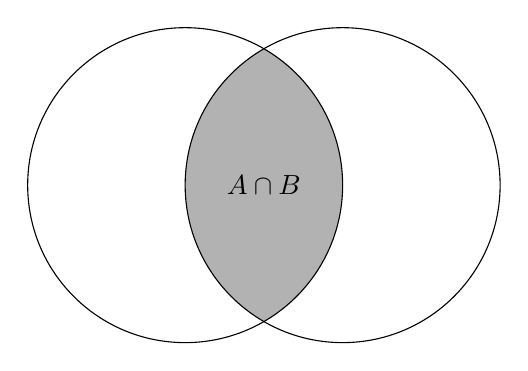
\begin{tikzpicture}
			\path[save path=\pathA](-1,0)circle(2cm);
			\path[save path=\pathB](1,0)circle(2cm);
			\begin{scope}
				\clip[use path=\pathA];
				\fill[black!30][use path=\pathB];
			\end{scope}
			\draw[use path=\pathA];
			\draw[use path=\pathB];
			\draw(0,0)node{\(A \cap B\)};
		\end{tikzpicture}
		\subcaption{集合的交}
	\end{subfigure}%
	\begin{subfigure}[b]{\subwidth}
		\centering
		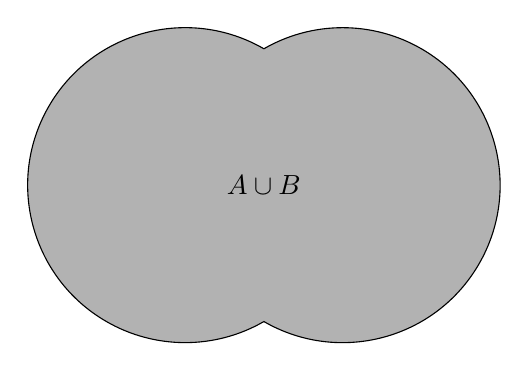
\begin{tikzpicture}
			\filldraw[fill=black!30,draw=black]
				(0,{sqrt(3)})arc[start angle=60,end angle=300,radius=2]
				arc[start angle=240,end angle=480,radius=2];
			\draw(0,0)node{\(A \cup B\)};
			\pgfresetboundingbox
			\path[use as bounding box] (-3,-2)rectangle(3,2);
		\end{tikzpicture}
		\subcaption{集合的并}
	\end{subfigure}%

	\begin{subfigure}[b]{\linewidth}
		\centering
		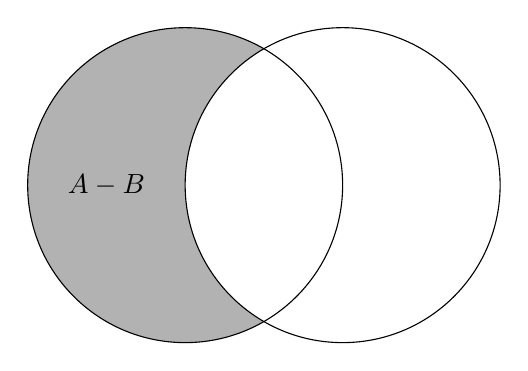
\begin{tikzpicture}
			\fill[black!30](0,{sqrt(3)})arc[start angle=60,end angle=300,radius=2]
				arc[start angle=240,end angle=120,radius=2];
			\draw(-1,0)circle(2cm);
			\draw(1,0)circle(2cm);
			\draw(-2,0)node{\(A-B\)};
			\pgfresetboundingbox
			\path[use as bounding box] (-3,-2)rectangle(3,2);
		\end{tikzpicture}
		\subcaption{集合的差}
	\end{subfigure}%
	\caption{韦恩图}
	\label{figure:集合论.韦恩图}
\end{figure}

\begin{property}
集合的运算满足以下性质:
\begin{enumerate}
\item 幂等律
\begin{gather}
	A \cap A = A, \\
	A \cup A = A.
\end{gather}

\item 交换律({\rm Commutative laws})
\begin{gather}
	A \cap B = B \cap A, \label{equation:集合论.集合代数公式1-1} \\
	A \cup B = B \cup A. \label{equation:集合论.集合代数公式1-2}
\end{gather}

\item 结合律({\rm Associative laws})
\begin{gather}
	(A \cap B) \cap C = A \cap (B \cap C), \label{equation:集合论.集合代数公式2-1} \\
	(A \cup B) \cup C = A \cup (B \cup C). \label{equation:集合论.集合代数公式2-2}
\end{gather}

\item 分配律({\rm Distributive laws})
\begin{gather}
	(A \cap B) \cup C = (A \cup C) \cap (B \cup C), \label{equation:集合论.集合代数公式3-1} \\
	(A \cup B) \cap C = (A \cap C) \cup (B \cap C), \label{equation:集合论.集合代数公式3-2} \\
	A \cup \bigcap \mathscr{B} = \bigcap\Set{A \cup X \given X \in \mathscr{B}}, \quad(\mathscr{B}\neq\emptyset) \label{equation:集合论.集合代数公式3-3} \\
	A \cap \bigcup \mathscr{B} = \bigcup\Set{A \cap X \given X \in \mathscr{B}}, \label{equation:集合论.集合代数公式3-4} \\
	\Powerset (A \cup B) \supseteq \Powerset A \cup \Powerset B, \label{equation:集合论.集合代数公式3-5} \\ %@see: 《Elements of Set Theory》 P26 Exercise 7(b).
	\Powerset (A \cap B) = \Powerset A \cap \Powerset B. \label{equation:集合论.集合代数公式3-6} %@see: 《Elements of Set Theory》 P26 Exercise 7(a)
\end{gather}

%@see: https://mathworld.wolfram.com/deMorgansLaws.html
\item 对偶律({\rm De Morgan's laws})(假设\(\mathscr{A}\neq\emptyset\))
\begin{gather}
	\Omega - (A \cap B)
	= (\Omega - A) \cup (\Omega - B), \label{equation:集合论.集合代数公式4-1} \\
	\Omega - (A \cup B)
	= (\Omega - A) \cap (\Omega - B), \label{equation:集合论.集合代数公式4-2} \\
	\Omega - \bigcup\mathscr{A}
	= \bigcap\Set{\Omega - X \given X\in\mathscr{A}}, \label{equation:集合论.集合代数公式4-3} \\
	\Omega - \bigcap\mathscr{A}
	= \bigcup\Set{\Omega - X \given X\in\mathscr{A}}. \label{equation:集合论.集合代数公式4-4}
\end{gather}

\item 与空集\(\emptyset\)和全集\(\Omega\)的运算(假设\(A \subseteq \Omega\))
\begin{gather}
	A \cup \emptyset = A, \label{equation:集合论.集合代数公式5-1} \\
	A \cap \emptyset = \emptyset, \label{equation:集合论.集合代数公式5-2} \\
	A \cup \Omega = \Omega, \label{equation:集合论.集合代数公式5-3} \\
	A \cap \Omega = A, \label{equation:集合论.集合代数公式5-4} \\
	A \cup (\Omega - A) = \Omega, \label{equation:集合论.集合代数公式5-5} \\
	A \cap (\Omega - A) = \emptyset, \label{equation:集合论.集合代数公式5-6} \\
	A \cup (A \cap B) = A, \\
	A \cap (A \cup B) = A, \\
	\Omega - \emptyset = \Omega, \\
	\Omega - \Omega = \emptyset, \\
	\Omega - (\Omega - A) = A.
\end{gather}

\item 包含关系
\begin{gather}
	A \subseteq B \implies A \cup C \subseteq B \cup C, \label{equation:集合论.集合代数公式6-1} \\
	A \subseteq B \implies A \cap C \subseteq B \cap C, \label{equation:集合论.集合代数公式6-2} \\
	A \subseteq B \implies \bigcup A \subseteq \bigcup B, \label{equation:集合论.集合代数公式6-3} \\
	A \subseteq B \implies (\Omega - B) \subseteq (\Omega - A), \label{equation:集合论.集合代数公式6-4} \\
	\emptyset \neq A \subseteq B \implies \bigcap B \subseteq \bigcap A, \label{equation:集合论.集合代数公式6-5} \\
	A \cap B \subseteq A, \\
	A \subseteq A \cup B.
\end{gather}

\item 差集
\begin{gather}
	A - B \subseteq A, \\
	B \subseteq \Omega
	\implies
	A - B = A \cap (\Omega - B), \\
	A \cup B = B
		\iff A \subseteq B
		\iff A \cap B = A
		\iff A - B = \emptyset, \label{equation:集合论.集合代数公式7-3} \\
	A \oplus B = B \oplus A, \\
	(A \oplus B) \oplus C = A \oplus (B \oplus C), \\
	A \oplus \emptyset = A, \\
	A \oplus A = \emptyset, \\
	A \oplus B = A \oplus C
		\iff B = C.
\end{gather}
\end{enumerate}
\begin{proof}
对\cref{equation:集合论.集合代数公式1-1} 证明如下:
\begin{align*}
	x \in A \cap B
	&\iff x \in A \land x \in B \\
	&\iff x \in B \land x \in A \\
	&\iff x \in B \cap A.
\end{align*}

对\cref{equation:集合论.集合代数公式1-2} 证明如下:
\begin{align*}
	x \in A \cup B
	&\iff x \in A \lor x \in B \\
	&\iff x \in B \lor x \in A \\
	&\iff x \in B \cup A.
\end{align*}

对\cref{equation:集合论.集合代数公式2-1} 证明如下:
\begin{align*}
	x \in (A \cap B) \cap C
	&\iff x \in A \cap B \land x \in C \\
	&\iff (x \in A \land x \in B) \land x \in C \\
	&\iff x \in A \land (x \in B \land x \in C) \\
	&\iff x \in A \land x \in B \cap C \\
	&\iff x \in A \cap (B \cap C).
\end{align*}

对\cref{equation:集合论.集合代数公式2-2} 证明如下:
\begin{align*}
	x \in (A \cup B) \cup C
	&\iff x \in A \cup B \lor x \in C \\
	&\iff (x \in A \lor x \in B) \lor x \in C \\
	&\iff x \in A \lor (x \in B \lor x \in C) \\
	&\iff x \in A \lor x \in B \cup C \\
	&\iff x \in A \cup (B \cup C).
\end{align*}

对\cref{equation:集合论.集合代数公式3-5} 证明如下:
\begin{align*}
	x \in \Powerset A \cup \Powerset B
	&\iff x \in \Powerset A \lor x \in \Powerset B \\
	&\iff x \subseteq A \lor x \subseteq B \\
	&\implies x \subseteq A \cup B \\
	&\iff x \in \Powerset (A \cup B),
\end{align*}
注意到中间步骤的\(\implies\)通常不是可逆的,
这是因为只要取\(a \subseteq A - B, b \subseteq B - A, x = a \cup b\),
就有\(x \subseteq A \cup B\)但是\(x \not\subseteq A \land x \not\subseteq B\),
因此\(x \subseteq A \cup B \notimplies x \subseteq A \lor x \subseteq B\).
%从上面的证明过程可以看出,
%要使\(\Powerset (A \cup B) = \Powerset A \cup \Powerset B\)成立,
%必有\[
%	\forall x \bigl(
%		x \subseteq A \cup B
%		\iff
%		x \subseteq A \lor x \subseteq B
%	\bigr)
%\]成立.
%取\(x = A \cup B\),
%由\(x \subseteq A \lor x \subseteq B\)
%可得\[
%	A \cup B = A \lor A \cup B = B.
%\]
%因此,当且仅当\(A \cup B \in \Set{A,B}\)时,
%就有\(\Powerset (A \cup B) = \Powerset A \cup \Powerset B\)成立.

对\cref{equation:集合论.集合代数公式3-6} 证明如下:
\begin{align*}
	x \in \Powerset (A \cap B)
	&\iff x \subseteq A \cap B \\
	&\iff x \subseteq A \land x \subseteq B \\
	&\iff x \in \Powerset A \land x \in \Powerset B \\
	&\iff x \in \Powerset A \cap \Powerset B.
\end{align*}

对\cref{equation:集合论.集合代数公式6-5} 证明如下:
\begin{align*}
	A \subseteq B
	&\iff (\forall t)[t \in A \implies t \in B] \\
	&\implies (\forall x)[
		(\forall b)[b \in B \implies x \in b]
		\implies
		(\forall a)[a \in A \implies x \in a]
	] \\
	&\iff (\forall x)[x \in \bigcap B \implies x \in \bigcap A].
	\qedhere
\end{align*}
\end{proof}
\end{property}

\begin{example}
%@see: 《Elements of Set Theory》 P32 Exercise 21.
设\(A,B\)是集合.
证明:\begin{equation}\label{equation:集合论.并集的并等于并的并集}
	\bigcup(A \cup B) = \bigcup A \cup \bigcup B.
\end{equation}
\begin{proof}
直接计算得
\begin{align*}
	x \in \bigcup(A \cup B)
	&\iff
	(\exists t)[t \in A \cup B \implies x \in t] \\
	&\iff
	(\exists t)[t \in A \lor t \in B \implies x \in t] \\
	&\iff
	(\exists t)[t \in A \implies x \in t] \lor (\exists t)[t \in B \implies x \in t] \\
	&\iff
	x \in \bigcup A \lor x \in \bigcup B \\
	&\iff
	x \in \bigcup A \cup \bigcup B.
	\qedhere
\end{align*}
\end{proof}
\end{example}

\begin{example}
%@see: 《Elements of Set Theory》 P32 Exercise 22.
设\(A,B\)是非空集合.
证明:\begin{equation}
	\bigcap(A \cup B) = \bigcap A \cap \bigcap B.
\end{equation}
%\begin{proof}
%直接计算得
%\begin{align*}
%	x \in \bigcap(A \cup B)
%	&\iff
%	x \in \bigcap A \land x \in \bigcap B \\
%	&\iff
%	x \in \bigcap A \cap \bigcap B.
%	\qedhere
%\end{align*}
%\end{proof}
\end{example}

\begin{example}
证明:\begin{equation}
	(A \cup B) - (A \cap B) = (A-B)\cup(B-A).
\end{equation}
\begin{proof}
根据集合交、并、差的定义,有
\begin{align*}
	x \in (A \cup B) - (A \cap B)
	&\iff x \in (A \cup B) \land x \notin (A \cap B) \\
	&\iff (x \in A \lor x \in B) \land \neg(x \in A \land x \in B) \\
	&\iff (x \in A \land \neg(x \in A \land x \in B))
	 \lor (x \in B \land \neg(x \in A \land x \in B)) \\
	&\iff (x \in A \land (x \notin A \lor x \notin B))
	 \lor (x \in B \land (x \notin A \lor x \notin B)) \\
	&\iff (x \in A \land x \notin B) \lor (x \in B \land x \notin A) \\
	&\iff x \in (A-B)\cup(B-A).
\qedhere
\end{align*}
\end{proof}
\end{example}

\input{集合论/集合论/关系}
\section{映射}
\subsection{映射的概念}
\begin{definition}
%@see: 《Elements of Set Theory》 P42 Definition
设\(F\)是关系,如果\[
	(\forall x \in \dom F)(\exists! y)[\opair{x,y} \in F],
\]
则称“关系\(F\)是一个\DefineConcept{映射}(function)”.
\end{definition}
可以从映射的定义中看出,虽然映射也是关系,
但映射有一般的关系所没有的特殊性质:
映射是\DefineConcept{单值的}(single-valued).
换句话说,对于关系\(F\),每个\(x\)可能对应若干个\(y\);
但是,对于映射\(F\),每个\(x\)就只对应一个\(y\).
我们可以把\(x\)与\(y\)这两个元素之间的对应关系记为\(x \mapsto y\).

我们把使得\(xFy\)成立的\(y\)称为“\(x\)(在映射\(F\)下)的\DefineConcept{像}%
(the \emph{value} of \(F\) at \(x\))”,
记为\(F(x)\),即\[
	y = f(x);
\]
称\(x\)为“\(y\)(在映射\(F\)下)的一个\DefineConcept{原像}”.
这里用的\(F(x)\)符号是欧拉提出的,
我们仅当\(F\)是一个映射且\(x\in\dom F\)时使用这个记号.
不过,我们也可以定义:\[
	F(x) \defeq \bigcup\Set{ y \given \opair{x,y} \in F }.
\]
它对于任意\(F\)和\(x\)都有意义.

映射是如此重要,以至于各家对用于描述映射的术语没有达成统一.
以下是两种最常采用的术语.

设\(X,Y\)都是集合,
如果\(f\)是一个映射,且\(\dom f = X\),\(\ran f \subseteq Y\),
则称“\(f\)是从\(X\)到\(Y\)的\DefineConcept{映射}%
(\(f\) is a function \emph{from} \(X\) \emph{into} \(Y\))”,
或称“\(f\)将\(X\)映射到\(Y\)里%
(\(f\) \emph{maps} \(X\) \emph{into} \(Y\))”,
记作\[
	f\colon X \to Y.
\]
如果还有\(\ran f = Y\),
那么称“\(f\)是从\(X\)到\(Y\)上的映射%
(\(f\) is a function from \(X\) \emph{onto} \(Y\))”,
或称“\(f\)将\(X\)映射到\(Y\)上%
(\(f\) \emph{maps} \(X\) \emph{onto} \(Y\))”,
或称“\(f\)是\DefineConcept{满射}(surjective)”.
我们可以说“任意映射总将它的定义域映射到它的值域上”,
还可以说“任意映射总把它的定义域映射到以它的值域为子集的任意集合\(B\)里”.
注意到两种说法的区别,“上”字和“里”字的选用,
不光取决于映射\(f\)本身,还取决于我们讨论的集合\(B\).

如果\[
	(\forall y \in \ran f)
	(\exists! x)
	[\opair{x,y} \in f],
\]
那么称“映射\(f\)是\DefineConcept{一对一的}(one-to-one)”.

有时候我们希望把“一对一的”这个概念套用到一般的关系上,
它们往往不是映射,因此我们类比于“单值的”,创造出“单根的”这个概念.
\begin{definition}
%@see: 《Elements of Set Theory》 P43 Definition
如果集合\(R\)满足\[
	(\forall y \in \ran R)
	(\exists! x)
	[\opair{x,y} \in R],
\]
则称“\(R\)是\DefineConcept{单根的}(single-rooted)”.
\end{definition}

因此,我们可以说,“一个映射是单根的”当且仅当“这个映射是一对一的”.

如果\[
	(\forall x_1, x_2 \in \dom f)
	[x_1 \neq x_2 \implies f(x_1) \neq f(x_2)],
\]
那么称“\(f\)是\DefineConcept{单射}(injective)”.

由于映射本就是单值的,若它还是单根的,那么这个映射就是单射.
换句话说,“一对一的映射”和“单射”是相同的概念.

如果\(f\)既是单射,又是满射,
那么称“\(f\)是\DefineConcept{双射}(bijective)
或\DefineConcept{一一映射}”.

我们可以给出一个最平凡的一一映射.
\begin{definition}
设\(X\)是集合.
我们把\[
	\Set{ \opair{x,x} \given x \in X }
\]称为“(\(X\)上的)\DefineConcept{恒等映射}或\DefineConcept{恒同映射}”,
常记为\(i_X\).
\end{definition}

\begin{example}
%@see: 《Elements of Set Theory》 P52 Exercise 11
设\(F,G\)都是映射,
\(\dom F = \dom G = X\),且\[
	(\forall x \in X)[F(x) = G(x)].
\]
证明:\(F=G\).
\begin{proof}
显然有
\begin{align*}
	F=G
	&\iff (\forall x \in X)(\exists!y)[
		\opair{x,y} \in F
		\iff
		\opair{x,y} \in G
	] \\
	&\iff (\forall x \in X)(\exists!y)[
		y = F(x) = G(x)
	] \\
	&\iff (\forall x \in X)[F(x) = G(x)].
	\qedhere
\end{align*}
\end{proof}
\end{example}

\begin{example}
%@see: 《Elements of Set Theory》 P52 Exercise 12
设\(f,g\)都是映射.
证明:\[
	f \subseteq g
	\iff
	\dom f \subseteq \dom g
	\land
	(\forall x \in \dom f)
	[f(x) = g(x)].
\]
\begin{proof}
直接有
\begin{align*}
	f \subseteq g
	&\iff (\forall x)(\exists!y)[\opair{x,y} \in f \implies \opair{x,y} \in g] \\
	&\iff (\forall x \in \dom f)[x \in \dom g]\land(\forall x \in \dom f)(\exists!y)[y=f(x)=g(x)] \\
	&\iff [\dom f \subseteq \dom g]\land(\forall x \in \dom f)[f(x)=g(x)].
	\qedhere
\end{align*}
\end{proof}
\end{example}

\begin{example}
%@see: 《Elements of Set Theory》 P53 Exercise 13
设\(f,g\)都是映射,\(f \subseteq g\)且\(\dom g \subseteq \dom f\).
证明:\(f=g\).
%TODO
\end{example}

\begin{example}
%@see: 《Elements of Set Theory》 P53 Exercise 14
设\(f,g\)都是映射.
证明:
\begin{enumerate}
	\item \(f \cap g\)是映射.
	\item \(f \cup g\)是映射的充分必要条件是\[
		(\forall x \in (\dom f)\cap(\dom g))[f(x)=g(x)].
	\]
\end{enumerate}
%TODO
\end{example}

\begin{example}
%@see: 《Elements of Set Theory》 P53 Exercise 15
\def\A{\mathscr{A}}%
设\(\A\)是一组映射,且\[
	(\forall f,g\in\A)[f \subseteq g \lor g \subseteq f].
\]
证明:\(\bigcup\A\)也是映射.
%TODO
\end{example}

\begin{example}
%@see: 《Elements of Set Theory》 P53 Exercise 16
证明:不存在一个集合,使得每个映射都属于它.
%TODO
\end{example}

\begin{example}
%@see: 《实变函数论》(周民强) P14 思考题5.
设\(f\colon X \to Y,
g\colon Y \to X\).
证明:若\[
	(\forall x \in X)[g(f(x)) = x],
\]
则\(f\)是单射,\(g\)是满射.
%TODO
\end{example}

\subsection{逆,复合,限制,像,原像}
以下定义的操作通常用在映射上,有时候也用于关系,但也可以用于任意集合.
\begin{definition}
设\(A,F,G\)都是集合.
\begin{enumerate}
	\item 称集合\[
		\Set*{ \opair{u,v} \given \opair{v,u} \in F }
	\]为“\(F\)的\DefineConcept{逆}%
	(the \emph{inverse} of \(F\))”,
	记作\(F^{-1}\).

	特别地,如果\(F^{-1}\)是映射,
	则称“\(F^{-1}\)是\(F\)的\DefineConcept{逆映射}”.

	\item 称集合\[
		\Set*{ \opair{u,v} \given (\exists t)[\opair{u,t} \in G \land \opair{t,v} \in F] }
	\]为“\(F\)和\(G\)的\DefineConcept{复合}%
	(the \emph{composition} of \(F\) and \(G\))”,
	记作\(F \circ G\).

	\item 称集合\[
		\Set*{ \opair{u,v} \given \opair{u,v} \in F \land u \in A }
	\]为“\(F\)在\(A\)上的\DefineConcept{限制}%
	(the \emph{restriction} of \(F\) to \(A\))”,
	记作\(F \upharpoonright A\).

	\item 称集合\[
		\Set*{ v \given (\exists u \in A)[\opair{u,v} \in F] }
	\]为“\(A\)在\(F\)下的\DefineConcept{像}%
	(the \emph{image} of \(A\) \emph{under} \(F\))”,
	记作\(F\ImageOfSetUnderRelation{A}\).
\end{enumerate}
\end{definition}

当\(F\)是一个映射,且\(A \subseteq \dom F\)时,
\(F\ImageOfSetUnderRelation{A}\)这个概念可能更容易理解,
因为这时候\[
	F\ImageOfSetUnderRelation{A}
	= \Set{ F(u) \given u \in A }.
\]

我们可以利用子集公理构造出上述定义下的所需集合的存在性.
特别地,\[
	F^{-1} \subseteq \ran F \times \dom F, \qquad
	F \circ G \subseteq \dom G \times \ran F,
\]\[
	F \upharpoonright A \subseteq F, \qquad
	F\ImageOfSetUnderRelation{A} \subseteq \ran F.
\]

例如,我们可以按如下方法正当化“关系\(F\)的逆”的定义:
根据子集公理,存在集合\(B\),使得对于任意\(x\),总有\begin{align*}
	x \in B
	&\iff
	[x \in \ran F \times \dom F]
	\land
	(\exists u)(\exists v)[x = \opair{u,v} \land \opair{v,u} \in F], \\
	&\iff
	(\exists u)(\exists v)[x = \opair{u,v} \land \opair{v,u} \in F].
\end{align*}
再根据外延公理,可以保证集合\(B\)的唯一性.
因此我们可以将集合\(B\)记为\(F^{-1}\).

\begin{definition}
%@see: 《点集拓扑讲义(第四版)》(熊金城) P22 定义1.5.4
设\(A,B,X\)都是集合,\(A \subset B\).
若映射\(F\colon A \to X\)和\(G\colon B \to X\)满足\(F \subset G\),
则称“\(G\)是\(F\)在\(B\)上的\DefineConcept{扩张}”.
\end{definition}

\begin{theorem}
\(F \upharpoonright \emptyset = \emptyset\).
\end{theorem}

\begin{theorem}
\(F\ImageOfSetUnderRelation{A} = \ran(F \upharpoonright A)\).
\begin{proof}
根据值域的定义有\begin{align*}
	v \in \ran(F \upharpoonright A)
	&\iff
	(\exists u)[\opair{u,v} \in F \upharpoonright A] \\
	&\iff
	(\exists u)[\opair{u,v} \in F \land u \in A] \\
	&\iff
	v \in F\ImageOfSetUnderRelation{A}.
	\qedhere
\end{align*}
\end{proof}
\end{theorem}

\begin{definition}
设\(F\)是关系,\(A\)是集合,那么称集合\[
	\Set*{ x \in \dom F \given F(x) \in A }
\]为“集合\(A\)在关系\(F\)下的\DefineConcept{原像}%
(the \emph{inverse image} of \(A\) under \(F\))”,
记作\(F^{-1}\ImageOfSetUnderRelation{A}\).
\end{definition}

一般来说,一个映射的逆不一定是映射.
例如,\(F=\Set{ \opair{1,1},\opair{2,1} }\)是一个映射,
但它的逆\(F^{-1}=\Set{ \opair{1,1},\opair{1,2} }\)不是映射.

\begin{theorem}\label{theorem:集合论.关系的逆的定义域值域以及关系的二重逆}
%@see: 《Elements of Set Theory》 P46 Theorem 3E
设\(F\)是集合,则有\begin{gather}
	\dom F^{-1} = \ran F, \\
	\ran F^{-1} = \dom F.
\end{gather}

如果\(F\)是关系,则有\begin{equation}
	(F^{-1})^{-1} = F.
\end{equation}
\begin{proof}
因为\[
	y \in \dom F^{-1}
	\iff
	(\exists x)[yF^{-1}x]
	\iff
	(\exists x)[xFy]
	\iff
	y \in \ran F,
\]
所以\(\dom F^{-1} = \ran F\).

因为\[
	x \in \ran F^{-1}
	\iff
	(\exists y)[yF^{-1}x]
	\iff
	(\exists y)[xFy]
	\iff
	x \in \dom F,
\]
所以\(\ran F^{-1} = \dom F\).

因为\[
	\opair{x,y} \in (F^{-1})^{-1}
	\iff
	\opair{y,x} \in F^{-1}
	\iff
	\opair{x,y} \in F,
\]
所以\((F^{-1})^{-1} = F\).
\end{proof}
\end{theorem}

\begin{theorem}\label{theorem:集合论.关系及其逆是映射的充分必要条件}
%@see: 《Elements of Set Theory》 P46 Theorem 3F
设\(F\)是集合,则“\(F^{-1}\)是映射”的充分必要条件是:\(F\)是单根的.

设\(F\)是关系,则“\(F\)是映射”的充分必要条件是:\(F^{-1}\)是单根的.
\begin{proof}
容易看出\begin{align*}
	\text{\(F^{-1}\)是映射}
	&\iff
	\text{\(F^{-1}\)是单值的} \\
	&\iff
	(\forall x \in \dom F^{-1})(\exists! y)[xF^{-1}y] \\
	&\iff
	(\forall x \in \ran F)(\exists! y)[yFx] \\
	&\iff
	\text{\(F\)是单根的}, \\
	\text{\(F\)是映射}
	&\iff
	\text{\(F\)是单值的} \\
	&\iff
	(\forall x \in \dom F)(\exists! y)[xFy] \\
	&\iff
	(\forall x \in \ran F^{-1})(\exists! y)[yF^{-1}x] \\
	&\iff
	\text{\(F^{-1}\)是单根的}.
	\qedhere
\end{align*}
\end{proof}
\end{theorem}

\begin{theorem}\label{theorem:集合论.逆映射的计算}
%@see: 《Elements of Set Theory》 P46 Theorem 3G
设\(F\)是单射.
\begin{enumerate}
	\item 如果\(x \in \dom F\),那么\[
		F^{-1}(F(x)) = x.
	\]

	\item 如果\(y \in \ran F\),那么\[
		F(F^{-1}(y)) = y.
	\]
\end{enumerate}
\begin{proof}
假设\(x \in \dom F\),
那么\(\opair{x,F(x)} \in F\),且\(\opair{F(x),x} \in F^{-1}\),
于是\(F(x) \in \dom F^{-1}\).
因为\(F\)是单射,是单根的,
所以由\cref{theorem:集合论.关系及其逆是映射的充分必要条件}
可知\(F^{-1}\)是映射,
从而\(x = F^{-1}(F(x))\).

如果\(y \in \ran F\),
那么根据本定理第1条,以及\((F^{-1})^{-1} = F\),可知\[
	F(F^{-1}(y)) = (F^{-1})^{-1}(F^{-1}(y)) = y.
	\qedhere
\]
\end{proof}
\end{theorem}

\begin{theorem}\label{theorem:集合论.映射的复合也是映射}
%@see: 《Elements of Set Theory》 P47 Theorem 3H
设\(F,G\)都是映射,则\(F \circ G\)是映射,且\[
	\dom(F \circ G)
	= \Set*{ x \in \dom G \given G(x) \in \dom F },
\]\[
	(\forall x \in \dom(F \circ G))
	[(F \circ G)(x) = F(G(x))].
\]
\begin{proof}
要证\(F \circ G\)是一个映射,
假设有\(\opair{x,y} \in F \circ G\)和\(\opair{x,z} \in F \circ G\)同时成立.
那么,\[
	(\exists p)[\opair{x,p} \in G \land \opair{p,y} \in F]
	\quad\text{和}\quad
	(\exists q)[\opair{x,q} \in G \land \opair{q,z} \in F]
\]同时成立.
既然\(G\)是映射,必有\(p = q\).
同理,\(F\)是映射,必有\(y = z\).
因此\(F \circ G\)是映射.

现在再假设\(x \in \dom G\)且\(G(x) \in \dom F\).
我们必须证明\[
	x \in \dom(F \circ G)
	\quad\text{和}\quad
	(F \circ G)(x) = F(G(x)).
\]
我们知道\[
	\opair{x,G(x)} \in G,
	\qquad
	\opair{G(x),F(G(x))} \in F.
\]
因此\(\opair{x,F(G(x))} \in F \circ G\).

反过来说,如果\(x \in \dom(F \circ G)\),
那么就有\[
	(\exists y)(\exists t)
	[\opair{x,t} \in G \land \opair{t,y} \in F].
\]
于是就有\(x \in \dom G\)和\(t = G(x) \in \dom F\).
\end{proof}
\end{theorem}

容易看出,映射的复合是有顺序的,
\(f \circ g\)有意义并不代表\(g \circ f\)也有意义.
即便两者都有意义,它们也未必相同.

\begin{example}
%@see: 《Elements of Set Theory》 P47 Example
假设\(G\)是单射,
那么,根据\cref{theorem:集合论.映射的复合也是映射},
\(G^{-1} \circ G\)也是一个映射,
它的定义域为\[
	\Set{ x \in \dom G \given G(x) \in \dom G^{-1} }
	= \dom G,
\]
并且,对于\(\forall x \in \dom(G^{-1} \circ G)\),
有\begin{align*}
	(G^{-1} \circ G)(x) &= G^{-1}(G(x)) \\
	&= x. \tag{\cref{theorem:集合论.逆映射的计算}}
\end{align*}
因此,\(G^{-1} \circ G\)就是\(I_{\dom G}\),
\(\dom G\)上的恒等映射.
同理,\(G \circ G^{-1}\)是\(I_{\ran G}\),
\(\ran G\)上的恒等映射.
\end{example}

\begin{theorem}
%@see: 《Elements of Set Theory》 P65 Exercise 53.
设\(R,S\)是集合,那么\begin{gather}
	(R \cup S)^{-1} = R^{-1} \cup S^{-1},
	\label{equation:集合论.并的逆等于逆的并} \\
	(R \cap S)^{-1} = R^{-1} \cap S^{-1},
	\label{equation:集合论.交的逆等于逆的交} \\
	(R - S)^{-1} = R^{-1} - S^{-1}.
	\label{equation:集合论.差的逆等于逆的差}
\end{gather}
\begin{proof}
对\cref{equation:集合论.并的逆等于逆的并} 证明如下:
\begin{align*}
	\opair{x,y} \in (R \cup S)^{-1}
	&\iff \opair{y,x} \in R \cup S \\
	&\iff \opair{y,x} \in R \lor \opair{y,x} \in S \\
	&\iff \opair{x,y} \in R^{-1} \lor \opair{x,y} \in S^{-1} \\
	&\iff \opair{x,y} \in R^{-1} \cup S^{-1}.
\end{align*}

对\cref{equation:集合论.交的逆等于逆的交} 证明如下:
\begin{align*}
	\opair{x,y} \in (R \cap S)^{-1}
	&\iff \opair{y,x} \in R \cap S \\
	&\iff \opair{y,x} \in R \land \opair{y,x} \in S \\
	&\iff \opair{x,y} \in R^{-1} \land \opair{x,y} \in S^{-1} \\
	&\iff \opair{x,y} \in R^{-1} \cap S^{-1}.
\end{align*}

对\cref{equation:集合论.差的逆等于逆的差} 证明如下:
\begin{align*}
	\opair{x,y} \in (R - S)^{-1}
	&\iff \opair{y,x} \in R - S \\
	&\iff \opair{y,x} \in R \land \opair{y,x} \notin S \\
	&\iff \opair{x,y} \in R^{-1} \land \opair{x,y} \notin S^{-1} \\
	&\iff \opair{x,y} \in R^{-1} - S^{-1}.
	\qedhere
\end{align*}
\end{proof}
\end{theorem}

\begin{theorem}\label{theorem:集合论.复合的逆}
%@see: 《Elements of Set Theory》 P47 Theorem 3I
设\(F,G\)都是集合,那么\[
	(F \circ G)^{-1} = G^{-1} \circ F^{-1}.
\]
\begin{proof}
易知\((F \circ G)^{-1}\)和\(G^{-1} \circ F^{-1}\)都是关系,且\begin{align*}
	\opair{x,y} \in (F \circ G)^{-1}
	&\iff
	\opair{y,x} \in F \circ G \\
	&\iff
	(\exists t)[\opair{y,t} \in G \land \opair{t,x} \in F] \\
	&\iff
	(\exists t)[\opair{x,t} \in F^{-1} \land \opair{t,y} \in G^{-1}] \\
	&\iff
	\opair{x,y} \in G^{-1} \circ F^{-1}.
	\qedhere
\end{align*}
\end{proof}
\end{theorem}

由\cref{theorem:集合论.复合的逆} 立即可得如下推论.
\begin{proposition}\label{theorem:集合论.复合的逆.推论1}
设\(F\)是集合,那么\[
	(F^{-1} \circ F)^{-1} = F^{-1} \circ F.
\]
\end{proposition}

\begin{axiom}[选择公理(第一种形式)]
对于任意关系\(R\),存在映射\(H\),满足\[
	H \subseteq R,
	\quad\text{且}\quad
	\dom H = \dom R.
\]
\end{axiom}

\begin{theorem}
%@see: 《Elements of Set Theory》 P48 Theorem 3J
设映射\(F\colon A \to B\),其中\(A\)是非空集合.
\begin{enumerate}
	\item “存在映射\(G\colon B \to A\)(称其为\DefineConcept{左逆}),
	使得\(G \circ F\)是\(A\)上的恒等映射\(I_A\)”是“\(F\)是单射”的充分必要条件.

	\item “存在映射\(H\colon B \to A\)(称其为\DefineConcept{右逆}),
	使得\(F \circ H\)是\(B\)上的恒等映射\(I_B\)”是“\(F\)是满射”的充分必要条件.
\end{enumerate}
\begin{proof}
\begin{enumerate}
	\item
	先证充分性.
	我们假设存在映射\(G\)使得\(G \circ F = I_A\).
	如果\(F(x) = F(y)\),那么\[
		x = G(F(x)) = G(F(y)) = y,
	\]
	于是\(F\)是单射.

	再证必要性.
	假设\(F\)是单射,
	那么根据\cref{theorem:集合论.关系的逆的定义域值域以及关系的二重逆,theorem:集合论.关系及其逆是映射的充分必要条件},
	\(F^{-1}\)是一个从\(\ran F\)到\(A\)上的映射.
	现在我们需要将\(F^{-1}\)延拓为以\(B\)为定义域的映射\(G\).
	因为\(A\)是非空集合,
	于是我们可以取定\(a \in A\),
	然后令\[
		G(x) = \left\{ \begin{array}{ll}
			F^{-1}(x), & x \in \ran F, \\
			a, & x \in B - \ran F,
		\end{array} \right.
	\]或者令\[
		G = F^{-1} \cup (B - \ran F) \times \Set{a}.
	\]
	这个构造出来的映射\(G\)是一个从\(B\)到\(A\)里的映射,
	且满足\[
		\dom(G \circ F) = A,
	\]
	以及\[
		(\forall x \in A)[G(F(x)) = F^{-1}(F(x)) = x],
	\]
	于是\(G \circ F = I_A\)成立.

	\item
	我们还是先证充分性.
	假设存在映射\(H\)使得\(F \circ H = I_B\).
	那么\[
		(\forall y \in B)[y = F(H(y))],
	\]
	从而\(y \in \ran F\),
	于是\(\ran F = B\).

	必要性的证明稍显困难.
	我们不能直接取\(H = F^{-1}\),
	因为一般而言\(F\)不会是单射,
	\(F^{-1}\)也不会是一个映射.
	假设\(F\)将\(A\)映射到\(B\)上,\(\ran F = B\).
	现在我们需要为每个\(y \in B\)选择某个\(x\),使得\(F(x) = y\),然后令\(H(y) = x\);
	考虑到\(y \in \ran F\),这样的\(x\)必定存在.
	虽然我们知道对于每个\(y\),存在一个合适的\(x\),
	但是我们无法据此构造所求映射\(H\).
	因此,我们需要引入选择公理.
	借助选择公理,我们可以令映射\(H\)满足\(H \subseteq F^{-1}\)且\(\dom H = \dom F^{-1} = B\).
	于是\(H\)满足\[
		(\forall y \in B)
		[
			\opair{y,H(y)} \in F^{-1}
			\iff
			\opair{H(y),y} \in F
			\iff
			F(H(y)) = y
		].
		\qedhere
	\]
\end{enumerate}
\end{proof}
\end{theorem}

\begin{theorem}
%@see: 《Elements of Set Theory》 P48 Theorem 3K
设\(A,B,F\)都是集合.
\def\F#1{F\ImageOfSetUnderRelation{#1}}
\begin{enumerate}
	\item 并的像是像的并:\begin{gather}
		\F{A \cup B}
		= \F{A} \cup \F{B},
		\label{equation:集合论.并的像与像的并的关系1} \\
		\F{\bigcup A}
		= \bigcup\Set{ \F{a} \given a \in A }.
		\label{equation:集合论.并的像与像的并的关系2}
	\end{gather}

	\item 交的像包含于像的交:\begin{gather}
		\F{A \cap B}
		\subseteq \F{A} \cap \F{B},
		\label{equation:集合论.交的像与像的交的关系1} \\
		\F{\bigcap A}
		\subseteq \bigcap\Set{ \F{a} \given a \in A }.
		\label{equation:集合论.交的像与像的交的关系2}
		\quad(A \neq \emptyset)
	\end{gather}
	若\(F\)是单根的,则以上两式取“=”号.

	\item 差的像包含像的差:\begin{equation}
		\F{A} - \F{B}
		\subseteq \F{A-B}.
		\label{equation:集合论.差的像与像的差的关系}
	\end{equation}
	若\(F\)是单根的,则上式取“=”号.
\end{enumerate}
\begin{proof}
\cref{equation:集合论.并的像与像的并的关系1} 证明如下:
\begin{align*}
	y \in \F{A \cup B}
	&\iff (\exists x \in A \cup B)[\opair{x,y} \in F] \\
	&\iff (\exists x \in A)[\opair{x,y} \in F]
			\lor (\exists x \in B)[\opair{x,y} \in F] \\
	&\iff y \in \F{A} \lor y \in \F{B}.
\end{align*}

\cref{equation:集合论.交的像与像的交的关系1} 证明如下:
\begin{align*}
	y \in \F{A \cap B}
	&\iff (\exists x \in A \cap B)[\opair{x,y} \in F] \\
	&\implies (\exists x \in A)[\opair{x,y} \in F]
		\land (\exists x \in B)[\opair{x,y} \in F] \\
	&\iff y \in \F{A} \land y \in \F{B}.
\end{align*}
注意到中间步骤的\(\implies\)不总是可逆的,
这时因为虽然有\[
	(\exists x_1 \in A)[\opair{x_1,y} \in F], \qquad
	(\exists x_2 \in B)[\opair{x_2,y} \in F],
\]
但是可能\[
	(\forall x \in A \cap B)[\opair{x,y} \notin F].
\]
不过,如果\(F\)是单根的,那么必有\(x_1 = x_2 \in A \cap B\),
这时候中间步骤的\(\implies\)是可逆的,可以改为\(\iff\).

\cref{equation:集合论.并的像与像的并的关系2,equation:集合论.交的像与像的交的关系2} 分别是%
\cref{equation:集合论.并的像与像的并的关系1,equation:集合论.交的像与像的交的关系1} 的简单推广,
故略去证明.

\cref{equation:集合论.差的像与像的差的关系} 证明如下:
\begin{align*}
	y \in \F{A} - \F{B}
	&\iff (\exists x \in A)[\opair{x,y} \in F]
		\land \neg[(\exists t \in B)[\opair{t,y} \in F]] \\
	&\implies (\exists x \in A - B)[\opair{x,y} \in F] \\
	&\iff y \in \F{A - B}.
\end{align*}
若\(F\)是单根的,则\[
	(\exists! x)[\opair{x,y} \in F].
\]
这种情况下,中间步骤的\(\implies\)可以改为\(\iff\).
\end{proof}
\end{theorem}

\begin{corollary}
%@see: 《Elements of Set Theory》 P48 Corollary 3L
设\(G\)是映射,\(A,B\)都是集合.
\def\G#1{G^{-1}\ImageOfSetUnderRelation{#1}}
\begin{gather}
	\G{\bigcup A} = \bigcup\Set*{ \G{a} \given a \in A },
	\label{equation:集合论.并的原像与原像的并的关系} \\
	\G{\bigcap A} = \bigcap\Set*{ \G{a} \given a \in A }, \quad A \neq \emptyset,
	\label{equation:集合论.交的原像与原像的交的关系} \\
	\G{A - B} = \G{A} - \G{B}.
	\label{equation:集合论.差的原像与原像的差的关系}
\end{gather}
\end{corollary}

\begin{example}
%@see: 《Elements of Set Theory》 P53 Exercise 22.(a)
\def\F#1{F\ImageOfSetUnderRelation{#1}}
证明:\begin{equation}
	A \subseteq B \implies \F{A} \subseteq \F{B}.
\end{equation}
\begin{proof}
因为\(A \subseteq B\),所以\(A \cap B = A\),
那么由\cref{equation:集合论.交的像与像的交的关系1} 可知,\[
	\F{A} = \F{A \cap B} \subseteq \F{A} \cap \F{B} \subseteq \F{B}.
	\qedhere
\]
\end{proof}
\end{example}

\begin{example}
%@see: 《Elements of Set Theory》 P53 Exercise 22.(b)
证明:\begin{equation}
	(F \circ G)\ImageOfSetUnderRelation{A}
	= F\ImageOfSetUnderRelation{G\ImageOfSetUnderRelation{A}}.
\end{equation}
%TODO
\end{example}

\begin{example}
%@see: 《Elements of Set Theory》 P53 Exercise 22.(c)
证明:\begin{equation}
	Q \upharpoonright (A \cup B)
	= (Q \upharpoonright A)\cup(Q \upharpoonright B).
\end{equation}
%TODO
\end{example}

\begin{example}
%@see: 《Elements of Set Theory》 P65 Exercise 59.
设\(A,B,Q\)是集合.
证明:\begin{gather}
	Q \upharpoonright (A \cap B)
	= (Q \upharpoonright A) \cap (Q \upharpoonright B), \\
	Q \upharpoonright (A - B)
	= (Q \upharpoonright A)
	- (Q \upharpoonright B).
\end{gather}
%TODO
\end{example}

\begin{example}
%@see: 《Elements of Set Theory》 P65 Exercise 60.
设\(A,R,S\)是集合.
证明:\begin{equation}
	(R \circ S) \upharpoonright A = R \circ (S \upharpoonright A).
\end{equation}
%TODO
\end{example}

\begin{proposition}\label{theorem:集合论.与逆相等的充分必要条件}
设\(R\)是集合,
则\(R^{-1} \subseteq R
\iff R^{-1} = R
\iff R \subseteq R^{-1}\).
\begin{proof}
容易看出\begin{align*}
	R^{-1} \subseteq R
	&\iff
	(\forall x)(\forall y)[xR^{-1}y \implies xRy] \\
	&\iff
	(\forall x)(\forall y)[yRx \implies xRy] \\
	&\iff
	(\forall u)(\forall v)[uRv \implies vRu] \\
	&\iff
	(\forall u)(\forall v)[uRv \implies uR^{-1}v] \\
	&\iff
	R \subseteq R^{-1},
\end{align*}
再由\(R^{-1} \subseteq R \land R \subseteq R^{-1}\)
便得\(R = R^{-1}\).
\end{proof}
\end{proposition}

\subsection{有标集族,指标集}\label{section:集合论.指标集}
%@see: https://math.libretexts.org/Bookshelves/Mathematical_Logic_and_Proof/Book%3A_Mathematical_Reasoning__Writing_and_Proof_(Sundstrom)/05%3A_Set_Theory/5.05%3A_Indexed_Families_of_Sets
\begin{definition}
%@see: 《Elements of Set Theory》 P51
设\(F\)是映射,\(I\)是集合,\(\dom F \supseteq I\).

对于\(\forall i \in I\),
把\(i\)在映射\(F\)下的像\(F(i)\)记作\(F_i\),
即\[
	F_i \defeq F(i).
\]

把\(F\)在\(I\)上的限制\(F \upharpoonright I\)
称为“一个以\(I\)为指标集的\DefineConcept{有标集族}(an \emph{indexed family of sets} indexed by \(I\))”,
记作\(\{F_i\}_{i \in I}\),
即\[
	\{F_i\}_{i\in I}
	\defeq
	F \upharpoonright I.
\]
把\(I\)的每一个元素称为一个\DefineConcept{指标}(index).
把\(I\)称为“\(\{F_i\}_{i \in I}\)的\DefineConcept{指标集}(indexing set)”.
\end{definition}

\begin{example}
当我们谈到有标集族\(\{R\}_{i \in I}\)时,
我们指的就是映射\(F = I \times \{R\}\),
即对于每一个\(i \in I\)都指定同一个集合\(F(i) = R\).
\end{example}

\begin{example}
设\(\mathscr{A}\)是一个集族,
那么恒同映射\(\{A\}_{A \in \mathscr{A}} = \Set{ \opair{A,A} \given A \in \mathscr{A} }\)
就是一个以\(\mathscr{A}\)为指标集的有标集族.
有时候我们会把\(\{A\}_{A \in \mathscr{A}}\)简记为“有标集族\(\mathscr{A}\)”.
\end{example}

\begin{definition}
%@see: 《Elements of Set Theory》 P51
%@see: 《点集拓扑讲义(第四版)》(熊金城) P26 定义1.6.1
设有标集族\(\{F_i\}_{i \in I}\).

定义:\begin{equation}
	\bigcup_{i \in I} F_i
	\defeq
	\bigcup\Set{ F_i \given i \in I },
\end{equation}
把它称为“有标集族\(\{F_i\}_{i \in I}\)的并”.

当指标集\(I\)非空时,定义:
\begin{equation}
	\bigcap_{i \in I} F_i
	\defeq
	\bigcap\Set{ F_i \given i \in I },
\end{equation}
把它称为“有标集族\(\{F_i\}_{i \in I}\)的交”.
\end{definition}
应该注意到:
\(\bigcup_{i \in \emptyset} F_i = \emptyset\),
而\(\bigcap_{i \in \emptyset} F_i\)没有定义.

\begin{theorem}
%@see: 《点集拓扑讲义(第四版)》(熊金城) P26 定理1.6.1
设\(\{A_i\}_{i \in I}\)和\(\{B_j\}_{j \in J}\)是两个非空有标集族.
如果\[
	\Set{ A_i \given i \in I }
	= \Set{ B_j \given j \in J },
\]
则有\begin{gather}
	\bigcup_{i \in I} A_i = \bigcup_{j \in J} B_j, \\
	\bigcap_{i \in I} A_i = \bigcap_{j \in J} B_j.
\end{gather}
%TODO
\end{theorem}

\begin{theorem}
%@see: 《点集拓扑讲义(第四版)》(熊金城) P27 定理1.6.2
设\(\{A_i\}_{i \in I}\)是一个非空有标集族,
\(B\)是一个集合,
则\begin{itemize}
	\item 对于任意\(i_0 \in I\),有\[
		\bigcap_{i \in I} A_i \subseteq A_{i_0} \subseteq \bigcup_{i \in I} A_i;
	\]

	\item {\rm 分配律}\begin{gather*}
		B \cap \left( \bigcup_{i \in I} A_i \right)
		= \bigcup_{i \in I} \left( B \cap A_i \right), \\
		B \cup \left( \bigcap_{i \in I} A_i \right)
		= \bigcap_{i \in I} \left( B \cup A_i \right);
	\end{gather*}

	\item {\rm 对偶律}\begin{gather*}
		B - \left( \bigcup_{i \in I} A_i \right)
		= \bigcap_{i \in I} \left( B - A_i \right), \\
		B - \left( \bigcap_{i \in I} A_i \right)
		= \bigcup_{i \in I} \left( B - A_i \right).
	\end{gather*}
\end{itemize}
%TODO
\end{theorem}

\subsection{映射空间}
对于任意给定的集合\(A,X\),定义:\[
	X^A \defeq \Set{ F \given F\ \text{是从\(A\)到\(X\)的映射} }.
\]
我们把\(X^A\)称为“从\(A\)到\(X\)的\DefineConcept{映射空间}”.

因为\(F\colon A \to X\)必有\(F \subseteq A \times X\),\(F \in \Powerset(A \times X)\),
所以我们可以对集合\(\Powerset(A \times X)\)利用子集公理,构造包括全部从\(A\)到\(X\)的映射的集合.

%之所以采取这种表记方式,
%是因为当\(A\)和\(X\)是有限集,且\(\abs{A}=a,\abs{X}=x\)时,
%\(\abs{X^A}=x^a\).

容易看出,对于非空集合\(A\),总有\(\emptyset^A = \emptyset\);
这是因为没有哪个映射会同时有非空的定义域和空的值域.
另一方面,对于任意集合\(A\),总有\(A^\emptyset = \Set{\emptyset}\);
这是因为“空映射”\(\emptyset\colon \emptyset \to A\)的存在,
空映射是唯一的以空集为定义域的映射.
作为特例,我们还有\(\emptyset^\emptyset=\Set{\emptyset}\).

% \section{无穷直积}
%@see: 《Elements of Set Theory》 P54 INFINITE CARTESIAN PRODUCTS
我们在前面学习了有限个集合的直积,
但让我们更好奇的是:
存不存在无限个集合的直积呢?
取集合\(I\)作为指标集,
设\(H\)是一个映射,
\(\dom H \supseteq I\),
那么对于\(I\)中的每个指标\(i\),总可得集合\(H(i)\).
我们定义:\[
	\BigTimes_{i \in I} H(i)
	\defeq
	\Set{
		\text{以\(I\)为定义域的映射}~f
		\given
		(\forall i \in I)
		[f(i) \in H(i)]
	}.
\]
易见\(\BigTimes_{i \in I} H(i)\)的元素都是“\(I\)元组(\(I\)-tuples)”(即以\(I\)为定义域的映射),
这些“元组”的“第\(i\)坐标”(即\(i\)在这些映射下的像)是\(H(i)\)中的元素.

注意到\(\BigTimes_{i \in I} H(i)\)的元素都是从\(I\)到\(\bigcup_{i \in I} H(i)\)的映射,
显然这些元素也都是映射空间\[
	\mathcal{H} = \left[ \kern2pt \bigcup_{i \in I} H(i) \right]^I
\]的元素,
于是集合\(\BigTimes_{i \in I} H(i)\)可以通过对映射空间\(\mathcal{H}\)使用子集公理构造得到.

\begin{example}
设\(A\)是一个集合,
映射\(H = I \times \{A\}\),
那么\[
	\BigTimes_{i \in I} H(i) = A^I.
\]
\end{example}

%@see: 《Elements of Set Theory》 P55
应该注意到,
如果某个\(H(i)\)是空集,
那么无穷直积\(\BigTimes_{i \in I} H(i)\)也将是空集.
反过来说,假设\((\forall i \in I)[H(i) \neq \emptyset]\),
我们能不能说\(\BigTimes_{i \in I} H(i) \neq \emptyset\)呢?
为了得到这个无穷直积的一个元素\(f\),
我们需要从每个\(H(i)\)中选择一些元素,
令\(f(i)\)等于这些选定的元素.
这就需要用到选择公理,
而且实际上这也是选择公理的若干等价表述方式之一.

\begin{axiom}[选择公理(第二种形式)]
对于任意集合\(I\)和任意以\(I\)为定义域的映射\(H\),
如果\((\forall i \in I)[H(i) \neq \emptyset]\),
那么\(\BigTimes_{i \in I} H(i) \neq \emptyset\).
\end{axiom}

\section{等价关系}
\subsection{关系的性质}
\begin{definition}
%@see: 《Elements of Set Theory》 P56
设\(\rel{R}\)是集合\(A\)上的二元关系.
\begin{enumerate}
	\item 若\[
		(\forall x \in A)
		[x\rel{R}x],
	\]
	则称“关系\(\rel{R}\)具有\DefineConcept{自反性}(\(\rel{R}\) is \emph{reflexive})”;
	否则称“关系\(\rel{R}\)不具有自反性(\(\rel{R}\) is \emph{irreflexive})”
	或“关系\(\rel{R}\)具有\DefineConcept{反自反性}”.

	\item 若\[
		(\forall x,y \in A)
		[x\rel{R}y \implies y\rel{R}x],
	\]
	则称“关系\(\rel{R}\)具有\DefineConcept{对称性}(\(\rel{R}\) is \emph{symmetric})”.

	\item 若\[
		(\forall x,y \in A)
		[x\rel{R}y \land y\rel{R}x \implies x = y],
	\]
	则称“关系\(\rel{R}\)具有\DefineConcept{反对称性}(antisymmetric)”.

	\item 若\[
		(\forall x,y,z \in A)
		[x\rel{R}y \land y\rel{R}z \implies x\rel{R}z],
	\]
	则称“关系\(\rel{R}\)具有\DefineConcept{传递性}(\(\rel{R}\) is \emph{transitive})”.
\end{enumerate}
\end{definition}

\begin{proposition}
设集合\(A\)上的二元关系\(\rel{R}\)同时具有对称性和传递性,
则\(\rel{R}\)具有自反性.
\begin{proof}
假设\(x\rel{R}y\).
由于\(\rel{R}\)具有对称性,
所以\(y\rel{R}x\).
又因为\(\rel{R}\)具有传递性,
那么由\(x\rel{R}y\)和\(y\rel{R}x\)可以推得\(x\rel{R}x\),
这就说明\(\rel{R}\)具有自反性.
\end{proof}
\end{proposition}

\begin{example}
%@see: 《Elements of Set Theory》 P61 Exercise 32.
设\(\rel{R}\)是集合\(A\)上的二元关系.
证明:\begin{enumerate}
	\item \(\rel{R}\)具有对称性的充分必要条件是
	\(\rel{R}^{-1} \subseteq \rel{R}\).
	\item \(\rel{R}\)具有传递性的充分必要条件是
	\(\rel{R}\circ\rel{R} \subseteq \rel{R}\).
	%@see: https://math.stackexchange.com/q/1386714/591741
\end{enumerate}
\begin{proof}
易见
\begin{align*}
	\rel{R}^{-1} \subseteq \rel{R}
	&\iff
	(\forall x,y \in A)[
		x\rel{R}^{-1}y \implies x\rel{R}y
	] \\
	&\iff
	(\forall x,y \in A)[
		y\rel{R}x \implies x\rel{R}y
	] \\
	&\iff
	\text{\(\rel{R}\)具有对称性}. \\
	\rel{R}\circ\rel{R} \subseteq \rel{R}
	&\iff
	(\forall x,z \in A)
	[
		x(\rel{R}\circ\rel{R})z
		\implies
		x\rel{R}z
	] \\
	&\iff
	(\forall x,z \in A)
	[
		(\exists y \in A)[x\rel{R}y \land y\rel{R}z]
		\implies
		x\rel{R}z
	] \\
	&\iff%FIXME 这里我还不太理解怎样才能把(\exists y \in A)改写成(\forall y \in A)
	(\forall x,y,z \in A)
	[
		x\rel{R}y \land y\rel{R}z
		\implies
		x\rel{R}z
	] \\
	&\iff
	\text{\(\rel{R}\)具有传递性}.
	\qedhere
\end{align*}
\end{proof}
\end{example}
实际上,由\cref{theorem:集合论.与逆相等的充分必要条件} 可知,
\(\rel{R}^{-1} = \rel{R}\)也是\(\rel{R}\)具有对称性的充分必要条件.

\begin{example}
%@see: 《Elements of Set Theory》 P61 Exercise 33.
设\(\rel{R}\)是集合\(A\)上的二元关系.
证明:\(\rel{R}\)同时具有对称性和传递性的充分必要条件是
\(\rel{R} = \rel{R}^{-1}\circ\rel{R}\).
\begin{proof}
先证充分性.
由\cref{theorem:集合论.复合的逆.推论1}
可知\((\rel{R}^{-1}\circ\rel{R})^{-1}=\rel{R}^{-1}\circ\rel{R}\),
即\(\rel{R}^{-1}\circ\rel{R}\)具有对称性,
那么由\(\rel{R}=\rel{R}^{-1}\circ\rel{R}\)
推得\(\rel{R}\)具有对称性,
从而有\(\rel{R}^{-1}=\rel{R}\),
所以\(\rel{R}=\rel{R}^{-1}\circ\rel{R}
=\rel{R}\circ\rel{R}\),
这就说明\(\rel{R}\)还具有传递性.

再证必要性.
假设\(\rel{R}\)同时具有对称性和传递性,
那么有\(\rel{R}^{-1}=\rel{R}\)且\(\rel{R}\circ\rel{R}\subseteq\rel{R}\),
于是有\(\rel{R}^{-1}\circ\rel{R}\subseteq\rel{R}\).
接下来,任取\(\opair{x,y}\in\rel{R}\).
因为\(\rel{R}\)具有对称性,
所以\(y\rel{R}x\),
从而\(x\rel{R}^{-1}y\).
又因为\(\rel{R}\)具有传递性,
于是\(\rel{R}\)具有自反性,
即\(y\rel{R}y\).
于是由\(x\rel{R}^{-1}y\)和\(y\rel{R}y\)
可得\(x(\rel{R}^{-1}\circ\rel{R})y\).
根据外延公理可知\(\rel{R}\subseteq\rel{R}^{-1}\circ\rel{R}\).
因此\(\rel{R}^{-1}\circ\rel{R}=\rel{R}\).
\end{proof}
%@see: https://math.stackexchange.com/a/3978349/591741
\end{example}

\subsection{等价关系}
\begin{definition}
设\(\rel{R}\)是集合\(A\)上的二元关系,即\(\rel{R} \subseteq A^2\).
如果\(\rel{R}\)同时具有自反性、对称性、传递性,
则称“\(\rel{R}\)是\(A\)上的\DefineConcept{等价关系}(equivalence relation)”.
\end{definition}

\subsection{等价类划分}
\begin{theorem}\label{theorem:集合论.划分集合获得等价关系}
%@see: 《Elements of Set Theory》 P56 Theorem 3M
如果关系\(\rel{R}\)具有对称性和传递性,
那么\(\rel{R}\)是\(\fld \rel{R}\)上的等价关系.
\begin{proof}
任意关系\(\rel{R}\)(不论它是三元的还是四元的)都是它的域上的二元关系,
这是因为\[
	\rel{R}
	\subseteq \dom \rel{R} \times \ran \rel{R}
	\subseteq \fld \rel{R} \times \fld \rel{R}.
\]
已知\(\rel{R}\)具有对称性和传递性,
要证\(\rel{R}\)是\(\fld \rel{R}\)上的等价关系,
只需证\(\rel{R}\)在\(\fld \rel{R}\)上具有自反性.
由于\begin{align*}
	x \in \dom \rel{R}
	&\implies
	(\exists y)[x\rel{R}y] \\
	&\implies
	(\exists y)[x\rel{R}y \land y\rel{R}x]
		\tag{对称性} \\
	&\implies
	x \rel{R} x,
		\tag{传递性}
\end{align*}
可知\(\rel{R}\)在\(\dom \rel{R}\)上具有自反性;
同理,\(x \in \ran \rel{R} \implies x \rel{R} x\),
即\(\rel{R}\)在\(\ran \rel{R}\)上具有自反性;
所以,\(\rel{R}\)在\(\dom \rel{R} \cup \ran \rel{R} = \fld \rel{R}\)上具有自反性.
\end{proof}
\end{theorem}
一般而言,如果\(\rel{R}\)是一个在\(A\)上兼具对称性和传递性的关系,
它可能不是在\(A\)上的等价关系.
根据\cref{theorem:集合论.划分集合获得等价关系} 我们知道,
这样的\(\rel{R}\)在\(\fld \rel{R}\)上具有自反性,
但\(\fld \rel{R}\)可能只是\(A\)的一个小小的子集.

利用\cref{theorem:集合论.划分集合获得等价关系},
我们学会通过对集合\(A\)的划分诱导出一个等价关系.
接下来我们来研究怎么逆转这个过程,
也就是说,已知\(A\)上的等价关系,求\(A\)的划分.

\begin{definition}
%@see: 《Elements of Set Theory》 P57 Definition
已知\(\rel{R}\)是一个等价关系.
对于\(x \in \fld \rel{R}\),集合\[
	\Set{ y \given x \rel{R} y }
\]
称为“\(x\)(在关系\(\rel{R}\)下)的\DefineConcept{等价类}%
(the \emph{equivalence class} of \(x\) (\emph{modulo} \(\rel{R}\)))”,
记作\(\rel{R}[x]\)或\([x]_{\rel{R}}\).
把等价类\(\rel{R}[x]\)中的任意一个元素\(y\)称为%
“\(\rel{R}[x]\)的\DefineConcept{代表}(representative)”.

对不强调关系\(\rel{R}\)时,
也可将上述等价类记为\(\overline{x}\)或\([x]\).
\end{definition}

虽然这里把\(\rel{R}[x]\)叫做等价“类”,
实际上它是实实在在的集合,
这一地位可以由子集公理确保无虞,
这是因为\(\rel{R}[x] \subseteq \ran \rel{R}\).

我们还可以进一步构造等价类的集合,例如\[
	\Set{ \rel{R}[x] \given x \in A },
\]
因为这个集合包含于\(\Powerset(\ran \rel{R})\).

根据等价类的定义,容易得到以下性质.
\begin{property}
设\(\rel{R}\)是\(A\)上的一个等价关系,则有:
\begin{enumerate}
	\item \(x \in A
	\implies \rel{R}[x] \neq \emptyset\).

	\item \(x,y \in A
	\implies \rel{R}[x] = \rel{R}[y]
	\lor \rel{R}[x] \cap \rel{R}[y] = \emptyset\).

	\item \((\forall x,y \in A)
	[
		\rel{R}[x] = \rel{R}[y]
		\implies
		x \rel{R} y
		\iff
		x \in \rel{R}[y] \land y \in \rel{R}[x]
	]\).

	\item \((\forall x,y \in A)
	[
		\rel{R}[x] \neq \rel{R}[y]
		\implies
		\rel{R}[x] \cap \rel{R}[y] = \emptyset
	]\).
\end{enumerate}
\end{property}


\begin{lemma}\label{theorem:集合论.相等的等价类的代表等价}
%@see: 《Elements of Set Theory》 P57 Theorem 3N
设\(\rel{R}\)是\(A\)上的一个等价关系,\(x,y \in A\),
那么\[
	\rel{R}[x] = \rel{R}[y]
	\iff
	x \rel{R} y.
\]
\begin{proof}
首先,设\(\rel{R}[x] = \rel{R}[y]\).
由于等价关系\(\rel{R}\)具有自反性,\(y \rel{R} y\),\(y \in \rel{R}[y]\);
那么由\(\rel{R}[x] = \rel{R}[y]\)就有\(y \in \rel{R}[x]\);
根据等价类\(\rel{R}[x]\)的定义,便得\(x \rel{R} y\).

然后,设\(x \rel{R} y\).
任取\(t\),若有\(t \in \rel{R}[y]\),
根据等价类\(\rel{R}[y]\)的定义,
必有\(y \rel{R} t\);
再根据假设条件\(x \rel{R} y\),以及等价关系\(\rel{R}\)具有传递性,
立即可得\(x \rel{R} t\);
那么根据等价类\(\rel{R}[x]\)的定义,
就有\(t \in \rel{R}[x]\);
因此,\(\rel{R}[y] \subseteq \rel{R}[x]\).
又因为\(\rel{R}\)具有对称性,
从\(x \rel{R} y\)还可得到\(y \rel{R} x\),
参照上面的推导过程,交换\(x\)和\(y\)符号,
不难得到\(\rel{R}[x] \subseteq \rel{R}[y]\),
所以\(\rel{R}[x] = \rel{R}[y]\).
\end{proof}
\end{lemma}
从\cref{theorem:集合论.相等的等价类的代表等价} 可以看出,
相等等价类的代表等价,代表等价的等价类相等.

\begin{definition}\label{definition:集合论.划分的定义}
%@see: 《Elements of Set Theory》 P57 Definition
设\(A,\Pi\)都是集合.
若\(\Pi\)满足:
\begin{itemize}
	\item \(\Pi\)中的元素都是\(A\)的非空子集,即\[
		(\forall p \in \Pi)
		[
			p \neq \emptyset
			\land
			p \subseteq A
		].
	\]

	\item \(\Pi\)中的元素两两互斥,即\[
		(\forall p,q \in \Pi)[p \cap q = \emptyset].
	\]

	\item \(A\)中的元素是\(\Pi\)中某个元素的元素,即\[
		(\forall a \in A)
		(\exists p \in \Pi)
		[a \in p]
		\quad\text{或}\quad
		\bigcup\Pi = A.
	\]
\end{itemize}
则称“\(\Pi\)是\(A\)的一个\DefineConcept{划分}(partition)”.
\end{definition}

\begin{theorem}
%@see: 《Elements of Set Theory》 P57 Theorem 3P
设\(\rel{R}\)是\(A\)上的一个等价关系,那么由所有等价类组成的集合\[
	\Pi = \Set{ \rel{R}[x] \given x \in A }
\]就是\(A\)的一个划分.
\begin{proof}
对于任一等价类\(\rel{R}[x]\),
由于总有\(x \in \rel{R}[x]\),
它永远不可能是空集;
又因为\(\rel{R}\)是\(A\)上的二元关系,\(\rel{R} \subseteq A^2\),
\(\rel{R}[x] \subseteq \ran \rel{R}\),
所以\(\rel{R}[x]\)一定是\(A\)的子集.
因此,\(\Pi\)满足\cref{definition:集合论.划分的定义} 中的第1条和第3条,
也就是说,在这里我们只需要证明第2条:\(\Pi\)中的元素是互不重叠的.
用反证法,设\(\rel{R}[x] \neq \rel{R}[y]\ (x,y \in A)\),
而且存在\(t \in \rel{R}[x] \cap \rel{R}[y]\),
于是有\[
	x \rel{R} t \land y \rel{R} t,
	\quad\text{即}\quad
	x \rel{R} y,
\]
再根据\cref{theorem:集合论.相等的等价类的代表等价},
必有\(\rel{R}[x] = \rel{R}[y]\),
即\(\rel{R}[x],\rel{R}[y]\)是同一个元素,矛盾!
\end{proof}
\end{theorem}

\begin{definition}\label{definition:集合论.商集的定义}
%@see: 《Elements of Set Theory》 P58
设\(\rel{R}\)是\(A\)上的一个等价关系.
集合\[
	\Set{ \rel{R}[x] \given x \in A }
\]称为“\(A\)在\(\rel{R}\)下的\DefineConcept{划分}”,
或称为“\(A\)对\(\rel{R}\)的\DefineConcept{商集}(quotient set)”,
记作\(A/\rel{R}\),
读作“\(A\)余\(\rel{R}\)
(\(A\) modulo \(\rel{R}\))”.
把映射\[
	\phi\colon A \to A/\rel{R}, x \mapsto \rel{R}[x]
\]称为\DefineConcept{自然映射}(natural map)%
或\DefineConcept{典范映射}(canonical map).
\end{definition}
对于一个非空集合\(A\),通过建立\(A\)上的一个等价关系\(\rel{R}\),
得到\(A\)对于\(\rel{R}\)的商集\(A/\rel{R}\),
进而研究商集\(A/\rel{R}\)的性质,
这就是抽象代数的基本方法之一.

现在我们来研究如何在商集上定义映射.
具体而言,设\(\rel{R}\)是\(A\)上的一个等价关系,
映射\(F\colon A \to A\).
我们想知道是否存在一个对应的映射\(\hat{F}\colon A/\rel{R} \to A/\rel{R}\),
使得对于任意\(x \in A\),总有\[
	\hat{F}(\rel{R}[x]) = \rel{R}[F(x)].
\]
这里我们可以尝试依靠在等价类\(\rel{R}[x]\)中选择某个特定的元素\(x\),
定义等价类\(\rel{R}[x]\)在映射\(\hat{F}\)下的值.
不过,假如\(x_1,x_2\)都在同一个等价类中,
那么除非\(F(x_1),F(x_2)\)也都在同一个等价类中,
否则映射\(\hat{F}\)就不是良定的!

为了给出一个一般性结论,我们先了解这样一个概念:
如果\[
	(\forall x,y \in A)
	[
		x \rel{R} y
		\implies
		\opair{F(x),F(y)} \in \rel{R}
	],
\]
那么我们称“\(F\)和\(\rel{R}\) \DefineConcept{兼容}%
(\(F\) is \emph{compatible} with \(\rel{R}\))”.

\begin{theorem}\label{theorem:集合论.与等价关系兼容的映射的性质}
%@see: 《Elements of Set Theory》 P60 Theorem 3Q
设\(\rel{R}\)是\(A\)上的一个等价关系,映射\(F\colon A \to A\).
如果\(F\)和\(\rel{R}\)兼容,
那么存在一个唯一的映射\(\hat{F}\colon A/\rel{R} \to A/\rel{R}\),使得\[
	(\forall x \in A)
	[
		\hat{F}(\rel{R}[x]) = \rel{R}[F(x)]
	].
\]
如果\(F\)和\(\rel{R}\)不兼容,
那么不存在映射\(\hat{F}\)满足上述条件.
\begin{proof}
首先假设\(F\)和\(\rel{R}\)不兼容,即\[
	(\exists x,y \in A)
	[
		x \rel{R} y
		\land
		\opair{F(x),F(y)} \notin \rel{R}
	],
\]
也即\[
	(\exists x,y \in A)
	[
		\rel{R}[x] = \rel{R}[y]
		\land
		\rel{R}[F(x)] \neq \rel{R}[F(y)]
	].
\]
而要使\[
	(\forall x \in A)
	[
		\hat{F}(\rel{R}[x]) = \rel{R}[F(x)]
	]
\]成立,
必须有\[
	\hat{F}(\rel{R}[x])
	= \rel{R}[F(x)]
	\quad\text{和}\quad
	\hat{F}(\rel{R}[y])
	= \rel{R}[F(y)]
\]同时成立,
但这是不可能的,
毕竟上面两式的左边相等而右边不等.

接下来,我们假设\(F\)和\(\rel{R}\)兼容.
由于结论要求\(\opair{\rel{R}[x],\rel{R}[F(x)]} \in \hat{F}\),
所以我们可以令\[
	\hat{F} = \Set{ \opair{\rel{R}[x],\rel{R}[F(x)]} \given x \in A }.
\]
现在就需要证明关系\(\hat{F}\)是一个映射.
考虑\(\opair{\rel{R}[x],\rel{R}[F(x)]},
\opair{\rel{R}[y],\rel{R}[F(y)]} \in \hat{F}\),
由于\begin{align*}
	\rel{R}[x] = \rel{R}[y]
	&\implies
	x \rel{R} y
	\tag{\cref{theorem:集合论.相等的等价类的代表等价}} \\
	&\implies
	\opair{F(x),F(y)} \in \rel{R} \\
	&\implies
	\rel{R}[F(x)] = \rel{R}[F(y)],
	\tag{\cref{theorem:集合论.相等的等价类的代表等价}}
\end{align*}
\(\hat{F}\)是单值的,
可见\(\hat{F}\)确实是一个映射.
显然有\(\dom \hat{F} = A/\rel{R}\),\(\ran \hat{F} \subseteq A/\rel{R}\),
因此\(\hat{F}\)是从\(A/\rel{R}\)到\(A/\rel{R}\)的映射.
%TODO 没有给出唯一性的证明
\end{proof}
\end{theorem}
上述结论还可以推广到映射是\(F\colon A \times A \to A\)的情形.

\section{排序关系}
不同于等价关系,\DefineConcept{排序关系}(ordering relation)具有一些别致的性质.

\subsection{偏序关系}
\begin{definition}
%@see: 《Elements of Set Theory》 P168 Definition
设\(\rel{R}\)是集合\(A\)上的一个二元关系.
如果\(\rel{R}\)具有\emph{自反性}、\emph{反对称性}和\emph{传递性},
那么称“\(\rel{R}\)是\(A\)上的\DefineConcept{偏序关系}(partial ordering)”,
称“\(A\)是\DefineConcept{偏序集}(partially ordered set)”.
%@see: https://math.berkeley.edu/~wodzicki/H104.F10/OrderedSets.pdf
\end{definition}

\begin{definition}
设\(\rel{R}\)是集合\(A\)上的一个二元关系.
如果\(\rel{R}\)具有\emph{传递性},但不具有\emph{自反性},
那么称“\(\rel{R}\)是\(A\)上的\DefineConcept{严格偏序关系}(strict partial ordering)”,
称“\(A\)是\DefineConcept{严格偏序集}(strictly partially ordered set)”.
\end{definition}

\begin{definition}
设\(\opair{A,\leq}\)是一个偏序集.
若\(x \nleq y\)且\(y \nleq x\),
则称“\(x\)与\(y\)~\DefineConcept{不可比较}(\(x\) and \(y\) are \emph{incomparable})”;
否则称“\(x\)与\(y\)~\DefineConcept{可以比较}(\(x\) and \(y\) are \emph{comparable})”.
%@see: http://www.math.clemson.edu/~macaule/classes/m22_math4190/slides/math4190_lecture-04-03_h.pdf
\end{definition}

\begin{example}
%@see: 《Real Analysis Modern Techniques and Their Applications Second Edition》 P5
设\(A\)是集合,
则\(\subseteq\)是\(\Powerset A\)上的偏序关系.
\end{example}

\subsection{最大元,最小元,上界,下界}
\begin{definition}
%@see: 《Real Analysis Modern Techniques and Their Applications Second Edition》 P5
设\(X\)是非空集合,
\(x \in X\),
\(E \subseteq X\),
\(\rel{R}\)是\(X\)上的偏序关系.

我们如果把满足\[
	[y \in X \implies x\rel{R}y]
	\implies
	y = x,
\]的\(x\)称为
“\(X\)(关于\(\mathcal{R}\))的\DefineConcept{最大元}”
或“\(\opair{X,\mathcal{R}}\)的\DefineConcept{最大元}(maximal element)”,
那么相应地把满足\[
	[y \in X \implies y\rel{R}x]
	\implies
	y = x,
\]的\(x\)称为
“\(X\)(关于\(\mathcal{R}\))的\DefineConcept{最小元}”
或“\(\opair{X,\mathcal{R}}\)的\DefineConcept{最小元}(minimal element)”.

在上述约定下,
如果\(x\)满足\[
	(\forall y \in E)[y\rel{R}x],
\]
那么称“\(x\)是\(E\)(在\(\opair{X,\mathcal{R}}\)中)的\DefineConcept{上界}(upper bound)”.
如果\(x\)满足\[
	(\forall y \in E)[x\rel{R}y],
\]
那么称“\(x\)是\(E\)(在\(\opair{X,\mathcal{R}}\)中)的\DefineConcept{下界}(lower bound)”.
\end{definition}

\subsection{线性序}
\begin{definition}
%@see: 《Elements of Set Theory》 P62 Definition
设\(\rel{R}\)是集合\(A\)上的一个二元关系.
如果\begin{enumerate}
	\item \(\rel{R}\)具有传递性,
	\item \(\rel{R}\)在\(A\)上服从\DefineConcept{三一律}(trichotomy),
	也就是说,对于\(\forall x,y \in A\),
	在以下三个命题中,有且仅有一个是真命题:\[
		x \rel{R} y, \qquad
		x = y, \qquad
		y \rel{R} x;
	\]
	%@see: https://mathworld.wolfram.com/TrichotomyLaw.html
\end{enumerate}
那么称\(\rel{R}\)为
“\(A\)上的\DefineConcept{线性序}(linear ordering)
或\DefineConcept{全序}(total ordering)”.
\end{definition}

应该注意到,当\(x = y\)时,三一律要求\[
	x \rel{R} x, \qquad
	x = x, \qquad
	x \rel{R} x
\]中的一个成立,
考虑到\(x = x\)恒成立,
那么必有\(x \rel{R} x\)恒不成立.
易见当\(x \neq y\)时,必有\(x \rel{R} y\)或\(y \rel{R} x\)之一成立,
都不可能有\(x \rel{R} y\)和\(y \rel{R} x\)都成立.
于是我们证得如下定理.

\begin{theorem}
%@see: 《Elements of Set Theory》 P63 Theorem 3R
设\(\rel{R}\)是集合\(A\)上的线性序.
\begin{enumerate}
	\item \(\rel{R}\)不具有自反性,
	即不存在\(x\)使得\(x \rel{R} x\).

	\item \(\rel{R}\)在\(A\)上是连通的(\(\rel{R}\) is \emph{connected} on \(A\)),
	即对于不同的\(x,y \in A\),要么有\(x \rel{R} y\)成立,要么有\(y \rel{R} x\)成立.
\end{enumerate}
\end{theorem}

值得注意的是,
线性序\(\rel{R}\)永远不会给出如下的环形:
\begin{center}
	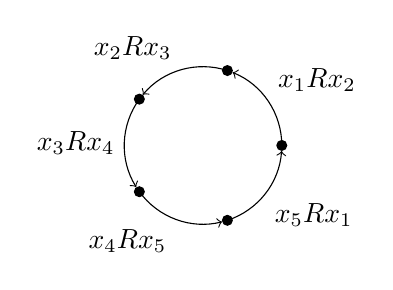
\begin{tikzpicture}
		\fill(1,0)circle(2pt)coordinate(A0);
		\fill({cos(72)},{sin(72)})circle(2pt)coordinate(A1);
		\fill({cos(144)},{sin(144)})circle(2pt)coordinate(A2);
		\fill({cos(216)},{sin(216)})circle(2pt)coordinate(A3);
		\fill({cos(288)},{sin(288)})circle(2pt)coordinate(A4);
		\begin{scope}[->]
			\draw(A0)arc[start angle=0,end angle=68,radius=1]node[midway,above right]{\(x_1 \rel{R} x_2\)};
			\draw(A1)arc[start angle=72,end angle=140,radius=1]node[midway,above left]{\(x_2 \rel{R} x_3\)};
			\draw(A2)arc[start angle=144,end angle=212,radius=1]node[midway,left]{\(x_3 \rel{R} x_4\)};
			\draw(A3)arc[start angle=216,end angle=284,radius=1]node[midway,below left]{\(x_4 \rel{R} x_5\)};
			\draw(A4)arc[start angle=288,end angle=356,radius=1]node[midway,below right]{\(x_5 \rel{R} x_1\)};
		\end{scope}
	\end{tikzpicture}
\end{center}
这是因为,如果我们有这样的环形成立,
那么根据传递性必有\(x_1 \rel{R} x_1\),
而这就与反自反性矛盾!

\begin{example}
设\(\rel{R}\)是\(A\)上的一个线性序,
证明:\(\rel{R}^{-1}\)也是\(A\)上的线性序.
\begin{proof}
由于\[
	\bigl( x \rel{R} y \land y \rel{R} z \implies x \rel{R} z \bigr)
	\iff
	\bigl( y \rel{R}^{-1} x \land z \rel{R}^{-1} y \implies z \rel{R}^{-1} x \bigr),
\]
可知\(\rel{R}^{-1}\)具有传递性.
又因为\(\rel{R}\)是\(A\)上的线性序,
所以对于\(\forall x,y \in A\),以下三个命题\[
	x \rel{R} y, \qquad
	x = y, \qquad
	y \rel{R} x
\]有且仅有一个成立;
换句话说,以下三个命题\[
	y \rel{R}^{-1} x, \qquad
	x = y, \qquad
	x \rel{R}^{-1} y
\]有且仅有一个成立;
可知\(\rel{R}^{-1}\)服从三一律.
综上所述,\(\rel{R}^{-1}\)也是\(A\)上的线性序.
\end{proof}
\end{example}


% \chapter{数系构造}
% \input{集合论/数系构造/自然数}
% \section{整数}
我们现在把自然数集扩张为整数集.
\subsection{整数集}
设\(a,b\in\omega\).
我们把数对\(\opair{a,b}\)称为“\(a\)与\(b\)的\DefineConcept{差}(difference)”,
记作\(a-b\)\footnote{读作“\(a\)减\(b\)”.},即\[
	a-b = \opair{a,b}.
\]

\begin{definition}\label{definition:集合论.自然数的差的等价关系}
%@see: 《Elements of Set Theory》 P91 Definition
我们定义\(\omega\times\omega\)上的关系\(\sim\)如下:
\[
	(\forall a,b,c,d \in \omega)
	[
		\opair{a,b} \sim \opair{c,d}
		\defiff
		a+d=b+c
	].
\]
\end{definition}

容易看出,关系\(\sim\)的定义域和值域都是自然数对.
除了通过命题公式给出\(\sim\)的定义以外,
我们还可以用更直接的形式给出它的定义:
\[
	\sim\ \defeq \Set*{
		\opair{\opair{a,b},\opair{c,d}}
		\given
		a+d=b+c \land a,b,c,d\in\omega
	}.
\]

\begin{theorem}
%@see: 《Elements of Set Theory》 P91 Theorem 5ZA
关系\(\sim\)是\(\omega\times\omega\)上的等价关系.
\begin{proof}
容易看出,关系\(\sim\)具有自反性和对称性.
现在来证\(\sim\)具有传递性.
设\[
	\opair{m,n}\sim\opair{p,q}, \qquad
	\opair{p,q}\sim\opair{r,s}.
\]
由定义有\[
	m+q=n+p, \qquad
	p+s=q+r;
\]
相加得\[
	m+q+p+s=n+p+q+r;
\]
再利用\hyperref[theorem:集合论.自然数的消去律]{消去律}便得\[
	m+s=n+r;
\]
于是\(\opair{m,n}\sim\opair{r,s}\),关系\(\sim\)具有传递性.
综上所述,关系\(\sim\)是一个等价关系.
\end{proof}
\end{theorem}

既然关系\(\sim\)是一个等价关系,
那么对于任意给定的自然数对\(\opair{m,0}\),
我们可以取得它在关系\(\sim\)下唯一的等价类\[
	[\opair{m,0}] = \Set{
		\opair{m,0},
		\opair{m+1,1},
		\opair{m+2,2},
		\dotsc
	};
\]
类似地,
对于任意给定的自然数对\(\opair{0,n}\),
我们也可以取得它在关系\(\sim\)下唯一的等价类\[
	[\opair{0,n}] = \Set{
		\opair{0,n},
		\opair{1,n+1},
		\opair{2,n+2},
		\dotsc
	}.
\]
像这样,我们把任意两个自然数\(m\)和\(n\)的差\(\opair{m,n}\)%
在关系\(\sim\)下的等价类叫做一个\DefineConcept{整数}(integer).

于是我们可以构造出“整数集”.
\begin{definition}
%@see: 《Elements of Set Theory》 P92 Definition
称“\(\omega\times\omega\)对\(\sim\)的商集”为%
\DefineConcept{整数集}(the set of integers),
记作\(\mathbb{Z}\),即\[
	\mathbb{Z} \defeq \IntegerQuotient.
\]
\end{definition}

例如,整数\(2\)是等价类\[
	[\opair{2,0}]
	= \Set{\opair{2,0},\opair{3,1},\opair{4,2},\dotsc};
\]
而整数\((-3)\)是等价类\[
	[\opair{0,3}]
	= \Set{\opair{0,3},\opair{1,4},\opair{2,5},\dotsc}.
\]

\begin{figure}[ht]
	%@see: 《Elements of Set Theory》 P92 Fig. 20. An integer is a line in \(\omega\times\omega\)
	\centering
	\begin{tikzpicture}[scale=.5]
		\draw[help lines, color=gray!30, dashed] (0,0)grid(9,9);
		\begin{scope}[>=Stealth,->]
			\draw(0,0)--(0,10);
			\draw(0,0)--(10,0);
		\end{scope}
		\foreach \i in {0,...,9} {
			\foreach \j in {0,...,9} {
				\fill (\i,\j)circle(2pt);
			}
		}
		\draw(0,4)--(5,9)node[above right]{\(-4\)};
		\draw(0,0)--(9,9)node[above right]{\(0\)};
		\draw(3,0)--(9,6)node[above right]{\(3\)};
	\end{tikzpicture}
	\caption{整数是\(\omega\times\omega\)上的“直线”}
\end{figure}

\subsection{整数集上的加法运算}
类比自然数,我们希望在整数集上也能定义加法和乘法.

利用我们从初等代数学到的知识,
容易验证下式是正确的:\[
	(m-n)+(p-q) = (m+p)-(n+q).
\]
于是我们可以定义整数集上的加法运算:
\begin{equation}\label{equation:集合论.整数集上的加法运算}
	[\opair{m,n}] + [\opair{p,q}]
	\defeq
	[\opair{m+p,n+q}].
\end{equation}
虽然已经有了整数加法的定义了,
但我们还不能确信它是良定的.
这和我们在讨论\cref{theorem:集合论.与等价关系兼容的映射的性质} 时遇到的情况是一样的.
我们想要为一对等价类给出加法运算结果的取值,就要分成下面三个步骤:
\begin{enumerate}
	\item 从两个等价类中各自取出一个代表\(\opair{m,n}\)和\(\opair{p,q}\);
	\item 在这两个代表上作运算,即\[
		\opair{m,n} + \opair{p,q}
		= \opair{m+p,n+q};
	\]
	\item 构造运算结果的等价类\([\opair{m+p,n+q}]\).
\end{enumerate}

\begin{lemma}\label{theorem:集合论.整数集上的加法运算是良定的}
%@see: 《Elements of Set Theory》 P93 Lemma 5ZB
如果\(\opair{m,n}\sim\opair{m',n'}\)且\(\opair{p,q}\sim\opair{p',q'}\),
那么\[
	\opair{m+p,n+q}\sim\opair{m'+p',n'+q'}.
\]
\begin{proof}
根据\cref{definition:集合论.自然数的差的等价关系},
\[
	m+n'=m'+n, \qquad
	p+q'=p'+q;
\]
将上述两式相加得\[
	m+p+n'+q'=m'+p'+n+q;
\]
于是\(\opair{m+p,n+q}\sim\opair{m'+p',n'+q'}\).
\end{proof}
\end{lemma}
\cref{theorem:集合论.整数集上的加法运算是良定的} 说明前面定义的%
\hyperref[equation:集合论.整数集上的加法运算]{整数集上的加法运算}是正当的.
换句话说,由于映射\[
	F\colon ((\omega\times\omega)\times(\omega\times\omega))\to(\omega\times\omega),
	\opair{\opair{m,n},\opair{p,q}} \mapsto \opair{m+p,n+q}
\]和关系\(\sim\)兼容,
那么根据\cref{theorem:集合论.与等价关系兼容的映射的性质},
在商集\(\IntegerQuotient\)上,唯一存在映射\(\hat{F}\)(这就是整数集上的加法运算),满足\[
	\hat{F}([\opair{m,n}],[\opair{p,q}]) = [\opair{m+p,n+q}].
\]

\begin{theorem}\label{theorem:集合论.整数加法的运算法则}
%@see: 《Elements of Set Theory》 P94 Theorem 5ZC
%@see: 《Elements of Set Theory》 P95 Theorem 5ZD
以下命题恒成立:
\begin{enumerate}
	\item 加法交换律
	\begin{equation}\label{equation:集合论.整数加法交换律}
		(\forall a,b\in\mathbb{Z})[a+b=b+a].
	\end{equation}
	\item 加法结合律
	\begin{equation}\label{equation:集合论.整数加法结合律}
		(\forall a,b,c\in\mathbb{Z})[(a+b)+c=a+(b+c)].
	\end{equation}
	\item 任意整数加上整数\(0\defeq[\opair{0,0}]\)不变
	\begin{equation}\label{equation:集合论.任意整数加上零不变}
		(\forall a\in\mathbb{Z})[a+0=a].
	\end{equation}
	\item 加法可逆
	\begin{equation}\label{equation:集合论.整数加法可逆}
		(\forall a\in\mathbb{Z})(\exists! b\in\mathbb{Z})[a+b=0].
	\end{equation}
\end{enumerate}
\begin{proof}
首先证明 \labelcref{equation:集合论.整数加法交换律,equation:集合论.整数加法结合律} 这两个命题.
设\[
	a = [\opair{m,n}], \qquad
	b = [\opair{p,q}], \qquad
	c = [\opair{u,v}],
\]
其中\(m,n,p,q,u,v\)是自然数.
那么\begin{align*}
	a+b &= [\opair{m,n}]+[\opair{p,q}] \\
	&= [\opair{m+p,n+q}]	\tag{\hyperref[equation:集合论.整数集上的加法运算]{整数加法的定义}} \\
	&= [\opair{p+m,q+n}]	\tag{\hyperref[equation:集合论.自然数加法交换律]{自然数加法交换律}} \\
	&= [\opair{p,q}]+[\opair{m,n}] \\
	&= b+a; \\
	(a+b)+c &= [\opair{m+p,n+q}]+[\opair{u,v}] \\
	&= [\opair{(m+p)+u,(n+q)+v}] \\
	&= [\opair{m+(p+u),n+(q+v)}]	\tag{\hyperref[equation:集合论.自然数加法结合律]{自然数加法结合律}} \\
	&= [\opair{m,n}]+[\opair{p+u,q+v}] \\
	&= a+(b+c);
\end{align*}
因此整数加法满足交换律、结合律.

命题 \labelcref{equation:集合论.任意整数加上零不变} 显然成立,
这是因为对于任意给定的整数\(a = [\opair{m,n}]\),总有\[
	a+0
	= [\opair{m,n}]+[\opair{0,0}]
	= [\opair{m+0,n+0}]
	= [\opair{m,n}]
	= a.
\]

最后,我们来证明命题 \labelcref{equation:集合论.整数加法可逆}.
显然,对于任意取定整数\(a = [\opair{m,n}]\),
整数\(b = [\opair{n,m}]\)总是满足\[
	a+b
	= [\opair{m+n,n+m}]
	= [\opair{0,0}]
	= 0.
\]
由此,我们不仅证明命题 \labelcref{equation:集合论.整数加法可逆} 中,
整数\(b\)的存在性,还给出了它的表达式.
我们再假设\(b,c\)这两个整数分别满足\[
	a+b=0, \qquad
	a+c=0;
\]
那么\[
	b=b+(a+c)=(b+a)+c=c.
\]
于是我们证得整数\(b\)的唯一性.
\end{proof}
\end{theorem}

从上面的证明过程我们得知,
对于任意给定的一个整数\(a\),
满足\(a+b=0\)的整数\(b\)存在且唯一.
于是,我们可以把\(b\)叫做“\(a\)的\DefineConcept{逆}(inverse)”,
记作\((-a)\).
那么有\begin{equation}
	-[\opair{m,n}]=[\opair{n,m}].
\end{equation}
整数的逆为我们提供了\DefineConcept{减法运算}(subtraction operation):
\begin{equation}
	b-a \defeq b+(-a).
\end{equation}

\cref{theorem:集合论.整数加法的运算法则}
说明整数集\(\mathbb{Z}\)配上加法运算就成为一个阿贝尔群!
在以后学到抽象代数的时候,我们会明白这意味着什么.

\subsection{整数集上的乘法运算}
我们遵循同样的思路,像在研究整数集上的加法运算那样,借助初等代数的知识,注意到\[
	(m-n)\cdot(p-q)=(mp+nq)-(mq+np).
\]
于是我们可以定义整数集上的乘法运算:
\begin{equation}\label{equation:集合论.整数集上的乘法运算}
	[\opair{m,n}]\cdot[\opair{p,q}]
	\defeq [\opair{mp+nq,mq+np}].
\end{equation}
同样地,我们还是要验证整数乘法的定义在等价类上是不是良定的.
也就是要验证映射\[
	G\colon ((\omega\times\omega)\times(\omega\times\omega))\to(\omega\times\omega),
	\opair{\opair{m,n},\opair{p,q}} \mapsto \opair{mp+nq,mq+np}
\]和关系\(\sim\)兼容.
为此,我们有如下引理.
\begin{lemma}\label{theorem:集合论.整数集上的乘法运算是良定的}
%@see: 《Elements of Set Theory》 P96 Lemma 5ZE
如果\(\opair{m,n}\sim\opair{m',n'}\)且\(\opair{p,q}\sim\opair{p',q'}\),
那么\[
	\opair{mp+nq,mq+np}\sim\opair{m'p'+n'q',m'q'+n'p'}.
\]
\begin{proof}
根据\cref{definition:集合论.自然数的差的等价关系},
\[
	m+n'=m'+n,
	\eqno(1)
\]\[
	p+q'=p'+q;
	\eqno(2)
\]
将(1)式乘以\(p\)倍,得\[
	mp+n'p=m'p+np;
	\eqno(3)
\]
将(1)式乘以\(q\)倍,得\[
	m'q+nq=mq+n'q;
	\eqno(4)
\]
将(2)式乘以\(m'\)倍,得\[
	m'p+m'q'=m'p'+m'q;
	\eqno(5)
\]
将(2)式乘以\(n'\)倍,得\[
	n'p'+n'q=n'p+n'q';
	\eqno(6)
\]
将(3)(4)(5)(6)这四个式子相加,
再利用\hyperref[theorem:集合论.自然数的消去律]{消去律}化简,便得\[
	mp+nq+m'q'+n'p'
	=np+mq+m'p'+n'q';
\]
因此,\(\opair{mp+nq,mq+np}\sim\opair{m'p'+n'q',m'q'+n'p'}\).
\end{proof}
\end{lemma}

\begin{theorem}\label{theorem:集合论.整数乘法的运算法则1}
%@see: 《Elements of Set Theory》 P96 Theorem 5ZF
以下命题恒成立:
\begin{enumerate}
	\item 乘法交换律
	\begin{equation}\label{equation:集合论.整数乘法交换律}
		\forall a,b\in\mathbb{Z} \bigl(
			a \cdot b = b \cdot a
		\bigr).
	\end{equation}
	\item 乘法结合律
	\begin{equation}\label{equation:集合论.整数乘法结合律}
		\forall a,b,c\in\mathbb{Z} \bigl(
			(a \cdot b) \cdot c = a \cdot (b \cdot c)
		\bigr).
	\end{equation}
	\item 乘法分配律
	\begin{equation}\label{equation:集合论.整数乘法分配律}
		\forall a,b,c\in\mathbb{Z} \bigl(
			a \cdot (b + c) = (a \cdot b) + (a \cdot c)
		\bigr).
	\end{equation}
\end{enumerate}
\begin{proof}
设\(a=[\opair{m,n}]\),\(b=[\opair{p,q}]\),其中\(m,n,p,q\in\omega\).
那么根据\cref{equation:集合论.整数集上的乘法运算},\[
	a \cdot b = [\opair{mp+nq,mq+np}],
\]\[
	b \cdot a = [\opair{pm+qn,pn+qm}].
\]
根据自然数的\hyperref[equation:集合论.自然数加法交换律]{加法交换律}%
和\hyperref[equation:集合论.自然数乘法交换律]{乘法交换律},
有\(mp+nq=pm+qn\)和\(mq+np=pn+qm\),
于是\(a \cdot b = b \cdot a\)成立.

又设\(c=[\opair{r,s}]\),其中\(r,s\in\omega\).
那么\[
	(a \cdot b) \cdot c
	= [\opair{(mp+nq)r+(mq+np)s,(mp+nq)s+(mq+np)r}],
\]\[
	a \cdot (b \cdot c)
	= [\opair{m(pr+qs)+n(ps+qr),m(ps+qr)+n(pr+qs)}].
\]
只要像上面一样,利用自然数的运算法则,
易证\((a \cdot b) \cdot c = a \cdot (b \cdot c)\).

最后,我们将\(a \cdot (b+c)\)展开,得\[
	[\opair{m(p+r)+n(q+s),m(q+s)+n(p+r)}];
\]
将\((a \cdot b) + (a \cdot c)\)展开,得\[
	[\opair{mp+nq+mr+ns,mq+np+ms+nr}].
\]
易证\(a \cdot (b + c) = (a \cdot b) + (a \cdot c)\)成立.
\end{proof}
\end{theorem}

\begin{theorem}\label{theorem:集合论.整数乘法的运算法则2}
%@see: 《Elements of Set Theory》 P97 Theorem 5ZG
以下命题恒成立:\begin{enumerate}
	\item 任意整数乘上整数\(1\defeq[(1,0)]\)不变,即
	\begin{equation}\label{equation:集合论.任意整数乘上一不变}
		\forall a\in\mathbb{Z} \bigl(
			a \cdot 1 = a
		\bigr).
	\end{equation}
	\item 整数\(1\)与整数\(0\)不相等,即\(1\neq0\).
	\item 如果\(a \cdot b = 0\),那么\(a = 0 \lor b = 0\).
\end{enumerate}
\begin{proof}
设\(a=[\opair{m,n}]\),那么
\begin{align*}
	a \cdot 1
	&= [\opair{m,n}]\cdot[(1,0)] \\
	&= [\opair{m\cdot1+n\cdot0,m\cdot0+n\cdot1}] \\
	&= [\opair{m,n}] = a.
\end{align*}
于是命题 \labelcref{equation:集合论.任意整数乘上一不变} 成立.

要证整数\(1\)与整数\(0\)不相等,
即证\([(1,0)]\neq[\opair{0,0}]\),
那么只需证\[
	\opair{0,0}\not\sim(1,0);
\]
即证\(0+0\neq0+1\)或\(0\neq1\),显然成立.

接下来,若要证\(a \cdot b = 0 \implies a = 0 \lor b = 0\),
可以用反证法,
假设\(a,b\)都是非零整数,只需证\(a \cdot b \neq 0\)制造矛盾.
设\(a=[\opair{m,n}]\),\(b=[\opair{p,q}]\),
其中\(m,n,p,q\)都是自然数.
那么\[
	a \cdot b = [\opair{mp+nq,mq+np}].
\]
既然\(a\neq0=[\opair{0,0}]\),
那么\(m \neq n\),即有\[
	m < n \lor n < m;
	\eqno(1)
\]
同理可得\[
	p < q \lor q < p.
	\eqno(2)
\]
从(1)(2)两式可以得到\(m,n,p,q\)取值的四种不同情况,不过我们总有\[
	mp+nq \neq mq+np.
\]
因此\(a \cdot b \neq 0\).
\end{proof}
\end{theorem}

我们可以说\(\opair{\mathbb{Z},+,\cdot}\)构成了%
\DefineConcept{整环}(integral domain),
这是因为\begin{enumerate}
	\item \(\opair{\mathbb{Z},+}\)构成阿贝尔群%
	(\cref{theorem:集合论.整数加法的运算法则}).
	\item 整数乘法遵守交换律和结合律,以及对加法的分配律%
	(\cref{theorem:集合论.整数乘法的运算法则1}).
	\item 整数\(1\)是乘法的单位元,且整数集中不存在零因子%
	(\cref{theorem:集合论.整数乘法的运算法则2}).
\end{enumerate}

\subsection{整数的序}
现在我们来为整数构造一个序.
利用我们从初等代数学到的知识,
容易验证下式是正确的:\[
	m-n<p-q \iff m+q<p+n.
\]
于是我们可以定义整数集上的序:
\begin{equation}\label{equation:集合论.整数集上的序}
	[\opair{m,n}] < [\opair{p,q}]
	\iff
	m+q<p+n.
\end{equation}
接下来我们想要确认这里定义的序是否不是良定的关系.

\begin{lemma}\label{theorem:集合论.整数集上的序是良定的}
%@see: 《Elements of Set Theory》 P98 Theorem 5ZH
如果\(\opair{m,n}\sim\opair{m',n'}\)且\(\opair{p,q}\sim\opair{p',q'}\),
那么\[
	m+q<p+n \iff m'+q'<p'+n'.
\]
\begin{proof}
因为\(\opair{m,n}\sim\opair{m',n'}\)且\(\opair{p,q}\sim\opair{p',q'}\),所以\[
	m+n'=m'+n, \qquad
	p+q'=p'+q.
\]
于是\begin{align*}
	m+q<p+n
	&\iff
	m+q+n'+q'<p+n+n'+q'
		\tag{\cref{theorem:集合论.自然数的加法与乘法的保序性}} \\
	&\iff
	m'+n+q+q'<p'+q+n+n'
		\tag{代入上述两个等式} \\
	&\iff
	m'+q'<p'+n'
		\tag{\cref{theorem:集合论.自然数的加法与乘法的保序性}}.
\end{align*}
\end{proof}
\end{lemma}

\begin{theorem}\label{theorem:集合论.整数集上的序是线性序}
%@see: 《Elements of Set Theory》 P98 Theorem 5ZI
关系\(<\)是整数集上的线性序.
\begin{proof}
要证关系\(<\)是整数集上的线性序,
即证\(<\)具有传递性,且满足三一律.

先证\(<\)的传递性.
考虑整数\(a=[\opair{m,n}]\),\(b=[\opair{p,q}]\),\(c=[\opair{r,s}]\),
那么\begin{align*}
	a<b \land b<c
	&\implies
	m+q<p+n \land p+s<r+q \\
	&\implies
	m+q+s<p+n+s \land p+s+n<r+q+n \\
	&\implies
	m+q+s<r+q+n \\
	&\implies
	m+s<r+n
		\tag{\cref{theorem:集合论.自然数的加法与乘法的保序性}} \\
	&\implies
	a < c.
\end{align*}

再证\(<\)服从三一律.
要说\[
	a < b, \qquad
	a = b, \qquad
	b < a
\]这三个命题中有且仅有一个成立,
等于说\[
	m+q<p+n, \qquad
	m+q=p+n, \qquad
	p+n<m+q
\]中有且仅有一个成立,
而这根据\cref{theorem:集合论.自然数集的三一律} 就能得到.
\end{proof}
\end{theorem}

\begin{definition}
设\(a\)是整数.
如果\[
	0 < a,
\]
那么称“\(a\)是\DefineConcept{正的}(\(a\) is \emph{positive})”,
或称“\(a\)是\DefineConcept{正整数}(\(a\) is a \emph{positive integer})”.
反之,如果\[
	a < 0,
\]
那么称“\(a\)是\DefineConcept{负的}(\(a\) is \emph{negative})”,
或称“\(a\)是\DefineConcept{负整数}(\(a\) is a \emph{negative integer})”.
\end{definition}

任给一个整数\(b\),
容易验证\[
	b < 0 \iff 0 < -b.
\]
于是我们又有如下的三一律:
\[
	\text{\(b\)是正的}, \qquad
	\text{\(b\)是零}, \qquad
	\text{\(-b\)是正的}
\]这三个命题有且仅有一个成立.

\begin{theorem}\label{theorem:集合论.整数的加法与乘法的保序性}
%@see: 《Elements of Set Theory》 P99 Theorem 5ZJ
设\(a,b,c\in\mathbb{Z}\).
那么\begin{gather}
	a<b \iff a+c<b+c,
	\label{equation:集合论.整数的加法的保序性} \\
	0<c \implies \bigl(
		a<b \iff a \cdot c < b \cdot c
	\bigr).
	\label{equation:集合论.整数的乘法的保序性}
\end{gather}
\begin{proof}
假设\[
	a=[\opair{m,n}], \qquad
	b=[\opair{p,q}], \qquad
	c=[\opair{r,s}].
\]
那么\cref{equation:集合论.整数的加法的保序性} 相当于\[
	m+q<p+n \iff m+r+q+s<p+r+n+s.
\]
而这根据\cref{theorem:集合论.自然数的加法与乘法的保序性} 立即可得.

要证\cref{equation:集合论.整数的乘法的保序性},
根据\cref{theorem:集合论.自然数的加法与乘法的保序性},
只需证\[
	0<c \land a<b \implies a \cdot c < b \cdot c,
\]
即证\[
	s<r \land m+q<p+n \implies mr+ns+ps+qr<pr+qs+ms+nr.
\]
如果令\(k=m+q, l=p+n\),那么上式变为\[
	s<r \land k<l \implies kr+ls<ks+lr.
\]
%TODO Exercise 25 of Chapter 4.
\end{proof}
\end{theorem}

\begin{corollary}\label{theorem:集合论.整数的消去律}
%@see: 《Elements of Set Theory》 P100 Corollary 5ZK
设\(a,b,c\in\mathbb{Z}\).
那么\begin{gather*}
	a+c=b+c \implies a=b, \\
	a \cdot c = b \cdot c \land c \neq 0 \implies a=b.
\end{gather*}
\end{corollary}
\cref{theorem:集合论.整数的消去律} 又称为“整数的消去律”.

最后,我们还可以给出减法:%@see: P101.
对于任意自然数\(m,n\),有\[
	[\opair{m,n}]=E(m)-E(n).
\]

% \section{有理数}
我们现在把整数集\(\mathbb{Z}\)扩张为有理数集\(\mathbb{Q}\).
这个过程正如我们在上一节将\(\omega\)扩张为\(\mathbb{Z}\)时一样.
实际上,从\(\mathbb{Z}\)到\(\mathbb{Q}\)的拓展体现在乘法上,
这就类似于,从\(\omega\)到\(\mathbb{Z}\)的拓展体现在加法上.
在整数集中,我们得到了加法的逆;
在有理数集中,我们希望得到乘法的逆.

\subsection{有理数集}
\begin{definition}
%@see: 《Elements of Set Theory》 P102 Definition
设\(\mathbb{Z}^* \defeq \mathbb{Z}-\{0\}\).
我们定义\(\mathbb{Z}\times\mathbb{Z}^*\)上的关系\(\sim\)如下:
\[
	(\forall a,c\in\mathbb{Z})
	(\forall b,d\in\mathbb{Z}^*)
	[
		\opair{a,b} \sim \opair{c,d}
		\defiff
		a \cdot d = c \cdot b
	].
\]

把任意一个整数\(a\)和一个非零整数\(b\)的比\(\opair{a,b}\)在关系\(\sim\)下的等价类\[
	[\opair{a,b}]
\]叫做一个\DefineConcept{分数}(fraction),
%@see: https://mathworld.wolfram.com/Fraction.html
把\(a\)称为\DefineConcept{分子}(numerator),
%@see: https://mathworld.wolfram.com/Numerator.html
把\(b\)称为\DefineConcept{分母}(denominator).
%@see: https://mathworld.wolfram.com/Denominator.html

称“\(\mathbb{Z}\times\mathbb{Z}^*\)对\(\sim\)的商集”为%
\DefineConcept{有理数集}(the set of rational numbers),
记作\(\mathbb{Q}\),即\[
	\mathbb{Q} \defeq \RationalQuotient.
\]
\end{definition}

\begin{theorem}
%@see: 《Elements of Set Theory》 P102 Theorem 5QA
关系\(\sim\)是\(\mathbb{Z}\times\mathbb{Z}^*\)上的等价关系.
\end{theorem}

\begin{figure}[htb]
	%@see: 《Elements of Set Theory》 P103Fig. 22. Rational numbers are nonhorizontal lines
	\centering
	\begin{tikzpicture}[scale=.5]
		\draw[help lines, color=gray!30, dashed] (-9,-9)grid(9,9);
		\begin{scope}[>=Stealth,->]
			\draw(0,-10)--(0,10);
			\draw(-10,0)--(10,0);
		\end{scope}
		\foreach \i in {-9,...,9} {
			\foreach \j in {-9,...,9} {
				\fill (\i,\j)circle(2pt);
			}
		}
		\draw(-3,-9)--(3,9)node[above right]{\(\tfrac{1}{3}\)};
		\draw(-5,-9)--(5,9)node[above right]{\(\tfrac{5}{9}\)};
		\draw(-9,-9)--(9,9)node[above right]{\(1\)};
		\draw(-9,-3)--(9,3)node[above right]{\(3\)};
	\end{tikzpicture}
	\caption{有理数是\(\mathbb{Z}\times\mathbb{Z}^*\)上的“直线”}
\end{figure}

\subsection{有理数集上的加法运算}
我们定义有理数集上的加法运算:
\begin{equation}\label{equation:集合论.有理数集上的加法运算}
	[\opair{a,b}]+[\opair{c,d}]=[\opair{ad+cb,bd}].
\end{equation}

\begin{lemma}\label{theorem:集合论.有理数集上的加法运算是良定的}
%@see: 《Elements of Set Theory》 P104 Lemma 5QB
如果\(\opair{a,b}\sim\opair{a',b'}\)且\(\opair{c,d}\sim\opair{c',d'}\),那么\[
	\opair{ad+cb,bd}\sim\opair{a'd'+c'b',b'd'}.
\]
\end{lemma}

\begin{theorem}\label{theorem:集合论.有理数加法的运算法则}
%@see: 《Elements of Set Theory》 P104 Theorem 5QC
以下命题恒成立:
\begin{enumerate}
	\item 加法交换律
	\begin{equation}\label{equation:集合论.有理数加法交换律}
		(\forall a,b\in\mathbb{Q})[a+b=b+a].
	\end{equation}
	\item 加法结合律
	\begin{equation}\label{equation:集合论.有理数加法结合律}
		(\forall a,b,c\in\mathbb{Q})[(a+b)+c=a+(b+c)].
	\end{equation}
	\item 任意有理数加上有理数\(0\defeq[(0,1)]\)不变
	\begin{equation}\label{equation:集合论.任意有理数加上零不变}
		(\forall a\in\mathbb{Q})[a+0=a].
	\end{equation}
	\item 加法可逆
	\begin{equation}\label{equation:集合论.有理数加法可逆}
		(\forall a\in\mathbb{Q})(\exists!b\in\mathbb{Q})[a+b=0].
	\end{equation}
\end{enumerate}
\end{theorem}

\subsection{有理数集上的乘法运算}
我们定义有理数集上的乘法运算:
\begin{equation}\label{equation:集合论.有理数集上的乘法运算}
	[\opair{a,b}]\cdot[\opair{c,d}]=[\opair{ac,bd}].
\end{equation}

\begin{lemma}\label{theorem:集合论.有理数集上的乘法运算是良定的}
%@see: 《Elements of Set Theory》 P106 Lemma 5QD
如果\(\opair{a,b}\sim\opair{a',b'}\)且\(\opair{c,d}\sim\opair{c',d'}\),那么\[
	\opair{ac,bd}\sim\opair{a'c',b'd'}.
\]
\end{lemma}

\begin{theorem}\label{theorem:集合论.有理数乘法的运算法则}
%@see: 《Elements of Set Theory》 P106 Theorem 5QE
%@see: 《Elements of Set Theory》 P107 Theorem 5QF
%@see: 《Elements of Set Theory》 P107 Corollary 5QG
以下命题恒成立:
\begin{enumerate}
	\item 乘法交换律
	\begin{equation}\label{equation:集合论.有理数乘法交换律}
		(\forall a,b\in\mathbb{Q})[a \cdot b = b \cdot a].
	\end{equation}
	\item 乘法结合律
	\begin{equation}\label{equation:集合论.有理数乘法结合律}
		(\forall a,b,c\in\mathbb{Q})[(a \cdot b) \cdot c = a \cdot (b \cdot c)].
	\end{equation}
	\item 乘法分配律
	\begin{equation}\label{equation:集合论.有理数乘法分配律}
		(\forall a,b,c\in\mathbb{Q})[a \cdot (b + c) = (a \cdot b) + (a \cdot c)].
	\end{equation}
	\item 对\(\forall r\in\mathbb{Q}^*\),\(\exists! q\in\mathbb{Q}\),使得\[
		r \cdot q = 1.
	\]
	\item 对\(\forall r,s\in\mathbb{Q}^*\),\[
		r \cdot s \neq 0.
	\]
	\item 任意有理数乘上有理数\(1\defeq[\opair{1,1}]\)不变,即
	\begin{equation}\label{equation:集合论.任意有理数乘上一不变}
		(\forall a\in\mathbb{Z})[a \cdot 1 = a].
	\end{equation}
	\item 有理数\(1\)与有理数\(0\)不相等,即\(1\neq0\).
	\item 如果\(a \cdot b = 0\),那么\(a = 0 \lor b = 0\).
\end{enumerate}
\end{theorem}

由于对于任意给定的一个非零有理数\(a\),满足\(a \cdot b = 1\)的有理数\(b\)存在且唯一.
于是,我们可以把\(b\)叫做“\(a\)的逆”,记作\(a^{-1}\).
那么有\begin{equation}
	[\opair{a,b}]^{-1}=[\opair{b,a}].
\end{equation}
有理数的逆为我们提供了\DefineConcept{除法运算}(division operation):
\begin{equation}
	s/r \defeq s \cdot (r^{-1}).
\end{equation}

我们可以说\(\opair{\mathbb{Q},+,\cdot}\)构成了\DefineConcept{有理数域}(rational field).

\subsection{有理数的序}
定义有理数集上的序:
\begin{equation}
	[\opair{a,b}]<[\opair{c,d}]
	\iff
	ad<cb.
\end{equation}

\begin{lemma}\label{theorem:集合论.有理数集上的序是良定的}
%@see: 《Elements of Set Theory》 P108 Lemma 5QH
如果\(\opair{a,b}\sim\opair{a',b'}\),
\(\opair{c,d}\sim\opair{c',d'}\),
\(b,b',d,d'\in\mathbb{Z}^+\),
那么\[
	ad<cb \iff a'd'<c'b'.
\]
\end{lemma}

\begin{theorem}\label{theorem:集合论.有理数集上的序是线性序}
%@see: 《Elements of Set Theory》 P108 Lemma 5QI
关系\(<\)是有理数集\(\mathbb{Q}\)上的线性序.
\end{theorem}

\begin{definition}
设\(r\)是有理数.
如果\[
	0<r,
\]
那么称“\(r\)是\DefineConcept{正的}”,
或称“\(r\)是\DefineConcept{正有理数}”.
反之,如果\[
	r<0,
\]
那么称“\(r\)是\DefineConcept{负的}”,
或称“\(r\)是\DefineConcept{负有理数}”.
\end{definition}

任给一个有理数\(q\),容易验证\[
	q < 0
	\iff
	0 < -q.
\]
于是我们有三一律:\[
	\text{\(q\)是正的}, \qquad
	\text{\(q\)是零}, \qquad
	\text{\(-q\)是正的}
\]这三个命题有且仅有一个成立.

我们可以定义任意有理数\(r\)的\DefineConcept{绝对值}(absolute value)为:
\begin{equation}
	\abs{r} \defeq \left\{ \begin{array}{rl}
		-r, & \text{\(-r\)是正的}, \\
		r, & \text{其他}.
	\end{array} \right.
\end{equation}

\begin{theorem}\label{theorem:集合论.有理数的加法与乘法的保序性}
%@see: 《Elements of Set Theory》 P109 Theorem 5QJ
设\(r,s,t\in\mathbb{Q}\).
\begin{gather}
	r<s \iff r+t<s+t,
	\label{equation:集合论.有理数的加法的保序性} \\
	0<t \implies \bigl(
		r<s \iff r \cdot t < s \cdot t
	\bigr).
	\label{equation:集合论.有理数的乘法的保序性}
\end{gather}
\end{theorem}

\begin{theorem}\label{theorem:集合论.有理数的消去律}
%@see: 《Elements of Set Theory》 P110 Theorem 5QK
设\(r,s,t\in\mathbb{Q}\).
那么\begin{gather*}
	r+t=s+t \implies r=s, \\
	r \cdot t = s \cdot t \land t \neq 0 \implies r=s.
\end{gather*}
\end{theorem}

% \section{实数}
古希腊毕达哥拉斯学派的数学家发现,
对于一个等腰直角三角形,
假设它的直角边都是单位长度,
要想求出它的斜边长,
仅凭有理数,显然不足以表示它.
因此我们要将有理数系进一步扩张为实数系,
这也是我们本节要着重学习的内容.

实数理论的构建可归结为完成以下三件事:\begin{enumerate}
	\item 定义无理数,将其与有理数一起组成实数系\(\mathbb{R}\).
	\item 在\(\mathbb{R}\)中定义序关系,验证这种序关系保持有理数序关系的相应性质.
	\item 在\(\mathbb{R}\)中定义四则运算,验证这些运算具有与有理数运算同样的性质.
\end{enumerate}

\subsection{实数的构造}
实际上,我们已经有了好几种方法,可以用来构造实数.
一种方式是利用十进制展开,
用一个整数和一串无限的数字序列
(相当于从\(\omega\)到\(\{0,1,2,3,4,5,6,7,8,9\}\)的映射)
来确定一个实数.

\subsubsection*{第一种途径:利用柯西列构造实数}
一种更常用的实数构造方法是
利用有理数列(即从\(\omega\)到\(\mathbb{Q}\)的映射)
去逼近一个实数,
然后把所有收敛的有理数列收集在一起,
取这个集合对一个等价关系(我们把收敛到同一个实数的两个有理数列看成是等价的)的商集.
这就是柯西用来构造实数的技巧.

\begin{definition}
%@see: 《Elements of Set Theory》 P112
设映射\(s\colon \omega\to\mathbb{Q}\)满足\[
	(\forall\epsilon\in\mathbb{Q}^+)(\exists k\in\omega)(\forall m>k)(\forall n>k)
	[\abs{s(m) - s(n)}<\epsilon],
\]
则称“\(s\)是一个\DefineConcept{柯西列}(Cauchy sequence)”.
\end{definition}

\begin{definition}
%@see: 《Elements of Set Theory》 P112
我们把全体柯西列的集合记为\(S\).
定义关系\(\sim\):\[
	r \sim s
	\defiff
	(\forall\epsilon\in\mathbb{Q}^+)(\exists k\in\omega)(\forall n>k)
	[\abs{r(n)-s(n)}<\epsilon],
\]
称“柯西列\(r\)和\(s\)等价”.
\end{definition}

可以证明关系\(\sim\)是柯西列集\(S\)上的等价关系,
以此为基础我们可以确定一个等价类划分,把它定义为实数.
\begin{definition}
%@see: 《Elements of Set Theory》 P112
称“\(S\)对\(\sim\)的商集”为\DefineConcept{实数集}(the set of real numbers),
记作\(\mathbb{R}\),即\[
	\mathbb{R} \defeq S/\kern-2pt\sim.
\]
\end{definition}
这种构造实数集的方法归功于康托.

\subsubsection*{第二种途径:利用戴德金分割构造实数}
还有一种构造实数系的方法,叫做戴德金分割.

\begin{definition}
%@see: 《数学分析(第二版 上册)》(陈纪修) P30 定义1
设有理数集\(\mathbb{Q}\)的两个非空子集\(A\)和\(B\)满足\(A \cup B = \mathbb{Q}\),
且\((\forall a\in A)(\forall b\in B)[a<b]\),
则称“\(A\)和\(B\)构成\(\mathbb{Q}\)的一个\DefineConcept{分割}”.
\end{definition}

那么从逻辑上讲,下述四种情况有且仅有一种出现:
\begin{enumerate}
	\item \(A\)有最大数\(a_0\),\(B\)没有最小数;
	\item \(A\)没有最大数,\(B\)有最小数\(b_0\);
	\item \(A\)没有最大数,\(B\)没有最小数;
	\item \(A\)有最大数\(a_0\),\(B\)有最小数\(b_0\).
\end{enumerate}
我们首先断言第四种情况是不可能发生的.
因为\(\frac{a_0+b_0}2\in\mathbb{Q}\),
且\(a_0 < \frac{a_0+b_0}2 < b_0\),
所以\(\frac{a_0+b_0}2\)既不属于\(A\),也不属于\(B\),
这就与\(\mathbb{Q}=A \cup B\)的前提矛盾.

对于第一种情况,我们称分割确定了有理数\(a_0\);
对于第二种情况,我们称分割确定了有理数\(b_0\);
对于第三种情况,分割没有确定任何有理数,在\(A\)和\(B\)之间存在一个“空隙”,
因此有必要引入“无理数”,作为这种情况下分割确定的对象.

\begin{definition}
%@see: 《Elements of Set Theory》 P113 Definition
设集合\(x \subseteq \mathbb{Q}\).
如果\begin{enumerate}
	\item \(x\)是\(\mathbb{Q}\)的非空真子集,
	即\(\emptyset \neq x \neq \mathbb{Q}\);

	\item \(x\)向下封闭(\(x\) is closed downward),
	即\[
		q \in x \land r < q \implies r \in x;
	\]

	\item \(x\)没有最大元素,
\end{enumerate}
那么称“\(x\)是一个\DefineConcept{戴德金分割}(Dedekind cut)”.
\end{definition}

应该注意到,这里没有提到等价关系,实数也不是戴德金分割的等价类,
相反地,每个戴德金分割都是一个\DefineConcept{实数}(real number).
最终,全体戴德金分割的集合就是实数集.

在戴德金分割途径下,对实数的序的定义非常简洁.
对于任意两个实数\(x\)和\(y\),定义“小于”关系\(<\):\[
	x < y \defiff x \subset y.
\]
换句话说,\[
	<\ \defeq \Set*{ \opair{x,y}\in\mathbb{R}\times\mathbb{R} \given x \subset y }.
\]

柯西法与戴德金法这两种构造实数的方法各有其优劣.
戴德金分割的优点在于:
它可以简单明了地定义实数和实数的序.
但戴德金分割的乘法却差强人意,
验证戴德金分割的乘法运算律甚是无趣.
利用柯西列构造的实数则胜在它的通用性,
这是因为它不仅仅可以用在有理数系中,
还可以用在任意的度量空间中.

“戴德金分割就是实数”
这一想法根源在于:
一个实数\(x\)可以将数轴分割为两部分,
在它左边的有理数,全都比它小.

\begin{theorem}
%@see: 《Elements of Set Theory》 P113 Theorem 5RA
关系\(<\)是实数集\(\mathbb{R}\)上的线性序.
\begin{proof}
显然关系\(<\)是传递的,于是我们只需证它满足三一律.
任取\(x,y\in\mathbb{R}\).
显然以下三个命题最多有一个成立:\[
	x \subset y, \qquad
	x = y, \qquad
	y \subset x.
\]
现在我们需要证明这三个命题中至少有一个成立.

假设前两个命题不成立,即\(x \nsubseteq y\),现在来证\(y \subset x\)必定成立.
显然\[
	x \nsubseteq y
	\implies
	(\exists r)[r \in x-y].
\]
任取\(q \in y\).
如果\(r \leq q\),
那么由定义,\(y\)向下封闭,易得\(r \in y\).
如果\(r \notin y\),
那么必有\(q < r\).
又由于\(x\)向下封闭,便得\(q \in x\).
因为\(q\)是任意取定的,而\(x \neq y\),于是可得\(y \subset x\).
\end{proof}
%@see: 《Real Analysis Modern Techniques and Their Applications Second Edition》 P5
% 我们把\(<\)和\(>\)统称为
% “\(\mathbb{R}\)的\DefineConcept{通常排序}(usual ordering)”.
% 通常排序是\(\mathbb{R}\)上的线性序.
\end{theorem}

考虑集合\(A \subseteq \mathbb{R}\).
如果实数\(x\)满足\[
	(\forall y \in A)[y \leq x],
\]
那么称“\(x\)是\(A\)的\DefineConcept{上界}(\(x\) is an \emph{upper bound} of \(A\))”.
相对地,如果实数\(x\)满足\[
	(\forall y \in A)[y \geq x],
\]
那么称“\(x\)是\(A\)的\DefineConcept{下界}(\(x\) is an \emph{lower bound} of \(A\))”.

需要注意到,\(x\)本身可能不是\(A\)的元素.

如果\[
	(\exists y\in\mathbb{R})
	[\text{\(y\)是\(A\)的上界}],
\]
那么称“\(A\)~\DefineConcept{有上界}(the set \(A\) is \emph{bounded above})”.
如果\[
	(\exists y\in\mathbb{R})
	[\text{\(y\)是\(A\)的下界}],
\]
那么称“\(A\)~\DefineConcept{有下界}(the set \(A\) is \emph{bounded below})”.

如果\(A\)的上界\(z\)比其他任何上界都要小,
即\[
	(\forall y \in \Set{ x \given \text{$x$是$A$的上界} })
	[z \leq y],
\]
那么称“\(z\)是\(A\)的\DefineConcept{最小上界}(least upper bound)”.

如果\(A\)的下界\(z\)比其他任何下界都要大,
即\[
	(\forall y \in \Set{ x \given \text{$x$是$A$的下界} })
	[z \geq y],
\]
那么称“\(z\)是\(A\)的\DefineConcept{最大下界}(greatest lower bound)”.

\begin{theorem}\label{theorem:实数.实数存在最小上界}
%@see: 《Elements of Set Theory》 P114 Theorem 5RB
实数集的任意一个有上界的非空子集总有一个实最小上界.
\end{theorem}
\cref{theorem:实数.实数存在最小上界}
指出的“实数系存在最小上界”这一性质,
是将实数域与其他有序域区分开来的重要特征.

这个定理在数学分析中也非常重要.
它可以用来证明在闭区间上的连续函数一定能取得最值.

\begin{definition}
设\(X\)是一个数系,\(<\)是\(X\)上的线性序,
\(Y\)是\(X\)的一个非空子集.
若\[
	(\forall x_1,x_2 \in X)
	(\exists y \in Y)
	[x_1 < x_2 \implies x_1 < y < x_2],
\]
则称“\(Y\)在\(X\)中是\DefineConcept{稠密的}”.
\end{definition}

\begin{proposition}
\(\mathbb{Q}\)在\(\mathbb{R}\)中是稠密的.
%@see: https://math.stackexchange.com/questions/1027970/what-does-it-mean-for-rational-numbers-to-be-dense-in-the-reals
\end{proposition}

\begin{definition}
对于\(\forall x,y\in\mathbb{R}\),
我们定义实数集上的加法运算:
\begin{equation}
	x + y \defeq \Set{
		q + r \given q \in x \land r \in y
	}.
\end{equation}
\end{definition}

\begin{lemma}
%@see: 《Elements of Set Theory》 P114 Lemma 5RC
若\(x,y\in\mathbb{R}\),那么\(x+y\in\mathbb{R}\).
\end{lemma}

\begin{theorem}
%@see: 《Elements of Set Theory》 P115 Theorem 5RD
以下命题恒成立:
\begin{enumerate}
	\item 加法交换律
	\begin{equation}
		(\forall x,y\in\mathbb{R})[x+y=y+x].
	\end{equation}
	\item 加法结合律
	\begin{equation}
		(\forall x,y,z\in\mathbb{R})[(x+y)+z=x+(y+z)].
	\end{equation}
\end{enumerate}
\end{theorem}

\begin{definition}
定义:\(0\defeq\Set{ r\in\mathbb{Q} \given r<0 }\).
\end{definition}

\begin{theorem}
%@see: 《Elements of Set Theory》 P116 Theorem 5RE
以下命题恒成立:
\begin{enumerate}
	\item \(0\)是实数.
	\item 任意实数加上实数\(0\)不变
	\begin{equation}
		(\forall x\in\mathbb{R})[x+0=x].
	\end{equation}
\end{enumerate}
\end{theorem}

\begin{definition}
%@see: 《Elements of Set Theory》 P117
设\(x\in\mathbb{R}\).
那么称集合\[
	\Set{ r \in \mathbb{Q} \given (\exists s>r) -s \notin x }
\]为“\(x\)的负元”,记作\((-x)\).
\end{definition}

\begin{theorem}
%@see: 《Elements of Set Theory》 P117 Theorem 5RF
设\(x\in\mathbb{R}\),那么\begin{enumerate}
	\item \(-x\in\mathbb{R}\).
	\item \(x+(-x)=0\).
\end{enumerate}
\end{theorem}

\begin{corollary}\label{theorem:集合论.实数的消去律}
%@see: 《Elements of Set Theory》 P118 Corollary 5RG
\((\forall x,y,z\in\mathbb{R})[
	x+z=y+z \implies x=y
]\).
\end{corollary}

\begin{theorem}\label{theorem:集合论.实数的加法的保序性}
%@see: 《Elements of Set Theory》 P118 Theorem 5RH
\((\forall x,y,z\in\mathbb{R})[
	x<y \iff x+z<y+z
]\).
\end{theorem}

\begin{definition}
%@see: 《Elements of Set Theory》 P118
设\(x\in\mathbb{R}\).
把\(x \cup -x\)称为“\(x\)的\DefineConcept{绝对值}(absolute value),
记作\(\abs{x}\),即\[
	\abs{x} \defeq x \cup -x.
\]
\end{definition}

\begin{definition}
定义:
\begin{enumerate}
	\item 如果\(x,y\)都是非负实数,那么\[
		x \cdot y
		\defeq
		0 \cup \Set{ r \cdot s \given 0 \leq r \in x \land 0 \leq s \in y }.
	\]

	\item 如果\(x,y\)都是负实数,那么\[
		x \cdot y \defeq \abs{x} \cdot \abs{y}.
	\]

	\item 如果\(x,y\)中一个是负实数一个是非负实数,那么\[
		x \cdot y \defeq -(\abs{x} \cdot \abs{y}).
	\]
\end{enumerate}
\end{definition}

\begin{definition}
定义:\(1\defeq\Set{ r\in\mathbb{Q} \given r < 1 }\).
\end{definition}

\begin{theorem}
%@see: 《Elements of Set Theory》 P119 Theorem 5RI
以下命题恒成立:
\begin{enumerate}
	\item 实数集对乘法封闭\begin{equation}
		(\forall x,y\in\mathbb{R})[x \cdot y \in \mathbb{R}].
	\end{equation}
	\item 乘法结合律\begin{equation}
		(\forall x,y,z\in\mathbb{R})[(x+y)+z=x+(y+z)].
	\end{equation}
	\item 乘法交换律\begin{equation}
		(\forall x,y\in\mathbb{R})[x+y=y+z].
	\end{equation}
	\item 乘法分配律\begin{equation}
		(\forall x,y,z\in\mathbb{R})[x\cdot(y+z)=x \cdot y+x \cdot z].
	\end{equation}
	\item \(0\neq1\).
	\item \(x\cdot1=x\).
	\item \((\forall x\in\mathbb{R}^*)(\exists y\in\mathbb{R}^*)[x \cdot y=1]\).
	\item \(0<z \implies [x<y \iff x \cdot z<y \cdot z]\).
\end{enumerate}
\end{theorem}

\subsection{区间}
定义:\begin{gather}
	(a,b) \defeq \Set{ x\in\mathbb{R} \given a<x<b }, \\
	[a,b] \defeq \Set{ x\in\mathbb{R} \given a \leq x \leq b }, \\
	(a,b] \defeq \Set{ x\in\mathbb{R} \given a < x \leq b }, \\
	[a,b) \defeq \Set{ x\in\mathbb{R} \given a \leq x < b }.
\end{gather}
我们把\([a,b]\)称为一个闭区间(closed interval),
把\((a,b)\)称为一个开区间(open interval),
把\((a,b]\)称为一个左开右闭区间,
把\([a,b)\)称为一个左闭右开区间.
%@see: https://mathworld.wolfram.com/Interval.html
%@see: https://mathworld.wolfram.com/OpenInterval.html
%@see: https://mathworld.wolfram.com/ClosedInterval.html

\subsection{确界}
\begin{definition}
%@see: 《数学分析教程(第3版 上册)》(史济怀) P40 定义1.8.1
设\(X\)是一个非空的有上界的实数的子集,
\(\beta\)是一个实数.
若\begin{itemize}
	\item \(\beta\)是\(X\)的上界,
	即\((\forall x \in X)[x \leq \beta]\),

	\item \((\forall \epsilon>0)(\exists x \in X)[x>\beta-\epsilon]\),
\end{itemize}
则称“\(\beta\)是\(X\)的\DefineConcept{上确界}(supremum)”,
记\(\sup X = \beta\).
%@see: https://mathworld.wolfram.com/Supremum.html
%@see: https://mathworld.wolfram.com/SupremumLimit.html
\end{definition}

\begin{definition}
%@see: 《数学分析教程(第3版 上册)》(史济怀) P40 定义1.8.2
设\(X\)是一个非空的有下界的实数的子集,
\(\alpha\)是一个实数.
若\begin{itemize}
	\item \(\alpha\)是\(X\)的下界,
	即\((\forall x \in X)[x \geq \alpha]\),

	\item \((\forall \epsilon>0)(\exists x \in X)[x<\alpha+\epsilon]\),
\end{itemize}
则称“\(\alpha\)是\(X\)的\DefineConcept{下确界}(infimum)”,
记\(\inf X = \alpha\).
%@see: https://mathworld.wolfram.com/Infimum.html
%@see: https://mathworld.wolfram.com/InfimumLimit.html
\end{definition}

\begin{proposition}
设\(X\)是一个非空的有上界的实数的子集,
则\(X\)的上确界就是\(X\)的最小上界.
\end{proposition}

\begin{proposition}
设\(X\)是一个非空的有下界的实数的子集,
则\(X\)的下确界就是\(X\)的最大下界.
\end{proposition}

% 如果集合\(X\)下方无界,则记\[
% 	\inf X = -\infty.
% \]
% 如果集合\(X\)上方无界,则记\[
% 	\sup X = +\infty.
% \]

\begin{theorem}[确界原理]\label{theorem:实数.确界原理}
%@see: 《数学分析教程(第3版 上册)》(史济怀) P41 定理1.8.1
%@see: 《数学分析(第二版 上册)》(陈纪修) P28 定理2.1.1(确界存在定理-实数系连续性定理)
非空的有上界的实数的子集必有上确界.
非空的有下界的实数的子集必有下确界.
\end{theorem}

\begin{theorem}
%@see: 《数学分析(第二版 上册)》(陈纪修) P29 定理2.1.2
非空的有界的实数的子集的上、下确界是唯一的.
\end{theorem}

\begin{example}\label{example:实数.确界的序}
%
证明:\begin{gather}
	\inf_{n\to\infty} a_n
	+ \inf_{n\to\infty} b_n
	\leq \inf_{n\to\infty} (a_n + b_n)
	\leq \inf_{n\to\infty} a_n
	+ \sup_{n\to\infty} b_n. \\
	\inf_{n\to\infty} a_n
	+ \sup_{n\to\infty} b_n
	\leq \sup_{n\to\infty} (a_n + b_n)
	\leq \sup_{n\to\infty} a_n
	+ \sup_{n\to\infty} b_n.
\end{gather}
%TODO
\end{example}

\subsection{有限覆盖定理}
\begingroup
\def\J{\mathscr{J}}%开区间族
\begin{definition}
%@see: 《数学分析教程(第3版 上册)》(史济怀) P43 定义1.9.1
设\(A\)是一个实数的子集,
\(\J\)是一个开区间族.
如果\[
	A \subset \bigcup \J,
\]
那么称“开区间族\(\J\)是\(A\)的一个\DefineConcept{开覆盖}”.
\end{definition}

\begin{theorem}[紧致性定理]\label{theorem:实数.紧致性定理}
%@see: 《数学分析教程(第3版 上册)》(史济怀) P43 定理1.9.1
设\([a,b]\)是一个有限闭区间,
并且它有一个开覆盖\(\J\),
那么\[
	(\exists \J')
	[
		\J' \subseteq \J
		\land
		\text{\(\J'\)是有限集}
		\land
		\text{\(\J'\)是\([a,b]\)的开覆盖}
	].
\]
\end{theorem}
\cref{theorem:实数.紧致性定理} 常被称为\DefineConcept{有限覆盖定理},
也称为\DefineConcept{海涅--波莱尔定理}.

\endgroup%end of subsection{有限覆盖定理}

% \section{基数}
\subsection{等势}
我们时不时想要研究讨论下面的问题:
两个集合是否具有相同的大小?
或者说,这两个集合的元素的个数是否相同?
还是说,一个集合相比于另一个拥有更多的元素?

\begin{definition}
%@see: 《Elements of Set Theory》 P129 Definition
设\(A,B\)都是集合.
如果存在一个从\(A\)到\(B\)的双射,
那么称“\(A\)与\(B\) \DefineConcept{等势}(\(A\) is \emph{equinumerous} to \(B\))”,
记作\(A \approx B\);
并把这个映射称为“\(A\)和\(B\)之间的\DefineConcept{一一对应}%
(\emph{one-to-one correspondence} between \(A\) and \(B\))”.
\end{definition}

\begin{example}
%@see: 《实变函数论》(周民强) P15 例2
自然数集\(\omega\)与\(\Set{ y \in \omega \given x \in \omega \land y = 2x }\)等势.
\end{example}

\begin{example}
%@see: 《Elements of Set Theory》 P129 Example
%@see: 《实变函数论》(周民强) P15 例3
自然数集\(\omega\)与\(\omega\times\omega\)等势.
这是因为映射\[
	J_1\colon \omega\times\omega\to\omega,
	\opair{m,n} \mapsto \frac12[(m+n)^2+3m+n]
\]是双射.
%@see: 《Elements of Set Theory》 P133 Exercise 1.
不止如此,映射\[
	J_2\colon \omega\times\omega\to\omega,
	\opair{m,n} \mapsto 2^m(2n+1)-1
\]也是双射.
%TODO
\end{example}

\begin{example}
%@see: 《Elements of Set Theory》 P130 Example
\(\omega\)与\(\mathbb{Q}\)等势.
%TODO
\end{example}

\begin{example}\label{example:基数.开区间与全体实数等势1}
%@see: 《Elements of Set Theory》 P130 Example
开区间\((0,1)\)与\(\mathbb{R}\)等势.
这是因为\[
	f(x) = \tan\frac{\pi(2x-1)}2
	\quad(0<x<1)
\]是从\((0,1)\)到\(\mathbb{R}\)的双射.
\end{example}

\begin{example}\label{example:基数.开区间与全体实数等势2}
%@see: 《实变函数论》(周民强) P15 例4
开区间\((-1,1)\)与\(\mathbb{R}\)等势.
这是因为\[
	f(x) = \frac{x}{1-x^2}
	\quad(-1<x<1)
\]是从\((-1,1)\)到\(\mathbb{R}\)的双射.
\end{example}

\begin{example}\label{example:基数.幂集与特征函数空间等势}
%@see: 《Elements of Set Theory》 P131 Example
证明:对于任意集合\(A\),
总有\(A\)的幂集\(\Powerset A\)与映射空间\(2^A\)等势.
\begin{proof}
对于\(A\)的每个子集\(a\),
定义从\(A\)到\(\{0,1\}\)的映射\[
	f_a(x) = \left\{ \begin{array}{cl}
		1, & x \in a, \\
		0, & x \in A - a.
	\end{array} \right.
\]
注意到\(2=\{0,1\}\),
于是\(f_a \in 2^A\).
再定义映射\[
	H\colon \Powerset A \to 2^A,
	a \mapsto f_a.
\]
对于\(\forall a,b \in \Powerset A\),
只要\(a \neq b\),
就\(\exists x \in A\),
满足\(x \in a\),但不满足\(x \in b\),
这就使得\(f_a(x) = 1\)而\(f_b(x) = 0\),
于是\(f_a \neq f_b\),
由此可见\(H\)是单射.
又因为对于\(\forall g \in 2^A\),
若记\(G = \Set{ x \in A \given g(x) = 1 }\),
则必有\((\forall x \in A - G)[g(x) = 0]\),
于是\(H(G) = g\),
即\(g \in \ran H\).
由\(g\)的任意性可知\(\ran H = 2^A\),
因此\(H\)是满射.
既然\(H\)是双射,那么\(\Powerset A \approx 2^A\).
\end{proof}
\end{example}

\begin{example}
全体完全平方数组成的集合与自然数集\(\omega\)等势.
\end{example}

\begin{example}
全体偶数组成的集合与整数集\(\mathbb{Z}\)等势.
\end{example}

\begin{theorem}\label{theorem:集合论.等势相当于等价关系}
%@see: 《Elements of Set Theory》 P132 Theorem 6A
对于任意集合\(A,B,C\):\begin{enumerate}
	\item \(A \approx A\).
	\item \(A \approx B \implies B \approx A\).
	\item \(A \approx B \land B \approx C \implies A \approx C\).
\end{enumerate}
\end{theorem}
\cref{theorem:集合论.等势相当于等价关系}
说明\DefineConcept{等势}(equinumerosity)
和每一个等价关系都一样,
也具有自反性、对称性、传递性,
但要注意,它不是一个等价关系,
这是因为它关注的是全体集合.

\begin{theorem}
%@see: 《Elements of Set Theory》 P132 Theorem 6B(a)
自然数集\(\omega\)与实数集\(\mathbb{R}\)不等势.
\end{theorem}

\begin{theorem}
%@see: 《Elements of Set Theory》 P132 Theorem 6B(b)
没有集合与它的幂集等势.
\end{theorem}

\subsection{有限集,无限集}
\begin{definition}
%@see: 《Elements of Set Theory》 P133 Definition
设\(A\)是集合.
当且仅当存在自然数\(n\)与之等势时,
称“\(A\)是\DefineConcept{有限的}(finite)”
或“\(A\)是\DefineConcept{有限集}”;
否则称“\(A\)是\DefineConcept{无限的}(infinite)”
或“\(A\)是\DefineConcept{无限集}”,
即\begin{gather}
	\text{\(A\)是有限的}
	\defiff
	(\exists n\in\omega)[A \approx n]; \\
	\text{\(A\)是无限的}
	\defiff
	(\forall n\in\omega)\neg[A \approx n].
\end{gather}
\end{definition}

\begin{example}
任一自然数是有限集.
\end{example}

\subsection{鸽巢原理}
\begin{theorem}[鸽巢原理]
%@see: 《Elements of Set Theory》 P134 Pigeonhold Principle
没有自然数与它的真子集等势.
\end{theorem}

\begin{corollary}
%@see: 《Elements of Set Theory》 P135 Corollary 6C
没有有限集与它的真子集等势.
\end{corollary}

\begin{corollary}
%@see: 《Elements of Set Theory》 P136 Corollary 6D
任一集合,如果与其真子集等势,就是无限的.
\end{corollary}

\begin{corollary}
%@see: 《Elements of Set Theory》 P136 Corollary 6E
任一集合总与唯一一个自然数等势.
\end{corollary}

\subsection{基数}
\begin{definition}
设\(A\)是有限集.
满足\(A \approx n\)的自然数\(n\),
称为“\(A\)的\DefineConcept{基数}(cardinal number)\footnote{%
有的地方也将其称为\DefineConcept{元数}或\DefineConcept{浓度}.}”,
记作\(\card A\)或\(\abs{A}\).
\end{definition}

\begin{example}
\((\forall n\in\omega)[\card n = n]\).
\end{example}

我们可以看出,对于任意两个有限集\(A\)和\(B\),
我们有\(A \approx \card A\)和\[
	\card A = \card B
	\iff
	A \approx B.
\]

从\cref{example:基数.幂集与特征函数空间等势} 可以推出任一有限集的所有子集的个数.
\begin{theorem}
设\(A\)是有限集,
则\begin{equation}
	\card \Powerset A
	= 2^{\card A}.
\end{equation}
\end{theorem}

\begin{lemma}
%@see: 《Elements of Set Theory》 P137 Lemma 6F
如果\(C\)是自然数\(n\)的真子集,
那么存在\(m<n\)使得\(C \approx m\).
\end{lemma}

\begin{theorem}
%@see: 《Elements of Set Theory》 P137 Corollary 6G
任一有限集的任一子集也是有限的.
\end{theorem}

\subsection{基数算术}
\begin{definition}
%@see: 《Elements of Set Theory》 P139 Definition
设\(A,B\)都是集合,
\(\card A = \alpha\),
\(\card B = \beta\).
\begin{enumerate}
	\item 如果\(A\)和\(B\)互斥,那么\(\card(A \cup B)=\alpha+\beta\).
	\item \(\card(A \times B)=\alpha\cdot\beta\).
	\item \(\card(A^B)=\alpha^\beta\).
\end{enumerate}
\end{definition}

需要注意到的是,
如果给定的两个集合\(A,B\)不互斥,
那么可以令\[
	A' = A\times\{0\}, \qquad
	B' = B\times\{1\},
\]
从而有\(A' \approx A\),\(B' \approx B\),
以及\(A'\)和\(B'\)互斥.

\begin{theorem}
%@see: 《Elements of Set Theory》 P139 Theorem 6H
设\(A \approx B\),\(C \approx D\).
\begin{enumerate}
	\item 如果\(A \cap C = B \cap D = \emptyset\),
	那么\(A \cup C \approx B \cup D\).
	\item \(A \times C \approx B \times D\).
	\item \(A^C \approx B^D\).
\end{enumerate}
\end{theorem}

\begin{theorem}
%@see: 《Elements of Set Theory》 P144 Corollary 6K
如果\(A,B\)都是有限集,
那么\[
	A \cup B, \qquad
	A \times B, \qquad
	A^B
\]也都是有限的.
\end{theorem}

\subsection{基数排序}
我们可以利用等势的概念来判定两个集合的大小是否一致,
但是我们要怎么说明一个集合比另一个集合更大呢?

\begin{definition}
%@see: 《Elements of Set Theory》 P145 Definition
设\(A,B\)都是集合.
当且仅当存在从\(A\)到\(B\)的单射,
称“\(A\)由\(B\) \DefineConcept{主导}(\(A\) is \emph{dominated} by \(B\))”,
记作\(A \preceq B\)或\(B \succeq A\).
\end{definition}

\begin{example}
\(A \preceq A\).
\end{example}

\begin{example}
\(A \subseteq B \implies A \preceq B\).
\end{example}

\begin{theorem}
\(A \preceq B
\iff
(\exists b)[b \subseteq B \implies A \approx b]\).
\end{theorem}

\begin{definition}
设\(A,B\)都是集合.
定义:\begin{equation}
	\card A \leq \card B \defiff A \preceq B.
\end{equation}
\end{definition}

\begin{proposition}
设映射\(f\colon A \to B\),
则\begin{align*}
	\text{$f$是单射}
	\implies
	\card A \leq \card B, \\
	\text{$f$是满射}
	\implies
	\card A \geq \card B, \\
	\text{$f$是双射}
	\implies
	\card A = \card B.
\end{align*}
\end{proposition}

\begin{lemma}\label{theorem:基数.集合在映射下的分解}
%@see: 《实变函数论》(周民强) P15 引理1.4
设映射\(f\colon A \to B,
g\colon B \to A\),
则存在集合\(X_1,X_2,Y_1,Y_2\),
使得\begin{enumerate}
	\item \(\{X_1,X_2\}\)是\(A\)的一个划分,
	\(\{Y_1,Y_2\}\)是\(B\)的一个划分,
	\item \(X_1\)在\(f\)下的像为\(f\ImageOfSetUnderRelation{X_1}=Y_1\),
	\(Y_2\)在\(g\)下的像为\(g\ImageOfSetUnderRelation{Y_2}=X_2\).
\end{enumerate}
\begin{proof}
我们首先作出如下定义:
设\(E\)是\(A\)的一个子集(不妨假定\(B - f\ImageOfSetUnderRelation{E} \neq \emptyset\)),
若\[
	E \cap g\ImageOfSetUnderRelation{B - f\ImageOfSetUnderRelation{E}} = \emptyset,
	\eqno(1)
\]
则称“\(E\)是\(A\)中的\DefineConcept{分离集}”.

现将\(A\)中的分离集的全体记为\(\Gamma\).
令\(X_1 = \bigcup \Gamma\).
我们有\(X_1 \in \Gamma\).%TODO 为什么?
事实上,
对于\(\forall E \in \Gamma\),
由于\(X_1 \supseteq E\),
故从(1)式可知\(E \cap g\ImageOfSetUnderRelation{B - f\ImageOfSetUnderRelation{X_1}} = \emptyset\),
从而有\(X_1 \cap g\ImageOfSetUnderRelation{B - f\ImageOfSetUnderRelation{X_1}} = \emptyset\).
这说明\(X_1\)不光是\(A\)中的分离集,而且是\(\Gamma\)中对包含关系\(\subseteq\)的最大元.

现在令\(f\ImageOfSetUnderRelation{X_1}=Y_1,
B-Y_1=Y_2,
g\ImageOfSetUnderRelation{Y_2}=X_2\).
首先知道\(B=Y_1 \cup Y_2\).
其次,由于\(X_1 \cap X_2 = \emptyset\),
故又易得\(X_1 \cup X_2 = A\).
事实上,若不然,那么\(\exists a \in A\),
使得\(a \notin X_1 \cup X_2\).
现在取\(X_3 = X_1 \cup \{a\}\),
我们有\[
	Y_1 = f\ImageOfSetUnderRelation{X_1} \subseteq f\ImageOfSetUnderRelation{X_3},
	\qquad
	Y_2 \supseteq B - f\ImageOfSetUnderRelation{X_3},
\]
从而知\(X_2 \supseteq g\ImageOfSetUnderRelation{B - f\ImageOfSetUnderRelation{X_3}}\).
这就是说\[
	X_1 \cap g\ImageOfSetUnderRelation{B - f\ImageOfSetUnderRelation{X_3}} = \emptyset.
\]
由此可得\[
	X_3 \cap g\ImageOfSetUnderRelation{B - f\ImageOfSetUnderRelation{X_3}} = \emptyset.
\]
这与“\(X_1\)是\(\Gamma\)的最大元”相矛盾!
\end{proof}
\end{lemma}
\cref{theorem:基数.集合在映射下的分解} 是由巴拿赫建立的.

\begin{theorem}\label{theorem:集合论.施罗德--伯恩斯坦定理}
%@see: 《Elements of Set Theory》 P147 Schroder-Bernstein Theorem(a)
%@see: 《实变函数论》(周民强) P16 定理1.5
设\(A,B\)都是集合,则\[
	A \preceq B \land B \preceq A \implies A \approx B.
\]
\begin{proof}
根据定义可知,
存在单射\(f\colon A \to B\)和\(g\colon B \to A\).
根据\hyperref[theorem:基数.集合在映射下的分解]{映射分解定理}知\[
	A = X_1 \cup X_2, \qquad
	B = Y_1 \cup Y_2, \qquad
	f\ImageOfSetUnderRelation{X_1} = Y_1, \qquad
	f\ImageOfSetUnderRelation{Y_2} = X_2.
\]
因为\(f\)和\(g^{-1}\)是双射,
所以我们可以构造一个从\(A\)到\(B\)的双射:\[
	h(x) = \left\{ \begin{array}{cl}
		f(x), & x \in X_1, \\
		g^{-1}(x), & x \in X_2,
	\end{array} \right.
\]
这就说明\(A \approx B\).
\end{proof}
\end{theorem}
\cref{theorem:集合论.施罗德--伯恩斯坦定理}
常被称为“施罗德--伯恩斯坦定理”,
不过有时候也被称为“康托--伯恩斯坦定理”.
最先是康托于1897年证明了该定理,
但是他的证明利用了一条等价于选择公理的原理.
后来,施罗德在他于1896年撰写的一篇摘要中发表了这条定理,
但是他给出的证明是有缺陷的.
菲利克斯·伯恩斯坦是第一个为这条定理给出完全令人满意的证明的人,
波莱尔把他的证明发表在自己于1898年出版的
《函数论讲义(Le\c{c}ons sur la th\'eorie des fonctions)》上.
但是这里对\cref{theorem:集合论.施罗德--伯恩斯坦定理} 的证明是由巴拿赫给出的.

利用\cref{theorem:集合论.施罗德--伯恩斯坦定理} 可以得到如下推论.
\begin{corollary}\label{theorem:集合论.施罗德--伯恩斯坦定理.推论1}
%@see: 《Elements of Set Theory》 P148 Examples 1.
设\(A,B,C\)是集合,
且\(A \subseteq B \subseteq C\).
若\(A \approx C\),
则\(B \approx C\).
\end{corollary}

\begin{example}\label{example:基数.闭区间与全体实数等势1}
%@see: 《Elements of Set Theory》 P148 Examples 2.
因为\((-1,1)\subseteq[-1,1]\subseteq\mathbb{R}\),
且\((-1,1)\approx\mathbb{R}\),
所以\([-1,1]\approx\mathbb{R}\).

因为\((0,1)\subseteq[0,1]\subseteq\mathbb{R}\),
且\((0,1)\approx\mathbb{R}\),
所以\([0,1]\approx\mathbb{R}\).
\end{example}
在\cref{example:基数.闭区间与全体实数等势1} 中,
我们如果要直接建立\([-1,1]\)与\(\mathbb{R}\)之间的一一对应,就会比较繁琐.
这是因为想用一个连续函数来表示所需的一一对应是不可能的,
在以后我们会学到,闭区间上的连续函数的值域仍是闭区间(\cref{theorem:极限.最值定理}).
不过,只要运用\cref{theorem:集合论.施罗德--伯恩斯坦定理.推论1}
以及\cref{example:基数.开区间与全体实数等势2} 的结论,
就可以间接证明\([-1,1]\)与\(\mathbb{R}\)等势.

\begin{proposition}
%@see: 《Real Analysis Modern Techniques and Their Applications Second Edition》 P7 0.9 Proposition
设\(A\)是集合,
则\[
	\card A < \card(\Powerset A).
\]
\end{proposition}

\begin{example}
%@see: 《Elements of Set Theory》 P148 Examples 4.
\(\mathbb{R}\approx2^\omega\),
\(\mathbb{R}\approx\Powerset\omega\).
\end{example}

\subsection{可数集,不可数集}
\begin{definition}
%@see: 《Real Analysis Modern Techniques and Their Applications Second Edition》 P7
设\(A\)是集合.
若\[
	\card A \leq \card\mathbb{N},
\]
则称“\(A\)是\DefineConcept{可数的}(countable, denumerable)”.
反之,若\[
	\card A > \card\mathbb{N},
\]
则称“\(A\)是\DefineConcept{不可数的}(uncountable)”.
\end{definition}

\begin{proposition}
%@see: 《Real Analysis Modern Techniques and Their Applications Second Edition》 P7
有限集是可数的.
任一有限集\(A\)的基数\(\card A\)等于它的元素个数.
\end{proposition}

\begin{definition}
%@see: 《Real Analysis Modern Techniques and Their Applications Second Edition》 P7
若集合\(A\)既是无限的又是可数的,
则称“\(A\)是\DefineConcept{可数无限的}(countably infinite)”.
\end{definition}

\begin{proposition}
%@see: 《Real Analysis Modern Techniques and Their Applications Second Edition》 P8 0.10 Proposition
如果集合\(A,B\)都是可数的,
那么\(A \times B\)也是可数的.
\end{proposition}

\begin{proposition}
%@see: 《Real Analysis Modern Techniques and Their Applications Second Edition》 P8 0.10 Proposition
如果
\begin{enumerate}
	\item 集合\(A\)是可数的;
	\item 对于每个\(a \in A\),\(X_a\)都是可数的,
\end{enumerate}
那么\(\bigcup_{a \in A} X_a\)是可数的.
\end{proposition}

\begin{proposition}
%@see: 《Real Analysis Modern Techniques and Their Applications Second Edition》 P8 0.10 Proposition
如果集合\(A\)是可数无限的,
那么\(\card A = \card{N}\).
\end{proposition}

\begin{corollary}
%@see: 《Real Analysis Modern Techniques and Their Applications Second Edition》 P8 0.11 Corollary
\(\mathbb{Z}\)是可数的.
\end{corollary}

\begin{corollary}
%@see: 《Real Analysis Modern Techniques and Their Applications Second Edition》 P8 0.11 Corollary
\(\mathbb{Q}\)是可数的.
\end{corollary}

\begin{proposition}
%@see: 《Real Analysis Modern Techniques and Their Applications Second Edition》 P8 0.12 Proposition
\(\card(\Powerset\mathbb{N}) = \card\mathbb{R}\).
\end{proposition}

\begin{corollary}
%@see: 《Real Analysis Modern Techniques and Their Applications Second Edition》 P8 0.13 Corollary
设\(A\)是集合.
如果\(\card A \geq \card\mathbb{R}\),
那么\(A\)是不可数的.
\end{corollary}

\begin{proposition}
%@see: 《Real Analysis Modern Techniques and Their Applications Second Edition》 P9 0.14 Proposition
设\(A,B\)都是集合.
若\(\card A \leq \card\mathbb{R}\)且\(\card B \leq \card\mathbb{R}\),
则\(\card(A \times B) \leq \card\mathbb{R}\).
\end{proposition}

\begin{proposition}
%@see: 《Real Analysis Modern Techniques and Their Applications Second Edition》 P9 0.14 Proposition
如果
\begin{enumerate}
	\item \(\card A \leq \card\mathbb{R}\);
	\item \[
		(\forall a \in A)
		[\card X_a \leq \card\mathbb{R}],
	\]
\end{enumerate}
那么\[
	\card\left( \bigcup_{a \in A} X_a \right) \leq \card\mathbb{R}.
\]
\end{proposition}


\part{初等数学}
\chapter{算术与代数}

\section{比}
\subsection{比例数}
\begin{definition}
给定两个数\(a\)和\(b\),
如果数\(c\)满足\(a=b \cdot c\),
则称“\(c\)是\(a\)与\(b\)的\DefineConcept{比例数}(简称\DefineConcept{比})”,
记作\(a \propto b\)或\(a:b=c\)或\(a/b=c\)或\(\frac{a}{b}=c\),
并称\(a\)和\(b\)为这个比的\DefineConcept{项},
称\(a\)为\DefineConcept{前项},
称\(b\)为\DefineConcept{后项}.
\end{definition}

\begin{property}
\(\frac{a}{b} = \frac{ma}{mb}\ (m\neq0)\).
\end{property}

\begin{definition}
相对于比\(a:b\),比\(a^2:b^2\)称为\(a:b\)的\DefineConcept{二次比},
\(a^3:b^3\)称为\(a:b\)的\DefineConcept{三次比},
\(a^{\frac{1}{2}}:b^{\frac{1}{2}}\)称为\(a:b\)的\DefineConcept{平方根比}.
\end{definition}

\begin{example}
设\[
	\frac{a}{b} = \frac{c}{d} = \frac{e}{f} = \dotsb = k,
\]
证明:\[
	\left(
		\frac{
			p a^n + q c^n + r e^n + \dotsb
		}{
			p b^n + q d^n + r f^n + \dotsb
		}
	\right)^{\frac1n} = k,
\]
其中\(p,q,r,\dotsc\)和\(n\)都是任意常数.
\end{example}

\begin{example}
已知\(\frac{a}{b}=\frac{c}{d}=\frac{e}{f}\),
证明:\(\frac{a^3b+2c^2e-3ae^2f}{b^4+2d^2f-3bf^3} = \frac{ace}{bdf}\).
%TODO
\end{example}

\begin{example}
已知\(\frac{x}{a}=\frac{y}{b}=\frac{z}{c}\),
证明:\[
	\frac{x^2+a^2}{x+a}+\frac{y^2+b^2}{y+b}+\frac{z^2+c^2}{z+c}
	= \frac{(x+y+z)^2+(a+b+c)^2}{x+y+z+a+b+c}.
\]
%TODO
\end{example}

\begin{example}
已知方程\(7x=4y+8z, 3z=12x+11y\),求比\(x:y:z\).
\begin{solution}
方程移项,得\begin{gather*}
	7x-4y-8z=0, \\
	12x+11y-3z=0,
\end{gather*}
从每个方程的第二项开始写出系数,并利用“交叉相乘法”
\[
	\begin{array}{*4r}
		-4, & -8, & 7, & -4, \\
		11, & -3, & 12, & 11,
	\end{array}
\]
得到\begin{gather*}
	(-4)\times(-3)-11\times(-8)=100, \\
	(-8)\times12-(-3)\times7=-75, \\
	7\times11-12\times(-4)=125,
\end{gather*}
即\[
	\frac{x}{100}=\frac{y}{-75}=\frac{z}{125}
	\quad\text{或}\quad
	\frac{x}{4}=\frac{y}{-3}=\frac{z}{5}.
\]
\end{solution}
\end{example}

\subsection{比例}
\begin{definition}
给定四个数\(a,b,c,d\),
如果有\(\frac{a}{b}=\frac{c}{d}\),
则称“\(a,b,c,d\)是\DefineConcept{成比例的}”,
记作\[
	a:b = c:d,
\]
并称\(a\)和\(d\)两项为\DefineConcept{外项},
称\(b\)和\(c\)为\DefineConcept{内项}.
\end{definition}

显然,当数\(a,b,c,d\)成比例时,
\(\frac{a}{b}=\frac{c}{d}\),
必有\(b,d\)均不为零,于是\[
	bd \cdot \frac{a}{b} = bd \cdot \frac{c}{d},
\]\[
	ad = bc,
\]
也就是说,“外项之积等于内项之积.”

\begin{definition}
如果数\(a,b,c,d,\dotsc\)满足\[
	\frac{a}{b} = \frac{b}{c} = \frac{c}{d} = \dotsb,
\]
则称“\(a,b,c,d,\dotsc\)成\DefineConcept{连比}”.

特别地,当\(a,b,c\)成连比(即\(a:b = b:c\))时,
称\(b\)为\DefineConcept{比例中项},
称\(c\)为\(a\)与\(b\)的\DefineConcept{第三比例项}.
\end{definition}

我们有以下几个平凡的结论:\begin{enumerate}
	\item 若\(\frac{a}{b} = \frac{b}{c}\),
	则\(\frac{a}{c} = \frac{a^2}{b^2}\).
	\item 若\(\frac{a}{b} = \frac{c}{d}\)
	且\(\frac{e}{f} = \frac{g}{h}\),
	则\(\frac{ae}{bf} = \frac{cg}{dh}\).
	\item {\bf 交等定理}\footnote{%
	交等定理、反比定理、交比定理、合比定理、分比定理和合分比定理
	这几个名称实际上取自欧几里得的《几何原本》.%
	}.
	若\(\frac{a}{b} = \frac{c}{d}\)
	且\(\frac{b}{x} = \frac{d}{y}\),
	则\(\frac{a}{x} = \frac{c}{y}\).
	\item {\bf 反比定理}.
	若\(\frac{a}{b} = \frac{c}{d}\),
	则\(\frac{b}{a} = \frac{d}{c}\).
	\item {\bf 交比定理}.
	若\(\frac{a}{b} = \frac{c}{d}\),
	则\(\frac{a}{c} = \frac{b}{d}\).
	\item {\bf 合比定理}.
	若\(\frac{a}{b} = \frac{c}{d}\),
	则\((a+b):b = (c+d):d\).
	\item {\bf 分比定理}.
	若\(\frac{a}{b} = \frac{c}{d}\),
	则\((a-b):b = (c-d):d\).
	\item {\bf 合分比定理}.
	若\(\frac{a}{b} = \frac{c}{d}\),
	则\(\frac{a+b}{a-b} = \frac{c+d}{c-d}\).
\end{enumerate}

\begin{example}
解方程\[
	\frac{\sqrt{x+1}+\sqrt{x-1}}{\sqrt{x+1}-\sqrt{x-1}} = \frac{4x-1}{2}.
\]
\begin{solution}
注意到原方程中\(x\)的取值范围是\(x\geq1\).
利用合分比定理,有\[
	\frac{\sqrt{x+1}}{\sqrt{x-1}} = \frac{4x+1}{4x-3},
\]
所以\[
	\frac{x+1}{x-1} = \frac{16x^2+8x+1}{16x^2-24x+9}.
\]
再利用合分比定理,有\[
	\frac{2x}{2} = \frac{32x^2-16x+10}{32x-8},
\]
即\[
	x = \frac{16x^2-8x+5}{16x-4},
\]
解得\(x=\frac{5}{4} \geq1\).
\end{solution}
\end{example}

\subsection{变化率}
\begin{definition}
已知互相关联的两个量\(A\)与\(B\).
如果每当\(B\)变化了,就有\(A\)也随之变化一个相同的比率,
那么称“量\(A\)与量\(B\)成\DefineConcept{正比}”,
记作\(A \propto B\).
\end{definition}

\begin{theorem}
如果\(A\)与\(B\)成正比,那么\(A\)等于\(B\)乘以一个常量.
\begin{proof}
设数\(\AutoTuple{a}{0}\)和\(\AutoTuple{b}{0}\)是\(A\)和\(B\)的对应的取值.
根据定义,有\[
	\def\f#1{%
		\frac{a_#1}{a_1} = \frac{b_#1}{b_1}%
	}
	\f2,\f3,\f4,\dotsc,
\]
于是\[
	\def\f#1{\frac{a_#1}{b_#1}}
	\frac{A}{B} = \f1 = \f2 = \f3 = \f4 = \dotsb.
	\qedhere
\]
\end{proof}
\end{theorem}

\begin{definition}
已知两个量\(A\)与\(B\).
如果\(A\)与\(B\)的倒数成正比,
那么称“量\(A\)与量\(B\)成\DefineConcept{反比}”.
\end{definition}

结合“正比”与“反比”的定义,如果\(A\)同\(B/C\)成正比,
那么称“\(A\)同\(B\)成正比,而同\(C\)成反比”.

\section{整式}
我们把用运算符号把数和表示数的字母连接而成的式子叫做\DefineConcept{代数式}.
运算符号是指加、减、乘、除、乘方、开方、绝对值、括号等符号.
代数式中不允许出现等号、不等号.

由数与字母的积组成的代数式叫做\DefineConcept{单项式}(monomial).
%@see: https://mathworld.wolfram.com/Monomial.html
例如\[
	1, \qquad
	a, \qquad
	4b^2, \qquad
	7abc
\]都是单项式.
单项式中的数叫做这个单项式的\DefineConcept{系数}(coefficient).
例如\(a\)的系数是\(1\),
\(4b^2\)的系数是\(4\),
而\(7abc\)的系数是\(7\).
在一个单项式中,所有字母的次数的和,叫做这个单项式的次数.
上面的四个单项式的次数分别是\(0\)次、\(1\)次、\(2\)次和\(3\)次.

由几个单项式的和组成的代数式叫做\DefineConcept{多项式}(polynomial).
%@see: https://mathworld.wolfram.com/Polynomial.html
多项式中的每个单项式叫做这个多项式的\DefineConcept{项}(term),
其中不含字母的项叫做这个多项式的\DefineConcept{常数项}(constant term).
例如\[
	1+a, \qquad
	b+2c^2+\frac12cde,
\]都是多项式.
在一个多项式中,次数最高的项的次数,就是这个多项式的\DefineConcept{次数}.
上面的两个多项式的次数分别是\(1\)次和\(3\)次.

只含一种字母的多项式,叫做\DefineConcept{一元多项式}(univariate polynomial).
%@see: https://mathworld.wolfram.com/UnivariatePolynomial.html
含有两种字母的多项式,叫做\DefineConcept{二元多项式}(bivariate polynomial).
%@see: https://mathworld.wolfram.com/BivariatePolynomial.html
含有两种以上字母的多项式,统称为\DefineConcept{多元多项式}(multivariate polynomial).

系数全是整数的多项式,叫做\DefineConcept{整系数多项式}(integer polynomial).
%@see: https://mathworld.wolfram.com/IntegerPolynomial.html
系数全是有理数的多项式,叫做\DefineConcept{有理系数多项式}(rational polynomial).
%@see: https://mathworld.wolfram.com/RationalPolynomial.html
系数全是实数的多项式,叫做\DefineConcept{实系数多项式}(real polynomial).
%@see: https://mathworld.wolfram.com/RealPolynomial.html
系数全是复数的多项式,叫做\DefineConcept{复系数多项式}(complex polynomial).
%@see: https://mathworld.wolfram.com/ComplexPolynomial.html

我们把单项式和多项式统称为\DefineConcept{整式}.

通常我们会把一个多项式按其中某一字母的次数按从小到大或从大到小的顺序排列起来.
当我们按从小到大的顺序排列时,叫做“把多项式按字母升幂排列”.
当我们按从大到小的顺序排列时,叫做“把多项式按字母降幂排列”.

在多项式中,我们把所含字母相同,且相同字母的次数也相同的项,叫做\DefineConcept{同类项}.
为了简化记号,方便思考,我们常常会把多项式中的同类项合并成一项;
具体来说,就是把同类项的系数相加,所得结果作为新的项的系数,同时保持原来的项的字母及其次数不变.
例如\(1\)和\(4\)是同类项,
\(a\)和\(3a\)是同类项,
\(4b^2\)和\(7b^2\)是同类项,
\(7abc\)和\(13abc\)是同类项.
%
\begingroup
\chapter{初等数论}
数论在一些地方总有让人意想不到的妙用.
有这样一种说法:“自然科学的皇后是数学,数学的皇冠是数论,哥德巴赫猜想则是皇冠上的明珠.”
在这一章,我们介绍一些基础的数论理论,供大家参考.

\section{素数与合数}
在正整数集上,由于没有引入负数、分数的概念,
正整数\(x\)与\(y\)相除的结果除了商\(z\)以外,
还经常是带有余数\(r\)的,于是有关系式\[
	x = y z + r.
\]

\begin{definition}
在正整数集上,如果\(x\)与\(y\)相除余\(r=0\),
我们就称“\(y\)可以\DefineConcept{整除} \(x\)”
或“\(x\)可以被\(y\)整除”
或“\(x\)是\(y\)的\DefineConcept{倍数}”
或“\(y\)是\(x\)的\DefineConcept{因子}”,
记作\(\truediv{x}{y}\),
即\[
	\truediv{x}{y}
	\defiff
	(\exists z \in \mathbb{N}^+)
	[x = y z].
\]
\end{definition}

\begin{definition}
设\(a,b\in\mathbb{N}^+\).
\(a\)与\(b\)的\DefineConcept{最大公约数}(greatest common divisor),记作\((a,b)\);
\(a\)与\(b\)的\DefineConcept{最小公倍数}(least common multiple),记作\([a,b]\).
\end{definition}
在本章以外,为了防止最大公约数、最小公倍数记号与开区间、闭区间符号混淆,
分别记作\(\gcd{p,q}\)和\(\lcm{p,q}\).

\begin{theorem}
设\(a,b\in\mathbb{N}^+\).
已知\(a\)与\(b\)的最大公约数\((a,b)\)和最小公倍数\([a,b]\),
那么\((a,b)\times[a,b]=ab\).
\end{theorem}

\begin{definition}
如果正整数\(x\)只能被1或它自己整除\footnote{特别地,我们规定1不是素数.},
那么称\(x\)为\DefineConcept{素数}或\DefineConcept{质数}(prime number);
否则称之为\DefineConcept{合数}(composite number).
\end{definition}
这就是说:\[
	\text{$x$是素数}
	\defiff
	(\forall y)(\forall z)
	[y \cdot z=x \implies y=1 \lor z=1].
\]

\begin{definition}
如果正整数\(x\)与\(y\)除了1以外没有其他公因子,
就称“\(x\)与\(y\) \DefineConcept{互素}(或\DefineConcept{互质})”.
\end{definition}

全体素数的集合,
记作\(\mathbb{S}\),
即\[
	\mathbb{S}
	\defeq
	\Set*{
		x\in\mathbb{N}^+-\{1\}
		\given
		(\forall y\in\mathbb{N}^+)
		[y \neq x \implies (x,y)=1]
	}.
\]

\begin{theorem}
如果一个正整数\(a\)能整除正整数的乘积\(bc\),且\(a\)与其中一个因子\(b\)互素,
则\(a\)必能整除另一个因子\(c\).
\end{theorem}
\begin{corollary}
如果素数\(a\)能整除正整数的乘积\(bcd\dotsm\),则\(a\)必能整除该乘积的一个因子.
\end{corollary}
\begin{corollary}
如果素数\(a\)能整除正整数的乘积\(b^n\ (n\in\mathbb{N}^+)\),那么\(a\)必能整除\(b\).
\end{corollary}

\begin{theorem}
如果正整数\(a\)与正整数\(b,c\)均互素,则它必与乘积\(bc\)互素.
\end{theorem}
\begin{corollary}
如果正整数\(a\)与正整数的乘积\(bc\)互素,则\(a\)与正整数\(b,c\)均互素.
\end{corollary}
\begin{corollary}
如果正整数\(a\)与\(b\)互素,则\(a^m\ (m\in\mathbb{N}^+)\)与\(b^n\ (n\in\mathbb{N}^+)\)互素.
\end{corollary}

\begin{theorem}
如果正整数\(a\)与\(b\)互素,则分数\(\frac{a^m}{b^n}\ (m,n\in\mathbb{N}^+)\)均为既约分数.
\end{theorem}
\begin{corollary}
设\(a,b,c,d\in\mathbb{N}^+\).
如果\(\frac{a}{b} = \frac{c}{d}\),
且\(\frac{a}{b}\)是既约分数,
则\[
	(\forall k\in\mathbb{R}^*)
	[c = ka, d = kb].
\]
\end{corollary}

不难发现,第一个素数是2,它也是素数中唯一一个偶数.
第二个素数是3,接下来是5、7、11……
我们不禁发问,素数的个数究竟是有限的,还是无限的.
\begin{theorem}
素数有无穷多个,
即\[
	(\forall x)(\exists y)[y>x \land \text{$y$是素数}].
\]
\begin{proof}
用反证法\footnote{这个证法是由古希腊数学家欧几里得给出的.}.
假设素数只有\(k\)个,分别是\(\AutoTuple{p}{k}\),且\(p_1 < p_2 < \dotsb < p_k\).
显然,数\(\truediv{p_1 p_2 \dotsm p_k}{p_i}\ (i=1,2,\dotsc,k)\).
但数\[
	N = 1 + p_1 p_2 \dotsm p_k
\]与\(p_i\ (i=1,2,\dotsc,k)\)相除总余1,
这就说明数\(N\)要么是一个素数,
要么是一个可以被区间\((p_k,N)\)内的一个正整数\(M\)整除的合数,
总之素数的个数大于\(k\).
以此类推,可知素数必然有无穷多个.
\end{proof}
\end{theorem}

\begin{theorem}
没有任何一个有理代数式能唯一地表示素数.
\begin{proof}
用反证法.
假设有理代数式\[
p(x) = a_0 + a_1 x + a_2 x^2 + \dotsb
\]唯一地表示素数,且\[
p(m) = a_0 + a_1 m + a_2 m^2 + \dotsb = q.
\]但\begin{align*}
p(m+nq) &= a_0 + a_1 (m+nq) + a_2 (m+nq)^2 + \dotsb \\
&= a_0 + a_1 m + a_2 m^2 + \dotsb + \alpha q \quad(\alpha\in\mathbb{Q}) \\
&= q + \alpha q = (1+\alpha)q,
\end{align*}即\(\truediv{p(m+nq)}{q}\),说明\(p(m+nq)\)不是一个素数.
\end{proof}
\end{theorem}

\begin{theorem}
一个数只能以一种方式分解素因子.
\begin{proof}
设合数\(N\)可以分解为乘积\(abcd\dotsm\),其中\(a,b,c,d,\dotsc\)是素数;又设\(N = \alpha\beta\gamma\delta\dotsm\),其中\(\alpha,\beta,\gamma,\delta,\dotsc\)是另一些素数;那么\[
abcd\dotsm = \alpha\beta\gamma\delta\dotsm.
\]
显然,数\(\alpha\)可以整除\(abcd\dotsm\),所以\(\alpha\)至少能整除它们中的一个因子,不妨设\(\truediv{a}{\alpha}\),但是由于\(a,b,c,d,\dotsc\)都是素数,故可知\(a=\alpha\),因此\[
bcd\dotsm = \beta\gamma\delta\dotsm.
\]以此类推,最后得到\(b=\beta,c=\gamma,d=\delta,\dotsc\),也就是说,任意合数的素因子分解式是唯一的.
\end{proof}
\end{theorem}

\begin{example}
已知合数\(N = a^p b^q c^r \dotsm\),其中\(a,b,c,\dotsc\)是不同的素数,\(p,q,r,\dotsc\)是正整数.
计算\(N\)的因子个数,\(N\)分解成两个因子的方式数,\(N\)分解成两个互素的因子的方式数,\(N\)的所有因子之和.
\begin{solution}
因为乘积\[
(1+a+a^2+\dotsb+a^p)
(1+b+b^2+\dotsb+b^q)
(1+c+c^2+\dotsb+c^r)\dotsm
\]的展开式的每一项都是数\(N\)的一个因子,
所以,\(N\)的因子个数%
\footnote{这里“因子个数”包括了1和合数\(N\)本身.}%
就是上述乘积的项数\((p+1)(q+1)(r+1)\dotsm\).

当\(N\)不是完全平方数时,\(N\)分解成两个因子的方式显然有\[
\frac{1}{2} (p+1)(q+1)(r+1)\dotsm
\]种.

当\(N\)是完全平方数时,\(N = \sqrt{N}\times\sqrt{N}\)也是一种分解方式,但对应于这种分解方式的因子只有一个\(\sqrt{N}\).
如果不计入这种分解方式,那么\(N\)的分解方式有\[
\frac{1}{2} \left[-1 + (p+1)(q+1)(r+1)\dotsm\right]
\]种;再加上刚刚提到的一种特殊分解方式\(N = \sqrt{N}\times\sqrt{N}\),那么\(N\)的分解方式总共有\[
\frac{1}{2} \left[1 + (p+1)(q+1)(r+1)\dotsm\right]
\]种.

在将数\(N\)分解成互素的两个因子\(\alpha,\beta\)时,其中一个必须包含\(a^p\),否则就会有\(a\)的一些幂在一个因子中,\(a\)的另一些幂在在另一个因子中,于是这两个因子就不互素了.
以此类推,可知“\(N\)分解成两个互素的因子的方式数”与“\(abcd\dotsm\)分解成两个因子的方式数”相等,即为\[
\frac{1}{2}(1+1)(1+1)(1+1)\dotsm.
\]若设\(N\)中共有\(n\)个不同的素因子,那么\(N\)分解成两个互素的因子的方式数是\[
\frac{1}{2} \cdot 2^n = 2^{n-1}.
\]

如前所述,由于乘积\[
(1+a+a^2+\dotsb+a^p)
(1+b+b^2+\dotsb+b^q)
(1+c+c^2+\dotsb+c^r)\dotsm
\]展开式的每一项都是一个因子,所以“\(N\)的所有因子之和”就等于这个乘积,由等比数列的求和公式,便得\(N\)的所有因子之和为\[
\frac{1-a^{p+1}}{1-a}\cdot\frac{1-b^{q+1}}{1-b}\cdot\frac{1-c^{r+1}}{1-c}\dotsm.
\]
\end{solution}
\end{example}

\section{费马小定理}
\begin{lemma}\label{theorem:初等数论.费马小定理.引理0}
证明:任意\(r\)个连续正整数的乘积能被\(r!\)整除.
\begin{proof}
设从正整数\(n\)开始的连续\(r\)个正整数的乘积为\(P_n = n(n+1)(n+2)\dotsm(n+r-1)\),那么\[
P_{n+1} = (n+1)(n+2)\dotsm(n+r),
\]\[
n P_{n+1} = (n+r) P_n = n P_n + r P_n,
\]\[
P_{n+1} = P_n + \frac{r}{n} P_n,
\]\[
P_{n+1} - P_n = r \frac{P_n}{n},
\]上式等号右边是\(r-1\)个连续正整数的\(r\)倍.
因此,如果任意\(r-1\)个连续正整数的乘积能被\((r-1)!\)整除,就有\(P_{n+1} - P_n\)能被\(r!\)整除.
因为\(P_1 = 1 \cdot 2 \dotsm r = r!\),所以\(P_2\)必是\(r!\)的倍数,从而\(P_3,P_4,\dotsc\)也都是\(r!\)的倍数.
这样就证明了“如果\(r-1\)个连续正整数的乘积能被\((r-1)!\)整除,那么\(r\)个连续正整数的乘积便能被\(r!\)整除”.
但是由于每两个连续正整数(必有一个奇数和一个偶数)的乘积能被\(2!=2\)整除,所以每三个连续正整数的乘积也能被\(3!\)整除;以此类推,该命题普遍成立.
\end{proof}
\end{lemma}

\begin{lemma}\label{theorem:初等数论.费马小定理.引理1}
设\(p\)是素数.
证明:除了第一项和最后一项以外,\((a+b)^p\)展开式的每一项的系数,都可以被\(p\)整除.
\begin{proof}
除了第一项与最后一项以外的各项系数为\[
C_p^r = \frac{p(p-1)(p-2)\dotsm(p-r+1)}{r!},
\]其中\(r=1,2,\dotsc,p-1\).
因为\(p\)是素数,所以\(r!\)中(除了1以外)没有一个因子可以整除\(p\);
又因为\(p>r\),所以\(p\)也不能整除\(r!\)中的任一因子;
也就是说,\((p-1)(p-2)\dotsm(p-r+1)\)必能被\(r!\)整除,而系数\(C_p^r\)必能被\(p\)整除.
\end{proof}
\end{lemma}

\begin{lemma}\label{theorem:初等数论.费马小定理.引理2}
设\(p\)是素数.
证明:\[
(a+b+c+d+\dotsb)^p = M + a^p + b^p + c^p + d^p + \dotsb,
\]其中\(M\)是\(p\)的倍数.
\begin{proof}
记\(\beta=b+c+\dotsb\),则由\cref{theorem:初等数论.费马小定理.引理1} 可知\[
(a+\beta)^p = a^p + \beta^p + M_1,
\]其中\(M_1\)是\(p\)的倍数.
接下来,记\(\gamma=c+d+\dotsb\),则同样有\[
\beta^p = (b+\gamma)^p = b^p + \gamma^p + M_2,
\]其中\(M_2\)是\(p\)的倍数.
以此类推,便得要证的结果,且\(M = M_1+M_2+\dotsb\).
\end{proof}
\end{lemma}

\begin{theorem}[费马小定理]\label{theorem:初等数论.费马小定理}
如果\(p\)是素数,且正整数\(n\)与\(p\)互素,则\(n^{p-1}-1\)是\(p\)的倍数.
\begin{proof}
根据\cref{theorem:初等数论.费马小定理.引理2},在\(n\)个正整数的和的\(p\)次幂\[
(a+b+c+d+\dotsb)^p = M + a^p + b^p + c^p + d^p + \dotsb
\]中令\(a=b=c=d=\dotsb=1\),那么有\[
n^p = n + M
\quad\text{或}\quad
n^p - n = n(n^{p-1}-1) = M,
\]即\(\truediv{n^{p-1}-1}{p}\).
\end{proof}
\end{theorem}

\begin{corollary}
如果\(p\)是素数,且\(p\neq2\),那么\(p-1\)是偶数,且对于任意正整数\(N\)总有\[
\left(N^{\frac{p-1}{2}}+1\right)
\left(N^{\frac{p-1}{2}}-1\right)
\]是\(p\)的倍数,或者说\[
N^{\frac{p-1}{2}} = Kp\pm1,
\]其中\(K\)是某个正整数.
\end{corollary}

\begin{corollary}[费马小定理']
如果\(p\)是素数,则\(\truediv{n^p-n}{p}\).
\end{corollary}

\begin{example}
设\(p\)是素数,证明:任意两个正整数的\(p\)次幂的差比这两个数的差大\(p\)的倍数.
\end{example}

\begin{example}
证明:任意完全平方数要么等于\(5n\),要么等于\(5n\pm1\),其中\(n\in\mathbb{N}^+\).
\end{example}

\begin{example}[费马猜想]
费马提出过一个错误的猜想:数\(2^{2^n}+1\ (n=0,1,2,\dotsc)\)都是素数.
这个猜想在当\(n=0,1,2,3,4\)时是正确的,但很遗憾的是,数学家欧拉发现,当\(n=5\)时,数\(2^{2^5}+1 = 4294967297 = 641 \times 6700417\)是合数.
% Mathematica: FactorInteger[2^(2^5)+1]
\end{example}

\section{无理数}
\begin{proposition}
设\(n\in\mathbb{N}^+\),且\(n\)不是完全平方数,则\(\sqrt{n}\)是无理数.
\begin{proof}
用反证法.
假设\(\sqrt{n} = p/q\),其中\(p,q\in\mathbb{N}^+\).
由于\(n\)不是完全平方数,故有\(m\in\mathbb{N}^+\),使得\(m<p/q<m+1\),
从而\(mq<p<mq+q\),\(0<p-mq<q\).
在等式\(p^2=nq^2\)的两边都减去\(mpq\),
得到\(p^2-mpq=nq^2-mpq\),
提取公因式得\(p(p-mq)=q(nq-mp)\),
整理得\[
	\frac{p}{q} = \frac{nq-mp}{p-mq}.
\]
令\(p_1=nq-mp\),\(q_1=p-mq\).
由于\(q_1\in\mathbb{N}^+\)且\(q_1<q\),
所以\(p_1\in\mathbb{N}^+\)且\(p_1<p\).
对等式\[
	\frac{p}{q} = \frac{p_1}{q_1}
\]反复地进行同样的讨论,
可以得出两串递减的正整数列\[
	p>p_1>p_2>p_3>\dotsb
	\quad\text{与}\quad
	q>q_1>q_2>q_3>\dotsb,
\]
使得\[
	\frac{p}{q}=\frac{p_1}{q_1}=\frac{p_2}{q_2}=\frac{p_3}{q_3}=\dotsb.
\]
这是不可能的,因为从\(p\)或\(q\)开始的正整数不可能无止境地递减下去.
这就证明了\(\sqrt{n}\)不可能是有理数.
\end{proof}
\end{proposition}
\endgroup

\chapter{复数概论}
\section{复数的形式与运算}
\subsection{复数的代数形式}
\begin{definition}[虚数单位]
规定:满足\(\iu^2=-1\)的数\(\iu\)称为\DefineConcept{虚数单位}.
\end{definition}

\begin{definition}
把由有序实数对\((x,y)\)作代数组合所确定的数\(z=x+\iu y\)称为代数形式的\DefineConcept{复数}.
实数\(x\)、\(y\)分别称为复数\(z=x+\iu y\)的\DefineConcept{实部}、\DefineConcept{虚部},记作\(x=\Re z\)、\(y=\Im z\).

特别地,当\(\Im z=0\)时,\(z=\Re z=x\)是实数;
当\(\Re z=0\)时,\(z=\iu\Im z=\iu y\),称为\DefineConcept{纯虚数}.
\end{definition}

\begin{definition}[代数形式下复数相等条件]
设\(z_1\)和\(z_2\)都是复数,则当\(\Re z_1 = \Re z_2\)和\(\Im z_1 = \Im z_2\)同时成立时,则称\(z_1 = z_2\).
特别地,对于复数\(z\),则当且仅当\(\Re z=0\)且\(\Im z=0\)时,\(z=0\).
\end{definition}

\begin{definition}[共轭复数]
设\(z=x + \iu y \in\mathbb{C}\),其中\(x,y\in\mathbb{C}\),称复数\(\complexconjugate{z}=x - \iu y\)为\(z\)的\DefineConcept{共轭复数}(conjugate).
\end{definition}

\subsection{复数的模}
\begin{definition}[复数的模]
设复数\(z = x + \iu y\),称\[
\abs{z} = \sqrt{x^2 + y^2}
\]为\(z\)的\DefineConcept{模}或\DefineConcept{绝对值}.
\end{definition}

\begin{property}
共轭复数以及复数的模具有以下性质:
\begin{enumerate}
\item \(\Re \complexconjugate{z} = \Re z\);
\item \(\Im \complexconjugate{z} = -\Im z\);
\item \(\complexconjugate{(\complexconjugate{z})} = z\);
\item \(z+\complexconjugate{z} = 2 \Re z\);
\item \(z-\complexconjugate{z} = 2\iu \Im z\);
\item \(z\complexconjugate{z} = \abs{z}^2\);
\item \(\abs{\complexconjugate{z}}=\abs{z}\);
\item \(\abs{z_1 z_2} = \abs{z_1} \abs{z_2}\);
\item \(\abs{\frac{z_1}{z_2}} = \frac{\abs{z_1}}{\abs{z_2}} \quad(z_2 \neq 0)\);
\item \(\complexconjugate{z_1 \pm z_2} = \complexconjugate{z_1} \pm \complexconjugate{z_2}\);
\item \(\complexconjugate{z_1 z_2} = \complexconjugate{z_1} \cdot \complexconjugate{z_2}\);
\item \(\complexconjugate{\left(\frac{z_1}{z_2}\right)} = \frac{\complexconjugate{z_1}}{\complexconjugate{z_2}} \quad (z_2 \neq 0)\);
\item \(-\abs{z} \leq \Re z \leq \abs{z} \leq \abs{\Re z} + \abs{\Im z}\);
\item \(-\abs{z} \leq \Im z \leq \abs{z} \leq \abs{\Re z} + \abs{\Im z}\).
\end{enumerate}
\end{property}

\subsection{复数的代数运算}
\begin{definition}[复数加法]
设\(z_1=x_1+\iu y_1\),\(z_2=x_2+\iu y_2\),
定义\[
z_1+z_2=(x_1+x_2)+\iu(y_1+y_2)
\]为复数\(z_1\)和\(z_2\)的加法运算.
\end{definition}

\begin{definition}[复数减法]
设\(z_1=x_1+\iu y_1\),\(z_2=x_2+\iu y_2\),定义\[
z_1-z_2=(x_1-x_2)+\iu(y_1-y_2)
\]为复数的\(z_1\)和\(z_2\)的减法运算.
显然,复数减法是加法的逆运算.
\end{definition}

\begin{definition}[复数乘法]
设\(z_1 = x_1 + \iu y_1\),\(z_2 = x_2 + \iu y_2\),定义\[
z_1 \cdot z_2
= (x_1 + \iu y_1)(x_2 + \iu y_2)
= (x_1 x_2 - y_1 y_2)+\iu(x_1 y_2 + x_2 y_1)
\]为复数\(z_1\)和\(z_2\)的乘法运算.
\end{definition}

\begin{definition}[复数除法]
设\(z_1 = x_1 + \iu y_1\),\(z_2 = x_2 + \iu y_2 \neq 0\),定义满足\[
z_1 = z \cdot z_2
\]的复数\(z = x + \iu y\)为复数\(z_1\)和\(z_2\)的商,记作\[
z = \frac{z_1}{z_2},
\]称为复数\(z_1\)和\(z_2\)的除法运算.

显然,复数的除法是乘法的逆运算.
\end{definition}

\begin{theorem}
设\(z_1 = x_1 + \iu y_1\),\(z_2 = x_2 + \iu y_2 \neq 0\),则\[
\frac{z_1}{z_2}
= \frac{z_1 \cdot \complexconjugate{z_2}}{z_2 \cdot \complexconjugate{z_2}}
= \frac{z_1 \cdot \complexconjugate{z_2}}{\abs{z_2}^2}
= \frac{x_1 x_2 + y_1 y_2}{x_2^2 + y_2^2}
+ \iu \frac{x_2 y_1 - x_1 y_2}{x_2^2 + y_2^2}.
\]
\begin{proof}
设\(z = x + \iu y = \frac{z_1}{z_2}\),则\[
z \cdot z_2 = (x + \iu y)(x_2 + \iu y_2)
= (x_2 x - y_2 y) + \iu(y_2 x + x_2 y)
= x_1 + \iu y_1,
\]从而有方程组\[
\left\{ \begin{array}{l}
x_2 x - y_2 y = x_1, \\
y_2 x + x_2 y = y_1,
\end{array} \right.
\]解得\[
x = \frac{x_1 x_2 + y_1 y_2}{x_2^2 + y_2^2},
\quad
y = \frac{x_2 y_1 - x_1 y_2}{x_2^2 + y_2^2}.
\]
\end{proof}
\end{theorem}

\begin{theorem}
若\(z,w \in \mathbb{C}\),则有\begin{equation}
\abs{z \pm w}^2 = \abs{z}^2 + \abs{w}^2 \pm 2 \Re(z \complexconjugate{w}).
\end{equation}
\begin{proof}
\(
\abs{z + w}^2
= (z + w) (\complexconjugate{z + w})
= z\complexconjugate{z} + z\complexconjugate{w} + w\complexconjugate{z} + w\complexconjugate{w}
= \abs{z}^2 + 2 \Re(z\complexconjugate{w}) + \abs{w}^2
\).
\end{proof}
\end{theorem}

\begin{theorem}
若\(z,w \in \mathbb{C}\),则有\begin{equation}
\abs{z + w}^2 \leq (\abs{z} + \abs{w})^2.
\end{equation}
\begin{proof}
\(
\abs{z + w}^2
= \abs{z}^2 + 2 \Re(z \complexconjugate{w}) + \abs{w}^2
\leq \abs{z}^2 + 2 \abs{z}\abs{\complexconjugate{w}} + \abs{w}^2
= (\abs{z} + \abs{w})^2
\).
\end{proof}
\end{theorem}

\begin{theorem}[三角不等式]
若\(z,w \in \mathbb{C}\),则有\begin{equation}
\abs{\abs{z}-\abs{w}} \leq \abs{z \pm w} \leq \abs{z} + \abs{w}.
\end{equation}
\begin{proof}
因为\[
\abs{z + w}^2 \leq (\abs{z} + \abs{w})^2,
\]所以\(\abs{z + w} \leq \abs{z} + \abs{w}\).

又因为\[
\abs{z} = \abs{z + w + (-w)} \leq \abs{z+w} + \abs{-w} = \abs{z+w} + \abs{w},
\]所以\(\abs{z}-\abs{w} \leq \abs{z+w}\).

同样地,有\(\abs{w}-\abs{z} \leq \abs{z+w}\).

综上所述,\(\abs{\abs{z}-\abs{w}}\leq\abs{z+w}\).
\end{proof}
\end{theorem}

\begin{example}
证明:\(\abs{z_1+z_2}^2 + \abs{z_1-z_2}^2 = 2 (\abs{z_1}^2 + \abs{z_2}^2)\).
\begin{proof}
记\(z_1 = x_1 + \iu y_1, z_2 = x_2 + \iu y_2\).那么\[
z_1+z_2 = (x_1+x_2) + \iu(y_1+y_2),
\]\[
\abs{z_1+z_2}^2 = (x_1+x_2)^2 + (y_1+y_2)^2;
\]同理\(\abs{z_1-z_2}^2 = (x_1-x_2)^2 + (y_1-y_2)^2\).那么\begin{align*}
\abs{z_1+z_2}^2 + \abs{z_1-z_2}^2
&= (x_1+x_2)^2 + (y_1+y_2)^2
+ (x_1-x_2)^2 + (y_1-y_2)^2 \\
&= 2 ( x_1^2 + x_2^2 + y_1^2 + y_2^2 )
= 2 ( \abs{z_1}^2 + \abs{z_2}^2 ).
\qedhere
\end{align*}
\end{proof}
\end{example}

\subsection{复数的几何表示}
\begin{definition}[复数在复平面上的几何表示]
在直角坐标系\(xOy\)上可以用点\((x,y)\)表示复数\(z=x+\iu y\),
也可以用向量\((x,y)\)表示复数\(z=x+\iu y\).
与复数建立了这种对应关系的坐标平面\(xOy\)称为\DefineConcept{复平面}(complex plane),
%@see: https://mathworld.wolfram.com/ComplexPlane.html
记作\(C\).
称\(x\)轴为复平面的\DefineConcept{实轴}(real axis).
%@see: https://mathworld.wolfram.com/RealAxis.html
%@see: https://mathworld.wolfram.com/RealLine.html
称\(y\)轴为复平面的\DefineConcept{虚轴}(imaginary axis).
%@see: https://mathworld.wolfram.com/ImaginaryAxis.html
%@see: https://mathworld.wolfram.com/ImaginaryLine.html

显然,表示复数\(z\)的点与表示其共轭复数\(\complexconjugate{z}\)的点关于实轴对称.
\end{definition}

\begin{definition}[复数在复球面上的几何表示]
在\(Ox_1x_2x_3\)坐标系下,考虑单位球面\(S\)(即球心位于原点、半径为1的球面):\[
	x_1^2+x_2^2+x_3^2=1
\]
点\((0,0,1)\)称为北极,记作\(N\),
同时\(x_1Ox_2\)平面取为复平面\(C\).
复平面\(C\)交球面\(S\)于单位球的赤道.

对于复平面\(C\)上的每一个点\(z\),它与\(N\)连接的直线必与\(S\)交且只交于一点\(Z \neq N\).
若\(\abs{z} < 1\),则点\(Z\)在下半球面上;
若\(\abs{z} > 1\),则点\(Z\)在上半球面上;
若\(\abs{z} = 1\),则点\(Z\)在赤道上.
反之,取球面上任意一点\(Z \neq N\),连接它与\(N\)的直线也只与复平面\(C\)交于一点\(z\).

可见,除北极\(N=(0,0,1)\)以外,复平面\(C\)和球面\(S\)上的点是一一对应的.
并且当\(\abs{z} \to +\infty\)时,\(Z \to N\).
那么可以假想一个模为无穷大的复数,
称作\DefineConcept{无穷远点}(point at infinity),
%@see: https://mathworld.wolfram.com/PointatInfinity.html
%@see: https://mathworld.wolfram.com/ComplexInfinity.html
记作\(z = \infty\),
作为复平面\(C\)上与复球面北极\(N\)对应的点.

加上无穷远点后的复平面称为\DefineConcept{扩充复平面}(extended complex plane),
%@see: https://mathworld.wolfram.com/ExtendedComplexPlane.html
记作\(C_\infty\),即\[
C_\infty = C \cup \{\infty\}.
\]
扩充复平面\(C_\infty\)又称为\DefineConcept{闭平面}.
对应地,复平面\(C\)因为不含无穷远点,所以又称为\DefineConcept{开平面}.

复球面\(S\)与扩充复平面\(C_\infty\)上点之间的映射称为\DefineConcept{球极射影}.
\(S\)又称为\DefineConcept{黎曼复球面}(Riemann sphere).
%@see: https://mathworld.wolfram.com/RiemannSphere.html

另外,对于\(\infty\)还有以下几点值得注意:
\begin{enumerate}
\item \(\infty\)的实部\(\Re\infty\)、虚部\(\Im\infty\)、辐角\(\Arg\infty\)均无意义,其模\(\abs{\infty}=+\infty\);
\item 运算\(\infty \pm \infty\)、\(0 \cdot \infty\)、\(\frac{\infty}{\infty}\)均无意义;
\item 设复数\(z \neq \infty\),有\(z \pm \infty = \infty \pm z = \infty\),\(\frac{z}{\infty} = 0\);
\item 设复数\(z \neq 0\),有\(z \cdot \infty = \infty \cdot z = \infty\),\(\frac{z}{0} = \infty\);
\item 设复数\(z \neq 0\)且\(z \neq \infty\),有\(\frac{\infty}{z} = \infty\);
\item 在扩充复平面\(C_\infty\)上,任一直线都是通过无穷远点\(\infty\)的.同时,没有一个半平面包含点\(\infty\).
\end{enumerate}
\end{definition}

\begin{theorem}
设复数\(z=x+\iu y\),其对应的复球面上的点为\(Z=\opair{x_1,x_2,x_3}\),并满足:

当\(z \neq \infty\)时,\(Z\)的坐标为\[
x_1 = \frac{z + \complexconjugate{z}}{\abs{z}^2 + 1}, \qquad
x_2 = \iu\frac{\complexconjugate{z} - z}{\abs{z}^2 + 1}, \qquad
x_3 = \frac{\abs{z}^2 - 1}{\abs{z}^2 + 1}
\]或\[
x_1 = \frac{2x}{x^2+y^2+1}, \quad
x_2 = \frac{2y}{x^2+y^2+1}, \quad
x_3 = \frac{x^2+y^2-1}{x^2+y^2+1}.
\]

当\(z = \infty\)时,\(Z\)的坐标为\(N = (0,0,1)\).
\end{theorem}

\begin{theorem}
已知复球面上一点\(Z=(x_1,x_2,x_3)\),则其对应的复平面上的点为\[
z = x+\iu y = \frac{x_1+\iu x_2}{1-x_3}
\]
\end{theorem}


\chapter{函数}
\section{函数的概念}
\subsection{一元函数的概念}
设\(D\)是\(\mathbb{R}\)的一个非空子集,
称映射\(f\colon D \to \mathbb{R}\)为
“定义在\(D\)上的一个\DefineConcept{一元函数}(univariate function)”,
%@see: https://mathworld.wolfram.com/UnivariateFunction.html
简称\DefineConcept{函数},通常记为\[
	y = f(x), \qquad x \in D,
\]
其中点集\(D\)称为该函数的\DefineConcept{定义域},
\(x\)称为\DefineConcept{自变量},
\(y\)称为\DefineConcept{因变量}.

函数定义中,对每个\(x \in D\),
按对应法则\(f\),总有唯一确定的值\(y\)与之相应,
这个值称为函数\(f\)在\(x\)处的\DefineConcept{函数值},
记作\(f(x)\),即\(y=f(x)\).
因变量\(y\)与自变量\(x\)之间的这种依赖关系,通常称为\DefineConcept{函数关系}.
函数值\(f(x)\)的全体所构成的集合称为函数\(f\)的\DefineConcept{值域},
记作\(R_f\)或\(f\ImageOfSetUnderRelation{D}\),即\[
	R_f = f\ImageOfSetUnderRelation{D} = \Set{ y \given y = f(x) \land x \in D }.
\]

函数的定义域通常按以下两种情形来确定:
\begin{itemize}
	\item 一种是对有实际背景的函数,
	根据实际背景中变量的实际意义来确定.
	\item 另一种是对抽象地用算式表达的函数,
	通常约定这种函数的定义域是使得算式有意义的一切实数组成的集合,
	这种定义域称为函数的\DefineConcept{自然定义域}.
\end{itemize}

\begin{example}
函数\(y = \frac{1}{x}\)的自然定义域是
\(\Set{ x \in \mathbb{R} \given x \neq 0 }\).
\end{example}

\begin{example}
函数\(y = \sqrt{x}\)的自然定义域是
\(\Set{ x \in \mathbb{R} \given x \geq 0 }\).
\end{example}

如果给定一个对应法则,按这个法则,
对每个\(x \in D\),总有确定但不唯一的\(y\)与之对应.
这样的不符合函数的定义的对应法则,
习惯上称这种法则确定了一个\DefineConcept{多值函数}.
对于多值函数,如果我们附加一些条件,使得在附加条件之下,按照这个法则,
对每个\(x \in D\),总有唯一确定的实数值\(y\)与之对应,那么这就确定了一个函数.
我们称这样得到的函数为多值函数的\DefineConcept{单值分支}.

\subsection{多元函数的概念}
\begin{definition}
设\(D\)是\(\mathbb{R}^2\)的一个非空子集,
称映射\(f\colon D \to \mathbb{R}\)为
“定义在\(D\)上的\DefineConcept{二元函数}”,
通常记为\[
	z = f(x,y),
	\quad (x,y) \in D
\]或\[
	z = f(P),
	\quad P(x,y) \in D
\]
其中点集\(D\)称为该函数的\DefineConcept{定义域},
\(x\)、\(y\)称为\DefineConcept{自变量},
\(z\)称为\DefineConcept{因变量}.
\end{definition}

\begin{definition}
类似地,设\(D\)是\(n\)维空间\(\mathbb{R}^n\)的一个非空子集,
称映射\[
	f\colon D \to \mathbb{R}
\]
为“定义在\(D\)上的\(n\)元\DefineConcept{函数}”,
通常记为\[
	y = f(\AutoTuple{x}{n}),
	\quad \opair{\AutoTuple{x}{n}} \in D
\]或\[
	y = f(\vb{x}),
	\quad \vb{x}=\opair{\AutoTuple{x}{n}} \in D
\]
其中点集\(D\)称为“函数\(f\)的\DefineConcept{定义域}”,
\(x\)、\(y\)称为“函数\(f\)的\DefineConcept{自变量}”,
\(z\)称为“函数\(f\)的\DefineConcept{因变量}”.
\end{definition}
%@see: https://mathworld.wolfram.com/MultivariateFunction.html

\section{函数的性质}
\subsection{函数的有界性}
\begin{definition}\label{definition:函数.函数的有界性}
%@see: 《数学分析(上册)》(陈纪修) P19 定义1.2.3
设函数\(f\)的定义域为\(D\),数集\(X \subseteq D\).

如果存在数\(K_1\),使得\(f(x) \leq K_1\)对任一\(x \in X\)都成立,即\[
	(\forall x \in X)
	(\exists K_1 \in \mathbb{R})
	[f(x) \leq K_1],
\]
则称“函数\(f\)在\(X\)上有\DefineConcept{上界}”,
称“\(K_1\)是函数\(f\)在\(X\)上的一个上界”.

如果存在数\(K_2\),使得\(f(x) \geq K_2\)对任一\(x \in X\)都成立,即\[
	(\forall x \in X)
	(\exists K_2 \in \mathbb{R})
	[f(x) \geq K_2],
\]
则称“函数\(f\)在\(X\)上有\DefineConcept{下界}”,
称“\(K_2\)是函数\(f\)在\(X\)上的一个下界”.

如果存在正数\(M\),使得\(\abs{f(x)} \leq M\)对任一\(x \in X\)都成立,即\[
	(\forall x \in X)
	(\exists M>0)[
		\abs{f(x)} \leq M
	],
\]
则称“函数\(f\)在\(X\)上\DefineConcept{有界}”
或“函数\(f\)是\(X\)上的\DefineConcept{有界函数}”.
反之如果这样的\(M\)不存在,即\[
	(\exists x_0 \in X)
	(\forall M>0)[
		\abs{f(x_0)} > M
	],
\]
就称“函数\(f\)在\(X\)上\DefineConcept{无界}”.
\end{definition}

应该注意到,当一个函数有界时,它的上界、下界均不唯一.
对于一个上界为\(M\)、下界为\(m\)的函数,
任意小于\(m\)的数都是它的下界,
任意大于\(M\)的数都是它的上界.

\begin{theorem}
设函数\(f\)的定义域为\(D\),数集\(X \subseteq D\).
函数\(f\)在\(X\)上有界的充分必要条件是它在\(X\)上既有上界又有下界.
\end{theorem}

\subsection{函数的单调性}
\begin{definition}
%@see: 《数学分析(上册)》(陈纪修) P20 定义1.2.4
设函数\(f\)的定义域为\(D\),区间\(I \subseteq D\).
\begin{itemize}
	\item 如果\[
		(\forall x_1,x_2\in I)
		[x_1 < x_2 \implies f(x_1) \leq f(x_2)],
	\]
	则称“函数\(f\)在区间\(I\)上是\DefineConcept{单调增加的}”.

	\item 如果\[
		(\forall x_1,x_2\in I)
		[x_1 < x_2 \implies f(x_1) < f(x_2)],
	\]
	则称“函数\(f\)在区间\(I\)上是\DefineConcept{严格单调增加的}”.

	\item 如果\[
		(\forall x_1,x_2\in I)
		[x_1 < x_2 \implies f(x_1) \geq f(x_2)],
	\]
	则称“函数\(f\)在区间\(I\)上是\DefineConcept{单调减少的}”.

	\item 如果\[
		(\forall x_1,x_2\in I)
		[x_1 < x_2 \implies f(x_1) > f(x_2)],
	\]
	则称“函数\(f\)在区间\(I\)上是\DefineConcept{严格单调减少的}”.
\end{itemize}

单调增加的函数和单调减少的函数统称为\DefineConcept{单调函数}(monotonic function).
%@see: https://mathworld.wolfram.com/MonotonicFunction.html
\end{definition}

\begin{proposition}
“\(f\)是单调函数”是“\(f\)是单射”的充分不必要条件.
\end{proposition}

\subsection{函数的奇偶性}
\begin{definition}
%@see: 《数学分析(上册)》(陈纪修) P20 定义1.2.5
设函数\(f\)定义域\(D\)关于原点对称,即\((\forall x)[x \in D \iff -x \in D]\).
\begin{itemize}
	\item 若\((\forall x \in D)
	[f(-x) = f(x)]\),
	则称“\(f\)是\DefineConcept{偶函数}”.

	\item 若\((\forall x \in D)
	[f(-x) = -f(x)]\),
	则称“\(f\)是\DefineConcept{奇函数}”.

	\item 若\(f\)既不是奇函数也不是偶函数,
	则称“\(f\)是\DefineConcept{非奇非偶函数}”.
\end{itemize}
\end{definition}

\begin{property}
偶函数的图形是关于\(y\)轴对称的.
奇函数的图形是关于原点对称的.
\end{property}

\begin{property}
奇函数与奇函数之和、之差均为奇函数.
偶函数与偶函数之和、之差均为偶函数.
\begin{proof}
设\[
f(-x) = -f(x), \qquad g(-x) = -g(x).
\]令\(F(x) = f(x) \pm g(x)\),则\[
F(-x) = f(-x) \pm g(-x)
= [-f(x)] \pm [-g(x)]
= -[f(x) \pm g(x)]
= -F(x).
\qedhere
\]
\end{proof}
\end{property}

\begin{property}
奇函数与奇函数之积为偶函数.
\begin{proof}
设\[
f(-x) = -f(x), \qquad g(-x) = -g(x).
\]令\(F(x) = f(x) \cdot g(x)\),则\[
F(-x) = f(-x) \cdot g(-x)
= [-f(x)] \cdot [-g(x)]
= f(x) \cdot g(x)
= F(x).
\qedhere
\]
\end{proof}
\end{property}

\begin{property}
奇函数与偶函数之积为奇函数.
\begin{proof}
设\[
f(-x) = -f(x), \qquad g(-x) = g(x).
\]令\(F(x) = f(x) \cdot g(x)\),则\[
F(-x) = f(-x) \cdot g(-x)
= [-f(x)] \cdot g(x)
= - f(x) \cdot g(x)
= - F(x).
\qedhere
\]
\end{proof}
\end{property}

\begin{property}
偶函数与偶函数之积为偶函数.
\begin{proof}
设\[
f(-x) = f(x), \qquad g(-x) = g(x).
\]令\(F(x) = f(x) \cdot g(x)\),则\[
F(-x) = f(-x) \cdot g(-x) = f(x) \cdot g(x) = F(x).
\qedhere
\]
\end{proof}
\end{property}

\begin{example}\label{example:函数.任一函数可拆为奇偶函数之和}
试证:任意一个函数总可分解为一个奇函数与一个偶函数之和.
\begin{proof}
设函数\(f\colon(-l,l)\to\mathbb{R}\),其中\(l>0\).
假设在\((-l,l)\)上存在偶函数\(g\)和奇函数\(h\),
使得\[
	(\forall x)
	[-l<x<l \implies f(x) = g(x)+h(x)].
\]
那么可以建立关于\(g(x),h(x)\)的方程\[
	\left\{ \begin{array}{l}
		f(x) = g(x) + h(x), \\
		f(-x) = g(-x) + h(-x) = g(x) - h(x).
	\end{array} \right.
\]
解得\[
	g(x) = \frac12 [f(x) + f(-x)], \qquad
	h(x) = \frac12 [f(x) - f(-x)].
\]
可以验证:\[
	g(-x) = \frac12 [f(-x) + f(x)] = g(x), \qquad
	h(-x) = \frac12 [f(-x) - f(x)] = -h(x).
\]
也就是说,\(g\)是偶函数,\(h\)是奇函数.
\end{proof}
\end{example}

\begin{example}
设函数\(f\colon\mathbb{R}\to\mathbb{R}\)
满足\((\forall x\in\mathbb{R})[f(x)\neq0]\).
证明:\[
	\frac{f(x)}{f(-x)} = \left\{ \begin{array}{rl}
		-1, & \text{$f$是奇函数}, \\
		1, & \text{$f$是偶函数}.
	\end{array} \right.
\]
\begin{proof}
假设\(f\)是奇函数,
即\(f(-x)=-f(x)\),
那么\[
	\frac{f(x)}{f(-x)}
	=\frac{f(x)}{-f(x)}
	=-1.
\]

假设\(f\)是偶函数,
即\(f(-x)=f(x)\),
那么\[
	\frac{f(x)}{f(-x)}
	=\frac{f(x)}{f(x)}
	=1.
	\qedhere
\]
\end{proof}
\end{example}

\begin{example}
设函数\(f\colon\mathbb{R}\to\mathbb{R}\).
证明:\[
	f(x) \cdot f(-x) = \left\{ \begin{array}{rl}
		f^2(x), & \text{$f$是偶函数}, \\
		-f^2(x), & \text{$f$是奇函数}.
	\end{array} \right.
\]
\begin{proof}
假设\(f\)是奇函数,
即\(f(-x)=-f(x)\),
那么\[
	f(x) \cdot f(-x)
	=f(x) \cdot (-f(x))
	=-f^2(x).
\]

假设\(f\)是偶函数,
即\(f(-x)=f(x)\),
那么\[
	f(x) \cdot f(-x)
	=f(x) \cdot f(x)
	=f^2(x).
	\qedhere
\]
\end{proof}
\end{example}

\subsection{函数的周期性}
\begin{definition}
%@see: 《数学分析(上册)》(陈纪修) P20 定义1.2.6
设函数\(f\colon D\to\mathbb{R}\).
如果存在一个常数\(T>0\),
使得\[
	(\forall x \in D)
	[x+T \in D \implies f(x+T) = f(x)],
\]
则称“\(f\)是一个\DefineConcept{周期函数}(periodic function)”
“\(f\)是一个以\(T\)为周期的函数”
“\(T\)是\(f\)的\DefineConcept{周期}(period)”.
%@see: https://mathworld.wolfram.com/PeriodicFunction.html
\end{definition}

\begin{definition}
设\(f\)是一个以\(T\)为周期的函数.
如果\[
	(\forall a\in\mathbb{R})
	[0<a<T \implies f(x+a) \neq f(x)],
\]
则称“\(T\)是\(f\)的\DefineConcept{最小正周期}(least period)”
“\(f\)存在最小正周期”;
否则称“\(f\)不存在最小正周期”.
%@see: https://mathworld.wolfram.com/LeastPeriod.html
\end{definition}

\begin{example}\label{example:函数的性质.周期性.常数函数}
常数函数\(f(x) = 0\)是一个周期函数,它以任意正数为周期.
\end{example}

\begin{example}\label{example:函数的性质.周期性.狄利克雷函数}
狄利克雷函数\[
	D(x) = \left\{ \begin{array}{ll}
		1, & x \in \mathbb{Q}, \\
		0, & x \in \mathbb{R}-\mathbb{Q}.
	\end{array} \right.
\]是一个周期函数,任何正有理数\(r\)都是它的周期.
因为不存在最小的正有理数,所以它没有最小正周期.
\end{example}

\begin{remark}
从\cref{example:函数的性质.周期性.常数函数,example:函数的性质.周期性.狄利克雷函数}
可以看出:周期函数不一定存在最小正周期.
\end{remark}

\begin{example}
设函数\(f\colon\mathbb{R}\to\mathbb{R}\)满足\[
	f(x+a) = -f(x),
	\quad a\neq0,
\]
证明:函数\(f\)的周期为\(2a\).
\begin{proof}
易见\(f(x+2a)
=f((x+a)+a)
=-f(x+a)
=f(x)\).
\end{proof}
\end{example}

\begin{example}
设函数\(f\colon\mathbb{R}\to\mathbb{R}\)同时满足\[
	f(x)=f(2a-x)
	\quad\text{和}\quad
	f(x)=f(2b-x),
\]
证明:函数\(f\)的周期为\(2\abs{a-b}\).
\begin{proof}
易见\(f(x)
=f(2a-x)
=f(2b-x)\).
令\(t=2b-x\),
得\(x=2b-t\),
故\(f(2a-(2b-t))=f(t)\),
即\(f(t)=f(t+2(a-b))\).
\end{proof}
\end{example}

\begin{example}
设函数\(f\colon\mathbb{R}\to\mathbb{R}\)同时满足\[
	f(x)+f(2a-x)=0
	\quad\text{和}\quad
	f(x)=f(2b-x),
\]
证明:函数\(f\)的周期为\(4\abs{a-b}\).
\begin{proof}
易见\(f(2b-x)+f(2a-x)=0\).
令\(t=2b-x\),
则\[
	f(t)+f(2a-(2b-t))
	=f(t)+f(t+2(a-b))
	=0.
	\qedhere
\]
\end{proof}
\end{example}

\begin{example}
设函数\(f\colon\mathbb{R}\to\mathbb{R}\)满足\[
	f(x+a)=\pm\frac1{f(x)},
\]
证明:函数\(f\)的周期为\(2\abs{a}\).
\begin{proof}
易见\(f(x+2a)=\pm\frac1{f(x+a)}=f(x)\).
\end{proof}
\end{example}

\section{反函数与复合函数}
\subsection{反函数}
根据\cref{theorem:集合论.关系及其逆是映射的充分必要条件},
当函数\(f\colon X \to Y\)是单射时,
它有逆映射\(f^{-1}\).
\(f^{-1}\)的定义域和值域分别为\(Z=\ran f\)和\(\dom f=X\).
我们把这个逆映射称为“函数\(f\)的\DefineConcept{反函数}(inverse function)”.

%@see: 《数学分析(第二版 上册)》(陈纪修) P94 定理3.2.1(反函数存在性定理)
若函数\(f\)是定义在\(D\)上的单调函数,
则\(f\)一定是单射,
于是\(f\)的反函数\(f^{-1}\)必定存在,
容易证明,\(f^{-1}\)也是定义在\(f\ImageOfSetUnderRelation{D}\)上的单调函数.

相对于反函数\(f^{-1}\)来说,
原来的函数\(f\)就称为“\(f^{-1}\)的\DefineConcept{直接函数}”.
把直接函数\(y=f(x)\)和它的反函数\(y=f^{-1}(x)\)的图形画在同一坐标平面上,
如\cref{figure:函数.直接函数与反函数的图形的对称性} 所示,
可以看出这两个图形关于直线\(y=x\)是对称的.
这是因为如果\(P(a,b)\)是\(y=f(x)\)图形上的点,
则有\(b=f(a)\).
按反函数的定义,有\(a=f^{-1}(b)\),
故\(Q(b,a)\)是\(y=f^{-1}(x)\)图形上的点;
反之,若\(Q(b,a)\)是\(y=f^{-1}(x)\)图形上的点,
则\(P(a,b)\)是\(y=f(x)\)图形上的点.
而\(P(a,b)\)与\(Q(b,a)\)是关于直线\(y=x\)对称的.

\begin{figure}[ht]
	\centering
	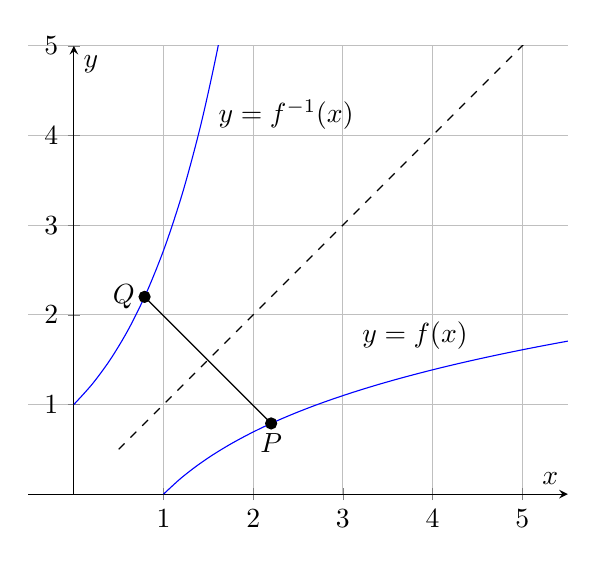
\begin{tikzpicture}
		\begin{axis}[
			xmin=0,xmax=5,
			ymin=0,ymax=5,
			restrict y to domain=0:10,
			grid=both,
			axis equal=true,
			axis lines=middle,
			xlabel=$x$,
			ylabel=$y$,
			axis lines=middle,
		]
			\begin{scope}[color=blue,samples=50,smooth]
				\addplot[domain=0:10]{exp(x)};
				\addplot[domain=1:10]{ln(x)};
			\end{scope}
			\addplot[color=black,dashed,domain=.5:8]{x};
			\filldraw(2.2,{ln(2.2)})circle(2pt)node[below]{$P$}
				--({ln(2.2)},2.2)circle(2pt)node[left]{$Q$};
			\draw(4.5,{ln(4.5)})node[above left]{$y=f(x)$}
				({ln(4.5)},4.5)node[below right]{$y=f^{-1}(x)$};
		\end{axis}
	\end{tikzpicture}
	\caption{}\label{figure:函数.直接函数与反函数的图形的对称性}
\end{figure}

\subsection{复合函数}
\begin{definition}
设函数\(y=f(u)\)的定义域为\(D_f\),
函数\(u=g(x)\)的定义域为\(D_g\),
且其值域\(R_g \subseteq D_f\),
则函数\[
	y = f[g(x)],
	\quad x \in D_g
\]
称为由函数\(u=g(x)\)与函数\(y=f(u)\)构成的\DefineConcept{复合函数},
它的定义域为\(D_g\),变量\(u\)称为\DefineConcept{中间变量}.

函数\(g\)与函数\(f\)构成的复合函数,
即按“先\(g\)后\(f\)”的次序复合的函数,
通常记为\(f \circ g\),即\[
	(f \circ g)(x) = f[g(x)].
\]
\end{definition}

\begin{proposition}
设\(f\)和\(g\)都是奇函数,
则\(f \circ g\)也是奇函数.
\begin{proof}
这是因为\(f[g(-x)]
= f[-g(x)]
= -f[g(x)]\).
\end{proof}
\end{proposition}

\begin{proposition}
设\(f\)和\(g\)都是偶函数,
则\(f \circ g\)也是偶函数.
\begin{proof}
这是因为\(f[g(-x)]
= f[g(x)]\).
\end{proof}
\end{proposition}

\begin{proposition}
设\(f\)是奇函数,\(g\)是偶函数,
则\(f \circ g\)和\(g \circ f\)都是偶函数.
\begin{proof}
这是因为\(f[g(-x)]
= f[g(x)]\),
\(g[f(-x)]
= g[-f(x)]
= g[f(x)]\).
\end{proof}
\end{proposition}

\begin{proposition}
设\(f\)和\(g\)是严格单调增加函数,
则\(f \circ g\)是严格单调增加函数.
\begin{proof}
对于\(\forall x_1,x_2 \in \dom(f \circ g)\),
当\(x_1 < x_2\)时,
有\(g(x_1) < g(x_2)\),
从而有\(f[g(x_1)] < f[g(x_2)]\),
这就说明\(f \circ g\)是严格单调增加函数.
\end{proof}
\end{proposition}

\begin{proposition}
设\(f\)和\(g\)是严格单调减少函数,
则\(f \circ g\)是严格单调增加函数.
\begin{proof}
对于\(\forall x_1,x_2 \in \dom(f \circ g)\),
当\(x_1 < x_2\)时,
有\(g(x_1) > g(x_2)\),
从而有\(f[g(x_1)] < f[g(x_2)]\),
这就说明\(f \circ g\)是严格单调增加函数.
\end{proof}
\end{proposition}

\begin{proposition}
设\(f\)是严格单调增加函数,
\(g\)是严格单调减少函数,
则\(f \circ g\)和\(g \circ f\)都是严格单调减少函数.
\begin{proof}
对于\(\forall x_1,x_2 \in \dom(f \circ g)\),
当\(x_1 < x_2\)时,
有\(g(x_1) > g(x_2)\),
从而有\(f[g(x_1)] > f[g(x_2)]\),
这就说明\(f \circ g\)是严格单调减少函数.
同理可证\(g \circ f\)也是严格单调减少函数.
\end{proof}
\end{proposition}

\section{绝对值函数}
\begin{definition}[绝对值]
设\(x \in \mathbb{R}\),则称函数\[
	f(x) = \left\{ \begin{array}{c}
		x, \quad x \geq 0 \\
		-x, \quad x < 0
	\end{array} \right.
\]为\(x\)的绝对值,
记作\(\abs{x}\).
\end{definition}

\begin{figure}[ht]
	\centering
	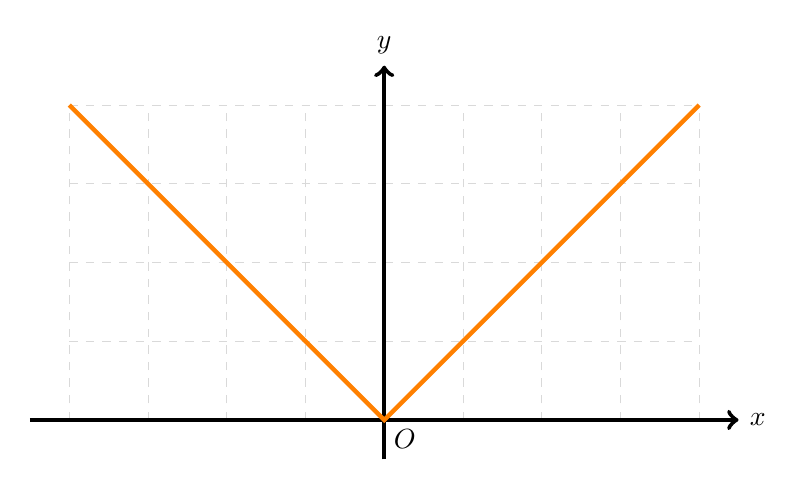
\begin{tikzpicture}
		\draw[help lines, color=gray!30, dashed] (-4,0) grid (4,4);
		\draw[->, ultra thick] (-4.5,0) -- (4.5,0) node[right]{\(x\)};
		\draw[->, ultra thick] (0,-0.5) -- (0,4.5) node[above]{\(y\)};
		\draw (0,0)node[below right]{\(O\)};
		\draw[orange,ultra thick] (-4,4)--(0,0)--(4,4);
	\end{tikzpicture}
	\caption{绝对值函数\(\abs{x}\)的图形}
\end{figure}

\begin{proposition}
设\(a,b\in\mathbb{R}\),
则\(\abs{ab} = \abs{a} \abs{b}\).
\begin{proof}
当\(a=0\)或\(b=0\)时,易见\(\abs{ab} = 0 = \abs{a} \abs{b}\).
当\(a\neq0\)且\(b\neq0\)时,
按照\(a\)和\(b\)的不同取值,列表如下:
\begin{center}
	\begin{tblr}{|*2c|*2{c|}}
		\hline
		&& \(b>0\) & \(b<0\) \\
		&& \(\abs{b}=b\) & \(\abs{b}=-b\) \\ \hline
		\(a>0\) & \(\abs{a}=a\) & \(ab>0,\abs{ab}=ab\) & \(ab<0,\abs{ab}=-ab\) \\ \hline
		\(a<0\) & \(\abs{a}=-a\) & \(ab<0,\abs{ab}=-ab\) & \(ab>0,\abs{ab}=ab\) \\ \hline
	\end{tblr}
\end{center}
由此可知\(\abs{ab} = \abs{a} \abs{b}\)恒成立.
\end{proof}
\end{proposition}

\begin{proposition}
设\(a\)和\(b\)都是实数,
则\begin{gather}
	\min\{a,b\}
	= \frac{a+b}{2}
	- \frac{\abs{a-b}}{2}, \\
	\max\{a,b\}
	= \frac{a+b}{2}
	+ \frac{\abs{a-b}}{2}.
\end{gather}
\begin{proof}
当\(a>b\)时,有\[
	\frac{a+b}{2} - \frac{\abs{a-b}}{2}
	= \frac{a+b}{2} - \frac{a-b}{2}
	= \frac{2b}{2} = b
	= \min\{a,b\},
\]\[
	\frac{a+b}{2} + \frac{\abs{a-b}}{2}
	= \frac{a+b}{2} + \frac{a-b}{2}
	= \frac{2a}{2} = a
	= \max\{a,b\}.
\]
当\(a \leq b\)时,有\[
	\frac{a+b}{2} - \frac{\abs{a-b}}{2}
	= \frac{a+b}{2} - \frac{b-a}{2}
	= \frac{2a}{2} = a
	= \min\{a,b\},
\]\[
	\frac{a+b}{2} + \frac{\abs{a-b}}{2}
	= \frac{a+b}{2} + \frac{b-a}{2}
	= \frac{2b}{2} = b
	= \max\{a,b\}.
	\qedhere
\]
\end{proof}
\end{proposition}

\section{符号函数}
\begin{definition}[符号函数]
函数\[
	f(x) = \left\{ \begin{array}{cc}
		1, & x > 0 \\
		0, & x = 0 \\
		-1, & x < 0 \\
	\end{array} \right.
\]称为\DefineConcept{符号函数},
记作\(\sgn x\).
\end{definition}

\begin{figure}[htb]
	\centering
	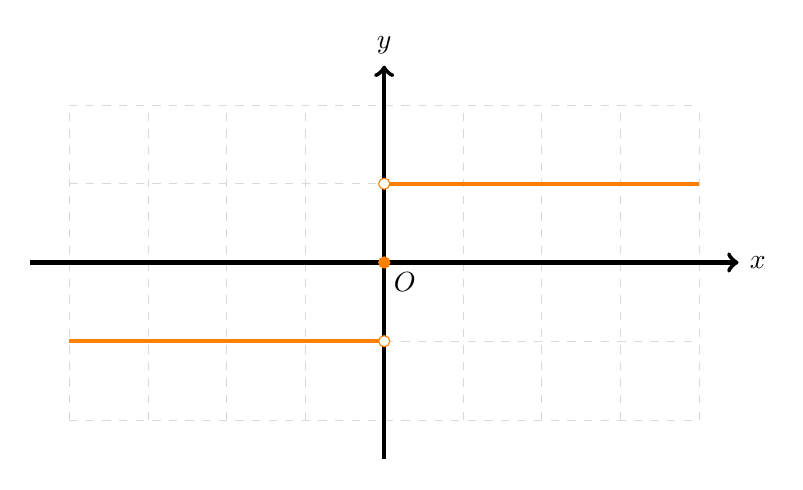
\begin{tikzpicture}
		\draw[help lines, color=gray!30, dashed] (-4,-2) grid (4,2);
		\draw[->, ultra thick] (-4.5,0) -- (4.5,0) node[right]{\(x\)};
		\draw[->, ultra thick] (0,-2.5) -- (0,2.5) node[above]{\(y\)};
		\draw (0,0)node[below right]{\(O\)};
		\draw[orange,ultra thick] (-4,-1)--(0,-1) (0,1)--(4,1);
		\draw[draw=orange,fill=orange] (0,0)circle(2pt);
		\draw[draw=orange,fill=white] (0,1)circle(2pt) (0,-1)circle(2pt);
	\end{tikzpicture}
	\caption{符号函数\(\sgn x\)的图形}
\end{figure}

\section{取整函数}
\begin{definition}[取整函数]
设\(x\in\mathbb{R},
n\in\mathbb{Z}\),定义:
\begin{enumerate}
	\item 如果\(n\)是不大于\(x\)的最大整数,
	即\(x\in[n,n+1)\),
	那么记\(\floor{x}=n\).
	我们把函数\(y=\floor{x}\)称为\DefineConcept{向下取整函数},
	即\begin{equation}
		\floor{x}
		\defeq
		\max\Set{ n\in\mathbb{Z} \given n \leq x }.
	\end{equation}

	\item 如果\(n\)是不小于\(x\)的最小整数,
	即\(x\in(n-1,n]\),
	那么记\(\ceil{x}=n\).
	我们把函数\(y=\ceil{x}\)称为\DefineConcept{向上取整函数},
	即\begin{equation}
		\ceil{x}
		\defeq
		\min\Set{ n\in\mathbb{Z} \given n \geq x }.
	\end{equation}
\end{enumerate}
\end{definition}

\begin{figure}[ht]
	\def\subwidth{.45\linewidth}
	\def\subscale{.9}
	\begin{subfigure}[b]{\subwidth}%
		\centering
		\begin{tikzpicture}[scale=\subscale]
			\tikzstyle{sx}=[draw=orange,fill=orange]
			\tikzstyle{kx}=[draw=orange,fill=white]
			\draw[help lines, color=gray!30, dashed] (-1,-1) grid (4,4);
			\draw[dashed, color=gray] (-1,-1) -- (4,4);
			\draw[->, thick] (-1.5,0) -- (4.5,0) node[right]{\(x\)};
			\draw[->, thick] (0,-1.5) -- (0,4.5) node[above]{\(y\)};
			\foreach \i in {-1,...,3} {
				\draw[ultra thick,orange] (\i,\i)--(\i+1,\i);
				\fill[sx] (\i,\i)circle(2pt);
				\fill[kx] (\i+1,\i)circle(2pt);
				\ifnum\i=0\relax\else
					\draw(\i,0)node[below right]{\i};
					\draw(0,\i)node[above right]{\i};
				\fi
			}
			\draw (0,0)node[above left]{\(O\)};
		\end{tikzpicture}
		\subcaption{向下取整函数\(\floor{x}\)}
	\end{subfigure}
	\begin{subfigure}[b]{\subwidth}%
		\centering
		\begin{tikzpicture}[scale=\subscale]
			\tikzstyle{sx}=[draw=orange,fill=orange]
			\tikzstyle{kx}=[draw=orange,fill=white]
			\draw[help lines, color=gray!30, dashed] (-1,-1) grid (4,4);
			\draw[dashed, color=gray] (-1,-1) -- (4,4);
			\draw[->, thick] (-1.5,0) -- (4.5,0) node[right]{\(x\)};
			\draw[->, thick] (0,-1.5) -- (0,4.5) node[above]{\(y\)};
			\foreach \i in {-1,...,3} {
				\draw[ultra thick,orange] (\i,\i+1)--(\i+1,\i+1);
				\fill[kx] (\i,\i+1)circle(2pt);
				\fill[sx] (\i+1,\i+1)circle(2pt);
				\ifnum\i=0\relax\else
					\draw(\i,0)node[below right]{\i};
					\draw(0,\i)node[above right]{\i};
				\fi
			}
			\draw (0,0)node[above left]{\(O\)};
		\end{tikzpicture}
		\subcaption{向上取整函数\(\ceil{x}\)}
	\end{subfigure}
	\caption{取整函数的图形}
\end{figure}

\begin{property}\label{theorem:取整函数.性质1}
一般地,对于\(x\in\mathbb{R}\),总有\begin{equation}
	x - 1 < \floor{x} \leq x \leq \ceil{x} < x + 1.
\end{equation}
\end{property}

\begin{property}
对于\(n\in\mathbb{Z}\),总有\begin{equation}
	\ceil{n/2} + \floor{n/2} = n.
\end{equation}
\end{property}

\begin{property}
对于任意实数\(x \geq 0\)和整数\(a,b>0\),总有\begin{gather}
	\ceil*{\frac{\ceil{x/a}}{b}} = \ceil*{\frac{x}{ab}}, \\
	\floor*{\frac{\floor{x/a}}{b}} = \floor*{\frac{x}{ab}}, \\
	\ceil*{\frac{a}{b}} \leq \frac{a+(b-1)}{b}, \\
	\floor*{\frac{a}{b}} \geq \frac{a-(b-1)}{b}.
\end{gather}
\end{property}

\section{幂函数、指数函数、对数函数}
\begin{definition}
同一个数\(a\ (a\in\mathbb{R})\)连续相乘\(b\ (b\in\mathbb{N})\)次所得的乘积,
称作“\(a\)的\(b\)次方”
或“\(a\)的\(b\)次幂”,
记作\(a^b\),
即\[
	a^b
	\defeq
	\underbrace{a \times a \times \dotsm \times a}_{b\text{次}} = \prod_{i=1}^b a.
\]

特别地,规定:\begin{gather*}
	a^0 \defeq 1 \quad(a\neq0), \\
	a^{-1} \defeq \frac1a \quad(a\neq0), \\
	a^{-n} \defeq \frac1{a^n} \quad(a\neq0), \\
	a^{1/n} \defeq \sqrt[n]{a} \quad(a\geq0). \\
\end{gather*}
\end{definition}

\begin{figure}[ht]
	\centering
	\begin{tikzpicture}
		\def\r{\textcolor{orange}}
		\def\b{\textcolor{blue}}
		\def\p{\textcolor{purple}}
		\draw(0,0)node{\(\r{a}^{\b{b}} = \p{c} \defiff \log_{\r{a}} \p{c} = \b{b}\)};
		\draw(-2.2,-.5)node{\r{底数}}
			(-2.2,.5)node{\b{指数}}
			(-1,-.5)node{\p{幂}}
			(.3,-.5)node{\r{底数}}
			(1.4,-.5)node{\p{真数}}
			(2.3,.5)node{\b{对数}};
		\draw[->](-1.7,-.3)--(-1.7,-1)--(.84,-1)->(.84,-.3); %a
		\draw[->](-1.55,.3)--(-1.55,1)--(1.7,1)->(1.7,.3); %b
		\draw[->](-.86,.3)--(-.86,.7)--(1.1,.7)->(1.1,.3); %c
	\end{tikzpicture}
	\caption{底数、指数、幂与对数的联系}\label{figure:函数.底数、指数、幂与对数的联系}
\end{figure}

\begin{proposition}
\(1\)的任意次幂还是\(1\),即\(1^n = 1\).
\end{proposition}

\begin{proposition}
\(0\)的任意非零次幂还是\(0\),即\(0^n = 0\ (n\neq0)\).
\end{proposition}

\subsection{幂函数的概念}
\begin{definition}[幂函数]
函数\(f(x)=x^{\mu}\ (\mu \in \mathbb{R})\),
称为\DefineConcept{幂函数}.
\end{definition}

\subsection{幂函数的性质}
\begin{property}
幂函数具有以下性质:
\begin{itemize}
	\item 当\(\mu = 0\)时,
	幂函数\(f(x)=x^{\mu}\)在定义域\((-\infty,+\infty)\)上恒为一,
	是常数函数.

	\item 当\(\mu\)为正奇数时,
	幂函数\(f(x)=x^{\mu}\)为奇函数,
	其定义域、值域均为\((-\infty,+\infty)\),它在定义域内恒单调递增.

	\item 当\(\mu\)为正偶数时,
	幂函数\(f(x)=x^{\mu}\)为偶函数,
	其定义域为\((-\infty,+\infty)\),其值域为\([0,+\infty)\),
	它在\((-\infty,0]\)上单调递减,在\([0,+\infty)\)上单调递增.

	\item 当\(\mu\)为负奇数时,
	幂级数\(y=x^{\mu}\)又称为\DefineConcept{比例函数},
	其定义域、值域为\((-\infty,0)\cup(0,+\infty)\),
	它在区间\((-\infty,0)\)和\((0,+\infty)\)内单调递减.

	若幂函数前有常系数大于零则称之为\DefineConcept{正比例函数}.
	%@Mathematica: Plot[Evaluate[x^-n /. n -> {1, 2, 3, 4, 5}], {x, 0, 2}, PlotRange -> {0, 2}, PlotLegends -> Automatic]

	若幂函数前有常系数小于零则称之为\DefineConcept{反比例函数}.
	%@Mathematica: Plot[Evaluate[x^-n /. n -> {1, 2, 3, 4, 5}], {x, -2, 0}, PlotRange -> {-2, 2}, PlotLegends -> Automatic]

	\item 当\(\mu\)为负偶数时,
	幂函数\(f(x)=x^{\mu}\)为偶函数,
	其定义域为\((-\infty,0)\cup(0,+\infty)\),其值域为\((0,+\infty)\),
	它在\((-\infty,0)\)内单调递增,在\((0,+\infty)\)内单调递减.

	\item 当\(\mu = \pm\frac{m}{n} \in \mathbb{Q}\)(\(m,n>0\)且\(m\)、\(n\)是互质的整数)时,
	幂函数\(f(x)=x^{\mu}=x^{\pm\frac{m}{n}}\)可改写为\(y=\sqrt[n]{x^m}\)(\(\mu>0\)时)
	或\(y=\frac{1}{\sqrt[n]{x^m}}\)(\(\mu<0\)时).
\end{itemize}
\end{property}

\begin{figure}[ht]
	\centering
	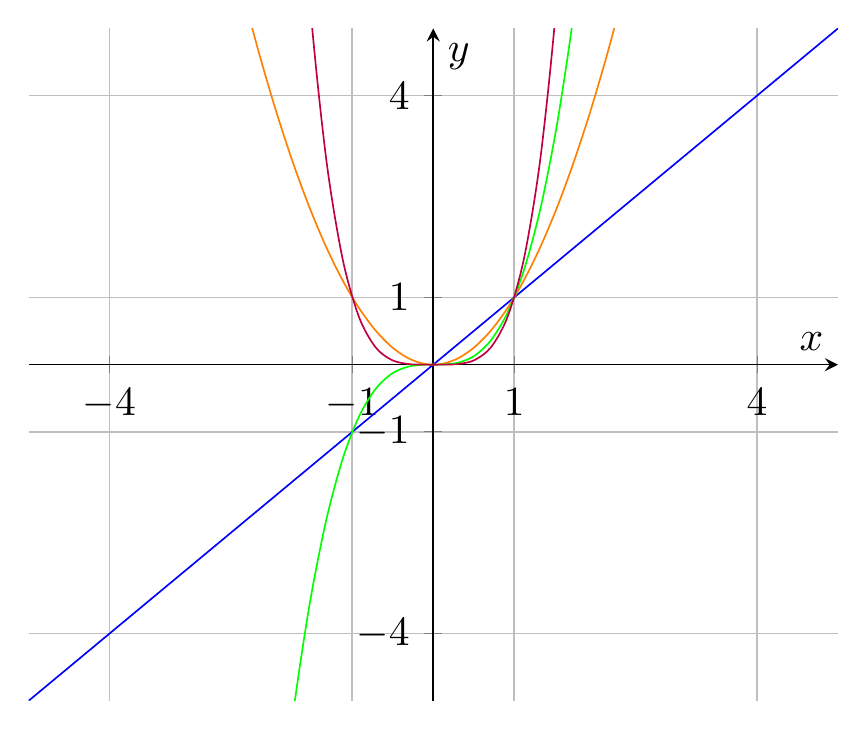
\begin{tikzpicture}[scale=1.5]
		\begin{axis}[
			xmin=-5,xmax=5,
			ymin=-5,ymax=5,
			enlargelimits,
			axis lines=middle,
			xlabel=$x$,
			ylabel=$y$,
			xtick={-4,-1,1,4},
			ytick={-4,-1,1,4},
			grid=major,
		]
			\begin{scope}[samples=50,smooth,domain=-5:5]
				\addplot[color=blue]{x};
				\addplot[color=orange]{x^2};
				\addplot[color=green]{x^3};
				\addplot[color=purple]{x^4};
			\end{scope}
		\end{axis}
	\end{tikzpicture}
	\caption{}
\end{figure}

\begin{figure}
	\centering
	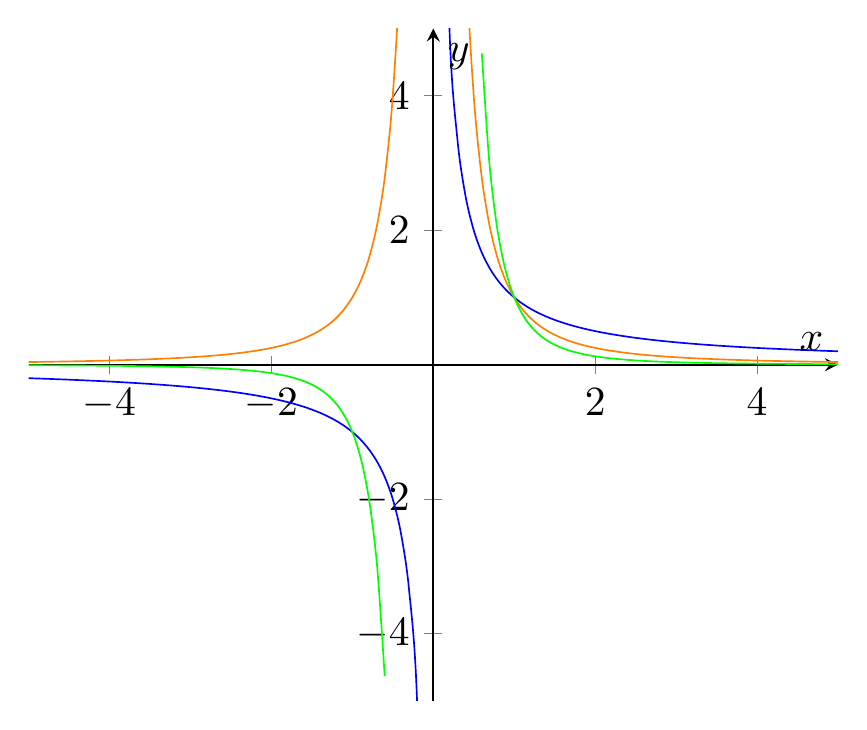
\begin{tikzpicture}[scale=1.5]
		\begin{axis}[
			xmin=-5,xmax=5,
			ymin=-5,ymax=5,
			enlargelimits,
			axis lines=middle,
			xlabel=$x$,
			ylabel=$y$,
		]
			\begin{scope}[samples=50,smooth]
				\begin{scope}[domain=-5:-.1]
					\addplot[color=blue]{1/x};
					\addplot[color=orange]{1/(x^2)};
					\addplot[color=green,domain=-5:-.6]{1/(x^3)};
				\end{scope}
				\begin{scope}[domain=.1:5]
					\addplot[color=blue]{1/x};
					\addplot[color=orange]{1/(x^2)};
					\addplot[color=green,domain=.6:5]{1/(x^3)};
				\end{scope}
			\end{scope}
		\end{axis}
	\end{tikzpicture}
	\caption{}
\end{figure}

\subsection{指数函数的概念}
\begin{definition}
设\(a>0\)且\(a \neq 1\).
把函数\(f(x)=a^x\)
称为“以\(a\)为底的\DefineConcept{指数函数}”.
\end{definition}

\begin{theorem}
设\(f\)是以\(a\)为底的指数函数,
则\(f\)存在反函数.
\begin{proof}
指数函数是单调函数.
\end{proof}
\end{theorem}

\subsection{指数函数的性质}
\begin{property}
\begin{gather}
	a^x a^y = a^{x+y}, \\
	\frac{a^x}{a^y} = a^{x-y}, \\
	(a^x)^y = a^{xy}.
\end{gather}
\end{property}

\subsection{对数函数的概念}
\begin{definition}
设\(a>0\)且\(a\neq1\).
以\(a\)为底的指数函数的反函数,
称为“以\(a\)为底的\DefineConcept{对数函数}”,
记作\(\log_a x\),
即\begin{equation}\label{equation:函数.对数的定义}
	y = \log_a x
	\defiff
	a^y = x.
\end{equation}
%@see: https://mathworld.wolfram.com/Logarithm.html
\end{definition}

以\(10\)为底的对数,称为\DefineConcept{常用对数},记作\(y = \lg x\),
即\begin{equation}
	\lg x \defeq \log_{10} x.
\end{equation}

以常数\(e\)为底的对数,称为\DefineConcept{自然对数},记作\(y = \ln x\),
即\begin{equation}
	\ln x \defeq \log_e x.
\end{equation}

\subsection{对数函数的性质}
\begin{proposition}[对数恒等式]
设\(a>0,a\neq1\),
则对\(\forall x>0\)
有\begin{equation}\label{equation:函数.对数恒等式}
	a^{\log_a x} = x.
\end{equation}
\begin{proof}
根据\hyperref[equation:函数.对数的定义]{对数的定义}有
\(y = \log_a x
\defiff
a^y = x\),
于是\(a^{\log_a x} = a^y = x\).
\end{proof}
\end{proposition}

\begin{theorem}
设\(a>0,a\neq1\),
则\begin{gather}
	\log_a 1 = 0, \\
	\log_a a = 1.
\end{gather}
\end{theorem}

\begin{theorem}[对数的运算法则]
设\(a>0,a\neq1,x>0,y>0\),
则\begin{gather}
	\log_a xy = \log_a x + \log_a y,
		\label{equation:函数.对数的基本运算法则1} \\
	\log_a \frac{x}{y} = \log_a x - \log_a y,
		\label{equation:函数.对数的基本运算法则2} \\
	\log_a x^y = y \log_a x.
		\label{equation:函数.对数的基本运算法则3}
\end{gather}
\end{theorem}

\begin{theorem}[换底公式]
设\(a>0,a\neq1,c>0,c\neq1,b>0\),
则\begin{equation}\label{equation:函数.换底公式}
	\log_a b = \frac{\log_c b}{\log_c a}.
\end{equation}
\begin{proof}
由\hyperref[equation:函数.对数恒等式]{对数恒等式}有\(b = a^{\log_a b}\),
于是\(\log_c b
= \log_c a^{\log_a b}\).
又由有\hyperref[equation:函数.对数的基本运算法则3]{对数的运算法则}有\[
	\log_c a^{\log_a b} = \log_a b \cdot \log_c a,
\]
所以\(\log_a b = \frac{\log_c b}{\log_c a}\).
\end{proof}
\end{theorem}

\begin{corollary}
设\(a>0,a\neq1,b>0,b\neq1\),
则\begin{equation}
	\log_a b = \frac1{\log_b a}.
\end{equation}
\begin{proof}
在\hyperref[equation:函数.换底公式]{换底公式}中,令\(c=b\)便得.
\end{proof}
\end{corollary}

\begin{corollary}
设\(a>0,a\neq1,a^x\neq1\)
则\begin{equation}
	\log_{a^x} b^y = \frac{y}{x} \log_a b.
\end{equation}
\end{corollary}

\begin{example}
设\(a>0,b>0\).
证明:\begin{equation}\label{equation:函数.真底互换公式}
	a^{\ln b} = b^{\ln a}.
\end{equation}
\begin{proof}
在\cref{equation:函数.真底互换公式} 等号左右变量分别取对数,
得\[
	\ln(a^{\ln b}) = \ln b \ln a, \qquad
	\ln(b^{\ln a}) = \ln a \ln b,
\]
显然两者相等,故\(a^{\ln b} = b^{\ln a}\)成立.
\end{proof}
\end{example}

\subsection{重幂}
设\(a\)是实数,\(b\)是正整数.
定义:\[
	\relax^ba \defeq \underbrace{a^{a^{\iddots^a}}}_{\text{\(b\)个}},
\]
我们把\(\relax^ba\)读作“\(a\)的\(b\)~\DefineConcept{重幂}”.

例如,\[
	\relax^23 = 3^3, \qquad
	\relax^33 = 3^{3^3}, \qquad
	\relax^43 = 3^{3^{3^3}}.
\]

\section{三角函数}
\subsection{三角函数的概念}
\begin{figure}[htb]
	\centering
	\begin{tikzpicture}[scale=6]
		\draw(1,0)coordinate(A)node[below]{$A$}
			arc[start angle=0,end angle=90,radius=1](0,1)node[left]{$B$};
		\draw(0,0)coordinate(O)node[below left]{$O$}
			--(.866,.5)coordinate(P)node[above]{$P$}
			--(.866,0)coordinate(Q)node[below]{$Q$};
		\draw(P)--(1,.577)coordinate(R)node[right]{$R$}--(A);
		\begin{scope}[->,>=Stealth]
			\draw(0,0)--(1.2,0)node[below]{$x$};
			\draw(0,0)--(0,1.2)node[left]{$y$};
		\end{scope}
		\draw pic["$\theta$",draw=orange,-,angle eccentricity=1.2,angle radius=1cm]{angle=Q--O--P};
		\draw pic[draw=gray,-,angle radius=.5cm]{right angle=P--Q--O};
	\end{tikzpicture}
	\caption{}
	\label{figure:函数.三角函数.三角函数的几何定义}
\end{figure}

如\cref{figure:函数.三角函数.三角函数的几何定义},
首先在平面直角坐标系\(Oxy\)中
画出一个单位圆\(\odot~O\),
分别交\(x\)轴、\(y\)轴于\(A\)、\(B\)两点.
在\(\odot~O\)上任取一点\(P\),过\(P\)作\(OA\)的垂线交\(OA\)于\(Q\).
过点\(A\)作\(OA\)的垂线交射线\(OP\)于\(R\).
记\(\angle POQ = \theta\).
定义:\begin{gather}
	\sin\theta \defeq \abs{\overline{PQ}}, \\
	\cos\theta \defeq \abs{\overline{OQ}}, \\
	\tan\theta \defeq \sin\theta/\cos\theta, \\
	\cot\theta \defeq \cos\theta/\sin\theta, \\
	\sec\theta \defeq 1/\cos\theta, \\
	\csc\theta \defeq 1/\sin\theta.
\end{gather}
我们把\(\sin,\cos,\tan,\cot,\sec,\csc\)
依次称为\DefineConcept{正弦函数}、
\DefineConcept{余弦函数}、
\DefineConcept{正切函数}、
\DefineConcept{余切函数}、
\DefineConcept{正割函数}、
\DefineConcept{余割函数},
统称为\DefineConcept{三角函数}.

不难想象,当\(P\)在圆周上逆时针平移时,
\(\theta\)逐渐增大,
线段\(\overline{OP}\)的长度\(\abs{\overline{OP}}\)始终保持不变,
线段\(\overline{PQ}\)的长度\(\abs{\overline{PQ}}\)逐渐增大,
线段\(\overline{OQ}\)的长度\(\abs{\overline{OQ}}\)逐渐减小.
当\(P\)与\(B\)重合时,
\(\abs{\overline{OP}}
= \abs{\overline{PQ}}
= \abs{\overline{OB}} = 1\)
且\(\abs{\overline{OQ}} = 0\).
当\(P\)在圆周上顺时针平移时,
\(\theta\)逐渐减小,
线段\(\overline{OP}\)的长度\(\abs{\overline{OP}}\)依旧始终保持不变,
线段\(\overline{PQ}\)的长度\(\abs{\overline{PQ}}\)逐渐减小,
线段\(\overline{OQ}\)的长度\(\abs{\overline{OQ}}\)逐渐增大.
当\(P\)与\(A\)重合时,
\(\abs{\overline{OP}}
= \abs{\overline{OA}} = 1\)
且\(\abs{\overline{PQ}} = 0\).

\begin{example}
下面列出一些特殊的正弦函数值:\[
	\sin0 = 0, \quad
	\sin\frac{\pi}{6} = \frac{1}{2}, \quad
	\sin\frac{\pi}{4} = \frac{\sqrt{2}}{2}, \quad
	\sin\frac{\pi}{3} = \frac{\sqrt{3}}{2},
\]\[
	\sin\frac{\pi}{2} = 1, \quad
	\sin\pi = 0, \quad
	\sin\frac{3\pi}{2} = -1.
\]

\begin{figure}[htb]
	\centering
	\begin{tikzpicture}
		\pgfmathsetmacro{\r}{2}
		\pgfmathsetmacro{\ax}{\r*cos(30)}
		\pgfmathsetmacro{\ay}{\r*sin(30)}
		\pgfmathsetmacro{\b}{\r/sqrt(2)}
		\coordinate (O)at(0,0);
		\draw(O)circle(\r);
		\begin{scope}[dashed,color=gray!50,text=black]
			\draw(O)--(\r,0)node[left]{\(0\)}node[right]{\(0\)}
			(O)--(\ax,\ay)node[below left]{\(\tfrac{\pi}{6}\)}node[right]{\(\tfrac{1}{2}\)}
			(O)--(\b,\b)node[below left]{\(\tfrac{\pi}{4}\)}node[above right]{\(\tfrac{\sqrt2}{2}\)}
			(O)--(\ay,\ax)node[below left]{\(\tfrac{\pi}{3}\)}node[above]{\(\tfrac{\sqrt3}{2}\)}
			(O)--(0,\r)node[below]{\(\tfrac{\pi}{2}\)}node[above]{\(1\)}
			(O)--(-\ay,\ax)node[below right]{\(\tfrac{2\pi}{3}\)}node[above]{\(\tfrac{\sqrt3}{2}\)}
			(O)--(-\b,\b)node[below right]{\(\tfrac{3\pi}{4}\)}node[above left]{\(\tfrac{\sqrt2}{2}\)}
			(O)--(-\ax,\ay)node[below right]{\(\tfrac{5\pi}{6}\)}node[left]{\(\tfrac{1}{2}\)}
			(O)--(-\r,0)node[right]{\(\pi\)}node[left]{\(0\)}
			(O)--(-\ax,-\ay)node[above right]{\(\tfrac{7\pi}{6}\)}node[left]{\(-\tfrac{1}{2}\)}
			(O)--(-\b,-\b)node[above right]{\(\tfrac{5\pi}{4}\)}node[below left]{\(-\tfrac{\sqrt2}{2}\)}
			(O)--(-\ay,-\ax)node[above right]{\(\tfrac{4\pi}{3}\)}node[below]{\(-\tfrac{\sqrt3}{2}\)}
			(O)--(0,-\r)node[above]{\(\tfrac{3\pi}{2}\)}node[below]{\(-1\)}
			(O)--(\ay,-\ax)node[above left]{\(\tfrac{5\pi}{3}\)}node[below]{\(-\tfrac{\sqrt3}{2}\)}
			(O)--(\b,-\b)node[above left]{\(\tfrac{7\pi}{4}\)}node[below right]{\(-\tfrac{\sqrt2}{2}\)}
			(O)--(\ax,-\ay)node[above left]{\(\tfrac{11\pi}{6}\)}node[right]{\(-\tfrac{1}{2}\)}
			;
		\end{scope}
		\begin{scope}[very thick,->]
			\draw(-1,0)--(1,0)node[above left]{\(x\)};
			\draw(0,-1)--(0,1)node[below right]{\(y\)};
		\end{scope}
	\end{tikzpicture}
	\caption{正弦函数\(\sin x\)的辅助圆与特殊值}
\end{figure}

特殊的余弦函数值:\[
	\cos0 = 1, \quad
	\cos\frac{\pi}{6} = \frac{\sqrt{3}}{2}, \quad
	\cos\frac{\pi}{4} = \frac{\sqrt{2}}{2}, \quad
	\cos\frac{\pi}{3} = \frac{1}{2},
\]\[
	\cos\frac{\pi}{2} = 0, \quad
	\cos\pi = -1, \quad
	\cos\frac{3\pi}{2} = 0.
\]
\end{example}

\subsection{三角函数的性质}
\begin{property}
根据三角函数的定义,显然有\begin{gather}
	\tan\theta = \frac{\sin\theta}{\cos\theta},
	\label{equation:三角函数.正切与正余弦的关系} \\
	\cot\theta = \frac{1}{\tan\theta}, \\
	\sec\theta = \frac{1}{\cos\theta}, \\
	\csc\theta = \frac{1}{\sin\theta}.
\end{gather}
\end{property}

\begin{theorem}[毕达哥拉斯三角恒等式]
\begin{figure}[htb]
	\def\subwidth{.5\linewidth}
	\def\subscale{.8}
		\begin{subfigure}[b]{\subwidth}%
		\centering
		\begin{tikzpicture}[scale=\subscale]
			\draw[help lines, color=gray!30, dashed] (0,0) grid (4,3);
			\coordinate (A) at (0,0);
			\coordinate (B) at (4,0);
			\coordinate (C) at (4,3);
			\draw (A)node[left]{\(A\)} -- (B)node[right]{\(B\)}node[midway,below]{\(\cos\theta\)} -- (C)node[right]{\(C\)}node[midway,right]{\(\sin\theta\)} -- (A)node[midway,above left]{\(1\)} pic["\(\theta\)",draw=orange,-,angle eccentricity=2,angle radius=0.3cm]{angle=B--A--C} pic[draw=gray,-,angle radius=0.3cm]{right angle=C--B--A};
		\end{tikzpicture}
		\subcaption{正弦、余弦辅助三角形}
		\end{subfigure}%
		\begin{subfigure}[b]{\subwidth}%
		\centering
		\begin{tikzpicture}[scale=\subscale]
			\draw[help lines, color=gray!30, dashed] (0,0) grid (4,3);
			\coordinate (A) at (0,0);
			\coordinate (B) at (4,0);
			\coordinate (C) at (4,3);
			\draw (A)node[left]{\(A\)} -- (B)node[right]{\(B\)}node[midway,below]{\(1\)} -- (C)node[right]{\(C\)}node[midway,right]{\(\tan\theta\)} -- (A)node[midway,above left]{\(\sec\theta\)} pic["\(\theta\)",draw=orange,-,angle eccentricity=2,angle radius=0.3cm]{angle=B--A--C} pic[draw=gray,-,angle radius=0.3cm]{right angle=C--B--A};
		\end{tikzpicture}
		\subcaption{正切、正割辅助三角形}
		\end{subfigure}%
	\caption{两种特殊的辅助三角形}
	\label{figure:函数.两种特殊的辅助三角形}
\end{figure}

结合\cref{figure:函数.两种特殊的辅助三角形},根据勾股定理可得
\begin{gather}
	\sin^2 \theta + \cos^2 \theta = 1,
		\label{equation:三角函数.毕达哥拉斯三角恒等式1} \\
	\tan^2 \theta + 1 = \sec^2 \theta, \\
	1 + \cot^2 \theta = \csc^2 \theta.
\end{gather}
\end{theorem}

\begin{figure}[htb]
	\centering
	\begin{tikzpicture}
		\pgfmathsetmacro{\a}{6}
		\coordinate(O)at(0,0);
		\pgfmathsetmacro{\t}{30}
		\draw(O)node[below left]{\(O\)}
			--(\a,0)coordinate(A)node[below right]{\(A\)}
			arc[start angle=0,end angle=\t,radius=\a]coordinate(B)node[right]{\(B\)}
			--(O);
		\draw(B)--(B|-A)coordinate(C)node[below right]{\(C\)};
		\draw(B)--(\a,{\a*tan(\t)})coordinate(D)node[above right]{\(D\)}--(\a,0);
		\pic["\(\theta\)",draw,-,angle eccentricity=1.5,angle radius=6mm]{angle=A--O--B};
		\begin{scope}[|<->|,black!40,every node/.style={black,midway,sloped}]
			\def\mark#1#2#3#4#5{%
				\draw($#1+#4$)--($#2+#4$)node[#3]{$#5$};%
			}%
			\mark{(C)}{(B)}{above}{(-5pt,0)}{\sin\theta}
			\mark{(O)}{(D)}{above}{({(-1em-10pt)*sin(30)},{(1em+10pt)*cos(30)})}{\sec\theta}
			\mark{(O)}{(B)}{above}{({-5pt*sin(30)},{5pt*cos(30)})}{1}
			\mark{(O)}{(C)}{below}{(0,-5pt)}{\cos\theta}
			\mark{(A)}{(D)}{below}{(5pt,0)}{\tan\theta}
			\mark{(O)}{(A)}{below}{(0,-1em-10pt)}{1}
		\end{scope}
	\end{tikzpicture}
	\caption{}
\end{figure}

\begin{figure}[htb]
	\centering
	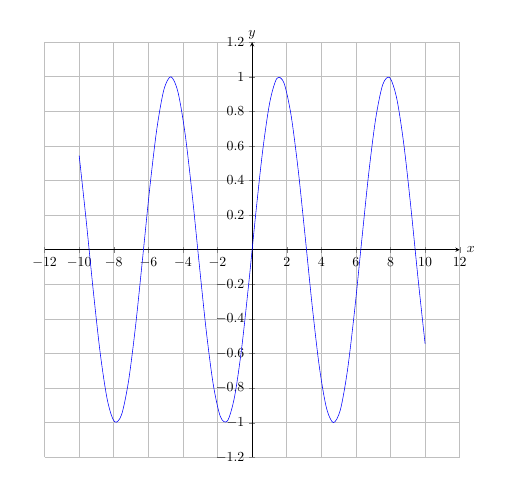
\begin{tikzpicture}[scale=.5]
		\begin{axis}[
			xmin=-10,xmax=10,
			restrict y to domain=-2:2,
			ymin=-1,ymax=1,
			grid=both,width=\textwidth,height=\textwidth,
			axis lines=middle,
			xlabel=$x$,
			ylabel=$y$,
			enlarge x limits=0.1,
			enlarge y limits=0.1,
			x label style={at={(ticklabel* cs:1.00)}, inner sep=5pt, anchor=west},
			y label style={at={(ticklabel* cs:1.00)}, inner sep=2pt, anchor=south},
		]
			\addplot[color=blue,samples=50,smooth,domain=-10:10,variable=\x]{sin(\x r)};
		\end{axis}
	\end{tikzpicture}
	\caption{正弦函数\(y=\sin x\)的图形}
	\label{figure:函数.正弦函数的图形}
\end{figure}

\begin{figure}
	\centering
	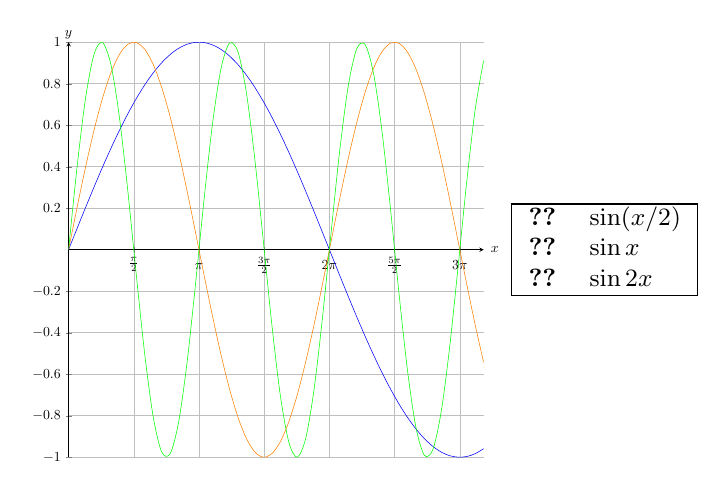
\begin{tikzpicture}[scale=.5]
		\begin{axis}[
			name=Sine,
			xmin=0,xmax=10,
			restrict y to domain=-2:2,
			ymin=-1,ymax=1,
			grid=both,width=\textwidth,height=\textwidth,
			axis lines=middle,
			xlabel=$x$,
			ylabel=$y$,
			x label style={at={(ticklabel* cs:1.00)}, inner sep=5pt, anchor=west},
			y label style={at={(ticklabel* cs:1.00)}, inner sep=2pt, anchor=south},
			xtick={0,1.5708,3.1416,...,10},
			xticklabels={
				$\relax$,
				$\frac{\pi}{2}$,
				$\pi\vphantom{\frac12}$,
				$\frac{3\pi}{2}$,
				$2\pi\vphantom{\frac12}$,
				$\frac{5\pi}{2}$,
				$3\pi\vphantom{\frac12}$,
			},
		]
			\addplot[color=blue,samples=50,smooth,domain=0:10,variable=\x]
				{sin(.5*\x r)};\label{pgfplots:正弦函数.sin(x/2)}
			\addplot[color=orange,samples=50,smooth,domain=0:10,variable=\x]
				{sin(\x r)};\label{pgfplots:正弦函数.sin(x)}
			\addplot[color=green,samples=50,smooth,domain=0:10,variable=\x]
				{sin(2*\x r)};\label{pgfplots:正弦函数.sin(2*x)}
		\end{axis}
		\node[draw,fill=white,inner sep=0pt,right=1em]at(Sine.east){\small\begin{tabular}{cl}
		\ref{pgfplots:正弦函数.sin(x/2)} & \(\sin(x/2)\) \\
		\ref{pgfplots:正弦函数.sin(x)} & \(\sin x\) \\
		\ref{pgfplots:正弦函数.sin(2*x)} & \(\sin2x\) \\
		\end{tabular}};
	\end{tikzpicture}
	\caption{}
\end{figure}

\begin{property}
如\cref{figure:函数.正弦函数的图形},
可以观察得出正弦函数的若干性质.
\begin{enumerate}
	\item 正弦函数是周期函数,其周期为\(T = 2\pi\).
	\item 正弦函数在区间\([2k\pi-\frac{\pi}{2},2k\pi+\frac{\pi}{2})\)上单调递增.
	\item 在区间\([2k\pi+\frac{\pi}{2},2k\pi+\frac{3\pi}{2})\)上单调递增.
	\item 当\(x=\frac{\pi}{2}+2k\pi\ (k\in\mathbb{Z})\)时,正弦函数\(y=\sin x\)取得极大值\(1\).
	\item 当\(x=\frac{3\pi}{2}+2k\pi\ (k\in\mathbb{Z})\)时,正弦函数\(y=\sin x\)取得极小值\(-1\).
	\item 正弦函数是奇函数,其图形关于坐标原点\(O\)中心对称,满足\(\sin(-x)=-\sin x\).
\end{enumerate}
\end{property}

\begin{figure}[htb]
	\centering
	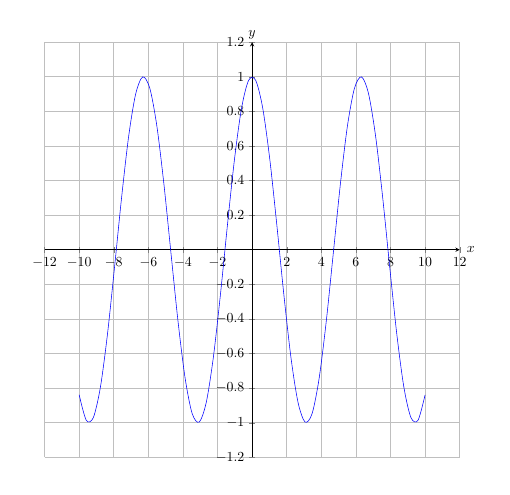
\begin{tikzpicture}[scale=.5]
		\begin{axis}[
			xmin=-10,xmax=10,
			restrict y to domain=-2:2,
			ymin=-1,ymax=1,
			grid=both,width=\textwidth,height=\textwidth,
			axis lines=middle,
			xlabel=$x$,
			ylabel=$y$,
			enlarge x limits=0.1,
			enlarge y limits=0.1,
			x label style={at={(ticklabel* cs:1.00)}, inner sep=5pt, anchor=west},
			y label style={at={(ticklabel* cs:1.00)}, inner sep=2pt, anchor=south},
		]
			\addplot[color=blue,samples=50,smooth,domain=-10:10,variable=\x]{cos(\x r)};
		\end{axis}
	\end{tikzpicture}
	\caption{余弦函数\(y=\cos x\)的图形}
	\label{figure:函数.余弦函数的图形}
\end{figure}

\begin{figure}
	\centering
	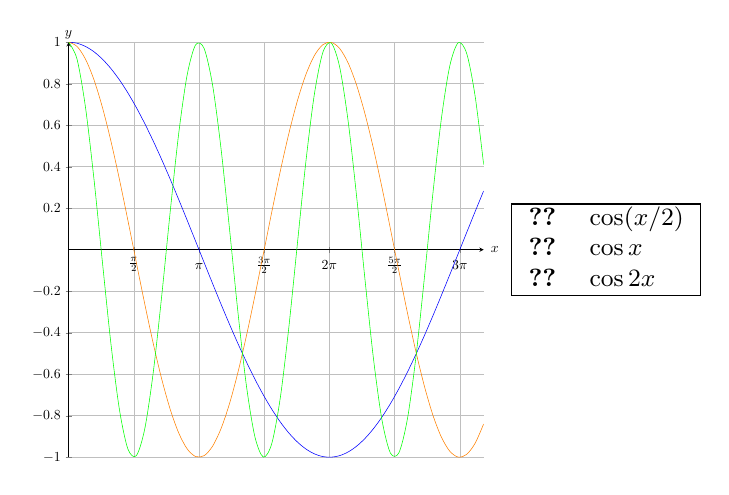
\begin{tikzpicture}[scale=.5]
		\begin{axis}[
			name=Cosine,
			xmin=0,xmax=10,
			restrict y to domain=-2:2,
			ymin=-1,ymax=1,
			grid=both,width=\textwidth,height=\textwidth,
			axis lines=middle,
			xlabel=$x$,
			ylabel=$y$,
			x label style={at={(ticklabel* cs:1.00)}, inner sep=5pt, anchor=west},
			y label style={at={(ticklabel* cs:1.00)}, inner sep=2pt, anchor=south},
			xtick={0,1.5708,3.1416,...,10},
			xticklabels={
				$\relax$,
				$\frac{\pi}{2}$,
				$\pi\vphantom{\frac12}$,
				$\frac{3\pi}{2}$,
				$2\pi\vphantom{\frac12}$,
				$\frac{5\pi}{2}$,
				$3\pi\vphantom{\frac12}$,
			},
		]
			\addplot[color=blue,samples=50,smooth,domain=0:10,variable=\x]
				{cos(.5*\x r)};\label{pgfplots:余弦函数.cos(x/2)}
			\addplot[color=orange,samples=50,smooth,domain=0:10,variable=\x]
				{cos(\x r)};\label{pgfplots:余弦函数.cos(x)}
			\addplot[color=green,samples=50,smooth,domain=0:10,variable=\x]
				{cos(2*\x r)};\label{pgfplots:余弦函数.cos(2*x)}
		\end{axis}
		\node[draw,fill=white,inner sep=0pt,right=1em]at(Cosine.east){\small\begin{tabular}{cl}
		\ref{pgfplots:余弦函数.cos(x/2)} & \(\cos(x/2)\) \\
		\ref{pgfplots:余弦函数.cos(x)} & \(\cos x\) \\
		\ref{pgfplots:余弦函数.cos(2*x)} & \(\cos2x\) \\
		\end{tabular}};
	\end{tikzpicture}
	\caption{}
\end{figure}

\begin{property}
如\cref{figure:函数.余弦函数的图形},
可以观察得出余弦函数的若干性质.
\begin{enumerate}
	\item 余弦函数也是周期函数,其周期为\(T = 2\pi\).
	\item 余弦函数在区间\([2k\pi,\pi+2k\pi)\)上单调递减.
	\item 在区间\([\pi+2k\pi,2\pi+2k\pi)\)上单调递增.
	\item 当\(x=2k\pi\ (k\in\mathbb{Z})\)时,余弦函数\(y=\cos x\)取得极大值\(1\).
	\item 当\(x=(2k-1)\pi\ (k\in\mathbb{Z})\)时,余弦函数\(y=\cos x\)取得极小值\(-1\).
	\item 余弦函数是偶函数,其图形关于\(y\)轴对称,满足\(\cos(-x)=\cos x\).
\end{enumerate}
\end{property}

\begin{figure}[htb]
	\centering
	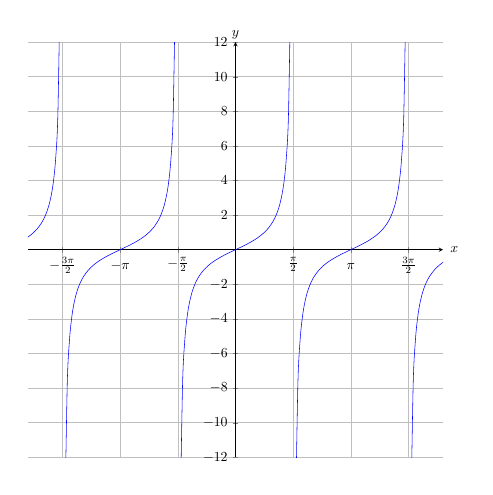
\begin{tikzpicture}[scale=.5]
		\begin{axis}[
			restrict y to domain=-20:20,
			ymin=-10,ymax=10,
			grid=both,width=\textwidth,height=\textwidth,
			axis lines=middle,
			xlabel=$x$,
			ylabel=$y$,
			enlarge x limits=0.1,
			enlarge y limits=0.1,
			x label style={at={(ticklabel* cs:1.00)}, inner sep=5pt, anchor=west},
			y label style={at={(ticklabel* cs:1.00)}, inner sep=2pt, anchor=south},
			xmin=-4.7124, xmax=4.7124,
			xtick={-4.7124,-3.1416,-1.5708,...,10},
			xticklabels={
				$-\frac{3\pi}{2}$,
				$-\pi\vphantom{\frac{1}{2}}$,
				$-\frac{\pi}{2}$,
				$\relax$,%不能去掉\relax
				$\frac{\pi}{2}$,
				$\pi\vphantom{\frac{1}{2}}$,
				$\frac{3\pi}{2}$,
			},
		]
			\foreach \i in {-5,-3,...,3} {
				\addplot[color=blue,samples=50,smooth,domain={\i*pi/2}:{(\i+2)*pi/2},variable=\x]
				{tan(\x r)};
			}
		\end{axis}
	\end{tikzpicture}
	\caption{正切函数\(y=\tan x\)的图形}
	\label{figure:函数.正切函数的图形}
\end{figure}

\begin{property}
如\cref{figure:函数.正切函数的图形},
可以观察得出正切函数的若干性质.
\begin{enumerate}
	\item 正切函数是周期函数,其周期为\(T = \pi\).
	\item 正切函数在区间\((k\pi-\frac{\pi}{2},k\pi+\frac{\pi}{2})\ (k\in\mathbb{Z})\)上单调递增.
	\item 正切函数是奇函数,其图形关于坐标原点\(O\)中心对称,满足\(\tan(-x)=-\tan x\).
\end{enumerate}
\end{property}

\begin{figure}[htb]
	\centering
	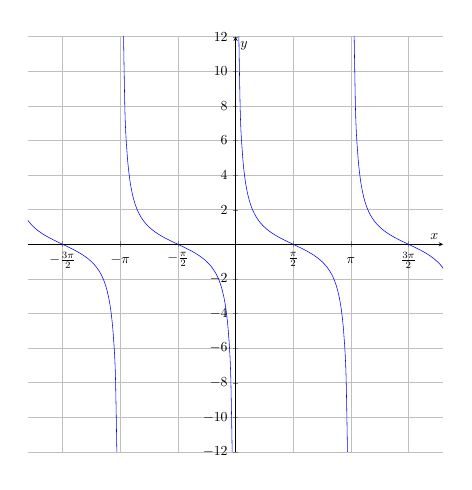
\begin{tikzpicture}[scale=.5]
		\begin{axis}[
			restrict y to domain=-20:20,
			ymin=-10,ymax=10,
			grid=both,width=\textwidth,height=\textwidth,
			axis lines=middle,
			xlabel=$x$,
			ylabel=$y$,
			enlarge x limits=0.1,
			enlarge y limits=0.1,
			xmin=-4.7124, xmax=4.7124,
			xtick={-4.7124,-3.1416,-1.5708,...,10},
			xticklabels={
				$-\frac{3\pi}{2}$,
				$-\pi\vphantom{\frac{1}{2}}$,
				$-\frac{\pi}{2}$,
				$\relax$,%不能去掉\relax
				$\frac{\pi}{2}$,
				$\pi\vphantom{\frac{1}{2}}$,
				$\frac{3\pi}{2}$,
			},
		]
		\foreach \i in {-2,-1,0,1} {
			\addplot[color=blue,samples=50,smooth,domain={\i*pi}:{(\i+1)*pi},variable=\x]
			{cot(\x r)};
		}
		\end{axis}
	\end{tikzpicture}
	\caption{余切函数\(y=\cot x\)的图形}
\end{figure}

\begin{table}[htb]
	\centering
	\begin{tblr}{*2c}
		\hline
		函数 & 周期 \\
		\hline
		\(\sin(\omega x)\) & \(\frac{2\pi}{\omega}\) \\
		\(\cos(\omega x)\) & \(\frac{2\pi}{\omega}\) \\
		\(\tan(\omega x)\) & \(\frac{\pi}{\omega}\) \\
		\(\cot(\omega x)\) & \(\frac{\pi}{\omega}\) \\
		\(\sec(\omega x)\) & \(\frac{2\pi}{\omega}\) \\
		\(\csc(\omega x)\) & \(\frac{2\pi}{\omega}\) \\
		\hline
	\end{tblr}
	\caption{角速度$\omega$与三角函数的周期的关系}
\end{table}

\subsection{和积互化公式}
\begin{theorem}[和积互化公式]
设\(\alpha,\beta\in\mathbb{R}\),则有
\begin{gather}
	\sin(\alpha\pm\beta) = \sin\alpha\cos\beta\pm\cos\alpha\sin\beta,
	\label{equation:函数.三角函数.和积互化公式1} \\
	\cos(\alpha\pm\beta) = \cos\alpha\cos\beta\mp\sin\alpha\sin\beta,
	\label{equation:函数.三角函数.和积互化公式2} \\
	\tan(\alpha\pm\beta) = \frac{\tan\alpha\pm\tan\beta}{1\mp\tan\alpha\tan\beta},
	\label{equation:函数.三角函数.和积互化公式3} \\
	\cot(\alpha\pm\beta) = \frac{\cot\alpha\cot\beta\mp 1}{\cot\beta\pm\cot\alpha},
	\label{equation:函数.三角函数.和积互化公式4} \\
	\sec(\alpha\pm\beta) = \frac{\sec\alpha\sec\beta}{1\mp\tan\alpha\tan\beta},
	\label{equation:函数.三角函数.和积互化公式5} \\
	\csc(\alpha\pm\beta) = \frac{\csc\alpha\csc\beta}{\cot\beta\pm\cot\alpha},
	\label{equation:函数.三角函数.和积互化公式6} \\
	\sin \alpha \cos \beta = \frac{\sin (\alpha + \beta) + \sin (\alpha - \beta)}{2},
	\label{equation:函数.三角函数.和积互化公式7} \\
	\cos \alpha \sin \beta = \frac{\sin (\alpha + \beta) - \sin (\alpha - \beta)}{2},
	\label{equation:函数.三角函数.和积互化公式8} \\
	\cos \alpha \cos \beta = \frac{\cos (\alpha + \beta) + \cos (\alpha - \beta)}{2},
	\label{equation:函数.三角函数.和积互化公式9} \\
	\sin \alpha \sin \beta = -\frac{\cos (\alpha + \beta) - \cos (\alpha - \beta)}{2},
	\label{equation:函数.三角函数.和积互化公式10} \\
	\sin \alpha + \sin \beta = 2 \sin \frac{\alpha + \beta}{2} \cos \frac{\alpha - \beta}{2},
	\label{equation:函数.三角函数.和积互化公式11} \\
	\sin \alpha - \sin \beta = 2 \cos \frac{\alpha + \beta}{2} \sin \frac{\alpha - \beta}{2},
	\label{equation:函数.三角函数.和积互化公式12} \\
	\cos \alpha + \cos \beta = 2 \cos \frac{\alpha + \beta}{2} \cos \frac{\alpha - \beta}{2},
	\label{equation:函数.三角函数.和积互化公式13} \\
	\cos \alpha - \cos \beta = -2 \sin \frac{\alpha + \beta}{2} \sin \frac{\alpha - \beta}{2}.
	\label{equation:函数.三角函数.和积互化公式14}
\end{gather}
\begin{proof}
\begin{figure}[htb]
	\centering
	\begin{tikzpicture}
		\coordinate(A)at(0.0,0.0);
		\coordinate(B)at(6.4,0.0);
		\coordinate(C)at(6.4,4.8);
		\coordinate(D)at(6.4,6.4);
		\coordinate(E)at(5.2,6.4);
		\draw (A)
			--(B)node[midway,below]{\(\cos\alpha\cos\beta\)}
			--(C)node[midway,right]{\rotatebox{90}{\(\cos\alpha\sin\beta\)}}
			--(D)node[midway,right]{\rotatebox{90}{\(\sin\alpha\cos\beta\)}}
			--(E)node[midway,above]{\(\sin\alpha\sin\beta\)}
			--(C)node[midway,left=2mm,below=-3mm]{\rotatebox{-53.13}{\(\sin\alpha\)}}
			--(A)node[midway,right=1mm,below=-2mm]{\rotatebox{36.87}{\(\cos\alpha\)}}
			--(E)node[midway,left=2mm,above=2mm]{\(1\)};
		\pic["\(\alpha\)",draw=orange,-,angle eccentricity=2,angle radius=0.7cm]{angle=C--A--E};
		\pic["\(\beta\)",draw=blue,-,angle eccentricity=2,angle radius=0.7cm]{angle=B--A--C};
		\pic[draw=blue,-,angle radius=0.5cm]{angle=D--C--E};
		\pic[draw=gray,-,angle radius=0.3cm]{right angle=C--B--A};
		\pic[draw=gray,-,angle radius=0.3cm]{right angle=E--C--A};
		\pic[draw=gray,-,angle radius=0.3cm]{right angle=E--D--C};
	\end{tikzpicture}
	\caption{和积互化公式的辅助三角形}
	\label{figure:函数.和积互化公式的辅助三角形}
\end{figure} %

观察\cref{figure:函数.和积互化公式的辅助三角形} 可知
\begin{align*}
	\sin(\alpha+\beta) &= \sin\alpha\cos\beta+\cos\alpha\sin\beta, \\
	\cos(\alpha+\beta) &= \cos\alpha\cos\beta-\sin\alpha\sin\beta
\end{align*}成立.
又令\(\beta=-\beta\)则可得
\begin{align*}
	\sin(\alpha-\beta) &= \sin\alpha\cos\beta-\cos\alpha\sin\beta, \\
	\cos(\alpha-\beta) &= \cos\alpha\cos\beta+\sin\alpha\sin\beta.
\end{align*}

计算\(\sin(\alpha\pm\beta)\)除以\(\cos(\alpha\pm\beta)\)便得\begin{align*}
	\tan(\alpha\pm\beta)
	&= \frac{\sin(\alpha\pm\beta)}{\cos(\alpha\pm\beta)}
	= \frac{\sin\alpha\cos\beta\pm\cos\alpha\sin\beta}
		{\cos\alpha\cos\beta\mp\sin\alpha\sin\beta} \\
	&\xlongequal{\text{分子分母同除以$\cos\alpha\cos\beta$}}
		\frac{\tan\alpha\pm\tan\beta}{1\mp\tan\alpha\tan\beta}.
\end{align*}

计算\(\cos(\alpha\pm\beta)\)除以\(\sin(\alpha\pm\beta)\)便得\begin{align*}
	\cot(\alpha\pm\beta)
	&= \frac{\cos(\alpha\pm\beta)}{\sin(\alpha\pm\beta)}
	= \frac{\cos\alpha\cos\beta\mp\sin\alpha\sin\beta}
		{\sin\alpha\cos\beta\pm\cos\alpha\sin\beta} \\
	&\xlongequal{\text{分子分母同除以$\sin\alpha\sin\beta$}}
		\frac{\cot\alpha\cot\beta\mp1}{\cot\beta\pm\cot\alpha}.
\end{align*}

计算\(\cos(\alpha\pm\beta)\)的倒数得\[
	\sec(\alpha\pm\beta)
	= \frac1{\cos(\alpha\pm\beta)}
	\xlongequal{\text{分子分母同除以$\cos\alpha\cos\beta$}}
		\frac{\sec\alpha\sec\beta}{1\mp\tan\alpha\tan\beta}.
\]

计算\(\sin(\alpha\pm\beta)\)的倒数得\[
	\csc(\alpha\pm\beta)
	= \frac1{\sin(\alpha\pm\beta)}
	\xlongequal{\text{分子分母同除以$\sin\alpha\sin\beta$}}
		\frac{\csc\alpha\csc\beta}{\cot\beta\pm\cot\alpha}.
\]

把\(\sin(\alpha+\beta) = \sin\alpha\cos\beta+\cos\alpha\sin\beta\)
与\(\sin(\alpha-\beta) = \sin\alpha\cos\beta-\cos\alpha\sin\beta\)
相加便得\[
	2\sin\alpha\cos\beta = \sin(\alpha+\beta) + \sin(\alpha-\beta),
\]
于是\[
	\sin\alpha\cos\beta = \frac{\sin(\alpha+\beta) + \sin(\alpha-\beta)}2.
\]

把\(\sin(\alpha+\beta) = \sin\alpha\cos\beta+\cos\alpha\sin\beta\)
与\(\sin(\alpha-\beta) = \sin\alpha\cos\beta-\cos\alpha\sin\beta\)
相减便得\[
	2\cos\alpha\sin\beta = \sin(\alpha+\beta) - \sin(\alpha-\beta),
\]
于是\[
	\cos\alpha\sin\beta = \frac{\sin(\alpha+\beta) - \sin(\alpha-\beta)}2.
\]

把\(\cos(\alpha+\beta) = \cos\alpha\cos\beta-\sin\alpha\sin\beta\)
与\(\cos(\alpha-\beta) = \cos\alpha\cos\beta+\sin\alpha\sin\beta\)
分别相加、相减便得\begin{gather*}
	2\cos\alpha\cos\beta = \cos(\alpha+\beta) + \cos(\alpha-\beta), \\
	-2\sin\alpha\sin\beta = \cos(\alpha+\beta) - \cos(\alpha-\beta),
\end{gather*}
于是\begin{gather*}
	\cos\alpha\cos\beta = \frac{\cos(\alpha+\beta) + \cos(\alpha-\beta)}2, \\
	\sin\alpha\sin\beta = \frac{\cos(\alpha-\beta) - \cos(\alpha+\beta)}2.
\end{gather*}

在\(2\sin\alpha\cos\beta = \sin(\alpha+\beta) + \sin(\alpha-\beta)\)中
用\(x\)代\(\alpha+\beta\),用\(y\)代\(\alpha-\beta\),
于是\[
	\sin x + \sin y = 2 \sin\frac{x+y}2 \cos\frac{x-y}2.
\]

在\(2\cos\alpha\sin\beta = \sin(\alpha+\beta) - \sin(\alpha-\beta)\)中
用\(x\)代\(\alpha+\beta\),用\(y\)代\(\alpha-\beta\),
于是\[
	\sin x - \sin y = 2 \cos\frac{x+y}2 \sin\frac{x-y}2.
\]

在\(2\cos\alpha\cos\beta = \cos(\alpha+\beta) + \cos(\alpha-\beta)\)中
用\(x\)代\(\alpha+\beta\),用\(y\)代\(\alpha-\beta\),
于是\[
	\cos x + \cos y = 2 \cos\frac{x+y}2 \cos\frac{x-y}2.
\]

在\(-2\sin\alpha\sin\beta = \cos(\alpha+\beta) - \cos(\alpha-\beta)\)中
用\(x\)代\(\alpha+\beta\),用\(y\)代\(\alpha-\beta\),
于是\[
	\cos x - \cos y = -2 \sin\frac{x+y}2 \sin\frac{x-y}2.
	\qedhere
\]
\end{proof}
\end{theorem}

特别地,根据和积互化公式有\begin{gather}
	\sin(-\alpha) = -\sin\alpha, \\
	\cos(-\alpha) = \cos\alpha, \\
	\tan(-\alpha) = -\tan\alpha, \\
	\sec(-\alpha) = \sec\alpha, \\
	\csc(-\alpha) = -\csc\alpha, \\
	\cot(-\alpha) = -\cot\alpha, \\
	\sin(\alpha+2n\pi) = \sin\alpha, \\
	\cos(\alpha+2n\pi) = \cos\alpha, \\
	\tan(\alpha+n\pi) = \tan\alpha, \\
	\sec(\alpha+2n\pi) = \sec\alpha, \\
	\csc(\alpha+2n\pi) = \csc\alpha, \\
	\cot(\alpha+n\pi) = \cot\alpha, \\
	\sin(\pi+\alpha) = -\sin\alpha,
		\label{equation:函数.三角函数.诱导公式1} \\
	\cos(\pi+\alpha) = -\cos\alpha,
		\label{equation:函数.三角函数.诱导公式2} \\
	\tan(\pi+\alpha) = \tan\alpha,
		\label{equation:函数.三角函数.诱导公式3} \\
	\cot(\pi+\alpha) = \cot\alpha,
		\label{equation:函数.三角函数.诱导公式4} \\
	\sin(\pi-\alpha) = \sin\alpha,
		\label{equation:函数.三角函数.诱导公式5} \\
	\cos(\pi-\alpha) = -\cos\alpha,
		\label{equation:函数.三角函数.诱导公式6} \\
	\tan(\pi-\alpha) = -\tan\alpha,
		\label{equation:函数.三角函数.诱导公式7} \\
	\cot(\pi-\alpha) = -\cot\alpha.
		\label{equation:函数.三角函数.诱导公式8}
\end{gather}
还有\begin{gather}
	\cos\left(\frac{\pi}{2}-\alpha\right) = \sin\alpha,
		\label{equation:函数.三角函数.诱导公式9} \\
	\sin\left(\frac{\pi}{2}-\alpha\right) = \cos\alpha,
		\label{equation:函数.三角函数.诱导公式10} \\
	\tan\left(\frac{\pi}{2}-\alpha\right) = \cot\alpha,
		\label{equation:函数.三角函数.诱导公式11} \\
	\cot\left(\frac{\pi}{2}-\alpha\right) = \tan\alpha.
		\label{equation:函数.三角函数.诱导公式12}
\end{gather}
以上四个公式是当\(\alpha\)为任意角时
\(\left(\frac{\pi}{2}-\alpha\right)\)的诱导公式.
如果把其中的\(\alpha\)换成\((-\alpha)\),
就可得到当\(\alpha\)为任意角时
\(\left(\frac{\pi}{2}+\alpha\right)\)的诱导公式:
\begin{gather}
	\cos\left(\frac{\pi}{2}+\alpha\right) = -\sin\alpha,
		\label{equation:函数.三角函数.诱导公式13} \\
	\sin\left(\frac{\pi}{2}+\alpha\right) = \cos\alpha,
		\label{equation:函数.三角函数.诱导公式14} \\
	\tan\left(\frac{\pi}{2}+\alpha\right) = -\cot\alpha,
		\label{equation:函数.三角函数.诱导公式15} \\
	\cot\left(\frac{\pi}{2}+\alpha\right) = -\tan\alpha.
		\label{equation:函数.三角函数.诱导公式16}
\end{gather}

%\begin{example}
%\def\s{\sum_{k=1}^n}%
%证明:
%当\(x\neq0\)时,有
%\begin{gather}
%	\s \sin kx
%	= \frac{\sin\frac{nx}{2} \sin\frac{(n+1)x}{2}}{\sin\frac{x}{2}}, \\
%	\s \cos kx
%	= \frac{\sin\frac{nx}{2} \cos\frac{(n+1)x}{2}}{\sin\frac{x}{2}}.
%\end{gather}
%TODO
%\end{example}

\subsection{倍角公式}
\begin{proposition}[二倍角公式]
设\(\alpha\in\mathbb{R}\),则有
\begin{align}
	\sin2\alpha &= 2 \sin\alpha \cos\alpha,
		\label{equation:三角函数.正弦的二倍角公式} \\
	\cos2\alpha &= \cos^2\alpha - \sin^2\alpha
		\label{equation:三角函数.余弦的二倍角公式1} \\
		&= 2 \cos^2\alpha - 1 \\
		&= 1 - 2 \sin^2\alpha, \\
	\tan2\alpha &= \frac{2 \tan\alpha}{1 - \tan^2\alpha}.
		\label{equation:三角函数.正切的二倍角公式}
\end{align}
\begin{proof}
在\cref{equation:函数.三角函数.和积互化公式1,equation:函数.三角函数.和积互化公式2} 中,
令\(\beta=\alpha\),就有\[
	\sin2\alpha
	=\sin(\alpha+\alpha)
	=\sin\alpha\cos\alpha+\cos\alpha\sin\alpha
	=2\sin\alpha\cos\alpha,
	\eqno(1)
\]\[
	\cos2\alpha
	=\cos(\alpha+\alpha)
	=\cos\alpha\cos\alpha-\sin\alpha\sin\alpha
	=\cos^2\alpha-\sin^2\alpha.
	\eqno(2)
\]
考虑到\cref{equation:三角函数.毕达哥拉斯三角恒等式1},
\(\sin^2\alpha+\cos^2\alpha=1\),
于是(2)又可以化为以下两种形式:\[
	\cos2\alpha
	=(\cos^2\alpha-\sin^2\alpha)+(1-\sin^2\alpha-\cos^2\alpha)
	=1-2\sin^2\alpha,
\]\[
	\cos2\alpha
	=(\cos^2\alpha-\sin^2\alpha)+(\sin^2\alpha+\cos^2\alpha-1)
	=2\cos^2\alpha-1.
\]
接着只需要将(1)式与(2)式等号两边分别相除,得\[
	\tan2\alpha=\frac{\sin2\alpha}{\cos2\alpha}
	=\frac{2\sin\alpha\cos\alpha}{cos^2\alpha-\sin^2\alpha}
	=\frac{(2\sin\alpha\cos\alpha)/\cos^2\alpha}
		{(\cos^2\alpha-\sin^2\alpha)/\cos^2\alpha}
	=\frac{2\tan\alpha}{1-\tan^2\alpha}.
	\qedhere
\]
\end{proof}
\end{proposition}

\begin{proposition}
设\(\alpha\in\mathbb{R}\),则有\begin{align}
	\sin3\alpha &= 3 \sin\alpha - 4 \sin^3\alpha. \\
	\cos3\alpha &= 4 \cos^3\alpha - 3 \cos\alpha. \\
	\tan3\alpha &= \frac{3 \tan\alpha - \tan^3\alpha}{1 - 3\tan^2\alpha}.
\end{align}
\begin{proof}
直接计算得\begin{align*}
	\sin3\alpha &= \sin(\alpha+2\alpha)
	= \sin\alpha\cos2\alpha + \cos\alpha\sin2\alpha \\
	&= \sin\alpha(1-2\sin^2\alpha)
		+ \cos\alpha(2\sin\alpha\cos\alpha) \\
	&= \sin\alpha-2\sin^3\alpha
		+ 2\sin\alpha(1-\sin^2\alpha) \\
	&= 3\sin\alpha-4\sin^3\alpha. \\
	\cos3\alpha &= \cos(\alpha+2\alpha)
	= \cos\alpha\cos2\alpha - \sin\alpha\sin2\alpha \\
	&= \cos\alpha(2\cos^2\alpha-1) - \sin\alpha(2\sin\alpha\cos\alpha) \\
	&= 2\cos^3\alpha - \cos\alpha
		- 2(1-\cos^2\alpha)\cos\alpha \\
	&= 4\cos^3\alpha - 3\cos\alpha.
	\qedhere
\end{align*}
%TODO proof
\end{proof}
\end{proposition}

\begin{proposition}[半倍角公式]
\begin{align}
	\sin\frac\alpha2 &= \pm \sqrt{\frac{1 - \cos\alpha}{2}},
		\label{equation:三角函数.正弦的半倍角公式} \\
	\cos\frac\alpha2 &= \pm \sqrt{\frac{1 + \cos\alpha}{2}}, \\
	\tan\frac\alpha2
	&= \frac{\sin\alpha}{1+\cos\alpha} \\
	&= \frac{1-\cos\alpha}{\sin\alpha} \\
	&= \pm \sqrt{\frac{1 - \cos\alpha}{1 + \cos\alpha}}.
\end{align}
以上公式中的正负号的选择由\(\frac\alpha2\)所在的象限决定.
\begin{proof}
联立\[
	\left\{ \begin{array}{l}
		\cos^2\alpha - \sin^2\alpha = \cos 2\alpha, \\
		\cos^2\alpha + \sin^2\alpha = 1,
	\end{array} \right.
\]
整理得\[
	2\cos^2\alpha=1+\cos2\alpha, \qquad
	2\sin^2\alpha=1-\cos2\alpha,
\]
即\[
	\cos^2\alpha=\frac{1+\cos2\alpha}{2}, \qquad
	\sin^2\alpha=\frac{1-\cos2\alpha}{2},
\]
在等号两边同时开方,得\[
	\cos\alpha = \pm\sqrt{\frac{1+\cos2\alpha}{2}}, \qquad
	\sin\alpha = \pm\sqrt{\frac{1-\cos2\alpha}{2}},
\]
再相除可得\[
	\tan\alpha = \frac{\sin\alpha}{\cos\alpha}
	= \pm \sqrt{\frac{1 - \cos2\alpha}{1 + \cos2\alpha}}.
	\qedhere
\]
\end{proof}
\end{proposition}

\begin{figure}[htb]
	\centering
	\begin{tikzpicture}[scale=4]
		\pgfmathsetmacro{\t}{60}
		\coordinate(C)at({cos(\t)},{sin(\t)});
		\draw(1,0)coordinate(A)node[right]{\(A\)}
			arc[start angle=0,end angle=180,radius=1]
			coordinate(B)node[left]{\(B\)}--(0,0)coordinate(O)node[below]{\(O\)}
			--(C)node[above right]{\(C\)};
		\draw(C)--(C|-A)coordinate(D)node[below]{\(D\)}
			node[midway,above,rotate=90,orange]{\(\sin\theta\)};
		\draw(O)--(D)node[midway,below,orange]{\(\cos\theta\)}
			--(A)node[midway,below,orange]{\(1-\cos\theta\)}
			--(C)--(B)--(O)node[midway,below,orange]{\(1\)}
			pic[draw=gray,angle radius=0.3cm]{right angle=A--D--C}
			pic[draw=gray,angle radius=0.3cm]{right angle=B--C--A}
			pic["$\frac{\theta}{2}$",draw=cyan,angle eccentricity=1.7,angle radius=5mm]{angle=D--C--A}
			pic["$\frac{\theta}{2}$",draw=cyan,angle eccentricity=1.7,angle radius=5mm]{angle=A--B--C}
			pic["$\theta$",draw=blue,angle eccentricity=1.7,angle radius=5mm]{angle=D--O--C};
	\end{tikzpicture}
	\caption{半角公式的辅助三角形}
	\label{figure:函数.半角公式的辅助三角形}
\end{figure}

\begin{proposition}[万能公式]
\def\HalfAlpha{\frac\alpha2}
设\(\alpha\in\mathbb{R}\),则有
\begin{gather}
	\sin\alpha = \frac{2 \tan\HalfAlpha}{1+\tan^2\HalfAlpha},
		\label{equation:三角函数.万能公式1} \\
	\cos\alpha = \frac{1-\tan^2\HalfAlpha}{1+\tan^2\HalfAlpha},
		\label{equation:三角函数.万能公式2} \\
	\tan\alpha = \frac{2 \tan\HalfAlpha}{1-\tan^2\HalfAlpha}.
		\label{equation:三角函数.万能公式3}
\end{gather}
\begin{proof}
由\cref{equation:三角函数.正切的二倍角公式} 立即可得\[
	\tan\alpha
	=\frac{2\tan\HalfAlpha}{1-\tan^2\HalfAlpha}.
\]
由\cref{equation:三角函数.正弦的二倍角公式,equation:三角函数.余弦的二倍角公式1} 可得\[
	\sin\alpha
	=2\sin\HalfAlpha\cos\HalfAlpha
	=\frac{2\sin\HalfAlpha\cos\HalfAlpha}{\cos^2\HalfAlpha+\sin^2\HalfAlpha}
	=\frac{2\tan^2\HalfAlpha}{1+\tan^2\HalfAlpha},
\]\[
	\cos\alpha
	=\cos^2\HalfAlpha-\sin^2\HalfAlpha
	=\frac{\cos^2\HalfAlpha-\sin^2\HalfAlpha}{\cos^2\HalfAlpha+\sin^2\HalfAlpha}
	=\frac{1-\tan^2\HalfAlpha}{1+\tan^2\HalfAlpha}.
	\qedhere
\]
\end{proof}
\end{proposition}

\subsection{辅助角公式}
\begin{proposition}[辅助角公式]
设\(x\in\mathbb{R}\),
\(a,b\in\mathbb{R}^*\),
成立\begin{equation}
	a \sin x + b \cos x = \sqrt{a^2 + b^2} \sin(x + \phi),
\end{equation}
其中\(tan\phi = \frac{b}{a}\).
\begin{proof}
显然\[
	a \sin x + b \cos x
	= \sqrt{a^2 + b^2} \left(
		\frac{a}{\sqrt{a^2 + b^2}} \sin x
		+ \frac{b}{\sqrt{a^2 + b^2}} \cos x
	\right).
\]
令\(\cos\phi = \frac{a}{\sqrt{a^2 + b^2}},
\sin\phi = \frac{b}{\sqrt{a^2 + b^2}}\),
那么\begin{equation*}
	\frac{a}{\sqrt{a^2 + b^2}} \sin x
	+ \frac{b}{\sqrt{a^2 + b^2}} \cos x
	= \cos\phi \sin x + \sin\phi \cos x
	= \sin(x + \phi)
\end{equation*}
并且有\[
	\frac{b}{a}
	= \frac{\sqrt{a^2 + b^2} \sin\phi}{\sqrt{a^2 + b^2} \cos\phi}
	= \tan\phi.
	\qedhere
\]
\end{proof}
\end{proposition}

\subsection{正(余)弦函数的一般形式}
\begin{definition}
一般地,把函数\[
F(t) = A \sin(\omega t + \phi) \quad (-\infty<t<+\infty)
\]称作正弦函数的一般形式,其中\(A\)称为\DefineConcept{振幅},\(\omega\)称为\DefineConcept{角速度},\(\phi\)称为\DefineConcept{初相},\((\omega t + \phi)\)称为\DefineConcept{相位},\(T = \frac{2\pi}{\omega}\)称为\DefineConcept{最小正周期},\(f = \frac{1}{T}\)称为\DefineConcept{频率}.
\end{definition}
%@Mathematica: Manipulate[Plot[A Sin[\[Omega] x + \[Phi]], {x, 0, 2 \[Pi]}], {A, 1, 5, 1}, {\[Omega], .1, 2, .1}, {\[Phi], 0, 2 \[Pi], \[Pi]/10}]
可以证明,随着\(A\)的增大,函数\(F(t)\)的波峰(或波谷)会变得更高(或更低);而随着\(\omega\)的增大,在固定长度的区间\([0,2\pi]\)上函数\(F(t)\)出现零点的次数会变多,形象地说,就是函数\(F(t)\)的图形变密了;另外,随着\(\phi\)的增大,看起来,函数\(f(t)\)的图形好像沿着\(x\)轴向左移动一样.

\section{反三角函数}
\subsection{反三角函数的概念}
函数\(y = \sin x\ (-\frac\pi2 \leq x \leq \frac\pi2)\)的反函数,
叫做\DefineConcept{反正弦函数},
记作\(\arcsin x\).

函数\(y = \cos x\ (0 \leq x \leq \pi)\)的反函数,
叫做\DefineConcept{反余弦函数},
记作\(\arccos x\).

函数\(y = \tan x\ (-\frac\pi2 < x < \frac\pi2)\)的反函数,
叫做\DefineConcept{反正切函数},
记作\(\arctan x\).

正弦函数、余弦函数、正切函数、余切函数等三角函数的反函数,统称为\DefineConcept{反三角函数}.

\begin{figure}[htb]
	\centering
	\begin{tikzpicture}[scale=.5]
		\begin{axis}[
			xmin=-2,xmax=2,
			ymin=-2,ymax=2,
			grid=both,width=\textwidth,height=\textwidth,
			axis lines=middle,
			xlabel=$x$,
			ylabel=$y$,
			enlarge x limits=0.1,
			enlarge y limits=0.1,
			x label style={at={(ticklabel* cs:1.00)}, inner sep=5pt, anchor=west},
			y label style={at={(ticklabel* cs:1.00)}, inner sep=2pt, anchor=south},
			ytick={-1.5708,1.5708},
			yticklabels={
				$-\frac{\pi}{2}$,
				$\frac{\pi}{2}$,
			},
			xtick={-1,1},
			xticklabels={
				$-1$,
				$1$,
			}
		]
			\addplot[color=blue,samples=50,smooth,domain=-1:1,variable=\x]{asin(\x)/180*pi};
		\end{axis}
	\end{tikzpicture}
	\caption{反正弦函数\(y=\arcsin x\)的图形}
	\label{figure:函数.反正弦函数的图形}
\end{figure}

\begin{figure}[htb]
	\centering
	\begin{tikzpicture}[scale=.5]
		\begin{axis}[
			xmin=-2,xmax=2,
			ymin=0,ymax=3.5,
			grid=both,width=\textwidth,height=\textwidth,
			axis lines=middle,
			xlabel=$x$,
			ylabel=$y$,
			enlarge x limits=0.1,
			enlarge y limits=0.1,
			x label style={at={(ticklabel* cs:1.00)}, inner sep=5pt, anchor=west},
			y label style={at={(ticklabel* cs:1.00)}, inner sep=2pt, anchor=south},
			ytick={1.5708,3.1416},
			yticklabels={
				$\frac{\pi}{2}$,
				$\pi$,
			},
			xtick={-1,1},
		]
			\addplot[color=blue,samples=50,smooth,domain=-1:1,variable=\x]{acos(\x)/180*pi};
		\end{axis}
	\end{tikzpicture}
	\caption{反余弦函数\(y=\arccos x\)的图形}
	\label{figure:函数.反余弦函数的图形}
\end{figure}

\begin{figure}[htb]
	\centering
	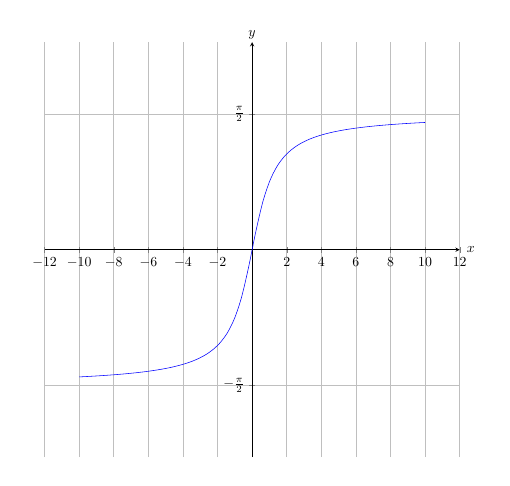
\begin{tikzpicture}[scale=.5]
		\begin{axis}[
			xmin=-10,xmax=10,
			ymin=-2,ymax=2,
			grid=both,width=\textwidth,height=\textwidth,
			axis lines=middle,
			xlabel=$x$,
			ylabel=$y$,
			enlarge x limits=0.1,
			enlarge y limits=0.1,
			x label style={at={(ticklabel* cs:1.00)}, inner sep=5pt, anchor=west},
			y label style={at={(ticklabel* cs:1.00)}, inner sep=2pt, anchor=south},
			ytick={-1.5708,1.5708},
			yticklabels={
				$-\frac{\pi}{2}$,
				$\frac{\pi}{2}$,
			},
		]
			\addplot[color=blue,samples=50,smooth,domain=-10:10,variable=\x]{atan(\x)/180*pi};
		\end{axis}
	\end{tikzpicture}
	\caption{反正切函数\(y=\arctan x\)的图形}
	\label{figure:函数.反正切函数的图形}
\end{figure}

\begin{figure}[htb]
	\centering
	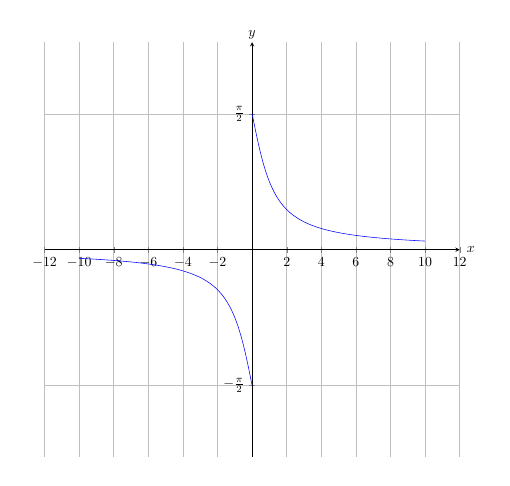
\begin{tikzpicture}[scale=.5]
		\begin{axis}[
			xmin=-10,xmax=10,
			ymin=-2,ymax=2,
			grid=both,width=\textwidth,height=\textwidth,
			axis lines=middle,
			xlabel=$x$,
			ylabel=$y$,
			enlarge x limits=0.1,
			enlarge y limits=0.1,
			x label style={at={(ticklabel* cs:1.00)}, inner sep=5pt, anchor=west},
			y label style={at={(ticklabel* cs:1.00)}, inner sep=2pt, anchor=south},
			ytick={-1.5708,1.5708},
			yticklabels={
				$-\frac{\pi}{2}$,
				$\frac{\pi}{2}$,
			},
		]
			\addplot[color=blue,samples=50,smooth,domain=0:10,variable=\x]{pi/2-atan(\x)/180*pi};
			\addplot[color=blue,samples=50,smooth,domain=-10:0,variable=\x]{-pi/2-atan(\x)/180*pi};
		\end{axis}
	\end{tikzpicture}
	\caption{反余切函数\(y=\arccot x\)的图形}
\end{figure}

\begin{figure}[htb]
	\centering
	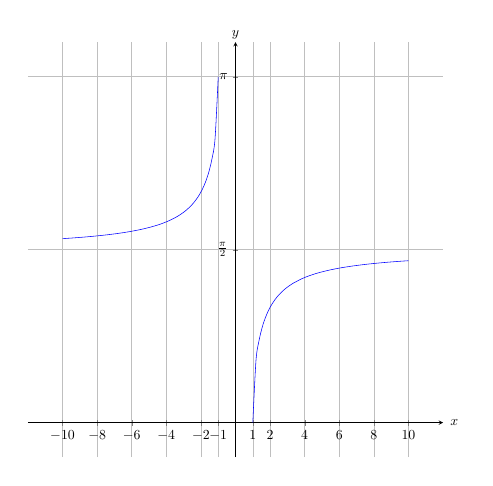
\begin{tikzpicture}[scale=.5]
		\begin{axis}[
			xmin=-10,xmax=10,
			ymin=0,ymax=pi,
			grid=both,width=\textwidth,height=\textwidth,
			axis lines=middle,
			xlabel=$x$,
			ylabel=$y$,
			enlarge x limits=0.1,
			enlarge y limits=0.1,
			x label style={at={(ticklabel* cs:1.00)}, inner sep=5pt, anchor=west},
			y label style={at={(ticklabel* cs:1.00)}, inner sep=2pt, anchor=south},
			xtick={-10,-8,...,-2,-1,1,2,4,...,10},
			ytick={1.5708,3.1416},
			yticklabels={
				$\frac{\pi}{2}$,
				$\pi$,
			},
		]
			\addplot[color=blue,samples=50,smooth,domain=1:10,variable=\x]{acos(1/\x)/180*pi};
			\addplot[color=blue,samples=50,smooth,domain=-10:-1,variable=\x]{acos(1/\x)/180*pi};
		\end{axis}
	\end{tikzpicture}
	\caption{反正割函数\(y=\arcsec x\)的图形}
\end{figure}

\begin{figure}[htb]
	\centering
	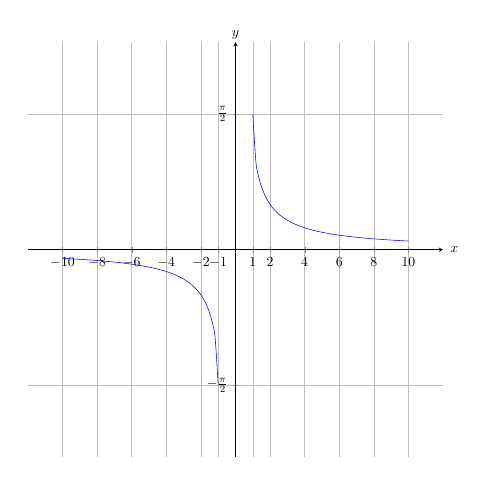
\begin{tikzpicture}[scale=.5]
		\begin{axis}[
			xmin=-10,xmax=10,
			ymin=-2,ymax=2,
			grid=both,width=\textwidth,height=\textwidth,
			axis lines=middle,
			xlabel=$x$,
			ylabel=$y$,
			enlarge x limits=0.1,
			enlarge y limits=0.1,
			x label style={at={(ticklabel* cs:1.00)}, inner sep=5pt, anchor=west},
			y label style={at={(ticklabel* cs:1.00)}, inner sep=2pt, anchor=south},
			xtick={-10,-8,...,-2,-1,1,2,4,...,10},
			ytick={-1.5708,1.5708},
			yticklabels={
				$-\frac{\pi}{2}$,
				$\frac{\pi}{2}$,
			},
		]
			\addplot[color=blue,samples=50,smooth,domain=1:10,variable=\x]{asin(1/\x)/180*pi};
			\addplot[color=blue,samples=50,smooth,domain=-10:-1,variable=\x]{asin(1/\x)/180*pi};
		\end{axis}
	\end{tikzpicture}
	\caption{反余割函数\(y=\arccsc x\)的图形}
\end{figure}

\subsection{反三角函数的性质}
反正弦函数\(y = \arcsin x\)的定义域是\([-1,1]\),
值域是\(\left[-\frac\pi2,\frac\pi2\right]\).

反余弦函数\(y = \arccos x\)的定义域是\([-1,1]\),
值域是\([0,\pi]\).

反正切函数\(y = \arctan x\)的定义域是\((-\infty,+\infty)\),
值域是\(\left(-\frac\pi2,\frac\pi2\right)\).

\begin{theorem}[余角公式]
\begin{gather}
	\arcsin x + \arccos x = \frac{\pi}{2}, \\
	\arctan x + \arccot x = \left\{ \def\arraystretch{1.5} \begin{array}{rl}
		\frac{\pi}{2}, & x > 0, \\
		-\frac{\pi}{2}, & x < 0.
	\end{array} \right.
\end{gather}
\end{theorem}

\begin{theorem}[负数关系]
\begin{gather}
	\arcsin(-x) = -\arcsin x, \\
	\arccos(-x) = \pi-\arccos x, \\
	\arctan(-x) = -\arctan x, \\
	\arccot(-x) = \pi-\arccot x, \\
	\arcsec(-x) = \pi-\arcsec x, \\
	\arccsc(-x) = -\arccsc x.
\end{gather}
\end{theorem}

\begin{theorem}[倒数关系]
\begin{gather}
	\arcsin\frac{1}{x} = \arccsc x, \\
	\arccos\frac{1}{x} = \arcsec x, \\
	\arctan\frac{1}{x} = \arccot x
		= \frac{\pi}{2} - \arctan x
	\quad(x>0), \\
	\arccot\frac{1}{x} = \left\{ \begin{array}{rl}
		\arctan x, & x>0, \\
		\pi+\arctan x, & x<0,
	\end{array} \right. \\
	\arccot\frac{1}{x} = \left\{ \def\arraystretch{2} \begin{array}{rc}
		\dfrac{\pi}{2} - \arccot x, & x>0, \\
		\dfrac{3\pi}{2} - \arccot x, & x<0,
		\end{array} \right. \\
	\arcsec\frac{1}{x} = \arccos x, \\
	\arccsc\frac{1}{x} = \arcsin x.
\end{gather}
\end{theorem}

\begin{theorem}[三角关系]
\begin{gather}
	\sin(\arcsin{x}) = x, \\
	\cos(\arccos{x}) = x, \\
	\tan(\arctan{x}) = x, \\
	\arcsin(\sin x) = x, \quad x \in (-\frac{\pi}{2},\frac{\pi}{2}), \\
	\arccos(\cos x) = x, \quad x \in (0,\pi), \\
	\arctan(\tan x) = x, \quad x \in (-\frac{\pi}{2},\frac{\pi}{2}), \\
	\sin(\arccos{x}) = \cos(\arcsin{x}) = \sqrt{1 - x^2}, \\
	\tan(\arccot{x}) = \cot(\arccot{x}) = \frac{1}{x}, \\
	\sin(\arctan{x}) = \cos(\arccot{x}) = \frac{x}{\sqrt{1+x^2}}, \\
	\cos(\arctan{x}) = \sin(\arccot{x}) = \frac{1}{\sqrt{1+x^2}}.
\end{gather}
\end{theorem}

\begin{theorem}[和差公式]
\begin{align}
	&\hspace{-10pt}
	\arcsin x + \arcsin y \notag \\
		&= \arcsin(x \sqrt{1-y^2} + y \sqrt{1-x^2})
			\quad(xy\leq0 \lor x^2+y^2\leq1) \\
		&= \pi - \arcsin(x \sqrt{1-y^2} + y \sqrt{1-x^2})
			\quad(x>0, y>0, x^2+y^2>1) \\
		&= -\pi - \arcsin(x \sqrt{1-y^2} + y \sqrt{1-x^2})
			\quad(x<0, y<0, x^2+y^2>1), \\
	&\hspace{-10pt}
	\arcsin x - \arcsin y \notag \\
		&= \arcsin(x \sqrt{1-y^2} - y \sqrt{1-x^2})
			\quad(xy\geq0 \lor x^2+y^2\leq1) \\
		&= \pi - \arcsin(x \sqrt{1-y^2} - y \sqrt{1-x^2})
			\quad(x>0, y<0, x^2+y^2>1) \\
		&= -\pi - \arcsin(x \sqrt{1-y^2} + y \sqrt{1-x^2})
			\quad(x<0, y>0, x^2+y^2>1), \\
	&\hspace{-10pt}
	\arccos x + \arccos y \notag \\
		&= \arccos[xy - \sqrt{(1-x^2)(1-y^2)}]
			\quad(x+y\geq0) \\
		&= 2\pi - \arccos[xy - \sqrt{(1-x^2)(1-y^2)}]
			\quad(x+y<0), \\
	&\hspace{-10pt}
	\arccos x - \arccos y \notag \\
		&= -\arccos[xy + \sqrt{(1-x^2)(1-y^2)}]
			\quad(x \geq y) \\
		&= \arccos[xy + \sqrt{(1-x^2)(1-y^2)}]
			\quad(x<y), \\
	&\hspace{-10pt}
	\arctan x + \arctan y \notag \\
		&= \arctan\frac{x+y}{1-xy}
			\quad(xy<1) \\
		&= \pi+\arctan\frac{x+y}{1-xy}
			\quad(x>0,xy>1) \\
		&= -\pi+\arctan\frac{x+y}{1-xy}
			\quad(x<0,xy>1), \\
	&\hspace{-10pt}
	\arctan x - \arctan y \notag \\
		&= \arctan\frac{x-y}{1+xy}
			\quad(xy>-1) \\
		&= \pi+\arctan\frac{x-y}{1+xy}
			\quad(x>0,xy<-1) \\
		&= -\pi+\arctan\frac{x-y}{1+xy}
			\quad(x<0,xy<-1).
\end{align}
\end{theorem}

\begin{figure}[htb]
	\centering
	\begin{tikzpicture}
		\draw[help lines, color=gray!30, dashed](0,0)grid(4,3);
		\coordinate(A)at(0,0);
		\coordinate(B)at(4,0);
		\coordinate(C)at(4,3);
		\draw (A)node[left]{\(A\)}
			--(B)node[right]{\(B\)}node[midway,below]{\(1\)}
			--(C)node[right]{\(C\)}node[midway,right]{\(x\)}
			--(A)node[midway,above left]{\(\sqrt{1+x^2}\)}
			pic["\(\theta\)",draw=orange,-,angle eccentricity=2,angle radius=0.3cm]{angle=B--A--C}
			pic[draw=gray,-,angle radius=0.3cm]{right angle=C--B--A};
		\draw (5,1.5)node[right]{\(\begin{aligned}
			&\tan\theta = x \implies \theta = \arctan x, \\
			&\cos\theta = \cos(\arctan x) = \frac{1}{\sqrt{1+x^2}}, \\
			&\sin\theta = \sin(\arctan x) = \frac{x}{\sqrt{1+x^2}}, \\
			&\cot\theta = \cot(\arctan x) = \frac{1}{x}.
		\end{aligned}\)};
	\end{tikzpicture}
	\caption{三角函数与反三角函数之间的联系}
\end{figure}

\section{双曲函数、反双曲函数}
\begin{definition}[双曲函数]
\begin{gather}
	\sinh x \defeq \frac{e^x - e^{-x}}2. \\
	\cosh x \defeq \frac{e^x + e^{-x}}2. \\
	\tanh x \defeq \frac{\sinh x}{\cosh x}. \\
	\coth x \defeq \frac{\cosh x}{\sinh x}. \\
	\sech x \defeq \frac1{\cosh x}. \\
	\csch x \defeq \frac1{\sinh x}.
\end{gather}
这里,
\(\sinh x\)被称为\DefineConcept{双曲正弦},
\(\cosh x\)被称为\DefineConcept{双曲余弦},
\(\tanh x\)被称为\DefineConcept{双曲正切},
\(\coth x\)被称为\DefineConcept{双曲余切}.
\end{definition}

可以看出\begin{gather*}
	\tanh x = \frac{e^x - e^{-x}}{e^x + e^{-x}}. \\
	\coth x = \frac{e^x + e^{-x}}{e^x - e^{-x}}.
\end{gather*}

\begin{figure}[htb]
	\centering
	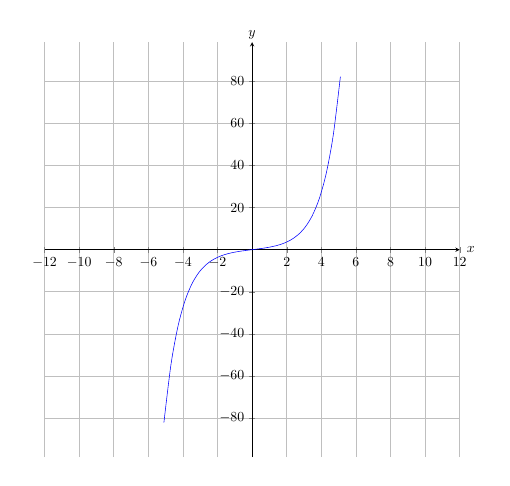
\begin{tikzpicture}[scale=.5]
		\begin{axis}[
			xmin=-10,xmax=10,
			restrict y to domain=-100:100,
			grid=both,width=\textwidth,height=\textwidth,
			axis lines=middle,
			xlabel=$x$,
			ylabel=$y$,
			enlarge x limits=0.1,
			enlarge y limits=0.1,
			x label style={at={(ticklabel* cs:1.00)}, inner sep=5pt, anchor=west},
			y label style={at={(ticklabel* cs:1.00)}, inner sep=2pt, anchor=south},
		]
			\addplot[color=blue,samples=50,smooth,domain=-10:10]{.5*(exp(x)-exp(-x))};
		\end{axis}
	\end{tikzpicture}
	\caption{双曲正弦函数\(\sinh\)的图形}
	\label{figure:函数.双曲正弦函数的图形}
\end{figure}

\begin{figure}[htb]
	\centering
	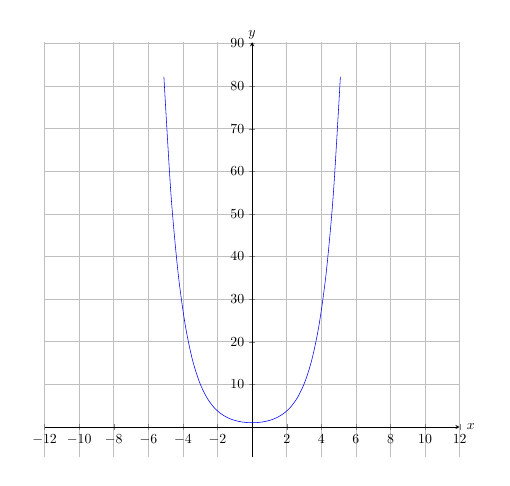
\begin{tikzpicture}[scale=.5]
		\begin{axis}[
			xmin=-10,xmax=10,
			restrict y to domain=-100:100,
			grid=both,width=\textwidth,height=\textwidth,
			axis lines=middle,
			xlabel=$x$,
			ylabel=$y$,
			enlarge x limits=0.1,
			enlarge y limits=0.1,
			x label style={at={(ticklabel* cs:1.00)}, inner sep=5pt, anchor=west},
			y label style={at={(ticklabel* cs:1.00)}, inner sep=2pt, anchor=south},
		]
			\addplot[color=blue,samples=50,smooth,domain=-10:10]{.5*(exp(x)+exp(-x))};
		\end{axis}
	\end{tikzpicture}
	\caption{双曲余弦函数\(\cosh\)的图形}
	\label{figure:函数.双曲余弦函数的图形}
\end{figure}

\begin{figure}[htb]
	\centering
	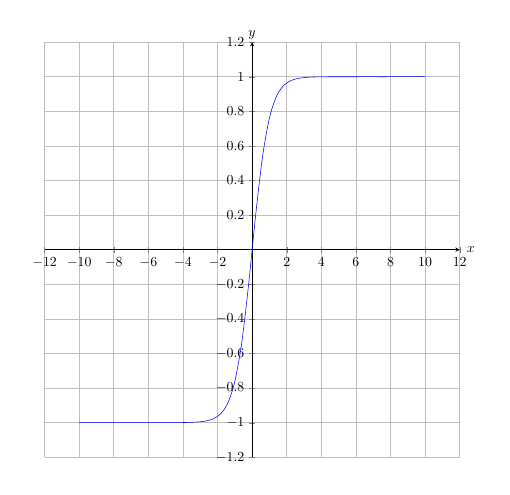
\begin{tikzpicture}[scale=.5]
		\begin{axis}[
			xmin=-10,xmax=10,
			restrict y to domain=-100:100,
			grid=both,width=\textwidth,height=\textwidth,
			axis lines=middle,
			xlabel=$x$,
			ylabel=$y$,
			enlarge x limits=0.1,
			enlarge y limits=0.1,
			x label style={at={(ticklabel* cs:1.00)}, inner sep=5pt, anchor=west},
			y label style={at={(ticklabel* cs:1.00)}, inner sep=2pt, anchor=south},
		]
			\addplot[color=blue,samples=50,smooth,domain=-10:10]{(exp(x)-exp(-x))/(exp(x)+exp(-x))};
		\end{axis}
	\end{tikzpicture}
	\caption{双曲正切函数\(\tanh\)的图形}
	\label{figure:函数.双曲正切函数的图形}
\end{figure}

\begin{figure}[htb]
	\centering
	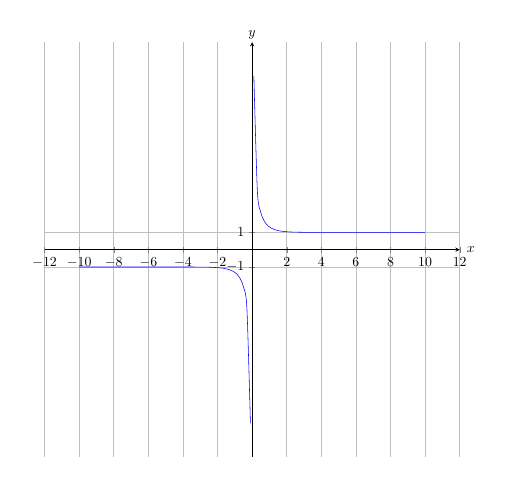
\begin{tikzpicture}[scale=.5]
		\begin{axis}[
			xmin=-10,xmax=10,
			ymin=-10,ymax=10,
			grid=both,width=\textwidth,height=\textwidth,
			axis lines=middle,
			xlabel=$x$,
			ylabel=$y$,
			enlarge x limits=0.1,
			enlarge y limits=0.1,
			x label style={at={(ticklabel* cs:1.00)}, inner sep=5pt, anchor=west},
			y label style={at={(ticklabel* cs:1.00)}, inner sep=2pt, anchor=south},
			ytick={-1,1},
		]
			\addplot[color=blue,samples=50,smooth,domain=-10:-.1]
				{(exp(x)+exp(-x))/(exp(x)-exp(-x))};
			\addplot[color=blue,samples=50,smooth,domain=.1:10]
				{(exp(x)+exp(-x))/(exp(x)-exp(-x))};
		\end{axis}
	\end{tikzpicture}
	\caption{双曲余切函数\(\coth\)的图形}
	\label{figure:函数.双曲余切函数的图形}
\end{figure}

\begin{figure}[htb]
	\centering
	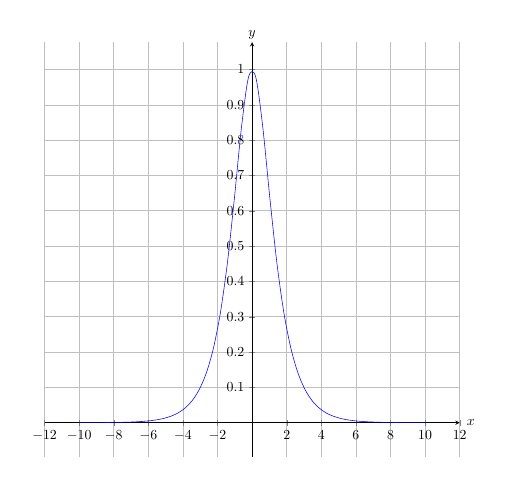
\begin{tikzpicture}[scale=.5]
		\begin{axis}[
			xmin=-10,xmax=10,
			restrict y to domain=-100:100,
			grid=both,width=\textwidth,height=\textwidth,
			axis lines=middle,
			xlabel=$x$,
			ylabel=$y$,
			enlarge x limits=0.1,
			enlarge y limits=0.1,
			x label style={at={(ticklabel* cs:1.00)}, inner sep=5pt, anchor=west},
			y label style={at={(ticklabel* cs:1.00)}, inner sep=2pt, anchor=south},
		]
			\addplot[color=blue,samples=50,smooth,domain=-10:10]{2/(exp(x)+exp(-x))};
		\end{axis}
	\end{tikzpicture}
	\caption{双曲正割函数\(\sech\)的图形}
\end{figure}

\begin{figure}[htb]
	\centering
	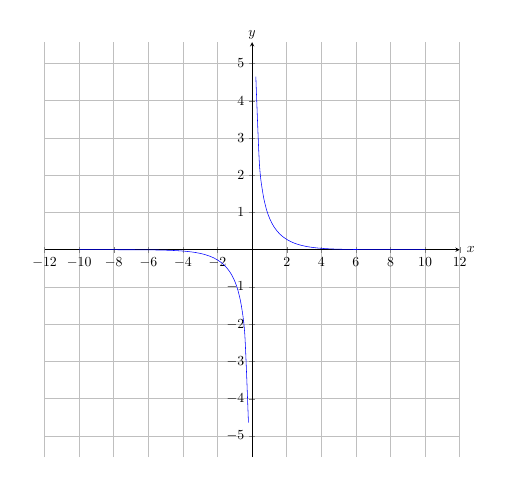
\begin{tikzpicture}[scale=.5]
		\begin{axis}[
			xmin=-10,xmax=10,
			restrict y to domain=-100:100,
			grid=both,width=\textwidth,height=\textwidth,
			axis lines=middle,
			xlabel=$x$,
			ylabel=$y$,
			enlarge x limits=0.1,
			enlarge y limits=0.1,
			x label style={at={(ticklabel* cs:1.00)}, inner sep=5pt, anchor=west},
			y label style={at={(ticklabel* cs:1.00)}, inner sep=2pt, anchor=south},
		]
			\addplot[color=blue,samples=50,smooth,domain=-10:-.01]{2/(exp(x)-exp(-x))};
			\addplot[color=blue,samples=50,smooth,domain=.01:10]{2/(exp(x)-exp(-x))};
		\end{axis}
	\end{tikzpicture}
	\caption{双曲余割函数\(\csch\)的图形}
\end{figure}

下面我们研究双曲函数的反函数.

首先讨论双曲正弦\(y=\sinh x\)的反函数.
由\(x=\sinh y\),有\[
	x=\frac{e^y-e^{-y}}{2}.
\]
令\(u=e^y\),则有\[
	u^2-2xu-1=0.
\]
这是一个关于\(u\)的一元二次方程,解得\[
	u=x\pm\sqrt{x^2+1}.
\]
因为\(u=e^y>0\),故上式根号前应取正号,即\[
	u=x+\sqrt{x^2+1}.
\]
又由\(y=\ln u\),故得反双曲正弦\[
	\arsinh x
	\defeq
	\ln(x+\sqrt{x^2+1}),
	\quad -\infty<x<+\infty.
\]

接下来讨论双曲余弦函数\(y=\cosh x\)的反函数.
由\(x=\cosh y\),有\[
	x=\frac{e^y+e^{-y}}{2},
\]
显然恒有\(x>0\).
由此得\(e^y=x\pm\sqrt{x^2-1}\ (x\geq1)\),
故\[
	y=\ln(x\pm\sqrt{x^2-1})
	\quad(x\geq1).
\]
可见,函数\[
	y=\ln(x+\sqrt{x^2-1})
	\quad(x\geq1)
\]是双曲余弦函数右支\(y=\cosh x\ (x\geq0)\)的反函数,
我们把它记作\(\arcosh x\),
即\[
	\arcosh x
	\defeq
	\ln(x + \sqrt{x^2 - 1}),
	\quad 1\leq x<+\infty.
\]
而函数\[
	y=\ln(x-\sqrt{x^2-1})
	\quad(x\geq1)
\]是双曲余弦函数左支\(y=\cosh x\ (x\leq0)\)的反函数.

易见\[
	\ln(x+\sqrt{x^2-1}) + \ln(x-\sqrt{x^2-1}) = 0
	\quad(x\geq1).
\]
%@Mathematica: FullSimplify[Log[x + Sqrt[x^2 - 1]] + Log[x - Sqrt[x^2 - 1]], Assumptions -> {x >= 1}]
%@credit: {cee35532-e299-4587-89a0-7b84e7454774}

然后讨论双曲正切函数\(\tanh\)的反函数.
由\[
	x = \tanh y
	= \frac{e^y-e^{-y}}{e^y+e^{-y}}
	= \frac{e^{2y}-1}{e^{2y}+1},
\]得\[
	(1-x) e^{2y} = 1+x,
\]
解得\(y = \frac12 \ln\frac{1+x}{1-x}\).
要使对数\(\ln\frac{1+x}{1-x}\)有意义,必有\((1+x)(1-x)>0\),
即\(x\in(-1,1)\).
于是反双曲正切函数可以定义为\[
	\artanh x
	\defeq
	\frac12 \ln\frac{1 + x}{1 - x},
	\quad -1<x<1.
\]

最后讨论双曲余切函数\(\coth\)的反函数.
由\[
	x = \coth y
	= \frac{e^y+e^{-y}}{e^y-e^{-y}}
	= \frac{e^{2y}+1}{e^{2y}-1},
\]得\[
	(x-1) e^{2y} = 1+x,
\]
解得\(y = \frac12 \ln\frac{x+1}{x-1}\).
要使对数\(\ln\frac{x+1}{x-1}\)有意义,必有\((x+1)(x-1)>0\),
即\(x\in(-\infty,-1)\cup(1,+\infty)\).
于是反双曲余切函数可以定义为\[
	\arcoth x
	\defeq
	\frac12 \ln\frac{x + 1}{x - 1},
	\quad -\infty<x<-1\lor1<x<+\infty.
\]

\begin{property}
双曲正弦\(\sinh\)是奇函数.
\end{property}

\begin{property}
双曲余弦\(\cosh\)是偶函数.
\end{property}

\begin{property}
\(\cosh x\)有下界:\[
	\cosh x \geq 1
\]
当且仅当\(x=0\)时,上式取等号.
\end{property}

\begin{theorem}
\begin{gather}
	\sinh(x \pm y) = \sinh x\cosh y \pm \cosh x\sinh y, \\
	\cosh(x \pm y) = \cosh x\cosh y \pm \sinh x\sinh y, \\
	\tanh(x + y) = \frac{\tanh x + \tanh y}{1 + \tanh x\tanh y}.
\end{gather}
\begin{proof}
根据双曲函数的定义有
\begin{align*}
	\sinh x\cosh y+\cosh x\sinh y
	&= \frac{e^x - e^{-x}}{2} \frac{e^y + e^{-y}}{2}
		+ \frac{e^x + e^{-x}}{2} \frac{e^y - e^{-y}}{2} \\
	&= \frac{1}{4} (e^x e^y + e^x e^{-y} - e^{-x} e^y - e^{-x} e^{-y} \\
	&\qquad+ e^x e^y - e^x e^{-y} + e^{-x} e^y - e^{-x} e^{-y}) \\
	&= \frac{1}{4} (2 e^x e^y - 2 e^{-x} e^{-y}) \\
	&= \frac12 (e^{x+y} - e^{-x-y}) = \sinh(x+y).
\end{align*}
\begin{align*}
	\cosh x\cosh y+\sinh x\sinh y
	&= \frac{e^x + e^{-1}}{2} \frac{e^y + e^{-y}}{2}
		+ \frac{e^x - e^{-x}}{2} \frac{e^y - e^{-y}}{2} \\
	&= \frac{1}{4} (e^x e^y + e^x e^{-y} + e^{-x} e^y + e^{-x} e^{-y} \\
	&\qquad+ e^x e^y - e^x e^{-y} - e^{-x} e^y + e^{-x} e^{-y}) \\
	&= \frac{1}{4} (2 e^x e^y + 2 e^{-x} e^{-y}) \\
	&= \frac12 (e^{x+y} + e^{-x-y}) = \cosh(x+y).
	\qedhere
\end{align*}
\end{proof}
\end{theorem}

\begin{theorem}
\begin{gather}
	\cosh^2x - \sinh^2x = 1, \\
	\sinh x + \cosh x = e^x, \\
	\cosh x - \sinh x = e^{-x}, \\
	1 - \tanh^2 x = \sech^2 x, \\
	\coth^2 x - 1 = \csch^2 x.
\end{gather}
\begin{proof}
根据双曲函数的定义有
\begin{align*}
	\cosh^2x-\sinh^2x
	&=\left(\frac{e^x + e^{-x}}{2}\right)^2-\left(\frac{e^x - e^{-x}}{2}\right)^2 \\
	&=\frac{e^{2x}+2+e^{-2x}}{4}-\frac{e^{2x}-2+e^{-2x}}{4}
	=1.
	\qedhere
\end{align*}
\end{proof}
\end{theorem}

\begin{theorem}
\begin{gather}
	\sinh2x = 2 \sinh x\cosh x, \\
	\cosh2x = \cosh^2x + \sinh^2x.
\end{gather}
\end{theorem}

\input{初等数学/函数/幂指函数}
\section{其他常见函数}
\subsection{单位阶跃函数}
\begin{definition}
函数\[
f(x) = \left\{ \begin{array}{cc}
0, & x < 0, \\
1, & x \geq 1
\end{array} \right.
\]称为\DefineConcept{单位阶跃函数}或\DefineConcept{赫维赛德阶跃函数}.
\end{definition}

\begin{figure}[ht]
	\centering
	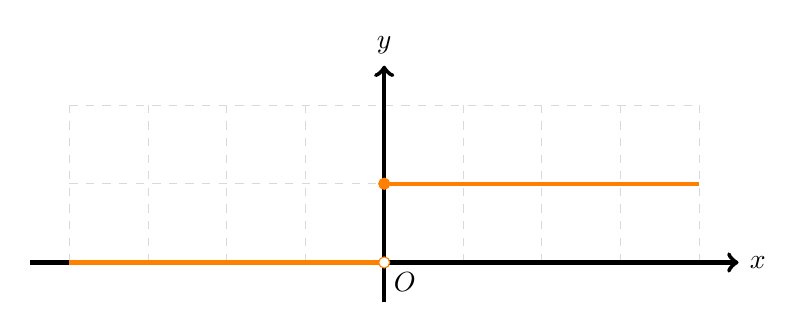
\begin{tikzpicture}
		\draw[help lines,color=gray!30,dashed](-4,0)grid(4,2);
		\draw[->,ultra thick](-4.5,0)--(4.5,0)node[right]{\(x\)};
		\draw[->,ultra thick](0,-.5)--(0,2.5)node[above]{\(y\)};
		\draw (0,0)node[below right]{\(O\)};
		\draw[orange,ultra thick](-4,0)--(0,0) (0,1)--(4,1);
		\draw[draw=orange,fill=orange](0,1)circle(2pt);
		\draw[draw=orange,fill=white](0,0)circle(2pt);
	\end{tikzpicture}
	\caption{单位阶跃函数的图形}
\end{figure}

\subsection{克罗内克\texorpdfstring{\(\delta\)}{\textdelta}函数}
\begin{definition}
%@see: https://mathworld.wolfram.com/KroneckerDelta.html
定义:\[
\delta_K(a,b)
\defeq \left\{ \begin{array}{cl}
	1, & a = b, \\
	0, & a \neq b.
\end{array} \right.
\]称其为\DefineConcept{克罗内克\(\delta\)函数}.
\end{definition}

\subsection{狄拉克\texorpdfstring{\(\delta\)}{\textdelta}函数}
\begin{definition}
%@see: https://functions.wolfram.com/GeneralizedFunctions/DiracDelta/02/
%@see: https://functions.wolfram.com/GeneralizedFunctions/DiracDelta2/02/
定义:\[
	\delta_D(x)
	\defeq \frac{1}{\pi}
		\lim_{\epsilon\to0}
		\frac{\epsilon}{x^2+\epsilon^2}
	\quad(x\in\mathbb{R}).
\]
称其为\DefineConcept{狄拉克\(\delta\)函数}.
\end{definition}

%@see: https://mathworld.wolfram.com/DeltaFunction.html

\section{隐函数}
\subsection{由参数方程确定的函数}
%@see: https://www.bilibili.com/video/BV1DNsoeAEii
\begin{example}
%@see: 《2023年全国硕士研究生入学统一考试(数学一)》一选择题/第3题
求解由参数方程\[
	\left\{ \begin{array}{l}
		x = 2t + \abs{t}, \\
		y = \abs{t} \sin t
	\end{array} \right.
\]确定的函数\(y = f(x)\).
\begin{solution}
当\(t\geq0\)时,\(x = 2t + t = 3t \geq 0\),\(y = t \sin t\).
当\(t<0\)时,\(x = 2t - t = t < 0\),\(y = -t \sin t\).
因此\[
	f(x) = \left\{ \begin{array}{cl}
		\frac{x}{3} \sin \frac{x}{3}, & x\geq0, \\
		-x \sin x, & x<0.
	\end{array} \right.
\]
\end{solution}
\end{example}
\begin{example}
求解由参数方程\[
	\left\{ \begin{array}{l}
		x = t \abs{t}, \\
		y = \abs{t} \sin t^2
	\end{array} \right.
\]确定的函数\(y = f(x)\).
\begin{solution}
当\(t\geq0\)时,\(x = t^2 \geq 0\),\(t = \sqrt{x}\),\(y = t \sin t^2\).
当\(t<0\)时,\(x = -t^2 < 0\),\(t = -\sqrt{-x}\),\(y = -t \sin t^2\).
因此\[
	f(x) = \left\{ \begin{array}{cl}
		\sqrt{x} \sin x, & x\geq0, \\
		-\sqrt{-x} \sin x, & x<0.
	\end{array} \right.
\]
\end{solution}
\end{example}

\section{抽象函数}
方程\[
	f(x+y) = f(x) + f(y) + c
\]确定的函数\(f\)称为直线型抽象函数,
其中\(c\)是与\(x\)、\(y\)无关的常数.

方程\[
	f(xy) = f(x) f(y)
\]确定的函数\(f\)称为幂函数型抽象函数.

方程\[
	f(x+y) = f(x) f(y)
\]或\[
	f(xy) = [f(x)]^y
\]确定的函数\(f\)称为指数函数型抽象函数.

方程\[
	f(xy) = f(x) + f(y)
\]或\[
	f\left(\frac{x}{y}\right) = f(x) - f(y)
\]确定的函数\(f\)称为对数函数型抽象函数.

方程\[
	f(x) + f(y) = 2 f\left(\frac{x+y}{2}\right) f\left(\frac{x-y}{2}\right)
\]或\[
	f(x+y) = \frac{f(x) + f(y)}{1 - f(x) f(y)}
\]确定的函数\(f\)称为三角函数型抽象函数.

\section{初等函数}
\begin{definition}
%@see: 《数学分析教程(第3版 上册)》(史济怀) P94
\emph{常函数}、\emph{幂函数}、\emph{指数函数}、\emph{对数函数}、\emph{三角函数}、\emph{反三角函数}这六类函数统称为\DefineConcept{基本初等函数}.
由常数和基本初等函数经过有限次四则运算和有限次函数复合步骤所构成并可用一个式子表示的函数,称为\DefineConcept{初等函数}.
\end{definition}


\chapter{数列}
\section{数列的概念}
\begin{definition}\label{definition:数列.数列的定义}
一般地,如果\(D \subseteq \mathbb{Z}\),
那么把映射\[
    f\colon D\to\mathbb{R}, n \mapsto a_n
\]称为一个\DefineConcept{数列}(sequence,progression),
记作\(\{a_n\}\),即\(\{a_n\} \defeq f\).

数列中的每一个数(例如\(\AutoTuple{a}{0}\))叫做数列的\DefineConcept{项}(term).

把表示第\(n\)个数\(a_n\)的公式称为“数列\(\{a_n\}\)的\DefineConcept{一般项}”.
\end{definition}

应该指出,如果我们说“数列\(\{x_n\}\)在数集\(X\)内”或\(\{x_n\} \subseteq X\),
我们指的是:把数列\(\{x_n\}\)看作一个映射\(f\)时,
这个映射的值域\(\ran f\)是\(X\)的子集,即\(\ran f \subseteq X\).

\begin{definition}
如果数列\(\{x_n\}\)满足条件\[
	x_n \leq x_{n+1}, \quad n=1,2,\dotsc,
\]
就称“数列\(\{x_n\}\)是\DefineConcept{单调增加的}”.

如果数列\(\{x_n\}\)满足条件\[
	x_n \geq x_{n+1}, \quad n=1,2,\dotsc,
\]
就称“数列\(\{x_n\}\)是\DefineConcept{单调减少的}”.

单调增加数列和单调减少数列统称为\DefineConcept{单调数列}.
如果数列\(\{x_n\}\)是单调数列,则称“\(\{x_n\}\)具有单调性”.
\end{definition}

\begin{definition}
如果数列\(\{x_n\}\)满足\[
	(\forall n \geq N)[x_n \leq x_{n+1}],
\]
则称“数列\(\{x_n\}\)从第\(N\)项起单调增加”.

如果数列\(\{x_n\}\)满足\[
	(\forall n \geq N)[x_n \geq x_{n+1}],
\]
则称“数列\(\{x_n\}\)从第\(N\)项起单调减少”.
\end{definition}

\begin{proposition}
设数列\(\{x_n\}\)满足\[
	(x_{n+1}-x_n)(x_n-x_{n-1})>0
	\quad(n=2,3,\dotsc),
\]
则\(\{x_n\}\)具有单调性.
\end{proposition}

\begin{definition}[数列的有界性]
设数列\(\{x_n\}\).

如果\[
	(\exists M>0)
	(\forall n\in\mathbb{N})
	[\abs{x_n} \leq M],
\]
那么称“数列\(\{x_n\}\)是\DefineConcept{有界的}”.

如果这样的正数\(M\)不存在,即\[
	(\forall M>0)
	(\exists n\in\mathbb{N})
	[\abs{x_n} > M],
\]
那么称“数列\(\{x_n\}\)是\DefineConcept{无界的}”.
\end{definition}

例如,数列\(x_n = \frac{n}{n+1}\ (n=1,2,\dotsc)\)是有界的,
因为可取\(M=1\),而使\[
	\abs{\frac{n}{n+1}} \leq 1
\]对于一切正整数\(n\)都成立.

数列\(x_n = 2^n\ (n=1,2,\dotsc)\)是无界的,因为当\(n\)无限增加时,\(2^n\)可超过任何正数.

\begin{definition}
%@see: 《数学分析(第二版 上册)》(陈纪修) P62 定义2.4.2
设\(\{a_n\}\)是数列,
我们把\(\{a_n\}\)的子集称为“\(\{a_n\}\)的\DefineConcept{子列}”.
\end{definition}
我们常把数列\(\{a_n\}\)的子列记作\(\{a_{n_k}\}\),
这里下标\(n_k\)表示子列中的第\(k\)项恰好是原数列\(\{a_n\}\)中的第\(n_k\)项.
应该注意到,由于子列下标\(n_k\)是严格单调增加的,
所以\[
	(\forall k\in\mathbb{N}^+)
	[n_k \geq k],
\]
且\[
	(\forall i,j\in\mathbb{N}^+)
	[i \geq j \implies n_i \geq n_j].
\]

\section{数列的连加与连乘}
\subsection{数列的连加}
\begin{definition}[连加]
定义\DefineConcept{连续求和}:\[
	\sum_{i=m}^n a_i
	\defeq
	a_m + a_{m+1} + \dotsb + a_{n-1} + a_n
	\quad(m \leq n),
\]其中符号\(\sum\)称作\DefineConcept{连加号},
符号\(i\)称为\DefineConcept{求和指标}(index of summation),
整数\(m\)称为\DefineConcept{求和下限}(lower bound),
整数\(n\)称为\DefineConcept{求和上限}(upper bound),
符号\(a_i\)称为\DefineConcept{求和通项}(summand).
\end{definition}

\begin{figure}[ht]
	\centering
	\begin{tikzpicture}
		\draw(0,0)node{$\sum_{
			{\textcolor{red}i}
			=
			{\textcolor{blue}m}
		}^{\textcolor{yellow-green}n} x_i$};
		\draw(-.2,1)node{\textcolor{yellow-green}{求和上限}};
		\draw(-1.5,-.5)node{\textcolor{red}{求和指标}};
		\draw(1.1,-.5)node{\textcolor{blue}{求和下限}};
	\end{tikzpicture}
	\caption{}
\end{figure}

有时候也把\(\sum_{i=m}^n\)%
写作\(\sum_{m \leq i \leq n}\).

使用双重连加号求和时,如果两个求和指标独立取值,则连加号\(\sum\)的顺序可以交换.

在不引起误解的情况下,可以省略不写求和指标,
例如用\(\sum a_n\)表示\(\sum_{k=1}^n a_k\).

\subsection{数列的连乘}
\begin{definition}[连乘]
定义\DefineConcept{连续求积}:\[
\prod_{i=m}^n a_i
\defeq
a_m \times a_{m+1} \times \dotsb \times a_{n-1} \times a_n
\quad(m \leq n),
\]其中符号\(\prod\)称作\DefineConcept{连乘号},整数\(i\)称为\DefineConcept{求积指标}.
\end{definition}

同样地,有时候也把\(\prod_{i=m}^n\)%
写作\(\prod_{m \leq i \leq n}\).

\begin{definition}\label{definition:数列.阶乘的定义}
给定一个正整数\(n\),
称所有小于或等于\(n\)的正整数的积为“\(n\)的\DefineConcept{阶乘}(factorial)”,
记作\(n!\),即
\begin{equation}
n!
\defeq
\prod_{k=1}^n k
=
n \times (n-1) \times (n-2) \times \dotsm \times 2 \times 1.
\end{equation}
特别地,规定\(0! = 1\).
\end{definition}

\begin{table}[ht]
	\centering
	\begin{subtable}[ht]{.3\textwidth}
		\centering
		\begin{tblr}{rcr}
			\hline
			0! & = & 1 \\
			1! & = & 1 \\
			2! & = & 2 \\
			3! & = & 6 \\
			4! & = & 24 \\
			5! & = & 120 \\
			6! & = & 720 \\
			7! & = & 5~040 \\
			8! & = & 40~320 \\
			9! & = & 362~880 \\
			\hline
		\end{tblr}
		\caption{}
	\end{subtable}~\begin{subtable}[ht]{.6\textwidth}
		\centering
		\begin{tblr}{rcr|rcr}
			\hline
			0!! & = & 1 & 1!! & = & 1 \\
			2!! & = & 2 & 3!! & = & 3 \\
			4!! & = & 8 & 5!! & = & 15 \\
			6!! & = & 48 & 7!! & = & 105 \\
			8!! & = & 384 & 9!! & = & 945 \\
			10!! & = & 3~840 & 11!! & = & 10~395 \\
			12!! & = & 46~080 & 13!! & = & 135~135 \\
			14!! & = & 645~120 & 15!! & = & 2~027~025 \\
			16!! & = & 10~321~920 & 17!! & = & 34~459~425 \\
			18!! & = & 185~794~560 & 19!! & = & 654~729~075 \\
			\hline
		\end{tblr}
		\caption{}
	\end{subtable}
	\caption{}
%@Mathematica: Table[{n, n!}, {n, 0, 9}]
%@Mathematica: Table[{n, n!!}, {n, 0, 20, 2}]
%@Mathematica: Table[{n, n!!}, {n, 1, 20, 2}]
\end{table}

\begin{definition}
给定一个正整数\(n\),
称小于或等于\(n\)且与之同奇偶的所有正整数的积为“\(n\)的\DefineConcept{双阶乘}”,
记作\(n!!\),即
\begin{equation}
	n!!
	\defeq
	\begin{cases}
		n \times (n-2) \times (n-4) \times \dotsm \times 3 \times 1, & n\text{是奇数}, \\
		n \times (n-2) \times (n-4) \times \dotsm \times 4 \times 2, & n\text{是偶数}.
	\end{cases}
\end{equation}
特别地,规定\(0!! = 1\).
\end{definition}

需要注意的是,通常来说双阶乘\(n!!\)并不等于“阶乘的阶乘”\((n!)!\),
实际上,\(3!! = 3\)而\((3!)! = 6! = 720\).

\section{等差数列}
一般地,如果一个数列从第2项起,每一项与它的前一项的差等于同一个常数,
这个数列就叫做\DefineConcept{等差数列}(arithmetical progression),
这个常数叫做等差数列的\DefineConcept{公差}(common difference).

如果数列\(\{a_n\}\)是等差数列,它的公差是\(d\),那么\begin{align*}
    a_2 &= a_1 + d, \\
    a_3 &= a_2 + d = (a_1 + d) + d = a_1 + 2d, \\
    a_4 &= a_3 + d = (a_1 + 2d) + d = a_1 + d3.
\end{align*}
以此类推,可知等差数列\(\{a_n\}\)的\DefineConcept{通项公式}是\begin{equation}
    a_n = a_1 + (n-1) d.
\end{equation}

将等差数列中任意两项\[
    a_m = a_1 + (m-1) d
    \quad\text{与}\quad
    a_n = a_1 + (n-1) d
\]相减,得到\[
    a_m - a_n = (m-n) d.
\]
由此我们也可得到%
等差数列的\DefineConcept{递推公式}:\begin{equation}
    a_{n+1} - a_n = d.
\end{equation}

\begin{property}[等差数列求和]
设数列\(\{a_n\}\)为等差数列,它的通项公式为\[
    a_n = a_1 + (n-1) d,
\]
那么它的前\(n\)项和为\begin{equation}\label{equation:数列.等差数列的前n项和1}
    S_n = \frac{n(a_1 + a_n)}{2},
\end{equation}
或\begin{equation}\label{equation:数列.等差数列的前n项和2}
    S_n = n a_1 + \frac{n(n-1)}{2} d.
\end{equation}
\begin{proof}
由\[
    S_n = a_1 + (a_1 + d) + \dotsb + [a_1 + (n-2)d] + [a_1 + (n-1)d],
\]\[
    S_n = [a_n - (n-1)d] + [a_n - (n-2)d] + \dotsb + (a_n - d) + a_n,
\]相加得\[
    2 S_n = n(a_1 + a_n),
\]最终可得\[
    S_n = \frac{n(a_1 + a_n)}{2} = n a_1 + \frac{n(n-1)}{2} d.
    \qedhere
\]
\end{proof}
\end{property}

根据\hyperref[equation:数列.等差数列的前n项和1]{等差数列的前\(n\)项和公式},立即有如下结论:
\begin{equation}
    \sum_{k=1}^n k = \frac{1}{2} n(n+1).
\end{equation}

\begin{property}
设数列\(\{a_n\}\)是以\(d\)为公差的等差数列,
\(b\)是常数,
则\(\{b + a_n\}\)也是以\(d\)为公差的等差数列.
\end{property}

\begin{property}
设数列\(\{a_n\}\)是以\(d\)为公差的等差数列,
\(b\)是常数,
则\(\{b \cdot a_n\}\)是以\(b d\)为公差的等差数列.
\end{property}

\begin{example}
设\(\{a_n\}\)是等差数列.
证明:如果正整数\(m,n,p,q\)满足\(m+n=p+q\),
则\[
	a_m+a_n=a_p+a_q.
\]
\begin{proof}
设\(\{a_n\}\)的公差是\(d\),
则\(a_m-a_p = (m-p)d\).
由\(m+n=p+q\)
移项得\(m-p=q-n\),
于是\(a_m-a_p = a_q-a_n\),
因此\(a_m+a_n=a_p+a_q\).
\end{proof}
\end{example}

\begin{example}
设\(\{a_n\}\)是公差为\(d\)的等差数列.
证明:\(S_k,S_{2k}-S_k,S_{3k}-S_{2k},\dotsc\)成为等差数列,
它的公差为\(k^2 d\).
\begin{proof}
既然\(S_n = n a_1 + \frac12 n(n-1) d\ (n=1,2,\dotsc)\),
那么\begin{align*}
	&\hspace{-20pt}
	(S_{2k}-S_k) - S_k
	= S_{2k} - 2 S_k \\
	&= 2k a_1 + \frac12 (2k)(2k-1) d
	- 2 k a_1 - k(k-1) d \\
	&= k^2 d, \\
	&\hspace{-20pt}
	[S_{(m+1)k}-S_{mk}] - [S_{mk}-S_{(m-1)k}]
	= S_{(m+1)k} - 2 S_{mk} + S_{(m-1)k} \\
	&= (mk+k) a_1 + \frac12 (mk+k)(mk+k-1) d \\
	&\hspace{20pt}
	- 2 mk a_1 - mk (mk-1) d \\
	&\hspace{20pt}
	+ (mk-k) a_1 + \frac12 (mk-k)(mk-k-1) d \\
	&= k^2 d.
	\qedhere
\end{align*}
\end{proof}
\end{example}

\begin{example}
设数列\(\{a_n\}\)的前\(n\)项和为\(S_n\).
证明:\(\left\{\frac{S_n}{n}\right\}\)是等差数列.
\begin{proof}
设\(\{a_n\}\)的公差是\(d\).
因为\(S_n=\frac{n}2(a_1+a_n)\),
所以\(\frac{S_n}{n}=\frac12(a_1+a_n)\),
从而\[
	\frac{S_{n+1}}{n+1}-\frac{S_n}{n}
	= \frac12(a_1+a_{n+1})-\frac12(a_1+a_n)
	= \frac12(a_{n+1}-a_n)
	= \frac{d}2.
\]
这就说明\(\left\{\frac{S_n}{n}\right\}\)是公差为\(\frac{d}2\)的等差数列.
\end{proof}
\end{example}

\begin{example}
设数列\(\{a_n\}\)的前\(n\)项和\(S_n = a_1 + a_2 + \dotsb + a_n\)满足\[
	S_n = A n^2 + B n + C,
\]
其中\(A,B,C\)是常数.
证明:\begin{itemize}
	\item 若\(C = 0\),则\(\{a_n\}\)是等差数列.
	\item 若\(C \neq 0\),则\(\{a_n\}\)从第二项起成为等差数列.
\end{itemize}
\begin{proof}
首先\[
	a_1 = S_1 = A + B + C, \qquad
	a_n = 2A n + (B-A), \quad n=2,3,\dotsc,
\]
于是\[
	a_2 - a_1
	= 2A - C, \qquad
	a_{n+1} - a_n
	= 2A, \quad n=2,3,\dotsc.
\]
因此\[
	\text{\(\{a_n\}\)是等差数列}
	\iff
	a_2 - a_1 = a_3 - a_2
	\iff
	2A - C = 2A
	\iff
	C = 0.
	\qedhere
\]
\end{proof}
\end{example}

\begin{example}
设\(\{a_n\},\{b_n\}\)都是等差数列.
证明:\(\{a_{b_n}\}\)也是等差数列.
\begin{proof}
设\(\{a_n\},\{b_n\}\)的公差分别为\(d_1,d_2\),
则\[
	a_{b_{n+1}}-a_{b_n}
	=(b_{n+1}-b_n)d_1
	=d_1 d_2,
\]
这就说明\(\{a_{b_n}\}\)是公差为\(d_1 d_2\)的等差数列.
\end{proof}
\end{example}

\begin{example}
设\(\{a_n\},\{b_n\}\)都是等差数列.
证明:\(\{p a_n + q b_n\}\)也是等差数列,其中\(p,q\)是常数.
\begin{proof}
设\(\{a_n\},\{b_n\}\)的公差分别为\(d_1,d_2\),
则\[
	(p a_{n+1} + q b_{n+1})
	- (p a_n + q b_n)
	= p (a_{n+1} - a_n)
	+ q (b_{n+1} - b_n)
	= p d_1 + q d_2,
\]
这就说明\(\{a_{b_n}\}\)是公差为\(p d_1 + q d_2\)的等差数列.
\end{proof}
\end{example}

\section{平方数列}
如果数列\(\{a_n\}\)的通项公式是\[
a_n = n^2,
\]那么称其为\DefineConcept{平方数列}.

由立方差公式可知
\[\begin{aligned}
n^3 - (n-1)^3
&= [n - (n-1)] \cdot [n^2 + n(n-1) + (n-1)^2] \\
&= 2n^2 + (n-1)^2 - n.
\end{aligned}\]于是将\[
\begin{array}{l}
2^3 - 1^3 = 2\times2^2+1^2-2, \\
3^3 - 2^3 = 2\times3^2+2^2-3, \\
\hdotsfor{1} \\
n^3 - (n-1)^3 = 2n^2 + (n-1)^2 - n,
\end{array}
\]相加便得\[\begin{aligned}
n^3 - 1^3
&= 2(2^2+3^2+\dotsb+n^2) + [1^2+2^2+\dotsb+(n-1)^2] - (2+3+\dotsb+n) \\
&= 2\left(\sum_{k=1}^n k^2 - 1\right)
    + \left(\sum_{k=1}^n k^2 - n^2\right)
    - \left(\sum_{k=1}^n k - 1\right) \\
&= 3\sum_{k=1}^n k^2 - 2 - n^2 - \frac{n(n+1)}{2} + 1 \\
&= 3\sum_{k=1}^n k^2 - \frac{3}{2} n^2 - \frac{1}{2} n - 1,
\end{aligned}\]
移项,得\[
3 \sum_{k=1}^n k^2
= n^3 + \frac{3}{2} n^2 + \frac{1}{2} n
= \frac{1}{2} n (n+1) (2n+1).
\]
因此,平方数列的前\(n\)项之和为
\begin{equation}
	\sum_{k=1}^n a_n
	= \sum_{k=1}^n k^2
	= \frac{1}{6} n(n+1)(2n+1).
\end{equation}

\begin{example}
求在正方形底上排成完整棱锥体的小球个数.
\begin{solution}
设底部每边有\(n\)个小球,则最底层小球的个数为\(n^2\)个;
从下往上数,第二层有\((n-1)^2\)个小球,
第三层有\((n-2)^2\)个小球,
以此类推,直至顶层只有一个小球.
因此,棱锥体的小球个数为\[
    S = n^2+(n-1)^2+(n-2)^2+\dotsb+1
    = \frac{n(n+1)(2n+1)}{6}.
\]
\end{solution}
\end{example}

\begin{example}
求在等边三角形底上排成完整棱锥体的小球个数.
\begin{solution}
设底部每边有\(n\)个小球,则最底层小球的个数为\[
    n+(n-1)+(n-2)+\dotsb+1
    = \frac{n(n+1)}{2}
    = \frac{1}{2}(n^2+n).
\]
在上式中以\((n-1),(n-2),\dotsc\)替代\(n\),
就得到了从下往上数从第二层开始直至最顶层的小球个数.
因此,棱锥体的小球个数为\[
    S = \frac{1}{2} (\sum n^2 + \sum n)
    = \frac{n(n+1)(n+2)}{6}.
\]
\end{solution}
\end{example}

\section{立方数列}
如果数列\(\{a_n\}\)的通项公式是\[
a_n = n^3,
\]那么称其为\DefineConcept{立方数列}.

由平方差公式可知
\[\begin{aligned}
n^4 - (n-1)^4
&= [n^2 - (n-1)^2] [n^2 + (n-1)^2] \\
&= [n - (n-1)] [n + (n-1)] [n^2 + (n-1)^2] \\
&= (2n-1) (2n^2 - 2n + 1) \\
&= 4n^3 - 6n^2 + 4n - 1.
\end{aligned}\]
于是\[
\sum_{k=1}^n [k^4 - (k-1)^4]
= \sum_{k=1}^n (4k^3 - 6k^2 + 4k - 1),
\]即\[\begin{aligned}
n^4
&= 4 \sum_{k=1}^n k^3 - 6 \sum_{k=1}^n k^2 + 4 \sum_{k=1}^n k - n \\
&= 4 \sum_{k=1}^n k^3 - n(n+1)(2n+1) + 2n(n+1) - n,
\end{aligned}\]
移项,得\[
4 \sum_{k=1}^n k^3
= n^4 + n(n+1)(2n+1) - 2n(n+1) + n
= n^4 + 2n^3 + n^2
= n^2(n+1)^2.
\]
因此,立方数列的前\(n\)项之和为
\begin{equation}
\sum_{k=1}^n a_n
= \sum_{k=1}^n k^3
= \left[\frac{n(n+1)}{2}\right]^2.
\end{equation}

\section{等比数列}
\begin{definition}
如果数列\(\{a_n\}\)满足\[
	a_n = a q^{n-1} \quad(a\neq0,q\neq1),
\]
则称该数列为\DefineConcept{等比数列}
或\DefineConcept{几何数列}(geometrical progression),
其中\(q\)称作\DefineConcept{公比}.

等比数列的递推公式为\(\frac{a_n}{a_{n-1}} = q\ (n \geq 2)\).
\end{definition}

将等比数列中任意两项\[
    a_m = a_1 q^{m-1}
    \quad\text{与}\quad
    a_n = a_1 q^{n-1}
\]相除,
得到\[
    \frac{a_m}{a_n} = q^{m-n}.
\]
由此我们也可得到等比数列的\DefineConcept{递推公式}:
\begin{equation}
	a_{n+1} = a_n q.
\end{equation}

\begin{property}[等比数列求和]\label{theorem:等比数列.前n项和}
设数列\(\{a_n\}\)是等比数列,
\(a_n = a q^{n-1}\ (n=1,2,\dotsc)\),
则有\begin{equation}
	\sum_{i=1}^n a_i
	= \left\{ \begin{array}{cl}
		\frac{a (q^n-1)}{q-1}, & q \neq 1, \\
		na, & q = 1.
	\end{array} \right.
\end{equation}
\begin{proof}
记\(S_n = \sum_{k=1}^n a_k
= a + aq + aq^2 + \dotsb + aq^{n-1}\),
于是\[
	S_{n+1} - S_n = aq^n.
	\eqno(1)
\]

当\(q = 1\)时,显然有\(S_n = na\).

当\(q \neq 1\)时,有\[
	q S_n
	= aq+aq^2+aq^3+\dotsb+aq^n,
	\eqno(2)
\]\[
	S_{n+1}
	= a+aq+aq^2+\dotsb+aq^{n-1}+aq^n,
	\eqno(3)
\]
用(3)式减去(2)式便得\[
	S_{n+1} - q S_n
	= a.
	\eqno(4)
\]
联立(1)(4)两式,得到关于\(S_n,S_{n+1}\)的二元一次方程组,
解得\[
	S_n = \frac{
		\begin{vmatrix}
			1 & a \\
			1 & a q^n
		\end{vmatrix}
	}{
		\begin{vmatrix}
			1 & -q \\
			1 & -1
		\end{vmatrix}
	}
	= \frac{a(q^n - 1)}{q-1}.
	\qedhere
\]
\end{proof}
\end{property}

\begin{property}
设数列\(\{a_n\}\)是以\(d\)为公差的等差数列,
\(b\)是非零常数,
则\(\{b^{a_n}\}\)是等比数列.
\begin{proof}
易见\[
	\frac{b^{a_{n+1}}}{b^{a_n}}
	= b^{a_{n+1}-a_n}
	= b^d,
\]
这就说明\(\{b^{a_n}\}\)是以\(b^d\)为公比的等比数列.
\end{proof}
\end{property}

\begin{example}
设\(\{a_n\}\)是等比数列.
证明:如果正整数\(m,n,p,q\)满足\(m+n=p+q\),
则\[
	a_m \cdot a_n = a_p \cdot a_q.
\]
\begin{proof}
设\(\{a_n\}\)的公比是\(q\),
则\(a_m / a_p = q^{m-p}\).
由\(m+n=p+q\)
移项得\(m-p=q-n\),
于是\(a_m / a_p = a_q / a_n\),
因此\(a_m \cdot a_n=a_p \cdot a_q\).
\end{proof}
\end{example}

\begin{property}
设数列\(\{a_n\}\)为等比数列,\(b\)为常数,则:
\begin{itemize}
    \item \(\{b \cdot a_n\}\)为等比数列,它的公比与\(\{a_n\}\)的一样;
    \item \(\{b / a_n\}\)为等比数列,它的公比是\(\{a_n\}\)的公比的倒数;
    \item \(\{\log_b a_n\}\)为等差数列.
\end{itemize}
\end{property}

\begin{example}
求级数\[
    a,(a+d)r,(a+2d)r^2,(a+3d)r^3,\dotsc
\]的前\(n\)项之和.
\begin{solution}
设所求级数的前\(n\)项之和为\[
    S_n = \sum_{k=0}^{n-1} (a+kd) r^k.
    \eqno(1)
\]
那么\[
    r S_n = \sum_{k=0}^{n-1} (a+kd) r^{k+1}.
    \eqno(2)
\]
将(1)式与(2)式相减,得\begin{align*}
    S_n(1-r) &= a + (dr + dr^2 + \dotsb + dr^{n-1}) - [a+(n-1)d] r^n \\
    &= a + \frac{dr(1-r^{n-1})}{1-r} - [a+(n-1)d] r^n.
\end{align*}
于是\[
    S_n = \frac{a}{1-r} + \frac{dr(1-r^{n-1})}{(1-r)^2} - \frac{[a+(n-1)d] r^n}{1-r}.
\]
\end{solution}
\end{example}

\section{调和数列}
若数列\(\{a_n\}\)每相邻三项满足\[
    \frac{a_{n+1}}{a_{n-1}}
    = \frac{a_{n+1}-a_n}{a_n-a_{n-1}},
\]
则称其为\DefineConcept{调和数列}(harmonical progression)\footnote{%
人们对调和数列有兴趣的主要原因是它在几何学与声学中有其重要性.
调和数列的若干项求和无一般公式可循.
通常来说,涉及调和数列的问题的解法都是将它的各项倒转,再利用对应的等差数列的性质.
};
称\(a_n\)为“\(a_{n-1}\)和\(a_{n+1}\)的\DefineConcept{调和中项}或\DefineConcept{调和平均数}”.

\begin{property}\label{theorem:数列.调和数列的性质}
调和数列\(\{a_n\}\)各项的倒数组成的数列\(\{1/a_n\}\)是等差数列.
\begin{proof}
根据调和数列的定义可知,\[
    \frac{a_{n+1}}{a_{n-1}}
    = \frac{a_{n+1}-a_n}{a_n-a_{n-1}},
\]整理得\[
    a_{n+1} (a_n - a_{n-1})
    = a_{n-1} (a_{n+1} - a_n),
\]再同除以\((a_{n+1} \cdot a_n \cdot a_{n-1})\),得\[
    \frac{1}{a_{n-1}} - \frac{1}{a_n}
    = \frac{1}{a_n} - \frac{1}{a_{n+1}}.
    \qedhere
\]
\end{proof}
\end{property}

\begin{example}
求\(a\)与\(b\)的调和平均数.
\begin{solution}
设\(a\)与\(b\)的调和平均数为\(h\).
由\cref{theorem:数列.调和数列的性质} 有\[
    \frac{1}{h} - \frac{1}{a}
    = \frac{1}{b} - \frac{1}{h},
\]\[
    \frac{2}{h} = \frac{1}{a} + \frac{1}{b}
    = \frac{a+b}{ab},
\]\[
    h = \frac{2ab}{a+b}.
\]
\end{solution}
\end{example}

我们知道,两个数\(x\)与\(y\)的算术平均数、几何平均数、调和平均数分别为\[
    A = \frac{x+y}{2}, \qquad
    G = \sqrt{xy}, \qquad
    H = \frac{2xy}{x+y}.
\]
由于\[
    A \cdot H = \frac{x+y}{2} \cdot \frac{2xy}{x+y}
    = ab = G^2,
\]
所以\(G\)又是\(A\)与\(H\)的几何平均数.
我们还注意到,当\(x,y>0\)且\(x \neq y\)时,\[
    A - G = \frac{x+y}{2} - \sqrt{xy}
    = \frac{x+y-2\sqrt{xy}}{2}
    = \left(\frac{\sqrt{x}-\sqrt{y}}{\sqrt{2}}\right)^2
    > 0,
\]
因此我们可以说:
两个正数的算术平均数总大于它们的几何平均数,即\(A > G\).
再考虑到\(G^2 = A H\),\(G\)是介于\(A\)与\(H\)之间的,于是必有\(G > H\).
综上所述,两个正数的算术平均数、几何平均数、调和平均数的大小依次递减,即\(A > G > H\).

\section{斐波那契数列}
如果数列\(\{a_n\}\)满足\(a_1=a_2=1\),且\[
a_n = a_{n-1} + a_{n-2} \quad(n\geq3),
\]则称该数列为\DefineConcept{斐波那契数列}.

\section{已知递推公式求解通项公式的方法}
\subsection{\texorpdfstring{形如\(a_{n+2}=p a_{n+1} + q a_n\ (q\neq0)\)的递推公式}{第一类递推公式}}
对于形如\(a_{n+2}=p a_{n+1} + q a_n\ (q\neq0)\)的递推公式,我们可以令\[
\vb{X}_n = \begin{bmatrix}
a_{n+1} \\
a_n
\end{bmatrix},
\qquad
\vb{A} = \begin{bmatrix}
p & q \\
1 & 0
\end{bmatrix},
\]则\(\vb{X}_{n+1} = \vb{A} \vb{X}_n\),从而\(\vb{X}_n = \vb{A}^{n-1} \vb{X}_1\).
这样就可以求出通项公式.

现在我们来求\(\vb{A}\)的幂.
此时\(\vb{A}\)的特征多项式为\[
f(x) = \begin{vmatrix}
x-p & -q \\
-1 & x
\end{vmatrix} = x^2 - px - q,
\]我们也称这个多项式为递推公式的特征方程.

假设我们求得该方程的两个复根为\(\alpha,\beta\),则由韦达定理可知\(p=\alpha+\beta, q=-\alpha\beta\).
注意到\[
\left\{ \begin{array}{l}
a_{n+2} - \alpha a_{n+1} = \beta(a_{n+1}-\alpha a_n), \\
a_{n+2} - \beta a_{n+1} = \alpha(a_{n+1}-\beta a_n)
\end{array} \right.,
\]从而\[
\left\{ \begin{array}{l}
a_{n+1} - \alpha a_n = \beta^{n-1} (a_2 - \alpha a_1), \\
a_{n+1} - \beta a_n = \alpha^{n-1} (a_2 - \beta a_1)
\end{array} \right.,
\]

若\(\alpha\neq\beta\),解关于\(a_{n+1},a_n\)的线性方程组可得\[
a_n = \frac{\beta^{n-1} (a_2 - \alpha a_1) - a^{n-1} (a_2 - \beta a_1)}{\beta-\alpha};
\]
若\(\alpha=\beta\),则\(\alpha=\beta\neq0\),从而\(a_{n+1} = \alpha a_n = \alpha^{n-1} (a_2 - \alpha a_1)\),进而\[
\frac{a_{n+1}}{\alpha^{n+1}} - \frac{a_n}{\alpha^n} = \frac{1}{\alpha^2}(a_2-\alpha a_1),
\]最后得到\[
a_n = (2-n)\alpha^{n-1} a_1 + (n-1) \alpha^{n-2} a_2.
\]

利用上述结论可以求出斐波那契数列的通项公式为\[
a_n = \frac{1}{\sqrt{5}} \left[
\left(\frac{1+\sqrt{5}}{2}\right)^n
-\left(\frac{1-\sqrt{5}}{2}\right)^n
\right].
\]

\subsection{\texorpdfstring{形如\(a_{n+1} = \frac{a a_n + b}{c a_n + d}\ (ad-bc\neq0)\)的递推公式}{第二类递推公式}}
对于形如\(a_{n+1} = \frac{a a_n + b}{c a_n + d}\ (ad-bc\neq0)\)的递推公式\footnote{这里\(ad-bc\neq0\)确保分式不可能恒为常数(即分式不能约分).},首先考虑特征方程\[
x = \frac{ax+b}{cx+d},
\]整理得\[
cx^2+(d-a)x-b=0,
\]解得\[
\alpha=\frac{(a-d)-\sqrt{(d-a)^2+4bc}}{2c}, \qquad
\beta=\frac{(a-d)+\sqrt{(d-a)^2+4bc}}{2c}.
\]由韦达定理,有\[
\alpha+\beta=\frac{a-d}{c}, \qquad
\alpha\beta=-\frac{b}{c};
\]因此\[
a_{n+1} = \frac{\left(\alpha+\beta+\frac{d}{c}\right) a_n - \alpha\beta}{a_n + \frac{d}{c}}.
\]

接下来分成两种情况讨论:\begin{enumerate}
\item 若\(\alpha\neq\beta\),则\[
\frac{a_{n+1}-\alpha}{a_{n+1}-\beta}
= \frac{\left(\alpha+\beta+\frac{d}{c}\right) a_n - \alpha\beta - \alpha \left(a_n + \frac{d}{c}\right)}{\left(\alpha+\beta+\frac{d}{c}\right) a_n - \alpha\beta - \beta \left(a_n + \frac{d}{c}\right)}
= \frac{c\beta+d}{c\alpha+d} \frac{a_n-\alpha}{a_n-\beta}.
\]记\(b_n = \frac{a_n-\alpha}{a_n-\beta}\),则\(b_{n+1} = \frac{c\beta+d}{c\alpha+d} b_n\).

\item 若\(\alpha=\beta=\frac{a-d}{2c}\),则\[
a_{n+1} = \frac{\left(2\alpha+\frac{d}{c}\right) a_n - \alpha^2}{a_n + \frac{d}{c}}
= \frac{(2c\alpha+d)a_n-c\alpha^2}{c a_n+d},
\]进而有\[
\frac{1}{a_{n+1}-\alpha}=\frac{1}{a_n-\alpha}+\frac{1}{\alpha+\frac{d}{c}}.
\]记\(b_n = \frac{1}{a_n-\alpha}\),则\(b_{n+1} = b_n + \frac{1}{\alpha+\frac{d}{c}}\).
\end{enumerate}

\chapter{初等代数}
\section{排列组合}
\subsection{排列、组合的基本概念}
从若干个元素中取出几个或全部的一种排法,
称作是一个\DefineConcept{排列}(permutation).
例如,从\(a,b,c,d\)四个字母里一次取出两个的排列数有12个,即\[
	\begin{gathered}
	ab, \quad
	ac, \quad
	ad, \quad
	bc, \quad
	bd, \quad
	cd, \\
	ba, \quad
	ca, \quad
	da, \quad
	cb, \quad
	db, \quad
	dc;
	\end{gathered}
\]
其中每一个都代表两个字母的不同的排法.

从若干个元素中取出几个或全部的一种选法,
称作是一个\DefineConcept{组合}(combination).
例如,从\(a,b,c,d\)四个字母里一次取出两个的组合数有6个,即\[
	ab, \quad
	ac, \quad
	ad, \quad
	bc, \quad
	bd, \quad
	cd;
\]
其中每一个都代表两个字母的不同的选法.

从这些例子中我们看到,组合仅与每个选法所含元素的个数有关,
而排列还要考虑元素在每一个排法中的次序.
例如,从四个字母\(a,b,c,d\)中选三个字母可以得到\(abc\)这样一种组合,
可以作以下六种不同的排列:\[
	abc, \quad
	acd, \quad
	bca, \quad
	bac, \quad
	cab, \quad
	cba.
\]

\subsection{排列组合的基本原理}
在讨论排列与组合的一般性命题之前,我们先通过几个例子来说明两个重要的原则.
\begin{enumerate}
	\item {\rm\bf 加法原理}:
	如果做一件事,完成它可以有\(n\)类办法,
	在第一类办法中有\(m_1\)种不同的方法,
	在第二类办法中有\(m_2\)种不同的方法,……,
	在第\(n\)类办法中有\(m_n\)种不同的方法,那么完成这件事共有\[
	N = m_1 + m_2 + \dotsb + m_n
	\]种不同的方法.

	\item {\rm\bf 乘法原理}:
	如果做一件事,完成它需要分成\(n\)个步骤,
	做第一步有\(m_1\)种不同的方法,
	做第二步有\(m_2\)种不同的方法,……,
	做第\(n\)步有\(m_n\)种不同的方法,那么完成这件事共有\[
	N = m_1 \times m_2 \times \dotsm \times m_n
	\]种不同的方法.
\end{enumerate}

\begin{example}
有10艘汽艇往返于利物浦与都柏林之间,问某人来回乘坐不同汽艇的方式有多少种?
\begin{solution}
去时有10种方式;对于其中每一种,因为不能乘坐同一条船,回来时有9种方式可选;
因此,一共有\(10 \times 9 = 90\)种方法来完成这两段路程.
\end{solution}
\end{example}

\begin{example}
3个旅行者来到一个小镇,镇上有4家旅店,若他们分别住不同的旅店,问投宿的方式有多少种?
\begin{solution}
第一个人可以有4种选择;
在他选定后,第二个人有3种选择;
从而这两个人共有\(4 \times 3\)种选择,
对于其中每一种选择,第三个人有2家旅店供选择;
所以,投宿的方式共有\(4 \times 3 \times 2 = 24\)种.
\end{solution}
\end{example}

我们现在来求从\(n\)个不同元素中一次取出\(k\)个的排列数.
这可以看成是用我们手上的\(n\)个不同元素去填满\(k\)个空位的不同方式的种数.

填第一个位置有\(n\)种方式,
因为可以取\(n\)个元素中的任意一个.
在这个位置用任意一种方式填好后,
填第二个位置有\(n-1\)种方式.
由于填第一个位置的每一种方式,都可与填第二个位置的每一种方式组合,
所以填前两个位置的方式有\(n(n-1)\)种.
前两个位置以任意一种方式填好后,
填第三个位置有\(n-2\)种方式.
同理,填前三个位置的方式共有\(n(n-1)(n-2)\)种.
继续这样的方法,我们注意到每填一个新的位置,就产生一个新的因子.
而且在每一步上,因子的个数总与剩余位置的个数相同;
于是,我们得出填满\(k\)个位置的方式种数等于\[
	\underbrace{n(n-1)(n-2)\dotsm[n-(k-1)]}_{k\ \text{个因子}}.
\]
这就是所求从\(n\)个元素一次取出\(k\)个元素的排列数,
我们可以利用阶乘记号将它表示为\[
	\frac{n!}{(n-k)!}.
\]

我们还可以推断出如下结论:
从\(n\)个元素一次取出全部\(n\)个元素的排列数为\(n!\).

以后我们用符号\(A_n^k\)表示从\(n\)个元素一次取出\(k\)个的排列数,即\begin{equation}
	A_n^k \defeq \frac{n!}{(n-k)!}.
\end{equation}
特别地,\(A_n^n \equiv n!\).

从\(n\)个元素一次取出\(k\)个元素的排列数也可用下面的思路求得.
按规定,我们用\(A_n^k\)代表从\(n\)个元素一次取出\(k\)个元素的排列数.
假设我们首先组成\(n\)个元素一次取出\(k-1\)个元素的所有排列,
那么这些排列一共有\(A_n^{k-1}\)种.
在这些排列的每一个的后面,我们放上剩下的\(n-(k-1)\)个元素中的任意一个;
每进行一次这样的操作,我们便得到\(n\)个元素一次取\(k\)个的一种排列,
因此,\(n\)个元素一次取\(k\)个的排列数为\(A_n^{k-1} \times (n-k+1)\)种,即\[
	A_n^k = A_n^{k-1} \times (n-k+1).
\]
在上式中用\(k-1\)代替\(k\),我们得\[
	A_n^{k-1} = A_n^{k-2} \times (n-k+2);
\]
依次递推,直到\[
	A_n^2 = A_n^1 \times (n-1),
\]\[
	A_n^1 = n.
\]
将上述各式的等号左右两边分别相乘,且约去两边相同的因子,便得\[
	A_n^k = n(n-1)\dotsm(n-k+2)(n-k+1).
\]

接下来我们想求从\(n\)个不同的元素中一次取出\(k\)的组合数.
我们用符号\(C_n^k\)表示所求组合数.
每一个这样的组合都由一组\(k\)个不同的元素组成,
而这组元素本身又可以组成\(k!\)个不同的排列.
因此\(C_n^k \times k!\)便等于\(n\)个元素一次取\(k\)个的排列数,即\[
	C_n^k \times k! \equiv A_n^k
	= n(n-1)(n-2)\dotsm(n-k+2)(n-k+1);
\]于是\begin{align}
	C_n^k &= \frac{n(n-1)(n-2)\dotsm(n-k+2)(n-k+1)}{k!} \\
	&= \frac{n!}{k! (n-k)!}.
\end{align}

需要注意到,当\(k=n\)时,有\[
	A_n^n = \frac{n!}{(n-n)!} = \frac{n!}{0!} = n!,
\]\[
	C_n^n = \frac{n!}{n! (n-n)!} = \frac{n!}{n! 0!} = \frac{1}{0!} = 1;
\]
这说明,符号\(0!\)的取值应该等于\(1\).
这就是为什么我们在\hyperref[definition:数列.阶乘的定义]{阶乘的定义}中特别规定\(0!\equiv1\).
%特别地,规定:当\(n < k\)时,\(C_n^k = 0\).

\begin{example}
将\(m+n\)颗小球分为两袋,一袋含\(m\)颗小球,另一袋含\(n\)颗小球,求可能的分法种数.
\begin{solution}
不难看出,这样的分法种数,等于从\(m+n\)颗小球中一次取\(m\)颗的组合数,
如此,可将取出的\(m\)颗小球装入一袋,将剩下的\((m+n)-m=n\)颗小球装入另一袋.
因此,所求的分法种数为\[
	\frac{(m+n)!}{m! n!}.
\]

特别地,当\(m=n\)时,两个袋子中所含小球颗数相同.
如果认为“两个袋子没有次序”或者说“袋子互换,分法种数不变”,那么分法种数为\[
	\frac{(2n)!}{(n!)^2 2!}.
\]
\end{solution}
\end{example}

\begin{example}
将\(m+n+p\)颗小球分为三袋,且各袋分别含\(m,n,p\)颗小球,求可能的分法种数.
\begin{solution}
首先将全部小球分到两个口袋里,各袋分别含\(m,n+p\)颗小球,分法种数为\[
	\frac{(m+n+p)!}{m!(n+p)!};
\]
然后将第二袋中的\(n+p\)颗小球再分为两袋,各袋分别含\(n,p\)颗小球,分法种数为\[
	\frac{(n+p)!}{n! p!};
\]
所以,全部\(m+n+p\)颗小球分成三袋,各袋分别含\(m,n,p\)颗小球的分法种数为\[
	\frac{(m+n+p)!}{m!(n+p)!} \cdot \frac{(n+p)!}{n! p!}
	= \frac{(m+n+p)!}{m! n! p!}.
\]

特别地,当\(m=n=p\)时,三个袋子中所含小球颗数相同.
如果认为“三个袋子有次序”或者说“袋子互换,就得到新的分法”,那么分法种类为\[
	\frac{(3n)!}{(n!)^3};
\]
反之,如果认为“三个袋子没有次序”,那么分法种类为\[
	\frac{(3n)!}{(n!)^3 3!}.
\]
\end{solution}
\end{example}

到目前为止,我们考虑的元素(如小球)常常被看作是不同的;
但有的时候,所给元素中有一部分元素是相同的.
相同的元素是无法区分的,不管怎么排布这些元素,都对排法种数没有影响.

\begin{example}
排列\(n\)颗小球,其中\(p\)颗是红球,\(q\)颗是黄球,\(r\)颗是蓝球,
剩余的\(n-p-q-r\)颗小球具有互不相同的彩色花纹,求可能的排列数.
\begin{solution}
当提到一组小球具有某种特征(如小球是红色的)时,
我们认为这组小球是相同的、无法区分的.
基于这条约定,我们来求解可能的排列数.

设所求排列数为\(x\).
如果用\(p\)颗花纹各异的小球代替上述\(p\)颗红球,
那么对于\(x\)个排列中的任一个,
不改变其他小球的位置,我们可以作\(p!\)个新排列;
于是如果对\(x\)个排列中的每一个,都作这样的替换,
我们就得到\(x \cdot p!\)种排列.
同理,如果在此基础上继续用\(q\)颗花纹各异的小球代替\(q\)颗黄球,会得到\(x \cdot p! \cdot q!\)种排列.
再用\(r\)颗花纹各异的小球代替\(r\)颗蓝球,会得到\(x \cdot p! \cdot q! \cdot r!\)种排列.
现在,这\(n\)颗小球全都互不相同了,它们的全排列数为\(n!\),于是有\[
	n! = x \cdot p! \cdot q! \cdot r!,
\]即有\[
	x = \frac{n!}{p! q! r!}.
\]
\end{solution}
\end{example}

\begin{example}
用数字\(1,2,3,4,3,2,1\)可以组成多少个七位数,且奇数总在奇数位上.
\begin{solution}
奇数\(1,3,3,1\)有\(\frac{4!}{2! 2!}\)种方式排列在它们的四个位置上;
偶数\(2,4,2\)有\(\frac{3!}{2!}\)种方式排列在它们的三个位置上;
奇数的每一种排列都能与偶数的每一种排列组合,因此,所求排列数为\[
	\frac{4!}{2! 2!} \times \frac{3!}{2!} = 18.
\]
\end{solution}
\end{example}

现在我们来求从\(n\)个元素中一次取出\(k\)个的排列数,
其中,取出的元素可以重复任意多次.
我们可以把这个问题考虑为这样的情况:
有\(n\)个不同的元素,去填满\(k\)个位置,并且每一个元素都可以任意次地重复使用.
这样的排列一共有多少种呢?
显而易见的是,填第一个位置有\(n\)种方式.
当第一个位置填好后,第二个位置仍有\(n\)种填法,
这是因为占据第一个位置的那个元素可以在第二个位置上重复使用.
因此,填满前两个位置的方式一共有\(n \times n = n^2\)种.
同理,填第三个位置还是有\(n\)种方式;
所以,填满前三个位置的方式一共有\(n^3\)种.
按这样的方法进行,我们注意到\(n\)的指数总与剩余位置的个数相同;
由此可知,一共有\(n^k\)种方式填满所给的\(k\)个位置.

\begin{example}
将5件奖品颁发给4位选手,如果每位选手都可以得到全部奖品,
问一共有多少种分发方式.
\begin{solution}
第一件奖品可以有4种颁发方式.
第二件奖品仍有4种颁发方式,
这是因为得到第一件奖品的那位选手仍可以获得第二件奖品.
因此,前两件奖品有\(4^2\)种颁发方式,
前三件奖品有\(4^3\)种颁发方式,以此类推,
全部5件奖品有\(4^5=1024\)种颁发方式.
\end{solution}
\end{example}

我们再来求从\(n\)个元素中一次取出若干个以至于全部元素的所有选择方式的种数.

每一个元素都有两种处理方式,要么取出,要么不取.
并且,任意一个元素的每一种处理方式,都可以与任何另外一个元素的每一种处理方式组合,
所以,\(n\)个元素便有\[
	\underbrace{2 \times 2 \times \dotsm \times 2}_{n\ \text{个}}
	= 2^n
\]种处理方式.
但是这里包括了“\(n\)个元素都不取”这样一种选择,
除去这种情况,\(n\)个元素的取法共有\(2^n-1\)种.
有时候将这称为“\(n\)个元素的\DefineConcept{全组合数}”.

\begin{example}
某人有6位朋友,如果他要邀请至少一位朋友吃饭,有多少种不同的请法.
\begin{solution}
他必从6位朋友中选部分或全部,故有\(2^6-1=63\)种请法.
\end{solution}
\end{example}

\begin{example}
求从\(p+q+r+\dotsb\)个元素中取出至少一个元素的取法种数,
其中\(p\)个元素是相同的一类,\(q\)个元素是相同的另一类,
\(r\)个元素是相同的第三类,等等.
\begin{solution}
这\(p\)个元素可以有\(p+1\)种处理方式,因为我们可以从中取出\(0,1,2,\dotsc,p\)个;
同理,这\(q\)个元素可以有\(q+1\)种处理方式,这\(r\)个元素可以有\(r+1\)种处理方式;以此类推.
因此,所有的元素便有\[
	(p+1)(q+1)(r+1)\dotsm
\]种处理方式.
但这里包括了任何元素都不取的一种选择,
除去这种情况,所求取法种数为\[
	-1+(p+1)(q+1)(r+1)\dotsm.
\]
\end{solution}
\end{example}

%\begin{theorem}[抽屉原理]\label{theorem:排列组合.抽屉原理}
%抽屉原理有以下几种形式:
%\begin{enumerate}
%\item 把\(n+1\)个元素放入\(n\)个集合内,则一定有一个集合里有两个或两个以上的元素.
%\item 把\(m\)个元素任意放入\(n\ (n<m)\)个集合里,则一定有一个集合里至少有\(k\)个元素,其中\[
%k = \left\{ \begin{array}{ll}
%m/n, & m \pmod n = 0, \\
%\floor{m/n}+1, & m \pmod n \neq 0.
%\end{array} \right.
%\]
%\item 把无穷多个元素放入有限个集合里,则一定有一个集合里含有无穷多个元素.
%\end{enumerate}
%\end{theorem}
%\hyperref[theorem:排列组合.抽屉原理]{抽屉原理}有时候也称作\DefineConcept{鸽巢原理};
%因它最先是由狄利克雷明确地提出来的,因此也可称其为\DefineConcept{狄利克雷原理}.


\subsection{组合数的性质}
\begin{property}\label{theorem:组合数性质1}
\(C_n^k = C_n^{n-k}\).
\begin{proof}
\(
C_n^{n-k}
= \frac{n!}{(n-k)! [n-(n-k)]!}
= \frac{n!}{k! (n-k)!}
= C_n^k
\).
\end{proof}
\end{property}
这就是说,从\(n\)个元素中一次取出\(k\)个的组合数,
等于从\(n\)个元素中一次取出\(n-k\)个的组合数.
像这样的两类组合称为\DefineConcept{互补}.

\cref{theorem:组合数性质1} 对于简化运算有很大用处.

可以注意到,如果我们把所有组合数\(C_n^k\)按照\(n\)相同的写成一行,再按\(k\)从小到大排列,
就能得到一个美妙的三角形,如\cref{figure:排列组合.杨辉三角} 所示.
在这个三角形中,在任意一行中,除开两端的数字1以外,所有“中间”数字都是它“肩上”两个数字的和.
像这样表示组合数的关系的图示叫做\DefineConcept{杨辉三角}或\DefineConcept{帕斯卡三角}.
\begin{figure}
	\centering
	\begin{tikzpicture}[
		bino/.style={
			% The shape:
			circle,
			% The size:
			minimum size=6mm,
			% The border:
			very thick,
			draw=red!50!black!50, % 50% red and 50% black,
			% and that mixed with 50% white
			% The filling:
			top color=white, % a shading that is white at the top...
			bottom color=red!50!black!20, % and something else at the bottom
			% Font
			%font=\itshape
	}, node distance=5mm]
		\node(C00)[bino]{1};
		\node(C10)[bino,below=of C00]{1};
		\node(C11)[bino,right=of C10]{1};
		\node(C20)[bino,below=of C10]{1};
		\node(C21)[bino,right=of C20]{2};
		\node(C22)[bino,right=of C21]{1};
		\node(C30)[bino,below=of C20]{1};
		\node(C31)[bino,right=of C30]{3};
		\node(C32)[bino,right=of C31]{3};
		\node(C33)[bino,right=of C32]{1};
		\node(C40)[bino,below=of C30]{1};
		\node(C41)[bino,right=of C40]{4};
		\node(C42)[bino,right=of C41]{6};
		\node(C43)[bino,right=of C42]{4};
		\node(C44)[bino,right=of C43]{1};
		\draw(C00)--(C10)--(C20)--(C30)--(C40)
			(C00)--(C11)--(C22)--(C33)--(C44);
		\draw(C10)--(C21)--(C11)
			(C20)--(C31)--(C21)--(C32)--(C22)
			(C30)--(C41)--(C31)--(C42)--(C32)--(C43)--(C33);
	\end{tikzpicture}
	\caption{}
	\label{figure:排列组合.杨辉三角}
\end{figure}

下面我们给出对杨辉三角所指出的经验规律的严格证明.
\begin{property}\label{theorem:组合数性质2}
\(C_{n-1}^{k-1} + C_{n-1}^k = C_n^k\).
\begin{proof}
直接计算得
\begin{align*}
	C_{n-1}^{k-1} + C_{n-1}^k
	&= \frac{(n-1)!}{(k-1)! (n-k)!} + \frac{(n-1)!}{k! (n-k-1)!} \\
	&= \frac{(n-1)!}{(k-1)! (n-k-1)!} \left( \frac{1}{n-k} + \frac{1}{k} \right) \\
	&= \frac{(n-1)!}{(k-1)! (n-k-1)!} \cdot \frac{n}{(n-k)k} \\
	&= \frac{n!}{k! (n-k)!}
	= C_n^k. \qedhere
\end{align*}
\end{proof}
\end{property}
因此,在\(n\)不太大的时候,我们可以直接画出杨辉三角,从图中找到\(C_n^k\)的数值.

\begin{property}\label{theorem:组合数性质3}
\(\sum_{i=0}^n C_n^i = 2^n\).
\begin{proof}
当\(n=0\)时,\(\sum_{i=0}^0 C_0^i = C_0^0 = \frac{0!}{0! \cdot 0!} = 1 = 2^0\)成立.
假设\(n=k\)时,结论仍成立,即\[
\sum_{i=0}^k C_k^i
= C_k^0 + C_k^1 + \dotsb + C_k^k = 2^k.
\]那么\[
\begin{array}{*{14}{c}}
& C_k^0 &+& C_k^1 &+& \dotsb &+& C_k^{k-1} &+& C_k^k && &=& 2^k \\
+) & && C_k^0 &+& \dotsb &+& C_k^{k-2} &+& C_k^{k-1} &+& C_k^k &=& 2^k \\ \hline
& C_k^0 &+& C_{k+1}^1 &+& \dotsb &+& C_{k+1}^{k-1} &+& C_{k+1}^k &+& C_k^k &=& 2 \cdot 2^k
\end{array}
\]又因为\(C_k^0 = C_{k+1}^0 = C_k^k = C_{k+1}^{k+1} = 1\),所以\[
\sum_{i=0}^{k+1} C_{k+1}^i = 2^{k+1}
\]成立.
\end{proof}
\end{property}

\begin{property}\label{theorem:组合数性质4}
\(\sum_{k=0}^n (-1)^k C_n^k = 0\).
\end{property}

\begin{property}\label{theorem:组合数性质5}
\(\sum_{k=0}^{\floor{n/2}} C_n^{2k} = 2^{n-1}\).
\end{property}
\begin{property}\label{theorem:组合数性质6}
\(\sum_{k=0}^{\floor{(n-1)/2}} C_n^{2k+1} = 2^{n-1}\).
\end{property}

\begin{property}\label{theorem:组合数性质7}
\(C_{n+m}^k = \sum_{r=0}^{k} C_n^r C_m^{k-r}\).
\end{property}

\begin{property}\label{theorem:组合数性质8}
\(\sum_{k=0}^n (C_n^k)^2 = C_{2n}^n\).
\end{property}

\begin{property}\label{theorem:组合数性质9}
\(C_n^{r_1} C_{n-r_1}^{r_2} \dotsm C_{n-(r_1+r_2+\dotsb+r_{k-1})}^{r_k}
= \frac{n!}{r_1! r_2! \dotsm r_k!}\).
\end{property}

\begin{example}
求:当\(k\)取何值时,\(C_n^k\)最大.
\begin{solution}
我们首先研究几个特例.
注意到\[
	C_2^0 = 1, \qquad
	C_2^1 = 2, \qquad
	C_2^2 = 1,
\]\[
	C_3^0 = 1, \qquad
	C_3^1 = 3, \qquad
	C_3^2 = 3, \qquad
	C_3^3 = 1,
\]
似乎可以总结出如下两条规律:
\begin{itemize}
	\item 随着\(k\)逐渐增加,\(C_n^k\)先逐渐增大,再逐渐减小.
	\item 有的组合数在取邻近的两个不同的\(k\)值时,可能取得同样的最大值.
\end{itemize}
下面我们为这两条经验规律给出严格的证明.

因为\[
	C_n^k = \frac{n(n-1)(n-2)\dotsm(n-k+2)(n-k+1)}{1\cdot2\cdot3\dotsm(k-1)k},
\]\[
	C_n^{k-1} = \frac{n(n-1)(n-2)\dotsm(n-k+2)}{1\cdot2\cdot3\dotsm(k-1)},
\]
所以\[
	C_n^k = C_n^{k-1} \cdot \frac{n-k+1}{k}
	= C_n^{k-1} \cdot \left( \frac{n+1}{k} - 1 \right).
\]
令\(C_n^k > C_n^{k-1}\),化简得\[
	\frac{n+1}{k} - 1 > 1,
\]
考虑到\(0 \leq k \leq n\),
上式又可化简为\(2k < n+1\),
即\(k < (n+1)/2\).
这就是说,当\(0 \leq k < (n+1)/2\)时,
随着\(k\)逐渐增加,\(C_n^k\)逐渐增加;
当\((n+1)/2 < k \leq n\)时,
随着\(k\)逐渐增加,\(C_n^k\)逐渐减小.
由此可知,当\(k\)取不大于\((n+1)/2\)的最大整数\(\floor{(n+1)/2}\)时,\(C_n^k\)取得最大值.

若\(n\)为偶数,不妨设\(n = 2m\ (m\in\mathbb{N})\),则\[
	\frac{n+1}{2} = \frac{2m+1}{2}
	= m+\frac{1}{2}.
\]
于是,只要取\(k = m = n/2\),我们便得\(C_n^k\)的最大值:\[
	C_n^{\frac{n}{2}}.
\]

若\(n\)为奇数,不妨设\(n = 2m+1\ (m\in\mathbb{N})\),则\[
	\frac{n+1}{2} = \frac{2m+2}{2} = m+1.
\]
于是,只要取\(k = m+1 = (n+1)/2\),我们便得\(C_n^k\)的最大值;
但是,由\cref{theorem:组合数性质1} 可知,\[
	C_n^{\frac{n+1}{2}}
	= C_n^{n-\frac{n+1}{2}}
	= C_n^{\frac{n-1}{2}};
\]
于是,在取\(k = (n-1)/2 = m\)时,也可取得\(C_n^k\)的最大值.
也就是说,当\(k\)取\((n\pm1)/2\)时,我们便得\(C_n^k\)的最大值:\[
	C_n^{\frac{n+1}{2}}
	= C_n^{\frac{n-1}{2}}.
\]
\end{solution}
\end{example}

\section{杜克路}
%@see: https://doc.sagemath.org/html/en/reference/combinat/sage/combinat/path_tableaux/dyck_path.html
%@see: https://mathweb.ucsd.edu/~duqiu/files/Nankai18.pdf
%@see: https://users.monash.edu/~heikod/cpg2020/CPGparts1and2.pdf
%@see: https://pages.stat.wisc.edu/~callan/papers/polygon_dissections/polygon_dissections.pdf
\begin{definition}
%@see: 《组合数学及其应用》(曾光) P87 定义2.28(格路径)
在二维平面\(\mathbb{Z}^2\)沿整数格点按一定步法行走的路径称为\DefineConcept{格路径},
把相邻两个格点之间的线段称为格路径的\DefineConcept{步},
所走的步数称为格路径的\DefineConcept{长度}.
\end{definition}
\begin{definition}
%@see: 《组合数学及其应用》(曾光) P87 定义2.29(Dyck路)
长为\(2n\)的\DefineConcept{杜克路}(Dyck path)
%@see: https://mathworld.wolfram.com/DyckPath.html
是指只用“上步”\((1,1)\)和“下步”\((1,-1)\),
从\((0,0)\)到\((2n,0)\)的
不允许走到\(x\)轴下方的格路径,
把\(n\)称为杜克路的\DefineConcept{阶}.
\end{definition}
\begin{definition}
把\begin{equation*}
	\frac{(2n)!}{(n+1)! \cdot n!}
	\quad(n=1,2,\dotsc)
\end{equation*}
称为“第\(n\)个\DefineConcept{卡塔兰数}(Catalan number)”,
记作\(C_n\).
%@see: https://mathworld.wolfram.com/CatalanNumber.html
\end{definition}
\begin{table}[htb]
	\centering
	\begin{tblr}{c|*9c}
		\hline
		\(n\) & \(1\) & \(2\) & \(3\) & \(4\) & \(5\) & \(6\) & \(7\) & \(8\) & \(9\) \\
		\hline
		\(C_n\) & \(1\) & \(2\) & \(5\) & \(14\) & \(42\) & \(132\)
		& \(429\) & \(1430\) & \(4862\) \\
		\hline
	\end{tblr}
	\caption{前9个卡塔兰数}
%@Mathematica: Table[CatalanNumber[n], {n, 1, 10}]
\end{table}
\begin{theorem}
%@see: 《组合数学及其应用》(曾光) P88 定理2.26
全体\(n\)阶杜克路的基数等于第\(n\)个卡塔兰数.
\end{theorem}

\section{二项式定理}
利用乘法分配律,我们能够很轻松地得到\DefineConcept{完全平方和公式}%
\begin{equation}
	(a + b)^2 = a^2 + 2ab + b^2,
\end{equation}
和\DefineConcept{完全立方和公式}%
\begin{equation}
	(a + b)^3 = a^3 + 3 a^2 b + 3 a b^2 + b^3.
\end{equation}

我们不禁想要知道一般的二项式\((a+b)^n\)应该如何展开.

\subsection{正整指数}
我们注意到,利用乘法分配律可以得到\begin{align*}
	(x+a_1)(x+a_2)
	&= x(x+a_2) + a_1(x+a_2) \\
	&= x^2 + a_2x + a_1x + a_1a_2 \\
	&= x^2 + (a_1+a_2)x + a_1a_2;
\end{align*}
类似地,有\[
	(x+a_1)(x+a_2)(x+a_3)
	= x^3 + (a_1+a_2+a_3)x^2 + (a_1a_2+a_1a_3+a_2a_3)x + a_1a_2a_3;
\]\begin{align*}
	(x+a_1)(x+a_2)(x+a_3)(x+a_4)
	&= x^4 + (a_1+a_2+a_3+a_4)x^3 \\
		&\hspace{20pt}+ (a_1a_2+a_1a_3+a_1a_4+a_2a_3+a_2a_4+a_3a_4)x^2 \\
		&\hspace{20pt}+ (a_1a_2a_3+a_1a_2a_4+a_1a_3a_4+a_2a_3a_4)x^3 + a_1a_2a_3a_4.
\end{align*}
从这些结果里,我们可以总结出如下经验规律:
\begin{itemize}
	\item 等号右边的项数比左边二项因子的个数多1.
	\item 第一项的\(x\)的指数等于二项因子的个数,
	以后各项\(x\)的指数依次比前面一项小1.
	\item 第一项的系数为1;第二项的系数是数\(a,b,c,\dotsc\)的和;
	第三项的系数是从这\(n\)个数里一次取2个相乘的积的和;
	第四项的系数是从这\(n\)个数里一次取3个相乘的积的和;
	以此类推;最后一项是所有这\(n\)个数的乘积.
\end{itemize}

利用数学归纳法.
假设这些规律在左边有\(n-1\)个二项因子的情况下适用,
即设\[
	(x+a_1)(x+a_2)\dotsm(x+a_{n-1})
	= x^{n-1}+p_1 x^{n-2}+p_2 x^{n-3}+\dotsb+p_{n-1},
\]
其中\[
	p_1 = a_1+a_2+\dotsb+a_{n-1},
	p_2 = a_1a_2+\dotsb+a_2a_3+\dotsb,
	\dotsc,
	p_{n-1} = a_1 a_2 \dotsm a_{n-1}.
\]
在等式两边再乘以一个因子\(x+a_n\),则有\begin{equation}\label{equation:二项式定理.更一般的二项式的展开式}
	\begin{split}
	(x+a_1)(x+a_2)\dotsm(x+a_{n-1})(x+a_n)
	&= x^n + (p_1+a_n)x^{n-1}
		+ (p_2+p_1a_n)x^{n-2} \\
		&\hspace{20pt}+ (p_3+p_2a_n)x^{n-3}
		+ \dotsb + p_{n-1} a_n.
	\end{split}
\end{equation}
由于\(p_1+a_n = (a_1+a_2+\dotsb+a_{n-1})+a_n\)
是\(n\)个数\(\AutoTuple{a}{n}\)的和,
\(p_2+p_1a_n = p_2+(a_1+a_2+\dotsb+a_{n-1})a_n\)
是\(n\)个数\(\AutoTuple{a}{n}\)一次选两个的乘积的和,
\(p_3+p_2a_n = p_3+(a_1a_2+\dotsb+a_2a_3+\dotsb)a_n\)
是\(n\)个数\(\AutoTuple{a}{n}\)一次选三个的乘积的和;
以此类推;\(p_{n-1} a_n = (a_1 a_2 \dotsm a_{n-1})a_n\)
是所有\(n\)个数\(\AutoTuple{a}{n}\)的乘积.
因此,上述规律对任意多个二项因子的乘积都成立.

在\cref{equation:二项式定理.更一般的二项式的展开式} 中,
它的第一项的系数是\(1 = C_n^0\);
它的第二项系数\(p_1+a_n\)的项数等于\(n\),即从\(n\)个元素中取出一个的取法\(C_n^1\);
它的第三项系数\(p_2+p_1a_n\)的项数等于从\(n\)个元素中取出两个的取法\(C_n^2\);
它的第四项系数\(p_3+p_2a_n\)的项数等于从\(n\)个元素中取出三个的取法\(C_n^3\);
以此类推;最后一项的系数\(p_{n-1} a_n\)只有一项,等于从\(n\)个元素中取出全部\(n\)个的取法\(C_n^n\).
因此,如果我们令\[
	a_1 = a_2 = a_3 = \dotsb = a_{n-1} = a_n = a,
\]
那么有
\begin{equation}\label{equation:二项式定理.二项式的展开式}
	(x+a)^n
	= C_n^0 a^0 x^n + C_n^1 a x^{n-1} + C_n^2 a^2 x^{n-2}
	+ \dotsb + C_n^{n-1} a^{n-1} x + C_n^n a^n.
\end{equation}
这就是\DefineConcept{二项式定理}.
我们把\cref{equation:二项式定理.二项式的展开式} 等号右边的部分\[
	\sum_{k=0}^n C_n^k a^k x^{n-k}
\]称为“\((x+a)^n\)的展开式”;
把第\(k+1\)项\[
	C_n^k a^k x^{n-k}
\]称为“\((x+a)^n\)的\DefineConcept{通项}或\DefineConcept{一般项}”.
可以注意到,在展开式的任意一项\[
	C_n^k a^k x^{n-k}
	\quad(k=0,1,2,\dotsc,n)
\]中,\(a\)的指数都等于组合符号\(C_n^k\)的右上标\(k\),
而\(x\)与\(a\)的指数之和等于组合符号\(C_n^k\)的右下标\(n\).

如果我们用\((-a)\)代替\(a\),那么\cref{equation:二项式定理.二项式的展开式} 会变为\[
	(x-a)^n = C_n^0 (-a)^0 x^n + C_n^1 (-a) x^{n-1} + C_n^2 (-a)^2 x^{n-2}
	+ \dotsb + C_n^{n-1} (-a)^{n-1} x + C_n^n (-a)^n.
\]
可以看出,\((x+a)^n\)与\((x-a)^n\)的展开式各项在绝对值上是相等的,即\[
	\abs{C_n^k (-a)^k x^{n-k}}
	= \abs{C_n^k a^k x^{n-k}}.
\]
但是在\((x-a)^n\)的展开式里,各项依次地正负交错,
最后一项的正负号则依\(n\)为奇数还是偶数确定.

\begin{example}
求\((1+x)^n\)展开式的各项系数之和.
\begin{solution}
由\cref{equation:二项式定理.二项式的展开式} 有,\[
	(1+x)^n = 1+C_n^1 x+C_n^2 x^2+\dotsb+C_n^n x^n.
\]
令\(x=1\),上式就变为\[
	1+C_n^1+C_n^2+\dotsb+C_n^n = 2^n.
\]
\end{solution}
这也算是对\cref{theorem:组合数性质3} 的另一种证明方法.
\end{example}

\begin{example}
证明:在\((1+x)^n\)的展开式中,奇位项系数之和等于偶位项系数之和.
\begin{proof}
在恒等式\[
	(1+x)^n = 1+C_n^1 x+C_n^2 x^2+C_n^3 x^3+C_n^4 x^4+C_n^5 x^5+\dotsb+C_n^n x^n
\]中,取\(x=-1\)得\[
	0 = 1-C_n^1+C_n^2-C_n^3+C_n^4-C_n^5\dotsb+(-1)^n C_n^n;
	\eqno(1)
\]
取\(x=1\)得\[
	2^n = 1+C_n^1+C_n^2+C_n^3+C_n^4+C_n^5+\dotsb+C_n^n.
	\eqno(2)
\]

将(1)式与(2)式相加,得\[
	2^n = 2(1+C_n^2+C_n^4+\dotsb)
	= 2 \sum_{\substack{
		0 \leq 2k \leq n \\
		k=0,1,2\dotsc
	}} C_n^{2k},
\]
于是偶位项系数之和为\[
	1+C_n^2+C_n^4+\dotsb = 2^{n-1}.
\]

将(2)式与(1)式相减,得\[
	2^n = 2(C_n^1+C_n^3+C_n^5+\dotsb)
	= 2 \sum_{\substack{
		1 \leq 2k+1 \leq n \\
		k=0,1,2,\dotsc
	}} C_n^{2k+1},
\]
于是奇位项系数之和为\[
	C_n^1+C_n^3+C_n^5+\dotsb = 2^{n-1}.
\]

综上所述,我们有\[
	1+C_n^2+C_n^4+\dotsb
	= C_n^1+C_n^3+C_n^5+\dotsb
	= 2^{n-1},
\]
也就是说,偶位项系数之和、奇位项系数之和两者都等于\(2^{n-1}\).
\end{proof}
\end{example}

\subsection{有理指数}
在上一小节,我们研究了指数为正整数的二项式定理.
现在我们来考虑当指数为负数或分数时,二项式定理是否仍然成立.

设\[
	(1+x)^m
	= 1 + mx + \frac{m(m-1)}{1\cdot2}x^2
	+ \frac{m(m-1)(m-2)}{1\cdot2\cdot3}x^3
	+ \dotsb
\]与\[
	(1+x)^n
	= 1 + nx + \frac{n(n-1)}{1\cdot2}x^2
	+ \frac{n(n-1)(n-2)}{1\cdot2\cdot3}x^3
	+ \dotsb
\]的乘积为\[
	1 + A_1 x + A_2 x^2 + A_3 x^3 + \dotsb.
\]
显然,\(A_1,A_2,A_3,\dotsc\)是\(m\)与\(n\)的函数,
所以,在任何特定的情况下,
\(A_1,A_2,A_3,\dotsc\)的实际取值依赖于\(m\)与\(n\)的值.
但是,在上述两个乘数中,\(x\)的幂的系数结合成\(A_1,A_2,A_3,\dotsc\)的方式,是与\(m,n\)无关的.
换句话说,无论\(m\)与\(n\)取什么值,\(A_1,A_2,A_3,\dotsc\)总保持同样的形式.
所以,如果对任意一组\(m,n\)的值我们能决定\(A_1,A_2,A_3,\dotsc\)的形式,
那么就能做出结论,对于\(m,n\)的所有值,\(A_1,A_2,A_3,\dotsc\)都有同样的形式.

上面阐述的这个原则,作为一个“等价形式的不变性”的例子,经常会被提到.
目前,我们只要承认这样的事实:
在任何代数乘积里,无论所牵涉的量是整数还是分数,是正数还是负数,其结果的形式总不变.
我们将运用这一原理,为有理指数的二项式定理给出一般性的证明.
这一证明是欧拉给出的.

我们先来证明指数为正分数的二项式定理.
%TODO

\section{常见代数公式}

\begin{theorem}[平方差、立方差公式]
\[
a^2 - b^2 = (a-b)(a+b),
\]\[
a^3 - b^3 = (a-b)(a^2+ab+b^2),
\]

推广一下可得,当\(n \in \mathbb{N}^+\)时,有\[
a^n - b^n = (a-b) \sum_{k=0}^{n-1}{a^{n-1-k} b^k}
= (a-b)(a^{n-1} + a^{n-2} b + \dotsb + b^{n-1}).
\]
\end{theorem}

设\(n\)是正整数,则\(x^n-1\)总可被\(x-1\)整除,且\[
	\frac{x^n-1}{x-1}
	= x^{n-1} + \frac{x^{n-1}-1}{x-1}.
\]

\section{初等代数方程}
我们在生活中,经常会遇到这样的问题:
一些量的取值已知,而另一些量的取值未知,
这些已知量和未知量的数量关系已知,
求解未知量的取值范围.
例如,已知一个正常人总有两条腿,
假设一群人站在操场上,
你数出他们的腿共有20条,
要求这群人的人数.
那么你可以用字母\(x\)表示这群人的人数,
因为一个正常人有两条腿,所以这群人的腿一共有\(2x\)条,
也就是说\(2x=20\).
于是我们可以计算得出\(x=\frac{20}{2}=10\),
那么操场上有10个人.
像这样,我们就可以把很多问题归结为求解未知量的取值范围的问题.

下面,我们给出“方程”的定义.

我们知道,对于任意一条合式公式\(\phi\),
我们总是可以用受限变元\(x\)代替\(\phi\)中的某个自由变元\(a\),
得到一个新的公式\(\phi(x)\).
我们把\(\phi(x)\)称为“关于未知量\(x\)的\DefineConcept{方程}(algebraic equation)”,
%@see: https://mathworld.wolfram.com/AlgebraicEquation.html
%@see: https://mathworld.wolfram.com/Unknown.html
把类\[
	\Set{ x \given \phi(x) }
\]称为“方程\(\phi(x)\)的\DefineConcept{解}”.

特别地,如果\(X\)是集合,那么我们把集合\[
	\Set{ x \in X \given \phi(x) }
\]称为“方程\(\phi(x)\)的\(X\)~\DefineConcept{解}”.

例如,对于给定的方程\[
	x(x-1)(x^2-2)(x^2+1)=0,
\]
当\(X=\mathbb{Z}^+\)时,我们可以解出它的\emph{正整数}解\(\{1\}\);
当\(X=\mathbb{Q}\)时,我们可以解出它的\emph{有理数}解\(\{0,1\}\);
当\(X=\mathbb{R}\)时,我们可以解出它的\emph{实数}解\(\{0,1,\pm\sqrt2\}\);
当\(X=\mathbb{C}\)时,我们可以解出它的\emph{复数}解\(\{0,1,\pm\sqrt2,\pm\iu\}\).

如果\[
	\Set{ x \in X \given \phi(x) } = \emptyset,
\]
那么称“方程\(\phi(x)\)没有\(X\)~\DefineConcept{解}”.

%@see: https://mathworld.wolfram.com/VietasFormulas.html
%@see: https://davidaltizio.web.illinois.edu/Vietas%20Formulas.pdf
\subsection{一元二次方程}
一元二次方程的一般形式为:
\begin{equation}\label[quadratic-equation]{equation:一元二次方程.一元二次方程的一般形式}
	ax^2 + bx + c = 0, \quad a \neq 0,
\end{equation}
其中,\(ax^2\)称为\DefineConcept{二次项},
\(bx\)称为\DefineConcept{一次项},
\(c\)称为\DefineConcept{常数项},
把\(a\)、\(b\)、\(c\)统称为“\cref{equation:一元二次方程.一元二次方程的一般形式} 的\DefineConcept{系数}”.

\cref{equation:一元二次方程.一元二次方程的一般形式} 两端同除以\(a\),得\[
	x^2 + \frac{b}{a} x + \frac{c}{a} = 0,
\]
配方,得\[
	\left( x + \frac{b}{2a} \right)^2 + \left( \frac{c}{a} - \frac{b^2}{4a^2} \right) = 0,
\]
移项,再开方,得\[
	x = -\frac{b}{2a} \pm \sqrt{\frac{b^2}{4a^2} - \frac{c}{a}}
	= -\frac{b}{2a} \pm \sqrt{\frac{b^2-4ac}{4a^2}}
	= \frac{-b \pm \sqrt{b^2-4ac}}{2a}.
\]
于是我们得到一元二次方程\(ax^2 + bx + c = 0\ (a\neq0)\)的两个解\[
	x_1 = \frac{-b + \sqrt{b^2-4ac}}{2a},
	\qquad
	x_2 = \frac{-b - \sqrt{b^2-4ac}}{2a}.
\]

\begin{theorem}
记\(\Delta \defeq b^2-4ac\),
称之为\cref{equation:一元二次方程.一元二次方程的一般形式}
的\DefineConcept{判别式}({\rm discriminant}).
\begin{itemize}
	\item 当\(\Delta > 0\)时,它有两个不同的实根\[
		x = \frac{-b \pm \sqrt{\Delta}}{2a}.
	\]
	\item 当\(\Delta = 0\)时,它有两个相同的实根\[
		x = -\frac{b}{2a}.
	\]
	\item 当\(\Delta < 0\)时,它有一对共轭复根\[
		x = \frac{-b \pm \iu \sqrt{-\Delta}}{2a}.
	\]
\end{itemize}
\end{theorem}

\begin{theorem}[韦达定理]
设\(x_1,x_2\)是\cref{equation:一元二次方程.一元二次方程的一般形式} 的两个根,
则有\[
	x_1 + x_2 = -\frac{b}{a},
	\qquad
	x_1 \cdot x_2 = \frac{c}{a}.
\]
\begin{proof}
因为\(x_1,x_2\)是一元二次方程\(ax^2 + bx + c = 0\)的两个根,
所以原方程可化为\[
	a(x - x_1)(x - x_2) = 0
	\quad\text{或}\quad
	a x^2 - a (x_1 + x_2) x + a x_1 x_2 = 0.
\]
将上式与\cref{equation:一元二次方程.一元二次方程的一般形式} 比较可得\[
	b = -a (x_1 + x_2),
	\qquad
	c = a x_1 x_2.
\]
整理得\(x_1 + x_2 = -\frac{b}{a}, x_1 \cdot x_2 = \frac{c}{a}\).
\end{proof}
\end{theorem}

\subsection{一元三次方程}
对于一般的一元三次方程\begin{equation}\label[cubic-equation]{equation:一元三次方程.一元三次方程的一般形式}
	ax^3+bx^2+cx+d=0 \quad(a\neq0),
\end{equation}
我们总可通过以下步骤将其化为标准形式.

首先在等号两边同除以\(a\),得\[
	x^3+\frac{b}{a}x^2+\frac{c}{a}x+\frac{d}{a}=0,
\]
再令\(x=y-\frac{b}{3a}\),得\[
	\left(y-\frac{b}{3a}\right)^3+\frac{b}{a}\left(y-\frac{b}{3a}\right)^2+\frac{c}{a}\left(y-\frac{b}{3a}\right)+\frac{d}{a}=0,
\]
整理得\begin{equation}
	y^3+py+q=0,
\end{equation}
其中\[
	p = \frac{3ac-b^2}{3a^2}, \qquad
	q = \frac{2b^3}{27a^3}-\frac{bc}{3a^2}+\frac{d}{a}.
\]

\begin{theorem}[卡丹公式]
\def\a{-\frac{q}{2}}%
\def\d{\frac{q^2}{4}+\frac{p^3}{27}}
\def\b{\sqrt{\d}}%
\def\c#1{\sqrt[3]{\a#1\b}}%
形如\[
	x^3 + px + q = 0 \quad (p,q \in \mathbb{C})
\]的一元三次方程的解为\[
	x = \c{+}+\c{-}.
\]

令\[
	\alpha=\c{+}, \qquad \beta=\c{-}.
\]
总成立\[
	\alpha \beta = -\frac{p}{3}.
\]

当\(p,q\in\mathbb{R}\)时,判别式\[
	\Delta \defeq -108\left(\d\right) = -27q^2-4p^3
\]的正负号决定了\(x^3+px+q=0\)的根的性质:\begin{enumerate}
	\item 当\(\Delta>0\)时,方程的三个根是各不相同的实根.
	\item 当\(\Delta=0\)时,\begin{enumerate}
		\item 如果\(p=q=0\),则方程有三重实根;
		\item 如果\(p\neq0\)且\(q\neq0\),则方程有一个二重实根和一个与之不同的实根.
		\end{enumerate}
	\item 当\(\Delta<0\)时,方程的三个根各不相同,其中一个是实根,两个是共轭复根.
\end{enumerate}
\end{theorem}

\begin{theorem}[韦达定理]
设\(x_1,x_2,x_3\)是\cref{equation:一元三次方程.一元三次方程的一般形式} 的三个根,
则有\[
	x_1 + x_2 + x_3 = -\frac{b}{a},
	\qquad
	x_1 x_2 + x_2 x_3 + x_3 x_1 = \frac{c}{a},
	\qquad
	x_1 x_2 x_3 = -\frac{d}{a}.
\]
\end{theorem}


\chapter{不等式}
\section{不等式的概念与性质}
\begin{definition}
设\(a,b\in\mathbb{R}\).

如果\(a-b\)是正数,
则称“\(a\) \DefineConcept{大于} \(b\)”,
记作\(a>b\),
即\[
	a-b>0
	\iff
	a>b.
\]

如果\(a-b\)是负数,
则称“\(a\) \DefineConcept{小于} \(b\)”,
记作\(a<b\),
即\[
	a-b<0
	\iff
	a<b.
\]

如果\(a-b\)是零,
则称“\(a\) \DefineConcept{等于} \(b\)”,
记作\(a=b\),
即\[
	a-b=0
	\iff
	a=b.
\]

如果\(a-b\)是非负数,
则称“\(a\) \DefineConcept{大于或等于} \(b\)”,
记作\(a \geq b\),
即\[
	a-b\geq0
	\iff
	a \geq b.
\]

如果\(a-b\)是非正数,
则称“\(a\) \DefineConcept{小于或等于} \(b\)”,
记作\(a \leq b\),
即\[
	a-b\leq0
	\iff
	a \leq b.
\]

如果\(a-b\)不是零,
则称“\(a\) \DefineConcept{不等于} \(b\)”,
记作\(a \neq b\),
即\[
	a-b\neq0
	\iff
	a \neq b.
\]

我们把\[
	>, \qquad
	<, \qquad
	\neq, \qquad
	\geq, \qquad
	\leq,
\]这五个符号统称为\DefineConcept{不等号}.
用不等号连接两个解析式所得的式子,称为\DefineConcept{不等式}.
\end{definition}
应该注意到:\begin{gather*}
	a \geq b \iff a = b \lor a > b, \\
	a \leq b \iff a = b \lor a < b.
\end{gather*}

\begin{property}
不等式具有以下性质:\begin{itemize}
	% 对称性
	\item \(a>b \iff b<a\).
	% 传递性1
	\item \(a>b \land b>c \implies a>c\).
	% 传递性2
	\item \(a<b \land b<c \implies a<c\).
\end{itemize}
\begin{proof}
由于正数的相反数是负数,负数的相反数是正数,得\[
	a > b \iff a-b > 0 \iff -(a-b) < 0 \iff b-a < 0 \iff b < a.
\]
根据两个正数的和仍是正数,得\[
	\left. \begin{array}{c}
		a > b \iff a-b > 0 \\
		b > c \iff b-c > 0
	\end{array} \right\}
	\implies (a-b)+(b-c) > 0
	\implies a-c > 0
	\implies a > c.
\]
同理可得\(a<b \land b<c \implies a<c\).
\end{proof}
\end{property}
我们为了书写简便,通常会把合取词\(\land\)省略,
把\(a>b \land b>c\)写成\(a>b>c\),
把\(a<b \land b<c\)写成\(a<b<c\),
把\(a=b \land b=c\)写成\(a=b=c\),
把\(a \geq b \land b \geq c\)写成\(a \geq b \geq c\),
把\(a \leq b \land b \leq c\)写成\(a \leq b \leq c\).

可以证明:\begin{gather*}
	a \leq b \leq c \implies a \leq c, \\
	a \geq b \geq c \implies a \geq c, \\
	a \leq b < c \implies a < c, \\
	a < b \leq c \implies a < c, \\
	a \geq b > c \implies a > c, \\
	a > b \geq c \implies a > c. \\
\end{gather*}

\begin{theorem}
如果\(a>b\),那么\(a+c>b+c\).
\begin{proof}
显然有\[
	a>b
	\iff a-b>0
	\iff (a+c)-(b+c)>0
	\iff a+c>b+c.
	\qedhere
\]
\end{proof}
\end{theorem}

\begin{corollary}
如果\(a+b>c\),那么\(a>c-b\).
\begin{proof}
显然有\[
	a+b>c
	\iff a+b+(-b)>c+(-b)
	\iff a>c-b.
	\qedhere
\]
\end{proof}
\end{corollary}
一般地说,不等式中任何一项的符号变成相反的符号后,应把它从一边移到另一边.

\begin{corollary}
如果\(a>b\)且\(c>d\),那么\(a+c>b+d\).
\begin{proof}
显然有\[
	\left. \begin{array}{c}
		a>b \iff a+c>b+c \\
		c>d \iff b+c>b+d
	\end{array} \right\}
	\implies a+c>b+d.
	\qedhere
\]
\end{proof}
\end{corollary}
这就是说,若干个同向不等式两边分别相加,所得不等式与原不等式同向.

\begin{example}
证明:如果\(a > b\)且\(c < d\),那么\(a - c > b - d\).
\begin{proof}
因为\(c < d\),所以\(-c > -d\).
又因为\(a > b\),\(a + (-c) > b + (-d)\),所以\(a - c > b - d\).
\end{proof}
\end{example}

\begin{example}
证明:\((n-1)(n+1)<n^2\).
\begin{proof}
因为\((n-1)(n+1)=n^2-1\),
而\(-1<0\),\(n^2-1<n^2\),
所以\((n-1)(n+1)<n^2\).
\end{proof}
\end{example}

\begin{theorem}
设\(a>b\).
如果\(c>0\),
那么\(ac>bc\);
如果\(c<0\),
那么\(ac<bc\).
\begin{proof}
根据同号相乘得正,
异号相乘得负,
有\[
	\left. \begin{array}{r}
		a>b \iff a-b>0 \\
		c>0
	\end{array} \right\}
	\implies (a-b)c>0
	\iff ac-bc>0
	\iff ac>bc;
\]
同理有\[
	\left. \begin{array}{r}
		a>b \iff a-b> 0 \\
		c<0
	\end{array} \right\}
	\implies (a-b)c<0
	\iff ac-bc<0
	\iff ac<bc.
	\qedhere
\]
\end{proof}
\end{theorem}

\begin{corollary}
如果\(a>b>0\),\(c>d>0\),那么\(ac>bd>0\).
\begin{proof}
显然有\[
	\left. \begin{array}{r}
		a>b,c>0 \implies ac>bc \\
		c>d,b>0 \implies bc>bd
	\end{array} \right\}
	\implies ac>bd.
	\qedhere
\]
\end{proof}
\end{corollary}
这就是说,若干个两边都是正数的同向不等式两边分别相乘,所得不等式与原不等式同向.
由此,我们可以得到
\begin{corollary}
如果\(a>b>0\),那么\(a^n>b^n>0 \quad (n\in\mathbb{N}^+)\).
\end{corollary}

\begin{example}
证明:如果\(a > b > 0\)且\(c < d < 0\),那么\(ac < bd < 0\).
\begin{proof}
因为\(c < d < 0\),\(-c > -d > 0\),\(a(-c) > b(-d) > 0\),
所以\(ac < bd < 0\).
\end{proof}
\end{example}

\begin{corollary}\label{theorem:不等式.正整数次幂的序}
设\(m,n\in\mathbb{N}^+\)且\(m>n\).
\begin{itemize}
	\item 当\(a>1\)时,\(a^m > a^n \geq a > 1\).
	\item 当\(a=1\)时,\(a^m = a^n = 1\).
	\item 当\(0<a<1\)时,\(0 < a^m < a^n \leq a < 1\).
	\item 当\(a=0\)时,\(a^m = a^n = 0\).
\end{itemize}
\begin{proof}
根据幂的定义,第2、4种情形是显然的.
现在来证第1种情形,因为\[
	a > 1
	\implies
	a^2 = a \cdot a > 1 \cdot a = a
	\implies
	a^3 > a^2 \geq a,
\]
运用数学归纳法可得\[
	a>1
	\implies
	(\forall m,n\in\mathbb{N}^+)
	[m>n \implies a^m > a^n \geq a > 1].
\]

再证第3种情形,因为\[
	1>a>0
	\implies
	a = 1 \cdot a > a \cdot a = a^2
	\implies
	a \geq a^2 > a^3,
\]
运用数学归纳法可得\[
	0<a<1
	\implies
	(\forall m,n\in\mathbb{N}^+)
	[m>n \implies 0 < a^m < a^n \leq a < 1].
	\qedhere
\]
\end{proof}
\end{corollary}

\begin{theorem}
如果\(a>b>0\),那么\(\sqrt[n]{a} > \sqrt[n]{b} \quad (n\in\mathbb{N}^+)\).
\begin{proof}
用反证法.
假设当\(a>b>0\)时,\(\sqrt[n]{a} \ngtr \sqrt[n]{b}\),
那么\[
	\sqrt[n]{a} < \sqrt[n]{b}
	\quad\lor\quad
	\sqrt[n]{a} = \sqrt[n]{b}
\]成立.
但是\[
	\sqrt[n]{a} < \sqrt[n]{b} \implies a<b,
	\qquad
	\sqrt[n]{a} = \sqrt[n]{b} \implies a=b.
\]矛盾!
故\(\sqrt[n]{a}>\sqrt[n]{b}\)成立.
\end{proof}
\end{theorem}

\begin{theorem}
设\(m,n\in\mathbb{N}^+\)且\(m>n\).
\begin{itemize}
	\item 当\(a>1\)时,\(a \geq a^{\frac1n} > a^{\frac1m} > 1\).
	\item 当\(0<a<1\)时,\(0 < a^{\frac1n} < a^{\frac1m} \leq a < 1\).
\end{itemize}
%TODO proof
% \begin{proof}
% 由\(m>n\)得\(1\leq\frac1m<\frac1n\),
% \end{proof}
\end{theorem}

\begin{example}
证明:如果\(a > b\)且\(ab > 0\),那么\(\frac{1}{a} < \frac{1}{b}\).
\begin{proof}
因为\(ab > 0\),\(\frac{1}{ab} > 0\),
所以\(b \cdot \frac{1}{ab} < a \cdot \frac{1}{ab}\),
\(\frac{1}{a} < \frac{1}{b}\).
\end{proof}
\end{example}

\begin{example}
证明:\(\abs{a} \geq 0\).
\begin{proof}
我们可以按\(a\)的取值分为两种情况讨论:
\begin{itemize}
	\item 当\(a \geq 0\)时,\(\abs{a}=a\),
	原式化为\(a \geq 0\),成立.
	\item 当\(a < 0\)时,\(\abs{a}=-a\),
	原式化为\(-a \geq 0\)即\(a \geq 0\),成立.
	\qedhere
\end{itemize}
\end{proof}
\end{example}
\begin{example}
证明:\(-\abs{a} \leq a \leq \abs{a}\).
\begin{proof}
我们可以按\(a\)的取值分为两种情况讨论:
\begin{itemize}
	\item 当\(a \geq 0\)时,\(\abs{a}=a\),
	原式化为\(-a \leq a \leq a\),成立.
	\item 当\(a < 0\)时,\(\abs{a}=-a\),
	原式化为\(a \leq a \leq -a\),成立.
	\qedhere
\end{itemize}
\end{proof}
\end{example}

\section{不等式的证明}
\subsection{作差比较法}
\begin{theorem}\label{theorem:不等式.作差比较法}
任给两个实数\(a\)和\(b\),有\begin{itemize}
	\item \(a - b > 0 \iff a > b\);
	\item \(a - b = 0 \iff a = b\);
	\item \(a - b < 0 \iff a < b\).
\end{itemize}
\end{theorem}
\cref{theorem:不等式.作差比较法} 表述的不等式比较方法称为“作差比较法”.

\begin{example}\label{example:不等式.真分数的分子分母同加一个正数}
%糖水不等式
设\(b > a > 0\),\(m > 0\),证明:\(\frac{a}{b} < \frac{a+m}{b+m}\).
\begin{proof}
因为\[
	\frac{a+m}{b+m} - \frac{a}{b}
	= \frac{b(a+m) - a(b+m)}{b(b+m)}
	= \frac{m(b-a)}{b(b+m)} > 0,
\]
所以\[
	\frac{a+m}{b+m} > \frac{a}{b}.
	\qedhere
\]
\end{proof}
\end{example}
同理可证,若\(a > b > 0\),\(m > 0\),则\(\frac{a}{b} > \frac{a+m}{b+m}\).

\begin{example}\label{example:不等式.不同浓度的溶液的混合}
如果\(\frac{a_1}{b_1},\frac{a_2}{b_2},\dotsc,\frac{a_n}{b_n}\)是\(n\)个不相等的分数,且它们的分母的符号都相同.
证明:分数\[
	\frac{a_1+a_2+\dotsb+a_n}{b_1+b_2+\dotsb+b_n}
\]的值落在上述分数的最大值与最小值之间,
即\begin{equation}
	\min_{1 \leq k \leq n}\left\{ \frac{a_k}{b_k} \right\}
	\leq
	\frac{\sum_{1 \leq k \leq n} a_k}{\sum_{1 \leq k \leq n} b_k}
	\leq
	\max_{1 \leq k \leq n}\left\{ \frac{a_k}{b_k} \right\}.
\end{equation}
\begin{proof}
假设\(p=\frac{a_1}{b_1}<\frac{a_2}{b_2}<\dotsb<\frac{a_n}{b_n}=q\).
当\(b_1,b_2,\dotsc,b_n>0\)时,
有\[
	a_1 = p b_1,
	a_2 > p b_2,
	\dotsc,
	a_n > p b_n,
\]
相加得\[
	a_1 + a_2 + \dotsb + a_n > p(b_1 + b_2 + \dotsb + b_n),
\]
即\[
	\frac{a_1+a_2+\dotsb+a_n}{b_1+b_2+\dotsb+b_n} > p = \frac{a_1}{b_1}.
\]
同理可证\[
	\frac{a_1+a_2+\dotsb+a_n}{b_1+b_2+\dotsb+b_n} < q = \frac{a_n}{b_n}.
\]

当\(b_1,b_2,\dotsc,b_n<0\)时,有相同的结论.
\end{proof}
\end{example}

\begin{example}
%@see: https://www.bilibili.com/video/BV1aFbmenEx5
证明:\(\log_n(n+1)>\log_{n+1}(n+2)\).
%TODO proof
\end{example}

\subsection{作商比较法}
\begin{theorem}\label{theorem:不等式.作商比较法}
任给两个实数\(a\)和\(b\),有\begin{itemize}
	\item \(\frac{a}{b} > 1 \iff ab > 0 \land \abs{a} > \abs{b}\);
	\item \(\frac{a}{b} = 1 \iff a = b \neq 0\);
	\item \(0 < \frac{a}{b} < 1 \iff ab > 0 \land \abs{a} < \abs{b}\);
	\item \(\frac{a}{b} = 0 \iff a = 0 \land b \neq 0\);
	\item \(-1 < \frac{a}{b} < 0 \iff ab < 0 \land \abs{a} < \abs{b}\);
	\item \(\frac{a}{b} = -1 \iff a = -b \neq 0\);
	\item \(\frac{a}{b} < -1 \iff ab < 0 \land \abs{a} > \abs{b}\).
\end{itemize}
\end{theorem}
\cref{theorem:不等式.作商比较法} 表述的不等式比较方法称为“作商比较法”.

\subsection{其他方法}
在证明不等式时,
除了利用比较法以外,
还可以利用综合法、分析法、放缩法、反证法、数学归纳法、判别式法、三角代换法、几何法等.

\section{常见不等式}
\subsection{三角不等式}
\begin{theorem}[三角不等式I]\label{theorem:不等式.三角不等式1}
设\(a,b\in\mathbb{R}\),那么\begin{equation}
	\abs{a \pm b}
	\leq
	\abs{a} + \abs{b}.
\end{equation}
当且仅当\(ab\geq0\)时,
有\(\abs{a+b}=\abs{a}+\abs{b}\).
当且仅当\(ab\leq0\)时,
有\(\abs{a-b}=\abs{a}+\abs{b}\).
\begin{proof}
对于任意实数\(a,b\),总有\[
	-\abs{a} \leq a \leq \abs{a}, \qquad
	-\abs{b} \leq \pm b \leq \abs{b}.
\]
将上述两式相加,得\[
	-(\abs{a}+\abs{b}) \leq a \pm b \leq \abs{a}+\abs{b},
\]
即\(\abs{a \pm b} \leq \abs{a}+\abs{b}\).

下面来研究不等式\(\abs{a \pm b} \leq \abs{a} + \abs{b}\)取等号的充分必要条件.
我们可以按\(a>0,a=0,a<0\)以及\(b>0,b=0,b<0\)来分情况讨论.

当\(b=0\)时,
有\[
	\abs{a \pm b} = \abs{a} = \abs{a} + \abs{b}.
\]
当\(a=0\)时,
有\[
	\abs{a \pm b} = \abs{b} = \abs{a} + \abs{b}.
\]
当\(a>b>0\)时,
有\[
	\abs{a + b} = a + b = \abs{a} + \abs{b}, \qquad
	\abs{a - b} = a - b < a + b = \abs{a} + \abs{b}.
\]
当\(b>a>0\)时,
有\[
	\abs{a + b} = a + b = \abs{a} + \abs{b}, \qquad
	\abs{a - b} = b - a < a + b = \abs{a} + \abs{b}.
\]
当\(a<b<0\)时,
有\[
	\abs{a + b} = -a-b = \abs{a} + \abs{b}, \qquad
	\abs{a - b} = b-a < -a-b = \abs{a} + \abs{b}.
\]
当\(b<a<0\)时,
有\[
	\abs{a + b} = -a-b = \abs{a} + \abs{b}, \qquad
	\abs{a - b} = a-b < -a-b = \abs{a} + \abs{b}.
\]
当\(a>0>b\)时,
有\[
	\abs{a + b} \neq a - b = \abs{a} + \abs{b}, \qquad
	\abs{a - b} = a - b = \abs{a} + \abs{b}.
\]
当\(a<0<b\)时,
有\[
	\abs{a + b} \neq b - a = \abs{a} + \abs{b}, \qquad
	\abs{a - b} = b - a = \abs{a} + \abs{b}.
\]
综上所述,\[
	\abs{a + b} = \abs{a} + \abs{b} \iff ab \geq 0, \qquad
	\abs{a - b} = \abs{a} + \abs{b} \iff ab \leq 0.
	\qedhere
\]
\end{proof}
\end{theorem}

\begin{theorem}[三角不等式II]\label{theorem:不等式.三角不等式2}
设\(a,b\in\mathbb{R}\),那么\begin{equation}
	\abs{\abs{a}-\abs{b}}
	\leq
	\abs{a \pm b}.
\end{equation}
当且仅当\(ab\leq0\)时,
有\(\abs{\abs{a}-\abs{b}}=\abs{a+b}\).
当且仅当\(ab\geq0\)时,
有\(\abs{\abs{a}-\abs{b}}=\abs{a-b}\).
\begin{proof}
由\cref{theorem:不等式.三角不等式1},
有\[
	\abs{a}
	=\abs{(a-b)+b}
	\leq\abs{a-b}+\abs{b},
\]
移项得\[
	\abs{a}-\abs{b}\leq\abs{a-b}.
	\eqno(1)
\]
同理,有\[
	\abs{b}
	=\abs{(b-a)+a}
	\leq\abs{b-a}+\abs{a}
	=\abs{a-b}+\abs{a},
\]
移项得\[
	\abs{b}-\abs{a}\leq\abs{a-b},
\]
也即\[
	-\abs{a-b}\leq\abs{a}-\abs{b}.
	\eqno(2)
\]
因此,我们可以将(1)(2)两式合写为\[
	-\abs{a-b}\leq\abs{a}-\abs{b}\leq\abs{a-b},
\]
也即\[
	\abs{\abs{a}-\abs{b}}\leq\abs{a-b}.
	\eqno(3)
\]

由\cref{theorem:不等式.三角不等式1},
又有\[
	\abs{a}
	=\abs{(a+b)-b}
	\leq\abs{a+b}+\abs{b},
	\qquad
	\abs{b}
	=\abs{(b+a)-a}
	\leq\abs{b+a}+\abs{a},
\]
分别移项得\[
	\abs{a}-\abs{b}\leq\abs{a+b}, \qquad
	\abs{b}-\abs{a}\leq\abs{b+a},
\]
于是\[
	-\abs{a+b}\leq\abs{a}-\abs{b}\leq\abs{a+b},
\]
也即\[
	\abs{\abs{a}-\abs{b}}\leq\abs{a+b}.
	\eqno(4)
\]

最后,我们将(3)(4)两式合写为\[
	\abs{\abs{a}-\abs{b}}\leq\abs{a \pm b}.
	\qedhere
\]

下面来研究不等式\(\abs{\abs{a}-\abs{b}} \leq \abs{a \pm b}\)取等号的充分必要条件.

当\(a=0\)时,有\[
	\abs{\abs{a}-\abs{b}}
	= \abs{b}
	= \abs{a \pm b}.
\]
当\(b=0\)时,有\[
	\abs{\abs{a}-\abs{b}}
	= \abs{a}
	= \abs{a \pm b}.
\]
当\(a>b>0\)时,有\[
	\abs{\abs{a}-\abs{b}}
	= \abs{a-b}
	= a-b
	= \abs{a-b}.
\]
当\(b>a>0\)时,有\[
	\abs{\abs{a}-\abs{b}}
	= \abs{a-b}
	= b-a
	= \abs{a-b}.
\]
当\(a,b<0\)时,有\[
	\abs{\abs{a}-\abs{b}}
	= \abs{-a-(-b)}
	= \abs{b-a}
	= \abs{a-b}
	\neq \abs{a+b}.
\]
当\(a>0>b\)时,有\[
	\abs{\abs{a}-\abs{b}}
	= \abs{a-(-b)}
	= \abs{a+b}.
\]
当\(b>0>a\)时,有\[
	\abs{\abs{a}-\abs{b}}
	= \abs{(-a)-b}
	= \abs{a+b}.
\]
综上所述,\[
	\abs{\abs{a}-\abs{b}}=\abs{a-b} \iff ab \geq 0, \qquad
	\abs{\abs{a}-\abs{b}}=\abs{a+b} \iff ab \leq 0.
	\qedhere
\]
\end{proof}
\end{theorem}

现在我们可以把\cref{theorem:不等式.三角不等式1,theorem:不等式.三角不等式2} 合并写出如下不等式:
\begin{equation}
	\abs{\abs{a}-\abs{b}}\leq\abs{a \pm b}\leq\abs{a}+\abs{b}.
\end{equation}

\begin{corollary}\label{theorem:不等式.三角不等式1.推论1}
设\(\AutoTuple{a}{n}\)是实数,
则\[
	\abs{\sum_{i=1}^n a_i}
	\leq
	\sum_{i=1}^n \abs{a_i}.
\]
\begin{proof}
用数学归纳法.
当\(n=1\)时,
\(\abs{\sum_{i=1}^n a_i} = \abs{a_1}\)
而\(\sum_{i=1}^n \abs{a_i} = \abs{a_1}\),
命题成立.
假设当\(n=k\)时,
命题也成立,
即有\[
	\abs{\sum_{i=1}^k a_i}
	\leq
	\sum_{i=1}^k \abs{a_i}.
\]
那么当\(n=k+1\)时,
易得\begin{align*}
	\abs{\sum_{i=1}^{k+1} a_i}
	&= \abs{\left(\sum_{i=1}^k a_i\right) + a_{k+1}} \\
	&\leq \abs{\sum_{i=1}^k a_i} + \abs{a_{k+1}}
		\tag{\hyperref[theorem:不等式.三角不等式1]{三角不等式}} \\
	&\leq \left(\sum_{i=1}^k \abs{a_i}\right) + \abs{a_{k+1}}
		\tag{归纳假设} \\
	&= \sum_{i=1}^{k+1} \abs{a_i}.
\end{align*}
因此,命题对任意正整数均成立.
\end{proof}
\end{corollary}

\subsection{基本不等式}
\begin{theorem}\label{theorem:不等式.基本不等式1}
如果\(a\in\mathbb{R}\),
那么\(a^2\geq0\)
(当且仅当\(a=0\)时取“\(=\)”号).
\begin{proof}
当\(a>0\)时,有\(a^2>0\).
当\(a<0\)时,有\(a^2>0\).
当\(a=0\)时,有\(a^2=0\).
综上所述,有\[
	a\in\mathbb{R}
	\implies
	[
		a^2\geq0
		\land
		[a=0 \iff a^2=0]
	].
	\qedhere
\]
\end{proof}
\end{theorem}

\begin{theorem}\label{theorem:不等式.基本不等式2}
如果\(a,b\in\mathbb{R}\),
那么\(a^2 + b^2 \geq 2ab\)
(当且仅当\(a=b\)时取“\(=\)”号).
\begin{proof}
因为\(a,b\in\mathbb{R}\),
所以\(a-b\in\mathbb{R}\),
\((a-b)^2 = a^2 - 2ab + b^2 \geq 0\),
移项得\[
	a^2 + b^2 \geq 2ab.
\]

当\(a=b\)时,
有\(a^2+b^2
=2a^2
=2ab\),
因此\[
	a^2 + b^2 = 2ab
	\iff
	a = b.
	\qedhere
\]
\end{proof}
\end{theorem}

\begin{corollary}\label{theorem:不等式.基本不等式2推论1}
如果\(a,b\in\mathbb{R}^+\),
那么\(\frac{a+b}{2} \geq \sqrt{ab}\)
(当且仅当\(a=b\)时取“\(=\)”号).
\begin{proof}
在\cref{theorem:不等式.基本不等式2} 中,
分别用\(\sqrt{a}\)和\(\sqrt{b}\)代\(a\)和\(b\),
立即可得.
\end{proof}
\end{corollary}

\begin{corollary}\label{theorem:不等式.基本不等式2推论2}
如果\(a,b\in\mathbb{R}^+\),
那么\(\left(\frac{a+b}2\right)^2 \geq ab\)
(当且仅当\(a=b\)时取“\(=\)”号).
\begin{proof}
在\cref{theorem:不等式.基本不等式2推论1} 中的不等式两边同时取平方,立即可得.
\end{proof}
\end{corollary}

类似地,我们还可以得到如下结论.
\begin{theorem}\label{theorem:不等式.基本不等式3}
如果\(a,b,c\in\mathbb{R}^+\),
那么\(a^3 + b^3 + c^3 \geq 3abc\)
(当且仅当\(a=b=c\)时取“\(=\)”号).
\begin{proof}
因为\[
	a^3+b^3+c^3-3abc
	= (a+b+c)(a^2+b^2+c^2-ab-bc-ca),
\]
所以\[
	a^3 + b^3 + c^3 \geq 3abc
	\iff
	a^2+b^2+c^2-ab-bc-ca
	= \frac12 \left[
		(a-b)^2+(b-c)^2+(c-a)^2
	\right]
	\geq 0.
\]
显然成立.
\end{proof}
\end{theorem}

在\cref{theorem:不等式.基本不等式3} 中,
我们分别用\(\sqrt{a},\sqrt{b},\sqrt{c}\)代\(a,b,c\),
便得如下推论.
\begin{corollary}\label{theorem:不等式.基本不等式3推论}
如果\(a,b,c\in\mathbb{R}^+\),
那么\(\frac{a+b+c}{3} \geq \sqrt[3]{abc}\)
(当且仅当\(a=b=c\)时取“\(=\)”号).
\end{corollary}

现在我们对\cref{theorem:不等式.基本不等式2推论1,theorem:不等式.基本不等式3推论} 作进一步推广.
\begin{proposition}\label{theorem:不等式.基本不等式n几何平均数与算术平均数}
设\(\AutoTuple{x}{n}\geq0\),
则\[
	\frac{x_1+\dotsb+x_n}{n} \geq \sqrt[n]{x_1 \dotsm x_n}.
\]
该不等式当且仅当\(x_1=\dotsb=x_n\)时取“\(=\)”号.
\begin{proof}
用向前向后数学归纳法.
记\begin{align*}
	A_n &= \frac{x_1+\dotsb+x_n}{n}, \\
	G_n &= \sqrt[n]{x_1 \dotsm x_n}.
\end{align*}
当\(n=2\)时,
由\cref{theorem:不等式.基本不等式2推论1}
有\(G_2 \leq A_2\).
现在假设当\(n=k\)时,有\(G_k \leq A_k\)成立.
那么当\(n=2k\)时,就有\begin{align*}
	G_{2k}
	&= \sqrt[2k]{x_1 \dotsm x_{2k}} \\
	&= \sqrt[k]{
		\sqrt{x_1 x_2} \dotsm \sqrt{x_{2k-1} x_{2k}}
	} \\
	&\leq \frac1k (
		\sqrt{x_1 x_2} + \dotsb + \sqrt{x_{2k-1} x_{2k}}
	) \\
	&\leq \frac1k \left[
		\frac12(x_1 + x_2) + \dotsb + \frac12(x_{2k-1} + x_{2k})
	\right] \\
	&= \frac{1}{2k} (x_1 + \dotsb + x_{2k})
	= A_{2k}.
\end{align*}
这就是说,当\(n\)是\(2\)的幂时,不等式\(G_n \leq A_n\)成立.

下面证明,当\(n=k\)时,若\(G_k \leq A_k\)成立,则\(G_{k-1} \leq A_{k-1}\)成立.
令\[
	\sqrt[k]{x_1 \dotsm x_{k-1} \cdot t}
	= \sqrt[k-1]{x_1 \dotsm x_{k-1}},
\]
得\(t^{\frac1k}
= (x_1 \dotsm x_{k-1})^{\frac{1}{k(k-1)}}\),
即\(t = \sqrt[k-1]{x_1 \dotsm x_{k-1}}\).
那么根据归纳假设\(G_k \leq A_k\),
就有\[
	t = \sqrt[k]{x_1 \dotsm x_{k-1} \cdot t}
	\leq \frac1k (x_1 + \dotsb + x_{k-1} + t),
\]
移项得\[
	\frac{k-1}{k} t
	= \left(1-\frac1k\right) t
	\leq \frac1k (x_1 + \dotsb + x_{k-1}),
\]
整理得\(\sqrt[k-1]{x_1 \dotsm x_{k-1}}
= t \leq \frac{1}{k-1} (x_1 + \dotsb + x_{k-1})\),
\(G_{k-1} \leq A_{k-1}\)成立.
\end{proof}
\end{proposition}

\begin{corollary}\label{theorem:不等式.基本不等式n几何平均数与调和平均数}
设\(x_1,\dotsc,x_n>0\),
则\[
	\sqrt[n]{x_1 \dotsm x_n}
	\geq n \left(\frac{1}{x_1} + \dotsb + \frac{1}{x_n}\right)^{-1}.
\]
该不等式当且仅当\(x_1=\dotsb=x_n\)时取“\(=\)”号.
\begin{proof}
因为当\(x_1,\dotsc,x_n>0\)时,
有\(x_1^{-1},\dotsc,x_n^{-1}>0\),
那么由\cref{theorem:不等式.基本不等式n几何平均数与算术平均数} 可得\[
	\frac{1}{\sqrt[n]{x_1 \dotsm x_n}}
	= \sqrt[n]{x_1^{-1} \dotsm x_n^{-1}}
	\leq \frac1n (x_1^{-1} + \dotsb + x_n^{-1}),
\]
取倒数得\[
	\sqrt[n]{x_1 \dotsm x_n}
	\geq n \left(\frac{1}{x_1} + \dotsb + \frac{1}{x_n}\right)^{-1}.
	\qedhere
\]
\end{proof}
\end{corollary}

\begin{proposition}\label{theorem:不等式.基本不等式n算术平均数与平方平均数}
设\(\AutoTuple{x}{n}\geq0\),
则\[
	\sqrt{\frac{x_1^2+\dotsb+x_n^2}{n}} \geq \frac{x_1+\dotsb+x_n}{n}.
\]
\begin{proof}
由\cref{theorem:不等式.基本不等式2}
可知\(2 x_i x_j \leq x_i^2 + x_j^2\ (i,j=1,2,\dotsc,n)\),
于是\begin{align*}
	\left(\sum_{i=1}^n x_i\right)^2
	&=\sum_{i=1}^n \sum_{j=1}^n x_i x_j
	\leq \sum_{i=1}^n \sum_{j=1}^n \frac{x_i^2+x_j^2}{2} \\
	&= \frac12 \left(
		\sum_{i=1}^n \sum_{j=1}^n x_i^2
		+ \sum_{i=1}^n \sum_{j=1}^n x_j^2
	\right) \\
	&= \frac12 \left(
		\sum_{i=1}^n n x_i^2
		+ \sum_{j=1}^n n x_j^2
	\right)
	= n \sum_{i=1}^n x_i^2,
\end{align*}
在上面的不等式两端同乘\(\frac{1}{n^2}\),得\[
	\frac{1}{n^2} \left(\sum_{i=1}^n x_i\right)^2
	\leq \frac1n \sum_{i=1}^n x_i^2,
\]
再同时开方,得\[
	\frac1n \sum_{i=1}^n x_i
	\leq \sqrt{\frac1n \sum_{i=1}^n x_i^2}.
	\qedhere
\]
\end{proof}
\end{proposition}

现在我们可以把\cref{theorem:不等式.基本不等式n几何平均数与调和平均数,theorem:不等式.基本不等式n几何平均数与算术平均数,theorem:不等式.基本不等式n算术平均数与平方平均数} 合并写出如下不等式:
\begin{theorem}\label{theorem:不等式.均值不等式}
如果\(\AutoTuple{x}{n}\in\mathbb{R}^+\),那么
\begin{equation}
n \left( \frac{1}{x_1} + \dotsb + \frac{1}{x_n} \right)^{-1}
\leq \sqrt[n]{x_1 \dotsm x_n}
\leq \frac{x_1 + \dotsb + x_n}{n}
\leq \sqrt{\frac{x_1^2 + \dotsb + x_n^2}{n}}.
\end{equation}
\rm
上述四个式子依次分别称为\DefineConcept{调和平均数}、\DefineConcept{几何平均数}、\DefineConcept{算术平均数}、\DefineConcept{平方平均数}.
\end{theorem}

\begin{corollary}\label{theorem:不等式.均值不等式推论}
如果\(\AutoTuple{x}{n},\AutoTuple{p}{n}\in\mathbb{R}^+\),那么
\begin{equation}
x_1^{p_1} \dotsm x_n^{p_n}
\leq
\left( \frac{p_1 x_1 + \dotsb + p_n x_n}{p_1 + \dotsb + p_n} \right)^{p_1 + \dotsb + p_n}.
\end{equation}
\end{corollary}

\subsection{杨格不等式}
\begin{corollary}[杨格不等式]\label{theorem:不等式.杨格不等式}
设\(a,b\geq0\),\(p,q>1\)且\(\frac{1}{p}+\frac{1}{q}=1\),则
\begin{equation}
ab \leq \frac{a^p}{p} + \frac{b^q}{q}.
\end{equation}
\end{corollary}

\subsection{伯努利不等式}
\begin{theorem}[伯努利不等式]\label{theorem:不等式.伯努利不等式}
\begin{equation}
(1+x_1)(1+x_2)\dotsm(1+x_n) \geq 1+x_1+x_2+\dotsb+x_n,
\end{equation}
式中\(\AutoTuple{x}{n}\)是符号相同且大于\(-1\)的数.
\begin{proof}
用数学归纳法.
当\(n=1\)时两边相等,故结论成立.现假设\(n=k\)时结论成立,即\((1+x_1)(1+x_2)\dotsm(1+x_k) \geq 1+x_1+x_2+\dotsb+x_k\).那么当\(n=k+1\)时,\begin{align*}
&(1+x_1)(1+x_2)\dotsm(1+x_k)(1+x_{k+1}) \\
&\geq (1+x_1+x_2+\dotsb+x_k)(1+x_{k+1}) \\
&= (1+x_1+x_2+\dotsb+x_k+x_{k+1}) + x_{k+1}(x_1+x_2+\dotsb+x_k).
\end{align*}
若\(x_1,x_2,\dotsc,x_{k+1}\)都大于零,则\(x_{k+1}(x_1+x_2+\dotsb+x_k) > 0\),\begin{gather}
(1+x_1)(1+x_2)\dotsm(1+x_k)(1+x_{k+1}) \geq 1+x_1+x_2+\dotsb+x_k+x_{k+1}
\tag1
\end{gather}成立;若\(x_1,x_2,\dotsc,x_{k+1}\)都等于零,则\(x_{k+1}(x_1+x_2+\dotsb+x_k) = 0\),同样有(1)式成立;若\(x_1,x_2,\dotsc,x_{k+1}\in(-1,0)\),则\(x_1+x_2+\dotsb+x_k < 0\),\(x_{k+1}(x_1+x_2+\dotsb+x_k) > 0\),仍然有(1)式成立.
\end{proof}
\end{theorem}

\begin{example}
证明:当\(x > -1\)时,不等式\begin{equation}
(1+x)^n \geq 1+nx \quad (n>1)
\end{equation}成立,当且仅当\(x=0\)时取“\(=\)”.
\begin{proof}
用数学归纳法.
当\(n=2\)时,\((1+x)^2 = 1+2x+x^2 \geq 1+2x\)成立.
假设当\(n=k\)时有\((1+x)^k \geq 1+kx\)成立.
当\(n=k+1\)时,\begin{align*}
(1+x)^{k+1}
&= (1+x)^k (1+x) \\
&\geq (1+kx)(1+x) \\
&= 1 + (k+1)x + kx^2 \\
&\geq 1 + (k+1)x.
\qedhere
\end{align*}
\end{proof}
实际上,当\(-2 \leq x \leq -1\)时,上述不等式仍然成立.

\begin{enumerate}
\item 当\(x = -1\)时,左边\((1+x)^n \equiv 0\),右边\(1+nx = 1 - n < 0\),上述不等式成立.

\item 当\(x = -2\)时,左边\((1+x)^n = (-1)^n = \pm1\),右边\[
1+nx = 1-2n < -1,
\]即上述不等式成立.

\item 当\(-2 < x < -1\)时,\(-1 < 1+x < 0\),故\(1+x < (1+x)^n\);
又因为\(n>1\),\(nx<x\),故\(1+nx < 1+x < (1+x)^n\).
\end{enumerate}
综上所述,不等式\[
(1+x)^n \geq 1+nx \quad (n>1)
\]当\(-2 \leq x \leq -1\)时仍然成立.
\end{example}

\subsection{柯西不等式}
\begin{theorem}
设\(a,b,c,d\in\mathbb{R}\),则
\begin{equation}
	(ab+cd)^2
	\leq
	(a^2+b^2)(c^2+d^2).
\end{equation}
当且仅当\(ad=bc\)时,上式取“=”号.
\end{theorem}

\begin{theorem}[柯西不等式]\label{theorem:不等式.柯西不等式}
设\(\AutoTuple{a}{n},\AutoTuple{b}{n}\in\mathbb{R}\),则
\begin{equation}
	(a_1 b_1 + a_2 b_2 + \dotsb + a_n b_n)^2
	\leq
	(a_1^2 + a_2^2 + \dotsb + a_n^2) (b_1^2 + b_2^2 + \dotsb + b_n^2).
\end{equation}
当且仅当\(\frac{a_i}{b_i} = \lambda\ (i=1,2,\dotsc,n)\)
或\(\frac{b_i}{a_i} = \lambda\ (i=1,2,\dotsc,n)\),
上式取“\(=\)”号.
\begin{proof}
记\begin{align*}
	A &= a_1^2 + a_2^2 + \dotsb + a_n^2, \\
	B &= b_1^2 + b_2^2 + \dotsb + b_n^2, \\
	D &= a_1 b_1 + a_2 b_2 + \dotsb + a_n b_n.
\end{align*}
那么,要证\(D^2 \leq AB\),
即证\(D^2 - AB \leq 0\).
这个不等式的左边与二次三项式\(A x^2 + 2D x + B\)的判别式
\(4D^2-4AB=4(D^2-AB)\)只相差一个因子.
因此\begin{align*}
	D^2 - AB \leq 0
	&\iff
	\text{关于\(x\)的方程\(A x^2 + 2D x + B = 0\)要么没有实根,要么只有一个实根} \\
	&\iff
	(\forall x\in\mathbb{R})
	[A x^2 + 2D x + B \geq 0].
\end{align*}

任取\(x\in\mathbb{R}\),
总有\((a_i x + b_i)^2\geq0\ (i=1,2,\dotsc,n)\),
于是\begin{align*}
	\sum_{i=1}^n (a_i x + b_i)^2
	&= x^2 \sum_{i=1}^n a_i^2
	+ 2 x \sum_{i=1}^n a_i b_i
	+ \sum_{i=1}^n b_i^2 \\
	&= A x^2 + 2D x + B
	\geq 0.
\end{align*}

不难看出\begin{align*}
	a_i x + b_i = 0\ (i=1,2,\dotsc,n)
	&\iff A x^2 + 2D x + B = 0 \\
	&\iff \text{方程\(A x^2 + 2D x + B = 0\)只有一个实根} \\
	&\iff D^2 - AB = 0.
\end{align*}
这就是柯西不等式的取等条件.
\end{proof}
%@see: https://en.wikipedia.org/wiki/Cauchy%E2%80%93Schwarz_inequality
\end{theorem}

\begin{example}
证明:\(C_n^k < n^k\).
\begin{proof}
显然有\begin{align*}
C_n^k &= \frac{n \cdot (n-1) \dotsm (n-k+1)}{k \cdot (k-1) \dotsm 1} \\
&< n \cdot (n-1) \dotsm (n-k+1) \\
&< n \cdot n \dotsm n = n^k.
\qedhere
\end{align*}
\end{proof}
\end{example}

\subsection{赫尔德不等式}
\begin{theorem}[赫尔德不等式]\label{theorem:不等式.赫尔德不等式}
设\(\AutoTuple{x}{n},\AutoTuple{y}{n}\geq0\),\(p,q>1\),且满足\(\frac{1}{p}+\frac{1}{q}=1\),则
\def\s{\sum_{i=1}^n}%
\def\sp#1#2#3{\left( \s #1^#2 \right)^{#3/#2}}%
\begin{equation}
\s x_i y_i
\leq
\sp{x_i}{p}{1} \sp{y_i}{q}{1}.
\end{equation}
\begin{proof}
令\[
a_j = x_j \sp{x_i}{p}{-1}, \qquad
b_j = y_j \sp{y_i}{q}{-1}.
\]那么根据\cref{theorem:不等式.杨格不等式} 得到\[
\s a_i b_i \leq \s \left( \frac{a_i^p}{p} + \frac{b_i}{q} \right)
\leq \frac{1}{p} + \frac{1}{q} = 1.
\qedhere
\]
\end{proof}
\end{theorem}

\subsection{闵可夫斯基不等式}
\begin{theorem}[闵可夫斯基不等式]\label{theorem:不等式.闵可夫斯基不等式}
设\(\AutoTuple{x}{n},\AutoTuple{y}{n}\in\mathbb{R}\),\(p\geq1\),则
\def\s{\sum_{i=1}^n}%
\def\sumonly#1{\s \abs{#1}^p}%
\newcommand\sumpower[2][1]{\left( \sumonly{#2} \right)^{\frac{#1}{p}}}%
\begin{equation}
\sumpower{x_i+y_i} \leq \sumpower{x_i} + \sumpower{y_i}.
\end{equation}
\begin{proof}
利用\cref{theorem:不等式.赫尔德不等式} 就有\[\begin{aligned}
&\hspace{-20pt}\sumonly{x_i+y_i}
= \s \abs{x_i+y_i} \abs{x_i+y_i}^{p-1}
\leq \s (\abs{x_i}+\abs{y_i}) \abs{x_i+y_i}^{p-1} \\
&\leq \sumpower{x_i} \sumpower[p-1]{x_i+y_i}
+ \sumpower{y_i} \sumpower[p-1]{x_i+y_i}.
\end{aligned}\]
整理即得欲证不等式.
\end{proof}
\end{theorem}


\chapter{欧氏几何}
古希腊的欧几里得在公元前300年左右写出了旷古烁今的一本书,这就是《几何原本》.
这本书的重要意义不仅体现在它记载了古希腊数学那丰厚的成果,更体现在它提出的欧氏几何公理体系以及其后的公理化方法.

\section{欧氏公理体系}
\subsection{几何元素}
\begin{definition}\label{definition:欧氏几何.几何元素.基本几何元素}
在平面几何中,有两种基本研究对象:
\begin{enumerate}
	\item \DefineConcept{点}(我们常用大写拉丁字母\(A,B,C,\dotsc\)表示);
	\item \DefineConcept{直线}(我们常用小写拉丁字母\(a,b,c,\dotsc\)表示).
\end{enumerate}
在空间几何中,除了上述两种以外,还多了一种研究对象:
\begin{enumerate}
\setcounter{enumi}{2}
	\item \DefineConcept{平面}(我们常用小写希腊字母\(\alpha,\beta,\gamma,\dotsc\)表示).
\end{enumerate}
点和直线统称为“平面几何的\emph{元素}”;
点、直线和平面统称为“空间几何的\emph{元素}”.
\end{definition}

我们设想,点、直线、平面这三类几何元素之间总是存在某种关系.
根据这些关系,我们提出以下五组命题,并认定它们恒为真,特别地称它们为“公理(axiom)”.

\subsection{第一组公理:关联公理}
本组公理是在前面提到的点、直线和平面这三类几何元素之间建立联系,其条文如下.
\begin{axiom}[关联公理]\label{axiom:欧氏几何.关联公理}
点、直线和平面这三类几何元素存在如下的关系:
\begin{enumerate}
\item 对于两点\footnote{%
在本章中,当提到“两点”“两条直线”等时,都是指两个相异的几何元素.%
}\(A\)和\(B\),
恒有一直线\(l\),
它同\(A\)和\(B\)这两点的每一点都相关\footnote{%
同一种关系可能存在多种说法,
例如“直线\(l\)同\(A\)和\(B\)这两点的每一点都相关”
可以说成是“直线\(l\)通过点\(A\)、点\(B\)”
或“直线\(l\)连结点\(A\)和点\(B\)”,
而“点\(A\)与直线\(l\)相关”可以说成是“点\(A\)在直线\(l\)上”
“点\(A\)是直线\(l\)(上)的一点”或“直线\(l\)含有点\(A\)”.%
“点\(P\)既在直线\(a\)上,
又在直线\(b\)上”可以说成是“点\(P\)是直线\(a\)和直线\(b\)的\DefineConcept{交点}或\DefineConcept{公共点}”
或“直线\(a\)、\(b\)相交于点\(P\)”.
}.

\item 对于两点\(A\)和\(B\),
至多有一直线\footnote{%
除了可以用某个小写拉丁字母表示直线以外,与点\(A\)、\(B\)相关的直线还可以记作\(AB\).%
},它同\(A\)和\(B\)这两点的每一点都相关.

\item 一直线上恒至少有两点;至少有三点不在同一直线上.

\item 对于不在同一直线上的任意三点\(A\)、\(B\)和\(C\),恒有一平面\(\gamma\),它同\(A\)、\(B\)和\(C\)这三点的每一点相关;对于任一平面,恒有一点同这平面相关\footnote{%
“点\(A\)与平面\(\gamma\)相关”可以说成是“点\(A\)在\(\gamma\)上”或“点\(A\)是\(\gamma\)的点”.%
}.

\item 对于不在同一直线上的三点\(A\)、\(B\)和\(C\),至多有一平面\footnote{%
除了可以用某个小写希腊字母表示平面以外,由点\(A\)、\(B\)和\(C\)确定的平面还可以记作\(ABC\).%
},它同\(A\)、\(B\)和\(C\)这三点的每一点相关.

\item 若一直线\(l\)的两点\(A\)和\(B\)在一平面\(\gamma\)上,则\(l\)的每一点都在平面\(\gamma\)上\footnote{%
或者说“直线\(l\)在平面\(\gamma\)上”.%
}.

\item 若两平面\(\alpha\)和\(\beta\)有一个公共点\(A\),则它们至少还有一个(与\(A\)相异的)公共点\(B\)\footnote{%
这表明空间的维数不大于3.%
}.

\item 至少有四点不在同一平面上\footnote{%
这表明空间的维数不小于3.%
}.
\end{enumerate}
\end{axiom}
\cref{axiom:欧氏几何.关联公理}
的前3个命题可以统称为{\bf 平面公理},
后5个命题可以统称为{\bf 空间公理}.

依据\cref{axiom:欧氏几何.关联公理} 可以推证出以下两条定理.
\begin{theorem}\label{theorem:欧氏几何.定理1}
一平面上的两直线或有一公共点,或无公共点;
两平面或无公共点,或有一公共直线;
两平面无公共直线时无公共点;
一平面和不在其上的一直线或无公共点,或有一公共点.
\end{theorem}

\begin{theorem}\label{theorem:欧氏几何.定理2}
过一直线和不在这直线上的一点,或过有公共点的两条不同直线,恒有一个而且只有一个平面.
\end{theorem}

\subsection{第二组公理:顺序公理}
本组公理规定了“介于”(或“在……之间”)这个概念.
根据这个概念,直线上的、平面上的和空间中的点才有顺序可言.
\begin{axiom}[顺序公理I]\label{axiom:欧氏几何.顺序公理1}
在一直线上的点有一定的相互关系.
我们特别用“介于”(或“在……之间”)来描述它.
\begin{enumerate}
	\item 若一点\(B\)在一点\(A\)和一点\(C\)之间
	(如\cref{figure:欧氏几何.直线上点的顺序1}),
	则\(A\)、\(B\)和\(C\)是一直线上的不同的三点,
	同时\(B\)也在\(C\)和\(A\)之间.
	\begin{figure}[ht]
		\centering
		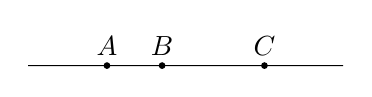
\begin{tikzpicture}
			\draw[fill=black] (0,0)--(1,0)node[above]{\(A\)}circle(1pt)
			--(1.7,0)node[above]{\(B\)}circle(1pt)
			--(3,0)node[above]{\(C\)}circle(1pt)
			--(4,0);
		\end{tikzpicture}
		\caption{直线上点的顺序}
		\label{figure:欧氏几何.直线上点的顺序1}
	\end{figure}

	\item 对于两点\(A\)和\(B\)(如\cref{figure:欧氏几何.直线上点的顺序2}),
	直线\(AB\)上恒至少有一点\(C\),使得\(B\)在\(A\)和\(C\)之间.
	\begin{figure}[ht]
		\centering
		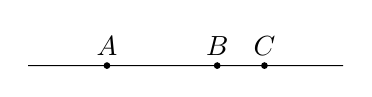
\begin{tikzpicture}
			\draw[fill=black] (0,0)--(1,0)node[above]{\(A\)}circle(1pt)
			--(2.4,0)node[above]{\(B\)}circle(1pt)
			--(3,0)node[above]{\(C\)}circle(1pt)
			--(4,0);
		\end{tikzpicture}
		\caption{直线上点的顺序}
		\label{figure:欧氏几何.直线上点的顺序2}
	\end{figure}

	\item 一直线的任意三点中,至多有一点在其他两点之间.
\end{enumerate}
\end{axiom}

在上述三条{\bf 直线顺序公理}之外,还需要一条{\bf 平面顺序公理}.

\begin{axiom}[顺序公理II]\label{axiom:欧氏几何.顺序公理2}
考虑一直线\(l\)上的两点\(A\)和\(B\).
我们把这一对点\(A\)和\(B\)确定的介于它们的点的集合叫做一条\DefineConcept{线段},记作\(AB\)(或\(BA\)).
在\(A\)和\(B\)之间的点叫做线段\(AB\)的点,或线段\(AB\)的\DefineConcept{内点};
\(A\)和\(B\)叫做线段\(AB\)的\DefineConcept{端点};
直线\(l\)上的其他点叫做线段\(AB\)的\DefineConcept{外点}.
\begin{enumerate}
	\setcounter{enumi}{3}
	\item 设\(A\)、\(B\)和\(C\)是不在同一直线上的三点,
	\(l\)是平面\(ABC\)上的一直线,
	但\(l\)不通过\(A,B,C\)这三点中的任一点
	(如\cref{figure:欧氏几何.平面上点的顺序1}),
	若直线\(l\)通过线段\(AB\)的一点,则它必定也通过线段\(AC\)或线段\(BC\)的一点.
	\begin{figure}[ht]
		\centering
		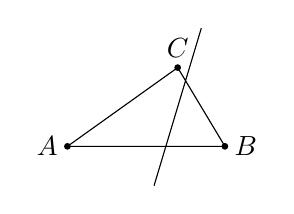
\begin{tikzpicture}
			\draw[fill=black] (-1,0)node[left]{\(A\)}circle(1pt)
			--(1,0)node[right]{\(B\)}circle(1pt)
			--(.4,1)node[above]{\(C\)}circle(1pt)--(-1,0)
			(.1,-.5)--(.7,1.5);
		\end{tikzpicture}
		\caption{平面上点的顺序}
		\label{figure:欧氏几何.平面上点的顺序1}
	\end{figure}
\end{enumerate}
\end{axiom}
直观地说,\cref{axiom:欧氏几何.顺序公理2} 说的就是:
若一直线“冲进”一个三角形的内部,它必定还要再“冲出”这个三角形.
易证:与线段\(AB\)相交的直线\(l\)不同时和\(AC,BC\)这两条线段都相交.

\subsection{关联公理和顺序公理的推论}
从\cref{axiom:欧氏几何.关联公理,axiom:欧氏几何.顺序公理1,axiom:欧氏几何.顺序公理2} 能推证下列定理.
\begin{theorem}\label{theorem:欧氏几何.定理3}
对于两点\(A\)和\(C\),直线\(AC\)上恒至少有一点\(D\),在\(A\)和\(C\)之间.
\begin{proof}
根据\cref{axiom:欧氏几何.关联公理} 第3条,直线\(AC\)外存在一点\(E\);
根据\cref{axiom:欧氏几何.顺序公理1} 第2条,直线\(AE\)上有一点\(F\),使得\(E\)在线段\(AF\)内.
根据\cref{axiom:欧氏几何.顺序公理1} 第2条、第3条,直线\(FC\)上有一点\(G\),不在线段\(FC\)内.
根据\cref{axiom:欧氏几何.顺序公理2} 第4条,直线\(EG\)必交线段\(AC\)于一点\(D\).
\end{proof}
\end{theorem}

\begin{theorem}\label{theorem:欧氏几何.定理4}
一直线上的任意三点\(A,B,C\)中,必有一点且只有一点在其他两点之间.
\begin{proof}
设\(A\)不在\(B\)和\(C\)之间,而且\(C\)不在\(A\)和\(B\)之间.
用直线连接\(B\)和直线\(AC\)外一点\(D\).
根据\cref{axiom:欧氏几何.顺序公理1} 第2条,能在直线\(BD\)上取一点\(G\),使得\(D\)在\(B\)和\(G\)之间.
对于三角形\(BCG\)和直线\(AD\)应用\cref{axiom:欧氏几何.顺序公理2} 第4条,可知直线\(AD\)通过线段\(CG\)内的一点\(E\);
同理可知直线\(CD\)通过线段\(AG\)内一点\(F\).
对于三角形\(AEG\)和直线\(CF\)应用\cref{axiom:欧氏几何.顺序公理2} 第4条,可知\(D\)在\(A\)和\(E\)之间;
再对于三角形\(AEC\)和直线\(BG\)应用\cref{axiom:欧氏几何.顺序公理2} 第4条,即证得\(B\)在\(A\)和\(C\)之间.
\end{proof}
\end{theorem}

\begin{theorem}\label{theorem:欧氏几何.定理5}
一直线上的任意四点\(A,B,C,D\),使得点\(B\)既在\(A\)和\(C\)之间,又在\(A\)和\(D\)之间;
而且点\(C\)既在\(A\)和\(D\)之间,又在\(B\)和\(D\)之间.
\end{theorem}

\begin{corollary}\label{theorem:欧氏几何.定理6}
一直线上的任意有限个点\(A,B,C,\dotsc,K\),
使得点\(B\)在\(A\)和\(C\),或和\(D\),或和\(E\),……,或和\(K\)之间;
而且点\(C\)在\(A\)(或\(B\))和\(D\),或和\(E\),……,或和\(K\)之间;以此类推.
\end{corollary}

\begin{corollary}\label{theorem:欧氏几何.定理7}
一直线上任意两点之间恒有无限多个点.
\end{corollary}

\begin{theorem}\label{theorem:欧氏几何.定理8}
一平面\(\gamma\)上的任一直线\(l\)将该平面上其余的点分为具有下述性质的两个区域:
一个区域的任一点\(A\)与另一区域的任一点\(B\)所决定的线段\(AB\)内,
必含有直线\(l\)的一点(如\cref{figure:欧氏几何.直线l分平面为两个区域});
而同一个区域的任意两点\(A\)和\(A'\)所决定的线段\(AA'\)内,不含有直线\(l\)的点.
\begin{figure}[ht]
\centering
\begin{tikzpicture}
\draw (-2,0)--(2,0)node[right]{\(l\)}
(.5,-1)node[right]{\(B\)}--(-.5,.5)node[left]{\(A\)}--(.3,1)node[right]{\(A'\)};
\end{tikzpicture}
\caption{直线\(l\)分平面为两个区域}
\label{figure:欧氏几何.直线l分平面为两个区域}
\end{figure}
\end{theorem}

\begin{definition}
我们说\(A\)和\(A'\)这两点在平面\(\gamma\)上直线\(l\)的\DefineConcept{同侧}%
(如\cref{figure:欧氏几何.直线l分平面为两个区域}),
而\(A\)和\(B\)这两点在平面\(\gamma\)上直线\(l\)的\DefineConcept{异侧}.
\end{definition}

\begin{definition}
设\(A,A',O\)和\(B\)是一直线\(l\)上的四点(如\cref{figure:欧氏几何.射线}),
而\(O\)在\(A\)和\(B\)之间,但不在\(A\)和\(A'\)之间.
我们称“\(A\)和\(A'\)这两点在\(l\)上点\(O\)的\DefineConcept{同侧}”,
而称“\(A\)和\(B\)这两点在\(l\)上点\(O\)的\DefineConcept{异侧}”.

直线\(l\)上点\(O\)的同侧的点的全体,叫做从点\(O\)起始的一条\DefineConcept{射线};
因此一直线的每一点把这直线分成两条射线.
\begin{figure}[ht]
\centering
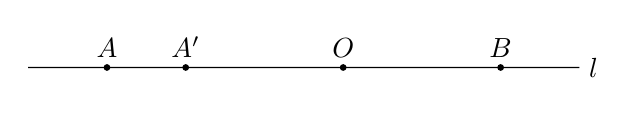
\begin{tikzpicture}
\draw[fill=black] (-3,0)--(-2,0)node[above]{\(A\)}circle(1pt)
--(-1,0)node[above]{\(A'\)}circle(1pt)
--(1,0)node[above]{\(O\)}circle(1pt)
--(3,0)node[above]{\(B\)}circle(1pt)--(4,0)node[right]{\(l\)};
\end{tikzpicture}
\caption{射线}
\label{figure:欧氏几何.射线}
\end{figure}
\end{definition}

\begin{definition}
若干条首尾相连的线段\(AB,BC,CD,\dotsc,KL\)的集合叫做一条\DefineConcept{折线段},
它连结\(A\)和\(L\)这两点.
为求简便,可将这条折线段记为\(ABCD \dotso KL\).
线段\(AB,BC,CD,\dotsc,KL\)的内点和端点都叫做这条折线段的点.
点\(A\)和点\(L\)称为“折线段的\DefineConcept{端点}”.

若折线段\(ABCD \dotso KL\)的顶点\(A,B,C,D,\dotsc,K,L\)都在同一平面上,
且它的端点\(L\)和\(A\)是同一个点,
则这条折线段就叫做一个\DefineConcept{多边形},
记为\(ABCD \dotso K\).
线段\(AB,BC,CD,\dotsc,KA\)叫做“多边形的\DefineConcept{边}”.
点\(A,B,C,D,\dotsc,K\)叫做“多边形的\DefineConcept{顶点}”.

若一个多边形有三个顶点,
则称之为\DefineConcept{三角形}.
设三角形的三个顶点分别为\(A\)、\(B\)、\(C\),
则可将其表记为以下六个符号中的任意一个:
\[
\begin{split}
\triangle ABC, \qquad
\triangle ACB, \qquad
\triangle BAC, \\
\triangle BCA, \qquad
\triangle CAB, \qquad
\triangle CBA.
\end{split}
\]

若一个多边形有\(n\ (n>3)\)个顶点,
则称之为\(n\) \DefineConcept{边形}.

若一个多边形的顶点各各不同,
它的任一边内不含有顶点,
且它的任意两边无公共点,
这个多边形就叫做\DefineConcept{简单多边形}.
\end{definition}

根据\cref{theorem:欧氏几何.定理8} 可以推出下列两条推论:
\begin{theorem}\label{theorem:欧氏几何.定理9}
一平面\(\alpha\)上的每一个简单多边形,
把平面\(\alpha\)上其余点%
(即平面\(\alpha\)上的,
而不在这多边形的边上的点)%
分为\DefineConcept{内域}和\DefineConcept{外域}两个区域.
这两个区域具有如下性质:
\begin{enumerate}
	\item 若\(A\)是“内域的一个点(内点)”,
	而且\(B\)是“外域的一个点(外点)”,
	则平面\(\alpha\)上任意一条连接\(A\)和\(B\)的折线段,
	至少和多边形有一公共点.

	\item 若\(A\)和\(C\)是内点,
	而\(B\)和\(D\)是外点,
	则在平面\(\alpha\)上恒有连接\(A\)和\(C\)的折线段,
	和连接\(B\)和\(D\)的折线段,
	它们都和多边形无公共点.

	\item 平面\(\alpha\)上存在全含于外域的直线,
	而不存在全含于内域的直线.
\end{enumerate}
\end{theorem}

\begin{theorem}\label{theorem:欧氏几何.定理10}
每一平面\(\alpha\)把空间中其余点分为具有下述性质的两个区域:
\begin{enumerate}
	\item 一区域的任一点\(A\)和另一区域的任一点\(B\)所决定的线段\(AB\)内,必含有\(\alpha\)的一点.
	\item 同一区域的任意两点\(A\)和\(C\)所决定的线段\(AC\)内,恒不含有\(\alpha\)的点.
\end{enumerate}
\end{theorem}

\begin{definition}
在\cref{theorem:欧氏几何.定理10} 的条件下,
我们说“\(A\)和\(C\)这两点在空间中平面\(\alpha\)的\DefineConcept{同侧}”,
说“\(A\)和\(B\)这两点在空间中平面\(\alpha\)的\DefineConcept{异侧}”.
\end{definition}

\subsection{第三组公理:合同公理}
本组公理规定“合同”这个概念,利用它就可以规定运动的概念.

我们首先介绍角的概念.
\begin{definition}\label{definition:欧氏几何.几何元素.角}
设\(\alpha\)是任意平面,
而且\(h\)和\(k\)是\(\alpha\)上的、%
从一点\(A\)起始的、%
不属于同一直线的%
两条射线,
我们把这一对射线\(h\)和\(k\)所成的射线组叫做一个\DefineConcept{角},
记作\(\angle(h,k)\)或\(\angle(k,h)\).
称射线\(h\)和\(k\)为这个角的\DefineConcept{边}.
称点\(A\)为这个角的\DefineConcept{顶点}.

如果在\(h\)上任取一点记为\(B\),在\(k\)上任取一点记为\(C\),
那么也称角\(\angle(h,k)\)为\(\angle BAC\)或\(\angle A\).
不致混淆时,也可以用小写希腊字母表记角.

记射线\(h\)所在的直线为\(p\),射线\(k\)所在的直线为\(q\).
射线\(h\)与\(k\)(包括点\(A\))把平面\(\alpha\)上其余点分成两个区域:
在\(q\)的\(h\)侧(即\(h\)的点所在的那一侧)的,且%
在\(p\)的\(k\)侧(即\(k\)的点所在的那一侧)的区域,
叫做“角\(\angle(h,k)\)的\DefineConcept{内部}”,
或者说是在\DefineConcept{角内};
其他区域叫做“角\(\angle(h,k)\)的\DefineConcept{外部}”,
或者说是在\DefineConcept{角外}.
\end{definition}

\begin{property}
根据第一组和第二组公理,
易知任意角(不妨设为交于点\(A\)的射线\(h\)、\(k\)所成的角,即\(\angle(h,k)\))具有以下性质:
\begin{enumerate}
\item 角内、角外两个区域各含有点,连结角内两点的线段完全在角内.
\item 若点\(H\)在射线\(h\)上,点\(K\)在射线\(k\)上,则线段\(HK\)完全在角内.
\item 一条从点\(A\)起始的射线,要么完全在角内,要么完全在角外.
\item 一条完全在角内的射线与线段\(HK\)有交点.
\item 若\(B\)是一个区域的一点,而且\(C\)是另一个区域的一点,
则每一条连接\(B\)和\(C\)的折线段,要么通过点\(A\),要么与\(h\)或\(k\)至少有一个交点;
反之,若\(B\)和\(D\)是同一个区域的两点,则恒有一条连接\(B\)和\(D\)的折线段,
它既不通过点\(A\),又与\(h\)、\(k\)无交点.
\end{enumerate}
\end{property}


\begin{axiom}[合同公理]\label{axiom:欧氏几何.合同公理}
线段与线段之间、角与角之间都有一定的相互关系,我们用“合同”或“相等”这个词来描述.
\begin{enumerate}
\item 设\(A\)和\(B\)是直线\(a\)上的两点,
\(P\)是直线\(b\)上的点,
而且给定了直线\(b\)上\(P\)的一侧,
则在直线\(b\)上\(P\)的这一侧,
恒有一点\(Q\),
使得线段\(AB\)和线段\(PQ\)合同.
我们将上述关系记为\(AB \equiv PQ\).

\item 若两线段\(PQ\)和\(MN\)都和线段\(AB\)合同,
则\(PQ\)和\(MN\)也合同.

\item 设两线段\(AB\)和\(BC\)在同一直线\(a\)上,无公共点,
而且两线段\(PQ\)和\(QR\)在同一直线\(b\)上,亦无公共点.
若\(AB \equiv PQ\)且\(BC \equiv QR\),
则\(AC \equiv PR\).

\item 设给定了一个平面\(\alpha\)上的一个角\(\angle(h,k)\),
一平面\(\beta\)上的一直线\(b\),
和在\(\beta\)上\(b\)的一侧.
设\(p\)是\(b\)上的、从点\(B\)起始的一条射线,
则平面\(\beta\)上恰有一条射线\(q\),
使得\(\angle(h,k)\)与\(\angle(p,q)\)合同,
而且使得\(\angle(p,q)\)的内部在\(b\)的这给定了的一侧.
我们将上述关系记为\(\angle(h,k) \equiv \angle(p,q)\).

\item 若两个三角形\(ABC\)和\(PQR\)有下列合同式
\[
AB \equiv PQ, \qquad
AC \equiv PR, \qquad
\angle BAC \equiv \angle QPR,
\]
则也恒有合同式\footnote{%
只需要交换记号,还可以同时得到另一个合同式
\(\angle ACB \equiv \angle PRQ\)
也同时成立.
}
\[
\angle ABC \equiv \angle PQR.
\]
\end{enumerate}
\end{axiom}

我们在前面用点\(A\)、\(B\)所成的点组规定一条线段,并用\(AB\)或\(BA\)表示;
我们在线段的定义里,并不考虑这两点的顺序;
因此下列四个合同式的意义相同:
\[
AB \equiv PQ, \qquad
AB \equiv QP, \qquad
BA \equiv PR, \qquad
BA \equiv QP.
\]

如同线段我们不考虑它的方向,在角的定义中我们也不考虑旋转方向.
因此下列四个合同式的意义也相同:
\[
\angle(h,k) \equiv \angle(p,q), \qquad
\angle(h,k) \equiv \angle(q,p), \qquad
\angle(k,h) \equiv \angle(p,q), \qquad
\angle(k,h) \equiv \angle(q,p).
\]

\cref{axiom:欧氏几何.合同公理} 第3条要求线段能够相加.

\cref{axiom:欧氏几何.合同公理} 第4条可以表述为:
每一个角都能用唯一确定的方式迁移到一个给定了的平面上,
使得它沿着一条给定了的射线,并且在这射线的给定了的一侧.
藉此,我们直接保证了角的迁移的可能性与唯一性.

\cref{axiom:欧氏几何.合同公理} 第1条、第2条、第3条只论及线段的合同,
因此可以叫做“第三组公理中的直线公理”.

\cref{axiom:欧氏几何.合同公理} 第4条论及角的合同.
\cref{axiom:欧氏几何.合同公理} 第5条则把线段的合同和角的合同这两个概念联系起来.
这两条概念论及平面几何的几何元素,
因此可以叫做“第三组公理中的平面公理”.

\cref{axiom:欧氏几何.合同公理} 第1条要求线段平移的可能性,
但它还没有保证这种平移的唯一性.
只有结合\cref{axiom:欧氏几何.合同公理} 第5条,
从角的迁移的唯一性出发予以证明.
具体地,我们应用反证法,
假设把线段\(PQ\)迁移到一条从\(A\)起始的射线上可以得到不同的两点\(B\)、\(D\);
在直线\(AB\)外取一点\(C\),于是有下列合同式
\[
AB \equiv AD, \qquad
AC \equiv AC, \qquad
\angle BAC \equiv \angle DAC;
\]
那么根据\cref{axiom:欧氏几何.合同公理} 第5条,得
\[
\angle ACB \equiv \angle ACD;
\]
这和\cref{axiom:欧氏几何.合同公理} 第4条中要求的角的迁移的唯一性矛盾,
因此线段平移也是唯一的.

\begin{property}
线段的合同关系具有自反性、对称性和传递性,即
\begin{enumerate}
\item {\rm\bf 自反性},
\(AB \equiv AB\).

\item {\rm\bf 对称性},
\(AB \equiv PQ \implies PQ \equiv AB\)
\footnote{%
正因线段的合同关系具有对称性,
我们才能说“某两条线段互相合同”.
}.

\item {\rm\bf 传递性},
\(AB \equiv PQ \land PQ \equiv MN \implies AB \equiv MN\).
\end{enumerate}
\end{property}

\begin{property}
角的合同关系具有自反性、对称性和传递性,即
\item {\rm\bf 自反性},
\(\angle(h,k) \equiv \angle(h,k)\).

\item {\rm\bf 对称性},
\(\angle(h,k) \equiv \angle(p,q)
\implies
\angle(p,q) \equiv \angle(h,k)\).

\item {\rm\bf 传递性},
\(\angle(h,k) \equiv \angle(m,n)
\land
\angle(m,n) \equiv \angle(p,q)
\implies
\angle(h,k) \equiv \angle(p,q)\).
\end{property}
角的合同关系的自反性是显然的,
至于它的对称性、传递性和可加性,
则留待以后予以证明.

\subsection{合同公理的推论}
\begin{definition}
两角共顶点,共一边,而且不公共的两边合成一条直线的,叫做\DefineConcept{邻补角}.
\end{definition}
\begin{definition}
两角共顶点,而且它们的边合成两条直线的,叫做\DefineConcept{对顶角}.
\end{definition}
\begin{definition}
一个角和它的邻补角合同的,叫做\DefineConcept{直角}.
\end{definition}

\begin{theorem}\label{theorem:欧氏几何.定理11}
若一个三角形中的两边合同,和这两边相对的两角就也合同\footnote{%
换言之,等腰三角形的底角相等.
}.
\end{theorem}

\begin{definition}
若两个三角形\(ABC\)和\(PQR\)满足下列所有的合同式
\[
\begin{split}
AB \equiv PQ, \qquad
AC \equiv PR, \qquad
BC \equiv QR, \\
\angle A \equiv \angle P, \qquad
\angle B \equiv \angle Q, \qquad
\angle C \equiv \angle R,
\end{split}
\]
就说“三角形\(ABC\)合同于三角形\(PQR\)”,
或者说“三角形\(ABC\)和三角形\(PQR\)是全等三角形”,
或者说“三角形\(ABC\)、\(PQR\)全等”,
记为\(\triangle ABC \cong \triangle PQR\).
\end{definition}

\begin{theorem}[三角形的合同定理1]\label{theorem:欧氏几何.定理12}
若两个三角形\(ABC\)、\(PQR\)有下列合同式
\[
AB \equiv PQ, \qquad
AC \equiv PR, \qquad
\angle A \equiv \angle P,
\]
则\(\triangle ABC \cong \triangle PQR\).
\end{theorem}

\begin{theorem}[三角形的合同定理2]\label{theorem:欧氏几何.定理13}
若两个三角形\(ABC\)、\(PQR\)有下列合同式
\[
AB \equiv PQ, \qquad
\angle A \equiv \angle P,
\angle B \equiv \angle Q,
\]
则\(\triangle ABC \cong \triangle PQR\).
\end{theorem}

\begin{theorem}\label{theorem:欧氏几何.定理14}
设\(\angle ABC\)的邻补角为\(\angle CBD\),
\(\angle PQR\)的邻补角为\(\angle RQS\).
若\(\angle ABC \equiv \angle PQR\),
则\(\angle CBD \equiv \angle RQS\).
\end{theorem}

\begin{corollary}\label{theorem:欧氏几何.对顶角合同}
任意一个角和它的对顶角合同.
\end{corollary}

\begin{corollary}\label{theorem:欧氏几何.直角存在}
直角存在.
\begin{proof}
把任意一个角迁移到沿着一条从点\(O\)起始的射线\(OA\),
而且迁移到这射线的两侧.
在新得到的这两个角的另外两条边上,
取线段\(OB \equiv OC\),
线段\(BC\)交射线\(OA\)于一点\(D\).

若点\(D\)就是点\(O\),
\(\angle BOA\)和\(\angle COA\)是合同的邻补角,所以是直角.

若点\(D\)在射线\(OA\)上,
或在与\(OA\)恰好反向的射线上,
总有\(\angle DOB \equiv \angle DOC\);
根据\cref{axiom:欧氏几何.合同公理} 第2条,
每一条线段都和它自己合同,即\(OD \equiv OD\);
再根据\cref{axiom:欧氏几何.合同公理} 第5条,
就有\(\angle ODB \equiv \angle ODC\).
\end{proof}
\end{corollary}

\begin{theorem}\label{theorem:欧氏几何.定理15}
设\(h\)、\(k\)和\(l\)是一平面\(\alpha\)上的、从一点\(M\)起始的三条射线,
而且\(p\)、\(q\)和\(r\)是一平面\(\beta\)上的、从一点\(N\)起始的三条射线;%
又设\(h\)和\(k\)分别在\(l\)的同侧(或异侧),
且\(p\)和\(q\)也分别在\(r\)的同侧(或异侧).
若
\[
\angle(h,l) \equiv \angle(p,r)
\quad\text{且}\quad
\angle(k,l) \equiv \angle(q,r),
\]
则
\[
\angle(h,k) \equiv \angle(p,q).
\]
\end{theorem}

\begin{theorem}\label{theorem:欧氏几何.定理16}
设平面\(\alpha\)上的\(\angle(h,k)\)合同于平面\(\beta\)上的\(\angle(p,q)\),
而且\(l\)是平面\(\alpha\)上的、从\(\angle(h,k)\)的顶点起始的、在\(\angle(h,k)\)角内的一条射线.
这时平面\(\beta\)上恒恰有一条从\(\angle(p,q)\)的顶点起始的、在\(\angle(p,q)\)角内的一条射线\(r\),
使得
\[
\angle(h,l) \equiv \angle(p,r), \qquad
\angle(k,l) \equiv \angle(q,r).
\]
\end{theorem}

\begin{theorem}\label{theorem:欧氏几何.定理17}
若两点\(C\)和\(D\)在直线\(AB\)的异侧,
而且\(AC \equiv AD\)、\(BC \equiv BD\),
则\(\angle ABC \equiv \angle ABD\).
\end{theorem}

\begin{theorem}[三角形的合同定理3]\label{theorem:欧氏几何.定理18}
若两个三角形\(ABC\)和\(PQR\)的每对对应边合同,即
\[
AB \equiv PQ, \qquad
AC \equiv PR, \qquad
BC \equiv QR,
\]
则\(\triangle ABC \cong \triangle PQR\).
\end{theorem}

\begin{theorem}\label{theorem:欧氏几何.定理19}
若两个角\(\angle(a,b)\)和\(\angle(c,d)\)都合同于第三个角\(\angle(e,f)\),
则\(\angle(a,b)\)也合同于\(\angle(c,d)\).
\end{theorem}
由此,我们证明了角的合同关系具有对称性、传递性.

现在我们就可以比较角的大小了.

\begin{theorem}\label{theorem:欧氏几何.定理20}
如\cref{figure:欧氏几何.图20},
给定任意两个角\(\angle(h,k)\)和\(\angle(p,r)\).
设迁移\(\angle(h,k)\)到沿着\(p\),而且在\(p\)的\(r\)侧时,所得到的射线是\(q\);
又迁移\(\angle(p,r)\)到沿着\(h\),而且在\(h\)的\(k\)侧时,所得到的射线是\(l\);
这时,若\(q\)在\(\angle(p,r)\)内,则\(l\)在\(\angle(h,k)\)外.
反之也成立.
\end{theorem}

\begin{figure}[ht]
	\centering
	\begin{tikzpicture}
		\pgfmathsetmacro{\r}{3}
		\begin{scope}
			\draw(0,0)--(\r,0)node[right]{\(h\)};
			\pgfmathsetmacro{\kx}{\r*cos(45)}
			\pgfmathsetmacro{\ky}{\r*sin(45)}
			\draw(0,0)--(\kx,\ky)node[right]{\(k\)};
			\pgfmathsetmacro{\lx}{\r*cos(60)}
			\pgfmathsetmacro{\ly}{\r*sin(60)}
			\draw(0,0)--(\lx,\ly)node[above]{\(l\)};
		\end{scope}
		\begin{scope}[xshift=6cm]
			\draw(0,0)--(\r,0)node[right]{\(p\)};
			\pgfmathsetmacro{\kx}{\r*cos(45)}
			\pgfmathsetmacro{\ky}{\r*sin(45)}
			\draw(0,0)--(\kx,\ky)node[right]{\(q\)};
			\pgfmathsetmacro{\lx}{\r*cos(60)}
			\pgfmathsetmacro{\ly}{\r*sin(60)}
			\draw(0,0)--(\lx,\ly)node[above]{\(r\)};
		\end{scope}
	\end{tikzpicture}
	\caption{}
	\label{figure:欧氏几何.图20}
\end{figure}

\begin{definition}
在\cref{theorem:欧氏几何.定理20} 中,
若\(q\)在\(\angle(p,r)\)内,则称“\(\angle(h,k)\)小于\(\angle(p,r)\)”,记为\(\angle(h,k) < \angle(p,r)\).
若\(q\)在\(\angle(p,r)\)外,则称“\(\angle(h,k)\)大于\(\angle(p,r)\)”,记为\(\angle(h,k) > \angle(p,r)\).
\end{definition}

因此,两个角\(\alpha,\beta\)恒恰适合以下三种情形之一:
\begin{itemize}
	\item \(\alpha<\beta\)和\(\beta>\alpha\).
	\item \(\alpha\equiv\beta\).
	\item \(\alpha>\beta\)和\(\beta<\alpha\).
\end{itemize}

角的大小的比较有传递性.
若有下列三种情形
\begin{itemize}
	\item \(\alpha>\beta,\beta>\gamma\),
	\item \(\alpha>\beta,\beta\equiv\gamma\),
	\item \(\alpha\equiv\beta,\beta>\gamma\),
\end{itemize}
之一,则\[
	\alpha>\gamma.
\]

\begin{theorem}\label{theorem:欧氏几何.定理21}
所有的直角都互相合同.
\end{theorem}

\begin{definition}
一个角大于它的邻补角的,也就是大于一直角的,叫做\DefineConcept{钝角};
小于它的邻补角的,也就是小于一直角的,叫做\DefineConcept{锐角}.
\end{definition}

\begin{definition}
\(\triangle ABC\)的\(\angle ABC\)、\(\angle BCA\)和\(\angle CAB\)
叫做这个三角形的\DefineConcept{内角},简称为这个三角形的\DefineConcept{角};
它们的邻补角叫做这个三角形的\DefineConcept{外角}.
\end{definition}

\begin{theorem}[外角定理]\label{theorem:欧氏几何.定理22}
在三角形中,一个外角大于其任一不相邻的内角.
\end{theorem}

下列定理是外角定理的重要推论.

\begin{theorem}\label{theorem:欧氏几何.定理23}
在三角形中,长边所对的角大于短边所对的角.
\end{theorem}

\begin{theorem}\label{theorem:欧氏几何.定理24}
若三角形有两角合同,则有两边合同.
\end{theorem}
这是\cref{theorem:欧氏几何.定理11} 的逆定理,
也是\cref{theorem:欧氏几何.定理23} 的直接推论.

从\cref{theorem:欧氏几何.定理22},
还能很简单地证得下述对三角形的合同定理二的补充.
\begin{theorem}\label{theorem:欧氏几何.定理25}
若\(\triangle ABC\)和\(\triangle DEF\)有下列合同式\[
	AB \equiv DE, \qquad
	\angle A \equiv \angle D, \qquad
	\angle C \equiv \angle F,
\]
则这两个三角形合同.
\end{theorem}

\begin{theorem}\label{theorem:欧氏几何.定理26}
每一线段都能二等分.
\end{theorem}

类似地,从\cref{theorem:欧氏几何.定理11} 和\cref{theorem:欧氏几何.定理26},能直接推证下列事实:
\begin{theorem}
每一角都能二等分.
\end{theorem}

合同的概念可以推广应用到任意的图形上去.

\begin{definition}
设\(A,B,C,D,\dotsc,K,L\)是直线\(\alpha\)上的一个点列,
\(A',B',C',D',\dotsc,K',L'\)是直线\(\alpha'\)上的一个点列,
而且所有的对应线段都两两合同,
那么称这两个点列互相合同.
\(A\)和\(A'\)、\(B\)和\(B'\),一直到\(L\)和\(L'\),叫做这\emph{合同点列}的对应点.
\end{definition}

\begin{theorem}\label{theorem:欧氏几何.定理27}
两个合同的点列的点的顺序相同.
\end{theorem}

\begin{definition}
任意有限个点叫做一个\DefineConcept{图形}.
一个图形的点,若都在一个平面上,这图形就叫做一个\DefineConcept{平面图形}.
\end{definition}

两个图形的点之间若有一个一一对应的关系,
使得由此规定的每对对应的线段都互相合同,
且每对对应的角都互相合同,
那么这两个图形合同.

由\cref{theorem:欧氏几何.定理14}
和\cref{theorem:欧氏几何.定理27},
可知合同图形有下述性质:
若一个图形中的三个点在一条直线上,
则每一个和它合同图形中的对应的三个点也在一条直线上.
合同图形中的、对应平面上的对应点,
对于对应直线而言的顺序相同;
对应直线上的对应点顺序也相同.

平面的和空间的最普遍的合同定理如下:
\begin{theorem}\label{theorem:欧氏几何.定理28}
设\((A,B,C,\dotsc,L)\)
和\((A',B',C',\dotsc,L')\)
是两个合同的平面图形.
若\(P\)是第一个图形的平面上的一点,
则第二个图形的平面上恒有一点\(P'\)存在,
使得\((A,B,C,\dotsc,L,P)\)
和\((A',B',C',\dotsc,L',P')\)还是合同的图形.
若\((A,B,C,\dotsc,L)\)至少含有不在同一条直线上的三点,
则\(P'\)只有一个可能的作法.
\end{theorem}

\begin{theorem}\label{theorem:欧氏几何.定理29}
设\((A,B,C,\dotsc,L)\)
和\((A',B',C',\dotsc,L')\)
是两个合同的图形.
若\(P\)是任意一点,
则恒有一点\(P'\)存在,
使得\((A,B,C,\dotsc,L,P)\)
和\((A',B',C',\dotsc,L',P')\)还是合同的图形.
若\((A,B,C,\dotsc,L)\)至少含有不在同一平面上的四点,
则\(P'\)只有一个可能的作法.
\end{theorem}

\cref{theorem:欧氏几何.定理29} 说出了所有关于合同的空间事实,
因此,空间中运动的性质,都是上述的直线的和平面的五条合同公理(结合着第一组和第二组公理)的推论.

\subsection{第四组公理:平行公理}
设\(\alpha\)是任一平面,
\(a\)是\(\alpha\)上的任一直线,
而且\(A\)是\(\alpha\)上的、但不在\(a\)上的一点,
在\(\alpha\)上作一直线\(c\),
通过\(A\)且和\(a\)相交,
再在\(\alpha\)上作一直线\(b\),通过\(A\),
且使得\(c\)交\(a\)和\(b\)于相等的同位角.
从\hyperref[theorem:欧氏几何.定理22]{外角定理},
易知\(a\)和\(b\)这两直线无公共点,这就是说,
在一平面\(\alpha\)上,而且通过一直线\(a\)外的一点\(A\),
恒有一直线不和\(a\)相交.

现在可将平行公理叙述如下:
\begin{axiom}[平行公理、欧几里得公理]\label{axiom:欧氏几何.平行公理}
设\(a\)是任一直线,\(A\)是\(a\)外的任一点.
在\(a\)和\(A\)所决定的平面上,
至多有一条直线通过\(A\),而且不和\(a\)相交.
\end{axiom}

根据上文和平行公理,我们知道:
在\(a\)和\(A\)所决定的平面上,恰有一直线,通过\(A\)且不和\(a\)相交,
我们把这条直线叫做“通过\(A\)的\(a\)的\DefineConcept{平行直线}”.

平行公理和下述的要求等价:
如果一平面上的\(a\)和\(b\)两直线都不和这平面上的第三条直线\(c\)相交,
那么\(a\)和\(b\)也不相交.

事实上,如果\(a\)和\(b\)有一公共点\(A\),那么在同一平面上,
就有了\(a\)和\(b\)这两条直线,都通过\(A\)而且不和\(c\)相交.
这和平行公理矛盾.
反之,从上述要求,也易推得平行公理.

平行公理是一条平面公理.
它的引入,使得几何的基础大大地简单化了,也使得几何的构造容易得多了.

例如,在合同公理之外,再加上平行公理,不难得到下列熟知的事实:
\begin{theorem}\label{theorem:欧氏几何.定理30}
若两平行直线被第三条直线所截,则同位角合同,内错角也合同;
反之,若同位角合同,或内错角合同,则前两直线平行.
\end{theorem}

\begin{theorem}\label{theorem:欧氏几何.定理31}
三角形的三个内角的和等于两个直角的和.
\end{theorem}
\begin{figure}[ht]
	\centering
	\begin{tikzpicture}
		\coordinate (A) at (0,0);
		\coordinate (B) at (4,0);
		\coordinate (C) at (3,2);
		\coordinate (P) at (2,2);
		\coordinate (Q) at (4,2);
		\draw (A)node[left]{\(A\)}
				-- (B)node[right]{\(B\)}
				-- (C)node[above]{\(C\)} -- (A);
		\draw (P)node[left]{\(P\)} -- (Q)node[right]{\(Q\)};
		\draw pic[draw=blue,angle radius=5mm]{angle=B--A--C}
				pic[draw=blue,angle radius=6mm]{angle=B--A--C}
				pic[draw=blue,angle radius=5mm]{angle=P--C--A}
				pic[draw=blue,angle radius=6mm]{angle=P--C--A}
				pic[draw=orange,angle radius=4mm]{angle=C--B--A}
				pic[draw=orange,angle radius=4mm]{angle=B--C--Q};
	\end{tikzpicture}
	\caption{}
	\label{figure:欧氏几何.三角形内角和等于平角}
\end{figure}

\begin{definition}
设\(M\)是一平面\(\alpha\)上的任一点.
考虑\(\alpha\)上的所有的那些点\(A\),
它们使线段\(MA\)都互相合同的.
这种点\(A\)的全体叫做一个\DefineConcept{圆},
点\(M\)叫做“这个圆的\DefineConcept{中心}”,简称\DefineConcept{圆心}.
\end{definition}

根据这个定义,我们容易从第三组和第四组公理,推证关于圆的若干熟知的定理.
特别是下述的定理:
通过不在同一条直线上的三点,能作一圆;
关于同一条弦上的圆周角合同的定理;
关于内接于圆的一个四边形的角的定理.

\subsection{第五组公理:连续公理}

\begin{axiom}[连续公理]
关于线段、角的度量,有如下公理:
\begin{enumerate}
	\item (度量公理,阿基米德公理).
	若\(AB\)和\(CD\)是任意两线段,则必存在一个数\(n\)使得沿\(A\)到\(B\)的射线上,
	自\(A\)作首尾相接的\(n\)个线段\(CD\),必将越过\(B\)点.
	\item (直线完备公理).
	一直线上的点集联通其顺序关系与合同关系不可能再这样扩充,
	使得这直线上原来元素之间所具有的关系,
	从第一组、第二组、第三组公理所推出的直线顺序与合同的基本性质\footnote{%
	所谓“基本性质”是指第二组第一至三条公理和\cref{theorem:欧氏几何.定理5} 中所叙述的顺序性质,
	以及第三组第一至第三条公理中所叙述的合同性质连同迁移线段的唯一性.}
	以及度量公理都仍旧保持\footnote{%
	所谓“仍旧保持”是指,当点集扩充后,顺序关系及合同关系也将延续到扩充后的点集中去.
	我们注意到第一组第三条公理在各种扩充后,不言而喻地仍然保持,
	至于在所考虑的扩充下,\cref{theorem:欧氏几何.定理3} 仍能成立,
	则是保持阿基米德公理的结果.}.
\end{enumerate}
\end{axiom}

完备公理中所要求保持的诸公理之一是阿基米德公理,
这时完备公理从本质上能以建立所不可缺少的一个条件.
其实我们能够证明:
若直线上的一个点集能满足上面所列举的关于顺序公理和定理以及合同公理和定理,
这点集就恒能够增加新点,使扩充后的点集还满足这里所提到的诸公理;
也就是说,如果一条完备公理,只要求保持这里所提到的诸公理和定理,
但不要求保持阿基米德公理或一条等价的公理,就要产生矛盾.

这两条连续公理都是直线公理.

下面所述更普遍的定理,主要根据直线完备公理.
\begin{theorem}[完备定理]\label{theorem:欧氏几何.定理32}
几何元素(即点、直线、平面)形成一个集合,
它在保持关联公理、顺序公理、合同公理和阿基米德公理,
从而更不用说,在保持全体公理的条件之下,
不可能经由点、直线和平面再行扩充.
\end{theorem}

完备定理还能表成较强的形式.
也就是在完备定理内缩要求保持的诸公理中,有些并不是绝对需要的,为了定理能够成立,
重要的倒是在所要求保持的诸公理中包含有第一组第七条公理.
其实我们能证明:
对于满足第一至第第五组公理的元素集合,恒能给添加新的点、直线和平面,
使得扩充后的心机和能满足除去第一组第七条公理之外的全体公理;
这就是说,一条完备定理若不包含第一组第七条公理或一条等价的公理,就将引出矛盾.

完备公理不是阿基米德公理的一个推论.
实际上,只有阿基米德公理,连同第一至第四组公理,
并不足以证明我们的几何和通常的笛卡尔解析几何完全相同.
但是加上了完备公理(虽然这条公理并没有直接提到收敛的概念),
就能证明(相当于戴德金分割的)确界的存在,
和关于聚点存在的波尔查诺定理,
从而才证明欧氏几何和笛卡尔几何相同.

从上文可见,连续的要求,在本质上,分成两个不同的部分:
阿基米德公理和完备公理;
前者的作用是替连续的要求做准备,
后者为完成整个公理系统作基础.

在本章后面的研究中,我们主要只用阿基米德公理作根据,而普遍地不假设完备公理.

\section{平面三角形}

\begin{theorem}
三角形内角和为\(\pi\).
\begin{proof}
设有\(\triangle ABC\).
过点\(C\)作平行于线段\(AB\)的直线\(PQ\).

由内错角相等,有\[
\angle{PCA} = \angle{CAB}, \quad \angle{QCB} = \angle{CBA},
\]又由\(\angle{PCA}+\angle{ACB}+\angle{QCB}=\pi\),可得\[
\angle{CAB}+\angle{ACB}+\angle{QCB}=\pi.
\qedhere
\]
\end{proof}
\end{theorem}

\begin{theorem}[正弦定理]
设任意三角形\(\triangle ABC\)的外接圆半径为\(R\),则\begin{equation}
\frac{a}{\sin A}
= \frac{b}{\sin B}
= \frac{c}{\sin C}
= 2R.
\end{equation}
\end{theorem}

\begin{theorem}[余弦定理]
设任意三角形\(\triangle ABC\),有\begin{equation}
c^2 = a^2 + b^2 - 2ab \cos C.
\end{equation}
\end{theorem}
可以看出,勾股定理是余弦定理的特殊情况,即当\(C = \frac{\pi}{2}\)时,有\(\cos C=0\),于是\(c^2 = a^2 + b^2\).

\begin{theorem}[摩尔外德公式]
%@see: https://arxiv.org/pdf/1808.08049.pdf
设任意三角形\(\triangle ABC\),则\begin{gather}
	\frac{a+b}{c}
	= \frac{\cos[(A-B)/2]}{\sin(C/2)}, \\
	\frac{a-b}{c}
	= \frac{\sin[(A-B)/2]}{\cos(C/2)}.
\end{gather}
\end{theorem}

\begin{theorem}[正切定理]
设任意三角形\(\triangle ABC\),有\begin{equation}
\frac{a-b}{a+b} = \frac{\tan[(A-B)/2]}{\tan[(A+B)/2]}.
\end{equation}
\end{theorem}

\section{圆}
\subsection{圆的概念}
\subsection{圆的性质}
\subsection{圆的周长\ 圆周率}
\begin{definition}
定义:圆的周长\(C\)与其直径\(2R\)之比称为\DefineConcept{圆周率},记作\(\pi\),即\[
\pi = \frac{C}{2R}.
\]
\end{definition}
由于圆周率是一个常数,那么已知圆的直径(或半径)可以求得圆的周长,而已知圆的周长可以求得圆的直径(或半径).

\begin{property}
给定圆上任意一段弧,若它的角度为\(\theta\),那么弧长为\(\theta r\).
\end{property}

\begin{corollary}
如下图,在单位圆上,当圆弧的角度\(\theta\)为锐角,即\(0<\theta<\pi/2\)时,\(\theta > x\). \begin{center}
\begin{tikzpicture}[scale=4]
%\draw[help lines, color=gray!30, dashed] (0,0) grid (1,1);
\pgfmathsetmacro{\u}{sqrt(3)/2}
\coordinate (O) at (0,0);
\coordinate (A) at (\u,0);
\coordinate (B) at (\u,1/2);
\draw (1,0)arc[start angle=0,end angle=30,radius=1]node[midway,right]{\(\theta\)} -- (0,0)node[midway,above left]{\(1\)} -- (1,0)
	(A) -- (B)node[midway,left]{\(x\)};
\draw pic["\(\theta\)",draw=orange,-,angle eccentricity=1.7,angle radius=5mm]{angle=A--O--B} pic[draw=gray,-,angle radius=0.3cm]{right angle=B--A--O};
\end{tikzpicture}
\end{center}
\end{corollary}

\section{平面凸多边形}
\begin{theorem}
设凸多边形的边数为\(n\),则其内角和为\((n-2)\pi\).
\end{theorem}
如图,在凸多边形内部任取一点\(P\),连接该点与凸多边形各顶点,可以得到\(n\)个三角形.
因为三角形内角和为\(\pi\),所以\(n\)个三角形内角和的总和为\(n\pi\),
再减去各三角形\(\angle P\)之和\(2\pi\),可知凸\(n\)边形的内角和为\((n-2)\pi\).
\begin{figure}[htb]
	\centering
	\begin{tikzpicture}
		\coordinate (A1) at (0,2);
		\coordinate (A2) at (1.5,4);
		\coordinate (A3) at (3.6,3.5);
		\coordinate (A4) at (4,2.5);
		\coordinate (A5) at (3.5,1.2);
		\coordinate (A6) at (1,0.5);
		\coordinate (P) at (1.6,2.4);
		\draw[dashed,color=black!30] (P)--(A1) (P)--(A2)
			(P)--(A3) (P)--(A4) (P)--(A5) (P)--(A6);
		\draw (A1)node[left]{\(A\)}--(A2)node[above]{\(B\)}
			--(A3)node[above right]{\(C\)}
			--(A4)node[right]{\(D\)}
			--(A5)node[below right]{\(E\)}
			--(A6)node[below]{\(F\)}--(A1)
			(P)node[right]{\(P\)};
		\fill (P)circle(2pt);
	\end{tikzpicture}
	\caption{}
\end{figure}

\begin{theorem}
凸多边形的外角和为\(2\pi\).
\end{theorem}

\section{凸多面体}
\begin{theorem}[欧拉公式]
设凸多面体的顶点数、棱数、面数分别为\(V\)、\(E\)、\(F\),则有\[
	V - E + F = 2.
\]
\end{theorem}

\begin{definition}
\DefineConcept{正凸多面体}(简称\DefineConcept{正多面体}),
是指满足以下条件的凸多面体:
\begin{enumerate}
	\item 正多面体的面由正多边形构成;
	\item 正多面体的各个顶角相等;
	\item 正多面体的各条棱长相等.
\end{enumerate}
\end{definition}

\begin{corollary}
正凸多面体只有5种:三四面体、正方体、正八面体、正十二面体、正二十面体.
\end{corollary}


\chapter{解析几何}
古希腊的毕达哥拉斯曾经提出“万物皆数”这一哲学观点,从这一章开始,我们研究如何利用代数方法研究几何问题.

在利用函数图像研究初等函数的性质时,我们产生了这么一个观念:
在平面上建立了平面直角坐标系以后,
平面上的点与数是一一对应的,
或说平面上的点与由实有序对\((x,y)\)一一对应.
几何图形是由点构成的集合,我们自然地想到能不能用数的集合来代表几何图形.
这就是解析几何的思想根源.



\section{向量及其线性运算}
解析几何最基本的方法是坐标法,即建立一个坐标系,使得点可以用有序对或元组来表示,
从而可以用方程表示图形,通过方程来研究图形的性质.
坐标法的优越性在于它利用了数可以进行运算的优点.
那么,能否把代数运算直接引入几何中来呢?什么样的几何对象能够做运算?

\subsection{向量的概念}
既有大小、又有方向的量,称为\DefineConcept{向量}或\DefineConcept{矢量}(vector).

与向量相对的,只有大小,没有方向的量,称为\DefineConcept{标量}(scalar).

我们通常用黑体小写拉丁字母(如\(\vb{a}\)、\(\vb{r}\)、\(\vb{v}\)、\(\vb{F}\)等),
或在小写拉丁字母上面加箭头(如\(\vec{a}\)、\(\vec{r}\)、\(\vec{v}\)、\(\vec{F}\)等)来表记向量.

在几何空间中,我们常用\DefineConcept{有向线段}(directed line segment)表示向量.
如\cref{figure:解析几何.有向线段} 所示,
对于一个给定的向量\(\vb{a}\),
我们可以用有向线段\(\vec{AB}\)来表示它,
其中用这条线段的长度\(\abs{AB}\)表示\(\vb{a}\)的大小,
用点\(A\)到点\(B\)的指向表示\(\vb{a}\)的方向.
我们把点\(A\)称为“有向线段\(\vec{AB}\)的\DefineConcept{起点}(initial point)”,
把点\(B\)称为“有向线段\(\vec{AB}\)的\DefineConcept{终点}(terminal point)”.
\begin{figure}[ht]
\centering
\begin{tikzpicture}[>=Stealth]
	\draw[->] (0,0)node[left]{\(A\)}--(3,1)node[right]{\(B\)}
		node[midway,above]{\(\vb{a}\)};
\end{tikzpicture}
\caption{有向线段}
\label{figure:解析几何.有向线段}
\end{figure}

规定长度相等、方向相同的有向线段表示同一个向量.

如\cref{figure:解析几何.有向线段的平移不变性} 所示,
若有向线段\(\vec{AB}\)表示向量\(\vb{a}\),
则\(\vec{AB}\)经过平行移动得到的有向线段\(\vec{CD}\)仍然表示向量\(\vb{a}\),
即\(\vb{a} = \vec{AB} = \vec{CD}\).
换言之,给定两条有向线段,如果其中一条经过平移可以让这两条有向线段的起点和终点分别完全重合,
那么这两条有向线段表示的是同一个向量.
\begin{figure}[ht]
\centering
\begin{tikzpicture}[>=Stealth]
	\draw[dashed] (0,0)--(5,0) (3,1)--(8,1);
	\draw[->] (0,0)node[left]{\(A\)}--(3,1)node[above left]{\(B\)}node[midway,above left]{\(\vb{a}\)};
	\draw[->] (5,0)node[below right]{\(C\)}--(8,1)node[right]{\(D\)};
\end{tikzpicture}
\caption{}
\label{figure:解析几何.有向线段的平移不变性}
\end{figure}

我们今后把向量的大小称为
“向量的\DefineConcept{长度}(length)”或“向量的\DefineConcept{模}(modulus)”,
记作\(\abs{\vb{a}}\).

如果两个向量\(\vb{a}\)和\(\vb{b}\)的长度相等、方向相同,
我们就说“\(\vb{a}\)和\(\vb{b}\)是\DefineConcept{相等}的”,
或者说“\(\vb{a}\)等于\(\vb{b}\)”,
记作\(\vb{a}=\vb{b}\);
否则,记\(\vb{a}\neq\vb{b}\).

长度为零的向量称为\DefineConcept{零向量}(zero vector),记作\(\vb{0}\).

看作有向线段时,零向量的起点和终点重合,所以它的方向可以看作是任意的、不确定的.

相对地,长度不为零的向量称为\DefineConcept{非零向量}(nonzero vector).

长度为1的向量称为\DefineConcept{单位向量}(identity vector),记作\(\vb{e}\).

任意给定一个向量\(\vb{a}\),与\(\vb{a}\)同向的单位向量记作\(\vb{a}^0\),
称其为“\(\vb{a}\)的\DefineConcept{方向}(direction)”.

任意给定一个向量\(\vb{a}\),
如果向量\(\vb{b}\)正好是与\(\vb{a}\)长度相等、方向相反的向量,
那么称“\(\vb{b}\)是\(\vb{a}\)的\DefineConcept{负向量}(negative vector)”,
记作\(-\vb{a}\).
例如,\(\vec{BA}\)是\(\vec{AB}\)的负向量,因此\(\vec{BA} = -\vec{AB}\).

\subsection{向量的加法}
我们知道,将与点\(A\)重合的点\(P\)移动到点\(B\)再移动到点\(C\)的结果是点\(P\)与点\(C\)重合.

\begin{definition}
%@see: 《解析几何》(丘维声) P2 定义1.1
对于向量\(\vb{a},\vb{b}\),
如\cref{figure:解析几何.向量相加的三角形法则} 所示,
作有向线段\(\vec{AB}\)表示\(\vb{a}\),
作有向线段\(\vec{BC}\)表示\(\vb{b}\),
把有向线段\(\vec{AC}\)表示的向量\(\vb{c}\)称为
“向量\(\vb{a}\)与\(\vb{b}\)的\DefineConcept{和}”,
记作\[
	\vec{AB}+\vec{BC}=\vec{AC}
	\quad\text{或}\quad
	\vb{c}=\vb{a}+\vb{b}.
\]
\end{definition}
由上述公式表示的向量加法规则通常称为\DefineConcept{三角形法则}(triangle law).
除此以外,我们还有\DefineConcept{平行四边形法则}(parallelogram law),
如\cref{figure:解析几何.向量相加的平行四边形法则}.

\begin{figure}[ht]
	\centering
	\def\subwidth{.4\linewidth}
	\begin{subfigure}[b]{\subwidth}
		\centering
		\begin{tikzpicture}
			\pgfmathsetmacro{\xmax}{5}
			\pgfmathsetmacro{\xmin}{0}
			\pgfmathsetmacro{\ymax}{4}
			\pgfmathsetmacro{\ymin}{0}
			\draw[help lines,color=gray!30,dashed](\xmin,\ymin)grid(\xmax,\ymax);
			\begin{scope}[->,>=Stealth,ultra thick]
				\draw(\xmin,0)--(\xmax,0)node[right]{\(x\)};
				\draw(0,\ymin)--(0,\ymax)node[above]{\(y\)};
			\end{scope}
			\coordinate(A)at(1,1);
			\coordinate(B)at(4,2);
			\coordinate(C)at(3,3);
			\begin{scope}[>=Stealth,->]
				\draw[blue](A)node[black,left]{\(A\)}
					--(B)node[black,right]{\(B\)}node[black,midway,below]{\(\vb{a}\)};
				\draw[blue](B)
					--(C)node[black,above]{\(C\)}node[black,midway,above right]{\(\vb{b}\)};
				\draw[red](A)--(C)node[black,midway,above left]{\(\vb{a}+\vb{b}\)};
			\end{scope}
		\end{tikzpicture}
		\caption{向量加法的三角形法则}
		\label{figure:解析几何.向量相加的三角形法则}
	\end{subfigure}
	\begin{subfigure}[b]{\subwidth}
		\centering
		\begin{tikzpicture}
			\pgfmathsetmacro{\xmax}{6}
			\pgfmathsetmacro{\xmin}{0}
			\pgfmathsetmacro{\ymax}{4}
			\pgfmathsetmacro{\ymin}{0}
			\draw[help lines,color=gray!30,dashed](\xmin,\ymin)grid(\xmax,\ymax);
			\begin{scope}[->,>=Stealth,ultra thick]
				\draw(\xmin,0)--(\xmax,0)node[right]{\(x\)};
				\draw(0,\ymin)--(0,\ymax)node[above]{\(y\)};
			\end{scope}
			\coordinate(A)at(2,1);
			\coordinate(B)at(5,2);
			\coordinate(C)at(4,3);
			\coordinate(D)at(1,2);
			\begin{scope}[>=Stealth,->]
				\draw[blue](A)node[black,below]{\(A\)}
					--(B)node[black,midway,below]{\(\vb{a}\)};
				\draw[blue](A)--(D)node[black,midway,left]{\(\vb{b}\)};
				\draw[red](A)--(C)node[black,midway,above left]{\(\vb{a}+\vb{b}\)};
			\end{scope}
			\draw[dashed](D)node[black,left]{\(D\)}
				--(C)node[black,above]{\(C\)}
				--(B)node[black,right]{\(B\)};
		\end{tikzpicture}
		\caption{向量相加的平行四边形法则}
		\label{figure:解析几何.向量相加的平行四边形法则}
	\end{subfigure}
	\caption{}
\end{figure}

向量的加法服从以下运算律:
\begin{enumerate}
	\item 结合律,即对于\(\forall \vb{a},\vb{b},\vb{c}\),有\[
		(\vb{a}+\vb{b})+\vb{c}
		= \vb{a}+(\vb{b}+\vb{c}).
	\]

	\item 交换律,即对于\(\forall \vb{a},\vb{b}\),有\[
		\vb{a}+\vb{b} = \vb{b}+\vb{a}.
	\]

	\item 对于\(\forall \vb{a}\),有\[
		\vb{a}+\vb{0}=\vb{a}.
	\]

	\item 对于\(\forall \vb{a}\),有\[
		\vb{a}+(-\vb{a})=\vb{0}.
	\]
\end{enumerate}
这些运算律都可以利用有向线段作图予以证明.

\begin{definition}
%@see: 《解析几何》(丘维声) P4 定义1.2
对于向量\(\vb{a},\vb{b}\),
称\(\vb{a}\)与\(\vb{b}\)的负向量\(-\vb{b}\)的和\(\vb{a}+(-\vb{b})\)为
“向量\(\vb{a}\)与\(\vb{b}\)的\DefineConcept{差}”,记作\(\vb{a}-\vb{b}\),即\[
	\vb{a}-\vb{b}
	\defeq
	\vb{a}+(-\vb{b}).
\]
\end{definition}

\begin{theorem}
%@see: 《解析几何》(丘维声) P10 习题1.1 7.
对任意向量\(\vb{a},\vb{b}\),都有\[
	\abs{\vb{a}+\vb{b}} \leq \vb{a} + \vb{b}.
\]
\end{theorem}

\subsection{向量的数量乘法}
\begin{definition}
%@see: 《解析几何》(丘维声) P4 定义1.3
规定:实数\(\lambda\)与向量\(\vb{a}\)的乘积\(\lambda \vb{a}\)还是一个向量,
它的长度为\[
\abs{\lambda\vb{a}}
\defeq
\abs{\lambda} \abs{\vb{a}},
\]
它的方向当\(\lambda>0\)时与\(\vb{a}\)相同,
当\(\lambda<0\)时与\(\vb{a}\)相反.
\end{definition}

对于任意向量\(\vb{a}\),
由于\(\abs{0 \vb{a}} = 0 \abs{\vb{a}} = 0\),
所以\(0 \vb{a} = \vb{0}\).
同理,对一切实数\(\lambda\),都有\(\lambda \vb{0} = \vb{0}\).

对于任意非零向量\(\vb{a}\),
因为向量\(\abs{\vb{a}}^{-1} \vb{a}\)与\(\vb{a}\)同向,
且\[
	\abs{\frac{1}{\abs{\vb{a}}} \vb{a}}
	= \frac{1}{\abs{\vb{a}}} \abs{\vb{a}} = 1,
\]
所以\(\vb{a}^0 = \abs{\vb{a}}^{-1} \vb{a}\).
像这样,把一个非零向量\(\vb{a}\)乘以它的长度的倒数,
以得到与它同向的单位向量\(\vb{a}^0\)的过程,称为“把\(\vb{a}\) \DefineConcept{单位化}”.

向量的数量乘法服从以下运算律:
对于任意向量\(\vb{a},\vb{b}\)和任意实数\(\lambda,\mu\),有
\begin{enumerate}
	\item \(1 \vb{a} = \vb{a}\);
	\item \((-1) \vb{a} = -\vb{a}\);
	\item \(\lambda(\mu \vb{a}) = (\lambda \mu) \vb{a}\);
	\item \((\lambda+\mu) \vb{a} = \lambda \vb{a} + \mu \vb{a}\);
	\item \(\lambda (\vb{a}+\vb{b}) = \lambda \vb{a} + \lambda \vb{b}\).
\end{enumerate}

\subsection{共线、共面的向量组}
向量的加法和数量乘法统称为向量的\DefineConcept{线性运算}.

设\(\AutoTuple{\vb{a}}{n}\)是一组向量,
\(\AutoTuple{k}{n}\)是一组实数,
则\(k_1 \vb{a}_1 + k_2 \vb{a}_2 + \dotsb + k_n \vb{a}_n\)是一个向量,
我们称其为“向量组\(\AutoTuple{\vb{a}}{n}\)的一个\DefineConcept{线性组合}”,
称\(\AutoTuple{k}{n}\)为这个线性组合的\DefineConcept{系数}.

\begin{definition}
%@see: 《解析几何》(丘维声) P6 定义1.4
若用起点相同的有向线段表示向量组中的向量,
这些向量的终点和它们的公共起点都在同一条直线上,
则称这个向量组是\DefineConcept{共线的}.

若用起点相同的有向线段表示向量组中的向量,
这些向量的终点和它们的公共起点都在同一个平面上,
则称这个向量组是\DefineConcept{共面的}(coplanar).
\end{definition}

\begin{theorem}
%@see: 《解析几何》(丘维声) P6 命题1.1
若\(\vb{a}\)与\(\vb{b}\)共线,且\(\vb{a}\neq\vb{0}\),
则存在唯一的实数\(\lambda\),使得\(\vb{b} = \lambda \vb{a}\).
\end{theorem}

\begin{theorem}\label{theorem:解析几何.两向量共线的充分必要条件1}
%@see: 《解析几何》(丘维声) P6 命题1.2
\(\vb{a}\)与\(\vb{b}\)共线的充分必要条件是:
存在不全为零的实数\(\lambda\)和\(\mu\),使得\[
	\lambda \vb{a} + \mu \vb{b} = \vb{0}.
\]
\begin{proof}
先证必要性.
设\(\vb{a}\)与\(\vb{b}\)共线.
若\(\vb{a}=\vb{b}=\vb{0}\),
则有\(1\vb{a}+1\vb{b}=\vb{0}\).
若\(\vb{a},\vb{b}\)不全为\(\vb{0}\),不妨设\(\vb{a}\neq\vb{0}\),
则存在实数\(\lambda\),使得\(\vb{b}=\lambda\vb{a}\),从而有\[
	\lambda\vb{a}+(-1)\vb{b}=\vb{0}.
\]

再证充分性.
若有不全为零的实数\(\lambda,\mu\),使得\(\lambda \vb{a} + \mu \vb{b} = \vb{0}\)成立,
不妨设\(\lambda\neq0\),于是得\(\vb{a}=-\frac{\mu}{\lambda}\vb{b}\),
因此\(\vb{a}\)与\(\vb{b}\)共线.
\end{proof}
\end{theorem}

\begin{corollary}\label{theorem:解析几何.两向量不共线的充分必要条件1}
%@see: 《解析几何》(丘维声) P7 推论1.1
\(\vb{a}\)与\(\vb{b}\)不共线的充分必要条件是:\[
	\lambda \vb{a} + \mu \vb{b} = \vb{0}
	\implies
	\lambda = \mu = 0.
\]
\end{corollary}

\begin{theorem}
%@see: 《解析几何》(丘维声) P7 命题1.3
若\(\vb{c} = \lambda \vb{a} + \mu \vb{b}\),
则\(\vb{a},\vb{b},\vb{c}\)共面.
\end{theorem}

\begin{theorem}
%@see: 《解析几何》(丘维声) P7 命题1.4
若\(\vb{a},\vb{b},\vb{c}\)共面,
并且\(\vb{a}\)与\(\vb{b}\)不共线,
则存在唯一的一对实数\(\lambda\)和\(\mu\),使得\[
\vb{c} = \lambda \vb{a} + \mu \vb{b}.
\]
\end{theorem}

\begin{theorem}\label{theorem:解析几何.三向量共面的充分必要条件1}
%@see: 《解析几何》(丘维声) P8 命题1.5
\(\vb{a},\vb{b},\vb{c}\)共面的充分必要条件是:
存在不全为零的实数\(\vb{k}_1,\vb{k}_2,\vb{k}_3\),使得\[
	k_1 \vb{a} + k_2 \vb{b} + k_3 \vb{c} = \vb{0}.
\]
\end{theorem}

\begin{corollary}\label{theorem:解析几何.三向量不共面的充分必要条件1}
%@see: 《解析几何》(丘维声) P8 推论1.2
\(\vb{a},\vb{b},\vb{c}\)不共面的充分必要条件是:\[
	k_1 \vb{a} + k_2 \vb{b} + k_3 \vb{c} = \vb{0}
	\implies
	k_1 = k_2 = k_3 = 0.
\]
\end{corollary}

由于上述命题成立,使得向量的线性运算可以用来解决有关点的共线或共面问题、直线的共点问题
以及线段的定比分割问题;并且这些命题是研究几何空间的线性结构的依据.

\begin{theorem}
%@see: 《解析几何》(丘维声) P8 例1.1
点\(M\)在线段\(AB\)上的充分必要条件是:
存在非负实数\(\lambda,\mu\),使得对于任意一点\(P\),总有\(\lambda+\mu=1\),且\[
\vec{PM} = \lambda \vec{PA} + \mu \vec{PB}.
\]
\end{theorem}

\begin{theorem}
%@see: 《解析几何》(丘维声) P10 习题1.1 9.
点\(M\)在直线\(AB\)上的充分必要条件是:
存在实数\(\lambda,\mu\),使得对于任意一点\(P\),总有\(\lambda+\mu=1\),且\[
\vec{PM} = \lambda \vec{PA} + \mu \vec{PB}.
\]
\end{theorem}

\begin{theorem}
%@see: 《解析几何》(丘维声) P9 例1.2
三点\(A,B,C\)共线的充分必要条件是:
存在不全为零的实数\(\lambda,\mu,\nu\),使得对于任意一点\(P\),总有\(\lambda+\mu+\nu=0\),且\[
\lambda \vec{PA} + \mu \vec{PB} + \nu \vec{PC} = \vb{0}.
\]
\end{theorem}

\begin{theorem}
%@see: 《解析几何》(丘维声) P10 习题1.1 10.
四点\(A,B,C,D\)共面的充分必要条件是:
存在不全为零的实数\(\lambda,\mu,\nu,\omega\),
使得对于任意一点\(P\),总有\(\lambda+\mu+\nu+\omega=0\),且\[
\lambda \vec{PA} + \mu \vec{PB} + \nu \vec{PC} + \omega \vec{PD} = \vb{0}.
\]
\end{theorem}

\begin{theorem}
%@see: 《解析几何》(丘维声) P11 习题1.1 11.
设\(A,B,C\)是不在一直线上的三点.
点\(M\)在平面\(ABC\)上的充分必要条件是:
存在实数\(\lambda,\mu,\nu\),使得对于任意一点\(P\),总有\(\lambda+\mu+\nu=1\),且\[
\vec{PM} = \lambda \vec{PA} + \mu \vec{PB} + \nu \vec{PC}.
\]
\end{theorem}

\begin{theorem}
%@see: 《解析几何》(丘维声) P11 习题1.1 12.
点\(M\)在\(\triangle ABC\)内(包括它的三条边)的充分必要条件是:
存在非负实数\(\lambda,\mu\),使得\(\lambda+\mu\leq1\),且\[
\vec{AM} = \lambda \vec{AB} + \mu \vec{AC}.
\]
\end{theorem}

\begin{theorem}
%@see: 《解析几何》(丘维声) P11 习题1.1 13.
点\(M\)在\(\triangle ABC\)内(包括它的三条边)的充分必要条件是:
存在非负实数\(\lambda,\mu,\nu\),使得对于任意一点\(P\),总有\(\lambda+\mu+\nu=1\),且\[
\vec{PM} = \lambda \vec{PA} + \mu \vec{PB} + \nu \vec{PC}.
\]
\end{theorem}

\section{几何空间的线性结构}
几何空间\(V\)是空间中所有的点组成的集合.
取一个点\(O\),以\(O\)为起点的向量称为“定位向量”.
所有的定位向量组成的集合与\(V\)有一个一一对应:\(\vec{OM}\)对应于终点\(M\).
于是\(V\)也可以看成是由所有定位向量组成的集合.
由于向量\(\vec{OM}\)经过平行移动得到的向量与\(\vec{OM}\)相等,
因此\(V\)也可以看成由所有向量组成的集合,
其中经过平行移动得到的向量是相等的向量.
\(V\)中的向量有加法和数量乘法运算,
这使得几何空间\(V\)具有了一个很好的代数结构.

\subsection{向量和点的仿射坐标与直角坐标}
\begin{theorem}\label{theorem:解析几何.向量可由基线性表出}
%@see: 《解析几何》(丘维声) P12 定理2.1
几何空间\(V\)中任意给定三个不共面的向量\(\vb{d}_1,\vb{d}_2,\vb{d}_3\),
则任意一个向量\(\vb{m}\)可以唯一地表示成\(\vb{d}_1,\vb{d}_2,\vb{d}_3\)的线性组合.
\end{theorem}
\cref{theorem:解析几何.向量可由基线性表出} 给出了几何空间\(V\)的线性结构.

\begin{figure}[ht]
	\centering
	\begin{tikzpicture}
		\coordinate(O)at(0,0);
		\coordinate(P)at(-1,-1);
		\coordinate(H)at(-1,1.2);
		\coordinate(N)at(2,-1);
		\coordinate(M)at(2,1.2);
		\coordinate(R)at(0,2.2);
		\coordinate(K)at(3,2.2);
		\coordinate(Q)at(3,0);
		\draw[dashed](O)--(P)
			(O)--(Q)
			(O)--(R);
		\draw(P)--(N)--(M)--(H)--(P)
			(H)--(R)--(K)--(Q)--(N)
			(K)--(M);
		\begin{scope}[->,>=Stealth]
			\draw(P)--+(-.5,-.5)node[below left]{\(x\)};
			\draw(Q)--+(.5,0)node[right]{\(y\)};
			\draw(R)--+(0,.5)node[left]{\(z\)};
			\draw[dashed,red](O)--(M);
		\end{scope}
		\draw(O)node[below]{\(O\)}
			(P)node[below]{\(P\)}
			(H)node[left]{\(H\)}
			(N)node[below]{\(N\)}
			(M)node[right]{\(M\)}
			(R)node[left]{\(R\)}
			(K)node[right]{\(K\)}
			(Q)node[below]{\(Q\)};
	\end{tikzpicture}
	\caption{}
	\label{figure:解析几何.向量的坐标分解}
\end{figure}

\begin{definition}
%@see: 《解析几何》(丘维声) P13 定义2.1
几何空间\(V\)中任意三个有次序的不共面的向量
\(\vb{d}_1,\vb{d}_2,\vb{d}_3\)
称为“\(V\)的一个\DefineConcept{基}”.

对于几何空间中任一向量\(\vb{m}\),若\[
	\vb{m} = x \vb{d}_1 + y \vb{d}_2 + z \vb{d}_3,
\]
则把三元组\((x,y,z)\)称为
“\(\vb{m}\)(在基\(\vb{d}_1,\vb{d}_2,\vb{d}_3\)下)的\DefineConcept{坐标}”,记作\[
	\begin{bmatrix} x \\ y \\ z \end{bmatrix}
	\quad\text{或}\quad
	(x,y,z)^T.
\]
\end{definition}

我们把\((x,y,z)^T\)称为“向量\(\vb{a}\)的\DefineConcept{分量形式}(component form)”;
相对地,把\(x \vb{d}_1 + y \vb{d}_2 + z \vb{d}_3\)
称为“向量\(\vb{a}\)的\DefineConcept{代数形式}(algebra form)”,
把用来表示它的有向线段称为它的\DefineConcept{几何形式}(geometry form).

在本章当中,我们常把\((x,y,z)^T\)的上标略去不写,只写\((x,y,z)\),这依然表示同一个向量.

向量有了坐标后,我们再对空间中的点也引进坐标.

\begin{definition}
%@see: 《解析几何》(丘维声) P13 定义2.2
几何空间中一个点\(O\)和一个基\(\vb{d}_1,\vb{d}_2,\vb{d}_3\)合在一起,
称为“几何空间的一个\DefineConcept{仿射标架}或\DefineConcept{仿射坐标系}”,
记作\([O;\vb{d}_1,\vb{d}_2,\vb{d}_3]\);
称点\(O\)为\DefineConcept{原点}.
对于几何空间中任意一点\(M\),
把有向线段\(\vec{OM}\)代表的向量称为
“点\(M\)的\DefineConcept{定位向量}或\DefineConcept{向径}或\DefineConcept{位矢}”,
把\(\vec{OM}\)(在基\(\vb{d}_1,\vb{d}_2,\vb{d}_3\)下)的坐标称为
“点\(M\)(在仿射标架\([O;\vb{d}_1,\vb{d}_2,\vb{d}_3]\)中)的坐标”.
\end{definition}

根据定义可知,点与它的定位向量有相同的坐标;
也就是说,点\(M\)在\([O;\vb{d}_1,\vb{d}_2,\vb{d}_3]\)中的坐标为\((x,y,z)^T\)的充分必要条件是:
\(\vec{OM} = x \vb{d}_1 + y \vb{d}_2 + z \vb{d}_3\).
以后我们把向量\(\vb{m}\)(在基\(\vb{d}_1,\vb{d}_2,\vb{d}_3\)下)的坐标也称为
“\(\vb{m}\)(在仿射标架\([O;\vb{d}_1,\vb{d}_2,\vb{d}_3]\)中)的坐标”.

在几何空间中取定了一个仿射标架后,
根据\cref{theorem:解析几何.向量可由基线性表出},
几何空间中全体向量的集合与全体三元组的集合之间就建立了一一对应;
通过定位向量,几何空间中全体点的集合与全体三元组的集合之间也建立了一一对应.

设\([O;\vb{d}_1,\vb{d}_2,\vb{d}_3]\)是几何空间的一个仿射标架.
过原点且分别以\(\vb{d}_1,\vb{d}_2,\vb{d}_3\)为方向的有向直线,
分别称为\(x\)轴(横轴)、\(y\)轴(纵轴)、\(z\)轴(竖轴),
三者统称为\DefineConcept{坐标轴}.
由每两根坐标轴决定的平面称为\DefineConcept{坐标平面}或\DefineConcept{坐标面},
它们分别是\(Oxy\)平面、\(Oyz\)平面和\(Ozx\)平面.
这三个坐标平面把几何空间分成八个部分,称为八个卦限;
在每个卦限中,点的坐标的符号是不变的(见\cref{table:解析几何.几何空间的八个卦限}).
于是我们称\([O;\vb{d}_1,\vb{d}_2,\vb{d}_3]\)
决定了一个\DefineConcept{仿射坐标系},记为\(Oxyz\).
点(或向量)在仿射坐标系中的坐标称为它的\DefineConcept{仿射坐标}.

坐标面上和坐标轴上的点,其坐标各有一定的特征.
例如,
在\(yOz\)面上的点,有\(x=0\);
在\(zOy\)面上的点,有\(y=0\);
在\(xOy\)面上的点,有\(z=0\);
在\(x\)轴上的点,有\(y=z=0\);
在\(y\)轴上的点,有\(z=x=0\);
在\(z\)轴上的点,有\(x=y=0\);
坐标原点\(O\)总有\(x=y=z=0\).

\begin{table}
\centering
\def\guaxian#1#2#3{\Set{ (x,y,z) \given x #1 0, y #2 0, z #3 0 }}%
\def\arraystretch{1.2}%
\begin{tabular}{cl}%
第一卦限 & \(\guaxian{>}{>}{>}\) \\
第二卦限 & \(\guaxian{<}{>}{>}\) \\
第三卦限 & \(\guaxian{<}{<}{>}\) \\
第四卦限 & \(\guaxian{>}{<}{>}\) \\
第五卦限 & \(\guaxian{>}{>}{<}\) \\
第六卦限 & \(\guaxian{<}{>}{<}\) \\
第七卦限 & \(\guaxian{<}{<}{<}\) \\
第八卦限 & \(\guaxian{>}{<}{<}\) \\
\end{tabular}%
\caption{}
\label{table:解析几何.几何空间的八个卦限}
\end{table}

将右手除拇指以外的四指从\(x\)轴方向弯向\(y\)轴方向(转角小于\(\pi\)),
如果拇指所指的方向与\(z\)轴方向在\(Oxy\)面同侧,
则称此坐标系为\DefineConcept{右手坐标系}或\DefineConcept{右手系}
(如\cref{figure:解析几何.右手系});
否则,称之为\DefineConcept{左手坐标系}或\DefineConcept{左手系}
(如\cref{figure:解析几何.左手系}).

\begin{figure}[ht]
	\centering
	\def\subwidth{.4\linewidth}
	\begin{subfigure}[b]{\subwidth}
		\centering
		\begin{tikzpicture}[->]
			\draw(0,0)node[below]{\(O\)} -- (1,0)node[right]{\(y\)};
			\draw(0,0) -- (-.5,-.5)node[below left]{\(x\)};
			\draw(0,0) -- (0,1)node[left]{\(z\)};
		\end{tikzpicture}
		\caption{右手系}
		\label{figure:解析几何.右手系}
	\end{subfigure}
	\begin{subfigure}[b]{\subwidth}
		\centering
		\begin{tikzpicture}[->]
			\draw(0,0)node[below]{\(O\)} -- (1,0)node[right]{\(x\)};
			\draw(0,0) -- (-.5,-.5)node[below left]{\(y\)};
			\draw(0,0) -- (0,1)node[left]{\(z\)};
		\end{tikzpicture}
		\caption{左手系}
		\label{figure:解析几何.左手系}
	\end{subfigure}
	\caption{空间直角坐标系的手性}
\end{figure}

\begin{definition}
%@see: 《解析几何》(丘维声) P15 定义2.3
如果向量\(\vb{e}_1,\vb{e}_2,\vb{e}_3\)两两垂直,并且它们都是单位向量,
则\([O;\vb{e}_1,\vb{e}_2,\vb{e}_3]\)
称为一个\DefineConcept{直角标架}或\DefineConcept{直角坐标系}.
\end{definition}

直角标架的基\(\vb{e}_1,\vb{e}_2,\vb{e}_3\)两两垂直,必不共面,
因此直角标架是一种特殊的仿射标架.

点(或向量)在直角坐标系中的坐标称为它的\DefineConcept{直角坐标}.

类似地,我们还可以讨论平面上的仿射坐标系和直角坐标系.

\subsection{利用坐标实现向量的线性运算}
取定仿射标架\([O;\vb{d}_1,\vb{d}_2,\vb{d}_3]\),
设\(\vb{a}\)的坐标是\((a_1,a_2,a_3)^T\),
\(\vb{b}\)的坐标是\((b_1,b_2,b_3)^T\),则\begin{align*}
\vb{a}+\vb{b}
&= (a_1 \vb{d}_1 + a_2 \vb{d}_2 + a_3 \vb{d}_3)
+ (b_1 \vb{d}_1 + b_2 \vb{d}_2 + b_3 \vb{d}_3) \\
&= (a_1 + b_1) \vb{d}_1 + (a_1 + b_2) \vb{d}_2 + (a_1 + b_3) \vb{d}_3.
\end{align*}
所以\(\vb{a}+\vb{b}\)的坐标是\((a_1+b_1,a_2+b_2,a_3+b_3)^T\).
也就是说,向量和的坐标等于对应坐标的和.

对于任意实数\(\lambda\),有\begin{align*}
	\lambda \vb{a}
	&= \lambda (a_1 \vb{d}_1 + a_2 \vb{d}_2 + a_3 \vb{d}_3) \\
	&= (\lambda a_1) \vb{d}_1 + (\lambda a_2) \vb{d}_2 + (\lambda a_3) \vb{d}_3,
\end{align*}
所以\(\lambda \vb{a}\)的坐标是\((\lambda a_1,\lambda a_2,\lambda a_3)^T\).
也就是说,\(\vb{a}\)乘以实数\(\lambda\),则它的坐标就都乘上同一个实数\(\lambda\).

于是我们又有\(\vb{a}-\vb{b}\)的坐标是\((a_1-b_1,a_2-b_2,a_3-b_3)^T\).

\begin{theorem}
%@see: 《解析几何》(丘维声) P16 定理2.2
向量\(\vb{a}\)的坐标等于表示它的有向线段\(\vec{AB}\)的终点坐标\(\vec{OB}\)减去起点坐标\(\vec{OA}\).
\end{theorem}

点\(M\)的坐标是它的定位向量\(\vec{OM}\)的坐标;
向量的坐标等于其终点坐标减去其起点坐标;
这两句话表明了点的坐标与向量的坐标之间的联系.

必须要注意到:
虽然点\(M\)与其定位向量\(\vec{OM}\)都可以用记号\((x,y,z)^T\)表示,
但是它们终归是两个不同的概念,不可混淆.
因此,在计算前我们必须要注意记号\((x,y,z)^T\)的含义;
当它表示向量时可以进行运算,当它表示点时就不能进行运算.

\subsection{三点共线的条件}
\begin{theorem}\label{theorem:解析几何.平面上两向量共线的充分必要条件}
%@see: 《解析几何》(丘维声) P16 命题2.1
设平面上两个向量\(\vb{a},\vb{b}\)的坐标分别为\((a_1,a_2)^T\)和\((b_1,b_2)^T\),
则\(\vb{a}\)与\(\vb{b}\)共线的充分必要条件是:\[
\begin{vmatrix}
	a_1 & b_1 \\
	a_2 & b_2
\end{vmatrix} = 0.
\]
\end{theorem}

\begin{theorem}\label{theorem:解析几何.平面上三点共线的充分必要条件}
%@see: 《解析几何》(丘维声) P16 命题2.2
在三个点\(A,B,C\)所在的平面上取一个仿射标架\([0;\vb{d}_1,\vb{d}_2]\),
设这三个点的坐标分别是\[
	(x_1,y_1)^T, \qquad
	(x_2,y_2)^T, \qquad
	(x_3,y_3)^T,
\]
则点\(A,B,C\)共线的充分必要条件是:\[
\begin{vmatrix}
	x_1 & x_2 & x_3 \\
	y_1 & y_2 & y_3 \\
	1 & 1 & 1
\end{vmatrix} = 0.
\]
\end{theorem}

\begin{theorem}\label{theorem:解析几何.两向量共线的充分必要条件2}
%@see: 《解析几何》(丘维声) P17 命题2.3
设两向量\(\vb{a},\vb{b}\)在仿射标架\([0;\vb{d}_1,\vb{d}_2,\vb{d}_3]\)中的坐标分别是\[
	(a_1,a_2,a_3)^T, \qquad
	(b_1,b_2,b_3)^T,
\]
则\(\vb{a}\)与\(\vb{b}\)共线的充分必要条件是:\[
\begin{vmatrix}
	a_1 & b_1 \\
	a_2 & b_2
\end{vmatrix}
= \begin{vmatrix}
	a_1 & b_1 \\
	a_3 & b_3
\end{vmatrix}
= \begin{vmatrix}
	a_2 & b_2 \\
	a_3 & b_3
\end{vmatrix} = 0.
\]
\end{theorem}

\subsection{线段的定比分点}
给定线段\(AB\ (A \neq B)\),如果点\(C\)满足\(\vec{AC} = \lambda \vec{CB}\),
则称“点\(C\)分线段\(AB\)成定比\(\lambda\)”.
当\(\lambda>0\)时,\(\vec{AC}\)与\(\vec{CB}\)同向,
点\(C\)是线段内部的点,称\(C\)为内分点;
当\(\lambda<0\)时,\(\vec{AC}\)与\(\vec{CB}\)反向,
点\(C\)是线段外部的点,称\(C\)为外分点;
当\(\lambda=0\)时,\(C\)与\(A\)重合.
特别注意到,假如\(\lambda=-1\),\(\vec{AC}=-\vec{CB}\),
即\(\vec{AB}=\vb{0}\),矛盾,所以\(\lambda\neq-1\).

\begin{theorem}\label{theorem:解析几何.空间两点的定比分点公式}
%@see: 《解析几何》(丘维声) P18 命题2.4
设\(A,B\)的坐标分别是\[
	(x_1,y_1,z_1)^T, \qquad
	(x_2,y_2,z_2)^T,
\]
则分线段\(AB\)成定比\(\lambda\ (\lambda\neq-1)\)的分点\(C\)的坐标为
\begin{equation}
	\left(
		\frac{x_1 + \lambda x_2}{1+\lambda},
		\frac{y_1 + \lambda y_2}{1+\lambda},
		\frac{z_1 + \lambda z_2}{1+\lambda}
	\right)^T.
\end{equation}
\end{theorem}

\begin{corollary}
%@see: 《解析几何》(丘维声) P18 推论2.1
设\(A,B\)的坐标分别是\[
	(x_1,y_1,z_1)^T, \qquad
	(x_2,y_2,z_2)^T,
\]
则线段\(AB\)的中点的坐标为
\begin{equation}
	\left(
		\frac{x_1 + x_2}{2},
		\frac{y_1 + y_2}{2},
		\frac{z_1 + z_2}{2}
	\right)^T.
\end{equation}
\end{corollary}

\begin{example}[门内劳斯定理]
%@see: 《解析几何》(丘维声) P20 例2.2
设点\(P,Q,R\)分别分\(\triangle ABC\)的边\(AB,BC,CA\)成定比\(\lambda,\mu,\nu\).
证明:点\(P,Q,R\)共线的充分必要条件是\(\lambda \mu \nu = -1\).
\begin{proof}
取平面仿射标架\([A;\vec{AB},\vec{AC}]\),点\(A,B,C\)的坐标分别为\[
	(0,0)^T, \qquad
	(1,0)^T, \qquad
	(0,1)^T.
\]
根据\cref{theorem:解析几何.空间两点的定比分点公式},
点\(P,Q,R\)的坐标分别为\[
	\left(\frac{\lambda}{1+\lambda},0\right)^T, \qquad
	\left(\frac{1}{1+\mu},\frac{\mu}{1+\mu}\right)^T, \qquad
	\left(0,\frac{1}{1+\nu}\right)^T.
\]
根据\cref{theorem:解析几何.平面上三点共线的充分必要条件},
点\(P,Q,R\)共线的充分必要条件为\[
	\begin{vmatrix}
		\frac{\lambda}{1+\lambda} & \frac{1}{1+\mu} & 0 \\
		0 & \frac{\mu}{1+\mu} & \frac{1}{1+\nu} \\
		1 & 1 & 1
	\end{vmatrix}
	= \frac{\lambda \mu \nu + 1}{(1+\lambda)(1+\mu)(1+\nu)}
	= 0,
\]也即\(\lambda \mu \nu = -1\).
\end{proof}
\end{example}

常见的三线共点问题也可以转化为三点共线问题.

\begin{example}[切瓦定理]
%@see: 《解析几何》(丘维声) P21 例2.3
设点\(P,Q,R\)分别内分\(\triangle ABC\)的边\(AB,BC,CA\)成定比\(\lambda,\mu,\nu\).
证明:三线\(AQ,BR,CP\)共点的充分必要条件是\(\lambda \mu \nu = 1\).
\begin{proof}
取平面仿射标架\([A;\vec{AB},\vec{AC}]\),点\(A,B,C\)的坐标分别为\[
	(0,0)^T, \qquad
	(1,0)^T, \qquad
	(0,1)^T;
\]
点\(P,Q,R\)的坐标分别为\[
	\left(\frac{\lambda}{1+\lambda},0\right)^T, \qquad
	\left(\frac{1}{1+\mu},\frac{\mu}{1+\mu}\right)^T, \qquad
	\left(0,\frac{1}{1+\nu}\right)^T.
\]
设\(AQ\)与\(BR\)相交于点\(M(x,y)^T\),且点\(M\)分别分线段\(AQ,BR\)成定比\(k,l\),
则\[
x = \frac{1}{1+k} \cdot k \cdot \frac{1}{1+\mu}
= \frac{1}{1+l}, \qquad
y = \frac{1}{1+k} \cdot k \cdot \frac{\mu}{1+\mu}
= \frac{1}{1+l} \cdot l \cdot \frac{1}{1+\nu}.
\]
将上述两个式子相除,得\[
\frac{1}{\mu}
= \frac{1+\nu}{l},
\]于是\(l = \mu(1+\nu)\).
因此\[
	x = \frac{1}{1+\mu(1+\nu)}, \qquad
	y = \frac{\mu}{1+\mu(1+\nu)}.
\]
由于\(\mu>0,\nu>0\),因此\(1+\mu(1+\nu)\neq0\),
从而“三线\(AQ,BR,CP\)共点”等价于“三点\(C,M,P\)共线”,
等价于\[
	0 = \def\arraystretch{1.2} \begin{vmatrix}
		0 & \frac{1}{1+\mu(1+\nu)} & \frac{\lambda}{1+\lambda} \\
		1 & \frac{\mu}{1+\mu(1+\nu)} & 0 \\
		1 & 1 & 1
	\end{vmatrix}
	= \frac{\lambda \mu \nu - 1}{(1+\lambda) [1+\mu(1+\nu)]},
\]
也即\(\lambda \mu \nu = 1\).
\end{proof}
\end{example}

利用三线共点的判定定理(切瓦定理)可以证明三角形三条中线相交于一点.

\section{向量的内积}
关于角的度量问题如何利用向量来解决?

\subsection{射影与分量}
几何空间\(V\)中,给定一个单位向量\(\vb{e}\),
过点\(O\)作直线\(l\),其方向向量为\(\vb{e}\);
过点\(O\)做一个平面\(\pi\)与\(l\)垂直,
在平面\(\pi\)上取两个互相垂直的单位向量\(\vb{e}_1,\vb{e}_2\),
则\([O;\vb{e}_1,\vb{e}_2,\vb{e}]\)是几何空间\(V\)的一个直角坐标系.
于是,如\cref{figure:解析几何.内射影与外射影},
任给一个向量\(\vb{a}\),它总可唯一地分解成\[
	\vb{a}
	= x \vb{e}_1 + y \vb{e}_2 + z \vb{e}
	= \vb{a}_2 + \vb{a}_1,
\]
其中\(\vb{a}_2 = x \vb{e}_1 + y \vb{e}_2\),
\(\vb{a}_1 = z \vb{e}\).

可见\(\vb{a}_2 \perp \vb{e}\),\(\vb{a}_1\)与\(\vb{e}\)共线.
我们把\(\vb{a}_1\)称为“\(\vb{a}\)在方向\(\vb{e}\)上的\DefineConcept{内射影}”
或“\(\vb{a}\)在方向向量为\(\vb{e}\)的轴\(l\)上的\DefineConcept{正投影}”,
记作\(\Prj_{\vb{e}}(\vb{a})\);
把\(\vb{a}_2\)称为“\(\vb{a}\)沿方向\(\vb{e}\)下的\DefineConcept{外射影}”.

\begin{figure}[ht]
	\centering
	\begin{tikzpicture}
		\coordinate(O)at(0,0);
		\coordinate(A)at(2,0);
		\coordinate(B)at(1,2);
		\draw[red,dashed](B)--(O-|B)coordinate(C)
			(B)--(B-|O)coordinate(D);
		\draw pic[draw=gray,-,angle radius=0.2cm]{right angle=A--O--D};
		\begin{scope}[->,>=Stealth]
			\draw[ultra thick](O)--(A)node[right]{\(\vb{e}\)};
			\draw[ultra thick](O)--(B)node[right]{\(\vb{a}\)};
			\draw[red](O)--(C)node[below]{\(\vb{a}_1\)};
			\draw[red](O)--(D)node[left]{\(\vb{a}_2\)};
		\end{scope}
		\fill(O)circle(1pt);
	\end{tikzpicture}
	\caption{}
	\label{figure:解析几何.内射影与外射影}
\end{figure}

\begin{figure}[ht]
	\centering
	\def\subwidth{.4\linewidth}
	\begin{subfigure}[b]{\subwidth}
		\centering
		\begin{tikzpicture}
			\coordinate(O)at(0,0);
			\coordinate(A)at(2,0);
			\coordinate(B)at(1,2);
			\draw[red,dashed](B)--(O-|B)coordinate(C);
			\begin{scope}[->,>=Stealth]
				\draw[ultra thick](O)--(A)node[right]{\(\vb{v}\)};
				\draw[ultra thick](O)--(B)node[left]{\(\vb{u}\)};
				\draw[red](O)--(C)node[below]{\(\Prj_{\vb{v}}\vb{u}\)};
			\end{scope}
			\draw pic["\(\theta\)",draw=orange,-,angle eccentricity=2,angle radius=0.3cm]
				{angle=A--O--B};
			\fill(O)circle(1pt);
		\end{tikzpicture}
		\caption{}
	\end{subfigure}
	\begin{subfigure}[b]{\subwidth}
		\centering
		\begin{tikzpicture}
			\coordinate(O)at(0,0);
			\coordinate(A)at(2,0);
			\coordinate(B)at(-1,2);
			\draw[red,dashed](B)--(O-|B)coordinate(C);
			\begin{scope}[->,>=Stealth]
				\draw[ultra thick](O)--(A)node[right]{\(\vb{v}\)};
				\draw[ultra thick](O)--(B)node[left]{\(\vb{u}\)};
				\draw[red](O)--(C)node[below]{\(\Prj_{\vb{v}}\vb{u}\)};
			\end{scope}
			\draw pic["\(\theta\)",draw=orange,-,angle eccentricity=2,angle radius=0.3cm]
				{angle=A--O--B};
				\fill(O)circle(1pt);
		\end{tikzpicture}
		\caption{}
	\end{subfigure}
	\caption{}
\end{figure}

\begin{theorem}
%@see: 《解析几何》(丘维声) P24 命题3.1
对于几何空间中的任意两个向量\(\vb{a},\vb{b}\),任意实数\(\lambda\),有\begin{gather}
	\Prj_{\vb{e}}(\vb{a}+\vb{b})
	= \Prj_{\vb{e}}(\vb{a})
	+ \Prj_{\vb{e}}(\vb{b}), \\
	\Prj_{\vb{e}}(\lambda \vb{a})
	= \lambda \Prj_{\vb{e}}(\vb{a}).
\end{gather}
\end{theorem}

由于\(\vb{a}\)在方向\(\vb{e}\)上的内射影\(\vb{a}_1\)与\(\vb{e}\)共线,
因此存在唯一的实数\(\mu\),使得\(\vb{a}_1 = \mu \vb{e}\).
把这个实数\(\mu\)称为“\(\vb{a}\)在方向\(\vb{e}\)上的\DefineConcept{分量}(component)”,
记作\((\vb{a})_{\vb{e}}\).

\begin{theorem}
%@see: 《解析几何》(丘维声) P25 命题3.2
几何空间中任一向量\(\vb{a}\)在方向\(\vb{e}\)上的分量为\begin{equation}
	(\vb{a})_{\vb{e}}
	= \abs{\vb{a}} \cdot \cos\angle(\vb{a},\vb{e}).
\end{equation}
\end{theorem}

从内射影和分量的定义立即得到以下命题:
\begin{theorem}
%@see: 《解析几何》(丘维声) P25 命题3.3
对几何空间中任一向量\(\vb{a}\),有\[
	\Prj_{\vb{e}}(\vb{a})
	= (\vb{a})_{\vb{e}} \vb{e}.
\]
\end{theorem}

\begin{theorem}
%@see: 《解析几何》(丘维声) P25 命题3.4
对几何空间中任意两个向量\(\vb{a},\vb{b}\),有\begin{gather}
	(\vb{a}+\vb{b})_{\vb{e}}
	= (\vb{a})_{\vb{e}}
	+ (\vb{a})_{\vb{e}}, \\
	(\lambda \vb{a})_{\vb{e}}
	= \lambda (\vb{a})_{\vb{e}},
	\quad\lambda\in\mathbb{R}.
\end{gather}
\end{theorem}

\subsection{向量的夹角}

\begin{definition}
给定两个非零向量\(\vb{a},\vb{b}\).
如\cref{figure:解析几何.向量的夹角},
任取一点\(O\),作\(\vec{OA}=\vb{a},\vec{OB}=\vb{b}\).
称\(\angle{AOB}\)为“向量\(\vb{a}\)和\(\vb{b}\)的夹角%
\footnote{%
在不强调“由向量\(\vb{a}\)转动到向量\(\vb{b}\)所扫过的角度”时,
也就是说当没有规定角度的正负时,
两向量间夹角\(\theta\)始终是区间\([0,\pi]\)中的一个值,
那么有\(\angle(\vb{a},\vb{b}) \equiv \angle(\vb{b},\vb{a})\);%
否则,规定\(\angle(\vb{a},\vb{b}) \equiv -\angle(\vb{b},\vb{a})\).%
}”,
记作\(\angle(\vb{a},\vb{b})\)或\(\angle(\vb{b},\vb{a})\).

如果\(\angle(\vb{a},\vb{b}) = 0\)或\(\angle(\vb{a},\vb{b}) = \pi\),
就称“向量\(\vb{a}\)与\(\vb{b}\) \DefineConcept{平行}(parallel)”,
记作\(\vb{a}\parallel\vb{b}\).

如果\(\angle(\vb{a},\vb{b}) = \pi/2\),
就称“向量\(\vb{a}\)与\(\vb{b}\) \DefineConcept{垂直}(perpendicular)”,
记作\(\vb{a}\perp\vb{b}\).
\end{definition}

\begin{figure}[ht]
	\centering
	\begin{tikzpicture}
		\pgfmathsetmacro{\by}{sqrt(3)}
		\coordinate (O) at (0,0);
		\coordinate (A) at (2,0);
		\coordinate (B) at (1,\by);
		\draw[->] (O)node[left]{\(O\)}
			-- (A)node[right]{\(A\)}node[midway,below]{\(\vb{a}\)};
		\draw[->] (O) -- (B)node[above]{\(B\)}node[midway,above left]{\(\vb{b}\)};
		\draw pic["\(\theta\)",draw=orange,-,angle eccentricity=1.5,angle radius=4mm]
			{angle=A--O--B};

		\coordinate (O) at (5,0);
		\coordinate (A) at (7,0);
		\coordinate (B) at (4,\by);
		\draw[->] (O)node[left]{\(O\)}
			-- (A)node[right]{\(A\)}node[midway,below]{\(\vb{a}\)};
		\draw[->] (O) -- (B)node[above]{\(B\)}node[midway,left]{\(\vb{b}\)};
		\draw pic["\(\theta\)",draw=orange,-,angle eccentricity=1.7,angle radius=3mm]
			{angle=A--O--B};
	\end{tikzpicture}
	\caption{}
	\label{figure:解析几何.向量的夹角}
\end{figure}

由于零向量与任一向量的夹角\(\theta\)可以在\(0\)到\(\pi\)之间任意取值,
因此可以认为零向量与任何向量都平行,
也可以认为零向量与任何向量都垂直.

\subsection{向量的内积的定义与性质}
\begin{definition}
%@see: 《解析几何》(丘维声) P26 定义3.1
给定两个向量\(\vb{a},\vb{b}\),
称实数\(\abs{\vb{a}} \abs{\vb{b}} \cos\angle(\vb{a},\vb{b})\)
为“\(\vb{a}\)与\(\vb{b}\)的\DefineConcept{内积}(inner product)”
或“\(\vb{a}\)与\(\vb{b}\)的\DefineConcept{数量积}(scalar product)”,
记作\(\vb{a} \cdot \vb{b}\),即
\begin{equation}
	\vb{a} \cdot \vb{b}
	\defeq
	\abs{\vb{a}} \abs{\vb{b}} \cos\angle(\vb{a},\vb{b}).
\end{equation}
\end{definition}

\begin{definition}
若向量\(\vb{a},\vb{b}\)满足\(\vb{a}\cdot\vb{b}=0\),
则称“\(\vb{a}\)与\(\vb{b}\) \DefineConcept{正交}(orthogonal)”.
\end{definition}

\begin{proposition}
若零向量\(\vb{0}\)与任意一个\(\vb{a}\)的内积为零,
即\(\vb{0}\cdot\vb{a}=0\).
\end{proposition}

若\(\vb{b}\neq\vb{0}\),则有
\begin{equation}
	\vb{a}\cdot\vb{b}
	= (\vb{a})_{\vb{b}} \abs{\vb{b}},
\end{equation}
若\(\vb{a}\neq\vb{0}\),则有
\begin{equation}
	\vb{a}\cdot\vb{b}
	= (\vb{b})_{\vb{a}} \abs{\vb{a}},
\end{equation}
由此可见,两向量的内积等于其中一个向量的长度,
和另一个向量在前者方向上的分量的乘积.
这表明了向量的内积与分量的关系.

由向量内积的定义式可得
\begin{gather}
	\vb{a}\cdot\vb{a}=\abs{\vb{a}}^2, \\
	\abs{\vb{a}} = \sqrt{\vb{a}\cdot\vb{a}}, \\
	\cos\angle(\vb{a},\vb{b}) = \frac{\vb{a}\cdot\vb{b}}{\abs{\vb{a}} \abs{\vb{b}}},
	\quad \vb{a}\neq\vb{0},\vb{b}\neq\vb{0}.
\end{gather}
以上两式表明,可以利用向量的内积来解决几何上长度和角度的问题.

由向量内积的定义还可得到:
\(\vb{a}\perp\vb{b}\)的充分必要条件是\(\vb{a}\cdot\vb{b}=0\).

\begin{theorem}
%@see: 《解析几何》(丘维声) P26 定理3.1
对于任意向量\(\vb{a},\vb{b},\vb{c}\),任意实数\(\lambda\),有\begin{enumerate}
	\item {\bf 对称性},
	即\begin{equation}\label{equation:解析几何.内积的对称性}
		\vb{a}\cdot\vb{b} = \vb{b}\cdot\vb{a}.
	\end{equation}

	\item {\bf 线性性},
	即\begin{gather}
		(\lambda\vb{a})\cdot\vb{b}=\lambda(\vb{a}\cdot\vb{b}),
		\label{equation:解析几何.内积的线性性1} \\
		(\vb{a}+\vb{c})\cdot\vb{b}=\vb{a}\cdot\vb{b}+\vb{c}\cdot\vb{b};
		\label{equation:解析几何.内积的线性性2} \\
	\end{gather}

	\item {\bf 正定性},
	即\begin{equation}\label{equation:解析几何.内积的正定性}
		\vb{a}\cdot\vb{a}\geq0,
	\end{equation}
	这里当且仅当\(\vb{a}=\vb{0}\)时有\(\vb{a}\cdot\vb{a}=0\)成立.
\end{enumerate}
\end{theorem}

由内积的对称性和线性性还可以得到\[
	\vb{a}\cdot(\lambda\vb{b})=\lambda(\vb{a}\cdot\vb{b}),
\]\[
	\vb{a}\cdot(\vb{b}+\vb{c})=\vb{a}\cdot\vb{b}+\vb{a}\cdot\vb{c}.
\]

\begin{example}
证明:三角形的三条高线交于一点.
\begin{proof}
设\(\triangle ABC\)的三条高线\(BE,CF\)交于点\(M\),连接\(AM\).
因为\(BE \perp AC\),所以\(\vec{BM}\cdot\vec{AC}=0\),即\[
	(\vec{AM}-\vec{AB})\cdot\vec{AC}=0,
\]
亦即\[
	\vec{AM}\cdot\vec{AC}=\vec{AB}\cdot\vec{AC}.
\]

因为\(CF \perp AB\),所以\(\vec{CM}\cdot\vec{AB}=0\),从而\[
	\vec{AM}\cdot\vec{AB}=\vec{AC}\cdot\vec{AB}.
\]
于是有\(\vec{AM}\cdot\vec{AC}=\vec{AM}\cdot\vec{AB}\),
即\(\vec{AM}\cdot\vec{BC}=0\),\(AM \perp BC\).
延长\(AM\)交\(BC\)于点\(D\),则\(AD\)为\(BC\)边上的高.
综上所述,\(\triangle ABC\)的三条高线交于一点\(M\).
\end{proof}
\end{example}

\subsection{利用坐标计算向量的内积}
首先取一个仿射标架\([O;\vb{d}_1,\vb{d}_2,\vb{d}_3]\),
设\(\vb{a},\vb{b}\)的坐标分别是\[
	(a_1,a_2,a_3)^T, \qquad
	(b_1,b_2,b_3)^T,
\]
则\begin{equation}
	\begin{split}
	\vb{a}\cdot\vb{b}
	&= (a_1 \vb{d}_1 + a_2 \vb{d}_2 + a_3 \vb{d}_3)
	\cdot (b_1 \vb{d}_1 + b_2 \vb{d}_2 + b_3 \vb{d}_3) \\
	&= (a_1 b_1) \vb{d}_1 \cdot \vb{d}_1
	+ (a_1 b_2) \vb{d}_1 \cdot \vb{d}_2
	+ (a_1 b_3) \vb{d}_1 \cdot \vb{d}_3 \\
	&\hspace{20pt}
	+ (a_2 b_1) \vb{d}_2 \cdot \vb{d}_1
	+ (a_2 b_2) \vb{d}_2 \cdot \vb{d}_2
	+ (a_2 b_3) \vb{d}_2 \cdot \vb{d}_3 \\
	&\hspace{20pt}
	+ (a_3 b_1) \vb{d}_3 \cdot \vb{d}_1
	+ (a_3 b_2) \vb{d}_3 \cdot \vb{d}_2
	+ (a_3 b_3) \vb{d}_3 \cdot \vb{d}_3.
	\end{split}
\end{equation}
可见,只要知道基向量\(\vb{d}_1,\vb{d}_2,\vb{d}_3\)之间的内积
(看起来有9个数,实际上由于内积的对称性,至多有6个不同的数)
就可以求出任意两个向量的内积.
这9个数\[
	\vb{d}_i \cdot \vb{d}_j
	\quad(i,j=1,2,3)
\]称为“仿射标架\([O;\vb{d}_1,\vb{d}_2,\vb{d}_3]\)的\DefineConcept{度量参数}”.

如果我们取定的是直角标架\([O;\vb{e}_1,\vb{e}_2,\vb{e}_3]\),则\[
	\vb{e}_i \cdot \vb{e}_j = \left\{ \begin{array}{ll}
		1, & i = j, \\
		0, & i \neq j.
	\end{array} \right.
\]
于是我们有下述定理.
\begin{theorem}\label{theorem:解析几何.直角坐标系下向量内积的坐标计算式}
%@see: 《解析几何》(丘维声) P28 定理3.2
在直角坐标系中,两个向量的内积等于它们的对应坐标的乘积之和,即
\begin{equation}
	\vb{a}\cdot\vb{b}
	= a_1 b_1 y + a_2 b_2 + a_3 b_3,
\end{equation}
其中\(\vb{a}=(a_1,a_2,a_3)^T\),\(\vb{b}=(b_1,b_2,b_3)^T\).
\end{theorem}

由\cref{theorem:解析几何.直角坐标系下向量内积的坐标计算式} 可知,
在直角坐标系下,向量\(\vb{a}=(a_1,a_2,a_3)^T\)的长度为\begin{equation}
	\abs{\vb{a}} = \sqrt{a_1^2+a_2^2+a_3^2};
\end{equation}
而两点\(A(x_1,y_1,z_1)^T\)和\(B(x_2,y_2,z_2)^T\)之间的距离为\begin{equation}
	\abs{\vec{AB}} = \sqrt{(x_2-x_1)^2+(y_2-y_1)^2+(z_2-z_1)^2}.
\end{equation}

\subsection{方向角与方向余弦}
在直角坐标系中,还可以用向量\(\vb{a}\)与基向量的内积来计算\(\vb{a}\)的坐标.
设\(\vb{a}\)在直角标架\([O;\vb{e}_1,\vb{e}_2,\vb{e}_3]\)中的坐标为\((a_1,a_2,a_3)^T\),
则有\[
	\vb{a}=a_1 \vb{e}_1 + a_2 \vb{e}_2 + a_3 \vb{e}_3.
\]
上式两边用\(\vb{e}_1\)作内积,得\[
	\vb{a}\cdot\vb{e}_1 = a_1.
\]
同理可得\[
	\vb{a}\cdot\vb{e}_2 = a_2, \qquad
	\vb{a}\cdot\vb{e}_3 = a_3.
\]
这说明向量\(\vb{a}\)与基向量\(\vb{e}_j\)的内积就是
\(\vb{a}\)的第\(j\ (j=1,2,3)\)个直角坐标.

特别地,单位向量\(\vb{a}^0\)的直角坐标为\[
	\left( \cos\angle(\vb{a},\vb{e}_1),
	\cos\angle(\vb{a},\vb{e}_2),
	\cos\angle(\vb{a},\vb{e}_3) \right).
\]

我们把一个向量\(\vb{a}\)与直角标架的基向量\(\vb{e}_1,\vb{e}_2,\vb{e}_3\)所成的角\[
	\alpha=\angle(\vb{a},\vb{e}_1), \qquad
	\beta=\angle(\vb{a},\vb{e}_2), \qquad
	\gamma=\angle(\vb{a},\vb{e}_3),
\]称为“方向\(\vb{a}\)的\DefineConcept{方向角}”;
把方向角的余弦\(\cos\alpha,\cos\beta,\cos\gamma\)称为
“方向\(\vb{a}\)的\DefineConcept{方向余弦}”.
由上可知,\[
	\cos\alpha
	= \frac{\vb{a}\cdot\vb{e}_1}{\abs{\vb{a}}\abs{\vb{e}_1}}
	= \frac{a_1}{\abs{\vb{a}}},
	\qquad
	\cos\beta
	= \frac{\vb{a}\cdot\vb{e}_2}{\abs{\vb{a}}\abs{\vb{e}_2}}
	= \frac{a_2}{\abs{\vb{a}}},
	\qquad
	\cos\gamma
	= \frac{\vb{a}\cdot\vb{e}_3}{\abs{\vb{a}}\abs{\vb{e}_3}}
	= \frac{a_3}{\abs{\vb{a}}},
\]
也就是说\(\vb{a}\)的方向余弦就是与\(\vb{a}\)同向的单位向量\(\vb{a}^0\)的直角坐标,即\[
	(\cos\alpha,\cos\beta,\cos\gamma)^T
	= \frac{1}{\abs{\vb{a}}} (a_1,a_2,a_3)^T
	= \frac{1}{\abs{\vb{a}}} \vb{a},
\]
从而有\[
	\cos^2\alpha+\cos^2\beta+\cos^2\gamma=1.
\]

\section{向量的外积}
\subsection{向量的外积的定义}
\begin{definition}
%@see: 《解析几何》(丘维声) P31 定义4.1
给定两个向量\(\vb{a},\vb{b}\).
若向量\(\vb{c}\)满足
\begin{equation}\label{equation:解析几何.向量外积的长度关系}
	\abs{\vb{c}}
	= \abs{\vb{a}} \cdot \abs{\vb{b}} \cdot \sin\angle(\vb{a},\vb{b}),
\end{equation}
且\(\vb{c}\)与\(\vb{a},\vb{b}\)均垂直,\((\vb{a},\vb{b},\vb{c})\)成右手系,
则称\(\vb{c}\)为“\(\vb{a}\)与\(\vb{b}\)的\DefineConcept{外积}或\DefineConcept{向量积}”,
记作\(\vb{a}\times\vb{b}\).

特别地,若\(\vb{a}\)与\(\vb{b}\)中至少有一个是零向量,则\(\vb{a}\times\vb{b}=\vb{0}\).
\end{definition}

\begin{figure}[ht]
	\centering
	\def\subwidth{.4\textwidth}
	\begin{subfigure}[b]{\subwidth}
		\centering
		\begin{tikzpicture}[scale=.9]
			\coordinate(O)at(0,0);
			\fill[black!30,rotate=-7](-2.5,-2)--++(5,0)--++(2,3.5)--++(-5,0)--(-2.5,-2);
			\begin{scope}[->,>=Stealth,ultra thick]
				\draw(O)--(1.5,-1.5)coordinate(A)node[right]{\(\vb{a}\)};
				\draw(O)--(2,.7)coordinate(B)node[right]{\(\vb{b}\)};
				\draw[red](O)--(0,3)node[black,right]{\(\vb{a}\times\vb{b}\)};
			\end{scope}
			\draw pic["\(\theta\)",draw=orange,->,angle eccentricity=1.5,angle radius=1cm]
				{angle=A--O--B};
		\end{tikzpicture}
		\caption{}
	\end{subfigure}
	\begin{subfigure}[b]{\subwidth}
		\centering
		\begin{tikzpicture}[scale=.9]
			\coordinate(O)at(0,0);
			\fill[black!30,rotate=-7,name path=u]
				(-2.5,-2)--++(5,0)--++(2,3.5)--++(-5,0)--(-2.5,-2);
			\path[name path=v](O)--(0,-3);
			\draw[name intersections={of=u and v}]
				[red,dashed,ultra thick](O)--(intersection-1);
			\begin{scope}[->,>=Stealth,ultra thick]
				\draw(O)--(1.5,-1.5)coordinate(A)node[right]{\(\vb{a}\)};
				\draw(O)--(2,.7)coordinate(B)node[right]{\(\vb{b}\)};
				\draw[red](intersection-1)--(0,-3)node[black,right]{\(\vb{b}\times\vb{a}\)};
			\end{scope}
			\draw pic["\(\theta\)",draw=orange,<-,angle eccentricity=1.5,angle radius=1cm]
				{angle=A--O--B};
		\end{tikzpicture}
		\caption{}
	\end{subfigure}
	\caption{}
\end{figure}

从定义可以看出,\(\vb{a}\times\vb{b}=\vb{0}\)的充分必要条件是\(\vb{a},\vb{b}\)共线.
因此要特别注意:若\(\vb{a}\times\vb{b}=\vb{0}\),
不能断定\(\vb{a},\vb{b}\)中必有一个为\(\vb{0}\).
这是与数的乘法很不一样的地方.

\subsection{向量的外积的几何意义、有向平面}
当向量\(\vb{a}\)与\(\vb{b}\)不共线时,
从\cref{equation:解析几何.向量外积的长度关系} 容易看出\(\vb{a}\times\vb{b}\)的几何意义,
即\(\vb{a}\times\vb{b}\)表示以\(\vb{a},\vb{b}\)为邻边的平行四边形的面积.
但要说明\(\vb{a}\times\vb{b}\)的方向的几何意义,
我们需要先给出所谓的“平面的定向”的概念.

平面的定向,就是平面上的旋转方向.
在平面几何中,常用“逆时针方向”与“顺时针方向”来描述平面上的两个旋转方向.
对于放在三维空间中的平面,这种说法不足以描述平面上的旋转方向.
从一侧看来是逆时针的旋转方向,从另一侧看就成了顺时针的.
因此我们需要采用另外的方法来描述.

我们知道,给定三个不共线的点\(O,A,B\),
我们可以确定一个平面\(OAB\),
且向量\(\vb{a}=\vec{OA},
\vb{b}=\vec{OB}\)不共线.
如果规定了这两个向量的先后顺序,
则从第一个向量到第二个向量的转角小于\(\pi\)的旋转方向,
就称为平面\(OAB\)的一个定向.
例如,如果规定“先\(\vb{a}\)后\(\vb{b}\)”的顺序,
则从\(\vb{a}\)到\(\vb{b}\)的转角小于\(\pi\)的旋转方向是平面\(OAB\)的一个定向;
但是,如果规定“先\(\vb{b}\)后\(\vb{a}\)”的顺序,
则从\(\vb{b}\)到\(\vb{a}\)的转角小于\(\pi\)的旋转方向是平面\(OAB\)的另一个定向,
它与前述方向恰好相反.

平面的两个定向,也可以用平面的两侧来代表.
如果右手四指沿平面上取定的旋转方向弯曲,拇指必指向平面的一侧.
这样,平面的两个定向就对应于平面的两侧,
而平面的两侧又可用垂直于该平面的两个方向(或单位向量)来刻画,
因此通常也用垂直于平面的方向来表示平面的定向.
设\(\vb{e}_1\)是与平面\(OAB\)垂直的单位向量,
如果右手四指从\(\vb{a}\)弯向\(\vb{b}\)(转角小于\(\pi\))时,
右手拇指的指向是\(\vb{e}_1\)的方向,
则\(\vb{e}_1\)表示的平面\(OAB\)的定向就是由\(\vb{a}\)到\(\vb{b}\)的旋转方向.
设单位向量\(\vb{e}_2\)与\(\vb{e}_1\)方向相反,
则\(\vb{e}_2\)表示平面\(OAB\)的定向就是由\(\vb{b}\)到\(\vb{a}\)的旋转方向.

现在再回头来看外积\(\vb{a}\times\vb{b}\)的方向的几何意义.
\(\vb{a}\times\vb{b}\)的方向给出了
以\(\vb{a},\vb{b}\)为邻边的平行四边形的边界的一个绕行方向:
即让右手的拇指指向\(\vb{a}\times\vb{b}\)的方向,
右手其余四指的弯向就是这个方向.
对于一个平行四边形,如果给它的边界指定了一个绕行方向,则称它是“定向平行四边形”.
因此,\(\vb{a}\times\vb{b}\)的方向的几何意义
就是它给以\(\vb{a},\vb{b}\)为邻边的平行四边形确定了一个定向.

假定我们已经用单位向量\(\vb{e}\)规定了平面\(OAB\)的定向.
对于这个平面上的定向平行四边形,
可以给它的面积赋予一个正号或负号:
如果它的方向与平面的定向一致,则规定它的面积是正的;
如果不一致,则规定它的面积是负的.
这就叫定向平行四边形的“定向面积”.

\subsection{向量的外积的运算规则}
\begin{theorem}
%@see: 《解析几何》(丘维声) P33 命题4.1
若\(\vb{a}\neq\vb{0}\),
则\(\vb{a}\times\vb{b}=\vb{a}\times\vb{b}_2\),
其中\(\vb{b}_2\)是\(\vb{b}\)沿方向\(\vb{a}\)下的外射影.
\end{theorem}

\begin{theorem}
%@see: 《解析几何》(丘维声) P33 命题4.2
设\(\vb{e}\)是单位向量,\(\vb{b}\perp\vb{e}\),
则\(\vb{e}\times\vb{b}\)等于
\(\vb{b}\)按右手螺旋法则绕\(\vb{e}\)旋转\(\frac{\pi}{2}\)得到的向量\(\vb{b}_1\).
\end{theorem}

\begin{corollary}
%@see: 《解析几何》(丘维声) P34 推论4.1
若\([O;\vb{e}_1,\vb{e}_2,\vb{e}_3]\)为右手直角坐标系,则有\[
	\vb{e}_1 \times \vb{e}_2 = \vb{e}_3, \qquad
	\vb{e}_2 \times \vb{e}_3 = \vb{e}_1, \qquad
	\vb{e}_3 \times \vb{e}_1 = \vb{e}_2.
\]
\end{corollary}

\begin{theorem}
%@see: 《解析几何》(丘维声) P34 定理4.1
对于任意向量\(\vb{a},\vb{b},\vb{c}\),任意实数\(\lambda\),有
\begin{enumerate}
	\item 反交换律,即\(\vb{a}\times\vb{b}=-\vb{b}\times\vb{a}\).
	\item 线性性,即\((\lambda \vb{a})\times\vb{b}
	= \lambda(\vb{a}\times\vb{b})
	= \vb{a}\times(\lambda \vb{b})\).
	\item 左分配律,即\(\vb{a}\times(\vb{b}+\vb{c})
	= \vb{a}\times\vb{b} + \vb{a}\times\vb{c}\).
	\item 右分配律,即\((\vb{b}+\vb{c})\times\vb{a}
	= \vb{b}\times\vb{a} + \vb{c}\times\vb{a}\).
\end{enumerate}
\end{theorem}

\subsection{利用坐标计算向量的外积}
首先取一个仿射标架\([O;\vb{d}_1,\vb{d}_2,\vb{d}_3]\),
设向量\(\vb{a},\vb{b}\)的坐标分别是\[
	(a_1,a_2,a_3)^T, \qquad
	(b_1,b_2,b_3)^T,
\]
则\begin{equation}
\begin{split}
	\vb{a}\times\vb{b}
	&= (a_1 \vb{d}_1 + a_2 \vb{d}_2 + a_3 \vb{d}_3)
	\times (b_1 \vb{d}_1 + b_2 \vb{d}_2 + b_3 \vb{d}_3) \\
	&= (a_1 b_2 - a_2 b_1) \vb{d}_1 \times \vb{d}_2
	+ (a_3 b_1 - a_1 b_3) \vb{d}_3 \times \vb{d}_1
	+ (a_2 b_3 - a_3 b_2) \vb{d}_2 \times \vb{d}_3.
\end{split}
\end{equation}
由此可见,只要知道基向量之间的外积,就可求出\(\vb{a}\times\vb{b}\).

如果我们取定的是直角标架\([O;\vb{e}_1,\vb{e}_2,\vb{e}_3]\),则
\begin{equation}
	\vb{a}\times\vb{b}
	= \begin{vmatrix}
		a_2 & b_2 \\
		a_3 & b_3
	\end{vmatrix}
	\vb{e}_1
	- \begin{vmatrix}
		a_1 & b_1 \\
		a_3 & b_3
	\end{vmatrix}
	\vb{e}_2
	+ \begin{vmatrix}
		a_1 & b_1 \\
		a_2 & b_2
	\end{vmatrix}
	\vb{e}_3.
\end{equation}

于是我们有下述定理.
\begin{theorem}
%@see: 《解析几何》(丘维声) P36 定理4.2
设\(\vb{a},\vb{b}\)在右手直角坐标系中的坐标分别为\[
	(a_1,a_2,a_3)^T, \qquad
	(b_1,b_2,b_3)^T,
\]
则
\begin{equation}
	\vb{a}\times\vb{b}
	= \left( \begin{vmatrix}
		a_2 & b_2 \\
		a_3 & b_3
	\end{vmatrix},
	- \begin{vmatrix}
		a_1 & b_1 \\
		a_3 & b_3
	\end{vmatrix},
	\begin{vmatrix}
		a_1 & b_1 \\
		a_2 & b_2
	\end{vmatrix} \right)^T.
\end{equation}
\end{theorem}
为了便于记忆,我们常常将上式写作\begin{equation}
	\vb{a}\times\vb{b}
	= \begin{vmatrix}
		\vb{e}_1 & \vb{e}_2 & \vb{e}_3 \\
		a_1 & a_2 & a_3 \\
		b_1 & b_2 & b_3
	\end{vmatrix}.
\end{equation}

\subsection{二重外积}
向量的外积是否满足结合律?
首先让我们探索\(\vb{a}\times(\vb{b}\times\vb{c})\)的计算结果.
设\(\vb{b}=\vec{OB},\vb{c}=\vec{OC}\)不共线,
从外积的定义可知,
\(\vb{b}\times\vb{c}\)垂直于由\(\vb{b},\vb{c}\)确定的平面\(OBC\).
又由于\(\vb{a}\times(\vb{b}\times\vb{c})\)与\(\vb{b}\times\vb{c}\)垂直,
因此\(\vb{a}\times(\vb{b}\times\vb{c})\)在平面\(OBC\)内,
从而\(\vb{a}\times(\vb{b}\times\vb{c}) = k_1 \vb{b} + k_2 \vb{c}\),
其中\(k_1,k_2\)待定.

\begin{theorem}
%@see: 《解析几何》(丘维声) P37 命题4.3
对任意向量\(\vb{a},\vb{b},\vb{c}\),有
\begin{equation}\label{equation:解析几何.二重外积公式}
	\vb{a}\times(\vb{b}\times\vb{c})
	= (\vb{a}\cdot\vb{c}) \vb{b}
	- (\vb{a}\cdot\vb{b}) \vb{c}.
\end{equation}
\end{theorem}
\cref{equation:解析几何.二重外积公式}
称为\DefineConcept{二重外积公式}.

由\cref{equation:解析几何.二重外积公式}
和外积的反交换律可以得到\[
	(\vb{a}\times\vb{b})\times\vb{c}
	= -\vb{c}\times(\vb{a}\times\vb{b})
	= -(\vb{c}\cdot\vb{b}) \vb{a}
	+ (\vb{c}\cdot\vb{a}) \vb{b}.
\]
从而在一般情况下,
\(\vb{a}\times(\vb{b}\times\vb{c}) \neq (\vb{a}\times\vb{b})\times\vb{c}\),
即向量的外积不适合结合律.

容易证明下述\DefineConcept{雅克比等式}:
\begin{equation}\label{equation:解析几何.雅可比等式}
	\vb{a}\times(\vb{b}\times\vb{c})
	+ \vb{b}\times(\vb{c}\times\vb{a})
	+ \vb{c}\times(\vb{a}\times\vb{b})
	= \vb{0}.
\end{equation}

\begin{example}
%@see: 《解析几何》(丘维声) P38 习题1.4 1.
证明:\[
	\abs{\vb{a}\times\vb{b}}^2
	= \abs{\vb{a}}^2 \abs{\vb{b}}^2 - (\vb{a}\cdot\vb{b})^2.
\]
\begin{proof}
\def\t{\angle(\vb{a},\vb{b})}%
直接计算得\begin{align*}
	\abs{\vb{a}\times\vb{b}}^2
	&= (\abs{\vb{a}}\abs{\vb{b}}\sin\t)^2 \\
	&= \abs{\vb{a}}^2 \abs{\vb{b}}^2 (1-\cos^2\t) \\
	&= \abs{\vb{a}}^2 \abs{\vb{b}}^2
	- (\abs{\vb{a}}\abs{\vb{b}}\cos\t)^2 \\
	&= \abs{\vb{a}}^2 \abs{\vb{b}}^2
	- (\vb{a}\cdot\vb{b})^2.
	\qedhere
\end{align*}
\end{proof}
\end{example}

\begin{example}
%@see: 《解析几何》(丘维声) P38 习题1.4 5.
证明:\[
	(\vb{a}-\vb{b})\times(\vb{a}+\vb{b})
	= 2(\vb{a}\times\vb{b}).
\]
\begin{proof}
直接计算得\begin{align*}
	(\vb{a}-\vb{b})\times(\vb{a}+\vb{b})
	&= (\vb{a}-\vb{b})\times\vb{a}
	+ (\vb{a}-\vb{b})\times\vb{b} \\
	&= \vb{a}\times\vb{a}-\vb{b}\times\vb{a}
	+ \vb{a}\times\vb{b}-\vb{b}\times\vb{b} \\
	&= \vb{0}+\vb{a}\times\vb{b}
	+ \vb{a}\times\vb{b}-\vb{0} \\
	&= 2(\vb{a}\times\vb{b}).
	\qedhere
\end{align*}
\end{proof}
\end{example}

\section{向量的混合积}
\subsection{向量的混合积的定义、几何意义及性质}
如果利用向量来计算几何体的体积?
由于计算几何体的体积可以归结为计算平行六面体的体积,
因此我们来讨论平行六面体\(ABCD-EFGH\).
设\(\vec{AB}=\vb{a},
\vec{AD}=\vb{b},
\vec{AE}=\vb{c}\),
则底面积为\(\abs{\vb{a}\times\vb{b}}\),
高为\(\abs{\vec{AI}}\),
其中\(\vec{AI}\)是\(\vb{c}\)在方向\(\vb{a}\times\vb{b}\)上的内射影.
因此\[
	\abs{\vec{AI}}
	= \abs{(\vb{c})_{\vb{a}\times\vb{b}}},
\]
从而平行六面体的体积为
\begin{align*}
	V &= \abs{\vb{a}\times\vb{b}} \abs{\vec{AI}} \\
	&= \abs{(\vb{a}\times\vb{b}) (\vb{c})_{\vb{a}\times\vb{b}}} \\
	&= \abs{(\vb{a}\times\vb{b})\cdot\vb{c}}.
\end{align*}

\(\vb{a}\times\vb{b}\cdot\vb{c}\)称为“向量\(\vb{a},\vb{b},\vb{c}\)的\DefineConcept{混合积}”.
上述计算过程表明,\(\vb{a}\times\vb{b}\cdot\vb{c}\)
表示以\(\vb{a},\vb{b},\vb{c}\)为棱的平行六面体的体积.
若\(\vb{a}\times\vb{b}\cdot\vb{c}>0\),
则夹角\(\angle(\vb{a}\times\vb{b},\vb{c})\)为锐角,
由于\((\vb{a},\vb{b},\vb{a}\times\vb{b})\)构成右手系,
于是\((\vb{a},\vb{b},\vb{c})\)也构成右手系.
同理可知,若\(\vb{a}\times\vb{b}\cdot\vb{c}<0\),
则\((\vb{a},\vb{b},\vb{c})\)构成左手系.
因此我们可以根据\(\vb{a}\times\vb{b}\cdot\vb{c}\)的正负性判断
\((\vb{a},\vb{b},\vb{c})\)是右手系还是左手系.
若给平行六面体的同义顶点上的三条棱规定一个顺序\((\vb{a},\vb{b},\vb{c})\),
则称“这个平行六面体是\DefineConcept{定向平行六面体}”,
还称“这个平行六面体的\DefineConcept{定向}为\((\vb{a},\vb{b},\vb{c})\)”.
对于定向平行六面体,
我们可以给它的体积规定一个正负号:
如果它的定向\((\vb{a},\vb{b},\vb{c})\)构成右手系,则它的体积规定为正的;
如果它的定向\((\vb{a},\vb{b},\vb{c})\)构成左手系,则它的体积规定为负的.
这叫做定向平行六面体的\DefineConcept{定向体积}.
于是我们可以说“混合积\(\vb{a}\times\vb{b}\cdot\vb{c}\)
表示了定向为\((\vb{a},\vb{b},\vb{c})\)的平行六面体的定向体积”.

由混合积的几何意义立即得到以下定理.
\begin{theorem}
%@see: 《解析几何》(丘维声) P40 命题5.1
三个向量\(\vb{a},\vb{b},\vb{c}\)共面的充分必要条件是\[
	\vb{a}\times\vb{b}\cdot\vb{c} = 0.
\]
\end{theorem}

混合积有以下两条常用的性质:
\begin{gather}
	\vb{a}\times\vb{b}\cdot\vb{c}
	= \vb{b}\times\vb{c}\cdot\vb{a}
	= \vb{c}\times\vb{a}\cdot\vb{b}, \\
	\vb{a}\times\vb{b}\cdot\vb{c}
	= \vb{a}\cdot\vb{b}\times\vb{c}.
\end{gather}
第二个性质说明三个向量\(\vb{a},\vb{b},\vb{c}\)的混合积与外积、内积运算符的位置无关,
因此可以把混合积\(\vb{a}\times\vb{b}\cdot\vb{c}\)记作\((\vb{a},\vb{b},\vb{c})\).
但要注意,\(\vb{a}\cdot\vb{b}\times\vb{c}\)的运算顺序是先求外积\(\vb{b}\times\vb{c}\),
再求内积\(\vb{a}\cdot(\vb{b}\times\vb{c})\),否则运算就没有意义.

\begin{example}
%@see: 《解析几何》(丘维声) P46 习题1.5 1.
三个向量\(\vb{a},\vb{b},\vb{c}\)共面
证明:\(\abs{\vb{a}\times\vb{b}\cdot\vb{c}}
\leq \abs{\vb{a}} \abs{\vb{b}} \abs{\vb{c}}\).
%TODO
\end{example}

\begin{example}
%@see: 《解析几何》(丘维声) P46 习题1.5 2.
证明:若\(\vb{a}\times\vb{b}
+ \vb{b}\times\vb{c}
+ \vb{c}\times\vb{a}
= \vb{0}\),
则\(\vb{a},\vb{b},\vb{c}\)共面.
%TODO
\end{example}

\begin{example}
%@see: 《解析几何》(丘维声) P46 习题1.5 4.
证明:\((\vb{a}\times\vb{b},\vb{b}\times\vb{c},\vb{c}\times\vb{a})
= (\vb{a},\vb{b},\vb{c})^2\).
%TODO
\end{example}

\begin{example}
%@see: 《解析几何》(丘维声) P46 习题1.5 5.
证明:\((\vb{a}\times\vb{b})\cdot(\vb{c}\times\vb{d})
+ (\vb{b}\times\vb{c})\cdot(\vb{a}\times\vb{d})
+ (\vb{c}\times\vb{a})\cdot(\vb{b}\times\vb{d})
= 0\).
%TODO
\end{example}

\subsection{利用坐标计算向量的混合积}
首先取一个仿射标架\([O;\vb{d}_1,\vb{d}_2,\vb{d}_3]\),
设向量\(\vb{a},\vb{b},\vb{c}\)的坐标分别为\[
	(a_1,a_2,a_3)^T, \qquad
	(b_1,b_2,b_3)^T, \qquad
	(c_1,c_2,c_3)^T,
\]
则\begin{equation}
\begin{split}
	\vb{a}\times\vb{b}\cdot\vb{c}
	&= [(a_1 b_2 - a_2 b_1) \vb{d}_1 \times \vb{d}_2
	+ (a_3 b_1 - a_1 b_3) \vb{d}_3 \times \vb{d}_1 \\
	&\hspace{20pt}
	+ (a_2 b_3 - a_3 b_2) \vb{d}_2 \times \vb{d}_3]
	\cdot (c_1 \vb{d}_1 + c_2 \vb{d}_2 + c_3 \vb{d}_3) \\
	&= \begin{vmatrix}
		a_1 & b_1 & c_1 \\
		a_2 & b_2 & c_2 \\
		a_3 & b_3 & c_3
	\end{vmatrix}
	\vb{d}_1 \times \vb{d}_2 \cdot \vb{d}_3.
\end{split}
\end{equation}
这里\(\vb{d}_1,\vb{d}_2,\vb{d}_3\)不共面,
\(\vb{d}_1\times\vb{d}_2\cdot\vb{d}_3\neq0\).

\begin{theorem}
%@see: 《解析几何》(丘维声) P41 命题5.2
任意取定一个仿射标架\([O;\vb{d}_1,\vb{d}_2,\vb{d}_3]\),
设向量\(\vb{a},\vb{b},\vb{c}\)的坐标分别为\[
	(a_1,a_2,a_3)^T, \qquad
	(b_1,b_2,b_3)^T, \qquad
	(c_1,c_2,c_3)^T,
\]
则\begin{equation}
	\frac{\vb{a}\times\vb{b}\cdot\vb{c}}{\vb{d}_1\times\vb{d}_2\cdot\vb{d}_3}
	= \begin{vmatrix}
		a_1 & b_1 & c_1 \\
		a_2 & b_2 & c_2 \\
		a_3 & b_3 & c_3
	\end{vmatrix}.
\end{equation}
\end{theorem}

\begin{theorem}
%@see: 《解析几何》(丘维声) P41 定理5.1
任意取定一个右手直角标架\([O;\vb{e}_1,\vb{e}_2,\vb{e}_3]\),
设向量\(\vb{a},\vb{b},\vb{c}\)的坐标分别为\[
	(a_1,a_2,a_3)^T, \qquad
	(b_1,b_2,b_3)^T, \qquad
	(c_1,c_2,c_3)^T,
\]
则\begin{equation}
	\vb{a}\times\vb{b}\cdot\vb{c}
	= \begin{vmatrix}
		a_1 & b_1 & c_1 \\
		a_2 & b_2 & c_2 \\
		a_3 & b_3 & c_3
	\end{vmatrix}.
\end{equation}
\end{theorem}
这个定理表明,以\(\vb{a},\vb{b},\vb{c}\)
为棱的平行六面体的定向体积等于以这三个向量的右手直角坐标组成的三阶行列式.
这也是3阶行列式的几何意义.

\subsection{四点共面的条件}
\begin{theorem}
%@see: 《解析几何》(丘维声) P41 定理5.2
任意取定一个仿射标架\([O;\vb{d}_1,\vb{d}_2,\vb{d}_3]\),
设向量\(\vb{a},\vb{b},\vb{c}\)的坐标分别为\[
	(a_1,a_2,a_3)^T, \qquad
	(b_1,b_2,b_3)^T, \qquad
	(c_1,c_2,c_3)^T,
\]
则\(\vb{a},\vb{b},\vb{c}\)共面的充分必要条件是\[
	\begin{vmatrix}
		a_1 & b_1 & c_1 \\
		a_2 & b_2 & c_2 \\
		a_3 & b_3 & c_3
	\end{vmatrix} = 0.
\]
\end{theorem}

\begin{corollary}
%@see: 《解析几何》(丘维声) P42 推论5.1
任意取定一个仿射标架\([O;\vb{d}_1,\vb{d}_2,\vb{d}_3]\),
设四点\(A,B,C,D\)的坐标分别为\[
	(x_i,y_i,z_i)^T,
	\quad i=1,2,3,4,
\]
则\(A,B,C,D\)共面的充分必要条件是\[
	\begin{vmatrix}
		x_1 & x_2 & x_3 & x_4 \\
		y_1 & y_2 & y_3 & y_4 \\
		z_1 & z_2 & z_3 & z_4 \\
		1 & 1 & 1 & 1
	\end{vmatrix} = 0.
\]
\end{corollary}

\subsection{拉格朗日恒等式及其应用}
\begin{theorem}
%@see: 《解析几何》(丘维声) P42 定理5.3
对任意四个向量\(\vb{a},\vb{b},\vb{c},\vb{d}\),有
\begin{equation}\label{equation:解析几何.拉格朗日恒等式}
	(\vb{a}\times\vb{b})\cdot(\vb{c}\times\vb{d})
	= \begin{vmatrix}
		\vb{a}\cdot\vb{c} & \vb{a}\cdot\vb{d} \\
		\vb{b}\cdot\vb{c} & \vb{b}\cdot\vb{d}
	\end{vmatrix}.
\end{equation}
\end{theorem}
\cref{equation:解析几何.拉格朗日恒等式}
称为\DefineConcept{拉格朗日恒等式}.

\subsection{向量代数在球面三角中的应用}
设在以\(O\)为球心,\(R\)为半径的球面\(S\)上,
有不在同一大圆弧上的三点\(A,B,C\).
过这三点中每两点作大圆弧段连接,得到\[
	\alpha=\Arc{BC}, \qquad
	\beta=\Arc{CA}, \qquad
	\gamma=\Arc{AB}.
\]
这三条大圆弧段围成的球面区域,称为\DefineConcept{球面三角形};
其中点\(A,B,C\)称为它的\DefineConcept{顶点};
大圆弧段\(\alpha,\beta,\gamma\)称为它的\DefineConcept{边},
用它们对应的大圆弧段的弧度来量度.
称由\(\beta\)与\(\gamma\)分别所在的平面组成的二面角为“边\(\beta\)与\(\gamma\)所夹的角”,
记作\(\angle A\)或\(\angle(\beta,\gamma)\);
同理可以定义\(\angle B \equiv \angle(\alpha,\gamma)\)
和\(\angle C \equiv \angle(\alpha,\beta)\);
称这三个角为“球面三角形\(\triangle ABC\)的\DefineConcept{内角}”.

我们可以用向量法证明球面三角的下述公式:
\begin{enumerate}
	\item 余弦公式,即\[
		\cos\alpha = \cos\beta \cos\gamma + \sin\beta \sin\gamma \cos A;
	\]
	\item 正弦公式,即\[
		\frac{\sin\alpha}{\sin A}
		= \frac{\sin\beta}{\sin B}
		= \frac{\sin\gamma}{\sin C}.
	\]
\end{enumerate}

\section{空间的平面和直线}
本节把坐标法和向量法结合起来,研究空间中平面和直线的方程以及它们的性质.

\subsection{仿射坐标系中平面的方程、两平面的相关位置}
\subsubsection{平面的参数方程和一般方程}
我们已经知道,确定一个平面的条件是:
不在一直线上的三点;
或者一条直线和此直线外的一点;
或者两条相交直线;
或者两条平行直线.
为了便于应用向量法,我们采用“一个点和两个不共线的向量确定一个平面”作为讨论的出发点.

取定仿射标架\([O;\vb{d}_1,\vb{d}_2,\vb{d}_3]\).
已知一个点\(M_0(x_0,y_0,z_0)\),
向量\(\vb{v}_1(X_1,Y_1,Z_1)\)和\(\vb{v}_2(X_2,Y_2,Z_2)\),
其中\(\vb{v}_1\)与\(\vb{v}_2\)不共线,
我们来求由点\(M_0\)和\(\vb{v}_1,\vb{v}_2\)确定的平面\(\alpha\)的方程.

点\(M(x,y,z)\)在平面\(\alpha\)上的充分必要条件是\(\vec{M_0 M}\)与\(\vb{v}_1,\vb{v}_2\)共面.
因为\(\vb{v}_1\)与\(\vb{v}_2\)不共线,
所以\(\vec{M_0 M},\vb{v}_1,\vb{v}_2\)共面的充分必要条件是:
存在唯一的一对实数\(\lambda,\mu\),使得\[
	\vec{M_0 M} = \lambda \vb{v}_1 + \mu \vb{v}_2.
\]
上式用坐标写出,即得
\begin{equation}\label{equation:解析几何.平面的参数方程}
	\left\{ \begin{array}{l}
		x = x_0 + \lambda X_1 + \mu X_2, \\
		y = y_0 + \lambda Y_1 + \mu Y_2, \\
		z = z_0 + \lambda Z_1 + \mu Z_2.
	\end{array} \right.
	\quad(\lambda,\mu\in\mathbb{R})
\end{equation}
\cref{equation:解析几何.平面的参数方程}
称为“平面\(\alpha\)的\DefineConcept{参数方程}”,
其中\(\lambda,\mu\)称为这个方程的\DefineConcept{参数}.

我们可以把\cref{equation:解析几何.平面的参数方程} 改写为
\begin{equation}
	\begin{vmatrix}
		x - x_0 & X_1 & X_2 \\
		y - y_0 & Y_1 & Y_2 \\
		z - z_0 & Z_1 & Z_2
	\end{vmatrix} = 0,
\end{equation}
或\begin{equation}\label{equation:解析几何.平面的一般方程}
	A x + B y + C z + D = 0,
\end{equation}
其中\[
	A = \begin{vmatrix}
		Y_1 & Y_2 \\
		Z_1 & Z_2
	\end{vmatrix},
	\qquad
	B = -\begin{vmatrix}
		X_1 & X_2 \\
		Z_1 & Z_2
	\end{vmatrix},
	\qquad
	C = \begin{vmatrix}
		X_1 & X_2 \\
		Y_1 & Y_2
	\end{vmatrix},
	\qquad
	D = - (A x_0 + B y_0 + C z_0).
\]
\cref{equation:解析几何.平面的一般方程}
称为“平面\(\alpha\)的\DefineConcept{一般方程}”.
由于\(\vb{v}_1\)与\(\vb{v}_2\)不共线,
根据\cref{theorem:解析几何.两向量共线的充分必要条件2} 可知,
系数\(A,B,C\)不全为零,
也就是说,平面\(\alpha\)的方程 \labelcref{equation:解析几何.平面的一般方程} 是三元一次方程.

\begin{theorem}
%@see: 《解析几何》(丘维声) P49 定理1.1
在几何空间中取定一个仿射坐标系,则平面的方程必定是三元一次方程;
反之,任意一个三元一次方程表示一个平面.
\end{theorem}

我们来看平面\(\alpha\)的方程 \labelcref{equation:解析几何.平面的一般方程} 中系数的几何意义.

\begin{theorem}
%@see: 《解析几何》(丘维声) P50 定理1.2
设平面\(\alpha\)的方程是 \labelcref{equation:解析几何.平面的一般方程},
则向量\((r,s,t)\)平行于平面\(\alpha\)的充分必要条件是:\[
	Ar+Bs+Ct = 0.
\]
\end{theorem}

因为平面\(\alpha\)的方程 \labelcref{equation:解析几何.平面的一般方程} 中,
系数\(A,B,C\)不全为零,不妨设\(A\neq0\),
则可解出\[
	\vb{\omega}_1 \left( -\frac{B}{A},1,0 \right), \qquad
	\vb{\omega}_2 \left( -\frac{C}{A},0,1 \right),
\]
于是它们均平行于平面\(\alpha\),
且根据\cref{theorem:解析几何.两向量共线的充分必要条件2} 可知,
这两个向量不共线.
根据立体几何中两个平面平行的判定定理
“如果一个平面内有两条相交直线都平行于另一个平面,那么这两个平面平行”得,
凡是与\(\vb{\omega}_1,\vb{\omega}_2\)平行的平面,
它们彼此平行或重合.
一族平行或重合的平面在几何空间中有相同的方向,
平面方程 \labelcref{equation:解析几何.平面的一般方程} 中的的一次项系数\(A,B,C\)决定了这些平面的方向.

\begin{corollary}
设平面\(\alpha\)的方程是 \labelcref{equation:解析几何.平面的一般方程},
则\begin{enumerate}
	\item 平面\(\alpha\)平行于\(x\)轴的充分必要条件是\(A=0\);
	\item 平面\(\alpha\)平行于\(y\)轴的充分必要条件是\(B=0\);
	\item 平面\(\alpha\)平行于\(z\)轴的充分必要条件是\(C=0\);
	\item 平面\(\alpha\)通过原点的充分必要条件是\(D=0\).
\end{enumerate}
\end{corollary}

容易看出,如果平面的方程 \labelcref{equation:解析几何.平面的一般方程} 的系数全不为零,
即\(ABCD\neq0\),则此平面与三根坐标轴均相交,且交点不是原点.

\subsubsection{平面的截距式方程}
设平面\(\alpha\)与\(x\)、\(y\)、\(z\)轴的交点依次为\[
	P(a,0,0), \qquad
	Q(0,b,0), \qquad
	R(0,0,c)
\]三点,且\(abc\neq0\).
若令\[
	\vb{\nu}_1 = \vec{PQ} = (-a,b,0), \qquad
	\vb{\nu}_2 = \vec{PR} = (-a,0,c),
\]
则点\(M(x,y,z)\)在平面\(\alpha\)上的充分必要条件是:
存在唯一的一对实数\(\lambda,\mu\),使得\[
	\vec{PM} = \lambda \vb{\nu}_1 + \mu \vb{\nu}_2.
\]
上式用坐标写出,即得\[
	\left\{ \begin{array}{l}
		x = a + \lambda (-a) + \mu(-a), \\
		y = 0 + \lambda b + \mu 0, \\
		z = 0 + \lambda 0 + \mu c;
	\end{array} \right.
\]然后改写为\[
	\begin{vmatrix}
		x-a & -a & -a \\
		y & b & 0 \\
		z & 0 & c
	\end{vmatrix} = 0;
\]也即\[
	bc (x-a) + ca y + ab z = 0;
\]或\[
	bc x + ca y + ab z = abc.
\]
由于\(abc\neq0\),因此可以将上式进一步化简为
\begin{equation}\label{equation:解析几何.平面的截距式方程}
	\frac{x}{a} + \frac{y}{b} + \frac{z}{c} = 1.
\end{equation}
我们称\cref{equation:解析几何.平面的截距式方程}
为“平面\(\alpha\)的\DefineConcept{截距式方程}”;
非零实数\(a\)、\(b\)、\(c\)依次叫做
“平面\(\alpha\)在\(x\)、\(y\)、\(z\)轴上的\DefineConcept{截距}”.

\begin{example}
%@see: 《解析几何》(丘维声) P54 习题2.1 3.
证明:经过不共线三点\((x_i,y_i,z_i)\ (i=1,2,3)\)的平面的方程为\[
	\begin{vmatrix}
		x & x_1 & x_2 & x_3 \\
		y & y_1 & y_2 & y_3 \\
		z & z_1 & z_2 & z_3 \\
		1 & 1 & 1 & 1
	\end{vmatrix} = 0.
\]
%TODO
\end{example}

\subsubsection{两平面的相关位置}
两平面的相关位置有三种可能情形:
\begin{enumerate}
	\item 相交于一直线;
	\item 平行;
	\item 重合.
\end{enumerate}
如何从两平面的方程判断它们属于何种情形呢?

\begin{theorem}
%@see: 《解析几何》(丘维声) P51 定理1.3
取定一个仿射标架,设两个平面的方程分别是\[
	\begin{split}
		\alpha_1: A_1 x + B_1 y + C_1 z + D_1 = 0, \\
		\alpha_2: A_2 x + B_2 y + C_2 z + D_2 = 0,
	\end{split}
\]
则\begin{enumerate}
	\item \(\alpha_1\)与\(\alpha_2\)相交的充分必要条件是:
	两个平面的方程的一次项系数不成比例,即\[
		(\forall k \in \mathbb{R})
		[(A_2,B_2,C_2) \neq k (A_1,B_1,C_1)].
	\]
	\item \(\alpha_1\)与\(\alpha_2\)平行的充分必要条件是:
	两个平面的方程的一次项系数成比例,但常数项不与这些系数成比例,即\[
		(\exists k \in \mathbb{R}^*)
		[(A_2,B_2,C_2) = k (A_1,B_1,C_1)
		\land D_2 \neq k D_1].
	\]
	\item \(\alpha_1\)与\(\alpha_2\)重合的充分必要条件是:
	两个平面的方程的所有系数成比例,即\[
		(\exists k \in \mathbb{R}^*)
		[(A_2,B_2,C_2,D_2) = k (A_1,B_1,C_1,D_1)].
	\]
\end{enumerate}
\end{theorem}

\subsubsection{三平面恰交于一点的条件}
\begin{theorem}
%@see: 《解析几何》(丘维声) P52 命题1.1
设三个平面在仿射坐标系中的方程分别为\[
	\begin{split}
		\alpha_1: A_1 x + B_1 y + C_1 z + D_1 = 0, \\
		\alpha_2: A_2 x + B_2 y + C_2 z + D_2 = 0, \\
		\alpha_3: A_3 x + B_3 y + C_3 z + D_3 = 0,
	\end{split}
\]
则这三个平面恰交于一点的充分必要条件是\[
	\begin{vmatrix}
		A_1 & B_1 & C_1 \\
		A_2 & B_2 & C_2 \\
		A_3 & B_3 & C_3
	\end{vmatrix}
	\neq 0.
\]
\end{theorem}

\subsubsection{有轴平面束}
几何空间中,经过同一条直线\(l\)的所有平面组成的集合,
称为\DefineConcept{有轴平面束},简称\DefineConcept{平面束};
直线\(l\)称为“平面束的\DefineConcept{轴}”.

在仿射坐标系中,设相交于直线\(l\)的两个平面的方程分别为\[
	\begin{split}
		\alpha_1: A_1 x + B_1 y + C_1 z + D_1 = 0, \\
		\alpha_2: A_2 x + B_2 y + C_2 z + D_2 = 0,
	\end{split}
\]
现在我们来研究经过直线\(l\)的平面的方程.
假设平面\(\alpha\)是经过直线\(l\)的任意一个平面.
在平面\(\alpha\)上取一个不在直线\(l\)上的点\(P_0(x_0,y_0,z_0)\),
那么有\(\neg(P_0 \in \alpha_1 \land P_0 \in \alpha_2)\)成立,
也就是说\(P_0 \notin \alpha_1 \lor P_0 \notin \alpha_2\),
从而\[
	A_1 x_0 + B_1 y_0 + C_1 z_0 + D_1 \neq 0
	\lor
	A_2 x_0 + B_2 y_0 + C_2 z_0 + D_2 \neq 0.
\]
记\[
	\lambda = A_2 x_0 + B_2 y_0 + C_2 z_0 + D_2, \qquad
	\mu = -(A_1 x_0 + B_1 y_0 + C_1 z_0 + D_1),
\]
显然\(\lambda,\mu\)不全为零,于是方程
\begin{equation}\label{equation:解析几何.由两个相交平面确定的有轴平面束方程}
	\lambda	(A_1 x + B_1 y + C_1 z + D_1)
	+ \mu	(A_2 x + B_2 y + C_2 z + D_2) = 0
\end{equation}
是三元一次方程,它表示一个平面.
把\(P_0\)的坐标代入方程 \labelcref{equation:解析几何.由两个相交平面确定的有轴平面束方程}
左边可得\(\lambda(-\mu)+\mu\lambda=0\),
因此点\(P_0\)在方程 \labelcref{equation:解析几何.由两个相交平面确定的有轴平面束方程} 表示的平面上.
直线\(l\)上任一点的坐标同时适合\(\alpha_1,\alpha_2\)的方程,
从而也适合方程 \labelcref{equation:解析几何.由两个相交平面确定的有轴平面束方程}.
因此方程 \labelcref{equation:解析几何.由两个相交平面确定的有轴平面束方程}
表示的平面经过直线\(l\).yo
由于直线\(l\)和不在其上的一点\(P_0\)确定一个平面,
因此方程 \labelcref{equation:解析几何.由两个相交平面确定的有轴平面束方程}
表示的平面就是平面\(\alpha\).
这就证明,以相交平面\(\alpha_1\)和\(\alpha_2\)的交线\(l\)为轴的有轴平面束中的任一平面的方程形如 \labelcref{equation:解析几何.由两个相交平面确定的有轴平面束方程},
其中\(\lambda,\mu\)不全为零.

反之,设有一个方程形如 \labelcref{equation:解析几何.由两个相交平面确定的有轴平面束方程},
其中\(\lambda,\mu\)不全为零,则方程 \labelcref{equation:解析几何.由两个相交平面确定的有轴平面束方程}
表示一个平面\(\alpha_3\).
直线\(l\)上任一点的坐标适合\(\alpha_1\)的方程和\(\alpha_2\)的方程,
从而适合方程 \labelcref{equation:解析几何.由两个相交平面确定的有轴平面束方程}.
因此,平面\(\alpha_3\)经过直线\(l\),从而\(\alpha_3\)属于以\(l\)为轴的有轴平面束.

综上所述,我们得到以下定理.
\begin{theorem}
%@see: 《解析几何》(丘维声) P53 定理1.4
在仿射坐标系中,设相交于直线\(l\)的两个平面的方程分别为\[
	\begin{split}
		\alpha_1: A_1 x + B_1 y + C_1 z + D_1 = 0, \\
		\alpha_2: A_2 x + B_2 y + C_2 z + D_2 = 0,
	\end{split}
\]
则一个平面属于以\(l\)为轴的有轴平面束的充分必要条件是:
这个平面的方程形如\[
	\lambda	(A_1 x + B_1 y + C_1 z + D_1)
	+ \mu	(A_2 x + B_2 y + C_2 z + D_2) = 0,
\]
其中\(\lambda,\mu\)是不全为零的实数.
\end{theorem}

\subsection{直角坐标系中平面的方程、点到平面的距离}

\subsubsection{直角坐标系中平面方程的系数的几何意义}
确定一个平面的条件还可以是:
一个点和一个与这个平面垂直的非零向量.
与平面垂直的非零向量称为这个平面的\DefineConcept{法向量}.

取一个直角标架\([O;\vb{e}_1,\vb{e}_2,\vb{e}_3]\).
我们来求经过点\(M_0(x_0,y_0,z_0)\),
且法向量为\(\vb{n}=(a,b,c)\)的平面\(\alpha\)的方程.
点\(M(x,y,z)\)在平面\(\alpha\)上的充分必要条件是\[
	\vec{M_0 M} \perp \vb{n},
\]
于是有\(\vec{M_0 M} \cdot \vb{n} = 0\),
即\begin{equation}\label{equation:解析几何.平面的点法式方程}
	a(x-x_0) + b(y-y_0) + c(z-z_0) = 0,
\end{equation}
或\[
	a x + b y + c z + h = 0,
\]其中\(h=-(a x_0 + b y_0 + c z_0)\).
上式就是所求平面\(\alpha\)的方程.
我们称\cref{equation:解析几何.平面的点法式方程} 为“平面的\DefineConcept{点法式方程}”.

由此可见,在直角坐标系中,
平面方程的一次项系数组成的向量就是这个平面的一个法向量的坐标.

\subsubsection{点到平面的距离}
\begin{theorem}
%@see: 《解析几何》(丘维声) P56 定理2.1
在直角坐标系中,点\(P_1(x_1,y_1,z_1)\)到平面\[
	\alpha: A x + B y + C z + D = 0
\]的距离为
\begin{equation}
	d = \frac{\abs{A x_1 + B y_1 + C z_1 + D}}{\sqrt{A^2 + B^2 + C^2}}.
\end{equation}
\end{theorem}

\subsubsection{三元一次不等式的几何意义}
取定一个直角坐标系.
我们已经知道,坐标适合方程\[
	A x + B y + C z + D = 0
\]的点在此方程表示的平面\(\alpha\)上.
显然,坐标合适不等式
\begin{equation}\label{equation:解析几何.平面的侧1}
	A x + B y + C z + D > 0
\end{equation}
的点\(P(x,y,z)\)就不在平面\(\alpha\)上.
设\(P\)到平面\(\alpha\)引的垂线的垂足为\(P_0\),
则\(\vec{P_0 P}\)与\(\vb{n}=(A,B,c)\)同向.
因此,所有坐标适合不等式 \labelcref{equation:解析几何.平面的侧1} 的点,
都在平面\(\alpha\)的同一侧,即\(\vb{n}\)所指的那一侧.
同理,所有坐标适合不等式
\begin{equation}\label{equation:解析几何.平面的侧2}
	A x + B y + C z + D < 0
\end{equation}
的点,也都在平面\(\alpha\)的同一侧,只不过是\((-\vb{n})\)所指的那一侧.

由上可知,平面\(\alpha\)把空间中的所有不在\(\alpha\)上的点分成了两部分:
一部分点的坐标都适合不等式 \labelcref{equation:解析几何.平面的侧1},
另一部分点的坐标都适合不等式 \labelcref{equation:解析几何.平面的侧2}.

于是,我们可以得到这样的结论:
两个点\(P_1(x_1,y_1,z_1)\)和\(P_2(x_2,y_2,z_2)\)在平面\(\alpha\)同侧的充分必要条件是\[
	(A x_1 + B y_1 + C z_1 + D) (A x_2 + B y_2 + C z_2 + D) > 0.
\]
可以证明,这个结论在仿射坐标系中也成立.

\subsubsection{两个平面的夹角}
两个相交平面的夹角,是指两个平面交成的四个二面角中的任意一个.
易知其中两个等于两个平面的法向量\(\vb{n}_1,\vb{n}_2\)的夹角\(\angle(\vb{n}_1,\vb{n}_2)\),
另外两个等于\(\angle(\vb{n}_1,\vb{n}_2)\)的补角.
规定两个平行或重合平面的夹角为它们的法向量\(\vb{n}_1,\vb{n}_2\)的夹角或其补角,
从而等于\(0\)或\(\pi\).

设在直角坐标系中,两个平面的方程分别是\[
	\alpha_i:
	A_i x + B_i y + C_i z + D_i = 0,
	\quad i=1,2.
\]
则\(\alpha_1\)与\(\alpha_2\)的一个夹角满足\[
	\angle(\alpha_1,\alpha_2)
	= \frac{\vb{n}_1 \cdot \vb{n}_2}{\abs{\vb{n}_1} \abs{\vb{n}_2}}
	= \frac{A_1 A_2 + B_1 B_2 + C_1 C_2}{\sqrt{A_1^2 + B_1^2 + C_1^2} \sqrt{A_2^2 + B_2^2 + C_2^2}},
\]
由此可得,两个平面\(\alpha_1\)与\(\alpha_2\)垂直的充分必要条件是
\begin{equation}
	A_1 A_2 + B_1 B_2 + C_1 C_2 = 0.
\end{equation}

\subsection{直线的方程、直线与平面的相关位置}

\subsubsection{直线的方程}
一个点和一个非零向量可以决定一条直线.

给定一条直线\(l\)和一个向量\(\vb{a}\),
如果直线\(l\)与用来表示向量\(\vb{a}\)的有向线段所在的直线平行,
则称“向量\(\vb{a}\)是直线\(l\)的\DefineConcept{方向向量}”.

取一个仿射标架\([O;\vb{d}_1,\vb{d}_2,\vb{d}_3]\).
已知一点\(M_0(x_0,y_0,z_0)\),
非零向量\(\vb{\nu}=(X,Y,Z)\).
现在来求经过点\(M_0\),且方向向量为\(\vb{\nu}\)的直线\(l\)的方程.

点\(M(x,y,z)\)在直线\(l\)上的充分必要条件是\(\vec{M_0 M}\)与\(\vb{\nu}\)共线,
即\(\vec{M_0 M} = t \vb{\nu}\),其中\(t\)是实数.
设\(M_0,M\)的定位向量分别用\(\vb{r}_0,\vb{r}\)表示,
则由上式得
\begin{equation}\label{equation:解析几何.直线的向量式参数方程}
	\vb{r} = r_0 + t \vb{\nu}.
\end{equation}
\cref{equation:解析几何.直线的向量式参数方程} 称为“直线的\DefineConcept{向量式参数方程}”,
其中\(t\)是实参数.
我们可以这样考虑参数\(t\)的几何意义:
它表示点\(M\)在直线\(l\)上的仿射标架\([M_0;\vb{\nu}]\)中的坐标.

将\cref{equation:解析几何.直线的向量式参数方程} 用坐标写出,可得
\begin{equation}\label{equation:解析几何.直线的参数方程}
	\left\{ \begin{array}{l}
		x = x_0 + t X, \\
		y = y_0 + t Y, \\
		z = z_0 + t Z.
	\end{array} \right.
\end{equation}
\cref{equation:解析几何.直线的参数方程} 称为“直线的\DefineConcept{参数方程}”,其中\(t\)是实参数.

下面消去参数\(t\).
因为\(\vb{\nu}\neq\vb{0}\),
必有\(X,Y,Z\)不同时为零.
若\(X\neq0\),则\[
	t = \frac{x - x_0}{X};
\]
否则\(x - x_0 = 0\).
若\(Y\neq0\),则\[
	t = \frac{y - y_0}{Y};
\]
否则\(y - y_0 = 0\).
若\(Z\neq0\),则\[
	t = \frac{z - z_0}{Z};
\]
否则\(z - z_0 = 0\).
于是,
若\(X,Y\neq0\),\(Z=0\),则有
\begin{equation}
	\left\{ \begin{array}{l}
		\frac{x - x_0}{X}
		= \frac{y - y_0}{Y}, \\
		z - z_0 = 0;
	\end{array} \right.
\end{equation}
若\(Y,Z\neq0\),\(X=0\),则有
\begin{equation}
	\left\{ \begin{array}{l}
		\frac{y - y_0}{Y}
		= \frac{z - z_0}{Z}, \\
		x - x_0 = 0;
	\end{array} \right.
\end{equation}
若\(Z,X\neq0\),\(Y=0\),则有
\begin{equation}
	\left\{ \begin{array}{l}
		\frac{x - x_0}{X}
		= \frac{z - z_0}{Z}, \\
		y - y_0 = 0;
	\end{array} \right.
\end{equation}
若\(X,Y,Z\neq0\),则有
\begin{equation}\label{equation:解析几何.直线的点向式方程}
	\frac{x - x_0}{X}
	= \frac{y - y_0}{Y}
	= \frac{z - z_0}{Z}.
\end{equation}
\cref{equation:解析几何.直线的点向式方程}
称为“直线的\DefineConcept{点向式方程}”,
或“直线的\DefineConcept{标准方程}”.
它实际上是联立两个方程而得的方程组.

如果已知直线\(l\)上两点\(M_1(x_1,y_1,z_1)\)和\(M_2(x_2,y_2,z_2)\),
则\(\vec{M_1 M_2}\)是\(l\)的一个方向向量,从而\(l\)的方程为
\begin{equation}\label{equation:解析几何.直线的两点式方程}
	\frac{x - x_1}{x_2 - x_1}
	= \frac{y - y_1}{y_2 - y_1}
	= \frac{z - z_1}{z_2 - z_1}.
\end{equation}
\cref{equation:解析几何.直线的两点式方程}
称为“直线\(l\)的\DefineConcept{两点式方程}”.

任意一条直线可以看成某两个相交平面的交线.
设直线\(l\)是相交平面\(\alpha_1\)和\(\alpha_2\)的交线,它们的方程分别为\[
	A_i x + B_i y + C_i z + D_i = 0
	\quad(i=1,2),
\]
这两个方程的一次项系数不成比例,则方程组
\begin{equation}
	\left\{ \begin{array}{l}
		A_1 x + B_1 y + C_1 z + D_1 = 0, \\
		A_2 x + B_2 y + C_2 z + D_2 = 0
	\end{array} \right.
\end{equation}
就是直线\(l\)的方程,称为“直线\(l\)的一般方程”.

由于直角坐标系是特殊的仿射坐标系,
所以上述一切结论在直角坐标系中都成立.
利用右手直角坐标系的特殊性,
由直线的一般方程写出它的标准方程时,
求直线\(l\)的方向向量\(\vb{\nu}\)可以更加直观:
因为\(\vb{\nu}\perp\vb{n}_i\),
其中\(\vb{n}_i\)是\(\alpha_i\ (i=1,2)\)的法向量,
所以可以取\(\vb{\nu}=\vb{n}_1\times\vb{n}_2\).
由于\(\vb{n}_i = (A_i,B_i,C_i)\),
所以\[
	\vb{\nu}
	= \begin{vmatrix}
		\vb{i} & \vb{j} & \vb{k} \\
		A_1 & B_1 & C_1 \\
		A_2 & B_2 & C_2
	\end{vmatrix}.
\]

\subsubsection{两条直线的相关位置}
在仿射坐标系中,设直线\(l_i\)经过点\(M_i(x_i,y_i,z_i)\),
方向向量为\(\vb{\nu}=(X_i,Y_i,Z_i)\),\(i=1,2\).

\(l_1\)与\(l_2\)平行的充分必要条件是
\(\vb{\nu}_1\)与\(\vb{\nu}_2\)共线,
但\(\vec{M_1 M_2}\)与\(\vb{\nu}_1\)不共线,
即存在实数\(\lambda\),使得\(\vb{\nu}_2 = \lambda \vb{\nu}_1\);
但对一切实数\(\mu\),都有\(\vec{M_1 M_2} \neq \mu \vb{\nu}_1\).

\(l_1\)与\(l_2\)重合的充分必要条件是
\(\vb{\nu}_1,\vb{\nu}_2,\vec{M_1 M_2}\)三个向量共线,
即存在实数\(\lambda,\mu\),使得\[
	\vb{\nu}_2 = \lambda \vb{\nu}_1,
	\qquad
	\vec{M_1 M_2} = \mu \vb{\nu}_1.
\]

\(l_1\)与\(l_2\)相交的充分必要条件是
\(\vb{\nu}_1,\vb{\nu}_2,\vec{M_1 M_2}\)三个向量共面,
且\(\vb{\nu}_1\)与\(\vb{\nu}_2\)不共线,即\[
	\begin{vmatrix}
		x_2 - x_1 & X_1 & X_2 \\
		y_2 - y_1 & Y_1 & Y_2 \\
		z_2 - z_1 & Z_1 & Z_2
	\end{vmatrix} = 0,
\]
且对一切实数\(\lambda\),都有\(\vb{\nu}_2 \neq \lambda \vb{\nu_1}\).

\(l_1\)与\(l_2\)异面的充分必要条件是
\(\vb{\nu}_1,\vb{\nu}_2,\vec{M_1 M_2}\)三个向量不共面,即\[
	\begin{vmatrix}
		x_2 - x_1 & X_1 & X_2 \\
		y_2 - y_1 & Y_1 & Y_2 \\
		z_2 - z_1 & Z_1 & Z_2
	\end{vmatrix} \neq 0.
\]

\begin{example}
设直线\(l_1: y=k_1 x+b_2\)与\(l_2: y=k_2 x+b_2\)垂直.
证明:\(k_1 \cdot k_2 = -1\).
\begin{proof}
由题意有,直线\(l_1,l_2\)的方向向量分别为\[
	\vb{\nu}_1 = \lambda (1,k_1), \qquad
	\vb{\nu}_2 = \mu (1,k_2),
\]
其中\(\lambda,\mu\)取任意实数.
因为直线\(l_1\)与\(l_2\)垂直,所以它们的方向向量垂直,那么\[
	\vb{\nu}_1\cdot\vb{\nu}_2
	= (\lambda \cdot 1) \cdot (\mu \cdot 1)
	+ (\lambda \cdot k_1) \cdot (\mu \cdot k_2) = 0,
\]
化简得\(k_1 \cdot k_2 = -1\).
\end{proof}
\end{example}

\subsubsection{直线和平面的相关位置}
在仿射坐标系中,设直线\(l\)经过点\(M_0(x_0,y_0,z_0)\),方向向量为\(\vb{\nu}=(X,Y,Z)\),
平面\(\alpha\)的方程为\(A x + B y + C z + D = 0\).

\(l\)与\(\alpha\)平行的充分必要条件是\(\vb{\nu}\)与\(\alpha\)平行,且\(M_0\)不在\(\alpha\)上,
即\[
	AX+BY+CZ=0
	\quad\land\quad
	Ax_0+By_0+Cz_0+D\neq0.
\]

\(l\)在平面\(\alpha\)上的充分必要条件是\(\vb{\nu}\)与\(\alpha\)平行,且\(M_0\)在\(\alpha\)上,
即\[
	AX+BY+CZ=0
	\quad\land\quad
	Ax_0+By_0+Cz_0+D=0.
\]

\(l\)与\(\alpha\)相交的充分必要条件是\(\vb{\nu}\)与\(\alpha\)不平行,即\[
	AX+BY+CZ\neq0.
\]
此时,将\(l\)的参数方程\[
	\left\{ \begin{array}{l}
		x = x_0 + tX, \\
		y = y_0 + tY, \\
		z = z_0 + tZ
	\end{array} \right.
\]
代入\(\alpha\)的方程中,得\[
	A(x_0+tX) + B(y_0+tY) + C(z_0+tZ) + D = 0,
\]
解得\begin{equation}
	t = - \frac{Ax_0+By_0+Cz_0+D}{AX+BY+CZ}.
\end{equation}
将\(t\)代回到\(l\)的参数方程中,即可求出\(l\)与\(\alpha\)的交点的坐标.

\subsection{点、直线和平面之间的度量关系}

\subsubsection{点到直线的距离}
如\cref{figure:解析几何.点到直线的距离},
设直线\(l\)经过点\(M_0\),方向向量为\(\vb{\nu}\),
则\(l\)外一点\(M\)到直线\(l\)的距离\(d\),
是以\(\vec{M_0 M},\vb{\nu}\)为邻边的平行四边形的底边\(\vb{\nu}\)上的高,
因此有\begin{equation}\label{equation:解析几何.点到直线的距离}
	d = \frac{\abs{\vec{M_0 M} \times \vb{\nu}}}{\abs{\vb{\nu}}}.
\end{equation}

\begin{figure}[ht]
	\centering
	\begin{tikzpicture}
		\draw(-1,0)--(3,0)node[right]{\(l\)};
		\begin{scope}[>=Stealth,->]
			\draw(0,0)node[below]{\(M_0\)}--(1,2)node[above]{\(M\)};
			\draw(0,0)--(2,0)node[below]{\(\vb{\nu}\)};
		\end{scope}
		\draw(2,0)--++(1,2)--(1,2);
		\draw[dashed](1,2)--(1,0)node[midway,right]{\(d\)};
	\end{tikzpicture}
	\caption{}
	\label{figure:解析几何.点到直线的距离}
\end{figure}

\subsubsection{两条直线的距离}
两条直线上的点之间的最短距离,称为这两条直线的距离.

如果\(l_1 \parallel l_2\),
则\(l_1\)上任意一点到\(l_2\)的距离就是\(l_1\)与\(l_2\)的距离;
如果\(l_1\)与\(l_2\)相交或重合,
则\(l_1\)与\(l_2\)的距离为零.

\begin{figure}[ht]
	\centering
	\begin{tikzpicture}
		\draw(0,0)node[below]{\(P_1\)}--(0,2)node[above]{\(P_2\)}node[midway,left]{\(l\)}
			node[midway,right]{\(\vb{\nu}_1\times\vb{\nu}_2\)};
		\draw[name path=a](0,0)--(5,-1)node[above left]{\(\alpha_1\)}node[below right]{\(l_1\)}
			--++(0,2)--(0,2);
		\path[name path=b](4,1)--++(0,2);
		\draw[dashed][name intersections={of=a and b}]
			(0,0)--(4,1)--(intersection-1);
		\draw(intersection-1)
			--(4,3)node[above right]{\(l_2\)}node[below left]{\(\alpha_2\)}
			--(0,2);
		\begin{scope}[>=Stealth,->]
		\draw(0,0)--(0,1);
		\draw(1,-.2)node[below]{\(M_1\)}--(2,-.4)node[below]{\(\vb{\nu}_1\)};
		\draw(1,2.25)node[above]{\(M_2\)}--(2,2.5)node[above]{\(\vb{\nu}_2\)};
		\end{scope}
		\fill(1,-.2)circle(1pt) (1,2.25)circle(1pt);
	\end{tikzpicture}
	\caption{}
	\label{figure:解析几何.异面直线的公垂线段}
\end{figure}

如\cref{figure:解析几何.异面直线的公垂线段},
设\(l_1\)与\(l_2\)异面,且\(\vb{\nu}_1\)与\(\vb{\nu}_2\)不共线,\(M_1 \neq M_2\).
又设\(l_i\)经过点\(M_i\),方向向量为\(\vb{\nu}_i\ (i=1,2)\).
我们称同时与两条异面直线\(l_1,l_2\)垂直相交的直线\(l\)为\(l_1,l_2\)的\DefineConcept{公垂线},
两个垂足间的线段\(P_1 P_2\)称为\DefineConcept{公垂线段}.

我们首先证明任意两条异面直线的公垂线存在且唯一.
\begin{enumerate}
	\item 因为\(\vb{\nu}_1\)与\(\vb{\nu}_2\)不共线,
	所以\(\vb{\nu}_1\)与\(\vb{\nu}_1\times\vb{\nu}_2\)不共线.
	于是点\(M_1\)与两向量\(\vb{\nu}_1\)、\(\vb{\nu}_1\times\vb{\nu}_2\)决定一个平面\(\alpha_1\).
	同理,\(M_2,\vb{\nu}_2,\vb{\nu}_1\times\vb{\nu}_2\)决定一个平面\(\alpha_2\).
	又因为\(\vb{\nu}_1\times(\vb{\nu}_1\times\vb{\nu}_2)\)
	与\(\vb{\nu}_2\times(\vb{\nu}_1\times\vb{\nu}_2)\)不共线,
	而这两个向量分别是\(\alpha_1\)和\(\alpha_2\)的法向量,
	于是\(\alpha_1\)与\(\alpha_2\)必相交,记交线为\(l\),其方向向量为\[
		[\vb{\nu}_1\times(\vb{\nu}_1\times\vb{\nu}_2)]
		\times[\vb{\nu}_2\times(\vb{\nu}_1\times\vb{\nu}_2)]
		= \abs{\vb{\nu}_1\times\vb{\nu}_2}^2(\vb{\nu}_1\times\vb{\nu}_2);
	\]
	也就是说,\(\vb{\nu}_1\times\vb{\nu}_2\)是\(l\)的方向向量.
	由于\[
		\vb{\nu}_1\times\vb{\nu}_2 \perp \vb{\nu}_i,
		\quad i=1,2,
	\]
	所以\(l \perp l_i\ (i=1,2)\).
	因为\(l\)与\(l_i\)都在\(\alpha_i\)内,
	所以\(l\)与\(l_i\)都相交(\(i=1,2\));
	这就是说\(\alpha_1\)与\(\alpha_2\)的交线\(l\)就是\(l_1\)与\(l_2\)的公垂线.

	\item 假设另有一条不同于\(l\)的直线\(l'\)也是\(l_1\)与\(l_2\)的公垂线,
	则\(l'\)的方向向量垂直于\(\vb{\nu}_i\ (i=1,2)\),
	从而\(\vb{\nu}_1\times\vb{\nu}_2\)就是\(l'\)的一个方向向量.
	因为\(l'\)在由\(l_i\)和\(\vb{\nu}_1\times\vb{\nu}_2\)决定的平面\(\alpha_i\ (i=1,2)\)内,
	所以\(l'\)是\(\alpha_1\)与\(\alpha_2\)的交线,即\(l'\)与\(l\)重合,矛盾!
\end{enumerate}

现在我们来证明两条异面直线\(l_1,l_2\)的公垂线段的长就是\(l_1\)与\(l_2\)的距离.
如\cref{figure:解析几何.异面直线的距离就是其公垂线段的长},
在\(l_i\)上任取一点\(Q_i\ (i=1,2)\).
作出由\(M_1,\vb{\nu}_1,\vb{\nu}_2\)决定的平面\(\alpha\),
于是公垂线\(P_1 P_2 \perp \alpha\).
由\(Q_2\)作\(\alpha\)的垂线,设垂足为\(N\).
因为\(l_2 \parallel \alpha\),
所以\(\abs{P_1 P_2} = \abs{Q_2 N}\);
又因为\(\abs{Q_2 Q_1} \geq \abs{Q_2 N}\),
所以\(\abs{P_1 P_2}\)是\(l_1\)与\(l_2\)上的点之间的最短距离,即\(l_1\)与\(l_2\)的距离.

由上可知,我们现在只要计算出公垂线段\(P_1 P_2\)的长,就得到了\(l_1\)与\(l_2\)的距离.
我们已经知道,\(\vec{P_1 P_2}\)与\(\vb{\nu}_1\times\vb{\nu}_2\)共线,
若记\(\vb{e} = (\vb{\nu}_1\times\vb{\nu}_2)^0\),则\begin{align*}
	d &= \abs{\vec{P_1 P_2}}
	= \abs{\vec{P_1 P_2} \cdot \vb{e}} \\
	&= \abs{(\vec{P_1 M_1} + \vec{M_1 M_2} + \vec{M_2 P_2}) \cdot \vb{e}} \\
	&= \abs{\vec{M_1 M_2} \cdot \vb{e}}
	= \abs{\vec{M_1 M_2} \cdot \frac{\vb{\nu}_1\times\vb{\nu}_2}{\abs{\vb{\nu}_1\times\vb{\nu}_2}}} \\
	&= \frac{\abs{\vec{M_1 M_2} \cdot \vb{\nu}_1\times\vb{\nu}_2}}{\abs{\vb{\nu}_1\times\vb{\nu}_2}}.
\end{align*}
我们可以从上述计算过程了解到其中隐含的几何意义:
两条异面直线\(l_1\)与\(l_2\)的距离\(d\)等于以\(\vec{M_1 M_2},\vb{\nu}_1,\vb{\nu}_2\)为棱的平行六面体的体积除以以\(\vb{\nu}_1,\vb{\nu}_2\)为邻边的平行四边形的面积.

综上所述,\(l_1\)与\(l_2\)的距离为
\begin{equation}
	d = \frac{\abs{\vec{M_1 M_2} \cdot \vb{\nu}_1\times\vb{\nu}_2}}{\abs{\vb{\nu}_1\times\vb{\nu}_2}}.
\end{equation}

\begin{figure}[ht]
	\centering
	\begin{tikzpicture}
		\draw(0,0)--(5,0)node[above left]{\(\alpha\)}--++(1,2)--++(-5,0)--(0,0);
		\filldraw(1,1)--(1.5,1)circle(1pt)node[below]{\(M_1\)}--(2,1)coordinate(P1)node[below]{\(P_1\)}
			--(3.5,1)coordinate(Q1)circle(1pt)node[below]{\(Q_1\)}--(4.5,1)node[right]{\(l_1\)};
		\draw(P1)--++(0,2)coordinate(P2)node[above]{\(P_2\)};
		\filldraw(1,2.6)--(1.5,2.8)circle(1pt)node[above]{\(M_2\)}--(P2)--(3,3.4)coordinate(Q2)node[above]{\(Q_2\)}
			--(4.5,4)node[right]{\(l_2\)};
		\draw(Q1)--(Q2);
		\filldraw(Q2)--++(0,-2)circle(1pt)coordinate(N)node[left]{\(N\)};
		\draw[dashed](N)--++(.3,0)coordinate(N1);
		\draw pic[draw=gray,-,angle radius=0.2cm]{right angle=Q1--P1--P2}
			pic[draw=gray,-,angle radius=0.2cm]{right angle=P1--P2--Q2}
			pic[draw=gray,-,angle radius=0.2cm]{right angle=N1--N--Q2};
		\begin{scope}[>=Stealth,->]
			\draw(3.9,1)--(4,1)node[above]{\(\vb{\nu}_1\)};
			\draw(3.9,3.76)--(4,3.8)node[below]{\(\vb{\nu}_2\)};
		\end{scope}
	\end{tikzpicture}
	\caption{}
	\label{figure:解析几何.异面直线的距离就是其公垂线段的长}
\end{figure}

\subsubsection{两条直线所成的角}
我们规定,两条直线所成的角是指它们的方向向量夹角中不大于\(\frac{\pi}{2}\)的那个角.

设空间直线\(l_1\)和\(l_2\)的方向向量分别为\(\vb{\nu}_1\)和\(\vb{\nu}_2\),
那么\(l_1\)和\(l_2\)的夹角等于它们的方向向量的夹角,满足\[
	\cos\angle(l_1,l_2)
	= \cos\angle(\vb{\nu}_1,\vb{\nu}_2)
	= \frac{\abs{\vb{\nu}_1 \cdot \vb{\nu}_2}}{\abs{\vb{\nu}_1}\abs{\vb{\nu}_2}}.
\]

\subsubsection{直线和平面所成的角}
当直线\(l\)不垂直于平面\(\alpha\)时,
规定它与\(\alpha\)所成的角为\(l\)与它在\(\alpha\)上的射影所成的角;
当它垂直于\(\alpha\)时,
规定它与\(\alpha\)所成的角为\(\frac{\pi}{2}\).

如\cref{figure:解析几何.直线与平面的夹角} 所示,
设\(\vb{n}\)是平面\(\alpha\)的一个法向量,\(\vb{\nu}\)为\(l\)的一个方向向量,
则\(l\)与\(\alpha\)所成的角\(\theta\)满足\[
	\theta = \left\{ \def\arraystretch{2} \begin{array}{ll}
		\frac{\pi}{2} - \angle(\vb{\nu},\vb{n}),
			& 0 \leq \angle(\vb{\nu},\vb{n}) < \frac{\pi}{2}, \\
		\angle(\vb{\nu},\vb{n}) - \frac{\pi}{2},
			& \frac{\pi}{2} \leq \angle(\vb{\nu},\vb{n}) < \pi.
	\end{array} \right.
\]
或\[
	\sin\theta = \abs{\cos\angle(\vb{\nu},\vb{n})}.
\]

\begin{figure}[hb]
	\centering
	\begin{tikzpicture}
		\path[name path=l](-1,-1)--(0,0);
		\draw[name path=a](-2,-1)--++(4,0)node[above left]{\(\alpha\)}--++(1,2)--++(-4,0)--(-2,-1);
		\draw[name intersections={of=a and l}]
			(-1.3,-1.3)--(intersection-1);
		\draw[dashed](intersection-1)--(0,0);
		\filldraw(0,0)coordinate(O)circle(1pt)--(1.8,1.8)coordinate(L)node[right]{\(l\)};
		\draw(0,0)--++(1.4,0)coordinate(T)node[right]{\(l'\)};
		\begin{scope}[>=Stealth,->]
			\draw(0,0)--++(0,2)node[left]{\(\vb{n}\)};
			\draw(0,0)--++(1.5,1.5)node[left]{\(\vb{\nu}\)};
		\end{scope}
		\draw pic["\(\theta\)",draw=orange,-,angle eccentricity=1.5,angle radius=4mm]{angle=T--O--L};
	\end{tikzpicture}
	\caption{}
	\label{figure:解析几何.直线与平面的夹角}
\end{figure}

\begin{example}
%@see: 《解析几何》(丘维声) P75 习题2.4 7.
设两条异面直线的方程分别为\[
	l_1: \frac{x-x_1}{X_1} = \frac{y-y_1}{Y_1} = \frac{z-z_1}{Z_1},
\]\[
	l_2: \frac{x-x_2}{X_2} = \frac{y-y_2}{Y_2} = \frac{z-z_2}{Z_2},
\]
求与\(l_1,l_2\)等距离的平面的方程.
\begin{solution}
在\(M_1,\vb{\nu}_1,\vb{\nu}_2\)决定的平面上任取一点\(Q_1\),
在\(M_2,\vb{\nu}_1,\vb{\nu}_2\)决定的平面上任取一点\(Q_2\),
可以证明线段\(Q_1 Q_2\)的中点\(Q\)在所求的与\(l_1,l_2\)等距离的平面\(\alpha\)上.

由题意有,\(l_1,l_2\)分别过点\(M_1(x_1,y_1,z_2)\)和\(M_2(x_2,y_2,z_2)\),
它们的方向向量分别为\[
	\vb{\nu}_1 = (X_1,Y_1,Z_1), \qquad
	\vb{\nu}_2 = (X_2,Y_2,Z_2);
\]
那么由\(M_1,M_2\)连线段的中点\(M\left(
	\frac{x_1+x_2}{2},
	\frac{y_1+y_2}{2},
	\frac{z_1+z_2}{2}
\right)\)
和\(\vb{\nu}_1,\vb{\nu}_2\)决定的平面的方程为\[
	\alpha: \begin{vmatrix}
		x - (x_1+x_2)/2 & y - (y_1+y_2)/2 & z - (z_1+z_2)/2 \\
		X_1 & Y_1 & Z_1 \\
		X_2 & Y_2 & Z_2
	\end{vmatrix} = 0.
\]
\end{solution}
\end{example}

\begin{example}
%@see: 《解析几何》(丘维声) P75 习题2.4 9.
在给定的直角坐标系中,点\(P\)不在坐标平面上,
从点\(P\)到\(Ozx\)平面、\(Oxy\)平面分别作垂线,垂足为\(M\)和\(N\).
设直线\(OP\)与平面\(OMN,Oxy,Oyz,Ozx\)所成的角分别为\(\theta,\alpha,\beta,\gamma\).
证明:\[
	\csc^2\theta = \csc^2\alpha+\csc^2\beta+\csc^2\gamma.
\]
%TODO
\end{example}

\section{平面二次曲线及其方程}
\subsection{圆}
\subsubsection{圆的概念与方程}
\begin{definition}
平面内与定点距离等于定长的点的集合是\DefineConcept{圆}.定点称为\DefineConcept{圆心},定长称为\DefineConcept{半径}.
\end{definition}

根据圆的定义,我们来求圆心是\(C(a,b)\),半径是\(r\)的圆的方程.
设点\(P(x,y)\)是圆上任意一点,根据定义,点\(P\)到圆心\(C\)的距离等于\(r\).圆就是点集\[
\Set{ P \given \abs{PC} = r }.
\]由两点间的距离公式,\[
\abs{PC} = \sqrt{(x-a)^2+(y-b)^2} = r.
\]把上式等号两边分别平方,得\begin{equation}
(x-a)^2+(y-b)^2 = r^2.
\end{equation}上面这个方程式就是圆心是\(C(a,b)\),半径是\(r\)的圆的方程,我们称之为\DefineConcept{圆的标准方程}.
特别地,如果圆心在坐标原点,即\(a=b=0\)时,那么圆的方程就是\begin{equation}
x^2+y^2 = r^2.
\end{equation}

把圆的标准方程\[
(x-a)^2+(y-b)^2 = r^2
\]
展开,得\[
x^2 + y^2 - 2ax - 2by + a^2 + b^2 - r^2 = 0.
\]
可见,任何一个圆的方程都可以写成下面的形式\[
x^2 + y^2 + Dx + Ey + F = 0.
\]
反过来,我们来研究上式确定的曲线是不是圆,将其配方,得\[
\left(x+\frac{D}{2}\right)^2+\left(y+\frac{E}{2}\right)^2 = \frac{D^2+E^2-4F}{4}.
\]\begin{enumerate}
	\item 当\(D^2+E^2-4F > 0\)时,
	比较上式与圆的标准方程,可知上述曲线是以\((-\frac{D}{2},-\frac{E}{2})\)为圆心、
	\(\frac{1}{2} \sqrt{D^2+E^2-4F}\)为半径的圆;

	\item 当\(D^2+E^2-4F = 0\)时,
	上式只有实数解\(x=-\frac{D}{2}\),\(y=-\frac{E}{2}\),
	所以上述曲线是一个点\((-\frac{D}{2},-\frac{E}{2})\);

	\item 当\(D^2+E^2-4F < 0\)时,
	上式没有实数解,因而它不表示任何图形.
\end{enumerate}
综上所述,方程\begin{equation}
	x^2 + y^2 + Dx + Ey + F = 0,
	\quad
	D^2+E^2-4F > 0
\end{equation}
表示一个圆,叫做\DefineConcept{圆的一般方程}.

圆的标准方程的优点在于它明确地指出了圆心和半径,
而一般方程突出了方程形式上的特点:\begin{enumerate}
	\item \(x^2\)和\(y^2\)的系数相同,且均不为零;
	\item 没有\(xy\)这样的二次项.
\end{enumerate}
以上两点是二元二次方程\[
	A x^2 + B xy + C y^2 + D x + E y + F = 0
\]表示圆的必要不充分条件.

\subsubsection{圆与点的位置关系}
已知圆\(C: (x-a)^2+(y-b)^2=r^2\).
任给一点\(P(x_0,y_0)\),令\(z_0 = (x_0-a)^2+(y_0-b)^2\).
若\(z_0 < r^2\),则称点\(P\)在圆\(C\)的内部;
若\(z_0 = r^2\),则称点\(P\)在圆\(C\)上;
若\(z_0 > r^2\),则称点\(P\)在圆\(C\)的外部.

若圆\(C\)的方程是\(x^2+y^2+Dx+Ey+F=0\),则令\(u_0 = x_0^2+y_0^2+Dx_0+Ey_0+F\).
只要\(u_0 < 0\),则称点\(P\)在圆\(C\)内;
只要\(u_0 = 0\),则称点\(P\)在圆\(C\)上;
只要\(u_0 > 0\),则称点\(P\)在圆\(C\)外.

\subsubsection{圆与直线的位置关系}
\begin{example}
已知圆的方程是\(x^2+y^2 = r^2\),求经过圆上一点\(P(x_0,y_0)\)的切线的方程.
\begin{solution}
设切线的斜率为\(k\),半径\(OP\)的斜率为\(k_1\).因为圆的切线垂直于过切点的半径,于是\(k = -\frac{1}{k_1}\).又因为\(k_1 = \frac{y_0}{x_0}\),所以\(k = -\frac{x_0}{y_0}\),那么经过点\(P\)的切线方程是\[
y-y_0 = -\frac{x_0}{y_0} (x-x_0),
\]整理得\[
x_0 x + y_0 y = x_0^2 + y_0^2.
\]因为\(P(x_0,y_0)\)在圆上,所以\(x_0^2 + y_0^2 = r^2\),所求切线方程是\begin{equation}
x_0 x + y_0 y = r^2.
\end{equation}
\end{solution}
\end{example}

\begin{example}
已知平面直线\(l: x + y = a\)与圆\(C: x^2 + y^2 = r^2\).
求当直线\(l\)与圆\(C\)相交、相切或相离时,参数\(a\)与\(r\)的关系.
\end{example}

\subsubsection{圆与圆的位置关系}
已知两个圆:\[
(x-x_1)^2+(y-y_1)^2=R^2
\quad\text{和}\quad
(x-x_2)^2+(y-y_2)^2=r^2,
\]其中\(R \geq r\).
设两圆的圆心距为\(d\).
记方程组\[
M: \begin{cases}
(x-x_1)^2+(y-y_1)^2=R^2, \\
(x-x_2)^2+(y-y_2)^2=r^2.
\end{cases}
\]

\begin{table}[ht]
	\centering
	\begin{tblr}{*3c}
		\hline
		位置关系 & 几何特征 & 代数特征 \\ \hline
		外离 & \(d>R+r\) & \(M\)无实数解 \\
		外切 & \(d=R+r\) & \(M\)有一组实数解 \\
		相交 & \(R-r<d<R+r\) & \(M\)有两组实数解 \\
		内切 & \(d=R-r\) & \(M\)有一组实数解 \\
		内含 & \(d<R-r\) & \(M\)无实数解 \\
		\hline
	\end{tblr}
	\caption{圆与圆的位置关系}
\end{table}

\subsection{椭圆}
\begin{definition}
平面内与两个定点的距离之和等于定长的点的集合是\DefineConcept{椭圆}(ellipse).
这两个定点叫做椭圆的\DefineConcept{焦点}(focus).
两焦点的距离叫做\DefineConcept{焦距}.
\end{definition}

根据椭圆的定义,我们来求椭圆的方程.取过焦点\(F_1\)、\(F_2\)的直线为\(x\)轴,线段\(F_1 F_2\)的垂直平分线为\(y\)轴,建立直角坐标系.

设\(P(x,y)\)是椭圆上任意一点,椭圆的焦距为\(2c\ (c > 0)\),
\(P\)与\(F_1\)和\(F_2\)的距离之和等于正常数\(2a\),
则\(F_1\)、\(F_2\)的坐标分别是\((-c,0)\)和\((c,0)\).
那么根据定义,椭圆就是点集\[
	\Set{ P \given \abs{P F_1} + \abs{P F_2} = 2a }.
\]
由两点间的距离公式,\[
	\abs{P F_1} = \sqrt{(x+c)^2+y^2}, \qquad
	\abs{P F_2} = \sqrt{(x-c)^2+y^2},
\]得\[
	\sqrt{(x+c)^2+y^2} + \sqrt{(x-c)^2+y^2} = 2a,
\]
把这个方程移项,两边平方,得\[
	(x+c)^2+y^2 = 4a^2 - 4a\sqrt{(x-c)^2+y^2} + (x-c)^2+y^2,
\]\[
	a^2 - cx = a\sqrt{(x-c)^2+y^2},
\]两边再平方,得\[
	a^4 - 2 a^2 cx + c^2 x^2 = a^2 [(x-c)^2+y^2],
\]整理得\[
	(a^2 - c^2) x^2 + a^2 y^2 = a^2 (a^2 - c^2).
\]由椭圆定义可知,\(2a > 2c\),\(a > c\),\(a^2 - c^2 > 0\).
设\(b^2 = a^2 - c^2\ (b > 0)\),得\[
	b^2 x^2 + a^2 y^2 = a^2 b^2,
\]
两边除以\(a^2 b^2\),得\begin{equation}\label{equation:解析几何.椭圆的标准方程1}
	\frac{x^2}{a^2} + \frac{y^2}{b^2} = 1,
	\quad a > b > 0.
\end{equation}
方程 \labelcref{equation:解析几何.椭圆的标准方程1} 叫做\DefineConcept{椭圆的标准方程}.
它所表示的椭圆的焦点在\(x\)轴上,
焦点是\(F_1(-c,0)\)和\(F_2(c,0)\),
其中\(c^2 = a^2 - b^2\).

如果椭圆的焦点在\(y\)轴上,焦点是\(F_1(0,-c)\)和\(F_2(0,c)\),
只要将方程 \labelcref{equation:解析几何.椭圆的标准方程1} 中的\(x\)、\(y\)互换,就可以得到它的方程.
这时它的方程为\begin{equation}\label{equation:解析几何.椭圆的标准方程2}
	\frac{y^2}{a^2} + \frac{x^2}{b^2} = 1,
	\quad a > b > 0.
\end{equation}
方程 \labelcref{equation:解析几何.椭圆的标准方程2} 也是椭圆的标准方程.

\begin{figure}[ht]
	\centering
	\begin{tikzpicture}
		%\draw[gray,help lines,dashed] (-5,-3) grid (5,3);
		\draw[thick,->] (-6,0) -- (7,0)node[above]{\(x\)};
		\draw[thick,->] (0,-4) -- (0,4)node[right]{\(y\)};
		\pgfmathsetmacro{\a}{5}
		\pgfmathsetmacro{\b}{3}
		\pgfmathsetmacro{\c}{sqrt(\a*\a-\b*\b)}
		\pgfmathsetmacro{\px}{3}
		\pgfmathsetmacro{\py}{12/5}
		\pgfmathsetmacro{\dx}{\a*\a/\c}  % directrix
		\coordinate (P) at (\px,\py);
		\coordinate (Q) at (\dx,\py);
		\coordinate (R) at (\dx,0);
		\coordinate (M) at (\c,9/5);
		\coordinate (N) at (\c,-9/5);
		\coordinate (F1) at (-\c,0);
		\coordinate (F2) at (\c,0);
		\draw[orange] (0,0)ellipse[x radius=\a,y radius=\b];
		\draw[red] (F1)node[below right,black]{\(F_1\)}
			-- (P)node[above right,black]{\(P\)}
			-- (F2)node[below left,black]{\(F_2\)}
			(P) -- (Q)node[right,black]{\(Q\)}
			pic[draw=gray,-,angle radius=0.3cm]{right angle=P--Q--R}
			pic[draw=gray,-,angle radius=0.3cm]{right angle=N--F2--R};
		\draw[blue] (N)node[right,black]{\(N\)}
			-- (M)node[right,black]{\(M\)};
		\draw[purple] (\dx,-4) -- (\dx,4);
		\draw (-3,2)node[above left]{\(C: \frac{x^2}{a^2}+\frac{y^2}{b^2}=1\)}
			(\dx,-3)node[left]{\(l: x = \frac{a^2}{c}\)};
		\draw (0,0)node[below left]{\(O\)}
			(-5,0)node[above left]{\(A_1\)}
			(5,0)node[above right]{\(A_2\)}
			(0,-3)node[below right]{\(B_1\)}
			(0,3)node[above right]{\(B_2\)};
	\end{tikzpicture}
	\caption{椭圆的图形}
	\label{figure:解析几何.椭圆的图形}
\end{figure}

我们根据椭圆的标准方程\[
	\frac{x^2}{a^2} + \frac{y^2}{b^2} = 1,
	\quad a > b > 0
\]来研究椭圆的几何性质.
\begin{enumerate}
\item 范围

由标准方程可知,椭圆上点的坐标\((x,y)\)都适合不等式\[
\frac{x^2}{a^2} \leq 1, \qquad \frac{y^2}{b^2} \leq 1,
\]即\[
x^2 \leq a^2, \qquad y^2 \leq b^2,
\]\[
\abs{x} \leq a, \qquad \abs{y} \leq b.
\]这说明椭圆位于直线\(x=\pm a\)和\(y=\pm b\)所围成的矩形里.

\item 对称性

在标准方程中,把\(x\)换成\(-x\),或把\(y\)换成\(-y\),或把\(x\)、\(y\)同时换成\(-x\)、\(-y\)时,
方程都不变,所以图形关于\(y\)轴、\(x\)轴和原点都是对称的.
也就是说,坐标轴是椭圆的对称轴,原点是椭圆的对称中心.
椭圆的对称中心叫做椭圆的\DefineConcept{中心}.

\item 顶点

在标注方程中,令\(x=0\),得\(y=\pm b\),
这说明\(B_1(0,-b)\)和\(B_2(0,b)\)是椭圆和\(y\)轴的两个交点.
同理,令\(y=0\),得\(x=\pm a\),
说明\(A_1(-a,0)\)和\(A_2(a,0)\)是椭圆和\(x\)轴的两个交点.
因为\(x\)轴和\(y\)轴是椭圆的对称轴,所以椭圆和它的对称轴共有四个交点.
这四个交点叫做椭圆的\DefineConcept{顶点}.

线段\(A_1 A_2\)和\(B_1 B_2\)分别叫做%
椭圆的\DefineConcept{长轴}(major axis)%
和\DefineConcept{短轴}(minor axis).
它们的长为\[
\abs{A_1 A_2} = 2a, \qquad \abs{B_1 B_2} = 2b.
\]而\(a\)和\(b\)分别叫做椭圆的长半轴长和短半轴长.

\item 离心率

椭圆的焦距与长轴长的比\(e = \frac{c}{a}\)叫做椭圆的\DefineConcept{离心率}(eccentricity).
因为\(a > c > 0\),所以\(0 < e < 1\).

\(e\)越接近\(1\),则\(c\)越接近\(a\),从而\(b = \sqrt{a^2 - c^2}\)越小,因此椭圆越扁;
反之,\(e\)越接近\(0\),\(c\)越接近\(0\),从而\(b\)越接近\(a\),这时椭圆就接近于圆.
如果\(a=b\),则\(c=0\),两个焦点重合,这时椭圆的标准方程成为\[
x^2 + y^2 = a^2,
\]
它的图形就是圆了;
因此可以把圆\(x^2+y^2=a^2\)看作离心率为\(0\)的椭圆.
\end{enumerate}

\begin{example}
我国于1970年4月24日发射的第一颗人造地球卫星(东方红一号卫星)的运行轨道,是以地球的重心为一个焦点的椭圆,近地点\(A\)距离地面439公里,远地点\(B\)距离地面2384公里,地球半径约为6371公里.求卫星的轨道方程.
\begin{solution}
由题可知\[
a - c = 6371 + 439 = 6810,
\]\[
a + c = 6371 + 2384 = 8755.
\]解得\(a=7782.5\),\(c=972.5\),所以\(b=\sqrt{a^2-c^2}=\sqrt{(a+c)(a-c)}=7721.5\).因此,卫星的轨道方程是\[
\frac{x^2}{7783^2}+\frac{y^2}{7722^2}=1.
\]
\end{solution}
\end{example}

\begin{example}
点\(P(x,y)\)与定点\(F(c,0)\)的距离和它到定直线\(l: x = \frac{a^2}{c}\)的距离的比是常数\(\frac{c}{a}\ (a > c > 0)\).求点\(P\)的轨迹.
\begin{solution}
设点\(P\)到直线\(l\)的距离是\(d\),那么所求轨迹就是点集\[
\Set*{ P \given \frac{\abs{PF}}{d} = \frac{c}{a} },
\]由此得\[
\frac{\sqrt{(x-c)^2+y^2}}{\abs{\frac{a^2}{c}-x}} = \frac{c}{a},
\]化简得\[
(a^2-c^2)x^2 + a^2 y^2 = a^2(a^2-c^2).
\]设\(b^2=a^2-c^2\),则可将上式进一步化简为\[
\frac{x^2}{a^2}+\frac{y^2}{b^2}=1.
\]这是椭圆的标准方程,所以点\(P\)的轨迹是椭圆.
\end{solution}

由上例可知,点\(P\)与一个定点的距离和它到一条定直线的距离的比是常数\(e = \frac{c}{a}\ (0 < e < 1)\)时,这个点的轨迹是椭圆.定点是椭圆的焦点,定直线叫做椭圆的\DefineConcept{准线},常数\(e\)是椭圆的离心率.

对于椭圆\(\frac{x^2}{a^2}+\frac{y^2}{b^2}=1\ (a>b>1)\),相应于焦点\(F(c,0)\)的准线方程是\[
x = \frac{a^2}{c}
\quad\text{或}\quad
x = \frac{a}{e}.
\]根据椭圆的对称性,相应于焦点\(F'(-c,0)\)的准线方程是\(x=-\frac{a^2}{c}\),所以椭圆有两条准线.
\end{example}

\begin{example}\label{example:解析几何.椭圆的切线}
平面上任意一条直线\(l\)与椭圆\[
C: \frac{x^2}{a^2} + \frac{y^2}{b^2} = 1 \quad(a>b>1)
\]的位置关系要么是相交于两点(称\(l\)为割线),要么是相切于一点(称\(l\)为切线),要么没有公共点.
请求出椭圆在其上任意一点\(P_0(x_0,y_0)\)处的切线方程.
\begin{solution}
因为点\(P_0(x_0,y_0)\)在椭圆\(C\)上,所以\[
\frac{x_0^2}{a^2} + \frac{y_0^2}{b^2} = 1
\quad\text{即}\quad
b^2 x_0^2 + a^2 y_0^2 = a^2 b^2.
\]

当切线\(l\)与\(x\)轴相垂直时,显然只有\((-a,0)\)和\((a,0)\)两点可能是切点,而它们各自的切线方程分别为\(x=-a\)和\(x=a\).

当切线\(l\)不与\(x\)轴相垂直时,设切线方程为\(l: y = kx + p\),其中\(p = y_0 - k x_0\).
联立方程组,得\[
\begin{cases}
y = kx + p, \\
\frac{x^2}{a^2} + \frac{y^2}{b^2} = 1.
\end{cases}
\]那么有\[
\frac{1}{a^2} x^2 + \frac{1}{b^2} (kx+p)^2 = 1,
\]\[
b^2 x^2 + a^2 (k^2 x^2 + 2kpx + p^2) = a^2 b^2,
\]\[
(a^2 k^2 + b^2) x^2 + 2 a^2 k p x + a^2 (p^2 - b^2) = 0.
\]令判别式\(\Delta_1 = (2 a^2 k p)^2 - 4 (a^2 k^2 + b^2) a^2 (p^2 - b^2) = 0\),得\[
4 a^4 k^2 p^2 = 4 (a^2 k^2 + b^2) a^2 (p^2 - b^2),
\]\[
a^2 k^2 p^2 = (a^2 k^2 + b^2)(p^2 - b^2),
\]\[
[a^2 (p^2 - b^2) - a^2 p^2] k^2 + b^2 (p^2 - b^2) = 0,
\]\[
a^2 b^2 k^2 = b^2 (p^2 - b^2),
\]\[
a^2 k^2 = p^2 - b^2,
\]
代入\(p = y_0 - k x_0\),得\[
a^2 k^2 = (y_0 - k x_0)^2 - b^2,
\]\[
y_0^2 - 2k x_0 y_0 + k^2 x_0^2 - b^2 = a^2 k^2,
\]\[
(x_0^2 - a^2) k^2 - 2 x_0 y_0 k + (y_0^2 - b^2) = 0.
\]上式的判别式\(\Delta_2 = (-2 x_0 y_0)^2 - 4(x_0^2 - a^2)(y_0^2 - b^2)
= 4(a^2 y_0^2 + b^2 x_0^2 - a^2 b^2) = 0\),故可解得\[
k = \frac{2 x_0 y_0}{2 (x_0^2 - a^2)}
= \frac{x_0 y_0}{x_0^2 - a^2}.
\]那么\(l\)的方程为\[
y - y_0 = \frac{x_0 y_0}{x_0^2 - a^2} (x - x_0),
\]\[
(x_0^2 - a^2) y = x_0 y_0 x + (x_0^2 - a^2) y_0 - x_0^2 y_0
= x_0 y_0 x - a^2 y_0,
\]\[
x_0 y_0 x + (a^2 - x_0^2) y = a^2 y_0,
\]\[
\frac{x_0 x}{a^2} + (a^2 - x_0^2) \frac{y_0 y}{a^2 y_0^2} = 1,
\]\[
\frac{x_0 x}{a^2} + (a^2 - x_0^2) \frac{y_0 y}{(a^2 - x_0^2) b^2} = 1,
\]最后化简得\begin{equation}\label{equation:解析几何.椭圆的切线}
\frac{x_0 x}{a^2} + \frac{y_0 y}{b^2} = 1.
\end{equation}
这就是椭圆在其上任意一点\(P_0(x_0,y_0)\)处的切线方程.
\end{solution}
\end{example}

\begin{example}
% Mathematica: Manipulate[ParametricPlot[{a Cos[t],b Sin[t]},{t,0,2 \[Pi]}],{a,1,100},{b,1,100}]
点\(P(x,y)\)满足参数方程\begin{equation}
\left\{ \begin{array}{l}
x = a \cos\theta, \\
y = b \sin\theta,
\end{array} \right.
\quad a > b > 0, 0 \leq \theta \leq 2\pi.
\end{equation}求点\(P\)的轨迹.
\begin{solution}
对参数方程各式两边平方,得\[
x^2 = a^2 \cos^2\theta,
\qquad
y^2 = b^2 \sin^2\theta.
\]
因为\(\cos^2\theta + \sin^2\theta = 1\),所以\[
\frac{x^2}{a^2} + \frac{y^2}{b^2} = 1.
\]
这是椭圆的标准方程,
所以点\(P\)的轨迹是椭圆(见\cref{figure:解析几何.椭圆的参数方程}).

\begin{figure}[ht]
\centering
\begin{tikzpicture}[scale=.7]
%\draw[gray,help lines,dashed] (-5,-3) grid (5,3);
\draw[thick,->] (-6,0) -- (6,0)node[above]{\(x\)};
\draw[thick,->] (0,-6) -- (0,6)node[right]{\(y\)};
\pgfmathsetmacro{\a}{5}
\pgfmathsetmacro{\b}{3}
\pgfmathsetmacro{\c}{sqrt(\a^2-\b^2)}
\pgfmathsetmacro{\t}{40} % 参数(角度制)
\pgfmathsetmacro{\cost}{cos(\t)}
\pgfmathsetmacro{\sint}{sin(\t)}
\pgfmathsetmacro{\px}{\a*\cost}
\pgfmathsetmacro{\py}{\b*\sint}
\pgfmathsetmacro{\ax}{\a*\cost}
\pgfmathsetmacro{\ay}{\a*\sint}
\pgfmathsetmacro{\bx}{\b*\cost}
\pgfmathsetmacro{\by}{\b*\sint}
\coordinate (O) at (0,0);
\coordinate (P) at (\px,\py);
\coordinate (A) at (\ax,\ay);
\coordinate (B) at (\bx,\by);
\coordinate (F1) at (-\c,0);
\coordinate (F2) at (\c,0);
\draw[blue,dashed] (O)circle(\a)circle(\b);
\draw[orange] (0,0)ellipse[x radius=\a,y radius=\b];
\draw[red] (O) -- (B)node[above,black]{\(B\)}
	-- (P)node[right,black]{\(P\)}
	-- (A)node[right,black]{\(A\)} -- (B);
\fill[red] (B)circle(2pt) (P)circle(2pt) (A)circle(2pt);
\fill (F1)circle(2pt)node[below right,black]{\(F_1\)}
	(F2)circle(2pt)node[below left,black]{\(F_2\)};
\draw pic["\(\theta\)",draw=gray,-,angle eccentricity=1.7,angle radius=5mm]{angle=F2--O--B}
pic[draw=gray,-,angle eccentricity=1.7,angle radius=5mm]{angle=P--B--A};
\draw (O)node[below left]{\(O\)};
\end{tikzpicture}
\caption{椭圆的参数方程}
\label{figure:解析几何.椭圆的参数方程}
\end{figure}
\end{solution}
\end{example}

\begin{example}
设椭圆的方程为\[
	\frac{x^2}{a^2}+\frac{y^2}{b^2}=1,
	\quad a>b>1.
\]
过椭圆的右焦点\(F_2(c,0)\)
(\(c^2=a^2-b^2\))
作\(x\)轴的垂线交椭圆于\(M\)、\(N\)两点,求线段\(MN\)的长.
\begin{solution}
连接左焦点\(F_1(-c,0)\)与点\(M\),则根据椭圆的定义、勾股定理,有\[
	\left\{ \begin{array}{l}
		\abs{F_1 F_2} = 2c, \\
		\abs{F_1 M} + \abs{F_2 M} = 2a, \\
		\abs{F_1 M}^2 = \abs{F_1 F_2}^2 + \abs{F_2 M}^2,
	\end{array} \right.
\]
整理得关于\(\abs{F_2 M}\)的方程\[
	(2a - \abs{F_2 M})^2 = (2c)^2 + \abs{F_2 M}^2,
\]
解得\[
	\abs{F_2 M} = \frac{a^2 - c^2}{a} = \frac{b^2}{a}.
\]
由椭圆的对称性可知,\(\abs{F_2 M} = \abs{F_2 N}\),故\[
	\abs{MN} = 2\abs{F_2 M} = \frac{2 b^2}{a}.
\]
\end{solution}

连接椭圆上任意两点所得的线段叫做椭圆的\DefineConcept{弦}.
若这条弦通过椭圆的焦点,则称之为\DefineConcept{焦点弦}(focal chord).
若焦点弦垂直于椭圆的长轴,则称之为\DefineConcept{通径}(latus rectum);
因为椭圆有两个焦点,所以它有两条通径,通径长总是等于\(\frac{2b^2}{a}\).
\end{example}

\begin{theorem}[椭圆的焦点三角形]
如\cref{figure:解析几何.椭圆的焦点三角形} 所示,
设点\(P\)是椭圆\[
	C: \frac{x^2}{a^2} + \frac{y^2}{b^2} = 1
	\quad(a>b>0)
\]上任一点,
点\(F_1\)、\(F_2\)是\(C\)的焦点,
我们称\(\triangle P F_1 F_2\)为椭圆\(C\)的焦点三角形.
那么焦点三角形\(\triangle P F_1 F_2\)的面积为\[
S_{\triangle P F_1 F_2} = b^2 \tan\frac{\theta}{2},
\]其中\(\theta=\angle{F_1 P F_2}\).

\begin{figure}[ht]
\centering
\begin{tikzpicture}[scale=.7]
%\draw[gray,help lines,dashed] (-5,-3) grid (5,3);
\draw[thick,->] (-6,0) -- (6,0)node[above]{\(x\)};
\draw[thick,->] (0,-4) -- (0,4)node[right]{\(y\)};
\pgfmathsetmacro{\a}{5}
\pgfmathsetmacro{\b}{3}
\pgfmathsetmacro{\c}{sqrt(\a*\a-\b*\b)}
\pgfmathsetmacro{\px}{3}
\pgfmathsetmacro{\py}{12/5}
\coordinate (P) at (\px,\py);
\coordinate (F1) at (-\c,0);
\coordinate (F2) at (\c,0);
\draw[orange] (0,0)ellipse[x radius=\a,y radius=\b];
\draw[red] (F1)node[below right,black]{\(F_1\)}
	-- (P)node[above right,black]{\(P\)}
	-- (F2)node[below left,black]{\(F_2\)};
\draw pic["\(\theta\)",draw=gray,-,angle eccentricity=1.7,angle radius=3mm]{angle=F1--P--F2};
\draw (-3,2)node[above left]{\(C: \frac{x^2}{a^2}+\frac{y^2}{b^2}=1\)};
\draw (0,0)node[below left]{\(O\)};
\end{tikzpicture}
\caption{椭圆的焦点三角形}
\label{figure:解析几何.椭圆的焦点三角形}
\end{figure}
\end{theorem}

\begin{theorem}[椭圆的弦长]
设直线\(l: Ax+By+C=0\)
与椭圆\(C: \frac{x^2}{a^2} + \frac{y^2}{b^2} = 1\ (a>b>0)\)
相交于两点\(M\)和\(N\),那么
\begin{equation}
\abs{MN} = \frac{2ab\sqrt{A^2+B^2}\sqrt{a^2 A^2 + b^2 B^2 - C^2}}{a^2 A^2 + b^2 B^2}.
\end{equation}

特别地,若\(l\)过\(C\)的焦点(即\(MN\)是椭圆\(C\)的焦点弦),那么
\begin{equation}
\abs{MN} = \frac{2ab^2}{a^2 - c^2 \cos^2\theta},
\end{equation}
其中\(\theta\)是\(l\)与\(x\)轴的夹角.
\end{theorem}


\begin{example}
求证两椭圆\(b^2 x^2 + a^2 y^2 - a^2 b^2 = 0\)和\(a^2 x^2 + b^2 y^2 - a^2 b^2 = 0\)的交点在以原点为中心的圆周上,并求解这个圆的方程.
\begin{proof}
将椭圆改写为标准方程,得\begin{gather}
\frac{x^2}{a^2}+\frac{y^2}{b^2}=1, \tag1 \\
\frac{y^2}{a^2}+\frac{x^2}{b^2}=1. \tag2
\end{gather}
若将(1)式、(2)式联立,看作关于变量\(x^2\)和\(y^2\)的非齐次线性方程组,则其系数矩阵为\[
\vb{A} = \def\arraystretch{1.5} \begin{bmatrix}
\frac{1}{a^2} & \frac{1}{b^2} \\
\frac{1}{b^2} & \frac{1}{a^2}
\end{bmatrix}.
\]由椭圆的定义可知,\(a \neq b\),故上述方程的系数行列式为\[
d = \def\arraystretch{1.5} \begin{vmatrix}
\frac{1}{a^2} & \frac{1}{b^2} \\
\frac{1}{b^2} & \frac{1}{a^2}
\end{vmatrix} = \frac{1}{a^4} - \frac{1}{b^4} \neq 0,
\]该方程具有唯一解\[
\left( \def\arraystretch{1.5}
\frac{1}{d} \begin{vmatrix}
1 & \frac{1}{b^2} \\
1 & \frac{1}{a^2}
\end{vmatrix},
\frac{1}{d} \begin{vmatrix}
\frac{1}{a^2} & 1 \\
\frac{1}{b^2} & 1
\end{vmatrix}
\right)^T,
\]即\begin{gather}
x^2 = y^2 = \frac{1}{d} \left(\frac{1}{a^2} - \frac{1}{b^2}\right)
= \frac{a^2 b^2}{a^2 + b^2}. \tag3
\end{gather}题设的两个椭圆的交点可由(3)式确定.

由椭圆的定义可知,\(a>0\),\(b>0\),故\(\frac{a^2 b^2}{a^2 + b^2} > 0\),那么方程\begin{gather}
x^2 + y^2 = \frac{2 a^2 b^2}{a^2 + b^2} \tag4
\end{gather}符合圆的标准方程,说明这两个椭圆的交点在以原点为中心,以\(\sqrt{\frac{2 a^2 b^2}{a^2 + b^2}}\)为半径的圆上.
\end{proof}
\end{example}

\subsection{双曲线}
\begin{definition}
平面内与两定点的距离的差的绝对值是常数(该常数小于两定点的距离)的点的集合叫做\DefineConcept{双曲线}(hyperbola).
这两个定点叫做双曲线的\DefineConcept{焦点},两焦点的距离叫做\DefineConcept{焦距}.
\end{definition}

取过焦点\(F_1\)、\(F_2\)的直线为\(x\)轴,线段\(F_1 F_2\)的垂直平分线为\(y\)轴,建立平面直角坐标系.

设\(P(x,y)\)是双曲线上的任意一点,双曲线的焦距是\(2c\ (c>0)\),
那么\(F_1\)、\(F_2\)的坐标分别是\((-c,0)\)和\((c,0)\).
又设点\(P\)与\(F_1\)和\(F_2\)的距离的差的绝对值等于正常数\(2a\).

由定义可知,双曲线就是点集\[
\Set{ P \given \abs{\abs{P F_1} - \abs{P F_2}} = 2a }.
\]由两点间的距离公式,\[
\abs{P F_1} = \sqrt{(x+c)^2+y^2},
\qquad
\abs{P F_2} = \sqrt{(x-c)^2+y^2},
\]得\[
\abs{\sqrt{(x+c)^2+y^2} - \sqrt{(x-c)^2+y^2}} = 2a,
\]化简,得\[
(c^2-a^2)x^2 - a^2 y^2 = a^2(c^2-a^2).
\]由双曲线的定义,\(2c > 2a\),\(c > a\),\(c^2 - a^2 > 0\).设\(b^2 = c^2 - a^2\ (b > 0)\),代入上式得\[
b^2 x^2 - a^2 y^2 = a^2 b^2,
\]也就是\begin{equation}\label{equation:解析几何.双曲线的标准方程1}
	\frac{x^2}{a^2} - \frac{y^2}{b^2} = 1.
\end{equation}
方程 \labelcref{equation:解析几何.双曲线的标准方程1} 叫做\DefineConcept{双曲线的标准方程},
它所表示的双曲线的焦点在\(x\)轴上,焦点是\[
	F_1(-c,0)
	\quad\text{和}\quad
	F_2(c,0).
\]

如果双曲线的焦点在\(y\)轴上,焦点是\(F_1(0,-c)\)、\(F_2(0,c)\),
只要将上面这个方程中的\(x\)、\(y\)互换,就可以得到它的方程\begin{equation}\label{equation:解析几何.双曲线的标准方程2}
	\frac{y^2}{a^2}-\frac{x^2}{b^2}=1.
\end{equation}
方程 \labelcref{equation:解析几何.双曲线的标准方程2} 也是双曲线的标准方程.

\begin{figure}[ht]
\centering
\begin{tikzpicture}
%\draw[gray,help lines,dashed] (-5,-3) grid (5,3);
\draw[thick,->] (-4,0) -- (4,0)node[above]{\(x\)};
\draw[thick,->] (0,-4) -- (0,4)node[right]{\(y\)};
\draw (-3,2)node[above left]{\(C: \frac{x^2}{a^2}-\frac{y^2}{b^2}=1\)};
\pgfmathsetmacro{\e}{1.8}   % eccentricity
\pgfmathsetmacro{\a}{1}
\pgfmathsetmacro{\b}{(\a*sqrt((\e)^2-1)}
\pgfmathsetmacro{\c}{(sqrt((\a)^2+(\b)^2))}
\pgfmathsetmacro{\px}{2.4}
\pgfmathsetmacro{\py}{sqrt(\b^2*(\px^2/\a^2-1))}
\pgfmathsetmacro{\d}{1.8} % 定义域
\draw[orange] plot[domain=-\d:\d] ({\a*cosh(\x)},{\b*sinh(\x)});
\draw[orange] plot[domain=-\d:\d] ({-\a*cosh(\x)},{\b*sinh(\x)});
\pgfmathsetmacro{\k}{1.8*\d}
\coordinate (F1) at (-\c,0);
\coordinate (F2) at (\c,0);
\coordinate (P) at (\px,\py);
\draw[gray,dashed] (\a,\b) -- (-\a,\b) -- (-\a,-\b) -- (\a,-\b) -- (\a,\b)
	(\k*\a,\k*\b) -- (-\k*\a,-\k*\b)
	(\k*\a,-\k*\b) -- (-\k*\a,\k*\b)
	(-\k*\a/2,-\k*\b/2)node[below right]{\(l_1\)}
	(\k*\a/2,-\k*\b/2)node[below left]{\(l_2\)};
\draw[red] (F1)node[below left,black]{\(F_1\)}
	-- (P)node[right,black]{\(P\)}
	-- (F2)node[below right,black]{\(F_2\)};
\pgfmathsetmacro{\dx}{\a^2/\c}
\draw[blue] (\dx,-4) -- (\dx,4)node[right]{\(l\)}; % 准线
\draw (0,0)node[above right]{\(O\)}
	(-\a,0)node[above right]{\(A_1\)}
	(\a,0)node[above right]{\(A_2\)}
	(0,-\b)node[below left]{\(B_1\)}
	(0,\b)node[above left]{\(B_2\)};
\end{tikzpicture}
\caption{双曲线的图形}
\label{figure:解析几何.双曲线的图形}
\end{figure}

我们根据双曲线的标准方程\[
\frac{x^2}{a^2} - \frac{y^2}{b^2} = 1
\]来研究它的几何性质.
\begin{enumerate}
\item 范围

由标准方程可知,双曲线上的点的坐标\((x,y)\)都适合不等式\(\frac{x^2}{a^2}\geq1\),即\(x^2 \geq a^2\),所以\(x \geq a\)或\(x \leq -a\).这说明双曲线在两条直线\(x = \pm a\)的外侧.

\item 对称性

双曲线关于每条坐标轴和原点都是对称的.这时,坐标轴是双曲线的对称轴,原点是双曲线的对称中心.双曲线的对称中心叫做双曲线的\DefineConcept{中心}.

\item 顶点

在标准方程中,令\(y=0\),得\(x = \pm a\),因此双曲线和\(x\)轴有两个交点\(A_1(-a,0)\)、\(A_2(a,0)\).因为\(x\)轴是双曲线的对称轴,所以双曲线和它的对称轴有两个焦点,它们叫做双曲线的\DefineConcept{顶点}.

令\(x=0\),得\(y^2=-b^2\),这个方程没有实数根,说明双曲线和\(y\)轴没有交点,但我们也把\(B_1(0,-b)\)和\(B_2(0,b)\)画在\(y\)轴上.

线段\(A_1 A_2\)叫做双曲线的\DefineConcept{实轴},它的长等于\(2a\),\(a\)叫做双曲线的实半轴长.
线段\(B_1 B_2\)叫做双曲线的\DefineConcept{虚轴},它的长等于\(2b\),\(b\)叫做双曲线的虚半轴长.

\item 渐近线

经过\(A_2\)、\(A_1\)作\(y\)轴的平行线\(x = \pm a\),经过\(B_2\)、\(B_1\)作\(x\)轴的平行线\(y = \pm b\),四条直线围成一个矩形.矩形的两条对角线所在的直线是\(y = \pm\frac{b}{a}x\).可以看出,双曲线的各支向外延伸时,与这两条直线逐渐接近.我们把这两条直线叫做双曲线的\DefineConcept{渐近线}.

在方程\(\frac{x^2}{a^2}-\frac{y^2}{b^2}=1\)中,如果\(a=b\),那么双曲线方程为\(x^2-y^2=a^2\),它的实轴和虚轴的长都等于\(2a\).这时,四条直线\(x=\pm a\)、\(y=\pm a\)围成正方形;渐近线方程成为\(x=\pm y\),它们互相垂直,并且平分双曲线实轴与虚轴所成的角.像这样,实轴和虚轴等长的双曲线叫做\DefineConcept{等轴双曲线}.

\item 离心率

双曲线的焦距与实轴的比\(e = \frac{c}{a}\),叫做双曲线的\DefineConcept{离心率}.因为\(c > a\),所以双曲线的离心率\(e > 1\).

由等式\(c^2-a^2=b^2\)可得\[
\frac{b}{a} = \frac{\sqrt{c^2-b^2}}{a} = \sqrt{\frac{c^2}{a^2}-1} = \sqrt{e^2-1}.
\]因此\(e\)越大,\(\frac{b}{a}\)也越大,即渐近线\(y = \pm\frac{b}{a}x\)的斜率的绝对值越大,这时双曲线的形状就从褊狭逐渐变得开阔.由此可知,双曲线的离心率越大,它的开口就越开阔.
\end{enumerate}

\begin{example}
以已知双曲线的虚轴为实轴,实轴为虚轴的双曲线叫做原双曲线的\DefineConcept{共轭双曲线}.求证:\begin{enumerate}
\item 双曲线和它的共轭双曲线有共同的渐近线;
\item 双曲线和它的共轭双曲线的四个焦点在同一个圆上.
\end{enumerate}
\begin{proof}
设已知双曲线的方程是\[
	\frac{x^2}{a^2}-\frac{y^2}{b^2}=1.
\]
它的焦点坐标为\(F_1(-c,0)\)和\(F_2(c,0)\)
(\(c^2=a^2+b^2\)).
它的渐近线方程是\(y=\pm\frac{b}{a}x\).

根据定义,其共轭双曲线的方程是\[
\frac{y^2}{a^2}-\frac{x^2}{b^2}=1.
\]它的交点坐标为\(F'_1(0,-c)\)和\(F'_2(0,c)\),
可见四个焦点都在圆\(x^2+y^2=c^2\)上.
它的共轭双曲线的渐近线方程是\(x=\pm\frac{a}{b}y\),
也即\(y=\pm\frac{b}{a}x\),
所以双曲线和它的共轭双曲线具有共同的渐近线.
\end{proof}
\end{example}

\begin{example}
点\(P(x,y)\)与定点\(F(c,0)\)的距离和它到定直线\(l: x = \frac{a^2}{c}\)的距离的比是常数\(\frac{c}{a}\)
(\(c > a > 0\)).
求点\(P\)的轨迹.
\begin{solution}
设点\(P\)到直线\(l\)的距离是\(d\),那么所求轨迹就是点集\[
\Set*{ P \given \frac{\abs{PF}}{d} = \frac{c}{a} },
\]由此得\[
\frac{\sqrt{(x-c)^2+y^2}}{\abs{\frac{a^2}{c}-x}} = \frac{c}{a},
\]化简得\[
(c^2-a^2)x^2 - a^2 y^2 = a^2(c^2-a^2).
\]设\(b^2=c^2-a^2\),则可将上式进一步化简为\[
\frac{x^2}{a^2}-\frac{y^2}{b^2}=1.
\]这是双曲线的标准方程,所以点\(P\)的轨迹是双曲线.
\end{solution}

由上例可知,点\(P\)与一个定点的距离和它到一条定直线的距离的比是常数
\(e = \frac{c}{a} > 1\)时,
这个点的轨迹是双曲线.
定点是双曲线的焦点,定直线叫做双曲线的\DefineConcept{准线},常数\(e\)是双曲线的离心率.

对于双曲线\(\frac{x^2}{a^2}-\frac{y^2}{b^2}=1\),相应于焦点\(F(c,0)\)的准线方程是\[
x = \frac{a^2}{c}
\quad\text{或}\quad
x = \frac{a}{e}.
\]根据双曲线的对称性,相应于焦点\(F'(-c,0)\)的准线方程是\(x=-\frac{a^2}{c}\),所以双曲线有两条准线.
\end{example}

\begin{example}
证明:等轴双曲线的离心率是\(\sqrt2\).
\begin{proof}
由定义,等轴双曲线\(x^2-y^2=a^2\)的实半轴长与虚半轴长相等,即\(a=b>0\),故\(c^2 = a^2 + b^2 = 2 a^2\),\(c = \sqrt2 a\),那么等轴双曲线的离心率为\[
e = \frac{c}{a} = \frac{\sqrt2 a}{a} = \sqrt2.
\qedhere
\]
\end{proof}
\end{example}

\begin{example}
证明:从双曲线的一个焦点到一条渐近线的距离等于虚半轴长.
\begin{proof}
设双曲线方程为\[
	\frac{x^2}{a^2}-\frac{y^2}{b^2}=1,
\]
它的右焦点为\(F(c,0)\)
(\(c^2=a^2+b^2\)),
其中一条渐近线为\(y=\frac{b}{a}x\)或\(bx-ay=0\).
由点到直线的距离公式,焦点\(F\)到上述渐近线的距离为\[
	d = \frac{\abs{b \cdot c - a \cdot 0}}{\sqrt{b^2+(-a)^2}}
	= \frac{bc}{c} = b.
	\qedhere
\]
\end{proof}
\end{example}

\begin{example}
已知双曲线\[
C: \frac{x^2}{a^2} - \frac{y^2}{b^2} = 1 \quad(a>b>1).
\]求双曲线在其上任意一点\(P_0(x_0,y_0)\)处的切线方程.
\begin{solution}
因为点\(P_0(x_0,y_0)\)在双曲线\(C\)上,所以\[
\frac{x_0^2}{a^2} - \frac{y_0^2}{b^2} = 1
\quad\text{即}\quad
b^2 x_0^2 - a^2 y_0^2 = a^2 b^2.
\]

当切线\(l\)与\(x\)轴相垂直时,显然只有\((-a,0)\)和\((a,0)\)两点可能是切点,
而它们各自的切线方程分别为\(x=-a\)和\(x=a\).

当切线\(l\)不与\(x\)轴相垂直时,
设切线方程为\(l: y = kx + p\),其中\(p = y_0 - k x_0\).
联立方程组,得\[
\begin{cases}
y = kx + p, \\
\frac{x^2}{a^2} - \frac{y^2}{b^2} = 1.
\end{cases}
\]那么有\[
\frac{1}{a^2} x^2 - \frac{1}{b^2} (kx+p)^2 = 1,
\]\[
b^2 x^2 - a^2 (k^2 x^2 + 2kpx + p^2) = a^2 b^2,
\]\[
(b^2 - a^2 k^2) x^2 - 2 a^2 k p x - a^2 (p^2 + b^2) = 0.
\]令判别式\(\Delta_1 = (2 a^2 k p)^2 + 4 (b^2 - a^2 k^2) a^2 (p^2 + b^2) = 0\),得\[
4 a^4 k^2 p^2 = 4 (a^2 k^2 - b^2) a^2 (p^2 + b^2),
\]\[
a^2 k^2 p^2 = (a^2 k^2 - b^2)(p^2 + b^2),
\]\[
a^2 b^2 k^2 = b^2(p^2 + b^2),
\]\[
a^2 k^2 = p^2 + b^2,
\]
代入\(p = y_0 - k x_0\),得\[
a^2 k^2 = (y_0 - k x_0)^2 + b^2,
\]\[
y_0^2 - 2k x_0 y_0 + k^2 x_0^2 + b^2 = a^2 k^2,
\]\[
(x_0^2 - a^2) k^2 - 2 x_0 y_0 k + (y_0^2 + b^2) = 0.
\]上式的判别式\(\Delta_2 = (2 x_0 y_0)^2 - 4(x_0^2 - a^2)(y_0^2 + b^2)
= 4(a^2 b^2 + a^2 y_0^2 - b^2 x_0^2) = 0\),故可解得\[
k = \frac{2 x_0 y_0}{2 (x_0^2 - a^2)}
= \frac{x_0 y_0}{x_0^2 - a^2}.
\]那么\(l\)的方程为\[
y - y_0 = \frac{x_0 y_0}{x_0^2 - a^2} (x - x_0),
\]\[
(x_0^2 - a^2) y = x_0 y_0 x + (x_0^2 - a^2) y_0 - x_0^2 y_0
= x_0 y_0 x - a^2 y_0,
\]\[
x_0 y_0 x + (a^2 - x_0^2) y = a^2 y_0,
\]\[
\frac{x_0 x}{a^2} + (a^2 - x_0^2) \frac{y_0 y}{a^2 y_0^2} = 1,
\]\[
\frac{x_0 x}{a^2} + (a^2 - x_0^2) \frac{y_0 y}{(x_0^2 - a^2) b^2} = 1,
\]最后化简得\begin{equation}\label{equation:解析几何.双曲线的切线}
\frac{x_0 x}{a^2} - \frac{y_0 y}{b^2} = 1.
\end{equation}
这就是双曲线在其上任意一点\(P_0(x_0,y_0)\)处的切线方程.
\end{solution}
\end{example}

\begin{theorem}[双曲线的焦点三角形]
设\(P\)是双曲线\(C: \frac{x^2}{a^2} - \frac{y^2}{b^2} = 1\ (a>0,b>0)\)上任一点,
\(F_1\)、\(F_2\)是\(C\)的焦点,那么\[
S_{\triangle P F_1 F_2} = \frac{b^2}{\tan(\theta/2)},
\]其中\(\theta=\angle{F_1 P F_2}\).
\end{theorem}

\subsection{抛物线}
\begin{definition}
在平面内,与一个定点和一条定直线的距离相等的点的集合,
叫做\DefineConcept{抛物线}(parabola).
这个定点叫做抛物线的\DefineConcept{焦点}.
这条定直线叫做抛物线的\DefineConcept{准线}.
\end{definition}

取经过焦点\(F\)且垂直于准线\(l\)的直线为\(x\)轴,\(x\)轴于\(l\)相交于点\(K\),以线段\(KF\)的垂直平分线为\(y\)轴.设\(\abs{KF}=p\),
那么,焦点\(F\)的坐标为\((\frac{p}{2},0)\),准线\(l\)的方程为\(x=-\frac{p}{2}\).

设抛物线上的点\(P(x,y)\)到\(l\)的距离为\(d\).抛物线就是点集\[
\Set*{ P \given \abs{PF} = d }.
\]因为\(\abs{PF} = \sqrt{\left(x-\frac{p}{2}\right)^2+y^2}\),\(d = \abs{x+\frac{p}{2}}\),所以\[
\sqrt{\left(x-\frac{p}{2}\right)^2+y^2} = \abs{x+\frac{p}{2}}.
\]将上式两边平方,并化简得\begin{equation}
y^2 = 2px, \quad p > 0.
\end{equation}
这个方程叫做\DefineConcept{抛物线的标准方程},它所表示的抛物线的焦点在\(x\)轴的正半轴上,
坐标是\((\frac{p}{2},0)\),准线方程是\(x=-\frac{p}{2}\).

一条抛物线,由于它在坐标平面上的位置不同,方程也不同,所以抛物线的标准方程还有其他几种形式:\(y^2 = -2px\)、\(x^2 = 2py\)、\(x^2 = -2py\).

\begin{figure}[ht]
\centering
\begin{tikzpicture}
%\draw[gray,help lines,dashed] (-3,-3) grid (3,3);
\draw[thick,->] (-3,0) -> (4,0)node[above]{\(x\)};
\draw[thick,->] (0,-4) -> (0,4)node[right]{\(y\)};
\draw (0,0)node[below left]{\(O\)};
\pgfmathsetmacro{\p}{2}
\pgfmathsetmacro{\x}{3}
\pgfmathsetmacro{\y}{sqrt(2*\p*\x)}
\pgfmathsetmacro{\f}{\p/2}
\coordinate (F)at(\f,0);
\draw[orange] [rotate=-90](0,0)parabola(\y,\x) [rotate=180](0,0)parabola(\y,-\x);
\draw[purple] (-\f,-4)--(-\f,4);
\draw (2,2)node[above right]{\(C: y^2 = 2px\ (p>0)\)}
	(-\f,-1)node[below left]{\(l: x = -\frac{p}{2}\)};
\fill (F)circle(2pt)node[below right]{\(F\)};
\pgfmathsetmacro{\px}{\f/2}
\pgfmathsetmacro{\py}{\p/sqrt(2)}
\coordinate (P)at(\px,\py);
\coordinate (Q)at(-\f,\py);
\coordinate (K)at(-\f,0);
\draw[red] (F)--(P)node[above,black]{\(P\)}--(Q)node[left,black]{\(Q\)}
	pic[draw=gray,-,angle radius=0.3cm]{right angle=P--Q--K};
\draw (K)node[below left]{\(K\)};
\coordinate (M)at(\f,\p);
\coordinate (N)at(\f,-\p);
\draw[blue] (M)node[above,black]{\(M\)}--(N)node[below,black]{\(N\)}
	pic[draw=gray,-,angle radius=0.3cm]{right angle=N--F--K};
\end{tikzpicture}
\caption{抛物线的图形}
\label{figure:解析几何.抛物线的图形}
\end{figure}

我们根据抛物线的标准方程\[
y^2 = 2px, \quad p > 0
\]来研究它的几何性质.
\begin{enumerate}
\item 范围

因为\(p>0\),由标准方程可知,抛物线上的点的坐标\((x,y)\)都适合不等式\(x \geq 0\),所以这条抛物线在\(y\)轴的右侧.当\(x\)的值增大时,\(\abs{y}\)也增大,这说明抛物线向右上方和右下方无限延伸.

\item 对称性

以\(-y\)代\(y\),标准方程形式不变,所以这个抛物线关于\(x\)轴对称,我们把抛物线的对称轴叫做抛物线的\DefineConcept{轴}.

\item 顶点

抛物线和它的轴的交点叫做抛物线的\DefineConcept{顶点}.
在标准方程中,当\(y=0\)时,\(x=0\),因此标准方程所表示的抛物线的顶点就是坐标原点.

\item 离心率

抛物线上的点\(P\)与焦点和准线的距离的比,叫做抛物线的\DefineConcept{离心率},用\(e\)表示.
由抛物线的定义,抛物线的离心率为\(e = 1\).
\end{enumerate}

\begin{example}
已知抛物线方程\(C: y^2=2px\ (p>0)\).
下面讨论过焦点\(F(p/2,0)\)的直线\(l\)与抛物线的交点个数.
\begin{enumerate}
	\item 当直线\(l\)的方程为\(y=0\)时,
	代入抛物线方程得\(2px = 0\),解得\(x=0\).
	可见直线\(l\)与抛物线\(C\)只有一个交点,即坐标原点\(O\).

	\item 当直线\(l\)的方程为\(x=p/2\)时,
	代入抛物线方程得\(y^2=2p\cdot(p/2)=p^2\),解得\(y=\pm p\).
	可见直线\(l\)与抛物线\(C\)有两个交点\(P(p/2,p)\)和\(Q(p/2,-p)\).
	焦点弦长为\(\abs{PQ} = 2p\).

	\begin{center}
		\begin{tikzpicture}
			%\draw[gray,help lines,dashed] (-3,-3) grid (3,3);
			\draw[thick,->] (-2,0) -> (4,0)node[above]{\(x\)};
			\draw[thick,->] (0,-4) -> (0,4)node[right]{\(y\)};
			\draw (0,0)node[below left]{\(O\)};
			\pgfmathsetmacro{\p}{2}  % 参数p
			\pgfmathsetmacro{\x}{3}
			\pgfmathsetmacro{\y}{sqrt(2*\p*\x)}
			\pgfmathsetmacro{\f}{\p/2}  % 焦点横坐标
			\coordinate (F)at(\f,0);
			\coordinate (2F)at(2\f,0);
			\draw[orange] [rotate=-90](0,0)parabola(\y,\x) [rotate=180](0,0)parabola(\y,-\x);
			\draw[purple] (-\f,-4)--(-\f,4); % 准线
			\draw (2,-3)node[above right]{\(C: y^2 = 2px\ (p>0)\)};
			\pgfmathsetmacro{\k}{3}  % 焦点弦 斜率
			\pgfmathsetmacro{\a}{\p/(2*\k^2)}
			\pgfmathsetmacro{\b}{\p/\k}
			\pgfmathsetmacro{\c}{sqrt(\k^2+1)}
			\pgfmathsetmacro{\px}{\a*(\c+1)^2}
			\pgfmathsetmacro{\py}{\b*(\c+1)}
			\pgfmathsetmacro{\qx}{\a*(\c-1)^2}
			\pgfmathsetmacro{\qy}{-\b*(\c-1)}
			\coordinate (P)at(\px,\py);
			\coordinate (Q)at(\qx,\qy);
			\coordinate (P1)at(-\f,\py);
			\coordinate (Q1)at(-\f,\qy);
			\coordinate (K)at(-\f,0);
			\fill (P)circle(2pt)node[below right]{\(P\)}
				(F)circle(2pt)node[below right]{\(F\)}
				(Q)circle(2pt)node[right]{\(Q\)};
			\draw[red] (P)--(P1)node[left,black]{\(P_1\)}
				pic[draw=gray,-,angle radius=0.3cm]{right angle=P--P1--K}
				(Q)--(Q1)node[left,black]{\(Q_1\)}
				pic[draw=gray,-,angle radius=0.3cm]{right angle=Q--Q1--K};
			\draw[blue] (P)--(F)--(Q);
			\draw pic["\(\theta\)",draw=gray,-,angle eccentricity=1.7,angle radius=5mm]{angle=2F--F--P};
		\end{tikzpicture}
	\end{center}

	\item 当直线\(l\)的方程为\(y=k\left(x-\frac{p}{2}\right)\ (k\neq0)\)时,代入抛物线方程得\[
		\left[k \left(x-\frac{p}{2}\right)\right]^2 = 2px,
	\]
	化简得\begin{gather}
		k^2 x^2 - (k^2 + 2)px + \frac{1}{4} k^2 p^2 = 0, \tag1
	\end{gather}
	因为\[
		\Delta = [- (k^2 + 2)p]^2 - 4 k^2 \frac{1}{4} k^2 p^2
		= 4 p^2 (k^2 + 1) > 0,
	\]
	所以(1)式总有两个实根\[
		x_{1,2} = \frac{(k^2+2)p \pm \sqrt\Delta}{2 k^2}
		= \frac{p}{2 k^2} (\sqrt{k^2+1} \pm 1)^2.
	\]
	可见直线\(l\)与抛物线\(C\)有两个交点\(P(x_1,y_1)\)和\(Q(x_2,y_2)\).
	不妨设\(x_1 > x_2\),即\[
		x_1 = \frac{(k^2+2)p + \sqrt\Delta}{2 k^2}
		= \frac{p}{2 k^2} (\sqrt{k^2+1} + 1)^2,
	\]\[
		x_2 = \frac{(k^2+2)p - \sqrt\Delta}{2 k^2}
		= \frac{p}{2 k^2} (\sqrt{k^2+1} - 1)^2.
	\]
	将\(x_{1,2}\)代入抛物线方程得\[
		y^2 = 2 p^2 \frac{(\sqrt{k^2+1}\pm1)^2}{2 k^2}
		= \frac{p^2}{k^2} (\sqrt{k^2+1}\pm1)^2,
	\]\[
		y = \pm \frac{p}{k} (\sqrt{k^2+1}\pm1).
	\]
	当\(k>0\)时,由\(x_1 > x_2\)可知\(y_1 > 0 > y_2\),那么\[
		y_1 = \frac{p}{k} (\sqrt{k^2+1}+1),
		\qquad
		y_2 = -\frac{p}{k} (\sqrt{k^2+1}-1).
	\]
	由两点间距离公式,焦点弦长为\begin{equation}
		\abs{PQ} = \sqrt{
		\left(\frac{p}{2 k^2} \cdot 4 \sqrt{k^2+1}\right)^2
		+\left(\frac{p}{k} \cdot 2 \sqrt{k^2+1}\right)^2
		} = 2p \left(1+\frac{1}{k^2}\right).
	\end{equation}
	若记\(k=\tan\theta\),则上述弦长公式也可改写为\begin{equation}
		\abs{PQ} = 2p \frac{\tan^2\theta+1}{\tan^2\theta}
		= 2p \frac{\sec^2\theta}{\tan^2\theta}
		= 2p \frac{1}{\sin^2\theta}
		= 2p \csc^2\theta.
	\end{equation}

	现在我们来检验上述弦长公式的正确性.
	根据抛物线的定义,抛物线上一点到焦点与其到准线的距离相等,
	故\(\abs{PF} = \abs{P P_1} = x_1 + \frac{p}{2}\),
	\(\abs{QF} = \abs{Q Q_1} = x_2 + \frac{p}{2}\),
	那么\(\abs{PQ} = \abs{PF}+\abs{QF} = x_1 + x_2 + p\).
	代入\(x_{1,2}\),得\begin{align*}
		\abs{PQ} &= \frac{p}{2 k^2} \left[(\sqrt{k^2+1} + 1)^2 + (\sqrt{k^2+1} - 1)^2\right] + p \\
		&= p\left[\frac{2(k^2 + 1) + 2}{2 k^2} + 1\right]
		= p \frac{4k^2 + 4}{2k^2}
		= 2p \left(1+\frac{1}{k^2}\right).
	\end{align*}
\end{enumerate}

另外,可以注意到,\(P\)、\(Q\)两点的坐标满足\begin{equation}
	x_1 \cdot x_2 = \frac{p^2}{4},
	\qquad
	y_1 \cdot y_2 = -p^2.
\end{equation}

\(P\)、\(Q\)两点的焦半径\(\abs{FP}\)、\(\abs{FQ}\)满足\begin{equation}
	\frac{1}{\abs{FP}} + \frac{1}{\abs{FB}}
	= \frac{2}{p}.
\end{equation}
\end{example}


\section{常见曲面}
本章将介绍一些常见曲面,
一方面了解如何利用曲面的几何特性建立它的方程,
另一方面熟悉如何利用方程研究曲面的几何性质.

\subsection{球面和旋转面}
\subsubsection{球面的一般方程}
我们来求球心为\(M_0(x_0,y_0,z_0)\),半径为\(R\)的球面的方程.
点\(M(x,y,z)\)在这个球面上的充分必要条件是\(\abs{\vec{M_0 M}} = R\),即
\begin{equation}\label{equation:解析几何.球面的标准方程}
	(x-x_0)^2+(y-y_0)^2+(z-z_0)^2=R^2,
\end{equation}
展开得
\begin{equation}\label{equation:解析几何.球面的一般方程}
	x^2 + y^2 + z^2 + 2 b_1 x + 2 b_2 y + 2 b_3 z + c = 0,
\end{equation}
其中\(b_1 = -x_0\),
\(b_2 = -y_0\),
\(b_3 = -z_0\),
\(c = x_0^2 + y_0^2 + z_0^2 - R^2\).

\cref{equation:解析几何.球面的标准方程}
和\cref{equation:解析几何.球面的一般方程}
就是所求球面的方程,
它是一个三元二次方程,
没有交叉项(即含\(xy,xz,yz\)的项),
平方项的系数相同.
反之,任一形如\cref{equation:解析几何.球面的一般方程} 的方程也可经过配方得到
\begin{equation}\label{equation:解析几何.形如球面的一般方程的方程经过配方所得方程}
	(x+b_1)^2 + (y+b_2)^2 + (z+b_3)^2 + (c-b_1^2-b_2^2-b_3^2) = 0.
\end{equation}
当\(b_1^2+b_2^2+b_3^2>c\)时,
\cref{equation:解析几何.形如球面的一般方程的方程经过配方所得方程}
表示一个球心在\((-b_1,-b_2,-b_3)\),半径为\(\sqrt{b_1^2+b_2^2+b_3^2-c}\)的球面;
当\(b_1^2+b_2^2+b_3^2=c\)时,
它表示一个点\((-b_1,-b_2,-b_3)\);
当\(b_1^2+b_2^2+b_3^2<c\)时,
它没有轨迹(或者说它表示一个虚球面).

\subsubsection{球面的参数方程,点的球面坐标}
如果球心在原点,半径为\(R\),在球面上任取一点\(M(x,y,z)\),
从\(M\)作\(Oxy\)平面的垂线,垂足为\(N\),
连接\(OM,ON\),
设\(x\)轴的正半轴到\(\vec{ON}\)的角度为\(\phi\),
\(\vec{ON}\)到\(\vec{OM}\)的角度为\(\theta\)
(\(M\)在\(Oxy\)平面上方时,\(\theta>0\);否则\(\theta<0\)),
则有
\begin{equation}\label{equation:解析几何.球心在原点半径为R的球面的参数方程}
	\left\{ \begin{array}{l}
		x = R \cos\theta \cos\phi, \\
		y = R \cos\theta \sin\phi, \\
		z = R \sin\theta,
	\end{array} \right.
	\quad
	-\frac{\pi}{2} \leq \theta \leq \frac{\pi}{2},
	-\pi < \phi \leq \pi.
\end{equation}
\cref{equation:解析几何.球心在原点半径为R的球面的参数方程}
称为“球心在原点、半径为R的球面的\DefineConcept{参数方程}”;
它有两个参数\(\theta,\phi\),
其中\(\theta\)称为\DefineConcept{纬度},
\(\phi\)称为\DefineConcept{经度}.
球面上的每一个点(除去它与\(z\)轴的交点)对应唯一的实数对\((\theta,\phi)\),
因此\((\theta,\phi)\)称为“球面上的点的\DefineConcept{曲纹坐标}”.

因为几何空间中任一点\(M(x,y,z)\)必在以原点为球心,yi
以\(R=\abs{\vec{OM}}\)为半径的球面上,
而球面上的点(除去它与\(z\)轴的交点外)
又由它的曲纹坐标\((\theta,\phi)\)唯一确定,
因此,除去\(z\)轴外,几何空间中的点\(M\)由有序三元实数组\((R,\theta,\phi)\)唯一确定.
我们把\((R,\theta,\phi)\)称为“几何空间中的点的\DefineConcept{球面坐标}或\DefineConcept{空间极坐标}”,
其中\[
	R \geq 0,
	\qquad
	-\frac{\pi}{2} \leq \theta \leq \frac{\pi}{2},
	\qquad
	-\pi < \phi \leq \pi.
\]

\subsubsection{曲面和曲线的一般方程、参数方程}
从球面的方程 \labelcref{equation:解析几何.球面的一般方程}
和球面的参数方程 \labelcref{equation:解析几何.球心在原点半径为R的球面的参数方程} 看到,
一般来说,曲面的一般方程是一个三元方程
\begin{equation}\label{equation:解析几何.曲面的一般方程}
	F(x,y,z) = 0,
\end{equation}
曲面的参数方程是含两个参数的方程
\begin{equation}\label{equation:解析几何.曲面的参数方程}
	\left\{ \begin{array}{l}
		x = x(u,v), \\
		y = y(u,v), \\
		z = z(u,v),
	\end{array} \right.
	\quad
	a \leq u \leq b,
	c \leq v \leq d.
\end{equation}
对于\((u,v)\)的每一对值,
由方程 \labelcref{equation:解析几何.曲面的参数方程} 确定的点\((x,y,z)\)都在此曲面上;
而此曲面上任一点的坐标都可由\((u,v)\)的某一对值
通过方程 \labelcref{equation:解析几何.曲面的参数方程} 表示.
于是,通过曲面的参数方程 \labelcref{equation:解析几何.曲面的参数方程},
曲面上的点(可能要除去个别点)便可由数对\((u,v)\)来确定,
于是称\((u,v)\)为“曲面上的点的\DefineConcept{曲纹坐标}”.

我们可以给出如下定义.
\begin{definition}
如果曲面\(S\)与三元方程\[
	F(x,y,z)=0
\]满足
\begin{enumerate}
	\item 曲面\(S\)上任一点的坐标都满足这个三元方程,
	\item 不在曲面\(S\)上的点的坐标都不满足这个三元方程,
\end{enumerate}
那么,方程\(F(x,y,z)=0\)就叫做“曲面\(S\)的\DefineConcept{方程}”,
而曲面\(S\)就叫做“方程\(F(x,y,z)=0\)的\DefineConcept{图形}”.
\end{definition}

由于几何空间中曲线可以看成两个曲面的交线,
所以它的一般方程就是联立两个三元方程所得的方程组\begin{equation}\label{equation:解析几何.曲线的一般方程}
	\left\{ \begin{array}{l}
		F(x,y,z) = 0, \\
		G(x,y,z) = 0;
	\end{array} \right.
\end{equation}
而它的参数方程则是含有一个参数的方程
\begin{equation}\label{equation:解析几何.曲线的参数方程}
	\left\{ \begin{array}{l}
		x = x(t), \\
		y = y(t), \\
		z = z(t),
	\end{array} \right.
	\quad
	a \leq t \leq b.
\end{equation}
对于\(t\)的每一个值,
由方程 \labelcref{equation:解析几何.曲线的参数方程} 确定的点\((x,y,z)\)都在此曲线上;
而此曲线上任一点的坐标都可由\(t\)的某个值
通过方程 \labelcref{equation:解析几何.曲线的参数方程} 表示.

\subsubsection{旋转面}
球面可以看成一个半圆绕它的直径旋转一周所形成的曲面.
现在来研究更一般的情形.

我们称一条曲线\(\Gamma\)绕一条直线\(l\)旋转所得的曲面为\DefineConcept{旋转面},
其中\(l\)称为\DefineConcept{轴},\(\Gamma\)称为\DefineConcept{母线}.

母线\(\Gamma\)上的任一点\(M_0\)绕\(l\)旋转会得到一个圆,我们称之为\DefineConcept{纬圆}.
纬圆所在的平面与轴\(l\)垂直.
过\(l\)的半平面与旋转面的交线称为\DefineConcept{经线}.
经线可以作为母线,但母线不一定是经线.

已知轴\(l\)经过点\(M_1(x_1,y_1,z_1)\),
方向向量为\(\vb{\nu}=(A,B,C)\),
母线\(\Gamma\)的方程为\[
	\left\{ \begin{array}{l}
		F(x,y,z) = 0, \\
		G(x,y,z) = 0.
	\end{array} \right.
\]
点\(M(x,y,z)\)在旋转面上的充分必要条件是
\(M\)在经过母线\(\Gamma\)上某一点\(M_0(x_0,y_0,z_0)\)的纬圆上,
即有母线\(\Gamma\)上的一点\(M_0\),
使得\(M\)和\(M_0\)到轴\(l\)的距离相等
(或到轴上一点\(M_1\)的距离相等),
并且\(\vec{M_0 M} \perp l\).
因此有\[
	\left\{ \begin{array}{l}
		F(x_0,y_0,z_0) = 0, \\
		G(x_0,y_0,z_0) = 0, \\
		\abs{\vec{M M_1} \times \vb{\nu}} = \abs{\vec{M_0 M_1} \times \vb{\nu}}, \\
		A(x-x_0) + B(y-y_0) + C(z-z_0) = 0.
	\end{array} \right.
\]
从这个方程组中消去参数\(x_0,y_0,z_0\),就得到关于\(x,y,z\)的方程,它就是所求旋转面的方程.

现在设旋转面的轴是\(z\)轴,
母线\(\Gamma\)在\(Oyz\)平面上,
其方程为\[
	\left\{ \begin{array}{l}
		f(y,z) = 0, \\
		x = 0,
	\end{array} \right.
\]
则点\(M(x,y,z)\)在旋转面上的充分必要条件是\[
	\left\{ \begin{array}{l}
		f(y_0,z_0) = 0, \\
		x_0 = 0, \\
		x^2+y^2=x_0^2+y_0^2, \\
		1\cdot(z-z_0) = 0.
	\end{array} \right.
\]
消去参数\(x_0,y_0,z_0\),得
\begin{equation}\label{equation:解析几何.Oyz平面上的曲线绕z轴旋转所得旋转面的方程}
	f(\pm\sqrt{x^2+y^2},z) = 0.
\end{equation}
\cref{equation:解析几何.Oyz平面上的曲线绕z轴旋转所得旋转面的方程} 就是所求旋转面的方程.
由此可见,为了得到由\(Oyz\)平面上的曲线\(\Gamma\)绕\(z\)轴旋转所得旋转面的方程,
只要将母线\(\Gamma\)在\(Oyz\)平面上的方程中的\(y\)改为\(\pm\sqrt{x^2+y^2}\),保持\(z\)不变.
坐标平面上的曲线绕坐标轴旋转所得旋转面的方程都有类似的规律.

\begin{table}[ht]
	\centering
	\begin{tabular}{|c|c|c|}
	\hline
	曲线方程 & 旋转轴 & 旋转曲面方程 \\ \hline
	\multirow{2}{*}{\(f(x,y)=0\)} & \(x\) & \(f(x,\pm\sqrt{y^2+z^2})=0\) \\ \cline{2-3}
		& \(y\) & \(f(\pm\sqrt{x^2+z^2},y)=0\) \\ \hline
	\multirow{2}{*}{\(f(y,z)=0\)} & \(y\) & \(f(y,\pm\sqrt{x^2+z^2})=0\) \\ \cline{2-3}
		& \(z\) & \(f(\pm\sqrt{x^2+y^2},z)=0\) \\ \hline
	\multirow{2}{*}{\(f(x,z)=0\)} & \(x\) & \(f(x,\pm\sqrt{y^2+z^2})=0\) \\ \cline{2-3}
		& \(z\) & \(f(\pm\sqrt{x^2+y^2},z)=0\) \\
	\hline
	\end{tabular}
	\caption{}
\end{table}


\begin{example}
母线\[
	\Gamma: \left\{ \begin{array}{l}
		y^2 = 2pz, \\
		x = 0,
	\end{array} \right.
	\quad p>0
\]
绕\(z\)轴旋转所得旋转面的方程为\[
	x^2+y^2=2pz.
\]
这个曲面称为\DefineConcept{旋转抛物面}.
\end{example}

\begin{example}
母线\[
	\Gamma: \left\{ \begin{array}{l}
		\frac{x^2}{a^2}-\frac{y^2}{b^2}=1, \\
		z=0
	\end{array} \right.
\]
绕\(x\)旋转所得旋转面的方程为\[
	\frac{x^2}{a^2}-\frac{y^2+z^2}{b^2}=1.
\]
这个曲面称为\DefineConcept{旋转双叶双曲面}.

母线\(\Gamma\)绕\(y\)轴旋转所得旋转面的方程为\[
	\frac{x^2+z^2}{a^2}-\frac{y^2}{b^2}=1.
\]
这个曲面称为\DefineConcept{旋转单叶双曲面}.
\end{example}

\begin{example}
圆\[
	\left\{ \begin{array}{l}
		(x-a)^2+z^2=r^2, \\
		y=0,
	\end{array} \right.
	\quad 0<r<a
\]
绕\(z\)轴旋转所得旋转面的方程为\[
	(\pm\sqrt{x^2+y^2}-a)^2+z^2=r^2,
\]
即\[
	(x^2+y^2+z^2+a^2-r^2)^2=4a^2(x^2+y^2).
\]
这个曲面称为\DefineConcept{环面}.
\end{example}

\subsection{柱面和锥面}
\subsubsection{柱面方程的建立}
一条直线\(l\)沿着一条空间曲线\(C\)平行移动时所形成的曲面称为\DefineConcept{柱面},
其中\(l\)称为\DefineConcept{母线},\(C\)称为\DefineConcept{准线}.

由于平面可以看成是由一条直线沿着另一条与之相交的直线平行移动所形成的,故平面也是柱面.

对于任意一个柱面,它的准线和母线都不唯一.
但是,除去平面以外,任意柱面的母线方向是唯一的.
与每一条母线都相交的曲线均可作为准线.

设一个柱面的母线方向为\(\vb{\nu}=(A,B,C)\),
准线的方程为\[
	\left\{ \begin{array}{l}
		F(x,y,z) = 0, \\
		G(x,y,z) = 0.
	\end{array} \right.
\]
我们来求这个柱面的方程.

点\(M(x,y,z)\)在此柱面上的充分必要条件是\(M\)在某一条母线上,
即有准线\(C\)上一点\(M_0(x_0,y_0,z_0)\),
使得\(M\)在经过\(M_0\)且方向向量为\(\vb{\nu}\)的直线上.
因此有\[
	\left\{ \begin{array}{l}
		F(x_0,y_0,z_0) = 0, \\
		G(x_0,y_0,z_0) = 0, \\
		x = x_0 + Au, \\
		y = y_0 + Bu, \\
		z = z_0 + Cu.
	\end{array} \right.
\]
消去\(x_0,y_0,z_0\),得\[
	\left\{ \begin{array}{l}
		F(x - Au,y - Bu,z - Cu) = 0, \\
		G(x - Au,y - Bu,z - Cu) = 0.
	\end{array} \right.
\]
再消去参数\(u\),得到关于\(x,y,z\)的一个方程,
它就是所求柱面的方程.

如果给定的准线\(C\)的方程是一个参数方程\[
	\left\{ \begin{array}{l}
		x = f(t), \\
		y = g(t), \\
		z = h(t),
	\end{array} \right.
	\quad a \leq t \leq b,
\]
则同理可得柱面的参数方程为\[
	\left\{ \begin{array}{l}
		x = f(t) + Au, \\
		y = g(t) + Bu, \\
		z = h(t) + Cu,
	\end{array} \right.
	\quad
	a \leq t \leq b,
	-\infty < u < +\infty.
\]

\subsubsection{圆柱面,点的柱面坐标}
现在来看圆柱面的方程.
圆柱面有一条对称轴\(l\),
圆柱面上每一个点到轴\(l\)的距离都相等,
这个距离称为圆柱面的半径.
圆柱面的准线可取成一个圆\(C\),
它的母线方向与准线圆垂直.
如果知道准线圆的方程和母线方向,
则可用前一目中所述的方法求出圆柱面的方程.
如果知道圆柱面的半径为\(r\),母线方向为\(\vb{\nu}=(A,B,C)\),
以及圆柱面的对称轴\(l\)经过点\(M_0(x,y,z)\),
则点\(M(x,y,z)\)在此圆柱面上充分必要条件是\(M\)到轴\(l\)的距离等于\(r\),即\[
	\frac{\abs{\vec{M M_0} \times \vb{\nu}}}{\abs{\vb{\nu}}} = r.
\]
由此出发可求得圆柱面的方程.
特别地,设圆柱面的对称轴为\(z\)轴,
则这个圆柱面的方程为
\begin{equation}\label{equation:解析几何.以z轴为对称轴r为半径的圆柱面的一般方程}
	x^2+y^2=r^2.
\end{equation}

由于几何空间中任意一点\(M(x,y)\)
必在以\(r=\sqrt{x^2+y^2}\)为半径,
\(z\)轴为对称轴的圆柱面上,xi
显然这个圆柱面的参数方程为\[
	\left\{ \begin{array}{l}
		x = r \cos\theta, \\
		y = r \sin\theta, \\
		z = u,
	\end{array} \right.
	\quad 0\leq \theta < 2\pi,
	-\infty < u < +\infty.
\]
因此,圆柱面上的点\(M\)可以由数对\((\theta,u)\)所确定,
从而几何空间中任意一点\(M\)被有序三元实数组\((r,\theta,u)\)所确定.
\((r,\theta,u)\)称为点\(M\)的\DefineConcept{柱面坐标}.

\subsubsection{柱面方程的特点}
从\cref{equation:解析几何.以z轴为对称轴r为半径的圆柱面的一般方程} 看到,
母线平行于\(z\)轴的圆柱面的方程中不含\(z\),或者说\(z\)的系数为零.
这个结论对于一般的柱面也成立.
\begin{theorem}
%@see: 《解析几何》(丘维声) P86 定理2.1
若一个柱面的母线平行于\(x\)轴,则它的方程中不含\(x\);
若它的母线平行于\(y\)轴,则它的方程中不含\(y\);
若它的母线平行于\(z\)轴,则它的方程中不含\(z\).
反之,若一个三元方程不含\(x\),则它一定表示一个母线平行于\(x\)轴的柱面;
若这个方程不含\(y\),则它一定表示一个母线平行于\(y\)轴的柱面;
若这个方程不含\(z\),则它一定表示一个母线平行于\(z\)轴的柱面.
\begin{proof}
设一个柱面的母线平行于\(z\)轴,则这个柱面的每条母线必与\(Oxy\)平面相交,
从而这个柱面与\(Oxy\)平面的交线\(C\)可以作为准线.
设\(C\)的方程是\[
	\left\{ \begin{array}{l}
		f(x,y) = 0, \\
		z = 0.
	\end{array} \right.
\]
点\(M\)在此柱面上的充分必要条件是:
存在准线\(C\)上一点\(M_0(x_0,y_0,z_0)\),
使得\(M\)在经过\(M_0\)且方向向量为\(\vb{\nu}=(0,0,1)\)的直线上.
因此有\[
	\left\{ \begin{array}{l}
		f(x_0,y_0) = 0, \\
		z_0 = 0, \\
		x = x_0, \\
		y = y_0, \\
		z = z_0 + u.
	\end{array} \right.
\]
消去\(x_0,y_0,z_0\),得\[
	\left\{ \begin{array}{l}
		f(x,y) = 0, \\
		z = u.
	\end{array} \right.
\]
由于参数可以取任意实数值,于是得到这个柱面的方程为\[
	f(x,y) = 0.
\]

反之,任给一个不含\(z\)的三元方程\(g(x,y)=0\),我们考虑以曲线\[
	D: \left\{ \begin{array}{l}
		g(x,y) = 0, \\
		z = 0
	\end{array} \right.
\]
为准线,\(z\)轴方向为母线方向的柱面.
由上述讨论可知,这个柱面的方程为\(g(x,y)=0\).
因此,方程\(g(x,y)=0\)表示一个母线平行于\(z\)轴的柱面.

母线平行于\(x\)轴和\(y\)轴的情形可以类似讨论.
\end{proof}
\end{theorem}

\begin{example}
方程\[
	\frac{x^2}{a^2} + \frac{y^2}{b^2} - 1 = 0
\]
表示母线平行于\(z\)轴的柱面,它与\(Oxy\)平面的交线为\[
	\left\{ \begin{array}{l}
		\frac{x^2}{a^2} + \frac{y^2}{b^2} = 1, \\
		z = 0.
	\end{array} \right.
\]
这条交线是椭圆,因而这个柱面称为\DefineConcept{椭圆柱面}.

类似地,方程\[
	\frac{x^2}{a^2} - \frac{y^2}{b^2} + 1 = 0
\]
表示母线平行于\(z\)轴的双曲柱面;
方程\[
	x^2 + 2py = 0
	\quad(p>0)
\]
表示母线平行于\(z\)轴的抛物柱面.
\end{example}

\subsubsection{锥面方程的建立}
在几何空间中,由曲线\(C\)上的点
与不在\(C\)上的一个定点\(M_0\)的连线组成的曲面称为\DefineConcept{锥面},
其中\(M_0\)称为\DefineConcept{顶点},\(C\)称为\DefineConcept{准线},
\(C\)上的点与\(M_0\)的连线称为\DefineConcept{母线}.

一个锥面的准线不唯一,锥面上与每一条母线都相交的曲线均可作为准线.

设一个锥面的顶点为\(M_0(x_0,y_0,z_0)\),准线\(C\)的方程为\[
	\left\{ \begin{array}{l}
		F(x,y,z) = 0, \\
		G(x,y,z) = 0.
	\end{array} \right.
\]
我们来求这个锥面的方程.

点\(M(x,y,z)\neq M_0\)在此锥面上的充分必要条件是:\allowbreak
\(M\)在一条母线上,即准线上存在一点\break
\(M_1(x_1,y_1,z_1)\),
使得\(M_1\)在直线\(M_0 M\)上.
因此有\[
	\left\{ \begin{array}{l}
		F(M_1) = 0, \\
		G(M_1) = 0, \\
		\vec{M_0M_1} = u \vec{M_0M}.
	\end{array} \right.
	\quad\text{即}\quad
	\left\{ \begin{array}{l}
		F(x_1,y_1,z_1) = 0, \\
		G(x_1,y_1,z_1) = 0, \\
		x_1 = x_0 + (x - x_0) u, \\
		y_1 = y_0 + (y - y_0) u, \\
		z_1 = z_0 + (z - z_0) u.
	\end{array} \right.
\]
消去\(x_1,y_1,z_1\),得\[
	\left\{ \begin{array}{l}
		F[x_0 + (x-x_0) u,y_0 + (y-y_0) u, z_0 + (z - z_0) u] = 0, \\
		G[x_0 + (x-x_0) u,y_0 + (y-y_0) u, z_0 + (z - z_0) u] = 0.
	\end{array} \right.
\]
再消去\(u\),得到关于\(x,y,z\)的一个方程,它就是所求锥面(除去顶点)的方程.

\subsubsection{圆锥面}
对于圆锥面,它有一根对称轴\(l\),
它的每一条母线与轴\(l\)所成的角都相等,
这个角称为圆锥面的\DefineConcept{半顶角}.
与轴\(l\)垂直的平面截圆锥面所得交线为圆.

如果已知准线圆方程和顶点\(M_0\)的坐标,
则用上一目所述方法可求得圆锥面的方程.

如果已知顶点坐标和轴\(l\)的方向向量\(\vb{\nu}\)以及半顶角\(\alpha\),
则点\(M(x,y,z)\)在圆锥面上的充分必要条件是\[
	\angle(\vec{M_0 M},\vb{\nu}) \in \{ \alpha, \pi - \alpha \}.
\]
因此有\begin{equation}
	\abs{\cos\angle(\vec{M_0 M},\vb{\nu})} = \cos\alpha.
\end{equation}
这就是所求圆锥面的方程.

特别地,我们来求以三根坐标轴为母线的圆锥面的方程.
显然可得这个圆锥面的顶点为原点\(O\).
设轴\(l\)的一个方向向量为\(\vb{\nu}\).
因为三根坐标轴是母线,所以\[
	\abs{\cos\angle(\vb{e}_1,\vb{\nu})}
	= \abs{\cos\angle(\vb{e}_2,\vb{\nu})}
	= \abs{\cos\angle(\vb{e}_3,\vb{\nu})}.
\]
因此,轴\(l\)的一个方向向量\(\vb{\nu}\)的坐标为
\((1,1,1)\)或\((1,1,-1)\)或\((1,-1,1)\)或\((1,-1,-1)\).
不妨设\(\vb{\nu}=(1,1,1)\),其余三种情形可类似讨论.
因为点\(M(x,y,z)\)在这个圆锥面上的充分必要条件是\[
	\abs{\cos\angle(\vec{OM},\vb{\nu})}
	= \abs{\cos\angle(\vb{e}_1,\vb{\nu})}.
\]
即\[
	\frac{\abs{\vec{OM}\cdot\vb{\nu}}}{\abs{\vec{OM}}\abs{\vb{\nu}\vphantom{\vec{OM}}}}
	= \frac{\abs{\vb{e}_1\cdot\vb{\nu}}}{\abs{\vb{\nu}}},
\]
整理得\[
	xy+yz+zx=0.
\]
这就是所求的其中一种情形下的圆锥面的方程.

\subsubsection{锥面方程的特点}
我们可以从上一目的圆锥面的方程可以看出,锥面方程的每一项都是二次的.
可以观察到,若令\(F(x,y,z) = xy+yz+zx\),则有\[
	F(tx,ty,tz) = t^2(xy+yz+zx)
	= t^2 F(x,y,z).
\]
一般地,有
\begin{definition}
如果三元函数\(F\colon D \to \mathbb{R}\)满足\[
	\exists n\in\mathbb{Z},
	\forall x,y,z \in D,
	\forall t\in\mathbb{R}^*:
	F(tx,ty,tz) = t^n F(x,y,z),
\]
则称\(F(x,y,z)\)为“\(x,y,z\)的\(n\)次\DefineConcept{齐次函数}”;
称方程\(F(x,y,z)=0\)为“\(x,y,z\)的\(n\)次\DefineConcept{齐次方程}”.
\end{definition}

由此,我们可以说锥面方程都是二次齐次方程.

\begin{theorem}
\(x,y,z\)的齐次方程表示的曲面(添上原点)一定是以原点为顶点的锥面.
\begin{proof}
设\(F(x,y,z)=0\)是\(n\)次齐次方程,
它表示的曲面添上原点\(O\)后记作\(S\).
在\(S\)上任取一点\(M_0(x_0,y_0,z_0) \neq O\).
于是直线\(O M_0\)上任一点\(M_1(x_1,y_1,z_1) \neq O\)满足\[
	\left\{ \begin{array}{l}
		x_1 = x_0 t, \\
		y_1 = y_0 t, \\
		z_1 = z_0 t,
	\end{array} \right.
	\quad t \neq 0,
\]
从而由\[
	F(x_1,y_1,z_1) = F(x_0 t,y_0 t,z_0 t)
	= t^n F(x_0,y_0,z_0) = 0.
\]
因此\(M_1\)在\(S\)上.
于是整条直线\(O M_0\)都在\(S\)上,
即\(S\)是由经过原点的一些直线组成的,
\(S\)是锥面.
\end{proof}
\end{theorem}

\begin{theorem}
在以锥面的顶点为原点的直角坐标系中,
锥面可以用\(x,y,z\)的齐次方程表示.
\end{theorem}

\subsection{二次曲面}
在前面两小节中,我们为几何特征很明显的球面、旋转面、柱面、锥面建立了各自的方程.
本小节则对比较简单的二次方程,从方程出发去研究图形的性质.

我们首先给出“二次曲面”的定义:
\begin{definition}
把三元二次方程\(F(x,y,z)=0\)所表示的曲面称为\DefineConcept{二次曲面}(quadratic surface).
%@see: https://mathworld.wolfram.com/QuadraticSurface.html
\end{definition}

我们已经知道,二次方程\[
	\frac{x^2}{a^2}+\frac{y^2}{b^2}-1=0
\]表示椭圆柱面,
\[
	\frac{x^2}{a^2}-\frac{y^2}{b^2}+1=0
\]表示双曲柱面,
\[
	x^2+2py=0
\]表示抛物柱面,
\[
	\frac{x^2}{a^2}+\frac{y^2}{b^2}-\frac{z^2}{c^2}=0
\]表示锥面.
现在我们再来研究几个二次方程表示的图形.

\subsubsection{椭球面}
方程\begin{equation}\label{equation:解析几何.椭球面的一般方程}
	\frac{x^2}{a^2}+\frac{y^2}{b^2}+\frac{z^2}{c^2}=1,
	\quad a,b,c>0
\end{equation}
表示的曲面称为\DefineConcept{椭球面}(ellipsoid).
它有下述性质:
\begin{enumerate}
	\item 对称性.
	因为方程 \labelcref{equation:解析几何.椭球面的一般方程} 中用\(-x\)代\(x\),方程不变,
	于是若点\(P(x,y,z)\)在此椭球面上,
	则点\(P\)关于\(Oyz\)平面的对称点\((-x,y,z)\)也在此椭球面上,
	即此椭球面关于\(Oyz\)平面对称;
	同理,它也关于\(Oxy\)平面、\(Ozx\)平面对称.
	因为方程 \labelcref{equation:解析几何.椭球面的一般方程} 中同时用\(-x\)代\(x\),用\(-y\)代\(y\),方程不变,
	所以此椭球面关于\(z\)轴对称;
	同理,它也关于\(x\)轴、\(y\)轴对称.
	因为方程 \labelcref{equation:解析几何.椭球面的一般方程} 中同时用\(-x\)代\(x\),用\(-y\)代\(y\),用\(-z\)代\(z\),方程不变,
	所以椭球面关于原点对称.

	\item 范围.
	由方程 \labelcref{equation:解析几何.椭球面的一般方程} 立即看出\[
		\abs{x} \leq a, \qquad
		\abs{y} \leq b, \qquad
		\abs{z} \leq c.
	\]

	\item 形状.
	此椭球面与\(Oxy\)平面的交线为\[
		\left\{ \begin{array}{l}
			\frac{x^2}{a^2}+\frac{y^2}{b^2}=1, \\
			z = 0.
		\end{array} \right.
	\]
	这时在\(Oxy\)平面上的一个椭圆.
	同理可知,此椭球面与\(Oyz\)平面或\(Oxz\)平面的交线也是椭圆.

	用平行于\(Oxy\)平面的平面\(z = h\)截此椭球面得到的交线(称之为\DefineConcept{截口})的方程为\[
		\left\{ \begin{array}{l}
			\frac{x^2}{a^2}+\frac{y^2}{b^2}=1-\frac{h^2}{c^2}, \\
			z = h.
		\end{array} \right.
	\]
	当\(\abs{h} < c\)时,截口是椭圆;
	当\(\abs{h} = c\)时,截口是一个点;
	当\(\abs{h} > c\)时,无轨迹.

	\item 等高线.
	把平行于\(Oxy\)平面的截口投影到\(Oxy\)平面上得到的投影线称为\DefineConcept{等高线}.
\end{enumerate}

\begin{example}
试证:椭球面\[
S: \frac{x^2}{a^2} + \frac{y^2}{b^2} + \frac{z^2}{c^2} = 1.
\]在其上任意一点\(P_0(x_0,y_0,z_0)\)处的切面方程为
\begin{equation}\label{equation:解析几何.椭球面的切平面}
\frac{x_0 x}{a^2} + \frac{y_0 y}{b^2} + \frac{z_0 z}{c^2} = 1.
\end{equation}
%TODO
\end{example}

\subsubsection{单叶双曲面}
方程\begin{equation}\label{equation:解析几何.单叶双曲面}
	\frac{x^2}{a^2}+\frac{y^2}{b^2}-\frac{z^2}{c^2}=1,
	\quad a,b,c>0
\end{equation}
表示的曲面称为\DefineConcept{单叶双曲面}(one-sheeted elliptic hyperboloid).
% 下面绘出单叶双曲面的图形:
% Mathematica: RevolutionPlot3D[{Sec[t], Tan[t]}, {t, -Pi, Pi}, PlotRange -> {-5, 5}]
它具有下述性质:
\begin{enumerate}
	\item 对称性.
	三个做表面都是此图形的对称平面,三根坐标轴都是它的对称轴,原点是它的对称中心.

	\item 范围.
	由方程 \labelcref{equation:解析几何.单叶双曲面} 得\[
		\frac{x^2}{a^2}+\frac{y^2}{b^2}=1+\frac{z^2}{c^2}\geq1,
	\]
	所以此曲面的全在柱面\[
		\frac{x^2}{a^2}+\frac{y^2}{b^2}=1
	\]的外部或柱面上.

	\item 形状.
	此曲面与\(Oxy\)平面的交线为\[
		\left\{ \begin{array}{l}
			\frac{x^2}{a^2}+\frac{y^2}{b^2}=1, \\
			z = 0.
		\end{array} \right.
	\]
	这是一个椭圆,我们称其为此单叶双曲面的\DefineConcept{腰椭圆}.

	此曲面与\(Ozx\)平面、\(Oyz\)平面的交线分别为\[
		\left\{ \begin{array}{l}
			\frac{x^2}{a^2}-\frac{z^2}{c^2}=1, \\
			y = 0,
		\end{array} \right.
		\qquad
		\left\{ \begin{array}{l}
			\frac{y^2}{b^2}-\frac{z^2}{c^2}=1, \\
			x = 0.
		\end{array} \right.
	\]
	它们都是双曲线.

	此曲面的平行于\(Oxy\)平面的截口为\[
		\left\{ \begin{array}{l}
			\frac{x^2}{a^2}+\frac{y^2}{b^2}=1+\frac{h^2}{c^2}, \\
			z = h.
		\end{array} \right.
	\]
	这是一个椭圆;
	并且当\(\abs{h}\)增大时,截口椭圆的长、短半轴长\[
		a' = a \sqrt{1+\frac{h^2}{c^2}}, \qquad
		b' = b \sqrt{1+\frac{h^2}{c^2}}
	\]均增大.

	\item 渐进锥面.
	锥面\begin{equation}
		\frac{x^2}{a^2}+\frac{y^2}{b^2}-\frac{z^2}{c^2}=0
	\end{equation}
	称为此单叶双曲面的\DefineConcept{渐进锥面}.

	用平面\(z=h\)截此锥面,截口为椭圆\[
		\left\{ \begin{array}{l}
			\frac{x^2}{a^2}+\frac{y^2}{b^2}=\frac{h^2}{c^2}, \\
			z = h.
		\end{array} \right.
	\]
	这个椭圆的长、短半轴长分别为\[
		a'' = a \frac{\abs{h}}{c}, \qquad
		b'' = b \frac{\abs{h}}{c}.
	\]
	因为\[
		a' - a'' = \frac{a}{\sqrt{1+\frac{h^2}{c^2}}+\frac{\abs{h}}{c}},
	\]
	所以\(\lim_{\abs{h}\to\infty}(a'-a'')=0\).
	同理,\(\lim_{\abs{h}\to\infty}(b'-b'')=0\).
	这说明,当\(\abs{h}\)无限增大时,单叶双曲面的截口椭圆与它的渐进锥面的截口椭圆任意接近,
	即单叶双曲面与它的渐进锥面无限地任意接近.
\end{enumerate}

\subsubsection{双叶双曲面}
方程\begin{equation}\label{equation:解析几何.双叶双曲面}
	\frac{x^2}{a^2}+\frac{y^2}{b^2}-\frac{z^2}{c^2}=-1,
	\quad a,b,c>0
\end{equation}
表示的曲面称为\DefineConcept{双叶双曲面}(two-sheeted elliptic hyperboloid).
% 下面绘出双叶双曲面的图形:
% Mathematica: RevolutionPlot3D[{Tan[t], Sec[t]}, {t, -Pi, Pi}, PlotRange -> {-5, 5}]
它具有下述性质:
\begin{enumerate}
	\item 对称性.
	它关于坐标面、坐标轴、原点均对称.

	\item 范围.
	由方程 \labelcref{equation:解析几何.双叶双曲面} 得\(\abs{z} \geq c\).

	\item 形状.
	此曲面与\(Oxy\)平面无交点.
	它与\(Ozx\)平面、\(Oyz\)平面的交线分别为\[
		\left\{ \begin{array}{l}
			\frac{z^2}{c^2}-\frac{x^2}{a^2}=1, \\
			y = 0,
		\end{array} \right.
		\qquad
		\left\{ \begin{array}{l}
			\frac{z^2}{c^2}-\frac{y^2}{b^2}=1, \\
			x = 0.
		\end{array} \right.
	\]
	它们都是双曲线.

	用平面\(z=h\ (\abs{h}\geq c)\)去截此曲面得到的截口为\[
		\left\{ \begin{array}{l}
			\frac{x^2}{a^2}+\frac{y^2}{b^2}=\frac{h^2}{c^2}-1, \\
			z = h.
		\end{array} \right.
	\]
	这是一个椭圆或一个点.

	\item 渐进锥面.
	锥面\[
		\frac{x^2}{a^2}+\frac{y^2}{b^2}-\frac{z^2}{c^2}=0
	\]也是此双叶双曲面的渐进锥面.
\end{enumerate}

\subsubsection{椭圆抛物面}
方程\begin{equation}\label{equation:解析几何.椭圆抛物面的一般方程}
	\frac{x^2}{p}+\frac{y^2}{q}=2z,
	\quad p,q>0
\end{equation}
表示的曲面称为\DefineConcept{椭圆抛物面}.
它的图形如\cref{figure:解析几何.椭圆抛物面} 所示.
它具有下述性质:
\begin{enumerate}
	\item 对称性.
	\(Ozx\)平面、\(Oyz\)平面是它的对称平面,
	\(z\)轴是它的对称轴.

	\item 范围.
	由方程 \labelcref{equation:解析几何.椭圆抛物面的一般方程} 得\(z \geq 0\).

	\item 形状.
	它与\(Ozx\)平面、\(Oyz\)平面的交线分别为\[
		\left\{ \begin{array}{l}
			x^2 = 2pz, \\
			y = 0,
		\end{array} \right.
		\qquad
		\left\{ \begin{array}{l}
			y^2 = 2qz, \\
			x = 0.
		\end{array} \right.
	\]
	它们都是抛物线.

	用平面\(z = h\ (h\geq0)\)去截此曲面得到的截口为\[
		\left\{ \begin{array}{l}
			\frac{x^2}{p} + \frac{y^2}{q} = 2h, \\
			z = h,
		\end{array} \right.
	\]
	它是一个椭圆或一个点.
\end{enumerate}

\begin{figure}[ht]%椭圆抛物面
	\centering
	\begin{tikzpicture}[scale=.7]
		\begin{axis}[
			xlabel=$x$,
			ylabel=$y$,
			zlabel=$z$,
			xlabel style={sloped},
			ylabel style={sloped},
		]
			\addplot3[
				surf,
				faceted color=blue,
				samples=15,
				domain=0:1,y domain=-1:1
			]{x^2 + y^2};
		\end{axis}
	\end{tikzpicture}
	\caption{}
	\label{figure:解析几何.椭圆抛物面}
\end{figure}

\subsubsection{双曲抛物面}
方程\begin{equation}\label{equation:解析几何.双曲抛物面的一般方程}
	\frac{x^2}{p}-\frac{y^2}{q}=2z,
	\quad p,q>0
\end{equation}
表示的曲面称为\DefineConcept{双曲抛物面}或\DefineConcept{马鞍面}.
它的图形如\cref{figure:解析几何.双曲抛物面} 所示.
它具有下述性质:
\begin{enumerate}
	\item 对称性.
	\(Ozx\)平面和\(Oyz\)平面都是双曲抛物面的对称平面,\(z\)轴是它的对称轴.

	\item 形状.
	双曲抛物面与\(Oxy\)平面的交线为\[
		\left\{ \begin{array}{l}
			\frac{x^2}{p} - \frac{y^2}{q} = 0, \\
			z = 0.
		\end{array} \right.
	\]
	这时一对经过原点的相交直线.

	双曲抛物面与\(Ozx\)平面、\(Oyz\)平面的交线分别为\[
		\left\{ \begin{array}{l}
			x^2 = 2pz, \\
			y = 0,
		\end{array} \right.
		\qquad
		\left\{ \begin{array}{l}
			y^2 = -2qz, \\
			x = 0;
		\end{array} \right.
	\]
	它们都是抛物线.

	用平面\(z=h\ (h\neq0)\)去截此曲面,得到的截口为\[
		\left\{ \begin{array}{l}
			\frac{x^2}{p} - \frac{y^2}{q} = 2h, \\
			z = h.
		\end{array} \right.
	\]
	这是一条双曲线;
	当\(h>0\)时,它的实轴平行于\(x\)轴;
	当\(h<0\)时,它的实轴平行于\(y\)轴.

	当平行移动抛物线\[
		\left\{ \begin{array}{l}
			y^2 = -2qz, \\
			x = 0,
		\end{array} \right.
	\]
	使得它的顶点沿抛物线\[
		\left\{ \begin{array}{l}
			x^2 = 2pz, \\
			y = 0
		\end{array} \right.
	\]移动时,
	便得到马鞍面.
	这是因为,点\(M(x,y,z)\)在此轨迹上的充分必要条件是:
	\(M\)在以抛物线\[
		\left\{ \begin{array}{l}
			x^2 = 2pz, \\
			y = 0
		\end{array} \right.
	\]上的一个点\(M_0(x_0,y_0,z_0)\)为顶点,
	且轴平行于\(z\)轴,
	形状、开口与\[
		\left\{ \begin{array}{l}
			y^2 = -2qz, \\
			x = 0
		\end{array} \right.
	\]一样的抛物线上,即有\[
		\left\{ \begin{array}{l}
			x_0^2 = 2pz_0, \\
			y_0 = 0, \\
			y^2 = -2q(z-z_0), \\
			x = x_0;
		\end{array} \right.
	\]
	消去\(x_0,y_0,z_0\),得到\[
		y^2=-2q\left(z - \frac{x^2}{2p}\right),
	\]
	整理得\[
		\frac{x^2}{p} - \frac{y^2}{q} = 2z.
	\]
\end{enumerate}

\begin{figure}[ht]%双曲抛物面
	\centering
	\begin{tikzpicture}[scale=.7]
		\begin{axis}[
			xlabel=$x$,
			ylabel=$y$,
			zlabel=$z$,
			xlabel style={sloped},
			ylabel style={sloped},
		]
			\addplot3[
				surf,
				faceted color=blue,
				samples=15,
				domain=0:1,y domain=-1:1
			]{x^2 - y^2};
		\end{axis}
	\end{tikzpicture}
	\caption{}
	\label{figure:解析几何.双曲抛物面}
\end{figure}

\subsubsection{二次曲面的种类}\label{section:解析几何.二次曲面的种类}
到目前为止,我们学过的二次曲面有以下17种:
\begin{enumerate}[label={\chinese*.}]
	\item 椭球面
	\begin{enumerate}[label={\arabic*.}]
		\item 椭球面:\[
			\frac{x^2}{a^2}+\frac{y^2}{b^2}+\frac{z^2}{c^2}=1;
		\]

		\item 虚椭球面:\[
			\frac{x^2}{a^2}+\frac{y^2}{b^2}+\frac{z^2}{c^2}=-1;
		\]

		\item 点:\[
			\frac{x^2}{a^2}+\frac{y^2}{b^2}+\frac{z^2}{c^2}=0;
		\]
	\end{enumerate}

	\item 双曲面
	\begin{enumerate}[label={\arabic*.}]
		\setcounter{enumii}{3}
		\item 单叶双曲面:\[
			\frac{x^2}{a^2}+\frac{y^2}{b^2}-\frac{z^2}{c^2}=1;
		\]

		\item 双叶双曲面:\[
			\frac{x^2}{a^2}+\frac{y^2}{b^2}-\frac{z^2}{c^2}=-1;
		\]
	\end{enumerate}

	\item 抛物面
	\begin{enumerate}[label={\arabic*.}]
		\setcounter{enumii}{5}
		\item 椭圆抛物面:\[
			\frac{x^2}{p}+\frac{y^2}{q}=2z;
		\]

		\item 双曲抛物面:\[
			\frac{x^2}{p}-\frac{y^2}{q}=2z;
		\]
	\end{enumerate}

	\item 二次锥面
	\begin{enumerate}[label={\arabic*.}]
		\setcounter{enumii}{7}
		\item 二次锥面:\[
			\frac{x^2}{a^2}+\frac{y^2}{b^2}-\frac{z^2}{c^2}=0;
		\]
	\end{enumerate}

	\item 二次柱面
	\begin{enumerate}[label={\arabic*.}]
		\setcounter{enumii}{8}
		\item 椭圆柱面:\[
			\frac{x^2}{a^2}+\frac{y^2}{b^2}=1;
		\]

		\item 虚椭圆柱面:\[
			\frac{x^2}{a^2}+\frac{y^2}{b^2}=-1;
		\]

		\item 直线:\[
			\frac{x^2}{a^2}+\frac{y^2}{b^2}=0;
		\]

		\item 双曲柱面:\[
			\frac{x^2}{a^2}-\frac{y^2}{b^2}=1;
		\]

		\item 一对相交平面:\[
			\frac{x^2}{a^2}-\frac{y^2}{b^2}=0;
		\]

		\item 抛物柱面:\[
			x^2=2py;
		\]

		\item 一对平行平面:\[
			x^2=a^2;
		\]

		\item 一对虚平行平面:\[
			x^2=-a^2;
		\]

		\item 一对重合平面:\[
			x^2=0.
		\]
	\end{enumerate}
\end{enumerate}
我们可以证明二次曲面只有这17种.

不过有的地方也只考虑以下9种曲面是二次曲面:
\begin{enumerate}
	\item 椭圆锥面
	\item 椭球面
	\item 单叶双曲面
	\item 双叶双曲面
	\item 椭圆抛物面
	\item 双曲抛物面
	\item 椭圆柱面
	\item 双曲柱面
	\item 抛物柱面
\end{enumerate}

\subsection{直纹面}
我们看到,柱面和锥面都是由直线组成的.
那么有没有别的也由直线组成的曲面呢?

\begin{definition}
给定一个曲面\(S\),如果存在一族直线,使得这一族中的每一条直线都在\(S\)上,
并且\(S\)上的每一个点都在这一族的某一条直线上,
那么我们称曲面\(S\)为\DefineConcept{直纹面},
称这一族直线为\(S\)的一族\DefineConcept{直母线}.
\end{definition}

二次曲面中哪些是直纹面呢?
9种二次曲面和1种二次锥面都是直纹面.
3种椭球面不是直纹面,因为它有界.
双叶双曲面不是直纹面,
因为当它由方程 \labelcref{equation:解析几何.双叶双曲面} 给出时,
平行于\(Oxy\)平面的直线不可能全在\(S\)上,
与\(Oxy\)平面相交的直线也不会全在\(S\)上.
同理可知,椭圆抛物面不是直纹面.
剩下的2种二次曲面,单叶双曲面和双曲抛物面,可以证明都是直纹面.

\begin{theorem}
单叶双曲面是直纹面.
\begin{proof}
设单叶双曲面\(S\)的方程是\[
	\frac{x^2}{a^2}+\frac{y^2}{b^2}-\frac{z^2}{c^2}=1.
\]
点\(M_0(x_0,y_0,z_0)\)在单叶双曲面\(S\)上的充分必要条件是\[
	\frac{x_0^2}{a^2}+\frac{y_0^2}{b^2}-\frac{z_0^2}{c^2}=1.
\]
移项并且分解因式,得\[
	\left(\frac{x_0}{a}+\frac{z_0}{c}\right)
	\left(\frac{x_0}{a}-\frac{z_0}{c}\right)
	= \left(1+\frac{y_0}{b}\right)
	\left(1-\frac{y_0}{b}\right),
\]
即\[
	\def\arraystretch{1.5}
	\begin{vmatrix}
		\frac{x_0}{a}+\frac{z_0}{c} & 1+\frac{y_0}{b} \\
		1-\frac{y_0}{b} & \frac{x_0}{a}-\frac{z_0}{c}
	\end{vmatrix} = 0.
\]
因为\(1\pm\frac{y_0}{b}\)不全为零,所以方程组\[
	\left\{ \def\arraystretch{1.5} \begin{array}{l}
		\left(\frac{x_0}{a}+\frac{z_0}{c}\right) X
		+ \left(1+\frac{y_0}{b}\right) Y = 0, \\
		\left(1-\frac{y_0}{b}\right) X
		+ \left(\frac{x_0}{a}-\frac{z_0}{c}\right) Y = 0
	\end{array} \right.
\]
是\(X,Y\)的一次齐次方程组.
如前所述,它的系数行列式为零,所以它有非零解,
即存在不全为零的实数\(\mu_0,\nu_0\),使得\[
	\left\{ \def\arraystretch{1.5} \begin{array}{l}
		\mu_0 \left(\frac{x_0}{a}+\frac{z_0}{c}\right)
		+ \nu_0 \left(1+\frac{y_0}{b}\right) = 0, \\
		\mu_0 \left(1-\frac{y_0}{b}\right)
		+ \nu_0 \left(\frac{x_0}{a}-\frac{z_0}{c}\right) = 0.
	\end{array} \right.
\]
这表明点\(M_0\)在直线\[
	l_0: \left\{ \def\arraystretch{1.5} \begin{array}{l}
		\mu_0 \left(\frac{x}{a}+\frac{z}{c}\right)
		+ \nu_0 \left(1+\frac{y}{b}\right) = 0, \\
		\mu_0 \left(1-\frac{y}{b}\right)
		+ \nu_0 \left(\frac{x}{a}-\frac{z}{c}\right) = 0
	\end{array} \right.
\]上.
现在考虑一族直线:\[
	\mathcal{L}:
	\left\{ \def\arraystretch{1.5} \begin{array}{l}
		\mu \left(\frac{x}{a}+\frac{z}{c}\right)
		+ \nu \left(1+\frac{y}{b}\right) = 0, \\
		\mu \left(1-\frac{y}{b}\right)
		+ \nu \left(\frac{x}{a}-\frac{z}{c}\right) = 0,
	\end{array} \right.
\]
其中\(\mu,\nu\)取所有不全为零的实数.
若\((\mu_1,\nu_1)\)与\((\mu_2,\nu_2)\)成比例,
则它们确定直线族\(\mathcal{L}\)中的同一条直线;
若它们不成比例,则它们确定不同的直线.
所以直线族\(\mathcal{L}\)实际上只依赖于一个参数,即\(\mu\)与\(\nu\)的比值.
上面就证明了:
单叶双曲面\(S\)上的任一点\(M_0\)在直线族\(\mathcal{L}\)的某一条直线\(l_0\)上.
现在从直线族\(\mathcal{L}\)中任取一条直线\(l_1\),它对应于\((\mu_1,\nu_1)\),
且在\(l_1\)上任取一点\(M_1(x_1,y_1,z_1)\),则有\[
	\left\{ \def\arraystretch{1.5} \begin{array}{l}
		\mu_1 \left(\frac{x_1}{a}+\frac{z_1}{c}\right)
		+ \nu_1 \left(1+\frac{y_1}{b}\right) = 0, \\
		\mu_1 \left(1-\frac{y_1}{b}\right)
		+ \nu_1 \left(\frac{x_1}{a}-\frac{z_1}{c}\right) = 0.
	\end{array} \right.
\]
因为\(\mu_1,\nu_1\)不全为零,所以上式说明方程组\[
	\left\{ \def\arraystretch{1.5} \begin{array}{l}
		\left(\frac{x_1}{a}+\frac{z_1}{c}\right) X
		+ \left(1+\frac{y_1}{b}\right) Y = 0, \\
		\left(1-\frac{y_1}{b}\right) X
		+ \left(\frac{x_1}{a}-\frac{z_1}{c}\right) Y = 0
	\end{array} \right.
\]有非零解,从而它的系数行列式等于零.
于是可知,\(M_1(x_1,y_1,z_1)\)在单叶双曲面\(S\)上,
也就是说,\(S\)是直纹面,且直线族\(\mathcal{L}\)是它的一族直母线.

考虑到\[
	\def\arraystretch{1.5}
	\begin{vmatrix}
		\frac{x_0}{a}+\frac{z_0}{c} & 1-\frac{y_0}{b} \\
		1+\frac{y_0}{b} & \frac{x_0}{a}-\frac{z_0}{c}
	\end{vmatrix}
	= \begin{vmatrix}
		\frac{x_0}{a}+\frac{z_0}{c} & 1+\frac{y_0}{b} \\
		1-\frac{y_0}{b} & \frac{x_0}{a}-\frac{z_0}{c}
	\end{vmatrix},
\]
我们还可以类似地得到\(S\)的另一族直母线\[
	\left\{ \def\arraystretch{1.5} \begin{array}{l}
		\mu \left(\frac{x}{a}+\frac{z}{c}\right)
		+ \nu \left(1-\frac{y}{b}\right) = 0, \\
		\mu \left(1+\frac{y}{b}\right)
		+ \nu \left(\frac{x}{a}-\frac{z}{c}\right) = 0,
	\end{array} \right.
\]
其中\(\mu,\nu\)取所有不全为零的实数.
\end{proof}
\end{theorem}

\begin{theorem}
双曲抛物面是直纹面.
\begin{proof}
设双曲抛物面\(S\)的方程是\[
	\frac{x^2}{p}-\frac{y^2}{q}=2z,
\]
则它有两族直母线\[
	\left\{ \def\arraystretch{1.5} \begin{array}{l}
		\left(\frac{x}{\sqrt{p}}+\frac{y}{\sqrt{q}}\right)+2\lambda=0, \\
		z+\lambda\left(\frac{x}{\sqrt{p}}-\frac{y}{\sqrt{q}}\right)=0
	\end{array} \right.
	\quad\text{和}\quad
	\left\{ \def\arraystretch{1.5} \begin{array}{l}
		\lambda\left(\frac{x}{\sqrt{p}}+\frac{y}{\sqrt{q}}\right)+z=0, \\
		2\lambda\left(\frac{x}{\sqrt{p}}-\frac{y}{\sqrt{q}}\right)=0,
	\end{array} \right.
\]
其中\(\lambda\)取所有实数.
\end{proof}
\end{theorem}


\subsection{曲面的交线,曲面围成的区域}
\subsubsection{画空间图形常见的三种方法}
在纸上描绘空间图形时,我们常用以下三种方法:
\begin{enumerate}
	\item 斜二测法(或称斜二等轴测投影法).
	让\(z\)轴垂直向上,\(y\)轴水平向右,
	\(x\)轴与\(y\)轴、\(z\)轴分别成 135\textdegree 角.
	规定\(y\)轴与\(z\)轴的单位长度相等,
	而\(x\)轴的单位长度为\(y\)轴单位长度的一半.

	\item 正等测法(即正等轴测投影法).
	让\(z\)轴垂直向上,
	\(x\)轴、\(y\)轴、\(z\)轴两两成 120\textdegree 角.
	规定三根轴的单位长度相等.

	\item 正二测法(即正二等轴测投影法).
	具体地说,有以下两种作图方案:
	\begin{itemize}
		\item 让\(z\)轴垂直向上,
		\(x\)轴与\(z\)轴的夹角为\(90^\circ + \alpha\),
		其中\(\alpha\)是锐角,且\(\tan\alpha\approx\frac{7}{8}\);
		\(y\)轴与\(z\)轴的夹角为\(90^\circ + \beta\),
		其中\(\beta\)是锐角,且\(\tan\beta\approx\frac{1}{8}\).
		规定\(z\)轴和\(y\)轴的单位长度相等,
		而\(x\)轴的单位长度为\(y\)轴的单位长度的一半.

		\item 仍然让\(z\)轴垂直向上,
		\(x\)轴与\(z\)轴夹角为\(90^\circ + \beta\),
		其中\(\tan\beta\approx\frac{1}{8}\);
		\(y\)轴的负向与\(z\)轴的夹角为\(90^\circ + \alpha\),
		其中\(\tan\alpha\approx\frac{7}{8}\).
		规定\(x\)轴与\(z\)轴的单位长度相等,
		\(y\)轴的单位长度为\(z\)轴的单位长度的一半.
	\end{itemize}
	一般来说,采用正二测法画出的图形较为逼真.
\end{enumerate}

\subsubsection{曲线在坐标平面上的投影,曲面的交线的画法}
如\cref{figure:解析几何.点在坐标平面上的投影},
对于空间中任一点\(M\)以及它在三个坐标平面上的投影点\(M_1,M_2,M_3\)这四个点,
只要知道了其中两个点就可以画出另外两个点.
譬如,若知道了\(M_2,M_3\)两个点,则只要分别过\(M_2,M_3\)画出投影线(平行于相应坐标轴的直线),
它们的交点就是点\(M\),再过\(M\)画投影线(平行于\(z\)轴),
它与\(Oxy\)平面的交点就是点\(M_1\).

\begin{figure}[ht]
	\centering
	\begin{tikzpicture}
		\def\spacecoordinate(#1,#2,#3,#4){\coordinate(#1)at(#3-#2*0.35355,#4-#2*0.35355);}%
		\spacecoordinate(O,0,0,0)
		\spacecoordinate(A,1,2,3)
		\spacecoordinate(A1,1,2,0)
		\spacecoordinate(A2,0,2,3)
		\spacecoordinate(A3,1,0,3)

		\begin{scope}[->]
			\draw(O)--(3,0)node[right]{\(y\)};
			\draw(O)--(0,4)node[right]{\(z\)};
			\draw(O)--(-1,-1)node[left]{\(x\)};
		\end{scope}
		\filldraw
			(O)node[above right]{\(O\)}
			(A)circle(2pt)node[right]{\(M\)}
			(A1)circle(2pt)node[right]{\(M_1\)}
			(A2)circle(2pt)node[right]{\(M_2\)}
			(A3)circle(2pt)node[left]{\(M_3\)};
		\draw[dashed]
			(A)--(A1)
			(A)--(A2)
			(A)--(A3);
	\end{tikzpicture}
	\caption{}
	\label{figure:解析几何.点在坐标平面上的投影}
\end{figure}

因此,为了画出两个曲面的交线\(\Gamma\),
只需要先画出\(\Gamma\)上每个点在某两个坐标面上的投影.
\(\Gamma\)上所有点在某个平面\(\alpha\)
(这个平面可以是\(Oxy\)平面、\(Oyz\)平面或\(Ozx\)平面)
上的投影组成的曲线,
称为“\(\Gamma\)在\(\alpha\)上的\DefineConcept{投影曲线}”,
简称为“\(\Gamma\)在\(\alpha\)上的\DefineConcept{投影}”.
如果我们把\(\alpha\)的法线记为\(l\),
把以\(\Gamma\)准线、母线平行于\(l\)的柱面记为\(S\),
那么曲线\(\Gamma\)在\(\alpha\)上的投影就是\(S\)与\(\alpha\)的交线,
我们称柱面\(S\)为“\(\Gamma\)沿\(l\)的\DefineConcept{投影柱面}”.

\subsubsection{曲面所围成的区域的画法}
几个曲面或平面所围成的空间的区域可用几个不等式联立起来表示.
如何画出这个区域呢?
关键是要画出相应曲面的交线,随之可得所求空间区域.

\section{坐标变换}
前两节我们再选定的一个坐标系中研究平面、直线和曲面.
但是,在许多情形下,往往在实现给定的坐标系中一个图形的方程比较复杂,
这时我们需要选择领一个合适的坐标系,使这个图形的方程变得比较简单.
为此,就需要研究同一个点在两个坐标系中的坐标之间的关系.
这样的关系式就称为\DefineConcept{坐标变换公式}.
我们在本节来研究坐标变换公式及其应用.

\subsection{平面的仿射坐标变换}
\subsubsection{点的仿射坐标变换公式}
平面上给了两个仿射坐标系:
\([O;\vb{d}_1,\vb{d}_2]\)
和\([O';\vb{d}_1',\vb{d}_2']\).
为方便起见,前一个称为旧坐标系,简记为 I;
后一个称为新坐标系,简记为 II.
点或向量在 I 中的坐标称为它的旧坐标,
在 II 中的坐标称为它的新坐标.
为了研究同一个点的新旧坐标的关系,
首先要明确上述两个坐标系的相对位置.

设 II 的原点\(O'\)的旧坐标是\((x_0,y_0)\),
基向量\(\vb{d}_1',\vb{d}_2'\)的旧坐标分别是\((a_{11},a_{21})\)和\((a_{12},a_{22})\).
现在我们来求某一点\(M\)的旧坐标\((x,y)\)与它的新坐标\((x',y')\)之间的关系.
因为\begin{align*}
	\vec{OM}
	&= \vec{O O'} + \vec{O' M}
	= (x_0 \vb{d}_1 + y_0 \vb{d}_2)
	+ (x' \vb{d}_1' + y' \vb{d}_2') \\
	&= (x_0 \vb{d}_1 + y_0 \vb{d}_2)
	+ x' (a_{11} \vb{d}_1 + a_{21} \vb{d}_2)
	+ y' (a_{12} \vb{d}_1 + a_{22} \vb{d}_2) \\
	&= (a_{11} x' + a_{12} y' + x_0) \vb{d}_1
	+ (a_{21} x' + a_{22} y' + y_0) \vb{d}_2,
\end{align*}
所以有\begin{equation}\label{equation:解析几何.平面坐标系的点的仿射坐标变换公式I到II}
	\left\{ \begin{array}{l}
		x = a_{11} x' + a_{12} y' + x_0, \\
		y = a_{21} x' + a_{22} y' + y_0.
	\end{array} \right.
\end{equation}
\cref{equation:解析几何.平面坐标系的点的仿射坐标变换公式I到II}
称为“平面上坐标系 I 到 II 的点的\DefineConcept{仿射坐标变换公式}”.
它是一个把任意一点\(M\)的旧坐标\(x,y\)表示成它的新坐标\(x',y'\)的一次多项式.

利用矩阵,我们可以将\cref{equation:解析几何.平面坐标系的点的仿射坐标变换公式I到II}
化为\begin{equation}\label{equation:解析几何.平面坐标系的点的仿射坐标变换公式I到II.矩阵形式1}
	\begin{bmatrix}
		x \\ y
	\end{bmatrix}
	= \begin{bmatrix}
		a_{11} & a_{12} \\
		a_{21} & a_{22}
	\end{bmatrix} \begin{bmatrix}
		x' \\ y'
	\end{bmatrix} + \begin{bmatrix}
		x_0 \\ y_0
	\end{bmatrix}.
\end{equation}
我们称矩阵\[
	\vb{A} = \begin{bmatrix}
		a_{11} & a_{12} \\
		a_{21} & a_{22}
	\end{bmatrix}
\]为“坐标 I 到 II 的\DefineConcept{过渡矩阵}”,
它的第一列是 II 的第一个基向量\(\vb{d}_1'\)的 I 坐标,
第二列是 II 的第二个基向量\(\vb{d}_2'\)的 I 坐标.

\begin{theorem}
平面上点的仿射坐标变换公式 \labelcref{equation:解析几何.平面坐标系的点的仿射坐标变换公式I到II}
中的系数行列式不等于零,即\[
	\begin{vmatrix}
		a_{11} & a_{12} \\
		a_{21} & a_{22}
	\end{vmatrix} \neq 0.
\]
\end{theorem}

根据上述定理,如果我们把\cref{equation:解析几何.平面坐标系的点的仿射坐标变换公式I到II}
看作关于\(x',y'\)的方程组,可以求得唯一解
\begin{equation}\label{equation:解析几何.平面坐标系的点的仿射坐标变换公式II到I}
	\left\{ \begin{array}{l}
		x' = \frac{1}{D} \begin{vmatrix}
			x - x_0 & a_{12} \\
			y - y_0 & a_{22}
		\end{vmatrix}, \\
		y' = \frac{1}{D} \begin{vmatrix}
			a_{11} & x - x_0 \\
			a_{21} & y - y_0
		\end{vmatrix}.
	\end{array} \right.
\end{equation}
其中\[
	D = \begin{vmatrix}
		a_{11} & a_{12} \\
		a_{21} & a_{22}
	\end{vmatrix}.
\]
\cref{equation:解析几何.平面坐标系的点的仿射坐标变换公式II到I}
是把平面上任意一点\(M\)的新坐标\(x',y'\)表示成它的旧坐标\(x,y\)的一次多项式,
我们称其为“平面上坐标系 II 到 I 的点的仿射坐标变换公式”.

\subsubsection{向量的仿射坐标变换公式}
现在我们来看平面上的向量\(\vb{m}\)的旧坐标\((u,v)\)与它的新坐标\((u',v')\)之间的关系.
设\(\vb{m}=\vec{M_1 M_2}\),
其中点\(M_i\)的旧坐标为\((x_i,y_i)\),新坐标为\((x_i',y_i')\ (i=1,2)\),
则有\begin{align*}
	u &= x_2 - x_1
	= (a_{11} x_2' + a_{12} y_2' + x_0)
	- (a_{11} x_1' + a_{12} y_1' + x_0) \\
	&= a_{11} (x_2' - x_1')
	+ a_{12} (y_2' - y_1')
	= a_{11} u' + a_{12} v', \\
	v &= y_2 - y_1
	= (a_{21} x_2' + a_{22} y_2' + y_0)
	- (a_{21} x_1' + a_{22} y_1' + y_0) \\
	&= a_{21} u' + a_{22} v',
\end{align*}
即\begin{equation}\label{equation:解析几何.平面坐标系的向量的仿射坐标变换公式I到II}
	\left\{ \begin{array}{l}
		u = a_{11} u' + a_{12} v', \\
		v = a_{21} u' + a_{22} v'.
	\end{array} \right.
\end{equation}
\cref{equation:解析几何.平面坐标系的向量的仿射坐标变换公式I到II}
称为“平面上坐标系 I 到 II 的向量的仿射坐标变换公式”.
它是把任意一个向量\(\vb{m}\)的旧坐标\(u,v\)表示成它的新坐标\(u',v'\)的一次齐次多项式,
这时与点的坐标变换公式不同的地方.
平面上的点和向量是有本质区别的两种对象,
如果只从一个坐标系来看,
似乎点和向量的坐标都是有序实数对,
看不出它们的区别;
但是,如果取两个原点不重合的仿射坐标系,
通过坐标变换,
就可以看出两者的显著区别:
点的坐标变换公式 \labelcref{equation:解析几何.平面坐标系的点的仿射坐标变换公式I到II} 中有常数项,
而向量的坐标变换公式 \labelcref{equation:解析几何.平面坐标系的向量的仿射坐标变换公式I到II} 中没有常数项.

利用矩阵,我们可以将\cref{equation:解析几何.平面坐标系的向量的仿射坐标变换公式I到II}
化为\begin{equation}\label{equation:解析几何.平面坐标系的向量的仿射坐标变换公式I到II.矩阵形式1}
	\begin{bmatrix}
		u \\ v
	\end{bmatrix}
	= \begin{bmatrix}
		a_{11} & a_{12} \\
		a_{21} & a_{22}
	\end{bmatrix} \begin{bmatrix}
		u' \\ v'
	\end{bmatrix}.
\end{equation}

由于\cref{equation:解析几何.平面坐标系的向量的仿射坐标变换公式I到II}
中的系数行列式仍然不为零,因此可以反解出
\begin{equation}\label{equation:解析几何.平面坐标系的向量的仿射坐标变换公式II到I}
	\left\{ \begin{array}{l}
		u' = \frac{1}{D} \begin{vmatrix}
			u & a_{12} \\
			v & a_{22}
		\end{vmatrix}, \\
		v' = \frac{1}{D} \begin{vmatrix}
			a_{11} & u \\
			a_{21} & v
		\end{vmatrix}.
	\end{array} \right.
\end{equation}
这是“平面上坐标系 II 到 I 的向量的仿射坐标变换公式”.
由\cref{equation:解析几何.平面坐标系的向量的仿射坐标变换公式II到I} 看出,
I 的基向量\(\vb{d}_1,\vb{d}_2\)的 II 坐标分别是\[
	\frac{1}{D} (a_{22},-a_{21}), \qquad
	\frac{1}{D} (-a_{12},a_{11}).
\]

\subsection{平面的直角坐标变换}
设 I \([O;\vb{e}_1,\vb{e}_2]\),II \([O';\vb{e}_1',\vb{e}_2']\)都是直角坐标系.
前一小节关于仿射坐标变换的一般结论和方法对于直角坐标变换都成立,
也就是说我们其实也可以直接应用\cref{%
equation:解析几何.平面坐标系的点的仿射坐标变换公式I到II,%
equation:解析几何.平面坐标系的点的仿射坐标变换公式II到I,%
equation:解析几何.平面坐标系的向量的仿射坐标变换公式I到II,%
equation:解析几何.平面坐标系的向量的仿射坐标变换公式II到I}
进行直角坐标变换.
不过,由于直角坐标系的特殊性,
我们可以对平面上坐标系 II 到 I 的点(或向量)的坐标变换公式进行简化.

\subsubsection{直角坐标变换公式}
设\(O'\)的 I 坐标为\((x_0,y_0)\),
\(\vb{e}_1',\vb{e}_2'\)的 I 坐标分别为\((a_{11},a_{21}),(a_{12},a_{22})\),
则坐标系 I 到 II 的过渡矩阵是\[
	\vb{A} = \begin{bmatrix}
		a_{11} & a_{12} \\
		a_{21} & a_{22}
	\end{bmatrix}.
\]

\begin{theorem}\label{theorem:解析几何.直角坐标变换的过渡矩阵是正交矩阵}
设 I 和 II 都是直角坐标系,
则 I 到 II 的过渡矩阵\(\vb{A}\)是正交矩阵,
并且坐标系 II 到 I 的过渡矩阵是\(\vb{A}^T\).
\begin{proof}
因为\(\abs{\vb{e}_1'}=\abs{\vb{e}_2'}=1\),
\(\vb{e}_1' \perp \vb{e}_2'\),
并且 I 是直角坐标系,
所以有\begin{equation}\label{equation:解析几何.直角坐标变换的过渡矩阵的限定条件}
	\left\{ \begin{array}{l}
		a_{11}^2 + a_{21}^2 = 1, \\
		a_{12}^2 + a_{22}^2 = 1, \\
		a_{11} a_{12} + a_{21} a_{22} = 0.
	\end{array} \right.
\end{equation}
于是\(\vb{A}\)是正交矩阵.
\end{proof}
\end{theorem}

现在依据\cref{theorem:解析几何.直角坐标变换的过渡矩阵是正交矩阵},
我们可以将\cref{equation:解析几何.平面坐标系的点的仿射坐标变换公式II到I,%
equation:解析几何.平面坐标系的向量的仿射坐标变换公式II到I} 改为计算相对简单的以下两个公式:
\begin{equation}\label{equation:解析几何.平面坐标系的点的直角坐标变换公式II到I.矩阵形式1}
	\begin{bmatrix}
		x' \\ y'
	\end{bmatrix}
	= \begin{bmatrix}
		a_{11} & a_{21} \\
		a_{12} & a_{22}
	\end{bmatrix} \begin{bmatrix}
		x - x_0 \\ y - y_0
	\end{bmatrix},
\end{equation}
\begin{equation}\label{equation:解析几何.平面坐标系的向量的直角坐标变换公式II到I.矩阵形式1}
	\begin{bmatrix}
		u' \\ v'
	\end{bmatrix}
	= \begin{bmatrix}
		a_{11} & a_{21} \\
		a_{12} & a_{22}
	\end{bmatrix} \begin{bmatrix}
		u \\ v
	\end{bmatrix}.
\end{equation}

\subsubsection{直角坐标变换的过渡矩阵}
直角坐标系 I 到 II 的过渡矩阵\(\vb{A}\)虽然有四个数,
但是由于它是正交矩阵,
满足\cref{equation:解析几何.直角坐标变换的过渡矩阵的限定条件} 中的三个方程,
因此只有一个数是自由的.
下面来详细讨论这一点.

给定平面上的仿射坐标系\([O;\vb{d}_1,\vb{d}_2]\),
如果从\(\vb{d}_1\)逆时针旋转小于 180\textdegree 的角便与\(\vb{d}_2\)重合,
则称这个坐标系为右手坐标系,简称右手系;
反之,则称之为左手坐标系,简称左手系.
特别地,对于直角坐标系\([O;\vb{e}_1,\vb{e}_2]\)来说,
若\(\vb{e}_1\)旋转 90\textdegree 与\(\vb{e}_2\)重合,则为右手系;
若\(\vb{e}_1\)旋转 -90\textdegree 与\(\vb{e}_2\)重合,则为左手系.

设 I \([O;\vb{e}_1,\vb{e}_2]\),II \([O';\vb{e}_1',\vb{e}_2']\)都是右手直角坐标系,且\[
	O'(x_0,y_0), \qquad
	\vb{e}_1'(a_{11},a_{21}), \qquad
	\vb{e}_2'(a_{12},a_{22}),
\]则有{\def\ExprA#1#2{a_{#1#2} = \vb{e}_#2' \cdot \vb{e}_#1 = \cos\angle(\vb{e}_#2',\vb{e}_#1)}
\begin{align*}
	\ExprA{1}{1}, \qquad
	\ExprA{2}{1}, \\
	\ExprA{1}{2}, \qquad
	\ExprA{2}{2}.
\end{align*}}

\begin{figure}[ht]
	\centering
	\begin{tikzpicture}[->,scale=2]
		\draw(0,0)node[below left]{\(O\)}--(1,0)node[right]{\(\vb{e}_1\)};
		\draw(0,0)--(0,1)node[left]{\(\vb{e}_2\)};
		\begin{scope}[xshift=1.3cm,yshift=1.3cm]
			\draw[dashed,-](0,1)coordinate(E2)--(0,0)coordinate(O)node[below left]{\(O'\)}--(1,0)coordinate(E1);
			\draw(0,0)--(.866,.5)coordinate(E11)node[above right]{\(\vb{e}_1'\)};
			\draw(0,0)--(-.5,.866)coordinate(E22)node[above left]{\(\vb{e}_2'\)};
			\draw pic["\(\theta\)",draw=orange,-,angle eccentricity=1.7,angle radius=5mm]{angle=E1--O--E11};
			\draw pic[draw=orange,-,angle radius=5mm]{angle=E2--O--E22};
		\end{scope}
	\end{tikzpicture}
	\caption{}
	\label{figure:解析几何.平面坐标变换的过渡矩阵与旋转角的关系}
\end{figure}

如\cref{figure:解析几何.平面坐标变换的过渡矩阵与旋转角的关系},
设\(\vb{e}_1\)逆时针旋转\(\theta\)角便与\(\vb{e}_1'\)重合,
在\[
	0 \leq \theta < \frac{\pi}{2}, \qquad
	\frac{\pi}{2} \leq \theta < \pi, \qquad
	\pi \leq \theta < \frac{3}{2}\pi, \qquad
	\frac{3}{2}\pi \leq \theta < 2\pi
\]这四种情况下,总可得\[
	a_{11} = \cos\theta, \qquad
	a_{21} = \sin\theta, \qquad
	a_{12} = -\sin\theta, \qquad
	a_{22} = \cos\theta,
\]
那么 I 到 II 的过渡矩阵为\[
	\vb{A} = \begin{bmatrix}
		\cos\theta & -\sin\theta \\
		\sin\theta & \cos\theta
	\end{bmatrix}.
\]
应该注意到,\(\abs{\vb{A}}=1\).

类似地,设\(\theta\)仍表示\(\vb{e}_1\)到\(\vb{e}_1'\)的转角,
若 I 是右手直角坐标系,而 II 是左手直角坐标系,
则 I 到 II 的过渡矩阵为\[
	\begin{bmatrix}
		\cos\theta & \sin\theta \\
		\sin\theta & -\cos\theta
	\end{bmatrix};
\]
若 I 是左手直角坐标系,而 II 是右手直角坐标系,
则 I 到 II 的过渡矩阵为\[
	\begin{bmatrix}
		\cos\theta & -\sin\theta \\
		-\sin\theta & -\cos\theta
	\end{bmatrix};
\]
若 I 和 II 都是左手直角坐标系,
则 I 到 II 的过渡矩阵为\[
	\begin{bmatrix}
		\cos\theta & \sin\theta \\
		-\sin\theta & \cos\theta
	\end{bmatrix}.
\]

\begin{definition}
给定平面(或空间)的两个坐标系,
如果它们都是右手系,或者它们都是左手系,
则称它们是\DefineConcept{同定向的};
如果一个是左手系,另一个是右手系,
则称它们是\DefineConcept{反定向的}.
\end{definition}

从上面的讨论可以得到
\begin{theorem}
设 I 和 II 都是平面的直角坐标系,
I 到 II 的过渡矩阵是\(\vb{A}\),
则 I 和 II 同定向的充分必要条件是\(\abs{\vb{A}}=1\),
从而它们反定向的充分必要条件是\(\abs{\vb{A}}=-1\).
\end{theorem}

如无特别声明,今后所取的直角坐标系都是右手系.

\subsubsection{移轴公式和转轴公式}
设 I \([O;\vb{e}_1,\vb{e}_2]\),II \([O';\vb{e}_1',\vb{e}_2']\)都是右手直角坐标系,
\(O'(x_0,y_0)\),
\(\vb{e}_1\)到\(\vb{e}_1'\)的转角为\(\theta\),
则 I 到 II 的点的坐标变换公式为
\begin{equation}\label{equation:解析几何.平面坐标系的点的右手直角坐标变换公式I到II.矩阵形式1}
	\begin{bmatrix}
		x \\ y
	\end{bmatrix} = \begin{bmatrix}
		\cos\theta & -\sin\theta \\
		\sin\theta & \cos\theta
	\end{bmatrix} \begin{bmatrix}
		x' \\ y'
	\end{bmatrix} + \begin{bmatrix}
		x_0 \\ y_0
	\end{bmatrix}.
\end{equation}

若\(\theta=0\),
则\cref{equation:解析几何.平面坐标系的点的右手直角坐标变换公式I到II.矩阵形式1} 成为
\begin{equation}\label{equation:解析几何.平面坐标系的点的右手直角坐标变换公式I到II.矩阵形式2}
	\begin{bmatrix}
		x \\ y
	\end{bmatrix} = \begin{bmatrix}
		1 & 0 \\
		0 & 1
	\end{bmatrix} \begin{bmatrix}
		x' \\ y'
	\end{bmatrix} + \begin{bmatrix}
		x_0 \\ y_0
	\end{bmatrix},
\end{equation}
即\begin{equation}\label{equation:解析几何.平面坐标系的点的右手直角坐标变换公式I到II.代数形式2}
	\left\{ \begin{array}{l}
		x = x' + x_0, \\
		y = y' + y_0.
	\end{array} \right.
\end{equation}
\cref{equation:解析几何.平面坐标系的点的右手直角坐标变换公式I到II.矩阵形式2,%
equation:解析几何.平面坐标系的点的右手直角坐标变换公式I到II.代数形式2}
称为\DefineConcept{移轴公式}.

若\(O'\)与\(O\)重合,
则\cref{equation:解析几何.平面坐标系的点的右手直角坐标变换公式I到II.矩阵形式1} 成为
\begin{equation}\label{equation:解析几何.平面坐标系的点的右手直角坐标变换公式I到II.矩阵形式3}
	\begin{bmatrix}
		x \\ y
	\end{bmatrix} = \begin{bmatrix}
		1 & 0 \\
		0 & 1
	\end{bmatrix} \begin{bmatrix}
		x' \\ y'
	\end{bmatrix}.
\end{equation}
\cref{equation:解析几何.平面坐标系的点的右手直角坐标变换公式I到II.矩阵形式3}
称为\DefineConcept{转轴公式}.

\cref{equation:解析几何.平面坐标系的点的右手直角坐标变换公式I到II.矩阵形式1,%
equation:解析几何.平面坐标系的点的右手直角坐标变换公式I到II.矩阵形式2,%
equation:解析几何.平面坐标系的点的右手直角坐标变换公式I到II.矩阵形式3}
说明,平面上任一右手直角坐标变换可以经过移轴和转轴得到,
即对于右手直角坐标系 I \([O;\vb{e}_1,\vb{e}_2]\) 和 II \([O';\vb{e}_1',\vb{e}_2']\),有\[
	[O;\vb{e}_1,\vb{e}_2]
	\xlongrightarrow{\text{移轴}}
	[O';\vb{e}_1,\vb{e}_2]
	\xlongrightarrow{\text{转轴}}
	[O';\vb{e}_1',\vb{e}_2']
\]或\[
	[O;\vb{e}_1,\vb{e}_2]
	\xlongrightarrow{\text{转轴}}
	[O;\vb{e}_1',\vb{e}_2']
	\xlongrightarrow{\text{移轴}}
	[O';\vb{e}_1',\vb{e}_2'].
\]

上述结论对于任意两个同定向的直角坐标系仍成立,但对于反定向的两个直角坐标系不成立.

\subsection{空间的仿射坐标变换}
\begin{theorem}\label{theorem:解析几何.空间的仿射坐标变换公式}
设 I \([O;\vb{d}_1,\vb{d}_2,\vb{d}_3]\)
和 II \([O';\vb{d}_1',\vb{d}_2',\vb{d}_3']\)
都是空间仿射坐标系,
\(O'\)的 I 坐标是\((x_0,y_0,z_0)\),
\(\vb{d}_j'\)的 I 坐标是\((a_{1j},a_{2j},a_{3j})\ (j=1,2,3)\),
则 I 到 II 的点的仿射坐标变换公式为
\begin{equation}
	\begin{bmatrix}
		x \\ y \\ z
	\end{bmatrix} = \begin{bmatrix}
		a_{11} & a_{12} & a_{13} \\
		a_{21} & a_{22} & a_{23} \\
		a_{31} & a_{32} & a_{33}
	\end{bmatrix} \begin{bmatrix}
		x' \\ y' \\ z'
	\end{bmatrix} + \begin{bmatrix}
		x_0 \\ y_0 \\ z_0
	\end{bmatrix},
\end{equation}
I 到 II 的向量的仿射坐标变换公式为
\begin{equation}
	\begin{bmatrix}
		u_1 \\ u_2 \\ u_3
	\end{bmatrix} = \begin{bmatrix}
		a_{11} & a_{12} & a_{13} \\
		a_{21} & a_{22} & a_{23} \\
		a_{31} & a_{32} & a_{33}
	\end{bmatrix} \begin{bmatrix}
		u_1' \\ u_2' \\ u_3'
	\end{bmatrix},
\end{equation}
其中\[
	\vb{A} = \begin{bmatrix}
		a_{11} & a_{12} & a_{13} \\
		a_{21} & a_{22} & a_{23} \\
		a_{31} & a_{32} & a_{33}
	\end{bmatrix}
\]称为“I 到 II 的过渡矩阵”,
它的第\(j\)列是\(\vb{d}_j'\ (j=1,2,3)\)的 I 坐标.
\end{theorem}

\begin{theorem}\label{theorem:解析几何.空间仿射坐标系同定向的充分必要条件}
仿射坐标系 I \([O;\vb{d}_1,\vb{d}_2,\vb{d}_3]\)
到 II \([O';\vb{d}_1',\vb{d}_2',\vb{d}_3']\)的过渡矩阵\(\vb{A}\)是非奇异的,
并且 I 与 II 同定向的充分必要条件是\(\abs{A}>0\).
\end{theorem}

\begin{corollary}
平面上的两个仿射坐标系 I \([O;\vb{d}_1,\vb{d}_2]\)
和 II \([O';\vb{d}_1',\vb{d}_2']\)同定向的充分必要条件是:
I 到 II 的过渡矩阵\(\vb{A}\)的行列式\(\abs{A}>0\).
\end{corollary}

\subsection{空间的直角坐标变换}
\cref{theorem:解析几何.空间的仿射坐标变换公式,%
theorem:解析几何.空间仿射坐标系同定向的充分必要条件}
在直角坐标系中当然也成立,
现在我们进一步研究直角坐标变换的特殊性.

\begin{theorem}
设 I \([O;\vb{e}_1,\vb{e}_2,\vb{e}_3]\)
和 II \([O';\vb{e}_1',\vb{e}_2',\vb{e}_3']\)
都是直角坐标系,
则 I 到 II 的过渡矩阵\(\vb{A}\)是正交矩阵,
从而 II 到 I 的过渡矩阵是\(\vb{A}^T\).
\end{theorem}

由于正交矩阵的行列式等于\(\pm1\),
因此空间的两个直角坐标系同定向的充分必要条件就是它们的过渡矩阵的行列式等于\(+1\).

\subsection{代数曲面、代数曲线及其次数}
空间(或平面)的任一点对于不同不同坐标系的坐标是不同的,
因而作为点的轨迹的图形在不同坐标系中的方程也就不同,但是有
\begin{theorem}\label{theorem:解析几何.坐标变换时代数图形的不变性}
若图形\(S\)在仿射坐标系 I 中的方程\(F(x,y,z)=0\)的左端是关于\(x,y,z\)的\(n\)次多项式,
则\(S\)在任意一个仿射坐标系 II 中的方程\(G(x',y',z')=0\)的左端是关于\(x',y',z'\)的\(n\)次多项式.
\end{theorem}
\cref{theorem:解析几何.坐标变换时代数图形的不变性} 说明,
一个图形的方程的左端是否为多项式,以及这个多项式的次数与坐标系的选择无关,
它们都是图形本身的性质.

若图形\(S\)的左端是多项式,则称\(S\)为\DefineConcept{代数曲面},
并且把这个多项式的次数称为这个代数曲面的\DefineConcept{次数}.

平面上的图形有类似的性质.
若平面上图形\(S\)的方程\(F(x,y)=0\)的左端是多项式,
则称\(S\)是\DefineConcept{代数曲线},
并且把这个多项式的次数称为这个代数曲线的\DefineConcept{次数}.
例如,椭圆、双曲线、抛物线在直角坐标系中的标准方程是二次的,
由此可知,它们不论在哪一个仿射坐标系中的方程也都是二次的,
所以它们才都被称为二次曲线.


\section{本章总结}
\subsection*{向量及其运算}
\begin{table}[ht]
	\centering
	\begin{tabular}{|c|c|c|c|}
	\hline
	\multicolumn{2}{|c|}{加法} & \multicolumn{2}{c|}{数乘} \\ \hline
	交换律 & \(\vb{a}+\vb{b}=\vb{b}+\vb{a}\) &
		结合律 & \(\lambda(\mu\vb{a})=\mu(\lambda\vb{a})=(\lambda\mu)\vb{a}\) \\ \hline
	\multirow{2}{*}{结合律} & \multirow{2}{*}{\((\vb{a}+\vb{b})+\vb{c}=\vb{a}+(\vb{b}+\vb{c})\)} &
		\multirow{2}{*}{分配律} & \((\lambda+\mu)\vb{a}=\lambda\vb{a}+\mu\vb{a}\) \\
	 & & & \(\lambda(\vb{a}+\vb{b})=\lambda\vb{a}+\lambda\vb{b}\) \\ \hline
	\multicolumn{2}{|c|}{点乘} & \multicolumn{2}{c|}{叉乘} \\ \hline
	交换律 & \(\vb{a}\cdot\vb{b}=\vb{b}\cdot\vb{a}\) &
		负交换律 & \(\vb{a}\times\vb{b}=-\vb{b}\times\vb{a}\) \\ \hline
	分配律 & \((\vb{a}+\vb{b})\cdot\vb{c}=\vb{a}\cdot\vb{c}+\vb{b}\cdot{c}\) &
		分配律 & \((\vb{a}+\vb{b})\times\vb{c}=\vb{a}\times\vb{c}+\vb{b}\times\vb{c}\) \\ \hline
	\multirow{3}{*}{结合律} & \((\lambda\vb{a})\cdot\vb{b}=\lambda(\vb{a}\cdot\vb{b})\) & \multirow{3}{*}{结合律} & \multirow{3}{*}{\((\lambda\vb{a})\times\vb{b}=\vb{a}\times(\lambda\vb{b})=\lambda(\vb{a}\times\vb{b})\)} \\
		& \(\vb{a}\cdot(\lambda\vb{b})=\lambda(\vb{a}\cdot\vb{b})\) & & \\
		& \((\lambda\vb{a})\cdot(\mu\vb{b})=\lambda\mu(\vb{a}\cdot\vb{b})\) & & \\
	\hline
	\end{tabular}
	\caption{向量的运算法则}
\end{table}

\subsection*{常见的坐标系}
极坐标系是一种平面坐标系.
极坐标系上的点\((\rho,\theta)\)与平面直角坐标系上的点\((x,y)\)存在以下的一一对应关系:\[
\left\{ \begin{array}{l}
x = \rho\cos\theta, \\
y = \rho\sin\theta. \\
\end{array} \right.
\]

柱面坐标系是一种空间坐标系.
柱面坐标系上的点\((\rho,\theta,z)\)与空间直角坐标系上的点\((x,y,z)\)存在以下的一一对应关系:\[
\left\{ \begin{array}{l}
x = \rho\cos\theta, \\
y = \rho\sin\theta, \\
z = z. \\
\end{array} \right.
\]

球极坐标系是一种空间坐标系.
球极坐标系上的点\((r,\theta,\phi)\)与空间直角坐标系上的点\((x,y,z)\)存在以下的一一对应关系:\[
\left\{ \begin{array}{l}
x = r \sin\phi \cos\theta, \\
y = r \sin\phi \sin\theta, \\
z = r \cos\phi. \\
\end{array} \right.
\]

\begin{figure}[h]
	\centering
	\begin{tikzpicture}
		\coordinate (O) at (0,0);
		\coordinate (M) at (2,2);
		\coordinate (P) at (2,-1.2);
		\coordinate (A) at (-0.8,-1.2);
		\coordinate (Z) at (0,1);
		\draw (O)node[left]{\(O\)}
				-- (M)node[right]{\(M\)} node[midway,above]{\(r\)}
				-- (P)node[right]{\(P\)} node[midway,right]{\(z\)}
				-- (A)node[left]{\(A\)} node[midway,below]{\(y\)}
				-- (O)node[midway,left]{\(x\)}
			(O) -- (P)
			pic["\(\phi\)",draw=orange,<-,angle eccentricity=1.3,angle radius=0.6cm]{angle=M--O--Z}
			pic["\(\theta\)",draw=orange,->,angle eccentricity=1.5,angle radius=0.4cm]{angle=A--O--P};
		\begin{scope}[>=Stealth,->,ultra thick]
			\draw(0,0) -- (-1.5,-2.25) node[right]{\(x\)};
			\draw(0,0) -- (3,0) node[right]{\(y\)};
			\draw(0,0) -- (0,3) node[above]{\(z\)};
		\end{scope}
	\end{tikzpicture}
	\caption{球极坐标系}
\end{figure}

\subsection*{常见二次曲面}
具体见\pagecref{section:解析几何.二次曲面的种类}.


\input{parts/线性代数}
\part{抽象代数}

\chapter{群}
\input{抽象代数/群/群}
\input{抽象代数/群/子群}
\input{抽象代数/群/正规子群}
\input{抽象代数/群/同构}
\input{抽象代数/群/同态}

\chapter{环与体}
\section{环}
\subsection{环的概念}
\begin{definition}\label{definition:抽象代数.环的定义}
设\(R\)是非空集合,
加法\(+\)和乘法\(\times\)是定义在\(R\)上的两个二元代数运算.
如果这两种运算满足下列六条运算法则:
\begin{enumerate}
    \item 加法交换律,即\[
        (\forall a,b \in R)[a+b = b+a].
    \]

    \item 加法结合律,即\[
        (\forall a,b,c \in R)[(a+b)+c = a+(b+c)].
    \]

    \item \(R\)中存在零元,即\[
        (\exists o \in R)(\forall a \in R)[a+o = o+a = a].
    \]

	这里我们把满足\[
		o \in G
		\land
		(\forall a \in R)[a+o = o+a = a]
	\]的元素\(o\)称为“\(R\)的\DefineConcept{零元}(additive identity)”.
	%@see: https://mathworld.wolfram.com/AdditiveIdentity.html

    \item 加法可逆,即\[
        (\forall a \in R)(\exists b \in R)[a+b = b+a = o];
    \]

	这里我们把满足\[
		b \in R
		\land
        (\forall a \in R)[a+b = b+a = o]
	\]的元素\(b\)称为“\(a\)的\DefineConcept{负元}(additive inverse)”,记作\((-a)\).
	%@see: https://mathworld.wolfram.com/AdditiveInverse.html

    \item 乘法结合律,即\[
        (\forall a,b,c \in R)
        [ (a \times b) \times c = a \times (b \times c) ].
    \]

    \item 乘法对于加法的左分配律,即\[
        (\forall a,b,c \in R)[ a \times (b+c) = a \times b + a \times c ],
    \]
    和乘法对于加法的右分配律,即\[
        (\forall a,b,c \in R)[ (b+c) \times a = b \times a + c \times a ].
    \]
\end{enumerate}
那么称“\(\opair{R,+,\times}\)是一个\DefineConcept{环}(ring)”.
\end{definition}

\begin{theorem}
假设在非空集合\(R\)上定义了两种二元运算\(+\)和\(\times\),
且满足\begin{enumerate}
	\item \(\opair{R,+}\)是阿贝尔群.

	\item \(\opair{R,\times}\)是半群.

	\item 对任意\(a,b,c \in R\),对\(+\)和\(\times\)有分配律成立,即\[
		a \times (b + c) = a \times b + a \times c,
	\]\[
		(b + c) \times a = b \times a + c \times a.
	\]
\end{enumerate}
那么称\(\opair{R,+,\times}\)是环.
\end{theorem}

在环上可以定义二元运算\DefineConcept{减法}如下:\[
    a - b \defeq a + (-b).
\]

\begin{example}
整数集\(\mathbb{Z}\)、偶数集\(2\mathbb{Z}\)、任意一个数域\(K\)、
数域\(K\)上一元多项式集\(K[x]\)、
数域\(K\)上\(n\)阶全矩阵集\(M_n(K)\)都是环.
\end{example}

\subsection{环的性质}
\begin{property}
任意一个环的零元唯一.
\begin{proof}
设环\(\opair{R,+,\times}\)中有两个零元\(o_1\)和\(o_2\).
由环的定义,有\[
    o_1 = o_1 + o_2 = o_2 + o_1 = o_2.
\]
也就是说,环\(\opair{R,+,\times}\)的零元是唯一的.
\end{proof}
\end{property}

\begin{property}
环中零元的负元是它本身.
\begin{proof}
设环\(\opair{R,+,\times}\)中的零元\(o\)的负元是\(x\).
由环的定义,有\[
    x + o = o + x = x,
\]\[
    x + o = o + x = o.
\]比较可得\[
    x = o.
\]
这就说明,零元的负元总是它本身.
\end{proof}
\end{property}

\begin{property}
两元素各自负元的和等于两元素和的负元.
\begin{proof}
从环\(\opair{R,+,\times}\)中任取两元素\(a\)和\(b\).
由加法交换律和加法结合律,得\[
    [(-a) + (-b)] + [a + b]
    = [(-a) + a] + [(-b) + b]
    = o + o = o,
\]
也就是说\((a+b)\)是\((-a) + (-b)\)的负元.
\end{proof}
\end{property}

\begin{property}
任一环中元素的负元唯一.
\begin{proof}
从环\(\opair{R,+,\times}\)中任取一元素\(a\),假设元素\(b\)与元素\(c\)都是\(a\)的负元.
由环的定义,有\[
    b + a = o, \qquad
    c + a = o.
\]
而\((-c) + (-a) = -(c + a) = -o = o\),那么\[
    (b + a) + [-(c + a)]
    = o + o = o.
\]又因为\[
    (b + a) + [-(c + a)]
    = (b + a) + [(-c) + (-a)]
    = [b + (-c)] + [a + (-a)]
    = b + (-c),
\]所以\[
    b + (-c) = o,
\]\[
    [b + (-c)] + c = b + [(-c) + c] = b = o + c = c,
\]
也就是说,元素\(a\)的负元是唯一的.
\end{proof}
\end{property}

\subsection{交换环,单位元}
\begin{definition}
如果环\(\opair{R,+,\times}\)的乘法\(\times\)满足交换律,即\[
	(\forall a,b \in R)[a \times b = b \times a],
\]
那么称\(R\)是\DefineConcept{交换环}(commutative ring).
\end{definition}

\begin{definition}
如果环\(\opair{R,+,\times}\)中有一个元素\(e\)满足\[
	(\forall a \in R)[e \times a = a \times e = a],
\]
那么称“\(e\)是\(R\)的\DefineConcept{单位元}”;
这时候把\(\opair{R,+,\times}\)称为\DefineConcept{有单位元的环}.
\end{definition}

\begin{property}
具有单位元的环的单位元唯一.
\begin{proof}
设环\(\opair{R,+,\times}\)具有单位元\(e_1\)和\(e_2\).
根据单位元的定义,对\(\forall a \in R\),有\[
    e_1 = e_1 \times e_2 = e_2 \times e_1 = e_2,
\]
也就是说,\(R\)的单位元是唯一的.
\end{proof}
\end{property}

\subsection{乘零定理}
\begin{theorem}[乘零定理]
在环\(\opair{R,+,\times}\)中,零元\(o\)满足\[
    (\forall a \in R)[o \times a = a \times o = o].
\]
\begin{proof}
需要利用沟通加法和乘法的桥梁:
乘法对于加法的左、右分配律,即\[
    o \times a = (o + o) \times a = o \times a + o \times a.
\]在上式等号两边加上\(o \times a\)的负元\(-o \times a\),得\[
    o \times a + (- o \times a) = (o \times a + o \times a) + (- o \times a),
\]\[
    o = o \times a.
\]
同理,可证\(a \times o = o\).
\end{proof}
\end{theorem}

\begin{example}
设\(R\)是有单位元\(e(\neq o)\)的环.
证明:单位元的负元\((-e)\)满足\[
    (-e)^2=(-e)\times(-e)=e.
\]
\begin{proof}
根据单位元的定义有\[
    e \times (-e) = (-e) \times e = -e.
\]
又由负元的定义有\[
    e + (-e) = o,
\]
在等号左右两边同时右乘\((-e)\),再由右分配律有\[
    -e + (-e)^2 = e \times (-e) + (-e) \times (-e) = o \times (-e) = o,
\]
移项得\((-e)^2 = e\).
\end{proof}
\end{example}

\subsection{可逆元}
\begin{definition}
设\(R\)是有单位元\(e(\neq o)\)的环.
对于\(a \in R\),如果\[
	(\exists b \in R)[a \times b = b \times a = e],
\]
那么称“\(a\)是一个\DefineConcept{可逆元}”,
把\(b\)叫做“\(a\)的\DefineConcept{逆元}(multiplicative inverse)”,
记作\(a^{-1}\).
\end{definition}

\begin{proposition}
若\(a\)是可逆元,则\(a\)的逆元唯一.
\begin{proof}
设环\(\opair{R,+,\times}\)具有单位元\(e(\neq o)\).
假设环\(\opair{R,+,\times}\)中的任一可逆元\(a\)的逆元为\(b\)和\(c\).
由可逆元的定义,有\[
    a \times b = b \times a = e,
	\qquad
    a \times c = c \times a = e.
\]
又由单位元的定义,有\[
    b = b \times e
    = b \times (a \times c)
    = (b \times a) \times c
    = e \times c
    = c,
\]
这就说明,任一可逆元的逆元是唯一的.
\end{proof}
\end{proposition}

\subsection{零因子}
\begin{definition}
设\(R\)是一个环.
对于\(a \in R\),
如果存在\(c \in R\)且\(c \neq o\),
使得\(a \times c = o\)(或\(c \times a = o\)),
那么称“\(a\)是一个\DefineConcept{左零因子}或\DefineConcept{右零因子}”.
左、右零因子统称为\DefineConcept{零因子}.
\end{definition}

\begin{proposition}
在环\(\opair{R,+,\times}\)中,零元\(o\)是一个零因子.
\end{proposition}

\begin{definition}
设\(o\)是环\(\opair{R,+,\times}\)的零元.
我们把\(o\)称为\DefineConcept{平凡零因子},
把其余的零因子称为\DefineConcept{非平凡零因子}.
\end{definition}

\begin{definition}
如果环\(\opair{R,+,\times}\)中不存在非平凡零因子,
那么称“\(\opair{R,+,\times}\)是\DefineConcept{无零因子环}”.
\end{definition}

\begin{definition}
有单位元的无零因子的交换环,
称为\DefineConcept{整环}%
\footnote{整环具有和整数相似的性质,因此得名.}.
\end{definition}

\begin{example}
整数环\(\mathbb{Z}\)、数域\(K\)上一元多项式环\(K[x]\)、数域\(K\)都是整环.
偶数环\(2\mathbb{Z}\)、数域\(K\)上\(n\)阶全矩阵环\(M_n(K)\)不是整环.
\end{example}

\begin{theorem}
设\(R\)是有单位元\(e(\neq o)\)的环,则\(R\)的零因子不是可逆元.
\begin{proof}
设\(a\)是左零因子,则存在\(c \in R\)且\(c \neq o\),使得\[
    a \times c = o.
\]

假如\(a\)是可逆元,则在上式两边左乘\(a^{-1}\),再根据乘零定理,得\[
    a^{-1} \times (a \times c) = a^{-1} \times o = o.
\]
根据乘法的结合律和逆元的性质,得\[
    a^{-1} \times (a \times c) = (a^{-1} \times a) \times c = e \times c = c.
\]
于是\(c = o\),矛盾,故左零因子\(a\)不是可逆元.
同理可得,右零因子不是可逆元.
\end{proof}
\end{theorem}

上述定理的逆否命题是:
\begin{corollary}
设\(R\)是有单位元\(e(\neq o)\)的环,则\(R\)的可逆元不是零因子.
\end{corollary}

\begin{example}
要想让可逆元等于零元,唯一的办法是在由一个元素\(o\)构成的集合\(R\)上定义加法和乘法如下:\[
    o + o \mapsto o,
    \qquad
    o \times o \mapsto o.
\]
显然元素\(o\)是环\(\opair{R,+,\times}\)的单位元和零元.
再将原本的可逆元的定义中对环\(\opair{R,+,\times}\)的单位元\(e \neq o\)的约束去掉,
那么对于环\(\opair{R,+,\times}\)上唯一的元素\(o\),有\[
    (\forall x \in R)[x = o \land x \times o = o \times x = o],
\]
即元素\(o\)还是环\(\opair{R,+,\times}\)的“可逆元”,它的“逆元”是\(o\)本身.

这就说明,在上面对可逆元的定义中,我们必须强调环\(\opair{R,+,\times}\)上的单位元\(e\)不是零元.
\end{example}

\subsection{子环}
\begin{definition}
%@see: 《高等代数(第三版 下册)》(丘维声) P5 定义4
设\(\opair{R,+,\times}\)是环,
\(S\)是\(R\)的一个非空子集.
如果\(\opair{S,+,\times}\)成环,
那么称“\(S\)是\(R\)的一个\DefineConcept{子环}(subring)”,
记作\(\opair{S,+,\times}\subseteq\opair{R,+,\times}\).
%@see: https://mathworld.wolfram.com/Subring.html
\end{definition}

\begin{proposition}
设\(\opair{R,+,\times}\)是环,
\(\opair{S,+}\)是\(\opair{R,+}\)的一个子群,
\(S\)对乘法\(\times\)封闭,
那么\(S\)是\(R\)的一个子环.
\end{proposition}

\begin{proposition}
%@see: 《高等代数(第三版 下册)》(丘维声) P5 命题2
环\(\opair{R,+,\times}\)的一个非空子集\(S\)成为它的子环的充分必要条件是:
\(S\)对减法和乘法封闭.
\end{proposition}

\begin{proposition}
%@see: 《高等代数(第三版 下册)》(丘维声) P6 命题3
若环\(R\)到环\(R'\)有一个环同构映射\(\sigma\),
并且\(R\)有单位元\(e\),
则\(\sigma(e)\)是环\(R'\)的单位元.
\end{proposition}

\section{体}
\begin{definition}
设\(\opair{R,+,\times}\)是有单位元的环,
\(e\)是它的单位元,\(o\)是它的零元,
\(e \neq o\).
如果\(R\)中每个非零元都是可逆元,即\[
	(\forall a \in R-\{o\})(\exists b \in R)[a \times b = b \times a = e],
\]
那么称“\(\opair{R,+,\times}\)是一个\DefineConcept{除环}(division ring)
或\DefineConcept{体}(skew field)”.
\end{definition}

\begin{definition}
%@see: 《高等代数(第三版 下册)》(丘维声) P69 定义1
设\(\opair{F,+,\times}\)是一个除环,
如果\(\times\)满足交换律,
则称“\(\opair{F,+,\times}\)是一个\DefineConcept{域}(field)”.
% 如果\(F\)是一个有单位元\(1(\neq0)\)的交换环,
% 并且\(F\)中每个非零元都是可逆元,
% 那么称\(F\)是一个域.
\end{definition}

有理数环\(\mathbb{Q}\)、实数环\(\mathbb{R}\)和复数环\(\mathbb{C}\)都是域.

有理复数集\(\Set{ a+b\iu \given a,b\in\mathbb{Q} }\)也成为域,
我们特别称其为\DefineConcept{高斯数域}.

只含有限多个元素的域,称为\DefineConcept{有限域};
否则,称为\DefineConcept{无限域}.

\input{抽象代数/环/同构同态}
\section{连加与连乘}
% 这个小节都是我自己定义的概念,暂未找到其他书上有类似说法
现在我们来尝试重新定义连加号与连乘号.

\begin{definition}
设\(X\)是非空集合,
\(I\in\omega\),
序列\(f\colon I \to X\),
序列\(g\colon I \to X\),
\(+\)是定义在\(X\)上的一个二元代数运算.
如果对于\(\forall i\in I\)有\[
	g(i) = \left\{ \begin{array}{lc}
		f(0), & i=0, \\
		g(i-1) + f(i), & 0<i<I,
	\end{array} \right.
\]
则称“\(g\)是\(f\)从\(0\)到\(I\)对\(+\)运算的\DefineConcept{累积}”,
记\[
	\Accumulate_{0 \leq i < I}^+ f(i)
	\defeq
	g(I-1).
\]
\end{definition}

我们可以进一步扩展上述定义:
\begin{definition}
设\(X\)是非空集合,
\(I,J\in\omega\)且\(J<I\),
序列\(f\colon I \to X\),
序列\(g\colon I \to X\),
\(+\)是定义在\(X\)上的一个二元代数运算,
\(o\)是\(\opair{X,+}\)的单位元.
如果对于\(\forall i\in I\)有\[
	g(i) = \left\{ \begin{array}{lc}
		o, & i<J, \\
		f(J), & i=J, \\
		g(i-1) + f(i), & J<i<I,
	\end{array} \right.
\]
则称“\(g\)是\(f\)从\(J\)到\(I\)对\(+\)运算的\DefineConcept{累积}”,
记\[
	\Accumulate_{J \leq i < I}^+ f(i)
	\defeq
	g(I-1).
\]
\end{definition}

\begin{definition}
设\(X\)是数域,
\(\{x_n\}\)是在\(X\)内的一个数列.
定义:\[
	\sum_{i=s}^t x_i
	\defeq
	\Accumulate_{s \leq i < t+1}^+ x_i,
\]\[
	\prod_{i=s}^t x_i
	\defeq
	\Accumulate_{s \leq i < t+1}^\times x_i.
\]
\end{definition}


\part{单变量微积分}

\chapter{数列极限}
\section{数列极限的概念}
\begin{definition}
%@see: 《高等数学(第六版 上册)》 P26 定义1
%@see: 《数学分析(上册)》(陈纪修) P34 定义2.2.1
设\(\{x_n\}\)为一数列.
如果存在常数\(a\),
对于任意给定的正数\(\epsilon\)(不论它多么小),
总存在正整数\(N\),
使得当\(n > N\)时,
不等式\(\abs{x_n - a} < \epsilon\)都成立,
那么就称“数列\(\{x_n\}\)是\DefineConcept{收敛的}(convergent)”
或“数列\(\{x_n\}\) \DefineConcept{收敛}(converge)”;
称常数\(a\)为“\(\{x_n\}\)的\DefineConcept{极限}(limit)”;
又称“数列\(\{x_n\}\) \DefineConcept{收敛于} \(a\)”;
记为\(\lim_{n\to\infty} x_n = a\)
或\(x_n\to a\ (n\to\infty)\).
否则,称“数列\(\{x_n\}\)没有极限”
或“数列\(\{x_n\}\)是\DefineConcept{发散的}(divergent)”
或“数列\(\{x_n\}\) \DefineConcept{发散}(diverge)”
或“极限\(\lim_{n\to\infty} x_n\)不存在”.
\end{definition}

上面定义中正数\(\epsilon\)可以任意给定是很重要的,
因为只有这样,不等式\(\abs{x_n - a} < \epsilon\)才能表达出\(x_n\)与\(a\)“无限接近”的意思.
此外还应注意到:
定义中的正整数\(N\)是与任意给定的正数\(\epsilon\)有关的,
它随着\(\epsilon\)的给定而选定.

利用形式逻辑的语言,我们可以将上述定义简化为:
\begin{align*}
	\text{数列\(\{x_n\}\)收敛于\(a\)}
	&\defiff
	\lim_{n\to\infty} x_n = a \\
	&\defiff
	(\forall \epsilon > 0)
	(\exists N\in\mathbb{N})
	(\forall n\in\mathbb{N})
	[
		n > N
		\implies
		\abs{x_n - a} < \epsilon
	]; \\
	\text{数列\(\{x_n\}\)收敛}
	&\defiff
	(\exists a\in\mathbb{R})
	\left[
		\lim_{n\to\infty} x_n = a
	\right].
\end{align*}
并且我们有\[
	\text{数列\(\{x_n\}\)发散}
	\iff
	(\forall a \in \mathbb{R})
	(\exists\epsilon>0)
	(\forall N\in\mathbb{N})
	(\exists n > N)
	[
		\abs{a_n - a} > \epsilon
	].
\]

\begin{proposition}
设\(a,b\)是实常数,对于数列\(\{x_n\}\),
有\[
	\lim_{n\to\infty} x_n = a
	\iff
	\lim_{n\to\infty} (x_n + b) = a + b.
\]
\begin{proof}
根据数列极限的定义有\begin{align*}
	&\lim_{n\to\infty} x_n = a \\
	&\iff
	(\forall \epsilon > 0)
	(\exists N\in\mathbb{N})
	(\forall n\in\mathbb{N})
	[
		n > N
		\implies
		\abs{x_n - a} < \epsilon
	] \\
	&\iff
	(\forall \epsilon > 0)
	(\exists N\in\mathbb{N})
	(\forall n\in\mathbb{N})
	[
		n > N
		\implies
		\abs{(x_n+b) - (a+b)} < \epsilon
	] \\
	&\iff
	\lim_{n\to\infty} (x_n+b) = a+b.
	\qedhere
\end{align*}
\end{proof}
\end{proposition}

\begin{example}
证明数列\[
2,\frac{1}{2},\frac{4}{3},\frac{3}{4},\dotsc,\frac{n+(-1)^{n-1}}{n},\dotsc
\]的极限是1.
\begin{proof}
由于\[
\abs{x_n - 1}
= \abs{\frac{n+(-1)^{n-1}}{n}-1}
= \abs{\frac{(-1)^{n-1}}{n}}
= \frac{1}{n},
\]所以为使\(\abs{x_n - 1} < \epsilon\),须取\(\frac{1}{n} < \epsilon\)或\(\frac{1}{\epsilon} < n\).
也就是说,对于\(\forall \epsilon > 0\),取\(N = \floor*{\frac{1}{\epsilon}}\),则当\(n > N\)时,就有\(\abs{x_n - a} < \epsilon\),即\(\lim_{n\to\infty}\frac{n+(-1)^{n-1}}{n}=1\).
\end{proof}
\end{example}

\begin{example}
已知\(x_n = \frac{(-1)^n}{(n+1)^2}\),证明数列\(\Set{x_n}\)的极限是\(0\).
\begin{proof}
因为\(\abs{x_n - a} = \abs{\frac{(-1)^n}{(n+1)^2}-0} = \frac{1}{(n+1)^2} < \frac{1}{n+1}\),所以对于\(\forall\epsilon>0\)(设\(\epsilon<1\)),只要\(\frac{1}{n+1}<\epsilon\)或\(n>\frac{1}{\epsilon}-1\),不等式\(\abs{x_n-a}<\epsilon\)必定成立.所以,取\(N=\floor*{\frac{1}{\epsilon}-1}\),则当\(n>N\)时就有\(\abs{x_n - a}<\epsilon\),即\(\lim_{n\to\infty}\frac{(-1)^n}{(n+1)^2}=0\).
\end{proof}
\end{example}

在利用数列极限的定义来论证某个数\(a\)是数列\(\{x_n\}\)的极限时,
重要的是对于任意给定的正数\(\epsilon\),要能够指出定义中所说的这种正整数\(N\)确实存在,
但没有必要去求最小的\(N\).
如果知道\(\abs{x_n-a}\)小于某个量(这个量是\(n\)的一个函数),
那么当这个量小于\(\epsilon\)时,\(\abs{x_n-a}<\epsilon\)当然也成立.
若令这个量小于\(\epsilon\)来定出\(N\)比较方便的话,就可采用这种方法.

\begin{example}
%@see: 《数学分析(上册)》(陈纪修) P36 例2.2.2
设\(\abs{q}<1\),
证明等比数列\[
	1,q,q^2,\dotsc,q^{n-1},\dotsc
\]的极限是\(0\).
\begin{proof}
对于\(\forall\epsilon>0\)(设\(\epsilon<1\)),
因为\(\abs{x_n-0}=\abs{q^{n-1}-0}=\abs{q}^{n-1}\),
要使\(\abs{x_n-0}<\epsilon\),
只要\(\abs{q}^{n-1}<\epsilon\).
取自然对数得\((n-1)\ln\abs{q}<\ln\epsilon\).
因为\(\abs{q}<1\),
\(\ln\abs{q}<0\),
故\(n>1+\frac{\ln\epsilon}{\ln\abs{q}}\).
取\(N=\floor*{1+\frac{\ln\epsilon}{\ln\abs{q}}}\),
则当\(n>N\)时,
就有\(\abs{q^{n-1}-0}<\epsilon\),
即
\begin{equation}
	\lim_{n\to\infty}q^{n-1}=0
	\quad(\abs{q}<1).
\end{equation}
由此可知,当\(\abs{q}<1\)时,
等比数列\(1,q,q^2,\dotsc,q^{n-1},\dotsc\)的极限是\(0\).
\end{proof}
\end{example}

\begin{example}\label{example:极限.常数的方根的极限1}
%@see: 《数学分析(上册)》(陈纪修) P36 例2.2.3
设\(a>1\),证明:\(\lim_{n\to\infty} \sqrt[n]{a} = 1\).
\begin{proof}
记\(y_n=\sqrt[n]{a}-1\).
因为\(a>1\),所以对于\(n\geq1\)总有\(\sqrt[n]{a}>1\),即\(y_n>0\).
应用二项式定理,有\[
	a = (1+y_n)^n
	= 1 + n y_n + \frac{n(n-1)}2 y_n^2 + \dotsb + y_n^n
	> 1 + n y_n,
\]
于是\(\abs{\sqrt[n]{a}-1} = \abs{y_n} < \frac{a-1}{n}\).
那么对于\(\forall\epsilon>0\),只要取\(N=\ceil*{\frac{a-1}{\epsilon}}\),
当\(n>N\)时就有\(\abs{\sqrt[n]{a}-1} < \frac{a-1}{n} < \epsilon\)成立.
同理可证当\(0<a<1\)时,也有\(\lim_{n\to\infty} \sqrt[n]{a} = 1\).
\end{proof}
\end{example}

\begin{example}
%@see: 《数学分析(上册)》(陈纪修) P37 例2.2.4
证明:\begin{equation}
	\lim_{n\to\infty} \sqrt[n]{n} = 1.
\end{equation}
\begin{proof}
要证\(\lim_{n\to\infty} \sqrt[n]{n} = 1\),
只需证对于\(\forall\epsilon>0\),
\(\exists N > 0\),
使得当\(n > N\)时,
有\[
	\abs{\sqrt[n]{n} - 1} < \epsilon.
	\eqno(1)
\]

因为\(n \geq 1\),
\(\sqrt[n]{n} \geq 1\),
所以(1)式等价于\[
	\abs{\sqrt[n]{n} - 1}
	= \sqrt[n]{n} - 1
	< \epsilon,
\]
也即\(\sqrt[n]{n} < 1 + \epsilon\),
取对数得\[
	\frac{1}{n} \ln n < \ln(1+\epsilon);
	\eqno(2)
\]
又因为\(\ln n < \sqrt{n}\),
所以只要有\[
	\frac{1}{n} \ln n
	< \frac{1}{n} \sqrt{n}
	= \frac{1}{\sqrt{n}}
	\leq \ln(1+\epsilon)
	\quad\text{或}\quad
	n \geq \left[ \frac1{\ln(1+\epsilon)} \right]^2
	\eqno(3)
\]
成立即有(2)式成立,
那么取\[
	N = \ceil*{\left[ \frac1{\ln(1+\epsilon)} \right]^2},
\]
就对\(\forall\epsilon>0\),
\(\exists N > 0\),
使得当\(n > N\)时,
有\(\abs{\sqrt[n]{n} - 1} < \epsilon\)成立.
\end{proof}
\end{example}

\begin{example}\label{example:极限.数列的算术平均的极限}
%@see: 《数学分析(上册)》(陈纪修) P37 例2.2.6
设\(\lim_{n\to\infty} a_n = a\).
证明:\(\lim_{n\to\infty} \frac{a_1+a_2+\dotsb+a_n}{n} = a\).
\begin{proof}
下面按\(a\)的不同取值,分两种情况讨论:
\begin{itemize}
	\item 当\(a=0\)时,
	有\[
		\lim_{n\to\infty} a_n = 0
		\iff
		(\forall\epsilon>0)
		(\exists N_1\in\mathbb{N})
		(\forall n\in\mathbb{N})
		\left[n>N_1 \implies \abs{a_n}<\frac\epsilon2\right].
	\]
	由于\(a_1 + a_2 + \dotsb + a_{N_1}\)是与\(n\)无关的常量,
	因此\[
		(\forall\epsilon>0)
		(\exists N_2\in\mathbb{N})
		(\forall n\in\mathbb{N})
		\left[
			n>N_2
			\implies
			\abs{\frac{a_1 + a_2 + \dotsb + a_{N_1}}{n}} < \frac\epsilon2
		\right].
	\]
	于是利用三角不等式(\cref{theorem:不等式.三角不等式1,theorem:不等式.三角不等式1.推论1})可得,
	对于\(\forall\epsilon>0\),
	当\(n>N=\max\{N_1,N_2\}\)时,
	有\begin{align*}
		\abs{\frac{a_1 + a_2 + \dotsb + a_n}{n}}
		&= \abs{
			\frac{a_1 + a_2 + \dotsb + a_{N_1}}{n}
			+ \frac{a_{N_1+1} + a_{N_1+2} + \dotsb + a_n}{n}
		} \\
		&\leq \abs{\frac{a_1 + a_2 + \dotsb + a_{N_1}}{n}}
		+ \abs{\frac{a_{N_1+1} + a_{N_1+2} + \dotsb + a_n}{n}} \\
		&< \frac\epsilon2 + \frac1n (n-N_1) \frac\epsilon2
		< \frac\epsilon2 + \frac\epsilon2
		= \epsilon.
	\end{align*}

	\item 当\(a\neq0\)时,
	显然\(\lim_{n\to\infty} (a_n - a) = 0\),
	于是\[
		\lim_{n\to\infty} \left(\frac{a_1+a_2+\dotsb+a_n}{n}-a\right)
		= \lim_{n\to\infty} \frac{(a_1-a)+(a_2-a)+\dotsb+(a_n-a)}{n}
		= 0,
	\]
	也就是说\(\lim_{n\to\infty} \frac{a_1+a_2+\dotsb+a_n}{n} = a\).
	\qedhere
\end{itemize}
\end{proof}
\end{example}

\begin{proposition}\label{theorem:极限.数列的绝对值的极限}
设数列\(\{x_n\}\)的极限\(\lim_{n\to\infty} x_n\)存在,
则\(\lim_{n\to\infty} \abs{x_n} = \abs{\lim_{n\to\infty} x_n}\).
\begin{proof}
假设\(\lim_{n\to\infty} x_n = a\),
那么\((\forall\epsilon>0)
(\exists N\in\mathbb{N})
(\forall n\in\mathbb{N})
[n>N \implies \abs{x_n - a} < \epsilon]\);
由\hyperref[theorem:不等式.三角不等式2]{三角不等式}有
\(\abs{\abs{x_n} - \abs{a}} \leq \abs{x_n - a}\),
于是有\(\abs{\abs{x_n} - \abs{a}} < \epsilon\),
也就是说\(\lim_{n\to\infty} \abs{x_n} = \abs{a}\).
\end{proof}
\end{proposition}

\begin{example}\label{example:极限.指标变化时数列极限不变}
%@see: 《数学分析(上册)》(陈纪修) P45 习题 4.
设\(k\in\mathbb{N}^+\).
证明:\(\lim_{n\to\infty} x_n = a \iff \lim_{n\to\infty} x_{n+k} = a\).
\begin{proof}
假设\(\lim_{n\to\infty} x_n = a\).
根据定义,对于\(\forall\epsilon>0\),
存在正整数\(N\),只要\(n>N\),就有\(\abs{x_n-a}<\epsilon\).
因为\(n+k>n\),所以\(\abs{x_{n+k}-a}<\epsilon\)必然成立,
从而有\(\lim_{n\to\infty} x_{n+k} = a\).

假设\(\lim_{n\to\infty} x_{n+k} = a\).
同样根据定义,对于\(\forall\epsilon>0\),
存在正整数\(N\),只要\(n>N\),
或者说只要\(m=n+k>N+k\),
就有\(\abs{x_m-a}<\epsilon\),
于是有\(\lim_{m\to\infty} x_m = a\).
\end{proof}
\end{example}

\begin{example}
%@see: 《数学分析(上册)》(陈纪修) P45 习题 5.
%@see: 《高等数学(第六版 上册)》 P31 习题1-2 6.
设\(\lim_{k\to\infty} x_{2k} = \lim_{k\to\infty} x_{2k+1} = a\),
证明:\(\lim_{n\to\infty} x_n = a\).
\begin{proof}
由于\begin{gather*}
	\lim_{k\to\infty} x_{2k} = a
	\iff
	(\forall\epsilon>0)
	(\exists N_1\in\mathbb{N})
	(\forall k\in\mathbb{N})
	[
		k>N_1
		\implies
		\abs{x_{2k}-a}<\epsilon
	], \\
	\lim_{k\to\infty} x_{2k+1} = a
	\iff
	(\forall\epsilon>0)
	(\exists N_2\in\mathbb{N})
	(\forall k\in\mathbb{N})
	[
		k>N_2
		\implies
		\abs{x_{2k+1}-a}<\epsilon
	],
\end{gather*}
所以,只要\(k>N=\max\{N_1,N_2\}\),
就有\(\abs{x_{2k}-a}<\epsilon\)和\(\abs{x_{2k+1}-a}<\epsilon\)同时成立;
这就是说,只要\(n>2N+1\),
就有\(\abs{x_n-a}<\epsilon\)成立;
因此\(\lim_{n\to\infty} x_n = a\).
\end{proof}
\end{example}

\section{数列极限的性质}
\subsection{唯一性}
\begin{theorem}[唯一性]\label{theorem:极限.收敛数列的唯一性}
%@see: 《高等数学(第六版 上册)》 P28 定理1
%@see: 《数学分析(上册)》(陈纪修) P39 定理2.2.1
如果数列\(\{x_n\}\)收敛,那么它的极限唯一.
\begin{proof}
用反证法.
假设当\(n\to\infty\)时,同时有\(x_n \to a\)及\(x_n \to b\),且\(a < b\).
取\(\epsilon = \frac{b-a}{2}\).
因为\(\lim_{n\to\infty}x_n = a\),所以有
\[
	(\exists N_1\in\mathbb{N})
	(\forall n\in\mathbb{N})
	\left[n > N_1 \implies \abs{x_n - a} < \frac{b-a}{2}\right]
	\eqno(1)
\]成立.

同理,因为\(\lim_{n\to\infty}x_n = b\),所以有
\[
	(\exists N_2 \in \mathbb{N})
	(\forall n\in\mathbb{N})
	\left[n > N_2 \implies \abs{x_n - b} < \frac{b-a}{2}\right]
	\eqno(2)
\]成立.

取\(N = \max\{N_1,N_2\}\),则当\(n > N\)时,上述两个不等式应同时成立.
但由(1)式有\(x_n<\frac{a+b}{2}\),由(2)式有\(x_n>\frac{a+b}{2}\),
矛盾,故收敛数列的极限必定唯一.
\end{proof}
\end{theorem}

\begin{example}\label{example:极限.振荡数列不存在极限}
证明数列\(x_n=(-1)^{n+1}\ (n=1,2,\dotsc)\)是发散的.
\begin{proof}
假设这级数收敛,则它具有唯一的极限\(\lim_{n\to\infty}x_n = a\).
按数列极限的定义,对于\(\epsilon=1/2\),\(\exists N \in \mathbb{N}^+\),当\(n > N\)时,\(\abs{x_n-a}<1/2\)或\(x_n\in\left(a-\frac{1}{2},a+\frac{1}{2}\right)\)成立.
但这是不可能的,因为\(n\to\infty\)时,\(x_n\)无休止地一再重复取得\(1\)和\(-1\)这两个数,而这两个数不可能同时属于长度为\(1\)的开区间\(\left(a-\frac{1}{2},a+\frac{1}{2}\right)\)内,因此这数列发散.
\end{proof}
\end{example}

\subsection{有界性}
\begin{theorem}[有界性]\label{theorem:极限.收敛数列的有界性}
%@see: 《高等数学(第六版 上册)》 P29 定理2
%@see: 《数学分析(上册)》(陈纪修) P39 定理2.2.2
如果数列\(\{x_n\}\)收敛,
那么数列\(\{x_n\}\)一定有界.
\begin{proof}
既然数列\(\{x_n\}\)收敛,
不妨设\(\lim_{n\to\infty}x_n = a\).
根据数列极限的定义,
对于\(\epsilon = 1\),
\(\exists N \in \mathbb{N}^+\),
当\(n > N\)时,
不等式\(\abs{x_n - a} < 1\)都成立.
于是,
当\(n > N\)时,
\[
	\abs{x_n} = \abs{(x_n - a) + a} \leq \abs{x_n - a} + \abs{a} < 1 + \abs{a}.
\]
取\(M = \max\{\abs{x_1},\abs{x_2},\dotsc,\abs{x_N},1+\abs{a}\}\),
那么数列\(\{x_n\}\)中的一切\(x_n\)都满足不等式\[
	\abs{x_n} \leq M.
\]
这就证明了数列\(\{x_n\}\)是有界的.
\end{proof}
\end{theorem}

根据\cref{theorem:极限.收敛数列的有界性} 立即有以下推论.
\begin{corollary}
如果数列\(\{x_n\}\)是无界的,那么数列\(\{x_n\}\)一定发散.
\end{corollary}
但是,如果数列\(\{x_n\}\)有界,却不能断定数列\(\{x_n\}\)一定收敛.
例如,在\cref{example:极限.振荡数列不存在极限} 中,
数列\[
	1,-1,1,\dotsc,(-1)^{n+1},\dotsc
\]有界,
但它是发散的.
于是我们可以说:
数列有界是数列收敛的必要不充分条件.

\subsection{保序性}
\begin{theorem}[保序性]\label{theorem:极限.收敛数列的保序性}
%@see: 《数学分析(上册)》(陈纪修) P39 定理2.2.3
设数列\(\{x_n\},\{y_n\}\)均收敛.
若\(\lim_{n\to\infty} x_n = a,
\lim_{n\to\infty} y_n = b\),
且\(a < b\),
则存在正整数\(N\),当\(n>N\)时,
有\(x_n < y_n\).
\begin{proof}
取\(\epsilon=\frac{b-a}2>0\),
则\[
	\lim_{n\to\infty} x_n = a
	\implies
	(\exists N_1\in\mathbb{N})(\forall n\in\mathbb{N})
	\left[
		\begin{array}{rl}
			n>N_1
			&\implies
			\abs{x_n - a} < \epsilon = \frac{b-a}2 \\
			&\implies
			x_n < a + \frac{b-a}2 = \frac{a+b}2
		\end{array}
	\right],
\]\[
	\lim_{n\to\infty} y_n = b
	\implies
	(\exists N_2\in\mathbb{N})(\forall n\in\mathbb{N})
	\left[
		\begin{array}{rl}
			n>N_2
			&\implies
			\abs{y_n - b} < \epsilon = \frac{b-a}2 \\
			&\implies
			y_n > b - \frac{b-a}2 = \frac{a+b}2
		\end{array}
	\right],
\]
于是,取\(N = \max\{N_1,N_2\}\),
则对\(\forall n\in\mathbb{N}\),
只要\(n>N\),
就有\(x_n < \frac{a+b}2 < y_n\).
\end{proof}
\end{theorem}

\begin{corollary}[保号性]\label{theorem:极限.收敛数列的保号性}
%@see: 《高等数学(第六版 上册)》 P29 定理3
%@see: 《数学分析(上册)》(陈纪修) P40 推论
设\(\lim_{n\to\infty}x_n = a\).
\begin{itemize}
	\item 若\(a > 0\),
	那么\((\exists N\in\mathbb{N})
	(\forall n\in\mathbb{N})
	[n>N \implies x_n > 0]\).

	\item 若\(a < 0\),
	那么\((\exists N\in\mathbb{N})
	(\forall n\in\mathbb{N})
	[n>N \implies x_n < 0]\).
\end{itemize}
\begin{proof}
当\(a > 0\)时,
由数列极限的定义,
对\(\epsilon = \frac{a}{2} > 0\),
\(\exists N \in \mathbb{N}^+\),
当\(n > N\)时,
有\(\abs{x_n - a} < \frac{a}{2}\),
从而\(x_n > a - \frac{a}{2} = \frac{a}{2} > 0\).

同样地,
当\(a < 0\)时,
对\(\epsilon = -\frac{a}{2} > 0\),
\(\exists N \in \mathbb{N}^+\),
当\(n > N\)时,
有\(\abs{x_n - a} < -\frac{a}{2}\),
从而\(x_n < a - \frac{a}{2} = \frac{a}{2} < 0\).
\end{proof}
\end{corollary}

需要注意到,\cref{theorem:极限.收敛数列的保序性} 的逆命题不成立,
也就是说,由\[
	\lim_{n\to\infty} x_n = a, \qquad
	\lim_{n\to\infty} y_n = b, \qquad
	(\exists N\in\mathbb{N})
	(\forall n\in\mathbb{N})
	[n>N \implies x_n < y_n]
\]这三个条件,
无法推出\(a<b\)的结论.
数列\(\{x_n = 1/n\}\)和\(\{y_n = 2/n\}\)就是例子.
因此,我们只能得到如下结论:
\begin{proposition}\label{theorem:数列极限.夹逼准则.引理}
%@see: 《数学分析(上册)》(陈纪修) P41
设\(\lim_{n\to\infty} x_n = a,
\lim_{n\to\infty} y_n = b\).
若\((\exists N\in\mathbb{N})
(\forall n\in\mathbb{N})
[n>N \implies x_n < y_n]\),
则\(a \leq b\).
\end{proposition}

\begin{corollary}
%@see: 《高等数学(第六版 上册)》 P30 推论
设\(\lim_{n\to\infty} x_n = a\).
\begin{itemize}
	\item 若\((\exists N\in\mathbb{N})
	(\forall n\in\mathbb{N})
	[n > N \implies x_n \geq 0]\),
	那么\(a \geq 0\).

	\item 若\((\exists N\in\mathbb{N})
	(\forall n\in\mathbb{N})
	[n > N \implies x_n \leq 0]\),
	那么\(a \leq 0\).
\end{itemize}
\end{corollary}

\begin{example}
%@see: 《高等数学(第六版 上册)》 P31 习题1-2 5.
设数列\(\{x_n\}\)有界,又\(\lim_{n\to\infty} y_n = 0\).
证明:\(\lim_{n\to\infty} x_n y_n = 0\).
\begin{proof}
因为\[
	\text{数列\(\{x_n\}\)有界}
	\iff
	(\exists M>0)
	(\forall n\in\mathbb{N})
	[\abs{x_n} \leq M],
\]
又因为\(\lim_{n\to\infty} y_n = 0\),
所以\[
	(\forall \epsilon>0)
	(\exists N\in\mathbb{N})
	(\forall n\in\mathbb{N})
	\left[
		\begin{array}{l}
			n>N
			\implies
			\abs{y_n - 0}
				= \abs{y_n}
				< \frac{\epsilon}{M} \\
			\implies
			\abs{x_n y_n - 0}
			= \abs{x_n y_n}
			= \abs{x_n} \abs{y_n}
			< M \cdot \frac{\epsilon}{M}
			= \epsilon
		\end{array}
	\right].
\]
因此\(\lim_{n\to\infty} x_n y_n = 0\).
\end{proof}
\end{example}

\section{夹逼准则}
\begin{theorem}\label{theorem:数列极限.夹逼准则}
%@see: 《数学分析(第二版 上册)》(陈纪修) P41 定理2.2.4
%@see: 《高等数学(第六版 上册)》 P50 准则I
如果数列\(\{x_n\}\)、\(\{y_n\}\)及\(\{z_n\}\)满足
\begin{itemize}
	\item \((\exists n_0\in\mathbb{N})
	(\forall n\in\mathbb{N})
	[y_n \leq x_n \leq z_n]\),
	\item \(\lim_{n\to\infty} y_n = \lim_{n\to\infty} z_n = a\),
\end{itemize}
那么\(\lim_{n\to\infty} x_n = a\).
\begin{proof}
因为\(\lim_{n\to\infty} y_n = a\),
\(\lim_{n\to\infty} z_n = a\),
根据数列极限的定义,
有\[
	(\forall\epsilon>0)
	(\exists N_1,N_2\in\mathbb{N})
	(\forall n\in\mathbb{N})
	\left[
		\begin{array}{l}
			n > N_1 \implies \abs{y_n - a} < \epsilon, \\
			n > N_2 \implies \abs{z_n - a} < \epsilon
		\end{array}
	\right].
\]

现在取\(N = \max\{n_0,N_1,N_2\}\),
那么,当\(n > N\)时,有\[
	\left\{ \begin{array}{l}
		\abs{y_n - a} < \epsilon, \\
		\abs{z_n - a} < \epsilon,
	\end{array} \right.
	\quad\text{或}\quad
	\left\{ \begin{array}{l}
		a - \epsilon < y_n, \\
		z_n < a + \epsilon
	\end{array} \right.
\]同时成立.

又因当\(n > N\)时,有\[
	a - \epsilon < y_n \leq x_n \leq z_n < a + \epsilon,
\]即\[
	\abs{x_n - a} < \epsilon
\]成立.

综上所述,\[
	(\forall\epsilon>0)
	(\exists N\in\mathbb{N})
	(\forall n\in\mathbb{N})
	[
		n > N
		\implies
		\abs{x_n - a} < \epsilon
	];
\]
这就证明了\(\lim_{n\to\infty} x_n = a\).
\end{proof}
\end{theorem}

\begin{example}
%@see: 《数学分析(第二版 上册)》(陈纪修) P41 例2.2.7
求数列\(\{\sqrt{n+1}-\sqrt{n}\}\)的极限.
\begin{solution}
首先我们有\[
	\sqrt{n+1}-\sqrt{n}
	= \frac{(\sqrt{n+1}-\sqrt{n})(\sqrt{n+1}+\sqrt{n})}{\sqrt{n+1}+\sqrt{n}}
	= \frac1{\sqrt{n+1}+\sqrt{n}}.
\]
由于\[
	0 < \frac1{\sqrt{n+1}+\sqrt{n}} < \frac1{\sqrt{n}}, \qquad
	\lim_{n\to\infty} 0 = \lim_{n\to\infty} \frac1{\sqrt{n}} = 0,
\]
所以利用\hyperref[theorem:数列极限.夹逼准则]{夹逼准则}可得
\(\lim_{n\to\infty} (\sqrt{n+1}-\sqrt{n}) = 0\).
\end{solution}
\end{example}

\begin{example}
%@see: 《数学分析(第二版 上册)》(陈纪修) P42 例2.2.8
证明:\[
	\lim_{n\to\infty} (a_1^n + a_2^n + \dotsb + a_p^n)^{\frac1n}
	= \max_{1\leq i\leq p} \{a_i\},
\]
其中\(a_i\geq0\ (i=1,2,\dotsc,p)\).
\begin{proof}
不失一般性,设\(a_1 = \max_{1\leq i\leq p} \{a_i\}\),
于是\[
	a_1 \leq (a_1^n + a_2^n + \dotsb + a_p^n)^{\frac1n} \leq a_1 \sqrt[n]{p}.
\]
因为\(\lim_{n\to\infty} \sqrt[n]{p} = 1\),
所以\(\lim_{n\to\infty} a_1 \sqrt[n]{p} = a_1\).
利用\hyperref[theorem:数列极限.夹逼准则]{夹逼准则}可得\[
	\lim_{n\to\infty} (a_1^n + a_2^n + \dotsb + a_p^n)^{\frac1n} = a_1.
	\qedhere
\]
\end{proof}
\end{example}

\begin{example}
证明:\begin{equation}\label{equation:数列极限.重要极限3}
	\lim_{n\to\infty} \sqrt[n]{k n} = 1
	\quad(k>0).
\end{equation}
\begin{proof}
当\(n \geq 3\)时,
将\(\sqrt[n]{k n}\)看作一个\(k\)、两个\(\sqrt{n}\)与\(n-3\)个\(1\)的几何平均值,
则有\[
	1 \leq \sqrt[n]{k n} = (k \cdot \sqrt{n}^2 \cdot 1^{n-3})^{1/n}
	< \frac{k + 2\sqrt{n} + n-3}{n}
	= 1 + \frac{2}{\sqrt{n}} + \frac{k-3}{n}.
\]
因为\[
	\lim_{n\to\infty} 1
	= \lim_{n\to\infty} \left(1 + \frac{2}{\sqrt{n}} + \frac{k-3}{n}\right) = 1,
\]
由夹逼定理可得\(\lim_{n\to\infty} \sqrt[n]{k n} = 1\).
\end{proof}
\end{example}

\begin{example}
%@see: 《数学分析(第二版 上册)》(陈纪修) P45 习题 8.(4)
求:\(\lim_{n\to\infty} \frac{1 \cdot 3 \cdot 5 \dotsm (2n-1)}{2 \cdot 4 \cdot 6 \dotsm (2n)}\).
\begin{solution}
因为\((2n)^2 = 4n^2 > 4n^2-1 = (2n-1)(2n+1)\),\(2n > \sqrt{(2n-1)(2n+1)}\),
所以\[
	2 > \sqrt{1 \cdot 3},
	4 > \sqrt{3 \cdot 5},
	6 > \sqrt{5 \cdot 7},
	\dotsc,
\]
故\[
	0 < \frac{1 \cdot 3 \cdot 5 \dotsm (2n-1)}{2 \cdot 4 \cdot 6 \dotsm (2n)}
	< \frac{1 \cdot 3 \cdot 5 \dotsm (2n-1)}{\sqrt{1 \cdot 3} \sqrt{3 \cdot 5} \sqrt{5 \cdot 7} \dotsm \sqrt{(2n-1)(2n+1)}}
	= \frac{1}{\sqrt{2n+1}}.
\]
又因为\(\lim_{n\to\infty} \frac{1}{\sqrt{2n+1}} = 0\),
所以\begin{equation}\label{equation:数列极限.重要极限4}
	\lim_{n\to\infty} \frac{1 \cdot 3 \cdot 5 \dotsm (2n-1)}{2 \cdot 4 \cdot 6 \dotsm (2n)} = 0.
\end{equation}
\end{solution}
\end{example}

\begin{example}
求:\(\lim_{n\to\infty} \frac{2 \cdot 4 \cdot 6 \dotsm (2n)}{1 \cdot 3 \cdot 5 \dotsm (2n+1)}\).
\begin{solution}
因为\[
	2 \cdot 4 < 3^2,
	4 \cdot 6 < 5^2,
	\dotsc,
	(2n-2)(2n) < (2n-1)^2,
	(2n)(2n+2) < (2n+1)^2,
\]
所以\begin{gather*}
	2 \cdot [4 \cdot 6 \dotsm \cdot (2n)]^2 \cdot (2n+2)
	< [3 \cdot 5 \dotsm (2n+1)]^2, \\
	[2 \cdot 4 \cdot 6 \dotsm (2n)]^2 \cdot (2n+2)
	< 2 \cdot [3 \cdot 5 \dotsm (2n+1)]^2, \\
	2 \cdot 4 \cdot 6 \dotsm (2n) \cdot \sqrt{2n+2}
	< \sqrt2 \cdot [3 \cdot 5 \dotsm (2n+1)], \\
	\frac{2 \cdot 4 \cdot 6 \dotsm (2n)}{1 \cdot 3 \cdot 5 \dotsm (2n+1)}
	< \frac{\sqrt2}{\sqrt{2n+2}}
	= \frac1{\sqrt{n+1}}.
\end{gather*}
又因为\(\lim_{n\to\infty} \frac1{\sqrt{n+1}} = 0\),
所以\begin{equation}\label{equation:数列极限.重要极限5}
	\lim_{n\to\infty} \frac{2 \cdot 4 \cdot 6 \dotsm (2n)}{1 \cdot 3 \cdot 5 \dotsm (2n+1)} = 0.
\end{equation}
\end{solution}
\end{example}

\begin{proposition}
设数列\(\{x_n\}\)满足\[
	\lim_{n\to\infty} \frac{x_{n+1}}{x_n} = \rho \in (-1,1),
\]
那么\(\lim_{n\to\infty} x_n = 0\).
\begin{proof}
因为\(\lim_{n\to\infty} \frac{x_{n+1}}{x_n} = \rho\),
所以根据数列极限的定义,
\(\forall\epsilon>0\),
\(\exists N\in\mathbb{N}\),
\(\forall n\in\mathbb{N}\),
只要\(n > N\),
就有\(\rho-\epsilon < \frac{x_{n+1}}{x_n} < \rho+\epsilon\).
取\(r=\max\{\abs{\rho-\epsilon},\abs{\rho+\epsilon}\}\),
那么有\(\abs{\frac{x_{n+1}}{x_n}} < r\),
即\(\abs{x_{n+1}} < r \abs{x_n}\),
于是\(0 \leq \abs{x_{n+k}} < r^k \abs{x_n}\ (k=1,2,\dotsc)\);
又因为当\(\epsilon\)足够小时,必有\(0<r<1\),
所以\[
	\lim_{k\to\infty} r^k \abs{x_n} = 0;
\]
那么根据\hyperref[theorem:数列极限.夹逼准则]{夹逼准则},
\(\lim_{k\to\infty} \abs{x_{n+k}} = 0\);
由\cref{theorem:极限.数列的绝对值的极限} 可知\(\lim_{k\to\infty} x_{n+k} = 0\);
再由\cref{example:极限.指标变化时数列极限不变} 可知\(\lim_{n\to\infty} x_n = 0\).
\end{proof}
\end{proposition}

\section{数列极限的四则运算}
\begin{theorem}\label{theorem:极限.数列极限的四则运算法则}
%@see: 《高等数学(第六版 上册)》 P45 定理4
%@see: 《数学分析(第二版 上册)》(陈纪修) P42 定理2.2.5
设数列\(\{x_n\}\)和\(\{y_n\}\)
满足\(\lim_{n\to\infty} x_n = A\)
和\(\lim_{n\to\infty} y_n = B\),
那么\begin{enumerate}
	\item \(\lim_{n\to\infty} (x_n \pm y_n) = A \pm B\);
	\item \(\lim_{n\to\infty} (x_n \cdot y_n) = A \cdot B\);
	\item 当\(y_n \neq 0\ (n=1,2,\dotsc,)\)且\(B \neq 0\)时,
	\(\lim_{n\to\infty}{\frac{x_n}{y_n}}=\frac{A}{B}\).
\end{enumerate}
\end{theorem}

\begin{corollary}
%@see: 《数学分析(第二版 上册)》(陈纪修) P42 定理2.2.5
设\(\lim_{n\to\infty} x_n = A,
\lim_{n\to\infty} y_n = B\),
\(a,b\)是常数,
则\(\lim_{n\to\infty} (a x_n + b y_n) = a A + b B\).
\end{corollary}

\begin{example}\label{example:极限.常数的方根的极限2}
%@see: 《数学分析(第二版 上册)》(陈纪修) P43 例2.2.10
设\(a>0\),证明:\(\lim_{n\to\infty} \sqrt[n]{a} = 1\).
\begin{proof}
在\cref{example:极限.常数的方根的极限1} 中我们已经证明
当\(a>1\)时\(\lim_{n\to\infty} \sqrt[n]{a} = 1\).
当\(a=1\)时,\(\sqrt[n]{a}\)恒等于\(1\),从而也有\(\lim_{n\to\infty} \sqrt[n]{a} = 1\).
现在考虑\(0<a<1\),这时\(\frac1a>1\),从而\(\lim_{n\to\infty} \sqrt[n]{\frac1a} = 1\),
那么利用\hyperref[theorem:极限.数列极限的四则运算法则]{极限的四则运算法则}可得
\(\lim_{n\to\infty} \sqrt[n]{a}
= \lim_{n\to\infty} \frac1{\sqrt[n]{1/a}} = 1\).
\end{proof}
\end{example}

\begin{example}
%@see: 《数学分析(第二版 上册)》(陈纪修) P43 例2.2.11
求极限\(\lim_{n\to\infty} n(\sqrt{n^2+1}-\sqrt{n^2-1})\).
\begin{solution}
直接计算得\begin{align*}
	&\hspace{-20pt}
	\lim_{n\to\infty} n(\sqrt{n^2+1}-\sqrt{n^2-1})
	= \lim_{n\to\infty} \frac{2n}{\sqrt{n^2+1}+\sqrt{n^2-1}} \\ % 分子有理化
	&= \lim_{n\to\infty} \frac2{\sqrt{1+(1/n)^2}+\sqrt{1-(1/n)^2}} % 分子分母同时除以\(n\)
	= 1.
\end{align*}
\end{solution}
\end{example}

\begin{corollary}
%@see: 《数学分析(第二版 上册)》(陈纪修) P43
设\(\lim_{n\to\infty} x_{in} = A_i\ (i=1,2,\dotsc,m)\),
则\[
	\lim_{n\to\infty} \sum_{i=1}^m x_{in} = \sum_{i=1}^m A_i,
\]\[
	\lim_{n\to\infty} \prod_{i=1}^m x_{in} = \prod_{i=1}^m A_i.
\]
\end{corollary}

\begin{remark}
%@see: 《数学分析(第二版 上册)》(陈纪修) P43
数列极限的四则运算法则只能推广到有限个数列相加或相乘的情况,
不能随意推广到无限个数列上去.
例如,若将\cref{theorem:极限.数列极限的四则运算法则} 随意推广,
可能会得出极限\[
	\lim_{n\to\infty} \left(
		\frac1{\sqrt{n^2+1}}
		+ \frac1{\sqrt{n^2+2}}
		+ \dotsb + \frac1{\sqrt{n^2+n}}
	\right)
\]为\(0\)的错误结论;
但是,由于\[
	\frac{n}{\sqrt{n^2+n}}
	< \frac1{\sqrt{n^2+1}}
	+ \frac1{\sqrt{n^2+2}}
	+ \dotsb + \frac1{\sqrt{n^2+n}}
	< \frac{n}{\sqrt{n^2+1}},
\]
利用\hyperref[theorem:数列极限.夹逼准则]{夹逼准则}可知该极限其实为\(1\).
\end{remark}

\begin{example}\label{example:极限.收敛数列前n项积的n次方根}
%@see: 《数学分析(第二版 上册)》(陈纪修) P44 例2.2.12
设\(a_n>0\),\(\lim_{n\to\infty} a_n = a\),证明:
\(\lim_{n\to\infty} \sqrt[n]{a_1 a_2 \dotsm a_n} = a\).
\begin{proof}
应用\hyperref[theorem:不等式.均值不等式]{均值不等式}可得\[
	\frac{a_1+a_2+\dotsb+a_n}n
	\geq \sqrt[n]{a_1 a_2 \dotsm a_n}
	\geq n\left(\frac1{a_1}+\frac1{a_2}+\dotsb+\frac1{a_n}\right)^{-1}
	> 0.
\]
由\cref{example:极限.数列的算术平均的极限} 我们已经知道
\(\lim_{n\to\infty} \frac{a_1+a_2+\dotsb+a_n}{n} = a\).
要想利用\hyperref[theorem:数列极限.夹逼准则]{夹逼准则}证明上述问题,
就必须证明上面不等式中\(\sqrt[n]{a_1 a_2 \dotsm a_n}\)右边的数列极限也等于\(a\).

下面按\(a\)的不同取值,分两种情况讨论:
\begin{itemize}
	\item 当\(a=0\)时,
	有\(\sqrt[n]{a_1 a_2 \dotsm a_n} > 0 = a\).

	\item 当\(a>0\)时,
	由\hyperref[theorem:极限.数列极限的四则运算法则]{数列极限的四则运算法则}可知
	\(\lim_{n\to\infty} \frac1{a_n} = \frac1a\),
	故\[
		\lim_{n\to\infty} \frac1n \left(\frac1{a_1}+\frac1{a_2}+\dotsb+\frac1{a_n}\right) = \frac1a,
	\]
	从而
	\(\lim_{n\to\infty} n\left(\frac1{a_1}+\frac1{a_2}+\dotsb+\frac1{a_n}\right)^{-1} = a\).
\end{itemize}
在上述两种情况下,\(\sqrt[n]{a_1 a_2 \dotsm a_n}\)右边的数列极限都等于\(a\),
所以\(\lim_{n\to\infty} \sqrt[n]{a_1 a_2 \dotsm a_n} = a\).
\end{proof}
\end{example}

\begin{example}
%@see: 《数学分析(第二版 上册)》(陈纪修) P45 习题 8.(1)
求极限\(\lim_{n\to\infty} \sqrt[n]{1+\frac12+\dotsb+\frac1n}\).
\begin{solution}
首先我们有\(1 \leq 1+\frac12+\dotsb+\frac1n \leq n\),
因为\(\lim_{n\to\infty} \sqrt[n]{1} = \lim_{n\to\infty} \sqrt[n]{n} = 1\),
所以\[
	\lim_{n\to\infty} \sqrt[n]{1+\frac12+\dotsb+\frac1n} = 1.
\]
\end{solution}
\end{example}

\begin{example}
%@see: 《数学分析(第二版 上册)》(陈纪修) P45 习题 8.(2)
求极限\(\lim_{n\to\infty} \left(\frac1{n+\sqrt1}+\frac1{n+\sqrt2}+\dotsb+\frac1{n+\sqrt{n}}\right)\).
\begin{solution}
首先有\(\frac{n}{n+\sqrt{n}}
\leq \frac1{n+\sqrt1}+\frac1{n+\sqrt2}+\dotsb+\frac1{n+\sqrt{n}}
\leq \frac{n}{n+1}\).
因为\[
	\lim_{n\to\infty} \frac{n}{n+\sqrt{n}}
	= \lim_{n\to\infty} \frac{n}{n+1} = 1,
\]
所以\(\lim_{n\to\infty} \left(\frac1{n+\sqrt1}+\frac1{n+\sqrt2}+\dotsb+\frac1{n+\sqrt{n}}\right) = 1\).
\end{solution}
\end{example}

\begin{example}
%@see: 《数学分析(第二版 上册)》(陈纪修) P45 习题 9.(7)
求极限\(\lim_{n\to\infty} \sqrt[n]{\frac1{n!}}\).
\begin{solution}\let\qed\relax
\begin{proof}[解法一]
因为\(\lim_{n\to\infty} \frac1n = 0\),
所以由\cref{example:极限.收敛数列前n项积的n次方根} 可知
\(\lim_{n\to\infty} \sqrt[n]{\frac1{n!}}
= \lim_{n\to\infty} \sqrt[n]{\frac11 \cdot \frac12 \dotsm \frac1n}
= 0\).
\end{proof}
\begin{proof}[解法二]
注意到\[
	\left(\frac1{n!}\right)^2
	= \prod_{k=1}^n \frac1{(n-k+1)k},%首尾相乘
\]
而\(\frac1{(n-k+1)k} \leq \frac1n\),
\(\prod_{k=1}^n \frac1{(n-k+1)k} \leq \frac1{n^n}\),
\(\frac1{n!} \leq \sqrt{\frac1{n^n}}\),
\(0 < \sqrt[n]{\frac1{n!}} \leq \frac1{\sqrt{n}}\),
加之\(\lim_{n\to\infty} \frac1{\sqrt{n}} = 0\),
因此根据\hyperref[theorem:数列极限.夹逼准则]{夹逼准则}可得
\(\lim_{n\to\infty} \sqrt[n]{\frac1{n!}} = 0\).
\end{proof}
\end{solution}
\end{example}

\begin{example}
%@see: 《数学分析(第二版 上册)》(陈纪修) P45 习题 9.(8)
求极限\(\lim_{n\to\infty} \left(1-\frac1{2^2}\right) \left(1-\frac1{3^2}\right) \dotsm \left(1-\frac1{n^2}\right)\).
\begin{solution}
直接计算得\begin{align*}
	&\hspace{-20pt}
	\lim_{n\to\infty} \left(1-\frac1{2^2}\right) \left(1-\frac1{3^2}\right) \dotsm \left(1-\frac1{n^2}\right) \\
	&= \lim_{n\to\infty} \frac{1\cdot3}{2^2} \cdot \frac{2\cdot4}{3^2} \cdot \frac{3\cdot5}{4^2} \dotsm \frac{(n-2)n}{(n-1)^2} \cdot \frac{(n-1)(n+1)}{n^2} \\
	&= \lim_{n\to\infty} \frac{2n(n+1)}{2^2 n^2}
	= \lim_{n\to\infty} \frac{n+1}{2n}
	= \frac12.
\end{align*}
\end{solution}
\end{example}

\begin{example}
%@see: 《数学分析(第二版 上册)》(陈纪修) P45 习题 9.(9)
求极限\(\lim_{n\to\infty} \sqrt[n]{n \ln n}\).
\begin{solution}
因为\(n < n \ln n < n^2\ (n\geq3)\),
\(\lim_{n\to\infty} \sqrt[n]{n}
= \lim_{n\to\infty} \sqrt[n]{n^2} = 1\),
所以\(\lim_{n\to\infty} \sqrt[n]{n \ln n} = 1\).
\end{solution}
\end{example}

\section{无穷小与无穷大}
\begin{definition}
%@see: 《数学分析(第五版 上册)》(华东师范大学) P25 定义2
若数列\(\{x_n\}\)满足\(\lim_{n\to\infty} x_n = 0\),
则称“\(\{x_n\}\)是\DefineConcept{无穷小}”.
\end{definition}

\begin{definition}
%@see: 《数学分析(上册)》(陈纪修) P46 定义2.3.1
%@see: 《数学分析(第五版 上册)》(华东师范大学) P25 定义3
若数列\(\{x_n\}\)满足\[
	(\forall G>0)
	(\exists N\in\mathbb{N})
	(\forall n\in\mathbb{N})
	[n > N \implies \abs{x_n} > G],
\]
则称“\(\{x_n\}\)是\DefineConcept{无穷大}”,
记作\(\lim_{n\to\infty} x_n = \infty\)或\(x_n\to\infty\ (n\to\infty)\).

若数列\(\{x_n\}\)满足\[
	(\forall G>0)
	(\exists N\in\mathbb{N})
	(\forall n\in\mathbb{N})
	[n > N \implies x_n > G],
\]
则称“\(\{x_n\}\)是\DefineConcept{正无穷大}”,
记作\(\lim_{n\to\infty} x_n = +\infty\)或\(x_n\to+\infty\ (n\to\infty)\).

若数列\(\{x_n\}\)满足\[
	(\forall G>0)
	(\exists N\in\mathbb{N})
	(\forall n\in\mathbb{N})
	[n > N \implies x_n < -G],
\]
则称“\(\{x_n\}\)是\DefineConcept{负无穷大}”,
记作\(\lim_{n\to\infty} x_n = -\infty\)或\(x_n\to-\infty\ (n\to\infty)\).

我们把正无穷大和负无穷大统称为\DefineConcept{定号无穷大},
把既非正无穷大又非负无穷大的无穷大称为\DefineConcept{不定号无穷大}.
\end{definition}

\begin{example}
%@see: 《数学分析(上册)》(陈纪修) P46 例2.3.1
设\(\abs{q}>1\),证明\(\{q^n\}\)是无穷大.
\begin{proof}
对\(\forall G>1\),
取\(N=\ceil*{\frac{\ln G}{\ln\abs{q}}}\),
于是对\(\forall n>N\)
有\(\abs{q}^n > \abs{q}^N \geq \abs{q}^{\frac{\ln G}{\ln\abs{q}}} = G\).
因此\(\{q^n\}\)是无穷大.
\end{proof}
\end{example}

\begin{theorem}
%@see: 《数学分析(上册)》(陈纪修) P47 定理2.3.1
设\(x_n\neq0\),
则\(\{x_n\}\)是无穷大的充分必要条件是\(\{1/x_n\}\)是无穷小.
\begin{proof}
设\(\{x_n\}\)是无穷大.
对\(\forall\epsilon>0\),
取\(G = \frac1\epsilon\),
那么\[
	\text{\(\{x_n\}\)是无穷大}
	\implies
	(\exists N\in\mathbb{N})
	(\forall n\in\mathbb{N})
	\left[
		n>N
		\implies
		\abs{x_n} > G = \frac1\epsilon
		\implies
		\abs{\frac1{x_n}} < \epsilon
	\right],
\]
即\(\{1/x_n\}\)是无穷小.

反过来,设\(\{1/x_n\}\)是无穷小.
对\(\forall G>0\),
取\(\epsilon = \frac1G\),
那么\[
	\text{\(\{1/x_n\}\)是无穷小}
	\implies
	(\exists N\in\mathbb{N})
	(\forall n\in\mathbb{N})
	\left[
		n>N
		\implies
		\abs{\frac1{x_n}} < \epsilon = \frac1G
		\implies
		\abs{x_n} > G
	\right],
\]
即\(\{x_n\}\)是无穷大.
\end{proof}
\end{theorem}

关于无穷大的运算,如下的性质是显然的:
同号无穷大之和仍然是该符号的无穷大,
而异号无穷大之差是与被减无穷大的符号相同的无穷大,
无穷大与有界量之和或之差仍然是无穷大,
同号无穷大之积是正无穷大,
异号无穷大之积是负无穷大,
\begin{gather*}
	(+\infty) + (+\infty) = +\infty, \\
	(-\infty) + (-\infty) = -\infty, \\
	(+\infty) - (-\infty) = +\infty, \\
	(-\infty) - (+\infty) = -\infty, \\
	(+\infty) \cdot (+\infty) = +\infty, \\
	(-\infty) \cdot (-\infty) = +\infty, \\
	(+\infty) \cdot (-\infty) = -\infty, \\
	(-\infty) \cdot (+\infty) = -\infty.
\end{gather*}

\begin{theorem}
%@see: 《数学分析(上册)》(陈纪修) P47 定理2.3.2
设数列\(\{x_n\}\)是无穷大,若当\(n>N\)时\(\abs{y_n}\geq\delta>0\)成立,
则\(\{x_n y_n\}\)是无穷大.
\end{theorem}

\begin{corollary}
%@see: 《数学分析(上册)》(陈纪修) P48 推论
设\(\{x_n\}\)是无穷大,
\(\lim_{n\to\infty} y_n = b \neq 0\),
则\(\{x_n y_n\}\)与\(\{x_n/y_n\}\)都是无穷大.
\end{corollary}

\section{施托尔茨定理}
\begin{theorem}[施托尔茨定理I]\label{theorem:极限.施托尔茨定理1}
%@see: 《数学分析(第二版 上册)》(陈纪修) P49 定理2.3.3
设数列\(\{x_n\},\{y_n\}\).
若\(\{y_n\}\)是严格单调增加的正无穷大,
且\[
	\lim_{n\to\infty} \frac{x_{n+1}-x_n}{y_{n+1}-y_n}
	= C
	\in[-\infty,+\infty],
\]
那么有\[
	\lim_{n\to\infty} \frac{x_n}{y_n}
	= C.
\]
% \begin{proof}%TODO
% 设\(\lim_{n\to\infty} \frac{x_{n+1}-x_n}{y_{n+1}-y_n} = C\in(-\infty,+\infty)\),
% 故对\(\forall\epsilon>0\),\(\exists N>0\),当\(n > N\)时,有\[
% \abs{\frac{x_{n+1}-x_n}{y_{n+1}-y_n} - C} < \epsilon
% \]成立,即\[
% C - \epsilon < \frac{x_{n+1}-x_n}{y_{n+1}-y_n} < C + \epsilon;
% \]
% 由于\[
% \frac{
% (x_{N+1}-x_N)
% + (x_{N+2}-x_{N+1})
% + \dotsb
% + (x_{n+1}-x_n)
% }{
% (y_{N+1}-y_N)
% + (y_{N+2}-y_{N+1})
% + \dotsb
% + (y_{n+1}-y_n)
% }
% = \frac{x_{n+1}-x_N}{y_{n+1}-y_N},
% \]再根据\cref{example:不等式.不同浓度的溶液的混合},于是有\[
% C - \epsilon <
% \frac{x_{n+1}-x_N}{y_{n+1}-y_N}
% < C + \epsilon;
% \]进而有\[
% \lim_{n\to\infty} \frac{x_{n+1}-x_N}{y_{n+1}-y_N}
% = \lim_{n\to\infty} \frac{\frac{x_{n+1}}{y_{n+1}}-\frac{x_N}{y_{n+1}}}{1-\frac{y_N}{y_{n+1}}}
% = C;
% \]又因为\(\lim_{n\to\infty} y_n = +\infty\),
% 注意到\(x_N\)、\(y_N\)是不随\(n\)变化的常数,
% 于是有\(\lim_{n\to\infty} \frac{x_N}{y_{n+1}}
% = \lim_{n\to\infty} \frac{y_N}{y_{n+1}}
% = 0\),从而有\(\lim_{n\to\infty} \frac{x_{n+1}}{y_{n+1}} = C\).
% \end{proof}
\end{theorem}

\begin{theorem}[施托尔茨定理II]\label{theorem:极限.施托尔茨定理2}
设数列\(\{x_n\},\{y_n\}\).
若\(\{x_n\}\)是无穷小,
\(\{y_n\}\)是严格单调减少的无穷小,且\[
	\lim_{n\to\infty} \frac{x_{n+1}-x_n}{y_{n+1}-y_n}
	= C
	\in[-\infty,+\infty],
\]
那么有\[
	\lim_{n\to\infty} \frac{x_n}{y_n}
	= C.
\]
\end{theorem}

% 施托尔茨定理实际上是离散形式的洛必达法则,它适用于\(\frac{0}{0}\)、\(\frac{\infty}{\infty}\)或\(\frac{*}{\infty}\)三种情形.

\begin{example}
%@see: 《数学分析(第二版 上册)》(陈纪修) P50
利用施托尔茨定理重新证明\cref{example:极限.数列的算术平均的极限}.
\begin{proof}
令\(x_n=a_1+a_2+\dotsb+a_n,y_n=n\),
由\cref{theorem:极限.施托尔茨定理1} 有\[
	\lim_{n\to\infty} \frac{x_n}{y_n}
	= \lim_{n\to\infty} \frac{x_{n+1}-x_n}{y_{n+1}-y_n}
	= \lim_{n\to\infty} \frac{a_{n+1}}{1}
	= a.
	\qedhere
\]
\end{proof}
\end{example}

\begin{example}
%@see: 《数学分析(第二版 上册)》(陈纪修) P50 例2.3.4
设\(p>-1\).
证明:\begin{equation}\label{equation:数列极限.重要极限X}
	\lim_{n\to\infty} \frac{1^p+2^p+\dotsb+n^p}{n^{p+1}}
	= \frac{1}{p+1}.
\end{equation}
\begin{proof}
令\(x_n=1^p+2^p+\dotsb+n^p,
y_n=n^{p+1}\),
由\cref{theorem:极限.施托尔茨定理1} 有\begin{align*}
	\lim_{n\to\infty} \frac{x_n}{y_n}
	&= \lim_{n\to\infty} \frac{x_{n+1}-x_n}{y_{n+1}-y_n}
	= \lim_{n\to\infty} \frac{(n+1)^p}{(n+1)^{p+1} - n^{p+1}} \\
	&= \lim_{n\to\infty} \frac{n^p + p n^{p-1} + \dotsb + 1}
		{(p+1) n^p + \frac{1}{2} (p+1) p n^{p-1} + \dotsb + 1} \\
	&= \frac{1}{p+1}.
	\qedhere
\end{align*}
\end{proof}
\end{example}

\begin{example}
%@see: 《数学分析(第二版 上册)》(陈纪修) P50 例2.3.5
设\(\lim_{n\to\infty} a_n = a\),
求极限\(\lim_{n\to\infty} \frac{a_1+2a_2+\dotsb+na_n}{n^2}\).
\begin{solution}
令\(x_n=a_1+2a_2+\dotsb+na_n,
y_n=n^2\),
由\cref{theorem:极限.施托尔茨定理1} 有\[
	\lim_{n\to\infty} \frac{x_n}{y_n}
	= \lim_{n\to\infty} \frac{x_{n+1}-x_n}{y_{n+1}-y_n}
	= \lim_{n\to\infty} \frac{(n+1)a_{n+1}}{(n+1)^2-n^2}
	= \lim_{n\to\infty} \frac{(n+1)a_{n+1}}{2n+1}
	= \frac12 a.
\]
\end{solution}
\end{example}

\section{收敛准则}
\subsection{单调有界数列收敛定理}
由\cref{theorem:极限.收敛数列的有界性} 可知,收敛的数列一定有界.
但是,我们也知道,有界的数列不一定收敛,例如\[
	\{ x_n = \sin n \}, \qquad
	\{ y_n = (-1)^n \}.
\]
于是我们有这样两个问题:
对有界数列加上什么条件,就可以保证它必定收敛?
不对有界数列加任何条件,我们可以得到怎样的(比收敛稍弱一些的)结论?

我们先来回答第一个问题:
如果数列不仅有界,而且是单调的,那么这数列一定收敛,
其极限就是它的值域的上确界或下确界.

\begin{theorem}\label{theorem:极限.数列的单调有界定理}
%@see: 《高等数学(第六版 上册)》 P52 准则II
%@see: 《数学分析(第二版 上册)》(陈纪修) P52 定理2.4.1
%@see: 《数学分析:原理与方法》(胡适耕) P33 4.1.3定理
单调有界数列必有极限.
\begin{proof}
不妨设数列\(\{a_n\}\)是单调增加的,
即\[
	a_n \leq a_{n+1},
	\quad n=1,2,\dotsc;
	\eqno(1)
\]
又设\(\{a_n\}\)有界,
且\[
	\abs{a_n} < c,
	\quad n=1,2,\dotsc.
	\eqno(2)
\]

现在我们把连续统分成两个集合\(A\)和\(B\),
把大于所有\(a_n\)的任何实数(例如数\(c\))放入集合\(B\),
而把其余的所有实数放入\(A\),即取\[
	B = \Set{ x \in \mathbb{R} \given x > a_n\ (n=1,2,\dotsc) },
	\eqno(3)
\]\[
	A = \mathbb{R} - B.
	\eqno(4)
\]
显然\(\Set{A,B}\)是\(\mathbb{R}\)的一个分割.
设\(\alpha\)是这个分割的界限,
那么必有\[
	a_n \leq \alpha,
	\quad n=1,2,\dotsc;
	\eqno(5)
\]
这是因为假设这个数列的某一项\(a_m\)满足\(a_m > \alpha\),
依照界限的定义会有\(a_m \in B\),而这与\(B\)的定义式(3)矛盾.

假设“\(\alpha\)不是\(\{a_n\}\)的极限”,
根据数列发散的定义,\[
	(\exists\epsilon>0)
	(\forall n\in\mathbb{N}^+)
	(\exists n_0>n)
	[\abs{a_{n_0} - \alpha} > \epsilon]
\]成立;
由(5)可知,\(\abs{a_{n_0} - \alpha} = \alpha - a_{n_0}\);
又因为\(\{a_n\}\)是单调增加的,
所以\(a_{n_0} \geq a_n\),
\(-a_{n_0} \leq -a_n\),
\(\alpha - a_{n_0} \leq \alpha - a_n\).
因此,\(\exists\epsilon>0\),对\(\forall n\in\mathbb{N}^+\),都有\[
	\alpha - a_n > \epsilon
	\quad\text{或}\quad
	a_n < \alpha - \epsilon.
	\eqno(6)
\]
结合集合\(B\)的定义(3),
由(6)便得\(\alpha - \epsilon \in B\);
但由\(\alpha - \epsilon < \alpha\)可知,应该有\((\alpha - \epsilon) \in A\);
矛盾!因此假设不成立,\(\alpha\)就是数列\(\{a_n\}\)的极限,
即\(\lim_{n\to\infty} a_n = \alpha\).
\end{proof}
\end{theorem}
\begin{remark}
在\cref{theorem:极限.数列的单调有界定理} 的证明中,
我们有\(-c < a_n < c\ (n=1,2,\dotsc)\),
那么根据\cref{theorem:极限.收敛数列的保序性2}
不难得知\[
	-c \leq \lim_{n\to\infty} a_n \leq c.
\]
\end{remark}

按极限的定义证明一个数列收敛必须提前知道它的极限是什么.
这个要求对于许多实际情况来说并不现实,
我们往往无法事先得知收敛数列的极限.
\cref{theorem:极限.数列的单调有界定理} 使得我们可以从数列本身出发去研究其敛散性,
在确定数列数列收敛以后,再利用极限运算的性质去求出相应的极限.

\begin{definition}
%@see: 《数学分析习题课讲义》(谢惠民、恽自求、易法槐、钱定边) P49 命题2.6.1(第一律)
设函数\(f\colon D\to\mathbb{R}\).
若点\(x_0 \in D\)满足\[
	f(x_0) = x_0,
\]
则称“\(x_0\)是\(f\)的\DefineConcept{不动点}”.
\end{definition}
\begin{proposition}\label{theorem:数列极限.迭代数列.第一律}
%@see: 《数学分析习题课讲义》(谢惠民、恽自求、易法槐、钱定边) P49 命题2.6.1(第一律)
设数列\(\{x_n\}_{n\geq1}\)满足递推公式\(x_{n+1} = f(x_n)\ (n\in\mathbb{N}^+)\).
若有\[%equation:数列极限.迭代数列.第一律.条件1
	\lim_{n\to\infty} x_n = x_0,
\]和\begin{equation}\label{equation:数列极限.迭代数列.第一律.条件2}
	\lim_{n\to\infty} f(x_n) = f(x_0),
\end{equation}
则\(x_0\)是\(f\)的的不动点.
\begin{proof}
在递推公式等号两边同时求极限,令\(n\to\infty\),
得\[
	x_0 = \lim_{n\to\infty} x_{n+1} = \lim_{n\to\infty} f(x_n) = f(x_0).
	\qedhere
\]
\end{proof}
\end{proposition}
\begin{remark}
\cref{equation:数列极限.迭代数列.第一律.条件2} 可以加强为
“\(f\)在点\(x_0\)~\emph{连续}”
(参考\cref{theorem:连续函数.函数连续点与海涅定理的关系,theorem:连续函数.单调迭代数列收敛定理}).
\cref{theorem:数列极限.迭代数列.第一律} 用处在于:
即便我们不知道数列是否收敛,也可以先去求解方程\(f(x) = x\).
而求出方程的根对于判定数列\(\{x_n\}_{n\geq1}\)的收敛性往往是有帮助的.
例如,如果方程\(f(x) = x\)在实数范围内无解,
就可以直接断定:满足\(x_{n+1} = f(x_n)\)的数列\(\{x_n\}_{n\geq1}\)一定是发散的.
\end{remark}

\begin{proposition}\label{theorem:数列极限.迭代数列.第二律}
%@see: 《数学分析习题课讲义》(谢惠民、恽自求、易法槐、钱定边) P49 命题2.6.2(第二律)
设数列\(\{x_n\}_{n\geq1}\)满足\(x_{n+1} = f(x_n)\ (n\in\mathbb{N}^+)\),
其中\(f\colon D\to\mathbb{R}\)是单调函数,
且\(\{x_n\}_{n\geq1}\)的值域为\(D\).
\begin{itemize}
	\item 当\(f\)单调增加时,\(\{x_n\}_{n\geq1}\)是单调数列.
	\item 当\(f\)单调减少时,\(\{x_n\}_{n\geq1}\)不是单调数列,
	但它的奇子列\(\{x_{2k-1}\}_{k\geq1}\)和偶子列\(\{x_{2k}\}_{k\geq1}\)都是单调数列,
	且具有相反的单调性.
\end{itemize}
\begin{proof}
假设\(f\)单调增加.
由给定条件有\(x_n \in D\ (n\geq1)\).
如果\(x_2 \geq x_1\),
那么\[
	x_3 = f(x_2) \geq f(x_1) = x_2,
\]
利用数学归纳法可证\(x_{n+1} \geq x_n\)对\(n\geq1\)成立,
数列\(\{x_n\}_{n\geq1}\)单调增加.
同理,如果\(x_2 \leq x_1\),
那么数列\(\{x_n\}_{n\geq1}\)单调减少.

假设\(f\)单调减少.
由\cref{theorem:函数.两个严格单调减少函数的复合严格单调增加} 可知,
复合函数\(f \circ f\)单调增加,
这就是说,只要有\(a,b \in D, a<b\)且\(f(a),f(b) \in D\),
就有\(f(f(a)) \leq f(f(b))\).
如果\(x_1 = x_3\),则奇子列\(\{x_{2k-1}\}_{k\geq1}\)是常数列.
如果\(x_1 < x_3\),
由\(f\)单调减少可知\(x_2 = f(x_1) \geq f(x_3) = x_4\),
然后推出\(x_3 = f(x_2) \leq f(x_4) = x_5\).
用数学归纳法可证奇子列\(\{x_{2k-1}\}_{k\geq1}\)单调增加,
偶子列\(\{x_{2k}\}_{k\geq1}\)单调减少.
对于\(x_1>x_3\)的讨论完全类似,从略.
\end{proof}
\end{proposition}

\begin{example}
%@see: 《计算机组成原理(第3版)》(唐朔飞) P11
设\(a\geq0\),
数列\(\{x_n\}\)满足\(x_{n+1} = \frac12\left(x_n+\frac{a}{x_n}\right)\ (n=1,2,\dotsc)\).
证明:只要首项\(x_1>0\),数列\(\{x_n\}\)总是收敛,并求它的极限.
\begin{solution}
先设\(x_1=\sqrt{a}\).
于是\[
	x_2 = \frac12 \left(x_1+\frac{a}{x_1}\right)
	= \sqrt{a},
\]
利用数学归纳法易证\(x_n = \sqrt{a}\ (n=1,2,\dotsc)\),
于是\(\{x_n\}\)是常数列,
\(\lim_{n\to\infty} x_n = \sqrt{a}\).

再设\(x_1\neq\sqrt{a}\)且\(x_1>0\).
既然\(x_1>0\),利用数学归纳法容易证明\(x_n>0\ (n=1,2,\dotsc)\),
于是可以利用\hyperref[theorem:不等式.基本不等式2推论1]{均值不等式}得到\[
	x_2
	= \frac12\left(x_1+\frac{a}{x_1}\right)
	> \sqrt{x_1 \cdot \frac{a}{x_1}}
	= \sqrt{a},
\]
利用数学归纳法易证\(x_n > \sqrt{a}\ (n=2,3,\dotsc)\),
数列\(\{x_n\}\)有界.
又因为\(x_n^2 > a\ (n=2,3,\dotsc)\),
所以\begin{align*}
	x_{n+1}-x_n
	&= \frac12 \left(\frac{a}{x_n}-x_n\right)
	= \frac{a-x_n^2}{2x_n}
	< 0
	\quad(n=2,3,\dotsc).
\end{align*}
数列\(\{x_n\}\)从第二项开始严格单调减少.
由\hyperref[theorem:极限.数列的单调有界定理]{单调有界定理}可知数列\(\{x_n\}\)收敛.
假设\(\lim_{n\to\infty} x_n = x\).
在等式\(x_{n+1} = \frac12\left(x_n+\frac{a}{x_n}\right)\)
两边同时求极限,
得到方程\(x = \frac12\left(x+\frac{a}{x}\right)\),
解得\(x = \sqrt{a}\).
%@credit: {5f4d2f8a-fc8b-4798-85d6-98670f6761e7},{ce603838-a24d-4616-9395-d7b223e8cb72},{6c964576-9569-472e-969e-54699e35974b}
\end{solution}
\end{example}

\begin{example}
%@see: 《数学分析(第二版 上册)》(陈纪修) P53 例2.4.1
设数列\(\{x_n\}\)满足\(x_1>0\),且有递推公式\(x_{n+1}=1+\frac{x_n}{1+x_n}\ (n=1,2,\dotsc)\).
证明:\(\{x_n\}\)收敛,并求它的极限.
\begin{solution}
首先,应用数学归纳法可以直接得到\(1<x_n<2\ (n\geq2)\).
然后由递推公式可得\[
	x_{n+1}-x_n = \frac{x_n-x_{n-1}}{(1+x_n)(1+x_{n-1})}.
\]
这说明,对于\(\forall n\geq2\),\(x_{n+1}-x_n\)具有相同的符号,从而\(\{x_n\}\)是单调数列.
由\cref{theorem:极限.数列的单调有界定理} 可知,\(\{x_n\}\)收敛.

设\(\{x_n\}\)的极限是\(a\).
在递推公式等号两边同时求极限,
得到方程\[
	a = 1 + \frac{a}{1+a},
\]
解得\(a = \frac{1\pm\sqrt5}2\).
由\(x_n>0\),舍去负值,即有\(\lim_{n\to\infty} x_n = \frac{1+\sqrt5}2\).
\end{solution}
\end{example}

\begin{example}
%@see: 《数学分析(第二版 上册)》(陈纪修) P53 例2.4.2
设数列\(\{x_n\}\)满足\(0<x_1<1\),且有递推公式\(x_{n+1}=x_n(1-x_n)\ (n=1,2,\dotsc)\).
证明:\(\{x_n\}\)收敛,并求它的极限.
\begin{solution}
应用数学归纳法,可以得到\(0<x_n<1\ (n=1,2,\dotsc)\).
然后由递推公式可得\[
	x_{n+1}-x_n = -x_n^2 < 0.
\]
这说明\(\{x_n\}\)单调减少有下界.
由\cref{theorem:极限.数列的单调有界定理} 可知,\(\{x_n\}\)收敛.

设\(\{x_n\}\)的极限是\(a\).
在递推公式等号两边同时求极限,
得到方程\[
	a=a(1-a),
\]
解得\(a=0\).
于是\(\lim_{n\to\infty} x_n = 0\).
\end{solution}
\end{example}

\begin{example}
%@see: 《数学分析(第二版 上册)》(陈纪修) P54 例2.4.3
设数列\(\{x_n\}\)满足\(x_1=\sqrt2\),且有递推公式\(x_{n+1}=\sqrt{3+2x_n}\ (n=1,2,\dotsc)\).
证明:\(\{x_n\}\)收敛,并求它的极限.
\begin{solution}
对\(0<x_1=\sqrt2<3\)应用数学归纳法可得\(0<x_n<3\ (n=1,2,\dotsc)\).
然后由递推公式可得\[
	x_{n+1}-x_n = \sqrt{3+2x_n} - x_n
	= \frac{(3-x_n)(1+x_n)}{\sqrt{3+2x_n}+x_n}
	> 0,
\]
这说明\(\{x_n\}\)单调增加且有上界.
由\cref{theorem:极限.数列的单调有界定理} 可知,\(\{x_n\}\)收敛.
设\(\{x_n\}\)的极限是\(a\).
在递推公式等号两边同时求极限,
得到方程\[
	a=\sqrt{3+2a},
\]
解得\(a\in\{3,-1\}\).
由\(x_n>0\),舍去负值,即有\(\lim_{n\to\infty} x_n = 3\).
\end{solution}
\end{example}

\begin{example}
%@see: https://www.bilibili.com/video/BV1hhtHegEnf
设数列\(\{x_n\}\)满足\(x_1=1\),且有递推公式\(x_n=x_{n+1}+2\ln(1+x_{n+1})\ (n=1,2,\dotsc)\).
\begin{itemize}
	\item 证明\(\lim_{n\to\infty} x_n\)存在,并计算它的值.
	\item 证明\(\lim_{n\to\infty} 2^n x_n\)存在,并计算它的值.
\end{itemize}
\begin{solution}
首先利用数学归纳法证明\(\{x_n\}\)有下界.
注意到\(x_1=1>0\).
假设\(x_k>0\ (k=1,2,\dotsc)\).
用反证法,假设\(x_{k+1}\leq0\),则\(\ln(1+x_{k+1})\leq0\),
从而有\(x_k=x_{k+1}+2\ln(1+x_{k+1})\leq0\),矛盾,于是\(x_{k+1}>0\).
由上可知,\(0\)是数列\(\{x_n\}\)的一个下界.
又因为\[
	x_n-x_{n+1}=2\ln(1+x_{n+1})>0
	\quad(n=1,2,\dotsc),
\]
数列\(\{x_n\}\)严格单调减少,
所以由单调有界定理可知数列\(\{x_n\}\)收敛.
不妨设\(\lim_{n\to\infty} x_n = x\),
再对递推公式令\(n\to\infty\)
得\(x=x+2\ln(1+x)\),
解得\(x = \lim_{n\to\infty} x_n = 0\).

因为\[
	\frac{2^{n+1} x_{n+1}}{2^n x_n}
	= 2~\frac{x_{n+1}}{x_n} % 代入递推公式
	= 2~\frac{x_{n+1}}{x_{n+1}+2\ln(1+x_{n+1})} % \(\{x_n\}\)是无穷小,可以进行等价替换
	\to \frac23 < 1
	\quad(n\to\infty),
\]
所以由\cref{theorem:无穷级数.正项级数的比值审敛法}
可知正项级数\(\sum_{n=1}^\infty 2^n x_n\)收敛,
再由\cref{theorem:无穷级数.级数收敛的必要条件}
可知\(\lim_{n\to\infty} 2^n x_n\)收敛.
\end{solution}
\end{example}

\begin{example}
%@see: https://www.bilibili.com/video/BV1cg2rY3E6L/
设数列\(\{x_n\}\)满足\(\ln x_n + \frac1{x_{n+1}} \leq 1\).
证明:\(\lim_{n\to\infty} x_n\)存在,并计算它的值.
\begin{solution}
记\(f(x) = \ln x + \frac1x\ (x>0)\),
求导得\(f'(x) = \frac1x - \frac1{x^2} = \frac{x-1}{x^2}\),
可见\(f\)在\((0,1)\)上单调减少,在\([1,+\infty)\)上单调增加,
在\(x=1\)取得最小值\(f(1) = 1\),
故对\(\forall x>0\)成立\[
	f(x) \geq 1.
	\eqno(1)
\]
在(1)式中用\(x_n\)代\(x\),并由题设可知\[
	\ln x_n + \frac1{x_{n+1}}
	\leq 1
	\leq f(x_n)
	= \ln x_n + \frac1{x_n},
\]
在不等号两边消去\(\ln x_n\)得\[
	\frac1{x_{n+1}} \leq \frac1{x_n},
	\quad\text{即}\quad
	x_n \leq x_{n+1},
\]
数列\(\{x_n\}\)单调增加.
又因为\[
	\ln x_n
	\leq \ln x_n + \frac1{x_{n+1}}
	\leq 1,
\]
所以\(x_n \leq e\),
数列\(\{x_n\}\)有上界.
由单调有界定理可知数列\(\{x_n\}\)收敛.
不妨设\(\lim_{n\to\infty} x_n = A\).
对不等式\(\ln x_n + \frac1{x_{n+1}} \leq 1\)
令\(n\to\infty\)得\[
	1 \leq f(A) = \ln A + \frac1A \leq 1,
\]
于是\(f(A) = 1\),而\(A\)只能等于\(1\),
即\(\lim_{n\to\infty} x_n = 1\).
\end{solution}
\end{example}

\subsection{无理数\texorpdfstring{$\pi$}{\textpi}}\label{section:极限.无理数pi}
设单位圆内接正\(n\)边形的半周长为\(L_n\),
则\(L_n = n \sin\frac{180^\circ}{n}\).
%@see: 《数学分析(第二版 上册)》(陈纪修) P56 例2.4.5
令\(t=\frac{180^\circ}{n(n+1)}\).
当\(n\geq3\)时,\(nt\leq45^\circ\).
于是\[
	\tan nt
	= \frac{\tan(n-1)t + \tan t}{1 - \tan(n-1)t \tan t}
	\geq \tan(n-1)t + \tan t
	\geq \dotsb \geq n \tan t,
\]
从而\[
	\sin(n+1)t = \sin nt \cos t + \cos nt \sin t
	= \sin nt \cos t \left(1 + \frac{\tan t}{\tan nt}\right)
	\leq \frac{n+1}n \sin nt.
\]
所以,当\(n\geq3\)时,
\(L_n = n \sin\frac{180^\circ}{n}
\leq (n+1) \sin\frac{180^\circ}{n+1} = L_{n+1}\).

另一方面,单位圆内接正\(n\)边形的面积\[
	S_n = n \sin\frac{180^\circ}{n} \cos\frac{180^\circ}{n} < 4.
\]
因此,当\(n\geq3\)时,
\(L_n = n \sin\frac{180^\circ}{n}
< 4 \left(\cos\frac{180^\circ}{n}\right)^{-1}
\leq \frac4{\cos60^\circ}
= 8\).

综上所述,数列\(\{L_n\}\)单调增加且有上界,因此收敛.
我们把\(\lim_{n\to\infty} L_n\)称为圆周率,记作\(\pi\),
即\[
	\pi \defeq \lim_{n\to\infty} n \sin\frac{180^\circ}{n}.
\]

%证明\(\pi\)是无理数:
%@see: https://mathscholar.org/2018/09/simple-proofs-the-irrationality-of-pi/
%@see: https://math.stackexchange.com/questions/2588293/a-simple-proof-that-pi-is-irrational-by-ivan-niven
%@see: https://proofwiki.org/wiki/Pi_is_Irrational
%@see: https://www.bilibili.com/read/cv7988106/

\subsection{无理数\texorpdfstring{$e$}{e}}\label{section:极限.无理数e}
设\(x_n=\left(1+\frac1n\right)^n,
y_n=\left(1+\frac1n\right)^{n+1}\).
我们接下来证明数列\(\{x_n\}\)单调增加,
数列\(\{y_n\}\)单调减少,
且两者收敛于同一个极限.

由\hyperref[theorem:不等式.基本不等式n几何平均数与算术平均数]{基本不等式}可得\[
	x_n = \left(1+\frac1n\right)^n \cdot 1
	\leq \left[\frac{n\left(1+\frac1n\right)+1}{n+1}\right]^{n+1} = x_{n+1},
\]
和\[
	\frac1{y_n} = \left(\frac{n}{n+1}\right)^{n+1} \cdot 1
	\leq \left[\frac{(n+1)\frac{n}{n+1}+1}{n+2}\right]^{n+2} = \frac1{y_{n+1}}.
\]
可见\(\{x_n\}\)单调增加,\(\{y_n\}\)单调减少.
又因为\[
	2 = x_1 \leq x_n < y_n \leq y_1 = 4,
\]
所以\(\{x_n\},\{y_n\}\)都收敛.
因为\(y_n=x_n\left(1+\frac1n\right)\),
所以\(\{x_n\},\{y_n\}\)具有相同的极限.

我们习惯上用字母\(e\)表记极限\(\lim_{n\to\infty} \left(1+\frac1n\right)^n\),
把它称为\DefineConcept{纳皮尔--欧拉常数}(Napier--Euler Constant).
它在数值上近似等于{2.718~282}.
%@Mathematica: N[E, 7]
%@see: https://mathworld.wolfram.com/e.html

可以验证:\begin{gather}
	e^x = \lim_{n\to\infty} \left(1+\frac{x}{n}\right)^n,
	\label{equation:特殊函数.以e为底的指数函数} \\
	\ln x = \lim_{n\to\infty} n \left( \sqrt[n]{x} - 1 \right).
	\label{equation:特殊函数.以e为底的对数函数}
\end{gather}

\subsection{闭区间套定理}
\begin{definition}\label{definition:极限.闭区间套的定义}
%@see: 《数学分析(第二版 上册)》(陈纪修) P60 定义2.4.1
闭区间序列\(\{[a_n,b_n]\}\)如果满足\begin{itemize}
	\item \([a_{n+1},b_{n+1}] \subseteq [a_n,b_n]\ (n=1,2,\dotsc)\);
	\item \(\lim_{n\to\infty} (b_n - a_n) = 0\),
\end{itemize}
就称该序列为\DefineConcept{闭区间套}(nested intervals).
\end{definition}

\begin{theorem}[闭区间套定理]\label{definition:极限.闭区间套定理}
%@see: 《数学分析(第二版 上册)》(陈纪修) P60 定理2.4.2
如果序列\(\{[a_n,b_n]\}\)是闭区间套,
那么\[
	(\exists!\xi\in\mathbb{R})
	\left[
		\xi \in \bigcap_{i=1}^\infty [a_i,b_i]
		\land
		\lim_{n\to\infty} a_n = \lim_{n\to\infty} b_n = \xi
	\right].
\]
\begin{proof}
根据闭区间套的定义,我们有\[
	a_1 \leq a_2 \leq \dotsb \leq a_{n-1} \leq a_n
	< b_n \leq b_{n-1} \leq \dotsb \leq b_2 \leq b_1.
\]
显然数列\(\{a_n\}\)单调增加且有上界\(b_1\),
数列\(\{b_n\}\)单调减少而有下界\(\{a_1\}\).
根据\hyperref[theorem:极限.数列的单调有界定理]{数列的单调有界定理},
\(\{a_n\}\)与\(\{b_n\}\)都收敛.

设\(\lim_{n\to\infty} a_n = \xi\),
则\[
	\lim_{n\to\infty} b_n
	= \lim_{n\to\infty} [(b_n - a_n) + a_n]
	= \lim_{n\to\infty} (b_n - a_n) + \lim_{n\to\infty} a_n
	= \xi.
\]
由于\(\xi\)是\(\{a_n\}\)的值域的上确界,
也是\(\{b_n\}\)的值域的下确界,
于是有\(a_n \leq \xi \leq b_n\ (n=1,2,\dotsc)\),
即\(\xi\)属于所有的闭区间\([a_n,b_n]\).
假设另有实数\(\eta\)属于所有的闭区间\([a_n,b_n]\),
则也有\(a_n \leq \eta \leq b_n\ (n=1,2,\dotsc)\).
令\(n\to\infty\),
由\hyperref[theorem:数列极限.夹逼准则]{夹逼准则}得到\(\eta=\lim_{n\to\infty} a_n=\xi\).
这就说明满足结论的实数\(\xi\)是唯一的.
\end{proof}
\end{theorem}

需要指出,如果将\cref{definition:极限.闭区间套定理} 条件中的闭区间套改为开区间套,
则数列\(\{a_n\},\{b_n\}\)依然收敛于同一个极限\(\xi\),
但是这个\(\xi\)可能不属于任何一个开区间\((a_n,b_n)\).
例如,令\(a_n = 0, b_n = \frac1n\),
易见\(\lim_{n\to\infty} a_n = \lim_{n\to\infty} b_n = 0\),
但是\(0\)不属于任何一个开区间\((a_n,b_n)\).

\subsection{子列极限}
上、下极限是数列极限的必要组成部分,
它们各有三种等价的描述方式,
或者说三种等价的定义.
给定一种定义后,
其余两种定义的内容可以命题或定理的形式得到证明.

\begin{definition}
若数列\(\{x_n\}\)的子列\(\{x_{n_k}\}\)满足\[
	\lim_{k\to\infty} x_{n_k} = \xi,
\]
则称数\(\xi\)为“数列\(\{x_n\}\)的\DefineConcept{子列极限}%
(或\DefineConcept{极限点}(limit point)、\DefineConcept{聚点})”.
\end{definition}

\begin{theorem}\label{theorem:子列极限.数列收敛的充分必要条件}
%@see: 《高等数学(第六版 上册)》 P30 定理4
%@see: 《数学分析(第二版 上册)》(陈纪修) P62 定理2.4.4
如果数列\(\{x_n\}\)收敛于\(a\),
那么它的任一子列也收敛于\(a\).
\begin{proof}
设数列\(\{x_{n_k}\}\)是数列\(\{x_n\}\)的任一子数列.
由于\(\lim_{n\to\infty}x_n = a\),
故\(\forall \epsilon > 0\),
\(\exists N \in \mathbb{N}^+\),
当\(n > N\)时,
\(\abs{x_n - a} < \epsilon\)成立.
取\(K = N\),
则当\(k > K\)时,
由\(n_k > n_K \geq N\)
得\(\abs{x_{n_k} - a} < \epsilon\),
也就是说\(\lim_{k\to\infty}x_{n_k} = a\).
\end{proof}
\end{theorem}

\cref{theorem:子列极限.数列收敛的充分必要条件} 经常被用来判断一个数列是否发散.
\begin{corollary}\label{theorem:子列极限.具有不同子列极限的数列必定发散}
%@see: 《高等数学(第六版 上册)》 P30
%@see: 《数学分析(第二版 上册)》(陈纪修) P62 推论
如果数列\(\{x_n\}\)的两个子列收敛于不同的极限,那么数列\(\{x_n\}\)是发散的.
\end{corollary}

\begin{example}\label{example:极限.负1的次幂组成的数列发散}
%@see: 《高等数学(第六版 上册)》 P30
数列\(\{x_n=(-1)^{n+1}\}\)的子数列\(\{x_{2k-1}\}\)收敛于\(1\),
而其子数列\(\{x_{2k}\}\)收敛于\(-1\),因此数列\(\{x_n\}\)是发散的.
同时这个例子也说明,一个发散的数列也可能有收敛的子数列.
\end{example}

\subsection{上极限与下极限}
我们介绍两种特殊的子列极限.
\begin{definition}
数列\(\{x_n\}\)的最小子列极限称为“数列\(x_n\)的\DefineConcept{下极限}”,
记作\[
	\varliminf_{n\to\infty} x_n
	\quad\text{或}\quad
	\liminf_{n\to\infty} x_n.
\]
\end{definition}

\begin{definition}
数列\(\{x_n\}\)的最大子列极限称为“数列\(x_n\)的\DefineConcept{上极限}”,
记作\[
	\varlimsup_{n\to\infty} x_n
	\quad\text{或}\quad
	\limsup_{n\to\infty} x_n.
\]
\end{definition}
上面对上下极限的定义可以利用“\(\epsilon-N\)语言”更加简洁精确地重新定义为\begin{align*}
	\varliminf_{n\to\infty} x_n = \alpha
	&\defiff
	(\forall\epsilon>0)
	(\exists N\in\mathbb{N})
	(\forall n\in\mathbb{N})
	[
		n>N
		\implies
		\alpha-\epsilon < x_n
	]; \\
	\varlimsup_{n\to\infty} x_n = \beta
	&\defiff
	(\forall\epsilon>0)
	(\exists N\in\mathbb{N})
	(\forall n\in\mathbb{N})
	[
		n>N
		\implies
		x_n < \beta+\epsilon
	].
\end{align*}

\begin{theorem}\label{theorem:极限.上下极限的等价定义1}
数列\(\{x_n\}\)的上下极限满足:\[
	\varliminf_{n\to\infty} x_n
	= \lim_{n\to\infty} \inf_{k\geq n} x_k
	= \lim_{n\to\infty} \inf\{x_n,x_{n+1},\dotsc\},
\]\[
	\varlimsup_{n\to\infty} x_n
	= \lim_{n\to\infty} \sup_{k\geq n} x_k
	= \lim_{n\to\infty} \sup\{x_n,x_{n+1},\dotsc\}.
\]
\end{theorem}
\cref{theorem:极限.上下极限的等价定义1}
也是数列的上下极限的一种等价定义.

由\cref{theorem:子列极限.数列收敛的充分必要条件} 立即可得如下结论.
\begin{corollary}
%@see: 《数学分析(第二版 下册)》(陈纪修) P10 定理9.2.2'
对于数列\(\{x_n\}\),
总有\[
	\lim_{n\to\infty} x_n = a
	\iff
	\varliminf_{n\to\infty} x_n
	= \varlimsup_{n\to\infty} x_n
	= a.
\]
\end{corollary}

\begin{example}
%@see: 《数学分析(第二版 下册)》(陈纪修) P12 定理9.2.4 (1)
设\(\{a_n\},\{b_n\}\)都是数列.
证明:\begin{gather}
	\varliminf_{n\to\infty} a_n
	+ \varliminf_{n\to\infty} b_n
	\leq \varliminf_{n\to\infty} (a_n + b_n)
	\leq \varliminf_{n\to\infty} a_n
	+ \varlimsup_{n\to\infty} b_n. \\
	\varliminf_{n\to\infty} a_n
	+ \varlimsup_{n\to\infty} b_n
	\leq \varlimsup_{n\to\infty} (a_n + b_n)
	\leq \varlimsup_{n\to\infty} a_n
	+ \varlimsup_{n\to\infty} b_n.
\end{gather}
%TODO proof
%\cref{example:实数.确界的序}
\end{example}

\begin{example}
%@see: 《数学分析(第二版 下册)》(陈纪修) P12 定理9.2.4 (2)
设\(\{a_n\},\{b_n\}\)都是数列,
极限\(\lim_{n\to\infty} a_n\)存在,
则\begin{gather*}
	\varlimsup_{n\to\infty} (a_n + b_n)
	= \lim_{n\to\infty} a_n + \varlimsup_{n\to\infty} b_n, \\
	\varliminf_{n\to\infty} (a_n + b_n)
	= \lim_{n\to\infty} a_n + \varliminf_{n\to\infty} b_n.
\end{gather*}
%TODO proof
\end{example}

\begin{example}
%@see: 《数学分析(第二版 下册)》(陈纪修) P13 定理9.2.5 (1)
设\(\{a_n\},\{b_n\}\)都是数列.
若\(a_n,b_n\geq0\),
则\begin{gather*}
	\varlimsup_{n\to\infty} (a_n b_n)
	\leq \varlimsup_{n\to\infty} a_n \cdot \varlimsup_{n\to\infty} b_n, \\
	\varliminf_{n\to\infty} (a_n b_n)
	\geq \varliminf_{n\to\infty} a_n \cdot \varliminf_{n\to\infty} b_n.
\end{gather*}
%TODO proof
\end{example}

\begin{example}
%@see: 《数学分析(第二版 下册)》(陈纪修) P13 定理9.2.5 (2)
设\(\{a_n\},\{b_n\}\)都是数列.
若\(\lim_{n\to\infty} a_n = a \in (0,+\infty)\),
则\begin{gather*}
	\varlimsup_{n\to\infty} (a_n b_n)
	= \lim_{n\to\infty} a_n \cdot \varlimsup_{n\to\infty} b_n, \\
	\varliminf_{n\to\infty} (a_n b_n)
	= \lim_{n\to\infty} a_n \cdot \varliminf_{n\to\infty} b_n.
\end{gather*}
%TODO proof
\end{example}

\begin{example}
%@see: 《高等数学(第六版 上册)》 P31 习题1-2 4.
若\(\lim_{n\to\infty} u_n = a\),
证明\(\lim_{n\to\infty} \abs{u_n} = \abs{a}\).
并举例说明:
即便数列\(\{\abs{x_n}\}\)有极限,
数列\(\{x_n\}\)也未必有极限.
\begin{proof}
因为\(\lim_{n\to\infty} u_n = a\),
所以\[
	(\forall\epsilon>0)
	(\exists N\in\mathbb{N})
	(\forall n\in\mathbb{N})
	[n>N \implies \abs{u_n-a}<\epsilon].
\]
由\hyperref[theorem:不等式.三角不等式2]{三角不等式}有
\(\abs{\abs{u_n}-\abs{a}}\leq\abs{u_n-a}\).
于是当\(n>N\)时,
也有\(\abs{\abs{u_n}-\abs{a}}<\epsilon\)成立,
从而有\(\lim_{n\to\infty} \abs{u_n} = \abs{a}\)成立.

根据\cref{example:极限.负1的次幂组成的数列发散},
数列\(x_n = (-1)^{n+1}\)发散,
但\(\abs{x_n} = \abs{(-1)^{n+1}} = 1\)收敛,
说明如果数列\(\{\abs{x_n}\}\)有极限,
但数列\(\{x_n\}\)未必有极限.
\end{proof}
\end{example}
\begin{remark}
可以证明:当\(a=0\)时,成立\[
	\lim_{n\to\infty} \abs{u_n} = \abs{a}
	\iff
	\lim_{n\to\infty} u_n = a.
\]
这是因为,
只要有\(a=0\)且\(\lim_{n\to\infty} \abs{u_n} = 0\),
就有\[
	(\forall\epsilon>0)
	(\exists N\in\mathbb{N})
	(\forall n\in\mathbb{N})
	[n>N \implies \abs{u_n-0}=\abs{\abs{u_n}-0}<\epsilon],
\]
所以\(\lim_{n\to\infty} a_n = 0\).
\end{remark}

\subsection{波尔查诺--魏尔斯特拉斯定理}
现在我们来回答本节提出的第二个问题:
如果把单调性这一条件去掉,只考虑数列是有界的,
则只能得到下面这个稍弱的结论.
\begin{theorem}[波尔查诺--魏尔斯特拉斯定理]\label{theorem:极限.波尔查诺--魏尔斯特拉斯定理}
%@see: 《数学分析(第二版 上册)》(陈纪修) P63 定理2.4.5
任何有界数列至少有一个有限的子列极限.
\begin{proof}
设数列\(\{x_n\}\)有界,
那么存在实数\(a_1,b_1\)使得\((\forall n\in\mathbb{N}^+)[a_1 \leq x_n \leq b_1]\).
将闭区间\([a_1,b_1]\)等分为两个小区间\([a_1,c_1]\)和\([c_1,b_1]\),
这里\(c_1=\frac{a_1+b_1}2\),
则其中至少有一个含有数列\(\{x_n\}\)中的无穷多项,把它记为\([a_2,b_2]\).
再把闭区间\([a_2,b_2]\)等分为两个小区间\([a_2,c_2]\)和\([c_2,b_2]\),
这里\(c_2=\frac{a_2+b_2}2\),
同样其中至少有一个含有输了\(\{x_n\}\)中的无穷多项,把它记为\([a_3,b_3]\).
这样的步骤可以一直做下去,于是得到一个闭区间套\(\{[a_k,b_k]\}\),
其中每一个闭区间\([a_k,b_k]\)中都含有数列\(\{x_n\}\)中的无穷多项.

根据\hyperref[definition:极限.闭区间套定理]{闭区间套定理},
存在实数\(\xi\)满足\(\lim_{k\to\infty} a_k = \lim_{k\to\infty} b_k = \xi\).
现在证明数列\(\{x_n\}\)必有一个子列收敛于实数\(\xi\).

首先在\([a_1,b_1]\)中选取\(\{x_n\}\)中的某一项,记为\(x_{n_1}\).
然后在\([a_2,b_2]\)中选取位于\(x_{n_1}\)后的某一项,记为\(x_{n_2}\).
以此类推,我们就得到了数列\(\{x_n\}\)的一个子列\(\{x_{n_k}\}\),
它满足\((\forall k\in\mathbb{N}^+)[a_k \leq x_{n_k} \leq b_k]\).
利用\hyperref[theorem:数列极限.夹逼准则]{夹逼准则}得到\(\lim_{k\to\infty} x_{n_k} = \xi\).
\end{proof}
\end{theorem}

当数列无界时,也有与\cref{theorem:极限.波尔查诺--魏尔斯特拉斯定理} 相对应的结论.
\begin{theorem}
%@see: 《数学分析(第二版 上册)》(陈纪修) P63 定理2.4.6
若\(\{x_n\}\)是一个无界数列,
则存在子列\(\{x_{n_k}\}\),
使得\(\lim_{k\to\infty} x_{n_k} = \infty\).
\begin{proof}
由于\(\{x_n\}\)无界,
因此对于\(\forall M>0\),
\(\{x_n\}\)中必定存在无穷多个\(x_n\),
满足\(\abs{x_n}>M\),
否则可以得出\(\{x_n\}\)有界的结论.

令\(M_1=1\),则存在\(x_{n_1}\),使得\(\abs{x_{n_1}}>1\).
再令\(M_2=1\),因为在\(\{x_n\}\)中有无穷多项满足\(\abs{x_n}>2\),
可以取到排在\(x_{n_1}\)之后的\(x_{n_2}\),使得\(\abs{x_{n_2}}>2\).
以此类推,便可得到\(\{x_n\}\)的一个子列\(\{x_{n_k}\}\),
满足\((\forall k\in\mathbb{N}^+)[\abs{x_{n_k}}>k]\).
由定义可知\(\lim_{k\to\infty} x_{n_k} = \infty\).
\end{proof}
\end{theorem}

\subsection{柯西极限存在准则}
前面已经指出,从数列\(\{x_n\}\)本身的特征直接判断它是否收敛是一个很有意义的重要问题.
但是\hyperref[theorem:极限.数列的单调有界定理]{单调有界定理}只是给出了判断数列收敛的一个充分不必要条件.
但是许多收敛数列并非单调的,所以我们有必要从数列本身出发来寻找其收敛的充分必要条件.

\begin{definition}
%@see: 《数学分析(第二版 上册)》(陈纪修) P64 定义2.4.3
如果数列\(\{x_n\}\)满足\[
	(\forall\epsilon>0)
	(\exists N\in\mathbb{N})
	(\forall n,m\in\mathbb{N})
	[n > N \land m > N \implies \abs{x_n - x_m} < \epsilon],
\]
则称“数列\(\{x_n\}\)是一个\DefineConcept{基本数列}”.
\end{definition}

\begin{theorem}[柯西极限存在准则]\label{theorem:极限.数列的柯西极限存在准则}
%@see: 《高等数学(第六版 上册)》 P55 柯西极限存在准则
%@see: 《数学分析(第二版 上册)》(陈纪修) P65 定理2.4.7
数列\(\{x_n\}\)收敛的充分必要条件是:
\(\{x_n\}\)是基本数列.
\begin{proof}
必要性.
设\(\lim_{n\to\infty} x_n = a\).
由数列极限的定义有\[
	(\forall\epsilon>0)
	(\exists N\in\mathbb{N})
	(\forall n,m\in\mathbb{N})
	\left[\def\arraystretch{1.2}
		\begin{array}{c}
			n > N \implies \abs{x_n - a} < \frac\epsilon2 \\
			m > N \implies \abs{x_m - a} < \frac\epsilon2
		\end{array}
	\right],
\]
于是\[
	(\forall\epsilon>0)
	(\exists N\in\mathbb{N})
	(\forall n,m\in\mathbb{N})
	[
		n > N \land m > N
		\implies
		\abs{x_m - x_n}
		% = \abs{(x_m - a) - (x_n - a)}
		\leq \abs{x_m - a} + \abs{x_n - a}
		< \epsilon
	].
\]

充分性.
取\(\epsilon_0 = 1\),
因为\(\{x_n\}\)是基本数列,
所以\[
	(\exists N_0\in\mathbb{N})
	(\forall n\in\mathbb{N})
	[
		n > N_0
		\implies
		\abs{x_n - x_{N_0+1}} < 1.
	]
\]
令\(M = \max\{\abs{x_1},\abs{x_2},\dotsc,\abs{x_{N_0}},\abs{x_{N_0+1}}+1\}\),
则\[
	(\forall n\in\mathbb{N})
	[\abs{x_n} \leq M],
\]
这就说明基本数列必定有界.
那么由\hyperref[theorem:极限.波尔查诺--魏尔斯特拉斯定理]{波尔查诺--魏尔斯特拉斯定理},
在数列\(\{x_n\}\)中必有收敛子列\(\{x_{n_k}\}\),使得\[
	\lim_{k\to\infty} x_{n_k} = \xi.
\]
因为\(\{x_n\}\)是基本数列,
所以\[
	(\forall\epsilon>0)
	(\exists N\in\mathbb{N})
	(\forall n,m\in\mathbb{N})
	\left[
		n > N \land m > N
		\implies
		\abs{x_n - x_m} < \frac\epsilon2
	\right].
\]
在上式中取\(x_m = x_{n_k}\),其中\(k\)充分大,满足\(n_k > N\),
并且令\(k\to\infty\),
于是由\cref{theorem:极限.收敛数列的保序性2} 得到\[
	\abs{x_n - \xi}
	\leq \frac\epsilon2
	< \epsilon,
\]
这就说明\(\{x_n\}\)收敛.
\end{proof}
\end{theorem}

\hyperref[theorem:极限.数列的柯西极限存在准则]{柯西极限存在准则}表明,
由实数构成的基本数列\(\{x_n\}\)必存在实数极限,
这一性质称为“实数系的\DefineConcept{完备性}”.
值得注意的是有理数集\(\mathbb{Q}\)不具有完备性.
例如,数列\(\left\{\left(1+\frac1n\right)^n\right\}\)是由有理数构成的基本数列,
但是它的极限\(e\)并不是有理数(我们将在以后给出严格证明).%TODO: 证明e不是有理数

\begin{example}\label{example:收敛准则.压缩映射原理1}
设数列\(\{x_n\}\)从某一项开始满足压缩性条件\[
	\abs{x_{n+1} - a}
	\leq k \abs{x_n - a},
	\quad 0<k<1,
\]
证明:\(\lim_{n\to\infty} x_n = a\).
%TODO proof
\end{example}

\begin{example}\label{example:收敛准则.压缩映射原理2}
%@see: 《数学分析(第二版 上册)》(陈纪修) P66 例2.4.14
设数列\(\{x_n\}\)满足压缩性条件\[
	\abs{x_{n+1} - x_n}
	\leq k \abs{x_n - x_{n-1}},
	\quad 0<k<1, n=2,3,\dotsc,
\]
证明:\(\{x_n\}\)收敛.
\begin{proof}
对于\(\forall n\in\mathbb{N}^+\),有\[
	\abs{x_{n+1} - x_n}
	\leq k \abs{x_n - x_{n-1}}
	\leq k^2 \abs{x_{n-1} - x_{n-2}}
	\leq \dotsb
	\leq k^{n-1} \abs{x_2 - x_1}.
\]
设\(m > n\),
则\begin{align*}
	\abs{x_m - x_n}
	&\leq \abs{x_m - x_{m-1}}
	+ \abs{x_{m-1} - x_{m-2}}
	+ \dotsb + \abs{x_{n+1} - x_n} \\
	&\leq k^{m-2} \abs{x_2 - x_1}
	+ k^{m-3} \abs{x_2 - x_1}
	+ \dotsb + k^{n-1} \abs{x_2 - x_1} \\
	&< \frac{k^{n-1}}{1-k} \abs{x_2 - x_1},
\end{align*}
因为\(0<k<1\),
所以\(\lim_{n\to\infty} \frac{k^{n-1}}{1-k} \abs{x_2 - x_1} = 0\),
于是\(\{x_n\}\)是基本数列,必定收敛.
\end{proof}
\end{example}


\chapter{函数极限}
\section{函数极限的概念}
从\hyperref[definition:数列.数列的定义]{数列的定义}可以看出,
任意一个数列\(\{x_n\}\)只不过是一个以\(n\)为自变量的函数\(x_n = f(n)\).
我们只要把数列极限概念中
“自变量\(n\)的取值范围是整数的子集”
“自变量变化过程是\(n\to\infty\)”
等特殊性撇开,
就可以引出函数极限的一般概念.

\subsection{自变量趋于有限值时函数的极限}
\begin{definition}\label{definition:极限.函数极限的定义1}
%@see: 《高等数学(第六版 上册)》 P32 定义1
%@see: 《数学分析(第二版 上册)》(陈纪修) P71 定义3.1.1
设函数\(f\colon D\to\mathbb{R}\)在点\(x_0\)的某个去心邻域中有定义,
即\[
	(\exists\rho>0)
	[\mathring{U}(x_0,\rho) \subseteq D].
\]
如果存在常数\(A\in\mathbb{R}\),
对于任意给定的正数\(\epsilon\)(不论它多么小),
总存在正数\(\delta\),
使得当\(x\)满足不等式\(0 < \abs{x-x_0} < \delta\)时,
总有不等式\(\abs{f(x)-A}<\epsilon\)成立,
那么常数\(A\)就叫做“函数\(f\)当\(x \to x_0\)时的\DefineConcept{极限}”
或“函数\(f\)在点\(x_0\)的\DefineConcept{极限}”,
记作\[
	\lim_{D \ni x \to x_0} f(x) = A,
	\quad\text{或}\quad
	\lim_{\substack{x \to x_0 \\ x \in D}} f(x) = A,
	\quad\text{或}\quad
	f(x) \to A\ (x \to x_0; x \in D);
\]
有时候也简记为\[
	\lim_{x \to x_0} f(x) = A,
	\quad\text{或}\quad
	f(x) \to A\ (x \to x_0).
\]
如果不存在具有上述性质的实数\(A\),
则称“函数\(f\)在点\(x_0\)的极限不存在”.
\end{definition}

上述对函数极限的定义可以简化为:\[
	\lim_{\substack{x \to x_0 \\ x \in D}} f(x) = A
	\defiff
	(\forall \epsilon > 0)
	(\exists \delta > 0)
	(\forall x \in D)
	[0 < \abs{x - x_0} < \delta \implies \abs{f(x) - A} < \epsilon].
\]

现在我们来根据定义尝试计算一些函数的极限.

\begin{example}
%@see: 《高等数学(第六版 上册)》 P33 例1
证明:\(\lim_{x \to x_0} c = c\),其中\(c\)为常数.
\begin{proof}
这里\(\abs{f(x) - A} = \abs{c - c} = 0\),
因此\(\forall \epsilon > 0\),
可任取\(\delta > 0\),
当\(0 < \abs{x - x_0} < \delta\)时,
总能使不等式\[
	\abs{f(x) - A} = \abs{c - c} = 0 < \epsilon
\]成立,
所以\(\lim_{x \to x_0} c = c\).
\end{proof}
\end{example}

\begin{example}
%@see: 《高等数学(第六版 上册)》 P33 例2
证明:\(\lim_{x \to x_0} x = x_0\).
\begin{proof}
这里\(\abs{f(x) - A} = \abs{x - x_0}\),
因此\(\forall \epsilon > 0\),
总可取\(\delta = \epsilon\),
当\(0 < \abs{x - x_0} < \delta = \epsilon\)时,
能使不等式\(\abs{f(x) - A} = \abs{x - x_0} < \epsilon\)成立,
所以\(\lim_{x \to x_0} x = x_0\).
\end{proof}
\end{example}

\begin{example}
%@see: 《高等数学(第六版 上册)》 P33 例3
证明:\(\lim_{x\to1} (2x-1) = 1\).
\begin{proof}
由于\(\abs{f(x) - A} = \abs{(2x-1) - 1} = 2\abs{x-1}\),
为了使\(\abs{f(x) - A} < \epsilon\),
只要\(\abs{x-1}<\epsilon/2\).
因此\(\forall \epsilon > 0\),
可取\(\delta = \epsilon/2\),
则当\(x\)适合不等式\(0 < \abs{x-1} < \delta = \frac\epsilon2\)时,
对应的函数值\(f(x)\)就满足不等式\[
	\abs{f(x) - 1} = \abs{(2x-1) - 1} = 2\abs{x-1} < \epsilon.
\]
从而\(\lim_{x\to1} 2x-1 = 1\).
\end{proof}
\end{example}

\begin{example}
%@see: 《高等数学(第六版 上册)》 P33 例4
证明:\(\lim_{x\to1} \frac{x^2-1}{x-1} = 2\).
\begin{proof}
这里,函数在点\(x=1\)处是没有定义的,
但是函数当\(x\to1\)时的极限存在或不存在与之无关.
事实上,\(\forall \epsilon > 0\),将不等式\[
	\abs{\frac{x^2-1}{x-1} - 2} < \epsilon
\]
约去非零因子\(x-1\)后,就化为\[
	\abs{(x+1)-2} = \abs{x-1} < \epsilon,
\]
因此,只要取\(\delta = \epsilon\),
那么当\(0 < \abs{x-1} < \delta\)时,就有\[
	\abs{\frac{x^2-1}{x-1} - 2} < \epsilon.
\]
所以\(\lim_{x\to1} \frac{x^2-1}{x-1} = 2\).
\end{proof}
\end{example}

\begin{example}\label{example:极限.根式函数在某一点的极限}
%@see: 《高等数学(第六版 上册)》 P34 例5
证明:当\(x_0 > 0\)时,
\(\lim_{x \to x_0}\sqrt{x} = \sqrt{x_0}\).
\begin{proof}
\(\forall \epsilon > 0\),
因为\[
	\abs{f(x) - A} = \abs{\sqrt{x} - \sqrt{x_0}}
	= \abs{\frac{x - x_0}{\sqrt{x} + \sqrt{x_0}}}
	\leq \frac{\abs{x - x_0}}{\sqrt{x_0}},
\]
那么要使\(0 < \abs{x - x_0} < \delta \implies \abs{f(x) - A} < \epsilon\),
只要\[
	0 < \abs{x - x_0} < \delta \implies \abs{x - x_0} < \sqrt{x_0} \epsilon,
\]
也即\[
	\delta \leq \sqrt{x_0} \epsilon.
	\eqno(1)
\]

由于我们还要确保\(f\)在\(x_0\)的去心邻域内有定义,
于是又有\[
	0 < \abs{x-x_0} < \delta \implies x\geq0
	\quad\text{或}\quad
	(x_0-\delta,x_0+\delta)\subseteq[0,+\infty),
\]
也即\[
	x_0-\delta\geq0
	\quad\text{或}\quad
	x_0\geq\delta.
	\eqno(2)
\]

综上所述,如果取\(\delta = \min\{x_0,\sqrt{x_0} \epsilon\}\),
则当\(0 < \abs{x - x_0} < \delta\)时,
对应的函数值\(\sqrt{x}\)就满足\[
	\abs{f(x) - A} = \abs{\sqrt{x} - \sqrt{x_0}} < \epsilon,
\]
所以\(\lim_{x \to x_0}\sqrt{x} = \sqrt{x_0}\).
\end{proof}
\end{example}

\begin{example}
证明:\begin{equation}\label{equation:函数极限.重要极限13}
	\lim_{x \to e} \ln x = 1.
\end{equation}
\begin{proof}
对于\(\forall\epsilon>0\ (\epsilon<1)\),
要使\[
	\abs{\ln x - 1}
	= \abs{\ln x - \ln e}
	= \abs{\ln\frac{x}{e}}
	< \epsilon
\]成立,
只需\(-\epsilon < \ln\frac{x}{e} < \epsilon\)
或\(e^{-\epsilon} < \frac{x}{e} < e^\epsilon\)
或\(e^{1-\epsilon} < x < e^{1+\epsilon}\)
或\(e^{1-\epsilon}-e < x-e < e^{1+\epsilon}-e\)成立.
因此,只要取\(\delta = \min\{
	e-e^{1-\epsilon},
	e^{1+\epsilon}-e
\}\),
那么当\(0<\abs{x-e}<\delta\)时,
就有\(\abs{\ln x-1}<\epsilon\)成立.
\end{proof}
\end{example}

\begin{definition}\label{definition:极限.函数极限的定义2}
%@see: 《数学分析(第二版 上册)》(陈纪修) P80 定义3.1.2
设函数\(f\colon D\to\mathbb{R}\)在点\(x_0\)的某个去心左邻域中有定义,
即\[
	(\exists\rho>0)
	[\mathring{U}_-(x_0,\rho) \subseteq D].
\]
如果存在常数\(A\in\mathbb{R}\),
对于任意给定的正数\(\epsilon\),
总存在正数\(\delta\),
使得当\(x\)满足不等式\[
	-\delta < x - x_0 < 0
	\quad\text{或}\quad
	x_0 - \delta < x < x_0
\]时,
总有不等式\(\abs{f(x) - A} < \epsilon\)成立,
那么常数\(A\)就叫做“函数\(f\)当\(x \to x_0\)时的\DefineConcept{左极限}”,
记作\[
	\lim_{x \to x_0^-} f(x) = A,
	\quad\text{或}\quad
	f(x_0^-) = A.
\]
\end{definition}

\begin{definition}\label{definition:极限.函数极限的定义3}
%@see: 《数学分析(第二版 上册)》(陈纪修) P80 定义3.1.2
设函数\(f\colon D\to\mathbb{R}\)在点\(x_0\)的某个去心右邻域中有定义,
即\[
	(\exists\rho>0)
	[\mathring{U}_+(x_0,\rho) \subseteq D].
\]
如果存在常数\(A\in\mathbb{R}\),
对于任意给定的正数\(\epsilon\),
总存在正数\(\delta\),
使得当\(x\)满足不等式\[
	0 < x - x_0 < \delta
	\quad\text{或}\quad
	x_0 < x < x_0 + \delta
\]时,
总有不等式\(\abs{f(x) - A} < \epsilon\)成立,
那么常数\(A\)就叫做“函数\(f(x)\)当\(x \to x_0\)时的\DefineConcept{右极限}”,
记作\[
	\lim_{x \to x_0^+} f(x) = A
	\quad\text{或}\quad
	f(x_0^+) = A.
\]
\end{definition}

左极限与右极限统称为\DefineConcept{单侧极限}.

\begin{remark}
我们还可以将上述两类极限的定义写成:\begin{gather*}
	\lim_{x \to x_0^-} f(x)
	\defeq
	\lim_{\substack{x \to x_0 \\ x < x_0}} f(x), \qquad
	\lim_{x \to x_0^+} f(x)
	\defeq
	\lim_{\substack{x \to x_0 \\ x > x_0}} f(x).
\end{gather*}
或者写成\begin{gather*}
	\lim_{x \to x_0^-} f(x) = A
	\defiff
	(\forall \epsilon > 0)
	(\exists \delta > 0)
	(\forall x \in D)
	[-\delta < x - x_0 < 0 \implies \abs{f(x) - A} < \epsilon], \\
	\lim_{x \to x_0^+} f(x) = A
	\defiff
	(\forall \epsilon > 0)
	(\exists \delta > 0)
	(\forall x \in D)
	[0 < x - x_0 < \delta \implies \abs{f(x) - A} < \epsilon].
\end{gather*}
\end{remark}

\begin{proposition}\label{theorem:函数极限.极限与单侧极限的关系1}
设函数\(f\colon D\to\mathbb{R}\)在点\(x_0\)的某个去心邻域中有定义,
则\[
	\lim_{x \to x_0} f(x) = A
	\iff
	\lim_{x \to x_0^-} f(x) = \lim_{x \to x_0^+} f(x) = A.
\]
\end{proposition}

\begin{example}
%@see: 《高等数学(第六版 上册)》 P35 例6
证明:函数\[
	f(x) = \left\{ \begin{array}{lc}
		x-1, & x<0, \\
		0, & x=0, \\
		x+1, & x>0.
	\end{array} \right.
\]当\(x\to0\)时\(f(x)\)的极限不存在.
\begin{proof}
易证\[
	\lim_{x\to0^-} f(x) = \lim_{x\to0^-} (x-1) = -1,
	\qquad
	\lim_{x\to0^+} f(x) = \lim_{x\to0^+} (x+1) = 1,
\]
因为左、右极限存在但不相等,所以\(\lim_{x\to0}\)不存在.
\end{proof}
\end{example}

\subsection{自变量趋于无穷大时函数的极限}
\begin{definition}\label{definition:极限.函数极限的定义4}
设函数\(f\colon D\to\mathbb{R}\)当\(\abs{x}\)大于某一正数时有定义,
即\[
	(\exists\rho>0)
	[(-\infty,-\rho)\cup(\rho,+\infty) \subseteq D].
\]
如果存在常数\(A\in\mathbb{R}\),
对于任意给定的正数\(\epsilon\)(不论它多么小),
总存在正数\(X\),
使得当\(x\)满足不等式\(\abs{x} > X\)时,
对应的函数值\(f(x)\)都满足不等式\[
	\abs{f(x) - A} < \epsilon,
\]
那么常数\(A\)就叫做“函数\(f\)当\(x \to \infty\)时的\DefineConcept{极限}”,
记作\[
	\lim_{x \to \infty} f(x) = A
	\quad\text{或}\quad
	f(\infty) = A
	\quad\text{或}\quad
	f(x) \to A\ (x \to \infty).
\]
\end{definition}
\cref{definition:极限.函数极限的定义4} 可以简化为:\[
	\lim_{x\to\infty} f(x) = A
	\defiff
	(\forall\epsilon>0)
	(\exists X>0)
	[
		\abs{x} > X
		\implies
		\abs{f(x) - A} < \epsilon
	].
\]

我们只要对\cref{definition:极限.函数极限的定义4} 中的条件稍加改变,
就可以得到以下两种不同的极限定义.
\begin{definition}\label{definition:极限.函数极限的定义5}
设函数\(f\colon D\to\mathbb{R}\)当\(x\)大于某一正数时有定义,
即\[
	(\exists\rho>0)
	[(\rho,+\infty) \subseteq D].
\]
如果存在常数\(A\in\mathbb{R}\),
对于任意给定的正数\(\epsilon\),
总存在正数\(X\),
使得当\(x\)满足不等式\(x > X\)时,
对应的函数值\(f(x)\)都满足不等式\[
	\abs{f(x) - A} < \epsilon,
\]
那么常数\(A\)就叫做“函数\(f\)当\(x \to +\infty\)时的\DefineConcept{极限}”,
记作\[
	\lim_{x \to +\infty} f(x) = A
	\quad\text{或}\quad
	f(+\infty) = A
	\quad\text{或}\quad
	f(x) \to A\ (x \to +\infty).
\]
\end{definition}

\begin{definition}\label{definition:极限.函数极限的定义6}
设函数\(f\colon D\to\mathbb{R}\)当\(-x\)大于某一正数时有定义,
即\[
	(\exists\rho>0)
	[(-\infty,-\rho) \subseteq D].
\]
如果存在常数\(A\),
对于任意给定的正数\(\epsilon\),
总存在正数\(X\),
使得当\(x\)满足不等式\(x < -X\)时,
对应的函数值\(f(x)\)都满足不等式\[
	\abs{f(x) - A} < \epsilon,
\]
那么常数\(A\)就叫做“函数\(f\)当\(x \to -\infty\)时的\DefineConcept{极限}”,
记作\[
	\lim_{x \to -\infty} f(x) = A
	\quad\text{或}\quad
	f(-\infty) = A
	\quad\text{或}\quad
	f(x) \to A\ (x \to -\infty).
\]
\end{definition}

\begin{example}
证明:\(\lim_{x\to\infty} \frac1x = 0\).
\begin{proof}
\(\forall\epsilon>0\),
要证\(\exists X > 0\),
当\(\abs{x}>X\)时,
不等式\[
	\abs{\frac1x-0}<\epsilon
\]成立.
因这个不等式相当于\(\frac{1}{\abs{x}}<\epsilon\)或\(\abs{x}>\frac{1}{\epsilon}\).
由此可知,如果取\(X=\frac{1}{\epsilon}\),
那么当\(\abs{x}>X=\frac{1}{\epsilon}\)时,
不等式\(\abs{\frac1x-0}<\epsilon\)成立,
这就证明了\(\lim_{x\to\infty} \frac1x = 0\).
\end{proof}
\end{example}

与\cref{theorem:函数极限.极限与单侧极限的关系1} 类似,我们有如下命题.
\begin{proposition}\label{theorem:函数极限.极限与单侧极限的关系2}
%@see: 《高等数学(第六版 上册)》 P38 习题1-3 10.
设函数\(f\colon D\to\mathbb{R}\)当\(\abs{x}\)大于某一正数时有定义,
即\[
	(\exists X>0)
	[(-\infty,-X)\cup(X,+\infty) \subseteq \dom f],
\]
则\[
	\lim_{x \to \infty} f(x) = A
	\iff
	\lim_{x \to -\infty} f(x) = \lim_{x \to +\infty} f(x) = A.
\]
%TODO proof
\end{proposition}

\begin{table}[htp]
	\centering
	\begin{tblr}{c*4{|c}}
		\hline
		& \(f(x) \to A\)
			& \(f(x) \to \infty\)
			& \(f(x) \to +\infty\)
			& \(f(x) \to -\infty\) \\ \hline
		\(x \to \infty\)
		& \(\begin{aligned}[t]
			& (\forall\epsilon>0)
			(\exists X>0)\\
			& (\forall x \in D)\\
			& [\abs{x}>X\\
			& \implies \abs{f(x)-A}<\epsilon]\\
		\end{aligned}\)
		& \(\begin{aligned}[t]
			& (\forall G>0)
			(\exists X>0)\\
			& (\forall x \in D)\\
			& [\abs{x}>X\\
			& \implies \abs{f(x)}>G]\\
		\end{aligned}\)
		& \(\begin{aligned}[t]
			& (\forall G>0)
			(\exists X>0)\\
			& (\forall x \in D)\\
			& [\abs{x}>X\\
			& \implies f(x)>G]\\
		\end{aligned}\)
		& \(\begin{aligned}[t]
			& (\forall G>0)
			(\exists X>0)\\
			& (\forall x \in D)\\
			& [\abs{x}>X\\
			& \implies f(x)<-G]\\
		\end{aligned}\)
		\\ \hline
		\(x \to +\infty\)
		& \(\begin{aligned}[t]
			& (\forall\epsilon>0)
			(\exists X>0)\\
			& (\forall x \in D)\\
			& [x>X\\
			& \implies \abs{f(x)-A}<\epsilon]\\
		\end{aligned}\)
		& \(\begin{aligned}[t]
			& (\forall G>0)
			(\exists X>0)\\
			& (\forall x \in D)\\
			& [x>X\\
			& \implies \abs{f(x)}>G]\\
		\end{aligned}\)
		& \(\begin{aligned}[t]
			& (\forall G>0)
			(\exists X>0)\\
			& (\forall x \in D)\\
			& [x>X\\
			& \implies f(x)>G]\\
		\end{aligned}\)
		& \(\begin{aligned}[t]
			& (\forall G>0)
			(\exists X>0)\\
			& (\forall x \in D)\\
			& [x>X\\
			& \implies f(x)<-G]\\
		\end{aligned}\)
		\\ \hline
		\(x \to -\infty\)
		& \(\begin{aligned}[t]
			& (\forall\epsilon>0)
			(\exists X>0)\\
			& (\forall x \in D)\\
			& [x<-X\\
			& \implies \abs{f(x)-A}<\epsilon]\\
		\end{aligned}\)
		& \(\begin{aligned}[t]
			& (\forall G>0)
			(\exists X>0)\\
			& (\forall x \in D)\\
			& [x<-X\\
			& \implies \abs{f(x)}>G]\\
		\end{aligned}\)
		& \(\begin{aligned}[t]
			& (\forall G>0)
			(\exists X>0)\\
			& (\forall x \in D)\\
			& [x<-X\\
			& \implies f(x)>G]\\
		\end{aligned}\)
		& \(\begin{aligned}[t]
			& (\forall G>0)
			(\exists X>0)\\
			& (\forall x \in D)\\
			& [x<-X\\
			& \implies f(x)<-G]\\
		\end{aligned}\)
		\\ \hline
	\end{tblr}
	\caption{自变量趋于无穷大时函数的极限的定义}
\end{table}

\subsection{单侧极限}
\begin{definition}\label{definition:极限.函数极限的定义2}
%@see: 《数学分析(上册)》(陈纪修) P80 定义3.1.2
设函数\(f\colon D\to\mathbb{R}\)在点\(x_0\)的某个去心左邻域中有定义,
即\[
	(\exists\rho>0)
	[\mathring{U}_-(x_0,\rho) \subseteq D].
\]
如果存在常数\(A\in\mathbb{R}\),
对于任意给定的正数\(\epsilon\),
总存在正数\(\delta\),
使得当\(x\)满足不等式\(-\delta < x - x_0 < 0\)或\(x_0 - \delta < x < x_0\)时,
总有不等式\(\abs{f(x) - A} < \epsilon\)成立,
那么常数\(A\)就叫做“函数\(f\)当\(x \to x_0\)时的\DefineConcept{左极限}”,
记作\[
	\lim_{x \to x_0^-} f(x) = A,
	\quad\text{或}\quad
	f(x_0^-) = A.
\]
\end{definition}

\begin{definition}\label{definition:极限.函数极限的定义3}
%@see: 《数学分析(上册)》(陈纪修) P80 定义3.1.2
设函数\(f\colon D\to\mathbb{R}\)在点\(x_0\)的某个去心右邻域中有定义,
即\[
	(\exists\rho>0)
	[\mathring{U}_+(x_0,\rho) \subseteq D].
\]
如果存在常数\(A\in\mathbb{R}\),
对于任意给定的正数\(\epsilon\),
总存在正数\(\delta\),
使得当\(x\)满足不等式\(0 < x - x_0 < \delta\)或\(x_0 < x < x_0 + \delta\)时,
总有不等式\(\abs{f(x) - A} < \epsilon\)成立,
那么常数\(A\)就叫做“函数\(f(x)\)当\(x \to x_0\)时的\DefineConcept{右极限}”,
记作\[
	\lim_{x \to x_0^+} f(x) = A
	\quad\text{或}\quad
	f(x_0^+) = A.
\]
\end{definition}

左极限与右极限统称为\DefineConcept{单侧极限}.

\begin{remark}
我们还可以将上述两类极限的定义写成:\begin{gather*}
	\lim_{x \to x_0^-} f(x)
	\defeq
	\lim_{\substack{x \to x_0 \\ x < x_0}} f(x), \qquad
	\lim_{x \to x_0^+} f(x)
	\defeq
	\lim_{\substack{x \to x_0 \\ x > x_0}} f(x).
\end{gather*}
或者写成\begin{gather*}
	\lim_{x \to x_0^-} f(x) = A
	\defiff
	(\forall \epsilon > 0)
	(\exists \delta > 0)
	(\forall x \in D)
	[-\delta < x - x_0 < 0 \implies \abs{f(x) - A} < \epsilon], \\
	\lim_{x \to x_0^+} f(x) = A
	\defiff
	(\forall \epsilon > 0)
	(\exists \delta > 0)
	(\forall x \in D)
	[0 < x - x_0 < \delta \implies \abs{f(x) - A} < \epsilon].
\end{gather*}
\end{remark}

\begin{theorem}
设函数\(f\colon D\to\mathbb{R}\)在点\(x_0\)的某个去心邻域中有定义,
则\[
	\lim_{x \to x_0} f(x) = A
	\iff
	\lim_{x \to x_0^-} f(x) = \lim_{x \to x_0^+} f(x) = A.
\]
\end{theorem}

\begin{example}
证明:函数\[
	f(x) = \left\{ \begin{array}{lc}
		x-1, & x<0, \\
		0, & x=0, \\
		x+1, & x>0.
	\end{array} \right.
\]当\(x\to0\)时\(f(x)\)的极限不存在.
\begin{proof}
易证\[
	\lim_{x\to0^-} f(x) = \lim_{x\to0^-} x-1 = -1,
\]
而\[
	\lim_{x\to0^+} f(x) = \lim_{x\to0^+} x+1 = 1,
\]
因为左、右极限存在但不相等,所以\(\lim_{x\to0}\)不存在.
\end{proof}
\end{example}


\section{函数极限与数列极限的关系,海涅定理}
\subsection{海涅定理}
\begin{theorem}[海涅定理]\label{theorem:极限.海涅定理}
%@see: 《数学分析(上册)》(陈纪修) P78 定理3.1.5
%@see: 《数学分析教程(第3版 上册)》(史济怀) P70 定理2.4.1
%@see: 《数学分析(第7版 第一卷)》(卓里奇) P92 命题1
设函数\(f\colon D\to\mathbb{R}\).
\(\lim_{x \to x_0} f(x) = A\)的充分必要条件是:
任何一个值域为\(D-\{x_0\}\)且收敛于\(x_0\)的数列\(\{x_n\}\)
总满足\(\lim_{n\to\infty} f(x_n) = A\).
\begin{proof}
必要性.
由\(\lim_{x \to x_0} f(x) = A\)可知\[
	(\forall\epsilon>0)
	(\exists\delta>0)
	(\forall x\in D)
	[
		0<\abs{x-x_0}<\delta
		\implies
		\abs{f(x)-A}<\epsilon
	].
\]
因为\(\lim_{n\to\infty} x_n = x_0\),
且\(x_n \neq x_0\ (n=1,2,\dotsc)\),
所以\[
	(\forall\delta>0)
	(\exists N\in\mathbb{N})
	(\forall n\in\mathbb{N})
	[
		n>N
		\implies
		0<\abs{x_n-x_0}<\delta
		\implies
		\abs{f(x_n)-A}<\epsilon
	],
\]
即\(\lim_{n\to\infty} f(x_n) = A\).

充分性.
用反证法.
我们知道,命题“函数\(f\)在点\(x_0\)的极限是\(A\)”可以表述为\[
	(\forall\epsilon>0)
	(\exists\delta>0)
	(\forall x\in D)
	[
		0<\abs{x-x_0}<\delta
		\implies
		\abs{f(x)-A}<\epsilon
	],
\]
那么它的否命题“函数\(f\)在点\(x_0\)的极限不是\(A\)”可以表述为\[
	(\exists\epsilon_0>0)
	(\forall\delta>0)
	(\exists x\in D)
	[
		0<\abs{x-x_0}<\delta
		\implies
		\abs{f(x)-A}\geq\epsilon_0
	].
\]
于是\[
	(\forall n\in\mathbb{N}^+)
	(\exists x_n\in D)
	\left[
		0<\abs{x_n-x_0}<\frac1n
		\implies
		\abs{f(x_n)-A}\geq\epsilon_0
	\right],
\]
如此,我们就找到了一个数列\(\{x_n\}\)
满足\(x_n\neq x_0\ (n=1,2,\dotsc)\)且\(\lim_{n\to\infty} x_n = x_0\),
但是\(\{f(x_n)\}\)不可能满足\(\lim_{n\to\infty} f(x_n) = A\).
由此推翻假设,得到\(\lim_{x\to x_0} f(x) = A\).
\end{proof}
\end{theorem}
海涅定理也称作\DefineConcept{归结原则}.

这里要注意定理的条件\(x_n \neq x_0\),
因为只要没有这个条件就不能保证海涅定理的结果成立,下面我们举例说明.
设\[
	f(x) = \left\{ \begin{array}{cl}
		2, & x\neq0, \\
		1, & x=0.
	\end{array} \right.
\]
又设点\(x_0\)与数列\(\{x_n\}\)满足\(x_0=x_n=0\ (n=1,2,\dotsc)\).
那么有\[
	\lim_{n\to\infty} x_n = 0,
	\quad\text{和}\quad
	\lim_{x\to0} f(x) = 2,
\]
但是\[
	\lim_{n\to\infty} f(x_n) = \lim_{n\to\infty} f(0) = 1.
\]这就说明不总有\[
	\lim_{n\to\infty} f(x_n)
	= \lim_{x \to x_0} f(x)
\]成立.

\begin{example}
函数\(f\)在\((-\infty,+\infty)\)内单调有界,
数列\(\{x_n\}\)收敛,
但函数列\(\{f(x_n)\}\)不一定收敛.
例如,取函数\[
	f(x) = \left\{ \begin{array}{rl}
		1 & x\geq0, \\
		-1, & x<0,
	\end{array} \right.
\]
和数列\(x_n = \frac{(-1)^n}{n}\),
容易看出\(\varlimsup_{n\to\infty} f(x_n) = 1\)
和\(\varliminf_{n\to\infty} f(x_n) = -1\),
于是\(\lim_{n\to\infty} f(x_n)\)发散.
\end{example}

\begin{example}
函数\(f\)在\((-\infty,+\infty)\)内单调有界,
函数列\(\{f(x_n)\}\)单调或收敛,
但数列\(\{x_n\}\)不一定收敛.
例如,取\[
	f(x) = \arctan x,
\]
和数列\(x_n = n\),
容易看出\(\{f(x_n)\}\)单调且收敛,
但是\(\{x_n\}\)不收敛.
\end{example}

\begin{example}
证明:函数\(\sin\frac1x\)在点\(x=0\)没有极限.
\begin{proof}
取\(x_n = \frac1{n\pi}\ (n=1,2,\dotsc)\).
显然有\(x_n\neq0\)且\(\lim_{n\to\infty} x_n = 0\).

再取\(y_n = \frac1{2n\pi+\pi/2}\ (n=1,2,\dotsc)\).
显然有\(y_n\neq0\)且\(\lim_{n\to\infty} y_n = 0\).

但是由于\[
	\lim_{n\to\infty} \sin\frac1{x_n} = 0
	\neq 1 = \lim_{n\to\infty} \sin\frac1{y_n},
\]
所以根据\cref{theorem:极限.海涅定理} 可知,
函数\(\sin\frac1x\)在点\(x=0\)没有极限.
\end{proof}
\end{example}

\subsection{上极限与下极限}
\begin{definition}
设函数\(f\colon D\to\mathbb{R}\)在点\(x_0\)的某个去心邻域中有定义.
\begin{itemize}
	\item 	把\[
		\lim_{\delta\to0^+} \sup_{0<\abs{x-x_0}<\delta} f(x)
	\]称为“函数\(f\)在点\(x_0\)的\DefineConcept{上极限}”,
	记为\(\varlimsup_{x \to x_0} f(x)\).

	\item 把\[
		\lim_{\delta\to0^+} \inf_{0<\abs{x-x_0}<\delta} f(x)
	\]称为“函数\(f\)在点\(x_0\)的\DefineConcept{下极限}”,
	记为\(\varliminf_{x \to x_0} f(x)\).
\end{itemize}
\end{definition}

\begin{property}
设函数\(f\colon D\to\mathbb{R}\)在点\(x_0\)的某个去心邻域中有定义,
则\[
	\varliminf_{x \to x_0} f(x) \leq \varlimsup_{x \to x_0} f(x).
\]
\end{property}

\begin{theorem}
设函数\(f\colon D\to\mathbb{R}\)在点\(x_0\)的某个去心邻域中有定义,
则函数\(f\)在点\(x_0\)时极限存在的充分必要条件是:
\(f\)在点\(x_0\)的上、下极限相等,
即\[
	\varlimsup_{x \to x_0} f(x)
	= \varliminf_{x \to x_0} f(x)
	= A
	\iff
	\lim_{x \to x_0} f(x) = A.
\]
\end{theorem}

\section{函数极限的性质}
与收敛数列的性质相比较,可得函数极限的一些相应的性质.
它们都可以根据函数极限的定义,运用类似于证明收敛数列性质的方法加以证明.
由于函数极限的定义按自变量的变化过程不同有各种形式,
下面仅以“\(\lim_{x \to x_0}f(x)\)”这种形式为代表给出关于函数极限性质的一些定理,
并就其中的几个给出证明.
至于其他形式的极限的性质及其证明,只要相应地做一些修改即可得出.

\subsection{唯一性}
\begin{theorem}[唯一性]\label{theorem:极限.函数极限的唯一性}
%@see: 《高等数学(第六版 上册)》 P36 定理1
%@see: 《数学分析(上册)》(陈纪修) P74 定理3.1.1
如果\(\lim_{x \to x_0} f(x)\)存在,那么这极限唯一.
\end{theorem}

\subsection{局部保序性}
\begin{theorem}[局部保序性]\label{theorem:极限.函数极限的局部保序性1}
%@see: 《数学分析(上册)》(陈纪修) P74 定理3.1.2
设\(f,g\)都是定义在\(D\)上的函数.
若\(\lim_{x\to x_0} f(x) = A,
\lim_{x\to x_0} g(x) = B\),
且\(A>B\),
则\[
	(\exists\delta>0)
	(\forall x\in D)
	[0<\abs{x-x_0}<\delta \implies f(x)>g(x)].
\]
\begin{proof}
取\(\epsilon_0=\frac{A-B}2>0\).
由\(\lim_{x\to x_0} f(x) = A\)有\[
	(\exists\delta_1>0)
	(\forall x\in D)
	\left[
		0<\abs{x - x_0}<\delta_1
		\implies
		\abs{f(x) - A}<\epsilon_0
		\implies
		\frac{A+B}2 < f(x)
	\right];
\]
由\(\lim_{x\to x_0} g(x) = B\)有\[
	(\exists\delta_2>0)
	(\forall x\in D)
	\left[
		0<\abs{x - x_0}<\delta_2
		\implies
		\abs{g(x) - B}<\epsilon_0
		\implies
		g(x) < \frac{A+B}2
	\right].
\]
取\(\delta=\min\{\delta_1,\delta_2\}\),
当\(0<\abs{x-x_0}<\delta\)时,
有\(g(x) < \frac{A+B}2 < f(x)\).
\end{proof}
\end{theorem}

\begin{corollary}\label{theorem:极限.函数极限的局部保序性1.推论1}
%@see: 《高等数学(第六版 上册)》 P37 定理3'
%@see: 《数学分析(上册)》(陈纪修) P75 推论1
设\(f\)是定义在\(D\)上的函数.
若\(\lim_{x\to x_0} f(x) = A \neq 0\),
那么\[
	(\exists \delta>0)
	(\forall x\in D)
	\left[
		0<\abs{x-x_0}<\delta
		\implies
		\abs{f(x)}>\frac12\abs{A}.
	\right].
\]
\end{corollary}

\begin{corollary}\label{theorem:极限.函数极限的局部保序性1.推论2}
%@see: 《数学分析(上册)》(陈纪修) P75 推论2
%@see: 《高等数学(第六版 上册)》 P46 定理5
设\(f,g\)都是定义在\(D\)上的函数.
若\(\lim_{x\to x_0} f(x) = A,
\lim_{x\to x_0} g(x) = B\),
且\((\exists\rho>0)[0<\abs{x-x_0}<\rho \implies f(x) \geq g(x)]\),
则\(A \geq B\).
\end{corollary}
\begin{remark}
即使把\cref{theorem:极限.函数极限的局部保序性1.推论2} 的条件
加强为\((\exists\rho>0)[0<\abs{x-x_0}<\rho \implies f(x) > g(x)]\),
也只能得到\(A \geq B\)的结论,而不能得到\(A > B\)的结论.
例如,对于\(\forall\rho>0\),
函数\(f(x) = x^4\)和\(g(x) = x^2\)当\(0<\abs{x}<\rho\)时总满足\(f(x) > g(x)\),
但是\(\lim_{x\to0} f(x) = \lim_{x\to0} g(x) = 0\).
\end{remark}

%TODO: 来源请求
% \begin{theorem}\label{theorem:极限.函数极限的局部保序性2}
% 若函数\(f(x)\)和\(g(x)\)在区间\(I\)上满足\(f(x) \leq g(x)\),那么有\[
% 	\varlimsup_{x \to a} f(x) \leq \varlimsup_{x \to a} g(x),
% \]\[
% 	\varliminf_{x \to a} f(x) \leq \varliminf_{x \to a} g(x).
% \]
% \end{theorem}

\begin{corollary}[局部保号性]\label{theorem:极限.函数极限的局部保号性1}
%@see: 《高等数学(第六版 上册)》 P37 定理3
设\(\lim_{x \to x_0} f(x) = A\).
\begin{itemize}
	\item 若\(A>0\),
	则\((\exists\delta>0)
	(\forall x\in\mathbb{R})
	[0<\abs{x-x_0}<\delta \implies f(x)>0]\).
	\item 若\(A<0\),
	则\((\exists\delta>0)
	(\forall x\in\mathbb{R})
	[0<\abs{x-x_0}<\delta \implies f(x)<0]\).
\end{itemize}
\end{corollary}

\begin{corollary}\label{theorem:极限.函数极限的局部保号性3}
%@see: 《高等数学(第六版 上册)》 P37 推论
设\(\lim_{x \to x_0} f(x) = A\).
\begin{itemize}
	\item 若\((\forall x\in\mathbb{R})
	[x\in\mathring{U}(x_0) \implies f(x) \geq 0]\),
	则\(A \geq 0\).
	\item 若\((\forall x\in\mathbb{R})
	[x\in\mathring{U}(x_0) \implies f(x) \leq 0]\),
	则\(A \leq 0\).
\end{itemize}
\end{corollary}

\subsection{局部有界性}
\begin{corollary}[局部有界性]\label{theorem:极限.函数极限的局部有界性}
%@see: 《数学分析(上册)》(陈纪修) P75 推论3
如果\(\lim_{x \to x_0} f(x) = A\),
那么\((\exists\delta>0)[\text{函数$f$在$\mathring{U}(x_0,\delta)$中有界}]\).
\end{corollary}




%TODO: 不知道哪里来的例子,暂不采用了
% \begin{example}
% 设函数\(f(x)\)在区间\((0,+\infty)\)上单调减少.
% 证明:若\(\lim_{x\to+\infty} f(x) = A\),
% 则\((\forall x\in(0,+\infty))[f(x)>A]\).
% \begin{proof}
% 用反证法.
% 假设\((\exists x_0\in(0,+\infty))[f(x_0)<A]\),
% 那么\[
% 	(\forall x\in(x_0,+\infty))
% 	\left[
% 		\begin{array}{l}
% 			f(x)<f(x_0)<A \\
% 			\iff
% 			f(x) - A < f(x_0) - A < 0 \\
% 			\implies
% 			\abs{f(x) - A} > \abs{f(x_0) - A} > 0
% 		\end{array}
% 	\right].
% \]
% 但是这与\[
% 	\lim_{x\to+\infty} f(x) = A
% 	\iff
% 	(\forall \epsilon>0)
% 	(\exists X>0)
% 	(\forall x>0)
% 	[
% 		x > X
% 		\implies
% 		\abs{f(x) - A} < \epsilon
% 	]
% \]矛盾,
% 说明\((\forall x_0 > 0)[f(x_0) > A]\).
% \end{proof}
% \end{example}

%TODO: 是不是应该把这个例子移动位置到'函数极限的概念.tex'
% \begin{example}
% 根据函数极限的定义证明:
% \(\lim_{x\to\infty} \frac{\sin x}{\sqrt x} = 0\).
% \begin{proof}
% \(\forall \epsilon>0\),
% 要证\(\exists X > 0\),
% 当\(x > X\)时,
% 不等式\[
% 	\abs{\frac{\sin x}{\sqrt x} - 0}
% 	= \frac{\abs{\sin x}}{\sqrt x}
% 	\leq \frac{1}{\sqrt x} < \epsilon
% \]成立.
% 因这个不等式相当于\(\sqrt x > 1/\epsilon\)或\(x > 1/\epsilon^2\),
% 由此可知,如果取\(X = 1/\epsilon^2\),
% 那么当\(x > X\)时,
% 不等式\(\abs{\frac{\sin x}{\sqrt x} - 0} < \epsilon\)成立,
% 这就证明了\(\lim_{x\to\infty} \frac{\sin x}{\sqrt x} = 0\).
% \end{proof}
% \end{example}

\section{夹逼准则}
\begin{theorem}\label{theorem:函数极限.夹逼准则}
%@see: 《数学分析(第二版 上册)》(陈纪修) P76 定理3.1.3
%@see: 《高等数学(第六版 上册)》 P50 准则I'
设函数\(f,g,h\in\mathbb{R}^D\)满足\begin{itemize}
	\item \((\exists\rho>0)
	[0<\abs{x-x_0}<\rho \implies g(x) \leq f(x) \leq h(x)]\),
	\item \(\lim_{x \to x_0} g(x) = \lim_{x \to x_0} h(x) = A\),
\end{itemize}
则\(\lim_{x \to x_0} f(x) = A\).
\begin{proof}
对于\(\forall\epsilon>0\),
有\begin{gather*}
	\lim_{x \to x_0} h(x) = A
	\implies
	(\exists\delta_1>0)
	(\forall x\in\mathbb{R})
	\left[
		\begin{array}{rl}
			0<\abs{x-x_0}<\delta_1
			&\implies
			\abs{h(x)-A}<\epsilon \\
			&\implies
			h(x)<A+\epsilon
		\end{array}
	\right], \\
	\lim_{x \to x_0} g(x) = A
	\implies
	(\exists\delta_2>0)
	(\forall x\in\mathbb{R})
	\left[
		\begin{array}{rl}
			0<\abs{x-x_0}<\delta_2
			&\implies
			\abs{h(x)-A}<\epsilon \\
			&\implies
			A-\epsilon<g(x)
		\end{array}
	\right].
\end{gather*}
取\(\delta=\min\{\delta_1,\delta_2,\rho\}\),
则\[
	(\forall x\in\mathbb{R})
	[
		0<\abs{x-x_0}<\delta
		\implies
		A-\epsilon < g(x) \leq f(x) \leq h(x) < A+\epsilon
	],
\]
即\(\lim_{x \to x_0} f(x) = A\).
\end{proof}
\end{theorem}

\begin{remark}
%@see: 《数学分析(第二版 上册)》(陈纪修) P83
当函数极限是不定号无穷大时,夹逼定理不成立,即\[
	g(x) \leq f(x) \leq h(x)
	\land
	\lim g(x) = \lim h(x) = \infty
	\notimplies
	\lim f(x) = \infty.
\]
\end{remark}

\begin{example}[重要极限I]
%@see: 《高等数学(第六版 上册)》 P51
试证:\begin{equation}\label{equation:函数极限.重要极限1}
	\lim_{x\to0} \frac{\sin x}{x} = 1.
\end{equation}
\begin{proof}
如图所示,
\begin{center}
	\begin{tikzpicture}
		\pgfmathsetmacro{\r}{4}
		\pgfmathsetmacro{\cx}{\r/sqrt(2)}
		\coordinate(O)at(0,0);
		\coordinate(A)at(\r,0);
		\coordinate(B)at(\cx,\cx);
		\coordinate(C)at(\cx,0);
		\coordinate(D)at(\r,\r);
		\draw (O)node[left]{\(O\)}
			--(C)node[below]{\(C\)}node[midway,below]{\(\cos x\)}
			--(A)node[below]{\(A\)}arc[start angle=0,end angle=90,radius=\r] (C)
			--(B)node[above]{\(B\)}node[midway,left]{\(\sin x\)}
			--(O)node[midway,above left]{\(1\)}
			--(0,\r)
			(B)
			--(D)node[right]{\(D\)}
			--(A)node[midway,right]{\(\tan x\)};
	\end{tikzpicture}
\end{center}
由于在\(0 < x < \pi/2\)时,\[
	0 < \sin x < x < \tan x
	\implies
	1 < \frac{x}{\sin x} < \frac{1}{\cos x}
	\implies
	\cos x < \frac{\sin x}{x} < 1.
\]
因为\(\lim_{x\to0}\cos x = 1\),
所以由\hyperref[theorem:数列极限.夹逼准则]{夹逼准则}可知,
\(\lim_{x\to0} \frac{\sin x}{x} = 1\).
\end{proof}
\end{example}

\begin{example}
计算极限\[
	\lim_{x\to0} \frac1x \sin\left(x^2 \sin\frac1x\right).
\]
\begin{solution}
%@see: https://www.bilibili.com/video/BV1FA4m1N7uv
因为\(0\leq\abs{\sin x}\leq\abs{x}\ (-\infty<x<+\infty)\),
所以\[
	0 \leq \abs{\sin\left(x^2 \sin\frac1x\right)}
	\leq \abs{x^2 \sin\frac1x}
	\leq \abs{x^2},
\]
从而\[
	0 \leq \abs{\frac1x \sin\left(x^2 \sin\frac1x\right)} \leq \abs{x}.
\]
因为\(\lim_{x\to0} \abs{x} = 0\),
所以由\hyperref[theorem:数列极限.夹逼准则]{夹逼准则}可知
\(\lim_{x\to0} \abs{\frac1x \sin\left(x^2 \sin\frac1x\right)} = 0\).
\end{solution}
\end{example}

\begin{example}
%@see: 《高等数学(第六版 上册)》 P56 习题1-6 4. (2)
证明:\(\lim_{n\to\infty} n \left(\frac1{n^2+\pi}+\frac1{n^2+2\pi}+\dotsb+\frac1{n^2+n\pi}\right)=1\).
\begin{proof}
易见\[
	\frac1{n^2+\pi}
	\geq \frac1{n^2+2\pi}
	\geq \dotsb
	\geq \frac1{n^2+n\pi},
\]
于是\[
	\frac{n}{n+\pi}
	\leq
	n \left(\frac1{n^2+\pi}+\frac1{n^2+2\pi}+\dotsb+\frac1{n^2+n\pi}\right)
	\leq
	\frac{n^2}{n^2+\pi}.
\]
因为\[
	\lim_{n\to\infty} \frac{n}{n+\pi}
	= \lim_{n\to\infty} \frac{n^2}{n^2+\pi}
	= 1,
\]
所以\(\lim_{n\to\infty} n \left(\frac1{n^2+\pi}+\frac1{n^2+2\pi}+\dotsb+\frac1{n^2+n\pi}\right)=1\).
\end{proof}
\end{example}

\begin{example}
%@see: 《高等数学(第六版 上册)》 P57 习题1-6 4. (4)
证明:\(\lim_{x\to0} \sqrt[n]{1+x} = 1\).
\begin{proof}
函数\(\sqrt[n]{1+x}\)的定义域是\(\Set{ x \given 1+x\geq 0 } = [-1,+\infty)\).

当\(x > 0\)时,
因为\(1 < \sqrt[n]{1+x} < 1+x\),
且\(\lim_{x\to0^+} 1 = \lim_{x\to0^+}(1+x) = 1\),
所以\[
	\lim_{x\to0^+} \sqrt[n]{1+x} = 1.
\]

当\(-1 < x < 0\)时,
因为\(1+x < \sqrt[n]{1+x} < 1\),
且\(\lim_{x\to0^-} 1 = \lim_{x\to0^-}(1+x) = 1\),
所以\[
	\lim_{x\to0^-} \sqrt[n]{1+x} = 1.
\]

综上,\(\lim_{x\to0} \sqrt[n]{1+x} = 1\).
\end{proof}
\end{example}

\begin{example}
%@see: 《高等数学(第六版 上册)》 P57 习题1-6 4. (5)
证明:\(\lim_{x\to0^+} x \floor*{\frac1x} = 1\).
\begin{proof}
令\(t=1/x\),
那么\[
	x \floor*{\frac1x} = \frac{1}{t} \floor{t}.
\]
又因为\[
	t - 1 < \floor{t} \leq t,
\]\[
	1 - \frac{1}{t} < \frac{1}{t} \floor{t} \leq 1;
\]
而\[
	\lim_{t\to+\infty} 1 - \frac{1}{t} = 1,
	\quad
	\lim_{t\to+\infty} 1 = 1,
\]
所以\[
	\lim_{x\to0^+} x \floor*{\frac1x} = \lim_{t\to+\infty} \frac{1}{t} \floor{t} = 1.
	\qedhere
\]
\end{proof}
\end{example}

%TODO: 函数\(\frac{\sin x}{x}\)的图像
% \begin{figure}[ht]
% 	\centering
% 	\begin{tikzpicture}
% 		\begin{axis}[
% 			xmin=-4*pi,xmax=4*pi,
% 			ymin=-.5,ymax=1.2,
% 			width=\textwidth,
% 			height=.3\textheight,
% 			grid=both,
% 			xlabel=$x$,
% 			ylabel=$y$,
% 			enlargelimits,
% 			axis lines=middle,
% 			xtick={3.14,6.28,9.42,-3.14,-6.28,-9.42},
% 			xticklabels={$\pi$,$2\pi$,$3\pi$,$-\pi$,$-2\pi$,$-3\pi$},
% 		]
% 			\begin{scope}[samples=50,thick,red]
% 				\addplot[domain=.01:4*pi]{sin(deg(x))/x};
% 				\addplot[domain=-4*pi:-.01]{sin(deg(x))/x};
% 			\end{scope}
% 			\filldraw[draw=black,fill=white](0,1)circle(1pt);
% 		\end{axis}
% 	\end{tikzpicture}
% 	\caption{函数\(y=\frac{\sin x}{x}\)的图像}
% 	\label{figure:极限.函数[y=sin(x)/x]的图像}
% \end{figure}

\begin{example}[重要极限II]
%@see: 《高等数学(第六版 上册)》 P53
试证:\begin{equation}\label{equation:函数极限.重要极限2}
	\lim_{x\to\infty} \left(1+\frac1x\right)^x = e.
\end{equation}
\begin{proof}
在\cref{section:极限.无理数e}我们已经知道,
数列\(x_n = \left(1+\frac1n\right)^n\)单调增加且有上界,收敛于\(e\).

当\(n\geq1\)时,
对于\(\forall x\in[n,n+1)\),
必有\[
	\left(1+\frac1{n+1}\right)^n
	< \left(1+\frac1x\right)^x
	< \left(1+\frac1n\right)^{n+1},
\]
且当\(n\to\infty\)时,
\(x\to+\infty\),
而\[
	\lim_{n\to\infty} \left(1+\frac1{n+1}\right)^n
	= \lim_{n\to\infty} \frac{\left(1+\dfrac1{n+1}\right)^{n+1}}{1+\dfrac1{n+1}}
	= \frac{\lim\limits_{n\to\infty} \left(1+\dfrac1{n+1}\right)^{n+1}}{\lim\limits_{n\to\infty} \left(1+\dfrac1{n+1}\right)}
	= \frac{e}1
	= e,
\]\[
	\lim_{n\to\infty} \left(1+\frac1n\right)^{n+1}
	= \lim_{n\to\infty} \left[\left(1+\frac1n\right)^n\cdot\left(1+\frac1n\right)\right]
	= \lim_{n\to\infty} \left(1+\frac1n\right)^n \cdot \lim_{n\to\infty} \left(1+\frac1n\right)
	= e \cdot 1
	= e,
\]
应用\hyperref[theorem:函数极限.夹逼准则]{夹逼准则}可得\[
	\lim_{x\to+\infty} \left(1+\frac1x\right)^x = e.
\]
令\(x=-(t+1)\),
则\(x\to-\infty\)时,
\(t\to+\infty\),
从而\begin{align*}
	\lim_{x\to-\infty} \left(1+\frac1x\right)^x
	&= \lim_{t\to+\infty} \left(1-\frac{1}{t+1}\right)^{-(t+1)}
	= \lim_{t\to+\infty} \left(\frac{t}{t+1}\right)^{-(t+1)} \\
	&= \lim_{t\to+\infty} \left(1+\frac1t\right)^{t+1}
	= \lim_{t\to+\infty} \left[\left(1+\frac1t\right)^t\cdot\left(1+\frac1t\right)\right]
	= e.
\end{align*}

综上所述,根据\cref{theorem:函数极限.极限与单侧极限的关系2},
由于\[
	\lim_{x\to+\infty}\left(1+\frac1x\right)^x
	= \lim_{x\to-\infty}\left(1+\frac1x\right)^x
	= e,
\]
所以\[
	\lim_{x\to\infty} \left(1+\frac1x\right)^x = e.
	\qedhere
\]
\end{proof}
\end{example}

\section{函数极限的运算}
在下面的讨论中,记号“\(\lim\)”下面没有标明自变量的变化过程,
实际上,下面的定理对\(x \to x_0\)及\(x \to \infty\)都是成立的.
在论证时,我们只证明了\(x \to x_0\)的情形,
只要把\(\delta\)改成\(X\),把\(0<\abs{x-x_0}<\delta\)改成\(\abs{x}>X\),
就可得\(x\to\infty\)情形的证明.

\subsection{函数极限的四则运算}
\begin{theorem}\label{theorem:极限.极限的四则运算法则}
%@see: 《数学分析(第二版 上册)》(陈纪修) P77 定理3.1.4
%@see: 《高等数学(第六版 上册)》 P44 定理3
%@see: 《数学分析教程(第3版 上册)》(史济怀) P72 定理2.4.4
设\(f,g\in\mathbb{R}^X\),\(\mathcal{B}\)是\(X\)中的基.
如果\(\lim_\mathcal{B} f(x) = u,
\lim_\mathcal{B} g(x) = v\),
那么\begin{itemize}
	\item \(\lim_\mathcal{B} [f(x) \pm g(x)]
	= \lim_\mathcal{B} f(x) \pm \lim_\mathcal{B} g(x)
	= u \pm v\);

	\item \(\lim_\mathcal{B} [f(x) \cdot g(x)]
	= \lim_\mathcal{B} f(x) \cdot \lim_\mathcal{B} g(x)
	= u \cdot v\);

	\item 若\(v\neq0\),
	则\(\lim_\mathcal{B} \frac{f(x)}{g(x)} = \frac{u}{v}\).
\end{itemize}
%TODO proof
\end{theorem}
\begin{remark}
如果已知\(\lim_\mathcal{B} \frac{f(x)}{g(x)} = A < \infty\)
且\(\lim_\mathcal{B} g(x) = 0\),
那么一定成立\(\lim_\mathcal{B} f(x) = 0\).
这是因为\[
	\lim_\mathcal{B} f(x)
	= \lim_\mathcal{B} \left[
			g(x) \cdot \frac{f(x)}{g(x)}
		\right]
	= \lim_\mathcal{B} g(x) \cdot \lim_\mathcal{B} \frac{f(x)}{g(x)}
	= 0 \cdot A = 0.
\]
在下一节我们会认识到,满足上述条件的\(f\)和\(g\)是同阶无穷小.
\end{remark}
\begin{example}
举例说明:即便\(\lim_\mathcal{B} f(x) \cdot g(x)\)和\(\lim_\mathcal{B} f(x)\)均存在,但是\(\lim_\mathcal{B} g(x)\)不存在.
\begin{solution}
取\(f(x) = 0,
g(x) = \sin x\),
则\(\lim_{x\to\infty} f(x) \cdot g(x)
= \lim_{x\to\infty} f(x)
= 0\),
但是\(\lim_{x\to\infty} g(x)\)不存在.
\end{solution}
\end{example}
\begin{example}
举例说明:纵使\(\lim_\mathcal{B} f(x)\)和\(\lim_\mathcal{B} g(x)\)均不存在,但是\(\lim_\mathcal{B} f(x) \cdot g(x)\)存在.
\begin{solution}
取\(f(x) = \sin x,
g(x) = \frac1{\sin x}\),
则\(\lim_\mathcal{B} f(x)\)和\(\lim_\mathcal{B} g(x)\)均不存在,
但是\(\lim_\mathcal{B} f(x) \cdot g(x) = 1\).
\end{solution}
\end{example}

\begin{corollary}
%@see: 《高等数学(第六版 上册)》 P45 推论1
设\(f\in\mathbb{R}^X\),\(\mathcal{B}\)是\(X\)中的基.
如果\(\lim_\mathcal{B} f(x)\)存在,\(c\)是常数,
则\[
	\lim_\mathcal{B} [c f(x)] = c \lim_\mathcal{B} f(x).
\]
\end{corollary}

\begin{corollary}
%@see: 《高等数学(第六版 上册)》 P45 推论2
设\(f\in\mathbb{R}^X\),\(\mathcal{B}\)是\(X\)中的基.
如果\(\lim_\mathcal{B} f(x)\)存在,而\(n\)是正整数,
则\[\lim_\mathcal{B} [f(x)]^n = [\lim_\mathcal{B} f(x)]^n.\]
\end{corollary}

\cref{theorem:极限.极限的四则运算法则} 的第1条、第2条可以推广到有限个函数的情形.
\begin{corollary}
%@see: 《高等数学(第六版 上册)》 P45
设\(\lim f_i(x) = A_i\ (i=1,2,\dotsc,n)\),
则\[
	\lim \sum_{i=1}^n c_i f_i(x) = \sum_{i=1}^n c_i A_i
	\quad(c_i\in\mathbb{R}),
\]\[
	\lim \prod_{i=1}^n f_i(x) = \prod_{i=1}^n A_i.
\]
\end{corollary}
例如,如果\(\lim f(x)\)、\(\lim g(x)\)和\(\lim h(x)\)都存在,
则有\[
	\lim[f(x) + g(x) - h(x)] = \lim f(x) + \lim g(x) - \lim h(x),
\]\[
	\lim[f(x) \cdot g(x) \cdot h(x)] = \lim f(x) \cdot \lim g(x) \cdot \lim h(x).
\]

\begin{example}
%@see: 《高等数学(第六版 上册)》 P46
设有理整函数\[
	P_n(x) = a_n x^n + a_{n-1} x^{n-1} + \dotsb + a_1 x + a_0.
\]
求有理整函数\(P_n\)当\(x\to\xi\)时的极限\(\lim_{x\to\xi} P_n(x)\)时,
只要用\(\xi\)代入\(x\)就行了,
也就是说\begin{equation}\label{equation:函数极限.重要极限3}
	\lim_{x \to \xi} (a_0 x^n + a_1 x^{n-1} + \dotsb + a_{n-1} x + a_n)
	= a_0 \xi^n + a_1 \xi^{n-1} + \dotsb + a_{n-1} \xi + a_n.
\end{equation}
\end{example}

\begin{example}
%@see: 《高等数学(第六版 上册)》 P48
%@see: 《数学分析(第二版 上册)》(陈纪修) P83 例3.1.12
设有理分式函数\[
	F(x)
	= \frac{a_n x^n + a_{n-1} x^{n-1} + \dotsb + a_1 x + a_0}
	{b_n x^m + b_{m-1} x^{m-1} + \dotsb + b_1 x + b_0}.
\]
求有理分式函数\(F\)当\(x\to\xi\)时的极限\(\lim_{x\to\xi} F(x)\)时,
只要分母在点\(\xi\)不为零,即\[
	b_n \xi^m + b_{m-1} \xi^{m-1} + \dotsb + b_1 \xi + b_0 \neq 0,
\]
就可以直接用\(\xi\)代入\(x\),
得到\begin{equation}\label{equation:函数极限.重要极限4}
	\lim_{x\to\xi} F(x)
	= \frac{a_n \xi^n + a_{n-1} \xi^{n-1} + \dotsb + a_1 \xi + a_0}
	{b_n \xi^m + b_{m-1} \xi^{m-1} + \dotsb + b_1 \xi + b_0}.
\end{equation}
特别地,我们有\begin{equation}\label{equation:函数极限.重要极限5}
	\lim_{x\to0} \frac{a_n x^n + a_{n-1} x^{n-1} + \dotsb + a_p x^p}
	{b_m x^m + b_{m-1} x^{m-1} + \dotsb + a_q x^q}
	= \left\{ \begin{array}{cl}
		a_p/b_p, & p=q, \\
		0, & p>q, \\
		\infty, & p<q.
	\end{array} \right.
\end{equation}

假设\(a_n,b_n\neq0\),
有理分式函数\(F\)当\(x\to\infty\)时的极限为\begin{equation}\label{equation:函数极限.重要极限6}
	\lim_{x\to\infty} F(x)
	= \left\{ \begin{array}{cl}
		a_n/b_n, & m=n, \\
		0, & n<m, \\
		\infty, & n>m.
	\end{array} \right.
\end{equation}
\end{example}

\begin{example}
%@see: 《高等数学(第六版 上册)》 P52 例1
求:\(\lim_{x\to0} \frac{\tan x}{x}\).
\begin{solution}
直接计算得\begin{align*}
	\lim_{x\to0} \frac{\tan x}{x}
	&= \lim_{x\to0} \left(\frac{\sin x}{x} \cdot \frac{1}{\cos x}\right)
		\tag{正切函数的定义} \\
	&= \lim_{x\to0} \frac{\sin x}{x} \cdot \lim_{x\to0} \frac{1}{\cos x},
		\tag{\hyperref[theorem:极限.极限的四则运算法则]{四则运算法则}}
\end{align*}
其中,由\cref{equation:函数极限.重要极限1} 可知\(\lim_{x\to0} \frac{\sin x}{x} = 1\);
又因为\(\lim_{x\to0} \cos x = 1\),
所以\begin{align*}
	\lim_{x\to0} \frac{1}{\cos x}
	&= \left(\lim_{x\to0} \cos x\right)^{-1}
		\tag{\hyperref[theorem:极限.极限的四则运算法则]{四则运算法则}} \\
	&= 1;
\end{align*}
因此\begin{equation}\label{equation:函数极限.重要极限7}
	\lim_{x\to0} \frac{\tan x}{x} = 1.
\end{equation}
\end{solution}
\end{example}

\subsection{复合函数的极限运算法则}
\begin{theorem}\label{theorem:极限.复合函数的极限运算法则1}
%@see: 《高等数学(第六版 上册)》 P48 定理6(复合函数的极限运算法则)
%@see: 《数学分析教程(第3版 上册)》(史济怀) P74 定理2.4.8
设\(f\colon X\to Y\)与\(g\colon Y\to\mathbb{R}\)复合而成的函数\(g \circ f\)
在点\(x_0\)的某个去心邻域内有定义,
即\[
	(\exists\rho>0)[\mathring{U}(x_0,\rho) \subseteq \dom(g \circ f)].
\]
如果\(\lim_{x \to x_0} f(x) = u_0\),
\(\lim_{u \to u_0} g(u) = A\),
且\[
	(\exists\delta>0)(\forall x)[x\in\mathring{U}(x_0,\delta) \implies f(x)\neq u_0],
\]
则\[
	\lim_{x \to x_0} g(f(x))
	= \lim_{u \to u_0} g(u)
	= A.
\]
%TODO proof
\end{theorem}

\begin{remark}
%@see: 《数学分析(第二版 上册)》(陈纪修) P96
应该注意到,
条件“\((\exists\delta>0)(\forall x)[x\in\mathring{U}(x_0,\delta) \implies f(x)\neq u_0]\)”
是不可或缺的!
取\[
	f(x) = \abs{\sgn x}, \qquad
	g(x) = x \sin\frac1x,
\]
显然有\[
	\lim_{x\to0} g(x) = 0, \qquad
	\lim_{u\to0} f(u) = 1.
\]
但是复合函数\(f \circ g\)在\(x=0\)没有极限.
这是因为当\(x\neq0\)时\[
	g(x) = 0
	\iff
	\sin\frac1x = 0
	\iff
	\frac1x = n\pi
	\iff
	x = \frac1{n\pi},
\]
其中\(n\in\mathbb{Z}\),
因此在点\(x=0\)的任意去心邻域内,总有\(g\)的零点,无法满足上述条件.
\end{remark}

\begin{example}
%@see: 《高等数学(第六版 上册)》 P52 例2
%@see: 《数学分析教程(第3版 上册)》(史济怀) P77 例7
求:\(\lim_{x\to0} \frac{1-\cos x}{x^2}\).
\begin{solution}
由\hyperref[equation:三角函数.正弦的半倍角公式]{半倍角公式}可知
\(1 - \cos\alpha = 2\sin^2\frac\alpha2\ (-\infty<\alpha<+\infty)\),
于是\[
	\lim_{x\to0} \frac{1-\cos x}{x^2}
	= 2 \lim_{x\to0} \frac1{x^2} \sin^2\frac{x}2.
\]
令\(t=\frac{x}2\),
则\(x=2t\),
且\(t\to0\ (x\to0)\),
于是由复合函数的极限运算法则得\[
	\lim_{x\to0} \frac{1-\cos x}{x^2}
	= 2 \lim_{t\to0} \frac{\sin^2 t}{(2t)^2}
	= \frac12 \lim_{t\to0} \left(\frac{\sin t}{t}\right)^2
	= \frac12 \left(\lim_{t\to0} \frac{\sin t}{t}\right)^2.
\]
由\cref{equation:函数极限.重要极限1} 可知\(\lim_{t\to0} \frac{\sin t}{t} = 1\),
因此\begin{equation}\label{equation:函数极限.重要极限8}
	\lim_{x\to0} \frac{1-\cos x}{x^2} = \frac12.
\end{equation}
\end{solution}
\end{example}

\begin{example}
%@see: 《高等数学(第六版 上册)》 P60 习题1-7 3. (2)
求:\(\lim_{x\to0} \frac{\sec x-1}{x^2}\).
\begin{solution}
因为\(\sec x = \frac1{\cos x}\),
所以\[
	\lim_{x\to0} \frac{\sec x-1}{x^2}
	= \lim_{x\to0} \frac{1-\cos x}{x^2} \cdot \frac1{\cos x}
	= \lim_{x\to0} \frac{1-\cos x}{x^2} \cdot \lim_{x\to0} \frac1{\cos x}.
\]
又因为\(\lim_{x\to0} \cos x = 1\),
并且由\cref{equation:函数极限.重要极限8} 有
\(\lim_{x\to0} \frac{1-\cos x}{x^2} = \frac12\),
因此\begin{equation}\label{equation:函数极限.重要极限15}
	\lim_{x\to0} \frac{\sec x-1}{x^2} = \frac12.
\end{equation}
\end{solution}
\end{example}

\begin{example}
%@see: 《高等数学(第六版 上册)》 P52 例3
求:\(\lim_{x\to0} \frac{\arcsin x}{x}\).
\begin{solution}
令\(t = \arcsin x\),
则\(x = \sin t\).
当\(x\to0\)时,
有\(t\to0\).
于是由复合函数的极限运算法则得\[
	\lim_{x\to0} \frac{\arcsin x}{x}
	= \lim_{t\to0} \frac{t}{\sin t}
	= \left(\lim_{t\to0} \frac{\sin t}{t}\right)^{-1}.
\]
因此\begin{equation}\label{equation:函数极限.重要极限9}
	\lim_{x\to0} \frac{\arcsin x}{x} = 1.
\end{equation}
\end{solution}
\end{example}

\begin{example}
%@see: 《高等数学(第六版 上册)》 P59 习题1-7 3. (1)
计算极限\(\lim_{x\to0} \frac{\arctan x}{x}\).
\begin{solution}
令\(t = \arctan x\),
则\(x = \tan t\),
且\(t\to0(x\to0)\).
于是\[
	\lim_{x\to0} \frac{\arctan x}{x}
	= \lim_{t\to0} \frac{t}{\tan t}.
\]
由\cref{equation:函数极限.重要极限7} 可知
\(\lim_{t\to0} \frac{t}{\tan t} = 1\),
因此\begin{equation}\label{equation:函数极限.重要极限10}
	\lim_{x\to0} \frac{\arctan x}{x} = 1.
\end{equation}
\end{solution}
\end{example}

\begin{example}
%@see: 《高等数学(第六版 上册)》 P55
计算极限\(\lim_{x\to0} (1+x)^{\frac1x}\).
\begin{solution}
令\(z = \frac1x\),
则\(z\to\infty\ (x\to0)\),
于是由复合函数的极限运算法则得\[
	\lim_{x\to0} (1+x)^{\frac1x}
	= \lim_{z\to\infty} \left(1+\frac1z\right)^z.
\]
由\cref{equation:函数极限.重要极限2} 可知
\(\lim_{z\to\infty} \left(1+\frac1z\right)^z = e\).
因此\begin{equation}\label{equation:函数极限.重要极限11}
	\lim_{x\to0} (1+x)^{\frac1x} = e.
\end{equation}
\end{solution}
\end{example}

\begin{example}
计算极限\(\lim_{x\to0} \frac{\ln(1+x)}{x}\).
\begin{solution}
由\hyperref[equation:函数.对数的基本运算法则3]{对数的运算法则}有
\(\frac{\ln(1+x)}{x} = \ln(1+x)^{\frac1x}\).
记\(u(x) = (1+x)^{\frac1x}\ (-1<x<1,x\neq0)\).
那么显然有\(u(x)>0\),
从而复合函数\(\ln u(x)\)在去心邻域\(\mathring{U}(0,1)\)内有定义.
因为由\cref{equation:函数极限.重要极限11} 可知\(\lim_{x\to0} u(x) = e\),
由\cref{equation:函数极限.重要极限13} 可知\(\lim_{u\to e} \ln u = 1\),
并且在去心邻域\(\mathring{U}(0,1)\)内成立\(u(x)\neq e\),
于是由复合函数的极限运算法则得\begin{equation}\label{equation:函数极限.重要极限12}
	\lim_{x\to0} \frac{\ln(1+x)}{x} = 1.
\end{equation}
\end{solution}
\end{example}

\begin{example}
计算极限\(\lim_{x\to0} \frac{e^x-1}{x}\).
\begin{solution}
令\(x=\ln(1+t)\),
则\(e^x-1=t\),
且\(t\to0\ (x\to0)\),
于是\[
	\lim_{x\to0} \frac{e^x-1}{x}
	= \lim_{t\to0} \frac{t}{\ln(1+t)}.
\]
由\cref{equation:函数极限.重要极限12} 可知\(\lim_{t\to0} \frac{\ln(1+t)}{t} = 1\),
因此\begin{equation}\label{equation:函数极限.重要极限14}
	\lim_{x\to0} \frac{e^x-1}{x} = 1.
\end{equation}
\end{solution}
\end{example}

\begin{example}
计算极限\(\lim_{x\to0} \frac{a^x-1}{x}\).
\begin{solution}
令\(t=a^x-1\),
则\(x=\log_a(t+1)\),
且\(t\to0\ (x\to0)\),
于是\[
	\lim_{x\to0} \frac{a^x-1}{x}
	= \lim_{t\to0} \frac{t}{\log_a(t+1)}.
\]
利用\hyperref[equation:函数.换底公式]{换底公式}可得
\(\log_a(t+1) = \frac{\ln(t+1)}{\ln a}\),
因此\[
	\lim_{x\to0} \frac{a^x-1}{x}
	= \ln a \cdot \lim_{t\to0} \frac{t}{\ln(t+1)}.
\]
由\cref{equation:函数极限.重要极限12} 可知
\(\lim_{t\to0} \frac{\ln(t+1)}{t} = 1\),
因此\begin{equation}\label{equation:函数极限.重要极限17}
	\lim_{x\to0} \frac{a^x-1}{x} = \ln a.
\end{equation}
\end{solution}
\end{example}

\begin{example}
%@see: 《高等数学(第六版 上册)》 P55 例4
计算极限\(\lim_{x\to\infty} \left(1-\frac1x\right)^x\).
\begin{figure}[htb]
%@Mathematica: Plot[{1/E, (1 - 1/x)^x}, {x, -10, 10}, PlotRange -> {0, 1}, PlotStyle -> {{Dashed, Thin}, Thin}]
	\centering
	\begin{tikzpicture}[scale=.5]
		\begin{axis}[
			xmin=-10,xmax=10,
			ymin=0,ymax=1,
			grid=both,
			width=\textwidth,height=\textwidth,
			xlabel=$x$,
			ylabel=$y$,
			axis lines=middle,
			xtick={-9,-7,...,10},
			ytick={.3679,1},
			yticklabels={$\frac1e$,$1$},
		]
			\begin{scope}[samples=50,thick,red]
				\addplot[domain=-10:-0]{(1-1/x)^x};
				\addplot[domain=+1:+10]{(1-1/x)^x};
			\end{scope}
		\end{axis}
	\end{tikzpicture}
	\caption{函数\(y=\left(1-\tfrac1x\right)^x\)的图像}
\end{figure}
\begin{solution}
令\(t = -x\),
则当\(x \to +\infty\)时,
\(t \to -\infty\),
于是\[
	\lim_{x\to+\infty} \left(1-\frac1x\right)^x
	= \lim_{t\to-\infty} \left(1+\frac1t\right)^{-t}
	= \left[\lim_{t\to-\infty} \left(1+\frac1t\right)^t\right]^{-1}
	= \frac1e.
\]
\end{solution}
\end{example}

\begin{example}
计算极限\(\lim_{x\to0^-} \left(1-\frac1x\right)^x\).
\begin{solution}
直接计算得\[
	\lim_{x\to0^-} \left(1-\frac1x\right)^x
	\xlongequal{t=-1/x} \lim_{t\to+\infty} \frac{1}{\sqrt[t]{1+t}}
	= \left(\lim_{t\to+\infty} \sqrt[t]{1+t}\right)^{-1}
	= 1.
\]
\end{solution}
\end{example}

\begin{theorem}
%@see: 《数学分析(第7版 第一卷)》(卓里奇) P110 定理5(复合函数极限定理)
设\(\mathcal{B}_Y\)是集合\(Y\)中的基,
\(\mathcal{B}_X\)是集合\(X\)中的基,
映射\(g\colon Y\to\mathbb{R}\)在基\(\mathcal{B}_Y\)上有极限,
映射\(f\colon X\to Y\)满足
\((\forall B_Y\in\mathcal{B}_Y)
(\exists B_X\in\mathcal{B}_X)
[f(B_X) \subseteq B_Y]\),
则复合映射\(g \circ f\colon X\to\mathbb{R}\)在基\(\mathcal{B}_X\)上有极限,
且\[
	\lim_{\mathcal{B}_X} (g \circ f)(x)
	= \lim_{\mathcal{B}_X} g(f(x))
	= \lim_{\mathcal{B}_Y} g(y).
\]
\begin{proof}
设\(\lim_{\mathcal{B}_Y} g(y) = A\).
我们来证明\(\lim_{\mathcal{B}_X} g(f(x)) = A\).
按照点\(A\)的给定邻域\(V(A)\)求出基\(\mathcal{B}_Y\)的元素\(B_Y\),
使得\(g(B_Y) \subseteq V(A)\).
根据条件,可以求出基\(\mathcal{B}_X\)的元素\(B_X\),
使得\(f(B_X) \subseteq B_Y\).
但此时\((g \circ f)(B_X) = g(f(B_X)) \subseteq g(B_Y) \subseteq V(A)\),
这就说明\(A\)是\(g \circ f\)在基\(\mathcal{B}_X\)上的极限.
\end{proof}
\end{theorem}

\section{无穷小与无穷大}
\subsection{无穷小的概念}
\begin{definition}
%@see: 《高等数学(第六版 上册)》 P39 定义1
%@see: 《数学分析(第二版 上册)》(陈纪修) P100 定义3.3.1
若\(\lim_{x \to x_0} f(x) = 0\),
则称“函数\(f\)是当\(x \to x_0\)时的\DefineConcept{无穷小}(infinitesimal)”.
\end{definition}
这里的极限过程\(x \to x_0\)可以扩充到\(x \to x_0^+\)、\(x \to x_0^-\)、\(x \to \infty\)、\(x \to +\infty\)、\(x \to -\infty\)等情况.

\begin{definition}
设\(f\in\mathbb{R}^X\),\(\mathcal{B}\)是\(X\)中的基.
若\(\lim_\mathcal{B} f(x) = 0\),
则称“函数\(f\)是在基\(\mathcal{B}\)上的\DefineConcept{无穷小}”.
\end{definition}

\begin{theorem}
%@see: 《高等数学(第六版 上册)》 P39 定理1
设\(f\in\mathbb{R}^X\),\(\mathcal{B}\)是\(X\)中的基.
\(\lim_\mathcal{B} f(x) = A \in \mathbb{R}\)的充分必要条件是:\[
	(\exists\alpha\in\mathbb{R}^X)
	\left[
		\lim_\mathcal{B} \alpha(x) = 0
		\land
		f(x) = A + \alpha(x)
	\right].
\]
\begin{proof}
这里假设\(f\)在点\(x_0\)的某个去心邻域内有定义,
即\((\exists\rho>0)[\mathring{U}(x_0,\rho) \subseteq X]\),
在此前提下证明\[
	\lim_{x \to x_0} f(x) = A
	\iff
	(\exists\alpha\in\mathbb{R}^X)
	\left[
		\lim_{x \to x_0} \alpha(x) = 0
		\land
		f(x) = A + \alpha(x)
	\right].
\]

必要性.
设\(\lim_{x \to x_0} f(x) = A\),
由定义有\[
	(\forall\epsilon>0)
	(\exists\delta>0)
	(\forall x\in X)
	[
		0<\abs{x-x_0}<\delta
		\implies
		\abs{f(x)-A}<\epsilon
	].
\]
令\(\alpha(x)=f(x)-A\),
则\[
	(\forall\epsilon>0)
	(\exists\delta>0)
	(\forall x\in X)
	[
		0<\abs{x-x_0}<\delta
		\implies
		\abs{\alpha(x)-0}<\epsilon
	],
\]
也就是说函数\(\alpha\)是当\(x \to x_0\)时的无穷小.

充分性.
设\(f(x)=A+\alpha(x)\),其中\(A\)是常数,\(\alpha\)是当\(x \to x_0\)时的无穷小.
由定义有\[
	(\forall\epsilon>0)
	(\exists\delta>0)
	(\forall x\in X)
	[
		0<\abs{x-x_0}<\delta
		\implies
		\abs{\alpha(x)-0}<\epsilon
		\implies
		\abs{f(x)-A}<\epsilon
	],
\]
这就说明\(A\)是函数\(f\)当\(x \to x_0\)时的极限.
\end{proof}
\end{theorem}

\subsection{无穷大的概念}
\begin{definition}
%@see: 《数学分析(第二版 上册)》(陈纪修) P103 定义3.3.2
设\(f\in\mathbb{R}^X\).
\begin{itemize}
	\item 若\(\lim_{x\to\infty} f(x) = \infty\),
	则称“函数\(f\)是当\(x\to\infty\)时的\DefineConcept{无穷大}”.

	\item 若\(\lim_{x\to\infty} f(x) = +\infty\),
	则称“函数\(f\)是当\(x\to\infty\)时的\DefineConcept{正无穷大}”.

	\item 若\(\lim_{x\to\infty} f(x) = -\infty\),
	则称“函数\(f\)是当\(x\to\infty\)时的\DefineConcept{负无穷大}”.
\end{itemize}
我们把正无穷大和负无穷大统称为\DefineConcept{定号无穷大},
把既非正无穷大又非负无穷大的无穷大称为\DefineConcept{不定号无穷大}.
\end{definition}
这里的极限过程\(x \to \infty\)可以扩充到\(x \to x_0\)、\(x \to x_0^+\)、\(x \to x_0^-\)、\(x \to +\infty\)、\(x \to -\infty\)等情况.

\begin{definition}
设\(f\in\mathbb{R}^X\),\(\mathcal{B}\)是\(X\)中的基.
\begin{itemize}
	\item 若\(\lim_\mathcal{B} f(x) = \infty\),
	则称“函数\(f\)是在基\(\mathcal{B}\)上的\DefineConcept{无穷大}”.

	\item 若\(\lim_\mathcal{B} f(x) = +\infty\),
	则称“函数\(f\)是在基\(\mathcal{B}\)上的\DefineConcept{正无穷大}”.

	\item 若\(\lim_\mathcal{B} f(x) = -\infty\),
	则称“函数\(f\)是在基\(\mathcal{B}\)上的\DefineConcept{负无穷大}”.
\end{itemize}
\end{definition}

\subsection{无穷小的比较}
现在我们已经知道,
两个无穷小的和、差、积仍旧是无穷小.
但是,两个无穷小的商,却会出现不同的情况.
例如,当\(x\to0\)时,
\(3x\)、\(x^2\)、\(\sin x\)都是无穷小,
而\[
	\lim_{x\to0}\frac{x^2}{3x}=0, \qquad
	\lim_{x\to0}\frac{3x}{x^2}=\infty, \qquad
	\lim_{x\to0}\frac{\sin x}{3x}=\frac{1}{3}.
\]
两个无穷小之比的极限的各种不同情况,
反映了不同的无穷小趋于零的“快慢”程度.
就上面几个例子来说,
在\(x\to0\)的过程中,
\(x^2\to0\)比\(3x\to0\)要“快些”,
反过来说\(3x\to0\)比\(x^2\to0\)要“慢些”,
而\(\sin x\to0\)与\(x\to0\)“快慢相仿”.

\begin{definition}\label{definition:无穷小和无穷大.无穷小的比较}
%@see: 《高等数学(第六版 上册)》 P57 定义
设\(\alpha,\beta\in\mathbb{R}^X\),\(\mathcal{B}\)是\(X\)中的基,
\(\alpha\)和\(\beta\)都是在基\(\mathcal{B}\)上的无穷小,
且\(\alpha(x)\neq0\).
\newcommand{\lf}[1][]{\lim_\mathcal{B} \frac{\beta(x)}{\alpha^{#1}(x)}}
\begin{itemize}
	\item 如果\(\lf=0\),
	就说“\(\beta\)是比\(\alpha\)~\DefineConcept{高阶}的无穷小”,
	记作\(\beta=o(\alpha)\).

	\item 如果\(\lf=\infty\),
	就说“\(\beta\)是比\(\alpha\)~\DefineConcept{低阶}的无穷小”.

	%@see: 《数学分析(第二版 上册)》(陈纪修) P101 (2)
	\item 如果\[
		(\exists A>0)
		(\exists B\in\mathcal{B})
		(\forall x\in B)
		\left[
			\abs{\frac{\beta(x)}{\alpha(x)}} \leq A
		\right],
	\]
	就说“\(\frac\beta\alpha\)是在基\(\mathcal{B}\)上的\DefineConcept{有界量}”,
	记为\(\beta = O(\alpha)\).

	\item 如果\[
		(\exists A>0)
		(\exists a>0)
		(\exists B\in\mathcal{B})
		(\forall x\in B)
		\left[
			a \leq \abs{\frac{\beta(x)}{\alpha(x)}} \leq A
		\right],
	\]
	就说“\(\alpha\)与\(\beta\)是\DefineConcept{同阶}无穷小”,
	记作\(\beta = \Theta(\alpha)\).

	\item 如果\(\lf[k]=c\ (\text{$c$是非零常数},\text{$k$是正常数})\),
	就说“\(\beta\)是关于\(\alpha\)的\(k\)~\DefineConcept{阶}无穷小”.

	\item 如果\(\lf=1\),
	就说“\(\beta\)与\(\alpha\)是\DefineConcept{等价无穷小}”,
	记作\(\alpha\sim\beta\).
\end{itemize}
\end{definition}
\begin{remark}
只要我们把无穷小和高阶无穷小两者的定义联系起来,
再结合\[
	\lim_{x\to0} \frac{x}{1} = 0,
	\qquad
	\lim_{n\to\infty} \frac{1/n}{1} = 0
\]这两个例子,可以看出:
任意一个无穷小都是常数\(1\)的高阶无穷小.
因此,在不需要强调具体的阶数时,我们常用\(o(1)\)表示某个函数是无穷小.
同理,在不需要强调具体的阶数时,用\(O(1)\)表示某个函数是有界量.
最后,我们用\(\Theta(1)\)表示某个函数是常数函数.
\end{remark}

\begin{proposition}
%@see: 《数学分析(第二版 上册)》(陈纪修) P101 (2)
设\(\alpha,\beta\in\mathbb{R}^X\),\(\mathcal{B}\)是\(X\)中的基,
\(\alpha\)和\(\beta\)都是在基\(\mathcal{B}\)上的无穷小,
且\(\alpha(x)\neq0\).
若\[
	\lim_\mathcal{B} \frac{\beta(x)}{\alpha(x)} = c\ (\text{$c$是非零常数}),
\]
则\(\beta\)与\(\alpha\)是同阶无穷小.
\end{proposition}

%@see: 《高等数学(第六版 上册)》 P57
\begin{example}
因为\(\lim_{x\to0} \frac{3x^2}{x} = 0\),
所以当\(x\to0\)时,
\(3x^2\)是比\(x\)高阶的无穷小,
即\(3x^2 = o(x)\ (x\to0)\).
\end{example}

%@see: 《高等数学(第六版 上册)》 P58
\begin{example}
因为\(\lim_{n\to\infty} \frac{1/n}{1/n^2} = \infty\),
所以当\(n\to\infty\)时,
\(\frac{1}{n}\)是比\(\frac{1}{n^2}\)低阶的无穷小.
\end{example}

\begin{example}
因为\(\lim_{x\to3} \frac{x^2-9}{x-3} = 6\),
所以当\(x\to3\)时,
\(x^2-9\)与\(x-3\)是同阶无穷小.
\end{example}

\begin{example}
由\cref{equation:函数极限.重要极限8} 可知
\(\lim_{x\to0} \frac{1-\cos x}{x^2} = \frac12\),
所以当\(x\to0\)时,
\(1-\cos x\)是关于\(x\)的二阶无穷小,
也是关于\(x^2\)的同阶无穷小,
还是关于\(\frac12 x^2\)的等价无穷小.
\end{example}

\begin{example}
因为\(\lim_{x\to0} \frac{\sin x}{x} = 1\),
所以当\(x\to0\)时,
\(\sin x\)与\(x\)是等价无穷小,
即\(\sin x \sim x\ (x\to0)\).
\end{example}

\begin{remark}
记号“\(o\)”、“\(O\)”和“\(\sim\)”都是相对于一定的极限过程的,
一般来说,在使用这些记号时,我们应该附上表示极限过程的记号,例如“\((x \to x_0)\)”.
只有在意义明确,不会发生误解的前提下,才可以省略.
\end{remark}
\begin{remark}
应该注意到,
记号\(o(\alpha)\)实际上是满足\(\lim_\mathcal{B} \frac{\beta(x)}{\alpha(x)} = 0\)的全体函数,
即\[
	o(\alpha) = \Set*{ \beta\in\mathbb{R}^X \given \lim_\mathcal{B} \frac{\beta(x)}{\alpha(x)} = 0 }.
\]
当我们说\(\beta = o(\alpha)\)时,
意思其实是“函数\(\beta\)是函数族\(o(\alpha)\)的一个元素”.
当我们说\(\gamma = \beta + o(\alpha)\)时,
意思其实是“存在\(\phi\in o(\alpha)\),使得\(\gamma = \beta + \phi\)”.
由此可知:当\(x\to0\)时,有\[
	o(1)
	\supseteq o(x)
	\supseteq o(x^2)
	\supseteq \dotsb
	\supseteq o(x^n)
	\supseteq \dotsb.
\]
换句话说,高阶无穷小是低阶无穷小的子集.

另一方面,我们可以注意到:“\(\beta = \Theta(\alpha)\)”蕴含了“\(\beta = O(\alpha)\)”,
即\(\Theta(\alpha) \subseteq O(\alpha)\).
\end{remark}

\begin{proposition}
设\(\alpha,\beta\in\mathbb{R}^X\),\(\mathcal{B}\)是\(X\)中的基,
\(\alpha\)和\(\beta\)都是在基\(\mathcal{B}\)上的无穷小,
且\(\alpha(x)\neq0\),
则\[
	\text{\(\beta\)是比\(\alpha\)高阶的无穷小}
	\iff
	\text{\(\alpha\)是比\(\beta\)低阶的无穷小}.
\]
\end{proposition}

\begin{remark}
显然,等价无穷小是同阶无穷小的特殊情形.
\end{remark}

\begin{definition}
%@see: 《数学分析(第二版 上册)》(陈纪修) P102
设\(f\colon\mathbb{R}\to\mathbb{R}\)是无穷小.
定义\DefineConcept{无穷小的阶}:\begin{gather*}
	\ord_{x \to x_0} f = k
	\defiff
	\lim_{x \to x_0} \frac{f(x)}{(x-x_0)^k} = c \in (-\infty,+\infty), \\
	\ord_{x \to x_0^+} f = k
	\defiff
	\lim_{x \to x_0^+} \frac{f(x)}{(x-x_0)^k} = c \in (-\infty,+\infty), \\
	\ord_{x \to x_0^-} f = k
	\defiff
	\lim_{x \to x_0^-} \frac{f(x)}{(x-x_0)^k} = c \in (-\infty,+\infty), \\
	\ord_{x \to \infty} f = k
	\defiff
	\lim_{x \to \infty} x^k f(x) = c \in (-\infty,+\infty), \\
	\ord_{x \to +\infty} f = k
	\defiff
	\lim_{x \to +\infty} x^k f(x) = c \in (-\infty,+\infty), \\
	\ord_{x \to -\infty} f = k
	\defiff
	\lim_{x \to -\infty} x^k f(x) = c \in (-\infty,+\infty).
\end{gather*}
\end{definition}
\begin{example}
幂函数\(f(x) = a x^\mu\ (a\neq0)\)是当\(x\to0\)时的无穷小,
它的阶为\[
	\ord_{x\to0} f(x) = \mu.
\]
\end{example}

\subsection{无穷大的比较}
\begin{definition}\label{definition:无穷小和无穷大.无穷大的比较}
设\(\alpha,\beta\in\mathbb{R}^X\),\(\mathcal{B}\)是\(X\)中的基,
\(\alpha\)和\(\beta\)都是在基\(\mathcal{B}\)上的无穷大.
\newcommand{\lf}[1][]{\lim_\mathcal{B} \frac{\beta(x)}{\alpha^{#1}(x)}}
\begin{itemize}
	%@see: 《数学分析(第二版 上册)》(陈纪修) P103 (1)
	\item 如果\(\lf=\infty\),
	就说“\(\beta\)是比\(\alpha\)~\DefineConcept{高阶}的无穷大”.

	\item 如果\(\lf=0\),
	就说“\(\beta\)是比\(\alpha\)~\DefineConcept{低阶}的无穷大”,
	记作\(\beta = o(\alpha)\).

	%@see: 《数学分析(第二版 上册)》(陈纪修) P103 (2)
	\item 如果\[
		(\exists A>0)
		(\exists B\in\mathcal{B})
		(\forall x\in B)
		\left[
			\abs{\frac{\beta(x)}{\alpha(x)}} \leq A
		\right],
	\]
	就说“\(\frac\beta\alpha\)是在基\(\mathcal{B}\)上的\DefineConcept{有界量}”,
	记为\(\beta = O(\alpha)\).

	\item 如果\[
		(\exists A>0)
		(\exists a>0)
		(\exists B\in\mathcal{B})
		(\forall x\in B)
		\left[
			a \leq \abs{\frac{\beta(x)}{\alpha(x)}} \leq A
		\right],
	\]
	就说“\(\alpha\)与\(\beta\)是\DefineConcept{同阶}无穷大\footnote{在研究算法时,
	我们会说“\(\alpha\)是\(\beta\)的一个\DefineConcept{渐进紧确界}%
	(asymptotically tight bound)”.}”,
	记作\(\beta = \Theta(\alpha)\).

	\item 如果\(\lf=1\),
	就说“\(\beta\)与\(\alpha\)是\DefineConcept{等价无穷大}”,
	记作\(\alpha\sim\beta\).
\end{itemize}
\end{definition}
\begin{remark}
根据\cref{definition:无穷小和无穷大.无穷小的比较,definition:无穷小和无穷大.无穷大的比较},
只要\(\alpha\)是无穷小或无穷大,
就成立\(\lim_\mathcal{B} \frac{o(\alpha)}{\alpha} = 0\).
\end{remark}

\begin{proposition}
设\(\alpha,\beta\in\mathbb{R}^X\),\(\mathcal{B}\)是\(X\)中的基,
\(\alpha\)和\(\beta\)都是在基\(\mathcal{B}\)上的无穷大,
则\[
	\text{\(\beta\)是比\(\alpha\)高阶的无穷大}
	\iff
	\text{\(\alpha\)是比\(\beta\)低阶的无穷大}.
\]
\end{proposition}

\begin{proposition}
设\(\alpha,\beta\in\mathbb{R}^X\),\(\mathcal{B}\)是\(X\)中的基,
\(\alpha\)和\(\beta\)都是在基\(\mathcal{B}\)上的无穷大.
若\[
	\lim_\mathcal{B} \frac{\beta(x)}{\alpha(x)} = c\ (\text{$c$是非零常数}),
\]
则\(\beta\)与\(\alpha\)是同阶无穷大.
\end{proposition}

\subsection{无穷小与无穷大的关系}
无穷大与无穷小之间有一种简单的关系,即:
\begin{theorem}\label{theorem:极限.无穷大与无穷小的关系}
%@see: 《高等数学(第六版 上册)》 P41 定理2
设\(f\in\mathbb{R}^X\),\(\mathcal{B}\)是\(X\)中的基.
令\(g(x) = \frac1{f(x)}\).
\begin{itemize}
	\item 若\(f\)是在基\(\mathcal{B}\)上的无穷大,
	则\(g\)为无穷小.

	\item 若\(f\)是在基\(\mathcal{B}\)上的无穷小,
	且\((\exists B\in\mathcal{B})(\forall x\in B)[f(x) \neq 0]\),
	则\(g\)为无穷大.
\end{itemize}
\end{theorem}

\begin{proposition}%渐进比较
%@see: 《算法导论(原书第3版)》 P29
%@see: 《阶的估计基础》(潘承洞、于秀源) P7 法则2
设\(\alpha,\beta,\gamma\in\mathbb{R}^X\),\(\mathcal{B}\)是\(X\)中的基,
\(\alpha,\beta,\gamma\)都是在基\(\mathcal{B}\)上的无穷小,
则\begin{itemize}
	\item {\rm\bf 传递性}\begin{gather*}
		\alpha = \Theta(\beta)
		\land
		\beta = \Theta(\gamma)
		\implies
		\alpha = \Theta(\gamma). \\
		\alpha = O(\beta)
		\land
		\beta = O(\gamma)
		\implies
		\alpha = O(\gamma). \\
		\alpha = o(\beta)
		\land
		\beta = o(\gamma)
		\implies
		\alpha = o(\gamma).
	\end{gather*}

	\item {\rm\bf 自反性}\begin{gather*}
		\alpha = \Theta(\alpha). \\
		\alpha = O(\alpha).
	\end{gather*}

	\item {\rm\bf 对称性}\begin{gather*}
		\alpha = \Theta(\beta)
		\iff
		\beta = \Theta(\alpha).
	\end{gather*}
\end{itemize}
\end{proposition}

显然,当一个函数是无穷大时,它必定无界;
但当一个函数无界时,它却不一定是无穷大.
\begin{example}
证明:函数\(f(x) = \frac1x \sin\frac1x\)在区间\((0,1]\)上无界,
但该函数不是\(x\to0^+\)时的无穷大.
\begin{proof}
取数列\(u_n = \frac{\pi}{2} + n\pi\ (n=0,1,2,\dotsc)\),
那么恒有\(\abs{\sin u_n} = 1\)和\[
	0 < \dotsb < \frac1{u_n} < \dotsb < \frac1{u_1} < \frac1{u_0} < 1
\]成立.
易见\((\forall M > 0)(\forall n\in\mathbb{N})[n > M/\pi \implies u_n > M]\),
数列\(\{u_n\}\)无界.
由于\[
	\abs{f(x)} = \abs{\frac1x \sin\frac1x}
	= \abs{\frac1x} \abs{\sin\frac1x}
	= \frac1x \abs{\sin\frac1x},
\]\[
	\abs{f(1/u_n)}
	= u_n \abs{\sin u_n}
	= u_n,
\]
所以函数列\(\{\abs{f(1/u_n)}\}\)也无界,
自然地,函数\(f\)也无界.

用反证法.
假设\(f\)是当\(x\to0^+\)时的无穷大,
即\[
	(\forall M>0)
	(\exists\delta>0)
	(\forall x)
	[
		0<x<\delta
		\implies
		\abs{f(x)}>M
	].
\]
取数列\(v_n = n\pi\ (n=1,2,\dotsc)\),
那么\(\sin v_n = 0\)和\(v_n>0\)恒成立,
且\[
	(\forall\delta>0)
	(\forall n\in\mathbb{N})
	\left[n>\ceil*{\frac1{\pi\delta}} \implies 0<\frac1{v_n}<\delta\right].
\]
由于\[
	\abs{f\left(\frac1{v_n}\right)}
	= v_n \sin v_n
	= 0,
\]
所以函数列\(\{\abs{f(1/v_n)}\}\)恒为零,
与假设矛盾,说明\(f(x)\)不是\(x\to0^+\)时的无穷大.
\end{proof}
\end{example}

\subsection{无穷小与无穷大的运算}
我们不难看出:当\(x\to0\)时,有\begin{gather*}
	x \cdot o(1) = o(x), \qquad
	x \cdot o(x) = o(x^2), \\
	x^{-1} \cdot o(x) = o(1), \qquad
	x^{-1} \cdot o(x^2) = o(x), \qquad
	x^{-2} \cdot o(x^2) = o(1),
\end{gather*}
利用数学归纳法可得以下结论.
\begin{proposition}
当\(x\to0\)时,对于任意整数\(k\),有\begin{gather}
	x^k \cdot o(x^n) = o(x^{n+k})
	\quad(k \geq 0), \\
	x^{-k} \cdot o(x^n) = o(x^{n-k})
	\quad(n \geq k > 0).
\end{gather}
\end{proposition}

\begin{proposition}\label{theorem:函数的无穷小与无穷大.和差取大规则}
设\(\alpha,\beta\in\mathbb{R}^X\),\(\mathcal{B}\)是\(X\)中的基,
\(\alpha\)和\(\beta\)都是在基\(\mathcal{B}\)上的无穷小.
如果\(\beta = o(\alpha)\),
则\[
	\alpha \pm \beta \sim \alpha.
\]
%TODO proof
\end{proposition}
\begin{remark}
\cref{theorem:函数的无穷小与无穷大.和差取大规则} 说明,
当高阶无穷小\(\beta\)和低阶无穷小\(\alpha\)相加或相减时,
它们的等价无穷小就是低阶无穷小\(\alpha\).
如\cref{figure:无穷小与无穷大.次数越大的幂函数越贴近横轴} 所示,
因为当自变量变化时,高阶无穷小比低阶无穷小更快地趋于零,
相对而言,低阶无穷小就显得更“大”一些,
因此我们常常把\cref{theorem:函数的无穷小与无穷大.和差取大规则} 称为“和差取大规则”.
\end{remark}
\begin{figure}[htb]
	\centering
	\begin{tikzpicture}[scale=.6]
		\begin{axis}[
			name=Infinitesimal,
			xmin=0,xmax=.8,
			ymin=0,ymax=.8,
			grid=both,width=\textwidth,height=\textwidth,
			axis lines=middle,
			xlabel=$x$,
			ylabel=$y$,
			x label style={at={(ticklabel* cs:1.00)}, inner sep=5pt, anchor=west},
			y label style={at={(ticklabel* cs:1.00)}, inner sep=2pt, anchor=south},
			xtick={.1,.2,...,.8},
			ytick={.1,.2,...,.8},
		]
			\addplot[color=blue,samples=50,smooth,domain=0:.8]
				{x};\label{pgfplots:无穷小与无穷大.幂函数1}
			\addplot[color=orange,samples=50,smooth,domain=0:.8]
				{x^2};\label{pgfplots:无穷小与无穷大.幂函数2}
			\addplot[color=green,samples=50,smooth,domain=0:.8]
				{x^4};\label{pgfplots:无穷小与无穷大.幂函数4}
			\addplot[color=red,samples=50,smooth,domain=0:.8]
				{x^8};\label{pgfplots:无穷小与无穷大.幂函数8}
		\end{axis}
		\node[draw,fill=white,inner sep=0pt,right=1em]at(Infinitesimal.east){\small\begin{tblr}{cl}
			\ref{pgfplots:无穷小与无穷大.幂函数1} & \(x\) \\
			\ref{pgfplots:无穷小与无穷大.幂函数2} & \(x^2\) \\
			\ref{pgfplots:无穷小与无穷大.幂函数4} & \(x^4\) \\
			\ref{pgfplots:无穷小与无穷大.幂函数8} & \(x^8\) \\
		\end{tblr}};
	\end{tikzpicture}
	\caption{}
	\label{figure:无穷小与无穷大.次数越大的幂函数越贴近横轴}
\end{figure}

特别地,我们可得如下结论.
\begin{corollary}
当\(x\to0\)时,对于非负整数\(m,n\),如果\(m>n\),则\[
	o(x^m) + o(x^n) = o(x^n).
\]
\end{corollary}
\begin{remark}
对于上述命题,我们还可以从集合包含关系的角度进行理解:
前面我们提到,高阶无穷小是低阶无穷小的子集,
而当\(x\to0\)时,如果\(m>n\),则\(o(x^n) \supseteq o(x^m)\),
于是\[
	o(x^m) \cup o(x^n) = o(x^n).
\]
\end{remark}

\begin{proposition}
%@see: 《阶的估计基础》(潘承洞、于秀源) P7 法则9
设\(\alpha,\beta\in\mathbb{R}^X\),
则\[
	o(\alpha) + o(\beta) = o(\abs{\alpha} + \abs{\beta}).
\]
%TODO proof
\end{proposition}
\begin{theorem}
%@see: 《高等数学(第六版 上册)》 P43 定理1
有限个无穷小的和也是无穷小.
\begin{proof}
对\cref{theorem:函数的无穷小与无穷大.和差取大规则} 运用数学归纳法可得.
\end{proof}
\end{theorem}

\begin{proposition}
%@see: 《阶的估计基础》(潘承洞、于秀源) P7 法则1
设\(\alpha,\beta\in\mathbb{R}^X\),
\(\mathcal{B}\)是\(X\)中的基,
\(\alpha\)是基\(\mathcal{B}\)上的无穷大,
\(\beta=O(1)\),
则\[
	\beta = o(\alpha).
\]
%TODO proof
\end{proposition}
\begin{proposition}
%@see: 《阶的估计基础》(潘承洞、于秀源) P7 法则6
设\(\alpha\in\mathbb{R}^X\),
则\[
	o(1)~O(\alpha) = o(\alpha).
\]
%TODO proof
\end{proposition}
\begin{proposition}
%@see: 《阶的估计基础》(潘承洞、于秀源) P7 法则7
设\(\alpha\in\mathbb{R}^X\),
则\[
	O(1)~o(\alpha) = o(\alpha).
\]
%TODO proof
\end{proposition}
\begin{theorem}\label{theorem:函数极限.无穷小.有界函数与无穷小的乘积是无穷小}
%@see: 《高等数学(第六版 上册)》 P43 定理2
有界量与无穷小的乘积是无穷小.
\end{theorem}
%\cref{example:数列极限.有界函数与无穷小的乘积是无穷小}

\begin{corollary}
%@see: 《高等数学(第六版 上册)》 P44 推论1
常数与无穷小的乘积是无穷小.
%TODO proof
\end{corollary}

\begin{proposition}
%@see: 《阶的估计基础》(潘承洞、于秀源) P7 法则10
设\(\alpha,\beta\in\mathbb{R}^X\),
则\[
	o(\alpha)~o(\beta) = o(\alpha \beta).
\]
%TODO proof
\end{proposition}
\begin{corollary}
%@see: 《高等数学(第六版 上册)》 P44 推论2
有限个无穷小的乘积也是无穷小.
%TODO proof
\end{corollary}

\begin{proposition}
%@see: 《阶的估计基础》(潘承洞、于秀源) P7 法则3
设\(\alpha,\beta,\gamma\in\mathbb{R}^X\).
如果\(\alpha = O(\beta),
\beta = o(\gamma)\)
则\[
	\alpha = o(\alpha).
\]
%TODO proof
\end{proposition}
\begin{proposition}
%@see: 《阶的估计基础》(潘承洞、于秀源) P7 法则4
设\(\alpha,\beta\in\mathbb{R}^X\),
则\[
	O(\alpha) + O(\beta) = O(\alpha + \beta).
\]
%TODO proof
\end{proposition}
\begin{proposition}
%@see: 《阶的估计基础》(潘承洞、于秀源) P7 法则5
设\(\alpha,\beta\in\mathbb{R}^X\),
则\[
	O(\alpha)~O(\beta) = O(\alpha \beta).
\]
%TODO proof
\end{proposition}
\begin{proposition}
%@see: 《阶的估计基础》(潘承洞、于秀源) P7 法则8
设\(\alpha\in\mathbb{R}^X\),
则\[
	O(\alpha) + o(\alpha) = O(\alpha).
\]
%TODO proof
\end{proposition}
\begin{proposition}
%@see: 《阶的估计基础》(潘承洞、于秀源) P7 法则12
设\(\alpha\in\mathbb{R}^X\),
则\[
	(o(\alpha))^k = o(\alpha^k).
\]
%TODO proof
\end{proposition}

\begin{example}
%@see: 《高等数学(第六版 上册)》 P48 例8
求\(\lim_{x\to\infty} \frac{\sin x}{x}\).
\begin{solution}
当\(x\to\infty\)时,分子的极限\(\lim_{x\to\infty} \sin x\)不存在,分母\(x\to\infty\),
故\hyperref[theorem:极限.极限的四则运算法则]{关于商的极限的运算法则}不能应用.
但是我们可以把\(\frac{\sin x}{x}\)看作\(\sin x\)与\(\frac1x\)的乘积.
由于\(\frac1x\)是当\(x\to\infty\)时的无穷小,
而\(\sin x\)是有界函数,
那么根据\cref{theorem:函数极限.无穷小.有界函数与无穷小的乘积是无穷小}
有\begin{equation}
	\lim_{x\to\infty} \frac{\sin x}{x} = 0.
\end{equation}
\end{solution}
\end{example}

\begin{example}
求\(\lim_{x\to0} x \sin\frac1x\).
\begin{solution}
当\(x\to0\)时,\(\sin\frac1x\)是有界函数,而\(x\)是无穷小,
那么根据\cref{theorem:函数极限.无穷小.有界函数与无穷小的乘积是无穷小}
有\begin{equation}
	\lim_{x\to0} x \sin\frac1x = 0.
\end{equation}
\end{solution}
\end{example}

\begin{example}
%@see: 《高等数学(第六版 上册)》 P49 习题1-5 3. (2)
计算极限\(\lim_{x\to\infty} \frac{\arctan x}{x}\).
\begin{solution}
令\(t = \arctan x\),
则\(x = \tan t\),
于是根据\cref{theorem:函数极限.无穷小.有界函数与无穷小的乘积是无穷小} 可得\[
	\lim_{x\to+\infty} \frac{\arctan x}{x}
	= \lim_{t\to\frac\pi2^-} \frac{t}{\tan t}
	= 0,
\]\[
	\lim_{x\to-\infty} \frac{\arctan x}{x}
	= \lim_{t\to-\frac\pi2^+} \frac{t}{\tan t}
	= 0.
\]
因此,根据\cref{theorem:函数极限.极限与单侧极限的关系2} 有\begin{equation}
	\lim_{x\to\infty} \frac{\arctan x}{x} = 0.
\end{equation}
\end{solution}
\end{example}

\subsection{等价替换}
必须指出的是,等价无穷小、等价无穷大都是等价关系.
\begin{property}
%@see: 《高等数学(第六版 上册)》 P60 习题1-7 5.
%@see: 《阶的估计基础》(潘承洞、于秀源) P7 法则13
设\(\mathcal{B}\)是\(X\)中的基,
\(\alpha,\beta,\gamma\in\mathbb{R}^X\)都是在基\(\mathcal{B}\)上的无穷小(或无穷大),
那么\begin{itemize}
	\item {\rm\bf 自反性}:
	\(\alpha \sim \alpha\);

	\item {\rm\bf 对称性}:
	\(\alpha \sim \beta \implies \beta \sim \alpha\);

	\item {\rm\bf 传递性}:
	\(\alpha \sim \beta \land \beta \sim \gamma \implies \alpha \sim \gamma\).
\end{itemize}
\end{property}

与其他等价关系类似,在计算极限时,
我们也可以用一个等价无穷小(或无穷大)去替换另一个无穷小(或无穷大).

\begin{theorem}\label{theorem:极限.无穷小的比较1}
%@see: 《高等数学(第六版 上册)》 P58 定理1
%@see: 《阶的估计基础》(潘承洞、于秀源) P7 法则14
设\(\alpha,\beta\in\mathbb{R}^X\),\(\mathcal{B}\)是\(X\)中的基,
\(\alpha\)和\(\beta\)都是在基\(\mathcal{B}\)上的无穷小,
则\(\beta\)与\(\alpha\)是等价无穷小的充分必要条件是
\(\beta = \alpha + o(\alpha)\).
\begin{proof}
必要性.
设\(\alpha\sim\beta\),
由定义有\(\lim_\mathcal{B} \frac{\beta(x)}{\alpha(x)} = 1\),
则\[
	\lim_\mathcal{B} \frac{\beta(x)-\alpha(x)}{\alpha(x)}
	= \lim_\mathcal{B} \left(\frac{\beta(x)}{\alpha(x)}-1\right)
	= \lim_\mathcal{B} \frac{\beta(x)}{\alpha(x)}-1 = 0,
\]
因此\(\beta-\alpha=o(\alpha)\),
即\(\beta=\alpha+o(\alpha)\).

充分性.
设\(\beta=\alpha+o(\alpha)\),
则\[
	\lim_\mathcal{B} \frac{\beta(x)}{\alpha(x)}
	= \lim_\mathcal{B} \frac{\alpha(x)+o(\alpha)}{\alpha(x)}
	= \lim_\mathcal{B} \left(1+\frac{o(\alpha)}{\alpha(x)}\right)
	= 1 + \lim_\mathcal{B} \frac{o(\alpha)}{\alpha(x)}
	= 1,
\]
因此\(\alpha\sim\beta\).
\end{proof}
\end{theorem}

\begin{theorem}\label{theorem:极限.无穷小的比较2}
%@see: 《数学分析(第二版 上册)》(陈纪修) P106 定理3.3.1
%@see: 《高等数学(第六版 上册)》 P59 定理2
设\(\mathcal{B}\)是\(X\)中的基,
\(u,v,w\in\mathbb{R}^X\)在\(x_0 \in X\)的某个去心邻域上有定义,
且\[
	\lim_\mathcal{B} \frac{v(x)}{w(x)} = 1.
\]
\begin{itemize}
	\item 当\(\lim_\mathcal{B} u(x) \cdot w(x) = A\)时,
	有\(\lim_\mathcal{B} u(x) \cdot v(x) = A\).

	\item 当\(\lim_\mathcal{B} \frac{u(x)}{w(x)} = A\)时,
	有\(\lim_\mathcal{B} \frac{u(x)}{v(x)} = A\).
\end{itemize}
\begin{proof}
由\hyperref[theorem:极限.极限的四则运算法则]{极限的四则运算法则}直接可得.
\end{proof}
\end{theorem}

\cref{theorem:极限.无穷小的比较2} 表明,
求两个无穷小之比的极限时,
分子及分母都可用等价无穷小来代替.
因此,如果用来代替的无穷小选得适当的话,
可以使计算简化.

\begin{example}
%@see: 《高等数学(第六版 上册)》 P58 例1
证明:当\(x\to0\)时,\begin{equation}
	\sqrt[n]{1+x} - 1 \sim \frac1n x.
\end{equation}
\begin{proof}
因为\begin{align*}
	\frac{\sqrt[n]{1+x} - 1}{\frac1n x}
	&= \frac{(\sqrt[n]{1+x})^n - 1}{\frac1n x \left[ \sqrt[n]{(1+x)^{n-1}} + \sqrt[n]{(1+x)^{n-2}} + \dotsb + 1 \right]} \\
	&= \frac{n}{\sqrt[n]{(1+x)^{n-1}} + \sqrt[n]{(1+x)^{n-2}} + \dotsb + 1},
\end{align*}
而\[
	\lim_{x\to0} \sqrt[n]{(1+x)^m} = 1,
\]
所以\[
	\lim_{x\to0} \frac{\sqrt[n]{1+x} - 1}{\frac1n x} = \lim_{x\to0} \frac{n}{1 \cdot n} = 1,
\]
也就是说\(\sqrt[n]{1+x} - 1 \sim \frac1n x \quad(x\to0)\).
\end{proof}
\end{example}

\begin{example}
设\(a\neq0\).
计算极限\(\lim_{x\to0} \frac{(1+x)^a-1}x\).
\begin{solution}
%@see: https://www.bilibili.com/video/BV1mG411Z7mV/?t=622
令\(t = (1+x)^a-1\),
则\[
	a \ln(1+x) = \ln(1+t),
	\qquad
	1+x=\exp[\frac1a \ln(1+t)],
	\qquad
	x=\exp[\frac1a \ln(1+t)]-1,
\]
且\(t\to0\ (x\to0)\),
于是\[
	\lim_{x\to0} \frac{(1+x)^a-1}x
	= \lim_{t\to0} \frac{t}{\exp[\frac1a \ln(1+t)]-1}.
\]
因为\(\ln(1+t)\to0\ (t\to0)\)和\(e^x-1 \sim x\ (x\to0)\),
所以\[
	\lim_{x\to0} \frac{(1+x)^a-1}x
	= \lim_{t\to0} \frac{t}{\frac1a \ln(1+t)}
	= a \lim_{t\to0} \frac{t}{\ln(1+t)}.
\]
由\cref{equation:函数极限.重要极限12} 可知
\(\lim_{t\to0} \frac{\ln(1+t)}{t} = 1\),
因此\begin{equation}\label{equation:函数极限.重要极限16}
	\lim_{x\to0} \frac{(1+x)^a-1}x
	= a.
\end{equation}
\end{solution}
\end{example}
\begin{remark}
从\cref{equation:函数极限.重要极限16} 可以看出:
只要\(a\neq0\),就有\((1+x)^a-1 \sim ax\ (x\to0)\).
\end{remark}

\begin{example}
%@see: 《数学分析(第二版 上册)》(陈纪修) P106 例3.3.9
计算极限\(\lim_{x\to0} \frac{\ln(1+x^2)}{(e^{2x}-1) \tan x}\).
\begin{solution}
由于当\(x\to0\)时,
\(\tan x \sim x,
e^{2x}-1 \sim 2x,
\ln(1+x^2) \sim x^2\),
所以\[
	\lim_{x\to0} \frac{\ln(1+x^2)}{(e^{2x}-1) \tan x}
	= \lim_{x\to0} \frac{x^2}{2x \cdot x}
	= \frac12.
\]
\end{solution}
\end{example}

\begin{proposition}[等价无穷小的换元法]
设\(\alpha,\beta,\gamma\)都是当\(x\to0\)时的无穷小,
其中\(\alpha \sim \beta\),
并且有\[
	(\exists\delta>0)
	(\forall x)
	[
		x\in\mathring{U}(0,\delta)
		\implies
		\gamma(x) \neq 0
	],
\]
则\[
	\alpha\circ\gamma \sim \beta\circ\gamma.
\]
\begin{proof}
记\(f(x) = \frac{\alpha(x)}{\beta(x)}\),
利用\hyperref[theorem:极限.复合函数的极限运算法则1]{复合函数的极限运算法则}立即可得\[
	\lim_{x\to0} f(\gamma(x))
	= \lim_{x\to0} f(x)
	= 1.
	\qedhere
\]
\end{proof}
\end{proposition}

\begin{proposition}[和差代替规则]\label{theorem:极限.无穷小的比较4}
设\(\alpha\sim\alpha'\),\(\beta\sim\beta'\),\(\beta\)与\(\alpha\)不是等价无穷小,则\[
	\alpha\pm\beta\sim\alpha'\pm\beta'.
\]
\end{proposition}

\begin{proposition}[因式代替规则]\label{theorem:极限.无穷小的比较5}
设\(\alpha\sim\beta\),且函数\(\phi\)有界或\(\lim\phi\)存在,则\[
	\alpha \phi \sim \beta \phi.
\]
\end{proposition}

\begin{example}
%@see: https://www.bilibili.com/video/BV1E4iPetEzN/
计算极限\(\lim_{n\to\infty} \left(1+\frac1{n^2}\right)\left(1+\frac2{n^2}\right)\dotsm\left(1+\frac{n}{n^2}\vphantom{\frac1{n^2}}\right)\).
\begin{solution}
%@see: {47583c12-05b9-4815-9975-7962eeb50ede}
因为\[
	\ln\left(1+\frac{k}{n^2}\right)
	\sim \frac{k}{n^2}
	\quad(n\to\infty),
\]
所以\begin{align*}
	&\hspace{-20pt}
	\left(1+\frac1{n^2}\right)\left(1+\frac2{n^2}\right)\dotsm\left(1+\frac{n}{n^2}\vphantom{\frac1{n^2}}\right) \\
	&= \exp\sum_{k=1}^n \ln\left(1+\frac{k}{n^2}\right)
	= \exp\left[ \sum_{k=1}^n \left(\frac{k}{n^2} + o\left(\frac1{n^2}\right)\right) \right] \\
	&= \exp\left( \frac{n+1}{2n} + o\left(\frac1n\right) \right)
	\to e^{\frac12}
	\quad(n\to\infty).
\end{align*}
\end{solution}
\end{example}

\section{收敛准则}
\subsection{单调有界函数收敛定理}
相应于\hyperref[theorem:极限.数列的单调有界定理]{单调有界数列收敛定理},函数极限也有类似的收敛准则.
\begin{theorem}\label{theorem:极限.函数的单调有界定理}
%@see: 《高等数学(第六版 上册)》 P55 准则II'
设函数\(f\)在点\(x_0\)的某个左邻域\((x_0-\delta,x_0)\)内单调并且有界,
则\(f\)在\(x_0\)的左极限\(f(x_0^-)\)必定存在.
\end{theorem}

\subsection{柯西极限存在准则}
\begin{theorem}\label{theorem:极限.函数的柯西极限存在准则}
%@see: 《数学分析(上册)》(陈纪修) P85 定理3.1.6
设函数\(f\colon D\to\mathbb{R}\).
函数极限\(\lim_{x\to+\infty} f(x)\)存在且有限的充分必要条件是:\[
	(\forall\epsilon>0)
	(\exists X>0)
	(\forall x_1,x_2\in D)\\ \relax
	[
		x_1 > X \land x_2 > X
		\implies
		\abs{f(x_1) - f(x_2)} < \epsilon
	].
\]
\begin{proof}
必要性.
假设\(\lim_{x\to+\infty} f(x) = A\),
则\[
	(\forall\epsilon>0)
	(\exists X>0)
	(\forall x_1,x_2\in D)
	\left[
		\begin{array}{l}
			x_1 > X \land x_2 > X \\
			\implies
			\abs{f(x_1) - A} < \frac\epsilon2
			\land
			\abs{f(x_2) - A} < \frac\epsilon2 \\
			\implies
			\abs{f(x_1) - f(x_2)} < \epsilon
		\end{array}
	\right].
\]

充分性.
假设\[
	(\forall\epsilon>0)
	(\exists X>0)
	(\forall x_1,x_2\in D)
	[
		x_1 > X \land x_2 > X
		\implies
		\abs{f(x_1) - f(x_2)} < \epsilon
	].
\]
任意选取数列\(\{x_n\}\),使得\(\lim_{n\to+\infty} x_n = +\infty\),
则对于上述\(X\)有\[
	(\exists N\in\mathbb{N})
	(\forall n\in\mathbb{N})
	[
		n > N
		\implies
		x_n > X
	].
\]
于是根据假设可知,对于上述\(X\)有\[
	(\exists N\in\mathbb{N})
	(\forall m,n\in\mathbb{N})
	\left[
		n > N \land m > N
		\implies
		x_n > X \land x_m > X
		\implies
		\abs{f(x_n) - f(x_m)} < \epsilon
	\right],
\]
这说明\(\{f(x_n)\}\)是基本数列,必定收敛.
根据海涅定理,可知\(\lim_{x\to+\infty} f(x)\)存在且有限.
\end{proof}
\end{theorem}

\begin{definition}\label{definition:极限.函数在集合上的振幅}
%@see: 《数学分析》(卓里奇) P109 定义16.
设\(f\in\mathbb{R}^X\),
集合\(E \subseteq X\).
把\[
	\sup_{x_1,x_2 \in E}\abs{f(x_1)-f(x_2)},
\]
称为“函数\(f\)在集合\(E\)上的\DefineConcept{振幅}”,
记作\(\amp(f;E)\).
\end{definition}

% \begin{landscape}
% \eject \pdfpagewidth=297mm \pdfpageheight=420mm %把页面设置为A3纸大小
\section{本章总结}
现在总结一下本章介绍的解极限常用公式、方法:
\begin{itemize}
	\item 根式有理化
	\item 计算非零因子
	\item 拆分极限存在的项
	\item 提取公因子
	\item 利用等价无穷小或泰勒公式进行等价替换
	\item \hyperref[theorem:幂指函数.幂指函数的极限]{幂指函数的指数化}
	\item 换元法(如倒代换等)
	\item 洛必达法则
\end{itemize}

重要不等式(可以用于放缩法):
\begin{itemize}
	\item \(\frac{x}{1+x} < \ln(1+x) < x \quad(x>-1)\).%\cref{example:微分中值定理.拉格朗日中值定理.重要不等式1}
	\item \(1+x < e^x \quad(-\infty<x<+\infty)\).
	\item \(\frac1{n+1} < \ln(1+\frac1n) < \frac1n\).
	\item \(\ln(1+n) < \sum_{k=1}^n \frac1{k} < 1 + \ln n\).
	%\cref{equation:微分中值定理.若尔当不等式}
	%\cref{equation:单调性.正切不等式}
	\item \(\frac2\pi x < \sin x < x < \tan x \quad(0<x<\frac\pi2)\).
\end{itemize}

重要极限公式有:
\begin{itemize}
	\item \(\lim_{n\to\infty} q^n=0\ (\abs{q}<1)\).%\cref{equation:数列极限.重要极限1}
	\item \(\lim_{n\to\infty} \sqrt[n]{n}=1\).%\cref{equation:数列极限.重要极限2}
	\item \(\lim_{n\to\infty} \sqrt[n]{k n} = 1\ (k>0)\).%\cref{equation:数列极限.重要极限3}
	\item \(\lim_{n\to\infty} \frac{1 \cdot 3 \cdot 5 \dotsm (2n-1)}{2 \cdot 4 \cdot 6 \dotsm (2n)} = 0\).%\cref{equation:数列极限.重要极限4}
	\item \(\lim_{n\to\infty} \frac{2 \cdot 4 \cdot 6 \dotsm (2n)}{1 \cdot 3 \cdot 5 \dotsm (2n+1)} = 0\).%\cref{equation:数列极限.重要极限5}
	\item \(\lim_{x\to0} \frac{\sin x}{x} = 1\).%\cref{equation:函数极限.重要极限1}
	\item \(\lim_{x\to0} \frac{\sin \mu x}{x}=\mu\).
	\item \(\lim_{x\to\infty} \frac{\sin x}{x} = 0\).
	\item \(\lim_{x\to\infty} \left(1+\frac1x\right)^x = e\).%\cref{equation:函数极限.重要极限2}
	\item \(\lim_{n\to\infty} \left(1+\frac{x}{n}\right)^n=e^x\ (x\in\mathbb{R})\).%\cref{equation:特殊函数.以e为底的指数函数}
	\item \(\lim_{n\to\infty} n\left(\sqrt[n]{x}-1\right)=\ln x\ (x>0)\).%\cref{equation:特殊函数.以e为底的对数函数}
	\item \(\lim_{x\to0^+} x^\alpha \ln^\beta x = 0\ (\alpha,\beta > 0)\).%\cref{example:微分中值定理.洛必达法则.零乘无穷大型2}
	\item \(\lim_{x\to+\infty} \frac{\ln x}{x^n} = 0\ (n>0)\).%\cref{example:微分中值定理.洛必达法则.无穷大比无穷大型1}
	\item \(\lim_{x\to+\infty} \frac{x^n}{e^{\lambda x}}=0\ (n>0,\lambda>0)\).%\cref{example:微分中值定理.洛必达法则.无穷大比无穷大型2}
	\item \(\lim_{x\to0^+} x^x = 1\).%\cref{example:微分中值定理.洛必达法则.零次方零型1}
\end{itemize}

常见的等价无穷小有:
\begin{itemize}
	\item \(\sin x%\cref{equation:函数极限.重要极限1}
		\sim \tan x%\cref{equation:函数极限.重要极限7}
		\sim \arcsin x%\cref{equation:函数极限.重要极限9}
		\sim \arctan x%\cref{equation:函数极限.重要极限10}
		\sim \ln(1+x)%\cref{equation:函数极限.重要极限12}
		\sim e^x-1%\cref{equation:函数极限.重要极限14}
		\sim x\ (x\to0)\).
	\item \(\sqrt[n]{1+x} - 1 \sim \frac1n x\ (x\to0)\).
	\item 对任意\(a\neq0\)总有\((1+x)^a-1 \sim ax\ (x\to0)\).%\cref{equation:函数极限.重要极限16}
	\item \(1-\cos x%\cref{equation:函数极限.重要极限8}
		\sim \sec x-1%\cref{equation:函数极限.重要极限15}
		\sim \frac12 x^2\ (x\to0)\).
	\item \(a^x-1 \sim x \ln a\ (x\to0)\).%\cref{equation:函数极限.重要极限17}
	\item \(x^x-1 \sim x \ln x\ (x\to1)\).%证明:在\cref{equation:函数极限.重要极限14} 中用\(x \ln x\)代\(x\)便得
	%@Mathematica: Series[Tan[x] - Sin[x], {x, 0, 3}]
	\item \(\tan x - \sin x \sim \frac12 x^3\ (x\to0)\).
	%@Mathematica: Series[x - Sin[x], {x, 0, 3}]
	\item \(x - \sin x \sim \frac16 x^3\ (x\to0)\).
	%@Mathematica: Series[Tan[x] - x, {x, 0, 3}]
	\item \(\tan x - x \sim \frac13 x^3\ (x\to0)\).
	%@Mathematica: Series[x - ArcTan[x], {x, 0, 3}]
	\item \(x - \arctan x \sim \frac13 x^3\ (x\to0)\).
	%@Mathematica: Series[ArcSin[x] - x, {x, 0, 3}]
	\item \(\arcsin x - x \sim \frac16 x^3\ (x\to0)\).
	%@Mathematica: Series[Exp[x] - x - 1, {x, 0, 3}]
	\item \(e^x - x - 1 \sim \frac12 x^2\ (x\to0)\).
	%@Mathematica: Series[ArcSin[x] - Sin[x], {x, 0, 3}]
	\item \(\arcsin x - \sin x \sim \frac13 x^3\ (x\to0)\).
	%@Mathematica: Series[Tan[x] - ArcTan[x], {x, 0, 3}]
	\item \(\tan x - \arctan x \sim \frac23 x^3\ (x\to0)\).
	%@Mathematica: Series[Tan[x] - ArcSin[x], {x, 0, 3}]
	\item \(\tan x - \arcsin x \sim \frac16 x^3\ (x\to0)\).
	%@Mathematica: Series[Sin[x] - ArcTan[x], {x, 0, 3}]
	\item \(\sin x - \arctan x \sim \frac16 x^3\ (x\to0)\).
	%@Mathematica: Series[x - Log[1 + x], {x, 0, 5}]
	\item \(x - \ln(1+x) \sim \frac12 x^2\ (x\to0)\).
	\item \(x - \ln(1+x) - \frac12 x^2 \sim -\frac13 x^3\ (x\to0)\).
	%@Mathematica: Series[ArcSin[x] - ArcTan[x], {x, 0, 3}]
	\item \(\arcsin x - \arctan x \sim \frac12 x^3\ (x\to0)\).
\end{itemize}

常见的等价无穷大有:
\begin{itemize}
	%\cref{equation:定积分.伽马函数的斯特林近似}
	\item \(n! \sim \sqrt{2 \pi n} \left( \frac{n}{e} \right)^n\ (n\to\infty)\).
	%@Mathematica: Limit[Sum[1/k, {k, 1, n}]/Log[n], n -> Infinity]
	\item \(1+\frac12+\frac13+\dotsb+\frac1n \sim \ln n\ (n\to\infty)\).
	\item 若\(p>-1\),则\(1^p+2^p+3^p+\dotsb+n^p \sim \frac{n^{p+1}}{p+1}\ (n\to\infty)\).%\cref{equation:数列极限.重要极限X}
	\item \(1+\frac12+\frac13+\dotsb+\frac1n \sim \ln n + \gamma\ (n\to\infty)\),其中\(\gamma\)是欧拉--马歇罗尼常数.%\cref{example:微分中值定理.拉格朗日中值定理.欧拉--马歇罗尼常数}
\end{itemize}

% \end{landscape}


\chapter{连续函数}
\section{连续函数}\label{section:连续函数.函数的连续性与间断点}
\subsection{连续点}
\begin{definition}\label{definition:极限.函数在一点的连续性}
%@see: 《数学分析(第二版 上册)》(陈纪修) P88 定义3.2.1
%@see: 《高等数学(第六版 上册)》 P61 定义
设函数\(f\)在点\(x_0\)的某一邻域内有定义.
如果\[
	\lim_{x \to x_0} f(x) = f(x_0),
\]
那么就称“函数\(f\)在点\(x_0\)~\DefineConcept{连续}
(\(f\) is continuous at \(x_0\))”,
称“点\(x_0\)是函数\(f\)的\DefineConcept{连续点}(point of continuity)”.
\end{definition}

上述对函数连续的定义可以简化为:\[
	\text{\(f\)在点\(x_0\)连续}
	\iff
	(\forall\epsilon>0)
	(\exists\delta>0)
	(\forall x)
	[
		\abs{x - x_0} < \delta
		\implies
		\abs{f(x) - f(x_0)} < \epsilon
	].
\]

\begin{definition}
%@see: 《数学分析(第二版 上册)》(陈纪修) P89 定义3.2.3
如果函数\(f\)在点\(x_0\)的某一左邻域内有定义,
极限\(f(x_0^-) = \lim_{x \to x_0^-} f(x)\)存在,
且\[
	f(x_0^-) = f(x_0),
\]
则称“函数\(f\)在点\(x_0\)~\DefineConcept{左连续}
(\(f\) is left-continuous at \(x_0\))”.
\end{definition}

\begin{definition}
%@see: 《数学分析(第二版 上册)》(陈纪修) P89 定义3.2.3
如果函数\(f\)在点\(x_0\)的某一右邻域内有定义,
极限\(f(x_0^+) = \lim_{x \to x_0^+} f(x)\)存在,
且\[
	f(x_0^+) = f(x_0),
\]
则称“函数\(f\)在点\(x_0\)~\DefineConcept{右连续}
(\(f\) is right-continuous at \(x_0\))”.
\end{definition}

\subsection{连续区间}
\begin{definition}
%@see: 《数学分析(第二版 上册)》(陈纪修) P89 定义3.2.2
如果函数\(f\)满足\[
	(\forall x_0\in(a,b))
	[\text{\(f\)在点\(x_0\)连续}],
\]
那么称“函数\(f\)在开区间\((a,b)\)内连续”.
\end{definition}

\begin{definition}
%@see: 《数学分析(第二版 上册)》(陈纪修) P90 定义3.2.4
如果函数\(f\)不仅在开区间\((a,b)\)内连续,
还在点\(a\)处右连续,且在\(b\)处左连续,
那么称“函数\(f\)在闭区间\([a,b]\)上连续”.
\end{definition}

\begin{remark}
上述定义可以统一地表示为如下形式:
设函数\(f\)在某区间\(X\)上有定义.
如果\[
	(\forall x_0\in X)
	(\forall\epsilon>0)
	(\exists\delta>0)
	(\forall x\in X)
	[
		\abs{x-x_0}<\delta
		\implies
		\abs{f(x)-f(x_0)}<\epsilon
	],
\]
则称“函数\(f\)在区间\(X\)上连续”.
\end{remark}

\begin{example}
根式函数\(\sqrt{x}\)在\([0,+\infty)\)上连续.
%\cref{example:极限.根式函数在某一点的极限}
\end{example}

\begin{example}
有理整函数\[
	P_n(x) = a_0 x^n + a_1 x^{n-1} + \dotsb + a_n
\]在\((-\infty,+\infty)\)上连续.
%\cref{equation:函数极限.重要极限3}
\end{example}

\begin{example}
有理分式函数\[
	F(x) = \frac{P_n(x)}{P_m(x)}
\]在其定义域\(\Set{ x\in\mathbb{R} \given P_m(x)\neq0 }\)上连续.
\end{example}

\begin{example}\label{example:极限.正弦函数在实数域上连续}
%@see: 《数学分析(第二版 上册)》(陈纪修) P90 例3.2.3
证明:函数\(f(x) = \sin x\)在\((-\infty,+\infty)\)上连续.
\begin{proof}
任取\(x_0\in(-\infty,+\infty)\).
由\hyperref[equation:函数.三角函数.和积互化公式12]{和积互化公式}有\[
	\abs{\sin x - \sin x_0}
	= 2 \abs{\cos\frac{x+x_0}2 \sin\frac{x-x_0}2}
	= 2 \abs{\cos\frac{x+x_0}2} \abs{\sin\frac{x-x_0}2}.
\]
因为\((\forall\alpha\in\mathbb{R})[\abs{\cos\alpha}\leq1]\),
所以\[
	\abs{\sin x - \sin x_0} \leq 2 \abs{\sin\frac{x-x_0}2}.
\]
又因为当\(\alpha=0\)时有\(0=\sin\alpha=\alpha\),
而当\(\alpha\neq0\)时有\(0\leq\abs{\sin\alpha}<\abs{\alpha}\),
所以\((\forall\alpha\in\mathbb{R})[\abs{\sin\alpha}\leq\abs{\alpha}]\),
于是\[
	\abs{\sin x - \sin x_0}
	\leq 2 \abs{\frac{x-x_0}2}
	= \abs{x-x_0}.
\]
对于\(\forall\epsilon>0\),
取\(\delta=\epsilon\),
当\(\abs{x-x_0}<\delta\)时,
就有\(\abs{\sin x-\sin x_0}<\epsilon\),
所以\(\sin x\)在\((-\infty,+\infty)\)上连续.
\end{proof}
\end{example}

类似地可以证明,函数\(f(x) = \cos x\)在区间\((-\infty,+\infty)\)内是连续的.

% \begin{example}
% %@see: 《数学分析(第二版 上册)》(陈纪修) P91 例3.2.4
% 证明:函数\(f(x) = a^x\ (a>0,a\neq1)\)在\((-\infty,+\infty)\)上连续.
% \begin{proof}
% 首先有\[
% 	(\forall x_0\in\mathbb{R})
% 	[a^x-a^{x_0} = a^{x_0}(a^{x-x_0}-1)].
% \]
% 因此,证\(\lim_{x\to x_0} a^x = a^{x_0}\)就归结为证\(\lim_{t\to0} a^t = 1\).
% \end{proof}
% \end{example}

\subsection{连续函数族}
\begin{definition}\label{definition:函数族.连续函数族}
由区间\(I\)上全部的连续函数组成的集合,称作\DefineConcept{连续函数族},
记作\(C(I)\),
即\[
	C(I)
	\defeq
	\Set*{
		f\in\mathbb{R}^I
		\given
		(\forall x \in I)
		[\text{\(f\)在点\(x\)处连续}]
	}.
\]
\end{definition}

\subsection{间断点}
\begin{definition}
设函数\(f\)在点\(x_0\)的某去心邻域内有定义.
如果函数\(f\)有下列三种情形之一:
\begin{itemize}
	\item 在\(x=x_0\)没有定义;
	\item 虽在\(x=x_0\)有定义,
	但\(\lim_{x \to x_0} f(x)\)不存在;
	\item 虽在\(x=x_0\)有定义,
	且\(\lim_{x \to x_0} f(x)\)存在,
	但\(\lim_{x \to x_0} f(x) \neq f(x_0)\),
\end{itemize}
则称“函数\(f\)在点\(x_0\)不连续”,
或称“点\(x_0\)是函数\(f\)的\DefineConcept{间断点}(discontinuity)”.
\end{definition}

如果\(\lim_{x \to x_0}f(x) = \infty\),
则称点\(x_0\)为“函数\(f\)的\DefineConcept{无穷间断点}”.
例如,点\(x=0\)是函数\(y=\frac{1}{x}\)的无穷间断点.

如果\(f(x)\)在点\(x_0\)的某一邻域是有界的,
但其左、右极限均不存在,则称点\(x_0\)为“函数\(f\)的\DefineConcept{振荡间断点}”.
例如,点\(x=0\)是函数\(y=\sin\frac{1}{x}\)的振荡间断点.

如果\(\lim_{x \to x_0}f(x) = A\),
但是\(f(x)\)在点\(x_0\)没有定义,或者\(f(x_0) \neq A\),
则称点\(x_0\)为“函数\(f\)的\DefineConcept{可去间断点}(removable discontinuity)”.
例如,点\(x=0\)是函数\(y=\frac{\sin x}{x}\)的可去间断点.

如果\(f(x)\)在点\(x_0\)的左、右极限存在但不相等,
即\(\lim_{x \to x_0^-}f(x) \neq \lim_{x \to x_0^+}f(x)\),
则称点\(x_0\)为“函数\(f\)的\DefineConcept{跳跃间断点}(jump discontinuity)”.

如果\(x_0\)是函数\(f\)的间断点,
但左极限\(f(x_0^-)\)及右极限\(f(x_0^+)\)都存在,
那么\(x_0\)称为“函数\(f\)的\DefineConcept{第一类间断点}(discontinuity of the first kind)”.
不是第一类间断点的间断点,称为\DefineConcept{第二类间断点}(discontinuity of the second kind).

显然,可去间断点、跳跃间断点是第一类间断点,
无穷间断点、振荡间断点是第二类间断点.

\begin{example}
已知函数\(f(x) = \frac{x-x^3}{\sin \pi x}\),求该函数的可去间断点的个数.
\begin{solution}
当\(\sin \pi x = 0\)或\(x \in \mathbb{Z}\)时,函数\(f\)无定义;
也就是说,点\(x\in\mathbb{Z}\)都是\(f\)的间断点.
要使点\(x\)成为函数\(f\)的可去间断点,必有\(x-x^3=0\),解得\(x\in\{-1,0,1\}\).
又因为\begin{gather*}
	\lim_{x\to0} \frac{x-x^3}{\sin \pi x}
	= \lim_{x\to0} \frac{x(1-x^2)}{\pi x}
	= \frac1\pi, \\
	\lim_{x\to1} \frac{x-x^3}{\sin \pi x}
	= \lim_{x\to1} \frac{1-3x^2}{\pi \cos \pi x}
	= \frac2\pi, \\
	\lim_{x\to-1} \frac{x-x^3}{\sin \pi x}
	= \lim_{x\to-1} \frac{1-3x^2}{\pi \cos \pi x}
	= \frac2\pi,
\end{gather*}
综上,函数\(f\)共有3个可去间断点.
\end{solution}
\end{example}

\begin{example}
设函数\(f(x) = \frac{x^2-x}{x^2-1}\sqrt{1+\frac{1}{x^2}}\).
试计算\(f(x)\)的间断点种类及其个数.
\begin{solution}
因为\[
	f(x) = \frac{x(x-1)}{(x-1)(x+1)} \frac{\sqrt{x^2+1}}{\abs{x}},
\]
所以\(f(x)\)的间断点为\(x\in\{-1,0,1\}\).

又因为\begin{align*}
	&\lim_{x\to1} f(x)
	= \lim_{x\to1} \frac{\sqrt{x^2+1}}{x+1}
	= \frac{\sqrt{2}}{2}, \\
	&\lim_{x\to0^+} f(x)
	= \lim_{x\to0^+} \frac{\sqrt{x^2+1}}{x+1}
	= 1, \\
	&\lim_{x\to0^-} f(x)
	= \lim_{x\to0^-} -\frac{\sqrt{x^2+1}}{x+1}
	= -1, \\
	&\lim_{x\to-1} f(x)
	= \lim_{x\to-1} \frac{\sqrt{x^2+1}}{x+1}
	= \infty,
\end{align*}
所以点\(x=1\)是可去间断点,
点\(x=0\)是跳跃间断点,
点\(x=-1\)是无穷间断点.
那么可去间断点、跳跃间断点和无穷间断点的个数均为1个.
\end{solution}
\end{example}

% \subsection{半连续性}
% \begin{definition}
% 设\(f\colon D\to\mathbb{R}\).
% 规定:\[
% 	\begin{split}
% 		\text{\(f\)在点\(x_0\) \DefineConcept{上半连续}}
% 		\defiff
% 			&\text{\(f\)在\(D\)内有上界} \\
% 			&\land
% 			(\forall\epsilon>0)
% 			(\exists\delta>0)
% 			(\forall x \in D)
% 			[
% 				\abs{x-x_0}<\delta
% 				\implies
% 				f(x)<f(x_0)+\epsilon
% 			]; \\
% 		\text{\(f\)在点\(x_0\) \DefineConcept{下半连续}}
% 		\defiff
% 			&\text{\(f\)在\(D\)内有下界} \\
% 			&\land
% 			(\forall\epsilon>0)
% 			(\exists\delta>0)
% 			(\forall x \in D)
% 			[
% 				\abs{x-x_0}<\delta
% 				\implies
% 				f(x)>f(x_0)-\epsilon
% 			].
% 	\end{split}
% \]
% %@see: https://healy.econ.ohio-state.edu/kcb/Ec181/Lecture13.pdf
% \end{definition}

\section{连续函数的运算}
\subsection{连续函数的四则运算}
\begin{theorem}\label{theorem:极限.连续函数的极限1}
%@see: 《高等数学(第六版 上册)》 P66 定理1
%@see: 《数学分析(上册)》(陈纪修) P91
设函数\(f\)和\(g\)都在点\(x_0\)连续,
则\begin{itemize}
	\item \(f\)和\(g\)的和(差)\(f \pm g\)在点\(x_0\)连续,即\[
		\lim_{x \to x_0} (f(x) + g(x))
		= f(x_0) + g(x_0);
	\]
	\item \(f\)和\(g\)的积\(f \cdot g\)在点\(x_0\)连续,即\[
		\lim_{x \to x_0} (f(x) \cdot g(x))
		= f(x_0) \cdot g(x_0);
	\]
	\item 如果\(g(x_0)\neq0\),则\(f\)和\(g\)的商\(\frac{f}{g}\)在点\(x_0\)连续,即\[
		\lim_{x \to x_0} \frac{f(x)}{g(x)}
		= \frac{f(x_0)}{g(x_0)}.
	\]
\end{itemize}
\end{theorem}

\begin{example}
%@see: 《高等数学(第六版 上册)》 P66 例1
因为\[
	\tan x=\frac{\sin x}{\cos x}, \qquad
	\cot x=\frac{\cos x}{\sin x},
\]
而由\cref{example:极限.正弦函数在实数域上连续} 可知,
\(\sin x\)和\(\cos x\)都在区间\((-\infty,+\infty)\)内连续,
故由\cref{theorem:极限.连续函数的极限1} 可知,
\(\tan x\)和\(\cot x\)在它们的定义域内是连续的.
\end{example}

\begin{example}
设函数\(f,g\)在\(x_0\)的某一邻域内有定义,
且\(\lim_{x\to x_0}f(x)\)和\(\lim_{x\to x_0}\frac{f(x)}{g(x)}\)都存在且有限,
而\(\lim_{x\to x_0}g(x)=0\).
证明:\(\lim_{x\to x_0}f(x)=0\).
\begin{proof}
直接计算得\[
	\lim_{x\to x_0}f(x)
	= \lim_{x\to x_0}\left[
		g(x) \cdot \frac{f(x)}{g(x)}
	\right]
	= \lim_{x\to x_0}g(x) \cdot \lim_{x\to x_0}\frac{f(x)}{g(x)}
	= 0 \cdot \lim_{x\to x_0}\frac{f(x)}{g(x)} = 0.
	\qedhere
\]
\end{proof}
\end{example}

\subsection{反函数的连续性}
\begin{theorem}\label{theorem:极限.连续函数的极限2}
%@see: 《高等数学(第六版 上册)》 P66 定理2
%@see: 《数学分析(上册)》(陈纪修) P95 定理3.2.2(反函数连续性定理)
如果函数\(f\colon D\to\mathbb{R}\)在区间\(X\subseteq D\)上单调增加(或单调减少)且连续,
那么它的反函数\(f^{-1}\)也在\(f(X)\)上单调增加(或单调减少)且连续.
\end{theorem}

\begin{example}
%@see: 《高等数学(第六版 上册)》 P66 例2
由于\(\sin x\)在闭区间\(\left[-\frac{\pi}{2},\frac{\pi}{2}\right]\)上单调增加且连续,
所以它的反函数\(\arcsin x\)在闭区间\([-1,1]\)上也是单调增加且连续的.
同理可证:
\begin{itemize}
	\item \(\arccos x\)在闭区间\([-1,1]\)上单调减少且连续.
	\item \(\arctan x\)在区间\((-\infty,+\infty)\)内单调增加且连续.
	\item \(\arccot x\)在区间\((-\infty,+\infty)\)内单调减少且连续.
\end{itemize}
总之,反三角函数\(\arcsin x,\arccos x,\arctan x,\arccot x\)在它们的定义域内都是连续的.
\end{example}

\subsection{复合函数的连续性}
\begin{theorem}\label{theorem:极限.连续函数的极限3}
%@see: 《高等数学(第六版 上册)》 P66 定理3
%@see: 《数学分析(上册)》(陈纪修) P96
设\(f\colon X\to Y\),\(g\colon Y\to\mathbb{R}\),
\((\exists\rho>0)[\mathring{U}(x_0,\rho) \subseteq \dom(g \circ f)]\),
\(\lim_{x \to x_0} f(x) = u_0\),
函数\(g\)在点\(u_0\)连续,
则\[
	\lim_{x \to x_0} g(f(x)) = \lim_{u \to u_0} g(u) = g(u_0).
\]
\end{theorem}

\cref{theorem:极限.连续函数的极限3} 说明,
在其给定条件下,求复合函数\(g \circ f\)的极限时,
外层函数符号\(g\)与极限号\(\lim\)可以交换次序,即\[
	\lim_{x \to x_0} g(f(x))
	= g\left(\lim_{x \to x_0} f(x)\right).
\]

\begin{theorem}\label{theorem:极限.连续函数的极限4}
%@see: 《高等数学(第六版 上册)》 P66 定理4
设\(f\colon X\to Y\),\(g\colon Y\to\mathbb{R}\),
\((\exists\rho>0)[U(x_0,\rho) \subseteq \dom(g \circ f)]\),
函数\(f\)在点\(x_0\)连续,且\(f(x_0) = u_0\),
而函数\(g\)在点\(u_0\)连续,
则函数\(g \circ f\)在点\(x_0\)也连续.
\end{theorem}

\section{闭区间上的连续函数}
在\cref{section:极限.函数的连续性与间断点}中已说明了函数在区间上连续的概念,
在闭区间上连续的函数有几个重要的性质,下面予以叙述.

\subsection{有界性与最大值最小值定理}
\begin{definition}
函数\(f\)在区间\(I\)上有定义.

如果有\(x_0 \in I\),使得对于任一\(x \in I\)都有\[
	f(x) \leq f(x_0),
\]
则称“\(f(x_0)\)是函数\(f\)在区间\(I\)上的\DefineConcept{最大值}”,
记作\(\max_{x \in I}f(x) = f(x_0)\).

如果有\(x_0 \in I\),使得对于任一\(x \in I\)都有\[
	f(x) \geq f(x_0),
\]
则称“\(f(x_0)\)是函数\(f\)在区间\(I\)上的\DefineConcept{最小值}”,
记作\(\min_{x \in I}f(x) = f(x_0)\).
\end{definition}

\begin{theorem}[有界性与最大值最小值定理]\label{theorem:极限.最值定理}
在闭区间上连续的函数在该区间上有界且一定能取得它的最大值和最小值.
\begin{proof}
用反证法.
假设连续函数\(f\)在闭区间\([a,b]\)上无界,
那么根据\hyperref[definition:函数.函数的有界性]{有界函数的定义}可知\[
	(\forall M>0)
	(\exists x_n\in[a,b])
	[\abs{f(x_n)} > M],
\]
换言之,函数列\(\{f(x_n)\}\)满足\[
	\lim_{n\to\infty} f(x_n) = \infty;
\]
但是数列\(\{x_n\}\)有界(即\(a \leq x_n \leq b\)),
因此在闭区间\([a,b]\)内存在收敛子列\(\{x_{n_k}\}\),
不妨设\[
	\lim_{k\to\infty} x_{n_k} = c \in [a,b];
\]
然而根据函数\(f\)的连续性可知,\[
	f(c) = \lim_{k\to\infty} f(x_{n_k}),
\]
这就和\(f(x_n)\to\infty\ (n\to\infty)\)矛盾,因此函数\(f\)在\([a,b]\)上有界.
\end{proof}
\end{theorem}
我们也把\hyperref[theorem:极限.最值定理]{有界性与最大值最小值定理}称为%
\DefineConcept{魏尔斯特拉斯最值定理}.

注意:如果函数在开区间内连续,或函数在闭区间上有间断点,
那么函数在该区间上不一定有界,也不一定有最大值或最小值.

如果函数在开区间内连续,
或者函数在闭区间上有间断点,
那么这个函数在该区间上不一定有解,
也不一定有最大值或最小值.
例如,函数\(y=\tan x\)在开区间\(\left(-\frac{\pi}{2},\frac{\pi}{2}\right)\)内是连续的,
但它在\(\left(-\frac{\pi}{2},\frac{\pi}{2}\right)\)内是无界的,
且既无最大值又无最小值;
又如,函数\[
	y=\left\{ \begin{array}{ll}
		1-x, & 0\leq x<1, \\
		1, & x=1, \\
		3-x, & 1<x\leq2
	\end{array} \right.
\]在闭区间\([0,2]\)上间断点\(x=1\),
它在闭区间\([0,2]\)上虽然有界,
但是既无最大值又无最小值.

\subsection{零点定理与介值定理}
\begin{definition}
如果\(x_0\)使\(f(x_0) = 0\),则\(x_0\)称为函数\(f\)的\DefineConcept{零点}.
\end{definition}

\begin{theorem}[零点定理]\label{theorem:极限.零点定理}
设函数\(f\)在闭区间\([a,b]\)上连续,
且\(f(a) \cdot f(b)<0\),
那么\[
	(\exists\xi\in(a,b))[f(\xi) = 0].
\]
\begin{proof}
用反证法.
假设对\(\forall x\in(a,b)\)都有\(f(x) \neq 0\).

因为\(f(a) \cdot f(b)<0\),
不妨设\(f(a) < 0 < f(b)\).
若\(f\left(\frac{a+b}{2}\right)>0\),取\(a_1=a\)、\(b_1=\frac{a+b}{2}\);
若\(f\left(\frac{a+b}{2}\right)<0\),取\(a_1=\frac{a+b}{2}\)、\(b_1=b\);
总之,在上述两种情形下均有不等式\(f(a_1) < 0 < f(b_1)\)成立.
以此类推,建立闭区间序列\(\{[a_n,b_n]\}\),
可知\[
	[a_{n+1},b_{n+1}] \subseteq [a_n,b_n],
	f(a_n) < 0 < f(b_n),
	\lim_{n\to\infty} (b_n - a_n)
	= \lim_{n\to\infty} \frac{b-a}{2^n}
	= 0.
\]
根据\cref{definition:极限.闭区间套定理},
\(\exists\xi\in[a,b]\)
满足\(\lim_{n\to\infty} a_n
= \xi
= \lim_{n\to\infty} b_n\).

由\hyperref[theorem:极限.函数极限的局部保号性3]{函数极限的局部保号性}有\[
	\lim_{n\to\infty} f(a_n) \leq 0,
	\qquad
	\lim_{n\to\infty} f(b_n) \geq 0.
\]
又因为\(f \in C[a,b]\),由连续函数的定义可知,\(\lim_{x\to\xi} f(x) = f(\xi)\);
那么由\hyperref[theorem:极限.海涅定理]{海涅定理}可知\[
	\lim_{n\to\infty} f(a_n)
	= \lim_{n\to\infty} f(b_n)
	= f(\xi).
\]
再由\hyperref[theorem:函数极限.夹逼准则]{夹逼准则}有\(f(\xi)=0\).
\end{proof}
\end{theorem}
我们也把\hyperref[theorem:极限.零点定理]{零点定理}称为%
\DefineConcept{波尔查诺--柯西中值定理}.

从几何上看,零点定理表示:
如果连续曲线弧\(y = f(x)\)的两个端点位于\(x\)轴的不同侧,
那么这段曲线弧与\(x\)轴至少有一个交点.

\begin{theorem}[介值定理]\label{theorem:极限.闭区间上连续函数的性质.介值定理1}
%@see: 《高等数学(第六版 上册)》 P72 定理3
设函数\(f\)在闭区间\([a,b]\)上连续,且在这区间的端点取不同的函数值\[
	f(a) = A
	\quad\text{及}\quad
	f(b) = B.
\]
那么,对于\(A\)与\(B\)之间的任意一个数\(C\),
在开区间\((a,b)\)内至少有一个点\(\xi\),使得\[
	f(\xi)=C
	\quad(a<\xi<b).
\]
\begin{proof}
设\(\phi(x)=f(x)-C\),
则\(\phi(x)\)在闭区间\([a,b]\)上连续,
且\(\phi(a)=A-C\)与\(\phi(b)=B-C\)异号.
根据零点定理,开区间\((a,b)\)内至少有一点\(\xi\)使得\[
	\phi(\xi)=0
	\quad(a<\xi<b).
\]
又\(\phi(\xi)=f(\xi)-C\),
因此由上式即得\[
	f(\xi)=C
	\quad(a<\xi<b).
	\qedhere
\]
\end{proof}
\end{theorem}
\cref{theorem:极限.闭区间上连续函数的性质.介值定理1} 的几何意义是:
连续曲线弧\(y=f(x)\)与水平直线\(y=C\)至少相交于一点.

\begin{corollary}\label{theorem:极限.闭区间上连续函数的性质.介值定理2}
%@see: 《高等数学(第六版 上册)》 P72 推论
在闭区间上连续的函数必取得介于最大值\(M\)与最小值\(m\)之间的任何值.
\begin{proof}
设函数\(f \in C[a,b]\),取\[
	M=\max_{a \leq x \leq b} f(x), \qquad
	m=\min_{a \leq x \leq b} f(x),
\]
假设\(m=f(x_1)\),\(M=f(x_2)\),且\(m \neq M\),\(x_1 \neq x_2\).
在闭区间\([\min\{x_1,x_2\},\max\{x_1,x_2\}]\)上应用介值定理,
于是有\[
	(\forall\mu\in(m,M))(\exists\xi\in(a,b))
	[f(\xi)=\mu].
	\qedhere
\]
\end{proof}
\end{corollary}

\begin{corollary}
如果\(I\)是区间,且\(f\in C(I)\),则\(f\ImageOfSetUnderRelation{I}\)也是区间.
\end{corollary}

\begin{corollary}
设函数\(f\)是定义在区间\(I\)上的严格单调函数,
则\(f\)连续当且仅当\(f\ImageOfSetUnderRelation{I}\)也是区间.
\end{corollary}

\begin{corollary}
定义在区间\(I\)上的严格单调连续函数必然可逆,且逆函数也是严格单调连续的.
\end{corollary}

\begin{corollary}
如果\(f \in C(I)\),则\(f\)严格单调当且仅当\(f^{-1}\)存在.
\end{corollary}

\begin{corollary}
如果\(f\colon[a,b]\to[a,b]\)连续,则\(\exists\xi\in[a,b]: f(\xi)=\xi\).
\end{corollary}

\begin{example}
设\(f \in C[a,b]\).
证明:函数\[
	m(x) = \inf_{a \leq y \leq x} f(y), \qquad
	M(x) = \sup_{a \leq y \leq x} f(y)
\]都在\([a,b]\)上连续.
\begin{proof}
这里只证\(m\)是连续的.
\begin{enumerate}
	\item 首先证明\(m\)在点\(x=a\)处右连续.
	注意到\(m(a) = f(a)\).
	对\(\forall\epsilon>0\),
	由于\(f\)在\(x=a\)处右连续,
	所以\(\exists\delta>0\)
	使得对\(\forall x\in(a,a+\delta)\)
	都有\(\abs{f(x)-f(a)}<\epsilon\)成立;
	因此\[
	f(x)
	> f(a) - \epsilon
	= m(a) - \epsilon.
	\]
	于是,当\(x\in[a,a+\delta)\)时,
	对\(\forall y\in[a,x]\)总有\[
		m(a) - \epsilon < f(y);
	\]
	再根据\(m\)的定义有\[
		m(a) - \epsilon \leq m(x) \leq m(a);
	\]
	这样就有不等式\(\abs{m(x)-m(a)}<\epsilon\)成立.

	\item 然后证明\(m\)在点\(x=b\)处左连续.
	因为\(f \in C[a,b]\),
	所以由\cref{theorem:极限.闭区间上连续函数的性质.介值定理1} 可知,
	\(\exists\xi\in[a,b]\)
	满足\(f(\xi) = \min_{a \leq x \leq b} f = m(b)\).
		\begin{enumerate}
			\item 首先假设\(\xi=b\),
			即有\(f(b)=m(b)\).
			对\(\forall\epsilon>0\),
			由于\(f\)在\(x=b\)处左连续,
			所以\(\exists\delta>0\)
			使得对\(\forall x\in(b-\delta,b)\)
			都有\(\abs{f(x)-f(b)}<\epsilon\)成立;
			因此\[
				f(x)
				< f(b) + \epsilon
				= m(b) + \epsilon.
			\]
			于是,当\(x\in(b-\delta,b)\)时,
			根据\(m\)的定义有\[
				m(x) \leq m(b) + \epsilon,
			\]
			即\(\abs{m(x)-m(b)}<\epsilon\),
			也即\(\lim_{x \to b^-} m(x) = m(b)\).

			\item 然后假设\(\xi\in[a,b)\).
			那么对\(\forall x\in(a,b)\)
			有\[
				m(x) = \inf_{a \leq y \leq x} f(y)
				\leq f(\xi)
				= m(b)
				\geq \inf_{a \leq y \leq b} f(y)
				= m(b).
			\]
		\end{enumerate}
		由上可知\(m(x) = m(b)\),
		也就是说\(m\)在点\(x=b\)处左连续.

	\item 最后证明\(m\)在\((a,b)\)内连续.
	证明已经蕴含在上述证明\(m\)在点\(x=a\)处右连续和在点\(x=b\)处左连续的过程中.
	\qedhere
\end{enumerate}
\end{proof}
\end{example}

\section{函数的一致连续性}
\subsection{一致连续性的概念}
在\cref{section:连续函数.函数的连续性与间断点}中,
我们已经指出,函数\(f\)在某个区间\(X\)上连续,
是指它在区间\(X\)上的每一点连续(对区间端点是指左连续与右连续).
我们只要观察函数在一点的连续性的定义\[
	(\forall\epsilon>0)
	(\exists\delta>0)
	(\forall x)
	[
		\abs{x - x_0} < \delta
		\implies
		\abs{f(x) - f(x_0)} < \epsilon
	],
\]
就可以发现,这里的\(\delta\)与两个因素有关:
它既依赖于\(\epsilon\),也依赖于\(x_0\).
也就是说,\(\delta\)是由\(x_0\)和\(\epsilon\)两个变量决定的函数\(\delta(x_0,\epsilon)\).

这样就产生一个问题:
对于任意给定的\(\epsilon>0\),
能否找到一个只与\(\epsilon\)有关,
而对区间\(X\)上一切点都适用的\(\delta=\delta(\epsilon)\).

这个问题的答案是不一定的.
它不仅与所讨论的函数\(f\)有关,也与所讨论的区间\(X\)有关.

\begin{definition}\label{definition:极限.函数的一致连续性}
%@see: 《数学分析(第二版 上册)》(陈纪修) P113 定理3.4.1
%@see: 《高等数学(第六版 上册)》 P73 定义
设函数\(f\)在区间\(I\)上有定义.
如果对于任意给定的正数\(\epsilon\),
总存在着正数\(\delta\),
使得对于区间\(I\)上的任意两点\(x_1\)、\(x_2\),
当\(\abs{x_1 - x_2} < \delta\)时,就有\[
	\abs{f(x_1) - f(x_2)} < \epsilon,
\]
那么称“函数\(f\)在区间\(I\)上是\DefineConcept{一致连续的}(uniformly continuous)”.
\end{definition}
函数的一致连续性表示:
不论在区间\(I\)的任何部分,
只要自变量的两个数值接近到一定程度,
就可使对应的两个函数值达到所指定的接近程度.

需要注意的是,讲述函数的一致连续性时,一定要讲明它是在哪个区间上一致连续.
一个函数虽说在区间\(I_1\)上不是一致连续的,但可以在不同的区间\(I_2\)上一致连续.

\begin{example}
%@see: 《数学分析(第二版 上册)》(陈纪修) P113 例3.4.3
证明:函数\(f(x)=\sin x\)在区间\((-\infty,+\infty)\)上是一致连续的.
\begin{proof}
因为\begin{align*}
	\abs{f(x_1)-f(x_2)}
	&= \abs{\sin x_1 - \sin x_2}
	= 2\abs{\cos\frac{x_1+x_2}{2} \sin\frac{x_1-x_2}{2}} \\
	&\leq 2\abs{\sin\frac{x_1-x_2}{2}},
\end{align*}
而当\(\abs{x_1-x_2} \leq \pi\)时有\[
	\abs{\sin\frac{x_1-x_2}{2}} \leq \abs{\frac{x_1-x_2}{2}}
\]成立,
所以\(\forall\epsilon>0\)(设\(\epsilon<\pi\)),
总可取\(\delta=\epsilon\),
对于\(\forall x_1,x_2\in\mathbb{R}\),
当\(0<\abs{x_1-x_2}<\delta=\epsilon\)时,
能使不等式\[
	\abs{f(x_1)-f(x_2)} \leq \abs{x_1-x_2} < \epsilon
\]成立,
也就是说\(f(x)\)是一致连续的.
\end{proof}
\end{example}

\begin{example}\label{example:极限.无界函数可以是一致连续的}
证明:函数\(f(x)=x\)在区间\((-\infty,+\infty)\)上是一致连续的.
\begin{proof}
因为\(\abs{f(x_1)-f(x_2)}=\abs{x_1-x_2}\),
所以\(\forall\epsilon>0\),
总可取\(\delta=\epsilon\),
对于\(\forall x_1,x_2\in\mathbb{R}\),
当\(0<\abs{x_1-x_2}<\delta=\epsilon\)时,
能使不等式\[
	\abs{f(x_1)-f(x_2)} = \abs{x_1-x_2} < \epsilon
\]成立,
也就是说\(f\)是一致连续的.
\end{proof}
\end{example}
\begin{remark}
\cref{example:极限.无界函数可以是一致连续的} 说明:
无界函数可以是一致连续的.
\end{remark}

\begin{example}\label{example:极限.在半开区间连续的函数不一定在该区间上一致连续}
%@see: 《高等数学(第六版 上册)》 P73 例2
%@see: 《数学分析(第二版 上册)》(陈纪修) P114 例3.4.4
试证:函数\(f(x) = \frac{1}{x}\)在区间\((0,1]\)上是连续的,但不是一致连续的.
\begin{proof}
因为函数\(f(x) = 1/x\)是初等函数,
它在区间\((0,1]\)上有定义,
所以在\((0,1]\)上是连续的.
假定\(f(x) = 1/x\)是\((0,1]\)上一致连续,
那么\(\forall \epsilon \in (0,1)\),
\(\exists \delta > 0\),
使得对于\(\forall x_1,x_2 \in (0,1]\),
当\(\abs{x_1 - x_2} < \delta\)时,
就有\(\abs{f(x_1) - f(x_2)} < \epsilon\).

现在取原点附近的两点\[
	x_1 = \frac{1}{n}, \quad
	x_2 = \frac{1}{n+1},
\]
其中\(n\in\mathbb{N}^+\),
显然\(x_1,x_2 \in (0,1]\)上.
因\[
	\abs{x_1 - x_2} = \abs{\frac{1}{n} - \frac{1}{n+1}}
	= \frac{1}{n(n+1)},
\]
故只要\(n\)取得足够大,
总能使\(\abs{x_1 - x_2} < \delta\).
但这时有\[
	\abs{f(x_1) - f(x_2)}
	= \abs{\frac{1}{1/n} - \frac{1}{1/(n+1)}}
	= \abs{n - (n+1)}
	= 1 > \epsilon,
\]
不符合一致连续的定义,
所以\(f(x) = \frac{1}{x}\)在\((0,1]\)上不是一致连续的.
\end{proof}
\end{example}
\begin{remark}
\cref{example:极限.在半开区间连续的函数不一定在该区间上一致连续} 说明:
在半开区间连续的函数不一定在该区间上一致连续.
\end{remark}

\begin{example}\label{example:极限.在开区间上有界且连续的函数不一定在该区间上一致连续}
证明:函数\(\sin\frac{1}{x}\)在\((0,1)\)上是不一致连续的.
\begin{proof}
取\[
	s_n = \frac{1}{2n\pi+\pi/2},
	\qquad
	t_n = \frac{1}{2n\pi},
\]
故\[
	s_n,t_n\in(0,1),
	\quad n\in\mathbb{N}^*.
\]我们有\[
	0 < t_n - s_n = \frac{\pi/2}{2n\pi(2n\pi+\pi/2)} < \frac{1}{2n\pi} < \frac{1}{n},
\]
但是\[
	\abs{\sin\frac{1}{t_n} - \sin\frac{1}{s_n}}
	= \abs{\sin(2n\pi) - \sin(2n\pi+\frac{\pi}{2})}
	= 1.
\]
这就证明了函数\(\sin\frac{1}{x}\)在\((0,1)\)上不是一致连续的.
\end{proof}
\end{example}
\begin{remark}
\cref{example:极限.在开区间上有界且连续的函数不一定在该区间上一致连续} 说明:
在开区间上有界且连续的函数不一定在该区间上一致连续.
\end{remark}

\begin{example}\label{example:极限.两个一致连续函数的乘积不一定一致连续}
证明:函数\(h(x) = x \sin x\)在\((-\infty,+\infty)\)上不是一致连续的.
\end{example}
\begin{remark}
\cref{example:极限.两个一致连续函数的乘积不一定一致连续} 说明:
两个一致连续函数的乘积不一定一致连续.
\end{remark}

\subsection{一致连续性的判别法}
\begin{theorem}
%@see: 《数学分析(第二版 上册)》(陈纪修) P114 定理3.4.5
设函数\(f\)在区间\(X\)上有定义,
则\(f\)在\(X\)上一致连续的充分必要条件是:
对任何点列\(\{a_n\}\ (a_n \in X)\)和\(\{b_n\}\ (b_n \in X)\),
只要满足\(\lim_{n\to\infty} (a_n-b_n) = 0\),
就成立\(\lim_{n\to\infty} (f(a_n)-f(b_n)) = 0\).
\end{theorem}

\begin{example}
%@see: 《数学分析(第二版 上册)》(陈纪修) P115 例3.4.5
证明:函数\(f(x) = x^2\)在\([0,+\infty)\)上不是一致连续的,
但是在\([0,A]\)上一致连续(\(A\)是任意有限正数).
\begin{proof}
取\(a_n = \sqrt{n+1},
b_n = \sqrt{n}
\ (n=1,2,\dotsc)\),
于是\[
	\lim_{n\to\infty} (a_n-b_n)
	= \lim_{n\to\infty} (\sqrt{n+1}-\sqrt{n})
	= \lim_{n\to\infty} \frac1{\sqrt{n+1}+\sqrt{n}}
	= 0,
\]
但是\(\lim_{n\to\infty} (f(a_n)-f(b_n)) = 1\),
所以\(f\)在\([0,+\infty)\)上不是一致连续的.

当区间限制在\([0,A]\)时,
有\[
	\abs{x_1^2-x_2^2}
	= \abs{(x_1+x_2)(x_1-x_2)}
	\leq 2A \abs{x_1-x_2}.
\]
对于任意给定\(\epsilon>0\),
可以取\(\delta=\frac\epsilon{2A}\),
对任意\(x_1,x_2\in[0,A]\),
只要\(\abs{x_1-x_2}<\delta\),
就成立\(\abs{x_1^2-x_2^2}<\epsilon\),
即\(f\)在\([0,A]\)上一致连续.
\end{proof}
\end{example}

\subsection{一致连续函数族}
\begin{definition}\label{definition:函数族.一致连续函数族}
定义:区间\(I\)上一致连续函数族\[
	C_U(I)
	\defeq
	\Set{
		f\in\mathbb{R}^I
		\given
		\text{\(f\)在区间\(I\)上是一致连续的}
	}.
\]
\end{definition}

已知函数\(f\colon I\to\mathbb{R}\).
上述对函数一致连续性的定义可以简化为:\[
	f \in C_U(I)
	\iff
	(\forall\epsilon>0)
	(\exists\delta>0)
	(\forall x_1,x_2 \in I)
	[
		\abs{x_1 - x_2} < \delta
		\implies
		\abs{f(x_1) - f(x_2)} < \epsilon
	];
\]
相反地,有\[
	f \notin C_U(I)
	\iff
	(\exists\epsilon_0>0)
	(\forall\delta>0)
	(\exists x_1,x_2 \in I)
	[
		\abs{x_1-x_2}<\delta
		\land
		\abs{f(x_1)-f(x_2)}\geq\epsilon_0
	].
\]

\begin{theorem}\label{theorem:极限.闭区间上连续函数的性质.一致连续函数一定连续}
如果函数\(f\)在区间\(I\)上一致连续,那么\(f\)在区间\(I\)上连续.
\begin{proof}
因为函数\(f\)在区间\(I\)上一致连续,
只要任意取定一点\(x_0 \in I\),
就有\[
	(\forall \epsilon > 0)
	(\exists \delta > 0)
	(\forall x,x_0 \in I)
	[
		\abs{x-x_0} < \delta
		\implies
		\abs{f(x)-f(x_0)} < \epsilon
	],
\]
这就是说,函数\(f\)在区间\(I\)内任意一点\(x_0\)连续,
因此\(f\)在区间\(I\)上连续.
\end{proof}
\end{theorem}

\begin{theorem}[一致连续函数的四则运算法则]\label{theorem:极限.闭区间上连续函数的性质.一致连续函数的四则运算法则}
设函数\(f,g \in C_U(I)\),则
\begin{enumerate}
	\item 两个一致连续函数的线性组合也是一致连续的,
	即\[
		(\forall\alpha,\beta\in\mathbb{R})
		[\alpha f + \beta g \in C_U(I)].
	\]

	\item 如果\(f,g\)在\(I\)上有界,
	则\(f \cdot g \in C_U(I)\).

	\item 如果\(f\)在\(I\)上有界,
	且\((\exists\epsilon_0)
	[x \in I \implies g \geq \epsilon_0]\),
	则\[
		\frac{f}{g} \in C_U(I).
	\]
\end{enumerate}
\end{theorem}

\begin{theorem}[一致连续性定理]\label{theorem:极限.一致连续性定理}
如果函数\(f\)在闭区间\([a,b]\)上连续,
那么它在该区间上一致连续,
即\[
	f \in C[a,b]
	\implies
	f \in C_U[a,b].
\]
\begin{proof}
用反证法.
假设当\(f \in C[a,b]\)时\(f \notin C_U[a,b]\),那么\[
	(\exists\delta_0>0)
	(\exists\{x_n\},\{y_n\}\subseteq[a,b])
	[
		x_n-y_n\to0
		\land
		\abs{f(x_n)-f(y_n)}\geq\epsilon_0
	].
\]

由于\(\{y_n\}\)有界,可以找到收敛子列\(\{y_{n_k}\}\)满足\[
	y_{n_k} \to y_0\in[a,b].
\]

取\(x_{n_k} = y_{n_k} + (x_{n_k} - y_{n_k})
\to y_0 + 0 = y_0\),
得到\[
	0 < \epsilon_0 \leq \abs{f(x_{n_k})-f(y_{n_k})}
	\to \abs{f(y_0)-f(y_0)} = 0.
\]矛盾,
说明函数\(f\)在\([a,b]\)上定是一致连续的.
\end{proof}
\end{theorem}
我们也把\hyperref[theorem:极限.一致连续性定理]{一致连续性定理}称为\DefineConcept{康托--海涅定理}.

\begin{example}
设函数\(f\)对于\(\forall x,y \in [a,b]\),
恒有\(\abs{f(x) - f(y)} \leq L \abs{x - y}\),
其中常数\(L > 0\),且\(f(a) \cdot f(b) < 0\).
证明:至少有一点\(\xi \in (a,b)\),使得\(f(\xi) = 0\).
\begin{proof}
因为\(\forall x,y \in [a,b] \implies \abs{f(x) - f(y)} \leq L \abs{x - y}\),
对于\(\forall \epsilon > 0\),
为了使当\(\abs{x - y} < \delta\)时不等式\[
\abs{f(x) - f(y)} \leq L \abs{x - y} < \epsilon
\]成立,
只要\(L \delta = \epsilon\)或\(\delta = \epsilon / L\)即可.
这说明\(f\)在区间\([a,b]\)上一致连续.
再由零点定理可知命题成立.
\end{proof}
\end{example}

\begin{example}
试证:若\(f\)在\([a,b]\)上连续,
\(a < x_1 < x_2 < \dotsb < x_n < b \ (n \geq 3)\),
则在\((x_1,x_n)\)内至少有一点\(\xi\),使\[
f(\xi) = \frac{1}{n} \bigl[
	f(x_1) + f(x_2) + \dotsb + f(x_n)
\bigr].
\]
\begin{proof}
根据有界性与最大值最小值定理,因为\(f\)在\([a,b]\)上连续,所以\[
\forall x \in [a,b] :
	\alpha \leq f(x) \leq \beta,
\]其中\(\alpha = \min f(x)\),\(\beta = \max f(x)\);那么\[
n \alpha \leq f(x_1) + f(x_2) + \dotsb + f(x_n) \leq n \beta,
\]\[
\alpha \leq \frac{1}{n} \bigl[f(x_1) + f(x_2) + \dotsb + f(x_n)\bigr] \leq \beta.
\]根据介值定理,在\([a,b]\)上必存在一点\(\xi\)使得\[
f(\xi) = \frac{1}{n} \bigl[ f(x_1) + f(x_2) + \dotsb + f(x_n) \bigr]
\]成立.
\end{proof}
\end{example}

\begin{theorem}\label{theorem:极限.闭区间上连续函数的性质.开区间上的连续函数一致连续的充分必要条件1}
设\(f \in C(a,b)\),
则\(f \in C_U(a,b)\)的充分必要条件是:
极限\(f(a^+)\)和\(f(b^-)\)都存在.
\end{theorem}

\begin{theorem}\label{theorem:极限.闭区间上连续函数的性质.开区间上的连续函数一致连续的充分必要条件2}
设\(f \in C(-\infty,+\infty)\),
则\(f \in C_U(-\infty,+\infty)\)的充分必要条件是:
极限\(f(-\infty)\)和\(f(+\infty)\)都存在.
\end{theorem}

\begin{definition}
对于任意一个函数\(f\colon X\to\mathbb{R}\),
集合\(E \subseteq X\),
我们把\[
	\sup_{\substack{
		\abs{x_1-x_2}<\delta \\
		x_1,x_2 \in E
	}}\abs{f(x_1)-f(x_2)},
\]
称为“函数\(f\)的\DefineConcept{连续模}”,
记为\(\amp(f;E;\delta)\).
\end{definition}

我们可以用连续模来度量一个函数的一致连续性.


% \section{函数极限}
\subsection{函数极限的定义}





\subsection{子列极限与上下极限}
\begin{definition}\label{definition:极限.函数的子列极限和上下极限}
设函数\(f(x)\)在区间\(I\)上有定义.
如果数列\(\{x_n\}\)满足\[
	x_i \in I \quad (i=1,2,\dotsc,n),
\]且数列极限\(\lim_{n\to\infty}{x_n} = a\),
则称极限\(\lim_{n\to\infty}{f(x_n)}\)为
“函数\(f(x)\)在点\(a\)的\DefineConcept{子列极限}”.

这些子列极限中的最小值称作“函数\(f(x)\)在点\(a\)的\DefineConcept{下极限}”,
记作\[
	\varliminf_{x \to a} f(x)
	\quad\text{或}\quad
	\liminf_{x \to a} f(x).
\]

这些子列极限中的最大值称作“函数\(f(x)\)在点\(a\)的\DefineConcept{上极限}”,
记作\[
	\varlimsup_{x \to a} f(x)
	\quad\text{或}\quad
	\limsup_{x \to a} f(x).
\]
\end{definition}

\begin{property}
函数\(f(x)\)的上、下极限满足:\begin{gather}
\varlimsup_{x \to a} f(x) = \lim_{\delta\to0^+} \sup_{0<\abs{x-a}<\delta} f(x), \\
\varliminf_{x \to a} f(x) = \lim_{\delta\to0^+} \inf_{0<\abs{x-a}<\delta} f(x).
\end{gather}
\end{property}

\begin{theorem}
任意函数\(f(x)\)的上下极限总满足\[
\varliminf_{x \to a} f(x) \leq \varlimsup_{x \to a} f(x).
\]
\end{theorem}

\begin{theorem}
函数\(f(x)\)当\(x \to x_0\)时极限存在的充分必要条件是:其上极限和下极限相等,即\[
\varlimsup_{x \to a} f(x) = \varliminf_{x \to a} f(x) = A
\iff
\lim_{x \to a} f(x) = A.
\]
\end{theorem}

% \section{极限存在准则,两个重要极限}
\subsection{夹逼准则}

\begin{corollary}
如果
\begin{enumerate}
	\item 当\(x \in \mathring{U}(x_0,\,r)\)(或\(\abs{x} > M\))时,
	\(g(x) \leq f(x) \leq h(x)\),
	\item \(\lim_{x \to x_0} g(x) = A\)
	且\(\lim_{x \to x_0} h(x) = A\)(或\(\lim_{x \to \infty} g(x) = A\)
	且\(\lim_{x \to \infty} h(x) = A\)),
\end{enumerate}
那么\(\lim_{x \to x_0} f(x) = A\)(或\(\lim_{x \to \infty} f(x) = A\)).
\end{corollary}

\begin{example}[重要极限I]
试证:\begin{equation}\label{equation:极限.重要极限I}
\lim_{x\to0} \frac{\sin x}{x} = 1.
\end{equation}
\begin{proof}
如图所示,
\begin{center}
\begin{tikzpicture}
\pgfmathsetmacro{\r}{4}
\pgfmathsetmacro{\cx}{\r/sqrt(2)}
\coordinate (O) at (0,0);
\coordinate (A) at (\r,0);
\coordinate (B) at (\cx,\cx);
\coordinate (C) at (\cx,0);
\coordinate (D) at (\r,\r);
\draw (O)node[left]{\(O\)} -- (C)node[below]{\(C\)}node[midway,below]{\(\cos x\)} -- (A)node[below]{\(A\)}arc[start angle=0,end angle=90,radius=\r] (C) -- (B)node[above]{\(B\)}node[midway,left]{\(\sin x\)} -- (O)node[midway,above left]{\(1\)} -- (0,\r) (B) -- (D)node[right]{\(D\)} -- (A)node[midway,right]{\(\tan x\)};
\end{tikzpicture}
\end{center}
由于在\(0 < x < \pi/2\)时,\[
0 < \sin x < x < \tan x
\implies
1 < \frac{x}{\sin x} < \frac{1}{\cos x}
\implies
\cos x < \frac{\sin x}{x} < 1.
\]
因为\(\lim_{x\to0}\cos x = 1\),所以由\hyperref[theorem:极限.夹逼准则]{夹逼准则}可知,\(\lim_{x\to0} \frac{\sin x}{x} = 1\).
\end{proof}
\end{example}

\begin{figure}[ht]
	\centering
	\begin{tikzpicture}
		\begin{axis}[
			xmin=-4*pi,xmax=4*pi,
			ymin=-.5,ymax=1.2,
			width=\textwidth,
			height=.3\textheight,
			grid=both,
			xlabel=$x$,
			ylabel=$y$,
			enlargelimits,
			axis lines=middle,
			xtick={3.14,6.28,9.42,-3.14,-6.28,-9.42},
			xticklabels={$\pi$,$2\pi$,$3\pi$,$-\pi$,$-2\pi$,$-3\pi$},
		]
			\begin{scope}[samples=50,thick,red]
				\addplot[domain=.01:4*pi]{sin(deg(x))/x};
				\addplot[domain=-4*pi:-.01]{sin(deg(x))/x};
			\end{scope}
			\filldraw[draw=black,fill=white](0,1)circle(1pt);
		\end{axis}
	\end{tikzpicture}
	\caption{函数\(y=\frac{\sin x}{x}\)的图像}
	\label{figure:极限.函数[y=sin(x)/x]的图像}
\end{figure}

\begin{example}
\def\l{\lim_{x\to0}}
求:\(\l \frac{\tan x}{x}\).
\begin{solution}
\(
\l \frac{\tan x}{x}
= \l \left(\frac{\sin x}{x} \cdot \frac{1}{\cos x}\right)
= \l \frac{\sin x}{x} \cdot \lim_{x\to0}\frac{1}{\cos x}
= 1.
\)
\end{solution}
\end{example}

\begin{example}
\def\l{\lim_{x\to0}}
求:\(\l \frac{1 - \cos x}{x^2}\).
\begin{solution}
\(
\l \frac{1 - \cos x}{x^2}
= \l \frac{2 \sin^2\frac{x}{2}}{x^2}
= \frac{1}{2} \l \frac{\sin^2\frac{x}{2}}{\left(\frac{x}{2}\right)^2}
= \frac{1}{2} \left(\l \frac{\sin \frac{x}{2}}{\frac{x}{2}}\right)^2
= \frac{1}{2}.
\)
\end{solution}
\end{example}

\begin{example}
求:\(\lim_{x\to0}\frac{\arcsin x}{x}\).
\begin{solution}
令\(t = \arcsin x\),则\(x = \sin t\).当\(x\to0\)时,有\(t\to0\).于是由复合函数的极限运算法则得\[
\lim_{x\to0}\frac{\arcsin x}{x}
= \lim_{t\to0}\frac{t}{\sin t}
= 1.
\]
\end{solution}
\end{example}

\begin{example}
\def\l{\lim_{x\to0}}
计算\(\l \frac{\sin \omega x}{x}\).
\begin{solution}
当\(\omega=0\)时,\[
\l \frac{\sin \omega x}{x} = \l 0 = 0;
\]当\(\omega\neq0\)时,\[
\l \frac{\sin \omega x}{x}
= \omega \cdot \l \frac{\sin \omega x}{\omega x}
= \omega.
\]综上,\(\l \frac{\sin \omega x}{x} = \omega\).
\end{solution}
\end{example}

\begin{example}
\def\l{\lim_{x\to0}}
计算\(\l \frac{\sin mx}{\sin nx}\).
\begin{solution}
\(
\l \frac{\sin mx}{\sin nx}
= \frac{m}{n} \cdot \l \left( \frac{\sin mx}{mx} \cdot \frac{nx}{\sin nx} \right)
= \frac{m}{n}
\).
\end{solution}
\end{example}

\begin{example}
\def\l#1{\lim_{#1}}
计算\(\l{x\to\pi} \frac{\sin mx}{\sin nx} \quad(m,n\in\mathbb{Z})\).
\begin{solution}
\begin{align*}
\l{x\to\pi} \frac{\sin mx}{\sin nx}
&\xlongequal{t=x-\pi}
\l{t\to0} \frac{\sin m(t+\pi)}{\sin n(t+\pi)}
= \l{t\to0} \frac{(-1)^m}{(-1)^n} \frac{\sin mt}{\sin nt} \\
&= \l{t\to0} \frac{(-1)^m}{(-1)^n} \frac{\sin mt}{mt} \frac{m}{n} \frac{nt}{\sin nt}
= (-1)^{m-n} \frac{m}{n}.
\end{align*}
\end{solution}
\end{example}

\begin{example}
证明:\(\lim_{x\to0} \sqrt[n]{1+x} = 1\).
\begin{proof}
当\(x > 0\)时,
因为\(1 < \sqrt[n]{1+x} < 1+x\),
且\(\lim_{x\to0^+} 1 = \lim_{x\to0^+}(1+x) = 1\),
所以\[
	\lim_{x\to0^+} \sqrt[n]{1+x} = 1;
\]

当\(-1 < x < 0\)时,
因为\(1+x < \sqrt[n]{1+x} < 1\),
且\(\lim_{x\to0^-} 1 = \lim_{x\to0^-}(1+x) = 1\),
所以\[
	\lim_{x\to0^-} \sqrt[n]{1+x} = 1.
\]

综上,\(\lim_{x\to0} \sqrt[n]{1+x} = 1\).
\end{proof}
\end{example}

\begin{example}
证明:\(\lim_{x\to0^+} x \floor*{\frac{1}{x}} = 1\).
\begin{proof}
令\(t=1/x\),那么\[
x \floor*{\frac{1}{x}} = \frac{1}{t} \floor{t}.
\]又因为\[
t - 1 < \floor{t} \leq t,
\]\[
1 - \frac{1}{t} < \frac{1}{t} \floor{t} \leq 1;
\]而\[
\lim_{t\to+\infty} 1 - \frac{1}{t} = 1,
\quad
\lim_{t\to+\infty} 1 = 1,
\]所以\[
\lim_{x\to0^+} x \floor*{\frac{1}{x}} = \lim_{t\to+\infty} \frac{1}{t} \floor{t} = 1.
\qedhere
\]
\end{proof}
\end{example}


\subsection{单调有界定理}

相应于单调有界数列必有极限的准则,函数极限也有类似的准则.
\begin{theorem}\label{theorem:极限.函数的单调有界定理}
设函数\(f(x)\)在点\(x_0\)的某个左邻域\((x_0-\delta,x_0)\)内单调并且有界,则\(f(x)\)在\(x_0\)的左极限\(f(x_0^-)\)必定存在.
\end{theorem}

\begin{example}[重要极限II]
试证:极限\(\lim_{x \to \infty}\left(1 + \frac{1}{x}\right)^x\)存在.
\begin{proof}
考虑\(x\)取正整数\(n\)而趋于\(+\infty\)的情形.设\(x_n=\left(1+\frac{1}{n}\right)^n\),根据牛顿二项公式,有\begin{align*}
x_n &= \left(1+\frac{1}{n}\right)^n
= \sum_{k=0}^n \frac{n!}{k! (n-k)!} \frac{1}{n^k} \\
&= 1 + \frac{n}{1!}\frac{1}{n} + \frac{n(n-1)}{2!}\frac{1}{n^2} + \frac{n(n-1)(n-2)}{3!}\frac{1}{n^3} + \dotsb \\
&\qquad+ \frac{n(n-1)\dotsm(n-n+1)}{n!}\frac{1}{n^n} \\
&= 1 + 1 + \frac{1}{2!}\left(1-\frac{1}{n}\right) + \frac{1}{3!}\left(1-\frac{1}{n}\right)\left(1-\frac{2}{n}\right) + \dotsb \\
&\qquad+ \frac{1}{n!}\left(1-\frac{1}{n}\right)\left(1-\frac{2}{n}\right)\dotsm\left(1-\frac{n-1}{n}\right),
\end{align*}
类似地,\begin{align*}
x_{n+1}
&= 1 + 1 + \frac{1}{2!}\left(1-\frac{1}{n+1}\right) + \frac{1}{3!}\left(1-\frac{1}{n+1}\right)\left(1-\frac{2}{n+1}\right) + \dotsb \\
&\qquad+ \frac{1}{n!}\left(1-\frac{1}{n+1}\right)\left(1-\frac{2}{n+1}\right)\dotsm\left(1-\frac{n-1}{n+1}\right) \\
&\qquad+ \frac{1}{(n+1)!}\left(1-\frac{1}{n+1}\right)\left(1-\frac{2}{n+1}\right)\dotsm\left(1-\frac{n}{n+1}\right),
\end{align*}
比较\(x_n\)和\(x_{n+1}\)的展开式,可以看到除前两项外,\(x_n\)的每一项都小于\(x_{n+1}\)的对应项,并且\(x_{n+1}\)还多了最后一项\[
\frac{1}{(n+1)!}\left(1-\frac{1}{n+1}\right)\left(1-\frac{2}{n+1}\right)\dotsm\left(1-\frac{n}{n+1}\right) > 0,
\]因此\[
x_n < x_{n+1},
\]这就说明数列\(\{x_n\}\)是单调增加的.

又因为\[
x_n < 1 + 1 + \frac{1}{2!} + \frac{1}{3!} + \dotsb + \frac{1}{n!}
< 1 + 1 + \frac{1}{2} + \frac{1}{2^2} + \dotsb + \frac{1}{2^{n-1}}
= 3 - \frac{1}{2^{n-1}} < 3,
\]这就说明数列\(\{x_n\}\)是有界的.

既然数列\(\{x_n\}\)是单调增加的,
又是有界的,
那么数列\(\{x_n\}\)的极限一定存在,
记它的极限值为常数\(e\).

再设\(n \leq x < n+1\),则\[
\left(1+\frac{1}{n+1}\right)^n < \left(1+\frac{1}{x}\right)^x < \left(1+\frac{1}{n}\right)^{n+1},
\]且当\(n\to\infty\)时,\(x\to\infty\),而\[
\lim_{n\to\infty}\left(1+\frac{1}{n+1}\right)^n
=\lim_{n\to\infty}\frac{\left(1+\frac{1}{n+1}\right)^{n+1}}{1+\frac{1}{n+1}} = e,
\]\[
\lim_{n\to\infty}\left(1+\frac{1}{n}\right)^{n+1}
=\lim_{n\to\infty}\left[\left(1+\frac{1}{n}\right)^n\cdot\left(1+\frac{1}{n}\right)\right]=e,
\]应用\hyperref[theorem:极限.夹逼准则]{夹逼准则}可得\[
\lim_{x\to+\infty}\left(1+\frac{1}{x}\right)^x = e.
\]令\(x=-(t+1)\),则\(x\to-\infty\)时,\(t\to+\infty\),从而\begin{align*}
\lim_{x\to-\infty}\left(1+\frac{1}{x}\right)^x
&=\lim_{t\to+\infty}\left(1-\frac{1}{t+1}\right)^{-(t+1)}
=\lim_{t\to+\infty}\left(\frac{t}{t+1}\right)^{-(t+1)} \\
&=\lim_{t\to+\infty}\left(1+\frac{1}{t}\right)^{t+1}
=\lim_{t\to+\infty}\left[\left(1+\frac{1}{t}\right)^t\cdot\left(1+\frac{1}{t}\right)\right]=e.
\end{align*}

综上所述,由于\[
\lim_{x\to+\infty}\left(1+\frac{1}{x}\right)^x
= \lim_{x\to-\infty}\left(1+\frac{1}{x}\right)^x
= e,
\]所以\begin{equation}\label{equation:极限.重要极限II}
\lim_{x\to\infty} \left(1+\frac{1}{x}\right)^x = e.
\end{equation}
这就说明函数极限\(\lim_{x\to\infty} \left(1+\frac{1}{x}\right)^x\)存在.
\end{proof}
\end{example}
我们称上面所说的常数\(e\)为“\DefineConcept{欧拉常数} \(e\)”.

另外,利用复合函数的极限运算法则,可得
\begin{equation}
\lim_{z\to0}(1+z)^{\frac{1}{z}}
\xlongequal{z=1/x}
\lim_{x\to\infty}\left(1+\frac{1}{x}\right)^x
= e.
\end{equation}

\begin{figure}[ht]
	\centering
	\begin{tikzpicture}[scale=.5]
	% Mathematica: Plot[{E,(1+1/x)^x},{x,-10,10},PlotRange->{0,10},AspectRatio->Automatic,PlotStyle->{{Dashed,Thin},Thin}]
		\begin{axis}[
			xmin=-10,xmax=10,ymin=0,ymax=10,
			grid=both,width=\textwidth,height=\textwidth,
			xlabel=$x$,
			ylabel=$y$,
			enlarge x limits=0.1,
			enlarge y limits=0.1,
			axis lines = middle,
			xtick={-9,-7,...,9},
			ytick={1,2.718,10},
			yticklabels={$1$,$e$},
		]
			\begin{scope}[samples=50,thick,red]
				\addplot[domain=-10:-0]{(1+1/x)^x};
				\addplot[domain=+0:+10]{(1+1/x)^x};
			\end{scope}
		\end{axis}
	\end{tikzpicture}
	\caption{函数\(y=\left(1+\tfrac{1}{x}\right)^x\)的图像}
	\label{figure:极限.函数(1+1/x)^x的图像}
\end{figure}

如\cref{figure:极限.函数(1+1/x)^x的图像} 所示,
我们可以画出函数\(y=\left(1+\frac{1}{x}\right)^x\ (x<-1 \lor x>0)\)的图像.
可见,直线\(y=e\)是函数\(y=\left(1+\frac{1}{x}\right)^x\)的图像的水平渐近线.
另外,易证\[
\lim_{x\to0^+} \left(1+\frac{1}{x}\right)^x = 1,
\qquad
\lim_{x\to1^-} \left(1+\frac{1}{x}\right)^x = +\infty.
\]


\begin{example}
求:\(\lim_{x \to \infty}\left(1 - \frac{1}{x}\right)^x\).
\begin{solution}
令\(t = -x\),则当\(x \to +\infty\)时,\(t \to -\infty\),于是\[
\lim_{x \to +\infty}\left(1 - \frac{1}{x}\right)^x
= \lim_{t \to -\infty}\left(1 + \frac{1}{t}\right)^{-t}
= \lim_{t \to -\infty}\frac{1}{\left(1 + \frac{1}{t}\right)^t}
= \frac{1}{e}.
\]
\end{solution}

画出函数\(y=\left(1-\frac{1}{x}\right)^x\ (x<0 \lor x\geq1)\)的图像如\cref{figure:极限.函数(1-1/x)^x的图像}.
\begin{figure}[ht]
	\centering
	\begin{tikzpicture}[scale=.5]
		% Mathematica: Plot[{1/E, (1 - 1/x)^x}, {x, -10, 10}, PlotRange -> {0, 1}, PlotStyle -> {{Dashed, Thin}, Thin}]
		\begin{axis}[
			xmin=-10,xmax=10,
			ymin=0,ymax=1,
			grid=both,
			width=\textwidth,height=\textwidth,
			xlabel=$x$,
			ylabel=$y$,
			axis lines=middle,
			xtick={-9,-7,...,10},
			ytick={.3679,1},
			yticklabels={$\frac{1}{e}$,$1$},
		]
			\begin{scope}[samples=50,thick,red]
				\addplot[domain=-10:-0]{(1-1/x)^x};
				\addplot[domain=+1:+10]{(1-1/x)^x};
			\end{scope}
		\end{axis}
	\end{tikzpicture}
	\caption{函数\(y=\left(1-\tfrac{1}{x}\right)^x\)的图像}
	\label{figure:极限.函数(1-1/x)^x的图像}
\end{figure}
可见,直线\(y=\frac{1}{e}\)是函数\(y=\left(1-\frac{1}{x}\right)^x\)的图像的水平渐近线.
另外,易证\[
	\lim_{x\to0^-} \left(1-\frac{1}{x}\right)^x
	\xlongequal{t=-1/x} \lim_{t\to+\infty} \frac{1}{\sqrt[t]{1+t}}
	= 1.
\]
\end{example}

\subsection{柯西极限存在准则}

\begin{theorem}[柯西极限存在准则]\label{theorem:极限.数列的柯西极限存在准则}
%@see: 《高等数学(第六版 上册)》 P55 柯西极限存在准则
数列\(\{x_n\}\)收敛的充分必要条件是:
对于任意给定的正数\(\epsilon\),
存在正整数\(N\),
使得当\(m>N\)且\(n>N\)时,
就有\(\abs{x_n-x_m}<\epsilon\).
\begin{proof}
必要性.
设\(\lim_{n\to\infty}x_n = a\).
由数列极限的定义,
对于\(\forall\epsilon>0\),
\(\exists N \in \mathbb{N}^+\),
当\(n > N\)时,有\[
	\abs{x_n - a} < \frac{\epsilon}{2};
\]
同样地,当\(m > N\)时,有\[
	\abs{x_m - a} < \frac{\epsilon}{2}.
\]
因此,当\(n > N\)且\(m > N\)时,有\[
	\abs{x_n - x_m} = \abs{(x_n - a) - (x_m - a)}
	\leq \abs{x_n - a} + \abs{x_m - a}
	< \frac{\epsilon}{2} + \frac{\epsilon}{2}
	= \epsilon.
	\qedhere
\]
%TODO 未证充分性
\end{proof}
\end{theorem}
柯西极限存在准则有时也叫作\DefineConcept{柯西审敛原理}.

它可以用“\(\epsilon-\delta\)”语言表示为:\[
	\text{数列\(\{x_n\}\)收敛}
	\iff
	(\forall\epsilon>0)
	(\exists N\in\mathbb{N})
	(\forall n,m \geq N)
	[\abs{x_n-x_m}<\epsilon].
\]

类似地,函数极限也有自己的柯西审敛原理.

\begin{definition}\label{definition:极限.函数在集合上的振幅}
%@see: 《数学分析》(卓里奇) P109 定义16.
对于任意一个函数\(f\colon X\to\mathbb{R}\),
集合\(E \subseteq X\),
定义:\[
	\amp(f;E)
	\defeq
	\sup_{x_1,x_2 \in E}\abs{f(x_1)-f(x_2)},
\]
称为“函数\(f\)在集合\(E\)上的\DefineConcept{振幅}”.
\end{definition}

\begin{theorem}\label{theorem:极限.函数的柯西极限存在准则}
函数\(f(x)\)在点\(a\)的极限存在的充分必要条件是:
对于任意给定的正数\(\epsilon\),
存在正数\(\delta\),
使得当\(0 < \abs{x_1 - a} < \delta\)且\(0 < \abs{x_2 - a} < \delta\)时,
就有\(\abs{f(x_1) - f(x_2)} < \epsilon\).
\end{theorem}


% \section{欧拉常数e}
可以证明,欧拉常数\(e\)是一个无理数,也是一个超越数,它的近似值约为2.718.

我们在前一节利用单调有界定理证明了数列极限\[
\lim_{n\to\infty} \left(1+\frac{1}{n}\right)^n = e,
\]
那么,当\(x\neq0\)时,有
\begin{align*}
	\lim_{n\to\infty} \left(1+\frac{x}{n}\right)^n
	&= \lim_{n\to\infty} \left(1+\frac{1}{n/x}\right)^{\frac{n}{x} \cdot x} \\
	&\xlongequal{t=n/x} \left[ \lim_{t\to\infty} \left(1+\frac{1}{t}\right)^t \right]^x
	= e^x;
\end{align*}
当\(x=0\)时,有\[
	\lim_{n\to\infty} \left(1+\frac{x}{n}\right)^n
	= \lim_{n\to\infty} (1+0)^n
	= \lim_{n\to\infty} 1
	= 1 \equiv e^0;
\]

我们可以得到一些关于自然对数的不等式.
\begin{gather}
	\frac{x}{1+x} < \ln(1+x) < x
	\quad(x>0), \\
	\frac{1}{n+1} < \ln(1+\frac{1}{n}) < \frac{1}{n}
	\quad(n\in\mathbb{N}^+), \\
	\ln(1+n) < \sum_{k=1}^n \frac{1}{k} < 1 + \ln n.
\end{gather}

% 设变量\(u\)从它的一个初值\(u_1\)变到终值\(u_2\),
终值与初值的差\(u_2 - u_1\)就叫做变量\(u\)的\DefineConcept{增量},
记作\(\increment u\),即\[
	\increment u = u_2 - u_1.
\]

在实数域中,增量\(\increment u\)既可以是正的,也可以是负的.
当\(\increment u > 0\)时,变量\(u\)从初值变到终值时是增大的;
当\(\increment u < 0\)时,变量\(u\)从初值变到终值时是减小的.

应该注意到:
记号\(\increment u\)并不表示某个量\(\Delta\)与变量\(u\)的乘积,
而是一个不可分割的符号.

%\subsection{连续曲线}
%\begin{definition}
%设平面曲线\(L\)的参数方程为\[
%	\left\{ \begin{array}{l}
%		x = \phi(t) \\
%		y = \psi(t)
%	\end{array} \right.,
%	\quad
%	t \in [\alpha,\beta].
%\]
%如果\(\phi(t)\)、\(\psi(t)\)在\([\alpha,\beta]\)上连续,
%则称曲线\(L\)为\DefineConcept{连续曲线}.
%点\(\opair{\phi(\alpha),\psi(\alpha)}\)称为曲线的\DefineConcept{起点},
%点\(\opair{\phi(\beta),\psi(\beta)}\)称为曲线的\DefineConcept{终点}.
%
%如果存在\(t_1\)、\(t_2\)满足\(\alpha \leq t_1 < t_2 \leq \beta\)
%且\((t_1-\alpha)^2+(t_2-\beta)^2 \neq 0\),使得对应的两点重合,
%即\(\opair{\phi(t_1),\psi(t_1)}=\opair{\phi(t_2),\psi(t_2)}\)成立,
%则称该点为曲线\(L\)的\DefineConcept{重点}.
%
%无重点的连续曲线称为\DefineConcept{若尔当曲线}或\DefineConcept{简单曲线}.
%
%仅起点和终点重合
%(即\(\opair{\phi(\alpha),\psi(\alpha)}
%=\opair{\phi(\beta),\psi(\beta)}\))
%的简单曲线称作\DefineConcept{若尔当闭曲线}或者\DefineConcept{简单闭曲线}.
%\end{definition}

\section{平面曲线的渐近线}
\begin{definition}
利用函数极限可以定义函数图形的\DefineConcept{渐近线}:
\begin{itemize}
	\item 如果\(\lim_{x \to \infty}f(x) = A\),
	则直线\(y = A\)是函数\(f(x)\)的图形的\DefineConcept{水平渐近线}.
	\item 如果\(\lim_{x \to x_0}f(x) = \infty\),
	则直线\(x = x_0\)是函数\(f(x)\)的图形的\DefineConcept{铅直渐近线}.
	\item 给定\(\omega\in\Set{\infty,+\infty,-\infty}\),
	如果存在直线\(L: y = kx+b\ (k \neq 0)\),
	使得当\(x\to\omega\)时,
	曲线\(y = f(x)\)上的动点\(M(x,y)\)到直线\(L\)的距离\(d(M,L)\to0\),
	则称\(L\)为曲线\(y = f(x)\)的\DefineConcept{斜渐近线}.
\end{itemize}
\end{definition}

显然,\(\vb{\nu}=(1,k,0)\)是直线\(L: y=kx+b\)的一个方向向量.
取直线\(L\)上一点\(M_0(0,b,0)\).
根据\cref{equation:解析几何.点到直线的距离},
点\(M(x,y)\)到直线\(L\)的距离为\[
	d(M,L)=\frac{\abs{\vec{M_0M}\times\vb{\nu}}}{\abs{\vb{\nu}}}
	=\frac{
		\abs{kx-f(x)+b}
	}{
		\sqrt{1+k^2}
	}.
\]
为了使得\[
	\lim_{x\to+\infty} \frac{\abs{kx-f(x)+b}}{\sqrt{1+k^2}} = 0
\]成立,
考虑到\(k\)是常数,必有\(\abs{kx-f(x)+b}\)是\(x\to+\infty\)时的无穷小,
这等价于\[
	\lim_{x\to+\infty} [kx-f(x)] = -b.
\]
因此,我们又有\[
	\lim_{x\to+\infty} \frac{f(x)-kx}{x}=0,
\]
即\[
	\lim_{x\to+\infty} \frac{f(x)}{x}=k.
\]

于是我们得到以下命题.
\begin{proposition}
直线\(L: y = kx+b\)为曲线\(y = f(x)\)的渐近线的充分必要条件是:\[
	k = \lim_{x\to\omega} \frac{f(x)}{x},
	\qquad
	b = \lim_{x\to\omega} \left[f(x) - kx\right],
\]
其中\(\omega\in\Set{\infty,+\infty,-\infty}\).
\end{proposition}

\begin{example}
求出曲线\(C: y = x \ln\left(e+\frac{1}{x-1}\right)\)的渐近线方程.
\begin{solution}
设直线\(L: y = kx+b\)为曲线\(C\)的渐近线,则\begin{align*}
	k &= \lim_{x\to\infty} \frac{x \ln\left(e+\frac{1}{x-1}\right)}{x}
	= \lim_{x\to\infty} \ln\left(e+\frac{1}{x-1}\right)
	= 1, \\
	b &= \lim_{x\to\infty} \left[ x \ln\left(e+\frac{1}{x-1}\right) - kx \right]
	= \lim_{x\to\infty} x \left[ \ln\left(e+\frac{1}{x-1}\right) - 1 \right] \\
	&= \lim_{x\to\infty} x \ln\left[1+\frac{1}{e(x-1)}\right]
	= \lim_{x\to\infty} \frac{x}{e(x-1)}
	= \frac{1}{e}.
\end{align*}
因此,曲线\(C\)的渐近线方程为\(y = x + \frac{1}{e}\).
\end{solution}
\end{example}


\chapter{导数与微分}\label{chapter:导数}
\section{导数的基本概念}
\subsection{导数的定义}
\begin{definition}
%@see: 《高等数学(第六版 上册)》 P79 定义
%@see: 《数学分析(第二版 上册)》(陈纪修) P122 定义4.1.2
设\(X\subseteq\mathbb{R}\),
函数\(f\in\mathbb{R}^X\)在点\(x_0\)的某个邻域\(U(x_0)\)内有定义,
\(x_0 + \increment x \in U(x_0)\).
如果函数增量\(\increment y = f(x_0 + \increment x) - f(x_0)\)
与\(\increment x\)之比\(\frac{\increment y}{\increment x}\)
当\(\increment x\to0\)时的极限\[
	\lim_{\increment x \to 0} \frac{\increment y}{\increment x}
\]存在,
则称“函数\(f\)在点\(x_0\)~\DefineConcept{可导}%
(\(f\) is \emph{differentiable} at \(x_0\))”
“\(f\)在点\(x_0\)具有导数”
“\(f\)在点\(x_0\)的导数存在”
“点\(x_0\)是\(f\)的\DefineConcept{可导点}”,
把这个极限称为“函数\(f\)在点\(x_0\)的\DefineConcept{导数}%
(the \emph{derivative} of \(f\) at \(x_0\))”,
记为\[
	f'(x_0), \qquad
	\eval{y'}_{x=x_0}, \qquad
	\eval{\dv{y}{x}}_{x=x_0}, \qquad
	\eval{\dv{f(x)}{x}}_{x=x_0},
	\quad\text{或}\quad
	\dv{f(x_0)}{x},
\]
即\begin{equation}
	f'(x_0)
	\defeq
	\lim_{\increment x\to0} \frac{f(x_0 + \increment x)-f(x_0)}{\increment x}.
\end{equation}

如果极限\[
	\lim_{\increment x \to 0} \frac{\increment y}{\increment x}
\]不存在,
则称“函数\(f\)在点\(x_0\)~\DefineConcept{不可导}”
“点\(x_0\)是\(f\)的\DefineConcept{不可导点}”.
%@see: https://mathworld.wolfram.com/Derivative.html
\end{definition}

\begin{example}
%@see: 《数学分析(第二版 上册)》(陈纪修) P131 习题 1.
设函数\(f\)在点\(x_0\)可导.
计算极限\begin{itemize}
	\item \(\lim_{\increment x\to0} \frac{f(x_0 - \increment x) - f(x_0)}{\increment x}\);
	\item \(\lim_{x \to x_0} \frac{f(x) - f(x_0)}{x - x_0}\);
	\item \(\lim_{h\to0} \frac{f(x_0+h) - f(x_0-h)}{h}\).
\end{itemize}
\begin{solution}
直接计算得\begin{gather*}
	\lim_{\increment x\to0} \frac{f(x_0 - \increment x) - f(x_0)}{\increment x}
	= - \lim_{\increment x\to0} \frac{f(x_0 + (- \increment x)) - f(x_0)}{(- \increment x)}
	= - f'(x_0), \\
	\lim_{x \to x_0} \frac{f(x) - f(x_0)}{x - x_0}
	\xlongequal{t = x - x_0}
	\lim_{t \to 0} \frac{f(x_0 + (x - x_0)) - f(x_0)}{t}
	= f'(x_0), \\
	\lim_{h\to0} \frac{f(x_0+h) - f(x_0-h)}{h}
	= \lim_{h\to0} \frac{f(x_0+h) - f(x_0)}{h}
	- \lim_{h\to0} \frac{f(x_0-h) - f(x_0)}{h}
	= 2 f'(x_0).
\end{gather*}
\end{solution}
\end{example}

\begin{proposition}
设\(f\colon\mathbb{R}\to\mathbb{R}\)在点\(x\)可导,
\(\lambda>0\)是常数,
则\[
	\lim_{h\to0} \frac{f(x+\lambda h)-f(x)}{h}
	= \lambda f'(x).
\]
\begin{proof}
直接计算得\begin{align*}
	\lim_{h\to0} \frac{f(x+\lambda h)-f(x)}{h}
	&= \lambda \lim_{h\to0} \frac{f(x+\lambda h)-f(x)}{\lambda h} \\
	&\xlongequal{t=\lambda h}
		\lambda \lim_{t\to0} \frac{f(x+t)-f(x)}{t}
	= \lambda f'(x).
	\qedhere
\end{align*}
\end{proof}
\end{proposition}

\begin{definition}
%@see: 《数学分析教程(第3版 上册)》(史济怀) P125 定义3.1.2
设\(X\subseteq\mathbb{R}\),
函数\(f\in\mathbb{R}^X\).
\begin{itemize}
	\item 如果\(f\)在点\(x_0\)的某个左邻域内有定义,且极限\[
		\lim_{h\to0^-} \frac{f(x_0+h)-f(x_0)}{h}
	\]存在且有限,
	那么把这个极限称为
	“函数\(f\)在点\(x_0\)的\DefineConcept{左导数}(left-sided derivative)”,
	记作\(f'_-(x_0)\).
	\item 如果\(f\)在点\(x_0\)的某个右邻域内有定义,且极限\[
		\lim_{h\to0^+} \frac{f(x_0+h)-f(x_0)}{h}
	\]存在且有限,
	那么把这个极限称为
	“函数\(f\)在点\(x_0\)的\DefineConcept{右导数}(right-sided derivative)”,
	记作\(f'_+(x_0)\).
\end{itemize}
左导数和右导数统称\DefineConcept{单侧导数}(one-sided derivative).
\end{definition}

\begin{definition}
设函数\(f\colon D\to\mathbb{R}\)在点\(x_0\)的某个去心邻域中有定义.
\begin{itemize}
	\item 把\[
		\lim_{\delta\to0^+} \sup_{0<x-x_0<\delta} f(x)
	\]称为“函数\(f\)在点\(x_0\)的\DefineConcept{右上导数}(upper right Dini derivative)”.
	\item 把\[
		\lim_{\delta\to0^+} \inf_{0<x-x_0<\delta} f(x)
	\]称为“函数\(f\)在点\(x_0\)的\DefineConcept{右下导数}(lower right Dini derivative)”.
	\item 把\[
		\lim_{\delta\to0^+} \sup_{-\delta<x-x_0<0} f(x)
	\]称为“函数\(f\)在点\(x_0\)的\DefineConcept{左上导数}(upper left Dini derivative)”.
	\item 把\[
		\lim_{\delta\to0^+} \inf_{-\delta<x-x_0<0} f(x)
	\]称为“函数\(f\)在点\(x_0\)的\DefineConcept{左下导数}(lower left Dini derivative)”.
	\item 右上导数、右下导数、左上导数和左下导数统称为\DefineConcept{狄尼导数}(Dini derivative).
\end{itemize}
%@see: https://mathworld.wolfram.com/DiniDerivative.html
%@see: https://people.math.sc.edu/schep/diffmonotone.pdf
\end{definition}

\begin{theorem}[导数存在的充分必要条件]\label{theorem:导数.函数在一点的可导性及其单侧可导性的关系}
%@see: 《数学分析教程(第3版 上册)》(史济怀) P125
函数\(f\)在点\(x_0\)可导的充分必要条件是:
其左导数\(f'_-(x_0)\)和右导数\(f'_+(x_0)\)都存在且相等.
%TODO proof
\end{theorem}

\begin{definition}\label{definition:导数.函数在开区间内可导}
%@see: 《数学分析教程(第3版 上册)》(史济怀) P127 定义3.1.3
如果函数\(f\colon(a,b)\to\mathbb{R}\)在开区间\((a,b)\)内的每一个点可导,
就称“函数\(f\)在开区间\((a,b)\)内可导”.
\end{definition}

\begin{definition}\label{definition:导数.函数在闭区间上可导}
%@see: 《数学分析教程(第3版 上册)》(史济怀) P127 定义3.1.3
如果函数\(f\colon[a,b]\to\mathbb{R}\)在开区间\((a,b)\)内可导,
且在点\(a\)的右导数\(f'_+(a)\)及在点\(b\)的左导数\(f'_-(b)\)都存在,
就说“函数\(f\)在闭区间\([a,b]\)上可导”.
\end{definition}

类似地,可以定义\(f\)在\([a,b)\)与\((a,b]\)上可导.

\begin{example}
%@see: 《2016年全国硕士研究生入学统一考试(数学一)》一选择题/第4题
设函数\[
	f(x) = \left\{ \begin{array}{cl}
		x, & x\leq0, \\
		1/n, & 1/(n+1)<x\leq1/n,\,n=1,2,\dotsc.
	\end{array} \right.
\]
考察函数\(f\)在点\(x=0\)的连续性和可导性.
\begin{solution}
显然\(f\)在点\(x=0\)左连续.
对于任意\(\epsilon>0\),存在正整数\(n_0\)满足\(\frac1{n_0}<\epsilon\),
取\(\delta=\frac1{n_0}\),
当\(0 \leq x < \delta\)时,
成立\[
	\abs{f(x) - f(0)}
	= f(x)
	\leq \frac1{n_0}
	< \epsilon,
\]
这就说明函数\(f\)在点\(x=0\)右连续.
由\cref{theorem:极限.函数在一点的连续性及其单侧连续性的关系} 可知\(f\)在点\(x=0\)连续.

显然\(f\)在点\(x=0\)的左导数存在:\[
	f'_-(0) = \lim_{x\to0^-} \frac{f(x) - f(0)}{x - 0}
	= \lim_{x\to0^-} \frac{x}{x}
	= 1.
\]
当\(\frac1{n+1} < x \leq \frac1n\)时,
有\[
	f(x) = \frac1n,
	\qquad
	n \leq \frac1x < n+1,
\]
从而有\[
	1 \leq \frac{f(x)}{x} < \frac{n+1}{n}.
\]
因为当\(n\to\infty\)时有\(x\to0^+\)和\(\frac{n+1}{n}\to1\),
所以由\cref{theorem:数列极限.夹逼准则} 可得\[
	\frac{f(x)}{x} \to 1
	\quad(n\to\infty).
\]
于是\(f\)在点\(x=0\)的右导数为\[
	f'_+(0) = \lim_{x\to0^+} \frac{f(x) - f(0)}{x - 0}
	= \lim_{x\to0^+} \frac{f(x)}{x}
	= 1.
\]
由\cref{theorem:导数.函数在一点的可导性及其单侧可导性的关系} 可知\(f\)在点\(x=0\)可导.
\end{solution}
%@Mathematica: Plot[Piecewise[{{1/Floor[1/x], 1/(Floor[1/x] + 1) < x <= 1/Floor[1/x] && x > 0}, {x, x <= 0}}], {x, -.5, .5}]
\end{example}

\subsection{导函数的定义}
设函数\(f\colon I\to\mathbb{R}\)在区间\(I\)内的每一个点可导,
那么,对于\(\forall x_0 \in I\),
都对应着\(f(x_0)\)的一个确定的导数值\(f'(x_0)\).
这样就构成一个新的函数.

\begin{definition}
设函数\(f\colon I\to\mathbb{R}\)在区间\(I\)内的每一个点可导,
则\(I\)中每一点\(x_0\)与其相应的\(f\)在点\(x_0\)的导数\(f'(x_0)\)的关系\[
	\Set{ (x_0,f'(x_0)) \given x_0 \in I }
\]称为“函数\(f\)的\DefineConcept{导函数}(derivative function)”,
简称\DefineConcept{导数},
记作\[
	f'(x), \qquad
	y', \qquad
	\dv{y}{x}, \qquad
	\dv{f(x)}{x}
	\quad\text{或}\quad
	\dv{x} f(x).
\]
\end{definition}

\begin{definition}\label{definition:函数族.可导函数族}
由区间\(I\)上全部的可导函数组成的集合,称作\DefineConcept{可导函数族},
记作\(D(I)\)\footnote{当\(I=(a,b)\)时,可将\(D(I)\)改写为\(D(a,b)\).
当\(I=[a,b]\)时,可将\(D(I)\)改写为\(D[a,b]\).
以此类推.},
即\[
	D(I)
	\defeq
	\Set*{
		f\in\mathbb{R}^I
		\given
		(\forall x \in I)
		[\text{\(f\)在点\(x\)可导}]
	}.
\]
\end{definition}

\begin{example}%\label{example:导数.常数函数的导数}
%@see: 《高等数学(第六版 上册)》 P81 例1
求函数\(f(x) = C\)的导数,其中\(C\)为常数.
\begin{solution}
\(f'(x)
= \lim_{h\to0} \frac{f(x+h)-f(x)}{h}
= \lim_{h\to0} \frac{C-C}{h}
= 0\).
\end{solution}
\end{example}

\begin{example}%\label{example:导数.幂函数的导数}
%@see: 《高等数学(第六版 上册)》 P81 例2
求函数\(f(x) = x^n\)在\(x=a\)处的导数,
其中\(a\in\mathbb{R},
n\in\mathbb{N}^+\).
\begin{solution}
\(f'(a)
= \lim_{x \to a} \frac{x^n-a^n}{x-a}
= \lim_{x \to a} (x^{n-1}+ax^{n-2}+\dotsb+a^{n-1})
= na^{n-1}\).
\end{solution}
\end{example}

更一般地,对于幂函数\(y=x^{\mu}\ (\mu\in\mathbb{R})\),
有\begin{equation}
	(x^{\mu})' = \mu x^{\mu-1}.
\end{equation}

\begin{example}%\label{example:导数.正弦函数的导数}
%@see: 《高等数学(第六版 上册)》 P81 例3
求函数\(f(x) = \sin x\)的导数.
\begin{solution}
\(f'(x) = \lim_{h\to0} \frac{\sin(x+h)-\sin x}{h}
= \lim_{h\to0} \cos(x+\frac{h}{2}) \frac{\sin(h/2)}{h/2}
= \cos x\).
\end{solution}
\end{example}

\begin{example}%\label{example:导数.余弦函数的导数}
求函数\(f(x) = \cos x\)的导数.
\begin{solution}
\(f'(x) = \lim_{h\to0} \frac{\cos(x+h)-\cos x}{h}
= - \lim_{h\to0} \sin\left(x+\frac{h}2\right) \frac{\sin(h/2)}{h/2}
= - \sin x\).
\end{solution}
\end{example}

\begin{example}%\label{example:导数.指数函数的导数}
%@see: 《高等数学(第六版 上册)》 P82 例4
求函数\(f(x) = a^x\ (a>0,a\neq1)\)的导数.
\begin{solution}
\(f'(x)
= \lim_{h\to0}\frac{a^{x+h}-a^x}{h}
= a^x \lim_{h\to0}\frac{a^h-1}{h}
= a^x \ln a\).
\end{solution}
\end{example}
\begin{remark}
特别地,当\(a=e\)时,因\(\ln e = 1\),故有\[
	(e^x)' = e^x.
\]
\end{remark}

\begin{example}%\label{example:导数.对数函数的导数}
%@see: 《高等数学(第六版 上册)》 P82 例5
求函数\(f(x) = \log_a x\ (a>0,a\neq1)\)的导数.
\begin{solution}
\(f'(x)
= \lim_{h\to0}\frac{\log_a(x+h)-\log_a x}{h}
= \lim_{h\to0}{\frac{1}{h} \log_a\frac{x+h}{x}}
= \frac{1}{x} \lim_{h\to0}\frac{\log_a(1+h/x)}{h/x}
= \frac{1}{x \ln a}\).
\end{solution}
\end{example}

\begin{example}
%@see: 《高等数学(第六版 上册)》 P82 例6
求函数\(f(x) = \abs{x}\)在\(x=0\)处的导数.
\begin{solution}
\(\frac{f(0+h)-f(0)}{h} = \frac{\abs{h}-0}{h} = \frac{\abs{h}}{h}\).

当\(h < 0\)时,\(\frac{\abs{h}}{h} = -1\),
故\(\lim_{h\to0^-}\frac{f(0+h)-f(0)}{h}
= \lim_{h\to0^-}\frac{\abs{h}}{h} = -1\).

当\(h > 0\)时,\(\frac{\abs{h}}{h} = 1\),
故\(\lim_{h\to0^+}\frac{f(0+h)-f(0)}{h}
= \lim_{h\to0^+}\frac{\abs{h}}{h} = 1\).

综上,\(\lim_{h\to0}\frac{f(0+h)-f(0)}{h}\)不存在,即函数\(f(x) = \abs{x}\)在\(x = 0\)处不可导.
\end{solution}
\end{example}

\subsection{导数的几何意义}
曲线\(y=f(x)\)在点\(M(x_0,y_0)\)处的\DefineConcept{切线方程}为\[
	y-y_0=f'(x_0)(x-x_0).
\]

过切点\(M(x_0,y_0)\)且与切线垂直的直线叫做曲线\(y=f(x)\)在点\(M\)处的\DefineConcept{法线}.
如果\(f'(x_0) \neq 0\),则法线的斜率为\(-\frac{1}{f'(x_0)}\),从而法线方程为\[
	y-y_0=-\frac{1}{f'(x_0)}(x-x_0);
\]
而如果\(f'(x_0) = 0\),则法线方程为\(x = x_0\).

\begin{proposition}\label{theorem:导数.导数的等价定义1}
设\(f\colon\mathbb{R}\to\mathbb{R}\)在点\(x\)可导,
则\[
	\lim_{h\to0} \frac{f(x)-f(x-h)}{h}
	= f'(x).
\]
\begin{proof}
令\(t=-h\),
则\[
	\lim_{h\to0} \frac{f(x)-f(x-h)}{h}
	= \lim_{t\to0} \frac{f(x)-f(x+t)}{-t}
	= \lim_{t\to0} \frac{f(x+t)-f(x)}{t}
	= f'(x).
	\qedhere
\]
\end{proof}
\end{proposition}
\cref{theorem:导数.导数的等价定义1} 的几何意义非常明确:
对于可导函数\(f\),
过点\((x_0,f(x_0))\)可以作一条直线,与曲线\(y=f(x)\)相交于一点\((x_1,f(x_1))\),
不论是\(x_1>x_0\)还是\(x_1<x_0\),只要\(x_1\)与\(x_0\)之间的距离足够小,
由\((x_0,f(x_0))\)与\((x_1,f(x_1))\)两点确定的直线就近似于
曲线\(y=f(x)\)在点\((x_0,f(x_0))\)处的切线.

\begin{proposition}\label{theorem:导数与微分.导函数的奇偶性}
设\(R>0\),\(f'\)是函数\(f\colon(-R,R)\to\mathbb{R}\)的导函数.
\begin{itemize}
	\item 如果\(f\)是奇函数,那么\(f'\)是偶函数.
	\item 如果\(f\)是偶函数,那么\(f'\)是奇函数.
\end{itemize}
\begin{proof}
假设\(f\)是奇函数,
即\[
	(\forall x)
	[
		-R < x < R
		\implies
		f(-x) = -f(x)
	],
\]
那么由\cref{theorem:导数.导数的等价定义1} 有\[
	f'(-x)
	= \lim_{h\to0} \frac{f(-x+h)-f(-x)}{h}
	= \lim_{h\to0} \frac{-f(x-h)+f(x)}{h}
	= f'(x).
\]
这就说明\(f'\)是偶函数.

假设\(f\)是偶函数,
即\[
	(\forall x)
	[
		-R < x < R
		\implies
		f(-x) = f(x)
	],
\]
那么由\cref{theorem:导数.导数的等价定义1} 有\[
	f'(-x)
	= \lim_{h\to0} \frac{f(-x+h)-f(-x)}{h}
	= \lim_{h\to0} \frac{f(x-h)-f(x)}{h}
	= -f'(x).
\]
这就说明\(f'\)是奇函数.
\end{proof}
\end{proposition}
\begin{proposition}\label{theorem:导数与微分.导函数的周期性}%周期函数的导数也是周期函数且周期相同
以\(T\)为周期的可导函数\(f\colon\mathbb{R}\to\mathbb{R}\)的导函数也是以\(T\)为周期的函数.
\begin{proof}
%@see: https://www.bilibili.com/video/BV1sg4y1i7Ak/
由给定条件有\[
	f(x+T) = f(x),
\]
那么对于\(\forall h\in\mathbb{R}\)成立\[
	f(x+T+h) = f(x+h),
\]
于是\begin{equation*}
	f'(x+T)
	= \lim_{h\to0} \frac{f(x+T+h) - f(x+T)}{h}
	= \lim_{h\to0} \frac{f(x+h) - f(x)}{h}
	= f'(x).
	\qedhere
\end{equation*}
\end{proof}
%\cref{theorem:定积分.周期函数的积分}
\end{proposition}

\subsection{函数可导性与连续性的关系}
\begin{theorem}\label{theorem:导数与微分.函数可导性与连续性的关系}
%@see: 《数学分析教程(第3版 上册)》(史济怀) P125 定理3.1.1
如果函数\(f\)在点\(x_0\)可导,
则\(f\)必定在点\(x_0\)连续.
\begin{proof}
记\(f\)在点\(x_0\)的导数为\(f'(x_0)\),
于是由\begin{align*}
	\lim_{x \to x_0} (f(x) - f(x_0))
	&= \lim_{x \to x_0} \frac{f(x) - f(x_0)}{x - x_0} \cdot (x - x_0) \\
	&= \lim_{x \to x_0} \frac{f(x) - f(x_0)}{x - x_0} \cdot \lim_{x \to x_0} (x - x_0) \\
	&= f'(x_0) \cdot 0
	= 0,
\end{align*}
可知\(\lim_{x \to x_0} f(x) = f(x_0)\),
这就说明\(f\)在点\(x_0\)连续.
\end{proof}
\end{theorem}
借用\cref{definition:函数族.连续函数族} 和\cref{definition:函数族.可导函数族} 的记号,
可以将\cref{theorem:导数与微分.函数可导性与连续性的关系} 描述为:\[
	D(I) \subseteq C(I).
\]

\begin{example}\label{example:导数.函数在一点的导数是无穷大}
函数\(y=f(x)=\sqrt[3]x\)
在区间\((-\infty,+\infty)\)内连续,
但是在点\(x=0\)处不可导.
这是因为在点\(x=0\)处有\[
	\frac{f(0+h)-f(0)}{h}
	=\frac{\sqrt[3]{h}-0}{h}
	=\frac{1}{h^{2/3}}>0,
\]
因而,
\(\lim_{h\to0} \frac{f(0+h)-f(0)}{h}
=\lim_{h\to0} \frac{1}{h^{2/3}}
=\infty\),
即导数为无穷大(导数不存在).
这事实在图形中表现为:
曲线\(y=\sqrt[3]x\)在原点具有垂直于\(x\)轴的切线\(x=0\).
\end{example}

\begin{example}\label{example:导数.函数在一点的左右导数不相等}
函数\(y=\sqrt{x^2}\)(即\(y=\abs{x}\))
在\((-\infty,+\infty)\)内连续,
但是在\(x=0\)处不可导,
曲线\(y=\sqrt{x^2}\)在原点没有切线.
这是因为\[
	\lim_{x\to0^+} \frac{f(x)-f(0)}{x-0}
	= \lim_{x\to0^+} \frac{x-0}{x-0}
	= 1,
\]
而\[
	\lim_{x\to0^-} \frac{f(x)-f(0)}{x-0}
	= \lim_{x\to0^-} \frac{(-x)-0}{x-0}
	= -1.
\]
\end{example}

\begin{theorem}
“函数\(f\)在点\(x_0\)连续”是“\(f\)在点\(x_0\)可导”的必要不充分条件.
\begin{proof}
由\cref{theorem:导数与微分.函数可导性与连续性的关系} 已知:
如果函数\(f\)在点\(x_0\)可导,则\(f\)必定在点\(x_0\)连续.
由\cref{example:导数.函数在一点的导数是无穷大,example:导数.函数在一点的左右导数不相等} 可知:
纵使函数\(f\)在点\(x_0\)连续,\(f\)在点\(x_0\)也可能不可导.
\end{proof}
\end{theorem}

\begin{example}\label{example:连续函数.狄利克雷函数改2只在一点可导}
%@see: https://www.bilibili.com/video/BV1Rr421M7T8/
证明:函数\(f(x) = x^2 D(x)\)在点\(x=0\)可导,在其他各点既不可导也不连续.
\begin{proof}
由定义有\[
	f'(0) = \lim_{x\to0} \frac{f(x) - f(0)}{x - 0}
	= \lim_{x\to0} \frac{x^2 D(x)}{x}
	= \lim_{x\to0} x D(x)
	= 0,%\cref{example:连续函数.狄利克雷函数改1只在一点连续}
\]
函数\(f\)在点\(x=0\)可导.

当\(x\neq0\)时,有\(D(x) = f(x) / x^2\).
用反证法.
假设\(f\)在点\(x_0\neq0\)连续,那么\[
	\lim_{x \to x_0} D(x)
	= \lim_{x \to x_0} \frac{f(x)}{x^2}
	% 连续性、极限的四则运算
	= \frac{f(x_0)}{x_0^2}
	= D(x_0),
\]
即\(D\)在点\(x_0\)连续,
这与\cref{example:连续函数.狄利克雷函数处处不连续} 的结论矛盾,
从而说明\(f\)在任意一点\(x_0\neq0\)不连续,自然也不可导.
\end{proof}
\end{example}
\begin{remark}
\cref{example:连续函数.狄利克雷函数改2只在一点可导} 说明:
单靠“函数\(f\)在点\(x_0\)可导”这个条件,
既不能推出“\(f\)在点\(x_0\)的邻域可导”,
也不能推出“\(f\)在点\(x_0\)的邻域连续”.
%@credit: {de3029b8-10a6-4ae5-8f64-108dae1c10a9}
由于函数\(f\)在非零点处处不可导,
所以\(f\)不具有二阶导数.
同理可知,对于任意整数\(n\geq3\),
函数\(x \mapsto x^n D(x)\)
只有一阶导数,没有二阶以上导数.
因此得出结论:
即便有\(f(x) = o(x^n)\ (x\to0)\)成立,
也不能推出“\(f\)在点\(x=0\)具有\(n\)阶导数”.
\end{remark}

\begin{example}
\DefineConcept{魏尔斯特拉斯函数}\[
	W(x) = \lim_{n\to\infty} \sum_{k=0}^n a^k \cos(b^k \pi x),
\]在定义域上处处连续而又处处不可导,
其中,参数\(a\)和\(b\)满足\[
	0<a<1,
	\qquad
	b\in\Set{ p \given p = 2q+1, q\in\mathbb{N} },
	\qquad
	ab > 1+\frac{3}{2}\pi.
\]
%TODO proof
\end{example}

\begin{example}
举例说明:可导函数\(f\)满足\(\lim_{x\to+\infty} f(x) = A\)和\(\lim_{x\to+\infty} f'(x) = 0\).
\begin{solution}
取\(f(x) = \frac{\sin x}{x}\),
则\(\lim_{x\to+\infty} f(x) = \lim_{x\to+\infty} f'(x) = 0\).
\end{solution}
\end{example}
\begin{example}
%@see: https://www.bilibili.com/video/BV1My411q7aE/
举例说明:可导函数\(f\)满足\(\lim_{x\to+\infty} f(x) = A\),但是不满足\(\lim_{x\to+\infty} f'(x) = 0\).
\begin{solution}
取\(f(x) = \frac{\sin x^2}{x}\),
则\(\lim_{x\to+\infty} f(x) = 0\),
而\[
	f'(x) = 2 \cos x^2 - \frac{\sin x^2}{x^2}.
\]
当\(x\to+\infty\)时,虽然\(\frac{\sin x^2}{x^2} \to 0\),
但是\(\cos x^2\)的极限不存在,
也就是说\(\lim_{x\to+\infty} f'(x)\)不存在.
\end{solution}
\end{example}

% 考研数学经常考察抽象函数在点\(x=0\)的连续性、可导性
\begin{example}
设函数\(f\)在点\(x=0\)的某个邻域内连续,
函数\(g\)是当\(x\to0\)时的无穷小,
且\(f\)是\(g\)的同阶无穷小或高阶无穷小.
要使\(f\)在点\(x=0\)可导,
\(g\)应该满足什么条件?
\begin{solution}
由于\(f\)是无穷小,
% 即\(\lim_{x\to0} f(x) = 0\),
且\(f\)在点\(x=0\)连续,
% 即\(f(0) = \lim_{x\to0} f(x)\),
所以\(f(0) = 0\).
根据导数的定义,有\[
	f'(0)
	= \lim_{x\to0} \frac{f(x) - f(0)}{x-0} % 函数\(f\)在点\(x=0\)的导数的定义
	= \lim_{x\to0} \frac{f(x)}{x} % 代入\(f\)在点\(x=0\)的函数值\(f(0) = 0\)
	= \lim_{x\to0} \frac{f(x)}{g(x)} \cdot \frac{g(x)}{x}. % 极限的四则运算法则
\]
由此可见,要使\(f\)在点\(x=0\)可导,
只需要极限\[
	\lim_{x\to0} \frac{g(x)}{x} % \(g\)是\(x\)的同阶无穷小或高阶无穷小
\]存在且有限.
\end{solution}
\end{example}
\begin{example}
%@see: 《2020年全国硕士研究生入学统一考试(数学一)》一选择题/第2题
设函数\(f\)在点\(x=0\)的邻域内有定义,
且\(\lim_{x\to0} f(x) = 0\),
函数\(f\)在点\(x=0\)可导.
证明:\(\lim_{x\to0} \frac{f(x)}{\sqrt{\abs{x}}}\)存在且有限.
\begin{proof}
因为函数\(f\)在点\(x=0\)的导数为\begin{equation*}
	f'(0)
	= \lim_{x\to0} \frac{f(x) - f(0)}{x - 0}
	= \lim_{x\to0} \frac{f(x)}{x},
\end{equation*}
所以\begin{gather*}
	\lim_{x\to0^+} \frac{f(x)}{\sqrt{\abs{x}}}
	= \lim_{x\to0^+} \frac{f(x)}{\sqrt{x}}
	= \lim_{x\to0^+} \frac{f(x)}{x} \cdot \sqrt{x}
	= \lim_{x\to0^+} \frac{f(x)}{x} \cdot \lim_{x\to0^+} \sqrt{x}
	= 0, \\
	\lim_{x\to0^-} \frac{f(x)}{\sqrt{\abs{x}}}
	= \lim_{x\to0^-} \frac{f(x)}{\sqrt{-x}}
	= \lim_{x\to0^-} \frac{f(x)}{-x} \cdot \sqrt{-x}
	= \lim_{x\to0^-} \frac{f(x)}{-x} \cdot \lim_{x\to0^-} \sqrt{-x}
	= 0,
\end{gather*}
于是由\cref{theorem:函数极限.极限与单侧极限的关系1} 可知
\(\lim_{x\to0} \frac{f(x)}{\sqrt{\abs{x}}} = 0\).
\end{proof}
\end{example}

\subsection{导函数的连续性与间断点}
\begin{definition}
设函数\(f\)在点\(x_0\)的某一邻域内可导.
如果\(f\)的导函数\(f'\)在点\(x_0\)连续,
则称“函数\(f\)在点\(x_0\)~\DefineConcept{连续可导}(continuously differentiable)”
%@see: https://mathworld.wolfram.com/ContinuouslyDifferentiableFunction.html
“函数\(f\)在点\(x_0\)具有\DefineConcept{连续导数}(continuous derivative)”.
\end{definition}

%@see: https://zhuanlan.zhihu.com/p/666265696
让我们首先介绍几个例子,回顾导函数可能具有的间断点的类型.

\begin{example}
对函数\[
	f(x) = \left\{ \begin{array}{cl}
		x+1, & x>0, \\
		x-1, & x\leq0
	\end{array} \right.
\]求导得\[
	f'(x) = 1
	\quad(x\neq0).
\]
显然点\(x=0\)是导函数\(f'\)的可去间断点.
\end{example}

\begin{example}
对函数\[
	f(x) = \abs{x}
\]求导得\[
	f'(x) = \left\{ \begin{array}{cl}
		1, & x>0, \\
		-1, & x<0.
	\end{array} \right.
\]
显然点\(x=0\)是导函数\(f'\)的跳跃间断点.
\end{example}

\begin{example}
对函数\[
	f(x) = \frac1x
\]求导得\[
	f'(x) = -\frac1{x^2}.
\]
显然点\(x=0\)是导函数\(f'\)的无穷间断点.
\end{example}

\begin{example}
对函数\[
	f(x) = \left\{ \begin{array}{cl}
		x^2 \sin\frac1x, & x \neq 0, \\
		0, & x = 0
	\end{array} \right.
\]求导得\[
	f'(x) = \left\{ \begin{array}{cl}
		2x \sin\frac1x - \cos\frac1x, & x \neq 0, \\
		0, & x = 0.
	\end{array} \right.
\]
这就是说,函数\(f\)在\((-\infty,+\infty)\)内处处可导.
但是由于点\(x=0\)是函数\(x \mapsto \cos\frac1x\)的振荡间断点,
而\(\lim_{x\to0} x \sin\frac1x = 0\),
所以点\(x=0\)是导函数\(f'\)的振荡间断点,
自然\(f'\)在点\(x=0\)的极限不存在.
%@Mathematica: Plot[Piecewise[{{x^2 Sin[1/x], x != 0}, {0, x == 0}}], {x, -.5, .5}, PlotRange -> {-.1, .1}]
%@Mathematica: Plot[Piecewise[{{2 x Sin[1/x] - Cos[1/x], x != 0}, {0, x == 0}}], {x, -.5, .5}]
\end{example}

以上四个例子说明:函数的不可导点可能是它的导函数的任意一种类型的间断点.

\section{函数的求导法则}
\subsection{函数的和、差、积、商的求导法则}
\begin{theorem}
%@see: 《数学分析(上册)》(陈纪修) P134 定理4.3.1
%@see: 《数学分析(上册)》(陈纪修) P135 定理4.3.2
%@see: 《数学分析(上册)》(陈纪修) P136 定理4.3.3
%@see: 《数学分析(上册)》(陈纪修) P137 推论
如果函数\(u\)和\(v\)都在点\(x\)具有导数,
那么它们的和、差、积、商(除分母为零的点外)都在点\(x\)具有导数,
且\begin{itemize}
	\item \((u \pm v)' = u' \pm v'\);
	\item \((uv)' = u'v + uv'\);
	\item \(\left(\frac{u}{v}\right)' = \frac{u'v - uv'}{v^2}\ (v \neq 0)\).
\end{itemize}
\begin{proof}
显然有
\begin{itemize}
\item 函数\(u\)和\(v\)都在\(x\)可导,
也就是说\(u'(x)\)和\(v'(x)\)都存在,
所以利用\cref{theorem:极限.极限的四则运算法则} 便得
\begin{align*}
&[u(x) \pm v(x)]'
=\lim_{\increment x\to0} \frac{[u(x+\increment x) \pm v(x+\increment x)]-[u(x) \pm v(x)]}{\increment x} \\
&=\lim_{\increment x\to0} \frac{u(x+\increment x)-u(x)}{\increment x} \pm \lim_{\increment x\to0} \frac{v(x+\increment x)-v(x)}{\increment x} \\
&=u'(x) \pm v'(x).
\end{align*}

\item 因为\(v\)在点\(x\)可导,所以\(v\)在点\(x\)连续,于是\[
	\lim_{\increment x\to0} v(x+\increment x)
	= v\left(x+\lim_{\increment x\to0} \increment x\right)
	= v(x).
\]
因此
\begin{align*}
&[u(x) v(x)]'
=\lim_{\increment x\to0} \frac{u(x+\increment x) v(x+\increment x) - u(x) v(x)}{\increment x} \\
&=\lim_{\increment x\to0} \left[
 \frac{u(x+\increment x) - u(x)}{\increment x} v(x+\increment x) + u(x) \frac{v(x+\increment x) - v(x)}{\increment x}
 \right] \\
&=\lim_{\increment x\to0} \frac{u(x+\increment x) - u(x)}{\increment x} %
 \lim_{\increment x\to0} v(x+\increment x) %
 + u(x) \lim_{\increment x\to0} \frac{v(x+\increment x)-v(x)}{\increment x} \\
&=u'(x) v(x) + u(x) v'(x).
\end{align*}

\item 因为函数\(u\)和\(v\)都在\(x\)连续,
所以利用\cref{theorem:极限.连续函数的极限1} 便得
\begin{align*}
&\left[ \frac{u(x)}{v(x)} \right]'
= \lim_{\increment x\to0} \frac1{\increment x} \left[
 \frac{u(x+\increment x)}{v(x+\increment x)} - \frac{u(x)}{v(x)}
 \right] \\
&= \lim_{\increment x\to0} \frac{u(x+\increment x) v(x) - u(x) v(x+\increment x)}{v(x+\increment x) v(x) \increment x} \\
&= \lim_{\increment x\to0} \frac{[u(x+\increment x) - u(x)] v(x) - u(x) [v(x+\increment x) - v(x)]}{v(x+\increment x) v(x) \increment x} \\
&= \lim_{\increment x\to0} \frac1{v(x+\increment x) v(x)} \left[
 \frac{u(x+\increment x) - u(x)}{\increment x} v(x) - u(x) \frac{v(x+\increment x) - v(x)}{\increment x}
 \right] \\
&= \frac{u'(x) v(x) - u(x) v'(x)}{v^2(x)}.
\qedhere
\end{align*}
\end{itemize}
\end{proof}
\end{theorem}

\begin{corollary}
如果函数\(u=u(x)\)在点\(x\)具有导数,
那么\[
	(C u)' = C u'.
\]
\end{corollary}

\begin{corollary}
如果函数\(u=u(x)\)、\(v=v(x)\)和\(w=w(x)\)都在点\(x\)具有导数,
那么\[
	(uvw)'
	= [(uv)w]'
	= (uv)'w + (uv)w'
	= u'vw + uv'w + uvw'.
\]
\end{corollary}

\begin{example}
求正切函数\(y=\tan x\)的导数.
\begin{solution}
\((\tan x)'
= \dv{x}(\frac{\sin x}{\cos x})
= \frac{(\sin x)' \cos x - \sin x (\cos x)'}{(\cos x)^2}
= \frac{\cos^2 x + \sin^2 x}{\cos^2 x}
= \frac1{\cos^2 x}
= \sec^2 x\).
\end{solution}
\end{example}

\begin{example}
求余切函数\(y = \cot x\)的导数.
\begin{solution}
\((\cot x)'
= \dv{x}(\frac{\cos x}{\sin x})
= \frac{(\cos x)' \sin x - \cos x (\sin x)'}{(\sin x)^2}
= \frac{-\sin^2 x-\cos^2 x}{\sin^2 x}
= -\frac1{\sin^2 x}
= -\csc^2 x\).
\end{solution}
\end{example}

\begin{example}
求正割函数\(y=\sec x\)的导数.
\begin{solution}
\((\sec x)'
= \dv{x}(\frac1{\cos x})
= \frac{-(\cos x)'}{(\cos x)^2}
= \frac{\sin x}{\cos^2 x}
= \sec x \tan x\).
\end{solution}
\end{example}

\begin{example}
求余割函数\(y=\csc x\)的导数.
\begin{solution}
\((\csc x)'
= \dv{x}(\frac1{\sin x})
= \frac{-(\sin x)'}{(\sin x)^2}
= \frac{-\cos x}{\sin^2 x}
= -\csc x \cot x\).
\end{solution}
\end{example}

\begin{example}
求双曲正弦函数\(y = \sinh x\)的导数.
\begin{solution}
\((\sinh x)'
= \dv{x}(\frac{e^x - e^{-x}}2)
= \frac{(e^x)' - (e^{-x})'}2
= \frac{e^x + e^{-x}}2
= \cosh x\).
\end{solution}
\end{example}

\begin{example}
求双曲余弦函数\(y = \cosh x\)的导数.
\begin{solution}
\((\cosh x)'
= \dv{x}(\frac{e^x + e^{-x}}2)
= \frac{(e^x)' + (e^{-x})'}2
= \frac{e^x - e^{-x}}2
= \sinh x\).
\end{solution}
\end{example}

\begin{example}
求双曲正切函数\(y = \tanh x\)的导数.
\begin{solution}
\((\tanh x)'
= \dv{x}(\frac{\sinh x}{\cosh x})
= \frac{(\sinh x)' \cosh x - \sinh x (\cosh x)'}{(\cosh x)^2}
= \frac{\cosh^2 x - \sinh^2 x}{\cosh^2 x}
= \sech^2 x\).
\end{solution}
\end{example}

\begin{example}
求双曲余切函数\(y = \coth x\)的导数.
\begin{solution}
\((\coth x)'
= \dv{x}(\frac{\cosh x}{\sinh x})
= \frac{(\cosh x)' \sinh x - \cosh x (\sinh x)'}{(\sinh x)^2}
= \frac{\sinh^2 x - \cosh^2 x}{\sinh^2 x}
= -\csch^2 x\).
\end{solution}
\end{example}

\subsection{反函数的求导法则}
\begin{theorem}
%@see: 《数学分析(上册)》(陈纪修) P137 定理4.3.4
如果函数\(f\)在区间\((a,b)\)内连续、严格单调、可导并且\(f'(x)\neq0\),
则它的反函数\(f^{-1}\)在区间\((\alpha,\beta)\)内可导,
且\[
	[f^{-1}(y)]'=\frac1{f'(x)},
\]
其中\(\alpha=\min\{f(a^+),f(b^-)\},
\beta=\max\{f(a^+),f(b^-)\}\).
\begin{proof}
因为函数\(f\)在\((a,b)\)上连续且严格单调,
由\hyperref[theorem:极限.连续函数的极限2]{反函数连续性定理}可知,
它的反函数\(f^{-1}\)在\((\alpha,\beta)\)上存在、连续且严格单调.
这时\[
	\increment y = f(x + \increment x) - f(x) \neq 0
	\iff
	\increment x = f^{-1}(y + \increment y) - f^{-1}(y) \neq 0,
\]
并且当\(\increment y \to 0\)时有\(\increment x \to 0\).
因此\begin{align*}
	[f^{-1}(y)]'
	&= \lim_{\increment y \to 0}
		\frac{f^{-1}(y + \increment y) - f^{-1}(y)}{\increment y} \\
	&= \lim_{\increment x \to 0}
		\frac{\increment x}{f(x + \increment x) - f(x)} \\
	&= \left[
		\lim_{\increment x \to 0}
		\frac{f(x + \increment x) - f(x)}{\increment x}
	\right]^{-1}
	= \frac1{f'(x)}.
	\qedhere
\end{align*}
\end{proof}
\end{theorem}

简单地说,反函数\(y=f^{-1}(x)\)的导数等于直接函数\(x=f(y)\)导数的倒数.

\begin{example}
求\(y=\arcsin x\)的导数.
\begin{solution}
由直接函数\(x=\sin y\),
\(x\)的取值范围是\(-1 \leq x \leq 1\),
求导得\[
	\dv{x}{y}
	= \dv{y} \sin y
	= \cos y,
\]
则\[
	\dv{y}{x}
	= \left(\dv{x}{y}\right)^{-1}
	= \frac1{\cos y}.
\]
利用三角恒等式得到\[
	\cos^2 y = 1 - \sin^2 y,
\]
开方得\[
	\cos y = \pm\sqrt{1 - \sin^2 y}.
\]
现在我们要决定\(\cos y\)的符号.
因为反正弦函数\(y = \arcsin x\)的值域为\(-\frac\pi2 \leq y \leq \frac\pi2\),
所以\(0 \leq \cos y \leq 1\),
于是\(\cos y\)是非负的,
即\[
	\cos y
	= \sqrt{1 - \sin^2 y}
	= \sqrt{1 - x^2}.
\]
最后,我们还要使\(\cos y\)的倒数有意义,
这就要求\(\sqrt{1-x^2}\neq0\),
即\(x\neq\pm1\)必须成立.
考虑到\(-1 \leq x \leq 1\),
\(x\)的取值范围就只能是\(-1 < x < 1\).
那么\[
	(\arcsin x)' = \frac1{\sqrt{1 - x^2}}
	\quad(-1<x<1).
\]
\end{solution}
\end{example}

类似地,可得\[
	(\arccos x)' = \frac{-1}{\sqrt{1 - x^2}}.
\]

\begin{example}
求\(y=\arctan x\)的导数.
\begin{solution}
由直接函数\(x=\tan y\),有\[
	\dv{x}{y}
	= \dv{y} \tan y
	= \sec^2 y
	= 1 + \tan^2 y
	= 1 + x^2,
\]
那么\[
	(\arctan x)' = \frac1{1+x^2}.
\]
\end{solution}
\end{example}

类似地,可得\[
	(\arccot x)' = \frac{-1}{1+x^2}.
\]

\begin{example}
求\(y=\log_a x\)的导数,
其中\(a\in(0,1)\cup(1,+\infty)\).
\begin{solution}
由直接函数\(x=a^y\),有\[
	\dv{x}{y} = \dv{y} a^y = a^y \ln a \neq 0,
\]
那么\[
	(\log_a x)' = \frac1{a^y \ln a} = \frac1{x \ln a}.
\]
\end{solution}
\end{example}

\begin{example}
求\(y = \arcsec x\)的导数.
\begin{solution}
由直接函数\(x=\sec y\),有\[
	\dv{x}{y}
	= \sec y \tan y
	= \sec y \sqrt{\sec^2 y-1}
	= x \sqrt{x^2-1},
\]
那么\[
	(\arcsec x)'
	= \frac1{x \sqrt{x^2-1}}.
\]
\end{solution}
\end{example}

类似地,可得\[
	(\arccsc x)'
	= -\frac1{x \sqrt{x^2-1}}.
\]

\begin{example}
求\(y = \arsinh x\)的导数.
\begin{solution}
由直接函数\(x = \sinh y = \frac{e^y - e^{-y}}2\),有\[
	\dv{x}{y}
	= \cosh y
	= \sqrt{1 + \sinh^2 y}
	= \sqrt{1 + x^2}.
\]
那么\[
	(\arsinh x)' = \frac1{\sqrt{1+x^2}}.
\]
\end{solution}
\end{example}

\begin{example}
求反双曲余弦函数\(y = \arcosh x\)的导数.
\begin{solution}
由直接函数\(x = \cosh y\),有\[
	\dv{x}{y}
	= \sinh y
	= \sqrt{\cosh^2 y - 1}
	= \sqrt{x^2 - 1}
	\quad(x\geq1).
\]
那么\[
	(\arcosh x)' = \frac1{\sqrt{x^2-1}}
	\quad(x>1).
\]
\end{solution}
\end{example}

\begin{example}
求反双曲正切函数\(y = \artanh x\)的导数.
\begin{solution}
由直接函数\(x = \tanh y\),有\[
	\dv{x}{y}
	= \sech^2 y
	= 1 - \tanh^2 y
	= 1 - x^2.
\]
那么\[
	(\artanh x)' = \frac1{1-x^2}
	\quad(-1<x<1).
\]
\end{solution}
\end{example}

\subsection{复合函数的求导法则}
\begin{theorem}
如果\(u=g(x)\)在点\(x\)可导,而\(y=f(u)\)在点\(u=g(x)\)可导,则复合函数\(y=f[g(x)]\)在点\(x\)可导,且其导数为\[
\dv{y}{x} = f'(u) \cdot g'(x)
\quad\text{或}\quad
\dv{y}{x} = \dv{y}{u} \cdot \dv{u}{x}.
\]
\end{theorem}
复合函数的求导法则可以推广到多个中间变量的情形.
设\(y=f(u)\),\(u=\phi(v)\),\(v=\psi(x)\),则复合函数\(y=f\{\phi[\psi(x)]\}\)的导数为\[
\dv{y}{x} = \dv{y}{u} \cdot \dv{u}{v} \cdot \dv{v}{x}.
\]

上述复合函数的求导公式也称作\DefineConcept{链式法则}(chain rule).

\subsection{行列式函数的求导法则}
\begin{theorem}
\def\f#1{f_{#1}(x)}%
\def\g#1{f_{#1}'(x)}%
设函数\[
f(x) = \begin{vmatrix}
\f{11} & \f{12} & \dots & \f{1n} \\
\vdots & \vdots & & \vdots \\
\f{i1} & \f{i2} & \dots & \f{in} \\
\vdots & \vdots & & \vdots \\
\f{n1} & \f{n2} & \dots & \f{nn}
\end{vmatrix}
\]的任意分量函数都可导(即\(\f{ij}\ (i,j=1,2,\dotsc,n)\)可导),那么\(f(x)\)可导,且\[
\dv{x} f(x) = \sum_{i=1}^n \begin{vmatrix}
\f{11} & \f{12} & \dots & \f{1n} \\
\vdots & \vdots & & \vdots \\
\g{i1} & \g{i2} & \dots & \g{in} \\
\vdots & \vdots & & \vdots \\
\f{n1} & \f{n2} & \dots & \f{nn}
\end{vmatrix}.
\]
\end{theorem}

\subsection{对数导数}
\begin{definition}
设函数\(f\colon I \to \mathbb{R}, f \in D(I)\),
我们把\[
	\dv{x} \ln f(x)
\]称为“函数\(f\)的\DefineConcept{对数导数}(logarithmic derivative)”.
%@see: https://mathworld.wolfram.com/LogarithmicDerivative.html
\end{definition}

\section{高阶导数}
\subsection{函数的\texorpdfstring{\(n\)}{n}阶导数}
%@see: 《高等数学(第六版 上册)》 P99
%@see: 《数学分析(第二版 上册)》(陈纪修) P154
设\(X\subseteq\mathbb{R}\),
函数\(f\colon X\to\mathbb{R}\)在点\(x_0\)可导,
且\(f\)的导数\(f'\)也在\(x_0\)可导,
即极限\[
	\lim_{h\to0} \frac{f'(x_0+h) - f'(x_0)}{h}
\]存在,
则称“函数\(f\)在点\(x_0\)~\DefineConcept{二阶可导}(twice differentiable)”
“\(f\)在点\(x_0\)的二阶导数存在”
“\(f\)在点\(x_0\)具有二阶导数”,
把\(f'\)的导数称为“函数\(f\)的\DefineConcept{二阶导数}(second derivative)”,
记作\[
	y''
	\quad\text{或}\quad
	\dv[2]{y}{x},
\]
即\[
	\dv[2]{y}{x}
	\defeq
	\dv{x}(\dv{f}{x}).
\]
相对地,把\(f\)的导数\(f'\)称为
“函数\(f\)的\DefineConcept{一阶导数}(first derivative)”.

类似地,
如果函数\(f\)的二阶导数\(f''\)在点\(x_0\)可导,
则称“函数\(f\)在点\(x_0\)~\DefineConcept{三阶可导}”
“\(f\)在点\(x_0\)的三阶导数存在”
“\(f\)在点\(x_0\)具有三阶导数”,
把\(f''\)的导数称为“函数\(f\)的\DefineConcept{三阶导数}(third derivative)”,
记作\[
	y'''
	\quad\text{或}\quad
	\dv[3]{y}{x}.
\]

如果函数\(f\)的三阶导数\(f'''\)在点\(x_0\)可导,
则称“函数\(f\)在点\(x_0\)~\DefineConcept{四阶可导}”
“\(f\)在点\(x_0\)的四阶导数存在”
“\(f\)在点\(x_0\)具有四阶导数”,
把\(f'''\)的导数称为“函数\(f\)的\DefineConcept{四阶导数}(fourth derivative)”,
记作\[
	y^{(4)}
	\quad\text{或}\quad
	\dv[4]{y}{x}.
\]

我们把二阶以上的导数统称\DefineConcept{高阶导数}(higher order derivative).

%@see: 《数学分析(第二版 上册)》(陈纪修) P155 定义4.5.1
如果函数\(f\)的\(n-1\)阶导数\(f^{(n-1)}\)在点\(x_0\)可导,
则称“函数\(f\)在点\(x_0\)~\DefineConcept{\(n\)阶可导}”
“\(f\)在点\(x_0\)的\(n\)阶导数存在”
“\(f\)在点\(x_0\)具有\(n\)阶导数”,
把\(f^{(n-1)}\)的导数称为
“函数\(f\)的~\DefineConcept{\(n\)阶导数}(n-th derivative)”,
记作\[
	y^{(n)}
	\quad\text{或}\quad
	\dv[n]{y}{x},
\]
即\begin{equation}\label{equation:高阶导数.高阶导数的递归定义}
	\dv[n]{y}{x}
	\defeq
	\dv[n-1]{y}{x}
	\quad(n\geq2).
\end{equation}
我们把\cref{equation:高阶导数.高阶导数的递归定义} 称为~\DefineConcept{\(n\)阶导数的递归定义}.

由于当函数\(f\)在点\(x_0\)具有\(n\)阶导数时,
它的小于\(n\)阶的导数都存在,
于是称“\(f\)具有直到\(n\)阶导数”.

特别地,规定:\begin{equation}
	f^{(0)}(x) = f(x).
\end{equation}

和\cref{definition:导数.函数在开区间内可导,definition:导数.函数在闭区间上可导} 一样,
我们可以定义函数在某个区间上的可导性:
\begin{definition}
如果函数\(f\colon(a,b)\to\mathbb{R}\)在开区间\((a,b)\)内的每一个点\(n\)阶可导,
就称“函数\(f\)在开区间\((a,b)\)内\(n\)阶可导”.
\end{definition}
\begin{definition}
如果函数\(f\colon[a,b]\to\mathbb{R}\)在开区间\((a,b)\)内\(n\)阶可导,
且在点\(a\)的右\(n\)阶导数\(f^{(n)}_+(a)\)及在点\(b\)的左\(n\)阶导数\(f^{(n)}_-(b)\)都存在,
就说“函数\(f\)在闭区间\([a,b]\)上\(n\)阶可导”.
\end{definition}

\begin{example}
%@see: 《数学分析(第二版 上册)》(陈纪修) P155 例4.5.1
求\(y = e^x\)的\(n\)阶导函数.
\begin{solution}
由于\[
	(e^x)' = e^x,
\]
显然\[
	(e^x)'
	= (e^x)''
	= \dotsb
	= (e^x)^{(n)}
	= e^x.
\]
\end{solution}
\end{example}
类似可以得到\[
	(a^x)^{(n)}
	= a^x \ln^n a.
\]

\begin{example}
%@see: 《数学分析(第二版 上册)》(陈纪修) P155 例4.5.2
求\(y = \sin x\)和\(y = \cos x\)的\(n\)阶导函数.
\begin{solution}
因为\[
	(\sin x)' = \cos x
	= \sin\left(x + \frac\pi2\right),
\]
利用复合函数的求导法则\[
	(\sin x)'' = \dv{x} \sin\left(x+\frac\pi2\right)
	= \cos\left(x+\frac\pi2\right)
	= \sin\left(x+\frac{2\pi}2\right),
\]
以此类推,用数学归纳法容易证明\[
	(\sin x)^{(n)}
	= \sin\left(x+\frac{n\pi}2\right).
\]
\end{solution}
\end{example}
同理,\(y = \cos x\)的\(n\)阶导数为\[
	(\cos x)^{(n)}
	= \cos\left(x+\frac{n\pi}2\right).
\]

\begin{example}
%@see: 《数学分析(第二版 上册)》(陈纪修) P156 例4.5.3
求幂函数\(y = x^m\ (\text{$m$是正整数})\)的\(n\)阶导函数.
\begin{solution}
由幂函数的求导公式可得\[
	(x^m)' = m x^{m-1},
	\qquad
	(x^m)'' = m(m-1) x^{m-2},
\]
递归可得\begin{equation}
	(x^m)^{(n)} = \left\{ \begin{array}{cl}
		m(m-1)\dotsm(m-n+1) x^{m-n}, & n \leq m, \\
		0, & n > m.
	\end{array} \right.
\end{equation}
特别地,成立\begin{equation}
	(x^m)^{(m)} = m!.
\end{equation}
\end{solution}
\end{example}

\begin{example}
%@see: 《数学分析(第二版 上册)》(陈纪修) P156 例4.5.4
求\(y = \ln x\)的\(n\)阶导函数.
\begin{solution}
因为\[
	(\ln x)' = \frac1x = x^{-1},
\]
于是\begin{gather*}
	(\ln x)'' = (x^{-1})' = -x^{-2}, \\
	(\ln x)''' = (-x^{-2})' = 2x^{-3},
\end{gather*}
递归可得\begin{gather}
	(\ln x)^{(n)}
	= (-1)^{n-1} \frac{(n-1)!}{x^n}, \\
	\left(\frac1x\right)^{(n)}
	= (\ln x)^{(n+1)}
	= (-1)^n \frac{n!}{x^{n+1}}.
\end{gather}
\end{solution}
\end{example}

\begin{example}
%@credit: {8b6edada-f2fd-4ae5-9020-eb533149a54c},{ce603838-a24d-4616-9395-d7b223e8cb72}
设函数\(f\)在点\(x\)具有\(n\)阶导数.
证明:\[
	f^{(n)}(x)
	= \lim_{h\to0} \frac1{h^n} \sum_{k=0}^n (-1)^k C_n^k f((n-k)h).
\]
%TODO proof 狗狗说可以用归纳法证明
\end{example}

\subsection{高阶导数的运算规则}
\begin{theorem}
%@see: 《数学分析(第二版 上册)》(陈纪修) P156 定理4.5.1
设\(f\)和\(g\)都是\(n\)阶可导函数,
则对任意常数\(c_1\)和\(c_2\),
它们的线性组合\(c_1 f + c_2 g\)也是\(n\)阶可导的,
且满足\begin{equation}
	(c_1 f + c_2 g)^{(n)}
	= c_1 f^{(n)} + c_2 f^{(n)}.
\end{equation}
\end{theorem}

这个结论可以推广到有限个函数线性组合的情况:\begin{equation}
	\left[ \sum_{i=1}^n c_i f_i \right]^{(n)}
	= \sum_{i=1}^n c_i f_i^{(n)}.
\end{equation}

\begin{theorem}
%@see: 《数学分析(第二版 上册)》(陈纪修) P157 定理4.5.2(Leibniz公式)
设\(f\)和\(g\)都是\(n\)阶可导函数,
则\begin{equation}\label{equation:导数与微分.莱布尼茨公式}
	(f \cdot g)^{(n)}
	= \sum_{k=0}^n C_n^k f^{(n-k)} g^{(k)},
\end{equation}
其中\(C_n^k \equiv \frac{n!}{k! (n-k)!}\)是组合系数.
%TODO proof
\end{theorem}
\cref{equation:导数与微分.莱布尼茨公式} 称为\DefineConcept{莱布尼茨公式}.

\subsection{高阶可导函数族}
\begin{definition}\label{definition:函数族.n阶可导函数族}
由区间\(I\)上全部的\(n\)阶可导函数组成的集合,
称作\(n\)阶\DefineConcept{可导函数族},
记作\(D^n(I)\),
即\[
	D^n(I)
	\defeq
	\Set*{
		f\in\mathbb{R}^I
		\given
		(\forall i\in[0,n-1]\cap\mathbb{Z})
		[f^{(i)} \in D(I)]
	}.
\]
\end{definition}

\begin{definition}\label{definition:函数族.n阶连续可导函数族}
由区间\(I\)上全部的\(n\)阶连续可导函数组成的集合,
称作\(n\)阶\DefineConcept{连续可导函数族},
记作\(C^n(I)\),即\[
	C^n(I)
	\defeq
	\Set*{
		f\in\mathbb{R}^I
		\given
		[f\in D^n(I)]
		\land
		[f^{(n)}\in C(I)]
	}.
\]
%@see: https://mathworld.wolfram.com/C-kFunction.html
\end{definition}

\begin{theorem}
如果函数\(f(x)\)在点\(x\)处具有\(n\)阶导数,
那么\(f(x)\)在点\(x\)的某一邻域内必定具有一切低于\(n\)阶的导数.
\end{theorem}
换句话说,\(C(I) \supseteq
D(I) = D^1(I) \supseteq
C^1(I) \supseteq
D^2(I) \supseteq
C^2(I) \supseteq
D^3(I) \supseteq
\dotsb\).

\subsection{光滑函数}
\begin{definition}\label{definition:函数族.光滑函数族}
定义:\begin{gather*}
	D^\infty (I) \defeq \bigcap_{n\geq1} D^n(I), \\
	C^\infty (I) \defeq \bigcap_{n\geq1} C^n(I).
\end{gather*}

称函数\(f \in C^\infty (I)\)为\(I\)上的\DefineConcept{光滑函数}(smooth function).
\end{definition}

\begin{property}\label{theorem:函数族.光滑函数族的性质1}
\(D^\infty (I) = C^\infty (I)\).
\end{property}

\section{隐函数及由参数方程所确定的函数的导数}\label{section:导数与微分.隐函数及由参数方程所确定的函数的导数}
\subsection{隐函数的导数}
\begin{definition}
形如\(y=f(x)\)的函数,在等号左端是因变量的符号,而右端是含有自变量的式子,当自变量取定义域内任一值时,由这个式子能确定对应的函数.用这种方式表达的函数叫做\DefineConcept{显函数}.
相对地,形如\(g(x,y)=0\)的函数,称为\DefineConcept{隐函数}.
把一个隐函数化为显函数,叫做\DefineConcept{隐函数的显化}.
\end{definition}

\begin{example}
例如从方程\(x+y^3-1=0\)解出\(y=\sqrt[3]{1-x}\),就把隐函数化成了显函数.
\end{example}

\begin{example}
求由方程\(e^y + xy - e = 0\)所确定的隐函数的导数\(\displaystyle\dv{y}{x}\).
\begin{solution}
把方程两边分别对\(x\)求导得\[
\dv{x}(e^y+xy-e) = e^y \dv{y}{x} + y + x \dv{y}{x} = 0,
\]解得\[
\dv{y}{x} = -\frac{y}{x+e^y},
\quad x+e^y \neq 0.
\]在这个结果中,分式中的\(y=y(x)\)是由方程\(e^y + xy - e = 0\)所确定的隐函数.
\end{solution}
\end{example}

\begin{example}
求椭圆\(\frac{x^2}{16}+\frac{y^2}{9}=1\)在点\(\left(2,\frac32\sqrt3\right)\)处的切线方程.
\begin{solution}
由导数的几何意义可知,所求切线的斜率为\[
k = \eval{y'}_{x=2}.
\]

椭圆方程的两边分别对\(x\)求导,得\[
\frac{x}{8}+\frac{2}{9}y\dv{y}{x}=0,
\]\[
\dv{y}{x}=-\frac{9x}{16y}.
\eqno(1)
\]

当\(x=2\)时,\(y=\frac{3}{2}\sqrt3\),代入(1)式可得\[
\eval{\dv{y}{x}}_{x=2}=-\frac{\sqrt3}{4}.
\]于是所求的切线方程为\[
y-\frac{3}{2}\sqrt3 = -\frac{\sqrt3}{4}(x-2),
\]即\[
\sqrt3 x + 4 y - 8\sqrt3 = 0.
\]
\end{solution}
\end{example}

\begin{lemma}
设函数\(y=\ln\abs{x}\).当\(x\neq0\)时,\(y'=1/x\).
\end{lemma}

在某些场合,利用所谓\emph{对数求导法}求导数比用通常的方法简便些,
它适用于求解函数的积、商,根式形式、幂形式、指数形式或幂指形式的函数.
这种方法是先在\(y=f(x)\)的两边取对数,然后再求出\(y\)的导数\(y'\).
但要注意,因为对数运算要求其真数必须大于零(即\(\log_a x \implies x>0\)),
所以在使用对数求导法时,一定要注意\(f(x)\)的定义域.

\begin{example}
求\(y=x^{\sin x}\ (x>0)\)的导数.
\begin{solution}
因为\(x > 0\),
所以\(y=x^{\sin x} > 0\).
对函数等式两边取对数得\[
	\ln y = \sin x \ln x,
\]
对上式两边求导得\[
	\frac{y'}{y} = \cos x \ln x + \sin x \frac{1}{x},
\]\[
	y' = x^{\sin x} \left( \cos x \ln x + \frac{\sin x}{x} \right).
\]
\end{solution}
\end{example}

\begin{theorem}
对于一般形式的幂指函数\[
	y = u^v, \quad u > 0,
\]
如果\(u=u(x),v=v(x)\)都可导,则\[
	y' = \dv{x}e^{v \ln u} = u^v \left( v' \ln u + \frac{u'v}{u} \right).
\]
\end{theorem}
这里一定要注意\(u>0\)这个条件,它是函数\(\ln u\)对定义域的要求.

\begin{example}
求\(y=\sqrt{\frac{(x-1)(x-2)}{(x-3)(x-4)}}\)的导数.
\begin{solution}
由\(\frac{(x-1)(x-2)}{(x-3)(x-4)}\geq0\)
得\(x \in (-\infty,1]\cup[2,3)\cup(4,+\infty)\).
这就是函数\(y=y(x)\)的定义域.

当\(x>4\)时,对函数式两边取对数,得\[
	\ln y = \frac{1}{2} \bigl[
		\ln(x-1)+\ln(x-2)-\ln(x-3)-\ln(x-4)
	\bigr],
\]
上式两边对\(x\)求导,得\[
	\frac{y'}{y} = \frac{1}{2} \left(
		\frac{1}{x-1} + \frac{1}{x-2} - \frac{1}{x-3} - \frac{1}{x-4}
	\right),
\]
于是\[
	y' = \frac{y}{2} \left(
		\frac{1}{x-1} + \frac{1}{x-2} - \frac{1}{x-3} - \frac{1}{x-4}
	\right).
\]

当\(x<1\)时,对原函数变形得\(y=\sqrt{\frac{(1-x)(2-x)}{(3-x)(4-x)}}\);
当\(2<x<3\)时,对原函数变形得\(y=\sqrt{\frac{(x-1)(x-2)}{(3-x)(4-x)}}\);
用同样的方法可得与上面相同的结果.
\end{solution}
\end{example}

\begin{example}
已知双曲线\(C: y^2 = 2px\ (p>0)\),
过它的焦点弦\(PQ\)的两个端点作它的两条切线,求这两条切线的交点的坐标.
\begin{solution}
如\cref{figure:导数与微分.抛物线[y^2=2px]的焦点弦与切线},
设直线\(l: y=k\left(x-\frac{p}{2}\right)\)(不妨设\(k>0\))
与双曲线\(C\)相交于\(P(x_1,y_1)\)和\(Q(x_2,y_2)\)两点.
那么\[
	x_1 = \frac{p}{2 k^2} (\sqrt{k^2+1} + 1)^2,
	\qquad
	y_1 = \frac{p}{k} (1+\sqrt{k^2+1}),
\]\[
	x_2 = \frac{p}{2 k^2} (\sqrt{k^2+1} - 1)^2,
	\qquad
	y_2 = \frac{p}{k} (1-\sqrt{k^2+1}).
\]

隐函数\(y^2 = 2px\)对\(x\)求导,得\[
	2 y \dv{y}{x} = 2 p,
\]
整理得\[
	\dv{y}{x} = \frac{p}{y},
\]
所以\[
	k_1 = \eval{\dv{y}{x}}_P
	= \frac{k}{1+\sqrt{k^2+1}},
	\qquad
	k_2 = \eval{\dv{y}{x}}_Q
	= \frac{k}{1-\sqrt{k^2+1}}.
\]

那么抛物线过点\(P\)和点\(Q\)的切线的方程为\[
	l_1: y-y_1 = k_1 (x-x_1),
\]\[
	l_2: y-y_2 = k_2 (x-x_2).
\]
联立切线方程,消去\(y\),得\[
	y_1 + k_1(x - x_1) = y_2 + k_2(x - x_2),
\]
移项得\[
	(k_1 - k_2) x = y_2 - y_1 + k_1 x_1 - k_2 x_2,
\]
解得\[
	x_0 = \frac{y_2 - y_1 + k_1 x_1 - k_2 x_2}{k_1 - k_2}
	= -\frac{p}{2},
\]
代入得\[
	y_0 = y_1 + k_1(x_0 - x_1)
	= \frac{p}{k}.
\]
综上所述,所求的交点坐标为\[
	\left(-\frac{p}{2},\frac{p}{k}\right).
\]
\end{solution}
\end{example}
\begin{figure}[ht]
	\centering
	\pgfmathsetmacro{\p}{1}%参数p
	\pgfmathsetmacro{\f}{\p/2}%焦点横坐标
	\pgfmathsetmacro{\k}{3}%焦点弦斜率k
	\pgfmathsetmacro{\a}{\p/(2*\k^2)}
	\pgfmathsetmacro{\b}{\p/\k}
	\pgfmathsetmacro{\c}{sqrt(\k^2+1)}
	\pgfmathsetmacro{\pa}{\a*(\c+1)^2}% x_1
	\pgfmathsetmacro{\pb}{\b*(\c+1)}% y_1
	\pgfmathsetmacro{\qa}{\a*(\c-1)^2}% x_2
	\pgfmathsetmacro{\qb}{-\b*(\c-1)}% y_2
	\pgfmathsetmacro{\sa}{-\p/2}% x_0
	\pgfmathsetmacro{\sb}{\p/\k}% y_0
	\begin{tikzpicture}
		\begin{axis}[
			xmin=-2,xmax=2,
			axis lines=middle,
			xlabel=$x$,
			ylabel=$y$,
		]
			\coordinate(F)at(\f,0);
			\coordinate(X)at(10,0);
			\coordinate(P)at(\pa,\pb);
			\coordinate(Q)at(\qa,\qb);
			\coordinate(S)at(\sa,\sb);
			\draw[purple](-\f,-4)--(-\f,4);%准线
			\draw(2,-3)node[above right]{$C$};
			\begin{scope}[color=orange,samples=100,smooth]
				\addplot[domain=0:10]{sqrt(2*\p*x)};
				\addplot[domain=0:10]{-sqrt(2*\p*x)};
			\end{scope}
			\draw[blue](P)--(F)--(Q);
			\draw(P)--(S)--(Q);
			\draw pic["$\theta$",draw=gray,-,angle eccentricity=1.7,angle radius=5mm]{angle=X--F--P};
			\fill(P)circle(2pt)node[below]{$P$}
				(F)circle(2pt)node[below]{$F$}
				(Q)circle(2pt)node[right]{$Q$}
				(S)circle(2pt)node[left]{$S$};
		\end{axis}
	\end{tikzpicture}
	\caption{}
	\label{figure:导数与微分.抛物线[y^2=2px]的焦点弦与切线}
\end{figure}

\subsection{由参数方程所确定的函数的导数}
对于参数方程\[
	\left\{ \begin{array}{l}
		x = \phi(t), \\
		y = \psi(t),
	\end{array} \right.
\]
若函数\(x = \phi(t)\)具有单调连续反函数\(t=\phi^{-1}(x)\),
且该反函数可与函数\(y = \psi(t)\)构成复合函数,
那么由上述参数方程所确定的函数可以看成是
由函数\(y=\psi(t)\)、\(t=\phi^{-1}(x)\)复合而成的函数\(y=\psi(\phi^{-1}(x))\).
现在,要计算这个复合函数的导数.
为此再假定函数\(x = \phi(t)\)和\(y = \psi(t)\)都可导,且\(\phi'(t) \neq 0\).
于是根据复合函数的求导法则与反函数的求导法则,就有
\begin{equation}\label{equation:导数.参数方程确定的函数的一阶导数}
	\dv{y}{x}
	= \dv{y}{t} \cdot \dv{t}{x}
	= \frac{\psi'(t)}{\phi'(t)}.
\end{equation}
这就是上述参数方程所确定的\(x\)的函数的导数公式.

如果函数\(x = \phi(t)\)和\(y = \psi(t)\)还都是二阶可导的,
那么有二阶导数公式
\begin{equation}\label{equation:导数.参数方程确定的函数的二阶导数}
	\begin{split}
		\dv[2]{y}{x}
		&= \dv{x}(\dv{y}{x})
		= \dv{t}(\dv{y}{x}) \cdot \dv{t}{x} \\
		&= \frac{\psi''(t) \phi'(t) - \psi'(t) \phi''(t)}{(\phi'(t))^3}.
	\end{split}
\end{equation}

\begin{example}
计算由摆线的参数方程\[
	\left\{ \begin{array}{l}
		x=a(t-\sin t), \\
		y=a(1-\cos t)
	\end{array} \right.
\]所确定的函数\(y=y(x)\)的二阶导数.
\begin{solution}
求导得\[
	\dv{x}{t}=a(1-\cos t), \qquad
	\dv{y}{t}=a\sin t.
\]
令\(\dv{x}{t}\neq0\),
得\(a(1-\cos t)\neq0\),
\(\cos t\neq1\),
即\[
	t\neq 2n\pi
	\quad(n\in\mathbb{Z}).
\]
因此\[
	\dv{y}{x}
	=\frac{y'(t)}{x'(t)}
	=\frac{a\sin t}{a(1-\cos t)}
	=\frac{\sin t}{1-\cos t}
	=\cot\frac{t}{2}
	\quad(t\neq 2n\pi,n\in\mathbb{Z}).
\]
再求导,得\begin{align*}
	\dv[2]{y}{x}
	&=\dv{t}(\cot\frac{t}{2})\cdot\frac{1}{x'(t)}
	=\frac{-1}{2\sin^2\frac{t}{2}}
	\cdot\frac{1}{a(1-\cos t)} \\
	&=-\frac{1}{a(1-\cos t)^2}
	\quad(t\neq 2n\pi,n\in\mathbb{Z}).
\end{align*}
\end{solution}
\end{example}

\subsection{相关变化率}
假设\(x=x(t)\)和\(y=y(t)\)都是可导,
而变量\(x\)与\(y\)之间存在某种关系,
从而变化率\(\dv{x}{t}\)与\(\dv{y}{t}\)之间也存在一定关系.

\section{函数的微分}
\subsection{微分的定义}
\begin{definition}
%@see: 《高等数学(第六版 上册)》 P113 定义
%@see: 《数学分析(上册)》(陈纪修) P121 定义4.1.1
设函数\(f\in\mathbb{R}^X\)在点\(x_0\)的某个邻域\(U(x_0)\)内有定义,
\(x_0 + \increment x \in U(x_0)\).
如果存在一个只与\(x_0\)有关,但不依赖于\(\increment x\)的常数\(A\),
使得函数增量\[
	\increment y
	= f(x_0 + \increment x) - f(x_0)
\]
满足关系式\[
	\increment y
	= A \increment x + o(\increment x),
\]
其中\(o(\increment x)\)是当\(\increment x\to0\)时的无穷小,
那么称“函数\(f\)在点\(x_0\)~\DefineConcept{可微}”,
或称“函数\(f\)在\(x_0\)处的微分存在”;
而把\(A\increment x\)叫做
“函数\(f\)在点\(x_0\)相应于自变量增量\(\increment x\)的\DefineConcept{微分}”,
记作\(\dd{y}\),
即\[
	\dd{y}
	\defeq
	A \increment x;
\]
称“\(\dd{y}\)是\(\increment y\)的\DefineConcept{主部}”.
又由于\(\dd{y} = f'(x_0)\increment x\)是\(\increment x\)的线性函数,
所以在\(f'(x_0) \neq 0\)的条件下,
称\(\dd{y}\)为“\(\increment y\)的\DefineConcept{线性主部}”.
\end{definition}

\begin{property}
当\(\increment x\to0\)时,
函数增量\(\increment y\)与函数微分\(\dd{y}\)是等价无穷小,
即\[
	\lim_{\increment x\to0} \frac{\increment y}{\dd{y}}
	= \lim_{\increment x\to0} \frac{\increment y}{f'(x_0) \increment x}
	= \frac{1}{f'(x_0)} \lim_{\increment x\to0} \frac{\increment y}{\increment x}
	= 1.
\]
\end{property}

\begin{theorem}
函数\(f(x)\)在点\(x_0\)可微的充分必要条件是:
函数\(f(x)\)在点\(x_0\)可导.
当\(f(x)\)在点\(x_0\)可微时,
其微分一定是\[
	\dd{y}=f'(x_0)\increment x.
\]
\end{theorem}

\subsection{微分的运算法则}
由函数的微分的表达式\(\dd{y} = f'(x) \dd{x}\)可知,
要计算函数的微分,
只要计算函数的导数,
再乘以自变量的微分\(\dd{x}\)即可.

\begin{theorem}[函数和、差、积、商的微分法则]
\begin{gather}
	\dd(u \pm v) = \dd{u}\pm\dd{v}, \\
	\dd(C u) = C \dd{u}, \\
	\dd(u v) = v \dd{u} + u \dd{v}, \\
	\dd(\frac{u}{v}) = \frac{v \dd{u} - u \dd{v}}{v^2} \quad (v \neq 0).
\end{gather}
\end{theorem}

\begin{theorem}[复合函数的微分法则]
设函数\(y=f(u)\)及\(u=g(x)\)都可导,则复合函数\(y=f[g(x)]\)的微分为\[
\dd{y}=y'_x\dd{x}=f'(u)g'(x)\dd{x}=\dv{y}{u}\dv{u}{x}\dd{x}.
\]

由于\(g'(x)\dd{x}=\dd{u}\),所以,复合函数\(y=f[g(x)]\)的微分公式也可以写成\[
\dd{y}=y'_u\dd{u}=f'(u)\dd{u}=\dv{y}{u}\dd{u}.
\]由此可见,无论\(u\)是自变量还是中间变量,微分形式\(\dd{y}=f'(u)\dd{u}\)保持不变.这一性质称为\DefineConcept{微分形式不变性}.这性质表明,当变换自变量时,微分形式\(\dd{y}=f'(u)\dd{u}\)并不改变.
\end{theorem}

\subsection{微分在近似计算中的应用}
\subsubsection{函数的近似计算}
在工程问题中,经常会遇到一些复杂的计算公式.如果直接用这些公式进行计算,那是很费力的.利用微分往往可以把一些复杂的计算公式用简单的近似公式来代替.

前面说过,如果\(y=f(x)\)在点\(x_0\)处的导数\(f'(x_0)\neq0\),且\(\abs{\increment x}\)很小时,我们有\[
\increment y \approx\dd{y} = f'(x_0) \increment x.
\]这个式子也可以写成\begin{gather}
\increment y = f(x_0 + \increment x) - f(x_0) \approx f'(x_0) \increment x, \tag1
\end{gather}或\begin{gather}
f(x_0 + \increment x) \approx f(x_0) + f'(x_0) \increment x. \tag2
\end{gather}

在上式令\(x = x_0 + \increment x\),即\(\increment x = x - x_0\),那么上式可改写为\begin{gather}
f(x) \approx f(x_0) + f'(x_0) (x - x_0). \tag3
\end{gather}

如果\(f(x_0)\)和\(f'(x_0)\)都容易计算,那么可利用(1)式来近似计算\(\increment y\),利用(2)式来近似计算\(f(x_0 + \increment x)\),或利用(3)式来近似计算\(f(x)\).这种近似计算的实质就是用\(x\)的线性函数\(f(x_0) + f'(x_0) (x - x_0)\)来近似表达函数\(f(x)\).从导数的几何意义可知,这也就是用曲线\(y=f(x)\)在点\(\opair{x_0,f(x_0)}\)处的切线来近似代替该曲线(就切点邻近部分来说).

如果在(3)式中取\(x_0 = 0\),可得\begin{gather}
f(x) \approx f(0) + f'(0) x. \tag4
\end{gather}

运用(4)式可以推得以下几个在工程上常用的近似公式(下面都假定\(\abs{x}\)是较小的数值):
\begin{gather}
	\sqrt[n]{1+x} \approx 1 + \frac{x}{n}, \\
	\sin x \approx x, \\
	\tan x \approx x, \\
	e^x \approx 1 + x, \\
	\ln(1+x) \approx x.
\end{gather}

\subsubsection{误差估计}
在生产实践中,经常要测量各种数据.
但是有的数据不易直接,
这时我们就通过测量其他有关数据后,根据某种公式算出所要的数据.
例如,要计算圆形钢柱的截面积\(A\),可先用卡尺测量其截面的直径\(D\),
然后根据公式\(A = \frac{\pi}{4} D^2\)算出\(A\).

由于测量仪器的精度、测量的条件和测量的方法等各种因素的影响,
测得的数据往往带有误差,
而根据带有误差的数据计算所得的结果也会有误差,我们把它叫做\DefineConcept{间接测量误差}.

下面就讨论怎样利用微分来估计间接测量误差.
先说明什么叫绝对误差、相对误差.

如果某个量的精确值为\(A\),它的测量值(或近似值)为\(a\),那么\(\abs{A-a}\)叫做\(a\)的\DefineConcept{绝对误差},而绝对误差与\(\abs{a}\)的比值\(\frac{\abs{A-a}}{\abs{a}}\)叫做\(a\)的\DefineConcept{相对误差}.

在实际工作中,某个量的精确值往往是无法知道的,于是绝对误差和相对误差也就无法求得.
但是根据测量仪器的精度等因素,有时能够确定误差在某一范围内.
如果某个量的精确值是\(A\),它的测量值(或近似值)是\(a\),又知道它的误差不超过\(\delta_A\),即\[
\abs{A-a} \leq \delta_A,
\]那么\(\delta_A\)叫做测量\(A\)的\DefineConcept{绝对误差限},而\(\frac{\delta_A}{\abs{a}}\)叫做测量\(A\)的\DefineConcept{相对误差限}.

\begin{example}
设测得圆钢截面的直径\(D = 60.03\ mm\),测量\(D\)的绝对误差限\(\delta_D = 0.05\ mm\).利用公式\[
A = \frac{\pi}{4} D^2
\]计算圆钢的截面积时,试估计面积的误差.
\begin{solution}
我们把测量\(D\)时所产生的误差当做自变量\(D\)的增量\(\increment D\),
那么,利用公式\(A = \frac{\pi}{4} D^2\)来计算\(A\)时所产生的误差
就是函数\(A\)的对应增量\(\increment A\).当\(\abs{\increment D}\)很小时,
可以利用微分\(\dd{A}\)近似地代替增量\(\increment A\),即\[
\increment A \approx \dd{A} = A' \cdot \increment D = \frac{\pi}{2} D \cdot \increment D.
\]由于\(D\)的绝对误差限为\(\delta_D = 0.05\ mm\),所以\[
\abs{\increment D} \leq \delta_D = 0.05,
\]而\[
\abs{\increment A} \approx \abs{\dd{A}} = \frac{\pi}{2} D \cdot \abs{\increment D} \leq \frac{\pi}{2} D \cdot \delta_D,
\]因此得出\(A\)的绝对误差限约为\[
\delta_A = \frac{\pi}{2} D \cdot \delta_D = \frac{\pi}{2} \times 60.03 \times 0.05 \approx 4.715\ (\mathrm{mm}^2);
\]\(A\)的相对误差限约为\[
\frac{\delta_A}{A} = \frac{\frac{\pi}{2} D \cdot \delta_D}{\frac{\pi}{4} D^2}
= 2 \frac{\delta_D}{D} = 2 \times \frac{0.05}{60.03} \approx 0.17\%.
\]
\end{solution}
\end{example}

一般地,根据直接测量的\(x\)值按公式\(y = f(x)\)计算\(y\)值时,如果已知测量\(x\)的绝对误差限是\(\delta_x\),即\[
\abs{\increment x} \leq \delta_x,
\]那么,当\(y' \neq 0\)时,\(y\)的绝对误差\[
\abs{\increment y} \approx \abs{\dd{y}} = \abs{y'} \cdot \abs{\increment x} \leq \abs{y'} \cdot \delta_x,
\]即\(y\)的绝对误差限约为\[
\delta_y = \abs{y'} \cdot \delta_x;
\]\(y\)的相对误差限约为\[
\frac{\delta_y}{\abs{y}} = \abs{\frac{y'}{y}} \cdot \delta_x.
\]

\section{本章总结}
\begin{table}[ht]
	\centering
	\begin{tblr}{*2{p{8cm}}}
		幂函数 \\ \hline
		\(C' = 0\ (\text{$C$是常数})\)
		& \((x^\mu)'=\mu x^{\mu-1}\) \\
		\((\sqrt{x})' = \frac1{2\sqrt{x}}\)
		& \((\sqrt[n]{x})' = \frac{\sqrt[n]{x}}{n x}\) \\
		\(\left(\frac1x\right)' = -\frac1{x^2}\)
		& \(\left(\frac1{x^n}\right)' = -\frac{n}{x^{n+1}}\) \\
		\SetCell[c=2]{l}
		\((x^\mu)^{(n)}
		= \mu(\mu-1)(\mu-2)\dotsm(\mu-n+1) \cdot x^{\mu-n}
		= x^{\mu-n}\prod_{k=0}^{n-1} {(\mu - k)}\) \\
		\((x^n)^{(n)} = n!\)
		& \((x^n)^{(n+1)} = 0\) \\
	\end{tblr}
\end{table}

\begin{table}[ht]
	\centering
	\begin{tblr}{*2{p{8cm}}}
		指数函数 \\ \hline
		\((e^x)' = e^x\)
		& \((a^x)' = a^x \ln a\) \\
		\((e^x)^{(n)} = e^x\)
		& \((a^x)^{(n)} = a^x \ln^n a\) \\
	\end{tblr}
\end{table}

\begin{table}[ht]
	\centering
	\begin{tblr}{*2{p{8cm}}}
		对数函数 \\ \hline
		\((\ln x)' = \frac1x\)
		& \((\log_a x)' = \frac1{x \ln a}\) \\
		\([\ln(1+x)]^{(n)} = (-1)^{n-1} \frac{(n-1)!}{(1+x)^n}\) \\
	\end{tblr}
\end{table}

\begin{table}[ht]
	\centering
	\begin{tblr}{*2{p{8cm}}}
		三角函数 \\ \hline
		\((\sin x)' = \cos x\)
		& \((\cos x)' = - \sin x\) \\
		\((\tan x)' = \sec^2 x\)
		& \((\cot x)' = - \csc^2 x\) \\
		\((\sec x)' = \sec x \tan x\)
		& \((\csc x)' = - \csc x \cot x\) \\
		\((\sin x)^{(n)} = \sin\left(x+\frac{n\pi}2\right)\)
		& \((\cos x)^{(n)} = \cos\left(x+\frac{n\pi}2\right)\) \\
	\end{tblr}
\end{table}

\begin{table}[ht]
	\centering
	\begin{tblr}{*2{p{8cm}}}
		反三角函数 \\ \hline
		\((\arcsin x)' = \frac1{\sqrt{1 - x^2}} \quad (-1<x<1)\)
		& \((\arccos x)' = - \frac1{\sqrt{1 - x^2}} \quad (-1<x<1)\) \\
		\((\arctan x)' = \frac1{1 + x^2}\)
		& \((\arccot x)' = - \frac1{1 + x^2}\) \\
		\((\arcsec x)' = \frac1{x \sqrt{x^2-1}}\)
		& \((\arccsc x)' = -\frac1{x \sqrt{x^2-1}}\) \\
	\end{tblr}
\end{table}

\begin{table}[ht]
	\centering
	\begin{tblr}{*2{p{8cm}}}
		双曲函数 \\ \hline
		\((\sinh x)' = \cosh x\)
		& \((\cosh x)' = \sinh x\) \\
		\((\tanh x)' = \sech^2 x\)
		& \((\coth x)' = -\csch^2 x\) \\
		\((\sech x)' = -\sech x \tanh x\)
		& \((\csch x)' = -\csch x \coth x\) \\
	\end{tblr}
\end{table}

\begin{table}[ht]
	\centering
	\begin{tblr}{*2{p{8cm}}}
		反双曲函数 \\ \hline
		\((\arsinh x)' = \frac1{\sqrt{1 + x^2}}\)
		& \((\arcosh x)' = \frac1{\sqrt{x^2 - 1}} \quad (x > 1)\) \\
		\((\artanh x)' = \frac1{1 - x^2} \quad (-1 < x < 1)\) \\
	\end{tblr}
\end{table}


\chapter{微分中值定理}
\section{微分中值定理}
\subsection{费马引理}
\begin{lemma}[费马引理]\label{theorem:微分中值定理.费马引理}
设函数\(f(x)\)在点\(x_0\)的某邻域\(U(x_0)\)内有定义,
并且在\(x_0\)处可导.
如果对任意的\(x \in U(x_0)\),有
\[
    f(x) \leq f(x_0)
    \quad\text{或}\quad
    f(x) \geq f(x_0),
\]
那么\(f'(x_0) = 0\).
\begin{proof}
不妨设\(x \in U(x_0)\)时,
\(f(x) \leq f(x_0)\),
于是,对于\(x_0 + \increment x \in U(x_0)\),有\[
    f(x_0 + \increment x) \leq f(x_0),
\]
从而当\(\increment x > 0\)时,\[
    \frac{f(x_0 + \increment x) - f(x_0)}{\increment x} \leq 0;
\]
当\(\increment x < 0\)时,\[
    \frac{f(x_0 + \increment x) - f(x_0)}{\increment x} \geq 0.
\]
根据函数\(f(x)\)在\(x_0\)可导的条件及极限的保号性,便得到\[
    f'(x_0) = f'_+(x_0)
    = \lim_{\increment x\to0^+}
    \frac{f(x_0 + \increment x) - f(x_0)}{\increment x} \leq 0,
\]\[
    f'(x_0) = f'_-(x_0)
    = \lim_{\increment x\to0^-}
    \frac{f(x_0 + \increment x) - f(x_0)}{\increment x} \geq 0.
\]
所以,\(f'(x_0) = 0\).

同理,对于当\(x \in U(x_0)\)时,
\(f(x) \geq f(x_0)\)的情形,可以类似地证明.
\end{proof}
\end{lemma}

\subsection{罗尔定理}
\begin{figure}[ht]
	\centering
	\begin{tikzpicture}
		\begin{axis}[
			xmin=0,xmax=8,
			ymin=0,ymax=3,
			axis lines=middle,
			xlabel=$x$,
			ylabel=$y$,
			enlarge x limits=0.1,
			enlarge y limits=0.1,
			ticks=none,
		]
			\addplot[domain=1:7.283,color=blue]{.5*sin(deg(x-1))+2};
			\draw(1,2)coordinate(A)node[left]{$A$}
				(1,0)coordinate(a)node[below]{$a$}
				(2.571,2.5)coordinate(C)node[above]{$C$}
				(2.571,0)coordinate(c)node[below]{$\xi$}
				(5.713,1.5)node[below]{$D$}
				(7.283,2)coordinate(B)node[right]{$B$}
				(7.283,0)coordinate(b)node[below]{$b$};
			\draw[dashed,black!30](1,2)--(7.283,2)
				(A)--(a) (C)--(c) (B)--(b);
		\end{axis}
	\end{tikzpicture}
	\caption{}
	\label{figure:微分中值定理.罗尔定理的几何意义}
\end{figure}

观察\cref{figure:微分中值定理.罗尔定理的几何意义},
设曲线弧\(\Arc{AB}\)是函数\(y=f(x)\ (a\leq x\leq b)\)的图形.
这是一条连续的曲线弧,除端点外,处处有不垂直于\(x\)的切线,
且两个端点的纵坐标相等,即\(f(a)=f(b)\).
可以发现在曲线弧的最高点\(C\)处或最低点\(D\)处,曲线有水平的切线.
如果记\(C\)的横坐标为\(\xi\),那么就有\(f'(\xi)=0\).
现在用分析语言把这个几何现象描述出来,就可得下面的罗尔定理.

\begin{theorem}[罗尔定理]\label{theorem:微分中值定理.罗尔定理}
如果函数\(f(x)\)满足
\begin{enumerate}
	\item 在闭区间\([a,b]\)上连续(即\(f \in C[a,b]\));
	\item 在开区间\((a,b)\)内可导(即\(f \in D(a,b)\));
	\item 在区间端点处的函数值相等,即\(f(a)=f(b)\),
\end{enumerate}
那么\(\exists \xi \in (a,b)\)使得\(f'(\xi) = 0\).
\begin{proof}
由于\(f(x)\)在闭区间\([a,b]\)上连续,
根据闭区间上连续函数的最大值最小值定理,
\(f(x)\)在闭区间\([a,b]\)上必定取得它的最大值\(M\)和最小值\(m\).
这样,只有两种可能情形:
\begin{enumerate}
	\item \(M=m\).
		这时\(f(x)\)在区间\([a,b]\)上是常数函数,即\(f(x)=M\).
		由此,\(\forall x\in(a,b)\),有\(f'(x)=0\).
		因此,任取\(\xi\in(a,b)\),有\(f'(\xi)=0\).

	\item \(M>m\).
		因为\(f(a)=f(b)\),
		所以\(M\)和\(m\)这两个数中,
		至少有一个不等于\(f(x)\)在区间\([a,b]\)的端点处的函数值.
		不妨设\(M \neq f(a)\),
		那么必定在开区间\((a,b)\)内有一点\(\xi\)使\(f(\xi)=M\).
		因此,\(\forall x\in[a,b]\),
		有\(f(x) \leq f(\xi)\),从而由费马引理可知\(f'(\xi)=0\).
		\qedhere
\end{enumerate}
\end{proof}
\end{theorem}

\begin{corollary}
设函数\(f \in D(a,b)\),且\[
\lim_{x \to a^+} f(x)
= \lim_{x \to b^-} f(x),
\]则\(\exists\xi\in(a,b)\),使得\(f'(\xi) = 0\).
\end{corollary}

\begin{example}
若方程\(a_0 x^n + a_1 x^{n-1} + \dotsb + a_{n-1} x = 0\)有一个正根\(x = x_0\),证明:方程\(a_0 n x^{n-1} + a_1 (n-1) x^{n-2} + \dotsb + a_{n-1} = 0\)必有一个小于\(x_0\)的正根.
\begin{proof}
设\(f(x) = a_0 x^n + a_1 x^{n-1} + \dotsb + a_{n-1} x\),则\(f(0) = f(x_0) = 0\),而\[
f'(x) = a_0 n x^{n-1} + a_1 (n-1) x^{n-2} + \dotsb + a_{n-1}.
\]根据罗尔定理,\(\exists \xi \in (0,x_0)\)使得\(f'(\xi) = 0\),即\(\xi\)就是小于\(x_0\)的正根.
\end{proof}
\end{example}

\subsection{拉格朗日中值定理}
\begin{theorem}[拉格朗日中值定理]\label{theorem:微分中值定理.拉格朗日中值定理}
如果函数\(f(x)\)满足
\begin{enumerate}
\item 在闭区间\([a,b]\)上连续(即\(f \in C[a,b]\));
\item 在开区间\((a,b)\)内可导(即\(f \in D(a,b)\));
\end{enumerate}
那么\(\exists \xi \in (a,b)\)使得
\begin{equation}\label{equation:微分中值定理.拉格朗日中值公式}
f(b)-f(a)=f'(\xi) \cdot (b-a)
\end{equation}
成立.
\begin{proof}
令\[
	\phi(x)=f(x)-f(a)-\frac{f(b)-f(a)}{b-a}(x-a).
\]
不难得\(\phi(a)=\phi(b)=0\),
\(\phi\in C[a,b]\cap D(a,b)\),
且\[
	\phi'(x)=f'(x)-\frac{f(b)-f(a)}{b-a}.
\]
根据\hyperref[theorem:微分中值定理.罗尔定理]{罗尔定理}可知,
在\(\exists\xi\in(a,b)\)使得\(\phi'(\xi)=0\),
即\[
	f'(\xi)-\frac{f(b)-f(a)}{b-a}=0,
	\quad\text{或}\quad
	\frac{f(b)-f(a)}{b-a}=f'(\xi),
\]
亦即\[
	f(b)-f(a)=f'(\xi)(b-a).
	\qedhere
\]
\end{proof}
\end{theorem}
\cref{equation:微分中值定理.拉格朗日中值公式} 叫做\DefineConcept{拉格朗日中值公式}.

设\(x\)为区间\([a,b]\)内一点,\(x+\increment x\)为这区间内的另一点(\(\increment x \gtrless 0\)),则\cref{equation:微分中值定理.拉格朗日中值公式} 在区间\([x,x+\increment x]\)(当\(\increment x>0\)时)或在区间\([x+\increment x,x]\)(当\(\increment x<0\)时)上就成为
\begin{equation}
f(x+\increment x) - f(x)
= f'(x+\theta \increment x) \cdot \increment x
\quad(0<\theta<1).
\end{equation}

如果记\(f(x)\)为\(y\),\(\increment y = f(x+\increment x) - f(x)\),则上式又可写成
\begin{equation}\label{equation:微分中值定理.有限增量公式}
\increment y = f'(x+\theta \increment x) \cdot \increment x
\quad(0<\theta<1).
\end{equation}
我们知道,函数的微分\(\dd{y} = f'(x) \cdot \increment x\)是函数的增量\(\increment y\)的近似表达式.
一般说来,以\(\dd{y}\)近似代替\(\increment y\)时所产生的误差只有当\(\increment x\to0\)时才趋于零;
而\cref{equation:微分中值定理.有限增量公式} 却给出了自变量取得有限增量\(\increment x\)(\(\abs{\increment x}\)不一定很小)时,函数增量\(\increment y\)的准确表达式.
因此,这个定理也叫做\DefineConcept{有限增量定理},\cref{equation:微分中值定理.有限增量公式} 称为\DefineConcept{有限增量公式}.

\begin{example}\label{example:微分中值定理.拉格朗日中值定理.重要不等式1}
证明:当\(x>0\)时,\[
	\frac{x}{1+x} < \ln(1+x) < x.
\]
\begin{proof}
设\(f(t) = \ln(1+t)\),
显然\(f(t)\)在区间\([0,x]\)上满足拉格朗日中值定理的条件,
那么存在\(\xi\in(0,x)\)
使得\[
	f(x)-f(0)=f'(\xi)\cdot(x-0).
\]
由于\(f(0)=0\),
\(f'(\xi)=\frac{1}{1+\xi}\),
故\[
	\ln(1+x) = \frac{x}{1+\xi}.
\]
又由\(0<\xi<x\),
有\[
	\frac{x}{1+x}<\frac{x}{1+\xi}<x,
\]
所以\[
	\frac{x}{1+x}<\ln(1+x)<x, \quad x > 0.
	\qedhere
\]
\end{proof}
\end{example}

\begin{example}
试证:极限\[
	\lim_{n\to\infty} \left(\sum_{k=1}^n \frac{1}{k} - \ln n\right)
\]收敛.
\begin{proof}
记\(x_n = \sum_{k=1}^n \frac{1}{k} - \ln n\).

利用\cref{example:微分中值定理.拉格朗日中值定理.重要不等式1} 的结论,
任取\(n\in\mathbb{N}^+\),
令\(x=\frac{1}{n}\),
则有\[
	\frac{1}{n+1} < \ln(1+\frac{1}{n}) < \frac{1}{n}.
\]
因此\[
	x_{n+1} - x_n = \frac{1}{n+1} - \ln\frac{n+1}{n}
	= \frac{1}{n+1} - \ln(1+\frac{1}{n}) < 0,
\]
可知\(\{x_n\}\)是单调减少数列.
又因为\begin{align*}
	x_n &= 1 + \frac{1}{2} + \dotsb + \frac{1}{n} - \ln n \\
	&> \ln(1+1) + \ln(1+\frac{1}{2}) + \dotsb + \ln(1+\frac{1}{n}) - \ln n \\
	&= (\ln2-\ln1)+(\ln3-\ln2)+\dotsb+[\ln(n+1)-\ln n] - \ln n \\
	&= \ln(n+1) - \ln n
	= \ln(1+\frac{1}{n})
	> \frac{1}{n+1} > 0,
\end{align*}
可知\(\{x_n\}\)有界.
综上,根据\hyperref[theorem:极限.函数的单调有界定理]{单调有界定理}可知,
数列\(\{x_n\}\)收敛于有限值.
\end{proof}
实际上该极限被称为\DefineConcept{欧拉--马歇罗尼常数},
记作\(\gamma\),其在数值上近似等于0.577 216.
\end{example}

我们知道,如果函数\(f(x)\)在某一区间上是一个常数,
那么\(f(x)\)在该区间上的导数恒为零.作为拉格朗日中值定理的一个应用,
可以推出以上命题的逆命题也是成立的,即:
\begin{theorem}
如果函数\(f(x)\)在区间\(I\)上的导数恒为零,那么\(f(x)\)在区间\(I\)上是一个常数.
\end{theorem}

\begin{example}
证明恒等式:\[
\arcsin x + \arccos x = \frac{\pi}{2},
\quad -1 \leq x \leq 1.
\]
\begin{proof}
设\(f(t) = \arcsin t + \arccos t\ (-1 \leq t \leq 1)\),求导得\[
	f'(t) = \dv{t} \arcsin t + \dv{t} \arccos t
	= \frac{1}{\sqrt{1-t^2}} - \frac{1}{\sqrt{1-t^2}} = 0.
\]
这说明\(f(t)\)在区间\([-1,1]\)上是常数.

代入\(x=0\)得\(\arcsin 0 = 0\),\(\arccos 0 = \pi/2\),那么\[
	f(x) = f(0) \equiv \arcsin 0 + \arccos 0 = \frac{\pi}{2},
	\quad -1 \leq x \leq 1.
	\qedhere
\]
\end{proof}
\end{example}

\begin{example}
\def\l{\lim_{x\to0}}%
计算极限\(\l \left[\sin x - \sin(\sin x)\right]\).
\begin{solution}
由\hyperref[theorem:微分中值定理.拉格朗日中值定理]{拉格朗日中值定理},
\(\exists\xi\in(\sin x,x)\)使得\[
	\sin x - \sin(\sin x)
	= \cos\xi (x-\sin x).
\]
当\(x\to0\)时,\(\sin x\to0\),
故\(\xi\to0\),\(\cos\xi\to1\),那么\[
	\l \left[\sin x - \sin(\sin x)\right]
	= \l \cos\xi \cdot \left(\l x - \l \sin x\right)
	= 1 \cdot (0-0) = 0.
\]
\end{solution}
\end{example}
本例也可直接根据\cref{theorem:极限.连续函数的极限3} 得到,
即直接将\(x=0\)代入函数\(f(x) = \sin x - \sin(\sin x)\)中.

\subsection{柯西中值定理}
\begin{theorem}[柯西中值定理]\label{theorem:微分中值定理.柯西中值定理}
如果函数\(f(x)\)及\(F(x)\)满足
\begin{enumerate}
	\item 在闭区间\([a,b]\)上连续(即\(f,g \in C[a,b]\));
	\item 在开区间\((a,b)\)内可导(即\(f,g \in D(a,b)\));
	\item 对\(\forall x\in(a,b)\),有\(F'(x) \neq 0\),
\end{enumerate}
那么在\((a,b)\)内至少有一点\(\xi\),使等式
\begin{equation}
\frac{f(b)-f(a)}{F(b)-F(a)}=\frac{f'(\xi)}{F'(\xi)}
\end{equation}
成立.
\begin{proof}
因为\(F(b)-F(a)=F'(\eta)(b-a)\ (a<\eta<b)\),
根据假定\(F'(\eta)\neq0\),
又\(b-a\neq0\),
所以\(F(b)-F(a)\neq0\).
令\[
	\phi(x)=f(x)-f(a)-\frac{f(b)-f(a)}{F(b)-F(a)}[F(x)-F(a)].
\]
不难得\(\phi(a)=\phi(b)=0\),
\(\phi\in C[a,b]\cap D(a,b)\),
且\[
	\phi'(x)=f'(x)-\frac{f(b)-f(a)}{F(b)-F(a)}\cdot F'(x).
\]
根据\hyperref[theorem:微分中值定理.罗尔定理]{罗尔定理}可知,
在\(\exists\xi\in(a,b)\)使得\(\phi'(\xi)=0\),
即\[
	f'(\xi)-\frac{f(b)-f(a)}{F(b)-F(a)}\cdot F'(\xi)=0,
\]
亦即\[
	\frac{f(b)-f(a)}{F(b)-F(a)}=\frac{f'(\xi)}{F'(\xi)}.
	\qedhere
\]
\end{proof}
\end{theorem}

我们把\hyperref[theorem:微分中值定理.罗尔定理]{罗尔定理}、
\hyperref[theorem:微分中值定理.拉格朗日中值定理]{拉格朗日中值定理}%
和\hyperref[theorem:微分中值定理.柯西中值定理]{柯西中值定理}%
统称为\DefineConcept{微分中值定理}.

\subsection{达布定理}
一般来说,一个可微函数的导数并不一定连续,
但是导函数却像闭区间上的连续函数一样,
服从自己的“零点定理”和“介值定理”.

\begin{theorem}[达布零点定理]\label{theorem:微分中值定理.达布定理1}
%@see: 《数学分析教程》(史济怀) P150 定理3.4.5(1)
设函数\(f \in D(a,b)\),\(a<x_1<x_2<b\).
如果\(f'(x_1) \cdot f'(x_2) < 0\),
那么\[
	(\exists\xi\in(x_1,x_2))
	[f'(\xi) = 0].
\]
\begin{proof}
不妨设\(f'(x_1)<0,f'(x_2)>0\).
那么根据\hyperref[theorem:极限.函数极限的局部保号性1]{函数极限的局部保号性},
\(\exists\delta_1,\delta_2>0\),
使得\[
	U(x_1,\delta_1),U(x_2,\delta_2)\subset(a,b),
\]
且\[
	\begin{split}
		(\forall x \in U(x_1,\delta_1))
		\left[\frac{f(x)-f(x_1)}{x-x_1}<0\right], \\
		(\forall x \in U(x_2,\delta_2))
		\left[\frac{f(x)-f(x_2)}{x-x_2}>0\right].
	\end{split}
\]

任取实数\(\alpha \in U(x_1,\delta_1)\)和\(\beta \in U(x_2,\delta_2)\),
使得\(x_1<\alpha<\beta<x_2\),
由上可知\[
	\begin{split}
		\frac{f(\alpha)-f(x_1)}{\alpha-x_1}<0
		\iff
		f(\alpha)-f(x_1)<0
		\iff
		f(\alpha)<f(x_1), \\
		\frac{f(\beta)-f(x_2)}{\beta-x_2}>0
		\iff
		f(\beta)-f(x_2)<0
		\iff
		f(\beta)<f(x_2).
	\end{split}
\]
这就是说\(f(x_1)\)和\(f(x_2)\)都不是\(f\)在\([x_1,x_2]\)上的最小值.

由于\(f \in D(a,b)\)而\([x_1,x_2]\subset(a,b)\),
所以\(f \in D[x_1,x_2]\),
那么根据\cref{theorem:导数与微分.函数可导性与连续性的关系}
有\(f \in C[x_1,x_2]\).
根据\hyperref[theorem:极限.最值定理]{魏尔斯特拉斯最值定理},
有\[
	(\exists\xi\in(x_1,x_2))
	(\forall x\in(x_1,x_2))
	[f(\xi) \leq f(x)].
\]
那么利用\hyperref[theorem:微分中值定理.费马引理]{费马引理}可知\(f'(\xi)=0\).
\end{proof}
\end{theorem}

我们可以将\cref{theorem:微分中值定理.达布定理1} 作一番推广.
\begin{theorem}[达布介值定理]\label{theorem:微分中值定理.达布定理2}
%@see: 《数学分析教程》(史济怀) P150 定理3.4.5(1)
设函数\(f \in D[a,b]\),且\(f'(a) < f'(b)\).
那么\(\forall\lambda\in(f'(A),f'(b))\),\(\exists\xi\in(a,b)\),
使得\[
	f'(\xi) = \lambda.
\]
\begin{proof}
令\(F(x) = f(x) - \lambda x\ (a \leq x \leq b)\).
那么\(F \in D[a,b]\),且\[
	F'(a) = f'(a) - \lambda < 0, \qquad
	F'(b) = f'(b) - \lambda > 0.
\]
根据\cref{theorem:微分中值定理.达布定理1} 就有\(\exists\xi\in[a,b]\)使得\[
	F'(\xi)=0,
\]
即\(f'(x) = \lambda\).
\end{proof}
\end{theorem}

\begin{theorem}
%@see: 《数学分析教程》(史济怀) P150 定理3.4.5(2)
设\(f \in D[a,b]\),那么导函数\(f'\)没有第一类间断点.
\begin{proof}
用反证法.
设\(x_0\)是\(f'\)的一个第一类间断点,
那么\(f'(x_0^+)\)和\(f'(x_0^-)\)都存在.

因为\(f \in D[a,b]\),
由\hyperref[theorem:微分中值定理.拉格朗日中值定理]{拉格朗日中值定理},
可得\[
	f'(x_0)
	= f'_+(x_0)
	= \lim_{x \to x_0^+} \frac{f(x)-f(x_0)}{x-x_0}
	= \lim_{x \to x_0^+} \frac{f'(\xi) (x-x_0)}{x-x_0}
	= \lim_{x \to x_0^+} f'(\xi)
	\quad(x_0<\xi<x).
\]
由于当\(x \to x_0^+\)时,\(\xi \to x_0^+\),
且已知\(f'(x_0^+)\)存在,
所以有\[
	f'(x_0)=f'(x_0^+).
\]
同理可证\(f'(x_0)=f'(x_0^-)\).
由此可知\(f'\)在点\(x_0\)连续,
而这与\(x_0\)是\(f'\)的间断点矛盾!
\end{proof}
\end{theorem}

\section{洛必达法则}
如果当\(x \to a\)(或\(x \to \infty\))时,
两个函数\(f(x)\)与\(F(x)\)都趋于零或都趋于无穷大,
那么极限\(\lim\frac{f(x)}{F(x)}\)可能存在,也可能不存在.
通常把这种极限叫做\DefineConcept{未定式},
并简记为\(\frac{0}{0}\)或\(\frac{\infty}{\infty}\).
对于这类极限,即是它存在也不能用“商的极限等于极限的商”这一法则.
下面我们将根据柯西中值定理来推出求这类极限的一种简便且重要的方法.

我们着重讨论\(x \to a\)时的未定式\(\frac{0}{0}\)的情形,关于这情形有以下定理:
\begin{theorem}\label{theorem:微分中值定理.洛必达法则1}
设\begin{itemize}
	\item \(\lim_{x\to a} f(x) = \lim_{x\to a} F(x) = 0\);
	\item 在点\(a\)的某去心邻域内,\(f'(x)\)及\(F'(x)\)都存在且\(F'(x) \neq 0\);
	\item \(\lim_{x \to a} \frac{f'(x)}{F'(x)}\)存在(或为无穷大),
\end{itemize}
那么\[
	\lim_{x \to a} \frac{f(x)}{F(x)}
	= \lim_{x \to a} \frac{f'(x)}{F'(x)}.
\]
\begin{proof}
因为\(\lim_{x\to a} \frac{f(x)}{F(x)}\)与\(f(a)\)及\(F(a)\)无关,
所以可以假定\(f(a)=F(a)=0\),
于是由条件1、2可知,\(f(x)\)及\(F(x)\)在点\(a\)的某一邻域内是连续的.
设\(x\)是这邻域内的一点,
那么在以\(x\)及\(a\)为端点的区间上,
\hyperref[theorem:微分中值定理.柯西中值定理]{柯西中值定理}的条件均满足,
因此有\[
	\frac{f(x)}{F(x)}
	= \frac{f(x)-f(a)}{F(x)-F(a)}
	= \frac{f'(\xi)}{F'(\xi)}
	\quad(\text{\(\xi\)在\(x\)与\(a\)之间}).
\]
令\(x \to a\),这时\(\xi \to a\),再根据条件3便得要证的结论.
\end{proof}
\end{theorem}
像这样,在一定条件下,
通过分子分母分别求导再求极限来确定未定式的值的方法,
称为\DefineConcept{洛必达法则}(L'Hospital's rule).

如果\(\frac{f'(x)}{F'(x)}\)当\(x \to a\)时仍属\(\frac{0}{0}\)型,
且这时\(f'(x)\)和\(F'(x)\)能满足定理中\(f(x)\)和\(F(x)\)所要满足的条件,
那么可以继续施用洛必达法则先确定\(\lim_{x \to a} \frac{f'(x)}{F'(x)}\),
从而确定\(\lim_{x \to a} \frac{f(x)}{F(x)}\),即\[
	\lim_{x \to a} \frac{f(x)}{F(x)}
	= \lim_{x \to a} \frac{f'(x)}{F'(x)}
	= \lim_{x \to a} \frac{f''(x)}{F''(x)};
\]
且可以此类推.

\begin{example}
%@see: 《高等数学(第六版 上册)》 P136 例1
求\(\lim_{x\to0} \frac{\sin ax}{\sin bx}\ (b \neq 0)\).
\begin{solution}
\(\lim_{x\to0} \frac{\sin ax}{\sin bx}
= \lim_{x\to0} \frac{a \cos ax}{b \cos bx}
= \frac{a}{b}\).
\end{solution}
\end{example}

\begin{example}
%@see: 《高等数学(第六版 上册)》 P136 例2
求\(\lim_{x\to1} \frac{x^3-3x+2}{x^3-x^2-x+1}\).
\begin{solution}
\(\lim_{x\to1} \frac{x^3-3x+2}{x^3-x^2-x+1}
= \lim_{x\to1} \frac{3x^2-3}{3x^2-2x-1}
= \lim_{x\to1} \frac{6x}{6x-2}
= \frac32\).
\end{solution}
\end{example}

\begin{remark}
在上例中,\(\lim_{x\to1} \frac{6x}{6x-2}\)已经不是未定式,
不能再对它应用洛必达法则,否则会导致错误结果.
以后在使用洛必达法则时,一定要经常注意极限是否还是未定式,
如果不是未定式,就不能应用洛必达法则.
\end{remark}

\begin{example}
%@see: 《高等数学(第六版 上册)》 P136 例3
求\(\lim_{x\to0} \frac{x-\sin x}{x^3}\).
\begin{solution}
\(\lim_{x\to0} \frac{x-\sin x}{x^3}
= \lim_{x\to0} \frac{1-\cos x}{3x^2}
= \lim_{x\to0} \frac{\sin x}{6x}
= \frac16\).
\end{solution}
\end{example}

\begin{example}
求\(\lim_{x\to-\frac\pi2} (\sec x+\tan x)\).
\begin{solution}
\(\lim_{x\to-\frac\pi2} (\sec x+\tan x)
= \lim_{x\to-\frac\pi2} \frac{1+\sin x}{\cos x}
= \lim_{x\to-\frac\pi2} \frac{\cos x}{-\sin x}
= 0\).
\end{solution}
\end{example}

我们指出,对于\(x\to\infty\)时的未定式\(\frac{0}{0}\)以及对于\(x \to a\)或\(x\to\infty\)时的未定式\(\frac{\infty}{\infty}\),也有相应的洛必达法则.
例如,对于\(x\to\infty\)时的未定式\(\frac{0}{0}\)有以下定理.
\begin{theorem}\label{theorem:微分中值定理.洛必达法则2}
\def\l{\lim_{x\to\infty}}
设\begin{enumerate}
	\item 当\(x\to\infty\)时,函数\(f(x)\)及\(F(x)\)都趋于零;
	\item 当\(\abs{x}>N\)时,\(f'(x)\)与\(F'(x)\)都存在,且\(F'(x) \neq 0\);
	\item \(\l\frac{f'(x)}{F'(x)}\)存在(或为无穷大),
\end{enumerate}那么\[
	\l\frac{f(x)}{F(x)} = \l\frac{f'(x)}{F'(x)}.
\]
\end{theorem}

\begin{example}
\def\l{\lim_{x\to\infty}}%
\def\a{\l\frac{x+\sin x}{x}}%
洛必达法则不总是有效的.
作为反例,对于极限\(\a\),
虽然极限\[
\l\frac{(x+\sin x)'}{x'} = \l(1+\cos x)
\]不存在,但原极限存在,且
\[
\a = \l1+\l\frac{\sin x}{x} = 1 + 0 = 1.
\]

\def\l{\lim_{x\to\infty}}%
\def\a{\l\frac{x+\sin x \cos x}{e^{\sin x}(x+\sin x \cos x)}}%
同时,在运用洛必达法则时必须注意其条件是否得到满足.
例如,极限\[
\a = \l\frac{1}{e^{\sin x}}
\]不存在.
但\[
L = \l\frac{(x+\sin x \cos x)'}{[e^{\sin x}(x+\sin x \cos x)]'} = \l\frac{2\cos^2 x}{e^{\sin x}\cos x(2\cos x + x + \sin x \cos x)},
\]其中分母的\(\cos x\)不满足恒不为零的条件.
在无视这个错误的情况下继续求解居然算得
\[
L = \l\frac{2\cos x}{e^{\sin x}(2\cos x + x + \sin x \cos x)} = 0.
\]
这显然是错误的.
\end{example}

\begin{theorem}\label{theorem:微分中值定理.洛必达法则3}
\def\l{\lim_{x \to a^+}}
设\begin{enumerate}
\item \(\l F(x) = \infty\);
\item 在点\(a\)的某去心邻域内,\(f'(x)\)及\(F'(x)\)都存在且\(F'(x) \neq 0\);
\item \(\l\frac{f'(x)}{F'(x)}\)存在(或为无穷大),
\end{enumerate}那么\[
\l\frac{f(x)}{F(x)} = \l\frac{f'(x)}{F'(x)}.
\]
\end{theorem}

\begin{example}
\def\l{\lim_{x\to+\infty}}%
求\(\l \frac{\frac{\pi}{2} - \arctan x}{\frac{1}{x}}\).
\begin{solution}
\(\l \frac{\frac{\pi}{2} - \arctan x}{\frac{1}{x}}
= \l \frac{-\frac{1}{1+x^2}}{-\frac{1}{x^2}}
= \l \frac{x^2}{1+x^2} = 1\).
\end{solution}
\end{example}

\begin{example}
\def\l{\lim_{x\to+\infty}}%
求\(\l \frac{\ln x}{x^n}\ (n>0)\).
\begin{solution}
\(\l \frac{\ln x}{x^n}
= \l \frac{\frac{1}{x}}{n x^{n-1}}
= \l \frac{1}{n x^n} = 0\).
\end{solution}
\end{example}

\begin{example}
\def\l{\lim_{x\to+\infty}}%
求\(\l \frac{x^n}{e^{\lambda x}}\).
\begin{solution}
相继应用洛必达法则\(n\)次,得\begin{align*}
\l \frac{x^n}{e^{\lambda x}}
&= \l \frac{n x^{n-1}}{\lambda e^{\lambda x}}
= \l \frac{n(n-1) x^{n-2}}{\lambda^2 e^{\lambda x}} \\
&= \dotsb = \l \frac{n!}{\lambda^n e^{\lambda x}}
= 0.
\end{align*}
\end{solution}
\end{example}

其他还有一些\(0 \cdot \infty\)、\(\infty - \infty\)、\(0^0\)、\(1^\infty\)、\(\infty^0\)型的未定式,也可通过\(\frac{0}{0}\)或\(\frac{\infty}{\infty}\)型的未定式来计算.

形如\(\infty - \infty\)的未定式,通分为\(\frac{0}{0}\)或\(\frac{\infty}{\infty}\)型;
形如\(0 \cdot \infty\)的未定式,将其中一个因子取倒数作为分母,化为\(\frac{0}{0}\)或\(\frac{\infty}{\infty}\)型;
形如\(0^0\)、\(1^\infty\)、\(\infty^0\)的未定式,先取对数,化为\(0 \cdot \infty\)型.

\begin{example}\label{example:微分中值定理.洛必达法则.零乘无穷大型1}
\def\l{\lim_{x\to0^+}}%
求\(\l x^n \ln x\ (n > 0)\).
\begin{solution}
这是未定式\(0\cdot\infty\).
因为\(x^n \ln x = \frac{\ln x}{\frac{1}{x^n}}\),当\(x\to0^+\)时,上式右端是未定式\(\frac{\infty}{\infty}\),应用洛必达法则,得%
\(\l x^n \ln x
= \l \frac{\ln x}{x^{-n}}
= \l \frac{x^{-1}}{-nx^{-n-1}}
= \l \frac{-x^n}{n}
= 0\).
\end{solution}
\end{example}

\begin{example}\label{example:微分中值定理.洛必达法则.零次方零型1}
\def\l{\lim_{x\to0^+}}%
求\(\lim_{x\to0^+}{x^x}\).
\begin{solution}
这是未定式\(0^0\).
设\(y = x^x\),取对数得\(\ln y = x \ln x\),当\(x\to0^+\)时,上式右端是未定式\(0\cdot\infty\).
应用\cref{example:微分中值定理.洛必达法则.零乘无穷大型1} 的结果,得\[
\l \ln y = \l (x \ln x) = 0.
\]
因为\(y = e^{\ln y}\),而\(\l y = \l e^{\ln y} = e^{\l \ln y}\),所以\[
\l x^x = \l y = e^0 = 1.
\]
\end{solution}
\end{example}

洛必达法则是求未定式的一种有效方法,但最好能与其他求极限的方法结合使用.
例如能化简时应尽量先化简,可以应用等价无穷小替代或重要极限时应尽可能应用,这样可以使运算简便.

\begin{example}\label{example:微分中值定理.洛必达法则.零乘无穷大型2}
\def\l{\lim_{x\to+\infty}}%
求\(\l x p^x\ (0<p<1)\).
\begin{solution}
这是未定式\(0\cdot\infty\).
因为\(x p^x =  \frac{x}{(1/p)^x}\),当\(x\to+\infty\)时,上式右端是未定式\(\frac{\infty}{\infty}\),应用洛必达法则,得\[
\l x p^x
= \l \frac{x}{(1/p)^x}
= \l \frac{1}{(1/p)^x \ln(1/p)}
= \l \frac{p^x}{\ln(1/p)}
= 0.
\]
\end{solution}
\end{example}

\begin{example}
\def\l{\lim_{x\to0}}%
求\(\l \frac{a^{x^2}-b^{x^2}}{(a^x-b^x)^2}\ (0<a<b)\).
\begin{solution}
这里我们先化简,再利用洛必达法则:\begin{align*}
\l \frac{a^{x^2}-b^{x^2}}{(a^x-b^x)^2}
&= \l \frac{a^{x^2}-b^{x^2}}{x^2} \cdot \l \left(\frac{x}{a^x-b^x}\right)^2 \\
&= \lim_{x\to0^+} \frac{a^x-b^x}{x} \cdot \l \left(\frac{x}{a^x-b^x}\right)^2 \\
&= \l \frac{x}{a^x-b^x} \\
&= \l \frac{1}{a^x \ln a - b^x \ln b}
= \frac{1}{\ln(a/b)}.
\end{align*}
\end{solution}
\end{example}

\section{泰勒公式}\label{section:微分中值定理.泰勒公式}
对于一些较复杂的函数,为了便于研究,往往希望用一些简单的函数来近似表达.
由于用多项式表示的函数,只要对自变量进行有限次加、减、乘三种算术运算,
便能求出它的函数值来,因此我们经常用多项式来近似表达函数.

同时,为了提高近似表达式的精确度,具体估算出误差大小,
我们可以采用高次多项式来近似表达函数,同时给出误差公式.

\subsection{泰勒中值定理}
\begin{theorem}[泰勒中值定理]
%@see: 《数学分析》(卓里奇) P184 定理2.
\def\dyy{I}%定义域
\def\Xc{x_0,x}%
\def\Xa{\min\{\Xc\}}%
\def\Xb{\max\{\Xc\}}%
\def\X{\Xa,\Xb}%
设\([a,b] \subseteq \dyy \subseteq \mathbb{R}\),
函数\(f\colon \dyy\to\mathbb{R}\)满足\[
	f \in C^n[a,b] \cap D^{n+1}(a,b).
\]
那么对于\(\forall\Xc\in[a,b]\),
记\[
	\alpha=\Xa, \qquad
	\beta=\Xb, \qquad
	X = (\alpha,\beta), \qquad
	\overline{X} = [\alpha,\beta],
\]
对于\(\forall\phi \in C(\overline{X}) \cap D(X)
\cap \Set{u \given (\exists x \in X)[u'(x)\neq0]}\),
\(\exists\xi \in X\),
使得
\begin{equation}\label{equation:微分中值定理.泰勒公式1}
	f(x) = p_n(x) + R_n(x),
\end{equation}
其中
\begin{gather}
	p_n(x) = \sum_{k=0}^n \frac{f^{(k)}(x_0)}{k!} (x-x_0)^k,
		\label{equation:微分中值定理.泰勒公式.多项式1} \\
	R_n(x) = \frac{\phi(x)-\phi(x_0)}{\phi'(\xi) n!} f^{(n+1)}(\xi) (x-\xi)^n.
		\label{equation:微分中值定理.泰勒公式.余项0}
\end{gather}
\begin{proof}
考虑关于\(t\)的函数\[
	F(t) = f(x) - \left[
		\frac{f(t)}{0!} + \frac{f'(t)}{1!} (x-t) + \frac{f''(t)}{2!} (x-t)^2
		+ \dotsb + \frac{f^{(n)}(t)}{n!} (x-t)^n
	\right].
	\eqno(1)
\]
可知\(F \in C(\overline{X}) \cap D(X)\),且\begin{align*}
	F'(t)
	&= -\biggl[
	\frac{f'(t)}{0!} - \frac{f'(t)}{1!} + \frac{f''(t)}{1!} (x-t) - \frac{f''(t)}{1!} (x-t) \\
	&\hspace{25pt}+ \frac{f'''(t)}{2!} (x-t)^2 - \dotsb + \frac{f^{(n+1)}(t)}{n!} (x-t)^n
	\biggr] \\
	&= -\frac{f^{(n+1)}(t)}{n!} (x-t)^n.
\end{align*}
应用\hyperref[theorem:微分中值定理.柯西中值定理]{柯西中值定理},
可知\(\exists\xi\in X\),
使得\[
	\frac{F(\beta) - F(\alpha)}{\phi(\beta) - \phi(\alpha)}
	= \frac{F'(\xi)}{\phi'(\xi)}.
	\eqno(2)
\]

把\(F'(\xi)\)的表达式\[
	F'(\xi) = -\frac{f^{(n+1)}(\xi)}{n!} (x-\xi)^n
	\eqno(3)
\]代入(2)式,
得\[
	F(\beta) - F(\alpha)
	= -\frac{\phi(\beta) - \phi(\alpha)}{\phi'(\xi) n!} f^{(n+1)}(\xi) (x-\xi)^n.
\]
于是\[
	F(x) - F(x_0)
	= -\frac{\phi(x) - \phi(x_0)}{\phi'(\xi) n!} f^{(n+1)}(\xi) (x-\xi)^n.
	\eqno(4)
\]
最后,把\(F(x) = 0\)和\(F(x_0) = f(x) - p_n(x)\)代入(4)式,
就可得到\cref{equation:微分中值定理.泰勒公式.余项0}.
\end{proof}
\end{theorem}
多项式 \labelcref{equation:微分中值定理.泰勒公式.多项式1}
称为“函数\(f(x)\)按\((x-x_0)\)的幂展开的\(n\)次\DefineConcept{泰勒多项式}”.

在\cref{equation:微分中值定理.泰勒公式.余项0} 中取\(\phi(t) = (x-t)^{n+1}\),就得到
\begin{equation}\label{equation:微分中值定理.泰勒公式.余项1}
	R_n(x) = \frac{f^{(n+1)}(\xi)}{(n+1)!} (x-x_0)^{n+1}.
\end{equation}
像这样的\(R_n(x)\)的表达式 \labelcref{equation:微分中值定理.泰勒公式.余项1}
称为\DefineConcept{拉格朗日型余项}(the Lagrange form of the remainder),
继而公式 \labelcref{equation:微分中值定理.泰勒公式1}
称为“\(f(x)\)按\((x-x_0)\)的幂展开的带有拉格朗日型余项的\(n\)阶\DefineConcept{泰勒公式}
(Taylor's formula with the Lagrange form of the remainder)”.

在\cref{equation:微分中值定理.泰勒公式.余项0} 中取\(\phi(t) = x-t\)就得到
\begin{equation}\label{equation:微分中值定理.泰勒公式.余项4}
	R_n(x) = \frac{f^{(n+1)}(\xi)}{n!} (x-\xi)^k (x-x_0).
\end{equation}
像这样的\(R_n(x)\)的表达式 \labelcref{equation:微分中值定理.泰勒公式.余项4}
称为\DefineConcept{柯西余项}(the Cauchy form of the remainder).

当\(n=0\)时,泰勒公式变成\hyperref[equation:微分中值定理.拉格朗日中值公式]{拉格朗日中值公式}:\[
	f(x) = f(x_0) + f'(\xi) (x-x_0), \quad x_0 < \xi < x.
\]
因此,泰勒中值定理是拉格朗日中值定理的推广.

由泰勒中值定理可知,以多项式\(p_n(x)\)近似表达函数\(f(x)\)时,
其误差为\(\abs{R_n(x)}\).
如果对于某个固定的\(n\),
当\(x\in(a,b)\)时,
\(\abs{f^{(n+1)}(x)} \leq M\),
则有估计式\begin{equation}\label{equation:微分中值定理.泰勒公式.误差1}
	\abs{R_n(x)}
	= \abs{\frac{f^{(n+1)}(\xi)}{(n+1)!} (x-x_0)^{n+1}}
	\leq \frac{M}{(n+1)!} \abs{x-x_0}^{n+1}
\end{equation}
及\[
	\lim_{x \to x_0} \frac{R_n(x)}{(x-x_0)^n} = 0
\]
由此可见,当\(x \to x_0\)时,
误差\(\abs{R_n(x)}\)是比\((x-x_0)^n\)高阶的无穷小,
即\begin{equation}\label{equation:微分中值定理.泰勒公式.余项2}
	R_n(x) = o[(x-x_0)^n].
\end{equation}

在不需要余项的精确表达式时,\(n\)阶泰勒公式也可以写成
\begin{equation}\label{equation:微分中值定理.泰勒公式2}
	f(x) = p_n(x) + o[(x - x_0)^n].
\end{equation}
\(R_n(x)\)的表达式 \labelcref{equation:微分中值定理.泰勒公式.余项2} 称为\DefineConcept{佩亚诺型余项}.
\cref{equation:微分中值定理.泰勒公式2} 称为
“\(f(x)\)按\((x-x_0)\)的幂展开的带有佩亚诺型余项的\(n\)阶泰勒公式
(Taylor's formula with the Peano form of the remainder)”.

在泰勒公式 \labelcref{equation:微分中值定理.泰勒公式1} 中,
如果取\(x_0 = 0\),则\(\xi\)在\(0\)与\(x\)之间.
因此可以令\(\xi = \theta x\ (0 < \theta < 1)\),从而泰勒公式变成较简单的形式,
即所谓“带有拉格朗日型余项的\DefineConcept{麦克劳林公式}
(Maclaurin's formula with the Lagrange form of the remainder)”:
\begin{equation}\label{equation:微分中值定理.泰勒公式3}
	f(x)=\sum_{k=0}^n \frac{f^{(k)}(0)}{k!} x^k
		+ \frac{f^{(n+1)}(\theta x)}{(n+1)!} x^{n+1},
	\quad 0 < \theta < 1.
\end{equation}

在泰勒公式 \labelcref{equation:微分中值定理.泰勒公式2} 中,
如果取\(x_0 = 0\),则有“带有佩亚诺型余项的麦克劳林公式
(Maclaurin's formula with the Peano form of the remainder)”:
\begin{equation}\label{equation:微分中值定理.泰勒公式4}
	f(x)=\sum_{k=0}^n \frac{f^{(k)}(0)}{k!} x^k + o(x^n).
\end{equation}

误差估计式 \labelcref{equation:微分中值定理.泰勒公式.误差1} 相应地变成:
\begin{equation}\label{equation:微分中值定理.泰勒公式.误差2}
	\abs{R_n(x)} \leq \frac{M}{(n+1)!} \abs{x}^{n+1}.
\end{equation}

\begin{example}
写出函数\(f(x) = e^x\)的带有拉格朗日型余项的\(n\)阶麦克劳林公式.
\begin{solution}
因为\(f(x)=f'(x)=f''(x)=\dotsb=f^{(n)}(x)=f^{(n+1)}(x)=e^x\),所以\[
	f(0)=f'(0)=f''(0)=\dotsb=f^{(n)}(0)=1.
\]
将这些值代入带有拉格朗日型余项的麦克劳林公式,
并注意到\(f^{(n+1)}(\theta x) = e^{\theta x}\)
便得\[
	e^x = 1 + x + \frac{1}{2!} x^2 + \dotsb
	+ \frac{1}{n!} x^n + \frac{e^{\theta x}}{(n+1)!} x^{n+1},
	\quad 0 < \theta < 1.
\]

由这个公式可知,若把\(e^x\)用它的\(n\)次泰勒多项式表达为\[
	e^x \approx 1 + x + \frac{x^2}{2!} + \dotsb + \frac{x^n}{n!},
\]
这时所产生的误差为\[
	\abs{R_n(x)} = \abs{\frac{e^{\theta x}}{(n+1)!} x^{n+1}}
	< \frac{e^{\abs{x}}}{(n+1)!} \abs{x}^{n+1},
	\quad 0 < \theta < 1.
\]

如果取\(x = 1\),则得无理数\(e\)的近似式为\[
	e \approx 1 + 1 + \frac{1}{2!} + \dotsb + \frac{1}{n!},
\]
其误差\(\abs{R_n} < \frac{e}{(n+1)!} < \frac{3}{(n+1)!}\).
当\(n=10\)时,可算出\(e \approx 2.718\ 282\),其误差不超过\(10^{-6}\).
\end{solution}
\end{example}

\begin{example}
求\(f(x)=\sin x\)的带有拉格朗日型余项的\(n\)阶麦克劳林公式.
\begin{solution}
因为\[
	\begin{split}
		f'(x)=\cos x,
		f''(x)=-\sin x,
		f'''(x)=-\cos x, \\
		f^{(4)}(x)=\sin x,
		\dotsc,
		f^{(n)}(x)=\sin\left(x+\frac{n\pi}{2}\right),
	\end{split}
\]
所以\[
	f(0)=0,f'(0)=1,f''(0)=0,f'''(0)=-1,f^{(4)}(0)=0
\]等等,
它们依次循环地取四个数\(0,1,0,-1\),
于是按带有拉格朗日型余项的麦克劳林公式(令\(n=2m\))得\[
	\sin x = x - \frac{x^3}{3!} + \frac{x^5}{5!} - \dotsb + (-1)^{m-1} \frac{x^{2m-1}}{(2m-1)!} + R_{2m},
\]
其中\[
	\begin{split}
		R_{2m}
		&= \frac{1}{(2m+1)!} \sin\left[\theta x + (2m+1)\frac{\pi}{2}\right] x^{2m+1} \\
		&= (-1)^m \frac{\cos \theta x}{(2m+1)!} x^{2m+1},
		\quad 0<\theta<1.
	\end{split}
\]

如果取\(m=1\),则得近似公式\[
	\sin x \approx x,
\]
这时误差为\[
	\abs{R_2} = \abs{-\frac{\cos \theta x}{3!} x^3}
	\leq \frac{\abs{x}^3}{6},
	\quad 0<\theta<1.
\]
\end{solution}
\end{example}

类似地,还可以得到\[
	\cos x
	= 1 - \frac{1}{2!} x^2
		+ \frac{1}{4!} x^4 - \dotsb
		+ (-1)^m \frac{1}{(2m)!} x^{2m}
		+ R_{2m+1}(x),
\]
其中\[
	\begin{split}
		R_{2m+1}(x)
		&= \frac{x^{2m+2}}{(2m+2)!} \cos\left[\theta x + (m+1)\pi\right] \\
		&= (-1)^{m+1} \frac{\cos \theta x}{(2m+2)!} x^{2m+2},
		\quad 0<\theta<1;
	\end{split}
\]
以及
\[
	\ln (1+x) = x - \frac{1}{2} x^2 + \frac{1}{3} x^3 - \dotsb
		+ (-1)^{n-1} \frac{1}{n} x^n + R_n(x),
\]
其中\(R_n(x) = \frac{\alpha(\alpha-1)\dotsm(\alpha-n+1)(\alpha-n)}{(n+1)!}
(1+\theta x)^{\alpha-n-1} x^{n+1}\ (0<\theta<1)\).

\begin{example}
求极限\(\lim_{x\to0}\frac{\sin x - x \cos x}{\sin^3 x}\).
\begin{solution}
由于分式的分母\(\sin^3 x \sim x^3\ (x\to0)\),
我们只需将分子中的\(\sin x\)和\(x \cos x\)分别用带有佩亚诺型余项的三阶麦克劳林公式表示,
即\[
	\sin x = x - \frac{x^3}{3!} + o(x^3),
	\qquad
	x \cos x = x - \frac{x^3}{2!} + o(x^3).
\]
于是\[
	\sin x - x \cos x = \frac{1}{3} x^3 + o(x^3),
\]
对上式作运算时,把两个比\(x^3\)高阶的无穷小的代数和仍记作\(o(x^3)\),故\[
	\lim_{x\to0}\frac{\sin x - x \cos x}{\sin^3 x}
	= \lim_{x\to0}\frac{\frac{1}{3} x^3 + o(x^3)}{x^3} = \frac{1}{3}.
\]
\end{solution}
\end{example}

\begin{example}
\def\l{\lim_{x\to0}}
设\(f(x)\)具有二阶连续导数,\(\l \frac{f(x)}{x} = 0\),\(f''(0)\neq0\),
若\[
	\l \frac{e^{f(x)}-ax-b}{x^2} = c \neq 0,
\]
求\(a,b,c\).
\begin{solution}
因为\(\l \frac{f(x)}{x} = 0\),所以\(f(0) = f'(0) = 0\),
从而\[
	f(x) = \frac{1}{2} f''(0) x^2 + o(x^2),
\]\[
	[f(x)]^2 = o(x^2).
\]

因为\(e^x = 1 + x + \frac{1}{2!} x^2 + o(x^2)\),
所以\begin{align*}
	e^{f(x)} &= 1 + f(x) + \frac{1}{2} [f(x)]^2 + o(x^2) \\
	&= 1 + \frac{1}{2} f''(0) x^2 + o(x^2).
\end{align*}

因为\[
	\l \frac{e^{f(x)} - ax - b}{c x^2} = 1,
\]
所以\(e^{f(x)} - ax - b = c x^2 + o(x^2)\),
即\[
	\left[ 1 + \frac{1}{2} f''(0) x^2 + o(x^2) \right] - ax - b = c x^2 + o(x^2).
\]
对比得\(a = 0, b = 1, c = \frac{1}{2} f''(0)\).
\end{solution}
\end{example}

\begin{example}
计算极限\[
	\lim_{x\to1} \left(\frac{m}{1-x^m} - \frac{n}{1-x^n}\right).
\]
\begin{solution}
直接计算得
\begin{align*}
	&\hspace{-10pt}
	\lim_{x\to1} \left(\frac{m}{1-x^m} - \frac{n}{1-x^n}\right) \\
	&\xlongequal{x-1=t}
	\lim_{t\to0} \left[\frac{m}{1-(1+t)^m}-\frac{n}{1-(1+t)^n}\right] \\
	&=
	\lim_{t\to0} \frac{m[1-(1+t)^n]-n[1-(1+t)^m]}{[1-(1+t)^m][1-(1+t)^n]} \\
	&=
	\lim_{t\to0} \frac{m\left[-nt-\frac{1}{2}n(n-1)t^2+o(t^2)\right]
		-n\left[-mt-\frac{1}{2}m(m-1)t^2+o(t^2)\right]}{[-mt+o(t)][-nt+o(t)]} \\
	&=
	\lim_{t\to0} \frac{\frac{1}{2}mn(m-n)t^2+o(t^2)}{mnt^2+o(t^2)}
	= \frac{m-n}{2}.
\end{align*}
\end{solution}
\end{example}

\begin{example}
\def\l{\lim_{n\to\infty}}%
计算极限\[
	\l \frac{\left(1+\frac{1}{n}\right)^{n^2}}{e^n}.
\]
\begin{solution}
直接计算得
\begin{align*}
	\l \frac{\left(1+\frac{1}{n}\right)^{n^2}}{e^n}
	&= \l \exp[\ln\frac{\left(1+\frac{1}{n}\right)^{n^2}}{e^n}]
	= \l \exp[ n^2 \ln(1+\frac{1}{n}) - n ] \\
	&= \l \exp[ n - \frac{1}{2} + \frac{1}{3} \frac{1}{n} + o\left(\frac{1}{n}\right) - n ]
	= e^{-\frac{1}{2}}
	= \frac{1}{\sqrt{e}}.
\end{align*}
\end{solution}
\end{example}

\begin{example}
设函数\(f(x)\)在\([-a,a]\)上具有二阶连续导数,证明:
\begin{enumerate}
	\item 若\(f(0)=0\),则存在\(\xi\in(-a,a)\),
	使得\(f''(\xi) = \frac{1}{a^2} [f(a) + f(-a)]\);

	\item 若\(f(x)\)在\((-a,a)\)内取得极值,则存在\(\eta\in(-a,a)\),
	使得\[
		\abs{f''(\eta)}
		\geq
		\frac{1}{2a^2} \abs{f(a) - f(-a)}.
	\]
\end{enumerate}
\begin{proof}
因为函数\(f\)在\([-a,a]\)上具有二阶连续导数,
由泰勒中值定理可知,
对\(\forall x\in(-a,a)\),有
\begin{align*}
	f(x) &= f(0) + f'(0) x + \frac{1}{2} f''(\xi) x^2 \\
	&= f'(0) x + \frac{1}{2} f''(\xi) x^2,
\end{align*}
其中\(\xi\)是\(0\)与\(x\)之间的某个值.
因此\[
	f(a) = f'(0) a + \frac{1}{2} f''(\xi_1) a^2,
	\quad \xi_1\in(0,a),
	\eqno(1)
\]\[
	f(-a) = f'(0) (-a) + \frac{1}{2} f''(\xi_2) (-a)^2,
	\quad \xi_2\in(-a,0).
	\eqno(2)
\]
(1)、(2)两式相加得\[
	f(a) + f(-a) = \frac{a^2}{2} [f''(\xi_1) + f''(\xi_2)].
	\eqno(3)
\]
又因为\(f''(x)\)在闭区间\([\xi_2,\xi_1]\)上连续,
必有最大值\(M\)和最小值\(m\),即\[
	m \leq f''(\xi_1) \leq M,
	\qquad
	m \leq f''(\xi_2) \leq M,
\]
从而\[
	m \leq \frac{f''(\xi_1) + f''(\xi_2)}{2} \leq M.
\]
由介值定理得,\(\exists\xi\in[\xi_2,\xi_1]\subseteq(-a,a)\),使得\[
	\frac{f''(\xi_1) + f''(\xi_2)}{2} = f''(\xi).
	\eqno(4)
\]
将(4)式代入(3)式,命题1得证.

\vspace{1cm}

设\(f\)在点\(x=x_0\in(-a,a)\)处取得极值,由费马引理可知\(f'(x_0)=0\).
于是有函数\(f\)按\(x-x_0\)的幂展开的带有拉格朗日型余项的1阶泰勒公式:
\begin{align*}
	f(x) &= f(x_0) + f'(x_0) (x-x_0) + \frac{f''(\gamma)}{2!} (x-x_0)^2 \\
	&= f(x_0) + \frac{f''(\gamma)}{2!} (x-x_0)^2
	\quad(\text{\(\gamma\)介于\(x_0\)与\(x\)之间}),
\end{align*}
则\[
	f(-a) = f(x_0) + \frac{f''(\gamma_1)}{2!}(-a-x_0)^2,
	\quad\gamma_1\in(-a,x_0),
\]\[
	f(a) = f(x_0) + \frac{f''(\gamma_2)}{2!} (a-x_0)^2,
	\quad\gamma_2\in(x_0,a),
\]
从而
\begin{align*}
	\abs{f(a)-f(-a)}
	&= \abs{\frac{1}{2} (a-x_0)^2 f''(\gamma_2) - \frac{1}{2} (a+x_0)^2 f''(\gamma_1)} \\
	&\leq \frac{1}{2} \abs{(a-x_0)^2 f''(\gamma_2)} + \frac{1}{2} \abs{(a+x_0)^2 f''(\gamma_1)}.
\end{align*}
因为\(\abs{f''(x)}\)连续,
设\(M = \max\{ \abs{f''(\gamma_1)}, \abs{f''(\gamma_2)} \}\),
则\[
	\abs{f(a) - f(-a)}
	\leq \frac{1}{2} M(a+x_0)^2 + \frac{1}{2} M(a-x_0)^2
	= M(a^2 + x_0^2).
\]
因为\(x_0\in(-a,a)\),
则\[
	\abs{f(a) - f(-a)} \leq M(a^2+x_0^2) \leq 2 M a^2,
\]
则\(M \geq \frac{1}{2 a^2} \abs{f(a) - f(-a)}\),
即存在\(\eta\in\{\gamma_1,\gamma_2\}\subseteq(-a,a)\),
使得\(\abs{f''(\eta)} \geq \frac{1}{2 a^2} \abs{f(a) - f(-a)}\).
命题2得证.
\end{proof}
\end{example}

%积分余项的表达式为\begin{equation}\label{equation:微分中值定理.泰勒公式.余项3}
%R_n = \int_{x_0}^x f^{(n+1)}(t) \frac{(x-t)^n}{n!} \dd{t}.
%\end{equation}
%积分余项的应用条件是:\(f \in C^n\),即\(n\)阶可导且导函数均连续.

\subsection{总结}
常见函数的(带有佩亚诺型余项的)麦克劳林公式:
\begin{gather}
e^x = 1 + x + \frac{1}{2!} x^2 + \dotsb + \frac{1}{n!} x^n + o(x^n), \\
\sin x = x - \frac{1}{3!} x^3 + \frac{1}{5!} x^5 - \dotsb + \frac{(-1)^{m-1}}{(2m-1)!} x^{2m-1} + o(x^{2m}), \\
\cos x = 1 - \frac{1}{2!} x^2 + \frac{1}{4!} x^4 - \dotsb + \frac{(-1)^m}{(2m)!} x^{2m} + o(x^{2m+1}), \\
\ln(1+x) = x - \frac{1}{2} x^2 + \frac{1}{3} x^3 - \dotsb + \frac{(-1)^{n-1}}{n} x^n + o(x^n), \\
\sinh x = x + \frac{1}{3!} x^3 + \frac{1}{5!} x^5 + \dotsb + \frac{1}{(2n+1)!} x^{2n+1} + o(x^{2n+3}), \\
\cosh x = 1 + \frac{1}{2!} x^2 + \frac{1}{4!} x^4 + \dotsb + \frac{1}{(2n)!} x^{2n} + o(x^{2n+2}).
\end{gather}

\section{函数的单调性与曲线的凹凸性}
\subsection{函数单调性的判定法}
\begin{theorem}[函数的单调性]
设函数\(y=f(x)\)在\([a,b]\)上连续,在\((a,b)\)内可导.
\begin{enumerate}
\item 如果在\((a,b)\)内\(f'(x)>0\),那么函数\(y=f(x)\)在\([a,b]\)上单调增加;
\item 如果在\((a,b)\)内\(f'(x)<0\),那么函数\(y=f(x)\)在\([a,b]\)上单调减少.
\end{enumerate}
如果将上述判定定理中的闭区间换成其他各种区间(包括无穷区间),结论也成立.
\end{theorem}

如果函数在定义区间上连续,除去有限个导数不存在的点外导数存在且连续,那么只要用方程\(f'(x) = 0\)的根及\(f'(x)\)不存在的点来划分函数\(f(x)\)的定义区间,就能保证\(f'(x)\)在各个部分区间内保持固定符号,因而函数\(f(x)\)在每个部分区间上单调.

一般地,如果\(f'(x)\)在某区间内的有限个点处为零,在其余各点处均为正(或负)时,那么\(f(x)\)在该区间上仍旧是单调增加(或单调减少)的.

\begin{example}
证明:当\(x > 1\)时,\(2 \sqrt{x} > 3 - \frac{1}{x}\).
\begin{proof}
令\(f(x) = 2 \sqrt{x} - \left(3 - \frac{1}{x}\right)\),则\[
f'(x) = \frac{1}{\sqrt{x}} - \frac{1}{x^2}
= \frac{1}{x^2} (x \sqrt{x} - 1).
\]

\(f(x)\)在\([1,+\infty)\)上连续,在\((1,+\infty)\)内\(f'(x) > 0\),因此在\([1,+\infty)\)上\(f(x)\)单调增加,从而当\(x > 1\)时,\(f(x) > f(1) = 0\),即\(2 \sqrt{x} - \left(3 - \frac{1}{x}\right) > 0\),\(2 \sqrt{x} > 3 - \frac{1}{x}\).
\end{proof}
\end{example}

\begin{example}
证明若尔当不等式:当\(0<x<\frac{\pi}{2}\)时,\begin{equation}\label{equation:微分中值定理.若尔当不等式}
\frac{2}{\pi} < \frac{\sin x}{x} < 1.
\end{equation}
\begin{proof}
设\(f(x) = \frac{\sin x}{x}\ (0<x<\frac{\pi}{2})\),那么\(f'(x) = \frac{x\cos x - \sin x}{x^2}\).
又设\(g(x) = x \cos x - \sin x\),那么\[
g'(x) = \cos x - x \sin x - \cos x = -x \sin x < 0\ (0<x<\frac{\pi}{2}),
\]说明\(g(x)\)是\((0,\frac{\pi}{2})\)上的单调减少函数.
又因为\(g(0) = 0\),从而\(g(x) < 0\ (0<x<\frac{\pi}{2})\),所以\(f'(x) < 0\),\(f(x)\)是其定义域上的单调减少函数.
应用洛必达法则,有\(\lim_{x\to0^+} f(x) = \lim_{x\to0^+} \cos x = 1\).
再因为\(f(\frac{\pi}{2}) = \frac{\sin(\pi/2)}{\pi/2} = \frac{2}{\pi}\),所以\[
\frac{2}{\pi} < \frac{\sin x}{x} < 1.
\qedhere
\]
\end{proof}
\end{example}


\subsection{曲线的凹凸性与拐点}
\begin{definition}
%@see: 《数学分析》(卓里奇) P202 定义1.
%@see: 《数学分析》(卓里奇) P203 定义2.
设函数\(f\colon D\to\mathbb{R}\),其中\(D=(a,b)\subset\mathbb{R}\).

若\[
	(\forall x_1,x_2 \in D)
	(\forall \lambda \in [0,1])
	[
		f(\lambda x_1 + (1-\lambda) x_2)
		\leq
		\lambda f(x_1) + (1-\lambda) f(x_2)
	],
\]
则称“\(f(x)\)是\(D\)上的\DefineConcept{凹函数}(convex function)”.

若\[
	(\forall x_1,x_2 \in D)
	(\forall \lambda \in [0,1])
	[
		f(\lambda x_1 + (1-\lambda) x_2)
		\geq
		\lambda f(x_1) + (1-\lambda) f(x_2)
	],
\]
则称“\(f(x)\)是\(D\)上的\DefineConcept{凸函数}(concave function)”.

若\[
	(\forall x_1,x_2 \in D)
	[
		x_1 \neq x_2
		\implies
		(\forall \lambda \in (0,1))
		[
			f(\lambda x_1 + (1-\lambda) x_2)
			<
			\lambda f(x_1) + (1-\lambda) f(x_2)
		]
	],
\]
则称“\(f(x)\)是\(D\)上的\DefineConcept{严格凹函数}
(strictly convex function)”.

若\[
	(\forall x_1,x_2 \in D)
	[
		x_1 \neq x_2
		\implies
		(\forall \lambda \in (0,1))
		[
			f(\lambda x_1 + (1-\lambda) x_2)
			>
			\lambda f(x_1) + (1-\lambda) f(x_2)
		]
	],
\]
则称“\(f(x)\)是\(D\)上的\DefineConcept{严格凸函数}
(strictly concave function)”.
%@see: https://mathworld.wolfram.com/ConvexFunction.html
%@see: https://mathworld.wolfram.com/ConcaveFunction.html
%@see: https://doi.org/10.1007/978-3-030-41804-5
\end{definition}

\begin{definition}
设函数\(f\colon D\to\mathbb{R}\).

若\[
	(\exists\alpha>0)
	[\text{函数\(g(x)=f(x)-\alpha\abs{x}^2\)是凹函数}],
\]
则称“\(f(x)\)是\(D\)上的\DefineConcept{强凹函数}
(strongly convex function)”.

若\[
	(\exists\alpha>0)
	[\text{函数\(g(x)=f(x)-\alpha\abs{x}^2\)是凸函数}],
\]
则称“\(f(x)\)是\(D\)上的\DefineConcept{强凸函数}
(strongly concave function)”.
%@see: https://www.princeton.edu/~aaa/Public/Teaching/ORF523/S16/ORF523_S16_Lec7_gh.pdf
\end{definition}

\begin{proposition}
强凹(凸)函数必定严格凹(凸).
\end{proposition}

\begin{proposition}[延森不等式]
%@see: 《数学分析》(卓里奇) P207 命题7.
如果\(f\colon(a,b)\to\mathbb{R}\)是凸函数,
\(\AutoTuple{x}{n}\in(a,b)\),
\(\AutoTuple{k}{n}\in(0,1)\)
且\(\AutoTuple{k}{n}[+]=1\),
则\[
	f(k_1x_1+\dotsb+k_nx_n)
	\leq
	k_1f(x_1)+\dotsb+k_nf(x_n).
\]
\end{proposition}

\begin{theorem}[曲线凹凸的判定]\label{theorem:微分中值定理.曲线凹凸的判定}
设\(f(x)\)在\([a,b]\)上连续,在\((a,b)\)内具有一阶和二阶导数,那么
\begin{enumerate}
\item 若在\((a,b)\)内\(f''(x)>0\),则\(f(x)\)在\([a,b]\)上的图形是凹的;
\item 若在\((a,b)\)内\(f''(x)<0\),则\(f(x)\)在\([a,b]\)上的图形是凸的.
\end{enumerate}
\begin{proof}
在情形1,设\(x_1\)和\(x_2\)为\([a,b]\)内任意两点,且\(x_1 < x_2\),记\(\frac{x_1 + x_2}{2} = x_0\),并记\(x_2 - x_0 = x_0 - x_1 = h\),则\(x_1 = x_0 - h\),\(x_2 = x_0 + h\),由拉格朗日中值公式,得\[
f(x_0 + h) - f(x_0) = f'(x_0 + \theta_1 h) h,
\]\[
f(x_0) - f(x_0 - h) = f'(x_0 - \theta_2 h) h,
\]其中\(0 < \theta_1 < 1\),\(0 < \theta_2 < 1\).两式相减,即得\[
f(x_0 + h) + f(x_0 - h) - 2 f(x_0)
= [ f'(x_0 + \theta_1 h) - f'(x_0 - \theta_2 h) ] h.
\]对\(f'(x)\)在区间\([x_0 - \theta_2 h,x_0 + \theta_1 h]\)上再利用拉格朗日中值公式,得\[
[ f'(x_0 + \theta_1 h) - f'(x_0 - \theta_2 h) ] h
= f''(\xi) (\theta_1 + \theta_2) h^2,
\]其中\(x_0 - \theta_2 h < \xi < x_0 + \theta_1 h\).按情形1的假设,\(f''(\xi) > 0\),故有\[
f(x_0 + h) + f(x_0 - h) - 2 f(x_0) > 0,
\]即\[
\frac{f(x_0 + h) + f(x_0 - h)}{2} > f(x_0),
\]亦即\[
\frac{f(x_1) + f(x_2)}{2} > f\left(\frac{x_1 + x_2}{2}\right),
\]所以\(f(x)\)在\([a,b]\)上的图形是凹的.

类似地可证情形2.
\end{proof}
\end{theorem}

\begin{definition}
一般的,设\(y=f(x)\)在区间\(I\)上连续,\(x_0\)是\(I\)的内点\footnote{区间\(I\)的内点是指除端点外的\(I\)内的点}.
如果曲线\(y=f(x)\)在经过点\((x_0,f(x_0))\)时,曲线的凹凸性改变了,那么就称点\((x_0,f(x_0))\)为这曲线的\DefineConcept{拐点}.
\end{definition}

\begin{example}
函数\(f(x) = x^3\)以\(x=0\)为拐点.
函数\(g(x) = \abs{x(x-1)}\)以\(x=0\)和\(x=1\)为拐点.
\end{example}

由\cref{theorem:微分中值定理.曲线凹凸的判定} 可知,由\(f''(x)\)的符号可以判定曲线的凹凸性.
因此,如果\(f''(x)\)在\(x_0\)的左右两侧邻近异号,那么点\((x_0,f(x_0))\)就是曲线的一个拐点,
所以,要寻找拐点,只要找出\(f''(x)\)符号发生变化的分界点即可.
如果\(f(x)\)在区间\((a,b)\)内具有二阶连续导数,那么在这样的分界点处必然有\(f''(x)=0\);
除此以外,\(f(x)\)的二阶导数不存在的点,也有可能是\(f''(x)\)的符号发生变化的分界点.

{\color{red}综合以上分析,我们可以按下列步骤来判定区间\(I\)上的连续曲线\(y=f(x)\)的拐点:
\begin{enumerate}
\item 求\(f''(x)\);

\item 令\(f''(x) = 0\),解出这个方程在区间\(I\)内的实根,
并求出在区间\(I\)内\(f''(x)\)不存在的点;

\item 对于上一步中求出的每一个实根或二阶导数不存在的点\(x_0\),
检查\(f''(x)\)在\(x_0\)左右两侧邻近的符号,
那么当两侧的符号相反时,点\((x_0,f(x_0))\)就是拐点;
当两侧的符号相同时,点\((x_0,f(x_0))\)不是拐点.
\end{enumerate}}

\begin{example}
证明:当\(x>0\),\(y>0\),\(x \neq y\),且\(n>1\)时,
有\begin{equation}\label{equation:微分中值定理.平均数的比较1}
\frac{1}{2} (x^n+y^n) > \left(\frac{x+y}{2}\right)^n
\end{equation}成立.
\begin{proof}
设\(f(x) = x^n\),那么\(f'(x) = n x^{n-1}\),\(f''(x) = n(n-1) x^{n-2}\).
由指数函数的性质可知,
当\(x > 0\)时,\(\forall \mu \in \mathbb{R}\)都有\(x^{\mu} > 0\)成立,
故当\(n > 1\)时,\(n(n-1)>0\),\(f''(x) = n(n-1) x^{n-1} > 0\)成立,
即\(f(x)\)在\((0,+\infty)\)上是凹函数,
那么\(\forall x,y>0\),
只要\(x \neq y\),
就有\[
	\frac{f(x)+f(y)}{2} = \frac{x^n+y^n}{2}
	> \left(\frac{x+y}{2}\right)^n = f\left(\frac{x+y}{2}\right)
\]成立.
\end{proof}
\end{example}

\begin{example}
证明:当\(x \neq y\)时,有\begin{equation}
\frac{e^x + e^y}{2} > e^{\frac{x+y}{2}}.
\end{equation}
\begin{proof}
设\(f(x) = e^x\),那么\(f'(x) = f''(x) = e^x > 0\ (x\in\mathbb{R})\),可知\(f(x)\)是凹函数.
因此\[
f\left(\frac{x+y}{2}\right) = e^{\frac{x+y}{2}}
< \frac{e^x+e^y}{2} = \frac{f(x)+f(y)}{2}.
\qedhere
\]
\end{proof}
\end{example}

\section{函数的极值与最值}
\subsection{函数的极值及其求法}
\begin{definition}[驻点]
设函数\(f\colon[a,b]\to\mathbb{R}\),
\(f \in C[a,b] \cap D(a,b)\).
如果\(f'(x_0)=0\),
则称“\((x_0,f(x_0))\)是\(f\)的\DefineConcept{驻点}(stagnation point)”.
\end{definition}

\begin{definition}[极值点]
设函数\(f\colon D\to\mathbb{R}\),\(x_0 \in D\).

如果\[
	(\exists\delta>0)
	(\forall x \in D)
	\left[
		0<\abs{x-x_0}<\delta
		\implies
		f(x)<f(x_0)
	\right],
\]
那么称“\(f(x_0)\)是函数\(f\)的一个\DefineConcept{极大值}(local maximum)”;
称“\(x_0\)是函数\(f\)的一个\DefineConcept{极大值点}”.

如果\[
	(\exists\delta>0)
	(\forall x \in D)
	\left[
		0<\abs{x-x_0}<\delta
		\implies
		f(x)>f(x_0)
	\right],
\]
那么称“\(f(x_0)\)是函数\(f\)的一个\DefineConcept{极小值}(local minimum)”;
称“\(x_0\)是函数\(f\)的一个\DefineConcept{极小值点}”.

函数的极大值、极小值,统称为函数的\DefineConcept{极值}.
函数的极大值点、极小值点,统称为\DefineConcept{极值点}.
\end{definition}

\begin{theorem}[函数存在极值的必要条件]\label{theorem:微分中值定理.函数存在极值的必要条件}
设函数\(f(x)\)在\(x_0\)处可导,且在\(x_0\)取得极值,那么\(f'(x_0)=0\).
\end{theorem}
由此可见,可导函数\(f(x)\)的极值点必定是它的驻点,然而函数的驻点不一定是极值点.
此外,函数在它的导数不存在的点处也可能取得极值.

\begin{theorem}[函数存在极值的第一充分条件]\label{theorem:微分中值定理.函数存在极值的第一充分条件}
设函数\(f(x)\)在\(x_0\)处连续,且在\(x_0\)的某去心邻域\(\mathring{U}(x_0,\,\delta)\)内可导.
\begin{enumerate}
	\item 若\(x \in (x_0-\delta,x_0)\)时,\(f'(x)>0\);
	而\(x \in (x_0,x_0+\delta)\)时,\(f'(x)<0\);
	则\(f(x)\)在\(x_0\)处取得极大值.

	\item 若\(x \in (x_0-\delta,x_0)\)时,\(f'(x)<0\);
	而\(x \in (x_0,x_0+\delta)\)时,\(f'(x)>0\);
	则\(f(x)\)在\(x_0\)处取得极小值.

	\item 若\(x \in \mathring{U}(x_0,\,\delta)\)时,
	\(f'(x)\)的符号保持不变,
	则\(f(x)\)在\(x_0\)处没有极值.
\end{enumerate}
\begin{proof}
事实上,就情形1来说,
根据函数单调性的判定法,
函数\(f(x)\)在\((x_0 - \delta,x_0)\)内单调增加,
而在\((x_0,x_0 + \delta)\)内单调减少.
又由于函数\(f(x)\)在\(x_0\)处是连续的,
故当\(x\in\mathring{U}(x_0,\delta)\)时,
总有\(f(x) < f(x_0)\),
所以\(f(x_0)\)是\(f(x)\)的一个极大值.
\begin{figure}[ht]
    \def\subwidth{.5\linewidth}
    \begin{subfigure}[b]{\subwidth}
    \centering
        \begin{tikzpicture}
        \draw[thick,->] (0,0) -> (4,0)node[above]{\(x\)};
        \draw[thick,->] (0,0) -> (0,4)node[right]{\(y\)};
        \draw (0,0)node[below left]{\(O\)};
        \draw (2,2)node[above]{\(y=f(x)\)};
        \draw (2,.5)node[left]{\(f'(x)>0\)}node[right]{\(f'(x)<0\)};
        \draw[thick] (2,2)[rotate=90]arc[start angle=0,end angle=-60,radius=2];
        \draw[thick] (2,2)[rotate=90]arc[start angle=0,end angle=20,radius=5];
        \draw (.5,2)--(3.5,2);
        \draw[dashed] (2,2)--(2,0)node[below]{\(x_0\)};
        \end{tikzpicture}
    \subcaption{}
    \end{subfigure}%
    \begin{subfigure}[b]{\subwidth}
    \centering
        \begin{tikzpicture}
        \draw[thick,->] (0,0) -> (4,0)node[above]{\(x\)};
        \draw[thick,->] (0,0) -> (0,4)node[right]{\(y\)};
        \draw (0,0)node[below left]{\(O\)};
        \draw (2,2)node[above]{\(y=f(x)\)};
        \draw (2,.5)node[left]{\(f'(x)<0\)}node[right]{\(f'(x)>0\)};
        \draw[thick] (2,2)[rotate=-90]arc[start angle=0,end angle=60,radius=2];
        \draw[thick] (2,2)[rotate=-90]arc[start angle=0,end angle=-20,radius=5];
        \draw (.5,2)--(3.5,2);
        \draw[dashed] (2,2)--(2,0)node[below]{\(x_0\)};
        \end{tikzpicture}
    \subcaption{}
    \end{subfigure}%
    \\
    \begin{subfigure}[b]{\subwidth}
    \centering
        \begin{tikzpicture}
        \draw[thick,->] (0,0) -> (4,0)node[above]{\(x\)};
        \draw[thick,->] (0,0) -> (0,4)node[right]{\(y\)};
        \draw (0,0)node[below left]{\(O\)};
        \draw (2,2)node[above]{\(y=f(x)\)};
        \draw (2,.5)node[left]{\(f'(x)>0\)}node[right]{\(f'(x)>0\)};
        \draw[thick] (2,2)[rotate=-90]arc[start angle=0,end angle=60,radius=2];
        \draw[thick] (2,2)[rotate=90]arc[start angle=0,end angle=20,radius=5];
        \draw (.5,2)--(3.5,2);
        \draw[dashed] (2,2)--(2,0)node[below]{\(x_0\)};
        \end{tikzpicture}
    \subcaption{}
    \end{subfigure}%
    \begin{subfigure}[b]{\subwidth}
    \centering
        \begin{tikzpicture}
        \draw[thick,->] (0,0) -> (4,0)node[above]{\(x\)};
        \draw[thick,->] (0,0) -> (0,4)node[right]{\(y\)};
        \draw (0,0)node[below left]{\(O\)};
        \draw (2,2)node[above]{\(y=f(x)\)};
        \draw (2,.5)node[left]{\(f'(x)<0\)}node[right]{\(f'(x)<0\)};
        \draw[thick] (2,2)[rotate=90]arc[start angle=0,end angle=-60,radius=2];
        \draw[thick] (2,2)[rotate=-90]arc[start angle=0,end angle=-20,radius=5];
        \draw (.5,2)--(3.5,2);
        \draw[dashed] (2,2)--(2,0)node[below]{\(x_0\)};
        \end{tikzpicture}
    \subcaption{}
    \end{subfigure}%
    \caption{}
\end{figure}

类似地,可证情形2及情形3.
\end{proof}
\end{theorem}
上述定理也可简单地表述为:
当\(x\)在\(x_0\)的邻域内由小及大经过\(x_0\)时,
如果\(f'(x)\)的符号由正变负(即\(f'_-(x_0)>0\)且\(f'_+(x_0)<0\)),
那么\(f(x)\)在\(x_0\)处取得极大值;
如果\(f'(x)\)的符号由负变正(即\(f'_-(x_0)<0\)且\(f'_+(x_0)>0\)),
那么\(f(x)\)在\(x_0\)处取得极小值;
如果\(f'(x)\)的符号并不改变,
那么\(f(x)\)在\(x_0\)处没有极值.

根据\cref{theorem:微分中值定理.函数存在极值的必要条件,theorem:微分中值定理.函数存在极值的第一充分条件},
如果函数\(f(x)\)在所讨论的区间内连续,除个别点歪处处可导,
那么就可以按下列步骤来求\(f(x)\)在该区间内的极值点和相应的极值:
\begin{enumerate}
	\item 求出导数\(f'(x)\);
	\item 求出\(f(x)\)的全部驻点与不可导点;
	\item 考察\(f'(x)\)的符号在每个驻点或不可导点的左右邻域的情形,
	以确定该点是否为极值点;
	如果是极值点,
	进一步确定是极大值点还是极小值点;
	\item 求出各极值点的函数值,就得函数\(f(x)\)的全部极值.
\end{enumerate}

\begin{theorem}[函数存在极值的第二充分条件]\label{theorem:微分中值定理.函数存在极值的第二充分条件}
设函数\(f(x)\)在\(x_0\)处具有二阶导数且\(f'(x_0)=0\),\(f''(x_0)\neq 0\),那么
\begin{enumerate}
	\item 当\(f''(x_0)<0\)时,函数\(f(x)\)在\(x_0\)处取得极大值;
	\item 当\(f''(x_0)>0\)时,函数\(f(x)\)在\(x_0\)处取得极小值.
\end{enumerate}
\end{theorem}
上述定理表明,如果函数\(f(x)\)在驻点\(x_0\)处的二阶导数\(f''(x_0)\neq0\),
那么该驻点\(x_0\)一定是极值点,
并且可以按二阶导数\(f''(x_0)\)的符号来判定\(f(x_0)\)是极大值还是极小值.
但如果\(f''(x_0)=0\),上述定理就不能应用.
事实上,当\(f'(x_0)=0\)且\(f''(x_0)=0\)时,
\(f(x)\)在\(x_0\)处可能有极大值,也可能有极小值,也可能没有极值;
例如,\(f_1(x) = -x^4\),\(f_2(x) = x^4\)和\(f_3(x) = x^3\)
这三个函数在\(x=0\)处就分别属于这三种情况.
因此,如果函数在驻点处的二阶导数为零,
那么还得用一阶导数在驻点左右邻域的符号来判定.

\begin{example}
设函数\(f(x),g(x)\)都具有二阶导数,
且\(g''(x)<0\),\(g(x_0)=a\)是\(g(x)\)的极值,
证明:“\(f'(a)>0\)”是“\(f[g(x)]\)在\(x_0\)取极大值”的充分条件.
\begin{solution}
因为\(g(x_0)=a\)是\(g(x)\)的极值,
所以根据\cref{theorem:微分中值定理.函数存在极值的必要条件}
必有\(g'(x_0)=0\).

记\(F(x) = f[g(x)]\),则\(F'(x) = \eval{f'(u)}_{u=g(x)} \cdot g'(x)\),
\(F''(x) = \eval{f''(u)}_{u=g(x)} \cdot g'(x) \cdot g'(x)
+ \eval{f'(u)}_{u=g(x)} \cdot g''(x)\).
根据\cref{theorem:微分中值定理.函数存在极值的第二充分条件},
要使“\(F(x)=f[g(x)]\)在\(x_0\)取极大值”,只需令\(F''(x_0) < 0\),
那么有\[
	\eval{f'(u_0)}_{u_0=g(x_0)} \cdot g''(x_0) < 0.
\]
由题可知\(g''(x)<0\),
故\(\eval{f'(u_0)}_{u_0=g(x_0)} = f'(a) > 0\),
也就是说“\(f'(a)>0\)”是“\(f[g(x)]\)在\(x_0\)取极大值”的充分条件.
\end{solution}
\end{example}

\subsection{最大值最小值问题}
假定函数\(f(x)\)在闭区间\([a,b]\)上连续,
在开区间\((a,b)\)内除有限个点外可导,
且至多有有限个驻点.
在上述条件下,我们来讨论\(f(x)\)在\([a,b]\)上的最大值和最小值的求法.

首先由闭区间上连续函数的性质,
可知\(f(x)\)在\([a,b]\)上的最大值和最小值一定存在.

其次,如果最大值(或最小值)\(f(x_0)\)在开区间\((a,b)\)内的点\(x_0\)处取得,
那么,按\(f(x)\)在开区间内除有限个点外可导且至多有有限个驻点的假定,
可知\(f(x_0)\)一定也是\(f(x)\)的极大值(或极小值),
从而\(x_0\)一定是\(f(x)\)的驻点或不可导点.
又\(f(x)\)的最大值和最小值也可能在区间的端点处取得.

可用如下的方法求\(f(x)\)在\([a,b]\)上的最大值和最小值:
\begin{enumerate}
	\item 求出\(f(x)\)在\((a,b)\)内的
	驻点\(\AutoTuple{x}{m}\)和不可导点\(x'_1,x'_2,\dotsc,x'_n\);
	\item 计算\(f(x_i)\ (i=1,2,\dotsc,m)\)
	和\(f(x'_j)\ (j=1,2,\dotsc,n)\),
	以及\(f(a)\)和\(f(b)\);
	\item 比较上一步中求出的各个函数值,
	其中最大的就是\(f(x)\)在\([a,b]\)上的最大值,
	最小的就是\(f(x)\)在\([a,b]\)上的最小值.
\end{enumerate}

在求函数的最大值(或最小值)时,特别值得指出的是下述情形:
\(f(x)\)在一个区间(不论有限区间还是无限区间,开区间或闭区间)内可导,
且只有一个驻点\(x_0\),并且这个驻点\(x_0\)是函数\(f(x)\)的极值点,
那么,当\(f(x_0)\)是极大值时,\(f(x_0)\)就是\(f(x)\)在该区间上的最大值;
当\(f(x_0)\)是极小值时,\(f(x_0)\)就是\(f(x)\)在该区间上的最小值.

\section{函数图形的描绘}
借助一阶导数的符号,可以确定函数图形在哪个区间上上升,在哪个区间上下降,在什么地方有极值点;
借助二阶导数的符号,可以确定函数图形在哪个区间上为凹,在哪个区间上为凸,在什么地方有拐点.
知道了函数图形的升降、凹凸以及极值点和拐点后,也就可以掌握函数的性态,并把函数的图形画得比较准确.

现在,随着现代计算机技术的发展,借助计算机和许多数学软件,可以方便地画出各种函数的图形.
但是,如何识别机器作图中的误差,如何掌握图形上的关键点,如何选择作图的范围等,
从而进行人工干预,仍然需要我们有运用微分学的方法描绘图形的基本知识.

利用导数描绘函数图形的一般步骤如下:\begin{enumerate}
	\item 确定函数\(y=f(x)\)的定义域,
	发现函数所具有的某些特性(如有界性、奇偶性、周期性等),
	并求出函数的一阶导数\(f'(x)\)和二阶导数\(f''(x)\);

	\item 求出一阶导数\(f'(x)\)和二阶导数\(f''(x)\)在函数定义域内的全部零点,
	并求出函数\(f(x)\)的间断点及\(f'(x)\)和\(f''(x)\)不存在的点,
	用这些点把函数的定义域划分成几个部分区间;

	\item 确定在这些部分区间内\(f'(x)\)和\(f''(x)\)的符号,
	并由此确定函数图形的升降、凹凸、极值点、拐点;

	\item 确定函数图形的水平渐近线、铅直渐近线、斜渐近线以及其他变化趋势;

	\item 算出\(f'(x)\)和\(f''(x)\)的零点以及不存在的点所对应的函数值,
	定出图形上的相应的点;为了把图形描绘得准确些,有时还需要补充一些点;
	然后结合前两步中得到的结果,联结这些点画出函数\(y=f(x)\)的图形.
\end{enumerate}

\section{曲率}\label{section:微分中值定理.曲率}
\subsection{弧微分}
作为曲率的预备知识,先介绍弧微分的概念.

设函数\(f(x)\)在区间\((a,b)\)内具有连续导数.
在曲线\(y=f(x)\)上取固定点\(M_0(x_0,y_0)\)作为度量弧长的基点,
并规定依\(x\)增大的方向作为曲线的正向.
对曲线上任一点\(M(x,y)\),
规定有向弧段\(\Arc{M_0 M}\)的值\(s\)(简称为弧\(s\))如下:
\(s\)的绝对值等于这弧段的长度,
当有向弧段\(\Arc{M_0 M}\)的方向与曲线的正向一致时\(s>0\),相反时\(s<0\).
显然,弧\(s\)与\(x\)存在函数关系:
\(s = s(x)\),而且\(s(x)\)是\(x\)的单调增加函数.
下面来求\(s(x)\)的导数及微分.

设\(x\)、\(x+\increment x\)为\((a,b)\)内两个邻近的点,
它们在曲线\(y=f(x)\)上的对应点为\(M\)、\(M'\),
并设对应于\(x\)的增量\(\increment x\),
弧\(s\)的增量为\(\increment s\),
那么\[
	\increment s = \Arc{M_0 M'} - \Arc{M_0 M} = \Arc{M M'}.
\]
于是\begin{align*}
	\left(\frac{\increment s}{\increment x}\right)^2
	&= \left(\frac{\Arc{M M'}}{\increment x}\right)^2
	= \left(\frac{\Arc{M M'}}{\abs{M M'}}\right)^2
		\cdot \frac{\abs{M M'}^2}{(\increment x)^2} \\
	&= \left(\frac{\Arc{M M'}}{\abs{M M'}}\right)^2
		\cdot \frac{(\increment x)^2 + (\increment y)^2}{(\increment x)^2} \\
	&= \left(\frac{\Arc{M M'}}{\abs{M M'}}\right)^2
		\cdot \left[ 1 + \left(\frac{\increment y}{\increment x}\right)^2 \right],
\end{align*}\[
\frac{\increment s}{\increment x} = \pm \sqrt{\left(\frac{\Arc{M M'}}{\abs{M M'}}\right)^2 \cdot \left[ 1 + \left(\frac{\increment y}{\increment x}\right)^2 \right]}.
\]
令\(\increment x\to0\)取极限,
由于\(\increment x\to0\)时,
\(M' \to M\),
这时弧的长度与弦的长度之比的极限等于1,
即\[
	\lim_{M' \to M} \frac{\abs{\Arc{M M'}}}{\abs{M M'}} = 1,
\]
又\[
	\lim_{\increment x\to0} \frac{\increment y}{\increment x} = y',
\]
因此得\[
	\dv{s}{x} = \pm \sqrt{1 + (y')^2}.
\]
由于\(s = s(x)\)是单调增加函数,从而上式根号前应取正号,
于是有\begin{equation}
	\dd{s} = \sqrt{1 + (y')^2} \dd{x},
\end{equation}
这就是\DefineConcept{弧微分公式}.

弧微分公式也可写作\begin{equation}
	\dd{s} = \sqrt{(\dd{x})^2 + (\dd{y})^2}.
\end{equation}

\subsection{曲率及其计算公式}
设曲线\(C\)是光滑的(即曲线上每一点处都具有切线,且切线随切点的移动而连续转动),
在曲线\(C\)上选定一点\(M_0\)作为度量弧\(s\)的基点.
设曲线上点\(M\)对应于弧\(s\),
在点\(M\)处切线的倾角为\(\alpha\)
(这里假定曲线\(C\)所在的平面上已设立了\(xOy\)坐标系),
曲线上另外一点\(M'\)对应于弧\(s+\increment s\),
在点\(M'\)处切线的倾角为\(\alpha + \increment \alpha\).
那么,弧段\(\Arc{MM'}\)的长度为\(\abs{\increment s}\).
当动点从\(M\)移动到\(M'\)时切线转过的角度为\(\abs{\increment \alpha}\).

我们用比值\(\frac{\abs{\increment\alpha}}{\abs{\increment s}}\),
即单位弧段上切线转过的角度的大小来表达弧段\(\Arc{MM'}\)的平均弯曲程度,
把这比值叫做弧段\(\Arc{MM'}\)的\DefineConcept{平均曲率},
并记作\(\overline{K}\),即\[
	\overline{K} = \abs{\frac{\increment\alpha}{\increment s}}.
\]

类似于从平均速度引进瞬时速度的方法,
当\(\increment s\to0\)(即\(M' \to M\))时,
上述平均曲率的极限叫做曲线\(C\)在点\(M\)处的\DefineConcept{曲率},
记作\(K\),
即\[
	K \defeq \lim_{\increment s\to0} \abs{\frac{\increment\alpha}{\increment s}}.
\]
在\(\displaystyle \lim_{\increment s\to0} \frac{\increment\alpha}{\increment s}
= \dv{\alpha}{s}\)存在的条件下,
\(K\)也可以表示为\[
	K = \abs{\dv{\alpha}{s}}.
\]

对于直线来说,切线与直线本身重合,
当点沿直线移动时,切线的倾角不变,
\(\increment\alpha = 0\),
\(\frac{\increment\alpha}{\increment s} = 0\),
从而\(K = \abs{\displaystyle\dv{\alpha}{s}} = 0\).
这就是说,直线上任意点\(M\)处的曲率都等于零,这与我们直觉认识到的“直线不弯曲”一致.

\begin{figure}%曲率圆
	\centering
	\begin{tikzpicture}
		\draw[thick,->] (0,0) -> (9,0)node[above]{\(x\)};
		\draw[thick,->] (0,0) -> (0,8)node[right]{\(y\)};
		\pgfmathsetmacro{\cx}{4}
		\pgfmathsetmacro{\cy}{4}
		\pgfmathsetmacro{\cr}{3}
		\coordinate(M)at(\cx,\cy);
		\draw (M)circle(\cr);
		\pgfmathsetmacro{\ta}{30}
		\pgfmathsetmacro{\tb}{80}
		\pgfmathsetmacro{\pax}{\cx+\cr*sin(\ta)}
		\pgfmathsetmacro{\pay}{\cy-\cr*cos(\ta)}
		\pgfmathsetmacro{\pbx}{\cx+\cr*sin(\tb)}
		\pgfmathsetmacro{\pby}{\cy-\cr*cos(\tb)}
		\coordinate(P1)at(\pax,\pay);
		\coordinate(P2)at(\pbx,\pby);
		\draw (M)node[left]{\(D\)}--(P1)node[below]{\(M\)}
			(M)--(P2)node[right]{\(M'\)}node[midway,above]{\(a\)};
		\pgfmathsetmacro{\paz}{\pax+\pay*(\cy-\pay)/(\cx-\pax)}
		\pgfmathsetmacro{\pbz}{\pbx+\pby*(\cy-\pby)/(\cx-\pbx)}
		\coordinate(Q1)at(\paz,0);
		\coordinate(Q2)at(\pbz,0);
		\coordinate(X)at(100,0);
		\draw (Q1)--(P1) (Q2)--(P2);

		\draw pic["\(\increment\alpha\)",draw=orange,-,below right]{angle=P1--M--P2};
		\draw pic["\(\alpha\)",draw=orange,-,angle eccentricity=1.5,angle radius=5mm]{angle=X--Q1--P1};
		\draw pic["\(\alpha+\increment\alpha\)",draw=orange,-,angle eccentricity=1,angle radius=3mm,above right]{angle=X--Q2--P2};
		\draw pic[draw=gray,-,angle radius=0.3cm]{right angle=M--P1--Q1};
		\draw pic[draw=gray,-,angle radius=0.3cm]{right angle=M--P2--Q2};
	\end{tikzpicture}
	\caption{曲率圆}
	\label{figure:微分中值定理.曲率圆}
\end{figure}

设圆的半径为\(a\),由\cref{figure:微分中值定理.曲率圆} 可见,
圆在点\(M\)、\(M'\)处的切线所夹的角\(\increment\alpha\)等于中心角,
即\[
	\angle{M D M'} = \increment\alpha.
\]
但是\[
	\angle{M D M'} = \frac{\increment s}{a},
\]
于是\[
	\frac{\increment\alpha}{\increment s}
	= \frac{\increment s / a}{\increment s}
	= \frac{1}{a},
\]
从而\[
	K = \abs{\dv{\alpha}{s}} = \frac{1}{a}.
\]
因为点\(M\)是圆上任意取定的一点,
上述结论表示,
圆上各点处的曲率都等于半径\(a\)的倒数\(\frac{1}{a}\),
这就是说,圆的弯曲程度到处一样;
且半径越小的圆,曲率越大,即圆弯曲得越厉害.

设曲线的直角坐标方程为\(y=f(x)\),
且\(f(x)\)具有二阶导数(这时\(f'(x)\)连续,从而曲线是光滑的).
因为\(\tan\alpha = y'\),
所以再在等号两边同时对\(x\)求导便得\[
	\sec^2\alpha \dv{\alpha}{x} = y'',
\]
即\[
	\dv{\alpha}{x}
	= \frac{y''}{\sec^2\alpha}
	= \frac{y''}{1 + \tan^2\alpha}
	= \frac{y''}{1 + (y')^2},
\]
于是\[
	\dd{\alpha}
	= \frac{y''}{1 + (y')^2} \dd{x}.
\]
又因为\(\dd{s} = \sqrt{1+(y')^2} \dd{x}\),
从而有\begin{equation}
	K
	= \abs{\dv{\alpha}{s}}
	= \frac{1}{\sqrt{1+(y')^2}}
	\abs{\frac{y''}{1 + (y')^2}}
	= \frac{\abs{y''}}{(1+(y')^2)^{\frac32}}.
\end{equation}

设曲线由参数方程\(\left\{ \begin{array}{c}
	x = \phi(t) \\
	y = \psi(t)
\end{array} \right.\)给出,
由\cref{equation:导数.参数方程确定的函数的一阶导数,equation:导数.参数方程确定的函数的二阶导数}
可知\[
	y' = \frac{\psi'(t)}{\phi'(t)}, \qquad
	y'' = \frac{\psi''(t) \phi'(t) - \psi'(t) \phi''(t)}{(\phi'(t))^3},
\]
那么有\begin{equation}
	K = \frac{
		\abs{\phi'(t)\psi''(t)-\phi''(t)\psi'(t)}
	}{
		[(\phi'(t))^2+(\psi'(t))^2]^{\frac32}
	}.
\end{equation}

在某些实际问题中,
\(\abs{y'}\)同\(1\)比较起来是很小的(即\(\abs{y'} \ll 1\)),可以忽略不计,
这时,由\(1 + (y')^2 \approx 1\),而有曲率的近似计算公式为\[
	K \approx \abs{y''}.
\]
这就是说,当\(\abs{y'} \ll 1\)时,
曲率\(K\)近似于\(\abs{y''}\).
经过这样的简化之后,对一些复杂问题的计算和讨论就方便多了.

\subsection{曲率圆与曲率半径}
设曲线\(y=f(x)\)在点\(M(x,y)\)处的曲率为\(K\ (K\neq0)\).
在点\(M\)处的曲线的发现上,在凹的一侧取一点\(D\),使\(\abs{DM} = \frac{1}{K} = \rho\).
以\(D\)为圆心,\(\rho\)为半径作圆,这个圆叫做曲线在点\(M\)处的\DefineConcept{曲率圆},
曲率圆的圆心\(D\)叫做曲线在点\(M\)处的\DefineConcept{曲率中心},
曲率圆的半径\(\rho\)叫做曲线在点\(M\)处的\DefineConcept{曲率半径}.

按上述规定可知,曲率圆与曲线在点\(M\)有相同的切线和曲率,且在点\(M\)邻近有相同的凹向.
因此,在实际问题中,常常用曲率圆在点\(M\)邻近的一段圆弧来近似代替曲线弧,以使问题简化.

按上述规定,曲线在点\(M\)处的曲率\(K\ (K\neq0)\)
与曲线在点\(M\)处的曲率半径\(\rho\)有如下的关系:\[
	\rho = \frac{1}{K}, \qquad
	K = \frac{1}{\rho}.
\]
这就是说:曲线上一点处的曲率半径与曲线在该点处的曲率互为倒数.

\begin{example}
求出对数曲线\(y = \ln x\)上曲率半径最小的点.
\begin{solution}
显然有\(y' = \frac{1}{x}\),\(y'' = -\frac{1}{x^2}\),那么曲率为\[
	K = \frac{\abs{y''}}{(1+(y')^2)^{\frac32}}
	= \frac{1/x^2}{(1+1/x^2)^{\frac32}}
	= \frac{x}{(1+x^2)^{\frac32}}.
\]
曲率\(K\)对\(x\)求导得\[
	K' = \frac{(1+x^2)^{\frac32} - x \frac32 (1+x^2)^{\frac12} 2x}{(1+x^2)^3}
	= \frac{1 - 2x^2}{(1+x^2)^{\frac52}}.
\]
令\(K' = 0\),考虑\(x>0\),
解得\(x_0 = \frac{1}{\sqrt{2}}\).
当\(0<x<x_0\)时,\(K'>0\);
当\(x>x_0\)时,\(K'<0\);
说明\(K'\)在\(x=x_0\)时取得极大值.
而曲率半径最小的点就是曲率最大的点,
即\(x = \frac{1}{\sqrt{2}}\)时,
曲率半径最小值为\(\frac{3\sqrt{3}}{2}\).
\end{solution}
\end{example}

\subsection{曲率中心的计算公式以及渐屈线、渐伸线}
设已知曲线的方程是\(y=f(x)\),
且其二阶导数\(y''\)在点\(x\)不为零.
又设曲线\(y=f(x)\)在点\(M(x,y)\)的曲率为\(K\),
曲率中心为\(D(\alpha,\beta)\),
曲率半径为\(\rho=K^{-1}\),
那么曲率圆的方程为\[
	(\xi-\alpha)^2+(\eta-\beta)^2=\rho^2,
	\quad(\xi,\eta)\in\mathbb{R}^2.
\]

因为\(M(x,y)\)在这个曲率圆上,所以满足曲率圆的方程,
有\begin{equation}\label{equation:曲率圆.曲率中心的推导1}
	(x-\alpha)^2+(y-\beta)^2=\rho^2.
\end{equation}
又因为曲线在点\(M\)的切线与曲率圆的半径\(DM\)垂直,
两者的斜率分别为\[
	y'
	\quad\text{和}\quad
	\frac{y-\beta}{x-\alpha},
\]
所以\[
	y' \cdot \frac{y-\beta}{x-\alpha} = -1,
\]
即\begin{equation}\label{equation:曲率圆.曲率中心的推导2}
	y' = -\frac{x-\alpha}{y-\beta}.
\end{equation}
由\cref{equation:曲率圆.曲率中心的推导1,equation:曲率圆.曲率中心的推导2}
消去\(x-\alpha\),解出\[
	(y-\beta)^2
	=\frac{\rho^2}{1+(y')^2}
	=\frac{(1+(y')^2)^2}{(y'')^2}.
\]

由于当\(y''>0\)时,曲线\(y=f(x)\)是凹弧,\(y-\beta<0\);
当\(y''<0\)时,曲线是凸弧,\(y-\beta>0\).
总之,\(y''\)与\(y-\beta\)异号.
因此取上式两边的平方根,得\[
	y-\beta
	=-\frac{1+(y')^2}{y''};
\]
于是\[
	x-\alpha
	=-y'(y-\beta)
	=\frac{y'(1+(y')^2)}{y''}.
\]

因此,曲线在对应点\(M(x,y)\)的曲率中心\(D(\alpha,\beta)\)的坐标为
\begin{equation}
	\left\{ \def\arraystretch{1.5} \begin{array}{l}
		\alpha = x - y' \frac{1 + (y')^2}{y''}, \\
		\beta = y + \frac{1 + (y')^2}{y''}.
	\end{array} \right.
\end{equation}

当点\((x,f(x))\)沿曲线\(C\)移动时,
相应的曲率中心\(D\)的轨迹曲线\(G\)称为曲线\(C\)的\DefineConcept{渐屈线},
相对地,曲线\(C\)称为曲线\(G\)的\DefineConcept{渐伸线}.
%微分中值定理
\chapter{不定积分}\label{chapter:不定积分}
\section{不定积分的概念与性质}
在\cref{chapter:导数}我们已经介绍了求导运算.
现在我们来探索求导运算的逆运算.

\subsection{原函数与不定积分的概念}
\begin{definition}
如果在区间\(I\)上,可导函数\(F(x)\)的导函数为\(f(x)\),
即对任一\(x \in I\),都有\[
	F'(x)=f(x) \quad\text{或}\quad \dd{F(x)}=f(x) \dd{x},
\]
那么函数\(F(x)\)就称为
“\(f(x)\)(或\(f(x) \dd{x}\))在区间\(I\)上的\DefineConcept{原函数}”.
\end{definition}

关于原函数,我们首先要问:
一个函数具备什么条件,才能保证它的原函数一定存在?
这个问题将在下一章中讨论,这里先介绍一个结论.
\begin{theorem}[原函数存在定理]%提前叙述该定理.参见\cref{theorem:定积分.原函数存在定理}
如果函数\(f(x)\)在区间\(I\)上连续,
那么在区间\(I\)上存在可导函数\(F(x)\),使对任一\(x \in I\)都有\[
	F'(x)=f(x).
\]
换言之,连续函数一定有原函数.
\end{theorem}
下面还要说明两点.

第一,如果\(f(x)\)在区间\(I\)上有原函数,
即有一个函数\(F(x)\),
使对任一\(x \in I\),
都有\(F'(x) = f(x)\),
那么,对任何常数\(C\),显然也有\[
	[F(x) + C]' = f(x),
\]即对任何常数\(C\),函数\(F(x) + C\)也是\(f(x)\)的原函数.
这说明,如果\(f(x)\)有一个原函数,那么\(f(x)\)就有无限多个原函数.

第二,如果在区间\(I\)上\(F(x)\)是\(f(x)\)的一个原函数,
那么\(f(x)\)的其他原函数与\(F(x)\)有什么关系?

设\(\Phi(x)\)是\(f(x)\)的另一个原函数,
即对任一\(x \in I\)有\[
	\Phi'(x) = f(x),
\]
于是\[
	[\Phi(x) - F(x)]' = \Phi'(x) - F'(x) = f(x) - f(x) = 0.
\]
在前面章节已经知道,
在一个区间上导数恒为零的函数必为常数,所以\[
	\Phi(x) - F(x) = C_0,
\]
其中\(C_0\)是某个常数.这就表明\(\Phi(x)\)与\(F(x)\)只差一个常数.
因此,当\(C\)为任意的常数时,
表达式\(F(x) + C\)就可表示\(f(x)\)的任意一个原函数.
也就是说,\(f(x)\)的全体原函数所组成的集合,就是函数族\[
	\Set{ F(x) + C \given C \in (-\infty,\infty) }.
\]

\begin{definition}
在区间\(I\)上,
函数\(f(x)\)的带有任意常数项的原函数
称为\(f(x)\)(或\(f(x) \dd{x}\))在区间\(I\)上的\DefineConcept{不定积分},
记作\[
	\int f(x) \dd{x},
\]
其中记号\(\int\)称为\DefineConcept{积分号},
\(f(x)\)称为\DefineConcept{被积函数},
\(f(x)\dd{x}\)称为\DefineConcept{被积表达式},
\(x\)称为\DefineConcept{积分变量}.
\end{definition}
由此定义及前面的说明可知,
如果\(F(x)\)是\(f(x)\)在区间\(I\)上的一个原函数,
那么\(F(x) + C\)就是\(f(x)\)的不定积分,
即\[
	\int f(x) \dd{x} = F(x) + C.
\]
因而不定积分\(\int f(x) \dd{x}\)可以表示\(f(x)\)的任意一个原函数.

对初等函数来说,在其定义区间上,它的原函数一定存在,但原函数不一定都是初等函数,如\[
	\int e^{-x^2} \dd{x}, \qquad
	\int \frac{\sin x}{x} \dd{x}, \qquad
	\int \frac{\dd{x}}{\ln{x}}, \qquad
	\int \frac{\dd{x}}{\sqrt{1+x^4}}
\]
等等,它们的原函数就都不是初等函数.

\begin{example}
求\(\int \frac{\dd{x}}{x}\).
\begin{solution}
当\(x > 0\)时,由于\((\ln x)' = \frac{1}{x}\),
所以\(\ln x\)是\(\frac{1}{x}\)在区间\((0,+\infty)\)内的一个原函数.
因此,在\((0,+\infty)\)内,\[
\int \frac{\dd{x}}{x} = \ln x + C_1.
\]

当\(x < 0\)时,
由于\([\ln(-x)]' = \frac{1}{-x} \cdot (-1) = \frac{1}{x}\),
所以\(\ln(-x)\)是\(\frac{1}{x}\)在\((-\infty,0)\)内的一个原函数.
因此,在\((-\infty,0)\)内,\[
	\int \frac{\dd{x}}{x} = \ln(-x) + C_2.
\]

把在\(x > 0\)及\(x < 0\)内的结果合起来,
可写作\begin{equation}
	\int \frac{\dd{x}}{x} = \left\{ \begin{array}{lc}
		\ln x + C_1, & x>0, \\
		\ln(-x) + C_2, & x<0.
	\end{array} \right.
\end{equation}
虽然常数\(C_1\)和\(C_2\)的取值可以是独立的,
但在不严谨的情况下,为方便记忆,上式也可写作\begin{equation}
	\int \frac{\dd{x}}{x} = \ln\abs{x} + C.
\end{equation}
\end{solution}
\end{example}

\begin{definition}
函数\(f(x)\)的原函数的图形称为\(f(x)\)的积分曲线.
\end{definition}

从不定积分的定义,即可知以下关系:
\begin{align*}
	\text{\(\int f(x) \dd{x}\)是\(f(x)\)的原函数}
	&\iff
	\dv{x}\relax\left[ \int f(x) \dd{x} \right] = f(x) \\
	&\iff
	\dd\relax\left[\int f(x) \dd{x}\right] = f(x) \dd{x}. \\
	\text{\(F(x)\)是\(F'(x)\)的原函数}
	&\iff
	\int F'(x) \dd{x} = F(x) + C \\
	&\iff
	\int \dd{F(x)} = F(x) + C.
\end{align*}

由此可见,微分运算(以记号\(\dd\relax\)表示)
与求不定积分的运算(简称积分运算,以记号\(\int\)表示)是互逆的;
当记号\(\int\)与\(\dd\relax\)连在一起时,或者抵消,或者抵消后差一个常数.

\subsection{不定积分的性质}
\begin{property}\label{theorem:不定积分.性质1}
设函数\(f(x)\)及\(g(x)\)的原函数存在,则\[
	\int \bigl[f(x) + g(x)\bigr] \dd{x}
	= \int f(x) \dd{x}
	+ \int g(x) \dd{x}.
\]
\end{property}
这个性质对于有限个函数都是成立的.

\begin{example}
求\(\int \tan^2 x \dd{x}\).
\begin{solution}
根据三角恒等式\(\tan^2 x + 1 = \sec^2 x\),有\[
	\int \tan^2 x \dd{x}
	= \int (\sec^2 x - 1) \dd{x}
	= \int \sec^2 x \dd{x} - \int \dd{x}
	= \tan x - x + C.
\]
\end{solution}
\end{example}

\begin{property}\label{theorem:不定积分.性质2}
设函数\(f(x)\)的原函数存在,\(k\)为非零常数,则\[
	\int k f(x) \dd{x} = k \int f(x) \dd{x}.
\]
\end{property}
\begin{remark}
我们在\cref{theorem:不定积分.性质2} 中强调\(k\neq0\),
是因为如果\(k=0\),那么上式右边为\(0 \int f(x) \dd{x} = 0\),
而上式左边\(\int 0 f(x) \dd{x}\)却是全体常数函数的集合,
这就造成了定义上的混乱.
\end{remark}

\section{换元积分法}
利用基本积分表与积分的性质,我们可以计算的不定积分是非常有限的.
因此,有必要进一步来研究不定积分的求法.
本节把复合函数的微分法反过来用于求解不定积分,
利用中间变量的代换,得到复合函数的积分法,
称为\DefineConcept{换元积分法},简称\DefineConcept{换元法}.

\subsection{第一类换元法}
\begin{theorem}
设\(f(u)\)具有原函数,\(u=\phi(x)\)可导,则有换元公式\[
	\int f\bigl[\phi(x)\bigr] \phi'(x) \dd{x}
	= \left[ \int f(u) \dd{u} \right]_{u=\phi(x)}.
\]
\begin{proof}
设\(f(u)\)的原函数是\(F(u)\),即\[
	F'(u) = f(u),
	\qquad
	\int f(u) \dd{u} = F(u) + C.
\]
因为\(u = \phi(x)\)可导,
那么,根据复合函数微分法,
有\[
	\dd{F\left[\phi(x)\right]} = f\left[\phi(x)\right] \phi'(x) \dd{x},
\]
从而根据不定积分的定义有\[
	\int f\bigl[\phi(x)\bigr] \phi'(x) \dd{x}
	= F\bigl[\phi(x)\bigr] + C
	= \left[ \int f(u) \dd{u} \right]_{u=\phi(x)}.
	\qedhere
\]
\end{proof}
\end{theorem}

\begin{example}
求\(\int \frac{\dd{x}}{3+2x}\).
\begin{solution}
令\(u = 3+2x\),
那么被积函数\(\frac{1}{3+2x} = \frac{1}{u}\).
这里缺少\(\displaystyle\dv{u}{x}=2\)这样一个因子,
但由于\(\displaystyle\dv{u}{x}\)是个常数,
故可改变系数凑出这个因子:\[
	\frac{1}{3+2x}
	= \frac{1}{2} \cdot \frac{1}{3+2x} \cdot 2
	= \frac{1}{2} \cdot \frac{1}{3+2x} (3+2x)',
\]
从而\begin{align*}
	\int \frac{\dd{x}}{3+2x}
	&= \frac{1}{2} \int \frac{1}{3+2x} (3+2x)' \dd{x}
	= \frac{1}{2} \int \frac{\dd{u}}{u} \\
	&= \frac{1}{2} \ln\abs{u} + C
	= \frac{1}{2} \ln\abs{3+2x} + C.
\end{align*}
\end{solution}
\end{example}

\begin{remark}
%@see: 《高等数学(第六版 上册)》 P195
一般地,对于积分\(\int f(ax+b) \dd{x}\),
总可作变换\(u=ax+b\),
把它化为\begin{align*}
	\int f(ax+b) \dd{x}
	&= \int \frac{1}{a} f(ax+b) \dd(ax+b) \\
	&= \frac{1}{a} \left[ \int f(u) \dd{u} \right]_{u=ax+b}.
\end{align*}
\end{remark}

\begin{example}
求\(\int 2x e^{x^2} \dd{x}\).
\begin{solution}
令\(u=x^2\),
则被积函数\(2x e^{x^2} = e^{x^2} (x^2)' = e^u u'\),
于是\[
	\int 2x e^{x^2} \dd{x}
	= \int e^u \dd{u}
	= e^u + C
	= e^{x^2} + C.
\]
\end{solution}
\end{example}

\begin{example}
求\(\int x \sqrt{1-x^2} \dd{x}\).
\begin{solution}
令\(u=1-x^2\),
则\(\dd{u} = -2x\dd{x}\),
\(-\frac{1}{2}\dd{u} = x\dd{x}\),
因此\begin{align*}
	\int x \sqrt{1-x^2} \dd{x}
	&= \int u^{\frac{1}{2}} \left(-\frac{1}{2}\right) \dd{u}
	= -\frac{1}{2} \frac{u^{\frac{3}{2}}}{\frac{3}{2}} + C \\
	&= -\frac{1}{3} u^{\frac{3}{2}} + C
	= -\frac{1}{3} (1-x^2)^{\frac{3}{2}} + C.
\end{align*}
\end{solution}
\end{example}

\begin{example}
求\(\int \frac{\dd{x}}{a^2+x^2}\).
\begin{solution}
令\(u=\frac{x}{a}\),
\(\dd{x}=a\dd{u}\),
\(\frac{1}{a^2+x^2}
= \frac{1}{a^2(1+u^2)}\),
于是\begin{align}
	\int \frac{\dd{x}}{a^2+x^2}
	&= \int \frac{1}{a^2(1+u^2)} \cdot a\dd{u}
		\nonumber \\
	&= \frac{1}{a} \int \frac{\dd{u}}{1+u^2}
		\nonumber \\
	&= \frac{1}{a} \arctan u + C
		\nonumber \\
	&= \frac{1}{a} \arctan\frac{x}{a} + C.
\end{align}
\end{solution}
\end{example}

\begin{example}
求\(\int \frac{\dd{x}}{\sqrt{a^2-x^2}}\ (a>0)\).
\begin{solution}
令\(u=\frac{x}{a}\),
\(\dd{x}=a\dd{u}\),
\(\frac{1}{\sqrt{a^2-x^2}}
= \frac{1}{a\sqrt{1-u^2}}\),
于是\begin{align}
	\int \frac{\dd{x}}{\sqrt{a^2-x^2}}
	&= \int \frac{1}{a\sqrt{1-u^2}} \cdot a\dd{u}
		\nonumber \\
	&= \int \frac{\dd{u}}{\sqrt{1-u^2}}
		\nonumber \\
	&= \arcsin u + C
		\nonumber \\
	&= \arcsin\frac{x}{a} + C.
\end{align}
\end{solution}
\end{example}

\begin{example}
求\(\int \frac{\dd{x}}{x^2 - a^2}\).
\begin{solution}
因为\[
	\frac{1}{x^2 - a^2}
	= \frac{1}{2a} \left(\frac{1}{x-a} - \frac{1}{x+a}\right),
\]
所以\begin{align}
	\int \frac{\dd{x}}{x^2 - a^2}
	&= \frac{1}{2a} \int \left(\frac{1}{x-a} - \frac{1}{x+a}\right) \dd{x}
		\nonumber \\
	&= \frac{1}{2a} \left[ \int \frac{\dd(x-a)}{x-a} - \int \frac{\dd(x+a)}{x+a} \right]
		\nonumber \\
	&= \frac{1}{2a} ( \ln\abs{x-a} - \ln\abs{x+a} ) + C
		\nonumber \\
	&= \frac{1}{2a} \ln\abs{\frac{x-a}{x+a}} + C.
\end{align}
\end{solution}
\end{example}

\begin{example}
求\(\int \sin mx \cos nx \dd{x}\ (m \neq n)\).
\begin{solution}
由\cref{equation:函数.三角函数.和积互化公式7},
\[
	\sin mx \cos nx
	= \frac12 [\sin(m+n)x + \sin(m-n)x],
\]
于是\begin{align}
	\int \sin mx \cos nx \dd{x}
	&= \frac12 \left[
		\int \sin(m+n)x \dd{x}
		+ \int \sin(m-n)x \dd{x}
	\right]
	\nonumber \\
	&= -\frac{\cos(m+n)x}{2(m+n)}
		- \frac{\cos(m-n)x}{2(m-n)}
		+ C.
\end{align}
\end{solution}
\end{example}

\begin{example}
求\(\int \sin mx \sin nx \dd{x}\ (m \neq n)\).
\begin{solution}
由\cref{equation:函数.三角函数.和积互化公式10},
\[
	\sin mx \sin nx
	= -\frac12 [\cos(m+n)x - \cos(m-n)x],
\]
于是\begin{align}
	\int \sin mx \sin nx \dd{x}
	&= -\frac12 \left[
		\int \cos(m+n)x \dd{x}
		- \int \cos(m-n)x \dd{x}
	\right]
	\nonumber \\
	&= \frac{\sin(m-n)x}{2(m-n)}
		- \frac{\sin(m+n)x}{2(m+n)}
		+ C.
\end{align}
\end{solution}
\end{example}

\begin{example}
求\(\int \cos mx \cos nx \dd{x}\ (m \neq n)\).
\begin{solution}
由\cref{equation:函数.三角函数.和积互化公式9},
\[
	\cos mx \cos nx
	= \frac12 [\cos(m+n)x + \cos(m-n)x],
\]
于是\begin{align}
	\int \cos mx \cos nx \dd{x}
	&= \frac12 \left[
		\int \cos(m+n)x \dd{x}
		+ \int \cos(m-n)x \dd{x}
	\right]
	\nonumber \\
	&= \frac{\sin(m+n)x}{2(m+n)}
		+ \frac{\sin(m-n)x}{2(m-n)}
		+ C.
\end{align}
\end{solution}
\end{example}

\begin{example}
求\(\int \sin^3 x \dd{x}\).
\begin{solution}
\(\begin{aligned}[t]
	\int \sin^3 x \dd{x}
	&= \int \sin^2 x \cdot \sin x \dd{x}
	= -\int (1 - \cos^2 x) \dd(\cos x) \\
	&= -\cos x + \frac{1}{3} \cos^3 x + C.
\end{aligned}\)
\end{solution}
\end{example}

\begin{remark}
%@see: 《高等数学(第六版 上册)》 P197
一般地,对于\(\sin^{2k+1} x \cos^n x\)或\(\sin^n x \cos^{2k+1} x\)
(其中\(k\in\mathbb{N}\))型函数的积分,
总可依次作变换\(u = \cos x\)或\(u = \sin x\),求得结果.
\end{remark}

\begin{example}
%@see: 《高等数学(第六版 上册)》 P197 例13
求\(\int \tan x \dd{x}\).
\begin{solution}
由\cref{equation:三角函数.正切与正余弦的关系}
有\(\tan x = \frac{\sin x}{\cos x}\),
所以\begin{align*}
	\int \tan x \dd{x}
	&= \int \frac{\sin x}{\cos x} \dd{x}
	= - \int \frac{1}{\cos x} \dd(\cos x) \\
	&= - \ln\abs{\cos x} + C.
\end{align*}
\end{solution}
\end{example}

%@see: 《高等数学(第六版 上册)》 P198
类似地可得\(\int \cot x \dd{x} = \ln\abs{\sin x} + C\).

\begin{example}
%@see: 《高等数学(第六版 上册)》 P198 例14
求\(\int \cos^2 x \dd{x}\).
\begin{solution}
\(\begin{aligned}[t]
	\int \cos^2 x \dd{x}
	&= \int \frac{1 + \cos 2x}{2} \dd{x}
	= \frac{1}{2} \left( \int \dd{x} + \int \cos 2x \dd{x} \right) \\
	&= \frac{1}{2} \int \dd{x} + \frac{1}{4} \int \cos 2x \dd(2x) \\
	&= \frac{x}{2} + \frac{\sin 2x}{4} + C.
\end{aligned}\)
\end{solution}
\end{example}

\begin{example}
%@see: 《高等数学(第六版 上册)》 P198 例15
求\(\int \sin^2 x \cos^4 x \dd{x}\).
\begin{solution}
\(\begin{aligned}[t]
	\int \sin^2 x \cos^4 x \dd{x}
	&= \frac{1}{8} \int (1 - \cos 2x) (1 + \cos 2x)^2 \dd{x} \\
	&= \frac{1}{8} \int (1 + \cos 2x - \cos^2 2x - \cos^3 2x) \dd{x} \\
	&= \frac{1}{8} \int (\cos 2x - \cos^3 2x) \dd{x}
		+ \frac{1}{8} \int (1 - \cos^2 2x) \dd{x} \\
	&= \frac{1}{8} \int \sin^2 2x \frac{1}{2} \dd(\sin 2x)
		+ \frac{1}{8} \int \frac{1}{2} (1 - \cos 4x) \dd{x} \\
	&= \frac{1}{48} \sin^3 2x + \frac{1}{16} x - \frac{1}{64} \sin 4x + C.
\end{aligned}\)
\end{solution}
\end{example}

\begin{remark}
%@see: 《高等数学(第六版 上册)》 P198
一般地,对于\(\sin^{2k} x \cos^{2l} x\ (k,l\in\mathbb{N})\)型函数,
总可利用三角恒等式\[
	\sin^2 x = \frac{1}{2} (1 - \cos 2x)
	\quad\text{和}\quad
	\cos^2 x = \frac{1}{2} (1 + \cos 2x)
\]把积分函数化为\(\cos 2x\)的多项式.
\end{remark}

\begin{example}
%@see: 《高等数学(第六版 上册)》 P198 例16
求\(\int \sec^6x \dd{x}\).
\begin{solution}
\(\begin{aligned}[t]
	\int \sec^6x \dd{x}
	&= \int (\sec^2x)^2 \sec^2x \dd{x} \\
	&= \int (1+\tan^2x)^2 \dd(\tan x) \\
	&= \int (1+2\tan^2x+\tan^4x) \dd(\tan x) \\
	&= \tan x + \frac23 \tan^3x + \frac15 \tan^5x + C.
\end{aligned}\)
\end{solution}
\end{example}

\begin{remark}
一般的,对于\(\tan^n x \sec^{2k} x\)
或\(\tan^{2k+1} x \sec^n x\ (k \in \mathbb{N}^+)\)型函数的积分,
可依次作变换\(u=\tan x\)或\(u=\sec x\),
利用三角恒等式\(\sec^2 x = \tan^2 x + 1\)
和微分公式\(\dd(\tan x) = \sec^2 x \dd{x}\),
\(\dd(\sec x) = \sec x \tan x \dd{x}\),
求得结果.
\end{remark}

\begin{example}
%@see: 《高等数学(第六版 上册)》 P199 例18
求\(\int \csc x \dd{x}\).
\begin{solution}
直接计算得
\begin{align*}
	\int \csc x \dd{x}
	&= \int \frac{\dd{x}}{\sin x}
	= \int \frac{\dd{x}}{2 \sin\frac{x}{2} \cos\frac{x}{2}} \\
	&= \int \frac{\dd(\frac{x}{2})}{\tan\frac{x}{2} \cos^2\frac{x}{2}}
	= \int \frac{\dd(\tan\frac{x}{2})}{\tan\frac{x}{2}} \\
	&= \ln\abs{\tan\frac{x}{2}} + C.
\end{align*}
\end{solution}
\end{example}

\begin{example}
%@see: 《高等数学(第六版 上册)》 P199 例19
求\(\int \sec x \dd{x}\).
\begin{solution}
直接计算得\begin{align*}
	\int \sec x \dd{x}
	&= \int \csc\left(x+\frac\pi2\right) \dd(x+\frac\pi2) \\
	&= \ln\abs{\csc\left(x+\frac\pi2\right)-\cot\left(x+\frac\pi2\right)} + C \\
	&= \ln\abs{\sec x+\tan x} + C.
\end{align*}
\end{solution}
\end{example}
\begin{remark}
不定积分\(\int \sec x \dd{x}\)还有其他计算方式:
\begin{enumerate}
	\item \(\begin{aligned}[t]
		\int \sec x \dd{x}
		= \int \frac{\sec x (\sec x + \tan x)}{\sec x + \tan x} \dd{x}
		= \int \frac{\dd(\sec x + \tan x)}{\sec x + \tan x}
		= \ln\abs{\sec x + \tan x} + C.
	\end{aligned}\)

	\item \(\begin{aligned}[t]
		\int \sec x \dd{x}
		= \int \frac{\dd{x}}{\cos x}
		= \int \frac{\cos x \dd{x}}{\cos^2x}
		= \int \frac{\dd(\sin x)}{1 - \sin^2x}
		= \frac12 \ln\abs{\frac{1+\sin x}{1-\sin x}} + C.
	\end{aligned}\)
\end{enumerate}
\end{remark}

\subsection{第二类换元法}
\begin{theorem}
%@see: 《高等数学(第六版 上册)》 P201 定理2
设\(x = \psi(t)\)是单调的、可导的函数,
并且\(\psi'(t) \neq 0\).又设\(f[\psi(t)] \psi'(t)\)具有原函数,
则有换元公式\[
	\int f(x) \dd{x}
	= \left[ \int f[\psi(t)] \psi'(t) \dd{t} \right]_{t=\psi^{-1}(x)},
\]
其中\(t=\psi^{-1}(x)\)是\(x=\psi(t)\)的反函数.
\begin{proof}
设\(f[\psi(t)] \psi'(t)\)的原函数为\(\Phi(t)\),
记\(\Phi[\psi^{-1}(x)] = F(x)\),
利用复合函数及反函数的求导法则,
得到\[
	F'(x) = \dv{\Phi}{t} \cdot \dv{t}{x}
	= f[\psi(t)] \psi'(t) \cdot \frac{1}{\psi'(t)}
	= f[\psi(t)] = f(x),
\]
即\(F(x)\)是\(f(x)\)的原函数,
所以有\begin{align*}
	\int f(x) \dd{x} &= F(x) + C
	= \Phi[\psi^{-1}(x)] + C \\
	&= \left[ \int f[\psi(t)] \psi'(t) \dd{t} \right]_{t=\psi^{-1}(x)}.
	\qedhere
\end{align*}
\end{proof}
\end{theorem}

\begin{example}
%@see: 《高等数学(第六版 上册)》 P201 例21
求\(\int \sqrt{a^2 - x^2} \dd{x}\).
\begin{solution}
求这个积分的困难在于根式\(\sqrt{a^2-x^2}\),
但我们可以利用三角恒等式\(\sin^2t+\cos^2t=1\)来化去根式.
设\(x = a \sin t\ (-\frac{\pi}{2} < x < \frac{\pi}{2})\),
那么\(t = \arcsin\frac{x}{a}\),
\(\sqrt{a^2 - x^2} = \sqrt{a^2 - a^2 \sin^2 t} = a \cos t\),
\(\dd{x} = a \cos t \dd{t}\),
于是根式化成了三角式,
所求积分化为\begin{align*}
	\int \sqrt{a^2 - x^2} \dd{x}
	&= \int a \cos t \cdot a \cos t \dd{t}
	= a^2 \int \cos^2 t \dd{t} \\
	&= a^2 \left( \frac{t}{2} + \frac{\sin 2t}{4} \right) + C \\
	&= \frac{1}{2} a^2 t + \frac{1}{2} a^2 \sin t \cos t + C.
\end{align*}
于是所求积分为\[
	\int \sqrt{a^2 - x^2} \dd{x}
	= \frac{1}{2} a^2 \arcsin\frac{x}{a} + \frac{1}{2} x \sqrt{a^2 - x^2} + C.
\]
\end{solution}
\end{example}

\begin{example}
%@see: 《高等数学(第六版 上册)》 P202 例22
求\(\int \frac{\dd{x}}{\sqrt{x^2 + a^2}}\ (a>0)\).
\begin{solution}
和上例类似,这里我们可以利用三角恒等式\(1+\tan^2t=\sec^2t\)来化去根式.
设\(x = a \tan t\ (-\frac{\pi}{2} < t < \frac{\pi}{2})\),
那么\(\sqrt{x^2 + a^2}
= \sqrt{a^2 + a^2 \tan^2 t}
= a \sqrt{1 + \tan^2 t}
= a \sec t\),
\(\dd{x} = a \sec^2 t \dd{t}\),
于是\[
	\int \frac{\dd{x}}{\sqrt{x^2 + a^2}}
	= \int \frac{a \sec^2 t}{a \sec t} \dd{t}
	= \int \sec t \dd{t}
	= \ln\abs{\sec t + \tan t} + C.
\]

因为\(\sec t = \frac{1}{a} \sqrt{x^2 + a^2}\),
且\(\sec t + \tan t > 0\),
所以\[
	\int \frac{\dd{x}}{\sqrt{x^2 + a^2}}
	= \ln( \frac{x}{a} + \frac{\sqrt{x^2 + a^2}}{a} ) + C
	= \ln(x + \sqrt{x^2 + a^2}) + C_1,
\]
其中\(C_1 = C - \ln a\).
\end{solution}
\end{example}
\begin{remark}
%@see: 《高等数学(第六版 上册)》 P204
不定积分\(\int \frac{\dd{x}}{\sqrt{x^2 + a^2}}\ (a>0)\)还有其他计算方式:
设\(x = a \sinh t\),
那么\(\sqrt{x^2+a^2}
=\sqrt{a^2\sinh^2t+a^2}
=a\cosh t\),
\(\dd{x}=a\cosh t\dd{t}\),
于是\begin{align*}
	\int\frac{\dd{x}}{\sqrt{x^2+a^2}}
	&= \int\frac{a\cosh t}{a\cosh t}\dd{t}
	= \int\dd{t}
	= t+C \\
	&= \arsinh\frac{x}{a} + C \\
	&= \ln[\frac{x}{a}+\sqrt{\left(\frac{x}{a}\right)^2+1}] + C \\
	&= \ln(x+\sqrt{x^2+a^2})+C_1,
\end{align*}
其中\(C_1=C-\ln a\).
\end{remark}

\begin{example}
%@see: 《高等数学(第六版 上册)》 P202 例23
求\(\int \frac{\dd{x}}{\sqrt{x^2 - a^2}}\ (a>0)\).
\begin{solution}
首先要注意被积函数的定义域是\((-\infty,-a)\cup(a,+\infty)\),
故须分别在这两个区间求解不定积分.

当\(x > a\)时,
设\(x = a \sec t\ (0 < t < \frac{\pi}{2})\),
那么\[
	\sqrt{x^2 - a^2} = \sqrt{a^2 \sec^2 t - a^2} = a \sqrt{\sec^2 t - 1} = a \tan t,
\]\[
	\dd{x} = a \sec t \tan t \dd{t},
\]
于是\begin{align*}
	\int \frac{\dd{x}}{\sqrt{x^2 - a^2}}
	&= \int \frac{a \sec t \tan t \dd{t}}{a \tan t}
	= \int \sec t \dd{t} \\
	&= \ln(\sec t + \tan t) + C.
\end{align*}
又因为\(\tan t = \frac{1}{a} \sqrt{x^2 - a^2}\),
所以\[
	\int \frac{\dd{x}}{\sqrt{x^2 - a^2}}
	= \ln( \frac{x}{a} + \frac{\sqrt{x^2 - a^2}}{a} ) + C
	= \ln( x + \sqrt{x^2 - a^2} ) + C_1,
\]
其中\(C_1 = C - \ln a\).

当\(x < -a\)时,
令\(x = -u\),
那么\(u > a\),
由上可知\begin{align*}
	\int \frac{\dd{x}}{\sqrt{x^2 - a^2}}
	&= -\int \frac{\dd{u}}{\sqrt{u^2 - a^2}}
	= -\ln(u + \sqrt{u^2 - a^2}) + C \\
	&= -\ln(-x + \sqrt{x^2 - a^2}) + C \\
	&= \ln\frac{1}{-x + \sqrt{x^2 - a^2}} + C \\
	&= \ln\frac{-x - \sqrt{x^2 - a^2}}{(-x)^2 - \sqrt{x^2 - a^2}^2} + C \\
	&= \ln\frac{-x - \sqrt{x^2 - a^2}}{a^2} + C \\
	&= \ln(-x - \sqrt{x^2 - a^2}) + C_1,
\end{align*}
其中\(C_1 = C - 2 \ln a\).

把\(x > a\)和\(x < -a\)的结果合起来,
可写作\[
	\int \frac{\dd{x}}{\sqrt{x^2 - a^2}}
	= \ln\abs{x + \sqrt{x^2 - a^2}} + C.
\]
\end{solution}
\end{example}

\begin{remark}
%@see: 《高等数学(第六版 上册)》 P202
如果被积函数含有\(\sqrt{a^2 - x^2}\),可以作代换\(x = a \sin t\)化去根式;
如果被积函数含有\(\sqrt{x^2 + a^2}\),可以作代换\(x=a \tan t\)化去根式;
如果被积函数含有\(\sqrt{x^2 - a^2}\),可以作代换\(x=\pm a \sec t\)化去根式.
\end{remark}

\begin{example}
求\(\int \frac{\sqrt{a^2 - x^2}}{x^4} \dd{x}\).
\begin{solution}
令\(x = \frac{1}{t}\),
那么\(\dd{x} = -\frac{\dd{t}}{t^2}\),
于是\begin{align*}
	\int \frac{\sqrt{a^2 - x^2}}{x^4} \dd{x}
	&= \int \frac{\sqrt{a^2 - \frac{1}{t^2}}}{\frac{1}{t^4}}
		\left( -\frac{\dd{t}}{t^2} \right) \\
	&= -\int t^2 \sqrt{a^2 - \frac{1}{t^2}} \dd{t} \\
	&= -\int \abs{t} \sqrt{a^2 t^2 - 1} \dd{t}.
\end{align*}
当\(x > 0\)时,\(t > 0\),
那么\begin{align*}
	\int \frac{\sqrt{a^2 - x^2}}{x^4} \dd{x}
	&= -\frac{1}{2a^2} \int \sqrt{a^2 t^2 - 1} \dd(a^2 t^2 - 1) \\
	&= -\frac{(a^2 t^2 - 1)^{\frac32}}{3 a^2} + C \\
	&= -\frac{(a^2 - x^2)^{\frac32}}{3 a^2 x^3} + C,
\end{align*}
同理,当\(x < 0\)时,有相同的结果.
\end{solution}
\end{example}

\section{分部积分法}
\begin{theorem}[分部积分公式]
设函数\(u=u(x)\)及\(v=v(x)\)具有连续导数,那么\[
	\int u \dd{v} = uv - \int u' \dd{v}.
\]
\begin{proof}
因为函数\(u=u(x)\)及\(v=v(x)\)具有连续导数,
那么两个函数乘积的导数公式为\[
	(uv)' = u'v + uv',
\]
移项,得\[
	uv' = (uv)' - u'v.
\]

对这个等式两边求不定积分,得\[
	\int u v' \dd{x} = \int (uv)' \dd{x} - \int u' v \dd{x}
	= uv - \int u' v \dd{x}.
	\qedhere
\]
\end{proof}
\end{theorem}
如果直接求\(\int u v' \dd{x}\)有困难,
而求\(\int u' v \dd{x}\)时比较容易时,
分部积分公式就可以发挥作用了.

\begin{example}
求\(\int x \cos x \dd{x}\).
\begin{solution}
设\(u = x, \dd{v} = \cos x \dd{x}\),
那么\(\dd{u} = \dd{x}, v = \sin x\),得\[
	\int x \cos x \dd{x}
	= x \sin x - \int \sin x \dd{x},
\]
而\(\int v \dd{u} = \int \sin x \dd{x}\)容易积出,所以\[
	\int x \cos x \dd{x}
	= x \sin x + \cos x + C.
\]

求这个积分的时候,如果设\(u = \cos x, \dd{v} = x \dd{x}\),那么\[
\dd{u} = -\sin x \dd{x}, \qquad v = \frac{x^2}{2}.
\]于是\[
\int x \cos x \dd{x} = \frac{x^2}{2} \cos x + \int \frac{x^2}{2} \sin x \dd{x}.
\]上式右端的积分比原积分更不容易求出.
\end{solution}
\end{example}
由此可见,如果\(u\)和\(\dd{v}\)选取不当,就求不出结果,所以应用分部积分法时,恰当选取\(u\)和\(\dd{v}\)是一个关键.
选取\(u\)和\(\dd{v}\)一般要考虑下面两点:\begin{enumerate}
\item \(v\)要容易求得;
\item \(\int v \dd{u}\)要比\(\int u \dd{v}\)容易积出.
\end{enumerate}

\begin{example}
求\(\int x e^x \dd{x}\).
\begin{solution}
设\(u = x\),\(\dd{v} = e^x \dd{x}\),那么\(\dd{u} = \dd{x}\),\(v = e^x\),于是\[
\int x e^x \dd{x}
= \int x \dd(e^x)
= x e^x - \int e^x \dd{x}
= x e^x - e^x + C
= e^x (x - 1) + C.
\]
\end{solution}
\end{example}

\begin{example}
求\(\int x^2 e^x \dd{x}\).
\begin{solution}
设\(u = x^2\),\(\dd{v} = e^x \dd{x}\),那么\[
\int x^2 e^x \dd{x}
= \int x^2 \dd(e^x)
= x^2 e^x - \int e^x \dd{x^2}
= x^2 e^x - 2 \int x e^x \dd{x}.
\]

这里\(\int x e^x \dd{x}\)比\(\int x^2 e^x \dd{x}\)更容易积出,因为被积函数中\(x\)的幂次前者比后者降低了一次.由上例可知,对\(\int x e^x \dd{x}\)再使用一次分部积分就可以了,于是\[
\int x^2 e^x \dd{x} = e^x (x^2 -2x + 2) + C.
\]
\end{solution}
\end{example}

\begin{example}
求\(\int x \ln x \dd{x}\).
\begin{solution}
设\(u=\ln x\),\(\dd{v} = x \dd{x}\),那么\begin{align*}
\int x \ln x \dd{x}
&= \int \ln x \dd(\frac{x^2}{2})
= \frac{x^2}{2} \ln x - \int \frac{x^2}{2} \dd(\ln x) \\
&= \frac{x^2}{2} \ln x - \frac{1}{2} \int x \dd{x}
= \frac{x^2}{2} \ln x - \frac{x^2}{4} + C.
\end{align*}
\end{solution}
\end{example}

\begin{example}
求\(\int \arccos x \dd{x}\).
\begin{solution}
设\(u = \arccos x\),\(\dd{v} = \dd{x}\),那么\[
\int \arccos x \dd{x} = x \arccos x - \int x \dd(\arccos x),
\]其中\begin{align*}
\int x \dd(\arccos x)
&= -\int \frac{x}{\sqrt{1-x^2}} \dd{x}
= \frac{1}{2} \int \frac{\dd(1-x^2)}{(1-x^2)^{1/2}} \\
&= \sqrt{1-x^2} + C,
\end{align*}所以\[
\int \arccos x \dd{x} = x \arccos x - \sqrt{1-x^2} + C.
\]
\end{solution}
\end{example}

\begin{example}
求\(\int x \arctan x \dd{x}\).
\begin{solution}
设\(u = \arctan x\),\(\dd{v} = x \dd{x}\),那么\[
\int x \arctan x \dd{x}
= \frac{1}{2} \int \arctan x \dd(x^2)
= \frac{1}{2} \left( x^2 \arctan x
	- \int \frac{x^2}{1+x^2} \dd{x} \right),
\]其中\[
\int \frac{x^2}{1+x^2} \dd{x}
= \int \left(1-\frac{1}{1+x^2}\right) \dd{x}
= x - \arctan x + C,
\]所以\begin{align*}
\int x \arctan x \dd{x}
&= \frac{1}{2} \left[ x^2 \arctan x
	- (x - \arctan x + C) \right] \\
&= \frac{1}{2} (x^2+1) \arctan x - \frac{1}{2} x + C_1.
\end{align*}
\end{solution}
\end{example}

\begin{example}
计算\(I_1 = \int e^x \cos x\dd{x}\)和\(I_2 = \int e^x \sin x\dd{x}\).
\begin{solution}
因为\begin{align*}
I_1 &= \int e^x \cos x\dd{x}
= \int e^x \dd(\sin x) \\
&= e^x \sin x - \int \sin x \dd(e^x)
= e^x \sin x - I_2, \\
I_2 &= \int e^x \sin x\dd{x}
= -\int e^x \dd(\cos x) \\
&= -\left[ e^x \cos x - \int \cos x \dd(e^x) \right]
= I_1 - e^x \cos x.
\end{align*}解得\[
I_1 = \frac{1}{2} e^x (\sin x + \cos x) + C,
\qquad
I_2 = \frac{1}{2} e^x (\sin x - \cos x) + C.
\]
\end{solution}
\end{example}

\begin{example}
求\(\int \sec^3 x \dd{x}\).
\begin{solution}
由题有\begin{align*}
\int \sec^3 x \dd{x}
&= \int \sec x \dd(\tan x) \\
&= \sec x \tan x - \int \sec x \tan^2 x \dd{x} \\
&= \sec x \tan x - \int \sec x (\sec^2 x - 1) \dd{x} \\
&= \sec x \tan x - \int \sec^3 x \dd{x} + \int \sec x \dd{x} \\
&= \sec x \tan x + \ln\abs{\sec x + \tan x} - \int \sec^3 x \dd{x},
\end{align*}解得\[
\int \sec^3 x \dd{x}
= \frac{1}{2} \left(
	\sec x \tan x
	+ \ln\abs{\sec x + \tan x}
\right) + C.
\]
\end{solution}
\end{example}

\begin{example}
求\(\int e^{\sqrt{x}} \dd{x}\).
\begin{solution}
令\(t = \sqrt{x}\),则\(x = t^2\),\(\dd{x} = 2t\dd{t}\),于是\[
\int e^{\sqrt{x}} \dd{x}
= 2 \int t e^t \dd{t}
= 2 e^t (t-1) + C
= 2 e^{\sqrt{x}} (\sqrt{x}-1) + C.
\]
\end{solution}
\end{example}

\begin{example}
计算\(I_1 = \int \sin{\ln{x}} \dd{x}\)和\(I_2 = \int \cos{\ln{x}} \dd{x}\).
\begin{solution}
\begin{align*}
I_1
&= \int \sin{\ln x}\dd{x}
\xlongequal{u = \ln x} \int \sin u \dd(e^u) \\
&= \frac{1}{2} e^u (\sin u - \cos u) + C
= \frac{1}{2} x (\sin{\ln x} - \cos{\ln x}) + C, \\
I_2
&= \int \cos{\ln x}\dd{x}
\xlongequal{u = \ln x} \int \cos u \dd(e^u) \\
&= \frac{1}{2} e^u (\sin u + \cos u) + C
= \frac{1}{2} x (\sin{\ln x} + \cos{\ln x}) + C.
\end{align*}
\end{solution}
\end{example}

\begin{example}
求\(\displaystyle\int \frac{x \cos x}{(x + \cos x)^2}\dd{x}\).
\begin{solution}
因为\begin{align*}
\int \frac{x \cos x}{(x + \cos x)^2}\dd{x}
&= \int \frac{x \cos x}{(x + \cos x)^2} \frac{1 - \sin x}{1 - \sin x}\dd{x} \\
&= \int \frac{x \cos x}{(x + \cos x)^2} \frac{1}{1 - \sin x} \dd(x + \cos x) \\
&= -\int \frac{x \cos x}{1 - \sin x} \dd(\frac{1}{x + \cos x}) \\
&= -\frac{x \cos x}{1 - \sin x} \frac{1}{x + \cos x}
	+\int \frac{1}{x + \cos x} \dd(\frac{x \cos x}{1 - \sin x}),
\end{align*}
其中
\begin{align*}
&\int \frac{1}{x + \cos x} \dd(\frac{x \cos x}{1 - \sin x}) \\
&\qquad= \int \frac{1}{x + \cos x}
	\frac{(\cos x  - x \sin x)(1 - \sin x) - x \cos x (-\cos x)}{(1 - \sin x)^2}\dd{x} \\
&\qquad= \int \frac{1}{x + \cos x}
	\frac{\cos x - \sin x \cos x - x \sin x + x \sin^2 x + x \cos^2 x}{(1 - \sin x)^2}\dd{x} \\
&\qquad= \int \frac{1}{x + \cos x}
	\frac{\cos x - \sin x \cos x - x \sin x + x}{(1 - \sin x)^2}\dd{x} \\
&\qquad= \int \frac{1}{x + \cos x}
	\frac{(\cos x + x)(1 - \sin x)}{(1 - \sin x)^2}\dd{x} \\
&\qquad= \int \frac{1}{1 - \sin x}\dd{x} \\
&\qquad\xlongequal{u=\tan(x/2)}
	\int \frac{1}{1 - \frac{2u}{u^2 + 1}} \frac{2\dd{u}}{u^2 + 1}
= \int \frac{u^2 + 1}{(u - 1)^2} \frac{2\dd{u}}{u^2 + 1} \\
&\qquad= \int \frac{2}{(u - 1)^2}\dd{u}
\xlongequal{v=u-1} 2 \int v^{-2}\dd{v}
= 2 \cdot (-1) v^{-1} + C \\
&\qquad= \frac{2}{-v} + C
= \frac{2}{1 - u} + C
= \frac{2}{1 - \tan(x/2)} + C,
\end{align*}
所以\[
\int \frac{x \cos x}{(x + \cos x)^2}\dd{x}
= -\frac{x \cos x}{1 - \sin x} \frac{1}{x + \cos x}
	+\frac{2}{1 - \tan(x/2)} + C.
\]
\end{solution}
\end{example}

\section{有理函数的积分}
两个(不含公因式的)多项式的商\(\frac{P(x)}{Q(x)}\)
称为\DefineConcept{有理函数},
又称\DefineConcept{有理分式}.
当分子多项式\(P(x)\)的次数小于分母多项式\(Q(x)\)的次数时,
称这有理函数为\DefineConcept{真分式};
否则称为\DefineConcept{假分式}.

利用多项式的除法,总可以将一个假分式化为一个多项式与一个真分式之和的形式.
例如\[
	\frac{2x^4+x^2+3}{x^2+1}
	= 2x^2-1+\frac{4}{x^2+1}.
\]

对于真分式\(\frac{P(x)}{Q(x)}\),
如果分母可分解为两个多项式的乘积\[
	Q(x)=Q_1(x)Q_2(x),
\]
且\(Q_1(x)\)与\(Q_2(x)\)没有公因式,
那么它可分拆成两个真分式之和\[
	\frac{P(x)}{Q(x)} = \frac{P_1(x)}{Q_1(x)} + \frac{P_2(x)}{Q_2(x)},
\]
我们把上述步骤称为“将真分式化为\DefineConcept{部分分式}之和”.
如果部分分式的分母还能再分解成两个没有公因式的多项式的乘积,
那么就可再分拆成更简单的部分分式.
最后,有理函数的分解式中只出现三类函数:
\begin{enumerate}
	\item 多项式\(F(x)\);
	\item 部分分式\(\frac{P_1(x)}{(x-a)^k}\);
	\item 部分分式\(\frac{P_2(x)}{(x^2+px+q)^l}\),
\end{enumerate}
其中\(p^2-4q<0\),
\(P_1(x)\)为小于\(k\)次的多项式,
\(P_2(x)\)为小于\(2l\)次的多项式.

对于部分分式\(\frac{P_1(x)}{(x-a)^k}\),
我们总可运用以下公式:\[
	\int \frac{\dd{x}}{x-a} = \ln\abs{x-a} + C,
\]\[
	\int \frac{\dd{x}}{(x-a)^k} = \frac{(x-a)^{1-k}}{1-k} + C,
	\quad k>1.
\]

现在我们研究如何计算\[
	\int \frac{Ax+B}{(x^2+px+q)^l} \dd{x}.
\]
经过配方,得\[
	x^2+px+q = \left(x+\frac{p}{2}\right)^2 + q-\frac{p^2}{4}.
\]
令\(a^2=q-p^2/4\),利用\(u=x+p/2\)换元,得\[
	\int \frac{Ax+B}{(x^2+px+q)^l} \dd{x}
	= A \int \frac{u \dd{u}}{(a^2+u^2)^l}
	+ \left(B - \frac{Ap}{2}\right) \int \frac{\dd{u}}{(a^2+u^2)^l}.
\]

我们先求上式右边第一个不定积分\[
	J_l = \int \frac{u \dd{u}}{(a^2+u^2)^l}.
\]
当\(l=1\)时,\[
	J_1
	= \int \frac{u \dd{u}}{a^2+u^2}
	= \frac{1}{2} \ln(a^2+u^2) + C;
\]
当\(l>1\)时,\[
	J_l
	= \int \frac{u \dd{u}}{(a^2+u^2)^l}
	= \frac{1}{2(1-l)} (a^2+u^2)^{1-l} + C.
\]

我们再求右边第二个不定积分\[
	I_l = \int \frac{1}{(a^2+u^2)^l} \dd{u}.
\]
作分部积分,得\begin{align*}
	I_l &= \frac{u}{(a^2+u^2)^l} + 2l \int \frac{u^2}{(a^2+u^2)^{l+1}} \dd{u} \\
	&= \frac{u}{(a^2+u^2)^l} + 2l \int \frac{a^2+u^2-a^2}{(a^2+u^2)^{l+1}} \dd{u} \\
	&= \frac{u}{(a^2+u^2)^l} + 2l I_l - 2la^2 I_{l+1},
\end{align*}
由此推出\[
	I_{l+1} = \frac{1}{2la^2} \frac{u}{(a^2+u^2)^l} + \frac{2k-1}{2ka^2} I_l.
\]
这是一个递推公式.
反复利用这个公式可以把指标\(l\)降低,
最后归结为已知的不定积分.
最初的几个是\begin{align*}
	I_1 &= \int \frac{1}{a^2+u^2} \dd{u} = \frac{1}{a} \arctan\frac{u}{a} + C, \\
	I_2 &= \frac{1}{2a^2} \left( \frac{u}{a^2+u^2} + I_1 \right), \\
	I_3 &= \frac{1}{4a^2} \left[ \frac{u}{(a^2+u^2)^2} + 3 I_2 \right].
\end{align*}

\begin{example}
求\(\int \frac{x+1}{x^2-5x+6} \dd{x}\).
\begin{solution}
被积函数的分母可分解成\((x-3)(x-2)\),故可设\[
	\frac{x+1}{x^2-5x+6}
	= \frac{A}{x-3} + \frac{B}{x-2},
\]
其中\(A,B\)为待定系数.上式两端通分后,得\[
	x+1 = A(x-2)+B(x-3),
\]
即\[
	x+1 = (A+B)x -(2A+3B).
\]
比较上式两端同次幂的系数,即有\[
	\left\{ \begin{array}{l}
		A+B = 1, \\
		2A+3B = -1,
	\end{array} \right.
\]
从而解得\(A=4\),\(B=-3\).
于是\[
	\int \frac{x+1}{x^2-5x+6} \dd{x}
	= \int \left(\frac{4}{x-3} - \frac{3}{x-2}\right) \dd{x}
	= 4\ln\abs{x-3} - 3\ln\abs{x-2} + C.
\]
\end{solution}
\end{example}

\section{本章总结}
\subsection{基本积分表}
\begin{gather*}
	\int k \dd{x}
	= kx + C \\
	\int x^\mu \dd{x}
	= \frac{x^{\mu + 1}}{\mu + 1} + C \quad (\mu \neq -1) \\
	\int \frac{\dd{x}}{x}
	= \ln\abs{x} + C \\
	\int \frac{\dd{x}}{1 + x^2}
	= \arctan x + C \\
	\int \frac{\dd{x}}{\sqrt{1 - x^2}}
	= \arcsin x + C \\
	\int \cos x \dd{x}
	= \sin x + C \\
	\int \sin x \dd{x}
	= -\cos x + C \\
	\int \sec^2 x \dd{x}
	= \tan x + C \\
	\int \csc^2 x \dd{x}
	= -\cot x + C \\
	\int \sec x \tan x \dd{x}
	= \sec x + C \\
	\int \csc x \cot x \dd{x}
	= -\csc x + C \\
	\int e^x \dd{x}
	= e^x + C \\
	\int a^x \dd{x}
	= \frac{a^x}{\ln a} + C \\
	\int \sinh x \dd{x}
	= \cosh x + C \\
	\int \cosh x \dd{x}
	= \sinh x + C \\
	\int \tan x \dd{x}
	= -\ln\abs{\cos x} + C \\
	\int \cot x \dd{x}
	= \ln\abs{\sin x} + C \\
	\int \sec x \dd{x}
	= \ln\abs{\sec x + \tan x} + C \\
	\int \csc x \dd{x}
	= \ln\abs{\csc x - \cot x} + C \\
	\int \frac{\dd{x}}{a^2 + x^2}
	= \frac{1}{a} \arctan\frac{x}{a} + C \\
	\int \frac{\dd{x}}{x^2 - a^2}
	= \frac{1}{2a} \ln\abs{\frac{x - a}{x + a}} + C \\
	\int \frac{\dd{x}}{\sqrt{a^2 - x^2}}
	= \arcsin\frac{x}{a} + C \\
	\int \frac{\dd{x}}{\sqrt{x^2 + a^2}}
	= \ln(x + \sqrt{x^2 + a^2}) + C \\
	\int \frac{\dd{x}}{\sqrt{x^2 - a^2}}
	= \ln\abs{x + \sqrt{x^2 - a^2}} + C
\end{gather*}

\subsection{积分技巧}
一般的,对于积分\(\int f(ax+b) \dd{x}\),总可作变换\(u=ax+b\),把它作为\[
	\int f(ax+b) \dd{x}
	= \int \frac{1}{a} f(ax+b) \dd{(ax+b)} \\
	= \frac{1}{a} \left[ \int f(u) \dd{u} \right]_{u=ax+b}.
\]

一般的,对于\(\sin^{2k+1} x \cos^n x\)
或\(\sin^n x \cos^{2k+1} x\ (k \in \mathbb{N})\)型函数的积分,
总可依次作变换\(u=\cos x\)或\(u=\sin x\),
利用恒等式\(\sin^2 x + \cos^2 x \equiv 1\)求得结果.
\begin{align*}
	\int \sin^{2k+1} x \cos^n x \dd{x}
	&= - \int \sin^{2k} x \cos^n x \cdot \sin x \dd{x} \\
	&= - \int (1-\cos^2 x)^k \cos^n x \dd(\cos x), \\
	\int \sin^n x \cos^{2k+1} x \dd{x}
	&= \int \sin^n x \cos^{2k} x \cdot \cos x \dd{x} \\
	&= \int \sin^n x (1-\sin^2 x)^k \dd(\sin x).
\end{align*}

一般的,对于\(\sin^{2k} x \cos^{2l} x\ (k,l \in \mathbb{N})\)型函数,
总可利用三角恒等式\(\sin^2 x = \frac{1}{2}(1-\cos 2x)\),
\(\cos^2 x = \frac{1}{2}(1+\cos 2x)\)化成\(\cos 2x\)的多项式,求得结果.
例如:\[
	\int \sin^{2k} x \cos^{2l} x \dd{x}
	= \int \left[\frac{1}{2}(1-\cos 2x)\right]^k
		\left[\frac{1}{2}(1+\cos 2x)\right]^l \dd{x}
	= \int f(\cos 2x) \dd{x}.
\]

一般的,对于\(\tan^n x \sec^{2k} x\)
或\(\tan^{2k+1} x \sec^n x\ (k \in \mathbb{N}^+)\)型函数的积分,
可依次作变换\(u=\tan x\)或\(u=\sec x\),
利用三角恒等式\(\sec^2 x = \tan^2 x + 1\)
和微分公式\(\dd(\tan x) = \sec^2 x \dd{x}\),
\(\dd(\sec x) = \sec x \tan x \dd{x}\),
求得结果.
\begin{align*}
	\int \tan^n x \sec^{2k} x \dd{x}
	&=\int \tan^n x\sec^{2k-2} x \cdot \sec^2 x \dd{x} \\
	&=\int \tan^n x(1+\tan^2 x)^{k-1} \dd(\tan x), \\
	\int \tan^{2k+1} x \sec^n x \dd{x}
	&=\int \tan^{2k} x \sec^{n-1} x \cdot \sec x\tan x\dd{x} \\
	&=\int (\sec^2 x - 1)^k \sec^{n-1} x \dd(\sec x).
\end{align*}

如果被积函数含有\(\sqrt{a^2 - x^2}\),可以作代换\(x = a \sin t\)化去根式;
如果被积函数含有\(\sqrt{x^2 + a^2}\),可以作代换\(x=a \tan t\)化去根式;
如果被积函数含有\(\sqrt{x^2 - a^2}\),可以作代换\(x=\pm a \sec t\)化去根式.

如果被积函数有高次多项式,可以首先利用平方差公式和平方和公式对其配方.

当被积函数含有\(\sqrt{x^2 \pm a^2}\)时,为了化去根式,
除采用三角代换\(x = a \tan t\)或\(x = \pm a \sec t\)外,
还可利用公式\(\cosh^2 t - \sinh^2 t = 1\),
采用双曲代换\(x = a \sinh t\)和\(x = \pm a \cosh t\)来化去根式.

如果被积函数是分式,
且积分变量在分子中的最高幂次比其在分母中的最高幂次要低2次或3次,
则可利用倒代换技巧,
即令\(t=\frac{1}{x}\).

如果被积函数是幂函数和正(余)弦函数或幂函数和指数函数的乘积,
就可以考虑用分部积分法,并设幂函数为\(u\).
这样每用一次分部积分法就可使幂次降低一次.

如果被积函数是幂函数和对数函数或幂函数和反三角函数的乘积,
也可以考虑用分部积分法,并设对数函数或反三角函数为\(u\).

如果被积函数中含有简单根式\(\sqrt[n]{ax+b}\)或\(\sqrt[n]{\frac{ax+b}{cx+d}}\),
可以令这个简单根式为\(u\),
即\begin{align*}
	u=\sqrt[n]{ax+b} &\implies x=\frac{1}{a}(u^n-b) \\
	u=\sqrt[n]{\frac{ax+b}{cx+d}} &\implies x=\frac{u^nd-b}{a-u^nc}
\end{align*}
由于这样的变换具有反函数,且反函数是\(u\)的有理函数,
因此原积分可以化为有理函数的积分.
%不定积分
\chapter{定积分}
\section{定积分的概念与性质}
\subsection{定积分的概念}
\begin{definition}
设函数\(f(x)\)在闭区间\([a,b]\)上有界.
在\([a,b]\)中任意插入若干个分点\[
	a=x_0 < x_1 < x_2 < \dotsb < x_{n-1} < x_n = b,
\]
把区间\([a,b]\)分成\(n\)个小区间\[
	[x_0,x_1],[x_1,x_2],\dotsc,[x_{n-1},x_n],
\]
各个小区间的长度依次为\[
	\increment x_1=x_1-x_0,
	\increment x_2=x_2-x_1,
	\dotsc,
	\increment x_n=x_n-x_{n-1},
\]
在每个小区间\([x_{i-1},x_i]\)上任取一点\(\xi_i\ (x_{i-1} \leq \xi_i \leq x_i)\),
作函数值\(f(\xi_i)\)与小区间长度\(\increment x_i\)的乘积
\(f(\xi_i)\increment x_i\ (i=1,2,\dotsc,n)\),
并求和\[
	S = \sum_{i=1}^n f(\xi_i) \increment x_i,
\]
和\(S\)通常称为\DefineConcept{积分和}.
记\(\lambda=\max\{\increment x_1,\increment x_2,\dotsc,\increment x_n\}\),
如果不论对\([a,b]\)怎么划分,
也不论小区间\([x_{i-1},x_i]\)上点\(\xi_i\)怎样选取,
只要当\(\lambda\to0\)时,
和\(S\)总趋于确定的极限\(I\),
那么称这个极限\(I\)为
“函数\(f(x)\)在区间\([a,b]\)上的\DefineConcept{定积分}”,
记作\(\int_a^b f(x) \dd{x}\),
即\begin{equation}
	\int_a^b f(x) \dd{x}
	\defeq
	\lim_{\lambda\to0} \sum_{i=1}^n f(\xi_i)\increment x_i,
\end{equation}
其中\(f(x)\)称为\DefineConcept{被积函数},
\(f(x)\dd{x}\)称为\DefineConcept{被积表达式},
\(x\)称为\DefineConcept{积分变量},
\(a\)称为\DefineConcept{积分下限},
\(b\)称为\DefineConcept{积分上限},
\([a,b]\)称为\DefineConcept{积分区间}.
我们称“函数\(f\)在\([a,b]\)上\DefineConcept{可积}(integrable)”.
\end{definition}
以上积分定义又称为\DefineConcept{黎曼积分}.

注意:
当和\(\sum_{i=1}^n f(\xi_i) \increment x_i\)的极限
\(\lim_{\lambda\to0} \sum_{i=1}^n f(\xi_i) \increment x_i\)存在时,
其极限\(I\)仅与被积函数\(f(x)\)及积分区间\([a,b]\)有关.
如果既不改变被积函数\(f\),也不改变积分区间\([a,b]\),
而只把积分变量\(x\)改写成其他字母,则和的极限\(I\)不变,也就是定积分的值不变,
即\[
	\int_a^b f(x) \dd{x}
	= \int_a^b f(t) \dd{t}
	= \int_a^b f(u) \dd{u}.
\]
换句话说,定积分的值只与被积函数及积分区间有关,而与积分变量的记法无关.

\begin{definition}\label{definition:函数族.黎曼可积函数族}
由闭区间\([a,b]\)上全部的黎曼可积函数组成的集合,
称作\DefineConcept{黎曼可积函数族}\footnote{%
不作特别强调时,可以将其简称为\DefineConcept{可积函数族}.%
},记作\(R[a,b]\).
\end{definition}

\begin{example}[用定义法证明定积分不存在]
根据定积分定义判定定积分不存在的方法有两种:一种是证明存在一种分法使得积分和极限不存在;另一种是证明存在两种分法使得两个极限不相等.
\end{example}

\begin{theorem}[函数可积的充分条件I]
设\(f(x)\)在区间\([a,b]\)上连续,则\(f(x)\)在\([a,b]\)上可积.
\end{theorem}

\begin{theorem}[函数可积的充分条件II]
设\(f(x)\)在区间\([a,b]\)上有界,则只有有限个间断点,则\(f(x)\)在\([a,b]\)上可积.
\end{theorem}

\begin{remark}
可以证明,
一个闭区间\([a,b]\)上的有界函数\(f\)是(黎曼)可积的,
当且仅当\(f\)的间断点构成的集合是零测度的.
%TODO
\end{remark}

\begin{example}
利用定义计算定积分\(\int_0^1 x^2 \dd{x}\).
\begin{solution}
因为被积函数\(f(x) = x^2\)在积分区间\([0,1]\)上连续,而连续函数是可积的,
所以积分与区间\([0,1]\)的分法及点\(\xi_i\)的取法无关.
因此,为了便于计算,不妨把区间\([0,1]\)分成\(n\)等份,
分点为\(x_i = i/n,\,i=1,2,\dotsc,n-1\);
这样,每个小区间\([x_{i-1},x_i]\)的长度\(\increment x_i = 1/n,\,i=1,2,\dotsc,n\);
取\(\xi_i=x_i,\,i=1,2,\dotsc,n\).
于是积分和为\begin{align*}
	\sum_{i=1}^n f(\xi_i) \increment x_i
	&= \sum_{i=1}^n \xi_i^2 \increment x_i
	= \sum_{i=1}^n \left(\frac{i}{n}\right)^2 \frac{1}{n}
	= \frac{1}{n^3} \sum_{i=1}^n i^2 \\
	&= \frac{1}{n^3} \cdot \frac{1}{6} n(n+1)(2n+1) \\
	&= \frac{1}{6} \left(1+\frac{1}{n}\right) \left(2+\frac{1}{n}\right).
\end{align*}
当\(\lambda\to0\)时,\(n\to\infty\),那么有\[
	\int_0^1 x^2 \dd{x}
	= \lim_{\lambda\to0} \sum_{i=1}^n f(\xi_i) \increment x_i
	= \lim_{n\to\infty}
		\frac{1}{6} \left(1+\frac{1}{n}\right) \left(2+\frac{1}{n}\right)
	= \frac{1}{3}.
\]
\end{solution}
\end{example}

\subsection{定积分的几何意义}
在区间\([a,b]\)上\(f(x) \geq 0\)时,
定积分\(\int_a^b f(x) \dd{x}\)在几何上表示
由曲线\(y=f(x)\)、直线\(x=a\)、直线\(x=b\)与\(x\)轴所围成的曲边梯形的面积.
在区间\([a,b]\)上\(f(x) \leq 0\)时,
由曲线\(y=f(x)\)、直线\(x=a\)、直线\(x=b\)与\(x\)轴所围成的曲边梯形在\(x\)轴的下方,
定积分\(\int_a^b f(x) \dd{x}\)在几何上表示上述曲边梯形的面积的负值.

实际上,对于任意可积函数\(f\colon \mathbb{R} \to \mathbb{R}\),
定积分\(\int_a^b f(x) \dd{x}\)还可以理解为非空集\(R[a,b]\)上的泛函.

\subsection{定积分的性质}
\begin{definition}
为了以后计算及应用方便起见,对定积分作以下两点补充规定:
\begin{enumerate}
\item 定积分上下限相等时,定积分为零,即
\begin{equation}\label{equation:定积分.上下限相等的定积分为零}
    a=b \implies \int_a^b f(x) \dd{x}=0.
\end{equation}
\item 交换定积分的上下限,定积分的绝对值不变而符号相反,即
\begin{equation}\label{equation:定积分.交换上下限改变定积分的符号}
\int_a^b f(x) \dd{x}
= - \int_b^a f(x) \dd{x}.
\end{equation}
\end{enumerate}
\end{definition}

下面讨论定积分的性质.
下列各性质中积分上下限的大小,
如不特别指明,均不加限制;
并假定各性质中所列出的定积分都是存在的.
\begin{property}\label{theorem:定积分.定积分性质1}
%@see: 《高等数学(第六版 上册)》 P231 性质1
\(\int_a^b [f(x) \pm g(x)] \dd{x}
= \int_a^b f(x) \dd{x} \pm \int_a^b g(x) \dd{x}\).
\begin{proof}
显然有\begin{align*}
	\int_a^b [f(x) \pm g(x)] \dd{x}
	&= \lim_{\lambda\to0}
		\sum_{i=1}^n [f(\xi_i) \pm g(\xi_i)] \increment x_i \\
	&= \lim_{\lambda\to0}
		\sum_{i=1}^n f(\xi_i) \increment x_i
		\pm
		\lim_{\lambda\to0}
		\sum_{i=1}^n g(\xi_i) \increment x_i \\
	&= \int_a^b f(x) \dd{x} \pm \int_a^b g(x) \dd{x}.
	\qedhere
\end{align*}
\end{proof}
\end{property}
上述性质对任意有限个函数都是成立的.

\begin{property}\label{theorem:定积分.定积分性质2}
%@see: 《高等数学(第六版 上册)》 P231 性质2
对于任意实数\(k\),
总有\(\int_a^b k f(x) \dd{x}
=k\int_a^b f(x) \dd{x}\).
\end{property}

\begin{corollary}\label{theorem:定积分.定积分性质2推论1}
\(\int_a^b 0 \dd{x} = 0\).
\end{corollary}

\begin{property}\label{theorem:定积分.定积分性质3}
%@see: 《高等数学(第六版 上册)》 P231 性质3
\(\int_a^b f(x) \dd{x}
= \int_a^c f(x) \dd{x}
+ \int_c^b f(x) \dd{x}\).
\end{property}
上述性质表明定积分对于积分区间具有“可加性”.

%\begin{example}
%设连续函数\(f(x)\)满足\(f(x+2)-f(x)=x\),
%且\(\int_0^2 f(x) \dd{x} = 0\),
%求\(\int_1^3 f(x) \dd{x}\).
%\begin{solution}
%由\cref{theorem:定积分.定积分性质3} 有,\[
%\int_1^3 f(x) \dd{x}
%= \int_1^2 f(x) \dd{x}
%+ \int_2^3 f(x) \dd{x}.
%\]而\[
%\int_2^3 f(x) \dd{x}
%\xlongequal{x=t+2} \int_0^1 f(t+2) \dd{t} \\
%= \int_0^1 [f(t) + t] \dd{t} \\
%= \int_0^1 f(t) \dd{t} + \frac{1}{2},
%\]因此\[
%\int_1^3 f(x) \dd{x}
%= \int_1^2 f(x) \dd{x}
%+ \int_0^1 f(t) \dd{t} + \frac{1}{2}
%= \int_0^2 f(x) \dd{x} + \frac{1}{2}
%= \frac{1}{2}.
%\]
%\end{solution}
%\end{example}

\begin{property}\label{theorem:定积分.定积分性质4}
%@see: 《高等数学(第六版 上册)》 P232 性质4
\(\int_a^b 1 \dd{x}
= \int_a^b \dd{x}
= b-a\).
\end{property}

\begin{property}\label{theorem:定积分.定积分性质5}
%@see: 《高等数学(第六版 上册)》 P232 性质5
如果在区间\([a,b]\)上,\(f(x) \geq 0\),则\(\int_a^b f(x) \dd{x} \geq 0\).
\begin{proof}
因为\(f(x) \geq 0\),
所以在区间\([a,b]\)上任取\(n\)个分点\(\AutoTuple{x}{n}\)使之满足\[
	a = x_0 \leq x_1 \leq x_2 \leq \dotsb \leq x_n \leq x_{n+1} = b,
\]
在各个小区间上任取一点\(\xi_i\in[x_i,x_{i+1}]\ (i=0,1,2,\dotsc,n)\),
就有\[
	f(\xi_i)\geq0.
\]

又因为小区间\([x_i,x_{i+1}]\)的长度
\(\increment x_i = x_{i+1}-x_i \geq 0\ (i=0,1,2,\dotsc,n)\),
因此\[
	\sum_{i=0}^n f(\xi_i) \increment x_i \geq 0,
\]
令\(\lambda = \max\{\increment x_0, \increment x_1, \dotsc, \increment x_n\}\),
则由极限的保号性可得\[
	\int_a^b f(x) \dd{x}
	= \lim_{\lambda\to0} \sum_{i=0}^n f(\xi_i) \increment x_i \geq 0.
	\qedhere
\]
\end{proof}
\end{property}
上述性质表明定积分具有“保号性”.

\begin{example}
比较\(\int_0^1 \abs{\ln t} \ln^n(1+t) \dd{t}\)
与\(\int_0^1 t^n \abs{\ln t} \dd{t}\)的大小(\(n=1,2,\dotsc\)).
\begin{solution}
直接相减得
\begin{align*}
	&\hspace{-20pt}
	\int_0^1 \abs{\ln t} \ln^n(1+t) \dd{t} - \int_0^1 t^n \abs{\ln t} \dd{t} \\
	&= \int_0^1 [\abs{\ln t} \ln^n(1+t) - t^n \abs{\ln t}] \dd{t} \\
	&= \int_0^1 \abs{\ln t} [\ln^n(1+t) - t^n] \dd{t}.
\end{align*}
注意到\(\ln t\)的自然定义域为\(t > 0\).
当\(0 < t \leq 1\)时,
\(\ln(1+t) < t\),
\(\ln^n(1+t) < t^n\),
\[
	\abs{\ln t} [\ln^n(1+t) - t^n] < 0,
\]\[
	\int_0^1 \abs{\ln t} [\ln^n(1+t) - t^n] \dd{t} < 0,
\]\[
	\int_0^1 \abs{\ln t} \ln^n(1+t) \dd{t} < \int_0^1 t^n \abs{\ln t} \dd{t}.
\]
\end{solution}
\end{example}

\begin{corollary}\label{theorem:定积分.定积分性质5推论1}
%@see: 《高等数学(第六版 上册)》 P232 推论1
如果在区间\([a,b]\)上,\(f(x) \leq g(x)\),则\[
	\int_a^b f(x) \dd{x} \leq \int_a^b g(x) \dd{x}.
\]
\begin{proof}
令\(\phi(x) = g(x) - f(x)\).
因为\(f(x) \leq g(x)\),所以\(\phi(x) \geq 0\).
由\cref{theorem:定积分.定积分性质5} 得\[
	\int_a^b \phi(x) \dd{x} \geq 0,
\]
又由\cref{theorem:定积分.定积分性质1} 得\[
	\int_a^b \phi(x) \dd{x}
	= \int_a^b [g(x) - f(x)] \dd{x}
	= \int_a^b g(x) \dd{x} - \int_a^b f(x) \dd{x},
\]
所以\[
	\int_a^b g(x) \dd{x} - \int_a^b f(x) \dd{x} \geq 0,
\]
从而有\[
	\int_a^b g(x) \dd{x} \geq \int_a^b f(x) \dd{x}.
	\qedhere
\]
\end{proof}
\end{corollary}

\begin{corollary}\label{theorem:定积分.定积分性质5推论2}
%@see: 《高等数学(第六版 上册)》 P233 推论2
当\(a<b\)时,\(\abs{\int_a^b f(x) \dd{x}} \leq \int_a^b \abs{f(x)} \dd{x}\).
\begin{proof}
因为\[
	-\abs{f(x)} \leq f(x) \leq \abs{f(x)},
\]
那么由\cref{theorem:定积分.定积分性质5推论1,theorem:定积分.定积分性质2} 可得\[
	-\int_a^b \abs{f(x)} \dd{x}
	\leq
	\int_a^b f(x) \dd{x}
	\leq
	\int_a^b \abs{f(x)} \dd{x},
\]
即\[
	\abs{\int_a^b f(x) \dd{x}} \leq \int_a^b \abs{f(x)} \dd{x}.
	\qedhere
\]
\end{proof}
\end{corollary}

\begin{corollary}\label{theorem:定积分.定积分性质5推论3}
设函数\(f\)是区间\([a,b]\)上的非负的可积函数,
则\[
	\int_a^b f(x) \dd{x} \geq 0.
\]
\begin{proof}
因为\(f(x)\geq0\ (a \leq x \leq b)\),
根据\cref{theorem:定积分.定积分性质5推论1,theorem:定积分.定积分性质2推论1},
总有\[
	0 = \int_a^b 0 \dd{x} \leq \int_a^b f(x) \dd{x}.
	\qedhere
\]
\end{proof}
\end{corollary}

\begin{corollary}\label{theorem:定积分.定积分性质5推论4}
设函数\(f\)是区间\([a,b]\)上的非负的可积函数,
那么对于\(\forall c,d\in(a,b)\),
有\[
	c<d
	\implies
	\int_a^c f(x) \dd{x} \leq \int_a^d f(x) \dd{x}.
\]
\begin{proof}
根据\cref{theorem:定积分.定积分性质5推论3},
有\[
	\int_c^d f(x) \dd{x} \geq 0.
\]
再根据\cref{theorem:定积分.定积分性质3},
有\[
	\int_a^c f(x) \dd{x}
	+ \int_c^d f(x) \dd{x}
	= \int_a^d f(x) \dd{x}.
\]
因此\[
	\int_a^c f(x) \dd{x}
	\leq
	\int_a^d f(x) \dd{x}.
	\qedhere
\]
\end{proof}
\end{corollary}

\begin{property}\label{theorem:定积分.定积分性质6}
%@see: 《高等数学(第六版 上册)》 P233 性质6
设\(M\)及\(m\)分别是函数\(f(x)\)在区间\([a,b]\)上的最大值及最小值,
则\[
	m(b-a) \leq \int_a^b f(x) \dd{x} \leq M(b-a).
\]
\begin{proof}
因为\(m \leq f(x) \leq M\),
所以由上述推论,
得\[
	m(b-a)
	= \int_a^b m \dd{x}
	\leq \int_a^b f(x) \dd{x}
	\leq \int_a^b M \dd{x}
	= M(b-a).
	\qedhere
\]
\end{proof}
\end{property}
上述性质说明,由被积函数在积分区间上的最大值及最小值,可以估计积分值的大致范围.

\subsection{积分中值定理}
\begin{theorem}[定积分中值定理]\label{theorem:定积分.积分中值定理0}
设函数\(f(x)\)在积分区间\([a,b]\)上连续,
则\(\exists\xi\in[a,b]\),
使\[
	\int_a^b f(x) \dd{x} = (b-a) f(\xi)
\]成立.
\rm
这个公式称为\DefineConcept{积分中值公式}.
\end{theorem}
显然,积分中值公式不论\(a<b\)或\(a>b\)都是成立的.

按积分中值公式所得\[
	f(\xi) = \frac{1}{b-a} \int_a^b f(x) \dd{x}
\]
称为函数\(f(x)\)在区间\([a,b]\)上的\DefineConcept{平均值}.

\begin{theorem}[积分第一中值定理]\label{theorem:定积分.积分中值定理1}
若\(f,g \in R[a,b]\),
且\(g(x) \gtrless 0\ (a \leq x \leq b)\),
那么\(\exists\mu\in\left[
	\inf_{a \leq x \leq b} f(x),
	\sup_{a \leq x \leq b} f(x)
\right]\),
使得\[
	\int_a^b f(x) g(x) \dd{x} = \mu \int_a^b g(x) \dd{x}.
\]
\end{theorem}

\begin{corollary}\label{theorem:定积分.积分中值定理1推论1}
若\(f \in C[a,b]\),
\(g \in R[a,b]\),
\(g(x) \gtrless 0\),
那么\(\exists\xi\in[a,b]\),
使得\[
	\int_a^b f(x) g(x) \dd{x}
	= f(\xi) \int_a^b g(x) \dd{x}.
\]
\end{corollary}

\begin{theorem}[积分第二中值定理]\label{theorem:定积分.积分中值定理2}
设\(f,g \in R[a,b]\).\begin{enumerate}
\item 若\(f\)在\((a,b)\)上单调,则\(\exists \xi \in [a,b]\)使得\[
\int_a^b f(x) g(x) \dd{x} = f(a^+) \int_a^{\xi} g(x) \dd{x} + f(b^-) \int_{\xi}^b g(x) \dd{x}.
\]
\item 若\(f\)在\((a,b)\)上单调递减且\(f(x) \geq 0\),则\(\exists \xi \in [a,b]\)使得\[
\int_a^b f(x) g(x) \dd{x} = f(a^+) \int_a^{\xi} g(x) \dd{x};
\]
\item 若\(f\)在\((a,b)\)上单调递增且\(f(x) \geq 0\),则\(\exists \xi \in [a,b]\)使得\[
\int_a^b f(x) g(x) \dd{x} = f(b^-) \int_{\xi}^b g(x) \dd{x};
\]
\end{enumerate}
\end{theorem}

\begin{example}
设\(f \in R[a,b]\).
证明:等式\[
\int_a^b f^2(x) \dd{x} = 0
\]成立的充分必要条件是“对于函数\(f(x)\)在\([a,b]\)上的所有连续点都有\(f(x)=0\)”.
\end{example}

\section{微积分基本公式}
\subsection{积分上限的函数及其导数}
\begin{theorem}[变限积分可导定理]\label{theorem:定积分.变限积分可导定理}
如果函数\(f(x)\)在区间\([a,b]\)上连续,则积分上限的函数\[
	\Phi(x)
	= \int_a^x f(t)\dd{t}
\]在\([a,b]\)上可导,且其导数\[
	\Phi'(x)
	= \dv{x} \int_a^x f(t) \dd{t}
	= f(x),
	\quad a \leq x \leq b.
\]
\begin{proof}
我们按\(x\)的取值,分为\(x\in(a,b)\)、\(x=a\)、\(x=b\)三种情况讨论.

若\(x\in(a,b)\),
设\(x + \increment x \in (a,b)\),
则\(\Phi(x)\)在\(x + \increment x\)处的函数值为\[
	\Phi(x + \increment x) = \int_a^{x+\increment x} f(t) \dd{t}.
\]
由此得函数的增量
\begin{align*}
	\increment\Phi
	&= \Phi(x + \increment x) - \Phi(x) \\
	&= \int_a^{x+\increment x} f(t) \dd{t} - \int_a^x f(t) \dd{t} \\
	&= \int_a^x f(t) \dd{t} + \int_x^{x+\increment x} f(t) \dd{t} - \int_a^x f(t) \dd{t} \\
	&= \int_x^{x+\increment x} f(t) \dd{t}.
\end{align*}
再应用积分中值定理,
即\(\exists\xi\in( \min\{x,x+\increment x\}, \max\{x,x+\increment x\} )\),
使得\[
	\increment\Phi = f(\xi) \increment x.
\]
把上式两端各除以\(\increment x\),得函数增量与自变量增量的比值\[
	\frac{\increment\Phi}{\increment x} = f(\xi).
\]

由于\(f \in C[a,b]\),
而且当\(\increment x\to0\)时\(\xi \to x\),
因此\[
	\lim_{\increment x\to0} \frac{\increment\Phi}{\increment x}
	= \lim_{\increment x\to0} f(\xi)
	= \lim_{\xi \to x} f(\xi)
	= f(x).
\]
这就是说,函数\(\Phi(x)\)的导数存在,并且\[
	\Phi'(x) = f(x).
\]

若\(x = a\),取\(\increment x > 0\),则同理可证
\[
	\Phi'_+(a)=f(a).
\]

若\(x = b\),取\(\increment x < 0\),则同理可证
\[
	\Phi'_-(b)=f(b).
	\qedhere
\]
\end{proof}
\end{theorem}
\cref{theorem:定积分.变限积分可导定理} 指出了一个重要结论:
连续函数\(f(x)\)取变上限\(x\)的定积分然后求导,其结果还原为\(f(x)\)本身.
联想到原函数的定义,就可以从该定理推知\(\Phi(x)\)是连续函数\(f(x)\)的一个原函数.
因此,我们引出如下的原函数的存在定理:
\begin{theorem}[原函数存在定理]\label{theorem:定积分.原函数存在定理}
如果函数\(f(x)\)在区间\([a,b]\)上连续,则函数\[
\Phi(x) = \int_a^x f(t) \dd{t}
\]就是\(f(x)\)在\([a,b]\)上的一个原函数.
\end{theorem}
\cref{theorem:定积分.原函数存在定理} 的重要意义是:
一方面肯定了连续函数的原函数是存在的,
另一方面初步地揭示了积分学中的定积分与原函数之间的联系.
因此,我们就有可能通过原函数来计算定积分.

\begin{example}
设函数\(f(x)\)在区间\([a,b]\)上连续,函数\(\phi(x)\)和\(\psi(x)\)可导.证明:\[
F(x) = \int_{\psi(x)}^{\phi(x)} f(t) \dd{t}
\]在\([a,b]\)上可导,且其导数为\begin{equation}\label{equation:定积分.含参变量积分的导数1}
F'(x) = \dv{x} \int_{\psi(x)}^{\phi(x)} f(t) \dd{t}
= f[\phi(x)] \phi'(x) - f[\psi(x)] \psi'(x).
\end{equation}
\begin{proof}
令\(F_1(x) = \int_{\xi}^{\phi(x)} f(t) \dd{t}\),\(u = \phi(x)\),设函数\(G(x)\)是被积函数\(f(x)\)的一个原函数,那么\[
F_1(x) = G[\phi(x)] - G(\xi),
\]从而\begin{align*}
F'_1(x) = \dv{x} F_1(x)
&= \dv{x} G[\phi(x)] - \dv{x} G(\xi) = \dv{G}{u} \dv{u}{x} - 0 \\
&= f(u) \phi'(x) = f[\phi(x)] \phi'(x).
\end{align*}
同样地,令\(F_2(x) = \int_{\psi(x)}^{\xi} f(t) \dd{t}\),\(v = \psi(x)\),则有\[
F'_2(x) = \dv{x} F_2(x) = -\dv{x} \int_{\xi}^{\psi(x)} f(x) \dd{t}
= -f[\psi(x)] \psi'(x).
\]
因为\(F(x) = F_1(x) + F_2(x)\),所以\[
F'(x) = F'_1(x) + F'_2(x)
= f[\phi(x)] \phi'(x) - f[\psi(x)] \psi'(x).
\qedhere
\]
\end{proof}
\end{example}

\begin{example}
计算极限\[
\lim_{x \to a} \frac{x}{x-a} \int_a^x f(t) \dd{t}
\quad(a\neq0),
\]其中\(f\)在点\(a\)的邻域内连续.
\begin{solution}
显然\[
\frac{x}{x-a} \int_a^x f(t) \dd{t}
= \frac{1}{1 - a/x} \int_a^x f(t) \dd{t}.
\]

根据\cref{equation:定积分.上下限相等的定积分为零} 有
\[
\lim_{x \to a} \int_a^x f(t) \dd{t} = 0;
\]
\[
\lim_{x \to a} \left( 1 - \frac{a}{x} \right) = 0,
\]

根据\cref{theorem:定积分.变限积分可导定理},有\[
\dv{x} \int_a^x f(t) \dd{t} = f(x);
\]又有\[
\dv{x}(1 - \frac{a}{x}) = \frac{a}{x^2};
\]那么根据\cref{theorem:微分中值定理.洛必达法则1} 有\[
\lim_{x \to a} \frac{x}{x-a} \int_a^x f(t) \dd{t}
= \lim_{x \to a} \frac{f(x)}{a/x^2}
= a f(a).
\]
\end{solution}
\end{example}

\subsection{牛顿--莱布尼茨公式}
现在我们根据\hyperref[theorem:定积分.原函数存在定理]{原函数存在定理}%
来证明一个重要定理,
它给出了用原函数计算定积分的公式.
\begin{theorem}
如果函数\(F(x)\)是连续函数\(f(x)\)在区间\([a,b]\)上的一个原函数,则
\begin{equation}\label{equation:定积分.牛顿--莱布尼茨公式}
\int_a^b f(x) \dd{x} = F(b) - F(a).
\end{equation}
\begin{proof}
已知函数\(F(x)\)是连续函数\(f(x)\)的一个原函数,又根据\hyperref[theorem:定积分.原函数存在定理]{原函数存在定理}知道,积分上限的函数\[
\Phi(x) = \int_a^x f(t) \dd{t}
\]也是\(f(x)\)的一个原函数.
于是这两个原函数之差\(F(x) - \Phi(x)\)在\([a,b]\)上必定是某一个常数\(C\),即\begin{gather}
F(x) - \Phi(x) = C. \tag1
\end{gather}

在上式中令\(x=a\),得\(F(a) - \Phi(a) = C\).
又由\(\Phi(x)\)的定义式及定积分的补充规定可知\(\Phi(a) = 0\),因此,\(C = F(a)\).
以\(F(a)\)代入(1)式中的\(C\),
以\(\int_a^x f(t) \dd{t}\)代入(1)式中的\(\Phi(x)\),
可得\[
	\int_a^x f(t) \dd{t} = F(x) - F(a).
\]
在上式中令\(x=b\),
就得到所要证明的公式,
并称之为\DefineConcept{牛顿--莱布尼茨公式},
或\DefineConcept{微积分基本公式}.
\end{proof}
\end{theorem}
为求简便,可将\(F(b) - F(a)\)记成\([F(x)]_a^b\),于是又有\[
\int_a^b f(x) \dd{x} = [F(x)]_a^b.
\]

牛顿--莱布尼茨公式进一步揭示了定积分与被积函数的原函数或不定积分之间的联系.
它表明:一个连续函数在区间\([a,b]\)上的定积分等于
它的任一个原函数在区间\([a,b]\)上的增量.
这就给定积分提供了一个有效而简便的计算方法,大大简化了定积分的计算手续.

\begin{example}
计算\(\int_0^1 x^2 \dd{x}\).
\begin{solution}
由于\(F(x) = x^3/3\)是\(x^2\)的一个原函数,所以按牛顿--莱布尼茨公式,有\[
\int_0^1 x^2 \dd{x} = \left[\frac{x^3}{3}\right]_0^1
= \frac{1^3}{3} - \frac{0^3}{3} = \frac{1}{3} - 0 = \frac{1}{3}.
\]
\end{solution}
\end{example}

\begin{example}
计算\(\int_{-2}^{-1} \frac{\dd{x}}{x}\).
\begin{solution}
当\(x<0\)时,\(1/x\)的一个原函数是\(\ln\abs{x}\),
现在积分区间是\([-2,-1]\),
这个原函数的形式可以化为\(\ln(-x)\),
所以按牛顿--莱布尼茨公式,有\[
\int_{-2}^{-1} \frac{\dd{x}}{x}
= [ \ln\abs{x} ]_{-2}^{-1}
= \ln1 - \ln2
= -\ln2.
\]
\end{solution}
\end{example}

\begin{example}
证明积分中值定理:若函数\(f(x)\)在闭区间\([a,b]\)上连续,则\(\exists\xi\in(a,b)\),使\[
\int_a^b f(x) \dd{x} = f(\xi) (b-a).
\]
\begin{proof}
因\(f(x)\)连续,故它的原函数存在,
设\(F(x)\)为\(f(x)\)的一个原函数,
即在\([a,b]\)上\(F'(x) = f(x)\).
根据牛顿--莱布尼茨公式,有\[
	\int_a^b f(x) \dd{x}
	= F(b) - F(a).
\]

显然函数\(F(x)\)在区间\([a,b]\)上满足微分中值定理的条件,因此按微分中值定理,\(\exists\xi\in(a,b)\),使\[
F(b) - F(a) = F'(\xi) (b-a),
\]故\[
\int_a^b f(x) \dd{x} = f(\xi) (b-a).
\qedhere
\]
\end{proof}
\end{example}
本例的结论是对上一节所述积分中值定理的改进.
从证明过程中不难看出积分中值定理与微分中值定理的联系.

\begin{example}
\def\fu{\displaystyle \int_0^x t f(t) \dd{t}}
\def\fv{\displaystyle \int_0^x f(t) \dd{t}}
\def\fvv{\left[ \fv \right]^2}
\def\fw{\displaystyle \int_0^x (x-t) f(t) \dd{t}}
设\(f(x)\)在\([0,+\infty)\)内连续且\(f(x) > 0\).证明:函数\[
F(x) = \frac{\fu}{\fv}
\]在\((0,+\infty)\)内为单调增加函数.
\begin{proof}
因为\[
\dv{x} \fu = x f(x),
\qquad
\dv{x} \fv = f(x),
\]所以\[
F'(x) = \frac{x f(x) \fv - f(x) \fu}{\fvv}
= \frac{f(x) \fw}{\fvv}.
\]按假设,当\(0 < t < x\)时,\(f(t) > 0\),\((x-t) f(t) > 0\),根据改进后的积分中值定理可知\[
\fv > 0, \qquad \fw > 0,
\]所以\(F'(x) > 0\ (x > 0)\),从而\(F(x)\)在\((0,+\infty)\)内为单调增加函数.
\end{proof}
\end{example}

\begin{example}
求\(\lim_{x\to0} \frac{1}{x^2} \int_{\cos x}^1 \exp(-t^2) \dd{t}\).
\begin{solution}
已知这是一个\(0/0\)型未定式,我们利用洛必达法则来计算.
分子可写成\[
- \int_1^{\cos x} \exp(-t^2) \dd{t},
\]它是以\(\cos x\)为上限的积分,作为\(x\)的函数可看成是以\(u = \cos x\)为中间变量的复合函数,故\begin{align*}
\dv{x} \int_{\cos x}^1 \exp(-t^2) \dd{t}
&= -\dv{x} \int_1^{\cos x} \exp(-t^2) \dd{t} \\
&= -\left[ \dv{u}\int_1^u \exp(-t^2) \dd{t} \right]_{u=\cos x} \cdot (\cos x)' \\
&= -\exp(-\cos^2 x) \cdot (-\sin x) \\
&= \sin x \exp(-\cos^2 x).
\end{align*}
因此\[
\lim_{x\to0} \frac{1}{x^2} \int_{\cos x}^1 \exp(-t^2) \dd{t}
= \lim_{x\to0} \frac{\sin x \exp(-\cos^2 x)}{2x}
= \frac{1}{2e}.
\]
\end{solution}
\end{example}

\section{定积分的换元法、分部积分法}
由上节结果知道,计算定积分\(\int_a^b f(x) \dd{x}\)的简便方法是把它转化为求\(f(x)\)的原函数的增量.
在\cref{chapter:不定积分}中,
我们知道用换元积分法和分部积分法可以求出一些函数的原函数.
因此,在一定条件下,可以用换元积分法和分部积分法来计算定积分.
下面就来讨论定积分的这两种计算方法.

\subsection{定积分的换元法}
为了说明如何用换元法来计算定积分,先证明下面的定理.
\begin{theorem}\label{theorem:定积分.定积分的换元法}
假设函数\(f(x)\)在区间\([a,b]\)上连续,函数\(x = \phi(t)\)满足条件:
\begin{enumerate}
\item \(\phi(\alpha) = a\),\(\phi(\beta)=b\);
\item \(\phi(t)\)在\([\alpha,\beta]\)上具有连续导数,
且其值域\footnote{当\(\phi(t)\)的值域\(R_{\phi}\)超出\([a,b]\),
但\(\phi(t)\)满足其余条件时,
只要\(f(x)\)在\(R_{\phi}\)上连续,
则定理的结论仍成立.}\(R_\phi = [a,b]\),
\end{enumerate}
则有\[
	\int_a^b f(x)\dd{x} = \int_\alpha^\beta f[\phi(t)] \phi'(t) \dd{t}.
	\eqno(1)
\]
\begin{proof}
由假设可知,
被积函数\(f(x)\)和\(f[\phi(t)] \phi'(t)\)都是连续的,
因此不仅(1)式两边的定积分都存在,
而且由\hyperref[theorem:定积分.原函数存在定理]{原函数存在定理}知道,
被积函数的原函数也都存在.
所以(1)式两边的定积分都可应用牛顿--莱布尼茨公式.
假设\(F(x)\)是\(f(x)\)的一个原函数,则\[
	\int_a^b f(x) \dd{x} = F(b) - F(a).
\]
另一方面,记\(\Phi(t) = F[\phi(t)]\),
它是由\(F(x)\)与\(x=\phi(t)\)复合而成的函数.
由复合函数求导法则,得\[
	\Phi'(t) = \dv{F}{x} \dv{x}{t}
	= f(x) \phi'(t)
	= f[\phi(t)] \phi'(t).
\]
这表明\(\Phi(t)\)是\(f[\phi(t)] \phi'(t)\)的一个原函数,
因此有\[
	\int_\alpha^\beta f[\phi(t)] \phi'(t) \dd{t}
	= \Phi(\beta) - \Phi(\alpha).
\]
又由\(\Phi(t) = F[\phi(t)]\),
\(\phi(\alpha) = a\),
\(\phi(\beta) = b\),
可得\[
	\Phi(\beta) - \Phi(\alpha)
	= F[\phi(\beta)] - F[\phi(\alpha)]
	= F(b) - F(a).
\]
所以\[
	\int_a^b f(x) \dd{x}
	= F(b) - F(a)
	= \Phi(\beta) - \Phi(\alpha)
	= \int_\alpha^\beta f[\phi(t)] \phi'(t) \dd{t}.
	\qedhere
\]
\end{proof}
\end{theorem}
在定积分\(\int_a^b f(x) \dd{x}\)中的\(\dd{x}\),本来是整个定积分记号中不可分割的一部分,但由上述定理可知,在一定条件下,它确实可以作为微分记号来对待.
这就是说,应用换元公式时,如果把\(\int_a^b f(x) \dd{x}\)中的\(x\)换成\(\phi(t)\),则\(\dd{x}\)就换成\(\phi'(t) \dd{t}\),这正好是\(x = \phi(t)\)的微分\(\dd{x}\).

应用换元公式时,有两点值得注意:\begin{enumerate}
\item 用\(x = \phi(t)\)把原来变量\(x\)代换成新变量\(t\)时,积分限也要换成相应于新变量\(t\)的积分限;
\item 求出\(f[\phi(t)] \phi'(t)\)的一个原函数\(\Phi(t)\)后,不必像计算不定积分那样再要把\(\Phi(t)\)变换成原来变量\(x\)的函数,而只要把新变量\(t\)的上、下限分别代入\(\Phi(t)\)中然后相减就行了.
\end{enumerate}

\begin{example}
计算\(\int_0^a{\sqrt{a^2-x^2} \dd{x}}\ (a > 0)\).
\begin{solution}
令\(x = a \sin t\ (t \in [-\frac{\pi}{2},\frac{\pi}{2}])\),则\(\dd{x} = a \cos t \dd{t}\),\(\sqrt{a^2-x^2} = a \cos t\).
当\(x = 0\)时,取\(t = 0\);当\(x = a\)时,取\(t = \frac{\pi}{2}\).
那么有\[
\int_0^a{\sqrt{a^2-x^2} \dd{x}}
= \int_0^{\frac{\pi}{2}}{a \cos t \cdot a \cos t \dd{t}}
= \frac{a^2}{2} \int_0^{\frac{\pi}{2}}{(1+\cos 2 t) \dd{t}}
= \frac{\pi a^2}{4}.
\]
\end{solution}
\end{example}

\begin{proposition}\label{theorem:定积分.利用对称性简化计算1}
设\(f \in C[-a,a]\).
\begin{enumerate}
	\item 若函数\(f(x)\)在区间\([-a,a]\)上是偶函数,
	则\[
		\int_{-a}^a f(x) \dd{x}
		= 2 \int_0^a f(x) \dd{x};
	\]

	\item 若函数\(f(x)\)在区间\([-a,a]\)上是奇函数,
	则\[
		\int_{-a}^a f(x) \dd{x} = 0.
	\]
\end{enumerate}
\begin{proof}
由\cref{theorem:定积分.定积分性质3} 有\[
	\int_{-a}^a f(x) \dd{x}
	= \int_{-a}^0 f(x) \dd{x} + \int_0^a f(x) \dd{x}.
\]
又由定积分的补充定义有\[
	\int_{-a}^0 f(x) \dd{x}
	\xlongequal{t=-x} \int_a^0 f(-t) \dd(-t)
	= \int_0^a f(-x) \dd{x}.
\]
故由\cref{theorem:定积分.定积分性质1} 有\[
	\int_{-a}^a f(x) \dd{x}
	= \int_0^a f(-x) \dd{x} + \int_0^a f(x) \dd{x}
	= \int_0^a [f(-x) + f(x)] \dd{x}.
\]

接下来我们对函数\(f\)分情况讨论.
\begin{enumerate}
	\item 若\(f(x)\)是偶函数,则\[
		f(x) + f(-x) = 2 f(x),
	\]
	从而\[
		\int_{-a}^a f(x) \dd{x} = 2 \int_0^a f(x) \dd{x};
	\]

	\item 若\(f(x)\)是奇函数,则\[
		f(x) + f(-x) = 0,
	\]
	从而\[
		\int_{-a}^a f(x) \dd{x} = 0.
		\qedhere
	\]
\end{enumerate}
\end{proof}
\end{proposition}

\begin{remark}
常用\cref{theorem:定积分.利用对称性简化计算1} 简化奇、偶函数在对称于原点的区间上的定积分.

当积分区间不是关于原点对称的区间时,
我们可以利用坐标变换公式,
对被积函数换元,
将积分区间平移,把它变成对称于原点的区间.

当我们处理非奇非偶函数函数\(f\)时,
可以利用我们从\cref{example:函数.任一函数可拆为奇偶函数之和} 得到的公式\[
	g(x) = \frac{f(x) + f(-x)}{2}, \qquad
	h(x) = \frac{f(x) - f(-x)}{2},
\]
将\(f\)中的偶函数\(g\)和奇函数\(h\)分别抽离出,
再利用\cref{theorem:定积分.利用对称性简化计算1} 简化计算.
\end{remark}

\begin{example}
设\(f \in C[0,1]\).
证明:\begin{gather}
	\int_0^{\frac\pi2} f(\sin x) \dd{x}
	= \int_0^{\frac\pi2} f(\cos x) \dd{x}, \\
	\int_0^\pi x f(\sin x) \dd{x}
	= \frac{\pi}{2} \int_0^\pi f(\sin x) \dd{x}.
\end{gather}
\begin{proof}
显然有\begin{align*}
	\int_0^{\frac\pi2} f(\sin x) \dd{x}
	&\xlongequal{x = \pi/2-t}
		\int_{\frac\pi2}^0 f\left[\sin(\frac{\pi}{2}-t)\right] \dd(\frac{\pi}{2}-t) \\
	&= \int_0^{\frac\pi2} f(\cos x) \dd{x}.
		\tag{\cref{equation:函数.三角函数.诱导公式10}}
\end{align*}

因为\begin{align*}
	\int_0^\pi x f(\sin x) \dd{x}
	&\xlongequal{x = \pi-t}
		\int_{\pi}^0 (\pi-t) f[\sin(\pi-t)] \dd(\pi-t) \\
	&= \int_0^\pi (\pi-x) f(\sin x) \dd{x}
		\tag{\cref{equation:函数.三角函数.诱导公式5}} \\
	&= \pi \int_0^\pi f(\sin x) \dd{x}
		- \int_0^\pi x f(\sin x) \dd{x},
\end{align*}
所以\[
	\int_0^\pi x f(\sin x) \dd{x}
	= \frac{\pi}{2} \int_0^\pi f(\sin x) \dd{x}.
	\qedhere
\]
\end{proof}
\end{example}

\begin{example}
设\(f \in C[0,1]\),\(n\in\mathbb{Z}\).
证明:\begin{equation}
	\int_{\frac{n}{2} \pi}^{\frac{n+1}{2} \pi} f(\abs{\sin x}) \dd{x}
	= \int_{\frac{n}{2} \pi}^{\frac{n+1}{2} \pi} f(\abs{\cos x}) \dd{x}
	= \int_0^{\frac{\pi}{2}} f(\sin x) \dd{x}.
\end{equation}
\def\arraystretch{1.5}
\begin{proof}
令\(x = n\pi+\frac{\pi}{2}-t\),则有\[
\begin{split}
\int_{\frac{n}{2} \pi}^{\frac{n+1}{2} \pi} f(\abs{\sin x}) \dd{x}
&= \int_{\frac{n+1}{2} \pi}^{\frac{n}{2} \pi} f\left[\abs{\pm\sin(\frac{\pi}{2}-t)}\right] \dd(\frac{2n+1}{2}\pi-t) \\
&= \int_{\frac{n}{2} \pi}^{\frac{n+1}{2} \pi} f(\abs{\cos x}) \dd{x}.
\end{split}
\]

又令\(x=u+\frac{n}{2} \pi\),则有\[
\begin{split}
\int_{\frac{n}{2} \pi}^{\frac{n+1}{2} \pi} f(\abs{\cos x}) \dd{x}
&= \int_0^{\frac{1}{2}\pi} f\left[ \abs{\cos(u+\frac{\pi}{2})} \right] \dd(u+\frac{n}{2}\pi) \\
&= \int_0^{\frac{1}{2}\pi} f\left( \abs{-\sin u} \right) \dd{u} \\
&= \int_0^{\frac{1}{2}\pi} f(\sin x) \dd{x}.
\qedhere
\end{split}
\]
\end{proof}
\end{example}

\begin{example}
设函数\(f(x)\)是连续的周期函数,周期为\(T\),证明:
\begin{gather}
	\int_a^{a+T} f(x) \dd{x} = \int_0^T f(x) \dd{x}, \\
	\int_a^{a+nT} f(x)\dd{x} = n\int_0^T f(x)\dd{x}
	\quad(n \in \mathbb{N}).
\end{gather}
\begin{proof}
记\(\Phi(a) = \int_a^{a+T} f(x) \dd{x}\).
利用\cref{theorem:定积分.变限积分可导定理},
对\(a\)求导得\[
	\dv{a} \Phi(a) = f(a+T) - f(a) = 0,
\]
这就是说\(\Phi(a)\)与\(a\)无关,
于是\(\Phi(a) = \Phi(0)\),即\[
	\int_a^{a+T} f(x) \dd{x} = \int_0^T f(x) \dd{x};
\]
由此可得\[
	\int_a^{a+nT} f(x)\dd{x}
	= \sum_{k=0}^{n-1} \int_{a+kT}^{(a+kT)+T} f(x) \dd{x}
	= \sum_{k=0}^{n-1} \int_0^T f(x) \dd{x}
	= n \int_0^T f(x) \dd{x}.
	\qedhere
\]
\end{proof}
\end{example}

\begin{example}
证明:\begin{enumerate}
	\item 若\(f(t)\)是连续的奇函数,\(\int_0^x f(t) \dd{t}\)是偶函数;
	\item 若\(f(t)\)是连续的偶函数,\(\int_0^x f(t) \dd{t}\)是奇函数.
\end{enumerate}
\begin{proof}
设\(F(x) = \int_0^x f(t) \dd{t}\),那么\[
F(-x) = \int_0^{-x} f(t) \dd{t}
\xlongequal{t=-u} \int_0^x f(-u) \dd(-u).
\]
\begin{enumerate}
\item 若\(f\)是连续的奇函数,那么\(f(-u) = -f(u)\),所以\[
F(-x) = \int_0^x f(u) \dd{u} = F(x),
\]即\(F(x)\)是偶函数;

\item 若\(f\)是连续的偶函数,那么\(f(-u) = f(u)\),所以\[
F(-x) = -\int_0^x f(u) \dd{u} = -F(x),
\]即\(F(x)\)是奇函数.
\qedhere
\end{enumerate}
\end{proof}
\end{example}

\subsection{定积分的分部积分法}
\begin{theorem}
若函数\(u(x)\)、\(v(x)\)在区间\([a,b]\)上连续,在\((a,b)\)上可导,则\[
\int_a^b u(x) v'(x) \dd{x} = [u(x) v(x)]_a^b - \int_a^b v(x) u'(x) \dd{x}.
\]或\[
\int_a^b u \dd{v} = [uv]_a^b - \int_a^b v \dd{u}.
\]
\end{theorem}
公式表明原函数已经积出的部分可以先用上、下限代入.

多次运用分部积分公式可以进一步得到以下结果:
\begin{corollary}
设函数\(u(x)\)及\(v(x)\)在区间\([a,b]\)上有\(n+1\)阶连续导数,则\[
\int_a^b u(x) v^{(n+1)}(x) \dd{x}
= \biggl[
\sum_{k=0}^n (-1)^k u^{(k)}(x) v^{(n-k)}(x)
\biggr]_a^b + (-1)^{n+1} \int_a^b u^{(n+1)}(x) v(x) \dd{x}
\]对\(n=1,2,\dotsc\)均成立.
\end{corollary}

\begin{example}
计算\(\int_0^1 e^{\sqrt{x}} \dd{x}\).
\begin{solution}
先用换元法.
令\(\sqrt{x}=t\),
则\(x=t^2\),
\(\dd{x} = 2t\dd{t}\),
那么\[
	\int_0^1 e^{\sqrt{x}} \dd{x}
	= 2 \int_0^1 t \dd(e^t)
	= 2 (t e^t)_0^1 - 2 \int_0^1 e^t \dd{t}
	= 2.
\]
\end{solution}
\end{example}

\begin{example}\label{example:定积分.点火公式}
证明:\begin{equation}\label{equation:定积分.点火公式}
	I_n = \int_0^{\frac{\pi}{2}} \sin^n x \dd{x}
	= \left\{ \def\arraystretch{1.5} \begin{array}{rl}
		\frac{\pi}{2}\frac{(n-1)!!}{n!!},
			& \text{$n$是偶数}, \\
		\frac{(n-1)!!}{n!!},
			& \text{$n$是奇数}.
	\end{array} \right.
\end{equation}
\begin{proof}
由于\[
\begin{split}
I_n &= -\int_0^{\frac{\pi}{2}} \sin^{n-1} x \dd(\cos x) \\
&= [-\cos x \sin^{n-1} x]_0^{\frac\pi2}
	+ (n-1) \int_0^{\frac\pi2} \sin^{n-2} x \cos^2 x \dd{x} \\
&= (n-1) \int_0^{\frac\pi2} \sin^{n-2} x (1-\sin^2 x) \dd{x} \\
&= (n-1) I_{n-2} - (n-1) I_n,
\end{split}
\]所以\[
I_n = \frac{n-1}{n} I_{n-2}.
\]于是\[
\begin{split}
I_{2k} = \frac{2k-1}{2k} \cdot \frac{2k-3}{2k-2} \cdot \dotsm \cdot \frac{5}{6} \cdot \frac{3}{4} \cdot \frac{1}{2} \cdot I_0, \\
I_{2k+1} = \frac{2k}{2k+1} \cdot \frac{2k-2}{2k-1} \cdot \dotsm \cdot \frac{6}{7} \cdot \frac{4}{5} \cdot \frac{2}{3} \cdot I_1,
\end{split}
\quad(k=1,2,\dotsc).
\]而\[
I_0 = \int_0^{\frac{\pi}{2}} \dd{x} = \frac{\pi}{2},
\qquad
I_1 = \int_0^{\frac{\pi}{2}} \sin x \dd{x} = 1,
\]因此\[
I_{2k} = \frac{2k-1}{2k} \cdot \frac{2k-3}{2k-2} \cdot \dotsm \cdot \frac{5}{6} \cdot \frac{3}{4} \cdot \frac{1}{2} \cdot \frac{\pi}{2},
\]\[
I_{2k+1} = \frac{2k}{2k+1} \cdot \frac{2k-2}{2k-1} \cdot \dotsm \cdot \frac{6}{7} \cdot \frac{4}{5} \cdot \frac{2}{3}.
\qedhere
\]
\end{proof}
\end{example}

下面特别就\cref{equation:定积分.点火公式} 做一点点展开.
\begin{example}
证明:\begin{equation}
	\lim_{n\to\infty} \int_0^{\frac\pi2} \sin^n x \dd{x} = 0.
\end{equation}
\begin{proof}
因为\(\sin^n\frac{\pi}{2}=1\),
所以对于任意\(n\)总有函数\(\sin^n x\)在点\(\frac{\pi}{2}\)的左邻域取值接近\(1\).
另一方面,对于固定的\(x\)取值,只要\(x<\frac{\pi}{2}\),
则当\(n\)增加时函数值\(\sin^n x\)就很快趋于\(0\).
接下来我们就采用这样的“分而治之”的方法证明
\(\lim_{n\to\infty} \int_0^{\frac\pi2} \sin^n x \dd{x} = 0\).

当\(0<x<\frac{\pi}{2}\)时,\(0<\sin x<1\).
\(\forall\epsilon>0\)(不妨设\(\epsilon<\pi\)).
因为\(\sin x\)在\([0,\pi/2]\)上单调增加且大于零,
故根据\cref{theorem:定积分.定积分性质6},
有\[
	\int_0^{(\pi-\epsilon)/2} \sin^n x \dd{x}
	\leq
	\int_0^{(\pi-\epsilon)/2} \sin^n\frac{\pi-\epsilon}{2} \dd{x}
	\leq
	\frac{\pi}{2} \sin^n\frac{\pi-\epsilon}{2},
\]
因此\[
	0 \leq \int_0^{\frac\pi2} \sin^n x \dd{x}
	= \int_0^{(\pi-\epsilon)/2} \sin^n x \dd{x}
	+ \int_{(\pi-\epsilon)/2}^{\frac\pi2} \sin^n x \dd{x}
	\leq \frac{\pi}{2} \sin^n\frac{\pi-\epsilon}{2} + \frac{\epsilon}{2}.
\]
由\(0<\sin\frac{\pi-\epsilon}{2}<1\),
可见\(\lim_{n\to\infty} \sin^n\frac{\pi-\epsilon}{2} = 0\).
从而对于上述\(\epsilon\),有\[
	(\exists N\in\mathbb{N})
	(\forall n\in\mathbb{N})
	\left[
		\begin{array}{ll}
			n>N
			&\implies
			0<\frac{\pi}{2} \sin^n\frac{\pi-\epsilon}{2}<\frac{\epsilon}{2} \\
			&\implies
			0 \leq \int_0^{\frac\pi2} \sin^n x \dd{s} < \epsilon.
		\end{array}
	\right]
\]
这就证明了\(\lim_{n\to\infty} \int_0^{\frac\pi2} \sin^n x \dd{x} = 0\).
\end{proof}
\end{example}

可以观察到\cref{example:定积分.点火公式} 中,
\(I_{2k}\)和\(I_{2k+1}\)几乎只差一个系数\(\pi/2\).
我们不禁猜想是否可以利用\cref{equation:定积分.点火公式} 求出圆周率\(\pi\).
\begin{example}[沃利斯公式]
证明:\begin{equation}\label{equation:定积分.沃利斯公式}
	\lim_{n\to\infty} \frac{1}{2n+1} \left[
		\frac{(2n)!!}{(2n-1)!!}
	\right]^2
	= \frac{\pi}{2}.
\end{equation}
\begin{proof}
因为当\(0<x<\frac{\pi}{2}\)时有\(0<\sin x<1\),
因此对\(\forall n\in\mathbb{N}^*\)就有\[
	\sin^{2n+2} x < \sin^{2n+1} x < \sin^{2n} x.
\]
这样就成立积分不等式\(I_{2n+2} < I_{2n+1} < I_{2n}\),那么\[
	I_{2n+2} = \frac{2n+1}{2n+2} \cdot I_{2n}
	< I_{2n+1} < I_{2n}.
\]
在上式两边同时除以\(I_{2n}\),并取极限,
根据\hyperref[theorem:函数极限.夹逼准则]{夹逼准则}有\[
	\lim_{n\to\infty} \frac{I_{2n+1}}{I_{2n}} = 1
\]
或\[
	\lim_{n\to\infty} \frac{1}{2n+1} \cdot \left[
		\frac{(2n)!!}{(2n-1)!!}
	\right]^2 \cdot \frac{2}{\pi}
	= 1.
	\qedhere
\]
\end{proof}
\end{example}

\begin{example}
计算\[
	I_n = \int_0^\pi x \sin^n x \dd{x}
	\quad(n\in\mathbb{N}^+).
\]
%TODO
% Mathematica: Integrate[x Sin[x]^n, {x, 0, Pi}, Assumptions -> {n \[Element] PositiveIntegers}]
% 結果是(\[Pi]^(3/2) Gamma[(1 + n)/2])/(2 Gamma[1 + n/2])
%\[
%	\pi^{\frac32} \frac{
%		\Gamma\left(\frac{1+n}{2}\right)
%	}{
%		\Gamma\left(1+\frac{n}{2}\right)
%	}.
%\]
\end{example}

\begin{example}
计算:\(\int_0^{2\pi}\left(\int_x^{2\pi}\frac{\sin t}{t}\dd{t}\right)\dd{x}\).
\begin{solution}
这里我们把\(\int_x^{2\pi}\frac{\sin t}{t}\dd{t}\)看成一个整体,
即令\(u = \int_x^{2\pi}\frac{\sin t}{t}\dd{t}\),
那么我们就利用分部积分法,
得到\(\int_0^{2\pi} u \dd{x} = (x u)_0^{2\pi} - \int_0^{2\pi} x \dd{u}\).
按照这个思路,
我们有\begin{align*}
	\int_0^{2\pi}\left(\int_x^{2\pi}\frac{\sin t}{t}\dd{t}\right)\dd{x}
	&= \left(x \int_x^{2\pi}\frac{\sin t}{t}\dd{t}\right)_0^{2\pi}
	- \int_0^{2\pi} x \dd(\int_x^{2\pi}\frac{\sin t}{t}\dd{t}) \\
	&= 0 - \int_0^{2\pi} x \left(-\frac{\sin x}{x}\right) \dd{x} \\
	&= \int_0^{2\pi} \sin x \dd{x} = 0.
\end{align*}
\end{solution}
\end{example}

\section{定积分的应用}
\subsection{极坐标下的图形面积}
某些平面图形,用极坐标来计算它们的面积比较方便.

设由曲线\(\rho = \phi(\theta)\)及射线\(\theta=\alpha\)、\(\theta=\beta\)围成一个平面图形(特别地,称其为“曲边扇形”),
现在要计算它的面积.
这里,\(\phi(\theta)\)在\([\alpha,\beta]\)上连续,且\(\phi(\theta)\geq0\).

由于当\(\theta\)在\([\alpha,\beta]\)上变动时,
极径\(\rho=\phi(\theta)\)也随之变动,
因此所求图形的面积不能直接利用扇形面积计算公式\[
    A = \frac{1}{2} R^2 \theta
\]来计算.

取极角\(\theta\)为积分变量,它的变化区间为\([\alpha,\beta]\).
相应于任一小区间\([\theta,\theta+\dd{\theta}]\)的窄曲边扇形的面积可以用
半径为\(\rho=\phi(\theta)\)、中心角为\(\dd{\theta}\)的扇形的面积来近似代替,
从而得到这窄曲边扇形面积的近似值,即曲边扇形的面积元素\[
    \dd{A}
    = \frac{1}{2} [\phi(\theta)]^2 \dd{\theta}.
\]
考虑到\(A = \int \dd{A}\),
只要以\(\frac{1}{2} [\phi(\theta)]^2 \dd{\theta}\)为被积表达式,
在闭区间\([\alpha,\beta]\)上作定积分,便得所求曲边扇形的面积为\[
A = \int_\alpha^\beta \frac{1}{2} [\phi(\theta)]^2 \dd{\theta}.
\]

\subsection{旋转体的体积}
\begin{definition}[旋转体]
\DefineConcept{旋转体}就是由一个平面图形绕着这平面内一条直线旋转一周而成的立体.这条直线叫做\DefineConcept{旋转轴}.
\end{definition}

由连续曲线\(y=f(x)\)及直线\(x=a\)、\(x=b\)、\(x\)轴所围成的曲边梯形绕\(x\)轴旋转一周而成的立体的体积为
\begin{equation}\label{equation:定积分.曲边梯形绕x轴旋转体的体积}
V = \pi \int_a^b [f(x)]^2 \dd{x}.
\end{equation}

由连续曲线\(y=f(x)\)及直线\(x=a\)、\(x=b\)、\(x\)轴所围成的曲边梯形绕\(y\)轴旋转一周而成的立体的体积为
\begin{equation}\label{equation:定积分.曲边梯形绕y轴旋转体的体积}
V = 2\pi \int_a^b \abs{x f(x)} \dd{x}.
\end{equation}

\subsection{平面曲线的弧长}
我们知道,圆的周长可以利用圆的内接正多边形(或外切正多边形)的周长在其边数诬陷增多时的极限来确定.
类似地,我们建立平面曲线的弧长的概念,并运用定积分计算平面曲线的弧长.

设\(A\)、\(B\)是平面曲线弧的两个端点.
在弧\(\Arc{AB}\)上依次任取分点\[
A=M_0,M_1,M_2,\dotsc,M_{n-1},M_n=B,
\]并依次连接相邻的分点得一条折线.
当分点的数目无限增加且每个小段\(\Arc{M_{i-1}M_i}\)都缩向一点时,如果此折线的长\[
\sum_{i=1}^n \abs{M_{i-1} M_i}
\]的极限存在,则称“极限\(\lim_{n\to\infty} \sum_{i=1}^n \abs{M_{i-1} M_i}\)为曲线弧\(\Arc{AB}\)的\DefineConcept{弧长}”,并称“曲线弧\(\Arc{AB}\)是可求长的”.

\begin{theorem}
光滑曲线弧是可求长的.
\end{theorem}

下面利用定积分的元素法来讨论平面光滑曲线弧长的计算公式.

设曲线弧由参数方程\[
\left\{ \begin{array}{l}
x = \phi(t), \\
y = \psi(t)
\end{array} \right.
\quad(\alpha \leq t \leq \beta)
\]给出,其中\(\phi(t)\)、\(\psi(t)\)在\([\alpha,\beta]\)上具有连续导数,且\(\phi'(t)\)、\(\psi'(t)\)不同时为零.
现在来计算这曲线弧的长度.

取参数\(t\)为积分变量,它的变化区间为\([\alpha,\beta]\).
相应于\([\alpha,\beta]\)上任一小区间\([t,t+\dd{t}]\)的小弧段的长度\(\increment s\)
近似等于对应的弦的长度\(\sqrt{(\increment x)^2+(\increment y)^2}\),
因为\[
	\increment x
	= \phi(t+\dd{t})-\phi(t)
	\approx \dd{x}
	= \phi'(t) \dd{t},
\]\[
	\increment y
	= \psi(t+\dd{t})-\psi(t)
	\approx \dd{y}
	= \psi'(t) \dd{t},
\]
所以,\(\increment s\)的近似值(弧微分)即弧长元素为\[
	\dd{s} = \sqrt{(\dd{x})^2 + (\dd{y})^2}
	= \sqrt{(\phi'(t))^2 + (\psi'(t))^2} \dd{t}.
\]
于是所求弧长为\begin{equation}
	s = \int_\alpha^\beta \sqrt{(\phi'(t))^2 + (\psi'(t))^2} \dd{t}.
\end{equation}

当曲线弧由直角坐标方程\[
y = f(x) \quad(a \leq x \leq b)
\]给出,其中\(f(x)\)在\([a,b]\)上具有一阶连续导数,这时曲线弧有参数方程\[
	\left\{ \begin{array}{l}
		x = x, \\
		y = f(x)
	\end{array} \right.
	\quad(\alpha \leq t \leq \beta),
\]
从而所求弧长为\begin{equation}
	s = \int_a^b \sqrt{1+(y')^2} \dd{x}.
\end{equation}

当曲线弧由极坐标方程\[
	\rho=\rho(\theta)
	\quad(\alpha \leq \theta \leq \beta)
\]给出,其中\(\rho(\theta)\)在\([\alpha,\beta]\)上具有连续导数,
则由直角坐标与极坐标的关系可得\[
	\left\{ \begin{array}{c}
		x = \rho(\theta) \cos\theta, \\
		y = \rho(\theta) \sin\theta
	\end{array} \right.
	\quad(\alpha \leq \theta \leq \beta).
\]
这就是以极角\(\theta\)为参数的曲线弧的参数方程.
而\[
	x'(\theta) = \rho'(\theta) \cos\theta - \rho(\theta) \sin\theta,
\]\[
	y'(\theta) = \rho'(\theta) \sin\theta + \rho(\theta) \cos\theta.
\]
于是,弧长元素为\begin{align*}
	\dd{s}
	&= \sqrt{(x'(\theta))^2 + (y'(\theta))^2} \dd{\theta} \\
	&= \sqrt{(\rho' \cos\theta - \rho \sin\theta)^2
		+ (\rho' \sin\theta + \rho \cos\theta)^2} \dd{\theta} \\
	&= \sqrt{(\rho')^2\cos^2\theta-2\rho'\rho\cos\theta\sin\theta+\rho^2\sin^2\theta
		+ (\rho')^2\sin^2\theta+2\rho'\rho\sin\theta\cos\theta+\rho^2\cos^2\theta} \dd{\theta} \\
	&= \sqrt{\rho^2 + (\rho')^2} \dd{\theta}.
\end{align*}
从而所求弧长为\begin{equation}
	s = \int_\alpha^\beta \sqrt{\rho^2(\theta) + (\rho'(\theta))^2} \dd{\theta}.
\end{equation}

\begin{example}
求阿基米德螺线\(\rho=a\theta\ (a>0)\)相应于\(0\leq\theta\leq2\pi\)一段的弧长.
\begin{solution}
弧长元素为\[
	\dd{s} = \sqrt{(a\theta)^2 + a^2} \dd{\theta}
	= a\sqrt{\theta^2+1} \dd{\theta},
\]
于是所求弧长为\[
	s = a \int_0^{2\pi} \sqrt{1+\theta^2} \dd{\theta}
	= \frac{a}{2} \left[
	2\pi\sqrt{1+4\pi^2} + \ln(2\pi+\sqrt{1+4\pi^2})
	\right].
\]
\end{solution}
\end{example}

\begin{example}
求对数螺线\(\rho=e^{\theta}\)相应于\(0\leq\theta\leq\pi\)一段的弧长.
\begin{solution}
弧长元素为\[
	\dd{s} = \sqrt{e^{2\theta}+e^{2\theta}} \dd{\theta}
	= \sqrt{2}e^{\theta} \dd{\theta},
\]
于是所求弧长为\[
	s = \sqrt{2} \int_0^\pi e^{\theta} \dd{\theta}
	= \sqrt{2} (e^\pi-1).
\]
\end{solution}
\end{example}

\section{高等不等式}
\subsection{柯西--施瓦茨不等式}
\begin{theorem}[柯西--施瓦茨不等式]\label{theorem:定积分.柯西--施瓦茨不等式}
%@see: 《数学分析习题课讲义》(谢惠民、恽自求、易法槐、钱定边) P346 命题11.2.2
设函数\(f,g \in R[a,b]\),
则\begin{equation}\label{equation:定积分.柯西--施瓦茨不等式}
	\left[ \int_a^b f(x) g(x) \dd{x} \right]^2
	\leq
	\int_a^b f^2(x) \dd{x} \int_a^b g^2(x) \dd{x}.
\end{equation}
若函数\(f,g \in C[a,b]\),
则上式“\(=\)”当且仅当“存在不全为零的常数\(\alpha\)和\(\beta\),
使得\(\alpha f(x) = \beta g(x)\)”成立.
\begin{proof}
因为对任意实数\(t\),
总有\begin{align*}
	&\hspace{-20pt}
	\int_a^b f^2(x) \dd{x}
	+ 2t \int_a^b f(x) g(x) \dd{x}
	+ t^2 \int_a^b g^2(x) \dd{x} \\
	&= \int_a^b [ f(x) + t g(x) ]^2 \dd{x}
	\geq \int_a^b 0 \dd{x}
	= 0
	\tag1
\end{align*}
成立.
将(1)式视作关于\(t\)的一元二次多项式,
假设二次项系数\(\int_a^b g^2(x) \dd{x} > 0\),
由于该多项式是非负的,故其判别式非正,即\[
	\left[ 2 \int_a^b f(x) g(x) \dd{x} \right]^2
	- 4 \int_a^b g^2(x) \dd{x} \int_a^b f^2(x) \dd{x}
	\leq 0,
\]移项并化简,
可得\cref{equation:定积分.柯西--施瓦茨不等式}.
如果二次项系数\(\int_a^b g^2(x) \dd{x} = 0\),
那么\(g\)在其所有连续点上恒等于零.
由于可积函数的连续点稠密,
因此可以推出积分\(\int_a^b f(x) g(x) \dd{x} = 0\),
从而有\cref{equation:定积分.柯西--施瓦茨不等式} 成立.
\end{proof}
\end{theorem}

这里的柯西--施瓦茨不等式是\cref{theorem:不等式.柯西不等式} 的积分形式.

\subsection{闵可夫斯基不等式}
\begin{theorem}[闵可夫斯基不等式]\label{theorem:定积分.闵可夫斯基不等式}
设函数\(f,g \in C[a,b]\),
则\begin{equation}\label{equation:定积分.闵可夫斯基不等式}
	\sqrt{ \int_a^b [f(x)+g(x)]^2 \dd{x} }
	\leq \sqrt{ \int_a^b [f(x)]^2 \dd{x} }
			+ \sqrt{ \int_a^b [g(x)]^2 \dd{x} }.
\end{equation}
\end{theorem}

\subsection{欧庇尔不等式}
\begin{theorem}[欧庇尔不等式]\label{theorem:定积分.欧庇尔不等式}
设函数\(f(x)\)在\([a,b]\)上有连续导数,\(f(a)=f(b)=0\),
则\begin{equation}\label{equation:定积分.欧庇尔不等式}
	\int_a^b \abs{f(x) f'(x)} \dd{x}
	\leq \frac{b-a}{4}
	\int_a^b [f'(x)]^2 \dd{x}.
\end{equation}
\begin{proof}
由于\(f(a)=f(b)=0\),所以\begin{enumerate}
	\item 当\(x \in \left[a,c\right]\)时,
	\(\abs{f(x)} = \abs{\int_a^x f'(t) \dd{t}} \leq \int_a^x \abs{f'(t)} \dd{t} = F(x)\);
	\item 当\(x \in \left[c,b\right]\)时,
	\(\abs{f(x)} = \abs{\int_b^x f'(t) \dd{t}} \leq \int_b^x \abs{f'(t)} \dd{t} = G(x)\),
\end{enumerate}
其中\(c=\frac{a+b}{2}\).
从而,\begin{align*}
	\int_a^b \abs{f(x) f'(x)} \dd{x}
	&= \int_a^c \abs{f(x) f'(x)} \dd{x}
		+ \int_c^b \abs{f(x) f'(x)} \dd{x} \\
	&\leq \int_a^c F(x) F'(x) \dd{x}
		+ \int_c^b G(x) G'(x) \dd{x} \\
	&= \frac{1}{2} \left[ F^2(c) + G^2(c) \right].
\end{align*}
分别代入\(F(x)\)与\(G(x)\)的表达式,
可得\[
	F^2(c) = \left( \int_a^c \abs{f'(t)} \dd{t} \right)^2,
	\qquad
	G^2(c) = \left( \int_c^b \abs{f'(t)} \dd{t} \right)^2.
\]
根据\hyperref[equation:定积分.柯西--施瓦茨不等式]{柯西--施瓦茨不等式},
有\begin{align*}
	&\hspace{-20pt}\int_a^b{\abs{f(x) f'(x)} \dd{x}}
	\leq \frac{1}{2} \left[
		F^2(c)
		+ G^2(c)
		\right] \\
	&= \frac{1}{2} \left[
		\left(\int_a^c{\abs{f'(t)}\dd{t}}\right)^2
		+\left(\int_c^b{\abs{f'(t)}\dd{t}}\right)^2
		\right] \\
	&\leq \frac{1}{2} \left\{
		\int_a^c{1^2 \dd{x}}
		\int_a^c{[f'(x)]^2 \dd{x}}
		+\int_c^b{1^2 \dd{x}}
		\int_c^b{[f'(x)]^2 \dd{x}}
		\right\} \\
	&= \frac{b-a}{4} \int_a^b{[f'(x)]^2 \dd{x}}.
\end{align*}
\cref{equation:定积分.欧庇尔不等式} 当且仅当\[
	f(x) = \left\{ \begin{array}{cl}
		c(x-a), & x\in\left[a,c\right], \\
		-c(x-b), & x\in\left[c,b\right],
	\end{array} \right.
\]时取等号,其中\(c\neq0\).
\end{proof}
%@see: https://doi.org/10.1007/978-94-011-3562-7
\end{theorem}

\subsection{贝尔曼--格朗沃尔不等式}
\begin{theorem}[贝尔曼--格朗沃尔不等式]\label{theorem:定积分.贝尔曼--格朗沃尔不等式}
%https://www.sciencedirect.com/topics/engineering/gronwall-bellman-inequality
设\(f(x),g(x),\phi(x)\)为\([a,b]\)上的连续函数,
\(g(x)\)单调递增,
\(\phi(x)\geq0\),
且\[
	(\forall x \in [a,b])
	\left[
		f(x) \leq g(x) + \int_a^x \phi(t) f(t) \dd{t}
	\right],
\]
那么\[
	(\forall x \in [a,b])
	\left[
		f(x) \leq g(x) e^{\int_a^x \phi(s) \dd{s}}
	\right].
\]
\begin{proof}
设\(F(x) = \int_a^x \phi(t) f(t) \dd{t}\),
则\[
	F'(x) = \phi(x) f(x) \leq \phi(x) g(x) + \phi(x) F(x),
\]
移项得\(F'(x) - \phi(x) F(x) \leq \phi(x) g(x)\),于是\[
	\dv{x}\left[F(x) e^{-\int_a^x \phi(t) \dd{t}}\right]
	\leq \phi(x) g(x) e^{-\int_a^x \phi(t) \dd{t}},
\]\[
	F(x) \leq \int_a^x \phi(t) g(t) e^{\int_t^x \phi(s) \dd{s}} \dd{t}.
\]
由于\(g(x)\)单调递增,
根据\hyperref[theorem:定积分.积分中值定理2]{积分第二中值定理},
有\begin{align*}
	f(x) &\leq g(x) + F(x)
		\leq g(x) + \int_a^x \phi(t) g(t) e^{\int_t^x \phi(s) \dd{s}} \dd{t} \\
	&\leq g(x) + g(x) \int_a^x \phi(t) e^{\int_t^x \phi(s) \dd{s}} \dd{t} \\
	&= g(x) + g(x) \left[-e^{\int_t^ \phi(s) \dd{s}}\right]_a^x \\
	&= g(x) e^{\int_a^x \phi(s) \dd{s}}.
	\qedhere
\end{align*}
\end{proof}
\end{theorem}

\section{本章总结}
\subsection{积分技巧}

在定积分\[
\int_a^b f(x) \dd{x}
\]中,令\(x=a+b-t\),换元,得到\[
\int_a^b f(x) \dd{x}
= \int_b^a f(a+b-t) \dd(-t)
= \int_a^b f(a+b-t) \dd{t}.
\]如果换元前后的被积函数的线性组合\[
k_1 f(x) + k_2 f(a+b-x) \quad(k_1,k_2\neq0)
\]恒为一个常数(不妨设为\(c\)),就可以化简被积函数,得到\[
(k_1 + k_2) \int_a^b f(x) \dd{x}
= \int_a^b [k_1 f(x) + k_2 f(a+b-x)] \dd{x}
= c \int_a^b \dd{x} = c(b-a),
\]于是\[
\int_a^b f(x) \dd{x}
= \frac{c(b-a)}{k_1 + k_2}.
\]

\begin{example}
计算定积分\(\int_0^{\frac{\pi}{2}} \frac{\sin x}{\sin x + \cos x} \dd{x}\).
\begin{solution}
设\(I = \int_0^{\frac{\pi}{2}} \frac{\sin x}{\sin x + \cos x} \dd{x}\).
因为
\begin{align*}
I &= \int_0^{\frac{\pi}{2}} \frac{\sin\left(\frac{\pi}{2}-t\right)}{\sin\left(\frac{\pi}{2}-t\right) + \cos\left(\frac{\pi}{2}-t\right)} \dd{t} \\
&= \int_0^{\frac{\pi}{2}} \frac{\cos t}{\cos t + \sin t} \dd{t},
\end{align*}
所以\[
2 I = \int_0^{\frac{\pi}{2}} \frac{\sin x}{\sin x + \cos x} \dd{x} + \int_0^{\frac{\pi}{2}} \frac{\cos x}{\sin x + \cos x} \dd{x}
= \int_0^{\frac{\pi}{2}} \dd{x}
= \frac{\pi}{2},
\]从而\(I = \pi/4\).
\end{solution}
\end{example}

类似地,还有以下常见换元方法.
\begin{example}
设\(f \in C[-a,a]\).
证明:\(\int_{-a}^a f(x) \dd{x} = \int_0^a [f(x) + f(-x)] \dd{x}\).
\begin{proof}
由\cref{theorem:定积分.定积分性质3} 有\[
\int_{-a}^a f(x) \dd{x}
= \int_{-a}^0 f(x) \dd{x} + \int_0^a f(x) \dd{x};
\]又由定积分的补充定义有\[
\int_{-a}^0 f(x) \dd{x}
\xlongequal{t=-x} \int_a^0 f(-t) \dd(-t)
= \int_0^a f(-t) \dd{t}
= \int_0^a f(-x) \dd{x};
\]故由\cref{theorem:定积分.定积分性质1} 有\[
\int_{-a}^a f(x) \dd{x}
= \int_0^a f(-x) \dd{x} + \int_0^a f(x) \dd{x}
= \int_0^a [f(-x) + f(x)] \dd{x}.
\qedhere
\]
\end{proof}
\end{example}

\begin{example}
设\(f \in C[0,2a]\).
证明:\(\int_0^{2a} f(x) \dd{x} = \int_0^a [f(x) + f(2a-x)] \dd{x}\).
\begin{proof}
由\cref{theorem:定积分.定积分性质3} 有\[
\int_0^{2a} f(x) \dd{x}
= \int_0^a f(x) \dd{x} + \int_a^{2a} f(x) \dd{x};
\]又由定积分的补充定义有\[
\int_a^{2a} f(x) \dd{x}
\xlongequal{t=2a-x} \int_a^0 f(2a-t) \dd(2a-t)
= \int_0^a f(2a-t) \dd{t}
= \int_0^a f(2a-x) \dd{x};
\]故由\cref{theorem:定积分.定积分性质1} 有\[
\int_0^{2a} f(x) \dd{x}
= \int_0^a f(x) \dd{x} + \int_0^a f(2a-x) \dd{x}
= \int_0^a [f(x) + f(2a-x)] \dd{x}.
\qedhere
\]
\end{proof}
\end{example}

%定积分
\chapter{反常积分}
有一些实际问题中,常会遇到积分区间为无穷区间\((-\infty,+\infty)\),
或者被积函数为无界函数的积分,它们已经不属于前面所说的定积分了.
因此,我们对定积分作如下两种推广,从而形成反常积分(或广义积分)的概念.
相对地,原本的定积分又称作常义积分.

\section{无穷限的反常积分}
反常积分(improper integral)
可以分为“无穷限的反常积分”和“无界函数的反常积分”两大类,
本节讨论第一类反常积分,
即积分区间无界的积分.

\subsection{无穷限的反常积分的概念}
\begin{definition}\label{definition:定积分.无穷限的反常积分的定义1}
设函数\(f\colon[a,+\infty)\to\mathbb{R}\)
对\(\forall b\in(a,+\infty)\)都有\(f \in R[a,b]\).

如果极限\[
	\lim_{t \to +\infty} \int_a^t f(x) \dd{x}
\]存在且有限,
那么把这个极限称为
“函数\(f(x)\)在无穷区间\([a,+\infty)\)上的\DefineConcept{反常积分}”,
记作\[
	\int_a^{+\infty} f(x) \dd{x}.
\]
这时也称“反常积分\(\int_a^{+\infty} f(x) \dd{x}\) \DefineConcept{收敛}”,
或称“函数\(f\)在\([a,+\infty)\)上\DefineConcept{可积}”,
记作\(f \in R[a,+\infty)\).

如果上述极限不存在,
则称“反常积分\(\int_a^{+\infty} f(x) \dd{x}\) \DefineConcept{发散}”.
\end{definition}

类似地,可以定义反常积分\[
	\int_{-\infty}^b f(x) \dd{x}
	\defeq
	\lim_{t \to -\infty} \int_t^b f(x) \dd{x}.
\]

\begin{definition}\label{definition:定积分.无穷限的反常积分的定义3}
设函数\(f\colon\mathbb{R}\to\mathbb{R}\)
在\((-\infty,+\infty)\)内的任意有界闭区间上都是可积的.

任取\(a\in\mathbb{R}\),
如果反常积分\[
	\int_{-\infty}^a f(x) \dd{x}
	\quad\text{和}\quad
	\int_a^{+\infty} f(x) \dd{x}
\]都收敛,
那么称“反常积分\(\int_{-\infty}^{+\infty} f(x) \dd{x}\) \DefineConcept{收敛}”,
并且规定\[
	\int_{-\infty}^{+\infty} f(x) \dd{x}
	\defeq
	\int_{-\infty}^a f(x) \dd{x} + \int_a^{+\infty} f(x) \dd{x},
\]
将其称作“函数\(f(x)\)在无穷区间\((-\infty,\infty)\)上的\DefineConcept{反常积分}”.

反之,如果反常积分\[
	\int_{-\infty}^a f(x) \dd{x}, \qquad
	\int_a^{+\infty} f(x) \dd{x}
\]中至少有一个发散,
那么称“反常积分\(\int_{-\infty}^{+\infty} f(x) \dd{x}\) \DefineConcept{发散}”.
\end{definition}

容易证明,\cref{definition:定积分.无穷限的反常积分的定义3} 实际上与点\(a\)的选取毫无关系.

\cref{definition:定积分.无穷限的反常积分的定义1,%
definition:定积分.无穷限的反常积分的定义3}
定义的反常积分统称为\DefineConcept{无穷限的反常积分}%
或\DefineConcept{第一类反常积分}.

\subsection{无穷限的反常积分的计算法}
由上述定义及牛顿--莱布尼茨公式,可得如下结果.
\begin{theorem}\label{theorem:定积分.利用牛顿莱布尼茨公式计算无穷限的反常积分}
如果函数\(f\)在\([a,+\infty)\)上可积,
且函数\(F\)为\(f\)在\([a,+\infty)\)上的一个原函数,
那么\begin{equation}\label{equation:定积分.利用牛顿莱布尼茨公式计算无穷限的反常积分1}
	\int_a^{+\infty} f(x) \dd{x}
	= F(+\infty) - F(a).
\end{equation}
%%其中\(F(+\infty) \defeq \lim_{x\to+\infty} F(x)\).
%FIX: 删去“其中...”,原因是我们已经在[函数的极限](definition:极限.函数极限的定义5)处定义过了.

如果函数\(f\)在\((-\infty,a]\)上可积,
且函数\(F\)为\(f\)在\((-\infty,a]\)上的一个原函数,
那么\begin{equation}\label{equation:定积分.利用牛顿莱布尼茨公式计算无穷限的反常积分2}
	\int_{-\infty}^a f(x) \dd{x}
	= F(a) - F(-\infty).
\end{equation}
%%其中\(F(-\infty) \defeq \lim_{x\to-\infty} F(x)\).
%FIX: 删去“其中...”,原因是我们已经在[函数的极限](definition:极限.函数极限的定义5)处定义过了.

如果函数\(f\)在\((-\infty,-\infty)\)上可积,
且函数\(F\)为\(f\)在\((-\infty,-\infty)\)上的一个原函数,
\begin{equation}\label{equation:定积分.利用牛顿莱布尼茨公式计算无穷限的反常积分3}
	\int_{-\infty}^{+\infty} f(x) \dd{x}
	= F(+\infty) - F(-\infty).
\end{equation}
\begin{proof}
先证\cref{equation:定积分.利用牛顿莱布尼茨公式计算无穷限的反常积分1},
根据定义,\begin{align*}
	\int_a^{+\infty} f(x) \dd{x}
	&= \lim_{b\to+\infty} \int_a^b f(x) \dd{x}
	= \lim_{b\to+\infty} (F(b) - F(a)) \\
	&= \lim_{b\to+\infty} F(b) - F(a)
	= F(+\infty) - F(a).
\end{align*}

同理可证\cref{equation:定积分.利用牛顿莱布尼茨公式计算无穷限的反常积分2,equation:定积分.利用牛顿莱布尼茨公式计算无穷限的反常积分3}.
\end{proof}
\end{theorem}

\begin{example}
计算反常积分\(\int_{-\infty}^{+\infty} \frac{\dd{x}}{1+x^2}\).
\begin{solution}
因为\(\arctan x\)是\(\frac{1}{1+x^2}\)的一个原函数,
所以\begin{align*}
	\int_{-\infty}^{+\infty} \frac{\dd{x}}{1+x^2}
	&= [\arctan x]_{-\infty}^{+\infty} \\
	&= \lim_{x\to+\infty} \arctan x
		-\lim_{x\to-\infty} \arctan x \\
	&= \frac{\pi}{2} - \left(-\frac{\pi}{2}\right)
	= \pi.
\end{align*}
\end{solution}
\end{example}

\begin{example}
计算反常积分\(\int_0^{+\infty} t e^{-pt} \dd{t}\),
其中\(p\)是常数,且\(p>0\).
\begin{solution}
由题有\begin{align*}
	\int_0^{+\infty} t e^{-pt} \dd{t}
	&= \left[ \int t e^{-pt} \dd{t} \right]_0^{+\infty}
	= -\frac{1}{p} \int_0^{+\infty} t \dd(e^{-pt}) \\
	&= -\frac{1}{p} \left[
			\left( t e^{-pt} \right)_0^{+\infty}
			- \int_0^{+\infty} e^{-pt} \dd{t}
		\right].
\end{align*}
因为\[
	\lim_{t\to0} t e^{-pt} = 0, \qquad
	\lim_{t\to+\infty} t e^{-pt}
	= \lim_{t\to+\infty} \frac{1}{e^{pt}}
	= 0,
\]
所以\[
	\left( t e^{-pt} \right)_0^{+\infty}
	= 0.
\]
又因为\[
	\int_0^{+\infty} e^{-pt} \dd{t}
	= -\frac{1}{p} \int_0^{+\infty} \dd(e^{-pt})
	= -\frac{1}{p} \eval{e^{-pt}}_0^{+\infty},
\]
其中\[
	\lim_{t\to0} e^{-pt} = 1, \qquad
	\lim_{t\to+\infty} e^{-pt} = 0,
\]
所以\[
	\int_0^{+\infty} e^{-pt} \dd{t}
	= \frac{1}{p}.
\]
因此,\[
	\int_0^{+\infty} t e^{-pt} \dd{t}
	= -\frac{1}{p} \left(
			0 - \frac{1}{p}
		\right)
	= \frac{1}{p^2}.
\]
\end{solution}
\end{example}

\subsection{\texorpdfstring{\(p\)}{p}积分}
\begin{proposition}[\(p\)积分]\label{example:定积分.p积分}
反常积分\[
\int_a^{+\infty} \frac{\dd{x}}{x^p} \quad(a>0)
\]
当\(p > 1\)时收敛;
当\(p \leq 1\)时发散.
\begin{proof}
当\(p=1\)时,\[
	\int_a^{+\infty} \frac{\dd{x}}{x^p}
	= \int_a^{+\infty} \frac{\dd{x}}{x}
	= \eval{\ln x}_a^{+\infty}
	= +\infty;
\]

当\(p\neq1\)时,\[
	\frac{\dd{x}}{x^p}
	= \frac{1}{1-p} \dd(x^{1-p}).
\]
于是,当\(p<1\)时,
因为\(\int_a^{+\infty} \frac{\dd{x}}{x^p}
= +\infty\);
当\(p>1\)时,
\(\int_a^{+\infty} \frac{\dd{x}}{x^p}
= \frac{a^{1-p}}{p-1}\).

综上,当\(p > 1\)时,这反常积分收敛于\(\frac{a^{1-p}}{p-1}\);
当\(p\leq1\)时,这反常积分发散.
\end{proof}
\end{proposition}

\begin{example}
证明:反常积分\[
	\int_2^{+\infty} \frac{1}{x \ln^p x} \dd{x}
\]
当\(p>1\)时收敛,当\(p\leq1\)时发散.
\begin{proof}
应用换元法,令\(t = \ln x\),
则\(t \to \ln2\ (x\to2)\),\(t \to +\infty\ (x\to+\infty)\),
\[
	\int_2^{+\infty} \frac{1}{x \ln^p x} \dd{x}
	= \int_{\ln2}^{+\infty} \frac{\dd{t}}{t^p};
\]
与\hyperref[example:定积分.p积分]{\(p\)积分}作比较即知,
反常积分\(\int_2^{+\infty} \frac{1}{x \ln^p x} \dd{x}\)%
当\(p>1\)时收敛,当\(p\leq1\)时发散.
\end{proof}
\end{example}

\begin{example}
\def\l{\lim_{x\to+\infty}}%
设\(f(x)\)在任意有限区间可积,
且\(\l f(x) = A\).
证明:\(\l \frac{1}{x} \int_0^x f(t) \dd{t} = A\).
\begin{proof}
因为\[
	\frac{1}{x} \int_0^x A \dd{t} = A,
\]
所以,要证\(\l \frac{1}{x} \int_0^x f(t) \dd{t} = A\),
只需证\[
	\l \frac{1}{x} \int_0^x [f(t) - A] \dd{t} = 0,
\]
即证对\(\forall\epsilon>0,
\exists X>0\)有
\[
	x>X
	\implies
	\abs{\frac{1}{x} \int_0^x [f(t) - A] \dd{t} - 0} < \epsilon.
	\eqno(1)
\]

当\(x>0\)时,
由\cref{theorem:定积分.定积分性质5推论2} 有,
\begin{align*}
	\abs{\frac{1}{x} \int_0^x [f(t) - A] \dd{t}}
	&\leq
		\frac{1}{x} \int_0^x \abs{f(t) - A} \dd{t} \\
	&=
		\frac{1}{x} \int_0^X \abs{f(t) - A} \dd{t}
		+ \frac{1}{x} \int_X^x \abs{f(t) - A} \dd{t}.
	\tag2
\end{align*}
因为\(\int_0^X \abs{f(t) - A} \dd{t}\)是一个与\(x\)无关的常数,
所以\(\l \frac{1}{x} \int_0^X \abs{f(t) - A} \dd{t} = 0\),
也就是说,对\(\forall\epsilon>0,
\exists Y>0\)有
\[
	x>Y
	\implies
	\abs{\frac{1}{x} \int_0^X \abs{f(t) - A} \dd{t} - 0}
	= \frac{1}{x} \int_0^X \abs{f(t) - A} \dd{t}
	< \frac{\epsilon}{2}.
	\eqno(3)
\]
由\(\l f(x) = A\),故对\(\forall\epsilon>0,
\exists Z>0\)有
\[
	x>Z
	\implies
	\abs{f(x) - A} < \frac{\epsilon}{2}
	\implies
	\frac{1}{x} \int_X^x \abs{f(t) - A} \dd{t}
	< \frac{1}{x} \cdot (x-X) \cdot \frac{\epsilon}{2}.
	\eqno(4)
\]
因此,由(2)、(3)、(4)式可知,
对\(\forall \epsilon>0\),
当\(x > \max\{Y,Z\}\)时,
有
\[
	\abs{\frac{1}{x} \int_0^x [f(t) - A] \dd{t}}
	< \frac{\epsilon}{2} + \frac{1}{x} \cdot (x-X) \cdot \frac{\epsilon}{2}
	= \frac{\epsilon}{2} \left( 2 - \frac{X}{x} \right)
	< \epsilon.
\]
于是,只要取\(X = \max\{Y,Z\}\),
就有(1)式成立.
\end{proof}
\end{example}

\section{无界函数的反常积分}
本节我们讨论第二类反常积分 --- “无界函数的反常积分”.

先看一个具体的例子.
表达式\[
	\int_0^1 \frac{\dd{x}}{\sqrt{x}}
\]在黎曼积分的意义下是没有意义的,
因为被积函数\(\frac{1}{\sqrt{x}}\)在\(0\)的右邻域无界,
于是我们把点\(x=0\)称为这个积分的“瑕点”.
但是,对于\(\forall\epsilon\in(0,1)\),积分\[
	\int_\epsilon^1 \frac{\dd{x}}{\sqrt{x}}
\]是有意义的,
它是一个带有变动下限\(\epsilon\)的积分.
由于极限\[
	\lim_{\epsilon\to0^+} \int_\epsilon^1 \frac{\dd{x}}{\sqrt{x}}
	= \lim_{\epsilon\to0^+} 2\sqrt{x}\eval_\epsilon^1
	= 2 \lim_{\epsilon\to0^+} (1-\sqrt\epsilon)
	= 2
\]存在且有限,
我们就定义\[
	\int_0^1 \frac{\dd{x}}{\sqrt{x}}=2.
\]

\subsection{无界函数的反常积分的概念}
\begin{definition}\label{definition:定积分.无界函数的反常积分的定义1}
设函数\(f\colon(a,b]\to\mathbb{R}\)满足\[
	\lim_{x \to a^+} f(x) = \infty;
\]
但是对于\(\forall\epsilon\in(0,b-a)\),
函数\(f\)在\([a+\epsilon,b]\)上可积.

如果极限\[
	\lim_{\epsilon\to0^+} \int_{a+\epsilon}^b f(x) \dd{x}
\]存在且有限,
那么把这个极限称为“函数\(f(x)\)在\((a,b]\)上的\DefineConcept{广义积分}”,
记作\(\int_a^b f(x) \dd{x}\);
我们还称“反常积分\(\int_a^b f(x) \dd{x}\) \DefineConcept{收敛}”;
另外,我们把点\(a\)称为“反常积分\(\int_a^b f(x) \dd{x}\)的\DefineConcept{瑕点}”.

否则,称“反常积分\(\int_a^b f(x) \dd{x}\) \DefineConcept{发散}”.
\end{definition}

类似地,当\(b\)是瑕点时,
我们也可以定义反常积分\[
	\int_a^b f(x) \dd{x}
	\defeq
	\lim_{\epsilon\to0^+} \int_a^{b-\epsilon} f(x) \dd{x}.
\]
当\(a\)和\(b\)都是瑕点时,
那么任取一点\(c\in(a,b)\),我们定义\begin{align*}
	\int_a^b f(x) \dd{x}
	&\defeq
	\int_a^c f(x) \dd{x}
	+ \int_c^b f(x) \dd{x} \\
	&= \lim_{\epsilon\to0^+} \int_{a+\epsilon}^c f(x) \dd{x}
	+ \lim_{\epsilon\to0^+} \int_c^{b-\epsilon} f(x) \dd{x}.
\end{align*}
当开区间\((a,b)\)内一点\(d\)是瑕点时,
我们定义\begin{align*}
	\int_a^b f(x) \dd{x}
	&\defeq \int_a^d f(x) \dd{x}
		+ \int_d^b f(x) \dd{x} \\
	&= \lim_{\epsilon\to0^+} \int_a^{d-\epsilon} f(x) \dd{x}
		+ \lim_{\epsilon\to0^+} \int_{d+\epsilon}^b f(x) \dd{x}.
\end{align*}

\subsection{无界函数的反常积分的计算法}
计算无界函数的反常积分,也可借助于牛顿--莱布尼茨公式.
\begin{theorem}\label{theorem:定积分.利用牛顿莱布尼茨公式计算无界函数的反常积分1}
设函数\(f \in C(a,b]\),点\(a\)是\(f\)的瑕点,
函数\(F\)是\(f\)在区间\((a,b]\)上的一个原函数.
若极限\(F(a^+) \equiv \lim_{x \to a^+} F(x)\)存在,
则有
\begin{equation}\label{equation:定积分.利用牛顿莱布尼茨公式计算无界函数的反常积分1'}
\int_a^b f(x) \dd{x}
= F(b) - F(a^+);
\end{equation}
若极限\(F(a^+)\)不存在,则反常积分\(\int_a^b f(x) \dd{x}\)发散.
\end{theorem}
我们仍用记号\([F(x)]_a^b\)来表示\(F(b) - F(a^+)\),
这样就可以简化\cref{equation:定积分.利用牛顿莱布尼茨公式计算无界函数的反常积分1'},
从而形式上仍有
\begin{equation}\label{equation:定积分.利用牛顿莱布尼茨公式计算无界函数的反常积分1}
\int_a^b f(x) \dd{x} = [F(x)]_a^b.
\end{equation}

对于\(f\)在\([a,b)\)上连续、\(b\)为瑕点的反常积分,也有类似的计算公式.
这里不再详述.

\begin{theorem}\label{theorem:定积分.利用牛顿莱布尼茨公式计算无界函数的反常积分2}
设函数\(f \in C[a,b]\),点\(c\in(a,b)\)是\(f\)的瑕点,
函数\(F\)是\(f\)在区间\((a,b]\)上的一个原函数.
若极限\(F(c^+),F(c^-)\)都存在,
则有
\begin{equation}\label{equation:定积分.利用牛顿莱布尼茨公式计算无界函数的反常积分2}
\int_a^b f(x) \dd{x}
= [F(b) - F(c^+)] + [F(c^-) - F(a)];
\end{equation}
否则,反常积分\(\int_a^b f(x) \dd{x}\)发散.
\end{theorem}
在\cref{theorem:定积分.利用牛顿莱布尼茨公式计算无界函数的反常积分2} 中,
由于\(F(c^+)\)与\(F(c^-)\)不一定相等(例如,点\(c\)可能是函数\(F\)的跳跃间断点),
所以\[
\int_a^b f(x) \dd{x}
\neq [F(x)]_a^b = F(b) - F(a).
\]

\begin{example}
计算反常积分\[
\int_0^a \frac{\dd{x}}{\sqrt{a^2-x^2}}\quad(a>0).
\]
\begin{solution}
因为\[
\lim_{x \to a^-} \frac{1}{\sqrt{a^2-x^2}} = +\infty,
\]所以点\(a\)是瑕点,于是\[
\int_0^a \frac{\dd{x}}{\sqrt{a^2-x^2}}
= \left[ \arcsin\frac{x}{a} \right]_0^a
= \lim_{x \to a^-} \arcsin\frac{x}{a} - 0 = \frac{\pi}{2}.
\]
\end{solution}
\end{example}

\begin{example}
讨论反常积分\(\int_{-1}^1 \frac{\dd{x}}{x^2}\)的收敛性.
\begin{solution}
被积函数\(f(x) = \frac{1}{x^2}\)在积分区间\([-1,1]\)上除\(x=0\)外连续,且\[
\lim_{x\to0} \frac{1}{x^2} = +\infty.
\]

由于\[
\int_{-1}^0 \frac{\dd{x}}{x^2}
= \left[-\frac{1}{x}\right]_{-1}^0
= \lim_{x\to0^-} \left(-\frac{1}{x}\right) - 1
= +\infty,
\]即反常积分\(\int_{-1}^0 \frac{\dd{x}}{x^2}\)发散,所以反常积分\(\int_{-1}^1 \frac{\dd{x}}{x^2}\)发散.
\end{solution}

需要注意的是,如果疏忽了\(x=0\)是被积函数的瑕点,就可能得到以下错误结果:\[
\int_{-1}^1 \frac{\dd{x}}{x^2}
= \left[ -\frac{1}{x} \right]_{-1}^1
= -1 - 1 = -2.
\]
\end{example}

\subsection{\texorpdfstring{\(q\)}{q}积分}
\begin{proposition}[\(q\)积分]\label{example:定积分.q积分}
反常积分\[
	\int_a^b \frac{\dd{x}}{(x-a)^q}
	\quad(a \neq b)
\]
当\(0 < q < 1\)时收敛;
当\(q \geq 1\)时发散.
\begin{proof}
当\(q=1\)时,\[
	\int_a^b \frac{\dd{x}}{(x-a)^q}
	= \int_a^b \frac{\dd{x}}{x-a}
	= \eval{\ln(x-a)}_a^b
	= \ln(b-a) - \lim_{x \to a^+} \ln(x-a)
	= +\infty.
\]

当\(q\neq1\)时,\[
	\frac{\dd{x}}{(x-a)^q}
	= \frac{1}{1-q} \dd((x-a)^{1-q}),
\]
于是,当\(0<q<1\)时,
\(\int_a^b \frac{\dd{x}}{(x-a)^q}
= \frac{(b-a)^{1-q}}{1-q}\);
当\(q>1\)时,
\(\int_a^b \frac{\dd{x}}{(x-a)^q}
= +\infty\).

综上,当\(0<q<1\)时,这反常积分收敛于\(\frac{(b-a)^{1-q}}{1-q}\);
当\(q\geq1\)时,这反常积分发散.
\end{proof}
\end{proposition}

如果收敛的反常积分\(\int_a^b f(x) \dd{x}\)的%
被积函数\(f \in C(a,b)\)(\(a\)可以是\(-\infty\),
\(b\)可以是\(+\infty\),\(a\)、\(b\)也可以是\(f(x)\)的瑕点),
且应用的换元函数在\((a,b)\)内单调增加(或减少),
那么可以像定积分一样换元.

\begin{example}
求反常积分\(\int_0^{+\infty} \frac{\dd{x}}{\sqrt{x(x+1)^3}}\).
\begin{solution}
这里,积分上限为\(+\infty\),且下限\(x=0\)为被积函数的瑕点.

令\(\sqrt{x} = t\),
则\(x = t^2\),
\(x\to0^+\)时\(t\to0\),
\(x\to+\infty\)时\(t\to+\infty\).
于是\[
	\int_0^{+\infty} \frac{\dd{x}}{\sqrt{x(x+1)^3}}
	= \int_0^{+\infty} \frac{2t\dd{t}}{t(t^2+1)^{\frac32}}
	= 2 \int_0^{+\infty} \frac{\dd{t}}{(t^2+1)^{\frac32}}.
\]
再令\(t = \tan u\),
则\(u = \arctan t\),
\(t=0\)时\(u=0\),
\(t\to+\infty\)时,
\(u\to\frac\pi2\).
于是\[
	\int_0^{+\infty} \frac{\dd{x}}{\sqrt{x(x+1)^3}}
	= 2 \int_0^{\frac\pi2} \frac{\sec^2 u \dd{u}}{\sec^3 u}
	= 2 \int_0^{\frac\pi2} \cos u \dd{u}
	= 2.
\]
\end{solution}
本例如用变换\(t = \frac{1}{x}\)或\(t = \frac{1}{x+1}\),计算会更简单些.
\end{example}

\section{反常积分的审敛法}
反常积分的收敛性,可以通过求被积函数的原函数,然后按定义取极限,根据极限的存在与否来判定.
但在本节中,我们可以建立不通过被积函数的原函数判定反常积分收敛性的判定法.

\subsection{无穷限反常积分的审敛法}
\begin{theorem}\label{theorem:定积分.无穷限反常积分的审敛法引理}
设函数\(f(x)\)在区间\([a,+\infty)\)上连续,且\(f(x) \geq 0\).若函数\[
F(x)=\int_a^x f(t) \dd{t}
\]在\([a,+\infty)\)上有上界,则反常积分\(\int_a^{+\infty} f(x) \dd{x}\)收敛.
\end{theorem}
事实上,因为\(f(x)\geq0\),
\(F(x)\)在\([a,+\infty)\)上单调增加;
又因为\(F(x)\)在\([a,+\infty)\)上有上界,
故\(F(x)\)在\([a,+\infty)\)上是单调有界的函数.
按照“区间\([a,+\infty)\)上的单调有界函数\(F(x)\)必有极限\(\lim_{x\to+\infty} F(x)\)”的准则,
就可知道极限\[
	\lim_{x\to+\infty} \int_a^x f(t) \dd{t}
\]存在,即反常积分\(\int_a^{+\infty} f(x) \dd{x}\)收敛.

根据\cref{theorem:定积分.无穷限反常积分的审敛法引理},
对于非负函数的无穷限的反常积分,有以下的比较审敛原理.
\begin{theorem}[比较审敛原理]\label{theorem:定积分.无穷限反常积分的比较审敛原理}
设函数\(f(x),g(x)\)在区间\([a,+\infty)\)上连续.
\begin{enumerate}
	\item 如果\[
		0 \leq f(x) \leq g(x)
		\quad (a \leq x < +\infty),
	\]并且\(\int_a^{+\infty} g(x) \dd{x}\)收敛,
	则\(\int_a^{+\infty} f(x) \dd{x}\)也收敛.

	\item 如果\[
		0 \leq g(x) \leq f(x)
		\quad (a \leq x < +\infty),
	\]
	并且\(\int_a^{+\infty} g(x) \dd{x}\)发散,
	则\(\int_a^{+\infty} f(x) \dd{x}\)也发散.
\end{enumerate}
\begin{proof}
任意取定\(t \in (a,+\infty)\).

当有\(0 \leq f(x) \leq g(x)\)且\(\int_a^{+\infty} g(x) \dd{x}\)收敛时,
根据\cref{theorem:定积分.定积分性质5推论1}
得\[
	\int_a^t f(x) \dd{x}
	\leq
	\int_a^t g(x) \dd{x}
	\leq
	\int_a^{+\infty} g(x) \dd{x}.
\]
这表明作为积分上限\(t\)的函数\[
	F(t) = \int_a^t f(x) \dd{x}
\]
在区间\([a,+\infty)\)上有上界.
由\cref{theorem:定积分.无穷限反常积分的审敛法引理} 可知,
反常积分\(\int_a^{+\infty} f(x) \dd{x}\)也收敛.
\end{proof}
\end{theorem}

\begin{theorem}[比较审敛法]\label{theorem:定积分.无穷限反常积分的比较审敛法}
设函数\(f(x)\)在区间\([a,+\infty)\ (a>0)\)上连续,且\(f(x) \geq 0\).
如果存在常数\(M>0\)及\(p>1\),使得\[
f(x) \leq \frac{M}{x^p} \quad (a \leq x < +\infty),
\]则反常积分\(\int_a^{+\infty} f(x) \dd{x}\)收敛;
如果存在常数\(N>0\),使得\[
f(x) \geq \frac{N}{x} \quad (a \leq x < +\infty),
\]则反常积分\(\int_a^{+\infty} f(x) \dd{x}\)发散.
\end{theorem}

\begin{theorem}[极限审敛法]\label{theorem:定积分.无穷限反常积分的极限审敛法}
设函数\(f(x)\)在区间\([a,+\infty)\)上连续,且\(f(x) \geq 0\).
如果存在常数\(p > 1\),使得\[
\lim_{x \to +\infty} x^p f(x)
\]存在,则反常积分\(\int_a^{+\infty} f(x) \dd{x}\)收敛;
如果\[
\lim_{x \to +\infty} x f(x) = d \in (0,+\infty],
\]则反常积分\(\int_a^{+\infty} f(x) \dd{x}\)发散.
\end{theorem}

\begin{example}\label{example:定积分.高斯积分的收敛性}
证明:高斯积分\[
\int_0^{+\infty} e^{-x^2} \dd{x}
\]收敛.
\begin{proof}
因为在区间\([0,+\infty)\)上被积函数\(f(x) = e^{-x^2}\)连续且恒大于零,
且极限\[
\lim_{x\to+\infty} x^2 e^{-x^2}
= \lim_{x\to+\infty} \frac{x^2}{e^{x^2}}
\xlongequal{u=x^2} \lim_{u\to+\infty} \frac{u}{e^u}
= \lim_{u\to+\infty} \frac{1}{e^u}
= 0,
\]
那么根据\cref{theorem:定积分.无穷限反常积分的极限审敛法},
高斯积分\(\int_0^{+\infty} e^{-x^2} \dd{x}\)收敛.
\end{proof}
\end{example}

\begin{theorem}\label{theorem:定积分.绝对收敛的无穷限反常积分必收敛}
设函数\(f(x)\)在区间\([a,+\infty)\)上连续.
如果反常积分\[
\int_a^{+\infty} \abs{f(x)} \dd{x}
\]收敛,则反常积分\[
\int_a^{+\infty} f(x) \dd{x}
\]也收敛.
\end{theorem}
通常称满足上述定理条件的反常积分\(\int_a^{+\infty} f(x) \dd{x}\) \DefineConcept{绝对收敛}.
于是,上述定理可简单地表述为:
绝对收敛的反常积分\(\int_a^{+\infty} f(x) \dd{x}\)必定收敛.

\begin{example}
设反常积分\(\int_1^{+\infty} f^2(x) \dd{x}\)收敛.
证明:反常积分\(\int_1^{+\infty} \frac{f(x)}{x} \dd{x}\)绝对收敛.
\begin{proof}
根据\cref{theorem:不等式.基本不等式2},
在区间\([1,+\infty)\)上有\[
\abs{\frac{f(x)}{x}}
= \frac{\abs{f(x)}}{x}
\leq \frac{1}{2} \left[
	\abs{f(x)}^2 + \frac{1}{x^2}
\right]
= \frac{1}{2} f^2(x) + \frac{1}{2x^2}
\]成立,且\(\int_1^{+\infty} f^2(x) \dd{x}\)和\(\int_1^{+\infty} \frac{1}{x^2} \dd{x}\)都收敛,
故\(\int_1^{+\infty} \abs{\frac{f(x)}{x}} \dd{x}\)收敛.
\end{proof}
\end{example}

\subsection{无界函数的反常积分的审敛法}
\begin{theorem}[比较审敛法]\label{theorem:定积分.无界函数的反常积分的比较审敛法}
设函数\(f(x)\)在区间\((a,b]\)上连续,且\(f(x) \geq 0\),\(x=a\)为\(f(x)\)的瑕点.
如果存在常数\(M > 0\)及\(q < 1\),使得\[
f(x) \leq \frac{M}{(x-a)^q} \quad (a < x \leq b),
\]则反常积分\(\int_a^b f(x) \dd{x}\)收敛;
如果存在常数\(N > 0\),使得\[
f(x) \geq \frac{N}{x - a} \quad (a < x \leq b),
\]则反常积分\(\int_a^b f(x) \dd{x}\)发散.
\end{theorem}

\begin{theorem}[极限审敛法]\label{theorem:定积分.无界函数的反常积分的极限审敛法}
设函数\(f(x)\)在区间\((a,b]\)上连续,且\(f(x) \geq 0\),\(x=a\)为\(f(x)\)的瑕点.
如果存在常数\(q \in (0,1)\),使得\[
\lim_{x \to a^+} (x-a)^q f(x)
\]存在,则反常积分\(\int_a^b f(x) \dd{x}\)收敛;
如果\[
\lim_{x \to a^+} (x-a) f(x) = d \in (0,+\infty],
\]则反常积分\(\int_a^b f(x) \dd{x}\)发散.
\end{theorem}

\section{贝塔函数}
\subsection{贝塔函数的定义}
\begin{definition}
定义\(B\)函数:
\begin{equation}\label{equation:特殊函数.贝塔函数的定义式}
	B(p,q)
	\defeq
	\int_0^1 t^{p-1} (1-t)^{q-1} \dd{t}
	\quad(p,q>0).
\end{equation}
\end{definition}
我们称含参反常积分 \labelcref{equation:特殊函数.贝塔函数的定义式} 为\DefineConcept{欧拉第一型积分}.

\subsection{贝塔函数的性质}
\begin{property}
%@see: 《概率论与数理统计》(茆诗松、周纪芗、张日权) P89
对任意\(p,q>0\),
贝塔函数\(B\)满足:
\(B(p,q)=B(q,p)\).
\end{property}

\section{伽马函数}
\subsection{伽马函数的历史渊源}
假设函数\(\Gamma\colon\mathbb{R}\to\mathbb{R}\)的值\(\Gamma(n+1)\)%
恰好与\(n\)的阶乘\(n!\)满足相等关系
\[
	\Gamma(n+1)
	= n!
	\equiv 1 \cdot 2 \cdot 3 \dotsm n
	\quad(n\in\mathbb{N}).
	\eqno(1)
\]
又假设函数\(\Gamma\)满足递推公式
\[
	\Gamma(z+1) = z \cdot \Gamma(z)
	\quad(z\in\mathbb{R}),
	\eqno(2)
\]
那么有
\[
	\Gamma(z+n+1)
	= z(z+1)\dotsm(z+n) \cdot \Gamma(z),
\]
即有
\[
	\Gamma(z) = \frac{\Gamma(z+n+1)}{z(z+1)\dotsm(z+n)}.
	\eqno(3)
\]
假设当\(n\to\infty\)时,
\(\Gamma(z+n+1)\)是\((z+n)!\)的等价无穷大,
即
\[
	\lim_{n\to\infty} \frac{(z+n)!}{\Gamma(z+n+1)}
	= \lim_{n\to\infty} \frac{1 \cdot 2 \cdot 3 \dotsm n \cdot (n+1) \dotsm (n+z)}{\Gamma(z+n+1)}
	= 1;
\]
那么对(3)式取极限就有
\begin{align*}
	\Gamma(z)
	\equiv \lim_{n\to\infty} \Gamma(z)
	&= \lim_{n\to\infty}
		\frac{\Gamma(z+n+1)}{z(z+1)\dotsm(z+n)} \\
	&= \lim_{n\to\infty}
		\frac{\Gamma(z+n+1)}{z(z+1)\dotsm(z+n)} \cdot \frac{(z+n)!}{\Gamma(z+n+1)} \\
	&= \lim_{n\to\infty}
		\frac{1 \cdot 2 \cdot 3 \dotsm n}{z(z+1)\dotsm(z+n)} \cdot (n+1) \dotsm (n+z).
	\tag4
\end{align*}
又因为
\[
	\lim_{n\to\infty} \frac{(n+1)(n+2)\dotsm(n+z)}{n^z} = 1,
\]
所以(4)式化为
\begin{equation}\label{equation:特殊函数.伽马函数的极限定义}
	\Gamma(z)
	= \lim_{n\to\infty} \frac{n^z \cdot n!}{z(z+1)\dotsm(z+n)}.
\end{equation}
像这样,我们就得到\(\Gamma\)函数的极限定义.

我们可以验证,根据上述极限定义,有\(\Gamma(1) = 0!\),即
\[
	\Gamma(1)
	= \lim_{n\to\infty} \frac{n^1 \cdot 1 \cdot 2 \dotsm n}{1 \cdot 2 \dotsm n \cdot (n+1)}
	= \lim_{n\to\infty} \frac{n}{n+1}
	= 1.
\]
而且从
\begin{align*}
	\frac{\Gamma(z+1)}{\Gamma(z)}
	&= \left[ \lim_{n\to\infty} \frac{n^{z+1} \cdot n!}{(z+1)(z+2)\dotsm(z+n+1)} \right] \bigg/ \left[ \lim_{n\to\infty} \frac{n^z \cdot n!}{z(z+1)\dotsm(z+n)} \right] \\
	&= \lim_{n\to\infty} \left[ \frac{n^{z+1} \cdot n!}{(z+1)(z+2)\dotsm(z+n+1)} \bigg/ \frac{n^z \cdot n!}{z(z+1)\dotsm(z+n)} \right] \\
	&= \lim_{n\to\infty} \frac{n \cdot z}{z+n+1}
	= z
\end{align*}
也可以看出,函数\(\Gamma\)也确实满足递推公式(2),进而也满足阶乘关系(1).

\subsection{伽马函数的收敛性}
现在我们来讨论含参反常积分\[
	\int_0^{+\infty} t^{s-1} e^{-t} \dd{t} \quad(s\in\mathbb{R}^+)
\]的收敛性问题.
这个积分的积分区间为\([0,+\infty)\),又当\(s-1<0\)时,\(t=0\)是被积函数的瑕点.
为此,分别讨论下列两个积分\[
	I_1 = \int_0^1 t^{s-1} e^{-t} \dd{t},
	\qquad
	I_2 = \int_1^{+\infty} t^{s-1} e^{-t} \dd{t}
\]的收敛性.

当\(s \geq 1\)时,
\(I_1\)是定积分;
当\(0 < s < 1\)时,
因为\[
	t^{s-1} \cdot e^{-t}
	= \frac{1}{t^{1-s}} \cdot \frac{1}{e^t} < \frac{1}{t^{1-s}},
\]
而\(1-s < 1\),
根据\hyperref[theorem:定积分.无界函数的反常积分的比较审敛法]{无界函数反常积分的比较审敛法},
反常积分\(I_1\)收敛.

又因为\[
	\lim_{t\to+\infty} t^2 (e^{-t} t^{s-1})
	= \lim_{t\to+\infty} \frac{t^{s+1}}{e^t} = 0,
\]
根据\hyperref[theorem:定积分.无穷限反常积分的极限审敛法]{无穷限反常积分的极限审敛法},
反常积分\(I_2\)也收敛.

综上所述,反常积分\(\int_0^{+\infty} e^{-t} t^{s-1} \dd{t}\)对\(s > 0\)均收敛.

\subsection{伽马函数的定义}
\begin{definition}
定义\(\Gamma\)函数:
\begin{equation}\label{equation:特殊函数.伽马函数的积分定义}
	\Gamma(s)
	\defeq
	\int_0^{+\infty} t^{s-1} e^{-t} \dd{t}
	\quad(s>0)
\end{equation}
\end{definition}
有时候我们把含参反常积分 \labelcref{equation:特殊函数.伽马函数的积分定义}
称为\DefineConcept{欧拉第二型积分}.

\(\Gamma\)函数的图形如\cref{figure:定积分.伽马函数} 所示.

\begin{figure}%伽马函数
	\centering
	\begin{tikzpicture}
	%@Mathematica: Plot[Gamma[s], {s, 0, 5}, PlotRange -> {0, 6}]
		\begin{axis}[
			xmin=0,xmax=5.1,
			restrict y to domain=-6:6,
			axis lines=middle,
			xlabel=$x$,
			ylabel=$y$,
			enlarge x limits=0.05,
			enlarge y limits=0.1,
			x label style={at={(ticklabel* cs:1.00)}, inner sep=5pt, anchor=north},
			y label style={at={(ticklabel* cs:1.00)}, inner sep=2pt, anchor=south east},
		]
			\addplot[color=blue,samples=222,smooth,domain=0:5]{sqrt(2*pi)*x^(x-0.5)*exp(-x)*exp(1/(12*x))};
		\end{axis}
	\end{tikzpicture}
	\caption{\(\Gamma\)函数的图形}
	\label{figure:定积分.伽马函数}
\end{figure}

特别地,函数\[
	G(s,z) = \int_z^{+\infty} t^{s-1} e^{-t} \dd{t}
\]
称为\DefineConcept{不完全伽马函数}.
函数\[
	G(s,z_0,z_1) = \int_{z_0}^{z_1} t^{s-1} e^{-t} \dd{t}
\]
称为\DefineConcept{广义不完全伽马函数}.

\begin{proposition}
伽马函数的导数为\begin{equation}
	\dv{s} \Gamma(s)
	= \int_0^{+\infty} t^{s-1} e^{-t} \ln t \dd{t}.
\end{equation}
\begin{proof}
由导数的定义有\begin{align*}
	\Gamma'(s)
	&= \lim_{h\to0} \frac{\Gamma(s+h)-\Gamma(s)}{h} \\
	&= \lim_{h\to0} \frac{
			\int_0^{+\infty} t^{(s+h)-1} e^{-t} \dd{t}
			- \int_0^{+\infty} t^{s-1} e^{-t} \dd{t}
		}{h} \\
	&= \lim_{h\to0}
		\int_0^{+\infty} t^{s-1} \frac{t^h - 1}{h} e^{-t} \dd{t} \\
	&= \int_0^{+\infty} t^{s-1} e^{-t} \ln t \dd{t}.
	\qedhere
\end{align*}
\end{proof}
\end{proposition}

\subsection{伽马函数与贝塔函数的关系}
\begin{theorem}
%@see: 《概率论与数理统计》(茆诗松、周纪芗、张日权) P89
对任意的\(a,b>0\),
有\begin{equation}\label{equation:定积分.伽马函数与贝塔函数的关系}
	B(a,b) = \frac{\Gamma(a) \Gamma(b)}{\Gamma(a+b)}.
\end{equation}
\begin{proof}
由伽马函数的定义可知\begin{align*}
	\Gamma(a) \Gamma(b)
	&= \int_0^{+\infty} \int_0^{+\infty} x^{a-1} y^{b-1} e^{-(x+y)} \dd{x}\dd{y} \\
	&\xlongequal{x=uv,y=u(1-v)}
	\int_0^{+\infty} \int_0^1 (uv)^{a-1} [u(1-v)]^{b-1} e^{-u} u \dd{x}\dd{y} \\
	&=\int_0^{+\infty} u^{a+b-1} e^{-u} \dd{u}
		\int_0^1 v^{a-1} (1-v)^{b-1} \dd{v} \\
	&= \Gamma(a+b) B(a,b).
	\qedhere
\end{align*}
\end{proof}
\end{theorem}

\subsection{伽马函数的性质}
\begin{property}
对于任意\(s > 0\),总有
\begin{equation}\label{equation:伽马函数.递推公式}
	\Gamma(s+1) = s \Gamma(s).
\end{equation}
\begin{proof}
应用分部积分法,
有\begin{align*}
	\Gamma(s+1)
	&= \int_0^{+\infty} t^s e^{-t} \dd{t} \\
	&= -\int_0^{+\infty} t^s \dd(e^{-t}) \\
	&= \left[-t^s e^{-t}\right]_0^{+\infty}
		+ s \int_0^{+\infty} t^{s-1} e^{-t} \dd{t} \\
	&= s \Gamma(s).
	\qedhere
\end{align*}
\end{proof}
\end{property}

\begin{property}
\(\Gamma(1) = 1\).
\begin{proof}
\(\Gamma(1)
= \int_0^{+\infty} e^{-x} \dd{x}
= \left(-e^{-x}\right)_0^{+\infty}
= 1\).
\end{proof}
\end{property}

\begin{property}
对于\(n\in\mathbb{N}\),
有\begin{equation}\label{equation:定积分.伽马函数与阶乘的联系}
	\Gamma(n+1) = n!.
\end{equation}
\begin{proof}
对\hyperref[equation:伽马函数.递推公式]{递推公式}运用数学归纳法即可.
\end{proof}
\end{property}

\begin{property}
\(\Gamma(s)\to+\infty\ (s\to0^+)\).
\begin{proof}
因为\[
	\Gamma(s) = \frac{\Gamma(s+1)}{s},
	\qquad
	\Gamma(1) = 1,
\]
所以当\(s\to0^+\)时,
\(\Gamma(s)\to+\infty\).
\end{proof}
\end{property}

\begin{proposition}
\(\Gamma\)函数在\(s > 0\)时连续,且有各阶连续导数.
\end{proposition}

\begin{proposition}
\(\Gamma(s) > 0\ (s>0)\).
\end{proposition}

\begin{property}[余元公式]
\begin{equation}\label{equation:定积分.余元公式}
	\Gamma(s) \cdot \Gamma(1-s)
	= \frac{\pi}{\sin{\pi s}} \quad (0 < s < 1).
\end{equation}
\begin{proof}
由\cref{equation:定积分.伽马函数与贝塔函数的关系} 有\[
	\Gamma(s) \cdot \Gamma(1-s)
	= B(s,1-s)
	= \int_0^1 t^{s-1} (1-t)^{-s} \dd{t}
	= \int_0^1 \frac1t \left(\frac{t}{1-t}\right)^s \dd{t}.
\]
令\(x=\frac{t}{1-t}\),
则\(t=\frac{x}{1+x}\),
\(\dd{t}=\frac1{(1+x)^2} \dd{x}\),
于是\[
	\Gamma(s) \cdot \Gamma(1-s)
	= \int_0^{+\infty} \frac{1+x}{x} \cdot x^s \cdot \frac1{(1+x)^2} \dd{x}
	= \int_0^{+\infty} \frac{x^{s-1}}{1+x} \dd{x}.
\]
记\(I_1 = \int_0^1 \frac{x^{s-1}}{1+x} \dd{x},
I_2 = \int_1^{+\infty} \frac{x^{s-1}}{1+x} \dd{x}\),
则\(\Gamma(s) \cdot \Gamma(1-s) = I_1 + I_2\).

对于\(I_2 = \int_1^{+\infty} \frac{x^{s-1}}{1+x} \dd{x}\),
可令\(x = \frac1t\),
则\(I_2
= \int_0^1 \frac{t^{-s}}{1+t} \dd{t}
= \int_0^1 \frac{x^{-s}}{1+x} \dd{x}\).
于是\begin{align*}
	I_1 + I_2
	&= \int_0^1 \frac{x^{s-1} + x^{-s}}{1+x} \dd{x}
	= \int_0^1 (x^{s-1} + x^{-s}) \sum_{k=0}^\infty (-x)^k \dd{x} \\%FIXME: 这里用到了函数项级数,但是函数项级数在后续章节,尚未介绍!
	&= \int_0^1 \sum_{k=0}^\infty (-1)^k x^{k+s-1} \dd{x}
	+ \int_0^1 \sum_{k=0}^\infty (-1)^k x^{k-s} \dd{x} \\
	&= \sum_{k=0}^\infty \frac{(-1)^k}{k+s}
	+ \sum_{k=0}^\infty \frac{(-1)^k}{k-s+1} \\
	&= \frac1s
	+ \sum_{k=1}^\infty \frac{(-1)^k}{k+s}
	+ \sum_{k=1}^\infty \frac{(-1)^{k-1}}{k-s} \\
	&= \frac1s + \sum_{k=1}^\infty \frac{(-1)^k \cdot 2s}{s^2-k^2}.
\end{align*}

记\(f(x)=\cos(sx)\).
将\(f\)展开,得\[
	\cos(sx) = \frac{a_0}2 + \sum_{n=1}^\infty (a_n \cos(nx) + b_n \sin(nx)),
\]
其中\begin{gather*}
	a_n = \frac1\pi \int_{-\pi}^\pi \cos(sx) \cos(nx) \dd{x}
	= \frac{(-1)^n \cdot 2s \cdot \sin(\pi s)}{\pi(s^2-n^2)}, \\
	b_n = \frac1\pi \int_{-\pi}^\pi \cos(sx) \sin(nx) \dd{x} = 0.
\end{gather*}
于是\[
	\cos(sx) = \frac{\sin(\pi s)}{\pi s}
	+ \sum_{n=1}^\infty \frac{(-1)^n \cdot 2s \cdot \sin(\pi s)}{\pi(s^2-n^2)} \cdot \cos(nx).
\]
令\(x=0\),
得\(1 = \frac{\sin(\pi s)}{\pi s}
+ \frac{\sin(\pi s)}{\pi} \sum_{n=1}^\infty \frac{(-1)^n \cdot 2s}{s^2-n^2}\),
即\(\sum_{n=1}^\infty \frac{(-1)^n \cdot 2s}{s^2-n^2} = \frac{\pi}{\sin(\pi s)} - \frac1s\).

由上可知\[
	\Gamma(s) \cdot \Gamma(1-s)
	= \frac{\pi}{\sin(\pi s)}.
	\qedhere
\]
%@see: 【余元公式的证明推导过程】https://www.bilibili.com/video/BV17M4m1m7ZH
\end{proof}
\end{property}

\begin{corollary}
\(\Gamma\left(\frac{1}{2}\right) = \sqrt{\pi}\).
\begin{proof}
在\cref{equation:定积分.余元公式} 中取\(s = \frac12\)即得.
\end{proof}
\end{corollary}

\begin{example}
利用伽马函数计算高斯积分\(\int_0^{+\infty} e^{-u^2} \dd{u}\).
\begin{solution}
在\(\Gamma(s) = \int_0^{+\infty} e^{-x} x^{s-1} \dd{x}\)中,
作代换\(x = u^2\),
有\begin{equation}\label{equation:定积分.伽马函数.中间步骤1}
	\Gamma(s) = 2 \int_0^{+\infty} e^{-u^2} u^{2s-1} \dd{u}.
\end{equation}
再令\(2s-1 = t\)或\(s = \frac{1+t}{2}\),
即有\begin{equation}
	\int_0^{+\infty} e^{-u^2} u^t \dd{u}
	= \frac{1}{2} \Gamma\left(\frac{1+t}{2}\right)
	\quad (t > -1).
\end{equation}

在 \labelcref{equation:定积分.伽马函数.中间步骤1} 中,
令\(s=\frac12\),
得\[
	2\int_0^{+\infty} e^{-u^2} \dd{u}
	= \Gamma\left(\frac{1}{2}\right)
	= \sqrt{\pi},
\]
于是我们算得\cref{example:定积分.高斯积分的收敛性} 中的高斯积分的值为\begin{equation}
	\int_0^{+\infty} e^{-u^2} \dd{u} = \frac{\sqrt{\pi}}{2}.
\end{equation}
\end{solution}
\end{example}

\begin{example}
证明:\begin{equation}
	\int_0^{+\infty} x^{\alpha-1} e^{-\beta x} \dd{x}
	= \frac{\Gamma(\alpha)}{\beta^\alpha}.
\end{equation}
\begin{proof}
直接计算得
\begin{align*}
	\int_0^{+\infty} x^{\alpha-1} e^{-\beta x} \dd{x}
	&\xlongequal{u=\beta x}
		\int_0^{+\infty}
			\left(\frac{u}{\beta}\right)^{\alpha-1}
			e^{-u} \dd\left(\frac{u}{\beta}\right) \\
	&= \frac{1}{\beta^\alpha} \int_0^{+\infty} u^{\alpha-1} e^{-u} \dd{u}
	= \frac{\Gamma(\alpha)}{\beta^\alpha}.
	\qedhere
\end{align*}
\end{proof}
\end{example}

\begin{example}
证明:\[
	\Gamma\left(\frac{2k+1}{2}\right)
	= \sqrt{\pi} \cdot \frac{(2k-1)!!}{2^k},
\]
其中\(k\in\mathbb{N}^+\).
\begin{proof}
由\cref{equation:伽马函数.递推公式} 有\[
	\Gamma\left(\frac{2k+1}{2}\right)
	= \Gamma\left(\frac{2k-1}{2}+1\right)
	= \frac{2k-1}{2} \cdot \Gamma\left(\frac{2k-1}{2}\right),
\]
又因为\(\Gamma\left(\frac12\right) = \sqrt{\pi}\),
所以\[
	\Gamma\left(\frac{2k+1}{2}\right)
	= \Gamma\left(\frac12\right) \cdot \prod_{i=1}^k \frac{2i-1}{2}
	= \sqrt{\pi} \cdot \frac{(2k-1)!!}{2^k}.
	\qedhere
\]
\end{proof}
\end{example}

\begin{example}
试证:\begin{equation}\label{equation:定积分.伽马函数与双阶乘的联系1}
	(2n)!! = 2^n \cdot \Gamma(n+1).
\end{equation}
\begin{proof}
因为\begin{align*}
	(2n)!!
	&= \prod_{k=1}^n 2k
		\tag{双阶乘的定义} \\
	&= 2^n \cdot \prod_{k=1}^n k \\
	&= 2^n \cdot n!
		\tag{阶乘的定义} \\
	&= 2^n \cdot \Gamma(n+1),
		\tag{\cref{equation:定积分.伽马函数与阶乘的联系}}
\end{align*}
所以\cref{equation:定积分.伽马函数与双阶乘的联系1} 对任意整数\(n\)都成立.
\end{proof}
\end{example}

\begin{example}
试证:\begin{equation}\label{equation:定积分.伽马函数与双阶乘的联系2}
	(2n-1)!! = \frac{\Gamma(2n)}{2^{n-1} \cdot \Gamma(n)}.
\end{equation}
\begin{proof}
由\cref{equation:定积分.伽马函数与阶乘的联系} 有,\[
	(2n)! = \Gamma(2n+1).
\]
又因为\begin{align*}
	(2n)!
	&= \prod_{k=1}^{2n} k \\
	&= \left(\prod_{k=1}^n 2k\right)
		\cdot \left[\prod_{k=1}^n (2k-1)\right] \\
	&= (2k)!! \cdot (2n-1)!!
		\tag{双阶乘的定义} \\
	&= 2^n \cdot \Gamma(n+1) \cdot (2n-1)!!,
		\tag{\cref{equation:定积分.伽马函数与双阶乘的联系1}}
\end{align*}
所以\[
	\Gamma(2n+1)
	= 2^n \cdot \Gamma(n+1) \cdot (2n-1)!!,
\]
因此\[
	(2n-1)!!
	= \frac{\Gamma(2n+1)}{2^n \cdot \Gamma(n+1)}.
\]
也就是说,\cref{equation:定积分.伽马函数与双阶乘的联系2} 对任意整数\(n\)都成立.
\end{proof}
\end{example}

\begin{example}
计算定积分\(\int_0^1 x^m \ln^n x \dd{x}\ (n>-1)\).
\begin{solution}
直接计算得
\begin{align*}
	\int_0^1 x^m \ln^n x \dd{x}
	&\xlongequal{t=\ln x}
	\int_{-\infty}^0 e^{mt} t^n \cdot e^t \dd{t} \\
	&\xlongequal{t=-u}
	\int_{+\infty}^0 e^{-(m+1)u} (-u)^n \cdot (-1) \dd{u} \\
	&\xlongequal{s=(m+1)u}
	\int_0^{+\infty} e^{-s} \left(-\frac{s}{m+1}\right)^n \cdot \frac{1}{m+1} \dd{s} \\
	&=
	\frac{(-1)^n}{(m+1)^{n+1}} \int_0^{+\infty} e^{-s} s^n \dd{s} \\
	&=
	\frac{(-1)^n}{(m+1)^{n+1}} \cdot \Gamma(n+1).
\end{align*}
\end{solution}
\end{example}
我们从这个例子得到以下重要公式
\begin{equation}
	\int_0^1 x^m \ln^n x \dd{x}
	= \frac{(-1)^n}{(m+1)^{n+1}} \cdot \Gamma(n+1)
	\quad(n>-1).
\end{equation}
特别地,有
\begin{equation}
	\int_0^1 \ln^n x \dd{x}
	= (-1)^n \cdot \Gamma(n+1)
	\quad(n>-1).
\end{equation}

\begin{example}
计算极限\(\lim_{n\to\infty} \int_0^{+\infty} e^{-x^n} \dd{x}\).
\begin{solution}
利用换元法,有\begin{align*}
	\int_0^{+\infty} e^{-x^n} \dd{x}
	&\xlongequal{t=x^n}
	\int_0^{+\infty} e^{-t} \cdot \frac{1}{n} t^{\frac{1}{n}-1} \dd{t} \\
	&= \frac{1}{n} \Gamma\left(\frac{1}{n}\right)
	= \Gamma\left(1+\frac{1}{n}\right).
\end{align*}
又因为伽马函数在其定义域上是连续的,所以\[
	\lim_{n\to\infty} \int_0^{+\infty} e^{-x^n} \dd{x}
	= \lim_{n\to\infty} \Gamma\left(1+\frac{1}{n}\right)
	= \Gamma\left(1+\lim_{n\to\infty} \frac{1}{n}\right)
	= \Gamma(1) = 1.
\]
\end{solution}
\end{example}

\subsection{勒让德倍量公式}
\begin{theorem}[勒让德倍量公式]
对于\(\forall n\in\mathbb{N}^+\),
总有\begin{equation}\label{equation:定积分.勒让德倍量公式}
\sqrt{\pi} \cdot \Gamma(2n)
= 2^{2n-1} \cdot \Gamma(n) \cdot \Gamma\left(n+\frac{1}{2}\right).
\end{equation}
\end{theorem}

\subsection{伽马函数的斯特林近似}
\begin{lemma}\label{theorem:定积分.伽马函数的斯特灵近似.引理1}
%@see: 《数学分析(第3册)》(徐森林) P229 引理15.4.2
%@see: 《数学分析教程(下册)》(史济怀) P392 引理18.4.1
对任意的\(x>0\),
有不等式\begin{equation}\label{equation:定积分.伽马函数的斯特灵近似.引理1}
	0 < \left(x+\frac{1}{2}\right) \ln(1+\frac{1}{x}) - 1
	< \frac{1}{12}\left(\frac{1}{x}-\frac{1}{x+1}\right).
\end{equation}
\begin{proof}
由于\[
	\ln\frac{1+x}{1-x}
	= 2 \sum_{k=0}^\infty \frac{x^{2k+1}}{2k+1}
	\quad(-1<x<1),
\]
所以\begin{align*}
	\left(x+\frac{1}{2}\right) \ln(1+\frac{1}{x})
	&= \frac{2x+1}{2} \ln\frac{
		1+\frac{1}{2x+1}
	}{
		1-\frac{1}{2x+1}
	} \\
	&= \frac{2x+1}{2} \cdot
	2 \sum_{k=0}^\infty \frac{1}{2k+1} \left(\frac{1}{2x+1}\right)^{2k+1} \\
	&= \sum_{k=0}^\infty \frac{1}{2k+1} \left(\frac{1}{2x+1}\right)^{2k},
\end{align*}
从而\[
	\left(x+\frac{1}{2}\right) \ln(1+\frac{1}{x}) - 1
	= \frac{1}{3} \left(\frac{1}{2x+1}\right)^2
	+ \frac{1}{5} \left(\frac{1}{2x+1}\right)^4
	+ \dotsb.
\]
显然上式(当\(x>0\)时)恒大于零;
另外,上式右边小于\begin{align*}
	&\hspace{-20pt}
	\frac{1}{3} \left(\frac{1}{2x+1}\right)^2 \left[
	1 + \left(\frac{1}{2x+1}\right)^2 + \left(\frac{1}{2x+1}\right)^4 + \dotsb
	\right] \\
	&= \frac{1}{3} \left(\frac{1}{2x+1}\right)^2 \left[
	1 - \left(\frac{1}{2x+1}\right)^2
	\right]^{-1}
	= \frac{1}{3} \frac{1}{4x^2 + 4x}
	= \frac{1}{12} \left(\frac{1}{x} - \frac{1}{x+1}\right).
	\qedhere
\end{align*}
\end{proof}
\end{lemma}

\begin{lemma}\label{theorem:定积分.伽马函数的斯特灵近似.引理2}
%@see: 《数学分析教程(下册)》(史济怀) P393 引理18.4.2
对任意的\(x>0\),
有\begin{equation}\label{equation:定积分.伽马函数的斯特灵近似.引理2}
	0 < \int_0^{+\infty} \frac{\floor{t} - t + 1/2}{t + x} \dd{x} < \frac{1}{12 x}.
\end{equation}
\begin{proof}
计算得\begin{align*}
	\int_0^{+\infty} \frac{\floor{t} - t + 1/2}{t + x} \dd{x}
	&= \sum_{k=0}^\infty \int_k^{k+1} \frac{k - t + 1/2}{t + x} \dd{t} \\
	&= \sum_{k=0}^\infty \left[
	\left(k + \frac{1}{2} + x\right) \ln(1 + \frac{1}{k + x}) - 1
	\right].
\end{align*}
在 \labelcref{equation:定积分.伽马函数的斯特灵近似.引理1} 中,
用\((k+x)\)代替\(x\),
则得\begin{align*}
	0 &< \int_0^{+\infty} \frac{\floor{t} - t + 1/2}{t + x} \dd{x} \\
	&< \frac{1}{12} \sum_{k=0}^\infty \left(\frac{1}{k+x}
		- \frac{1}{k+x+1}\right) \\
	&= \frac{1}{12} \left[
		\left(\frac{1}{x} - \frac{1}{x+1}\right)
		+ \left(\frac{1}{x+1} - \frac{1}{x+2}\right) + \dotsb
	\right]
	= \frac{1}{12x}.
	\qedhere
\end{align*}
\end{proof}
\end{lemma}

\begin{lemma}\label{theorem:定积分.伽马函数的斯特灵近似.引理3}
%@see: 《数学分析教程(下册)》(史济怀) P394 引理18.4.3
对任意的\(n\in\mathbb{N}^+\)和\(x>0\),
有\begin{equation}\label{equation:定积分.伽马函数的斯特灵近似.引理3}
	\begin{split}
		\int_0^n \frac{\floor{t} - t + 1/2}{t + x} \dd{t}
		&= \left(n+x+\frac{1}{2}\right) \ln(n+x) \\
		&\hspace{20pt}
		- \left(\frac{1}{2}+x\right) \ln x
		- \sum_{k=1}^n \ln(k+x) - n.
	\end{split}
\end{equation}
\begin{proof}
直接计算得\begin{align*}
	&\hspace{-5pt}
		\int_0^n \frac{\floor{t} - t + 1/2}{t + x} \dd{t}
		= \sum_{k=0}^{n-1} \int_k^{k+1} \left(
			\frac{k + 1/2 + x}{t + x} - 1
		\right) \dd{t} \\
	&= \sum_{k=0}^{n-1} \left[
			\left(k + \frac{1}{2} + x\right)
			\left(\ln\overline{k+1+x} - \ln\overline{k+x}\right)
			- 1
		\right] \\
	&= \sum_{k=0}^{n-1} \left(k + \frac{1}{2} + x\right) \ln(k+1+x)
		- \sum_{k=0}^{n-1} \left(k + \frac{1}{2} + x\right) \ln(k+x)
		- n \\
	&= \sum_{k=1}^n \left(k - \frac{1}{2} + x\right) \ln(k+x)
		- \sum_{k=0}^{n-1} \left(k + \frac{1}{2} + x\right) \ln(k+x)
		- n \\
	&= \sum_{k=1}^n \left(k + \frac{1}{2} + x\right) \ln(k+x)
		- \sum_{k=1}^n \ln(k+x)
		- \sum_{k=0}^{n-1} \left(k + \frac{1}{2} + x\right) \ln(k+x)
		- n \\
	&= \left(n + \frac{1}{2} + x\right) \ln(n+x)
		- \left(\frac{1}{2} + x\right) \ln x
		- \sum_{k=1}^n \ln(k+x)
		- n.
	\qedhere
\end{align*}
\end{proof}
\end{lemma}

\begin{lemma}\label{theorem:定积分.伽马函数的斯特灵近似.引理4}
%@see: 《数学分析教程(下册)》(史济怀) P395 引理18.4.4
\begin{equation}\label{equation:定积分.伽马函数的斯特灵近似.引理4}
\lim_{n\to\infty} \left[
\ln n! + n - \left(n+\frac{1}{2}\right) \ln n
\right]
= \ln\sqrt{2\pi}.
\end{equation}
\begin{proof}
在斯特林公式\[
\lim_{n\to\infty} \frac{n!}{(n/e)^n \sqrt{2\pi n}} = 1
\]的两边取对数,即得 \labelcref{equation:定积分.伽马函数的斯特灵近似.引理4}.
\end{proof}
\end{lemma}

\begin{theorem}[\(\Gamma\)函数的斯特林近似公式]
%@see: 《数学分析(第3册)》(徐森林) P231 定理15.4.9
%@see: 《数学分析教程(下册)》(史济怀) P392 定理18.4.10
对于任意的\(x>0\),
存在\(\theta(x)\in(0,1)\),
使得\begin{equation}\label{equation:定积分.伽马函数的斯特林近似}
	\Gamma(x+1) = \sqrt{2\pi x}
		\left(\frac{x}{e}\right)^x e^{\frac{\theta(x)}{12x}}.
\end{equation}
\begin{proof}
因为\(\Gamma(x+1) = x \Gamma(x)\),故可证\[
\Gamma(x) = \frac{1}{x} \sqrt{2\pi x} \left(\frac{x}{e}\right)^x e^{\frac{\theta(x)}{12x}},
\]再两边取对数,得\[
\ln \Gamma(x) = \ln\sqrt{2\pi} + \left(x - \frac{1}{2}\right) \ln x - x + \frac{\theta(x)}{12x}.
\]

由等式\[
\ln\frac{n^x n!}{x(x+1)\dotsm(x+n)}
= \ln n! + x \ln n - \sum_{k=0}^n \ln(k+x)
\]和\cref{theorem:定积分.伽马函数的斯特灵近似.引理3},可得\begin{align*}
&\hspace{-5pt}
\ln\frac{n^x n!}{x(x+1)\dotsm(x+n)}
- \int_0^n \frac{\floor{t} - t + 1/2}{t + x} \dd{t} \\
&= \ln n! + x \ln n - \ln x - \left(n+x+\frac{1}{2}\right) \ln(n+x) + \left(\frac{1}{2}+x\right) \ln x + n \\
&= \ln n! + n + x \ln n - \ln x
- \left(n+x+\frac{1}{2}\right) \left[\ln n + \ln(1+\frac{x}{n})\right]
+ \left(\frac{1}{2}+x\right) \ln x \\
&= \ln n! + n - \left(n+\frac{1}{2}\right) \ln n
- \left(n+x+\frac{1}{2}\right) \ln(1+\frac{x}{n})
+ \left(x-\frac{1}{2}\right) \ln x.
\end{align*}
由\cref{theorem:定积分.伽马函数的斯特灵近似.引理4} 可知,
上式右边的前三项之和当\(n\to\infty\)时趋于\(\ln\sqrt{2\pi}\),
上式左边的第一项当\(n\to\infty\)时趋于\(\ln\Gamma(x)\),
而{%
\def\l{\lim_{n\to\infty}}%
\def\xn{\left(1+\frac{x}{n}\right)}%
\begin{align*}
\l \left(n+x+\frac{1}{2}\right) \ln\xn
&= \l \ln\xn^{n+x+\frac{1}{2}} \\
&= \l \ln\xn^n \xn^{x+\frac{1}{2}}
= x.
\end{align*}}
那么只要令\(n\to\infty\),即得\[
\ln\Gamma(x) - \int_0^{+\infty} \frac{\floor{t} - t + 1/2}{t + x} \dd{t}
= \ln\sqrt{2\pi} - x + \left(x - \frac{1}{2}\right) \ln x.
\]若记\[
\theta(x) = 12 x \int_0^{+\infty} \frac{\floor{t} - t + 1/2}{t + x} \dd{t},
\]则由\cref{theorem:定积分.伽马函数的斯特灵近似.引理3} 可知,必有\(0<\theta(x)<1\),如此便得要证的 \labelcref{equation:定积分.伽马函数的斯特林近似}.
\end{proof}
\end{theorem}

\begin{corollary}
%@see: 《数学分析教程(下册)》(史济怀) P396 推论18.4.1
对任意的实数\(a\),
试证:\begin{equation}\label{equation:反常积分.伽马函数.极限1}
	\lim_{x\to+\infty} \frac{x^a \Gamma(x)}{\Gamma(x+a)} = 1.
\end{equation}
%TODO proof
\end{corollary}

\section{本章总结}

我们在本章学习了无穷限的反常积分和无界函数的反常积分这两类反常积分的基本概念%
(\cref{definition:定积分.无穷限的反常积分的定义1,%
definition:定积分.无穷限的反常积分的定义3%
},以及\cref{definition:定积分.无界函数的反常积分的定义1}).
它们是对常义积分的定义的扩展.

我们可以利用莱布尼茨公式
\labelcref{equation:定积分.利用牛顿莱布尼茨公式计算无穷限的反常积分1,%
equation:定积分.利用牛顿莱布尼茨公式计算无穷限的反常积分2,%
equation:定积分.利用牛顿莱布尼茨公式计算无穷限的反常积分3,%
equation:定积分.利用牛顿莱布尼茨公式计算无界函数的反常积分1,%
equation:定积分.利用牛顿莱布尼茨公式计算无界函数的反常积分2%
}
计算反常积分.

\begin{table}[hb]
	\centering
	\begin{tabular}{*3l}
		\hline
		名称 & 表达式 & 敛散条件 \\
		\hline
		{\hyperref[example:定积分.p积分]{p 积分}}
			& \(\int_a^{+\infty} \frac{\dd{x}}{x^p}\ (a>0)\)
			& 当\(p > 1\)时收敛于\(\frac{1}{p-1} a^{1-p}\);当\(p \leq 1\)时发散. \\[.5cm]
		{\hyperref[example:定积分.q积分]{q 积分}}
			& \(\int_a^b \frac{\dd{x}}{(x-a)^q}\ (a<b)\)
			& 当\(0 < q < 1\)时收敛于\(\frac{1}{1-q} (b-a)^{1-q}\);当\(q \geq 1\)时发散. \\[.5cm]
		\hline
	\end{tabular}
	\caption{重要反常积分及其敛散条件}
\end{table}

在本章我们还学习了一个特殊函数:
\hyperref[equation:特殊函数.伽马函数的积分定义]{\(\Gamma\)函数}.
%反常积分

\chapter{微分方程概论}
函数是客观事物的内部联系在数量方面的反映.
利用函数关系又可以对客观事物的规律性进行研究.
因此如何寻求函数关系,在实践中具有重要的意义.
在许多问题中,往往不能直接找出所需要的函数关系,
但是根据问题所提供的情况,有时可以列出含有要找的函数及其导数的关系式.
这样的关系式就是所谓微分方程.
微分方程建立以后,对它进行研究,找出未知函数来,这就是解微分方程.
本章主要介绍微分方程的一些基本概念和几种常用的微分方程的解法.

\section{微分方程的基本概念}
\subsection{微分方程的基本概念}
\begin{definition}\label{definition:微分方程.微分方程的基本概念}
一般地,含有自变量、未知函数、未知函数的导数(或偏导数)的方程,
叫做\DefineConcept{微分方程}(differential equation).

如果未知函数是一元函数\(y = y(x)\),
则称这个微分方程为\DefineConcept{常微分方程}(ordinary differential equation).

如果未知函数是多元函数\(y = y(\AutoTuple{x}{m})\),
则称这个微分方程为\DefineConcept{偏微分方程}(partial differential equation).

未知函数的最高阶导数(或偏导数)的阶数,
称为“微分方程的\DefineConcept{阶}(order)”.
\end{definition}

本章主要研究常微分方程.
它的一般形式为:
\begin{equation}\label{equation:微分方程.微分方程的一般形式}
F\left( x,y,y',y'',\dotsc,y^{(n)} \right)=0.
\end{equation}
根据\cref{definition:微分方程.微分方程的基本概念},
微分方程 \labelcref{equation:微分方程.微分方程的一般形式} 中所出现的未知函数
\(y = y(x)\)的最高阶导数\(y^{(n)}\)的阶数\(n\),
就是微分方程 \labelcref{equation:微分方程.微分方程的一般形式} 的阶.

如果微分方程 \labelcref{equation:微分方程.微分方程的一般形式} 左边是关于未知函数\(y\)及其导数\(y',y'',\dotsc,y^{(n)}\)的一次有理整式,那么称其为\(n\)阶\DefineConcept{线性常微分方程}(n-th order linear ordinary differential equation);
否则称其为\(n\)阶\DefineConcept{非线性常微分方程}(n-th order nonlinear ordinary differential equation).

如果能从方程 \labelcref{equation:微分方程.微分方程的一般形式} 中解出最高阶导数,则可得微分方程
\begin{equation}\label{equation:微分方程.分离出最高阶导数}
y^{(n)} = f\left( x,y,y',y'',\dotsc,y^{(n-1)} \right).
\end{equation}
像这样的微分方程称为\(n\)阶\DefineConcept{显式常微分方程}(n-th order explicit ordinary differential equation).
本章讨论的微分方程都是显式常微分方程.

\(n\)阶线性常微分方程的一般形式为
\begin{equation}\label{equation:微分方程.线性常微分方程的一般形式}
y^{(n)} + a_1(x) \cdot y^{(n-1)}
+ \dotsb + a_{n-1}(x) y'
+ a_n(x) y
= f(x),
\end{equation}
其中\(a_i(x)\ (i=1,2,\dotsc,n)\)和\(f(x)\)是关于\(x\)的已知函数.
称\(f(x)\)为微分方程 \labelcref{equation:微分方程.线性常微分方程的一般形式} 的\DefineConcept{非齐次项}(non-homogeneous term).
当\(f(x) = 0\)时,我们称微分方程 \labelcref{equation:微分方程.线性常微分方程的一般形式} 为\(n\)阶\DefineConcept{线性齐次常微分方程}(n-th order linear homogeneous ordinary differential equation);
否则,称其为\(n\)阶\DefineConcept{线性非齐次常微分方程}(n-th order linear non-homogeneous ordinary differential equation).

当我们需要求解的未知函数是\(\AutoTuple{y}{k}\),且它们都只依赖于一个自变量\(x\)时,
我们要给出关于\(k\)个未知函数的常微分方程,联立为方程组,
于是得到如下的\(n = \max\{\AutoTuple{n}{k}\}\)阶\DefineConcept{常微分方程组}的一般形式:
\[
\def\y#1{y_{#1},y_{#1}',\dotsc,y_{#1}^{(n_#1)}}%
F_i\left(x,\y{1},\y{2},\dotsc,\y{k}\right)=0
\quad(i=1,2,\dotsc,k).
\]

\subsection{微分方程的解}
\begin{definition}
设函数\(y=\phi(x)\)在区间\(I\subseteq\mathbb{R}\)上有\(n\)阶连续导数.
如果对于\(\forall x \in I\)有\[
F\left[x,\phi(x),\phi'(x),\dotsc,\phi^{(n)}(x)\right]\equiv0,
\]
那么称函数\(y=\phi(x)\)为“微分方程 \labelcref{equation:微分方程.微分方程的一般形式} 在区间\(I\)上的\DefineConcept{解}(solution)”.

如果\(n\)阶微分方程的解中含有任意常数\(\AutoTuple{C}{n}\),
且任意常数的个数与微分方程的阶数相同\footnote{%
这里所说的任意常数是相互\DefineConcept{独立的}(independent),
就是说,它们不能合并而使得任意常数的个数减少;%
或者说,
\(\phi,\phi',\dotsc,\phi^{(n-1)}\)%
关于\(\AutoTuple{C}{n}\)的“雅克比行列式”不为零,
即\(\jacobi{\phi,\phi',\dotsc,\phi^{(n-1)}}{\AutoTuple{C}{n}} \neq 0\).},
这样的解\[
y = \phi(x;\AutoTuple{C}{n})
\]叫做微分方程的\DefineConcept{通解}(general solution);
否则称其为微分方程的\DefineConcept{特解}(special solution).
\end{definition}

由于通解中含有任意常数,
所以它还不能完全确定地反映某一客观事物的规律性.
要完全确定地反映客观事物的规律性,
必须确定这些常数的值.
为此,要根据问题的实际情况,提出确定这些常数的条件.

如果微分方程是一阶的,
通常用来确定任意常数的条件是\[
y(x_0) = y_0,
\]其中\(x_0,y_0\)都是给定的值;
如果微分方程是二阶的,
通常用来确定任意常数的条件是\[
y(x_0) = y_0,
\qquad
y'(x_0) = y'_0,
\]其中\(x_0,y_0,y'_0\)都是给定的值;
以此类推.上述这种条件叫做\DefineConcept{初始条件}.
确定了通解中的任意常数以后,就得到微分方程的\DefineConcept{特解}.

特别地,求一阶微分方程\(y'=f(x,y)\)满足初始条件\(y(x_0) = y_0\)的特解这样一个问题,叫做一阶微分方程的\DefineConcept{初值问题},记作\[
\left\{ \begin{array}{l}
y' = f(x,y), \\
y(x_0) = y_0.
\end{array} \right.
\]

微分方程的任意特解在平面上表现为一条曲线,叫做微分方程的\DefineConcept{积分曲线}(integral curve)或\DefineConcept{解曲线}(solution curve).
同样地,微分方程的通解在平面上表现为一族曲线,叫做微分方程的\DefineConcept{积分曲线族}(family of integral curves)或\DefineConcept{解曲线族}(family of solution curves).

上述一阶微分方程的初值问题的几何意义,就是求通过点\((x_0,y_0)\)的那条积分曲线.二阶微分方程的初值问题\[
\left\{ \begin{array}{l}
y'' = f(x,y,y'), \\
y(x_0) = y_0, \\
y'(x_0) = y'_0
\end{array} \right.
\]的几何意义,是求微分方程的通过点\((x_0,y_0)\)且在该点处的切线斜率为\(y'_0\)的那条积分曲线.

\begin{example}
试验证:函数\[
x = C_1 \cos kt + C_2 \sin kt
\]是微分方程\[
\dv[2]{x}{t} + k^2 x = 0
\]的解.
\begin{solution}
求出函数\(x(t)\)的导数,得\[
\dv{x}{t} = -k C_1 \sin kt + k C_2 \cos kt,
\]\[
\dv[2]{x}{t} = -k^2 C_1 \cos kt - k^2 C_2 \sin kt.
\]代入微分方程得\[
-k^2 (C_1 \cos kt + C_2 \sin kt) + k^2 (C_1 \cos kt + C_2 \sin kt)
\equiv 0.
\]
函数\(x(t)\)代入微分方程后称为一个恒等式,故它就是微分方程的解.
\end{solution}
\end{example}

\subsection{微分方程的解的存在性}
\begin{definition}\label{definition:微分方程.函数系的一致有界性}
设函数系\(S\)是由定义在某个区间\(D = [a,b]\)上的一些函数组成的集合.
如果\[
	(\exists M>0)
	(\forall x \in D)
	(\forall F \in S)
	[\abs{F(x)} < M],
\]
则称“函数系\(S\)在区间\(D\)上是\DefineConcept{一致有界的}(uniformly bounded)”.
\end{definition}

\begin{definition}\label{definition:微分方程.函数系的等度连续性}
设函数系\(S\)是由定义在某个区间\(D = [a,b]\)上的一些函数组成的集合.
如果\[
	(\forall\epsilon>0)
	(\exists\delta>0)
	(\forall F \in S)
	(\forall x_1,x_2 \in D)
	[\abs{x_1-x_2} < \delta \implies \abs{F(x_1)-F(x_2)} < \epsilon],
\]
则称“函数系\(S\)在区间\(D\)上是\DefineConcept{等度连续的}(equicontinuous)%
\footnote{尽管有很多相似之处,但是一定注意“等度连续”与“一致连续”的区别:
“等度连续”描述的对象是函数系,
“一致连续”描述的对象是函数或函数项级数
(见\cref{definition:极限.函数的一致连续性} 和
\cref{definition:无穷级数.函数项级数的一致收敛性}).}”;
称\[
	\sup_{F_1,F_2 \in S} \abs{F_1(x)-F_2(x)}
\]为“函数系\(S\)在区间\([a,b]\)上的\DefineConcept{宽度}%
\footnote{注意与\hyperref[definition:极限.函数在集合上的振幅]{函数在集合上的振幅}相区别.}”.
\end{definition}

\begin{lemma}[阿斯科拉--阿尔泽拉引理]\label{theorem:微分方程概论.阿斯科拉--阿尔泽拉引理}
任何在区间\([a,b]\)上一致有界且等度连续的函数系\(S\)都包含在此区间上一致收敛的函数列.
\end{lemma}

\begin{theorem}
设函数\(f(x,y)\)在\(Oxy\)平面的某个有界闭区域\(D\)上连续,
那么对于\(D\)中任意一个内点\((x_0,y_0)\),
总存在着函数\(y = \phi(x)\),在点\(x_0\)的某个邻域内满足微分方程\[
\dv{y}{x} = f(x,y),
\]且同时有\(y_0 = \phi(x_0)\).
\end{theorem}

\subsection{微分方程的解的唯一性}
\begin{theorem}
设函数\(f(x,y)\)在区域\(D\)上连续,
且满足“利普希茨条件”,即\[
	(\exists k>0)
	[
		\abs{f(x,y_1) - f(x,y_2)}
		\leq
		k \abs{y_1 - y_2}
	],
\]
那么对于\(D\)中任意一个内点\((x_0,y_0)\),
存在唯一的函数\(y=\phi(x)\)满足微分方程\[
	\dv{y}{x} = f(x,y),
\]
且同时有\(y_0 = \phi(x_0)\).
\end{theorem}


\section{一阶微分方程}
我们首先讨论一阶微分方程\[
	y' = f(x,y)
	\eqno(1)
\]的一些解法.

\subsection{可分离变量的微分方程}
一阶微分方程\(y' = f(x,y)\)有时也写成如下的对称形式\[
P(x,y)\dd{x}+Q(x,y)\dd{y}=0.
\eqno(2)
\]在方程(2)中,变量\(x\)与\(y\)对称,它既可看作是以\(x\)为自变量、\(y\)为因变量的方程\[
\dv{y}{x} = -\frac{P(x,y)}{Q(x,y)}
\](这时\(Q(x,y)\neq0\));也可看作是以\(y\)为自变量、\(x\)为因变量的方程\[
\dv{x}{y} = -\frac{Q(x,y)}{P(x,y)}
\](这时\(P(x,y)\neq0\)).

对于有的一阶微分方程(例如\(\dv{y}{x} = 2x\))可以直接在两端积分得到它的通解.
但是并不是所有的一阶微分方程都能这样求解,例如\(\dv{y}{x} = 2xy^2\)就不能这样做,这是因为这个方程的右端含有与\(x\)存在函数关系的变量\(y\),积分\(\int 2xy^2 \dd{x}\)求不出来.
但如果将这个方程变形为\(\frac{\dd{y}}{y^2}=2x\dd{x}\),使得变量\(x\)与\(y\)分离在等式的两端,再两端积分即得\[
-\frac{1}{y} = x^2+C
\quad\text{或}\quad
y = -\frac{1}{x^2+C},
\]其中\(C\)是任意常数.
可以验证上述函数确实满足原来的一阶微分方程\(\dv{y}{x} = 2xy^2\),且含有一个任意常数,所以它是原方程的通解.

\begin{definition}[可分离变量的微分方程]
一般地,如果一阶微分方程能化成\[
g(y)\dd{y}=f(x)\dd{x}
\eqno(3)
\]的形式,那么称原方程为\DefineConcept{可分离变量的微分方程}.
\end{definition}

假定方程(3)中的函数\(g(y)\)和\(f(x)\)是连续的.设\(y=\phi(x)\)是方程(3)的解,将它代入(3)中得到恒等式\[
g[\phi(x)] \phi'(x) \dd{x} = f(x) \dd{x}.
\]将上式两端积分,并由\(y=\phi(x)\)引进变量\(y\),得\[
\int g(y) \dd{y} = \int f(x) \dd{x}.
\]设\(G(y)\)及\(F(x)\)依次为\(g(y)\)及\(f(x)\)的原函数,于是有\[
G(y) = F(x) + C.
\eqno(4)
\]因此方程(3)的解满足关系式(4).反之,如果\(y = \Phi(x)\)是由关系式(4)所确定的隐函数,那么在\(g(y)\neq0\)的条件下,\(y=\Phi(x)\)也是方程(3)的解,事实上,由\hyperref[theorem:多元函数微分法.隐函数存在定理1]{隐函数的求导法}可知,当\(g(y)\neq0\)时,\[
\Phi'(x) = \frac{F'(x)}{G'(y)} = \frac{f(x)}{g(y)},
\]这就表示函数\(y = \Phi(x)\)满足方程(3).所以,如果已分离变量的方程(3)中,\(g(y)\)和\(f(x)\)是连续的,且\(g(y)\neq0\),那么(3)式两端积分后得到的关系式(4),就用隐式给出了方程(3)的解,(4)式就叫做微分方程(3)的\DefineConcept{隐式解}.又由于关系式(4)中含有任意常数,因此(4)式所确定的隐函数是方程(3)的通解,所以(4)式叫做微分方程(3)的\DefineConcept{隐式通解}(当\(f(x)\neq0\)时,(4)式所确定的隐函数\(x=\Psi(y)\)也可认为是方程(3)的解).

\begin{example}
放射性元素铀由于不断地有原子放射出微粒子而变成其他元素,铀的含量就不断减少,这种现象叫衰变.由原子物理学知道,铀的衰变速度与当时未衰变的铀原子的含量\(M\)成正比.已知\(t=0\)时,铀的含量为\(M_0\),求在衰变过程中铀含量\(M(t)\)随时间\(t\)变化的规律.
\begin{solution}
铀的衰变速度就是\(M(t)\)对时间\(t\)的导数\(\dv{M}{t}\).由于铀的衰变速度与其含量成正比,故得微分方程\[
\dv{M}{t} = -\lambda M,
\]其中\(\lambda > 0\)是常数,叫做衰变系数,\(\lambda\)前置负号是由于当\(t\)增加时\(M\)单调减少,即\(\dv{M}{t} < 0\)的缘故.对这个微分方程分离变量,得\[
\frac{\dd{M}}{M} = -\lambda \dd{t}.
\]两端积分\[
\int \frac{\dd{M}}{M} = -\lambda \int \dd{t},
\]以\(\ln C\)表示任意常数,考虑到\(M>0\),得\[
\ln M = -\lambda t + \ln C,
\]即\[
M = C e^{-\lambda t}.
\]这就是原方程的通解.将初始条件\[
\eval{M}_{t=0} = M_0
\]代入上式,得\[
M_0 = C e^0 = C,
\]所以\(M = M_0 e^{-\lambda t}\).这就是所求铀的衰变规律 --- 铀的含量随时间的增加而按指数规律衰减.
\end{solution}
\end{example}

\subsection{齐次方程}
有的一阶线性齐次微分方程可以化成\[
\dv{y}{x}=\phi\left(\frac{y}{x}\right)
\eqno(5)
\]的形式.

在解这类方程的时候,我们可以使用换元法,在方程中引入新的未知函数\[
u=\frac{y}{x},
\eqno(6)
\]就可以将其化为可分离变量的方程.
这是因为由(6)有\[
y = ux,
\qquad
\dv{y}{x} = u + x \dv{u}{x},
\]代入方程(5),便得方程\[
u + x \dv{u}{x} = \phi(u),
\]即\[
x \dv{u}{x} = \phi(u) - u.
\]分离变量,得\[
\frac{\dd{u}}{\phi(u) - u} = \frac{\dd{x}}{x}.
\]对两端积分,得\[
\int \frac{\dd{u}}{\phi(u) - u} = \int \frac{\dd{x}}{x}.
\]
求出积分后,再以\(\frac{y}{x}\)代替\(u\),便得齐次方程的通解.

\begin{example}
解方程\[y^2+x^2 \dv{y}{x} = xy \dv{y}{x}.\]
\begin{solution}
原方程可写成\[
	\dv{y}{x} = \frac{y^2}{xy-x^2} = \frac{(y/x)^2}{y/x-1},
\]
因此原方程是齐次方程.
令\(u=y/x\),
则\[
	y=ux, \qquad \dv{y}{x} = u + x \dv{u}{x},
\]
于是原方程变为\[
	u+x \dv{u}{x} = \frac{u^2}{u-1},
\]
即\[
	x \dv{u}{x} = \frac{u}{u-1}.
\]
分离变量,得\[
	\left(1-\frac{1}{u}\right) \dd{u} = \frac{\dd{x}}{x}.
\]
两端积分,得\[
	u - \ln\abs{u} + C = \ln\abs{x},
\]或\[
	\ln\abs{xu} = u + C.
\]
以\(y/x\)代上式中的\(u\),
便得方程的通解为\[
	\ln\abs{y} = \frac{y}{x} + C.
\]
\end{solution}
\end{example}

\begin{example}
设曲线\(y = y(x)\ (x>0)\)经过点\((1,2)\),
该曲线上任一点\(P(x,y)\)到\(y\)轴的距离等于该点处的切线在\(y\)轴上的截距.
求曲线方程\(y(x)\).
\begin{solution}
设\((x,y)\)处的切线方程为\(Y-y=y'(X-x)\),
令\(X=0\)得\(Y=y-y'x\),
这就是切线在\(y\)轴上的截距,
因此得到微分方程\(x = y-y'x\).
整理得\(\frac{y}{x}-1=y'\),
可见这是一个齐次方程,
解得\(y=x(C-\ln x)\ (x>0)\).
代入\(y(1)=2\),
得\(C=2\),
于是曲线方程为\(y=x(2-\ln x)\).
\end{solution}
\end{example}

\begin{example}
探照灯的聚光镜的镜面是一张旋转曲面,
它的形状由\(xOy\)坐标面上的一条曲线\(L\)绕\(x\)轴旋转而成.
按照工程师对聚光镜性能的要求,从点\(O\)处发出的一切光线,经它反射后都与旋转轴平行.
求曲线\(L\)的方程.
\begin{figure}[ht]
	\centering
	\begin{tikzpicture}
		\begin{axis}[
			xmin=-3.5,xmax=5,
			ymin=0,ymax=5,
			axis equal=true,
			axis lines=middle,
			xlabel=$x$,
			ylabel=$y$,
			xtick=\empty,
			ytick=\empty,
		]
			\pgfmathsetmacro{\pMx}{1}
			\pgfmathsetmacro{\pMy}{sqrt(4*(\pMx+1))}
			\pgfmathsetmacro{\pSx}{\pMx+3}
			\pgfmathsetmacro{\dvM}{2*\pMx/sqrt(4*(\pMx+1))}
			\pgfmathsetmacro{\pTx}{4}
			\pgfmathsetmacro{\pTy}{\pMy+\dvM*(\pTx-\pMx)}
			\pgfmathsetmacro{\pAx}{\pMx-\pMy/\dvM}
			\pgfmathsetmacro{\pNx}{\dvM*\pMy+\pMx}
			\draw[red](0,0)node[black,below left]{$O$}coordinate(O)
				--(\pMx,\pMy)node[black,above left]{$M$}coordinate(M)
				--(\pSx,\pMy)coordinate(S)node[black,below]{$S$};
			\draw(4,4)node{$L$};
			\begin{scope}[color=black!30]
				\draw(M)--(\pTx,\pTy)coordinate(T)node[black,above right]{$T$};
				\draw(M)--(\pAx,0)coordinate(A)node[black,below]{$A$};
				\draw(M)--(M|-O)coordinate(P)node[black,below]{$P$};
				\draw(M)--(\pNx,0)coordinate(N)node[black,below]{$N$};
			\end{scope}
			\begin{scope}[angle eccentricity=2,angle radius=.4cm]
				\draw pic["$\alpha$",draw=orange,-]{angle=P--A--M};
				\draw pic["$\alpha$",draw=orange,-]{angle=S--M--T};
				\draw pic["$\alpha$",draw=orange,-]{angle=A--M--O};
				\draw pic[draw=brown,angle radius=.2cm]{right angle=N--P--M};
				\draw pic[draw=brown,angle radius=.2cm]{right angle=N--M--T};
			\end{scope}
			\begin{scope}[color=blue,smooth]
				\addplot[domain=-1:0,samples=100]{sqrt(4*(x+1))};
				\addplot[domain=0:10,samples=50]{sqrt(4*(x+1))};
			\end{scope}
		\end{axis}
	\end{tikzpicture}
	\caption{}
	\label{figure:微分方程.齐次方程.例图1}
\end{figure}
\begin{solution}
如\cref{figure:微分方程.齐次方程.例图1},建立平面直角坐标系.
根据对称性,我们只考虑曲线方程中\(y\geq0\)的部分.
设点\(M(x,y)\)是\(L\)上任意一点,
点\(O\)发出的某条光线经点\(M\)反射后是一条与\(x\)轴平行的直线\(MS\).
又设过点\(M\)的切线\(AT\)与\(x\)轴的夹角为\(\alpha\).
根据题意有,\(\angle SMT = \alpha\).
另一方面,\(\angle OMA\)是入射角的余角,\(\angle SMT\)是反射角的余角,
于是由光学中的反射定律有\(\angle OMA = \angle SMT = \alpha\);
从而\(AO = OM\),但\(AO = AP - OP = PM \cot\alpha - OP = \frac{y}{y'} - x\),
而\(OM = \sqrt{x^2+y^2}\).
于是得微分方程\[
\frac{y}{y'} - x = \sqrt{x^2+y^2}.
\]
当\(y>0\)时,上式即为\[
\dv{x}{y} = \frac{x}{y} + \sqrt{\left(\frac{x}{y}\right)^2 + 1},
\]这是齐次方程.
令\(v = \frac{x}{y}\),则\(x = yv\),\(\dv{x}{y} = v + y \dv{v}{y}\),
代入上式,得\[
v + y \dv{v}{y} = v + \sqrt{v^2 + 1},
\]即\[
y \dv{v}{y} = \sqrt{v^2 + 1}.
\]分离变量,得\[
\frac{\dd{v}}{\sqrt{v^2+1}}
= \frac{\dd{y}}{y}.
\]积分,得\[
\ln(v+\sqrt{v^2+1}) = \ln y - \ln C,
\]或\[
v + \sqrt{v^2+1} = \frac{y}{C}.
\]

由\[
\left(\frac{y}{C} - v\right)^2 = v^2 + 1,
\]得\[
\frac{y^2}{C^2} - \frac{2yv}{C} = 1,
\]以\(yv=x\)代入上式,得\[
y^2 = 2C(x+\frac{C}{2}).
\]
可以看出,这是以\(x\)轴为对称轴、焦点在原点的抛物线.
\end{solution}
\end{example}

\subsection{可化为齐次的微分方程}
方程\[
\dv{y}{x} = \frac{ax + by + c}{a_1 x + b_1 y + c_1}
\eqno(7)
\]当\(c=c_1=0\)时是齐次的,否则不是齐次的.
在非齐次的情形下,可用下列代换把它化为齐次方程:
先令\(x = X + h\),\(y = Y + k\),其中\(h\)和\(k\)是待定的常数.于是\(\dd{x}=\dd{X}\),\(\dd{y}=\dd{Y}\),而原方程化为\[
\dv{Y}{X} = \frac{aX+bY+(ah+bk+c)}{a_1 X+b_1 Y+(a_1 h+b_1 k+c_1)}.
\]

根据\hyperref[theorem:线性方程组.克拉默法则]{克拉默法则},
如果关于\(h,k\)的代数方程组\[
\left\{ \begin{array}{l}
ah+bk+c = 0, \\
a_1 h+b_1 k+c_1 = 0
\end{array} \right.
\eqno(8)
\]的系数行列式\(\begin{vmatrix}
a & b \\
a_1 & b_1
\end{vmatrix} \neq 0\),
那么可以解出唯一的\(h\)及\(k\),即\[%
h = -\frac{\begin{vmatrix}
c & b \\
c_1 & b_1
\end{vmatrix}}{\begin{vmatrix}
a & b \\
a_1 & b_1
\end{vmatrix}},
\qquad
k = -\frac{\begin{vmatrix}
a & c \\
a_1 & c_1
\end{vmatrix}}{\begin{vmatrix}
a & b \\
a_1 & b_1
\end{vmatrix}},
\]
从而将微分方程(7)化为齐次方程\[
\dv{Y}{X} = \frac{aX+bY}{a_1 X+b_1 Y}.
\eqno(9)
\]求出齐次方程(9)的通解后,在通解中以\(x-h\)代\(X\),\(y-k\)代\(Y\),便得方程(7)的通解.

如果代数方程组(8)的系数行列式\(\begin{vmatrix} a & b \\ a_1 & b_1 \end{vmatrix} = 0\),
那么上述方法不能应用,不过可以令\footnote{这里假设\(a,b \neq 0\).}\[
\frac{a_1}{a} = \frac{b_1}{b} = \lambda,
\]从而将方程(7)化为\[
\dv{y}{x} = \frac{(ax+by)+c}{\lambda(ax+by)+c_1}.
\]引入新变量\(v=ax+by\),则\[
\dv{v}{x} = a + b \dv{y}{x}
\quad\text{或}\quad
\dv{y}{x} = \frac{1}{b} \left(\dv{v}{x} - a\right).
\]
于是微分方程(7)成为可分离变量的微分方程\[
\frac{1}{b} \left(\dv{v}{x} - a\right) = \frac{v + c}{\lambda v + c_1}.
\]

上述解法可以应用于更一般的微分方程\[
\dv{y}{x} = f\left(\frac{ax+by+c}{a_1 x+b_1 y+c_1}\right).
\eqno(10)
\]

对形如\[
\dv{y}{x} = x f\left(\frac{y}{x^2}\right)
\]的微分方程,可令\(u = y/x^2\).

对形如\[
\dv{y}{x} = \frac{1}{x^2} f(xy)
\quad\text{或}\quad
\dv{y}{x} = \frac{y}{x} f(xy)
\]的微分方程,可令\(u = xy\).

对形如\[
\dv{y}{x} = f(ax+by+c)
\]的微分方程,可令\(u = ax+by+c\).

\subsection{一阶线性微分方程}\label{section:微分方程.一阶线性微分方程}
对于形如\[
\dv{y}{x} + P(x) y = Q(x)
\eqno(11)
\]的一阶线性非齐次微分方程(即\(Q(x) \not\equiv 0\)),我们有如下的解法.

首先,我们把\(Q(x)\)换成零,写出方程\[
\dv{y}{x} + P(x) y = 0.
\eqno(12)
\]
方程(12)叫做“对应于线性非齐次方程(11)的线性齐次方程”.

方程(12)是可分离变量的,分离变量后得\[
\frac{\dd{y}}{y} = -P(x) \dd{x},
\]两端积分,得\[
\ln{\abs{y}} = -\int P(x) \dd{x} + C_1,
\]
或\[
y = C e^{ -\int P(x) \dd{x} }
\quad(C = \pm e^{C_1}),
\]
这是对应的齐次线性方程(12)的通解\footnote{%
这里记号\(\int P(x) \dd{x}\)表示\(P(x)\)的某个确定的原函数.}

现在我们使用所谓“常数变易法”来求非齐次线性方程(11)的通解.
这方法是把(12)的通解中的\(C\)换成\(x\)的未知函数\(u(x)\),即作变换\[
y = u e^{ -\int P(x)\dd{x} },
\eqno(13)
\]于是\[
\dv{y}{x} = \dv{u}{x} e^{ -\int P(x) \dd{x} } - u P(x) e^{ -\int P(x) \dd{x} }.
\eqno(14)
\]将(13)和(14)代入方程(11)得\[
\dv{u}{x} e^{ -\int P(x) \dd{x} }
- u P(x) e^{ -\int P(x) \dd{x} }
+ P(x) u e^{ -\int P(x) \dd{x} }
= Q(x),
\]即\[
\dv{u}{x} e^{ -\int P(x) \dd{x} } = Q(x),
\qquad
\dv{u}{x} = Q(x) e^{ \int P(x) \dd{x} }.
\]两端积分,得\[
u = \int Q(x) e^{ \int P(x) \dd{x} } \dd{x} + C.
\]将上式代入(13),便得非齐次线性方程(11)的通解\[
y = e^{ -\int P(x) \dd{x} }
\left( \int Q(x) e^{ \int P(x) \dd{x} } \dd{x} + C \right).
\eqno(15)
\]

将(15)式改写为两项之和\[
y = C e^{ -\int P(x) \dd{x} } + e^{ -\int P(x) \dd{x} } \int Q(x) e^{ \int P(x) \dd{x} } \dd{x},
\]上式右端第一项是对应的齐次线性方程(12)的通解,第二项是非齐次线性方程(11)的一个特解(在(11)的通解(15)中取\(C=0\)便得到这个特解).
由此可知,一阶非齐次线性方程的通解等于对应的齐次方程的通解与非齐次方程的一个特解之和.

\begin{example}
求方程\[
\dv{y}{x} - \frac{2y}{x+1} = (x+1)^{5/2}
\]的通解.
\begin{solution}
这是一个一阶非齐次线性方程.先求对应的齐次方程的通解.\[
\dv{y}{x} - \frac{2}{x+1} y = 0,
\]\[
\frac{\dd{y}}{y} = \frac{2 \dd{x}}{x+1},
\]\[
\ln\abs{y} = 2\ln\abs{x+1}+ \ln\abs{C_1},
\]\[
y = C_1 (x+1)^2.
\]

用常数变易法,把\(C_1\)换成\(u\),即令\(y = u(x+1)^2\),那么\[
\dv{y}{x} = \dv{u}{x} (x+1)^2 + 2u(x+1),
\]代入所给非齐次方程,得\[
u' = (x+1)^{1/2}.
\]两端积分,得\[
u = \frac{2}{3} (x+1)^{3/2} + C.
\]故所求方程通解为\[
y = (x+1)^2 \left[
\frac{2}{3} (x+1)^{3/2} + C
\right].
\]
\end{solution}
\end{example}

在上一小节中,对于齐次方程\(y' = f(y/x)\),我们通过变量代换\(y = xu\),把它化为变量可分离的方程,然后分离变量,经积分求得通解.
在本小节中,对于一阶非齐次线性方程\[
y' + P(x) y = Q(x),
\]我们通过解对应的齐次线性方程找到变量代换\[
y = u e^{- \int P(x) \dd{x}},
\]利用这一代换,把非齐次线性方程化为变量可分离的方程,然后经积分求得通解.

利用变量代换(因变量的变量代换或自变量的变量代换),把一个微分方程化为变量可分离的方程,或化为已知其求解步骤的方程,这是解微分方程最常用的方法.

\begin{example}
解方程\[
x y' + y = x^2 + 3x + 2.
\]
\begin{solution}
将原方程变形为\[
y' + \frac{1}{x} y = x + 3 + \frac{2}{x}.
\]
对应的齐次方程\[
y' + \frac{1}{x} y = 0
\]又可变形为\[
\frac{\dd{y}}{y} = -\frac{\dd{x}}{x},
\]积分得\[
\ln\abs{y} = -\ln\abs{x} + C_1
\quad\text{或}\quad
y = C_2 e^{-\ln\abs{x}}
= C_2 \frac{1}{\abs{x}}.
\]
应用常数变易法,令\(y = \frac{u}{\abs{x}}\),那么\[
\dv{y}{x} = \frac{u' \abs{x} - u(\abs{x})'}{x^2}.
\]代回原方程得\[
\frac{u' \abs{x} - u(\abs{x})'}{x^2}
+ \frac{1}{x} \frac{u}{\abs{x}}
= x + 3 + \frac{2}{x},
\]或\[
\def\arraystretch{1.5} \left\{ \begin{array}{cc}
\frac{u' x - u}{x^2}
+ \frac{1}{x} \frac{u}{x}
= x + 3 + \frac{2}{x},
& x>0, \\
\frac{u' (-x) + u}{x^2}
- \frac{1}{x} \frac{u}{x}
= x + 3 + \frac{2}{x},
& x<0.
\end{array} \right.
\]整理得\[
\def\arraystretch{1.5}
u' = \left\{ \begin{array}{rc}
x^2 + 3x + 2,
& x>0, \\
-(x^2 + 3x + 2),
& x<0.
\end{array} \right.
\]积分得\[
\def\arraystretch{1.5}
u = \left\{ \begin{array}{rc}
\frac{1}{3} x^3 + \frac{3}{2} x^2 + 2x + C_3,
& x>0, \\
-(\frac{1}{3} x^3 + \frac{3}{2} x^2 + 2x) + C_4,
& x<0.
\end{array} \right.
\]由此,原方程的通解为\[
y = \frac{1}{3} x^2 + \frac{3}{2} x + 2 + \frac{C}{x}.
\]
\end{solution}
\end{example}

\subsection{伯努利方程}
形如\[
\dv{y}{x} + P(x) y = Q(x) y^n
\eqno(16)
\]的方程叫做\DefineConcept{伯努利方程}.
当\(n=0\)或\(n=1\)时,方程(16)就是一阶线性微分方程,
可以直接按\cref{section:微分方程.一阶线性微分方程}讲述的步骤解出该方程.
当\(n\neq0,1\)时,这方程不是线性的,但是通过变量的代换,可以把它化为线性的.
事实上,以\(y^n\)除方程(16)两端,得\[
y^{-n} \dv{y}{x} + P(x) y^{1-n} = Q(x),
\eqno(17)
\]容易看出,上式左端第一项与\(\dv{x}(y^{1-n})\)只差一个常数因子\(1-n\),因此我们引入新的因变量\(z = y^{1-n}\),那么\[
\dv{z}{x} = (1-n) y^{-n} \dv{y}{x}.
\]用\((1-n)\)乘方程(17)的两端,再通过上述代换便得一阶线性微分方程\[
\dv{z}{x} + (1-n) P(x) z = (1-n) Q(x).
\]求出该方程的通解后,以\(y^{1-n}\)代\(z\)便得到伯努利方程的通解.

特别地,当\(n>0\)时,\(y\)可以取为\(0\),而\(y=0\)恰好也满足方程(16).

\begin{example}
求方程\[
\dv{y}{x} + \frac{y}{x} = a y^2 \ln x
\]的通解.
\begin{solution}
以\(y^2\)除方程的两端,得\[
y^{-2} \dv{y}{x} + \frac{1}{2} y^{-1} = a \ln x,
\]即\[
- \dv{x}(y^{-1}) + \frac{1}{x} y^{-1} = a \ln x.
\]令\(z = y^{-1}\),则上述方程成为\[
\dv{z}{x} - \frac{1}{x} z = -a \ln x.
\]这是一个线性方程,它的通解为\[
z = x \left[ C - \frac{a}{2} \ln^2 x \right].
\]以\(y^{-1}\)代\(z\),得所求方程的通解为\[
yx \left[ C - \frac{a}{2} \ln^2 x \right] = 1.
\]
\end{solution}
\end{example}

\subsection{一阶微分方程的幂级数解法}
给定一阶微分方程\[
\def\arraystretch{1.5}
\left\{ \begin{array}{l}
\dv{y}{x} = f(x,y) \\
\eval{y}_{x=x_0} = y_0 \\
\end{array} \right.
\]其中函数\(f(x,y)\)是\((x-x_0)\)、\((y-y_0)\)的多项式\[
f(x,y) = a_{00} + a_{10} (x-x_0) + a_{01} (y-y_0) + \dotsb + a_{lm} (x-x_0)^l (y-y_0)^m.
\]那么可以设所求的特解可展开为\((x-x_0)\)的幂级数:\[
y = y_0 + a_1 (x-x_0) + a_2 (x-x_0)^2 + \dotsb + a_n (x-x_0)^n + \dotsb,
\]其中\(\AutoTuple{a}{n},\dotsc\)是待定系数.把上式代回原微分方程(组)中,
便得一恒等式,比较所得恒等式两端\((x-x_0)\)的同次幂的系数,就可确定待定系数取值,即求得原微分方程(组)的特解.

\section{可降阶的高阶微分方程}
从这一节起我们将讨论二阶及二阶以上的微分方程,即所谓的“高阶微分方程”.

对于有些高阶微分方程,我们可以通过代换将它化成较低阶的方程来求解.
以二阶微分方程\[
y'' = f(x,y,y')
\eqno(1)
\]而论,如果我们能设法作代换把它从二阶降为一阶,那么就有可能应用前面几节中所讲的方法来求出它的解了.

下面介绍三种容易降阶的高阶微分方程的求解方法.

\subsection{\texorpdfstring{形如\(y^{(n)} = f(x)\)}{由自变量确定n阶导数}的微分方程}
微分方程\[
y^{(n)} = f(x)
\eqno(2)
\]的右端仅含有自变量\(x\).
容易看出,只要把\(y^{(n-1)}\)作为新的未知函数,那么(2)式就是新未知函数的一阶微分方程.
两边积分,就得到一个\(n-1\)阶的微分方程\[
y^{(n-1)} = \int f(x) \dd{x} \dd{x} + C_1.
\]
同理可得\[
y^{(n-2)} = \int \left[ \int f(x) \dd{x} + C_1 \right] \dd{x} + C_2.
\]依此法继续进行,接连积分\(n\)次,便得方程(2)的含有\(n\)个任意常数的通解.

\begin{example}
求微分方程\[
y''' = e^{2x} - \cos x
\]的通解.
\begin{solution}
对所给方程接连积分三次,得\[
y'' = \frac{1}{2} e^{2x} - \sin x + C,
\]\[
y' = \frac{1}{4} e^{2x} + \cos x + C x + C_2,
\]\[
y = \frac{1}{8} e^{2x} + \sin x + C_1 x^2 + C_2 x + C_3.
\]这就是所求的通解.
\end{solution}
\end{example}

\subsection{\texorpdfstring{形如\(y'' = f(x,y')\)}{由自变量与一阶导数确定二阶导数}的微分方程}
微分方程\[
y'' = f(x, y')
\eqno(3)
\]的右端不显含未知函数\(y\).
如果设\(y' = p\),那么\[
y'' = \dv[2]{y}{x} = \dv{p}{x} = p',
\]而方程(3)就成为\[
p' = f(x, p),
\]这是一个关于变量\(x\)、\(p\)的一阶微分方程.
设其通解为\[
p = \phi(x, C_1),
\]但是\(p = \dv{y}{x}\),因此又得到一个一阶微分方程\[
\dv{y}{x} = \phi(x, C_1).
\]对它进行积分,便得方程(3)的通解为\[
y = \int \phi(x, C_1) \dd{x} + C_2.
\]

\begin{example}
求微分方程\[
(1+x^2) y'' = 2xy'
\]满足初始条件\[
\eval{y}_{x=0} = 1,
\qquad
\eval{y'}_{x=0} = 3
\]的特解.
\begin{solution}
所给方程是\(y'' = f(x, y')\)型的.
设\(y' = p\),代入方程并分离变量后,有\[
\frac{\dd{p}}{p} = \frac{2x}{1+x^2} \dd{x}.
\]两端积分,得\[
\ln\abs{p} = \ln(1+x^2) + C,
\]即\(p = y' = C_1(1+x^2)\ (C_1 = \pm e^C)\).
由条件\(\eval{y'}_{x=0}=3\),得\(C_1 = 3\),所以\[
y' = 3(1+x^2).
\]两端再积分,得\[
y = x^3 + 3x + C_2.
\]又由条件\(\eval{y}_{x=0}=1\),得\(C_2=1\),于是所求的特解为\[
y = x^3 + 3x + 1.
\]
\end{solution}
\end{example}

\begin{example}
设有一均匀、柔软的绳索,两端固定,绳索仅受重力的作用而下垂.
试问该绳索在平衡状态时是怎样的曲线?
\begin{solution}
设绳索的最低点为\(A\).
取\(y\)轴通过点\(A\)铅直向上,并取\(x\)轴水平向右,且\(\abs{OA}\)等于某个定值.
设绳索曲线的方程为\(y = \phi(x)\).
考察绳索上点\(A\)到另一点\(M(x,y)\)间的一段弧\(\Arc{AM}\),设其长为\(s\).
假定绳索的线密度为\(\rho\),则弧\(\Arc{AM}\)所受重力为\(\rho gs\).
由于绳索是柔软的,因而在点\(A\)处的张力沿水平的切线方向,其大小设为\(H\);
在点\(M\)处的张力沿该点处的切线方向,设其水平倾角为\(\theta\),其大小为\(T\).
因作用于弧段\(\Arc{AM}\)的外力相互平衡,
把作用于弧\(\Arc{AM}\)上的力沿铅直、水平两方向分解,得\[
T \sin\theta = \rho gs,
\qquad
T \cos\theta = H.
\]将此两式相除,得\[
\tan\theta = \frac{1}{a} s
\quad(a = \frac{H}{\rho g}).
\]由于\(\tan\theta = y'\),\(s = \int_0^x \sqrt{1+(y')^2} \dd{x}\),代入上式即得\[
y' = \frac{1}{a} \int_0^x \sqrt{1+(y')^2} \dd{x}.
\]将上式两端对\(x\)求导,便得\(y = \phi(x)\)满足的微分方程\[
y'' = \frac{1}{a} \sqrt{1+(y')^2}.
\]

取原点\(O\)到点\(A\)的距离为定值\(a\),即\(\abs{OA}=a\),那么初始条件为\[
\eval{y}_{x=0} = a, \qquad \eval{y'}_{x=0} = 0.
\]

设\(y' = p\),则\(y'' = \dv{p}{x}\),代回微分方程,并分离变量,得\[
\frac{\dd{p}}{\sqrt{1+p^2}} = \frac{\dd{x}}{a}.
\]两端积分,得\[
\ln(p+\sqrt{1+p^2}) = \frac{x}{a} + C_1.
\]把条件\(\eval{y'}_{x=0} = \eval{p}_{x=0} = 0\)代入上式,得\(C_1 = 0\),于是上式成为\[
\ln(p+\sqrt{1+p^2}) = \frac{x}{a},
\]解得\[
y' = p = \frac{1}{2} \left( e^{x/a} - e^{-x/a} \right).
\]
再积分,便得\[
y = \frac{a}{2} \left( e^{x/a} + e^{-x/a} \right) + C_2.
\]将条件\(\eval{y}_{x=0} = a\)代入上式,得\(C_2 = 0\).
于是该绳索的形状可由曲线方程
\begin{equation}\label{equation:微分方程.悬链线}
y = \frac{a}{2} \left( e^{x/a} + e^{-x/a} \right)
= a \cosh(\frac{x}{a}).
\end{equation}来表示.
这曲线叫做\DefineConcept{悬链线}.
\end{solution}
\end{example}

\subsection{\texorpdfstring{形如\(y'' = f(y,y')\)}{由因变量与一阶导数确定二阶导数}的微分方程}
方程\[
y'' = f(y, y')
\eqno(4)
\]中不显含自变量\(x\).
为了求出它的解,我们令\(y'=p\),并利用复合函数的求导法则把\(y''\)化为对\(y\)的导数,即\[
y'' = \dv{p}{x} = \dv{p}{y} \cdot \dv{y}{x} = p \dv{p}{y}.
\]这样,方程(4)就成为\[
p \dv{p}{y} = f(y, p).
\]这是一个关于变量\(y\)、\(p\)的一阶微分方程.
设它的通解为\[
y' = p = \phi(y, C_1),
\]分离变量并积分,便得方程(4)的通解为\[
\int \frac{\dd{y}}{\phi(y,C_1)} = x + C_2.
\]

\begin{example}
设有一质量为\(m\)的物体,在空中由静止开始下落,如果空气阻力为\(R = cv\)(其中\(c\)是常数,\(v\)是物体运动的速度),试求物体下落的距离\(s\)与时间\(t\)的函数关系.
\begin{solution}
物体的加速度\(\dv{v}{t}\)与速度\(v\)满足\[
m \dv{v}{t} = mg - cv.
\]当\(mg>cv\)时,有\[
\frac{m}{mg-cv} \dd{v} = \dd{t},
\]即\[
-\frac{m}{c} \frac{1}{mg-cv} \dd(mg-cv) = \dd{t},
\]两端积分,得\[
-\frac{m}{c} \ln(mg-cv) = t + C_1
\quad\text{或}\quad
v = \frac{mg}{c} - \frac{1}{c} C_2 e^{-\frac{c}{m} t}.
\]代入初始条件\(\eval{v}_{t=0} = 0\),则有\(C_2 = mg\),那么上式即为\[
v = \frac{mg}{c} \left( 1 - e^{-\frac{c}{m} t} \right).
\]再积分,得\[
s(t) = \int_0^t v \dd{t}
= \int_0^t \frac{mg}{c} \left( 1 - e^{-\frac{c}{m} t} \right) \dd{t} \\
= \frac{mg}{c} \left( t + \frac{m}{c} e^{-\frac{c}{m} t} \right) + C_3.
\]
代入初始条件\(\eval{s}_{t=0} = 0\),则有\(C_3 = -\frac{m^2}{c^2} g\),那么上式即为\[
s(t) = \frac{mg}{c} \left( t + \frac{m}{c} e^{-\frac{c}{m} t} - \frac{m}{c} \right).
\]
\end{solution}
\end{example}

\begin{example}
设函数\(y(x)\)具有二阶导数,且曲线\(l: y=y(x)\)与直线\(y=x\)相切于原点.
记\(\alpha\)为曲线\(l\)在点\((x,y)\)处的倾角,且\(\dv{\alpha}{x}=\dv{y}{x}\),求\(y(x)\)的表达式.
\begin{solution}
由导数的几何意义可知,\(\tan\alpha=y'\),那么\(\sec^2\alpha \dv{\alpha}{x} = y''\),即\[
\dv{\alpha}{x} = \frac{y''}{\sec^2\alpha}
= \frac{y''}{1+\tan^2\alpha}
= \frac{y''}{1+(y')^2}.
\]由题意有,\(\frac{y''}{1+(y')^2} = y'\),令\(y' = p, y'' = p\dv{p}{y}\),得\[
p\dv{p}{y} = p(1+p^2),
\]\[
\dv{p}{y} = 1+p^2,
\]\[
\dd{y} = \frac{\dd{p}}{1+p^2},
\]\[
\arctan p = y + C_1,
\]\[
p = \tan(y+C_1) = y',
\]因为曲线\(l: y=y(x)\)与直线\(y=x\)相切于原点,\(y(0) = 0\),\(y'(0) = 1\),代入得\(\tan C_1 = 1\),那么可取\(C_1 = \pi/4\),于是\(y' = \tan(y+\pi/4)\).%
因此\[
\cot(y+\frac{\pi}{4}) \dd{y} = \dd{x},
\]\[
\ln\abs{\sin(y+\frac{\pi}{4})} = x + C_2,
\]\[
\sin(y+\frac{\pi}{4}) = C_3 e^x,
\]又因为\(y(0) = 0\),代入得\(\sqrt{2}/2 = C_3\),于是\[
y = \arcsin(\frac{\sqrt{2}}{2} e^x) - \frac{\pi}{4}.
\]
\end{solution}
\end{example}

\section{高阶线性微分方程的解的结构}
本节讨论在实际问题中应用得较多的所谓高阶线性微分方程.

\begin{figure}[ht]
	\centering
	\begin{tikzpicture}
		\draw[ultra thick](-1,0)--(1,0);
		\foreach \i in {-5,...,4} {
			\draw({\i*.2},0)--++(5pt,5pt);
		}
		\pgfmathsetmacro{\b}{2}
		\draw(0,0)--(0,-\b)coordinate(A);
		\pgfmathsetmacro{\c}{.4}
		\foreach \i in {0,...,9} {
			\draw(-\c,-\b*.1*\i)--++(2*\c,-.1)--++(-2*\c,-.1);
		}
		\pgfmathsetmacro{\a}{1}
		\draw(A)--++(.5*\a,0)--++(0,-\a)--++(-\a,0)--++(0,\a)--(A);
		\coordinate(B)at($(A)+(0,-.5*\a)$);
		\fill(B)circle(2pt)node[left]{\(O\)};
		\draw[>=Stealth,->](B)--++(0,-1)node[right]{\(\vb{x}\)};
	\end{tikzpicture}
	\caption{}
	\label{figure:微分方程.重力场中的弹簧振子模型}
\end{figure}
\begin{example}
设有一个弹簧,它的上端固定,下端挂着一个质量为\(m\)的物体.
当物体处于静止状态时,作用在物体上的重力与弹力大小相等、方向相反.
这个位置就是物体的平衡位置.
如\cref{figure:微分方程.重力场中的弹簧振子模型},
取\(x\)轴铅直向下,并取物体的平衡位置为坐标原点.

如果使物体具有一个初始速度\(v_0\neq0\),
那么物体便离开平衡位置,并在平衡位置附近作上下振动.
在振动过程中,物体的位置\(x\)随时间\(t\)变化,
即\(x\)是\(t\)的函数:\(x=x(t)\).
要确定物体的振动规律,就要求出函数\(x=x(t)\).

由力学知道,弹簧使物体回到平衡位置的弹力\(f\)
(它不包括物体在平衡位置时和重力\(mg\)相平衡的那一部分弹力)
和物体离开平衡位置的位移\(x\)成正比:\[
	f = -cx,
\]
其中\(c\)是弹簧的弹性系数,
负号表示弹力的方向和物体位移的方向相反.

另外,物体在运动过程中还收到阻尼介质(如空气)的阻力的作用,使得振动逐渐趋向停止.
由实验指导,阻力\(R\)的方向总与运动方向相反,
当运动速度不大时,其大小与物体运动的速度成正比:\[
	R = -\mu \dv{x}{t},
\]
其中\(\mu\)是阻尼系数.

根据上述关于物体受力情况的分析,由牛顿第二定律得\[
	m \dv[2]{x}{t} = -cx -\mu \dv{x}{t}.
\]
移项,并记\(2n=\frac{\mu}{m},
k^2=\frac{c}{m}\),
则上式化为\[
	\dv[2]{x}{t}+2n\dv{x}{t}+k^2x=0.
\]
这就是在有阻尼的情况下,物体自由振动的微分方程.

如果物体在振动过程中,还收到铅直干扰力\[
	F = H \sin pt
\]的作用,则有\[
	\dv[2]{x}{t} + 2n \dv{x}{t} + k^2x = h \sin pt,
\]
其中\(h=\frac{H}{m}\).
这就是受迫振动的微分方程.
\end{example}

下面来讨论形如
\begin{equation}\label{equation:微分方程.二阶非齐次线性微分方程的一般形式}
\dv[2]{y}{x} + P(x) \dv{y}{x} + Q(x) y = f(x)
\end{equation}
的二阶线性微分方程的解的一些性质,这些性质可以推广到\(n\)阶线性方程
\begin{equation}\label{equation:微分方程.n阶线性微分方程的一般形式}
y^{(n)} + a_1(x) y^{(n-1)} + \dotsb + a_{n-1}(x) y' + a_n(x) y = f(x).
\end{equation}

要研究线性微分方程的解的结构,首先讨论二阶齐次线性方程\begin{equation}\label{equation:微分方程.二阶齐次线性微分方程的一般形式}
y'' + P(x) y' + Q(x) y = 0.
\end{equation}

\begin{theorem}
如果函数\(y_1(x)\)与\(y_2(x)\)是方程 \labelcref{equation:微分方程.二阶齐次线性微分方程的一般形式} 的两个解,
那么
\begin{equation}\label{equation:微分方程.二阶齐次线性微分方程的通解的结构}
y = C_1 y_1 + C_2 y_2
\end{equation}
也是方程 \labelcref{equation:微分方程.二阶齐次线性微分方程的一般形式} 的解,其中\(C_1\)、\(C_2\)是任意常数.
\end{theorem}

解 \labelcref{equation:微分方程.二阶齐次线性微分方程的通解的结构} 从形式上来看含有\(C_1\)与\(C_2\)两个任意常数,
但它不一定是方程 \labelcref{equation:微分方程.二阶齐次线性微分方程的一般形式} 的通解.
例如,设\(y_1(x)\)是 \labelcref{equation:微分方程.二阶齐次线性微分方程的一般形式} 的的一个解,
则\(y_2(x)=2 y_1(x)\)也是 \labelcref{equation:微分方程.二阶齐次线性微分方程的一般形式} 的解.
这时解 \labelcref{equation:微分方程.二阶齐次线性微分方程的通解的结构} 成为\(y = C_1 y_1(x) + 2 C_2 y_1(x)\),
可以把它改写成\(y = C y_1(x)\),其中\(C = C_1 + 2 C_2\).
这显然不是 \labelcref{equation:微分方程.二阶齐次线性微分方程的一般形式} 的通解.
那么在什么情况下 \labelcref{equation:微分方程.二阶齐次线性微分方程的通解的结构} 才是%
方程 \labelcref{equation:微分方程.二阶齐次线性微分方程的一般形式} 的通解呢?
要解决这个问题,还得引入一个新的概念,即所谓“函数组的线性相关与线性无关”.

\begin{definition}
设\(y_1(x),y_2(x),\dotsc,y_n(x)\)为定义在区间\(I\)上的\(n\)个函数.
如果存在\(n\)个不全为零的常数\(\AutoTuple{k}{n}\),使得当\(x \in I\)时有恒等式\[
k_1 y_1+k_2 y_2+ \dotsb +k_n y_n \equiv 0
\]成立,那么称这\(n\)个函数在区间\(I\)上\DefineConcept{线性相关};
否则称之为\DefineConcept{线性无关}.
\end{definition}

\begin{example}
函数\(1,\cos^2 x, \sin^2 x\)在整个数轴上是线性相关的.
因为取\(k_1=1,k_2=k_3=-1\),就有恒等式\[
1 - \cos^2 x - \sin^2 x \equiv 0.
\]

函数\(1,x,x^2\)在任何区间\((a,b)\)内是线性无关的.
因为如果\(k_1,k_2,k_3\)不全为零,那么在该区间内至多只有两个\(x\)值能使二次三项式\[
k_1 + k_2 x + k_3 x^2
\]为零;而要使它恒等于零,必须\(k_1,k_2,k_3\)全为零.
\end{example}

应用上述概念可知,对于两个函数的情形,它们线性相关与否,只要看它们的比是否为常数:
如果比为常数,那么它们就线性相关;否则就线性无关.

有了一组函数线性相关或线性无关的概念后,我们有如下关于二阶齐次线性微分方程的通解结构的定理.
\begin{theorem}\label{theorem:微分方程.二阶齐次线性微分方程的通解结构}
如果\(y_1(x)\)与\(y_2(x)\)是
方程 \labelcref{equation:微分方程.二阶齐次线性微分方程的一般形式} 的
两个线性无关的特解,那么对于任意常数\(C_1,C_2\),\[
	y = C_1 y_1(x) + C_2 y_2(x)
\]
就是方程 \labelcref{equation:微分方程.二阶齐次线性微分方程的一般形式} 的通解.
\end{theorem}

\begin{example}
方程\(y'' + y = 0\)是二阶齐次线性方程(这里\(P(x)\equiv0, Q(x)\equiv1\)).
容易验证,\(y_1 = \cos x\)与\(y_2 = \sin x\)是所给方程的两个解,且\[
	\frac{y_2}{y_1} = \frac{\sin x}{\cos x} = \tan x \not\equiv\text{常数},
\]
即它们是线性无关的.
因此方程\(y'' + y = 0\)的通解为\[
	y = C_1 \cos x + C_2 \sin x.
\]
\end{example}

\cref{theorem:微分方程.二阶齐次线性微分方程的通解结构} 不难推广到\(n\)阶齐次线性方程.
\begin{corollary}\label{theorem:微分方程.n阶齐次线性微分方程的通解结构}
如果\(y_1(x),y_2(x),\dotsc,y_n(x)\)是\(n\)阶齐次线性方程\[
	y^{(n)} + a_1(x) y^{(n-1)} + \dotsb + a_{n-1}(x) y' + a_n(x) y = 0
\]的\(n\)个线性无关的解,
那么此方程的通解为\[
	y = C_1 y_1 + C_2 y_2 + \dotsb + C_n y_n,
\]
其中\(\AutoTuple{C}{n}\)为任意常数.
\end{corollary}

下面讨论二阶非齐次线性方程 \labelcref{equation:微分方程.二阶非齐次线性微分方程的一般形式}.
我们把方程 \labelcref{equation:微分方程.二阶齐次线性微分方程的一般形式} 叫做%
“与非齐次方程 \labelcref{equation:微分方程.二阶非齐次线性微分方程的一般形式} 对应的齐次方程”.


在\cref{section:微分方程.一阶线性微分方程}我们已经看到,一阶非齐次线性微分方程的通解由两部分构成:
一部分是对应的齐次方程的通解;另一部分是非齐次方程本身的一个特解.
实际上,不仅一阶非齐次线性微分方程的通解具有这样的结构,而且二阶及更高阶的非齐次线性微分方程的特解也具有同样的结构.
\begin{theorem}\label{theorem:微分方程.二阶非齐次线性微分方程的通解结构}
设\(\hat{y}(x)\)是二阶非齐次线性微分方程 \labelcref{equation:微分方程.二阶非齐次线性微分方程的一般形式} 的一个特解,
\(Y(x)\)是与 \labelcref{equation:微分方程.二阶非齐次线性微分方程的一般形式} 对应的齐次方程 \labelcref{equation:微分方程.二阶齐次线性微分方程的一般形式} 的通解,那么\begin{equation}\label{equation:微分方程.二阶非齐次线性微分方程的通解结构}
	y=Y(x)+\hat{y}(x)
\end{equation}是二阶非齐次线性微分方程的通解.
\end{theorem}

非齐次线性微分方程 \labelcref{equation:微分方程.二阶非齐次线性微分方程的一般形式} 的特解
有时可用下述定理来帮助求出.
\begin{theorem}\label{theorem:微分方程.二阶非齐次线性微分方程的解的叠加原理}
设非齐次线性方程 \labelcref{equation:微分方程.二阶非齐次线性微分方程的一般形式}
的右端\(f(x)\)是两个函数之和,即\[
	y''+P(x)y'+Q(x)y
	=f(x)
	=f_1(x)+f_2(x);
\]而\(\hat{y}_1(x)\)与\(\hat{y}_2(x)\)分别是方程\[
	y''+P(x)y'+Q(x)y=f_1(x)
\]与\[
	y''+P(x)y'+Q(x)y=f_2(x)
\]的特解,那么\(\hat{y}_1(x)+\hat{y}_2(x)\)就是原方程的特解.
\end{theorem}

\cref{theorem:微分方程.二阶非齐次线性微分方程的解的叠加原理}
通常称为线性微分方程的解的\DefineConcept{叠加原理}.

\cref{theorem:微分方程.二阶非齐次线性微分方程的通解结构} 和\cref{theorem:微分方程.二阶非齐次线性微分方程的解的叠加原理} 也可推广到\(n\)阶非齐次线性方程,这里不再赘述.

在\cref{section:微分方程.一阶线性微分方程}为了解一阶非齐次线性方程,我们采用了常数变易法.
该方法的特点是:
如果\(C y_1(x)\)是齐次线性方程的通解,那么,
可以利用变换\(y = u y_1(x)\)(这变换是把齐次方程的通解中的任意常数\(C\)换成未知函数\(u(x)\)而得到的)去解非齐次线性方程.
这一方法也适用于解高阶线性方程.下面就二阶线性方程来作讨论.

\begin{enumerate}
\item%第一种情况
如果已知齐次方程 \labelcref{equation:微分方程.二阶齐次线性微分方程的一般形式} 的通解为\[
Y(x) = C_1 y_1(x) + C_2 y_2(x),
\]那么,可以用如下的“常数变易法”去求非齐次方程 \labelcref{equation:微分方程.二阶非齐次线性微分方程的一般形式} 的通解:
令\begin{equation}\label{equation:微分方程.二阶非齐次线性微分方程的通解设想}
y = y_1(x) v_1 + y_2(x) v_2,
\end{equation}
要确定未知函数\(v_1(x)\)及\(v_2(x)\)使函数 \labelcref{equation:微分方程.二阶非齐次线性微分方程的通解设想} 满足%
非齐次方程 \labelcref{equation:微分方程.二阶非齐次线性微分方程的一般形式}.
为此,对函数 \labelcref{equation:微分方程.二阶非齐次线性微分方程的通解设想} 求导,得\[
	y' = y_1 v_1' + y_2 v_2' + y_1' v_1 + y_2' v_2.
\]
由于两个未知函数\(v_1,v_2\)
只需使函数 \labelcref{equation:微分方程.二阶非齐次线性微分方程的通解设想} 满足%
一个关系式 \labelcref{equation:微分方程.二阶非齐次线性微分方程的一般形式},
所以可规定它们再满足一个关系式.
从\(y'\)的上述表示式可以看出,
为了使\(y''\)的表示式中不含\(v_1''\)和\(v_2''\),
可设\begin{equation}\label{equation:微分方程.二阶非齐次线性微分方程的额外条件1}
	y_1 v_1' + y_2 v_2' = 0,
\end{equation}
从而\[
	y' = y_1' v_1 + y_2' v_2,
\]
再求导,得\[
	y'' = y_1' v_1' + y_2' v_2' + y_1'' v_1 + y_2'' v_2.
\]
把\(y,y',y''\)代入方程 \labelcref{equation:微分方程.二阶非齐次线性微分方程的一般形式},
得\[
	(y_1' v_1' + y_2' v_2' + y_1'' v_1 + y_2'' v_2)
	+P\cdot(y_1' v_1 + y_2' v_2) + Q\cdot(y_1 v_1 + y_2 v_2) = f,
\]
整理得\[
	y_1' v_1' + y_2' v_2'
	+ (y_1'' + P y_1' + Q y_1) v_1
	+ (y_2'' + P y_2' + Q y_2) v_2
	= f.
\]
注意到\(y_1,y_2\)是齐次方程 \labelcref{equation:微分方程.二阶齐次线性微分方程的一般形式} 的解,
故上式即为
\begin{equation}\label{equation:微分方程.二阶非齐次线性微分方程的额外条件2}
	y_1' v_1' + y_2' v_2' = f.
\end{equation}
联立方程 \labelcref{equation:微分方程.二阶非齐次线性微分方程的额外条件1}
与 \labelcref{equation:微分方程.二阶非齐次线性微分方程的额外条件2},
在系数行列式\[
	W = \begin{vmatrix} y_1 & y_2 \\ y_1' & y_2' \end{vmatrix}
	= y_1 y_2' - y_1 y_2 \neq0
\]时,
可解得\[
	v_1' = -\frac{y_2 f}{W},
	\qquad
	v_2' = \frac{y_1 f}{W}.
\]
对上两式积分(假定\(f\)连续),得\[
	v_1 = C_1 + \int \left(-\frac{y_2 f}{W}\right) \dd{x},
	\qquad
	v_2 = C_2 + \int \frac{y_1 f}{W} \dd{x}.
\]

将\(v_1,v_2\)代回\cref{equation:微分方程.二阶非齐次线性微分方程的通解设想},
于是得到非齐次方程 \labelcref{equation:微分方程.二阶非齐次线性微分方程的一般形式} 的通解
\begin{equation}\label{equation:微分方程.二阶非齐次线性微分方程的通解.形式1}
	y = C_1 y_1 + C_2 y_2
	- y_1 \int \frac{y_2 f}{W} \dd{x}
	+ y_2 \int \frac{y_1 f}{W} \dd{x}.
\end{equation}

\item%第二种情况
如果只知齐次方程 \labelcref{equation:微分方程.二阶齐次线性微分方程的一般形式}
的一个不恒为零的解\(y_1(x)\),
那么利用变换\(y = u y_1(x)\),
可把非齐次方程 \labelcref{equation:微分方程.二阶非齐次线性微分方程的一般形式}
化为一阶线性方程.

事实上,把\[
	y = y_1 u, \qquad y' = y_1 u' + y_1' u, \qquad y'' = y_1 u'' + 2 y_1' u' + y_1'' u
\]
代入方程 \labelcref{equation:微分方程.二阶非齐次线性微分方程的一般形式},
得\[
	(y_1 u'' + 2y_1' u' + y_1'' u) + P\cdot(y_1 u' + y_1' u) + Q \cdot y_1 u = f,
\]
即\[
	y_1 u'' + (2y_1' + P y_1) u' + (y_1'' + P y_1' + Q y_1) u = f,
\]
由于\(y_1'' + P y_1' + Q y_1 \equiv 0\),故上式为\[
	y_1 u'' + (2 y_1' + P y_1) u' = f.
\]
令\(u' = z\),上式即化为一阶线性方程
\begin{equation}\label{equation:微分方程.降为一阶的二阶线性微分方程}
	y_1 z' + (2 y_1' + P y_1) z = f.
\end{equation}

把方程 \labelcref{equation:微分方程.二阶非齐次线性微分方程的一般形式}
化为方程 \labelcref{equation:微分方程.降为一阶的二阶线性微分方程} 以后,
按\hyperref[section:微分方程.一阶线性微分方程]{一阶线性方程的解法},
设求得方程 \labelcref{equation:微分方程.降为一阶的二阶线性微分方程} 的通解为\[
	u' = z = C_2 Z(x) + \hat{z}(x),
\]
积分得\[
	u = C_1 + C_2 U(x) + \hat{u}(x),
\]
其中\(U'(x) = Z(x), [\hat{u}(x)]' = \hat{z}(x)\).
上式乘以\(y_1(x)\),便得方程 \labelcref{equation:微分方程.二阶非齐次线性微分方程的一般形式} 的通解
\begin{equation}\label{equation:微分方程.二阶非齐次线性微分方程的通解.形式2}
	y = C_1 y_1(x) + C_2 U(x) y_1(x) + \hat{u}(x) y_1(x).
\end{equation}
上述方法显然也适用于求齐次方程 \labelcref{equation:微分方程.二阶齐次线性微分方程的一般形式} 的通解.
\end{enumerate}

\begin{example}
已知齐次方程\((x-1)y'' - xy' + y = 0\)的通解为\(Y(x) = C_1 x + C_2 e^x\),求非齐次方程\((x-1)y'' - xy' + y = (x-1)^2\)的通解.
\begin{solution}
把所给方程写成标准形式\[
y'' - \frac{x}{x-1} y' + \frac{1}{x-1} y = x-1.
\]

应用常数变易法,令\(y = x v_1 + e^x v_2\).由\[
\left\{ \begin{array}{l}
x v_1' + e^x v_2' = 0, \\
v_1' + e^x v_2' = x-1,
\end{array} \right.
\]解得\(v_1' = -1, v_2' = x e^{-x}\).
再积分,得\(v_1 = C_1 - x, v_2 = C_2 - (x+1) e^{-x}\).
于是所求非齐次方程的通解为\[
y = C_1 x + C_2 e^x - (x^2+x+1).
\]
\end{solution}
\end{example}

\begin{example}
已知\(y_1(x) = e^x\)是齐次方程\(y'' - 2y' + y = 0\)的解,求非齐次方程\(y'' - 2y' + y = x^{-1} e^x\)的通解.
\begin{solution}
令\(y = e^x u\),则\(y' = e^x (u'+u), y'' = e^x (u''+2u'+u)\).
代入非齐次方程,得\[
e^x (u''+2u'+u) - 2e^x (u'+u) + e^x u = \frac{1}{x} e^x,
\]即\(e^x u'' = x^{-1} e^x, u'' = x^{-1}\).

这里不需再作变换去化为一阶线性方程,只要直接积分,便得\[
u' = C + \ln\abs{x},
\qquad
u = C_1 + C x + x\ln\abs{x} - x,
\]即\(u = C_1 + C_2 x + x \ln\abs{x}\ (C_2=C-1)\).
\end{solution}
\end{example}

\section{二阶常系数齐次线性微分方程}\label{section:微分方程.常系数齐次线性微分方程}
先讨论二阶常系数齐次线性微分方程的解法,再把二阶方程的解法推广到\(n\)阶.

\begin{definition}
在二阶齐次线性微分方程 \labelcref{equation:微分方程.二阶齐次线性微分方程的一般形式} 中,
如果\(y'\)、\(y\)的系数\(P(x)\)、\(Q(x)\)均为常数,
即方程 \labelcref{equation:微分方程.二阶齐次线性微分方程的一般形式} 成为
\begin{equation}\label{equation:微分方程.二阶常系数齐次线性微分方程的一般形式}
y''+py'+qy=0.
\end{equation}
其中\(p\)、\(q\)是常数,则称方程 \labelcref{equation:微分方程.二阶常系数齐次线性微分方程的一般形式} 为\DefineConcept{二阶常系数齐次线性微分方程}.
如果\(p\)、\(q\)不全为常数,称方程 \labelcref{equation:微分方程.二阶齐次线性微分方程的一般形式} 为\DefineConcept{二阶变系数齐次线性微分方程}.
\end{definition}

由上节讨论可知,要找微分方程 \labelcref{equation:微分方程.二阶常系数齐次线性微分方程的一般形式} 的通解,可以先求出它的两个解\(y_1, y_2\),如果\(\frac{y_2}{y_1} \not\equiv \text{常数}\),即\(y_1\)与\(y_2\)线性无关,那么\(y = C_1 y_1 + C_2 y_2\)就是方程 \labelcref{equation:微分方程.二阶常系数齐次线性微分方程的一般形式} 的通解.

当\(r\)为常数时,指数函数\(y = e^{r x}\)和它的各阶导数都只相差一个常数因子.
由于指数函数有这个特点,因此我们用\(y = e^{rx}\)来尝试,看能否选取适当的常数\(r\),使\(y = e^{rx}\)满足方程 \labelcref{equation:微分方程.二阶常系数齐次线性微分方程的一般形式}.

对\(y = e^{rx}\)求导\footnote{当\(r\in\mathbb{C}\),\(x\)为实变数时,导数公式\(\dv{x} e^{rx} = r e^{rx}\)仍成立.},得到\[
y' = r e^{rx}, \qquad y'' = r^2 e^{rx}.
\]把\(y,y',y''\)代入方程 \labelcref{equation:微分方程.二阶常系数齐次线性微分方程的一般形式},得\[
(r^2 + pr + q) e^{rx} = 0.
\]由于\(e^{rx}\neq0\),所以\begin{equation}\label{equation:微分方程.二阶常系数齐次线性微分方程的特征方程}
r^2 + pr + q = 0.
\end{equation}

由此可见,只要\(r\)满足代数方程 \labelcref{equation:微分方程.二阶常系数齐次线性微分方程的特征方程},函数\(y = e^{rx}\)就是微分方程 \labelcref{equation:微分方程.二阶常系数齐次线性微分方程的一般形式} 的解,我们把代数方程 \labelcref{equation:微分方程.二阶常系数齐次线性微分方程的特征方程} 叫做微分方程 \labelcref{equation:微分方程.二阶常系数齐次线性微分方程的一般形式} 的\DefineConcept{特征方程}.
注意到特征方程 \labelcref{equation:微分方程.二阶常系数齐次线性微分方程的特征方程} 是一个二次代数方程,其中\(r^2, r\)的系数及常数项恰好依次是微分方程 \labelcref{equation:微分方程.二阶常系数齐次线性微分方程的一般形式} 中\(y'',y',y\)的系数.

特征方程 \labelcref{equation:微分方程.二阶常系数齐次线性微分方程的特征方程} 的两个根\(r_1,r_2\)可以用公式\[
r_{1,2} = \frac{-p \pm\sqrt{p^2-4q}}{2}
\]求出.它们有三种不同的情形:\begin{enumerate}
\item 当\(p^2-4q>0\)时,\(r_1,r_2\)是两个不相等的实根:\[
r_1 = \frac{-p +\sqrt{p^2-4q}}{2}, \qquad
r_2 = \frac{-p -\sqrt{p^2-4q}}{2};
\]
\item 当\(p^2-4q=0\)时,\(r_1,r_2\)是两个相等的实根:\[
r_1 = r_2 = -\frac{p}{2};
\]
\item 当\(p^2-4q<0\)时,\(r_1,r_2\)是一对共轭复根:\[
r_1 = \alpha+\iu\beta, \qquad r_2 = \alpha-\iu\beta,
\]其中\(\alpha=-p/2\),\(\beta=\sqrt{4q-p^2}/2\).
\end{enumerate}

相应地,微分方程 \labelcref{equation:微分方程.二阶常系数齐次线性微分方程的一般形式} 的通解也有三种不同的情形.分别讨论如下:\begin{enumerate}
\item 特征方程有两个不相等的实根:\(r_1 \neq r_2\).

由上面的讨论知道,\(y_1 = e^{r_1 x}\)和\(y_2 = e^{r_2 x}\)是
微分方程 \labelcref{equation:微分方程.二阶常系数齐次线性微分方程的一般形式} 的两个解,
并且\(\frac{y_2}{y_1} = \frac{e^{r_2 x}}{e^{r_1 x}} = e^{(r_2-r_1) x}\)不是常数,
因此微分方程 \labelcref{equation:微分方程.二阶常系数齐次线性微分方程的一般形式} 的通解为\[
	y = C_1 e^{r_1 x} + C_2 e^{r_2 x}.
\]

\item 特征方程有两个相等的实根:\(r_1 = r_2\).

这时,只得到微分方程 \labelcref{equation:微分方程.二阶常系数齐次线性微分方程的一般形式} 的一个解\[
	y_1 = e^{r_1 x}.
\]
为了得出微分方程 \labelcref{equation:微分方程.二阶常系数齐次线性微分方程的一般形式} 的通解,
还需求出另一个解\(y_2\),
并且,根据\cref{theorem:微分方程.二阶齐次线性微分方程的通解结构},
我们要求这两个解的比\(\frac{y_2}{y_1}\)不是常数.

设\(\frac{y_2}{y_1} = u(x)\),即\(y_2 = e^{r_1 x} u(x)\).
下面来求\(u(x)\).

对\(y_2\)求导,得\[
	y_2' = e^{r_1 x} (u' + r_1 u),
	\qquad
	y_2'' = e^{r_1 x} (u'' + 2 r_1 u' + r_1^2 u),
\]
将\(y_2,y_2',y_2''\)
代入微分方程 \labelcref{equation:微分方程.二阶常系数齐次线性微分方程的一般形式},
得\[
	e^{r_1 x} [(u'' + 2 r_1 u' + r_1^2 u) + p(u' + r_1 u) + qu] = 0,
\]
约去\(e^{r_1 u}\),
并以\(u'',u',u\)为准合并同类项,
得\[
	u'' + (2 r_1 + p) u' + (r_1^2 + p r_1 + q) u = 0.
\]
由于\(r_1\)是特征方程 \labelcref{equation:微分方程.二阶常系数齐次线性微分方程的特征方程} 的二重根,
因此\(r_1^2 + p r_1 + q = 0\),且\(2 r_1 + p = 0\),
于是得\[
	u'' = 0.
\]
因为这里只要得到一个不为常数的解,所以不妨选取\(u = x\),
由此得到微分方程 \labelcref{equation:微分方程.二阶常系数齐次线性微分方程的一般形式} 的另一个解\[
	y_2 = x e^{r_1 x}.
\]

从而微分方程 \labelcref{equation:微分方程.二阶常系数齐次线性微分方程的一般形式} 的通解为\[
	y = C_1 e^{r_1 x} + C_2 x e^{r_1 x}
	= (C_1 + C_2 x) e^{r_1 x}.
\]

\item 特征方程有一对共轭复根:\(r_1 = \alpha+\iu\beta, r_2 = \alpha-\iu\beta \ (\beta\neq0)\).

这时,\(y_1 = e^{(\alpha+\iu\beta)x}, y_2 = e^{(\alpha-\iu\beta)x}\)是微分方程 \labelcref{equation:微分方程.二阶常系数齐次线性微分方程的一般形式} 的两个解,但它们是复值函数形式.
为了得出实值函数形式的解,
先利用\hyperref[equation:复数.欧拉公式]{欧拉公式},
即\(e^{\iu\theta} \equiv \cos\theta+\iu\sin\theta\),
把\(y_1,y_2\)改写为\[
	y_1 = e^{(\alpha+\iu\beta)x} = e^{\alpha x} \cdot e^{\iu\beta x}
	= e^{\alpha x} (\cos\beta x + \iu \sin\beta x),
\]\[
	y_2 = e^{(\alpha-\iu\beta)x} = e^{\alpha x} \cdot e^{-\iu\beta x}
	= e^{\alpha x} (\cos\beta x - \iu \sin\beta x),
\]
由于复值函数\(y_1\)与\(y_2\)之间成共轭关系,
它们的实部相等,虚部恰好相反,\[
	\Re y_1 = \Re y_2, \qquad
	\Im y_1 = -\Im y_2,
\]
于是\(y_1,y_2\)可以由它们的实部、虚部线性表出,
那么根据\hyperref[theorem:微分方程.二阶非齐次线性微分方程的解的叠加原理]{叠加原理},
它们的实部、虚部\[
	\overline{y}_1 = \frac{1}{2} (y_1 + y_2) = e^{\alpha x} \cos\beta x,
	\qquad
	\overline{y}_2 = \frac{1}{2\iu} (y_1 - y_2) = e^{\alpha x} \sin\beta x
\]也是方程 \labelcref{equation:微分方程.二阶常系数齐次线性微分方程的一般形式} 的解.
又因为\[
	\frac{\overline{y}_1}{\overline{y}_2}
	= \frac{e^{\alpha x} \cos\beta x}{e^{\alpha x} \sin\beta x}
	= \cot\beta x
\]不是常数,
所以微分方程 \labelcref{equation:微分方程.二阶常系数齐次线性微分方程的一般形式} 的通解为\[
	y = e^{\alpha x} (C_1 \cos\beta x + C_2 \sin\beta x).
\]
\end{enumerate}

综上所述,
求二阶常系数齐次线性微分方程 \labelcref{equation:微分方程.二阶常系数齐次线性微分方程的一般形式} 的通解的步骤如下:
\begin{enumerate}
	\item
	写出微分方程 \labelcref{equation:微分方程.二阶常系数齐次线性微分方程的一般形式} 的
	特征方程 \labelcref{equation:微分方程.二阶常系数齐次线性微分方程的特征方程}.

	\item
	求出特征方程 \labelcref{equation:微分方程.二阶常系数齐次线性微分方程的特征方程} 的
	两个根\(r_1,r_2\).

	\item
	根据特征方程 \labelcref{equation:微分方程.二阶常系数齐次线性微分方程的特征方程} 的两个根的不同情形,
	按照\cref{table:二阶常系数齐次线性微分方程.通解}
	写出微分方程 \labelcref{equation:微分方程.二阶常系数齐次线性微分方程的一般形式} 的通解:
\end{enumerate}

\begin{table}[ht]
	\centering
	\begin{tblr}{c|c}
		\hline
		特征方程\(r^2+pr+q=0\)的两个根\(r_1,r_2\)
			& 微分方程\(y''+py'+qy = 0\)的通解 \\ \hline
		两个不相等的实根\(r_1,r_2\)
			& \(y = C_1 e^{r_1 x} + C_2 e^{r_2 x}\) \\
		两个相等的实根\(r_1=r_2=r\)
			& \(y = (C_1 + C_2 x) e^{r x}\) \\
		一对共轭复根\(r_{1,2}=\alpha\pm\iu\beta\)
			& \(y = e^{ax} (C_1 \cos{\beta x} + C_2 \sin{\beta x})\) \\ \hline
	\end{tblr}
	\caption{}
	\label{table:二阶常系数齐次线性微分方程.通解}
\end{table}

\begin{example}
求微分方程\(y'' - 2y' - 3y = 0\)的通解.
\begin{solution}
所给微分方程的特征方程为\(r^2-2r-3=0\),
其根\(r_1=-1, r_2=3\)是两个不同的实根,因此所求通解为\[
	y = C_1 e^{-x} + C_2 e^{3x}.
\]
\end{solution}
\end{example}

\begin{example}
若微分方程\(y''+ay'+by=0\)的解在\((-\infty,+\infty)\)上有界,求常数\(a,b\)的取值范围.
\begin{solution}
微分方程\(y''+ay'+by=0\)的特征方程为\(\lambda^2 + a\lambda+b = 0\).

当\(\Delta=a^2-4b>0\)时,特征方程有两个不同的实根\(\lambda_1,\lambda_2\),且\(\lambda_1,\lambda_2\)至少有一个不等于零.
只要常数\(C_1,C_2\)都不为零,那么微分方程的通解\(y = C_1 e^{\lambda_1 x} + C_2 e^{\lambda_2 x}\)在\((-\infty,+\infty)\)内无界.

当\(\Delta=a^2-4b=0\)时,特征方程有两个相同的实根\(\lambda=-a/2\).
只要常数\(C_2\neq0\),那么微分方程的通解\(y = C_1 e^{-ax/2} + C_2 x e^{-ax/2}\)在\((-\infty,+\infty)\)内无界.

当\(\Delta=a^2-4b<0\)时,特征方程有两个共轭复根\(\lambda_{1,2}=-\frac{a}{2}\pm\frac{\sqrt{4b-a^2}}{2}\iu\),微分方程的通解为\[
y = e^{-\frac{a}{2}x} \left( C_1 \cos\frac{\sqrt{4b-a^2}}{2}x + C_2 \sin\frac{\sqrt{4b-a^2}}{2}x \right),
\]此时,要使该通解在\((-\infty,+\infty)\)内有界,则必有\(a = 0, b > 0\).
\end{solution}
\end{example}

上面讨论二阶常系数齐次线性微分方程所用的方法以及方程的通解的形式,
可推广到\(n\)阶常系数齐次线性微分方程上去,对此我们不再详细讨论,只简单地叙述于下:

\(n\)阶常系数齐次线性微分方程的一般形式是
\begin{equation}\label{equation:微分方程概论.n阶常系数齐次线性微分方程的一般形式}
y^{(n)} + p_1 y^{(n-1)} + p_2 y^{(n-2)} + \dotsb + p_{n-1} y' + p_n y = 0,
\end{equation}
其中\(p_1,p_2,\dotsc,p_{n-1},p_n\)都是常数.

有时我们用记号\(D\)(叫做\DefineConcept{微分算子})表示对\(x\)求导的运算\(\dv{x}\),
把\(\dv{y}{x}\)记作\(Dy\),把\(\dv[n]{y}{x}\)记作\(D^n y\),并把上述方程记作
\begin{equation}\label{equation:微分方程概论.n阶常系数齐次线性微分方程的一般形式.用微分算子改写}
(D^n + p_1 D^{n-1} + p_2 D^{n-2} + \dotsb + p_{n-1} D + p_n) y = 0.
\end{equation}

再记\[
L(D) = D^n + p_1 D^{n-1} + p_2 D^{n-2} + \dotsb + p_{n-1} D + p_n,
\]称\(L(D)\)为“微分算子\(D\)的\(n\)次多项式”.
于是方程 \labelcref{equation:微分方程概论.n阶常系数齐次线性微分方程的一般形式.用微分算子改写} 又可记作\[
L(D) y = 0.
\]

如同讨论二阶常系数齐次线性微分方程那样,令\(y = e^{rx}\),
由于\[
D e^{rx} = r e^{rx},\dotsc,D^n e^{rx} = r^n e^{rx},
\]
故\(L(D) e^{rx} = L(r) e^{rx}\).
因此把\(y = e^{rx}\)%
代入方程 \labelcref{equation:微分方程概论.n阶常系数齐次线性微分方程的一般形式.用微分算子改写},
得\[
L(r) e^{rx} = 0.
\]
由此可见,如果选取\(r\)是\(n\)次代数方程
\begin{equation}\label{equation:微分方程概论.n阶常系数齐次线性微分方程的一般形式.特征方程}
L(r) = 0
\quad\text{即}\quad
r^n + p_1 r^{n-1} + p_2 r^{n-2} + \dotsb + p_{n-1} r + p_n = 0
\end{equation}
的根,那么作出的函数\(y = e^{rx}\)就是微分方程的一个解.

方程 \labelcref{equation:微分方程概论.n阶常系数齐次线性微分方程的一般形式.特征方程} 叫做
方程 \labelcref{equation:微分方程概论.n阶常系数齐次线性微分方程的一般形式.用微分算子改写} 的特征方程.

如\cref{table:n阶常系数齐次线性微分方程.通解} 所示,
根据特征方程的根,可以写出其对应的微分方程的解.

\begin{table}[ht]
	\centering
	\begin{tblr}{p{3cm}|p{9cm}}
		\hline
		特征方程的根
			& 微分方程通解中的对应项 \\ \hline
		单实根\(r\)
			& 给出一项:\(C e^{rx}\) \\ \hline
		一对单复根\newline\(r_{1,2}=\alpha\pm\iu\beta\)
			& 给出两项:\(e^{\alpha x} (C_1 \cos\beta x + C_2 \sin\beta x)\) \\ \hline
		\(k\)重实根\(r\)
			& 给出\(k\)项:\(e^{rx} (C_1 + C_2 x + \dotsb + C_k x^{k-1})\) \\ \hline
		一对\(k\)重复根\newline\(r_{1,2}=\alpha\pm\iu\beta\)
			& 给出\(2k\)项:
			\(e^{\alpha x} [
				(C_1+C_2 x+\dotsb+C_k x^{k-1}) \cos\beta x
				+ (D_1+D_2 x+\dotsb+D_k x^{k-1})\sin\beta x
			]\)
		\\ \hline
	\end{tblr}
	\caption{}
	\label{table:n阶常系数齐次线性微分方程.通解}
\end{table}

根据代数基本定理,\(n\)次代数方程有\(n\)个根.
而特征方程的每一个根都对应着通解中的一项,且每项各含一个任意常数.
这样就得到\(n\)阶常系数齐次线性微分方程的通解\[
y = C_1 y_1 + C_2 y_2 + \dotsb + C_n y_n.
\]

\section{二阶常系数非齐次线性微分方程}\label{section:微分方程.常系数非齐次线性微分方程}
本节着重讨论二阶常系数非齐次线性微分方程的解法,并对\(n\)阶方程的解法作必要的说明.

二阶常系数非齐次线性微分方程的一般形式是
\begin{equation}\label{equation:微分方程.二阶常系数非齐次线性微分方程的一般形式}
y'' + p y' + q y = f(x),
\end{equation}
其中\(p,q\)是常数.

由\cref{theorem:微分方程.二阶非齐次线性微分方程的通解结构} 可知,求二阶常系数非齐次线性微分方程的通解,
归结为求对应的齐次方程 \labelcref{equation:微分方程.二阶常系数齐次线性微分方程的一般形式} 的通解%
和非齐次方程 \labelcref{equation:微分方程.二阶常系数非齐次线性微分方程的一般形式} 本身的一个特解.
由于\hyperref[section:微分方程.常系数齐次线性微分方程]{二阶常系数齐次线性微分方程的通解的求法}已经得到解决,
所以这里只需讨论求二阶常系数非齐次线性微分方程的一个特解\(\hat{y}\)的方法.

本节只介绍当方程 \labelcref{equation:微分方程.二阶常系数非齐次线性微分方程的一般形式} 中的\(f(x)\)取两种常见形式时求\(\hat{y}\)的方法.
这种方法的特点是不用积分就可求出\(\hat{y}\)来,它叫做“待定系数法”.
\(f(x)\)的两种形式是\begin{enumerate}
\item \(f(x) = e^{\lambda x} P_m(x)\),其中\(\lambda\)是常数,\(P_m(x)\)是一个\(m\)次多项式:\[
P_m(x) = a_0 x^m + a_1 x^{m-1} + \dotsb + a_{m-1} x + a_m;
\]

\item \(f(x) = e^{\lambda x} [ \phi_m(x) \cos\omega x + \psi_n(x) \sin \omega x ]\),
其中\(\lambda,\omega\)是常数,\(\phi_m(x),\psi_n(x)\)分别是\(x\)的\(m\)次、\(n\)次多项式,且至多有一个为零.
\end{enumerate}

\subsection{\texorpdfstring{\(f(x) = e^{\lambda x} P_m(x)\)型}{第一类:指数函数与多项式函数的乘积}}
我们知道,方程 \labelcref{equation:微分方程.二阶常系数非齐次线性微分方程的一般形式} 的特解\(\hat{y}\)是%
使 \labelcref{equation:微分方程.二阶常系数非齐次线性微分方程的一般形式} 成为恒等式的函数.
怎样的函数能使 \labelcref{equation:微分方程.二阶常系数非齐次线性微分方程的一般形式} 称为恒等式呢?
因为 \labelcref{equation:微分方程.二阶常系数非齐次线性微分方程的一般形式} 右端\(f(x)\)是多项式\(P_m(x)\)与指数函数\(e^{\lambda x}\)的乘积,
而多项式与指数函数乘积的导数仍然是多项式与指数函数的乘积,因此,我们推测\(\hat{y} = e^{\lambda x} Q(x)\)(其中\(Q(x)\)是某个多项式)%
可能是方程 \labelcref{equation:微分方程.二阶常系数非齐次线性微分方程的一般形式} 的特解.
把\(\hat{y}, \hat{y}', \hat{y}''\)代入方程 \labelcref{equation:微分方程.二阶常系数非齐次线性微分方程的一般形式},
然后考虑能否选取适当的多项式\(Q(x)\),使得\(\hat{y} = e^{\lambda x} Q(x)\)满足方程 \labelcref{equation:微分方程.二阶常系数非齐次线性微分方程的一般形式}.
为此,将\begin{align*}
	\hat{y} &= e^{\lambda x} Q(x), \\
	\hat{y}' &= e^{\lambda x} [ \lambda Q(x) + Q'(x) ], \\
	\hat{y}'' &= e^{\lambda x} [ \lambda^2 Q(x) + 2\lambda Q'(x) + Q''(x) ]
\end{align*}
代入方程 \labelcref{equation:微分方程.二阶常系数非齐次线性微分方程的一般形式} 并消去\(e^{\lambda x}\),
得\[
	[ \lambda^2 Q(x) + 2\lambda Q'(x) + Q''(x) ]
	+ p [ \lambda Q(x) + Q'(x) ]
	+ q Q(x)
	= P_m(x),
\]
整理得
\begin{equation}\label{equation:微分方程.常系数非齐次线性微分方程.中间步骤1}
Q''(x) + (2\lambda+p) Q'(x) + (\lambda^2+p\lambda+q) Q(x) = P_m(x).
\end{equation}
\begin{enumerate}
\item 如果\(\lambda\)不是 \labelcref{equation:微分方程.二阶常系数齐次线性微分方程的一般形式} 的特征方程\(r^2+pr+q=0\)的根,
那么\(\lambda^2+p\lambda+q\neq0\);
由于\(P_m(x)\)是一个\(m\)次多项式,
要使 \labelcref{equation:微分方程.常系数非齐次线性微分方程.中间步骤1} 的两端恒等,
那么可令\(Q(x)\)为另一个\(m\)次多项式\begin{equation}
	Q_m(x) = b_0 x^m + b_1 x^{m-1} + \dotsb + b_{m-1} x + b_m,
\end{equation}
代入 \labelcref{equation:微分方程.常系数非齐次线性微分方程.中间步骤1},
比较等式两端\(x\)同次幂的系数,
就得到以\(b_0,b_1,\dotsc,b_m\)作为未知数的\(m+1\)个方程的联立方程组.
从而可以定出这些\(b_i\ (i=0,1,\dotsc,m)\),
并得到所求的特解\begin{equation}
	\hat{y} = e^{\lambda x} Q_m(x).
\end{equation}

\item 如果\(\lambda\)是特征方程\(r^2+pr+q=0\)的单根,
即\(\lambda^2+p\lambda+q=0\),
但\(2\lambda+p\neq0\),
要使 \labelcref{equation:微分方程.常系数非齐次线性微分方程.中间步骤1} 的两端恒等,
那么\(Q'(x)\)必须是\(m\)次多项式.
此时可令\[
	Q(x) = x Q_m(x),
\]
并且可用同样的方法来确定\(Q_m(x)\)的系数\(b_i\ (i=0,1,\dotsc,m)\).
于是所求的特解为\begin{equation}
	\hat{y} = x e^{\lambda x} Q_m(x).
\end{equation}

\item 如果\(\lambda\)是特征方程\(r^2+pr+q=0\)的重根,
即\(\lambda^2+p\lambda+q=2\lambda+p=0\),
要使 \labelcref{equation:微分方程.常系数非齐次线性微分方程.中间步骤1} 的两端恒等,
那么\(Q''(x)\)必须是\(m\)次多项式.
此时可令\[
	Q(x) = x^2 Q_m(x),
\]
并用同样的方法来确定\(Q_m(x)\)中的系数.
于是所求的特解为\begin{equation}
	\hat{y} = x^2 e^{\lambda x} Q_m(x).
\end{equation}
\end{enumerate}

综上所述,我们有如下结论:
\begin{proposition}
如果非齐次项\(f(x)\)可以表达为\(P_m(x) e^{\lambda x}\)的形式,
则二阶常系数非齐次线性微分方程 \labelcref{equation:微分方程.二阶常系数非齐次线性微分方程的一般形式} 具有形如
\begin{equation}\label{equation:微分方程.二阶常系数齐次线性微分方程.特解1}
	\hat{y} = e^{\lambda x} Q(x)
	= e^{\lambda x} \cdot x^k Q_m(x)
\end{equation}的特解,
其中\(Q_m(x)\)是与\(P_m(x)\)同次(\(m\)次)的多项式,\[
	k = \left\{ \begin{array}{ll}
		0, & \text{\(\lambda\)不是特征方程的根}, \\
		1, & \text{\(\lambda\)是特征方程的单根}, \\
		2, & \text{\(\lambda\)是特征方程的重根}. \\
	\end{array} \right.
\]
\end{proposition}

上述结论可推广到\(n\)阶常系数非齐次线性微分方程,
但要注意 \labelcref{equation:微分方程.二阶常系数齐次线性微分方程.特解1} 中的
\(k\)是特征方程含根\(\lambda\)的\emph{重复次数}
(即若\(\lambda\)不是特征方程的根,则\(k=0\);
若\(\lambda\)是特征方程的单根,则\(k=1\);
若\(\lambda\)是特征方程的\(s\)重根,则\(k=s\)).

\begin{example}
%@see: 《高等数学(第六版 上册)》 P342 例1
求微分方程\(y''-2y'-3y=3x+1\)的一个特解.
\begin{solution}
这是二阶常系数非齐次线性微分方程,
且函数\(f\)是\(P_m(x) e^{\lambda x}\)型
(其中\(P_m(x) = 3x+1, \lambda=0\)).

与所给方程对应的齐次方程为\[
	y''-2y'-3y=0,
\]
它的特征方程为\[
	r^2-2r-3=0.
\]

由于这里\(\lambda=0\)不是特征方程的根,
所以应设特解为\[
	\hat{y} = b_0 x + b_1.
\]
将其代入所给方程,得\[
	-3 b_0 x - 2 b_0 - 3 b_1 = 3x+1,
\]
比较两端\(x\)同次幂的系数,得\[
	-3 b_0 = 3, \qquad -2 b_0 - 3 b_1 = 1,
\]
即\(b_0=-1, b_1=1/3\).
于是求得一个特解为\[
	\hat{y} = -x + \frac{1}{3}.
\]
\end{solution}
\end{example}

\begin{example}
求微分方程\(y'' - \lambda^2 y = e^{\lambda x} + e^{-\lambda x}\ (\lambda>0)\)的特解.
\begin{solution}
解齐次方程\(y'' - \lambda^2 y = 0\)的特征方程\(r^2 - \lambda^2 = 0\)
得\(r = \pm\lambda\).

因为\(\lambda\)是特征方程的单根,
那么可以设非齐次方程\(y'' - \lambda^2 y = e^{\lambda x}\)的特解为\[
	\hat{y}_1 = x e^{\lambda x} a,
\]
其中\(a\)为常数,且满足\(2\lambda a = 1\)即\(a = \frac{1}{2\lambda}\).

同理可设非齐次方程\(y'' - \lambda^2 y = e^{-\lambda x}\)的特解为\[
	\hat{y}_2 = x e^{-\lambda x} b,
\]
其中\(b\)为常数,且满足\(-2\lambda b = 1\)即\(b = -\frac{1}{2\lambda}\).

综上,由\hyperref[theorem:微分方程.二阶非齐次线性微分方程的解的叠加原理]{叠加原理},
微分方程\(y'' - \lambda^2 y = e^{\lambda x} + e^{-\lambda x}\ (\lambda>0)\)的特解为\[
	\hat{y}_1 + \hat{y}_2 = x e^{\lambda x} a + x e^{-\lambda x} b
	= x(a e^{\lambda x} + b e^{-\lambda x}).
\]
\end{solution}
\end{example}

\subsection{\texorpdfstring{\(f(x) = e^{\lambda x} [ \phi_m(x) \cos\omega x + \psi_n(x) \sin \omega x ]\)型}{第二类:指数函数与广义三角函数的乘积}}
应用欧拉公式\[
\cos\theta = \frac{1}{2}(e^{\iu\theta}+e^{-\iu\theta}),
\qquad
\sin\theta = \frac{1}{2\iu}(e^{\iu\theta}-e^{-\iu\theta}),
\]把\(f(x)\)表成复变指数函数的形式,有\begin{align*}
f(x) &= e^{\lambda x} ( \phi_m \cos \omega x + \psi_n \sin \omega x ) \\
&= e^{\lambda x} \left(
\phi_m \frac{e^{\iu\omega x}+e^{-\iu\omega x}}{2}
+ \psi_n \frac{e^{\iu\omega x}-e^{-\iu\omega x}}{2\iu}
\right) \\
&= \left(\frac{\phi_m}{2}+\frac{\psi_n}{2\iu}\right) e^{(\lambda+\iu\omega)x}
+ \left(\frac{\phi_m}{2}-\frac{\psi_n}{2\iu}\right) e^{(\lambda-\iu\omega)x} \\
&= P e^{(\lambda+\iu\omega)x}
+ \overline{P} e^{(\lambda-\iu\omega)x},
\end{align*}
其中\[
P = P(x) = \frac{\phi_m}{2} - \frac{\psi_n}{2}\iu,
\qquad
\overline{P} = \overline{P}(x) = \frac{\phi_m}{2}+\frac{\psi_n}{2}\iu
\]是互成共轭\footnote{%
如果说两个\(n\)次多项式\(\alpha_n(x) = a_0 x^n + a_1 x^{n-1} + \dotsb + a_n\)
与\(\beta_n(x) = b_0 x^n + b_1 x^{n-1} + \dotsb + b_n\) \DefineConcept{互成共轭},
那么它们的对应项系数是共轭复数,
即\(a_i = \overline{b_i}\ (i=0,1,\dotsc,n)\).}的\(N = \max\{m,n\}\)次多项式.

应用上一目的结果,对于\(f(x)\)中的第一项\(P e^{(\lambda+\iu\omega)x}\),可求出一个\(N\)次多项式\(Q = Q_N(x)\),使得\(\hat{y}_1 = x^k Q e^{(\lambda+\iu\omega)x}\)为方程\[
y'' + p y' + q y = P e^{(\lambda+\iu\omega)x}
\]的特解,其中\(k\)按“\(\lambda+\iu\omega\)不是特征方程的根”或“\(\lambda+\iu\omega\)是特征方程的单根”依次取0或1.
由于\(f(x)\)的第二项\(\overline{P} e^{(\lambda-\iu\omega)x}\)与第一项\(P e^{(\lambda+\iu\omega)x}\)成共轭,所以与\(\hat{y}_1\)成共轭的函数\(\hat{y}_2 = x^k \overline{Q} e^{(\lambda-\iu\omega)x}\)必然是方程\[
y'' + p y' + q y = \overline{P}(x) e^{(\lambda-\iu\omega)x}
\]的特解,这里\(\overline{Q}\)表示与\(Q\)成共轭的\(N\)次多项式.

于是,根据\cref{theorem:微分方程.二阶非齐次线性微分方程的解的叠加原理},
方程 \labelcref{equation:微分方程.二阶常系数非齐次线性微分方程的一般形式} 具有形如\[
\hat{y} = x^k Q e^{(\lambda+\iu\omega)x} + x^k \overline{Q} e^{(\lambda-\iu\omega)x}
\]的特解.
因为\(Q e^{(\lambda+\iu\omega)x}\)与\(\overline{Q} e^{(\lambda-\iu\omega)x}\)共轭,
两者相加后虚部为零,
所以上式可写为实函数的形式:
\begin{equation}
\hat{y} = x^k e^{\lambda x} (\Phi \cos\omega x + \Psi \sin\omega x),
\end{equation}
其中\(\Phi,\Psi\)都是\(N\)次多项式.

综上所述,我们有如下的结论:

如果非齐次项\(f(x)\)可以表达为
\(e^{\lambda x} [\phi_m(x) \cos\omega x + \psi_n(x) \sin\omega x]\)
的形式,
则二阶常系数非齐次线性微分方程
\labelcref{equation:微分方程.二阶常系数非齐次线性微分方程的一般形式}
具有形如
\begin{equation}\label{equation:微分方程.二阶常系数齐次线性微分方程.特解2}
\hat{y} = x^k e^{\lambda x} [\Phi_N(x) \cos\omega x + \Psi_N(x) \sin\omega x]
\end{equation}
的特解,
其中\(\Phi_N(x)\)、\(\Psi_N(x)\)是\(N=\max\{m,n\}\)次多项式,
而\(k\)按“\(\lambda\pm\iu\omega\)不是特征方程的根”%
或“\(\lambda\pm\iu\omega\)是特征方程的单根”%
两种情形依次取为0或1.

上述结论可以推广到\(n\)阶常系数非齐次线性微分方程,
但要注意\cref{equation:微分方程.二阶常系数齐次线性微分方程.特解2} 中,
\(k\)是特征方程中含根\(\lambda\pm\iu\omega\)的重复次数.

\begin{example}
求微分方程\(y''+y=x \cos2x\)的一个特解.
\begin{solution}
所给方程是二阶常系数非齐次线性方程,
且非齐次项\(f(x)\)属于\(e^{\lambda x} [\phi_m(x) \cos\omega x + \psi_n(x) \sin\omega x]\)型
(其中\(\lambda=0,
\omega=2,
\phi_m(x) = x,
\psi_n(x) = 0\)).
所给方程对应的齐次方程\(y''+y=0\)的特征方程为\(r^2+1=0\),解得\(r=\pm\iu\).
由于这里\(\lambda+\iu\omega=2\iu\)不是特征方程的根,
所以应设原方程的特解为\[
\hat{y} = (ax+b) \cos2x + (cx+d) \sin2x.
\]
将其代入所给方程,得\[
(-3ax-3b+4c) \cos2x - (3cx+3d+4a) \sin2x = x \cos2x.
\]
比较两端同类项的系数,得线性方程\[
\left\{ \begin{array}{l}
	-3a=1, \\
	-3b+4c=0, \\
	-3c=0, \\
	-3d-4a=0,
\end{array} \right.
\]由此解得\[
a = -1/3, \qquad
b = 0, \qquad
c = 0, \qquad
d = 4/9.
\]
于是求得一个特解为\[
\hat{y} = -\frac{1}{3} x\cos2x + \frac{4}{9} \sin2x.
\]
\end{solution}
\end{example}

\begin{example}
求微分方程\(y''-y=e^x \cos2x\)的一个特解.
\begin{solution}
所给方程是二阶常系数非齐次线性方程,
且非齐次项\(f(x)\)属于\(e^{\lambda x} [\phi_m(x) \cos\omega x + \psi_n(x) \sin\omega x]\)型
(其中\(\lambda=1,
\omega=2,
\phi_m(x) = 1,
\psi_n(x) = 0\)).
特征方程为\(r^2-1=0\),解得\(r=\pm1\).
由于\(\lambda+\iu\omega=1+2\iu\)不是特征方程的根,故应设特解为\[
\hat{y} = e^x (a \cos2x + b \sin2x).
\]
求导得\[
\hat{y}' = e^x [(a+2b) \cos2x + (-2a+b) \sin2x],
\]\[
\hat{y}'' = e^x [(-3a+4b) \cos2x + (-4a-3b) \sin2x].
\]
代入所给方程,得\[
e^x [(-4a+4b) \cos2x + (-4a-4b) \sin2x]
= e^x \cos2x,
\]
比较两端同类项系数,有\[
\left\{ \begin{array}{l}
	-4a+4b=1, \\
	-4a-4b=0
\end{array} \right.
\quad\text{或}\quad
\left\{ \begin{array}{l}
	-a+b=1/4, \\
	a+b=0,
\end{array} \right.
\]
得\(a = -1/8,
b = 1/8\).
因此,所给方程的一个特解为\[
\hat{y} = \frac{1}{8} e^x (\sin2x - \cos2x).
\]
\end{solution}
\end{example}

\begin{example}
设\(f(x) = \sin x - \int_0^x (x-t) f(t) \dd{t}\),
其中\(f\)是连续函数,求\(f\).
\begin{solution}
对\(f\)求导,得\[
\begin{split}
f'(x)
&= \cos x - \dv{x}\left[ x \int_0^x f(t) \dd{t} \right] + \dv{x}\left[\int_0^x t f(t) \dd{t}\right] \\
&= \cos x - \int_0^x f(t) \dd{t} - x f(x) + x f(x) \\
&= \cos x - \int_0^x f(t) \dd{t}.
\end{split}
\]
令\(y = \int_0^x f(t) \dd{t}\),
得\(y' = f(x)\),
\(y'' = f'(x)\).
于是有微分方程\[
y'' + y = \cos x.
\]
解特征方程\[
r^2 + 1 = 0
\]得\(r = \pm\iu\).
设原方程的特解为\[
\hat{y} = x(a \cos x + b \sin x),
\]得\[
\hat{y}' = (a \cos x + b \sin x)
			+ x(b \cos x - a \sin x),
\]\[
\hat{y}'' = 2(b \cos x - a \sin x)
			- x(a \cos x + b \sin x).
\]
代入原方程,得\[
2(b \cos x - a \sin x)
= \cos x,
\]
于是\(2b = 1, -2a = 0\),即\(a=0, b=1/2\),所以特解为\[
\hat{y} = \frac{1}{2} x \sin x.
\]
那么原方程的通解为\[
y = C_1 \cos x + C_2 \sin x + \frac{1}{2} x \sin x.
\]
那么\[
f(x) = y'
= \left( C_2 + \frac{1}{2} x \right) \cos x + \left( \frac{1}{2} - C_1 \right) \sin x,
\]\[
\int_0^x (x-t) f(t) \dd{t}
= -C_1 x + C_2 - \left(\frac{1}{2}x+C_2\right) \cos x + \left(\frac{1}{2}+C_1\right) \sin x.
\]
代回题设条件得\[
\left( C_2 + \frac{1}{2} x \right) \cos x + \left( \frac{1}{2} - C_1 \right) \sin x
= C_1 x - C_2 + \left(\frac{1}{2} x + C_2\right) \cos x + \left(\frac{1}{2}-C_1\right) \sin x.
\]
于是\(C_1 = C_2 = 0\),因此\[
f(x) = \frac{1}{2} (x \cos x + \sin x).
\]
\end{solution}
\end{example}

\section{欧拉方程}
变系数的线性微分方程一般来说都是不容易求解的.
但是有些特殊的变系数线性微分方程则可以通过变量代换化为常系数线性微分方程,因而容易求解,欧拉方程就是其中的一种.

形如\begin{equation}\label{equation:微分方程.欧拉方程的一般形式}
x^n y^{(n)} + p_1 x^{n-1} y^{(n-1)} + \dotsb + p_{n-1} x y' + p_n y = f(x)
\end{equation}的方程(其中\(p_1,p_2,\dotsc,p_n\)为常数),叫做\DefineConcept{欧拉方程}.

作变换\[
x = e^t \quad\text{或}\quad t = \ln x,
\]将自变量\(x\)换成\(t\)\footnote{这里仅在\(x>0\)范围内求解.%
如果要在\(x<0\)内求解,则可作变换\(x=-e^t\)或\(t=\ln(-x)\),所得结果与\(x>0\)内的结果相类似.},
我们有\begin{align*}
\dv{y}{x} &= \dv{y}{t} \cdot \dv{t}{x} = \frac{1}{x} \dv{y}{t}, \\
\dv[2]{y}{x} &= \frac{1}{x^2} \left( \dv[2]{y}{t} - \dv{y}{t} \right), \\
\dv[3]{y}{x} &= \frac{1}{x^3} \left( \dv[3]{y}{t} - 3 \dv[2]{y}{t} + 2 \dv{y}{t} \right).
\end{align*}

如果采用记号\(D\)表示对\(t\)求导的运算\(\dv{t}\),那么上述计算结果可以写成\begin{align*}
x y' &= Dy, \\
x^2 y'' &= \dv[2]{y}{t} - \dv{y}{t}
	= \left(\dv[2]{t} - \dv{t}\right)y \\
	&= (D^2 - D)y = D(D-1)y, \\
x^3 y''' &= \dv[3]{y}{t} - 3 \dv[2]{y}{t} + 2 \dv{y}{t} \\
	&= (D^3-3D^2+2D)y = D(D-1)(D-2)y.
\end{align*}
一般地,有\(x^k y^{(k)} = D(D-1)\dotsm(D-k+1)y\).

把它代入欧拉方程 \labelcref{equation:微分方程.欧拉方程的一般形式},便得一个以\(t\)为自变量的常系数线性微分方程.
在求出这个方程的解后,把\(t\)换成\(\ln x\),即得原方程的解.

\section{常系数线性微分方程组的解法}
前面讨论的是由一个微分方程求解一个未知函数的情形.
但在研究某些实际问题时,还会遇到由几个微分方程联立起来共同确定几个具有同一自变量的函数的情形.
这些联立的微分方程称为\DefineConcept{微分方程组}.

如果微分方程组中的每一个微分方程都是常系数线性微分方程,那么这种微分方程组就叫做\DefineConcept{常系数线性微分方程组}.

对于常系数线性微分方程组,我们可以用下述方法求它的解:\begin{enumerate}
\item 从方程组中消去一些未知函数及其各阶导数,得到只含有一个未知函数的高阶常系数线性微分方程.
\item 解此高阶微分方程,求出满足该方程的未知函数.
\item 把已求得的函数代入原方程组,一般说来,不必经过积分就可求出其余的未知函数.
\end{enumerate}

% \begin{landscape}
\section{本章总结}
\begin{table}[!htp]
	\centering
	\begin{tblr}{l|l|l}
		\hline%
		大类 & 小类 & 解法(通解) \\ \hline%
		\begin{tblr}{l}
			一阶微分方程 \\
			\(y'=f(x,y)\) \\
		\end{tblr}
			& \begin{tblr}{l}
				可分离变量的微分方程\\
				\(g(y) \dd{y} = f(x) \dd{x}\) \\
			\end{tblr}
			& \begin{tblr}{l}
				\(\int g(y) \dd{y} = \int f(x) \dd{x}\) \\
			\end{tblr} \\ \cline{2-3}%
			& \begin{tblr}{l}
				齐次方程 \\
				\(\dv{y}{x} = \phi\left(\frac{y}{x}\right)\) \\
			\end{tblr}
			& \begin{tblr}{l}
				计算\(\int \frac{\dd{u}}{\phi(u) - u} = \int \frac{\dd{x}}{x}\), \\
				再换元\(u=\frac{y}{x}\) \\
			\end{tblr} \\ \cline{2-3}%
			& \begin{tblr}{l}
				可化齐次方程 \\
				\(\dv{y}{x} = \frac{ax+by+c}{a_1x+b_1y+c_1}\) \\
			\end{tblr}
			& \begin{tblr}{l}
				化成齐次方程 \\
				%\cref{equation:微分方程.可化为齐次的方程.换元得到的齐次方程1}
				\(\dv{Y}{X} = \frac{aX+bY}{a_1 X+b_1 Y}\); \\
				%\cref{equation:微分方程.可化为齐次的方程.换元得到的齐次方程2}
				或化为\(\dv{y}{x} = \frac{(ax+by)+c}{\lambda(ax+by)+c_1}\) \\
				(再用\(v = a x + b y\)换元) \\
			\end{tblr} \\ \cline{2-3}%
			& \begin{tblr}{l}
				一阶线性微分方程 \\
				\(\dv{y}{x} + P(x) y = Q(x)\) \\ %\cref{equation:微分方程.一阶线性非齐次微分方程}
			\end{tblr}
			& \begin{tblr}{l}
				利用常数变易法 \\
				%\cref{equation:微分方程.一阶线性非齐次微分方程的通解}
				\(y = e^{ -\int P(x) \dd{x} } \left( \int Q(x) e^{ \int P(x) \dd{x} } \dd{x} + C \right)\) \\
			\end{tblr} \\ \cline{2-3}%
			& \begin{tblr}{l}
				伯努利方程 \\
				\(\dv{y}{x} + P(x) y = Q(x) y^n\) \\
			\end{tblr}
			& \begin{tblr}{l}
				用\(z = y^{1-n}\)换元, \\
				解方程\(\dv{z}{x} + (1-n) P(x) z = (1-n) Q(x)\) \\
			\end{tblr}
		\\ \hline
		\SetCell[r=2]{c}
		\begin{tblr}{l}
			二阶微分方程 \\
			\(y'' = f(x,y,y')\) \\ %\cref{equation:微分方程.二阶微分方程.1111型}
		\end{tblr}
			& \begin{tblr}{l}
				\(y'' = f(x,y')\) \\ %\cref{equation:微分方程.二阶微分方程.1011型}
			\end{tblr}
			& \begin{tblr}{l}
				\(y = \int \phi(x, C_1) \dd{x} + C_2\) \\
			\end{tblr} \\ \cline{2-3} %\cref{equation:微分方程.二阶微分方程.1011型.通解}
			& \begin{tblr}{l}
				\(y'' = f(y, y')\) \\ %\cref{equation:微分方程.二阶微分方程.0111型}
			\end{tblr}
			& \begin{tblr}{l}
				\(\int \frac{\dd{y}}{\phi(y,C_1)} = x + C_2\) \\ %\cref{equation:微分方程.二阶微分方程.0111型.通解}
			\end{tblr}
		\\ \hline
		\SetCell[c=2]{l}
		\begin{tblr}{l}
			欧拉方程 \\ %\cref{equation:微分方程.欧拉方程的一般形式}
			\(x^n y^{(n)} + p_1 x^{n-1} y^{(n-1)}\) \\
			\(+ \dotsb + p_{n-1} x y' + p_n y = f(x)\) \\
		\end{tblr}
			&& \begin{tblr}{l}
				用\(x=e^t\)换元 \\
			\end{tblr}
		\\ \hline
	\end{tblr}
\end{table}
% \end{landscape}

%微分方程概论

\chapter{常数项级数}
无穷级数是高等数学的一个重要组成部分;
它是表示函数,研究函数性质,以及进行数值计算的一种工具.
本章先讨论常数项级数,介绍无穷级数的一些基本内容,然后讨论函数项级数,
着重讨论如何将函数展开成幂级数和三角级数的问题.

\section{常数项级数的概念和性质}
人们认识事物在数量方面的特性,往往有一个由近似到精确的过程.
在这种认识过程中,会遇到由有限个数量相加到无穷多个数量相加的问题.

例如计算半径为\(R\)的圆面积\(A\),具体做法如下:
如\cref{figure:无穷级数.用内接正多边形覆盖圆},
作圆的内接正六边形,算出这六边形的面积\(a_1\),它是圆面积\(A\)的一个粗糙的近似值.
为了比较准确地计算出\(A\)的值,
我们以这个正六边形的每一边为底分别作一个顶点在圆周上的等腰三角形,
算出这六个等腰三角形的面积之和\(a_2\).
那么\(a_1+a_2\)(即内接正十二边形的面积)就是\(A\)的一个较好的近似值.
同样地,在这正十二边形的每一边上分别作一个顶点在圆周上的等腰三角形,
算出这十二个等腰三角形的面积之和\(a_3\).
那么\(a_1+a_2+a_3\)(即内接正二十四边形的面积)是\(A\)的一个更好的近似值.
如此继续下去,内接\(3\cdot2^n\)边形的面积就逐步逼近圆面积:\[
	A \approx a_1 + a_2 + \dotsb + a_n.
\]

\begin{figure}[h]
%@see: 《高等数学(第六版 下册)》 P248 图12-1
	\centering
	\begin{tikzpicture}
		\pgfmathsetmacro{\radius}{4}
		\def\PlotPolygon#1{
			\foreach \i in {1,...,#1}{
				\draw({\radius*cos(\i*360/#1)},{\radius*sin(\i*360/#1)})
				--({\radius*cos((\i-1)*360/#1)},{\radius*sin((\i-1)*360/#1)});
			}
		}
		\begin{scope}
			\PlotPolygon{3}
			\PlotPolygon{6}
			\PlotPolygon{12}
		\end{scope}
		\draw(0,0)circle(\radius)node[left]{\(O\)}
			--(\radius,0)node[midway,above]{\(R\)};
		\fill(0,0)circle(1pt);
	\end{tikzpicture}
	\caption{用内接正多边形覆盖圆}
	\label{figure:无穷级数.用内接正多边形覆盖圆}
\end{figure}

如果内接正多边形的边数无限增多,即\(n\)无限增大,
则和\(a_1+a_2+\dotsb+a_n\)的极限就是所要求的圆面积\(A\).
这时和式中的项数无限增多,于是出现了无穷多个数量依次相加的数学式子.

\subsection{常数项级数的概念}
\begin{definition}\label{definition:无穷级数.常数项级数的定义}
设\(\{u_n\}\)是数列.
定义:\[
	\sum_{n=1}^\infty u_n
	\defeq
	\lim_{n\to\infty} \sum_{i=1}^n u_i.
\]
我们把\(\sum_{n=1}^\infty u_n\)
称为\DefineConcept{常数项无穷级数}(infinite series with constant terms),
简称\DefineConcept{常数项级数},
或者进一步简称为\DefineConcept{级数};
把\(u_n\)称为
“级数\(\sum_{n=1}^\infty u_n\)的\DefineConcept{一般项}”;
把\(\sum_{i=1}^n u_i\)称为
“级数\(\sum_{n=1}^\infty u_n\)的\DefineConcept{部分和}(partial sum)”.

如果级数\(\sum_{n=1}^\infty u_n\)的
部分和\(\sum_{i=1}^n u_i\)
构成的数列收敛于\(s\),
则称“级数\(\sum_{n=1}^\infty u_n\) \DefineConcept{收敛}(converge)”,
我们把极限\(s\)叫做“级数\(\sum_{n=1}^\infty u_n\)的\DefineConcept{和}(sum)”;
反之,如果这个级数的部分和数列发散,
则称“级数\(\sum_{n=1}^\infty u_n\) \DefineConcept{发散}(diverge)”.

当级数收敛时,
我们把收敛级数的和\(s\)与级数的部分和\(\sum_{i=1}^n u_i\)的差值\[
	\sum_{n=1}^\infty u_n - \sum_{i=1}^n u_i
\]
叫做“级数\(\sum_{n=1}^\infty u_n\)的\DefineConcept{余项}”.
\end{definition}

\begin{example}\label{example:无穷级数.等比级数的收敛性}
%@see: 《数学分析(第二版 下册)》(陈纪修) P2 例9.1.1
级数\(\sum_{n=0}^\infty q^n\)
叫做\DefineConcept{等比级数}或\DefineConcept{几何级数}.
我们把常数\(q\)叫做“级数\(\sum_{n=0}^\infty q^n\)的\DefineConcept{公比}”.
试讨论上述等比级数的收敛性.
\begin{solution}
根据\(q\)的取值范围,分情况讨论.
\begin{enumerate}
	\item 当\(q = 1\)时,则部分和为\[
		\sum_{i=0}^n q^n
		= n,
	\]
	那么\(\lim_{n\to\infty} \sum_{i=0}^n q^n
	= \lim_{n\to\infty} n
	= \infty\),
	即级数发散.

	\item 当\(q \neq 1\),
	根据\cref{theorem:等比数列.前n项和} 有\[
		\sum_{i=0}^n q^n
		= \frac{1-q^n}{1-q}
		= \frac{1}{1-q} - \frac{q^n}{1-q}.
	\]
	\begin{enumerate}
		\item 当\(\abs{q} < 1\)时,
		由于\(\lim_{n\to\infty} q^n=0\),
		从而\(\lim_{n\to\infty} \sum_{i=0}^n q^n
		=\frac{a}{1-q}\),
		因此级数收敛,
		其和为\(\frac{a}{1-q}\).

		\item 当\(\abs{q} > 1\)时,
		由于\(\lim_{n\to\infty} q^n=\infty\),
		从而\(\lim_{n\to\infty} \sum_{i=0}^n q^n
		=\infty\),
		级数发散.

		\item 当\(q = -1\)时,部分和为\[
			\sum_{i=0}^n q^n
			= \begin{cases}
				1, & \text{\(n\)是偶数}, \\
				0, & \text{\(n\)是奇数}.
			\end{cases}
		\]
		根据\cref{theorem:子列极限.数列收敛的充分必要条件},
		\(\sum_{i=0}^n q^n\)的极限不存在,级数发散.
	\end{enumerate}
\end{enumerate}

综上所述,{\color{red}当\(\abs{q} < 1\)时,几何级数收敛;
当\(\abs{q} \geq 1\)时,几何级数发散.}
\end{solution}
\end{example}

\begin{example}\label{example:无穷级数.等差级数的收敛性}
试证级数\[
	1+2+3+\dotsb+n+\dotsb
\]是发散的.
\begin{proof}
级数的部分和为\[
	s_n = 1+2+3+\dotsb+n = \frac{n(n+1)}{2}.
\]
显然,\(\lim_{n\to\infty} s_n=\infty\),级数是发散的.
\end{proof}
\end{example}
从上例也可看出:
\begin{proposition}
除非初项\(a_0\)与公差\(d\)都等于\(0\),
否则等差级数\(\sum_{n=0}^\infty(a_0+nd)\)总是发散的.
\end{proposition}

\begin{example}
判定无穷级数\[
\frac{1}{1\cdot2}+\frac{1}{2\cdot3}+\dotsb+\frac{1}{n(n+1)}+\dotsb
\]的收敛性.
\begin{solution}
记\[
	u_n = \frac{1}{n(n+1)} = \frac{1}{n}-\frac{1}{n+1},
\]
因此\begin{align*}
	s_n &= \frac{1}{1\cdot2}+\frac{1}{2\cdot3}+\dotsb+\frac{1}{n(n+1)} \\
	&= \left(1-\frac{1}{2}\right)+\left(\frac{1}{2}-\frac{1}{3}\right)
	+\dotsb+\left(\frac{1}{n}-\frac{1}{n+1}\right) \\
	&= 1-\frac{1}{n+1}.
\end{align*}
从而\[
	\lim_{n\to\infty} s_n
	= \lim_{n\to\infty} \left(1-\frac{1}{n+1}\right)
	= 1,
\]
即该级数收敛,它的和为\(1\).
\end{solution}
\end{example}

\subsection{级数收敛的必要条件}
\begin{proposition}[级数收敛的必要条件]\label{theorem:无穷级数.级数收敛的必要条件}
%@see: 《高等数学(第六版 上册)》 P253 性质5(级数收敛的必要条件)
%@see: 《数学分析(第二版 上册)》(陈纪修) P3 定理9.1.1(级数收敛的必要条件)
如果级数\(\sum_{n=1}^\infty u_n\)收敛,
则它的一般项\(u_n\)收敛于\(0\),
即\[
	\lim_{n\to\infty} u_n = 0.
\]
\begin{proof}
设级数\(\sum_{n=1}^\infty u_n\)的部分和为\(s_n\),
且\(\lim_{n\to\infty} s_n = s\),
则\[
	\lim_{n\to\infty} u_n
	= \lim_{n\to\infty}(s_n - s_{n-1})
	= \lim_{n\to\infty} s_n - \lim_{n\to\infty} s_{n-1}
	= s - s
	= 0.
	\qedhere
\]
\end{proof}
\end{proposition}

\begin{corollary}\label{theorem:无穷级数.级数收敛的必要条件.推论}
%@see: 《高等数学(第六版 上册)》 P253
如果级数\(\sum_{n=1}^\infty u_n\)的一般项不收敛于\(0\),
即\(\lim_{n\to\infty} u_n \neq 0\),
那么\(\sum_{n=1}^\infty u_n\)发散.
\begin{proof}
\cref{theorem:无穷级数.级数收敛的必要条件} 的逆否命题.
\end{proof}
\end{corollary}

\begin{example}
%@see: 《高等数学(第六版 上册)》 P253
级数\[
	\frac12-\frac23+\frac34-\dotsb+(-1)^{n-1}\frac{n}{n+1}+\dotsb,
\]的一般项\(u_n = (-1)^{n-1} \frac{n}{n+1}\)
当\(n\to\infty\)时不趋于零,
由\cref{theorem:无穷级数.级数收敛的必要条件.推论} 可知,该级数是发散的.
\end{example}

值得注意的是,级数的一般项趋于零并不是级数收敛的充分条件.
有些级数虽然一般项趋于零,但仍然是发散的.
\begin{example}\label{example:无穷级数.调和级数的敛散性}
试证:调和级数\[
%@see: 《高等数学(第六版 上册)》 P253 (5)
	\sum_{n=1}^\infty u_n
	= 1+\frac12+\frac13+\dotsb+\frac1n+\dotsb
\]是发散的.
\begin{proof}
虽然调和级数的一般项\(\lim_{n\to\infty} u_n
= \lim_{n\to\infty} 1/n
= 0\),
但是它是发散的.
现在我们用反证法证明.

假设级数\(\sum_{n=1}^\infty u_n\)收敛.
设级数的部分和为\(s_n\),
且\(\lim_{n\to\infty} s_n
= s\).
显然,对级数\(\sum_{n=1}^\infty u_n\)的部分和\(s_{2n}\)
也有\(\lim_{n\to\infty} s_{2n}
= s\).
于是\[
	\lim_{n\to\infty} {s_{2n}-s_n}
	= \lim_{n\to\infty} s_{2n} - \lim_{n\to\infty} s_n
	= s - s
	= 0.
\]
但另一方面\[
	s_{2n} - s_n
	= \frac{1}{n+1}+\frac{1}{n+2}+\dotsb+\frac{1}{2n}
	> \underbrace{\frac{1}{2n}+\frac{1}{2n}+\dotsb+\frac{1}{2n}}_{n\text{项}}
	= \frac{1}{2},
\]\[
	\lim_{n\to\infty} {s_{2n}-s_n}
	\neq 0,
\]与假设矛盾,说明级数\(\sum_{n=1}^\infty u_n\)必定发散.
\end{proof}
\end{example}

\subsection{收敛级数的基本性质}
\begin{property}\label{theorem:无穷级数.收敛级数性质1}
%@see: 《高等数学(第六版 上册)》 P251 性质1
%@see: 《数学分析(第二版 上册)》(陈纪修) P4 定理9.1.2(线性性)
如果级数\(\sum_{n=1}^\infty u_n\)收敛于和\(s\),
则级数\(\sum_{n=1}^\infty k u_n\)收敛于和\(ks\).
\begin{proof}
设级数\(\sum_{n=1}^\infty u_n\)
与级数\(\sum_{n=1}^\infty k u_n\)的
部分和分别为\(s_n\)与\(\sigma_n\),
则\[
	\sigma_n
	= k u_1 + k u_2 + \dotsb + k u_n
	= k(u_1 + u_2 + \dotsb + u_n) = k s_n,
\]\[
	\lim_{n\to\infty} \sigma_n
	= \lim_{n\to\infty} k s_n
	= k \lim_{n\to\infty} s_n = ks,
\]
也就是说,级数\(\sum_{n=1}^\infty k u_n\)收敛于\(ks\).

特别地,对于任意发散级数\(\sum_{n=1}^\infty u_n\),
级数\(\sum_{n=1}^\infty 0 \cdot u_n\)的每一项都是零,
故级数\(\sum_{n=1}^\infty 0 \cdot u_n\)收敛于\(0\).
\end{proof}
\end{property}

由关系式\(\sigma_n = k s_n\)知道,
如果\(\{s_n\}\)没有极限且\(k\neq0\),
那么\(\{\sigma_n\}\)也不可能有极限.
因此我们得到如下结论:
{\color{red}级数的每一项同乘一个非零常数后,它的敛散性不会改变.}

\begin{example}
判断\[
\sin\frac{\pi}{6}+\sin\frac{2\pi}{6}+\dotsb+\sin\frac{n\pi}{6}+\dotsb
\]的收敛性.
\begin{solution}
记\(u_n = \sin\frac{n\pi}{6},
v_n = 2\sin\frac{\pi}{12} \cdot u_n\).
因为\[
	v_n = \cos\frac{\pi-2n\pi}{12} - \cos\frac{\pi+2n\pi}{12},
\]\[
	\sigma_n
	= v_1 + v_2 + \dotsb + v_n
	= \cos\frac{\pi}{12} - \cos\frac{(2n+1)\pi}{12},
\]
所以\[
	s_n
	= \left(2\sin\frac{\pi}{12}\right)^{-1} \cdot \sigma_n
	= 1+\frac{\sqrt{3}}{2} - \frac{\sqrt{2}}{\sqrt{3}-1} \cos\frac{(2n+1)\pi}{12}.
\]
可见\(\lim_{n\to\infty} s_n\)不存在,级数发散.
\end{solution}
\end{example}

\begin{property}\label{theorem:无穷级数.收敛级数性质2}
%@see: 《高等数学(第六版 上册)》 P251 性质2
%@see: 《数学分析(第二版 上册)》(陈纪修) P4 定理9.1.2(线性性)
如果级数\(\sum_{n=1}^\infty u_n\)、\(\sum_{n=1}^\infty v_n\)
分别收敛于\(s\)、\(\sigma\),
则级数\(\sum_{n=1}^\infty(u_n \pm v_n)\)收敛于\(s \pm \sigma\).
\begin{proof}
设级数\(\sum_{n=1}^\infty u_n\)与级数\(\sum_{n=1}^\infty v_n\)的部分和
分别为\(s_n\)与\(\sigma_n\),
则级数\(\sum_{n=1}^\infty(u_n \pm v_n)\)的部分和\begin{align*}
	\tau_n &= (u_1 \pm v_1) + (u_2 \pm v_2) + \dotsb + (u_n + v_n) \\
	&= (u_1 + u_2 + \dotsb + u_n) \pm (v_1 + v_2 + \dotsb + v_n) \\
	&= s_n \pm \sigma_n,
\end{align*}
于是\[
	\lim_{n\to\infty} \tau_n
	= \lim_{n\to\infty} (s_n \pm \sigma_n)
	= s + \sigma.
\]

这就表明级数\(\sum_{n=1}^\infty(u_n \pm v_n)\)收敛于\(s \pm \sigma\).
\end{proof}
\end{property}
\cref{theorem:无穷级数.收敛级数性质2} 也可以说成:
{\color{red}两个收敛级数可以逐项相加、逐项相减.}

\begin{example}
设级数\(\sum_{n=1}^\infty u_n\)收敛,\(\sum_{n=1}^\infty v_n\)发散.
试证:级数\(\sum_{n=1}^\infty (u_n \pm v_n)\)发散.
\begin{proof}
设级数\(\sum_{n=1}^\infty u_n\)与\(\sum_{n=1}^\infty v_n\)的部分和
分别为\(s_n\)和\(\sigma_n\),
又设\[
	\lim_{n\to\infty} s_n = s.
\]
假设级数\(\sum_{n=1}^\infty (u_n \pm v_n)\)收敛,
且\[
	\lim_{n\to\infty} (s_n \pm \sigma_n) = s+\sigma,
\]
那么根据\hyperref[theorem:极限.极限的四则运算法则]{极限的四则运算法则},
有\[
	\lim_{n\to\infty} \pm\sigma_n
	= \lim_{n\to\infty} [(s_n \pm \sigma_n) - s_n]
	= \lim_{n\to\infty} (s_n \pm \sigma_n) - \lim_{n\to\infty} s_n
	= (s + \sigma) - s
	= \sigma,
\]
也就是说\(\{\pm\sigma_n\}\)(即\(\pm\sum_{n=1}^\infty v_n\))收敛,矛盾!
\end{proof}
\end{example}

从上例我们可以看出:
\begin{proposition}\label{theorem:无穷级数.收敛级数性质2.推论1}
一个收敛级数与一个发散级数相加(或相减)所得级数必定发散.
\end{proposition}

另一方面,任给一个发散级数\(\sum_{n=1}^\infty u_n\),
级数\(\sum_{n=1}^\infty u_n + \sum_{n=1}^\infty u_n
= \sum_{n=1}^\infty 2 u_n\)也是发散的,
而级数\(\sum_{n=1}^\infty u_n - \sum_{n=1}^\infty u_n
= 0\)却是收敛的,
于是我们还可以看出:
{\color{red}两个发散级数相加(或相减)所得级数可能收敛也可能发散.}

\begin{example}
已知级数\(\sum_{n=1}^\infty (-1)^{n-1} a_n = 2,
\sum_{n=1}^\infty a_{2n-1} = 5\),
求\(\sum_{n=1}^\infty a_n\).
\begin{solution}
由于\(\sum_{n=1}^\infty [a_n + (-1)^{n-1} a_n]
= 2 \sum_{n=1}^\infty a_{2n-1}\)收敛,
所以\(\sum_{n=1}^\infty a_n\)收敛,且有
\[
\sum_{n=1}^\infty a_n
= 2 \sum_{n=1}^\infty a_{2n-1}
- \sum_{n=1}^\infty (-1)^{n-1} a_n
= 10 - 2 = 8.
\]
\end{solution}
\end{example}

\begin{property}\label{theorem:无穷级数.收敛级数性质3}
%@see: 《高等数学(第六版 上册)》 P252 性质3
在级数中去掉、加上或改变有限项,不会改变级数的收敛性.
\begin{proof}
我们只需证明“在级数的前面部分去掉或加上有限项,不会改变级数的收敛性”,
因为其他情形(即在级数中任意去掉、加上或改变有限项的情形)都可以看成在级数的前面部分先去掉有限项,
然后再加上有限项的结果.

将级数\[
u_1+u_2+\dotsb+u_k+u_{k+1}+\dotsb+u_{k+n}+\dotsb
\]的前\(k\)项去掉,则得级数\[
u_{k+1}+u_{k+2}+\dotsb+u_{k+n}+\dotsb.
\]于是新得到的级数的部分和为\[
\sigma_n = u_{k+1}+u_{k+2}+\dotsb+u_{k+n} = s_{k+n} - s_k,
\]其中\(s_{k+n}\)是原级数的前\(k+n\)项的和.
因为\(s_k\)是常数,所以当\(n\to\infty\)时,
\(\sigma_n\)与\(s_{k+n}\)这两个量,要么同时具有极限,要么同时没有极限.

同理可证在级数的前面加上有限项,不会改变级数的收敛性.
由此可见,在级数中去掉、加上或改变有限项,不会改变级数的收敛性.

另外,我们可以观察到,在收敛级数中去掉、加上或改变有限项,
虽不会改变级数的收敛性,但可能会改变收敛级数的和.
\end{proof}
\end{property}

\begin{property}\label{theorem:无穷级数.收敛级数性质4}
%@see: 《高等数学(第六版 上册)》 P252 性质4
%@see: 《数学分析(第二版 上册)》(陈纪修) P4 定理9.1.3
如果级数\(\sum_{n=1}^\infty u_n\)收敛,
则对这级数的项任意加括号后所成的级数\[
%@see: 《高等数学(第六版 上册)》 P252 (4)
	(u_1+\dotsb+u_{n_1})
	+ (u_{n_1+1}+\dotsb+u_{n_2})
	+ \dotsb
	+ (u_{n_{k-1}+1}+\dotsb+u_{n_k}) + \dotsb
\]仍收敛,且其和不变.
\end{property}

应该注意到:
如果加括号后所成的级数收敛,则不能断定去括号后原来的级数也收敛.
例如,级数\[
	(1-1)+(1-1)+\dotsb
\]收敛于零,
但级数\[
	1-1+1-1+\dotsb
\]却是发散的.

根据\cref{theorem:无穷级数.收敛级数性质4} 可得如下推论:
{\color{red}如果加括号后所成的级数发散,则原来的级数也发散.}
事实上,倘若原级数收敛,
则根据\cref{theorem:无穷级数.收敛级数性质4} 知道,
加括号后的级数就应该收敛了.

\subsection{柯西审敛原理}
由于无穷级数\(\sum_{n=1}^\infty u_n\)收敛
即为极限\(\lim_{n\to\infty} \sum_{k=1}^n u_k\)存在,
对无穷级数收敛性的最本质的刻画,
就是极限论中的\hyperref[theorem:极限.函数的柯西极限存在准则]{柯西极限存在准则},
它可以表述为如下形式:
\begin{theorem}[柯西审敛原理]\label{theorem:无穷级数.级数的柯西审敛原理}
%@see: 《高等数学(第六版 下册)》 P254 柯西审敛原理
%@see: 《数学分析(第二版 下册)》(陈纪修) P29 定理9.4.1(级数的Cauchy收敛原理)
%@see: 《数学分析教程(第3版 下册)》(史济怀) P180 定理14.4.1(Cauchy收敛原理)
级数\(\sum_{n=1}^\infty u_n\)收敛的充分必要条件为:
对于任意给定的正数\(\epsilon\),
总存在正整数\(N\),
使得当\(n>N\)时,
对于任意的正整数\(m\),
总是成立\[
	\abs{ \sum_{k=1}^m u_{n+k} }
	< \epsilon.
\]
\end{theorem}

我们可以利用极限记号,
把\hyperref[theorem:无穷级数.级数的柯西审敛原理]{柯西审敛原理}改写为如下命题.
\begin{proposition}
级数\(\sum_{n=1}^\infty u_n\)收敛的充分必要条件是:
对于任意正整数\(m\),总有\[
	\lim_{n\to\infty} \sum_{k=1}^m u_{n+k} = 0.
\]
\end{proposition}

\begin{example}
试求级数\(\sum_{n=1}^\infty \frac{1}{n^2}\)的收敛性.
\begin{solution}
因为对任意正整数\(p\),\begin{align*}
	&\abs{u_{n+1}+u_{n+2}+\dotsb+u_{n+p}} \\
	&=\frac{1}{(n+1)^2}+\frac{1}{(n+2)^2}+\dotsb+\frac{1}{(n+p)^2} \\
	&<\frac{1}{n(n+1)}+\frac{1}{(n+1)(n+2)}+\dotsb+\frac{1}{(n+p-1)(n+p)} \\
	&=\left(\frac{1}{n}-\frac{1}{n+1}\right)
		+\left(\frac{1}{n+1}-\frac{1}{n+2}\right)
		+\dotsb+\left(\frac{1}{n+p-1}-\frac{1}{n+p}\right) \\
	&=\frac{1}{n}-\frac{1}{n+p} < \frac{1}{n},
\end{align*}
所以对于\(\forall \epsilon > 0\),
取正整数\(N \geq \frac{1}{\epsilon}\),
则当\(n > N\)时,
对任何正整数\(p\),
都有\[
	\abs{u_{n+1}+u_{n+2}+\dotsb+u_{n+p}}
	< \frac{1}{n}
	< \frac{1}{N}
	\leq \epsilon
\]成立.
按柯西审敛原理,级数\(\sum_{n=1}^\infty \frac{1}{n^2}\)收敛.
\end{solution}
\end{example}

\section{常数项级数的审敛法}
%@see: [19世纪上半叶的无穷级数敛散性判别法(华东师范大学数学系,汪晓勤)](https://faculty.ecnu.edu.cn/picture/article/1284/f3/48/968f8e4243b885767e11fcf63faf/5e2f0d6b-5780-4ad8-92d3-7cf2516e7083.pdf.x)
\subsection{正项级数及其审敛法}
\subsubsection{正项级数的概念及其收敛条件}
一般的常数项级数,它的各项可以是正数、负数或零.
现在我们先讨论各项都是正数或零的级数,这种级数称为\DefineConcept{正项级数}.
这种级数特别重要,以后将看到许多级数的收敛性问题可归结为正项级数的收敛性问题.

\begin{theorem}\label{theorem:无穷级数.正项级数收敛的充分必要条件}
%@see: 《高等数学(第六版 下册)》 P256 定理1
%@see: 《数学分析教程 (第3版 下册)》 P163 定理14.2.1
%@see: 《数学分析(第二版 下册)》(陈纪修) P16 定理9.3.1(正项级数的收敛原理)
正项级数收敛的充分必要条件是:它的部分和数列有界.
\begin{proof}
设\(\sum_{n=1}^\infty u_n\)是一个正项级数,
它的部分和数列为\(\{s_n\}\).
显然,数列\(\{s_n\}\)是一个单调增加数列.
如果数列\(\{s_n\}\)有界,
那么根据\hyperref[theorem:极限.数列的单调有界定理]{单调有界定理},
数列\(\{s_n\}\)收敛,
也就是说,级数\(\sum_{n=1}^\infty u_n\)收敛.

反之,如果正项级数\(\sum_{n=1}^\infty u_n\)收敛于和\(s\),
即\(\lim_{n\to\infty} s_n = s\),
根据\hyperref[theorem:极限.收敛数列的有界性]{收敛数列的有界性}可知,
数列\(\{s_n\}\)有界.
\end{proof}
\end{theorem}

我们可以写出\cref{theorem:无穷级数.正项级数收敛的充分必要条件} 的逆否命题.
\begin{proposition}
%@see: 《数学分析(第二版 下册)》(陈纪修) P16 定理9.3.1(正项级数的收敛原理)
正项级数发散的充分必要条件是:它的部分和数列无界.
\end{proposition}

\begin{example}
%@see: 《数学分析教程 (第3版 下册)》 P163 例1
设正项级数\(\sum_{n=1}^\infty a_n\)的部分和是\(s_n\),证明:\[
	\sum_{n=1}^\infty \frac{a_n}{s_n^2} < +\infty.
\]
\begin{proof}
显然\(\sum_{n=1}^\infty \frac{a_n}{s_n^2}\)是正项级数.
由于对于任意正整数\(N\),有\begin{align*}
	\sum_{n=2}^N \frac{a_n}{s_n^2}
	&= \sum_{n=2}^N \frac{s_n-s_{n-1}}{s_n^2}
	\leq \sum_{n=2}^N \frac{s_n-s_{n-1}}{s_{n-1} s_n} \\
	&= \sum_{n=2}^N \left(
			\frac{1}{s_{n-1}} - \frac{1}{s_n}
		\right)
	= \frac{1}{s_1} - \frac{1}{s_N}
	< \frac{1}{a_1},
\end{align*}
也就是说\(\sum_{n=1}^\infty \frac{a_n}{s_n^2}\)的部分和有界,
所以根据\cref{theorem:无穷级数.正项级数收敛的充分必要条件},该级数收敛.
\end{proof}
\end{example}

\subsubsection{比较审敛法}
利用\cref{theorem:无穷级数.正项级数收敛的充分必要条件} 直接证明某些级数的部分和有界不太容易,
因此我们需要一个判别级数敛散性的更简单的方法.

\begin{theorem}[比较审敛法]\label{theorem:无穷级数.正项级数的比较审敛法}
%@see: 《高等数学(第六版 下册)》 P256 定理2
%@see: 《数学分析教程 (第3版 下册)》 P164 定理14.2.2
设\(\sum_{n=1}^\infty u_n\)
和\(\sum_{n=1}^\infty v_n\)都是正项级数,且\[
	u_n \leq v_n
	\quad(n=1,2,\dotsc).
\]
若级数\(\sum_{n=1}^\infty v_n\)收敛,
则级数\(\sum_{n=1}^\infty u_n\)收敛;
反之,若级数\(\sum_{n=1}^\infty u_n\)发散,
则级数\(\sum_{n=1}^\infty v_n\)发散.
\begin{proof}
设级数\(\sum_{n=1}^\infty v_n\)收敛于和\(\sigma\),
则级数\(\sum_{n=1}^\infty u_n\)的部分和\[
	s_n = u_1 + u_2 + \dotsb u_n
	\leq
	v_1 + v_2 + \dotsb + v_n \leq \sigma
	\quad(n=1,2,\dotsc),
\]
即部分和数列\(\{s_n\}\)有界,
由\cref{theorem:无穷级数.正项级数收敛的充分必要条件} 知级数\(\sum_{n=1}^\infty u_n\)收敛.
\end{proof}
\end{theorem}

\begin{example}
判断级数\(\sum_{n=1}^\infty \frac{1}{1+a^n}\ (a>0)\)的收敛性.
\begin{solution}
显然有\[
	\frac{1}{1+a^n} < \frac{1}{a^n}.
\]
根据比较审敛法,如果级数\(\sum_{n=1}^\infty \frac{1}{a^n}\)收敛,
那么级数\(\sum_{n=1}^\infty \frac{1}{1+a^n}\)收敛;
而等比级数\(\sum_{n=1}^\infty \frac{1}{a^n}\)
当且仅当其公比\(\abs{\frac{1}{a}} < 1\),即\(a > 1\)时收敛;
故当\(a > 1\)时,级数\(\sum_{n=1}^\infty \frac{1}{1+a^n}\)收敛.

当\(0 < a \leq 1\)时,\(0 < a^n \leq 1\),\(1 < 1 + a^n \leq 2\),\[
	\frac{1}{1+a^n} \geq \frac{1}{2},
\]
而等差级数\(\sum_{n=1}^\infty \frac{1}{2}\)发散,
故级数\(\sum_{n=1}^\infty \frac{1}{1+a^n}\)发散.
\end{solution}
\end{example}

注意到级数的每一项同乘不为零的常数\(k\)
以及去掉级数前面部分的有限项不会影响级数的收敛性,
我们可得如下推论:
\begin{corollary}\label{theorem:无穷级数.正项级数的比较审敛法的推论}
%@see: 《高等数学(第六版 下册)》 P257 推论
%@see: 《数学分析(第二版 下册)》(陈纪修) P17 定理9.3.2(比较判别法)
设\(\sum_{n=1}^\infty u_n\)和\(\sum_{n=1}^\infty v_n\)都是正项级数.
\begin{itemize}
	\item 如果级数\(\sum_{n=1}^\infty v_n\)收敛,
	且从某一项开始\(u_n\)小于或等于\(v_n\)的正倍数,
	即\[
		(\exists k>0)
		(\exists N\in\mathbb{N})
		(\forall n\in\mathbb{N})
		[
			n > N
			\implies
			u_n \leq k v_n
		],
	\]
	则级数\(\sum_{n=1}^\infty u_n\)收敛.

	\item 如果级数\(\sum_{n=1}^\infty v_n\)发散,
	且从某一项开始\(u_n\)大于或等于\(v_n\)的正倍数,
	即\[
		(\exists k>0)
		(\exists N\in\mathbb{N})
		(\forall n\in\mathbb{N})
		[
			n > N
			\implies
			u_n \geq k v_n
		],
	\]
	则级数\(\sum_{n=1}^\infty u_n\)发散.
\end{itemize}
\end{corollary}

\begin{example}
%@see: 《高等数学(第六版 下册)》 P257 例2
试证:级数\(\sum_{n=1}^\infty \frac{1}{\sqrt{n(n+1)}}\)是发散的.
\begin{proof}
因为\(n(n+1) < (n+1)^2\),所以\(\frac{1}{\sqrt{n(n+1)}} > \frac{1}{n+1}\),而级数\(\sum_{n=1}^\infty \frac{1}{n+1}\)是发散的,根据比较审敛法可知级数\(\sum_{n=1}^\infty \frac{1}{\sqrt{n(n+1)}}\)是发散的.
\end{proof}
\end{example}

\subsubsection{\texorpdfstring{\(p\)}{p}级数}
\begin{proposition}\label{example:无穷级数.p级数的收敛性}
%@see: 《高等数学(第六版 下册)》 P257 例1
讨论\(p\)级数\[
	1+\frac{1}{2^p}+\frac{1}{3^p}+\dotsb+\frac{1}{n^p}+\dotsb
\]的收敛性,
其中常数\(p>0\).
\begin{solution}
当\(p \leq 1\)时,\(p\)级数各项均不小于调和级数对应项,
即\(\frac{1}{n^p} \geq \frac{1}{n}\),
但调和级数发散,
故根据\cref{theorem:无穷级数.正项级数的比较审敛法} 可知,
当\(p \leq 1\)时\(p\)级数发散.

当\(p > 1\)时,
因为\(k-1
\leq x
\leq k \implies \frac{1}{k}
\leq \frac{1}{x} \implies \frac{1}{k^p}
\leq \frac{1}{x^p}\),
所以\[
	\frac{1}{k^p}
	= \int_{k-1}^k \frac{1}{k^p} \dd{x}
	\leq \int_{k-1}^k \frac{1}{x^p} \dd{x}
	\quad(k=2,3,\dotsc),
\]
从而级数的部分和
\begin{align*}
	s_n &= 1 + \sum_{k=2}^n{\frac{1}{k^p}}
	\leq 1 + \sum_{k=2}^n{ \int_{k-1}^k{\frac{1}{x^p}\dd{x}} }
	= 1 + \int_1^n{\frac{1}{x^p}\dd{x}} \\
	&= 1 + \frac{1}{p-1}\left(1-\frac{1}{n^{p-1}}\right)
	< 1 + \frac{1}{p-1}
	\quad(n=2,3,\dotsc),
\end{align*}
这表明数列\(\{s_n\}\)有界,因此\(p\)级数收敛.

综上所述,{\color{red} \(p\)级数\(\sum_{n=1}^\infty \frac{1}{n^p}\)
当\(p > 1\)时收敛,
当\(p \leq 1\)时发散.}
\end{solution}
\end{proposition}
可以发现,\(p\)级数与
\hyperref[example:定积分.p积分]{\(p\)积分}具有高度相似性.

\begin{example}
设正项级数\(\sum_{n=1}^\infty a_n\)的部分和是\(s_n\),
证明:对于任意\(k>1\),有\[
	\sum_{n=1}^\infty \frac{a_n}{s_n^k} < +\infty.
\]
\begin{proof}
当\(k>1\)时,
有\begin{align*}
	\sum_{i=2}^n \frac{a_i}{s_i^k}
	&= \sum_{i=2}^n \frac{s_i-s_{i-1}}{s_i^k} \\
	&= \sum_{i=2}^n \frac{1}{s_i^k} \int_{s_{i-1}}^{s_i} \dd{x}
			\tag{\cref{theorem:定积分.定积分性质4}} \\
	&\leq \sum_{i=2}^n \int_{s_{i-1}}^{s_i} \frac{\dd{x}}{x^k}
			\tag{\cref{theorem:定积分.定积分性质6}} \\
	&= \int_{s_1}^{s_n} \frac{\dd{x}}{x^k}
			\tag{\cref{theorem:定积分.定积分性质3}} \\
	&\leq \int_{s_1}^{+\infty} \frac{\dd{x}}{x^k}
	< +\infty,
			\tag{\cref{example:定积分.p积分}}
\end{align*}
可见该级数的部分和有界,因此该级数收敛.
\end{proof}
\end{example}

\begin{example}
设正项级数\(\sum_{n=1}^\infty a_n\)发散,证明:级数\(\sum_{n=1}^\infty \frac{a_n}{n^3+a_n^2}\)收敛.
\begin{proof}
由基本不等式 \labelcref{theorem:不等式.基本不等式2} 可知
\(n^3+a_n^2\geq2\sqrt{n^3 a_n^2}=2n^{3/2}a_n\),
那么\(\frac{a_n}{n^3+a_n^2}\leq\frac{a_n}{2n^{3/2}a_n}=\frac{1}{2n^{3/2}}\).
由\cref{example:无穷级数.p级数的收敛性}
我们知道\(p=\frac{3}{2}>1\)时,\(p\)级数收敛;
那么根据\hyperref[theorem:无穷级数.正项级数的比较审敛法]{比较审敛法}可知
级数\(\sum_{n=1}^\infty \frac{a_n}{n^3+a_n^2}\)收敛.
\end{proof}
\end{example}

\subsubsection{比较审敛法的极限形式}
\begin{theorem}[比较审敛法的极限形式]\label{theorem:无穷级数.正项级数的比较审敛法的极限形式}
%@see: 《高等数学(第六版 下册)》 P258 定理3
%@see: 《数学分析(第二版 下册)》(陈纪修) P18 定理9.3.2'(比较判别法的极限形式)
设\(\sum_{n=1}^\infty u_n\)和\(\sum_{n=1}^\infty v_n\)都是正项级数,
记\[
	\rho
	\defeq
	\lim_{n\to\infty} \frac{u_n}{v_n}.
\]
\begin{itemize}
	\item 如果\(\rho\in[0,+\infty)\),
	且级数\(\sum_{n=1}^\infty v_n\)收敛,
	则级数\(\sum_{n=1}^\infty u_n\)收敛.

	\item 如果\(\rho\in(0,+\infty]\),
	且级数\(\sum_{n=1}^\infty v_n\)发散,
	则级数\(\sum_{n=1}^\infty u_n\)发散.
\end{itemize}
\begin{proof}
如果\(\rho\in[0,+\infty)\),
那么由极限定义可知,
对\(\epsilon=1\),
存在正整数\(N\),
当\(n>N\)时,
有\[
	\frac{u_n}{v_n} < l+1,
\]
即\(u_n < (l+1) v_n\).
而级数\(\sum_{n=1}^\infty v_n\)收敛,
根据\cref{theorem:无穷级数.正项级数的比较审敛法的推论} 可知,
级数\(\sum_{n=1}^\infty u_n\)收敛.

如果\(\rho\in(0,+\infty]\),
那么极限\(\lim_{n\to\infty} \frac{v_n}{u_n}\)存在且有限.
如果级数\(\sum_{n=1}^\infty u_n\)收敛,
那么由上可知,级数\(\sum_{n=1}^\infty v_n\)收敛;
但已知级数\(\sum\limits{n=1}^\infty v_n\)发散,矛盾!
因此级数\(\sum_{n=1}^\infty u_n\)不可能收敛,
即级数\(\sum_{n=1}^\infty u_n\)发散.
\end{proof}
\end{theorem}

极限形式的比较审敛法,在两个正项级数的一般项均趋于零的情况下,
其实是比较它们的一般项作为无穷小量的阶.
定理表明,当\(n \to \infty\)时,
如果\(u_n\)是与\(v_n\)同阶或是比\(v_n\)高阶的无穷小,
而级数\(\sum_{n=1}^\infty v_n\)收敛,则级数\(\sum_{n=1}^\infty u_n\)收敛;
如果\(u_n\)是与\(v_n\)同阶或是比\(v_n\)低阶的无穷小,
而级数\(\sum_{n=1}^\infty v_n\)发散,则级数\(\sum_{n=1}^\infty u_n\)发散.

\begin{example}
%@see: 《高等数学(第六版 下册)》 P258 例3
判断级数\(\sum_{n=1}^\infty \sin\frac{1}{n}\)的收敛性.
\begin{solution}
因为\[
	\lim_{n\to\infty} \frac{\sin(1/n)}{1/n} = 1 > 0,
\]
而级数\(\sum_{n=1}^\infty \frac{1}{n}\)发散,
可知级数\(\sum_{n=1}^\infty \sin\frac{1}{n}\)发散.
\end{solution}
\end{example}

\begin{example}
%@see: 《高等数学(第六版 下册)》 P268 习题12-2 1. (1)
判断级数\[
	1 + \frac{1}{3} + \frac{1}{5} + \dotsb + \frac{1}{2n-1} + \dotsb
\]的收敛性.
\begin{solution}
记\(u_n = \frac{1}{2n-1}\),
取\(v_n = \frac{1}{n}\).
因为\[
	\lim_{n\to\infty} \frac{u_n}{v_n}
	= \lim_{n\to\infty} \frac{n}{2n-1}
	= \lim_{n\to\infty} \frac{1}{2-1/n}
	= \frac{1}{2}
	> 0,
\]
而级数\(\sum_{n=1}^\infty \frac{1}{n}\)发散,
所以级数\(\sum_{n=1}^\infty \frac{1}{2n-1}\)发散.
\end{solution}
\end{example}

\begin{example}
%@see: 《高等数学(第六版 下册)》 P268 习题12-2 1. (2)
判断级数\[
	1 + \frac{1+2}{1+2^2} + \frac{1+3}{1+3^2} + \dotsb + \frac{1+n}{1+n^2} + \dotsb
\]的收敛性.
\begin{solution}
记\(u_n = \frac{1+n}{1+n^2}\),
取\(v_n = \frac{1}{1+n}\).
因为\[
	\lim_{n\to\infty} \frac{u_n}{v_n}
	= \lim_{n\to\infty} \frac{(1+n)^2}{1+n^2}
	= \lim_{n\to\infty} \frac{n^2 + 2n + 1}{n^2 + 1}
	= 1 > 0,
\]
而\(\sum_{n=1}^\infty v_n\)发散,
所以级数\(\sum_{n=1}^\infty \frac{1+n}{1+n^2}\)发散.
\end{solution}
\end{example}

\begin{example}
%@see: 《高等数学(第六版 下册)》 P268 习题12-2 1. (3)
判断级数\[
	\frac{1}{2\cdot5} + \frac{1}{3\cdot6} + \dotsb + \frac{1}{(n+1)(n+4)} + \dotsb
\]的收敛性.
\begin{solution}
记\(u_n = \frac{1}{(n+1)(n+4)}\),
取\(v_n = \frac{1}{n^2}\).
因为\[
	\lim_{n\to\infty} \frac{u_n}{v_n}
	= \lim_{n\to\infty} \frac{n^2}{(n+1)(n+4)}
	= 1,
\]
而级数\(\sum_{n=1}^\infty v_n\)收敛,
所以级数\(\sum_{n=1}^\infty \frac{1+n}{1+n^2}\)收敛.
\end{solution}
\end{example}

\begin{example}
%@see: 《高等数学(第六版 下册)》 P268 习题12-2 1. (4)
\newcommand\sinfrac[1][]{\sin\frac{\pi}{2^{#1}}}
判断级数\[
	\sinfrac + \sinfrac[2] + \sinfrac[3] + \dotsb + \sinfrac[n] + \dotsb
\]的收敛性.
\begin{solution}
记\(u_n = \sin\frac{\pi}{2^n}\),
取\(v_n = \frac{\pi}{2^n}\).
因为\[
	\lim_{n\to\infty} \frac{u_n}{v_n}
	= \lim_{n\to\infty} \frac{\sin(\pi/2^n)}{\pi/2^n}
	= 1,
\]
而级数\(\sum_{n=1}^\infty v_n\)收敛,
所以级数\(\sum_{n=1}^\infty \sin\frac{\pi}{2^n}\)收敛.
\end{solution}
\end{example}

\begin{example}
%@see: 《数学分析(第二版 下册)》(陈纪修) P19 例9.3.4
判断正项级数\(\sum_{n=1}^\infty \left(\exp\frac1{n^2}-\cos\frac\pi{n}\right)\)的敛散性.
\begin{solution}
因为\begin{align*}
	\exp\frac1{n^2}-\cos\frac\pi{n}
	&= \left[1+\frac1{n^2}+o\left(\frac1{n^2}\right)\right]
	- \left[1-\frac12\left(\frac\pi{n}\right)^2+o\left(\frac1{n^2}\right)\right] \\
	&= \left(1+\frac{\pi^2}2\right) \frac1{n^2} + o\left(\frac1{n^2}\right),
\end{align*}
所以\[
	\lim_{n\to\infty} n^2 \left(\exp\frac1{n^2}-\cos\frac\pi{n}\right)
	= 1+\frac{\pi^2}2.
\]
由于\(\sum_{n=1}^\infty \frac1{n^2}\)收敛,
所以\(\sum_{n=1}^\infty \left(\exp\frac1{n^2}-\cos\frac\pi{n}\right)\)收敛.
\end{solution}
\end{example}

\subsubsection{比值审敛法}
用比较审敛法审敛时,
需要适当地选取一个已知其收敛性的级数\(\sum_{n=1}^\infty v_n\)作为比较的基准.
最常选用作为基准级数的是正项等比级数\(\sum_{n=1}^\infty q^n\ (q>0)\)
和\(p\)级数\(\sum_{n=1}^\infty \frac1{n^p}\).

我们知道,\hyperref[example:无穷级数.等比级数的收敛性]{等比级数}
\(\sum_{n=1}^\infty q^n\)的敛散性只依赖于其相邻两项之比\(q\)是否小于\(1\).
利用\hyperref[theorem:无穷级数.正项级数的比较审敛法]{比较审敛法}可以得出以下结论:
设级数\(\sum_{n=1}^\infty u_n\)的后项与前项之比\(\frac{u_{n+1}}{u_n}\)
或前\(n\)项的“平均公比”
\(\sqrt[n]{u_n}
= \sqrt[n]{\frac{u_1}1\cdot\frac{u_2}{u_1}\dotsm\frac{u_n}{u_{n-1}}}\)
的极限是\(\rho\),
如果\(\rho<1\),那么级数\(\sum_{n=1}^\infty u_n\)收敛;
如果\(\rho>1\),那么级数\(\sum_{n=1}^\infty u_n\)发散.
正是基于这样的思路,产生了如下的\hyperref[theorem:无穷级数.正项级数的比值审敛法]{比值审敛法}%
和\hyperref[theorem:无穷级数.正项级数的根值审敛法]{根值审敛法}.

\begin{theorem}[比值审敛法,达朗贝尔判别法]\label{theorem:无穷级数.正项级数的比值审敛法}
设\(\sum_{n=1}^\infty u_n\)是正项级数,
记\(\rho \defeq \lim_{n\to\infty} \frac{u_{n+1}}{u_n}\).
\begin{itemize}
	\item 当\(\rho<1\)时,级数\(\sum_{n=1}^\infty u_n\)收敛.
	\item 当\(\rho>1\)时,或当\(\rho=\infty\)时,级数\(\sum_{n=1}^\infty u_n\)发散.
	\item 当\(\rho=1\)时,级数\(\sum_{n=1}^\infty u_n\)可能收敛也可能发散.
\end{itemize}
\begin{proof}
当\(\rho<1\).
取一个适当小的正数\(\epsilon\),
使得\(\rho+\epsilon=r<1\),
根据极限定义,
存在正整数\(m\),
当\(n \geq m\)时有不等式\[
	\frac{u_{n+1}}{u_n} < \rho + \epsilon = r.
\]
因此\[
	u_{m+1} < r u_m,
	u_{m+2} < r u_{m+1} < r^2 u_m,
	\dotsc,
	u_{m+k} < r^k u_m,
	\dotsc.
\]
而因为公比\(r<1\),
故等比级数\(\sum_{k=1}^\infty r^k u_m\)收敛,
根据\cref{theorem:无穷级数.正项级数的比较审敛法的推论} 可知,
级数\(\sum_{n=1}^\infty u_n\)收敛.

当\(\rho>1\).
取一个适当小的正数\(\epsilon\),
使得\(\rho-\epsilon>1\).
根据极限定义,
当\(n \geq m\)时有不等式\[
	\frac{u_{n+1}}{u_n} > \rho-\epsilon > 1,
\]
也就是\(u_{n+1}>u_n\).
所以当\(n \geq m\)时,
级数的一般项\(u_n\)是逐渐增大的,
从而\[
	\lim_{n\to\infty} u_n \neq 0.
\]
根据\cref{theorem:无穷级数.收敛级数性质5} (即级数收敛的必要条件)可知,
级数\(\sum_{n=1}^\infty u_n\)发散.

类似地,可以证明当\(\lim_{n\to\infty} \frac{u_{n+1}}{u_n} = \infty\)时,
级数\(\sum_{n=1}^\infty u_n\)发散.

当\(\rho = 1\)时,
级数可能收敛也可能发散.
例如\(p\)级数不论\(p\)为何值都有\[
	\lim_{n\to\infty} \frac{u_{n+1}}{u_n}
	= \lim_{n\to\infty} \frac{1/(n+1)^p}{1/n^p} = 1.
\]
但我们知道,
当\(p>1\)时\(p\)级数收敛,
当\(p\leq1\)时\(p\)级数发散,
因此只根据\(\rho=1\)不能判定级数的收敛性.
\end{proof}
\end{theorem}

\begin{example}\label{example:无穷级数.常数e的级数表示}
%@see: 《高等数学(第六版 下册)》 P260 例5
证明级数\[
	1+\frac{1}{1}+\frac{1}{1\cdot2}+\frac{1}{1\cdot2\cdot3}+\dotsb+\frac{1}{(n-1)!}+\dotsb
\]是收敛的,
并估计以级数的部分和\(s_n\)近似代替和\(s\)所产生的误差.
\begin{solution}
因为\[
	\lim_{n\to\infty} \frac{u_{n+1}}{u_n}
	 \lim_{n\to\infty} \frac{(n-1)!}{n!}
	= \lim_{n\to\infty} \frac{1}{n} = 0 < 1,
\]
根据比值审敛法可知,该级数收敛.

以该级数的部分和近似代替和\(s\)所产生的的误差为\begin{align*}
	\abs{r_n} &= \frac{1}{n!} + \frac{1}{(n+1)!} + \frac{1}{(n+2)!} + \dotsb \\
	&= \frac{1}{n!} \left[ 1 + \frac{1}{n+1} + \frac{1}{(n+1)(n+2)} + \dotsb \right] \\
	&< \frac{1}{n!} \left( 1 + \frac{1}{n} + \frac{1}{n^2} + \dotsb \right) \\
	&= \frac{1}{n!} \frac{1}{1-1/n}
	= \frac{1}{(n-1)\cdot(n-1)!}.
\end{align*}
\end{solution}
\end{example}

\begin{example}
%@see: 《高等数学(第六版 下册)》 P268 习题12-2 2. (1)
判断级数\[
	\frac{3}{1\cdot2}
	+\frac{3^2}{2\cdot2^2}
	+\frac{3^3}{3\cdot2^3}
	+\dotsb
	+\frac{3^n}{n\cdot2^n}
	+\dotsb
\]的收敛性.
\begin{solution}
记\(u_n = \frac{3^n}{n\cdot2^n}\).
因为\[
	\lim_{n\to\infty} \frac{u_{n+1}}{u_n}
	= \lim_{n\to\infty} \frac{3}{2}\cdot\frac{n}{n+1}
	= \frac{3}{2} > 1,
\]
所以级数发散.
\end{solution}
\end{example}

\begin{example}
判断级数\(\sum_{n=1}^\infty \frac{n^2}{3^n}\)的收敛性.
\begin{solution}
记\(u_n = \frac{n^2}{3^n}\).因为\[
\lim_{n\to\infty} \frac{u_{n+1}}{u_n}
= \lim_{n\to\infty} \frac{1}{3} \cdot \frac{(n+1)^2}{n^2}
= \frac{1}{3} < 1,
\]所以级数收敛.
\end{solution}
\end{example}

\begin{example}
判断级数\(\sum_{n=1}^\infty \frac{2^n \cdot n!}{n^n}\)的收敛性.
\begin{solution}
记\(u_n = \frac{2^n \cdot n!}{n^n}\).
因为\begin{align*}
	\lim_{n\to\infty} \frac{u_{n+1}}{u_n}
	&= \lim_{n\to\infty} 2(n+1) \cdot \frac{n^n}{(n+1)^{n+1}} \\
	&= 2 \cdot \lim_{n\to\infty} \frac{n^n}{(n+1)^n}
	= 2 \cdot \lim_{n\to\infty} \frac{1}{\left(1+\frac{1}{n}\right)^n} \\
	&= 2 \left[ \lim_{n\to\infty} \left(1+\frac{1}{n}\right)^n \right]^{-1}
	= \frac{2}{e} < 1,
\end{align*}
所以级数收敛.
\end{solution}
\end{example}

\begin{example}
判断级数\(\sum_{n=1}^\infty n \tan\frac{\pi}{2^{n+1}}\)的收敛性.
\begin{solution}
记\(u_n = n \tan\frac{\pi}{2^{n+1}}\).我们有\[
	\frac{u_{n+1}}{u_n}
	= \frac{n+1}{n} \frac{\tan(\frac{1}{2}\frac{\pi}{2^{n+1}})}{\tan\frac{\pi}{2^{n+1}}}.
\]
根据二倍角公式\[
	\tan2\theta = \frac{2\tan\theta}{1-\tan^2\theta},
	\qquad
	\frac{\tan\theta}{\tan2\theta} = \frac{1-\tan^2\theta}{2},
\]
有\[
	\frac{\tan(\frac{1}{2}\frac{\pi}{2^{n+1}})}{\tan\frac{\pi}{2^{n+1}}}
	= \frac{1}{2} \left(
		1-\tan^2\frac{\pi}{2^{n+2}}
	\right).
\]
于是\begin{align*}
	\lim_{n\to\infty} \frac{u_{n+1}}{u_n}
	&= \lim_{n\to\infty} \frac{n+1}{n} \frac{1}{2} \left(
		1-\tan^2\frac{\pi}{2^{n+2}}
	\right) \\
	&= \frac{1}{2} \cdot \lim_{n\to\infty} \frac{n+1}{n} \cdot \left(
		1 - \lim_{n\to\infty} \tan^2\frac{\pi}{2^{n+2}}
	\right) \\
	&= \frac{1}{2} \cdot 1 \cdot (1 - 0) = \frac{1}{2} < 1.
\end{align*}
所以级数收敛.
\end{solution}
\end{example}

\subsubsection{比值审敛法的上、下极限形式}
\begin{corollary}[比值审敛法的上、下极限形式]\label{theorem:无穷级数.正项级数的比值审敛法的上下极限形式}
%@see: 《数学分析(第二版 下册)》(陈纪修) P20 定理9.3.4(d'Alembert判别法)
\def\orho{\overline{\rho}}
\def\urho{\underline{\rho}}
设\(\sum_{n=1}^\infty u_n\)是正项级数,
记\[
	\orho
	\defeq
	\varlimsup_{n\to\infty} \frac{u_{n+1}}{u_n},
	\qquad
	\urho
	\defeq
	\varliminf_{n\to\infty} \frac{u_{n+1}}{u_n}.
\]
\begin{itemize}
	\item 如果\(\orho < 1\),
	则级数\(\sum_{n=1}^\infty u_n\)收敛.

	\item 如果\(\urho > 1\),
	则级数\(\sum_{n=1}^\infty u_n\)发散.

	\item 如果\(\orho \geq 1\)或\(\urho \leq 1\),
	则级数\(\sum_{n=1}^\infty u_n\)可能收敛也可能发散.
\end{itemize}
%TODO proof
\end{corollary}

\subsubsection{根值审敛法}
\begin{theorem}[根值审敛法,柯西判别法]\label{theorem:无穷级数.正项级数的根值审敛法}
%@see: 《高等数学(第六版 下册)》 P260 定理5
%@see: 《数学分析(第二版 下册)》(陈纪修) P19 定理9.3.3(Cauchy判别法)
设\(\sum_{n=1}^\infty u_n\)是正项级数,
记\(\rho \defeq \lim_{n\to\infty} \sqrt[n]{u_n}\).
\begin{itemize}
	\item 当\(\rho<1\)时,级数\(\sum_{n=1}^\infty u_n\)收敛.
	\item 当\(\rho>1\)时,或当\(\rho=+\infty\)时,级数\(\sum_{n=1}^\infty u_n\)发散.
	\item 当\(\rho=1\)时,级数\(\sum_{n=1}^\infty u_n\)可能收敛也可能发散.
\end{itemize}
%TODO proof
\end{theorem}
在\hyperref[theorem:无穷级数.正项级数的根值审敛法]{根值审敛法}中
可以把\(\lim_{n\to\infty}\)替换为\(\varlimsup_{n\to\infty}\).

\begin{example}
判定级数\(\sum_{n=1}^\infty \frac{2+(-1)^n}{2^n}\)的收敛性.
\begin{proof}
记\[
u_n = \frac{2+(-1)^n}{2^n},
\]显然有\[
\lim_{n\to\infty} \sqrt[n]{u_n}
= \lim_{n\to\infty} \frac{1}{2} \sqrt[n]{2+(-1)^n}
= \lim_{n\to\infty} \frac{1}{2} \exp{\frac{1}{n} \ln[2+(-1)^n]},
\]因为\(\ln[2+(-1)^n] \in \{ 0, \ln3 \}\)有界,故\(\lim_{n\to\infty} \frac{1}{n} \ln[2+(-1)^n] = 0\),从而\[
\lim_{n\to\infty} \sqrt[n]{u_n} = \frac{1}{2} < 1.
\]根据根值审敛法可知,级数\(\sum_{n=1}^\infty u_n\)收敛.
\end{proof}
\end{example}

\subsubsection{比值审敛法与根值审敛法之间的联系}
\begin{theorem}\label{theorem:无穷级数.比值审敛法与根值审敛法之间的联系}
%@see: 《数学分析(第二版 下册)》(陈纪修) P20 引理9.3.1
设\(\{u_n\}\)是正项数列,
则\[
	\varliminf_{n\to\infty} \frac{u_{n+1}}{u_n}
	\leq
	\varliminf_{n\to\infty} \sqrt[n]{u_n}
	\leq
	\varlimsup_{n\to\infty} \sqrt[n]{u_n}
	\leq
	\varlimsup_{n\to\infty} \frac{u_{n+1}}{u_n}.
\]
\end{theorem}
\begin{remark}
\cref{theorem:无穷级数.比值审敛法与根值审敛法之间的联系} 说明:
如果一个正项级数的敛散情况
可以利用\hyperref[theorem:无穷级数.正项级数的比值审敛法]{比值审敛法}判定,
那么它一定也能用\hyperref[theorem:无穷级数.正项级数的根值审敛法]{根值审敛法}判定.
但是,能用\hyperref[theorem:无穷级数.正项级数的根值审敛法]{根值审敛法}判定,
却未必能用\hyperref[theorem:无穷级数.正项级数的比值审敛法]{比值审敛法}判定.
\end{remark}

\begin{example}
%@see: 《数学分析(第二版 下册)》(陈纪修) P21 例9.3.7
考虑级数\[
	\sum_{n=1}^\infty x_n
	= \frac12 + \frac13
	+ \frac1{2^2} + \frac1{3^2}
	+ \frac1{2^3} + \frac1{3^3}
	+ \dotsb,
\]
则\begin{align*}
	\varlimsup_{n\to\infty} \sqrt[n]{x_n}
	&= \lim_{n\to\infty} \sqrt[2n-1]{\frac1{2^n}}
	= \frac1{\sqrt2}, \\
	\varlimsup_{n\to\infty} \frac{x_{n+1}}{x_n}
	&= \lim_{n\to\infty} \frac{3^n}{2^{n+1}}
	= +\infty, \\
	\varliminf_{n\to\infty} \frac{x_{n+1}}{x_n}
	&= \lim_{n\to\infty} \frac{2^n}{3^n}
	= 0.
\end{align*}
可以看出,
由\hyperref[theorem:无穷级数.正项级数的根值审敛法]{根值审敛法}可知
级数\(\sum_{n=1}^\infty x_n\)收敛,
但\hyperref[theorem:无穷级数.正项级数的比值审敛法]{比值审敛法}却失效了.
于是我们说\hyperref[theorem:无穷级数.正项级数的根值审敛法]{根值审敛法}的适用范围
比\hyperref[theorem:无穷级数.正项级数的比值审敛法]{比值审敛法}更广泛.
\end{example}

\subsubsection{拉贝审敛法}
对于某些正项级数\(\sum_{n=1}^\infty u_n\),
成立\(\lim_{n\to\infty} \frac{x_{n+1}}{x_n} = 1\),
这时\hyperref[theorem:无穷级数.正项级数的根值审敛法]{根值审敛法}%
和\hyperref[theorem:无穷级数.正项级数的比值审敛法]{比值审敛法}都失效了,
下面给出一种针对这类情况的判别法.
\begin{theorem}[拉贝审敛法]
%@see: 《数学分析(第二版 下册)》(陈纪修) P22 定理9.3.5(Raabe判别法)
设\(\sum_{n=1}^\infty u_n\)是正项级数,
其中\(u_n\neq0\),
记\[
	\rho \defeq \lim_{n\to\infty} n \left(\frac{x_n}{x_{n+1}} - 1\right).
\]
\begin{itemize}
	\item 当\(\rho>1\)时,级数\(\sum_{n=1}^\infty u_n\)收敛.
	\item 当\(\rho<1\)时,级数\(\sum_{n=1}^\infty u_n\)发散.
	\item 当\(\rho=1\)时,级数\(\sum_{n=1}^\infty u_n\)可能收敛也可能发散.
\end{itemize}
%TODO proof
\end{theorem}

% \subsubsection{对数审敛法}
% \begin{theorem}\label{theorem:无穷级数.正项级数的对数审敛法}
% 设\(\sum_{n=1}^\infty u_n\)是正项级数,
% 记\(\rho \defeq \frac{\ln(1/u_n)}{\ln n}\).
% \begin{itemize}
% 	\item 如果\[
% 		(\exists N\in\mathbb{N})
% 		(\forall n\in\mathbb{N})
% 		[n>N \implies \rho>1],
% 	\]
% 	则级数\(\sum_{n=1}^\infty u_n\)收敛.

% 	\item 如果\[
% 		(\exists N\in\mathbb{N})
% 		(\forall n\in\mathbb{N})
% 		[n>N \implies \rho\leq1],
% 	\]
% 	则级数\(\sum_{n=1}^\infty u_n\)发散.
% \end{itemize}
% %TODO proof
% \end{theorem}

% \begin{remark}
% 设级数\(\sum_{n=1}^\infty u_n\)的一般项是\(u_n = \frac1{n\sqrt[n]{n}}\).
% 那么\(\lim_{n\to\infty} \frac{\ln(1/u_n)}{\ln n} = 1\),
% 因此,我们无法利用\cref{theorem:无穷级数.正项级数的对数审敛法} 判别这个级数的敛散性.
% \end{remark}

\subsubsection{极限审敛法}
将所给正项级数与\(p\)级数作比较,可得在实用上较方便的极限审敛法.
\begin{theorem}[极限审敛法]\label{theorem:无穷级数.正项级数的极限审敛法}
%@see: 《高等数学(第六版 下册)》 P261 定理6
设\(\sum_{n=1}^\infty u_n\)为正项级数,
记\(\rho \defeq \lim_{n\to\infty} n^p u_n\).
\begin{itemize}
	\item 当\(\rho\in[0,+\infty)\)且\(p>1\)时,
	级数\(\sum_{n=1}^\infty u_n\)收敛.

	\item 当\(\rho\in(0,+\infty]\)且\(p\leq1\)时,
	级数\(\sum_{n=1}^\infty u_n\)发散.
\end{itemize}
\end{theorem}

\begin{example}
%@see: 《高等数学(第六版 下册)》 P261 例7
判定级数\(\sum_{n=1}^\infty \ln(1+\frac{1}{n^2})\)的收敛性.
\begin{solution}
因\(\ln(1+\frac{1}{n^2}) \sim \frac{1}{n^2}\ (n\to\infty)\),
故\[
	\lim_{n\to\infty} n^2 u_n
	= \lim_{n\to\infty} n^2 \ln(1+\frac{1}{n^2})
	= \lim_{n\to\infty} n^2 \cdot \frac{1}{n^2}
	= 1,
\]
根据\hyperref[theorem:无穷级数.正项级数的极限审敛法]{极限审敛法}可知,所给级数收敛.
\end{solution}
\end{example}

\begin{example}
%@see: 《高等数学(第六版 下册)》 P261 例8
判定级数\(\sum_{n=1}^\infty \sqrt{n+1} \left(1-\cos\frac{\pi}{n}\right)\)的收敛性.
\begin{solution}
因为\(1 - \cos x \sim \frac{1}{2} x^2\ (x\to0)\),
故\[
	\lim_{n\to\infty} n^{\frac32} \sqrt{n+1} \cdot \left(1-\cos\frac{\pi}{n}\right)
	= \lim_{n\to\infty} n^2 \sqrt{\frac{n+1}{n}} \cdot \frac{1}{2} \left(\frac{\pi}{n}\right)^2
	= \frac{1}{2} \pi^2,
\]
根据\hyperref[theorem:无穷级数.正项级数的极限审敛法]{极限审敛法}可知,所给级数收敛.
\end{solution}
\end{example}

% \subsubsection{积分审敛法}
% \begin{theorem}[积分审敛法]\label{theorem:无穷级数.积分审敛法}
% %@see: 《数学分析(第二版 下册)》(陈纪修) P24 定理9.3.6(积分判别法)
% 设\(f\colon \mathbb{R}\to\mathbb{R}\)是非负的单调减少函数,
% 那么级数\(\sum_{n=0}^\infty f(a+n)\)
% 与反常积分\(\int_a^{+\infty} f(x) \dd{x}\)同敛散.
% %TODO proof
% \end{theorem}

\subsection{交错级数及其审敛法}
所谓\DefineConcept{交错级数}(alternating series)是这样的级数,
它的各项是正负交错的,从而可以写成下面的形式:\[
	u_1 - u_2 + u_3 - u_4 + \dotsb,
\]或\[
	-u_1 + u_2 - u_3 + u_4 - \dotsb,
\]
其中\(u_1,u_2,\dotsc\)都是正数.

\begin{theorem}[莱布尼茨定理]\label{theorem:无穷级数.莱布尼茨定理}
如果交错级数\(\sum_{n=1}^\infty (-1)^{n-1} u_n\ (u_n>0)\)满足条件:
\begin{enumerate}
\item 级数的一般项的绝对值的数列是单调减少的,
即\(u_n \geq u_{n+1}\ (n=1,2,\dotsc)\);

\item 级数的一般项的绝对值的数列收敛于零,
即\(\lim_{n\to\infty} {u_n}=0\),
\end{enumerate}
则级数收敛,且其和\(s \leq u_1\),
其余项\(r_n\)的绝对值\(\abs{r_n} \leq u_{n+1}\).
\end{theorem}

\begin{example}\label{example:无穷级数.交错级数1}
交错级数\[
1 - \frac{1}{2} + \frac{1}{3} - \frac{1}{4} + \dotsb + (-1)^{n-1} \frac{1}{n} + \dotsb
\]满足条件\begin{enumerate}
\item \(u_n = \frac{1}{n} > \frac{1}{n+1} = u_{n+1}\ (n=1,2,\dotsc)\);
\item \(\lim_{n\to\infty} u_n = \lim_{n\to\infty} \frac{1}{n} = 0\),
\end{enumerate}所以它是收敛的,且其和\(s < 1\).
如果取前\(n\)项的和\[
s_n = 1 - \frac{1}{2} + \frac{1}{3} - \dotsb + (-1)^{n-1} \frac{1}{n}
\]作为\(s\)的近似值,所产生的误差\(\abs{r_n} \leq \frac{1}{n+1}\).
\end{example}

\cref{theorem:无穷级数.莱布尼茨定理} 是判断交错级数收敛性的一个充分不必要定理.
\begin{example}
交错级数\[
\frac{1}{2} - \frac{1}{3}
+ \frac{1}{2^2} - \frac{1}{3^2}
+ \dotsm + \frac{1}{2^n} - \frac{1}{3^n}
\]是收敛的,这是因为它的前\(2n\)项和\begin{align*}
s_{2n} &= \frac{1}{2} - \frac{1}{3}
+ \frac{1}{2^2} - \frac{1}{3^2}
+ \dotsm + \frac{1}{2^n} - \frac{1}{3^n} \\
&= \left(\frac{1}{2} + \frac{1}{2^2} + \dotsm + \frac{1}{2^n}\right)
 - \left(\frac{1}{3} + \frac{1}{3^2} + \dotsm + \frac{1}{3^n}\right) \\
&= \left(1 - \frac{1}{2^n}\right)
 - \left(\frac{1}{2} - \frac{1}{2\cdot3^n}\right),
\end{align*}从而\[
\lim_{n\to\infty} s_{2n} = \frac{1}{2}.
\]但是这级数在\(n>1\)时总有\[
u_{2n} = \frac{1}{3^n} < \frac{1}{2^{n+1}} = u_{2n+1},
\]不符合\cref{theorem:无穷级数.莱布尼茨定理} 的条件.
\end{example}

\begin{example}\label{example:交错级数.逐项平方以后发散的特例}
设\(u_n = \frac{(-1)^n}{\sqrt{n}}\).
试讨论级数\(\sum_{n=1}^\infty u_n\)和\(\sum_{n=1}^\infty u_n^2\)的敛散性.
\begin{proof}
因为\(u_n u_{n+1} < 0\),
\(\abs{u_n} > \abs{u_{n+1}}\),
\(\lim_{n\to\infty} \abs{u_n} = 0\),
那么根据\hyperref[theorem:无穷级数.莱布尼茨定理]{莱布尼茨定理}可知
\(\sum_{n=1}^\infty u_n\)收敛.
但是\(\sum_{n=1}^\infty u_n^2
= \sum_{n=1}^\infty \frac{1}{n}\)是调和级数,发散.
\end{proof}
\end{example}

从\cref{example:交错级数.逐项平方以后发散的特例} 可以得出以下结论.
\begin{proposition}
对于\(\sum_{n=1}^\infty u_n\)和\(\sum_{n=1}^\infty v_n\)这两个级数,
不论它们是都收敛,还是都发散,还是一个收敛一个发散,
将它们的通项对应相乘所得的级数\(\sum_{n=1}^\infty u_n v_n\)既可能收敛,也可能发散.
\end{proposition}

\subsection{绝对收敛与条件收敛}
\subsubsection{绝对收敛与条件收敛的概念}
\begin{definition}
设级数\(\sum_{n=1}^\infty u_n\)的各项为任意实数.
如果级数\(\sum_{n=1}^\infty u_n\)各项的绝对值所构成的正项级数
\(\sum_{n=1}^\infty \abs{u_n}\)收敛,
则称级数\(\sum_{n=1}^\infty u_n\) \DefineConcept{绝对收敛};
如果级数\(\sum_{n=1}^\infty u_n\)收敛,
而级数\(\sum_{n=1}^\infty \abs{u_n}\)发散,
则称级数\(\sum_{n=1}^\infty u_n\) \DefineConcept{条件收敛}.
\end{definition}

\begin{theorem}\label{theorem:无穷级数.绝对收敛级数必定收敛}
如果级数\(\sum_{n=1}^\infty u_n\)绝对收敛,
则级数\(\sum_{n=1}^\infty u_n\)收敛.
\begin{proof}
令\[
	v_n = \frac{1}{2} (u_n + \abs{u_n})
	\quad(n=1,2,\dotsc).
\]
显然\(v_n \geq 0\)且\(v_n \leq \abs{u_n}\).
因级数\(\sum_{n=1}^\infty \abs{u_n}\)收敛,
故由比较审敛法可知,
级数\(\sum_{n=1}^\infty v_n\)收敛,
从而级数\(\sum_{n=1}^\infty 2v_n\)也收敛.
而\(u_n = 2 v_n - \abs{u_n}\),
由收敛级数的基本性质可知\[
	\sum_{n=1}^\infty u_n
	= \sum_{n=1}^\infty 2v_n
	- \sum_{n=1}^\infty \abs{u_n},
\]
所以级数\(\sum_{n=1}^\infty u_n\)收敛.
\end{proof}
\end{theorem}

上面证明中引入的级数\(\sum_{n=1}^\infty v_n\),其一般项\[
	v_n = \frac{1}{2} (u_n + \abs{u_n})
	= \left\{ \begin{array}{cl}
		u_n, & u_n > 0, \\
		0, & u_n \leq 0,
	\end{array} \right.
\]
可见级数\(\sum_{n=1}^\infty v_n\)是
把级数\(\sum_{n=1}^\infty u_n\)中的负项换成\(0\)得到的,
它也就是级数\(\sum_{n=1}^\infty u_n\)中的全体正项所构成的级数.
类似可知,
令\[
	w_n = \frac{1}{2} (\abs{u_n} - u_n),
\]
则\(\sum_{n=1}^\infty w_n\)为
级数\(\sum_{n=1}^\infty u_n\)中全体负项的绝对值所构成的级数.

如果级数\(\sum_{n=1}^\infty u_n\)绝对收敛,
则级数\(\sum_{n=1}^\infty v_n\)和\(\sum_{n=1}^\infty w_n\)都收敛;
如果级数\(\sum_{n=1}^\infty u_n\)条件收敛,
则级数\(\sum_{n=1}^\infty v_n\)和\(\sum_{n=1}^\infty w_n\)都发散.

这就说明,对于一般的级数\(\sum_{n=1}^\infty u_n\),
如果我们用正项级数的审敛法判定级数
\(\sum_{n=1}^\infty \abs{u_n}\)收敛,
则原级数收敛.
这就使得一大类级数的收敛性判定问题,
转化成为正项级数的收敛性判定问题.

一般说来,
如果级数\(\sum_{n=1}^\infty \abs{u_n}\)发散,
我们不能断定级数\(\sum_{n=1}^\infty u_n\)也发散.
正如我们在\cref{example:无穷级数.交错级数1} 看到的那样,
虽然\(\sum_{n=1}^\infty \frac{1}{n}\)发散,
但是\(\sum_{n=1}^\infty \frac{(-1)^{n+1}}{n}\)收敛.
但是,如果我们用比值审敛法或根值审敛法,
根据\(\lim_{n\to\infty} \abs{\frac{u_{n+1}}{u_n}} > 1\)
或\(\lim_{n\to\infty} \sqrt[n]{\abs{u_n}} > 1\)
判定级数\(\sum_{n=1}^\infty \abs{u_n}\)发散,
那么我们可以断定级数\(\sum_{n=1}^\infty u_n\)必然发散.

\begin{theorem}\label{theorem:无穷级数.绝对发散的特殊情况}
当级数\(\sum_{n=1}^\infty u_n\)满足\[
	\lim_{n\to\infty} \abs{\frac{u_{n+1}}{u_n}} = \rho > 1
	\quad\text{或}\quad
	\lim_{n\to\infty} \sqrt[n]{\abs{u_n}} = \rho > 1
\]时,
这个级数必定发散.
\begin{proof}
这是因为从\(\rho > 1\)可推知\(\abs{u_n} \not\to 0\ (n\to\infty)\),
从而\(u_n \not\to 0\ (n\to\infty)\),
因此级数\(\sum_{n=1}^\infty u_n\)是发散的.
\end{proof}
\end{theorem}

\begin{example}
已知\(a_n < b_n\ (n=1,2,\dotsc)\),
若级数\(\sum_{n=1}^\infty a_n\)与\(\sum_{n=1}^\infty b_n\)均收敛,
证明:“\(\sum_{n=1}^\infty a_n\)绝对收敛”是
“\(\sum_{n=1}^\infty b_n\)绝对收敛”的充分必要条件.
\begin{proof}
由题可知级数\(\sum_{n=1}^\infty (b_n - a_n)\)是收敛的正项级数,因而绝对收敛.

当级数\(\sum_{n=1}^\infty a_n\)绝对收敛时,
由\hyperref[theorem:不等式.三角不等式1]{三角不等式}有\[
	\abs{b_n} = \abs{(b_n - a_n) + a_n}
	\leq \abs{b_n - a_n} + \abs{a_n},
\]
那么由\hyperref[theorem:无穷级数.正项级数的比较审敛法]{比较审敛法}可知,
\(\sum_{n=1}^\infty \abs{b_n}\)收敛,
\(\sum_{n=1}^\infty b_n\)绝对收敛.

同理,当级数\(\sum_{n=1}^\infty b_n\)绝对收敛时,
亦有\(\sum_{n=1}^\infty a_n\)绝对收敛.
\end{proof}
\end{example}

\subsubsection{绝对收敛级数的性质}
绝对收敛级数有很多性质是条件收敛级数所没有的.

\begin{property}[绝对收敛级数的可交换性]\label{theorem:无穷级数.绝对收敛级数的可交换性}
%@see: 《高等数学(第六版 下册)》 P265 定理9
绝对收敛级数经改变项的位置后构成的级数也收敛,且与原级数有相同的和.
\end{property}

\begin{definition}\label{definition:无穷级数.绝对收敛级数的柯西乘积}
定义级数\(\sum_{n=1}^\infty u_n\)
和\(\sum_{n=1}^\infty v_n\)的\DefineConcept{柯西乘积}为\[
	\left( \sum_{n=1}^\infty u_n \right)
	\cdot
	\left( \sum_{n=1}^\infty v_n \right)
	\defeq
	\sum_{n=1}^\infty \sum_{k=1}^n u_k v_{n-k+1}.
\]
\end{definition}

\begin{theorem}\label{theorem:无穷级数.绝对收敛级数的柯西乘积必收敛}
%@see: 《高等数学(第六版 下册)》 P267 定理10
设级数\(\sum_{n=1}^\infty u_n\)和\(\sum_{n=1}^\infty v_n\)都绝对收敛,
其和分别为\(s\)和\(\sigma\),
则它们的柯西乘积也是绝对收敛的,且其和为\(s \cdot \sigma\).
\end{theorem}

\begin{proposition}\label{theorem:绝对收敛.命题1}
若级数\(\sum_{n=1}^\infty u_n\)绝对收敛,
级数\(\sum_{n=1}^\infty v_n\)条件收敛,
则级数\(\sum_{n=1}^\infty (u_n \pm v_n)\)条件收敛.
\begin{proof}[证法1]
因为级数\(\sum_{n=1}^\infty u_n\)和\(\sum_{n=1}^\infty v_n\)都收敛,
所以,由\cref{theorem:无穷级数.收敛级数性质2} 可知,
它们相加或相减所得级数\(\sum_{n=1}^\infty (u_n \pm v_n)\)一定收敛.

因为级数\(\sum_{n=1}^\infty v_n\)条件收敛,
所以级数\(\sum_{n=1}^\infty \abs{v_n}\)发散;
由三角不等式 \labelcref{theorem:不等式.三角不等式1} 有\begin{align*}
	\abs{v_n}
	= \abs{(v_n + u_n) - u_n}
	\leq \abs{u_n + v_n} + \abs{u_n}, \\
	\abs{v_n}
	= \abs{(v_n - u_n) + u_n}
	\leq \abs{u_n - v_n} + \abs{u_n};
\end{align*}
于是由\cref{theorem:无穷级数.正项级数的比较审敛法} 可知
级数\(\sum_{n=1}^\infty \left( \abs{u_n \pm v_n} + \abs{u_n} \right)\)发散.

又因为级数\(\sum_{n=1}^\infty u_n\)绝对收敛,
也就是说级数\(\sum_{n=1}^\infty \abs{u_n}\)收敛.
那么由\cref{theorem:无穷级数.收敛级数性质2.推论1} 可知,
级数\[
	\sum_{n=1}^\infty \left[
		\left( \abs{u_n \pm v_n} + \abs{u_n} \right) - \abs{u_n}
	\right]
	= \sum_{n=1}^\infty \abs{u_n \pm v_n}
\]发散.

综上所述,级数\(\sum_{n=1}^\infty (u_n \pm v_n)\)条件收敛.
\end{proof}
\begin{proof}[证法2]
用反证法.
假设级数\(\sum_{n=1}^\infty (u_n \pm v_n)\)绝对收敛,
那么级数\(\sum_{n=1}^\infty \abs{u_n \pm v_n}\)收敛;
加之级数\(\sum_{n=1}^\infty u_n\)绝对收敛,
或者说级数\(\sum_{n=1}^\infty \abs{u_n}\)收敛;
所以由\cref{theorem:无穷级数.收敛级数性质2} 可知,
级数\(\sum_{n=1}^\infty (\abs{u_n + v_n} + \abs{u_n})\)收敛.

又因为\[
	\abs{v_n}
	= \abs{(v_n + u_n) - u_n}
	\leq \abs{u_n + v_n} + \abs{u_n},
\]
所以由\cref{theorem:无穷级数.正项级数的比较审敛法} 可知,
级数\(\sum_{n=1}^\infty \abs{v_n}\)收敛,
也就是说级数\(\sum_{n=1}^\infty v_n\)绝对收敛,矛盾!
因此级数\(\sum_{n=1}^\infty (u_n \pm v_n)\)条件收敛.
\end{proof}
\end{proposition}

\begin{proposition}\label{theorem:绝对收敛.命题2}
设正项级数\(\sum_{n=1}^\infty u_n\)收敛,
数列\(\{v_n\}\)有界,
则级数\(\sum_{n=1}^\infty u_n v_n\)绝对收敛.
\begin{proof}
设\(\abs{v_n} < M\ (n=1,2,\dotsc)\),
那么\[
	\abs{u_n v_n}
	= \abs{u_n} \abs{v_n}
	< M \abs{u_n}
	= M u_n
	\quad(n=1,2,\dotsc),
\]
于是根据\hyperref[theorem:无穷级数.正项级数的比较审敛法的推论]{正项级数的比较审敛法}可知,
级数\(\sum_{n=1}^\infty u_n v_n\)绝对收敛.
\end{proof}
\end{proposition}

\begin{proposition}\label{theorem:绝对收敛.命题3}
设正项级数\(\sum_{n=1}^\infty u_n\)收敛,
\(\lim_{n\to\infty} v_n = 0\),
则级数\(\sum_{n=1}^\infty u_n v_n\)绝对收敛.
\begin{proof}
根据\cref{theorem:极限.收敛数列的有界性},
数列\(\{v_n\}\)有界.
再根据\cref{theorem:绝对收敛.命题2} 可知
级数\(\sum_{n=1}^\infty u_n v_n\)绝对收敛.
\end{proof}
\end{proposition}

\begin{proposition}\label{theorem:绝对收敛.命题4}
设正项级数\(\sum_{n=1}^\infty u_n\)和\(\sum_{n=1}^\infty v_n\)都收敛,
则级数\(\sum_{n=1}^\infty u_n v_n\)绝对收敛.
\begin{proof}
因为\(\sum_{n=1}^\infty v_n\)收敛,
根据\hyperref[theorem:无穷级数.收敛级数性质5]{级数收敛的必要条件},
必有\(\lim_{n\to\infty} v_n = 0\).
于是,根据\cref{theorem:绝对收敛.命题3} 便有
级数\(\sum_{n=1}^\infty u_n v_n\)绝对收敛.
\end{proof}
\end{proposition}

\begin{proposition}\label{theorem:绝对收敛.命题5}
设级数\(\sum_{n=1}^\infty u_n\)绝对收敛,
级数\(\sum_{n=1}^\infty v_n\)条件收敛,
则级数\(\sum_{n=1}^\infty u_n v_n\)绝对收敛.
\begin{proof}
因为级数\(\sum_{n=1}^\infty u_n\)绝对收敛,
所以级数\(\sum_{n=1}^\infty \abs{u_n}\)收敛.
又因为级数\(\sum_{n=1}^\infty v_n\)条件收敛,
所以根据\hyperref[theorem:无穷级数.收敛级数性质5]{级数收敛的必要条件}有
\(\lim_{n\to\infty} v_n = 0\).
因此,根据\cref{theorem:绝对收敛.命题3},
级数\(\sum_{n=1}^\infty \abs{u_n} v_n\)绝对收敛,
也就是说,级数\[
	\sum_{n=1}^\infty \abs{\abs{u_n} v_n}
	= \sum_{n=1}^\infty \abs{u_n v_n}
\]收敛,
级数\(\sum_{n=1}^\infty u_n v_n\)绝对收敛.
\end{proof}
\end{proposition}

\begin{example}
设级数\(\sum_{n=1}^\infty u_n^2\)收敛.
证明:级数\(\sum_{n=1}^\infty u_n^3\)绝对收敛.
\begin{proof}
因为级数\(\sum_{n=1}^\infty u_n^2\)收敛,
所以根据\hyperref[theorem:无穷级数.收敛级数性质5]{级数收敛的必要条件}有
\(\lim_{n\to\infty} u_n^2 = 0\),
于是\(\lim_{n\to\infty} u_n = 0\).
因此,根据\cref{theorem:绝对收敛.命题3},
级数\(\sum_{n=1}^\infty u_n^2 \cdot u_n
= \sum_{n=1}^\infty u_n^3\)绝对收敛.
\end{proof}
\end{example}
从这个例子出发,我们可以做一些推广.
例如,当级数\(\sum_{n=1}^\infty u_n^3\)收敛时,
级数\(\sum_{n=1}^\infty u_n^4\)未必收敛.
但是,当级数\(\sum_{n=1}^\infty u_n^3\)绝对收敛时,
级数\(\sum_{n=1}^\infty u_n^4\)必定收敛.
还有,当正项级数\(\sum_{n=1}^\infty u_n\)收敛时,
级数\(\sum_{n=1}^\infty \sqrt{u_n}\)未必收敛.

\begin{example}
设级数\(\sum_{n=1}^\infty u_n^2\)收敛,
证明:级数\(\sum_{n=1}^\infty \frac{u_n}{n}\)绝对收敛.
\begin{proof}
因为\[
	\abs{\frac{u_n}{n}}
	= \abs{u_n} \cdot \frac{1}{n}
	\leq \frac12 \left( u_n^2 + \frac{1}{n^2} \right),
\]
加之级数\(\sum_{n=1}^\infty \frac{1}{n^2}\)收敛,
所以级数\(\sum_{n=1}^\infty \abs{\frac{u_n}{n}}\)收敛.
\end{proof}
\end{example}


\chapter{函数项级数}
\section{函数项级数}
\subsection{函数项级数的概念}
\begin{definition}\label{definition:无穷级数.实函数项级数的概念}
%@see: 《数学分析(第二版 下册)》(陈纪修) P55 定义10.1.1
给定一个定义在区间\(I \subseteq \mathbb{R}\)上的函数列\[
	u_1(x),u_2(x),\dotsc,u_n(x),\dotsc,
\]
则由该函数列构成的表达式\[
	u_1(x)+u_2(x)+\dotsb+u_n(x)+\dotsb
\]
称为“定义在区间\(I\)上的\DefineConcept{函数项无穷级数}
(infinite series with function terms)”,
简称\DefineConcept{函数项级数},
或者进一步简称为\DefineConcept{级数},
记作\(\sum_{n=1}^\infty u_n(x)\).

对于每一个确定的值\(x_0 \in I\),
级数\(\sum_{n=1}^\infty u_n(x)\)
成为常数项无穷级数\(\sum_{n=1}^\infty u_n(x_0)\).

如果常数项无穷级数\(\sum_{n=1}^\infty u_n(x_0)\)收敛,
则称“点\(x_0\)是级数\(\sum_{n=1}^\infty u_n(x)\)的\DefineConcept{收敛点}
(point of convergence)”.

如果常数项无穷级数\(\sum_{n=1}^\infty u_n(x_0)\)发散,
就称“点\(x_0\)是级数\(\sum_{n=1}^\infty u_n(x)\)的\DefineConcept{发散点}
(point of divergence)”.

级数\(\sum_{n=1}^\infty u_n(x)\)的收敛点的全体称为
“级数\(\sum_{n=1}^\infty u_n(x)\)的\DefineConcept{收敛域}(domain of convergence)”,
记作\(\dom \sum_{n=1}^\infty u_n(x)\).

级数\(\sum_{n=1}^\infty u_n(x)\)的发散点的全体称为
“级数\(\sum_{n=1}^\infty u_n(x)\)的\DefineConcept{发散域}(domain of divergence)”.

记\(D \defeq \dom\sum_{n=1}^\infty u_n(x)\).
把函数\[
	S\colon D\to\mathbb{R},
	x \mapsto \sum_{n=1}^\infty u_n(x),
\]称为“级数\(\sum_{n=1}^\infty u_n(x)\)的\DefineConcept{和函数}”.
由于这个函数是通过逐点定义的方式得到的,
因此称“级数\(\sum_{n=1}^\infty u_n(x)\)在\(D\)上\DefineConcept{点态收敛}于\(S(x)\)”.

把函数\[
	S_n\colon I\to\mathbb{R},
	x \mapsto \sum_{k=1}^n u_k(x)
\]称为“级数\(\sum_{n=1}^\infty u_n(x)\)的\DefineConcept{部分和函数}”.

把函数\[
	R_n\colon D\to\mathbb{R},
	x \mapsto S(x) - S_n(x),
\]称为“级数\(\sum_{n=1}^\infty u_n(x)\)的\DefineConcept{余项函数}”.
\end{definition}

\begin{proposition}
%@see: 《数学分析(第二版 下册)》(陈纪修) P56
设\(\{S_n\}\)是级数\(\sum_{n=1}^\infty u_n(x)\)的部分和函数列,
则\[
	\Set{ x \given \text{数列$\{S_n(x)\}$收敛} } = D.
\]
\end{proposition}
\begin{proposition}
%@see: 《数学分析(第二版 下册)》(陈纪修) P56
设\(S\)是级数\(\sum_{n=1}^\infty u_n(x)\)的和函数,
\(S_n\)是级数\(\sum_{n=1}^\infty u_n(x)\)的部分和函数,
则在收敛域\(D\)上有\[
	\lim_{n\to\infty} S_n(x) = S(x).
\]
\end{proposition}
\begin{proposition}
设\(R_n\)是级数\(\sum_{n=1}^\infty u_n(x)\)的余项函数,
则在收敛域\(D\)上有\[
	\lim_{n\to\infty} R_n(x) = 0.
\]
\end{proposition}
\begin{remark}
可以看出,函数项级数\(\sum_{n=1}^\infty u_n(x)\)与函数列\(\{S_n\}\)的收敛性在本质上完全是一回事.
\end{remark}

\begin{example}
%@see: 《数学分析(第二版 下册)》(陈纪修) P55 例10.1.1
利用常数项无穷级数审敛法和\cref{definition:无穷级数.实函数项级数的概念},可知下述结论:
\begin{itemize}
	\item \(\sum_{n=1}^\infty x^n\)的收敛域为\((-1,1)\),
	和函数为\(S(x) = \frac{x}{1-x}\).
	\item \(\sum_{n=1}^\infty \frac{x^n}{n}\)的收敛域为\([-1,1)\).
	\item \(\sum_{n=1}^\infty \frac{x^n}{n^2}\)的收敛域为\([-1,1]\).
	\item \(\sum_{n=1}^\infty \frac{x^n}{n!}\)的收敛域是\((-\infty,+\infty)\).
	\item \(\sum_{n=1}^\infty n! x^n\)的收敛域是\(\{0\}\).
	\item \(\sum_{n=1}^\infty e^{-nx}\)的收敛域为\((0,+\infty)\),
	和函数为\(S(x) = \frac1{e^x-1}\).
\end{itemize}
\end{example}

\subsection{函数项级数和函数列的基本问题}
%@see: 《数学分析(第二版 下册)》(陈纪修) P56
通过前面的学习我们已经知道,
若有限个函数\(u_1,u_2,\dotsc,u_n\)在\(D\)上有定义且具有某种分析性质,
如连续性、可导性和黎曼可积性,
则它们的和函数\[
	u_1(x) + u_2(x) + \dotsb + u_n(x)
\]在\(D\)上仍保持同样的分析性质,
且其和函数的极限、导数或黎曼积分
可以通过对每个函数分别求极限、导数或黎曼积分后再求和来得到,
即\begin{gather*}
	\lim_{x \to x_0} [u_1(x) + u_2(x) + \dotsb + u_n(x)]
	= \lim_{x \to x_0} u_1(x)
	+ \lim_{x \to x_0} u_2(x)
	+ \dotsb
	+ \lim_{x \to x_0} u_n(x), \\
	\dv{x} [u_1(x) + u_2(x) + \dotsb + u_n(x)]
	= \dv{x} u_1(x)
	+ \dv{x} u_2(x)
	+ \dotsb
	+ \dv{x} u_n(x), \\
	\int_a^b [u_1(x) + u_2(x) + \dotsb + u_n(x)] \dd{x}
	= \int_a^b u_1(x) \dd{x}
	+ \int_a^b u_2(x) \dd{x}
	+ \dotsb
	+ \int_a^b u_n(x) \dd{x}.
\end{gather*}

在研究函数项级数时,我们面对的是无限个函数之和.
它们的和函数\(S\)大多是未知的,也就是说,
我们只能借助函数\(u_n\)的分析性质来间接地获得\(S\)的分析性质.
那么我们自然希望上述运算法则可以在一定条件下推广到无限个函数求和的情况.

这个问题是函数项级数和函数列研究中的基本问题,
其实质是极限、求导、求积分运算与无限求和运算在什么条件下可以交换次序.
由于求导、求积分与无限求和均可看作特殊的极限运算,因此更一般地,
可以将其统一视为两种极限运算的交换次序.
下面我们将会看到,仅要求\(\sum_{n=1}^\infty u_n(x)\)在\(D\)上点态收敛是不够的.

\begin{definition}
%@see: 《数学分析(第二版 下册)》(陈纪修) P57
设\(S\)是级数\(\sum_{n=1}^\infty u_n(x)\)的和函数.
如果当\(u_n\)在\(D\)上连续时,函数\(S\)也在\(D\)上连续,
并且成立\[
	\lim_{x \to x_0} \sum_{n=1}^\infty u_n(x)
	= \sum_{n=1}^\infty \lim_{x \to x_0} u_n(x),
\]
则称“极限运算与无限求和运算可以交换次序”
或“函数项级数\(\sum_{n=1}^\infty u_n(x)\)可以\DefineConcept{逐项求极限}”.
\end{definition}
对于函数列\(\{S_n\}\)而言,相应的结论是
极限函数\(S(x) = \lim_{n\to\infty} S_n(x)\)也在\(D\)上连续,
并且成立\[
	\lim_{x \to x_0} \lim_{n\to\infty} S_n(x)
	= \lim_{n\to\infty} \lim_{x \to x_0} S_n(x),
\]
即两种极限运算可以交换次序.

下面的例子说明,在点态收敛的情况下,函数项级数不一定可以逐项求极限.
\begin{example}\label{example:函数项级数.点态收敛情况下和函数可能不连续}
%@see: 《数学分析(第二版 下册)》(陈纪修) P58 例10.1.2
设\(S_n(x) = x^n\),
则函数列\(\{S_n\}\)在区间\((-1,1]\)上收敛,
极限函数为\[
	S(x) = \lim_{n\to\infty} S_n(x)
	= \left\{ \begin{array}{ll}
		0, & -1<x<1, \\
		1, & x=1.
	\end{array} \right.
\]
虽然对于任意正整数\(n\),函数\(S_n\)在\((-1,1]\)上连续(也是可导的),
但极限函数\(S\)在\(x=1\)不连续(当然更谈不上在\(x=1\)可导).
\end{example}

\begin{definition}
%@see: 《数学分析(第二版 下册)》(陈纪修) P58
设\(S\)是级数\(\sum_{n=1}^\infty u_n(x)\)的和函数.
如果当\(u_n\)在\(D\)上可导时,函数\(S\)也在\(D\)上可导,
并且成立\[
	\dv{x} \sum_{n=1}^\infty u_n(x)
	= \sum_{n=1}^\infty \dv{x} u_n(x),
\]
则称“求导运算与无限求和运算可以交换次序”
或“函数项级数\(\sum_{n=1}^\infty u_n(x)\)可以\DefineConcept{逐项求导}”.
\end{definition}
对于函数列\(\{S_n\}\)而言,相应的结论是
极限函数\(S(x) = \lim_{n\to\infty} S_n(x)\)也在\(D\)上可导,
并且成立\[
	\dv{x} \lim_{n\to\infty} S_n(x)
	= \lim_{n\to\infty} \dv{x} S_n(x),
\]
即求导运算与极限运算可以交换次序.

\cref{example:函数项级数.点态收敛情况下和函数可能不连续} 已说明:
在点态收敛情况下,和函数(或极限函数)可能不可导.
下面将看到,即使和函数(或极限函数)可导,上述两个等式也不一定成立.
\begin{example}
%@see: 《数学分析(第二版 下册)》(陈纪修) P58 例10.1.3
设\(S_n(x) = \frac{\sin nx}{\sqrt{n}}\),
则函数列\(\{S_n\}\)在区间\((-\infty,+\infty)\)上收敛,
极限函数为\(S(x) = 0\),从而导函数\(S'(x) = 0\).
由于\[
	S_n'(x) = \sqrt{n} \cos nx,
\]
因此\(S_n\)的导函数所构成的序列\(\{S_n'\}\)并不收敛于\(S'\),
例如当\(x=0\)时\[
	S_n'(0) = \sqrt{n}\to+\infty\ (n\to\infty).
\]
\end{example}

\begin{definition}
%@see: 《数学分析(第二版 下册)》(陈纪修) P58
设\(S\)是级数\(\sum_{n=1}^\infty u_n(x)\)的和函数.
如果当\(u_n\)在闭区间\([a,b] \subseteq D\)上黎曼可积时,函数\(S\)也在\([a,b]\)上黎曼可积,
并且成立\[
	\int_a^b \sum_{n=1}^\infty u_n(x)
	= \sum_{n=1}^\infty \int_a^b u_n(x),
\]
则称“求积分运算与无限求和运算可以交换次序”
或“函数项级数\(\sum_{n=1}^\infty u_n(x)\)可以\DefineConcept{逐项求积分}”.
\end{definition}
对于函数列\(\{S_n\}\)而言,相应的结论是
极限函数\(S(x) = \lim_{n\to\infty} S_n(x)\)也在闭区间\([a,b]\)上黎曼可积,
并且成立\[
	\int_a^b \lim_{n\to\infty} S_n(x)
	= \lim_{n\to\infty} \int_a^b S_n(x),
\]
即求积分运算与极限运算可以交换次序.

下面将看到,在点态收敛情况下,
和函数(或极限函数)可能不可积;
即使黎曼可积,上述两个等式也不一定成立.
\begin{example}
%@see: 《数学分析(第二版 下册)》(陈纪修) P59 例10.1.4
设函数\(S_n\colon[0,1]\to\{0,1\}\)满足\[
	S_n(x) = \left\{ \begin{array}{cl}
		1, & \text{$n! \cdot x$是整数},  \\
		0, & \text{其他}.
	\end{array} \right.
\]
显然,对于每一个正整数\(n\),函数\(S_n\)在\([0,1]\)上有界,
至多只有有限个不连续点,因而是可积的.

但是,当\(x\)是无理数时,对一切正整数\(n\),有\(S_n(x) = 0\),
因此\(S(x) = \lim_{n\to\infty} S_n(x) = 0\);
当\(x\)是有理数时,不妨设\(x\)等于既约分数\(q/p\),
即\(p\in\mathbb{N}^+,
q\in\mathbb{N},
q \leq p\),
那么对于\(n \geq p\),有\(S_n(x) = 1\),
因此\(S(x) = \lim_{n\to\infty} S_n(x) = 1\).
所以\(\{S_n\}\)的极限函数\(S\)就是我们熟知的狄利克雷函数,
它在\([0,1]\)上是不可积的.
\end{example}
\begin{example}
%@see: 《数学分析(第二版 下册)》(陈纪修) P59 例10.1.5
设\(S_n(x) = nx(1-x^2)^n\),
则\(\{S_n\}\)在区间\([0,1]\)上收敛于极限函数\(S(x) = 0\).
但是\begin{align*}
	\int_0^1 S_n(x) \dd{x}
	&= \int_0^1 n x (1-x^2)^n \dd{x}
	= -\frac{n}{2} \int_0^1 (1-x^2)^n \dd(1-x^2) \\
	&= \frac{n}{2(n+1)}
	\not\to \int_0^1 S(x) \dd{x}
	\quad(n\to\infty).
\end{align*}
\end{example}
这些例子说明,为了解决这类交换运算次序问题,
需要引进比“点态收敛”要求更强的新的收敛概念.

\subsection{函数项级数或函数列的一致收敛性}
%@see: 《数学分析(第二版 下册)》(陈纪修) P59
\begin{definition}\label{definition:无穷级数.函数项级数的一致收敛性}
%@see: 《数学分析(第二版 下册)》(陈纪修) P60 定义10.1.2
设定义在区间\(D\)上的函数列\(\{S_n\}\).
若对任意给定\(\epsilon>0\),
存在仅与\(\epsilon\)有关的的正整数\(N\),
当\(n>N\)时,
对\(D\)上的一切\(x\),
成立\[
	\abs{S(x) - S_n(x)} < \epsilon,
\]
则称
“函数列\(\{S_n\}\)在\(D\)上\DefineConcept{一致收敛}于\(S\)
(\(\{S_n\}\) \emph{uniformly converges} to \(S\) for the interval \(D\))”,
记为\(S_n \UniformlyConverge[D] S\);
不强调区间\(D\)时,也可以记为\(S_n \UniformlyConverge S\).

若函数项级数\(\sum_{n=1}^\infty u_n(x)\ (x \in D)\)的
部分和函数列\(S_n = \sum_{k=1}^n u_k(x)\)在\(D\)上一致收敛于\(S\),
则称“函数项级数\(\sum_{n=1}^\infty u_n(x)\)在\(D\)上一致收敛于\(S\)”.
\end{definition}
我们可以用“\(\epsilon-\delta\)”语言将上述定义表述为\[
	S_n \UniformlyConverge[D] S
	\defiff
	(\forall\epsilon>0)
	(\exists N\in\mathbb{N})
	(\forall n\in\mathbb{N})
	[
		n>N
		\implies
		(\forall x \in D)
		[\abs{S_n(x) - S(x)} < \epsilon]
	].
\]

如\cref{figure:无穷级数.函数项级数一致收敛的几何解释},
以上函数项级数和函数列一致收敛的定义在几何上可解释为:
对于任意给定\(\epsilon>0\),存在正整数\(N\),
当\(n>N\)时,函数\(y = S_n(x)\ (x \in D)\)的图像
都落在带状区域\[
	\Set{ (x,y) \given x \in D, S(x) - \epsilon < y < S(x) + \epsilon }
\]之中.

\begin{figure}[ht]
	\centering
	\begin{tikzpicture}
		\draw[->](0,0)node[below left]{\(O\)} -- (7,0)node[below]{\(x\)};
		\draw[->](0,0) -- (0,4)node[left]{\(y\)};
		\draw[dashed](1,0) -- (1,3) (6,0) -- (6,3);
		\draw(1,1)--+(-.4,0);
		\draw(1,2)--+(-.4,0);
		\draw(1,3)--+(-.4,0);
		\begin{scope}[<->,xshift=-.2cm]
			\draw(1,1) -- (1,2)node[midway,left]{\(\epsilon\)};
			\draw(1,2) -- (1,3)node[midway,left]{\(\epsilon\)};
		\end{scope}
		\begin{scope}[blue]
			\draw[dashed] (1,1) .. controls (2,2) and (3,0) .. (4,1) .. controls (5,2) and (6,1) .. (6,1);
			\draw[yshift=1cm] (1,1) .. controls (2,2) and (3,0) .. (4,1) .. controls (5,2) and (6,1) .. (6,1)node[right]{\(y = S(x)\)};
			\draw[yshift=2cm,dashed] (1,1) .. controls (2,2) and (3,0) .. (4,1) .. controls (5,2) and (6,1) .. (6,1);
			\draw(3.3,3.5)node{\(y = S(x) + \epsilon\)};
			\draw(3.3,0.4)node{\(y = S(x) - \epsilon\)};
		\end{scope}
		\draw(1,1.5) .. controls (1.7,5) and (2.5,0) .. (3,2) .. controls (3.3,3.5) and (4.2,1) .. (6,2.6)node[right]{\(y = S_n(x)\)};
	\end{tikzpicture}
	\caption{函数项级数一致收敛的几何解释}
	\label{figure:无穷级数.函数项级数一致收敛的几何解释}
\end{figure}

\begin{proposition}
%@see: 《数学分析(第二版 下册)》(陈纪修) P60 推论10.1.1
若函数项级数\(\sum_{n=1}^\infty u_n(x)\)在\(D\)上一致收敛,
则函数列\(\{u_n\}\)在\(D\)上一致收敛于\(u(x) \equiv 0\).
\begin{proof}
由\cref{definition:无穷级数.函数项级数的一致收敛性} 立即可得.
\end{proof}
\end{proposition}

\section{幂级数}
我们在本节学习函数项级数中简单而常见的一类函数项级数级数 --- “幂级数”.

\subsection{幂级数的概念}
\begin{definition}\label{definition:无穷级数.幂级数}
各项均是幂函数的函数项级数,
称为\DefineConcept{幂级数}(power series).

称级数\[
	\sum_{n=0}^\infty a_n (x-x_0)^n
\]为“幂级数的\DefineConcept{一般形式}”.

称级数\[
	\sum_{n=0}^\infty a_n x^n
\]为“幂级数的\DefineConcept{标准形式}”.

这里,我们把常数\(\AutoTuple{a}[0]{n},\dotsc\)称为
“幂级数的\DefineConcept{系数}”.
\end{definition}

由于幂级数的一般形式只要作变量代换\(t = x - x_0\)就可化为它的标准形式,
因此,即便我们取标准形式来讨论,也并不影响一般性.

\subsection{幂级数的收敛半径}
现在我们来讨论:
对于一个给定的幂级数,
它的收敛域与发散域是怎样的?
即\(x\)取数轴上哪些点时幂级数收敛,
取哪些点时幂级数发散?
这就是幂级数的收敛性问题.

先看一个例子.
考察幂级数\[
	1+x^2+x^3+\dotsb+x^n+\dotsb
\]的收敛性.
我们已经知道,
当\(\abs{x}<1\)时,
该级数收敛于\(\frac{1}{1-x}\);
当\(\abs{x}\geq1\)时,
该级数发散.
因此,这个幂级数的收敛域是开区间\((-1,1)\),
发散域是\((-\infty,-1]\cup[1,+\infty)\),
并有\[
	\frac{1}{1-x} = 1+x+x^2+\dotsb+x^n+\dotsb
	\quad(-1<x<1).
\]

在这个例子中我们看到,这个幂级数的收敛域是一个区间.
事实上,这个结论对于一般的幂级数也是成立的.
我们有如下的定理.

\begin{theorem}[阿贝尔第一定理]\label{theorem:无穷级数.阿贝尔定理1}
%@see: 《高等数学(第六版 下册)》 P271 定理1
%@see: 《数学分析(第二版 下册)》(陈纪修) P86 阿贝尔第一定理
如果级数\(\sum_{n=0}^\infty a_n x^n\)当\(x=x_0\neq0\)时收敛,
则满足\(\abs{x}<\abs{x_0}\)的一切\(x\)可使该幂级数绝对收敛.
反之,如果级数\(\sum_{n=0}^\infty a_n x^n\)当\(x=x_0\)时发散,
则满足\(\abs{x}>\abs{x_0}\)的一切\(x\)均使该幂级数发散.
\begin{proof}
先设\(x_0\)是幂级数\(\sum_{n=0}^\infty a_n x^n\)的收敛点,
即常数项级数\[
	a_0 + a_1 x_0 + a_2 x_0^2 + \dotsb + a_n x_0^n + \dotsb
\]收敛.
根据级数收敛的必要条件,
这时有\[
	\lim_{n\to\infty} a_n x_0^n = 0;
\]
于是\(\exists M > 0\),使得\[
	\abs{a_n x_0^n} \leq M
	\quad(n=0,1,2,\dotsc).
\]
这样幂级数\(\sum_{n=0}^\infty a_n x^n\)的一般项的绝对值\[
	\abs{a_n x^n} = \abs{a_n x_0^n \cdot \frac{x^n}{x_0^n}}
	= \abs{a_n x_0^n} \cdot \abs{\frac{x}{x_0}}^n
	\leq M \abs{\frac{x}{x_0}}^n.
\]
因为当\(\abs{x}<\abs{x_0}\)时,
等比级数\(\sum_{n=0}^\infty M \abs{\frac{x}{x_0}}^n\)收敛,
所以级数\(\sum_{n=1}^\infty \abs{a_n x^n}\)收敛,
也就是级数\(\sum_{n=0}^\infty a_n x^n\)绝对收敛.

定理的第二部分可用反证法证明.
假设幂级数当\(x=x_0\)时发散而有一点\(x_1\)适合\(\abs{x_1}>\abs{x_0}\)使级数收敛,
则根据本定理的第一部分,当\(x=x_0\)时级数应收敛,这与假设矛盾.
\end{proof}
\end{theorem}

\cref{theorem:无穷级数.阿贝尔定理1} 表明,
如果幂级数在\(x=x_0\)处收敛,
则对\(\forall x\in(-\abs{x_0},\abs{x_0})\),
幂级数都收敛;
如果幂级数在\(x=x_0\)处发散,
则对\(\forall x\in(-\infty,-\abs{x_0})\cup(\abs{x_0},+\infty)\),
幂级数都发散.

设已给幂级数在数轴上既有收敛点(不仅是原点)也有发散点.
现在从原点出发沿数轴正方向走,最初只遇到收敛点,然后就只遇到发散点.
这两部分的界点可能是收敛点,也可能是发散点.
从原点出发沿数轴负方向走,情形相同.
利用\cref{theorem:无穷级数.阿贝尔定理1} 可以证明:原点两侧的两个界点到原点的距离是相等的.
像这样,我们就得到以下重要推论.
\begin{corollary}\label{theorem:无穷级数.阿贝尔定理1推论}
%@see: 《高等数学(第六版 下册)》 P271 推论
%@see: 《数学分析(第二版 下册)》(陈纪修) P84 定理10.3.1(Cauchy-Hadamard定理)
如果幂级数\(\sum_{n=0}^\infty a_n x^n\)不是仅在\(x=0\)一点收敛,
也不是在整个数轴上都收敛,
则必定存在正数\(R\),
使得:\begin{itemize}
	\item 当\(\abs{x}<R\)时,幂级数绝对收敛;
	\item 当\(\abs{x}>R\)时,幂级数发散;
	\item 当\(\abs{x}=R\)时,幂级数可能收敛也可能发散.
\end{itemize}
%TODO proof
\end{corollary}

对于\(\sum_{n=0}^\infty a_n (x-x_0)^n\),我们有平行的结论:
如果幂级数\(\sum_{n=0}^\infty a_n (x-x_0)^n\)不是仅在\(x=x_0\)一点收敛,
也不是在整个数轴上都收敛,
则必定存在正数\(R\),
使得幂级数\(\sum_{n=0}^\infty a_n (x-x_0)^n\)
在以\(x_0\)为中心、以\(R\)为半径的对称区间\((x_0-R,x_0+R)\)内绝对收敛,
而在\((-\infty,x_0-R)\cup(x_0+R,+\infty)\)上发散.

我们把\cref{theorem:无穷级数.阿贝尔定理1推论} 中提到的正数\(R\)
称为“幂级数\(\sum_{n=0}^\infty a_n x^n\)的\DefineConcept{收敛半径}”.
把开区间\((-R,R)\)称为“幂级数\(\sum_{n=0}^\infty a_n x^n\)的\DefineConcept{收敛区间}”.

在已知幂级数的收敛半径或收敛区间的情况下,
我们可以根据幂级数在点\(x = \pm R\)处的收敛性,
就可以决定其收敛域是\((-R,R)\)、\([-R,R)\)、\((-R,R]\)或\([-R,R]\)四个区间之一.

如果幂级数只在\(x=0\)处收敛,这时收敛域为\(\{0\}\),规定收敛半径\(R=0\).
如果幂级数对任意实数都收敛,则规定收敛半径\(R=+\infty\),收敛域为\((-\infty,+\infty)\).

关于幂级数的收敛半径的求法,有下面的定理.
\begin{theorem}\label{theorem:无穷级数.幂级数的收敛半径的求法1}
%@see: 《数学分析(第二版 下册)》(陈纪修) P84
如果\[
	\varlimsup_{n\to\infty} \sqrt[n]{\abs{a_n}} = \rho,
\]
则幂级数\(\sum_{n=0}^\infty a_n x^n\)的收敛半径为\[
	R = \left\{ \def\arraystretch{1.5} \begin{array}{cl}
		\frac1\rho, & 0<\rho<+\infty, \\
		+\infty, & \rho = 0, \\
		0, & \rho = +\infty \\
	\end{array} \right.
\]
\end{theorem}
\begin{remark}
从\cref{theorem:无穷级数.幂级数的收敛半径的求法1} 可以看出:
给定两个幂级数\(\sum_{n=0}^\infty a_n x^n\)和\(\sum_{n=0}^\infty b_n x^n\),
假设它们的收敛半径分别是\(R_1\)和\(R_2\),
如果\(\abs{a_n} \leq \abs{b_n}\ (n=1,2,\dotsc)\),
那么必有\(\sqrt[n]{\abs{a_n}} \leq \sqrt[n]{\abs{b_n}}\),
从而有\(R_1 \geq R_2\).
\end{remark}

\begin{example}
%@see: 《数学分析(第二版 下册)》(陈纪修) P85 例10.3.2
考察幂级数\(\sum_{n=1}^\infty \frac{[2+(-1)^n]^n}{n} \left(x-\frac12\right)^n\)的敛散性.
\begin{solution}
因为\[
	\varlimsup_{n\to\infty} \sqrt[n]{\frac{[2+(-1)^n]^n}n} = 3,
\]
所以收敛半径为\(R=\frac13\).
当\(x=\frac12+R=\frac56\)时,
级数\(\sum_{n=1}^\infty \frac{[2+(-1)^n]^n}{3^n n}\)是发散的.
当\(x=\frac12-R=\frac16\)时,
级数\(\sum_{n=1}^\infty \frac{[2+(-1)^n]^n}{6^n n}\)是发散的.
因此幂级数\(\sum_{n=1}^\infty \frac{[2+(-1)^n]^n}{n} \left(x-\frac12\right)^n\)的收敛域是
\(\left(\frac16,\frac56\right)\).
\end{solution}
\end{example}

\begin{theorem}\label{theorem:无穷级数.幂级数的收敛半径的求法2}
%@see: 《高等数学(第六版 下册)》 P272 定理2
%@see: 《数学分析(第二版 下册)》(陈纪修) P85 定理10.3.2(d'Alembert判别法)
如果\[
	\lim_{n\to\infty} \abs{\frac{a_{n+1}}{a_n}} = \rho,
\]
则幂级数\(\sum_{n=0}^\infty a_n x^n\)的收敛半径为\[
	R = \left\{ \def\arraystretch{1.5} \begin{array}{cl}
		\frac1\rho, & 0<\rho<+\infty, \\
		+\infty, & \rho = 0, \\
		0, & \rho = +\infty. \\
	\end{array} \right.
\]
\begin{proof}
考察幂级数\(\sum_{n=0}^\infty a_n x^n\)的各项取绝对值所成的级数\[
	\sum_{n=1}^\infty \abs{a_n x^n}
	= \abs{a_0} + \abs{a_1 x} + \abs{a_2 x^2} + \dotsb + \abs{a_n x^n} + \dotsb.
\]
这级数相邻两项之比为\[
	\frac{\abs{a_{n+1} x^{n+1}}}{\abs{a_n x^n}}
	= \abs{\frac{a_{n+1}}{a_n}} \abs{x}.
\]

\begin{enumerate}
	\item 如果极限\(\lim_{n\to\infty} \abs{\frac{a_{n+1}}{a_n}} = \rho\neq0\)存在,
	根据\hyperref[theorem:无穷级数.正项级数的比值审敛法]{比值审敛法},
	则当\(\rho \abs{x} < 1\)即\(\abs{x} < \frac1\rho\)时,
	级数\(\sum_{n=1}^\infty \abs{a_n x^n}\)收敛,
	从而级数\(\sum_{n=0}^\infty a_n x^n\)绝对收敛;
	再根据\cref{theorem:无穷级数.绝对发散的特殊情况},
	当\(\rho \abs{x} > 1\)即\(\abs{x} > \frac1\rho\)时,
	级数\(\sum_{n=1}^\infty \abs{a_n x^n}\)发散,
	并且\[
		(\exists N\in\mathbb{N})
		(\forall n\in\mathbb{N})
		[
			n > N
			\implies
			\abs{a_{n+1} x^{n+1}} > \abs{a_n x^n}
		].
	\]

	\item 如果\(\rho=0\),
	则对\(\forall x\neq0\),
	有\(\lim_{n\to\infty} \abs{\frac{a_{n+1} x^{n+1}}{a_n x^n}} = 0\),
	所以级数\(\sum_{n=1}^\infty \abs{a_n x^n}\)收敛,
	从而级数\(\sum_{n=0}^\infty a_n x^n\)绝对收敛.
	于是\(R=+\infty\).
		\item 如果\(\rho=+\infty\),
	则对\(\forall x\neq0\),
	级数\(\sum_{n=0}^\infty a_n x^n\)必发散,
	否则由\cref{theorem:无穷级数.阿贝尔定理1} 知道,
	\(\exists x\neq0\)使得\(\sum_{n=1}^\infty \abs{a_n x^n}\)收敛.
	于是\(R=0\).
	\qedhere
\end{enumerate}
\end{proof}
\end{theorem}
\begin{remark}
当级数缺项(即某些项取值为零)时,
不能直接运用\cref{theorem:无穷级数.幂级数的收敛半径的求法2} 求解幂级数的收敛半径,
可以把\(x\)看成常数,把\(\sum_{n=0}^\infty a_n x^n\)看成常数项级数,
使用合适的审敛法(例如\hyperref[theorem:无穷级数.正项级数的比值审敛法]{比值审敛法},
或\hyperref[theorem:无穷级数.正项级数的根值审敛法]{根值审敛法}),
或者对幂级数使用换元法.
\end{remark}

\begin{example}
%@see: 《数学分析(第二版 下册)》(陈纪修) P86 例10.3.3
考察幂级数\(\sum_{n=0}^\infty \frac{n^n}{n!} x^n\)的收敛情况.
\begin{solution}
因为\[
	\lim_{n\to\infty} \abs{\frac{a_{n+1}}{a_n}}
	= \lim_{n\to\infty} \frac{(n+1)^{n+1} / (n+1)!}{n^n / n!}
	= e,
\]
所以收敛半径为\(R=1/e\).

当\(x=1/e\)时,
\(\sum_{n=0}^\infty \frac{n^n}{n!} x^n\)是正项级数,
由\hyperref[example:无穷乘积.斯特林公式]{斯特林公式}
\(n! \sim \sqrt{2\pi n} (n/e)^n\ (n\to\infty)\)有\[
	\frac{n^n}{n!} x^n
	\sim
	\frac{n^n}{\sqrt{2\pi} n^{n+1/2} e^{-n}} \cdot \frac1{e^n}
	= \frac1{\sqrt{2\pi n}}
	\quad(n\to\infty),
\]
可知\(\sum_{n=0}^\infty \frac{n^n}{n!} x^n\)在点\(x=1/e\)发散.

当\(x=-1/e\)时,
\(\sum_{n=0}^\infty \frac{n^n}{n!} x^n\)是交错级数,
由于\[
	\abs{\frac{(n+1)^{n+1} x^{n+1} / (n+1)!}{n^n x^n / n!}}
	= \frac1e \left( 1 + \frac1n \right)^n
	< 1,
\]
且\[
	\abs{\frac{n^n}{n!} x^n}
	\sim
	\frac1{\sqrt{2\pi n}}
	\to 0
	\quad(n\to\infty),
\]
可知\(\sum_{n=0}^\infty \frac{n^n}{n!} x^n\)
在点\(x=-1/e\)成为莱布尼茨级数,必定收敛.

综上所述,
\(\sum_{n=0}^\infty \frac{n^n}{n!} x^n\)的收敛域是\([-1/e,1/e)\).
\end{solution}
\end{example}

\begin{example}
%@see: 《高等数学(第六版 下册)》 P273 例1
求幂级数\[
	x-\frac{x^2}{2}+\frac{x^3}{3}-\dotsb+(-1)^{n-1}\frac{x^n}{n}+\dotsb
\]的收敛半径与收敛域.
\begin{solution}
因为\[
	\rho = \lim_{n\to\infty} \abs{\frac{a_{n+1}}{a_n}}
	= \lim_{n\to\infty} \frac{n}{n+1} = 1,
\]
所以收敛半径\[
	R = \frac1\rho = 1.
\]

对于端点\(x=1\),级数成为交错级数\[
	1-\frac{1}{2}+\frac{1}{3}-\dotsb+(-1)^{n-1}\frac{1}{n}+\dotsb,
\]
由\cref{example:无穷级数.交错级数1} 可知,此级数收敛;
对于端点\(x=-1\),级数成为\[
	-1-\frac{1}{2}-\frac{1}{3}-\dotsb-\frac{1}{n}-\dotsb,
\]
此级数发散.
综上所述,收敛域是\((-1,1]\).
\end{solution}
\end{example}
利用上例的结果可以计算出交错级数\[
	1-\frac{1}{2}+\frac{1}{3}-\dotsb+(-1)^{n-1}\frac{1}{n}+\dotsb.
\]
显然有\begin{align*}
	\sum_{n=1}^\infty (-1)^{n-1} \frac{1}{n}
	&= \eval{\sum_{n=1}^\infty (-1)^{n-1} \frac{x^n}{n}}_{x=1} \\
	&= \eval{\sum_{n=1}^\infty (-1)^{n-1} \int_0^x \left(\frac{x^n}{n}\right)' \dd{x}}_{x=1} \\
	&= \eval{\sum_{n=1}^\infty (-1)^{n-1} \int_0^x x^{n-1} \dd{x}}_{x=1} \\
	&= \eval{\int_0^x \sum_{n=1}^\infty (-1)^{n-1} x^{n-1} \dd{x}}_{x=1} \\
	&= \eval{\int_0^x \frac{1}{1+x} \dd{x}}_{x=1} \\
	&= \eval{\ln(1+x)}_{x=1} = \ln2.
\end{align*}
\begin{example}
%@see: 《2009年全国硕士研究生入学统一考试(数学一)》三解答题/第16题
设\(a_n\)是曲线\(y=x^n\)与\(y=x^{n+1}\)所围成区域的面积,
计算级数\(\sum_{n=1}^\infty a_{2n-1}\).
\begin{solution}
因为\(y = x^n\)与\(y = x^{n+1}\)只交于\((0,0)\)和\((1,1)\)两点,
且当\(0 < x < 1\)时总有\(x^n > x^{n+1}\),
所以\[
	a_n = \int_0^1 (x^n - x^{n+1}) \dd{x}
	= \frac1{n+1} - \frac1{n+2},
\]
于是\[
	\sum_{n=1}^\infty a_{2n-1}
	= \frac12 - \frac13 + \frac14 - \frac15 + \dotsb.
\]
而\[
	1 - \left(\frac12 - \frac13 + \frac14 - \frac15 + \dotsb\right)
	= \ln2,
\]
因此\(\sum_{n=1}^\infty a_{2n-1} = 1 - \ln2\).
\end{solution}
\end{example}

\begin{example}
%@see: 《高等数学(第六版 下册)》 P273 例2
求幂级数\[
	1+x+\frac{1}{2!}x^2+\dotsb+\frac{1}{n!}x^n+\dotsb
\]的收敛域.
\begin{solution}
因为\[
	\rho = \lim_{n\to\infty} \abs{\frac{a_{n+1}}{a_n}}
	= \lim_{n\to\infty} \frac{n!}{(n+1)!}
	= \lim_{n\to\infty} \frac{1}{n+1}
	= 0,
\]
所以收敛半径\(R = +\infty\),从而收敛域是\((-\infty,+\infty)\).
\end{solution}
\end{example}

\begin{example}
%@see: 《高等数学(第六版 下册)》 P273 例3
求幂级数\(\sum_{n=0}^\infty n! x^n\)的收敛半径.
\begin{solution}
因为\[
	\rho
	= \lim_{n\to\infty} \abs{\frac{a_{n+1}}{a_n}}
	= \lim_{n\to\infty} \frac{(n+1)!}{n!}
	= \lim_{n\to\infty} (n+1)
	= +\infty,
\]
所以收敛半径\(R = 0\),
即级数仅在点\(x = 0\)处收敛.
\end{solution}
\end{example}

\begin{example}
%@see: 《高等数学(第六版 下册)》 P274 例4
求幂级数\(\sum_{n=0}^\infty \frac{(2n)!}{(n!)^2} x^{2n}\)的收敛半径.
\begin{solution}
级数缺少奇次幂的项,\cref{theorem:无穷级数.幂级数的收敛半径的求法2} 不能直接应用,
我们根据\cref{theorem:无穷级数.正项级数的比值审敛法的上下极限形式} 来求收敛半径:
\[
	\lim_{n\to\infty} \abs{
		{\frac{[2(n+1)]!}{[(n+1)!]^2} x^{2(n+1)}}
		\Bigg/
		{\frac{(2n)!}{(n!)^2} x^{2n}}
	}
	= \lim_{n\to\infty} \abs{\frac{(2n+2)(2n+1)}{(n+1)^2} x^2}
	= 4 x^2.
\]

当\(4 x^2 < 1\)即\(\abs{x} < 1/2\)时级数收敛;
当\(4 x^2 > 1\)即\(\abs{x} > 1/2\)时级数发散.
所以收敛半径\(R = 1/2\).
\end{solution}
\end{example}

\begin{example}
%@see: 《高等数学(第六版 下册)》 P274 例4
求幂级数\(\sum_{n=1}^\infty \frac{(x-1)^n}{2^n \cdot n}\)的收敛域.
\begin{solution}
令\(t = x-1\),上述级数变为\[
	\sum_{n=1}^\infty \frac{t^n}{2^n \cdot n}.
\]
因为\[
	\rho
	= \lim_{n\to\infty} \abs{\frac{a_{n+1}}{a_n}}
	= \lim_{n\to\infty} \frac{2^n \cdot n}{2^{n+1} \cdot (n+1)}
	= \frac{1}{2},
\]
所以收敛半径\(R_t = 2\),而原级数的收敛区间为\(-1<x<3\).

当\(x=3\)时,级数成为\(\sum_{n=1}^\infty \frac{1}{n}\),这级数发散;
当\(x=-1\)时,级数成为\(\sum_{n=1}^\infty \frac{(-1)^n}{n}\),这级数收敛.
因此原级数的收敛域为\([-1,3)\).
\end{solution}
\end{example}

\begin{example}
%@see: 《数学分析(第二版 下册)》(陈纪修) P94 习题 8.
设正项级数\(\sum_{n=1}^\infty a_n\)发散,
\(A_n = \sum_{k=1}^n a_k\),
且\(\lim_{n\to\infty} \frac{a_n}{A_n} = 0\).
求幂级数\(\sum_{n=1}^\infty a_n x^n\)的收敛半径.
\begin{solution}
设\(\sum_{n=1}^\infty a_n x^n\)的收敛半径为\(R_1\),
\(\sum_{n=1}^\infty A_n x^n\)的收敛半径为\(R_2\).

由于\(a_n\geq0\ (n=1,2,\dotsc)\),
所以\(a_n \leq A_n\),
从而有\(R_1 \geq R_2\).

又因为\(\sum_{n=1}^\infty a_n\)发散,
由\cref{theorem:无穷级数.正项级数的比值审敛法} 可知
\(\lim_{n\to\infty} \frac{a_{n+1}}{a_n} \geq 1\),
所以\(R_1 \leq 1\).

由于\[
	\lim_{n\to\infty} \frac{A_n}{A_{n+1}}
	= \lim_{n\to\infty} \frac{A_{n+1} - a_{n+1}}{A_{n+1}}
	= 1,
\]
所以\(R_2=1\).

综上所述,既然\(1 \leq R_1 \leq 1\),则必有\(R_1=1\).
\end{solution}
\end{example}

\subsection{幂级数的性质}
\begin{theorem}[阿贝尔第二定理]\label{theorem:无穷级数.阿贝尔定理2}
%@see: 《数学分析(第二版 下册)》(陈纪修) P87 定理10.3.3(Abel第二定理)
设幂级数\(\sum_{n=0}^\infty a_n x^n\)的收敛半径为\(R\),
则\begin{itemize}
	\item \(\sum_{n=0}^\infty a_n x^n\)在\((-R,R)\)上内闭一致收敛;
	\item \(\sum_{n=0}^\infty a_n x^n\)在包含于它的收敛域的任意闭区间上一致收敛,
	即\begin{itemize}
		\item 若\(\sum_{n=0}^\infty a_n x^n\)在点\(x=R\)收敛,
		则它在任意闭区间\([a,R]\subseteq(-R,R]\)上一致收敛;
		\item 若\(\sum_{n=0}^\infty a_n x^n\)在点\(x=-R\)收敛,
		则它在任意闭区间\([-R,b]\subseteq[-R,R)\)上一致收敛;
		\item 若\(\sum_{n=0}^\infty a_n x^n\)在点\(x=\pm R\)都收敛,
		则它在闭区间\([-R,R]\)上一致收敛.
	\end{itemize}
\end{itemize}
%TODO proof
\end{theorem}

根据\hyperref[theorem:无穷级数.阿贝尔定理2]{阿贝尔第二定理},
我们可以得到幂级数的如下几个性质.

\begin{property}\label{theorem:无穷级数.幂级数的和函数的性质1}
%@see: 《数学分析(第二版 下册)》(陈纪修) P87 定理10.3.4
%@see: 《高等数学(第六版 下册)》 P276 性质1
幂级数\(\sum_{n=0}^\infty a_n x^n\)的和函数在其收敛域上连续.
\begin{proof}
幂级数的一般项是幂函数,显然是连续函数.
由\hyperref[theorem:无穷级数.阿贝尔定理2]{阿贝尔第二定理},
\(\sum_{n=0}^\infty a_n x^n\)在其收敛域上内闭一致收敛.
根据\hyperref[theorem:函数项级数.连续函数项级数的内闭一致收敛性保证和函数的连续性]{一致收敛函数项级数的和函数的连续性},
\(\sum_{n=0}^\infty a_n x^n\)在包含于收敛域中的任意闭区间上连续,
因而在它的整个收敛域上连续.
\end{proof}
\end{property}

\begin{property}\label{theorem:无穷级数.幂级数的和函数的性质2}
%@see: 《数学分析(第二版 下册)》(陈纪修) P87 定理10.3.4
%@see: 《高等数学(第六版 下册)》 P276 性质2
幂级数\(\sum_{n=0}^\infty a_n x^n\)
在包含于其收敛域中的任意闭区间上
可以逐项求积分,
即对于其收敛域内的任意两点\(a,b\),
有\begin{equation}
	\int_a^b \sum_{n=0}^\infty a_n x^n \dd{x}
	= \sum_{n=0}^\infty \int_a^b a_n x^n \dd{x}.
\end{equation}
特别地,有\begin{equation}
	\int_0^x \sum_{n=0}^\infty a_n t^n \dd{t}
	= \sum_{n=0}^\infty \frac{a_n}{n+1} x^{n+1},
\end{equation}
且逐项积分所得到的幂级数\(\sum_{n=0}^\infty \frac{a_n}{n+1} x^{n+1}\)
和原幂级数\(\sum_{n=0}^\infty a_n x^n\)
具有相同的收敛半径.
\begin{proof}
由\hyperref[theorem:无穷级数.阿贝尔定理2]{阿贝尔第二定理},
\(\sum_{n=0}^\infty a_n x^n\)在其收敛域上内闭一致收敛.
应用\hyperref[theorem:函数项级数.连续函数项级数的一致收敛性保证和函数的可积性]{一致收敛函数项级数的逐项积分定理},
就得到幂级数的逐项可积性.

由于\[
	\varlimsup_{n\to\infty} \sqrt[n+1]{\frac{\abs{a_n}}{n+1}}
	= \varlimsup_{n\to\infty} \sqrt[n]{\abs{a_n}},
\]
所以\(\sum_{n=0}^\infty \frac{a_n}{n+1} x^{n+1}\)
与\(\sum_{n=0}^\infty a_n x^n\)具有相同的收敛半径.
\end{proof}
\end{property}
\begin{remark}
虽然逐项积分所得的幂级数\(\sum_{n=0}^\infty \frac{a_n}{n+1} x^{n+1}\)
和原幂级数\(\sum_{n=0}^\infty a_n x^n\)收敛半径相同,
但是它的收敛域相比于原幂级数可能扩大.

%@see: 《数学分析(第二版 下册)》(陈纪修) P89 例10.3.4
例如,幂级数\[
	\sum_{n=1}^\infty (-1)^{n-1} x^{2n-2}
\]的收敛域是\((-1,1)\),
但逐项积分所得的幂级数\[
	\sum_{n=1}^\infty \frac{(-1)^{n-1}}{2n-1} x^{2n-1}
\]的收敛域是\([-1,1]\).

%@see: 《数学分析(第二版 下册)》(陈纪修) P89 例10.3.5
又例如,幂级数\[
	\sum_{n=1}^\infty (-1)^{n-1} x^{n-1}
\]的收敛域是\((-1,1)\),
但逐项积分所得的幂级数\[
	\sum_{n=1}^\infty \frac{(-1)^{n-1}}{n} x^n
\]的收敛域是\((-1,1]\).
\end{remark}

\begin{property}\label{theorem:无穷级数.幂级数的和函数的性质3}
%@see: 《数学分析(第二版 下册)》(陈纪修) P89 定理10.3.6
%@see: 《高等数学(第六版 下册)》 P276 性质3
幂级数\(\sum_{n=0}^\infty a_n x^n\)
在其收敛区间上可以逐项求导,
即\begin{equation}
	\dv{x} \sum_{n=0}^\infty a_n x^n
	= \sum_{n=0}^\infty \dv{x} a_n x^n
	= \sum_{n=1}^\infty n a_n x^{n-1}
	\quad(-R<x<R),
\end{equation}
其中\(R\)是\(\sum_{n=0}^\infty a_n x^n\)的收敛半径,
且逐项求导所得的幂级数\(\sum_{n=1}^\infty n a_n x^{n-1}\)的收敛半径也是\(R\).
\end{property}
\begin{remark}
虽然逐项积分所得的幂级数\(\sum_{n=1}^\infty n a_n x^{n-1}\)
和原幂级数\(\sum_{n=0}^\infty a_n x^n\)收敛半径相同,
但是它的收敛域相比于原幂级数可能缩小.

例如,幂级数\[
	\sum_{n=1}^\infty \frac{(-1)^{n-1}}{2n-1} x^{2n-1}
\]的收敛域是\([-1,1]\),
但逐项求导所得的幂级数\[
	\sum_{n=1}^\infty (-1)^{n-1} x^{2n-2}
\]的收敛域是\((-1,1)\).
\end{remark}

反复利用\cref{theorem:无穷级数.幂级数的和函数的性质3} 可得以下结论.
\begin{proposition}
幂级数\(\sum_{n=0}^\infty a_n x^n\)的和函数
在其收敛区间\((-R,R)\)内具有任意阶导数.
\end{proposition}

\begin{example}
求幂级数\(\sum_{n=1}^\infty \frac{x^n}{n+1}\)的和函数.
\begin{solution}
先求收敛域.
由\[
	\lim_{n\to\infty} \abs{\frac{a_{n+1}}{a_n}}
	= \lim_{n\to\infty} \frac{n+1}{n+2}
	= 1,
\]
得收敛半径\(R=1\).

在端点\(x = -1\)处,
幂级数成为\(\sum_{n=1}^\infty \frac{(-1)^n}{n+1}\),
是收敛的交错级数;
在端点\(x = 1\)处,
幂级数成为\(\sum_{n=1}^\infty \frac{1}{n+1}\),
是发散的.
因此收敛域是\(I = [-1,1)\).

设和函数为\(s(x)\),即\[
	s(x) = \sum_{n=1}^\infty \frac{x^n}{n+1},
	\quad x\in[-1,1).
\]
于是\[
	x s(x) = \sum_{n=1}^\infty \frac{x^{n+1}}{n+1}.
\]

利用\cref{theorem:无穷级数.幂级数的和函数的性质3},逐项求导,并由\[
	\frac{1}{1-x} = 1+x+x^2+\dotsb+x^n+\dotsb
	\quad(-1<x<1),
\]
得\[
	[x s(x)]'
	= \sum_{n=1}^\infty \left( \frac{x^{n+1}}{n+1} \right)'
	= \sum_{n=1}^\infty x^n
	= \frac{1}{1-x}
	\quad(\abs{x}<1).
\]
对上式积分,
得\[
	x s(x) = \int_0^x \frac{1}{1-x} \dd{x} = -\ln(1-x)
	\quad(-1 \leq x < 1).
\]
于是,当\(x\neq0\)时,有\(s(x) = -\frac{1}{x} \ln(1-x)\).

而\(s(0)\)可由\(s(0) = a_0 = 1\)得出,
或者由和函数的连续性得到,即\[
	s(0)
	= \lim_{x\to0} s(x)
	= \lim_{x\to0} \left[ -\frac{1}{x} \ln(1-x) \right]
	= 1.
\]
故\[
	s(x) = \left\{ \begin{array}{cl}
		-\frac{1}{x} \ln(1-x), & x\in[-1,0)\cup(0,1), \\
		1, & x=0.
	\end{array} \right.
\]
\end{solution}
\end{example}





\subsection{幂级数的运算}
\begin{definition}
设幂级数\(\sum_{n=0}^\infty a_n x^n\)
和\(\sum_{n=0}^\infty b_n x^n\)
分别在区间\((-R,R)\)和\((-R',R')\)内收敛.
定义:
\begin{gather}
	\left(\sum_{n=0}^\infty a_n x^n\right)
	+ \left(\sum_{n=0}^\infty b_n x^n\right)
	\defeq
	\sum_{n=0}^\infty (a_n+b_n) x^n, \\
	\left(\sum_{n=0}^\infty a_n x^n\right)
	- \left(\sum_{n=0}^\infty b_n x^n\right)
	\defeq
	\sum_{n=0}^\infty (a_n-b_n) x^n, \\
	\left(\sum_{n=0}^\infty a_n x^n\right)
	\cdot \left(\sum_{n=0}^\infty b_n x^n\right)
	\defeq
	\sum_{n=0}^\infty \left(
		\sum_{i=0}^n a_i b_{n-i}
	\right) x^n.
\end{gather}
\end{definition}

\begin{definition}
设幂级数\(\sum_{n=0}^\infty a_n x^n\)
和\(\sum_{n=0}^\infty b_n x^n\)
分别在区间\((-R,R)\)和\((-R',R')\)内收敛.

记\[
	\frac{
		\sum_{n=0}^\infty a_n x^n
	}{
		\sum_{n=0}^\infty b_n x^n
	}
	= \sum_{n=0}^\infty c_n x^n,
\]
假设\(b_0 \neq 0\).
为了决定系数\(c_0,c_1,\dotsc,c_n,\dotsc\),
可以将级数\(\sum_{n=0}^\infty b_n x^n\)
与\(\sum_{n=0}^\infty c_n x^n\)相乘,
并令乘积中各项的系数分别等于级数\(\sum_{n=0}^\infty a_n x^n\)中同次幂的系数,
即得\[
	\begin{cases}
		a_0 = b_0 c_0, \\
		a_1 = b_1 c_0 + b_0 c_1, \\
		a_2 = b_2 c_0 + b_1 c_1 + b_0 c_2, \\
		\hdotsfor{1} \\
	\end{cases}
\]
由这些方程就可以顺序地求出\(c_0,c_1,\dotsc,c_n,\dotsc\).

相除后所得的幂级数\(\sum_{n=0}^\infty c_n x^n\)的收敛区间可能比原来的两级数的收敛区间小得多.
\end{definition}

例如,级数\[
	\sum_{n=0}^\infty a_n x^n
	= 1 + 0x + \dotsb + 0x^n + \dotsb
\]与\[
	\sum_{n=0}^\infty b_n x^n
	= 1 - x + 0x^2 + \dotsb + 0x^n + \dotsb
\]在整个数轴上收敛,
但是这两个级数的商\(\sum_{n=0}^\infty c_n x^n
= \sum_{n=0}^\infty x^n\)仅在区间\((-1,1)\)内收敛.

\section{函数展开成幂级数}
前面讨论了幂级数的收敛域及其和函数的性质.
但在许多应用中,我们遇到的却是相反的问题:
给定函数\(f(x)\),
要考虑它是否能在某个区间内“展开成幂级数”,
就是说,是否能找到这样一个幂级数,它在某区间内收敛,且其和恰好就是给定的函数\(f(x)\).
如果能找到这样的幂级数,我们就说“函数\(f(x)\)在该区间内能展开成幂级数”,
也说“这个幂级数在该区间内表达了函数\(f(x)\)”.

\subsection{泰勒展式}
\begin{definition}
设函数\(f\colon D\to\mathbb{R}\).
如果在区间\(I \subseteq D\)内,
存在收敛的幂级数\(\sum_{n=0}^\infty a_n x^n\)使得\[
	f(x) = \sum_{n=0}^\infty a_n x^n
	\quad(x \in I)
\]成立,
则称“函数\(f(x)\)在区间\(I\)内能展开成幂级数”.
\end{definition}

\begin{definition}
级数\[
	\sum_{n=0}^\infty \frac{1}{n!} f^{(n)}(x_0) (x-x_0)^n
\]
为“函数\(f(x)\)在点\(x_0\)处的\DefineConcept{泰勒级数}(Taylor series)”.
%@see: https://mathworld.wolfram.com/TaylorSeries.html

等式\[
	f(x) = \sum_{n=0}^\infty {\frac{1}{n!} f^{(n)}(x_0) (x-x_0)^n},
	\quad x \in U(x_0).
\]
称为“函数\(f(x)\)在点\(x_0\)处的\DefineConcept{泰勒展开式}”.
\end{definition}

可以看出,函数\(f(x)\)在\(U(x_0)\)内能展开成幂级数的充分必要条件为:
泰勒级数\[
	\sum_{n=0}^\infty {\frac{1}{n!} f^{(n)}(x_0) (x-x_0)^n}
\]在\(U(x_0)\)内收敛,
且收敛到\(f(x)\).
但是“泰勒级数收敛到函数\(f(x)\)”这一叙述非常模糊,所以我们有以下定理:
\begin{theorem}
设函数\(f(x)\)在点\(x_0\)的某一邻域\(U(x_0)\)内具有各阶导数,
则\(f(x)\)在该邻域内能展开成泰勒级数的充分必要条件是:
在该邻域内\(f(x)\)的泰勒公式中的余项\(R_n(x)\)满足\[
	\lim_{n\to\infty} R_n(x) = 0,
	\quad x \in U(x_0).
\]
\end{theorem}

\begin{definition}
级数\[
	\sum_{n=0}^\infty \frac{1}{n!} f^{(n)}(0) x^n
\]
称为函数\(f(x)\)的\DefineConcept{麦克劳林级数}.

等式\[
	f(x) = \sum_{n=0}^\infty {\frac{1}{n!} f^{(n)}(0) x^n}
	\quad(\abs{x} < r)
\]
称为函数\(f(x)\)的\DefineConcept{麦克劳林展开式}.
\end{definition}

\begin{theorem}
若函数\(f(x)\)在区间\(I\)内能展开成幂级数,
则它的幂级数展开式是唯一的.
\end{theorem}

{\color{red}
要把函数\(f(x)\)展开成麦克劳林级数,可以按照下列步骤进行:
\begin{enumerate}
\item 求出函数\(f(x)\)的各阶导数\[
f'(x),f''(x),\dotsc,f^{(n)}(x),\dotsc.
\]如果在\(x=0\)处某阶导数不存在,就停止展开,因为这就说明函数\(f(x)\)不能展开为麦克劳林级数.
\item 求出函数及其各阶导数在\(x=0\)处的值:\[
f(0),f'(0),f''(0),\dotsc,f^{(n)}(0),\dotsc.
\]
\item 写出幂级数\[
f(0) + f'(0) x + \frac{f''(0)}{2!} x^2 + \dotsb + \frac{f^{(n)}(0)}{n!} x^n + \dotsb,
\]并求出收敛半径\(R\).
\item 利用余项\(R_n(x)\)的表达式\[
R_n(x) = \frac{1}{(n+1)!} f^{(n+1)}(\theta x) x^{n+1}
\quad(0 < \theta < 1),
\]考察当\(x\)在区间\((-R,R)\)内时余项的极限\(\lim_{n\to\infty} R_n(x)\)是否为零.

如果\(\lim_{n\to\infty} R_n(x) = 0\),则函数\(f(x)\)在区间\((-R,R)\)内的麦克劳林展开式为\[
f(x) = \sum_{n=0}^\infty \frac{1}{n!} f^{(n)}(0) x^n
\quad(-R < x < R).
\]

如果\(\lim_{n\to\infty} R_n(x) \neq 0\),则函数\(f(x)\)不能展开为麦克劳林级数.
\end{enumerate}
}

需要注意的是,不要错误地认为“如果一个函数的泰勒级数在点\(x_0\)处收敛,那么该级数就一定收敛到这个函数”.
\begin{example}\label{example:无穷级数.函数的泰勒级数不一定收敛到函数}
最常见的例子是:\[
f(x) = \left\{ \begin{array}{ll}
e^{-1/x^2}, & x\neq0, \\
0, & x=0.
\end{array} \right.
\]
根据导数的定义,以及\(\forall k\in\mathbb{R}: x^k e^{-1/x^2} \to 0\ (x\to0)\),
可知\(f^{(n)}(0) = 0\ (n=0,1,2,\dotsc)\).
于是,函数\(f\)在点\(x=0\)处的泰勒级数的每一项都是零,其和恒等于零;
只不过,当\(x\neq0\)时,\(f(x)\neq0\).
\end{example}

\begin{example}
将函数\(f(x) = e^x\)展开成\(x\)的幂级数.
\begin{solution}
所给函数的各阶导数为\[
f^{(n)}(x) = e^x
\quad(n=1,2,\dotsc),
\]因此\[
f^{(n)}(x) = 1
\quad(n=0,1,2,\dotsc).
\]于是得级数\[
1+x+\frac{x^2}{2!}+\dotsb+\frac{x^n}{n!}+\dotsb,
\]它的收敛半径\(R = +\infty\).

对于任何有限的数\(x\)和\(\xi\)(\(\xi\)在\(0\)与\(x\)之间),余项的绝对值为\[
\abs{R_n(x)} = \abs{\frac{e^{\xi}}{(n+1)!} x^{n+1}}
< e^{\abs{x}} \cdot \frac{\abs{x}^{n+1}}{(n+1)!}.
\]因为\(e^{\abs{x}}\)有限,而\(\frac{\abs{x}^{n+1}}{(n+1)!}\)是收敛级数\(\sum_{n=0}^\infty \frac{\abs{x}^{n+1}}{(n+1)!}\)的一般项,所以当\(n\to\infty\)时,\(e^{\abs{x}} \cdot \frac{\abs{x}^{n+1}}{(n+1)!}\to0\),即\[
\lim_{n\to\infty} \abs{R_n(x)} = 0.
\]于是得展开式\[
e^x = 1+x+\frac{x^2}{2!}+\dotsb+\frac{x^n}{n!}+\dotsb
\quad(-\infty<x<+\infty).
\]
\end{solution}
\end{example}

\begin{example}
将函数\(f(x) = \sin x\)展开成\(x\)的幂级数.
\begin{solution}
所给函数的各阶导数为\[
f^{(n)}(x) = \sin\left(x + n\cdot\frac{\pi}{2}\right)
\quad(n=1,2,\dotsc),
\]易见\(f^{(n)}(0)\)依顺序循环地取\(0,1,0,-1,\dotsc\),于是得级数\[
x-\frac{x^3}{3!}+\frac{x^5}{5!}-\dotsb+(-1)^k \frac{x^{2k+1}}{(2k+1)!}+\dotsb,
\]它的收敛半径\(R=+\infty\).

对于任何有限的数\(x\)和\(\xi\)(\(\xi\)在\(0\)与\(x\)之间),余项的绝对值为\[
\abs{R_n(x)}
= \abs{ \frac{x^{n+1}}{(n+1)!} \sin\left[\xi+\frac{n+1}{2}\pi\right] }
\leq \frac{\abs{x}^{n+1}}{(n+1)!}.
\]而\[
\lim_{n\to\infty} \frac{\abs{x}^{n+1}}{(n+1)!} = 0.
\]因而得展开式\[
\sin x = x-\frac{x^3}{3!}+\frac{x^5}{5!}-\dotsb+(-1)^k \frac{x^{2k+1}}{(2k+1)!}+\dotsb
\quad(-\infty<x<+\infty).
\]
\end{solution}
\end{example}

以上将函数展开成幂级数的例子,是直接按公式\[
a_n = \frac{1}{n!} f^{(n)}(0)
\]计算幂级数的系数,最后考察余项\(R_n(x)\)是否趋于零.
这种直接展开的方法计算量较大,而且研究余项即使在初等函数中也不是一件容易的事.
下面介绍间接展开的方法,这就是利用一些已知的函数展开式,通过幂级数的运算(如四则运算、逐项求导、逐项积分)以及变量代换等,将所给函数展开成幂级数.
这样做不但计算简单,而且可以避免研究余项.

前面我们已经求得的幂级数展开式有\begin{gather}
e^x = \sum_{n=0}^\infty \frac{x^n}{n!}
	\quad(-\infty<x<+\infty), \label{equation:无穷级数.幂级数展开式1} \\
\sin x = \sum_{k=0}^\infty \frac{(-1)^k}{(2k+1)!} x^{2k+1}
	\quad(-\infty<x<+\infty), \label{equation:无穷级数.幂级数展开式2} \\
\frac{1}{1+x} = \sum_{n=0}^\infty (-1)^n x^n
	\quad(-1<x<1). \label{equation:无穷级数.幂级数展开式3}
\end{gather}
利用这三个展开式,可以求得许多函数的幂级数展开式.
例如对\cref{equation:无穷级数.幂级数展开式3} 两边从\(0\)到\(x\)积分,可得
\begin{equation}\label{equation:无穷级数.幂级数展开式4}
\ln(1+x) = \sum_{n=0}^\infty \frac{(-1)^n}{n+1} x^{n+1}
= \sum_{n=1}^\infty \frac{(-1)^{n-1}}{n} x^n
\quad(-1<x\leq1);
\end{equation}

对\cref{equation:无穷级数.幂级数展开式2} 两边求导,即得
\begin{equation}\label{equation:无穷级数.幂级数展开式5}
\cos x = \sum_{k=0}^\infty \frac{(-1)^k}{(2k)!} x^{2k}
\quad(-\infty<x<+\infty);
\end{equation}

把\cref{equation:无穷级数.幂级数展开式1} 中的\(x\)换成\(x \ln a\),可得
\begin{equation}\label{equation:无穷级数.幂级数展开式6}
a^x = e^{x \ln a} = \sum_{n=0}^\infty \frac{\ln^n a}{n!} x^n
\quad(-\infty<x<+\infty);
\end{equation}

把\cref{equation:无穷级数.幂级数展开式3} 中的\(x\)换成\(x^2\),可得
\begin{equation}\label{equation:无穷级数.幂级数展开式7}
\frac{1}{1+x^2} = \sum_{n=0}^\infty (-1)^n x^{2n}
\quad(-1<x<1);
\end{equation}

对\cref{equation:无穷级数.幂级数展开式7} 从\(0\)到\(x\)积分,可得
\begin{equation}
\arctan x = \sum_{n=0}^\infty \frac{(-1)^n}{2n+1} x^{2n+1}
\quad(-1 \leq x \leq 1).
\end{equation}

下面再举几个用间接法把函数展开成幂级数的例子.

\begin{example}
把函数\(f(x) = (1-x) \ln(1+x)\)展开成\(x\)的幂级数.
\begin{solution}
由\cref{equation:无穷级数.幂级数展开式4} 得\[
\begin{split}
f(x) &= (1-x) \sum_{n=1}^\infty \frac{(-1)^{n-1}}{n} x^n \\
&= \sum_{n=1}^\infty \frac{(-1)^{n-1}}{n} x^n
	- \sum_{n=1}^\infty \frac{(-1)^{n-1}}{n} x^{n+1} \\
&= \sum_{n=1}^\infty \frac{(-1)^{n-1}}{n} x^n
	- \sum_{n=2}^\infty \frac{(-1)^n}{n-1} x^n \\
&= x + \sum_{n=2}^\infty \frac{(-1)^{n-1} (2n-1)}{n(n-1)} x^n
\quad(-1 < x \leq 1).
\end{split}
\]
\end{solution}
\end{example}

\begin{example}
将函数\(\sin x\)展开成\(\left(x-\frac{\pi}{4}\right)\)的幂级数.
\begin{solution}
因为\[
\begin{split}
\sin x &= \sin\left[\frac{\pi}{4}+\left(x-\frac{\pi}{4}\right)\right] \\
&= \sin\frac{\pi}{4} \cos\left(x-\frac{\pi}{4}\right) + \cos\frac{\pi}{4} \sin\left(x-\frac{\pi}{4}\right) \\
&= \frac{1}{\sqrt{2}} \left[\cos\left(x-\frac{\pi}{4}\right) + \sin\left(x-\frac{\pi}{4}\right)\right],
\end{split}
\]又由\[
\cos\left(x-\frac{\pi}{4}\right)
= 1 - \frac{1}{2!} \left(x-\frac{\pi}{4}\right)^2 + \frac{1}{4!} \left(x-\frac{\pi}{4}\right)^4 - \dotsb
\quad(-\infty < x < +\infty),
\]\[
\sin\left(x-\frac{\pi}{4}\right)
= \left(x-\frac{\pi}{4}\right) - \frac{1}{3!} \left(x-\frac{\pi}{4}\right)^3 + \frac{1}{5!} \left(x-\frac{\pi}{4}\right)^5 - \dotsb
\quad(-\infty < x < +\infty),
\]所以\[
\sin x = \frac{1}{\sqrt{2}} \left[
1 + \left(x-\frac{\pi}{4}\right)
- \frac{1}{2!} \left(x-\frac{\pi}{4}\right)^2
- \frac{1}{3!} \left(x-\frac{\pi}{4}\right)^3
+ \dotsb
\right]
\quad(-\infty < x < +\infty).
\]
\end{solution}
\end{example}

\begin{example}
将函数\(f(x) = \frac{1}{x^2+4x+3}\)展开成\((x-1)\)的幂级数.
\begin{solution}
因为\[
\begin{split}
f(x) &= \frac{1}{x^2+4x+3}
= \frac{1}{(x+1)(x+3)} \\
&= \frac{1}{2(1+x)} - \frac{1}{2(3+x)} \\
&= \frac{1}{4\left(1+\frac{x-1}{2}\right)}
- \frac{1}{8\left(1+\frac{x-1}{4}\right)},
\end{split}
\]而\[
\frac{1}{4\left(1+\frac{x-1}{2}\right)}
= \frac{1}{4} \sum_{n=0}^\infty \frac{(-1)^n}{2^n} (x-1)^n
\quad(-1<x<3),
\]\[
\frac{1}{8\left(1+\frac{x-1}{4}\right)}
= \frac{1}{8} \sum_{n=0}^\infty \frac{(-1)^n}{4^n} (x-1)^n
\quad(-3<x<5),
\]所以\[
f(x) = \frac{1}{x^2+4x+3}
= \sum_{n=0}^\infty (-1)^n \left(\frac{1}{2^{n+2}}-\frac{1}{2^{2n+3}}\right) (x-1)^n
\quad(-1<x<3).
\]
\end{solution}
\end{example}

\begin{example}
将函数\(\sinh x = \frac{e^x - e^{-x}}{2}\)展开成\(x\)的幂级数,并求展开式成立的区间.
\begin{solution}
由\cref{equation:无穷级数.幂级数展开式1} 可知,\[
\sinh x
= \frac{e^x - e^{-x}}{2}
= \frac{1}{2} \left[
\sum_{n=0}^\infty \frac{1}{n!} x^n
- \sum_{n=0}^\infty \frac{1}{n!} (-x)^n
\right].
\]因为\[
(-x)^n = \left\{ \begin{array}{cl}
x^n, & n=2k, \\
-x^n, & n=2k+1,
\end{array} \right.
\quad(k\in\mathbb{N}),
\]所以\[
\sinh x
= \sum_{k=0}^\infty \frac{x^{2k+1}}{(2k+1)!}
\quad(-\infty<x<+\infty).
\]
\end{solution}
\end{example}

最后,再举一个用直接法展开的例子.

\begin{example}
将函数\(f(x) = (1+x)^m\)展开成\(x\)的幂级数,其中\(m\)为任意实数.
\begin{solution}
\(f(x)\)的各阶导数为\[
\begin{split}
&f'(x) = m (1+x)^{m-1},
f''(x) = m(m-1) (1+x)^{m-2},
\dotsc, \\
&f^{(n)}(x) = m(m-1)(m-2)\dotsm(m-n+1) (1+x)^{m-n},
\dotsc,
\end{split}
\]所以\[
\begin{split}
&f(0) = 1,
f'(0) = m,
f''(0) = m(m-1),
\dotsc, \\
&f^{(n)}(0) = m(m-1)\dotsm(m-n+1),\dotsc,
\end{split}
\]于是得级数\[
1+mx+\frac{m(m-1)}{2!}x^2+\dotsb+\frac{m(m-1)\dotsm(m-n+1)}{n!}x^n+\dotsb
\]这级数相邻的系数之比的绝对值\[
\begin{split}
\abs{\frac{a_{n+1}}{a_n}}
&= \abs{ \frac{m(m-1)\dotsm(m-n)}{(n+1)!} \Bigg/ \frac{m(m-1)\dotsm(m-n+1)}{n!} } \\
&= \abs{ \frac{m-n}{n+1} }
\to 1 \quad(n\to\infty),
\end{split}
\]因此,对于任何实数\(m\)这级数在开区间\((-1,1)\)内收敛.

为了避免直接研究余项,设这级数在开区间\((-1,1)\)内收敛到函数\(F(x)\):\[
\begin{split}
F(x) &= 1+mx+\frac{m(m-1)}{2!}x^2+\dotsb \\
    &\hspace{20pt}+\frac{m(m-1)\dotsm(m-n+1)}{n!}x^n+\dotsb
    \quad(-1<x<1),
\end{split}
\]下面证明\(F(x) = (1+x)^m\ (-1<x<1)\).

逐项求导,得\[
F'(x) = m \left[
    1+\frac{m-1}{1}x+\dotsb+\frac{(m-1)\dotsm(m-n+1)}{(n-1)!}x^{n-1}+\dotsb
\right],
\]两边各乘以\((1+x)\),并把含有\(x^n\ (n=1,2,\dotsc)\)的两项合并起来.
根据\cref{theorem:组合数性质2} \[
\begin{split}
&\frac{(m-1)\dotsm(m-n+1)}{(n-1)!}
	+ \frac{(m-1)\dotsm(m-n)}{n!} \\
&= \frac{m(m-1)\dotsm(m-n+1)}{n!}
	\quad(n=1,2,\dotsc),
\end{split}
\]可得\[
\begin{split}
(1+x) F'(x)
&= m \Biggl[
1+mx+\frac{m(m-1)}{2!}x^2+\dotsb \\
&\hspace{30pt} +\frac{m(m-1)\dotsm(m-n+1)}{n!}x^n+\dotsb
\Biggr] \\
&= m F(x)
\quad(-1<x<1).
\end{split}
\]

现在令\(\phi(x) = \frac{F(x)}{(1+x)^m}\),于是\(\phi(0) = F(0) = 1\),且\[
\begin{split}
\phi'(x)
&= \frac{(1+x)^m F'(x) - m(1+x)^{m-1} F(x)}{(1+x)^{2m}} \\
&= \frac{(1+x)^{m-1} [(1+x) F'(x) - m F(x)]}{(1+x)^{2m}}
= 0,
\end{split}
\]所以\(\phi(x)\)是常数函数.又因为\(\phi(0) = 1\),所以\(\phi(x) = 1\),即\[
F(x) = (1+x)^m.
\]因此原级数在区间\((-1,1)\)内有展开式\begin{equation}
\label{equation:无穷级数.二项展开式}
\begin{split}
(1+x)^m
&= 1+mx+\frac{m(m-1)}{2!}x^2+\dotsb \\
&\hspace{20pt} +\frac{m(m-1)\dotsm(m-n+1)}{n!}x^n+\dotsb
\quad(-1<x<1).
\end{split}
\end{equation}
在区间的端点,展开式是否成立要看\(m\)的数值而定.
\end{solution}
\end{example}

特殊地,当\(m\)为正整数时,级数为\(x\)的\(m\)次多项式,这就是代数学中的二项式定理.

对应于\(m=\pm1/2\)的二项展开式分别为\[
\sqrt{1+x}
= 1+\frac{1}{2}x-\frac{1}{2\cdot4}x^2+\frac{1\cdot3}{2\cdot4\cdot6}x^3-\frac{1\cdot3\cdot5}{2\cdot4\cdot6\cdot8}x^4+\dotsb
\quad(-1 \leq x \leq 1),
\]\[
\frac{1}{\sqrt{1+x}}
= 1-\frac{1}{2}x+\frac{1\cdot3}{2\cdot4}x^2-\frac{1\cdot3\cdot5}{2\cdot4\cdot6}x^3+\frac{1\cdot3\cdot5\cdot7}{2\cdot4\cdot6\cdot8}x^4-\dotsb
\quad(-1 < x \leq 1).
\]

现在我们可以利用幂级数展开式计算定积分.
\begin{example}
计算\[
\int_0^1 \frac{\sin\ln x}{\ln x} \dd{x}.
\]
\begin{solution}
由\cref{equation:无穷级数.幂级数展开式2} \[
\sin x = \sum_{k=0}^\infty \frac{(-1)^k}{(2k+1)!} x^{2k+1}
	\quad(-\infty<x<+\infty),
\]有\[
\frac{\sin\ln x}{\ln x} = \sum_{k=0}^\infty \frac{(-1)^k}{(2k+1)!} (\ln x)^{2k},
\]那么\begin{align*}
\int_0^1 \frac{\sin\ln x}{\ln x} \dd{x}
&= \int_0^1 \sum_{k=0}^\infty \frac{(-1)^k}{(2k+1)!} (\ln x)^{2k} \dd{x} \\
&= \sum_{k=0}^\infty \frac{(-1)^k}{(2k+1)!} \int_0^1 (\ln x)^{2k} \dd{x} \\
&\xlongequal{\ln x = -t}
	\sum_{k=0}^\infty \frac{(-1)^k}{(2k+1)!}
	\int_{+\infty}^0 (-t)^{2k} \cdot (-e^{-t}) \dd{t} \\
&= \sum_{k=0}^\infty \frac{(-1)^k}{(2k+1)!}
	\int^{+\infty}_0 e^{-t} t^{2k} \dd{t} \\
&= \sum_{k=0}^\infty \frac{(-1)^k}{(2k+1)!} \Gamma(2k+1) \\
&= \sum_{k=0}^\infty \frac{(-1)^k}{(2k+1)!} (2k)! \\
&= \sum_{k=0}^\infty (-1)^k \frac{1}{2k+1} \\
&= \sum_{k=0}^\infty (-1)^k \int_0^1 u^{2k} \dd{u} \\
&= \int_0^1 \sum_{k=0}^\infty (-u^2)^k \dd{u} \\
&= \int_0^1 \frac{1}{1-(-u^2)} \dd{u} \\
&= \left(\arctan u\right)_0^1
= \frac{\pi}{4}.
\end{align*}
\end{solution}
\end{example}

\begin{example}
求幂级数\(\sum_{n=1}^\infty \frac{(-1)^{n-1}}{2n-1} x^{2n}\)的收敛域及和函数.
\end{example}

\section{函数的幂级数展开式的应用}
\subsection{微分方程的幂级数解法}
这里,我们简单介绍一阶微分方程和二阶齐次线性微分方程的幂级数解法.

\subsubsection{一阶微分方程的幂级数解法}
为求一阶微分方程\[
\dv{y}{x} = f(x,y)
\]满足初始条件\(\eval{y}_{x=x_0} = y_0\)的特解,如果其中函数\(f(x,y)\)是\((x-x_0),(y-y_0)\)的多项式\[
f(x,y) = a_{00} + a_{10} (x-x_0) + a_{01} (y-y_0) + \dotsb + a_{lm} (x-x_0)^l (y-y_0)^m.
\]那么可以设所求特解可展开为\((x-x_0)\)的幂级数:\[
y = y_0 + a_1 (x-x_0) + a_2 (x-x_0)^2 + \dotsb + a_n (x-x_0)^n + \dotsb,
\]其中\(a_1,a_2,\dotsc\)是待定系数.
把上式代入微分方程中,便得一恒等式,比较所得恒等式两端\((x-x_0)\)的同次幂的系数,就可定出常数\(a_1,a_2,\dotsc\),以这些常数为系数的级数在其收敛区间内就是所求一阶微分方程满足初始条件的通解.

\begin{example}
求方程\(\dv{y}{x} = x + y^2\)满足\(\eval{y}_{x=0}=0\)的特解.
\begin{solution}
这时\(x_0=y_0=0\),故设\[
y = a_1 x + a_2 x^2 + a_3 x^3 + a_4 x^4 + \dotsb,
\]把\(y\)及\(y'\)的幂级数展开式代入原方程,得\begin{align*}
a_1 + 2a_2 x + 3a_3 x^2 + 4a_4 x^3 + \dotsb
&= x + (a_1 x + a_2 x^2 + a_3 x^3 + a_4 x^4 + \dotsb)^2 \\
&= x + a_1^2 x^2 + 2a_1a_2 x^3 + (a_2^2 + 2a_1a_3) x^4 + \dotsb,
\end{align*}
比较上式两边\(x\)的同次幂的系数,得\[
a_1 = 0, \qquad
a_2 = \frac{1}{2}, \qquad
a_3 = 0, \qquad
a_4 = 0, \qquad
a_5 = \frac{1}{20},
\]于是\[
y = \frac{1}{2} x^2 + \frac{1}{20} x^5 + \dotsb.
\]
\end{solution}
\end{example}

\subsubsection{二阶齐次线性微分方程的幂级数解法}
关于二阶齐次线性方程\[
	y'' + P(x) y' + Q(x) y = 0
\]用幂级数求解的问题,我们先叙述一个定理:
\begin{theorem}
如果二阶齐次线性方程中的系数\(P(x)\)与\(Q(x)\)
可在\(-R<x<R\)内展开为\(x\)的幂级数,
那么在\(-R<x<R\)内方程必有形如\[
	y = \sum_{n=0}^\infty a_n x^n
\]的解.
\end{theorem}

\begin{example}
求微分方程\(y''-xy=0\)满足初始条件\(\eval{y}_{x=0}=0\)和\(\eval{y'}_{x=0}=1\)的特解.
\begin{solution}
这里\(P(x)=0, Q(x)=-x\)在整个数轴上满足定理的条件.
因此不妨设所求的解\(y(x)\)展开成\(x\)的幂级数为\[
	y = \sum_{n=0}^\infty a_n x^n.
\]
由条件\(\eval{y}_{x=0}=0\),
得\(a_0=0\).
对幂级数逐项求导,有\[
	y' = \sum_{n=1}^\infty n a_n x^{n-1},
\]
由条件\(\eval{y'}_{x=0}=1\),
得\(a_1=1\).
于是所求特解\(y\)及\(y'\)的展开式成为\[
	y = x + \sum_{n=2}^\infty a_n x^n,
\]\[
	y' = 1 + \sum_{n=2}^\infty n a_n x^{n-1}.
\]
再次逐项求导,得\[
	y'' = \sum_{n=2}^\infty n(n-1) a_n x^{n-2}.
\]
将\(y,y',y''\)代入原方程,
得\[
	\sum_{n=2}^\infty n(n-1) a_n x^{n-2}
	- x \left( x + \sum_{n=2}^\infty a_n x^n \right)
	= 0,
\]
按\(x\)的升幂顺序,合并同类项,得\[
	2 a_2 + 3\cdot2 a_3 x + (4\cdot3 a_4 - 1) x^2
	+ (5\cdot4 a_5 - a_2) x^3 + (6\cdot5 a_6 - a_3) x^4
	+ \dotsb + [(n+2)(n+1) a_{n+2} - a_{n-1}] x^n + \dotsb
	= 0.
\]
因为上式是恒等式,
所以上式左端各项的系数必全为零,
于是又\[
	a_2 = 0,
	a_3 = 0,
	a_4 = \frac{1}{4\cdot3},
	a_5 = 0,
	a_6 = 0,
	\dotsc,
\]
一般地,\[
	a_{n+2} = \frac{a_{n-1}}{(n+2)(n+1)}
	\quad(n=3,4,\dotsc).
\]
可以推得\[
	a_{3m+1} = \frac{1}{(3m+1)(3m) \dotsm 7\cdot6\cdot4\cdot3}
	\quad(m=1,2,\dotsc).
\]
于是所求特解为\[
	y = x + \frac{x^4}{4\cdot3} + \frac{x^7}{7\cdot6\cdot4\cdot3}
	+ \frac{x^{10}}{10\cdot9\cdot7\cdot6\cdot4\cdot3}
	+ \dotsb
	+ \frac{x^{3m+1}}{(3m+1)(3m) \dotsm 7\cdot6\cdot4\cdot3}
	+ \dotsb.
\]
\end{solution}
\end{example}

\subsection{重新定义三角函数}
尽管我们是从三角函数的几何定义出发,
计算得到三角函数的幂级数展开式,
但是我们也可以反其道行之,将三角函数(特别是正、余弦函数)定义为对应的幂级数,
重新建立三角学的基础.

我们将\cref{equation:无穷级数.幂级数展开式2,equation:无穷级数.幂级数展开式5}
分别作为正弦函数和余弦函数的定义式:
\[
	\sin x \defeq \sum_{k=0}^\infty \frac{(-1)^k}{(2k+1)!} x^{2k+1}
	\quad(-\infty<x<+\infty),
\]\[
	\cos x \defeq \sum_{k=0}^\infty \frac{(-1)^k}{(2k)!} x^{2k}
	\quad(-\infty<x<+\infty).
\]

容易验证:
\((\sin x)' = \cos x\),
\((\cos x)' = - \sin x\),
\(\sin 0 = 0\),
\(\cos 0 = 1\).

现在我们来证明恒等式\(\sin^2 x + \cos^2 x \equiv 1\).
由于\(\sin^2 0 + \cos^2 0 = 0^2 + 1^2 = 1\),
所以只需证函数\(f(x) = \sin^2 x + \cos^2 x\)在\((-\infty,+\infty)\)上是常数函数,
即证\(f'(x) = 0\ (-\infty<x<+\infty)\)恒成立;
由于\(f'(x) = 2 \sin x \cos x - 2 \cos x \sin x \equiv 0\),
自然就有恒等式\(\sin^2 x + \cos^2 x \equiv 1\)成立.

现在我们来证明和积互化公式.
这里我们只挑出两个最基本的和差化积公式作出证明.
对于其他和积互化公式,我们只需应用初等的代数方法就可以证得.
例如,要证\[
\sin(x+y) \equiv \sin x \cos y + \cos x \sin y,
\qquad
\cos(x+y) \equiv \cos x \cos y - \sin x \sin y
\]成立,
只需构造辅助函数\[
\phi(x)
= \sin(x+y) - (\sin x \cos y + \cos x \sin y),
\]\[
\psi(x)
= \cos(x+y) - (\cos x \cos y - \sin x \sin y),
\]再证明\(\phi(x),\psi(x) \equiv 0\).
令\[
\rho(x)
= [\phi(x)]^2 + [\psi(x)]^2.
\]
并注意到\(\phi'(x) = \psi(x)\),
\(\psi'(x) = -\phi'(x)\),
就有\(\rho'(x) \equiv 0\),
也就是说\(\rho(x)\)也是常值函数.
由于\[
\rho(0) = [\phi(0)]^2 + [\psi(0)]^2 = 0,
\]
所以\(\rho(x) \equiv 0\);
又因为\(\phi(x),\psi(x) \in \mathbb{R}\),
所以\(\phi(x),\psi(x) \equiv 0\),
也就是说,和积互化公式成立.

\section{函数项级数的一致收敛性,一致收敛级数的基本性质}

\subsection{函数项级数的一致收敛性}
我们知道,有限个连续函数的和仍然是连续函数,
有限个函数的和的导数及积分也分别等于它们的导数及积分的和.
但是对于无穷多个函数的和是否也具有这些性质呢?
换句话说,无穷多个连续函数的和\(s(x)\)是否仍然是连续函数?
无穷多个函数的导数及积分的和是否仍然分别等于它们的和函数的导数及积分呢?
我们曾经指出,对于幂级数来说,答案是肯定的.
但是对于一般的函数项级数是否都是如此呢?下面来看一个例子.

这就提出了这样一个问题:
对什么级数,能够从级数的每一项的连续性得出它的和函数的连续性,
从级数的每一项的导数及积分所成的级数之和得出原来级数的和函数的导数及积分呢?
要回答这个问题,就需要引入下面的函数项级数的“一致收敛性(uniform convergence)”概念.


\begin{example}
研究级数\[
	\frac{1}{x+1} + \left(\frac{1}{x+2}-\frac{1}{x+1}\right)
	+ \dotsb + \left(\frac{1}{x+n}-\frac{1}{x+n-1}\right) + \dotsb
\]在区间\([0,+\infty)\)上的一致收敛性.
\begin{solution}
级数的前\(n\)项和\(s_n(x) = \frac{1}{x+n}\),
因此级数的和\[
	s(x)
	= \lim_{n\to\infty} s_n(x)
	= \lim_{n\to\infty} \frac{1}{x+n}
	= 0
	\quad(0 \leq x < +\infty).
\]
于是,余项的绝对值\[
	\abs{r_n(x)} = \abs{s(x) - s_n(x)}
	= \frac{1}{x+n} \leq \frac{1}{n}
	\quad(0 \leq x < +\infty).
\]
对于\(\forall\epsilon>0\),
取\(N \geq \frac{1}{\epsilon}\),
则当\(n>N\)时,
\(\forall x\in[0,+\infty)\),
有\(\abs{r_n(x)} < \epsilon\).
根据定义,
所给级数在区间\([0,+\infty)\)上一致收敛于\(s(x)\equiv0\).
\end{solution}
\end{example}

\begin{example}
研究级数\[
x + (x^2-x) + \dotsb + (x^n-x^{n-1}) + \dotsb
\]在区间\((0,1)\)上的一致收敛性.
\begin{solution}
这级数在区间\((0,1)\)内处处收敛于和\(s(x)\equiv0\),但并不一致收敛.事实上,这个级数的部分和\(s_n(x) = x^n\).\(\forall n\in\mathbb{N}^+\),取\(x_n = \frac{1}{\sqrt[n]{2}}\),于是\[
s_n(x_n) = x_n^n = \frac{1}{2},
\]但\(s(x_n) = 0\),从而\[
\abs{r_n(x_n)} = \abs{s(x_n) - s_n(x_n)} = \frac{1}{2}.
\]所以,只要取\(\epsilon<\frac{1}{2}\),不论\(n\)多么大,在\((0,1)\)内总存在这样的点\(x_n\),使得\(\abs{r_n(x_n)}>\epsilon\),因此所给级数在\((0,1)\)内不一致收敛.

这表明虽然函数序列\(s_n(x) = x^n\)在\((0,1)\)内处处收敛于\(s(x)\equiv0\),但\(s_n(x)\)在\((0,1)\)内各点处收敛于零的“快慢”程度是不一致的.

可是\(\forall r\in(0,1)\),这级数在\([0,r]\)上一致收敛.这是因为当\(x=0\)时,显然\[
\abs{r_n(x)} = x^n = 0 < \epsilon;
\]当\(0 < x \leq r\)时,要使\(x^n < \epsilon\)(不妨设\(\epsilon < 1\)),只要\(n \ln x < \ln\epsilon\)或\(n > \frac{\ln\epsilon}{\ln x}\);而\(\frac{\ln\epsilon}{\ln x}\)在\((0,r]\)上的最大值为\(\frac{\ln\epsilon}{\ln r}\),故取正整数\(N \geq \frac{\ln\epsilon}{\ln r}\),则当\(n > N\)时,对\([0,r]\)上的一切\(x\)都有\(x^n < \epsilon\).
\end{solution}
\end{example}
上例说明了一致收敛性与所讨论的区间有关.

\subsection{魏尔斯特拉斯判别法}
以上两例都是直接根据定义来判定级数的一致收敛性的,现在介绍一个在实用上较方便的判别法.
\begin{theorem}[魏尔斯特拉斯判别法]\label{theorem:无穷级数.魏尔斯特拉斯判别法}
如果函数项级数\(\sum_{n=1}^\infty u_n(x)\)在区间\(I\)上满足条件\begin{enumerate}
\item \(\abs{u_n(x)} \leq a_n \quad(n=1,2,\dotsc)\);
\item 正项级数\(\sum_{n=1}^\infty a_n\)收敛,
\end{enumerate}
则函数项级数\(\sum_{n=1}^\infty u_n(x)\)在区间\(I\)上一致收敛.
\begin{proof}
由条件2,根据\hyperref[theorem:无穷级数.级数的柯西审敛原理]{柯西审敛原理},
\(\forall\epsilon>0\),\(\exists N \in \mathbb{N}^+\),
使得当\(n > N\)时,\(\forall p \in \mathbb{N}^+\),都有\[
a_{n+1} + a_{n+2} + \dotsb + a_{n+p} < \frac{\epsilon}{2}.
\]由条件1,\(\forall x \in I\),都有\begin{align*}
&\hspace{-20pt}\abs{u_{n+1}(x) + u_{n+2}(x) + \dotsb + u_{n+p}(x)} \\
&\leq \abs{u_{n+1}(x)} + \abs{u_{n+2}(x)} + \dotsb + \abs{u_{n+p}(x)} \\
&\leq a_{n+1} + a_{n+2} + \dotsb + a_{n+p} < \frac{\epsilon}{2},
\end{align*}令\(p\to\infty\),则由上式得\[
\abs{r_n(x)} \leq \frac{\epsilon}{2} < \epsilon.
\]因此函数项级数\(\sum_{n=1}^\infty u_n(x)\)在区间\(I\)上一致收敛.
\end{proof}
\end{theorem}

\begin{example}
证明级数\[
\frac{\sin x}{1^2}
+ \frac{\sin 2^2 x}{2^2}
+ \dotsb
+ \frac{\sin n^2 x}{n^2}
+ \dotsb
\]在区间\((-\infty,+\infty)\)内一致收敛.
\begin{proof}
因为在\((-\infty,+\infty)\)内\[
\abs{\frac{\sin n^2 x}{n^2}} \leq \frac{1}{n^2}
\quad(n=1,2,\dotsc),
\]而\(\sum_{n=1}^\infty \frac{1}{n^2}\)收敛,
故由\hyperref[theorem:无穷级数.魏尔斯特拉斯判别法]{魏尔斯特拉斯判别法},
所给级数在\((-\infty,+\infty)\)内一致收敛.
\end{proof}
\end{example}

\subsection{阿贝尔判别法}
\begin{theorem}[阿贝尔判别法]\label{theorem:无穷级数.阿贝尔判别法}
如果有
\begin{enumerate}
\item 函数项级数\(\sum_{n=1}^\infty a_n(x)\)在区间\(I\)上一致收敛;
\item 函数\(b_n(x)\ (n=1,2,\dotsc)\)都有界,且对任意\(x\)组成一个单调序列;
\end{enumerate}
那么函数项级数\[
	\sum_{n=1}^\infty a_n(x) b_n(x)
\]
在区间\(I\)上一致收敛.
\end{theorem}

\subsection{狄利克雷判别法}
\begin{theorem}[狄利克雷判别法]\label{theorem:无穷级数.狄利克雷判别法}
如果有
\begin{enumerate}
\item 部分和\(\sum_{i=1}^n a_i(x)\)总是有界的;
\item 序列\(\{b_n(x)\}\)对于任意\(x\)都是单调的,
且当\(n\to\infty\)时在区间\(I\)上一致地趋于零;
\end{enumerate}
那么函数项级数\[
	\sum_{n=1}^\infty a_n(x) b_n(x)
\]
在区间\(I\)上一致收敛.
\end{theorem}

\subsection{一致收敛级数的基本性质}
一致收敛级数有如下基本性质.
\begin{property}\label{theorem:无穷级数.一致收敛级数的基本性质1}
\def\su{\sum_{n=1}^\infty u_n(x)}
如果级数\(\su\)的各项\(u_n(x)\)在区间\([a,b]\)上都连续,且\(\su\)在区间\([a,b]\)上一致收敛于\(s(x)\),则\(s(x)\)在\([a,b]\)上也连续.
\begin{proof}
设\(x_0,x\)是\([a,b]\)上任意两点.由等式\[
s(x) = s_n(x) + r_n(x),
\qquad
s(x_0) = s_n(x_0) + r_n(x_0)
\]得\begin{align*}
\abs{s(x) - s_(x_0)}
&= \abs{s_n(x) - s_n(x_0) + r_n(x) - r_n(x_0)} \\
&\leq \abs{s_n(x) - s_n(x_0)} + \abs{r_n(x)} + \abs{r_n(x_0)}.
\tag1
\end{align*}
因为级数\(\su\)一致收敛于\(s(x)\),所以\(\forall\epsilon>0\),必有正整数\(N = N(\epsilon)\),使得当\(n>N\)时,\(\forall x \in [a,b]\),都有\[
\abs{r_n(x)} < \frac{\epsilon}{3}.
\eqno(2)
\]当然,也有\(\abs{r_n(x_0)} < \frac{\epsilon}{3}\).选定满足大于\(N\)的\(n\)之后,\(s_n(x)\)是有限项连续函数之和,故\(s_n(x)\)在点\(x_0\)连续,从而必有一个\(\delta > 0\)存在,当\(\abs{x - x_0} < \delta\)时,总有\[
\abs{s_n(x) - s_n(x_0)} < \frac{\epsilon}{3}.
\eqno(3)
\]由(1)、(2)、(3)式可见,对任给\(\epsilon>0\),必有\(\delta > 0\),当\(\abs{x - x_0} < \delta\)时,有\[
\abs{s(x) - s(x_0)} < \epsilon.
\]所以\(s(x)\)在点\(x_0\)连续,而\(x_0\)在\([a,b]\)上是任意的,因此\(s(x)\)在\([a,b]\)上连续.
\end{proof}
\end{property}

\begin{property}\label{theorem:无穷级数.一致收敛级数的基本性质2}
若函数项级数\(\sum_{n=1}^\infty u_n(x)\)在区间\(I\)上内闭一致收敛,且\[
\lim_{x \to a} u_n(x) = A_n
\quad(n=1,2,\dotsc),
\]
则级数\(\sum_{n=1}^\infty A_n\)收敛,且\[
\lim_{x \to a} \left\{
	\sum_{n=1}^\infty u_n(x)
\right\}
= \sum_{n=1}^\infty \left\{
	\vphantom{\sum_{n=1}^\infty }
	\lim_{x \to a} u_n(x)
\right\}.
\]
\end{property}

\begin{property}\label{theorem:无穷级数.一致收敛级数的基本性质3}
如果级数\(\sum_{n=1}^\infty u_n(x)\)的各项\(u_n(x)\)在区间\([a,b]\)上都连续,
且\(\sum_{n=1}^\infty u_n(x)\)在区间\([a,b]\)上一致收敛于\(s(x)\),
则级数\(\sum_{n=1}^\infty u_n(x)\)在\([a,b]\)上可以逐项积分,
即\[
	\int_{x_0}^x s(x) \dd{x}
	= \sum_{n=1}^\infty \int_{x_0}^x u_n(x) \dd{x},
\]
其中\(a \leq x_0 < x \leq b\),并且上式右端的级数在\([a,b]\)上也一致收敛.
\begin{proof}
因为级数\(\sum_{n=1}^\infty u_n(x)\)在\([a,b]\)上一致收敛,
由\cref{theorem:无穷级数.一致收敛级数的基本性质1},
\(s(x)\)和\(r_n(x)\)都在\([a,b]\)上连续,
所以积分\(\int_{x_0}^x s(x) \dd{x}\)和\(\int_{x_0}^x r_n(x) \dd{x}\)存在,
从而\[
	\abs{\int_{x_0}^x s(x) \dd{x} - \int_{x_0}^x s_n(x) \dd{x}}
	= \abs{\int_{x_0}^x r_n(x) \dd{x}}
	\leq \int_{x_0}^x \abs{r_n(x)} \dd{x}.
\]
又由级数的一致收敛性,
\(\forall\epsilon>0\),
\(\exists N = N(\epsilon) \in \mathbb{N}^+\),
使得当\(n > N\)时,
\(\forall x \in [a,b]\),
都有\[
	\abs{r_n(x)} < \frac{\epsilon}{b-a}.
\]
于是,当\(n > N\)时,有\[
	\abs{\int_{x_0}^x s(x) \dd{x} - \int_{x_0}^x s_n(x) \dd{x}}
	\leq \int_{x_0}^x \abs{r_n(x)} \dd{x}
	< \frac{\epsilon}{b-a} \cdot (x-x_0)
	\leq \epsilon.
\]
根据极限的定义,有\[
	\int_{x_0}^x s(x) \dd{x}
	= \lim_{n\to\infty} \int_{x_0}^x s_n(x) \dd{x}
	= \lim_{n\to\infty} \sum_{i=1}^n \int_{x_0}^x u_i(x) \dd{x}
	= \sum_{n=1}^\infty \int_{x_0}^x u_n(x) \dd{x}.
\]
由于\(N\)只依赖于\(\epsilon\)而与\(x_0,x\)无关,
所以级数\(\sum_{n=1}^\infty \int_{x_0}^x u_n(x) \dd{x}\)在\([a,b]\)上一致收敛.
\end{proof}
\end{property}

\begin{property}\label{theorem:无穷级数.一致收敛级数的基本性质4}
如果级数\(\sum_{n=1}^\infty u_n(x)\)的各项\(u_n(x)\)都具有连续导数\(u'_n(x)\),
且\(\sum_{n=1}^\infty u_n(x)\)在区间\([a,b]\)上收敛于和\(s(x)\),
它并且级数\(\sum_{n=1}^\infty u'_n(x)\)在\([a,b]\)上一致收敛,
则级数\(\sum_{n=1}^\infty u_n(x)\)在区间\([a,b]\)上也一致收敛,且可逐项求导,
即\[
	s'(x) = \sum_{n=1}^\infty u'_n(x).
\]
\begin{proof}
由于\(\sum_{n=1}^\infty u'_n(x)\)在\([a,b]\)上一致收敛,设其和为\(v(x)\),即\[
	\sum_{n=1}^\infty u'_n(x) = v(x).
\]
根据\cref{theorem:无穷级数.一致收敛级数的基本性质1} 知,
\(v(x)\)在\([a,b]\)上连续.
再根据\cref{theorem:无穷级数.一致收敛级数的基本性质3},
级数\(\sum_{n=1}^\infty u'_n(x)\)可逐项积分,故\[
	\int_{x_0}^x v(x) \dd{x}
	= \sum_{n=1}^\infty \int_{x_0}^x u'_n(x) \dd{x}
	= \sum_{n=1}^\infty [u_n(x) - u_n(x_0)],
\]
而\(\sum_{n=1}^\infty u_n(x) = s(x)\),
\(\sum_{n=1}^\infty u_n(x_0) = s(x_0)\),
故\[
	\sum_{n=1}^\infty [u_n(x) - u_n(x_0)]
	= s(x) - s(x_0),
\]
从而有\[
	\int_{x_0}^x v(x) \dd{x} = s(x) - s(x_0),
\]
其中\(a \leq x_0 < x \leq b\).
上式两端求导,即得关系式\[
	v(x) = s'(x).
\]

根据\cref{theorem:无穷级数.一致收敛级数的基本性质3},
级数\(\sum_{n=1}^\infty \int_{x_0}^x u'_n(x) \dd{x}\)在\([a,b]\)上一致收敛,而\[
	\sum_{n=1}^\infty \int_{x_0}^x u'_n(x) \dd{x}
	= \sum_{n=1}^\infty u_n(x)
		- \sum_{n=1}^\infty u_n(x_0),
\]所以\[
	\sum_{n=1}^\infty u_n(x)
	= \sum_{n=1}^\infty \int_{x_0}^x u'_n(x) \dd{x}
	+ \sum_{n=1}^\infty u_n(x_0).
\]也就是说,级数\(\sum_{n=1}^\infty u_n(x)\)在\([a,b]\)上一致收敛.
\end{proof}
\end{property}

\section{傅里叶级数}
从本节开始,我们讨论由三角函数组成的函数项级数,
即所谓\DefineConcept{三角级数}(trigonometric series)\[
	\sum_{n=0}^\infty (a_n \cos nx + b_n \sin nx),
	\quad a_n,b_n\in\mathbb{R}.
\]
考虑到\(\cos0x=1,\sin0x=0\),
于是我们总是把三角级数表示成\begin{equation}\label[trigonometric-series]{equation:三角级数.三角级数}
	a_0 + \sum_{n=1}^\infty (a_n \cos nx + b_n \sin nx).
\end{equation}
着重研究如何把函数展开成三角级数.

\subsection{三角级数,三角函数系的正交性}
我们希望将周期为\(T = \frac{2\pi}{\omega}\)的周期函数用一系列以\(T\)为周期的正弦函数\[
	t \mapsto A_n \sin(n \omega t + \phi_n)
\]组成的级数来表示,
记为\begin{equation}
	f(t) = A_0 + \sum_{n=1}^\infty A_n \sin(n \omega t + \phi_n),
\end{equation}
其中\(A_n\ (n=0,1,2,\dotsc)\)和\(\phi_n\ (n=1,2,\dotsc)\)都是常数.

将周期函数按上述方式展开,它的物理意义是很明确的.
这就是把一个比较复杂的周期运动看成是许多不同频率的简谐运动的叠加.
在电学上,这种展开被称为\emph{谐波分析}.
这里的常数项\(A_0\)称为“函数\(f\)的\emph{直流分量}”;
函数\(t \mapsto A_1 \sin(\omega t+\phi_1)\)
称为“函数\(f\)的\emph{一次谐波}”或“函数\(f\)的\emph{基波}”;
函数\(t \mapsto A_2 \sin(\omega t+\phi_2)\)
称为“函数\(f\)的\emph{二次谐波}”;
以此类推.

为了以后讨论方便起见,
我们将正弦函数\(A_n \sin(n \omega t + \phi_n)\)按三角公式变形,得\[
A_n \sin(n \omega t + \phi_n)
= A_n \sin\phi_n \cos(n \omega t) + A_n \cos\phi_n \sin(n \omega t),
\]并且令\(\frac{a_0}{2} = A_0\),
\(a_n = A_n \sin\phi_n\),
\(b_n = A_n \cos\phi_n\),
\(\omega = \frac{\pi}{l}\)(即\(T = 2l\)),
则(1)式右端的级数就可以改写为
\[
	\frac{a_0}{2}
	+ \sum_{n=1}^\infty
		\left( a_n \cos{\frac{n \pi t}{l}} + b_n \sin{\frac{n \pi t}{l}} \right)
	\eqno(2)
\]
形如(2)式的级数称为“以\(2l\)为周期的\DefineConcept{三角级数}”,
其中\(a_0,a_n,b_n\ (n=1,2,\dotsc)\)都是常数.

令\(x = \frac{\pi t}{l}\),则(2)式称为
\[
	\frac{a_0}{2} + \sum_{n=1}^\infty ( a_n \cos{n x} + b_n \sin{n x} ),
	\eqno(3)
\]
这就把“以\(2l\)为周期的三角级数”转换成“以\(2\pi\)为周期的三角级数”.

下面我们讨论以\(2\pi\)为周期的三角级数(3).

如同讨论幂级数时一样,
我们必须讨论三角级数(3)的收敛问题,
以及给定周期为\(2\pi\)的周期函数%
如何把它展开成三角级数(3).
为此,我们首先介绍三角函数系的正交性.

\begin{definition}
所谓\DefineConcept{三角函数系}\[
1, \cos x, \sin x, \cos 2x, \sin 2x, \dotsc, \cos nx, \sin nx, \dotsc
\]在区间\([-\pi,\pi]\)上\DefineConcept{正交},
是指三角函数系中任意两个不同的函数的乘积在区间\([-\pi,\pi]\)上的积分等于零,即
\begin{gather*}
	\int_{-\pi}^\pi \cos{nx} \dd{x} = 0 \quad(n=1,2,\dotsc), \\
	\int_{-\pi}^\pi \sin{nx} \dd{x} = 0 \quad(n=1,2,\dotsc), \\
	\int_{-\pi}^\pi \sin{mx}\cos{nx} \dd{x} = 0 \quad(m,n=1,2,\dotsc), \\
	\int_{-\pi}^\pi \cos{mx}\cos{nx} \dd{x} = 0 \quad(m,n=1,2,\dotsc; m \neq n), \\
	\int_{-\pi}^\pi \sin{mx}\sin{nx} \dd{x} = 0 \quad(m,n=1,2,\dotsc; m \neq n).
\end{gather*}

在三角函数系中,两个相同函数的乘积在区间\([-\pi,\pi]\)的积分不等于零,即
\begin{gather*}
\int_{-\pi}^\pi 1^2 \dd{x} = 2\pi, \\
\int_{-\pi}^\pi \sin^2 nx \dd{x} = \int_{-\pi}^\pi \cos^2 nx \dd{x} = \pi \quad(n=1,2,\dotsc).
\end{gather*}
\end{definition}

\subsection{三角级数的性质}
\begin{property}\label{theorem:三角级数.具有绝对收敛系数的三角级数一致收敛且绝对收敛}
如果常数项级数\(\sum_{n=1}^\infty a_n\)和\(\sum_{n=1}^\infty b_n\)绝对收敛,
那么\cref{equation:三角级数.三角级数} 在区间\((-\infty,+\infty)\)上一致收敛且绝对收敛.
\begin{proof}
由\hyperref[theorem:无穷级数.魏尔斯特拉斯判别法]{魏尔斯特拉斯判别法}立即可得.
%TODO proof 需要细说
\end{proof}
\end{property}

\begin{property}
如果常数项级数\(\sum_{n=1}^\infty a_n\)和\(\sum_{n=1}^\infty b_n\)绝对收敛,
那么\cref{equation:三角级数.三角级数} 的和函数在区间\((-\infty,+\infty)\)上连续.
\begin{proof}
三角级数的各项是正弦函数或余弦函数,
它们都在区间\((-\infty,+\infty)\)上连续,
于是三角级数的部分和函数也在区间\((-\infty,+\infty)\)上连续.
根据\cref{theorem:三角级数.具有绝对收敛系数的三角级数一致收敛且绝对收敛},
\cref{equation:三角级数.三角级数} 在区间\((-\infty,+\infty)\)上一致收敛且绝对收敛.
那么由\cref{theorem:函数项级数.连续函数项级数的内闭一致收敛性保证和函数的连续性} 可知,
\cref{equation:三角级数.三角级数} 的和函数在区间\((-\infty,+\infty)\)上连续.
\end{proof}
\end{property}

\subsection{函数展开成傅里叶级数}
\begin{definition}\label{definition:无穷级数.傅里叶级数}
%@see: https://mathworld.wolfram.com/FourierSeries.html
设\(f\)是周期为\(2 \pi\)的周期函数.
如果积分\[
	a_n = \frac{1}{\pi} \int_{-\pi}^\pi f(x) \cos nx \dd{x} \quad(n=0,1,2,\dotsc)
\]和\[
	b_n = \frac{1}{\pi} \int_{-\pi}^\pi f(x) \sin nx \dd{x} \quad(n=1,2,3,\dotsc)
\]都存在,
那么它们定出的系数\(a_0,a_1,\dotsc,b_1,b_2,\dotsc\)叫做%
“函数\(f\)的\DefineConcept{傅里叶系数}(Fourier coefficient)”,
根据这些系数确定的三角级数\[
	\frac{a_0}{2} + \sum_{k=1}^\infty (a_k \cos{kx} + b_k \sin kx)
\]称为“函数\(f\)的\DefineConcept{傅里叶级数}(Fourier series)”
或“函数\(f\)的\DefineConcept{傅里叶展开}(Fourier expansion)”.
\end{definition}

一个定义在\((-\infty,+\infty)\)上周期为\(2\pi\)的函数\(f\),
如果它在一个周期上可积,
则一定可以作出\(f\)的傅里叶级数.
然而函数\(f\)的傅里叶级数是否一定收敛?
如果它收敛,它是否一定收敛于函数\(f\)?
一般说来,这两个问题的答案都不是肯定的.
那么,\(f\)在怎样的条件下,它的傅里叶级数不仅收敛,而且收敛于\(f\)?
也就是说,\(f\)满足什么条件可以展开成傅里叶级数?
这是我们面临的一个基本问题.

下面我们叙述一个收敛定理,它给出了上述问题的一个重要结论.
\begin{theorem}[收敛定理,狄利克雷充分条件]\label{theorem:无穷级数.傅里叶级数收敛的狄利克雷充分条件}
设\(f\)是周期为\(2 \pi\)的周期函数,如果它满足:
\begin{enumerate}
\item 在一个周期内连续或只有有限个第一类间断点,
\item 在一个周期内至多只有有限个极值点,
\end{enumerate}
则\(f\)的傅里叶级数收敛,并且
\begin{enumerate}
\item 当\(x\)是\(f\)的连续点时,
级数收敛于\(f\).

\item 当\(x\)是\(f\)的间断点时,
级数收敛于\(\frac{1}{2} [ f(x^-) + f(x^+) ]\)\footnote{%
函数\(f\)的傅里叶级数在点\(x=\pm\pi\)处收敛于%
区间端点\(-\pi\)的右极限和\(\pi\)的左极限的算术平均值%
\(\frac{1}{2} [ f(\pi^-) + f(-\pi^+) ]\).}.
\end{enumerate}
\end{theorem}

收敛定理告诉我们:
只要函数在\([-\pi,\pi]\)上至多有有限个第一类间断点,
并且不作无限次振动,
函数的傅里叶级数在连续点处就收敛于该点的函数值,
在间断点处收敛于该点左、右极限的算术平均值.
可见,函数展开成傅里叶级数的条件比展开成幂级数的条件低得多.
记
\begin{equation}
	C = \Set*{
		x \in \mathbb{R}
		\given
		f(x) = \frac{1}{2} [ f(x^-) + f(x^+) ]
	},
\end{equation}
那么在\(C\)上就成立\(f\)的傅里叶级数展开式\[
	f(x) = \frac{a_0}{2} + \sum_{k=1}^\infty (a_k \cos{kx} + b_k \sin kx),
	\quad x \in C.
\]

\begin{theorem}
设以\(2\pi\)为周期的函数\(f\)的傅里叶系数为\(a_n,b_n\),
那么函数\(f(x+h)\ (h\text{是常数})\)的傅里叶系数为\[
	\alpha_n
	= a_n \cos nh + b_n \sin nh,
	\qquad
	\beta_n
	= b_n \cos nh - a_n \sin nh.
\]
\end{theorem}

\begin{example}[矩形波的谐波分析]
设\(f\)是周期为\(2\pi\)的周期函数,它在\([-\pi,\pi)\)上的表达式为\[
	f(x) = \left\{ \begin{array}{cc}
		-1, & -\pi \leq x < 0, \\
		1, & 0 \leq x < \pi.
	\end{array} \right.
\]将\(f\)展开成傅里叶级数.
\begin{solution}
所给函数满足\hyperref[theorem:无穷级数.傅里叶级数收敛的狄利克雷充分条件]{收敛定理}的条件,
它在点\(x = k\pi\ (k=0,\pm1,\pm2,\dotsc)\)处不连续,在其他点处连续;
从而由收敛定理知道\(f\)的傅里叶级数收敛,
并且当\(x = k\pi\)时,级数收敛于\(0\);
当\(x \neq k\pi\)时,级数收敛于\(f\).

计算傅里叶系数如下:
\begin{align*}
	a_n &= \frac{1}{\pi} \int_{-\pi}^\pi f(x) \cos nx \dd{x} \\
		&= \frac{1}{\pi} \int_{-\pi}^0 (-1) \cos nx \dd{x}
			+ \frac{1}{\pi} \int_0^\pi 1 \cdot \cos nx \dd{x} \\
		&= 0 \quad(n=0,1,2,\dotsc); \\
	b_n &= \frac{1}{\pi} \int_{-\pi}^\pi f(x) \sin nx \dd{x} \\
		&= \frac{1}{\pi} \int_{-\pi}^0 (-1) \sin nx \dd{x}
			+ \frac{1}{\pi} \int_0^\pi 1 \cdot \sin nx \dd{x} \\
		&= \frac{2}{n\pi} [1-(-1)^n]
		= \left\{ \begin{array}{cl}
			\frac{4}{n\pi}, & n=1,3,5,\dotsc, \\
			0, & n=2,4,6,\dotsc.
		\end{array} \right.
\end{align*}
所以\(f\)的傅里叶展开式为\[
	f(x) = \frac{4}{\pi} \sum_{k=1}^\infty \frac{1}{2k-1} \sin(2k-1) x
	\quad(-\infty<x<+\infty;x\neq0,\pm\pi,\pm2\pi,\dotsc).
\]
\end{solution}
\end{example}
如果把上例中的函数理解为矩形波的波形函数%
(周期\(T=2\pi\),振幅\(E=1\),自变量\(x\)表示时间),
那么上面所得到的展开式表明:
矩形波是由一系列不同频率的正弦波叠加而成的,
这些正弦波的频率依次为基波频率的奇数倍.

\begin{example}
设\(f\)是周期为\(2\pi\)的周期函数,它在\([-\pi,\pi)\)上的表达式为\[
f(x) = \left\{ \begin{array}{cc}
x, & -\pi \leq x < 0, \\
0, & 0 \leq x < \pi.
\end{array} \right.
\]
将\(f\)展成傅里叶级数.
\begin{solution}
所给函数满足\hyperref[theorem:无穷级数.傅里叶级数收敛的狄利克雷充分条件]{收敛定理}的条件.
它在点\(x=(2k+1)\pi\ (k=0,\pm1,\pm2,\dotsc)\)处不连续.
因此,\(f\)的傅里叶级数在\(x=(2k+1)\pi\)处收敛于\[
\frac{f(\pi^-)+f(-\pi^+)}{2} = \frac{0-\pi}{2} = -\frac{\pi}{2},
\]在连续点\(x\ (x\neq(2k+1)\pi)\)处收敛于\(f\).

计算傅里叶系数如下:\begin{align*}
	a_n &= \frac{1}{\pi} \int_{-\pi}^\pi f(x) \cos nx \dd{x}
	= \frac{1}{\pi} \int_{-\pi}^0 x \cos nx \dd{x} \\
	&= \frac{1}{\pi} \left[ \frac{x \sin nx}{n} + \frac{\cos nx}{n^2} \right]_{-\pi}^0 \\
	&= \frac{1}{n^2 \pi} (1-\cos nx) \\
	&= \left\{ \begin{array}{cc}
	\frac{2}{n^2 \pi}, & n=1,3,5,\dotsc, \\
	0, & n=2,4,6,\dotsc;
	\end{array} \right. \\
	a_0 &= \frac{1}{\pi} \int_{-\pi}^\pi f(x) \dd{x}
	= \frac{1}{\pi} \int_{-\pi}^0 x \dd{x}
	= \frac{1}{\pi} \left[ \frac{x^2}{2} \right]_{-\pi}^0 = -\frac{\pi}{2}; \\
	b_n &= \frac{1}{\pi} \int_{-\pi}^\pi f(x) \sin nx \dd{x}
	= \frac{1}{\pi} \int_{-\pi}^0 x \sin nx \dd{x} \\
	&= \frac{1}{\pi} \left[ -\frac{x \cos nx}{n} + \frac{\sin nx}{n^2} \right]_{-\pi}^0 \\
	&= -\frac{\cos n\pi}{n} = \frac{(-1)^{n+1}}{n}.
\end{align*}
得到\(f\)的傅里叶级数展开式为\begin{align*}
	f(x) &= -\frac{\pi}{4} + \left(\frac{2}{\pi} \cos x + \sin x\right) \\
	&\hspace{20pt}-\frac{1}{2}\sin 2x + \left(\frac{2}{3^2\pi}\cos 3x + \frac{1}{3}\sin 3x\right) \\
	&\hspace{20pt}-\frac{1}{4}\sin 4x + \left(\frac{2}{5^2\pi}\cos 5x + \frac{1}{5}\sin 5x\right)
	-\dotsb \\
	&= -\frac{\pi}{4} + \frac{2}{\pi} \sum_{k=1}^\infty \frac{1}{(2k-1)^2} \cos(2k-1)x \\
	&\hspace{20pt}+\sum_{n=1}^\infty \frac{(-1)^{n-1}}{n} \sin nx
		\qquad(-\infty<x<+\infty; x\neq\pm\pi,\pm3\pi,\dotsc).
\end{align*}
\end{solution}
\end{example}

\subsection{周期延拓}
应注意,如果函数\(f\)只在\([-\pi,\pi]\)上有定义,
并且满足收敛定理的条件,那么\(f\)也可以展开成傅里叶级数.
事实上,我们可在\([-\pi,\pi)\)或\((-\pi,\pi]\)外补充函数\(f\)的定义,
使它拓广成周期为\(2\pi\)的周期函数\(F\).
按这种方式拓广函数的定义域的过程称为\DefineConcept{周期延拓}(periodic extension).
再将\(F\)展开成傅里叶级数.
最后限制\(x\)在\((-\pi,\pi)\)内,此时\(F(x) \equiv f(x)\),
这样便得到\(f\)的傅里叶级数展开式.
根据\hyperref[theorem:无穷级数.傅里叶级数收敛的狄利克雷充分条件]{收敛定理},
这级数在区间端点\(x=\pm\pi\)处收敛于\(\frac{1}{2} [f(\pi^-) + f(-\pi^+)]\).

\subsection{正弦级数和余弦级数}
一般说来,一个函数的傅里叶级数既含有正弦项,又含有余弦项.
但是,也有一些函数的傅里叶级数只含有正弦项或或者只含有常数项和余弦项.
这是什么原因呢?实际上这些情况是与所给函数\(f\)的奇偶性有密切关系的.
对于周期为\(2\pi\)的函数\(f\),
它的傅里叶系数计算公式为\[
	a_n = \frac{1}{\pi} \int_{-\pi}^\pi f(x) \cos nx \dd{x} \quad(n=0,1,2,\dotsc),
\]\[
	b_n = \frac{1}{\pi} \int_{-\pi}^\pi f(x) \sin nx \dd{x} \quad(n=1,2,3,\dotsc).
\]
由于奇函数在对称区间上的积分为零,偶函数在对称区间上的积分等于半区间上积分的两倍,因此:

当\(f\)为奇函数时,
\(x \mapsto f(x) \cos nx\)是奇函数,
\(x \mapsto f(x) \sin nx\)是偶函数,
故\[
	\begin{array}{ll}
		a_n = 0 & (n=0,1,2,\dotsc), \\
		b_n = \frac{2}{\pi} \int_0^\pi f(x) \sin nx \dd{x} & (n=1,2,3,\dotsc).
	\end{array}
\]
即知奇函数的傅里叶级数是
只含有正弦项的\DefineConcept{正弦级数}(sine series)\[
	\sum_{n=1}^\infty b_n \sin nx.
\]

当\(f\)为偶函数时,
\(x \mapsto f(x) \cos nx\)是偶函数,
\(x \mapsto f(x) \sin nx\)是奇函数,
故\[
	\begin{array}{ll}
		a_n = \frac{2}{\pi} \int_0^\pi f(x) \cos nx \dd{x} & (n=0,1,2,\dotsc), \\
		b_n = 0 & (n=1,2,3,\dotsc).
	\end{array}
\]
即知偶函数的傅里叶级数是
只含有常数项和余弦项的\DefineConcept{余弦级数}(cosine series)\[
	\frac{a_0}{2} + \sum_{n=1}^\infty a_n \cos{nx}.
\]

\subsection{奇延拓与偶延拓}
在实际应用(如研究某种波动问题,热的传导、扩散问题)中,
有时还需要把定义在区间\([0,\pi]\)上的函数\(f\)展开成正弦级数或余弦级数.
根据前面讨论的结果,这类展开问题可以按如下的方法解决:
\begin{enumerate}
	\item 设函数\(f\)定义在区间\([0,\pi]\)上
	并且满足\hyperref[theorem:无穷级数.傅里叶级数收敛的狄利克雷充分条件]{收敛定理}的条件,
	我们在区间\([-\pi,0)\)内补充函数\(f\)的定义,
	得到定义在\([-\pi,\pi]\)上的函数\(F\).
	我们可以采用以下两种延拓方式:
	\begin{itemize}
		\item 令\[
			F_1(x)
			\defeq
			\left\{ \begin{array}{cl}
				f(-x), & -\pi \leq x < 0, \\
				f(x), & 0 \leq x \leq \pi.
			\end{array} \right.
		\]
		我们把这种延拓函数定义域的方式称为\DefineConcept{偶延拓}(even extension).

		\item 令\[
			F_2(x)
			\defeq
			\left\{ \begin{array}{cl}
				-f(-x), & -\pi \leq x < 0, \\
				0, & x = 0, \\
				f(x), & 0 < x \leq \pi.
			\end{array} \right.
		\]
		我们把这种延拓函数定义域的方式称为\DefineConcept{奇延拓}(odd extension).
	\end{itemize}

	\item 然后将奇延拓(或偶延拓)后的函数展开成傅里叶级数,这个级数必定是正弦级数(或余弦级数).

	\item 再限制\(x\)在\((0,\pi]\)上,
	此时\(F(x)\equiv f(x)\),这样便得到\(f\)的正弦级数(或余弦级数)展开式.
\end{enumerate}
%@see: https://math24.net/even-odd-extensions.html

\begin{figure}[ht]
	\centering
	\begin{subfigure}[b]{.4\textwidth}
		\centering
		\begin{tikzpicture}[scale=.9]
			\begin{axis}[
				enlargelimits=.2,
				xmin=-pi,xmax=pi,
				ymin=-1,ymax=1,
				axis lines=middle,
				xlabel=$x$,
				ylabel=$y$,
				xtick={-pi,-.5*pi,.5*pi,pi},
				xticklabels={$-\pi\vphantom{\frac12}$,$-\frac12\pi$,$\frac12\pi$,$\pi\vphantom{\frac12}$},
			]
				\begin{scope}[color=blue,samples=50,smooth]
					\addplot[domain=0:{.5*pi}]{cos(deg(x))};
					\addplot[domain={.5*pi}:{pi}]{0};

					\addplot[domain=0:{-.5*pi}]{cos(deg(x))};
					\addplot[domain={-.5*pi}:{-pi}]{0};
				\end{scope}
			\end{axis}
		\end{tikzpicture}
		\caption{}
		\label{figure:傅里叶级数.偶延拓1}
	\end{subfigure}~\begin{subfigure}[b]{.4\textwidth}
		\centering
		\begin{tikzpicture}[scale=.9]
			\begin{axis}[
				enlargelimits=.2,
				xmin=-pi,xmax=pi,
				ymin=-1,ymax=1,
				axis lines=middle,
				xlabel=$x$,
				ylabel=$y$,
				xtick={-pi,-.5*pi,.5*pi,pi},
				xticklabels={$-\pi\vphantom{\frac12}$,$-\frac12\pi$,$\frac12\pi$,$\pi\vphantom{\frac12}$},
			]
				\begin{scope}[color=blue,samples=50,smooth]
					\addplot[domain=0:{.5*pi}]{cos(deg(x))};
					\addplot[domain={.5*pi}:{pi}]{0};

					\addplot[domain=0:{-.5*pi}]{-cos(deg(x))};
					\addplot[domain={-.5*pi}:{-pi}]{0};
				\end{scope}
			\end{axis}
		\end{tikzpicture}
		\caption{}
		\label{figure:傅里叶级数.奇延拓1}
	\end{subfigure}
	\caption{}
\end{figure}

\begin{example}
将函数\[
	f(x) = \left\{ \begin{array}{cc}
		\cos x, & 0 \leq x < \frac{\pi}{2}, \\
		0, & \frac{\pi}{2} \leq x \leq \pi
	\end{array} \right.
\]分别展开成正弦级数和余弦级数.
\begin{solution}
先展开成正弦级数.
为此对函数\(f\)作奇延拓,
如\cref{figure:傅里叶级数.奇延拓1},
那么傅里叶系数为\begin{align*}
	b_n &= \frac{2}{\pi} \int_0^\pi f(x) \sin nx \dd{x}
	= \frac{2}{\pi}
		\int_0^{\frac{\pi}{2}} \cos x \sin nx \dd{x} \\
	&= \frac{1}{\pi}
		\int_0^{\frac{\pi}{2}} [\sin(n-1)x + \sin(n+1)x] \dd{x} \\
	&= \frac{1}{\pi}
		\left[
			-\frac{1}{n-1} \cos(n-1)x - \frac{1}{n+1} \cos(n+1)x
		\right]_0^{\frac{\pi}{2}} \\
	&= \frac{1}{\pi}
		\left(
			\frac{1}{n-1}
			+ \frac{1}{n+1}
			- \frac{1}{n-1} \cos\frac{n-1}{2}\pi
			- \frac{1}{n+1} \cos\frac{n+1}{2}\pi
		\right) \\
	&= \frac{1}{\pi}
		\left(
			\frac{2n}{n^2-1}
			- \frac{1}{n-1}
			\sin\frac{n\pi}{2}
			+ \frac{1}{n+1}\sin\frac{n\pi}{2}
		\right) \\
	&= \frac{2}{\pi(n^2-1)} \left(n-\sin\frac{n\pi}{2}\right)
		\quad(n=2,3,\dotsc); \\
	b_1 &= \frac{2}{\pi} \int_0^\pi f(x) \sin x \dd{x}
	= \frac{2}{\pi} \int_0^\pi \cos x \sin x \dd{x} = \frac{1}{\pi}.
\end{align*}
从而\(f\)的正弦级数展开式为\[
f(x) = \frac{1}{\pi} \left[
		\sin x
		+ 2\sum_{n=2}^\infty
			\frac{1}{n^2-1} \left(n-\sin\frac{n\pi}{2}\right) \sin nx
	\right]
	\quad(0 < x \leq \pi).
\]
在端点\(x=0\)处级数收敛到令,它不等于\(f(0)\).

再展开成余弦级数.
为此对函数\(f\)作偶延拓,
如\cref{figure:傅里叶级数.偶延拓1},
那么傅里叶系数为\begin{align*}
	a_n &= \frac{2}{\pi} \int_0^\pi f(x) \cos nx \dd{x}
	= \frac{2}{\pi} \int_0^{\frac{\pi}{2}} \cos x \cos nx \dd{x} \\
	&= \frac{1}{\pi} \int_0^{\frac{\pi}{2}} [\cos(n-1)x + \cos(n+1)x] \dd{x} \\
	&= \frac{1}{\pi} \left[
			\frac{1}{n-1} \sin\frac{n-1}{2}\pi
			+ \frac{1}{n+1} \sin\frac{n+1}{2}\pi
		\right] \\
	&= \frac{2}{\pi(n^2-1)} \sin\frac{n-1}{2}\pi \\
	&= \left\{ \begin{array}{cl}
		0, & n=2k-1 \land n\neq1, \\
		\frac{2(-1)^{k-1}}{\pi(4k^2-1)}, & n=2k;
	\end{array} \right. \\
	a_1 &= \frac{2}{\pi} \int_0^{\frac{\pi}{2}} \cos^2 x \dd{x}
	= \frac{1}{\pi} \int_0^{\frac{\pi}{2}} (1+\cos 2x) \dd{x}
	= \frac{1}{2}.
\end{align*}
从而\(f\)的余弦级数展开式为\[
	f(x) = \frac{1}{\pi} + \frac{1}{2} \cos x + \frac{2}{\pi}
		\sum_{k=1}^\infty \frac{(-1)^k-1}{4k^2-1} \cos 2kx
	\quad(0 \leq x \leq \pi).
\]
\end{solution}
\end{example}

\begin{example}
设周期函数\(f\)的周期为\(2\pi\),
证明:\begin{enumerate}
\item 如果\(f(x-\pi) = -f(x)\),
则\(f\)的傅里叶系数满足\[
	a_0 = 0,
	a_{2k} = 0,
	b_{2k} = 0
	\quad(k=1,2,\dotsc);
\]
\item 如果\(f(x-\pi) = f(x)\),
则\(f\)的傅里叶系数满足\[
	a_{2k+1} = 0,
	b_{2k+1} = 0
	\quad(k=0,1,2,\dotsc).
\]
\end{enumerate}
\begin{proof}
写出函数\(f\)的傅里叶级数如下:\[
	f(x) = \frac{a_0}{2}
	+ \sum_{k=1}^\infty \left(
		a_k \cos kx
		+ b_k \sin kx
	\right).
\]

还要注意到,当\(k\in\mathbb{Z}\)时,有以下恒等式成立:\[
	\sin(x+2k\pi) \equiv \sin x, \qquad
	\cos(x+2k\pi) \equiv \cos x,
\]\[
	\sin(x+\overline{2k+1}\pi) \equiv -\sin x, \qquad
	\cos(x+\overline{2k+1}\pi) \equiv -\cos x.
\]

如果\(f(x-\pi) = -f(x)\),
那么\[
	\frac{a_0}{2} + \sum_{k=1}^\infty \left[
		a_k \cos k(x-\pi)
		+ b_k \sin k(x-\pi)
	\right]
	=
	-\frac{a_0}{2} - \sum_{k=1}^\infty \left(
		a_k \cos kx
		+ b_k \sin kx
	\right),
\]
即\[
	\left\{ \begin{array}{ll}
		\frac{a_0}{2} = -\frac{a_0}{2}, \\
		a_k \cos k(x-\pi) = - a_k \cos kx, &(k=1,2,\dotsc) \\
		b_k \sin k(x-\pi) = - b_k \sin kx, &(k=1,2,\dotsc)
	\end{array} \right.
\]
解得\[
	a_0 = 0, \qquad
	a_{2k} = 0, \qquad
	b_{2k} = 0
	\quad(k=1,2,\dotsc).
\]

如果\(f(x-\pi) = f(x)\),那么\[
	\frac{a_0}{2} + \sum_{k=1}^\infty \left[
		a_k \cos k(x-\pi)
		+ b_k \sin k(x-\pi)
	\right]
	=
	\frac{a_0}{2} + \sum_{k=1}^\infty \left(
		a_k \cos kx
		+ b_k \sin kx
	\right),
\]
即\[
	\left\{ \begin{array}{ll}
		\frac{a_0}{2} = \frac{a_0}{2}, \\
		a_k \cos k(x-\pi) = a_k \cos kx, &(k=1,2,\dotsc) \\
		b_k \sin k(x-\pi) = b_k \sin kx, &(k=1,2,\dotsc)
	\end{array} \right.
\]
解得\[
	a_{2k+1} = 0, \qquad
	b_{2k+1} = 0
	\quad(k=0,1,2,\dotsc).
	\qedhere
\]
\end{proof}
\end{example}

\input{微积分/函数项级数/一般周期函数的傅里叶级数}
\section{本章总结}

我们在本章学习了无穷级数的基本概念.

依据级数的一般项是不是常数,我们将无穷级数分类为%
\hyperref[definition:无穷级数.常数项级数的定义]{常数项级数}%
和\hyperref[definition:无穷级数.实函数项级数的概念]{函数项级数}.

常数项级数具有许多重要的历史意义与应用价值.
一方面,
很多常数(例如圆周率\(\pi\))的严格定义就是依靠级数理论建立的.
另一方面,
由于一个函数项级数\(\sum_{n=1}^\infty u_n\)%
在给定自变量\(x=x_0\)时会成为一个常数项级数\(\sum_{n=1}^\infty a_n
= \sum_{n=1}^\infty u_n(x_0)\),
所以常数项级数又是我们研究函数项级数的基础.

\begin{table}[h]
	\centering
	\begin{tabular}{*3l}
		\hline
		名称 & 一般项 & 收敛条件 \\ \hline
		几何级数 & \(a_n = a q^n\ (a\neq0)\) & \(\abs{q}<1\) \\ %\cref{example:无穷级数.等比级数的收敛性}
		等差级数 & \(a_n = a + n d\) & \(a = d = 0\) \\ %\cref{example:无穷级数.等差级数的收敛性}
		调和级数 & \(a_n = 1/n\) & 不收敛 \\ %\cref{example:无穷级数.调和级数的敛散性}
		\(p\)级数 & \(a_n = 1/n^p\) & \(p > 1\) \\ %\cref{example:无穷级数.p级数的收敛性}
		& \(a_n = 1/(n \ln^q n)\) & \(q > 1\) \\ %\cref{example:无穷级数.对数负次幂级数}
		\hline
	\end{tabular}
	\caption{常见的常数项级数及其收敛条件}
\end{table}

\subsection*{收敛级数的性质}
收敛的常数项级数具有下述美妙性质:
\begin{enumerate}
	\item 由\cref{theorem:无穷级数.收敛级数性质1} 我们知道,
	任意一个级数的每一项同乘以一个非零常数后,所得级数的敛散性与原级数一致;
	任意一个级数的每一项同乘以零后,所得级数收敛于零.

	\item 由\cref{theorem:无穷级数.收敛级数性质2} 我们知道,
	任意两个收敛级数相加(或相减),所得级数也收敛;
	一个收敛级数与一个发散级数相加(或相减),所得级数必发散;
	两个发散级数相加(或相减),所得级数可能收敛也可能发散.

	\item 由\cref{theorem:无穷级数.收敛级数性质3} 我们知道,
	在级数中去掉、加上或改变有限项,不会改变级数的收敛性.

	\item 由\cref{theorem:无穷级数.收敛级数性质4} 我们知道,
	对收敛级数的项任意加括号后所成的级数仍收敛,且其和不变;
	如果加括号后所成的级数收敛,则原级数可能收敛也可能发散;
	如果加括号后所成的级数发散,则原级数必定发散.

	\item 由\cref{theorem:无穷级数.级数收敛的必要条件} 我们知道,
	收敛级数的一般项必定收敛于零,一般项不收敛于零的级数必定发散.
\end{enumerate}

\subsection*{常数项级数的审敛法}
在判断一个常数项级数是否收敛时,我们有许多工具可供利用:
\begin{enumerate}
	\item “级数\(\sum_{n=1}^\infty u_n\)收敛”的等价命题%
	就是“部分和数列\(\left\{ S_n = \sum_{i=1}^n u_i \right\}\)收敛”.

	\item
	对于一般的级数,我们可以利用\hyperref[theorem:无穷级数.级数的柯西审敛原理]{柯西审敛原理}.

	\item
	对于正项级数,我们知道,“正项级数收敛”的充分必要条件是“它的部分和数列有界”(\cref{theorem:无穷级数.正项级数收敛的充分必要条件}).
	除此以外,我们还有比较审敛法(\cref{theorem:无穷级数.正项级数的比较审敛法}、%
	\cref{theorem:无穷级数.正项级数的比较审敛法的推论}、%
	\cref{theorem:无穷级数.正项级数的比较审敛法的极限形式}),
	比值审敛法(\cref{theorem:无穷级数.正项级数的比值审敛法}、%
	\cref{theorem:无穷级数.正项级数的比值审敛法的上下极限形式}),
	根值审敛法(\cref{theorem:无穷级数.正项级数的根值审敛法}),
	极限审敛法(\cref{theorem:无穷级数.正项级数的极限审敛法})等方法,
	可以用于判断正项级数是否收敛.

	\item
	对于交错级数,我们可以利用\hyperref[theorem:无穷级数.莱布尼茨定理]{莱布尼茨定理}判断级数的敛散性.

	\item
	在某些情况下,为了判断一个常数项级数\(\sum_{n=0}^\infty u_n\)是否收敛,
	我们会首先研究这个级数各项的绝对值所构成的正项级数\(\sum_{n=0}^\infty \abs{u_n}\)是否收敛.
	这是因为%
	“级数\(\sum_{n=0}^\infty u_n\)绝对收敛”%
	(或者说“级数\(\sum_{n=0}^\infty \abs{u_n}\)收敛”)%
	必定有“级数\(\sum_{n=0}^\infty u_n\)收敛”(\cref{theorem:无穷级数.绝对收敛级数必定收敛});
	尽管反之不然(\cref{theorem:无穷级数.绝对发散的特殊情况}).
	此外,我们还可以利用两条绝对收敛级数具有的、条件收敛级数不具有的性质,即%
	“绝对收敛级数具有可交换性”(\cref{theorem:无穷级数.绝对收敛级数的可交换性})%
	和“两个绝对收敛级数的柯西乘积也是绝对收敛的”(\cref{theorem:无穷级数.绝对收敛级数的柯西乘积必收敛}),
	帮助我们构造辅助级数,用来证明给定的级数是否收敛.
\end{enumerate}

\subsection*{函数项级数的基本问题}
在研究完常数项级数以后,我们就可以着手研究函数项级数了.
常见的函数项级数按形式可以分为幂级数和三角级数.
对于函数项级数,我们最关心的是:
\begin{enumerate}
	\item 任给一个函数,能否将它展开成函数项级数?
	展得的级数的收敛域是什么?
	\item 任给一个函数项级数,能否求出它的和函数?
	和函数的定义域是什么?
\end{enumerate}

\subsection*{一致收敛级数的性质}
\begin{table}[htb]
	\centering
	% \scalebox{.8}{
	\begin{tblr}{*5c||c}
		\hline
		依据 & 考察区间 & 各项\(S_n\) & 函数列\(\{S_n\}\) & 导函数列\(\{S_n'\}\) & 极限函数\(S\) \\
		\hline
		\cref{theorem:函数项级数.连续函数列的一致收敛性保证极限函数的连续性}
		& \([a,b]\)
		& 连续
		& 一致收敛于\(S\)
		&& 连续 \\
		\cref{theorem:函数项级数.连续函数列的内闭一致收敛性保证极限函数的连续性}
		& \((a,b)\)
		& 连续
		& 内闭一致收敛于\(S\)
		&& 连续 \\
		\cref{theorem:函数项级数.连续函数列的一致收敛性保证极限函数的可积性}
		& \([a,b]\)
		& 连续
		& 一致收敛于\(S\)
		&& 可积 \\
		\cref{theorem:函数项级数.连续可导函数列的点态收敛性及其导函数列的一致收敛性保证极限函数的可微性}
		& \([a,b]\)
		& 连续可导
		& 点态收敛于\(S\)
		& 一致收敛于\(\sigma\)
		& 可导 \\
		\hline
	\end{tblr}
	% }
	\caption{}
\end{table}

\subsection*{计算函数的泰勒展开式}
要把函数\(f(x)\)展开成幂级数(麦克劳林级数),可以按照下列步骤进行:
\begin{enumerate}
	\item 求出函数\(f(x)\)的各阶导数\[
		f'(x),f''(x),\dotsc,f^{(n)}(x),\dotsc.
	\]
	如果在\(x=0\)处某阶导数不存在,就停止展开,
	因为这就说明函数\(f(x)\)不能展开为麦克劳林级数.

	\item 求出函数及其各阶导数在\(x=0\)处的值:\[
		f(0),f'(0),f''(0),\dotsc,f^{(n)}(0),\dotsc.
	\]

	\item 写出幂级数\[
		f(0) + f'(0) x + \frac{f''(0)}{2!} x^2
		+ \dotsb + \frac{f^{(n)}(0)}{n!} x^n + \dotsb,
	\]
	并求出收敛半径\(R\).

	\item 利用余项\(R_n(x)\)的表达式\[
		R_n(x) = \frac{1}{(n+1)!} f^{(n+1)}(\theta x) x^{n+1}
		\quad(0 < \theta < 1),
	\]
	考察当\(x\)在区间\((-R,R)\)内时余项的极限\(\lim_{n\to\infty} R_n(x)\)是否为零.
	\begin{enumerate}
		\item 如果\(\lim_{n\to\infty} R_n(x) = 0\),
		则函数\(f(x)\)在区间\((-R,R)\)内的麦克劳林展开式为
		\[
			f(x) = \sum_{n=0}^\infty \frac{1}{n!} f^{(n)}(0) x^n
			\quad(-R < x < R).
		\]

		\item 如果\(\lim_{n\to\infty} R_n(x) \neq 0\),
		则函数\(f(x)\)不能展开为麦克劳林级数
		(以后在学习了复变函数的级数表示之后,我们可以将这类函数展开为罗朗级数).
	\end{enumerate}
\end{enumerate}

\subsection*{求解幂级数的和函数}
求解幂级数的和函数的具体思路如下:
\begin{enumerate}
	\item 首先判断幂级数的形式是不是标准形式.
	如果给定的幂级数是\[
		\sum_{n=0}^\infty a_n (t-t_0)^n,
	\]
	则应先尝试运用“换元法”,
	令\(x=t-t_0\),
	将其化为标准形式\[
		\sum_{n=0}^\infty a_n x^n.
	\]

	\item 利用\cref{theorem:无穷级数.幂级数的收敛半径的求法1,theorem:无穷级数.幂级数的收敛半径的求法2}%
	(或\hyperref[theorem:无穷级数.正项级数的比值审敛法]{比值审敛法},
	或\hyperref[theorem:无穷级数.正项级数的根值审敛法]{根值审敛法})%
	求出幂级数的收敛半径\(R\),
	研究幂级数在点\(\pm R\)处的收敛性,
	定出幂级数的收敛域\(C\subseteq[-R,R]\).

	\item 最后我们要写出幂级数的和函数\(s(x)\)的解析式.
	这里我们要灵活地应用以下几种方法:\begin{enumerate}
		\item 比照已知的初等函数的幂级数(列举如下),写出幂级数的和函数.
		\begin{gather*}
			e^x = \sum_{n=0}^\infty \frac{x^n}{n!}
				\quad(-\infty<x<+\infty), \\
			\sin x = \sum_{k=0}^\infty \frac{(-1)^k}{(2k+1)!} x^{2k+1}
				\quad(-\infty<x<+\infty), \\
			\cos x = \sum_{k=0}^\infty \frac{(-1)^k}{(2k)!} x^{2k}
				\quad(-\infty<x<+\infty), \\
			\frac{1}{1-x} = \sum_{n=0}^\infty x^n
				\quad(-1<x<1), \\
			\frac{1}{(1-x)^2} = \sum_{n=0}^\infty (n+1) x^n
				\quad(-1<x<1), \\
			\frac{2}{(1-x)^3} = \sum_{n=0}^\infty (n+2)(n+1) x^n
				\quad(-1<x<1), \\
			\frac{1}{1+x} = \sum_{n=0}^\infty (-1)^n x^n
				\quad(-1<x<1), \\
			\ln(1+x) = \sum_{n=0}^\infty \frac{(-1)^n}{n+1} x^{n+1}
				\quad(-1<x\leq1), \\
			\ln(1-x) = -\sum_{n=1}^\infty \frac{x^n}{n}
				\quad(-1\leq x<1), \\
			\frac12 \ln\frac{1+x}{1-x} = \sum_{n=0}^\infty \frac{x^{2n+1}}{2n+1}
				\quad(-1<x<1), \\
			\frac{1}{1+x^2} = \sum_{n=0}^\infty (-1)^n x^{2n}
				\quad(-1<x<1), \\
			\arctan x = \sum_{n=0}^\infty \frac{(-1)^n}{2n+1} x^{2n+1}
				\quad(-1 \leq x \leq 1), \\
			\sinh x = \sum_{k=0}^\infty \frac{x^{2k+1}}{(2k+1)!}
				\quad(-\infty<x<+\infty), \\
			\cosh x = \sum_{k=0}^\infty \frac{x^{2k}}{(2k)!}
				\quad(-\infty<x<+\infty), \\
			(1+x)^m = \sum_{n=0}^\infty \frac{m(m-1)\dotsm(m-n+1)}{n!} x^n
				\quad(-1<x<1,m\in\mathbb{R}).
		\end{gather*}

		\item 改变幂级数的求和指标,从而舍弃(或添加)有限项,
		即\[
			\sum_{k=0}^{m-1} b_k x^k + \sum_{n=m}^\infty a_n x^n
			= \sum_{n=0}^\infty a_n x^n + \sum_{k=0}^{m-1} (b_k-a_k) x^k.
		\]

		\item 对幂级数进行适当的拆分,
		即\[
			\sum_{n=0}^\infty (a_n + b_n) x^n
			= \sum_{n=0}^\infty a_n x^n
			+ \sum_{n=0}^\infty b_n x^n.
		\]
		特别是当幂级数的系数是关于\(n\)的有理分式函数时,
		更应该运用多项式的带余除法把系数拆成一个多项式与一个真分式之和.

		\item 对幂级数进行若干次逐项求导(或逐项积分),
		再按其他几种方法变换幂级数,
		最后进行若干次逐项积分(或逐项求导),
		即\begin{align*}
			s(x) &= \dv{x} \sum_{n=0}^\infty \int_0^x a_n t^n \dd{t}, \\
			s(x) &= s(0) + \int_0^x \left(\sum_{n=0}^\infty a_n \dv{t} t^n\right) \dd{t}.
		\end{align*}

		\item 对于形如\(\sum_{n=0}^\infty a_n x^{kn+b}\ (\text{$k,b$是常数})\),
		可以先求出级数\(\sum_{n=0}^\infty a_n y^n\)的和函数\(\sigma\),
		那么原级数的和函数就是\(x \mapsto x^b \cdot \sigma(x^k)\).

		\item 当系数\(a_n\)中存在形如\(\frac{1}{n+p}\)或\(n+q\)这样的因子时,
		构造辅助函数\[
			g(x) = x^m \cdot s(x) = \sum_{n=0}^\infty a_n x^{n+m}
			\quad(m=\pm1,\pm2,\dotsc),
		\]
		使得我们在对新的幂级数\(\sum_{n=0}^\infty a_n x^{n+m}\)逐项求导(或逐项积分)后,
		系数\(a_n\)中的因子与\(x^{n+m}\)在求导(或积分)时带出的因子\(n+m\)(或\(\frac{1}{n+m+1}\))恰好消去;
		像这样,只要求出\(g(x)\),就有\[
			s(x) = x^{-m} \cdot g(x);
		\]
		这里要注意辅助函数中\(m\)的取值,如果\(m>0\),那么上式隐含\(x\neq0\)这一限定条件.
	\end{enumerate}
	在运用上述方法时,需要注意函数解析式是否存在奇点(例如点\(x=0\));
	在发现奇点后,可以将奇点\(x=x_0\)代入幂级数\(\sum_{n=0}^\infty a_n x^n\),
	求出特殊值\(s(x_0) = \sum_{n=0}^\infty a_n x_0^n\);
	最后把和函数写成分段函数的形式.
\end{enumerate}

\subsection*{计算函数的傅里叶展开式}
求解任意函数的傅里叶级数展开式的具体思路如下:
\begin{enumerate}
	\item 对于任意一个周期为\(2\pi\)的函数\(f(x)\),
	我们只要利用积分表,
	例如\begin{gather*}
		\int x \sin ax \dd{x}
		= \frac{1}{a^2} \sin ax - \frac{1}{a} x \cos ax + C, \\
		\int x^2 \sin ax \dd{x}
		= -\frac{1}{a} x^2\cos ax + \frac{2}{a^2} x\sin ax + \frac{2}{a^3} \cos ax + C, \\
		\int x \cos ax \dd{x}
		= \frac{1}{a^2} \cos ax + \frac{1}{a} x \sin ax + C, \\
		\int x^2 \cos ax \dd{x}
		= \frac{1}{a} x^2 \sin ax + \frac{2}{a^2} x \cos ax - \frac{2}{a^3} \sin ax + C, \\
		\int e^{ax} \sin bx \dd{x}
		= \frac{1}{a^2+b^2} e^{ax} (a \sin bx - b \cos bx) + C, \\
		\int e^{ax} \cos bx \dd{x}
		= \frac{1}{a^2+b^2} e^{ax} (b \sin bx + a \cos bx) + C,
	\end{gather*}
	计算出它的傅里叶系数\[
		a_n = \frac{1}{\pi} \int_{-\pi}^\pi f(x) \cos nx \dd{x}
		\quad(n=0,1,2,\dotsc),
	\]\[
		b_n = \frac{1}{\pi} \int_{-\pi}^\pi f(x) \sin nx \dd{x}
		\quad(n=1,2,3,\dotsc),
	\]
	就可以写出它的傅里叶级数\[
		\frac{a_0}{2} + \sum_{n=1}^\infty (a_n \cos nx + b_n \sin nx)
		\quad(x \in C).
	\]
	这里,函数\(f(x)\)的傅里叶级数的收敛域\(C = \Set*{
		x \given
		f(x) = \frac{1}{2} [ f(x^-) + f(x^+) ]
	}\).

	\item 对于任意一个周期为\(2l\ (l\neq\pi,l>0)\)的函数\(\phi(t)\),
	令\(\frac{x}{\pi} = \frac{t}{l}\),
	得到函数\(f(x) = \phi(xl/\pi)\),
	再按上述步骤将\(f(x)\)展开成傅里叶级数,
	最后利用变量代换得到\(\phi(t)\)的傅里叶级数.

	\item 对于只在闭区间\([-\pi,\pi]\)上有定义的函数\(f(x)\),
	我们可以应用周期延拓方法,在原有的定义域以外补充函数定义,
	再将其展开成傅里叶级数,
	最后将定义域限制为开区间\((-\pi,\pi)\).

	\item 对于只在闭区间\([0,\pi]\)上有定义的函数\(f(x)\),
	我们可以应用奇延拓(或偶延拓)方法,在区间\((-\pi,0)\)内补充函数定义,
	得到定义在\((-\pi,\pi]\)上的函数\(F(x)\)(注意要令\(F(0) = 0\)),
	使得它在\((-\pi,\pi)\)上成为奇函数(或偶函数),
	然后将\(F(x)\)展开成傅里叶级数,
	最后将定义域限制为\((0,\pi]\).

	\item 对于定义在非对称区间\([a,b]\)上的函数\(f(x)\),
	可以采用以下两种方法之一展成傅里叶级数:
		\begin{enumerate}
			\item 先作变换\(x = z + \frac{b+a}{2}\),
			记\(c = (b-a)/2\),
			使得\(z\in[-c,c]\),再进行周期延拓,展成傅里叶级数.
			\item 先作变换\(x = z + a\),
			使得\(z\in[0,b-a]\),再进行奇延拓或偶延拓,展成正弦级数或余弦级数.
		\end{enumerate}
\end{enumerate}


\input{微积分/积分变换}
\input{微积分/卷积分}

\part{多变量微积分}
\chapter{多元函数微分法}
在前面章节中讨论的函数是一元函数,它只有一个实自变量和一个实因变量.
但在实际问题中,可能会有多方面的因素影响,也就是说我们需要进一步研究二元函数、多元函数和向量值函数.

\section{多元函数的极限}
\subsection{欧氏空间上的基本定理}
%@see: 《数学分析(第二版 下册)》(陈纪修) P111
在向量空间\(\mathbb{R}^n\)上引入\DefineConcept{内积}运算\[
	\mathbb{R}^n \times \mathbb{R}^n \to \mathbb{R},
	(\vb{x},\vb{y}) \mapsto \vb{x}\cdot\vb{y} = \sum_{k=1}^n x_k y_k,
\]
其中\(\vb{x}=(\AutoTuple{x}{n}),
\vb{y}=(\AutoTuple{y}{n})\),
就得到了\DefineConcept{欧氏空间}.

%@see: 《数学分析(第二版 下册)》(陈纪修) P111
内积运算满足下列四个性质:\begin{itemize}
	\item {\rm 正定性}:\begin{gather*}
		(\forall \vb{x}\in\mathbb{R}^n)
		[\vb{x}\cdot\vb{x}\geq0], \\
		(\forall \vb{x}\in\mathbb{R}^n)
		[\vb{x}\cdot\vb{x}=0 \iff \vb{x}=\vb0];
	\end{gather*}
	\item {\rm 对称性}:\begin{equation*}
		(\forall \vb{x},\vb{y}\in\mathbb{R}^n)
		[\vb{x}\cdot\vb{y} = \vb{y}\cdot\vb{x}];
	\end{equation*}
	\item {\rm 线性性}:\begin{equation*}
		(\forall \vb{x},\vb{y},\vb{z}\in\mathbb{R}^n)
		(\forall \lambda,\mu\in\mathbb{R})
		[(\lambda\vb{x}+\mu\vb{y})\cdot\vb{z} = \lambda(\vb{x}\cdot\vb{z}) + \mu(\vb{y}\cdot\vb{z})];
	\end{equation*}
	\item {\rm 施瓦茨不等式}:\begin{equation*}
		(\forall \vb{x},\vb{y}\in\mathbb{R}^n)
		[(\vb{x}\cdot\vb{y})^2 \leq (\vb{x}\cdot\vb{x})(\vb{y}\cdot\vb{y})].
	\end{equation*}
\end{itemize}

\begin{definition}
%@see: 《数学分析(第二版 下册)》(陈纪修) P111 定义11.1.1
欧氏空间\(\mathbb{R}^n\)中
任意两点\(\vb{x}\)和\(\vb{y}\)的\DefineConcept{距离}定义为\begin{equation*}
	\norm{\vb{x} - \vb{y}}
	\defeq
	\sqrt{\sum_{k=1}^n (x_k-y_k)^2},
\end{equation*}
其中\(\vb{x}=(\AutoTuple{x}{n}),
\vb{y}=(\AutoTuple{y}{n})\).
\end{definition}
\begin{definition}
%@see: 《数学分析(第二版 下册)》(陈纪修) P111 定义11.1.1
欧氏空间\(\mathbb{R}^n\)中
任意一点\(\vb{x}\)的\DefineConcept{范数}定义为\begin{equation*}
	\norm{\vb{x}}
	\defeq
	\norm{\vb{x}-\vb0}.
\end{equation*}
\end{definition}
\begin{theorem}
%@see: 《数学分析(第二版 下册)》(陈纪修) P112 定理11.1.1
欧氏空间\(\mathbb{R}^n\)中的距离满足下列三个性质:\begin{itemize}
	\item {\rm 正定性}:\begin{gather*}
		(\forall \vb{x},\vb{y}\in\mathbb{R}^n)
		[\norm{\vb{x}-\vb{y}}\geq0], \\
		(\forall \vb{x}\in\mathbb{R}^n)
		[\norm{\vb{x}-\vb{y}}=0 \iff \vb{x}=\vb{y}];
	\end{gather*}
	\item {\rm 对称性}:\begin{equation*}
		(\forall \vb{x},\vb{y}\in\mathbb{R}^n)
		[\norm{\vb{x}-\vb{y}}=\norm{\vb{y}-\vb{x}}];
	\end{equation*}
	\item {\rm 三角不等式}:\begin{equation*}
		(\forall \vb{x},\vb{y},\vb{z}\in\mathbb{R}^n)
		[\norm{\vb{x}-\vb{z}}\leq\norm{\vb{x}-\vb{y}}+\norm{\vb{y}-\vb{z}}].
	\end{equation*}
\end{itemize}
\end{theorem}

\begin{definition}
%@see: 《数学分析(第二版 下册)》(陈纪修) P112 定义11.1.2
设\(\vb{a}=(\AutoTuple{a}{n})\in\mathbb{R}^n\),\(\delta>0\).
把点集\[
	\Set{ \vb{x}\in\mathbb{R}^n \given \norm{\vb{x}-\vb{a}}<\delta }
\]称为“点\(\vb{a}\)的\(\delta\)~\DefineConcept{邻域}”,记作\(U(\vb{a},\delta)\).
把\(\vb{a}\)称为“邻域\(U(\vb{a},\delta)\)的\DefineConcept{中心}”,
把\(\delta\)称为“邻域\(U(\vb{a},\delta)\)的\DefineConcept{半径}”.
\end{definition}
\begin{definition}
%@see: 《数学分析(第二版 下册)》(陈纪修) P112 定义11.1.3
设\(\{\vb{x}_k\}\)是\(\mathbb{R}^n\)中的一个点列.
若存在定点\(\vb{a}\in\mathbb{R}^n\),
对于任意给定\(\epsilon>0\),存在正整数\(K\),
使得当\(k>K\)时,成立\[
	\norm{\vb{x}_k-\vb{a}}<\epsilon,
\]
则称“点列\(\{\vb{x}_k\}\)收敛于\(\vb{a}\)”
“\(\vb{a}\)是点列\(\{\vb{x}_k\}\)的极限”,
记作\(\lim_{k\to\infty} \vb{x}_k = \vb{a}\).
\end{definition}
\begin{theorem}
%@see: 《数学分析(第二版 下册)》(陈纪修) P112 定理11.1.2
设\(\{\vb{x}_k=(x_{k1},x_{k2},\dotsc,x_{kn})\}\)是\(\mathbb{R}^n\)中的一个点列,
点\(\vb{a}=(a_1,a_2,\dotsc,a_n)\in\mathbb{R}^n\),
则\(\lim_{k\to\infty} \vb{x}_k = \vb{a}\)的充分必要条件是:
\(\lim_{k\to\infty} x_{ki} = a_i\ (i=1,2,\dotsc,n)\).
\begin{proof}
利用不等式\[
	\abs{x_{kj}-a_j}
	\leq \norm{\vb{x}_k-\vb{a}}
	= \sqrt{\sum_{i=1}^n (x_{ki}-a_i)^2}
	\leq \sum_{i=1}^n \abs{x_{ki}-a_i}
	\quad(j=1,2,\dotsc,n)
\]可以得到.
\end{proof}
\end{theorem}

\begin{definition}
%@see: 《数学分析(第二版 下册)》(陈纪修) P112 定义11.1.4
设\(A\)是一个\(\mathbb{R}^n\)的子集.
若存在正数\(M\),使得对于任意\(\vb{x} \in A\),成立\[
	\norm{\vb{x}} \leq M,
\]
则称“\(A\)是\DefineConcept{有界集}”.
\end{definition}
可以验证收敛点列的极限具有唯一性、有界性、线性性.

\begin{theorem}[闭矩形套定理]
%@see: 《数学分析(第二版 下册)》(陈纪修) P118 定理11.1.6(闭矩形套定理)
设\(\Delta_k \defeq [a_k,b_k]\times[c_k,d_k]\ (k=1,2,\dotsc)\)
是\(\mathbb{R}^2\)上的一列闭矩形.
如果\begin{itemize}
	\item \(\Delta_{k+1} \subseteq \Delta_k\ (k=1,2,\dotsc)\);
	\item \(\lim_{k\to\infty} \sqrt{(b_k-a_k)^2+(d_k-c_k)^2} = 0\),
\end{itemize}
则存在唯一的点\(\vb{a}=(\xi,\eta)\in\mathbb{R}^2\)满足\begin{itemize}
	\item \(\vb{a}\in\bigcap_{k=1}^\infty \Delta_k\),
	\item \(\lim_{k\to\infty} a_k = \lim_{k\to\infty} b_k = \xi\),
	\item \(\lim_{k\to\infty} c_k = \lim_{k\to\infty} d_k = \eta\).
\end{itemize}
\end{theorem}
\begin{theorem}
%@see: 《数学分析(第二版 下册)》(陈纪修) P118 定理11.1.6'(Cantor闭区域套定理)
设\(\{A_k\}\)是\(\mathbb{R}^n\)上的单调减的非空闭集列,
即\[
	A_k\neq\emptyset\ (k=1,2,\dotsc)
	\qquad
	A_k \supseteq A_{k+1}\ (k=1,2,\dotsc),
\]
且\(\lim_{k\to\infty} \diam A_k = 0\),
则存在唯一点属于\(\bigcap_{k=1}^\infty A_k\).
\end{theorem}

\begin{theorem}
%@see: 《数学分析(第二版 下册)》(陈纪修) P118 定理11.1.7(Bolzano-Weierstrass定理)
\(\mathbb{R}^n\)上的有界点列\(\{\vb{x}_n\}\)中必有收敛子列.
\end{theorem}

\begin{definition}
%@see: 《数学分析(第二版 下册)》(陈纪修) P118 定义11.1.7
设\(A\)是一个\(\mathbb{R}^n\)的子集,
\(\mathscr{J}\)是\(\mathbb{R}^n\)中的一个开集族.
如果\[
	A \subset \bigcup\mathscr{J},
\]
那么称“开集族\(\mathscr{J}\)是\(A\)的一个\DefineConcept{开覆盖}”.
\end{definition}
\begin{definition}
%@see: 《数学分析(第二版 下册)》(陈纪修) P118 定义11.1.7
设\(A\)是一个\(\mathbb{R}^n\)的子集.
如果\(A\)的任意一个开覆盖\(\mathscr{J}\)中总存在一个有限子覆盖,
即存在\(\mathscr{J}\)的一个有限子集\(\mathscr{J}'\)满足\(A \subseteq \mathscr{J}'\),
则称“\(A\)是一个\DefineConcept{紧集}”.
\end{definition}
\begin{theorem}
%@see: 《数学分析(第二版 下册)》(陈纪修) P118 定理11.1.9(Heine-Borel定理)
设\(A\)是一个\(\mathbb{R}^n\)的子集,
则\(A\)是紧集的充分必要条件是:
\(A\)是有界闭集.
%TODO proof
\end{theorem}
\begin{theorem}
%@see: 《数学分析(第二版 下册)》(陈纪修) P118 定理11.1.10
设\(A\)是一个\(\mathbb{R}^n\)的子集,
则下列三个命题等价:\begin{enumerate}
	\item \(A\)是有界闭集;
	\item \(A\)是紧集;
	\item \(A\)的任意无限子集在\(A\)中必有聚点.
\end{enumerate}
\end{theorem}

\subsection{重极限的概念}
\begin{definition}
设\(D\subseteq\mathbb{R}^2\),
函数\(f\colon D\to\mathbb{R}\),
\(P_0(x_0,y_0)\)是\(D\)的聚点.
如果存在常数\(A\),对于\(\forall \epsilon > 0\),\(\exists \delta > 0\),
使得当\(P(x,y) \in D \cap \mathring{U}(P_0,\delta)\)时,都有\[
	\abs{f(P)-A} = \abs{f(x,y)-A} < \epsilon
\]成立,
那么称常数\(A\)为“函数\(f(x,y)\)当\((x,y)\to(x_0,y_0)\)时的\DefineConcept{极限}”,记作\[
	\lim_{(x,y)\to(x_0,y_0)} f(x,y) = A
	\quad\text{或}\quad
	\lim_{P \to P_0} f(P) = A.
\]

为了区别于一元函数的极限,我们把二元函数的极限叫做\DefineConcept{二重极限}.
\end{definition}

\begin{example}
设\(f(x,y) = (x^2+y^2) \sin\frac1{x^2+y^2}\).
求证:\(\lim_{(x,y)\to(0,0)} f(x,y) = 0\).
\begin{solution}
这里函数\(f(x,y)\)的定义域为\(D = \mathbb{R}^2 - \Set{(0,0)}\),
点\(O(0,0)\)为\(D\)的聚点.
因为\[
	\abs{f(x,y)-0}
	= \abs{(x^2+y^2) \sin\frac1{x^2+y^2} - 0}
	\leq x^2+y^2,
\]
可见,\(\forall\epsilon>0\),
取\(\delta=\sqrt{\epsilon}\),
则当\[
	0 < \sqrt{(x-0)^2+(y-0)^2} < \delta,
\]
即\(P(x,y) \in D \cap \mathring{U}(O,\delta)\)时,总有\[
	\abs{f(x,y)-0} < \epsilon
\]成立,
所以\[
	\lim_{(x,y)\to(0,0)} f(x,y) = 0.
\]
\end{solution}
%@Mathematica: Limit[(x^2 + y^2) Sin[1/(x^2 + y^2)], {x, y} -> {0, 0}]
\end{example}

必须注意,所谓二重极限存在,
是指\(P(x,y)\)以任何方式趋于\(P_0(x_0,y_0)\)时,\(f(x,y)\)都无限接近于\(A\).
因此,如果\(P(x,y)\)以某一特殊方式,
例如沿着一条定直线或定曲线趋于\(P_0(x_0,y_0)\)时,
即使\(f(x,y)\)无限接近于某一确定值,
我们还不能由此断定函数的极限存在.
但是反过来,如果当\(P(x,y)\)以不同方式趋于\(P_0(x_0,y_0)\)时,
\(f(x,y)\)趋于不同的值,那么就可以断定这函数的极限不存在.

以上关于二元函数的极限概念,可相应地推广到\(n\)元函数\(u = f(P)\),
即\(u = f(\AutoTuple{x}{n})\)上去.
\begin{definition}
设\(n\)元函数\(f(\vb{x})\)的定义域为\(D \subseteq \mathbb{R}^n\),点\(\vb{a}\)是\(D\)的聚点.
如果存在常数\(A \in \mathbb{R}\),
对于\(\forall\epsilon>0\),
\(\exists\delta>0\),
使得当\(\vb{x} \in D \cap \mathring{U}(\vb{a},\delta)\)时,
都有\[
	\abs{f(\vb{x}) - A} < \epsilon
\]成立,
则称常数\(A\)为“函数\(f(\vb{x})\)当\(\vb{x}\to\vb{a}\)时的\DefineConcept{极限}”,记作\[
	\lim_{\vb{x}\to\vb{a}} f(\vb{x}) = A.
\]
\end{definition}

多元函数的极限遵从与一元函数类似的性质与极限运算法则,
例如\hyperref[theorem:极限.函数极限的唯一性]{唯一性}、
\hyperref[theorem:极限.函数极限的局部有界性]{局部有界性}、
\hyperref[theorem:极限.函数极限的局部保号性1]{局部保号性}、
\hyperref[theorem:极限.海涅定理]{海涅定理}、
\hyperref[theorem:函数极限.夹逼准则]{夹逼准则}、
\hyperref[theorem:极限.极限的四则运算法则]{四则运算法则}.

\begin{example}
\def\l{\lim_{(x,y)\to(0,2)}}
求\(\l \frac{\sin(xy)}{x}\).
\begin{solution}
函数\(\frac{\sin(xy)}{x}\)的定义域为\[
	D = \Set{ (x,y) \given x\neq0, y\in\mathbb{R} },
\]点\(P_0(0,2)\)为\(D\)的聚点.

由积的极限运算法则,得\[
	\l \frac{\sin(xy)}{x}
	= \l \left[ \frac{\sin(xy)}{xy} \cdot y \right]
	= \lim_{xy\to0} \frac{\sin(xy)}{xy} \cdot \lim_{y\to2} y
	= 1 \cdot 2 = 2.
\]
\end{solution}
\end{example}

\subsection{累次极限的概念}
\begin{definition}
设二元函数\(f(x,y)\)的定义域是\(D = D_1 \times D_2 \subseteq \mathbb{R}^2\),
点\(x_0\)、\(y_0\)分别是\(D_1\)、\(D_2\)的聚点.
如果对\(\forall y_1 \in D_2 - \{y_0\}\),关于\(x\)的一元函数\(f(x,y_1)\)的极限\[
	\lim_{\substack{x \to x_0 \\ (x \in D_1)}} f(x,y_1)
\]存在,
且极限\[
	\lim_{\substack{y \to y_0 \\ (y \in D_2)}}
	\lim_{\substack{x \to x_0 \\ (x \in D_1)}} f(x,y)
\]也存在,
则称后者为
“\(f(x,y)\)在点\((x_0,y_0)\)先\(x\)后\(y\)的\DefineConcept{累次极限}(repeated limit)”,
简记为\[
	\lim_{y \to y_0} \lim_{x \to x_0} f(x,y).
\]

类似地,可以定义先\(y\)后\(x\)的累次极限\[
	\lim_{x \to x_0} \lim_{y \to y_0} f(x,y).
\]
\end{definition}

二元函数的累次极限不总是存在的.
例如,对于函数\(f(x,y)=\frac1{xy}\)来说,
它在点\((0,0)\)的两类累次极限都不存在.
又如,对于函数\(g(x,y)=\frac{x}{y}\)来说,
它在点\((0,0)\)先\(x\)后\(y\)的累次极限存在\[
	\lim_{y\to0}\lim_{x\to0}\frac{x}{y}
	=\lim_{y\to0}0
	=0;
\]
但是它在点\((0,0)\)先\(y\)后\(x\)的累次极限不存在,
这是因为\[
	\lim_{y\to0}\frac{x}{y}=\infty.
\]

\begin{example}
重极限和累次极限的关系是很复杂的.
\begin{enumerate}
	\item 有时候,重极限存在,但两个累次极限都不存在.
	比如\[
		f(x,y) = \left\{ \begin{array}{cl}
			x \sin(1/y) + y \sin(1/x), & x\neq0 \land y\neq0, \\
			0, & x=0 \lor y=0.
		\end{array} \right.
	\]的重极限\[
		\lim_{(x,y)\to(0,0)} f(x,y) = 0.
	\]

	\item 有时候,重极限存在,但两个累次极限中一个存在而另一个不存在.
	比如\[
		g(x,y) = \left\{ \begin{array}{cl}
			x \sin(1/y), & y\neq0, \\
			0, & y=0.
		\end{array} \right.
	\]的重极限\[
		\lim_{(x,y)\to(0,0)} g(x,y) = 0;
	\]
	又有\[
		\lim_{y\to0} \lim_{x\to0} g(x,y) = 0,
	\]
	而\[
		\lim_{x\to0} \lim_{y\to0} g(x,y)
	\]不存在.

	\item 有时候,两个累次极限都存在且相等,但重极限不存在.
	比如\[
		h(x,y) = \left\{ \begin{array}{cl}
			\frac{xy}{x^2+y^2}, & (x,y)\neq(0,0), \\
			0, & (x,y)=(0,0).
		\end{array} \right.
	\]的重极限不存在;
	而\[
		\lim_{x\to0} \lim_{y\to0} h(x,y)
		= \lim_{y\to0} \lim_{x\to0} h(x,y) = 0.
	\]

	\item 有时候,两个累次极限都存在,但不相等.
	比如\[
		\phi(x,y) = \frac{x^2(1+x^2) - y^2(1+y^2)}{x^2+y^2}
	\]的两个累次极限分别为\[
		\lim_{x\to0} \lim_{y\to0} \phi(x,y) = 1,
		\qquad
		\lim_{y\to0} \lim_{x\to0} \phi(x,y) = -1.
	\]
\end{enumerate}
\end{example}

\begin{theorem}
设二元函数\(f(x,y)\)在点\((x_0,y_0)\)处存在重极限\[
	\lim_{(x,y)\to(x_0,y_0)} f(x,y) = A \in \mathbb{R}.
\]\begin{enumerate}
	\item 如果当\(y \neq y_0\)时存在极限\[
		\lim_{x \to x_0} f(x,y) = \psi(y),
	\]
	则\(f(x,y)\)在点\((x_0,y_0)\)处的先\(x\)后\(y\)的累次极限存在,且\[
		\lim_{y \to y_0} \lim_{x \to x_0} f(x,y)
		= \lim_{y \to y_0} \psi(y) = A.
	\]

	\item 如果当\(x \neq x_0\)时存在极限\[
		\lim_{y \to y_0} f(x,y) = \phi(y),
	\]
	则\(f(x,y)\)在点\((x_0,y_0)\)处的先\(y\)后\(x\)的累次极限存在,且\[
		\lim_{x \to x_0} \lim_{y \to y_0} f(x,y)
		= \lim_{x \to x_0} \phi(y) = A.
	\]
\end{enumerate}
\end{theorem}

\begin{corollary}
如果两个累次极限和重极限都存在,则三者必定相等.
\end{corollary}

\begin{corollary}
如果两个累次极限都存在但不相等,则重极限必定不存在.
\end{corollary}

\section{多元函数的连续性}
\begin{definition}
%@see: 《高等数学(第六版 下册)》 P60 定义3
设\(D\subseteq\mathbb{R}^2\),
函数\(f\colon D\to\mathbb{R}\),
\(P_0(x_0,y_0)\)是\(D\)的聚点,
且\(P_0 \in D\).
如果\[
	\lim_{(x,y)\to(x_0,y_0)} f(x,y) = f(x_0,y_0),
\]
则称“函数\(f\)在点\(P_0\)~\DefineConcept{连续}”.

设二元函数\(f\)在\(D\)上有定义,\(D\)内的每一点都是函数定义域的聚点.
如果函数\(f\)在\(D\)的每一点都连续,
那么称“函数\(f\)在\(D\)上\DefineConcept{连续}”
“\(f\)是\(D\)上的\DefineConcept{连续函数}”.
\end{definition}
以上关于二元函数的连续性概念,可相应地推广到\(n\)元函数\(f(P)\)上去.

一元初等函数\(f(x)\)看成二元函数或二元以上的多元函数\(F(x,y_1,y_2,\dotsc,y_n)\)时,即\[
	F(x,y_1,y_2,\dotsc,y_n) = f(x),
\]
总有\(F(x,y_1,y_2,\dotsc,y_n)\)在各自的定义域内都是连续的.

\begin{definition}
设\(D\subseteq\mathbb{R}^2\),
函数\(f\colon D\to\mathbb{R}\),
\(P_0(x_0,y_0)\)是\(D\)的聚点.
如果函数\(f(x,y)\)在点\(P_0\)不连续,
则称“\(P_0\)是函数\(f(x,y)\)的\DefineConcept{间断点}”.
\end{definition}

前面已经指出:一元函数中关于极限的运算法则,对于多元函数仍然适用.
根据多元函数的极限运算法则,可以证明多元连续函数的和、差、积仍为连续函数;
连续函数的商在分母不为零处仍连续;
多元连续函数的复合函数也是连续函数.

与一元初等函数相类似,\DefineConcept{多元初等函数}是指可用一个式子表示的多元函数,
这个式子是由常数及具有不同自变量的一元基本初等函数经过有限次的四则运算和复合运算而得到的.
例如\(\frac{x+x^2-y^2}{1+y^2},\sin(x+y),\exp(x^2+y^2+z^2)\)等都是多元初等函数.

根据上面指出的连续函数的和、差、积、商的连续性以及连续函数的复合函数的连续性,
再利用基本初等函数的连续性,我们进一步可以得出如下结论:

一切多元初等函数在其定义区域内是连续的.
所谓定义区域是指包含于定义域内的开区域或闭区域.

由多元初等函数的连续性,如果要求它在点\(P_0\)处的极限,
而该点又在此函数的定义区域内,则极限值就是函数在该点的函数值,即\[
	\lim_{P \to P_0} f(P) = f(P_0).
\]

\begin{example}
\def\l{\lim_{(x,y)\to(0,0)}}
求\(\l \frac{\sqrt{xy+1}-1}{xy}\).
\begin{solution}
\(\begin{aligned}[t]
\l \frac{\sqrt{xy+1}-1}{xy}
&= \l \frac{xy+1-1}{xy(\sqrt{xy+1}+1)} \\
&= \l \frac{1}{\sqrt{xy+1}+1}
= \frac{1}{2}.
\end{aligned}\)
\end{solution}
\end{example}

与闭区间上一元连续函数的性质相类似,在有界闭区域上连续的多元函数具有如下性质.

\begin{property}[有界性与最值定理]\label{theorem:多元函数微分法.有界性与最值定理}
在有界闭区域\(D\)上的多元连续函数,必定在\(D\)上有界,且能取得它的最大值和最小值.
\end{property}

\begin{property}[介值定理]\label{theorem:多元函数微分法.介值定理}
在有界闭区域\(D\)上的多元连续函数必取得介于最大值和最小值之间的任何值.
\end{property}

\begin{property}[一致连续性定理]\label{theorem:多元函数微分法.一致连续性定理}
在有界闭区域\(D\)上的多元连续函数必定在\(D\)上\DefineConcept{一致连续}.
\end{property}
\cref{theorem:多元函数微分法.一致连续性定理} 说明:
若多元连续函数\(f(P)\)在有界闭区域\(D\)上连续,
则对于\(\forall \epsilon > 0\),
\(\exists \delta > 0\),
使得对于\(\forall P_1,P_2 \in D\),
只要当\(\abs{P_1P_2}<\delta\)时,
都有\[
	\abs{f(P_1)-f(P_2)} < \epsilon
\]成立.

\section{偏导数}
\subsection{偏导数的概念}
\begin{definition}
%@see: 《高等数学(第六版 下册)》 P164 定义
%@see: 《数学分析(第二版 下册)》(陈纪修) P135 定义12.1.1
设开集\(D \subseteq \mathbb{R}^2\),
函数\(f\colon D\to\mathbb{R}\),
点\((x_0,y_0) \in D\).

如果极限\[
	\lim_{\increment x\to0}
	\frac{f(x_0+\increment x,y_0)-f(x_0,y_0)}{\increment x}
\]存在,
则称“函数\(f\)在点\((x_0,y_0)\)对\(x\)~\DefineConcept{可偏导}”,
并称此极限为
“函数\(f\)在点\((x_0,y_0)\)对\(x\)的\DefineConcept{偏导数}(partial derivative)”,
记作\[
	\eval{\pdv{f}{x}}_{\substack{x=x_0 \\ y=y_0}},
	\qquad
	\eval{\pdv{f}{x}}_{(x_0,y_0)},
	\quad\text{或}\quad
	f'_x(x_0,y_0).
\]

类似地,只要极限\[
	\lim_{\increment y\to0}
	\frac{f(x_0,y_0+\increment y)-f(x_0,y_0)}{\increment y}
\]存在,
就称“函数\(f\)在点\((x_0,y_0)\)对\(y\)可偏导”,
并把此极限称为“函数\(f\)在点\((x_0,y_0)\)对\(y\)的偏导数”,
记作\[
	\eval{\pdv{f}{y}}_{\substack{x=x_0 \\ y=y_0}},
	\qquad
	\eval{\pdv{f}{y}}_{(x_0,y_0)},
	\quad\text{或}\quad
	f'_y(x_0,y_0).
\]

如果函数\(f\)在\(D\)内每一点都对\(x\)可偏导,
则\(D\)中每一点\((x,y)\)与其相应的\(f\)对\(x\)的偏导数\(f'_x(x,y)\)的关系\[
	\Set{ ((x,y),f'_x(x,y)) \given (x,y) \in D }
\]称为“函数\(f\)对\(x\)的\DefineConcept{偏导函数}”,
记作\[
	\pdv{f}{x},
	\quad\text{或}\quad
	f'_x(x,y).
\]

类似地,可以定义函数\(f\)对\(y\)的偏导函数,
记作\[
	\pdv{f}{y},
	\quad\text{或}\quad
	f'_y(x,y).
\]
\end{definition}

正如导数有两种定义一样,
偏导数也有第二种定义:\begin{gather*}
	f'_x(x_0,y_0)
	\defeq
	\lim_{x \to x_0} \frac{f(x,y_0) - f(x_0,y_0)}{x - x_0}, \\
	f'_y(x_0,y_0)
	\defeq
	\lim_{y \to y_0} \frac{f(x_0,y) - f(x_0,y_0)}{y - y_0}.
\end{gather*}

偏导数的概念还可以推广到二元以上的函数.
\begin{definition}
设\(n\)元函数\(y=f(\AutoTuple{x}{n})\)在点\(P(\AutoTuple{a}{n})\)的某一邻域内有定义.
如果极限\[
	\lim_{\increment x_k\to0}
	\frac{f(a_1,\dotsc,a_k+\increment x_k,\dotsc,a_n)-f(a_1,\dotsc,a_k,\dotsc,a_n)}
	{\increment x_k}
	\quad (k=1,2,\dotsc,n)
\]存在,
则称此极限为“函数\(f\)在点\(P\)处对\(x_k\)的\DefineConcept{偏导数}”,
记作\[
	\pdv{f}{x_k}\eval_{\vb{x}=\vb{a}}
	\quad\text{或}\quad
	f'_{x_k}(\AutoTuple{a}{n}).
\]

如果函数\(f\)在点\(P\)的某个邻域内每一点处对\(x_k\)的偏导数都存在,
且这个偏导函数\[
	f'_{x_k}(\AutoTuple{x}{n})
\]在点\(P\)连续,
那么称这个偏导数\DefineConcept{连续}.
\end{definition}

可以证明,在计算任意二元函数\(f(x,y)\)在点\((x_0,y_0)\)处的偏导数
(以\(\eval{\pdv{f}{x}}_{(x_0,y_0)}\)为例)时,
可以先将不变量\(y_0\)代入,
将问题转化为计算一元函数\(z = f(x, y_0)\)的导数\(\eval{\dv{z}{x}}_{x=x_0}\).

\begin{example}
设函数\[
	f(x,y) = \left\{ \begin{array}{cl}
		\frac{xy}{\sqrt{x^2+y^2}}, & (x,y)\neq(0,0), \\
		0, & (x,y)=(0,0).
	\end{array} \right.
\]
计算\(f'_x(0,0)\)和\(f'_y(0,0)\).
\begin{solution}
由定义有\begin{align*}
	f'_x(0,0)
	&= \lim_{h\to0} \frac{f(0+h,0) - f(0,0)}{h} \\
	&= \lim_{h\to0} 0
	= 0, \\
	f'_y(0,0)
	&= \lim_{k\to0} \frac{f(0,0+k) - f(0,0)}{k} \\
	&= \lim_{k\to0} 0
	= 0.
\end{align*}
\end{solution}
\end{example}
\begin{example}
%@see: https://www.bilibili.com/video/BV1oJtWesEEd/
设函数\(z(x,y) = \frac{x \cos(y-1) - (y-1) \cos x}{1 + \sin x + \sin(y-1)}\),
计算\(\eval{\pdv{z}{y}}_{(0,1)}\).
\begin{solution}
因为\[
	z(0,y) = \frac{-(y-1)}{1 + \sin(y-1)},
\]
所以\[
	\eval{\pdv{z}{y}}_{(0,1)}
	= \lim_{y\to1} \frac{z(0,y) - z(0,1)}{y - 1}
	= \lim_{y\to1} \frac{-1}{1 + \sin(y-1)}
	= -1.
\]
\end{solution}
\end{example}

\begin{example}
%@see: 《高等数学(第六版 上册)》 P66 例5
已知理想气体的状态方程\[
	pV = RT,
\]
其中\(R\)为常量.
求证:\[
	\pdv{p}{V} \cdot \pdv{V}{T} \cdot \pdv{T}{p} = -1.
\]
\begin{proof}
因为\begin{gather*}
	p = \frac{RT}{V},
	\qquad
	\pdv{p}{V} = -\frac{RT}{V^2}; \\
	V = \frac{RT}{p},
	\qquad
	\pdv{V}{T} = \frac{R}{p}; \\
	T = \frac{pV}{R},
	\qquad
	\pdv{T}{p} = \frac{V}{R},
\end{gather*}
所以\[
	\pdv{p}{V} \cdot \pdv{V}{T} \cdot \pdv{T}{p}
	= -\frac{RT}{V^2} \cdot \frac{R}{p} \cdot \frac{V}{R}
	= -\frac{RT}{pV} = -1.
	\qedhere
\]
\end{proof}
\end{example}

我们知道,对一元函数来说,\(\dv{y}{x}\)可看做函数的微分\(\dd{y}\)与自变量的微分\(\dd{x}\)之商.
而上例表明,偏导数的记号是一个整体记号,不能看作分子与分母之商.

\subsection{偏导数的几何意义}
二元函数\(z=f(x,y)\)在点\((x_0,y_0)\)的偏导数有下述几何意义.
偏导数\(f'_x(x_0,y_0)\)的几何意义是
曲面\(z=f(x,y)\)被平面\(y=y_0\)所截得的曲线
在点\(M_0(x_0,y_0,f(x_0,y_0))\)处的切线对\(x\)轴的斜率.

\subsection{偏导数与连续性的关系}
我们已经知道,如果一元函数在某点具有导数,则它在该点必定连续.
但对于多元函数来说,即使各偏导数在某点都存在,也不能保证函数在该点连续.
这是因为各偏导数存在只能保证点\(P\)沿着平行于坐标轴的方向趋于\(P_0\)时,
函数值\(f(P)\)趋于\(f(P_0)\),
但不能保证点\(P\)按任何方式趋于\(P_0\)时,
函数值\(f(P)\)都趋于\(f(P_0)\).

例如,函数\[
	f(x,y) = \left\{ \begin{array}{cl}
		\frac{xy}{x^2+y^2}, & (x,y)\neq(0,0), \\
		0, & (x,y)=(0,0)
	\end{array} \right.
\]
在点\((0,0)\)对\(x\)的偏导数为\begin{gather*}
	f'_x(0,0) = \lim_{h\to0} \frac{f(0+h,0) - f(0,0)}{h} = \lim_{h\to0} 0 = 0, \\
	f'_y(0,0) = \lim_{k\to0} \frac{f(0,0+k) - f(0,0)}{k} = \lim_{k\to0} 0 = 0,
\end{gather*}
但是我们已经知道\(\lim_{(x,y)\to(0,0)} f(x,y)\)不存在,
于是\(f\)在点\((0,0)\)必定不连续.

\subsection{高阶偏导数}
\begin{definition}
设函数\(z=f(x,y)\)在区域\(D\)内具有偏导数\[
	\pdv{z}{x} = f_x(x,y), \qquad
	\pdv{z}{y} = f_y(x,y).
\]
如果\(f'_x(x,y)\)和\(f'_y(x,y)\)在区域\(D\)内的偏导数也存在,
则称它们是函数\(z=f(x,y)\)的\DefineConcept{二阶偏导数}.
按照对变量求导次序的不同有下列四个二阶偏导数:
\begin{gather*}
	\pdv{x}(\pdv{z}{x}) = \pdv[2]{z}{x} = f''_{xx}(x,y),
	\qquad
	\pdv{y}(\pdv{z}{x}) = \pdv{z}{x}{y} = f''_{xy}(x,y), \\
	\pdv{x}(\pdv{z}{y}) = \pdv{z}{y}{x} = f''_{yx}(x,y),
	\qquad
	\pdv{y}(\pdv{z}{y}) = \pdv[2]{z}{y} = f''_{yy}(x,y),
\end{gather*}
其中\(f''_{xy}(x,y)\)和\(f''_{yx}(x,y)\)称为\DefineConcept{混合偏导数}.
二阶及二阶以上的偏导数统称为\DefineConcept{高阶偏导数}.
\end{definition}

\begin{theorem}
如果函数\(z=f(x,y)\)的两个二阶混合偏导数\(\pdv{z}{y}{x}\)及\(\pdv{z}{x}{y}\)在区域\(D\)内连续,
那么在该区域内这两个二阶混合偏导数必相等.
\begin{proof}
根据偏导数的定义,我们有
\[
	\pdv{z(x,y)}{x}
	= \lim_{\increment x\to0} \frac{f(x+\increment x,y)-f(x,y)}{\increment x},
\]
	\[
	\pdv{z(x,y)}{y}
	= \lim_{\increment y\to0} \frac{f(x,y+\increment y)-f(x,y)}{\increment y}.
\]
于是,我们就有
\begin{align*}
	\pdv[2]{z}{x}{y}
	&= \lim_{\increment y\to0}
		\frac{1}{\increment y}\left[\pdv{z(x,y+\increment y)}{x} - \pdv{z(x,y)}{x}\right] \\
	&= \lim_{\increment y\to0}
		\frac{1}{\increment y}\left[\lim_{\increment x\to0} \frac{f(x+\increment x,y+\increment y)-f(x,y+\increment y)}{\increment x} - \lim_{\increment x\to0} \frac{f(x+\increment x,y)-f(x,y)}{\increment x}\right] \\
	&= \lim_{\increment y\to0}
		\frac{1}{\increment y}\left\{\lim_{\increment x\to0} \frac{[f(x+\increment x,y+\increment y)-f(x,y+\increment y)]-[f(x+\increment x,y)-f(x,y)]}{\increment x}\right\} \\
	&= \lim_{\increment y\to0} \lim_{\increment x\to0}
		\frac{f(x+\increment x,y+\increment y)-f(x,y+\increment y)-f(x+\increment x,y)+f(x,y)}{\increment x \cdot \increment y}, \\
	\pdv[2]{z}{y}{x}
	&= \lim_{\increment x\to0}
		\frac{1}{\increment x}\left[\pdv{z(x+\increment x,y)}{y} - \pdv{z(x,y)}{y}\right] \\
	&= \lim_{\increment x\to0}
		\frac{1}{\increment x}\left[\lim_{\increment y\to0} \frac{f(x+\increment x,y+\increment y)-f(x+\increment x,y)}{\increment y} - \lim_{\increment y\to0} \frac{f(x,y+\increment y)-f(x,y)}{\increment y}\right] \\
	&= \lim_{\increment x\to0}
		\frac{1}{\increment x}\left\{\lim_{\increment y\to0} \frac{[f(x+\increment x,y+\increment y)-f(x+\increment x,y)]-[f(x,y+\increment y)-f(x,y)]}{\increment y}\right\} \\
	&= \lim_{\increment x\to0} \lim_{\increment y\to0}
		\frac{f(x+\increment x,y+\increment y)-f(x+\increment x,y)-f(x,y+\increment y)+f(x,y)}{\increment x \cdot \increment y}, \\
\end{align*}
显然\[
	\pdv[2]{z}{x}{y} = \pdv[2]{z}{y}{x}.
	\qedhere
\]
\end{proof}
\end{theorem}
换句话说,二阶混合偏导数在连续的条件下与求导的次序无关.
同样地,高阶混合偏导数在连续的条件下也与求导的次序无关.

\begin{example}
验证函数\(z = \ln\sqrt{x^2+y^2}\)满足方程\[
	\pdv[2]{z}{x} + \pdv[2]{z}{y} = 0.
\]
\begin{proof}
因为\(z = \ln\sqrt{x^2+y^2} = \frac{1}{2} \ln(x^2+y^2)\),
所以\begin{gather*}
	\pdv{z}{x} = \frac{x}{x^2+y^2},
	\qquad
	\pdv{z}{y} = \frac{y}{x^2+y^2}, \\
	\pdv[2]{z}{x} = \frac{(x^2+y^2)-x\cdot2x}{(x^2+y^2)^2}
	= \frac{y^2-x^2}{(x^2+y^2)^2}, \\
	\pdv[2]{z}{y} = \frac{(x^2+y^2)-y\cdot2y}{(x^2+y^2)^2}
	= \frac{x^2-y^2}{(x^2+y^2)^2},
\end{gather*}
因此\[
	\pdv[2]{z}{x} + \pdv[2]{z}{y}
	= \frac{y^2-x^2}{(x^2+y^2)^2} + \frac{x^2-y^2}{(x^2+y^2)^2}
	= 0.
	\qedhere
\]
\end{proof}
\end{example}

\begin{example}
证明函数\(u = \frac{1}{r}\)满足方程\[
	\pdv[2]{u}{x} + \pdv[2]{u}{y} + \pdv[2]{u}{z} = 0,
\]
其中\(r = \sqrt{x^2+y^2+z^2}\).
\begin{proof}
显然有\begin{gather*}
	\pdv{u}{x} = -\frac{1}{r^2}\cdot\pdv{r}{x}
	= -\frac{1}{r^2}\cdot\frac{x}{r}
	= -\frac{x}{r^3}, \\
	\pdv[2]{u}{x} = -\frac{1}{r^3} + \frac{3x}{r^4}\cdot\pdv{r}{x}
	= -\frac{1}{r^3} + \frac{3x^2}{r^5}.
\end{gather*}
由于函数关于自变量的对称性,所以\[
	\pdv[2]{u}{y} = -\frac{1}{r^3} + \frac{3y^2}{r^5},
	\qquad
	\pdv[2]{u}{z} = -\frac{1}{r^3} + \frac{3z^2}{r^5},
\]
因此\[
	\pdv[2]{u}{x} + \pdv[2]{u}{y} + \pdv[2]{u}{z}
	= -\frac{3}{r^3} + 3\frac{x^2+y^2+z^2}{r^5}
	= -\frac{3}{r^3} + 3\frac{r^2}{r^5} = 0.
	\qedhere
\]
\end{proof}
\end{example}

\begin{example}
验证函数\(r = \sqrt{x^2+y^2+z^2}\)满足\[
	\pdv[2]{r}{x} + \pdv[2]{r}{y} + \pdv[2]{r}{z} = \frac{2}{r}.
\]
\begin{proof}
显然有\begin{gather*}
	\pdv{r}{x} = \frac{2x}{2\sqrt{x^2+y^2+z^2}} = \frac{x}{\sqrt{x^2+y^2+z^2}}, \\
	\pdv[2]{r}{x} = \frac{\sqrt{x^2+y^2+z^2}-x\frac{2x}{2\sqrt{x^2+y^2+z^2}}}{x^2+y^2+z^2}
	= \frac{1}{r} - \frac{x^2}{r^3},
\end{gather*}
由于函数关于自变量的对称性,所以\[
	\pdv[2]{r}{y} = \frac{1}{r} - \frac{y^2}{r^3},
	\qquad
	\pdv[2]{r}{z} = \frac{1}{r} - \frac{z^2}{r^3},
\]
因此\[
	\pdv[2]{r}{x} + \pdv[2]{r}{y} + \pdv[2]{r}{z}
	= \frac{3}{r} - \frac{x^2+y^2+z^2}{r^3}
	= \frac{2}{r}.
	\qedhere
\]
\end{proof}
\end{example}

\begin{example}
验证函数\(T = 2\pi\sqrt{\frac{l}{g}}\)满足方程\(l\pdv{T}{l}+g\pdv{T}{g}=0\).
\begin{solution}
因为\begin{gather*}
	\pdv{T}{l} = 2\pi \frac{1}{2\sqrt{l/g}} \frac{1}{g}
	= \pi \frac{1}{\sqrt{gl}}, \\
	\pdv{T}{g} = 2\pi \frac{1}{2\sqrt{l/g}} l \left(-\frac{1}{g^2}\right)
	= -\pi \frac{\sqrt{gl}}{g^2},
\end{gather*}
所以\[
	l \pdv{T}{l} + g \pdv{T}{g}
	= l \cdot \pi \frac{1}{\sqrt{gl}} - g \cdot \pi \frac{\sqrt{gl}}{g^2}
	= \pi \sqrt{\frac{l}{g}} - \pi \sqrt{\frac{l}{g}} = 0.
\]
\end{solution}
\end{example}

\begin{example}
验证函数\(z = \exp[-\left(\frac{1}{x}+\frac{1}{y}\right)]\)
满足方程\(x^2 \pdv{z}{x} + y^2 \pdv{z}{y} = 2z\).
%TODO
\end{example}

\begin{example}
验证函数\(y = e^{-k n^2 t}\)
满足方程\(\pdv{y}{t} = k \pdv[2]{y}{x}\).
%TODO
\end{example}

\begin{example}
%@see: https://www.bilibili.com/video/BV1dJtWesESa/
设函数\[
	f(x,y) = \left\{ \begin{array}{cl}
		x y \frac{x^2 - y^2}{x^2 + y^2}, & (x,y)\neq(0,0), \\
		0, & (x,y)=(0,0),
	\end{array} \right.
\]
计算\(f''_{xy}(0,0) \cdot f''_{yx}(0,0)\).
\begin{solution}
因为\(f(x,0) = 0,
f(0,y) = 0\),
所以\begin{gather*}
	f'_x(0,y) = \lim_{x\to0} \frac{f(x,y) - f(0,y)}{x - 0}
	= \lim_{x\to0} \frac{y (x^2 - y^2)}{x^2 + y^2}
	= -y, \\
	f'_y(x,0) = \lim_{y\to0} \frac{f(x,y) - f(x,0)}{y - 0}
	= \lim_{y\to0} \frac{x (x^2 - y^2)}{x^2 + y^2}
	= x,
\end{gather*}
于是\[
	f''_{xy}(0,y) = \pdv{y} f'_x(0,y) = -1,
	\qquad
	f''_{yx}(x,0) = \pdv{x} f'_y(x,0) = 1.
\]
因此\(f''_{xy}(0,0) \cdot f''_{yx}(0,0) = (-1)\cdot1 = -1\).
\end{solution}
\end{example}

\section{全微分}
\subsection{全微分的定义}
\begin{definition}
%@see: 《数学分析(第二版 下册)》(陈纪修) P139 定义12.1.3
设开集\(D \subseteq \mathbb{R}^2\),
函数\(f\colon D\to\mathbb{R}\),
点\((x,y) \in D\),
如果存在只与点\((x,y)\)有关而与\(\increment x,\increment y\)无关的常数\(A\)和\(B\),
使得函数在点\((x,y)\)的全增量\[
	\increment z = f(x + \increment x,y + \increment y) - f(x,y)
\]可表示为\[
	\increment z = A \increment x + B \increment y + o(\rho),
\]
其中\(\rho=\sqrt{(\increment x)^2+(\increment y)^2}\),
则称“函数\(f\)在点\((x,y)\)~\DefineConcept{可微}”;
把\(A \increment x + B \increment y\)称为
“函数\(f\)在点\((x,y)\)的\DefineConcept{全微分}”,
记作\(\dd{z}(x,y)\),
即\[
	\dd{z}(x,y)
	\defeq
	A \increment x + B \increment y.
\]
\end{definition}
% \begin{remark}
% 可以把\(\dd{z}\)视作
% 向量\((A,B)\)与\((\increment x,\increment y)\)的内积,
% 视\(\rho\)为向量\((\increment x,\increment y)\)的模.
% \end{remark}
\begin{definition}
如果函数\(f\)在区域\(D\)内的每一个点可微,
那么称“函数\(f\)在\(D\)内\DefineConcept{可微}”.
\end{definition}

\begin{theorem}
%@see: 《数学分析(第二版 下册)》(陈纪修) P140
如果函数\(f\)在点\((x,y)\)可微,那么函数\(f\)在点\((x,y)\)必定连续.
\end{theorem}

\begin{theorem}\label{theorem:多元函数微分法.二元函数可微的必要条件}
%@see: 《数学分析(第二版 下册)》(陈纪修) P140
如果函数\(f\)在点\((x,y)\)可微,
则该函数在点\((x,y)\)的偏导数\(\pdv{z}{x}\)、\(\pdv{z}{y}\)必定存在,
且函数\(f\)在点\((x,y)\)的全微分为\[
	\dd{z} = \pdv{z}{x} \increment x + \pdv{z}{y} \increment y.
\]
\end{theorem}

\begin{corollary}
如果函数\(f\)在点\((x,y)\)具有偏导数\(f'_x(x,y)\)和\(f'_y(x,y)\),
且满足\[
	\lim_{(\increment x,\increment y)\to(0,0)}
	\frac{
		[f(x+\increment x,y+\increment y)-f(x,y)]
		-[f'_x(x,y) \increment x + f'_y(x,y) \increment y]
	}{
		\sqrt{(\increment x)^2+(\increment y)^2}
	} = 0,
\]那么它就在该点可微.
\end{corollary}

我们知道,一元函数在某点的导数存在是微分存在的充分必要条件.
但对于多元函数来说,情形就不同了.
当函数的各偏导数都存在时,虽然能形式地写出\(\pdv{z}{x} \increment x + \pdv{z}{y} \increment y\),
但它与\(\increment z\)之差并不一定是较\(\rho\)高阶的无穷小,
因此它不一定是函数的全微分.
换句话说,各偏导数的存在只是全微分存在的必要条件而不是充分条件.
例如,函数\[
	f(x,y) = \left\{ \begin{array}{cl}
		\frac{xy}{\sqrt{x^2+y^2}}, & x^2+y^2 \neq 0, \\
		0, & x^2+y^2 = 0
	\end{array} \right.
\]在点\((0,0)\)处有\(f'_x(0,0) = f'_y(0,0) = 0\),
所以\[
	\increment z - [f'_x(0,0) \cdot \increment x + f'_y(0,0) \cdot \increment y]
	= \frac{\increment x \cdot \increment y}{\sqrt{(\increment x)^2+(\increment y)^2}},
\]
如果考虑点\(P'(\increment x,\increment y)\)沿着直线\(y=x\)趋于\((0,0)\),
则\[
	\frac{1}{\rho} \frac{\increment x \cdot \increment y}{\sqrt{(\increment x)^2+(\increment y)^2}}
	= \frac{\increment x \cdot \increment y}{(\increment x)^2+(\increment y)^2}
	= \frac{(\increment x)^2}{2(\increment x)^2}
	= \frac{1}{2},
\]
它不能随\(\rho\to0\)而趋于\(0\),这表示\(\rho\to0\)时,\[
	\increment z - [f'_x(0,0) \cdot \increment x + f'_y(0,0) \cdot \increment y]
\]并不是较\(\rho\)高阶的无穷小,
因此函数在点\((0,0)\)处的全微分并不存在,
即函数在点\((0,0)\)处是不可微的.

\begin{theorem}[充分条件]\label{theorem:多元函数微分法.二元函数可微的充分条件}
如果函数\(f\)的偏导数\(\pdv{z}{x}\)、\(\pdv{z}{y}\)在点\((x,y)\)连续,则函数在该点可微.
\end{theorem}

以上关于二元函数全微分的定义及可微的必要条件和充分条件,可以完全类似地推广到三元和三元以上的多元函数.

习惯上,我们将自变量的增量\(\increment x\)、\(\increment y\)分别记作\(\dd{x}\)、\(\dd{y}\),
并分别称为自变量\(x\)、\(y\)的微分.这样,函数\(f\)的全微分就可写为\[
	\dd{z}=\pdv{z}{x}\dd{x}+\pdv{z}{y}\dd{y}.
\]

通常把“二元函数的全微分等于它的两个偏微分之和”这件事称为二元函数的微分符合\DefineConcept{叠加原理}.

叠加原理也适用于二元以上的函数的情形.
例如,如果三元函数\(u = f(x,y,z)\)可微,那么它的全微分就等于它的三个偏微分之和,
即\[
	\dd{u} = \pdv{u}{x} \dd{x} + \pdv{u}{y} \dd{y} + \pdv{u}{z} \dd{z}.
\]

\subsection{全微分在近似计算中的应用}
由二元函数的全微分的定义及关于全微分存在的充分条件可知,
当二元函数\(z = f(x,y)\)在点\(P(x,y)\)的两个偏导数\(f'_x(x,y),f'_y(x,y)\)连续,
并且\(\abs{\increment x},\abs{\increment y}\)都较小时,
就有近似等式\[
	\increment z \approx \dd{z} = f'_x(x,y) \increment x + f'_y(x,y) \increment y.
\]
上式也可以写成\[
	f(x+\increment x,y+\increment y) \approx f(x,y) + f'_x(x,y) \increment x + f'_y(x,y) \increment y.
\]

\begin{example}
计算\((1.04)^{2.02}\)的近似值.
\begin{solution}
设函数\(f(x,y) = x^y\).
显然,要计算的值就是函数在\(x=1.04,y=2.02\)时的函数值\(f(1.04,2.02)\).
取\(x=1,y=2,\increment x=0.04,\increment y=0.02\).由于\[
	f(1,2)=1,
\]\[
	f'_x(x,y) = y x^{y-1}, \qquad f'_y(x,y) = x^y \ln x,
\]\[
	f'_x(1,2) = 2, \qquad f'_y(1,2) = 0,
\]
所以,有\[
	(1.04)^{2.02} \approx 1 + 2 \times 0.04 + 0 \times 0.02 = 1.08.
\]
\end{solution}
\end{example}

\section{多元复合函数的求导法则}
\subsection{一元函数与多元函数复合的情形}
\begin{theorem}
如果一元函数\(u=\phi(t)\)及\(v=\psi(t)\)都在点\(t\)可导,
二元函数\(z=f(u,v)\)在对应点\((u,v)\)具有连续偏导数,
则复合得到的一元函数\[
	z = z(t) = f[\phi(t),\psi(t)]
\]
在点\(t\)可导,且有\[
	\dv{z}{t} = \pdv{z}{u}\dv{u}{t} + \pdv{z}{v}\dv{v}{t}.
\]
像这样的导数\(\dv{z}{t}\)称为\DefineConcept{全导数}.
\begin{proof}
\def\D#1#2{\frac{\increment #1}{\increment #2}}
设\(t\)获得增量\(\increment t\),
这时\(u=\phi(t)\)和\(v=\psi(t)\)的对应增量为\(\increment u\)、\(\increment v\),
由此函数\(z=f(u,v)\)相应地获得增量\(\increment z\).
按假定,函数\(z=f(u,v)\)在点\((u,v)\)具有连续偏导数,
这时函数的全增量\(\increment z\)可以表示为
\[
	\increment z
	= \left(\pdv{z}{u} + \epsilon_1\right) \increment u
	+ \left(\pdv{z}{v} + \epsilon_2\right) \increment v,
\]
这里,当\(\increment u\to0\),\(\increment v\to0\)时,
\(\epsilon_1\to0\),\(\epsilon_2\to0\).

将上式两边各除以\(\increment t\),得\[
	\D{u}{t}
	= \left(\pdv{z}{u} + \epsilon_1\right) \D{u}{t}
	+ \left(\pdv{z}{v} + \epsilon_2\right) \D{v}{t}.
\]
当\(\increment t\to0\)时,
\(\increment u\to0\),
\(\increment v\to0\),
\(\D{u}{t} \to \dv{t}{t}\),
\(\D{v}{t} \to \dv{v}{t}\),
所以\[
	\dv{z}{t} = \lim_{\increment t\to0}{\D{z}{t}}
	= \pdv{z}{u} \dv{u}{t} + \pdv{z}{v} \dv{v}{t}.
	\qedhere
\]
\end{proof}
\end{theorem}
用同样的方法,可把上述定理推广到复合函数的中间变量多于两个的情形.
例如,设三元函数\(z=f(u,v,w)\)
与一元函数\(u=\phi(t)\)、\(v=\psi(t)\)、\(w=\omega(t)\)复合得到的一元函数\[
	z = z(t) = f[\phi(t),\psi(t),\omega(t)],
\]
则在与上述定理相类似的条件下,
这复合函数在点\(t\)可导,
且有\[
	\dv{z}{t} = \pdv{z}{u}\dv{u}{t} + \pdv{z}{v}\dv{v}{t} + \pdv{z}{w}\dv{w}{t}.
\]

\subsection{多元函数与多元函数复合的情形}
\begin{theorem}
如果二元函数\(u=\phi(x,y)\)及\(v=\psi(x,y)\)都在点\((x,y)\)具有对\(x\)及对\(y\)的偏导数,
二元函数\(z=f(u,v)\)在对应点\((u,v)\)具有连续偏导数,
则复合得到的二元函数\(z=f[\phi(x,y),\psi(x,y)]\)在点\((x,y)\)的两个偏导数都存在,
且有\[
	\pdv{z}{x} = \pdv{z}{u}\pdv{u}{x} + \pdv{z}{v}\pdv{v}{x},
\]\[
	\pdv{z}{y} = \pdv{z}{u}\pdv{u}{y} + \pdv{z}{v}\pdv{v}{y}.
\]
\end{theorem}
类似地,设\(u=\phi(x,y)\)、\(v=\psi(x,y)\)及\(w=\omega(x,y)\)
都在点\((x,y)\)具有对\(x\)及对\(y\)的偏导数,
函数\(z=f(u,v,w)\)在对应点\((u,v,w)\)具有连续偏导数,
则复合函数\[
	z = f[\phi(x,y),\psi(x,y),\omega(x,y)]
\]
在点\((x,y)\)的两个偏导数都存在,且可用下列公式计算:\[
	\pdv{z}{x} = \pdv{z}{u}\pdv{u}{x} + \pdv{z}{v}\pdv{v}{x} + \pdv{z}{w}\pdv{w}{x},
\]\[
	\pdv{z}{y} = \pdv{z}{u}\pdv{u}{y} + \pdv{z}{v}\pdv{v}{y} + \pdv{z}{w}\pdv{w}{y}.
\]

\subsection{其他情形}
\begin{theorem}
如果函数\(u=\phi(x,y)\)在点\((x,y)\)具有对\(x\)及对\(y\)的偏导数,
函数\(v=\psi(y)\)在点\(y\)可导,
函数\(z=f(u,v)\)在对应点\((u,v)\)具有连续偏导数,
则复合函数\[
	z = f[\phi(x,y),\psi(y)]
\]
在点\((x,y)\)的两个偏导数都存在,且有\[
	\pdv{z}{x} = \pdv{z}{u} \pdv{u}{x},
\]\[
	\pdv{z}{y} = \pdv{z}{u} \pdv{u}{y} + \pdv{z}{v} \dv{v}{y}.
\]
\end{theorem}
上述情形实际上是情形2的一种特例,即在情形2中,如变量\(v\)与\(x\)无关,
从而\(\pdv{v}{x}=0\);在\(v\)对\(y\)求导时,
由于\(v=\psi(y)\)是一元函数,
故\(\pdv{v}{y}\)换成了\(\dv{v}{y}\),
这就得上述结果.

在情形3中,还会遇到这样的情形:复合函数的某些中间变量本身又是复合函数的自变量.
例如,设\(z = f(u,x,y)\)具有连续偏导数,而\(u=\phi(x,y)\)具有偏导数,则复合函数\[
z = z(x,y) = f[\phi(x,y),x,y]
\]可看做情形2中当\(v=x\)、\(w=y\)的特殊情形.因此\[
	\pdv{v}{x} = 1, \qquad
	\pdv{w}{x} = 0, \qquad
	\pdv{v}{y} = 0, \qquad
	\pdv{w}{y} = 1.
\]
从而复合函数\(z = f[\phi(x,y),x,y]\)具有对自变量\(x\)及\(y\)的偏导数,且有\[
	\pdv{z}{x} = \pdv{f}{u} \pdv{u}{x} + \pdv{f}{x},
	\qquad
	\pdv{z}{y} = \pdv{f}{u} \pdv{u}{y} + \pdv{f}{y}.
\]
注意:这里\(\pdv{z}{x}\)和\(\pdv{f}{x}\)是不同的.
\(\pdv{z}{x}\)是把复合函数\(z = f[\phi(x,y),x,y]\)中的\(y\)看做不变而对\(x\)的偏导数,
\(\pdv{f}{x}\)是把\(f(u,x,y)\)中的\(u\)及\(y\)看做不变而对\(x\)的偏导数.
\(\pdv{z}{y}\)和\(\pdv{f}{y}\)也有类似的区别.
有时候为了更准确地区分上述两个概念,按中间变量在外层函数的顺序从1开始编号:\[
	\pdv{f}{u} = f_1', \qquad
	\pdv{f}{v} = f_2', \qquad
	\pdv{f}{w} = f_3'.
\]

\begin{example}
设\(w = f(x+y+z,xyz)\),
\(f\)具有二阶连续偏导数,
求\(\pdv{w}{x}\)及\(\pdv[2]{w}{x}{z}\).
\begin{solution}
记\(u = x+y+z\),\(v = xyz\),则\(w = f(u,v)\).
那么根据复合函数求导法则,
有\[
	\pdv{w}{x} = \pdv{f}{u} \pdv{u}{x} + \pdv{f}{v} \pdv{v}{x}
	= \pdv{f}{u} + yz \pdv{f}{v},
\]\[
	\pdv[2]{w}{x}{z} = \pdv{z}(\pdv{f}{u} + yz \pdv{f}{v})
	= \pdv[2]{f}{u}{z} + y\pdv{f}{v} + yz \pdv[2]{f}{v}{z}.
\]
又因为\[
	\pdv[2]{f}{u}{z}
	= \pdv{u}(\pdv{f}{u}) \pdv{u}{z} + \pdv{v}(\pdv{f}{u}) \pdv{v}{z}
	= \pdv[2]{f}{u} + xy \pdv[2]{f}{u}{v},
\]\[
	\pdv[2]{f}{v}{z}
	= \pdv{u}(\pdv{f}{v}) \pdv{u}{z} + \pdv{v}(\pdv{f}{v}) \pdv{v}{z}
	= \pdv[2]{f}{v}{u} + xy \pdv[2]{f}{v},
\]
于是\begin{align*}
	\pdv[2]{w}{x}{z}
	&= \pdv[2]{f}{u} + xy \pdv[2]{f}{u}{v}
	+ y\pdv{f}{v} + yz \left( \pdv[2]{f}{v}{u} + xy \pdv[2]{f}{v} \right) \\
	&= \pdv[2]{f}{u}
	+ xy \pdv[2]{f}{u}{v} + yz \pdv[2]{f}{v}{u}
	+ x y^2 z \pdv[2]{f}{v}
	+ y \pdv{f}{v} \\
	&= \pdv[2]{f}{u}
	+ y(x+z) \pdv[2]{f}{u}{v}
	+ x y^2 z \pdv[2]{f}{v}
	+ y \pdv{f}{v}.
\end{align*}
\end{solution}
\end{example}

\subsection{全微分形式不变性}
\begin{theorem}[全微分形式不变性]
设函数\(z=f(u,v)\)具有连续偏导数,则有全微分\[
	\dd{z}=\pdv{z}{u}\dd{u}+\pdv{z}{v}\dd{v}.
\]

如果\(u\)、\(v\)又是中间变量,
即\(u=\phi(x,y)\)、\(v=\psi(x,y)\),
且这两个函数也具有连续偏导数,
则复合函数\(z=f[\phi(x,y),\psi(x,y)]=g(x,y)\)的全微分为\[
	\dd{z}=\pdv{z}{x}\dd{x}+\pdv{z}{y}\dd{y}.
\]
又由\begin{gather*}
	\pdv{z}{x} = \pdv{z}{u}\pdv{u}{x} + \pdv{z}{v}\pdv{v}{x}, \\
	\pdv{z}{y} = \pdv{z}{u}\pdv{u}{y} + \pdv{z}{v}\pdv{v}{y},
\end{gather*}
可知\begin{align*}
	\dd{z}
	&=\left(\pdv{z}{u}\pdv{u}{x} + \pdv{z}{v}\pdv{v}{x}\right)\dd{x}
	+\left(\pdv{z}{u}\pdv{u}{y} + \pdv{z}{v}\pdv{v}{y}\right)\dd{y} \\
	&=\pdv{z}{u}\left(\pdv{u}{x}\dd{x}+\pdv{u}{y}\dd{y}\right)
	+\pdv{z}{v}\left(\pdv{v}{x}\dd{x}+\pdv{v}{y}\dd{y}\right) \\
	&=\pdv{z}{u}\dd{u}+\pdv{z}{v}\dd{v}.
\end{align*}
\end{theorem}
由此可见,无论\(u\)和\(v\)是自变量还是中间变量,
函数\(z=f(u,v)\)的全微分形式是一样的.
这个性质叫做\DefineConcept{全微分形式不变性}.

\begin{example}
若函数\(f(x,y)\)满足对任意\(t>0\)有\(f(tx,ty) = t^n f(x,y)\),
则称\(f(x,y)\)是\(n\)次\DefineConcept{齐次函数}.
证明:若\(f(x,y)\)可微,
则\(f(x,y)\)是\(n\)次齐次函数的充分必要条件是\begin{equation*}
	x \pdv{f}{x} + y \pdv{f}{y} = n f(x,y).
\end{equation*}
\begin{proof}
必要性.
假设\(f(x,y)\)是\(n\)次齐次函数,
那么只要把\(x,y,n\)看作常数,
然后在等式\(f(tx,ty) = t^n f(x,y)\)
等号两边分别对\(t\)求导,
就有\begin{equation*}
	x f'_1(tx,ty) + y f'_2(tx,ty)
	= n t^{n-1} f(x,y).
\end{equation*}
令\(t=1\)得\(x f'_1(x,y) + y f'_2(x,y) = n f(x,y)\).

充分性.
假设\(x f'_1(x,y) + y f'_2(x,y) = n f(x,y)\),
用\(tx\)代\(x\),用\(ty\)代\(y\),得\begin{equation*}
	t x f'_1(tx,ty) + t y f'_2(tx,ty) = n f(tx,ty).
	\eqno(1)
\end{equation*}
记\(F(t) = \frac{f(tx,ty)}{t^n}\),
把\(x,y,n\)看作常数,
对\(t\)求导,
得\begin{equation*}
	F'(t)
	= \frac{x f'_1(tx,ty) + y f'_2(tx,ty)}{t^n}
	- \frac{n f(tx,ty)}{t^{n+1}}
	% 通分
	= \frac{t x f'_1(tx,ty) + t y f'_2(tx,ty) - n f(tx,ty)}{t^{n+1}}.
\end{equation*}
在上式中代入(1)式,可知\(F'(t) = 0\),
也就是说\(F\)是常数函数,
对于任意\(t>0\),
总成立\(F(t) \equiv F(1) = f(x,y)\),
即\(f(tx,ty) = t^n f(x,y)\).
\end{proof}
\end{example}

\section{雅克比矩阵}
\subsection{变换的概念}
在前面我们研究了多元函数和一元向量值函数的微分,现在我们同时增加自变量个数和因变量个数,从而定义变换的概念.
\begin{definition}
设区域\(D \subseteq \mathbb{R}^n\),
映射\[
	\vb{f}\colon D \to \mathbb{R}^m,
		\vb{x}=(\AutoTuple{x}{n})
		\mapsto\vb{y}=(\AutoTuple{y}{m})
\]
称为“从\(\mathbb{R}^n\)到\(\mathbb{R}^m\)的\DefineConcept{变换}”,
通常记为\[
	\vb{y} = \vb{f}(\vb{x})
	\quad(\vb{x}\in\mathbb{R}^n,\vb{y}\in\mathbb{R}^m),
\]
其中\(D\)称为变换的\DefineConcept{定义域},
\(\vb{x}\)称为\DefineConcept{自变量},
\(\vb{y}\)称为\DefineConcept{因变量},
\(n\)元函数\(f_1,f_2,\dotsc,f_m\)称为\DefineConcept{分量函数}.
\end{definition}

\subsection{雅克比矩阵}
\begin{definition}
如果变换\(\vb{y} = \vb{f}(\vb{x})\)
在点\(\vb{x} \in \mathbb{R}^n\)处
存在一阶偏导数\[
	J_{ij} = \pdv{f_i}{x_j}
	\quad(i=1,2,\dotsc,m; j=1,2,\dotsc,n),
\]
那么称\(m \times n\)矩阵\[
	(J_{ij})_{m \times n}
	= \begin{bmatrix}
		J_{11} & J_{12} & \dots & J_{1n} \\
		J_{21} & J_{22} & \dots & J_{2n} \\
		\vdots & \vdots & & \vdots \\
		J_{n1} & J_{n2} & \dots & J_{nn}
	\end{bmatrix},
\]为“变换\(f\)的\DefineConcept{雅克比矩阵}(Jacobian matrix)”,
记作\(\dv{\vb{f}}{\vb{x}}\).

特别地,如果\(m = n\),
则把\(n\)阶雅克比矩阵\((J_{ij})_{m \times n}\)的行列式
称为“变换\(f\)的\DefineConcept{雅克比式}(Jacobian determinant)”,
%@see: https://mathworld.wolfram.com/Jacobian.html
记作\(\jacobi{\AutoTuple{f}{n}}{\AutoTuple{x}{n}}\),即\[
	\jacobi{\AutoTuple{f}{n}}{\AutoTuple{x}{n}}
	\defeq \begin{vmatrix}
		J_{11} & J_{12} & \dots & J_{1n} \\
		J_{21} & J_{22} & \dots & J_{2n} \\
		\vdots & \vdots & & \vdots \\
		J_{n1} & J_{n2} & \dots & J_{nn}
	\end{vmatrix}.
\]
\end{definition}

\begin{proposition}
%@see: https://math.stackexchange.com/q/4975428/591741
设有界闭区域\(D,G\subseteq\mathbb{R}^n\),
变换\(\vb{T}\colon D \to G,\vb{x}=(\AutoTuple{x}{n})\mapsto\vb{y}=(\AutoTuple{y}{n})\)
是\(C^1\)微分同胚的,\(G = T(D)\),
%@see: https://mathworld.wolfram.com/Diffeomorphic.html
%FIXME 尚不清楚现有条件能否同时保证:x 的分量函数 x_i 对 y 的分量函数 y_j 可偏导,y 的分量函数 y_j 对 x 的分量函数 x_i 可偏导.
那么\[
	\jacobi{\AutoTuple{y}{n}}{\AutoTuple{x}{n}}
	\cdot
	\jacobi{\AutoTuple{x}{n}}{\AutoTuple{y}{n}}
	= 1.
\]
\begin{proof}
%@credit: {358680b2-838d-49a8-861b-c25fa42d35c9},{23a2ee2a-d90a-4839-b5cb-5f2b8581f5c5}
因为\begin{align*}
	&\hspace{-20pt}
	\begin{bmatrix}
		\pdv{y_1}{x_1} & \pdv{y_1}{x_2} & \dots & \pdv{y_1}{x_n} \\
		\pdv{y_2}{x_1} & \pdv{y_2}{x_2} & \dots & \pdv{y_2}{x_n} \\
		\vdots & \vdots & & \vdots \\
		\pdv{y_n}{x_1} & \pdv{y_n}{x_2} & \dots & \pdv{y_n}{x_n} \\
	\end{bmatrix}
	\begin{bmatrix}
		\pdv{x_1}{y_1} & \pdv{x_1}{y_2} & \dots & \pdv{x_1}{y_n} \\
		\pdv{x_2}{y_1} & \pdv{x_2}{y_2} & \dots & \pdv{x_2}{y_n} \\
		\vdots & \vdots & & \vdots \\
		\pdv{x_n}{y_1} & \pdv{x_n}{y_2} & \dots & \pdv{x_n}{y_n} \\
	\end{bmatrix} \\
	&= \begin{bmatrix}
		\sum_{k=1}^n \pdv{y_1}{x_k} \pdv{x_k}{y_1}
		& \sum_{k=1}^n \pdv{y_1}{x_k} \pdv{x_k}{y_2}
		& \dots
		& \sum_{k=1}^n \pdv{y_1}{x_k} \pdv{x_k}{y_n} \\
		\sum_{k=1}^n \pdv{y_2}{x_k} \pdv{x_k}{y_1}
		& \sum_{k=1}^n \pdv{y_2}{x_k} \pdv{x_k}{y_2}
		& \dots
		& \sum_{k=1}^n \pdv{y_2}{x_k} \pdv{x_k}{y_n} \\
		\vdots & \vdots & & \vdots \\
		\sum_{k=1}^n \pdv{y_n}{x_k} \pdv{x_k}{y_1}
		& \sum_{k=1}^n \pdv{y_n}{x_k} \pdv{x_k}{y_2}
		& \dots
		& \sum_{k=1}^n \pdv{y_n}{x_k} \pdv{x_k}{y_n} \\
	\end{bmatrix} \\
	&= {\def\arraystretch{1.5}
	\begin{bmatrix} % 利用链式法则
		\pdv{y_1}{y_1} & \pdv{y_1}{y_2} & \dots & \pdv{y_1}{y_n} \\
		\pdv{y_2}{y_1} & \pdv{y_2}{y_2} & \dots & \pdv{y_2}{y_n} \\
		\vdots & \vdots & & \vdots \\
		\pdv{y_n}{y_1} & \pdv{y_n}{y_2} & \dots & \pdv{y_n}{y_n} \\
	\end{bmatrix}}
	= \begin{bmatrix}
		1 & 0 & \dots & 0 \\
		0 & 1 & \dots & 0 \\
		\vdots & \vdots & & \vdots \\
		0 & 0 & \dots & 1 \\
	\end{bmatrix},
\end{align*}
所以\[
	\begin{bmatrix}
		\pdv{y_1}{x_1} & \pdv{y_1}{x_2} & \dots & \pdv{y_1}{x_n} \\
		\pdv{y_2}{x_1} & \pdv{y_2}{x_2} & \dots & \pdv{y_2}{x_n} \\
		\vdots & \vdots & & \vdots \\
		\pdv{y_n}{x_1} & \pdv{y_n}{x_2} & \dots & \pdv{y_n}{x_n} \\
	\end{bmatrix}
	\quad\text{和}\quad
	\begin{bmatrix}
		\pdv{x_1}{y_1} & \pdv{x_1}{y_2} & \dots & \pdv{x_1}{y_n} \\
		\pdv{x_2}{y_1} & \pdv{x_2}{y_2} & \dots & \pdv{x_2}{y_n} \\
		\vdots & \vdots & & \vdots \\
		\pdv{x_n}{y_1} & \pdv{x_n}{y_2} & \dots & \pdv{x_n}{y_n} \\
	\end{bmatrix}
\]互为逆矩阵,
因此\[
	\jacobi{\AutoTuple{y}{n}}{\AutoTuple{x}{n}}
	\cdot
	\jacobi{\AutoTuple{x}{n}}{\AutoTuple{y}{n}}
	= 1
\]必定成立.
\end{proof}
\end{proposition}

\section{黑森矩阵}
\begin{definition}
设函数\(f\colon\mathbb{R}^n\to\mathbb{R}, \vb{x}=(\AutoTuple{x}{n}) \mapsto y\)
在点\(\vb{x} \in \mathbb{R}^n\)处存在二阶偏导数\[
	H_{ij} = \pdv[2]{f}{x_i}{x_j}
	\quad(i,j=1,2,\dotsc,n),
\]
那么把\(n\)阶方阵\[
	(H_{ij})_n
	= \begin{bmatrix}
		H_{11} & H_{12} & \dots & H_{1n} \\
		H_{21} & H_{22} & \dots & H_{2n} \\
		\vdots & \vdots & & \vdots \\
		H_{n1} & H_{n2} & \dots & H_{nn}
	\end{bmatrix}
\]称为“函数\(f\)的\DefineConcept{黑森矩阵}(Hessian matrix)”,
记作\(\hessian f(\vb{x})\)或\(\hessian f\).
\end{definition}

\section{隐函数的求导公式}
%@see: https://mathworld.wolfram.com/ImplicitFunctionTheorem.html
\subsection{一个方程的情形}
在\cref{section:导数与微分.隐函数及由参数方程所确定的函数的导数}中,
我们已经提出了隐函数的概念,并且指出了不经过显化直接由方程\[
	F(x,y) = 0
\]求它所确定的隐函数的导数的方法.
现在介绍隐函数存在定理,并根据多元复合函数的求导法推导出隐函数的导数公式.

要想由方程\(F(x,y)=0\)求出\(\dv{y}{x}\),
我们可以假设这个方程确定的函数为\(y=f(x)\),并将函数代入方程中,得恒等式\[
	F(x,f(x))=0,
\]
其左端可以看作是\(x\)的一个复合函数.
要想求这个函数的全导数,由于恒等式两端求导后仍然恒等,即得\[
	\pdv{F}{x}+\pdv{F}{y}\dv{y}{x}=0.
\]
如果\(F'_y\)连续,且\(F'_y(x_0,y_0)\neq0\),
那么存在\((x_0,y_0)\)的一个邻域,在其中\(F'_y\neq0\),
于是得\[
	\dv{y}{x}=-\frac{F'_x}{F'_y}.
\]

我们依照这个思路给出下面的定理,并给出严格的证明.

\begin{theorem}[隐函数存在定理1]\label{theorem:多元函数微分法.隐函数存在定理1}
设函数\(F(x,y)\)在点\(P(x_0,y_0)\)的某一邻域内具有连续偏导数,
且\(F(x_0,y_0)=0\),\(F'_y(x_0,y_0) \neq 0\),
则方程\(F(x,y)=0\)在点\((x_0,y_0)\)的某一邻域内%
恒能唯一确定一个连续且具有连续导数的函数\(y=f(x)\),
它满足条件\(y_0=f(x_0)\),并有
\begin{equation}\label{equation:多元函数微分法.隐函数存在定理1.一阶导数}
	\dv{y}{x} = -\frac{F'_x}{F'_y}.
\end{equation}
\begin{proof}
假设\(F(x,y)\)在邻域
\(G \subseteq K_0=\Set{\abs{x-x_0}\leq a}\times\Set{\abs{y-y_0}\leq b}\)内具有连续偏导数;
又假设\(F'_y(x_0,y_0)>0\),
那么\(\exists a_1\in(0,a),
\exists b_1\in(0,b)\),
使得\(F'_y(x,y)>0\)在闭矩形区域\[
	K_1 = \Set{\abs{x-x_0}\leq a_1}\times\Set{\abs{y-y_0}\leq b_1}
	\subset K_0
\]上恒成立.
记\(\alpha(y) = F(x_0,y)\ (\abs{y-y_0}\leq b_1)\),
则\(\alpha(y)\)在定义域上严格单调递增,且满足\[
	\alpha(y_0-b_1) < 0 = F(x_0,y_0) = \alpha(y_0) < \alpha(y_0+b_1).
\]
又因为\(F(x,y)\)在\(K_1\)上连续,所以\(\exists a_2\in(0,a_1]\),使得
\[
	\begin{aligned}
		\forall(x,y)\in(x_0-a_2,x_0+a_2)\times\Set{y_0-b_1} \bigl[ F(x,y) < 0 \bigr], \\
		\forall(x,y)\in(x_0-a_2,x_0+a_2)\times\Set{y_0+b_1} \bigl[ F(x,y) > 0 \bigr].
	\end{aligned}
	\eqno(1)
\]

对\(\forall\xi\in(x_0-a_2,x_0+a_2)\),
关于\(y\)的一元函数\(F(\xi,y)\)在\([y_0-b_1,y_0+b_1]\)上连续,严格单调递增,且在端点处异号;
那么由\hyperref[theorem:极限.零点定理]{零点定理}可知,
\(\exists!\eta\in(y_0-b_1,y_0+b_1)\),使得\(F(\xi,\eta)=0\)成立.
这样就得到如下函数\[
	f\colon (x_0-a_2,x_0+a_2)\to(y_0-b_1,y_0+b_1), x \mapsto y = f(x),
	\eqno(2)
\]
它满足恒等式\(F(x,f(x))=0\)且\(y_0=f(x_0)\).

既然对\(\forall\xi\in(x_0-a_2,x_0+a_2)\),有\(F(\xi,\eta)=0\),其中\(\eta = f(\xi)\);
那么,由(1)式可知,\[
	(\forall\epsilon\in(0,b_1])
	[F(\xi,\eta-\epsilon) < 0 < F(\xi,\eta+\epsilon)].
\]
利用函数\(F(x,y)\)在\(K_1\)上的连续性可知,\[
	(\forall\epsilon\in(0,b_1])
	(\exists\delta>0)
	(\forall x\in(\xi-\delta,\xi+\delta))
	[F(x,\eta-\epsilon) < 0 < F(x,\eta+\epsilon)].
\]
再次根据零点定理和 关于\(y\)的一元函数\(F(x,y)\)的严格递增性,
可知\(\exists!y\in(\eta-\epsilon,\eta+\epsilon)\)
满足\(F(x,y) = 0\)且\(y = f(x)\),即\[
	\abs{x-\xi}<\delta
	\implies
	\abs{f(x)-f(\xi)}<\epsilon.
	\eqno(3)
\]
这就说明,函数\(f(x)\)在点\(\xi\)连续.

取充分小的\(\increment x\),使之满足\(\xi+\increment x\in(x_0-a_2,x_0+a_2)\).
记\(\increment y = f(\xi+\increment x) - \eta\),那么\[
	F(\xi,\eta) = 0 = F(\xi+\increment x,\eta+\increment y).
\]
根据微分中值定理 ,\(\exists\theta\in(0,1)\)满足\[\begin{aligned}
	0 &= F(\xi+\increment x,\eta+\increment y) - F(\xi,\eta) \\
	&= F'_x(\xi+\theta\increment x,\eta+\theta\increment y) \increment x
	+ F'_y(\xi+\theta\increment x,\eta+\theta\increment y) \increment y.
\end{aligned}\]
因为在\(K_1\)上偏导数\(F'_y(x,y)>0\),因此\[
	\frac{\increment y}{\increment x}
	= - \frac{F'_x(\xi+\theta\increment x,\eta+\theta\increment y)}
	{F'_y(\xi+\theta\increment x,\eta+\theta\increment y)},
\]
于是\[
	f'(\xi) = \lim_{\increment x\to0} \frac{\increment y}{\increment x}
	= - \frac{F'_x(\xi,\eta)}{F'_y(\xi,\eta)}.
	\eqno(4)
\]
从上述等式可以看出,函数\(f(x)\)在点\(\xi\)处具有连续导数.
\end{proof}
\end{theorem}

在\cref{theorem:多元函数微分法.隐函数存在定理1} 的条件下,
如果\(F(x,y)\)的二阶偏导数也都连续,
我们可以把\cref{equation:多元函数微分法.隐函数存在定理1.一阶导数} 两端
看作\(x\)的复合函数而再一次求导,即得\[
	\dv[2]{y}{x}
	= \pdv{x}\left(\dv{y}{x}\right)
	+ \pdv{y}\left(\dv{y}{x}\right) \cdot \dv{y}{x},
\]
代入\(\dv{y}{x}=-\frac{F'_x}{F'_y}\)得
\begin{align}
	\dv[2]{y}{x}
	&= \pdv{x}\left(-\frac{F'_x}{F'_y}\right)
	+ \pdv{y}\left(-\frac{F'_x}{F'_y}\right) \cdot \left(-\frac{F'_x}{F'_y}\right) \notag\\
	&= -\frac{F''_{xx}F'_y-F''_{yx}F'_x}{(F'_y)^2}
	- \frac{F''_{xy}F'_y-F''_{yy}F'_x}{(F'_y)^2}
	\left(-\frac{F'_x}{F'_y}\right) \notag\\
	&= -\frac{F''_{xx}(F'_y)^2-2F''_{xy}F'_xF'_y+F''_{yy}(F'_x)^2}{(F'_y)^3}.
\end{align}%\label{equation:多元函数微分法.隐函数存在定理1.二阶导数}

隐函数存在定理还可以推广到多元函数.
既然一个二元函数可以确定一个一元隐函数,那么一个三元方程\[
	F(x,y,z) = 0
\]就有可能确定一个二元隐函数.

与\cref{theorem:多元函数微分法.隐函数存在定理1} 一样,
我们同样可以由三元函数\(F(x,y,z)\)的性质来断定
由方程\(F(x,y,z) = 0\)所确定的二元函数\(z = f(x,y)\)的存在以及这个函数的性质.

我们将显函数代入方程中,得恒等式\[
	F(x,y,f(x,y))=0,
\]
将上式两端分别对\(x\)和\(y\)求导,
应用复合函数求导法则,得\[
	\pdv{F}{x} + \pdv{F}{z} \pdv{z}{x} = 0, \qquad
	\pdv{F}{y} + \pdv{F}{z} \pdv{z}{y} = 0.
\]
如果\(F'_z\)连续,且\(F'_z(x_0,y_0,z_0)\neq0\),
所以存在点\((x_0,y_0,z_0)\)的一个邻域,
在这个邻域内\(F'_z\neq0\),
于是得\[
	\pdv{z}{x}=-\frac{F'_x}{F'_z}, \qquad
	\pdv{z}{y}=-\frac{F'_y}{F'_z}.
\]

我们依照这个思路给出下面的定理.
\begin{theorem}[隐函数存在定理2]\label{theorem:多元函数微分法.隐函数存在定理2}
设函数\(F(x,y,z)\)在点\(P(x_0,y_0,z_0)\)的某一邻域内具有连续偏导数,
且\(F(x_0,y_0,z_0)=0\),\(F'_z(x_0,y_0,z_0) \neq 0\),
则方程\(F(x,y,z)=0\)在点\((x_0,y_0,z_0)\)的某一邻域内
恒能唯一确定一个连续且具有连续偏导数的函数\(z=f(x,y)\),
它满足条件\(z_0=f(x_0,y_0)\),并有
\begin{equation}\label{equation:多元函数微分法.隐函数存在定理2.一阶偏导数}
	\pdv{z}{x}=-\frac{F'_x}{F'_z},
	\qquad
	\pdv{z}{y}=-\frac{F'_y}{F'_z}.
\end{equation}
\end{theorem}

\begin{example}
设\(f(x,y,z) = e^x + y^2 z\),
其中\(z=z(x,y)\)是由方程\(x+y+z+xyz=0\)所确定的隐函数,
求\(f'_x(0,1,-1)\).
\begin{solution}
记\(F(x,y,z) = x+y+z+xyz\).
那么\[
	\pdv{F}{x} = 1+yz, \qquad
	\pdv{F}{z} = 1+xy,
\]
从而\[
	\pdv{z}{x} = -\frac{F'_x}{F'_z}
	= -\frac{1+yz}{1+xy}.
\]
那么\[
	\pdv{f}{x}
	= e^x + y^2 \pdv{z}{x}
	= e^x - y^2 \frac{1+yz}{1+xy},
\]
代入得\[
	f'_x(0,1,-1) = 1.
\]
\end{solution}
\end{example}

\begin{example}
设\(x^2+y^2+z^2-4z=0\),求\(\pdv[2]{z}{x}\).
\begin{solution}
设\(F(x,y,z) = x^2+y^2+z^2-4z\),则\(F'_x = 2x\),\(F'_z = 2z-4\).
当\(z\neq2\)时,有\[
	\pdv{z}{x} = -\frac{2x}{2z-4} = \frac{x}{2-z}.
\]
再一次对\(x\)求偏导数,得\[
	\pdv[2]{z}{x}
	= \frac{1}{(2-z)^2} \left[ (2-z)+x\pdv{z}{x} \right]
	= \frac{(2-z)^2+x^2}{(2-z)^3}.
\]
\end{solution}
\end{example}

\begin{example}
设可导函数\(y = y(x)\)由方程\[
\int_0^{x+y} e^{-t^2} \dd{t}
= \int_0^x x \sin t^2 \dd{t}
\]确定,求\(\eval{\dv{y}{x}}_{x=0}\).
\begin{solution}
方程对\(x\)求导得\[
	e^{-(x+y)^2} \cdot (1+y')
	= \int_0^x \sin t^2 \dd{t} + x \sin x^2,
\]
其中\(y' = \dv{y}{x}\),又令\(x=0\),得\[
	e^{-y^2} (1+y') = 0.
\]

在原积分方程中令\(x=0\),得\[
	\int_0^y e^{-t^2} \dd{t} = 0,
\]
因为被积函数\(e^{-t^2}\)在\((-\infty,+\infty)\)恒大于零,故必有\(y = 0\).

因此\(e^0 (1+y') = 0 \implies y'=-1\).
\end{solution}
\end{example}

\subsection{方程组的情形}
下面我们将隐函数存在定理作另一方面的推广.
我们不仅增加方程中变量的个数,而且增加方程的个数.

例如,考虑方程组\[
	\left\{ \begin{array}{c}
		F(x,y,u,v)=0, \\
		G(x,y,u,v)=0.
	\end{array} \right.
\]
这时,在四个变量中,一般只能有两个变量独立自由变化,
因此这个方程组就有可能确定两个二元函数.
在这种情况下,我们可以由函数\(F,G\)的性质来断定
由这个方程组所确定的两个二元函数
\(u=u(x,y)\)和\(v=v(x,y)\)的存在,以及它们的性质.

我们将显函数代入方程组中,得恒等式\[
	F(x,y,u(x,y),v(x,y))=0, \qquad
	G(x,y,u(x,y),v(x,y))=0,
\]
将恒等式两端分别对\(x\)求导,应用复合函数求导法则,得\[
	\left\{ \def\arraystretch{1.6} \begin{array}{l}
		\pdv{F}{x}+\pdv{F}{u}\pdv{u}{x}+\pdv{F}{v}\pdv{v}{x}=0, \\
		\pdv{G}{x}+\pdv{G}{u}\pdv{u}{x}+\pdv{G}{v}\pdv{v}{x}=0.
	\end{array} \right.
\]
这是关于\(\pdv{u}{x},\pdv{v}{x}\)的线性方程组.
如果在点\(P(x_0,y_0,u_0,v_0)\)的某一邻域内,
系数行列式\(J=\jacobi{F,G}{u,v}\)不等于零,
那么这个线性方程组有唯一解\[
	\pdv{u}{x} = -\frac{1}{J} \jacobi{F,G}{x,v}, \qquad
	\pdv{v}{x} = -\frac{1}{J} \jacobi{F,G}{u,x}.
\]
同理可得\[
	\pdv{u}{y} = -\frac{1}{J} \jacobi{F,G}{y,v}, \qquad
	\pdv{v}{y} = -\frac{1}{J} \jacobi{F,G}{u,y}.
\]

我们依照这个思路给出下面的定理.
\begin{theorem}[隐函数存在定理3]\label{theorem:多元函数微分法.隐函数存在定理3}
设\(F(x,y,u,v),G(x,y,u,v)\)
在点\(P(x_0,y_0,u_0,v_0)\)的某一邻域内具有对各个变量的连续偏导数;
又\[
	F(x_0,y_0,u_0,v_0)=0, \qquad
	G(x_0,y_0,u_0,v_0)=0;
\]
且雅克比式\(\jacobi{F,G}{u,v}\)在点\(P(x_0,y_0,u_0,v_0)\)不等于零,即\[
	\jacobi{F,G}{u,v}\eval_P \neq0;
\]
则方程组\[
	\left\{ \begin{array}{c}
		F(x,y,u,v)=0, \\
		G(x,y,u,v)=0,
	\end{array} \right.
\]
在点\((x_0,y_0,u_0,v_0)\)的某一邻域内恒能唯一确定一组连续且具有连续偏导数的函数
\[
	u=u(x,y), \qquad
	v=v(x,y),
\]
它们满足条件\(u_0=u(x_0,y_0)\),\(v_0=v(x_0,y_0)\),并有
\begin{equation}\label{equation:多元函数微分法.隐函数存在定理3.一阶偏导数}
	\begin{split}
		\pdv{u}{x}
		= -\frac{1}{J} \pdv{(F,G)}{(x,v)},
		\qquad
		\pdv{v}{x}
		= -\frac{1}{J} \pdv{(F,G)}{(u,x)},
		\\
		\pdv{u}{y}
		= -\frac{1}{J} \pdv{(F,G)}{(y,v)},
		\qquad
		\pdv{v}{y}
		= -\frac{1}{J} \pdv{(F,G)}{(u,y)}.
	\end{split}
\end{equation}
\end{theorem}

\section{一元向量值函数及其微积分}
我们先在本节介绍一元向量值函数及其导数,
再在下一节讨论多元函数微分学的几何应用.

\subsection{向量值函数}
假设空间曲线\(\Gamma\)满足参数方程 \labelcref{equation:解析几何.曲线的参数方程}.
我们可以把方程 \labelcref{equation:解析几何.曲线的参数方程} 改写成向量形式.
若记\[
	\vb{r}=x\vb{i}+y\vb{j}+z\vb{k},
	\qquad
	\vb{f}(t)=x(t)\vb{i}+y(t)\vb{j}+z(t)\vb{k},
\]
则方程 \labelcref{equation:解析几何.曲线的参数方程}
就成为向量方程\begin{equation}\label{equation:解析几何.曲面的参数方程.向量形式}
	\vb{r}=\vb{f}(t),
	\quad \alpha \leq t \leq \beta.
\end{equation}

方程 \labelcref{equation:解析几何.曲面的参数方程.向量形式}
确定了一个映射\(\vb{f}\colon [\alpha,\beta]\to\mathbb{R}^3\).
由于这个映射将每一个\(t\in[\alpha,\beta]\)映成一个向量\(\vb{f}(t)\in\mathbb{R}^3\),
故称这映射为一元向量值函数.
一般地,有如下定义:
\begin{definition}
设\(D \subseteq \mathbb{R}\).
把映射\[
	\vb{f}\colon D\to\mathbb{R}^n,
	x \mapsto \vb{y}=(\AutoTuple{y}{n})
\]称为一元\DefineConcept{向量值函数},
通常记为\begin{equation}\label{equation:一元实变向量值函数.向量形式}
	\vb{y}=\vb{f}(x),
	\quad x \in D,
\end{equation}
把\(D\)称为“函数\(\vb{f}\)的\DefineConcept{定义域}”,
把\(x\)称为“函数\(\vb{f}\)的\DefineConcept{自变量}”,
把\(\vb{y}\)称为“函数\(\vb{f}\)的\DefineConcept{因变量}”.
\end{definition}

假设\(\vb{e}_1,\vb{e}_2,\dotsc,\vb{e}_n\)是\(\mathbb{R}^n\)的一个基,
那么函数 \labelcref{equation:一元实变向量值函数.向量形式} 可以表示为\begin{equation}
	\vb{y}=f_1(x)\vb{e}_1+f_2(x)\vb{e}_2+\dotsb+f_n(x)\vb{e}_n,
	\quad t \in D,
\end{equation}
或\begin{equation}
	\vb{y}=(f_1(x),f_2(x),\dotsc,f_n(x)),
	\quad t \in D,
\end{equation}
其中每一个\(f_k\)都是一个一元实函数,
把\(f_n\)称为“函数\(\vb{f}\)的\DefineConcept{分量函数}(component function)”.

一元向量值函数是普通一元函数的推广.
现在,自变量\(x\)依然取实数值,但因变量\(\vb{y}\)不取实数值,而取值为\(n\)维向量.
为了与向量值函数相区别,以后我们把实值函数称为数量函数.

假设变向量\(\vb{y}\)的起点取在坐标系的原点\(O\)处,终点在\(M\)处,即\(\vb{y}=\vec{OM}\).
当\(x\)改变时,\(\vb{y}\)跟着改变,从而终点\(M\)也随之改变.
终点\(M\)的轨迹(记作\(\Gamma\))
称为“向量值函数\(\vb{y}=\vb{f}(x)\ (x \in D)\)的\DefineConcept{终端曲线}”,
曲线\(\Gamma\)也称为“向量值函数\(\vb{y}=\vb{f}(x)\ (x \in D)\)的\DefineConcept{图形}”.

由于向量值函数\(\vb{y}=\vb{f}(x)\ (x \in D)\)与空间曲线\(\Gamma\)是一一对应的,
因此\(\vb{y}=\vb{f}(x)\ (x \in D)\)称为“曲线\(\Gamma\)的\DefineConcept{向量方程}”.

现在我们同时增加自变量个数和因变量个数,从而定义变换的概念.
\begin{definition}
%@see: 《数学分析(第二版 下册)》(陈纪修) P126 定义11.2.5
设\(D \subseteq \mathbb{R}^n\).
把映射\[
	\vb{f}\colon D \to \mathbb{R}^m,
		\vb{x}=(\AutoTuple{x}{n})
		\mapsto
		\vb{y}=(\AutoTuple{y}{m})
\]
称为“\(n\)元\(m\)维\DefineConcept{向量值函数}”
或“从\(\mathbb{R}^n\)到\(\mathbb{R}^m\)的\DefineConcept{变换}”,
通常记为\[
	\vb{y} = \vb{f}(\vb{x}),
	\quad \vb{x} \in D.
\]
把\(D\)称为“变换\(\vb{f}\)的\DefineConcept{定义域}”,
把\(\vb{x}\)称为“变换\(\vb{f}\)的\DefineConcept{自变量}”,
把\(\vb{y}\)称为“变换\(\vb{f}\)的\DefineConcept{因变量}”,
把\(n\)元\(1\)维向量值函数\(f_1,f_2,\dotsc,f_m\)称为
“变换\(\vb{f}\)的\DefineConcept{分量函数}”.
\end{definition}

\subsection{向量值函数的极限}
根据\(\mathbb{R}^3\)中的向量的线性运算及向量的模的概念,
可以类似于定义数量函数的极限、连续、导数等概念的形式来定义向量值函数的相应概念:
\begin{definition}
%@see: 《数学分析(第二版 下册)》(陈纪修) P127 定义11.2.2'
设开集\(D \subseteq \mathbb{R}^n\),点\(\vb{x}_0 \in D\),
函数\(\vb{f}\colon D-\{\vb{x}_0\} \to \mathbb{R}^m\),
\(\vb{A}\)是一个\(m\)维向量.
如果对于任意给定的正数\(\epsilon\),
总存在正数\(\delta\),
使得当\(0 < \norm{\vb{x}-\vb{x}_0} < \delta\)时,
成立\[
	\norm{\vb{f}(\vb{x})-\vb{A}} < \epsilon,
\]
则称“\(\vb{A}\)是函数\(\vb{f}\)当\(\vb{x} \to \vb{x}_0\)时的\DefineConcept{极限}”,
记作\[
	\lim_{\vb{x} \to \vb{x}_0} \vb{f}(\vb{x}) = \vb{A},
	\quad\text{或}\quad
	\vb{f}(\vb{x}) \to \vb{A}\ (\vb{x} \to \vb{x}_0).
\]
\end{definition}

\begin{definition}
%@see: 《数学分析(第二版 下册)》(陈纪修) P127 定义11.2.4'
设开集\(D \subseteq \mathbb{R}^n\),点\(x_0 \in D\),
函数\(\vb{f}\colon D \to \mathbb{R}^m\).
如果\[
	\lim_{\vb{x}\to\vb{x}_0} \vb{f}(\vb{x})
	= \vb{f}(\vb{x}_0),
\]
那么称“函数\(\vb{f}\)在点\(\vb{x}_0\)~\DefineConcept{连续}”.

如果函数\(\vb{f}\)在\(D\)上每一点都连续,
就称“\(\vb{f}\)在\(D\)上连续”
或“\(\vb{f}\)是\(D\)上的\DefineConcept{连续映射}”.
\end{definition}

\begin{theorem}
设\(D \subseteq \mathbb{R}^n\),
函数\(\vb{f}\colon D \to \mathbb{R}^m\)
当\(x \to x_0\)时的极限存在的充分必要条件是:
\(\vb{f}\)的全部分量函数\(f_1,f_2,\dotsc,f_n\)
当\(x \to x_0\)的极限都存在.
\end{theorem}

\begin{theorem}
在函数\(\vb{f}(t)\)当\(t \to t_0\)时的极限存在时,
其极限为\begin{equation}\label{equation:一元实变向量值函数.向量值函数的极限与分量函数的极限的关系}
	\lim_{t \to t_0} \vb{f}(t)
	= \left(
			\lim_{t \to t_0} f_1(t),
			\lim_{t \to t_0} f_2(t),
			\dotsc,
			\lim_{t \to t_0} f_n(t)
		\right).
\end{equation}
\end{theorem}

\subsection{向量值函数的连续性}
\begin{definition}
设向量值函数\(\vb{f}(t)\)在点\(t_0\)的某一邻域内有定义.
若\[
	\lim_{t \to t_0} \vb{f}(t) = \vb{f}(t_0),
\]
则称“向量值函数\(\vb{f}(t)\)在\(t_0\) \DefineConcept{连续}”.
\end{definition}

\begin{definition}
设\(\vb{f}\colon D\to\mathbb{R}^n\).
若\(\vb{f}(t)\)在区域\(D\)中的每一点处都连续,
则称“\(\vb{f}(t)\)在\(D\)上连续”,
并称“\(\vb{f}(t)\)是\(D\)上的\DefineConcept{连续函数}”.
\end{definition}

\begin{theorem}
向量值函数\(\vb{f}(t)\)在\(t_0\)连续的充分必要条件为:
\(\vb{f}(t)\)的全部分量函数都在\(t_0\)连续.
\end{theorem}

\begin{theorem}
设\(\vb{f}(t) = (f_1(t),f_2(t),f_3(t))\),
\(\vb{g}(t) = (g_1(t),g_2(t),g_3(t))\),
\(\lim_{t \to t_0} \vb{f}(t) = \vb{u}\),
\(\lim_{t \to t_0} \vb{g}(t) = \vb{v}\),
那么\[
	\lim_{t \to t_0} [\vb{f}(t) \times \vb{g}(t)]
	= \vb{u} \times \vb{v}.
\]
\begin{proof}
直接计算得\begin{align*}
	\lim_{t \to t_0} [\vb{f}(t) \times \vb{g}(t)]
	&= \lim_{t \to t_0} \begin{bmatrix}
		f_2(t) g_3(t) - f_3(t) g_2(t) \\
		f_3(t) g_1(t) - f_1(t) g_3(t) \\
		f_1(t) g_2(t) - f_2(t) g_1(t) \\
	\end{bmatrix} \\
	&= \begin{bmatrix}
		\lim_{t \to t_0} [f_2(t) g_3(t) - f_3(t) g_2(t)] \\
		\lim_{t \to t_0} [f_3(t) g_1(t) - f_1(t) g_3(t)] \\
		\lim_{t \to t_0} [f_1(t) g_2(t) - f_2(t) g_1(t)] \\
	\end{bmatrix} \\
	&= \begin{bmatrix}
		f_2(t_0) g_3(t_0) - f_3(t_0) g_2(t_0) \\
		f_3(t_0) g_1(t_0) - f_1(t_0) g_3(t_0) \\
		f_1(t_0) g_2(t_0) - f_2(t_0) g_1(t_0) \\
	\end{bmatrix} \\
	&= \vb{u} \times \vb{v}.
	\qedhere
\end{align*}
\end{proof}
\end{theorem}

我们可以把一元向量值函数连续性的概念推广到变换上.
\begin{definition}
设区域\(D \subseteq \mathbb{R}^n\),
变换\(\vb{F}\colon D \to \mathbb{R}^m\).
如果\[
	\lim_{\substack{
		\vb{x}\to\vb{a} \\
		\vb{x} \in D
	}} \vb{F}(\vb{x})
	= \vb{F}(\vb{a}),
\]
则称“变换\(\vb{F}(\vb{x})\)在\(\vb{a}\) \DefineConcept{连续}”.
\end{definition}

\begin{theorem}
变换\(\vb{F}(\vb{x})\)在\(\vb{a}\)连续的充分必要条件为:
\(\vb{F}(\vb{x})\)的全部分量函数\[
	f_1(\vb{x}),f_2(\vb{x}),\dotsc,f_n(\vb{x})
\]都在\(\vb{a}\)连续.
\end{theorem}

\subsection{向量值函数的导数}
\begin{definition}
设向量值函数\(\vb{r}=\vb{f}(t)\)在点\(t_0\)的某一邻域内有定义.
如果\[
	\lim_{\increment t\to0}
		\frac{\increment \vb{r}}{\increment t}
	= \lim_{\increment t\to0}
		\frac{\vb{f}(t_0+\increment t)-\vb{f}(t_0)}{\increment t}
\]存在,
那么就称这个极限向量为
“向量值函数\(\vb{r}=\vb{f}(t)\)在\(t_0\)处的\DefineConcept{导数}或\DefineConcept{导向量}”,
记作\[
	\vb{f}'(t_0)
	\quad\text{或}\quad
	\eval{\dv{\vb{r}}{t}}_{t=t_0}.
\]
\end{definition}

\begin{definition}
设\(\vb{f}\colon D\to\mathbb{R}^n\).
若\(\vb{f}(t)\)在区域\(D\)中的每一点\(t\)处都存在导向量\(\vb{f}'(t)\),
那么就称“\(\vb{f}(t)\)在\(D\)上\DefineConcept{可导}”.
\end{definition}

\begin{theorem}
向量值函数\(\vb{r}=\vb{f}(t)\)在\(t_0\)可导的充分必要条件是:
\(\vb{f}(t)\)的全部分量函数都在\(t_0\)可导.
\end{theorem}

\begin{theorem}
设\(\vb{f}\colon D\to\mathbb{R}^n\).
当\(\vb{f}(t)\)在\(t_0\)可导时,其导数为
\begin{equation}
	\vb{f}'(t_0)
	= (f_1'(t),f_2'(t),\dotsc,f_n'(t)).
\end{equation}
\end{theorem}

向量值函数的导数运算法则与数量函数的导数运算法则的形式相同:
\begin{theorem}
设\(\vb{u}(t)\)、\(\vb{v}(t)\)是可导的向量值函数,
\(\vb{C}\)是常向量,
\(c\)是任一常数,
\(\phi(t)\)是可导的数量函数,
则\begin{align}
	&\dv{t} \vb{C}
		= \vb{0}, \\
	&\dv{t} [c \vb{u}(t)]
		= c \vb{u}'(t), \\
	&\dv{t} [\vb{u}(t) \pm \vb{v}(t)]
		= \vb{u}'(t) + \vb{v}'(t), \\
	&\dv{t} [\phi(t) \vb{u}(t)]
		= \phi'(t) \vb{u}(t) + \phi(t) \vb{u}'(t), \\
	&\dv{t} [\vb{u}(t) \cdot \vb{v}(t)]
		= \vb{u}'(t) \cdot \vb{v}(t) + \vb{u}(t) \cdot \vb{v}'(t), \\
	&\dv{t} [\vb{u}(t) \times \vb{v}(t)]
		= \vb{u}'(t) \times \vb{v}(t) + \vb{u}(t) \times \vb{v}'(t), \\
	&\dv{t} \vb{u}[\phi(t)]
		= \phi'(t) \vb{u}'[\phi(t)].
\end{align}
\begin{proof}
设\(\increment\vb{u} = \vb{u}(t+\increment t) - \vb{u}(t)\),
\(\increment\vb{v} = \vb{v}(t+\increment t) - \vb{v}(t)\),
则\begin{align*}
	\dv{t} [\vb{u}(t) \cdot \vb{v}(t)]
	&= \lim_{\increment t\to0}
		\frac{
			\vb{u}(t+\increment t) \cdot \vb{v}(t+\increment t)
			- \vb{u}(t) \cdot \vb{v}(t)
		}{
			\increment t
		} \\
	&= \lim_{\increment t\to0}
		\frac{
			[\vb{u}(t) + \increment\vb{u}] \cdot [\vb{v}(t) + \increment\vb{v}]
			- \vb{u}(t) \cdot \vb{v}(t)
		}{
			\increment t
		} \\
	&= \lim_{\increment t\to0}
		\frac{
			[\vb{u}(t) \cdot \vb{v}(t) + \increment\vb{u} \cdot \vb{v}(t)
			+ \vb{u}(t) \cdot \increment\vb{v} + \increment\vb{u} \cdot \increment\vb{v}]
			- \vb{u}(t) \cdot \vb{v}(t)
		}{
			\increment t
		}
		\tag{\hyperref[equation:解析几何.内积的线性性2]{线性性}} \\
	&= \lim_{\increment t\to0}
		\frac{
			\vb{u}(t) \cdot \increment\vb{v} + \increment\vb{u} \cdot \vb{v}(t)
			+ \increment\vb{u} \cdot \increment\vb{v}
		}{
			\increment t
		} \\
	&= \lim_{\increment t\to0} \left[
		\vb{u}(t) \cdot \frac{\increment\vb{v}}{\increment t}
		+ \frac{\increment\vb{u}}{\increment t} \cdot \vb{v}(t)
		+ \increment t \frac{\increment\vb{u}}{\increment t}
			\cdot \frac{\increment\vb{v}}{\increment t}
	\right]
		\tag{\hyperref[equation:解析几何.内积的线性性1]{线性性}} \\
	&= \vb{u}(t) \cdot \vb{v}'(t) + \vb{u}'(t) \cdot \vb{v}(t).
\end{align*}
注意到,在上述证明过程中,我们只运用了向量的数量积的双线性性,
因此,这个证明对任意一个同样具有双线性性的二元代数运算也同样有用.
由于向量的向量积也具有双线性性,
所以\[
	\dv{t} [\vb{u}(t) \times \vb{v}(t)]
	= \vb{u}'(t) \times \vb{v}(t) + \vb{u}(t) \times \vb{v}'(t).
	\qedhere
\]
\end{proof}
\end{theorem}

\subsection{向量值函数的几何意义和物理意义}
%@see: 《高等数学(第六版 下册)》 P92
下面,讨论向量值函数\(\vb{r}=\vb{f}(t)\)的导向量的几何意义.

设空间曲线\(\Gamma\)是向量值函数\(\vb{r}=\vb{f}(t)\ (t \in D)\)的终端曲线,
向量\(\vec{OM}=\vb{f}(t_0)\),\(\vec{ON}=\vb{f}(t_0+\increment t)\).
又设导向量\(\vb{f}'(t_0)\)不是零向量.

当\(\increment t>0\)时,
向量\(\increment\vb{r}=\vb{f}(t_0+\increment t)-\vb{f}(t_0)\)的
指向与\(t\)增大时点\(M\)移动的走向(以下简称\(t\)的增长方向)一致;
当\(\increment t<0\)时,
向量\(\increment\vb{r}=\vb{f}(t_0+\increment t)-\vb{f}(t_0)\)的
指向与\(t\)的增长方向相反.
但不论\(\increment t>0\)或\(\increment t<0\),
向量\(\frac{\increment\vb{r}}{\increment t}\)的增长方向总与\(t\)的增长方向一致.
于是,导向量\(\vb{f}'(t_0)=\lim_{\increment t\to0} \frac{\increment\vb{r}}{\increment t}\)
是向量值函数\(\vb{r}=\vb{f}(t)\)的终端曲线\(\Gamma\)在点\(M\)处的一个切向量,
其指向与\(t\)的增长方向一致.

设向量值函数\(\vb{r}=\vb{f}(x)\)是沿空间光滑曲线运动的质点\(M\)的位置向量,
则向量值函数\(\vb{r}=\vb{f}(t)\)的导向量有以下的物理意义:
\(\vb{v}(t)=\dv{\vb{r}}{t}\)是质点\(M\)的速度向量,其方向与曲线相切;
\(\vb{a}(t)=\dv{\vb{v}}{t}=\dv[2]{\vb{r}}{t}\)是质点\(M\)的加速度向量.


\section{多元函数微分学的几何应用}
\subsection{空间曲线的切线与法平面}
假设空间曲线\(\Gamma\)满足参数方程 \labelcref{equation:解析几何.曲线的参数方程}
\[
	\vb{r}
	= \vb{f}(t)
	= (x(t),y(t),z(t)),
	\quad \alpha \leq t \leq \beta.
\]
其中\(\vb{f}\)的分量函数\(x(t),y(t),z(t)\)在\([\alpha,\beta]\)上都可导,
且它们的导数\(x'(t),y'(t),z'(t)\)不同时为零.

设点\(M(x_0,y_0,z_0)\)在曲线\(\Gamma\)上,对应的参数为\(t_0\).
由向量值函数的导向量的几何意义知,
向量\begin{equation}
	\vb{T}
	= \vb{f}'(t_0)
	= (x'(t_0),y'(t_0),z'(t_0)).
\end{equation}
就是曲线\(\Gamma\)在点\(M\)处的一个切向量,
从而曲线\(\Gamma\)在点\(M\)处的切线方程为
\begin{equation}
	\begin{bmatrix}
		x \\
		y \\
		z
	\end{bmatrix}
	= \lambda \begin{bmatrix}
		x'(t_0) \\
		y'(t_0) \\
		z'(t_0)
	\end{bmatrix}
	+ \begin{bmatrix}
		x_0 \\
		y_0 \\
		z_0
	\end{bmatrix},
	\quad \lambda\in\mathbb{R},
\end{equation}
或
\begin{equation}\label{equation:多元函数微分学的几何应用.曲线的切线方程}
	\frac{x-x_0}{x'(t_0)}
	=\frac{y-y_0}{y'(t_0)}
	=\frac{z-z_0}{z'(t_0)}.
\end{equation}

我们知道,通过点\(M\)且与切线垂直的平面,就是曲线\(\Gamma\)在点\(M\)处的法平面.
它是通过点\(M(x_0,y_0,z_0)\)且以\(\vb{T}=\vb{f}'(t_0)\)为法向量的平面,
因此法平面方程为\begin{equation}
	\vb{T}\cdot(x-x_0,y-y_0,z-z_0)=0
\end{equation}
或\begin{equation}
	x'(t_0) \cdot (x-x_0) + y'(t_0) \cdot (y-y_0) + z'(t_0) \cdot (z-z_0) = 0.
\end{equation}

若空间曲线\(\Gamma\)的方程以\[
	\left\{ \begin{array}{l}
		y = \phi(x), \\
		z = \psi(x)
	\end{array} \right.
\]的形式给出,
取\(x\)为参数,
它就可以表为参数方程的形式\[
	\left\{ \begin{array}{l}
		x = x, \\
		y = \phi(x), \\
		z = \psi(x).
	\end{array} \right.
\]
若\(\phi(x),\psi(x)\)都在\(x=x_0\)可导,
那么根据上面的讨论可知,\[
	\vb{T} = (1,\phi'(x_0),\psi'(x_0)),
\]
因此曲线\(\Gamma\)在点\(M(x_0,y_0,z_0)\)处的切线方程为
\begin{equation}\label{equation:多元函数微分学的几何应用.曲线的切线方程.变式1}
	\frac{x-x_0}{1}
	=\frac{y-y_0}{\phi'(x_0)}
	=\frac{z-z_0}{\psi'(x_0)}.
\end{equation}
曲线\(\Gamma\)在点\(M(x_0,y_0,z_0)\)处的法平面方程为
\begin{equation}\label{equation:多元函数微分学的几何应用.曲线的法平面方程.变式1}
	(x-x_0) + \phi'(x_0) \cdot (y-y_0) + \psi'(x_0) \cdot (z-z_0) = 0
\end{equation}

假设空间曲线\(\Gamma\)满足一般方程 \labelcref{equation:解析几何.曲线的一般方程}
\[
	\left\{ \begin{array}{l}
		F(x,y,z) = 0, \\
		G(x,y,z) = 0,
	\end{array} \right.
\]
\(M(x_0,y_0,z_0)\)是曲线\(\Gamma\)上的一个点.
又设\(F\)、\(G\)有对各个变量的连续偏导数,
且\[
	\eval{\jacobi{F,G}{y,z}}_{(x_0,y_0,z_0)} \neq 0.
\]
这时方程组 \labelcref{equation:解析几何.曲线的一般方程}
在点\(M(x_0,y_0,z_0)\)的某一邻域内确定了一组函数\(y=\phi(x)\)和\(z=\psi(x)\).
要求曲线\(\Gamma\)在点\(M\)处的切线方程和法平面方程,
只要求出\(\phi'(x_0)\)、\(\psi'(x_0)\),
然后代入\cref{equation:多元函数微分学的几何应用.曲线的切线方程.变式1,equation:多元函数微分学的几何应用.曲线的法平面方程.变式1} 就行了.
为此,我们在恒等式\[
	F[x,\phi(x),\psi(x)] = 0,
	\quad\text{和}\quad
	G[x,\phi(x),\psi(x)] = 0
\]两边分别对\(x\)求全导数,
得\[
	\left\{ \def\arraystretch{1.5} \begin{array}{l}
		\pdv{F}{x} + \pdv{F}{y} \dv{y}{x} + \pdv{F}{z} \dv{z}{x} = 0, \\
		\pdv{G}{x} + \pdv{G}{y} \dv{y}{x} + \pdv{G}{z} \dv{z}{x} = 0.
	\end{array} \right.
\]
由假设可知,
在点\(M\)的某个邻域内
雅可比式\(J=J(x,y,z)\)恒不等于零,
即\[
	J = \jacobi{F,G}{y,z} \neq 0,
\]
故可解得\[
	\dv{y}{x} = \frac{1}{J} \jacobi{F,G}{z,x},
	\qquad
	\dv{z}{x} = \frac{1}{J} \jacobi{F,G}{x,y}.
\]

于是\(\vb{T} = (1,\phi'(x_0),\psi'(x_0))\)是曲线\(\Gamma\)在点\(M\)处的一个切向量,
这里\[
	\phi'(x_0)
	= \frac{
			\begin{vmatrix}
				F'_z & F'_x \\
				G'_z & G'_x
			\end{vmatrix}_M
		}{
			\begin{vmatrix}
				F'_y & F'_z \\
				G'_y & G'_z
			\end{vmatrix}_M
		},
	\qquad
	\psi'(x_0)
	= \frac{
			\begin{vmatrix}
				F'_x & F'_y \\
				G'_x & G'_y
			\end{vmatrix}_M
		}{
			\begin{vmatrix}
				F'_y & F'_z \\
				G'_y & G'_z
			\end{vmatrix}_M
		},
\]
分子分母中带下标\(M\)的行列式表达行列式在点\(M(x_0,y_0,z_0)\)的值.
把上面的切向量\(\vb{T}\)乘以\(J\),得\begin{align*}
	\vb{T}_1
	&= \left(
		\begin{vmatrix}
			F'_y & F'_z \\
			G'_y & G'_z \\
		\end{vmatrix}_M,
		\begin{vmatrix}
			F'_z & F'_x \\
			G'_z & G'_x \\
		\end{vmatrix}_M,
		\begin{vmatrix}
			F'_x & F'_y \\
			G'_x & G'_y \\
		\end{vmatrix}_M
	\right) \\
	&= \begin{vmatrix}
		\vb{i} & \vb{j} & \vb{k} \\
		F'_x & F'_y & F'_z \\
		G'_x & G'_y & G'_z
	\end{vmatrix}
	,
\end{align*}
这也是曲线\(\Gamma\)在点\(M\)处的一个切向量.
由此可以写出曲线\(\Gamma\)在点\(M(x_0,y_0,z_0)\)处的切线方程为
\begin{equation}\label{equation:多元函数微分学的几何应用.曲线的切线方程.变式2}
	\frac{x-x_0}{\begin{vmatrix}
		F'_y & F'_z \\
		G'_y & G'_z \\
	\end{vmatrix}_M}
	=\frac{y-y_0}{\begin{vmatrix}
		F'_z & F'_x \\
		G'_z & G'_x \\
	\end{vmatrix}_M}
	=\frac{z-z_0}{\begin{vmatrix}
		F'_x & F'_y \\
		G'_x & G'_y \\
	\end{vmatrix}_M}.
\end{equation}
曲线\(\Gamma\)在点\(M(x_0,y_0,z_0)\)处的法平面方程为
\begin{equation}\label{equation:多元函数微分学的几何应用.曲线的法平面方程.变式2}
	\begin{vmatrix}
		F'_y & F'_z \\
		G'_y & G'_z \\
	\end{vmatrix}_M
	(x-x_0)
	+ \begin{vmatrix}
		F'_z & F'_x \\
		G'_z & G'_x \\
	\end{vmatrix}_M
	(y-y_0)
	+ \begin{vmatrix}
		F'_x & F'_y \\
		G'_x & G'_y \\
	\end{vmatrix}_M
	(z-z_0)
	= 0.
\end{equation}
如果\(\eval{\jacobi{F,G}{y,z}}_M = 0\),
而\(\eval{\jacobi{F,G}{z,x}}_M\)和\(\eval{\jacobi{F,G}{x,y}}_M\)中至少有一个不等于零,
我们可得同样的结果.

\input{微积分/多元函数微分法/多元函数微分学的几何应用/曲面的切平面与法线}
\input{微积分/多元函数微分法/多元函数微分学的几何应用/空间曲线的曲率}

\section{方向导数和梯度}
\subsection{方向导数}
偏导数反映的是函数沿坐标轴方向的变化率.
但许多物理现象告诉我们,只考虑函数沿坐标轴方向的变化率是不够的.
例如,热空气要向冷的地方流动,气象学中就要确定大气温度、气压沿着某些方向的变化率.
因此我们有必要来讨论函数沿任一指定方向的变化率问题.

\begin{definition}
设\(l\)是\(xOy\)平面上以\(P_0(x_0,y_0)\)为始点的一条射线,向量\[
	\vb{e}_l=(\cos\alpha,\cos\beta)
\]是与\(l\)同方向的单位向量.
射线\(l\)的参数方程为\[
	\left\{ \begin{array}{l}
		x=x_0+t\cos\alpha, \\
		y=y_0+t\cos\beta
	\end{array} \right.
	\quad(t \geq 0).
\]

设函数\(z=f(x,y)\)在点\(P_0(x_0,y_0)\)的某个邻域\(U(P_0)\)内有定义,点\[
	P(x_0+t\cos\alpha,y_0+t\cos\beta)
\]为\(l\)上另一点,
且\(P \in U(P_0)\).
如果函数增量\[
	f(\vec{O P_0} + t \vb{e}_l) - f(\vec{O P_0})
	= f(x_0+t\cos\alpha,y_0+t\cos\beta)-f(x_0,y_0)
\]与\(P\)到\(P_0\)的距离\(\abs{PP_0}=t\)的比值\[
\frac{f(x_0+t\cos\alpha,y_0+t\cos\beta)-f(x_0,y_0)}{t}
\]当\(P\)沿着\(l\)趋于\(P_0\)(即\(t\to0^+\))时的极限存在,
则称此极限为“函数\(f(x,y)\)在点\(P_0\)沿方向\(l\)的\DefineConcept{方向导数}”,
记作\(\pdv{f}{\vb{l}}\eval_{(x_0,y_0)}\),即\[
\pdv{f}{\vb{l}}\eval_{(x_0,y_0)}
=\lim_{t\to0^+} \frac{f(x_0+t\cos\alpha,y_0+t\cos\beta)-f(x_0,y_0)}{t}.
\]
\end{definition}

从方向导数的定义可知,方向导数\(\pdv{f}{\vb{l}}\eval_{(x_0,y_0)}\)就是函数\(f(x,y)\)在点\(P_0(x_0,y_0)\)处沿方向\(l\)的变化率.
若函数\(f(x,y)\)在点\(P_0(x_0,y_0)\)的偏导数存在,
那么当\(\vb{e}_l = \vb{i} = (1,0)\)时方向导数存在,
且有\[
	\pdv{f}{\vb{l}}\eval_{(x_0,y_0)} = f'_x(x_0,y_0);
\]
当\(\vb{e}_l = \vb{j} = (0,1)\)时方向导数存在,
且有\[
	\pdv{f}{\vb{l}}\eval_{(x_0,y_0)} = f'_y(x_0,y_0).
\]

但反之,若\(\vb{e}_l = \vb{i}\)且\(\pdv{f}{\vb{l}}\eval_{(x_0,y_0)}\)存在,\(\eval{\pdv{f}{x}}_{(x_0,y_0)}\)未必存在.
例如,函数\(z = \sqrt{x^2+y^2}\)在点\(O(0,0)\)沿\(l = \vb{i}\)方向的方向导数\[
	\pdv{f}{\vb{l}}\eval_{(x_0,y_0)}
	= \lim_{t\to0^+} \frac{\sqrt{(0+t)^2+0^2}-\sqrt{0^2+0^2}}{t}
	= \lim_{t\to0^+} \frac{t}{t} = 1,
\]
而偏导数\[
	\eval{\pdv{f}{x}}_{(x_0,y_0)}
	= \lim_{\increment x\to0} \frac{\sqrt{(0+\increment x)^2+0^2}-\sqrt{0^2-0^2}}{\increment x}
	= \lim_{\increment x\to0} \frac{\abs{\increment x}}{\increment x}
\]不存在.

关于方向导数的存在及计算,我们有以下定理.
\begin{theorem}[充分条件]
%@see: 《数学分析(第二版 下册)》(陈纪修) P140 定理12.1.1
如果函数\(f(x,y)\)在点\(P_0(x_0,y_0)\)可微分,那么函数在该点沿任一方向\(l\)的方向导数存在,
且有\[
	\pdv{f}{\vb{l}}\eval_{(x_0,y_0)}
	=f'_x(x_0,y_0) \cos\alpha + f'_y(x_0,y_0) \cos\beta,
\]
其中\(\cos\alpha\)、\(\cos\beta\)是方向\(l\)的方向余弦.
\end{theorem}

类似地,对于三元函数\(f(x,y,z)\)来说,
它在空间一点\(P_0(x_0,y_0,z_0)\)沿方向\[
	\vb{e}_l = (\cos\alpha,\cos\beta,\cos\gamma)
\]的方向导数为\[
	\pdv{f}{\vb{l}}\eval_{P_0}
	= \lim_{t\to0^+}
	\frac{f(x_0+t\cos\alpha,y_0+t\cos\beta,z_0+t\cos\gamma)-f(x_0,y_0,z_0)}{t}.
\]
而且同样可以证明:如果函数\(f(x,y,z)\)在点\(P_0\)处可微分,那么函数\(f(x,y,z)\)在该点沿方向\[
	\vb{e}_l = (\cos\alpha,\cos\beta,\cos\gamma)
\]的方向导数为\[
\pdv{f}{\vb{l}}\eval_{P_0}
= f'_x(x_0,y_0,z_0) \cos\alpha + f'_y(x_0,y_0,z_0) \cos\beta + f'_z(x_0,y_0,z_0) \cos\gamma.
\]

\begin{example}
求函数\(z = x e^{2y}\)在点\(P(1,0)\)处沿从点\(P\)到点\(Q\opair{2,-1}\)的方向的方向导数.
\begin{solution}
这里方向\(l\)即向量\(\vec{PQ} = \opair{1,-1}\)的方向,与\(l\)同向的单位向量为\[
	\vb{e}_l
	= \left(
		\frac{1}{\sqrt{2}},
		\frac{-1}{\sqrt{2}}
	\right).
\]
因为函数可微分,
且\[
	\eval{\pdv{z}{x}}_{(1,0)}
	= \eval{e^{2y}}_{(1,0)}
	= 1,
	\qquad
	\eval{\pdv{z}{y}}_{(1,0)}
	= \eval{2xe^{2y}}_{(1,0)}
	= 2,
\]
故所求方向导数为\[
	\eval{\pdv{z}{\vb{l}}}_{(1,0)}
	= 1 \cdot \frac{1}{\sqrt{2}} + 2 \cdot \frac{-1}{\sqrt{2}}
	= \frac{\sqrt{2}}{2}.
\]
\end{solution}
\end{example}

\subsection{梯度}
与方向导数有关联的一个概念是函数的梯度.
\begin{definition}
设二元函数\(f(x,y)\)在平面区域\(D\)内具有一阶连续偏导数,
那么对于\(D\)内每一点\(P_0\allowbreak(x_0,y_0)\),
我们把向量\[
	\begin{bmatrix}
		f'_x(x_0,y_0) \\
		f'_y(x_0,y_0)
	\end{bmatrix},
\]称为“函数\(f(x,y)\)在点\(P_0(x_0,y_0)\)的\DefineConcept{梯度}(gradient)”,
记作\(\grad f(x_0,y_0)\),即\[
	\grad f(x_0,y_0)
	\defeq
	\begin{bmatrix}
		f'_x(x_0,y_0) \\
		f'_y(x_0,y_0)
	\end{bmatrix}.
\]

我们把\(\grad = \left(\pdv{x},\pdv{y}\right)^T\)
称为(二维的)\DefineConcept{向量微分算子}.
定义:对于任意一个二元函数\(z=f(x,y)\),有\[
	\grad f
	\defeq
	(f'_x,f'_y)^T.
\]
\end{definition}

\begin{theorem}\label{theorem:多元函数微分法.方向导数与梯度的关系}
如果函数\(f(x,y)\)在点\(P_0(x_0,y_0)\)可微分,
\(\vb{e}_l=(\cos\alpha,\cos\beta)\)是与方向\(\vb{l}\)同向的单位向量,
则\begin{equation}
	\begin{split}
		\pdv{f}{\vb{l}}\eval_{(x_0,y_0)}
		&= f'_x(x_0,y_0) \cos\alpha + f'_y(x_0,y_0) \cos\beta \\
		&= \grad f(x_0,y_0) \cdot \vb{e}_l
		= \abs{\grad f(x_0,y_0)} \cos\theta,
	\end{split}
\end{equation}
其中\(\theta\)是\(\grad f(x_0,y_0)\)和\(\vb{e}_l\)间的夹角.
\end{theorem}
这一关系式表明了函数在一点的梯度与函数在这点的方向导数间的关系.
特别地,由这关系可知:
\begin{enumerate}
	\item 当\(\theta=0\),即\(\vb{e}_l\)和\(\grad f(x_0,y_0)\)同向时,
	函数\(f(x,y)\)增加最快.
	此时,函数在这个方向的方向导数达到最大值,
	这个最大值就是梯度的模,即\[
		\pdv{f}{\vb{l}}\eval_{(x_0,y_0)} = \abs{\grad f(x_0,y_0)}.
	\]
	这个结果也表示:函数\(f(x,y)\)在一点的梯度\(\grad f\)是这样一个向量,
	它的方向是函数在这点的方向导数取得最大值的方向,它的模就等于方向导数的最大值.

	\item 当\(\theta=\pi\),即\(\vb{e}_l\)和\(\grad f(x_0,y_0)\)反向时,
	函数\(f(x,y)\)减少最快,函数在这个方向的方向导数达到最小值,即\[
		\pdv{f}{\vb{l}}\eval_{(x_0,y_0)} = -\abs{\grad f(x_0,y_0)}.
	\]

	\item 当\(\theta=\frac{\pi}{2}\),
	即\(\vb{e}_l\)和\(\grad f(x_0,y_0)\)正交时,
	函数的变化率为零,即\[
		\pdv{f}{\vb{l}}\eval_{(x_0,y_0)} = 0.
	\]
\end{enumerate}

我们知道,一般说来二元函数\(z = f(x,y)\)在几何上表示一个曲面,
这曲面被平面\(z = c\)(\(c\)是常数)所截得的曲线\(L\)的方程为\[
\left\{ \begin{array}{l}
z = f(x,y), \\
z = c.
\end{array} \right.
\]这条曲线\(L\)在\(xOy\)面上的投影是一条平面曲线\(L^*\),它在\(xOy\)平面直角坐标系中的方程为\[
f(x,y) = c.
\]对于曲线\(L^*\)上的一切点,已给函数的函数值都是\(c\),所以我们称平面曲线\(L^*\)为函数\(z = f(x,y)\)的\DefineConcept{等值线}.

若\(f'_x\)和\(f'_y\)不同时为零,则等值线\(f(x,y) = c\)上任一点\(P_0(x_0,y_0)\)处的一个单位法向量为\[
\vb{n}
= \frac{\opair{f'_x(x_0,y_0),f'_y(x_0,y_0)}}{\sqrt{[f'_x(x_0,y_0)]^2+[f'_y(x_0,y_0)]^2}}
= \frac{\grad f(x_0,y_0)}{\abs{\grad f(x_0,y_0)}}.
\]
这表明函数\(f(x,y)\)在一点\((x_0,y_0)\)的梯度\(\grad f(x_0,y_0)\)的方向就是等值线\(f(x,y) = c\)在该点的法线方向\(\vb{n}\),而梯度的模\(\abs{\grad f(x_0,y_0)}\)就是沿这个法线方向的方向导数\(\pdv{f}{\vb{n}}\),于是有\[
\grad f(x_0,y_0) = \pdv{f}{\vb{n}} \frac{\vb{n}}{\abs{\vb{n}}}.
\]

上面讨论的梯度概念可以类似地推广到三元函数的情形.
\begin{definition}
设三元函数\(f(x,y,z)\)在空间区域\(G\)内具有一阶连续偏导数,
则对\(\forall P_0(x_0,y_0,z_0) \in G\),
都可定出一个向量\[
f_x(x_0,y_0,z_0) \vb{i} + f_y(x_0,y_0,z_0) \vb{j} + f_z(x_0,y_0,z_0) \vb{k},
\]这向量称为函数\(f(x,y,z)\)在点\(P_0(x_0,y_0,z_0)\)的\DefineConcept{梯度},记作\(\grad f(x_0,y_0,z_0)\),即\[
\grad f(x_0,y_0,z_0)
= f_x(x_0,y_0) \vb{i} + f_y(x_0,y_0) \vb{j} + f_z(x_0,y_0,z_0) \vb{k},
\]其中\(\grad = \pdv{x} \vb{i} + \pdv{y} \vb{j} + \pdv{z} \vb{k}\)称为(三维的)\DefineConcept{向量微分算子}或\DefineConcept{Nabla算子}.记\[
\grad f = \pdv{f}{x} \vb{i} + \pdv{f}{y} \vb{j} + \pdv{f}{z} \vb{k}.
\]
\end{definition}

经过与二元函数的情形完全相似的讨论可知,三元函数\(f(x,y,z)\)在一点的梯度\(\grad f\)是这样一个向量,它的方向是函数\(f(x,y,z)\)在这点的方向导数取得最大值的方向,它的模就等于方向导数的最大值.

如果我们引进曲面\[
f(x,y,z) = c
\]为函数\(f(x,y,z)\)的\DefineConcept{等值面}的概念,则可得函数\(f(x,y,z)\)在一点\((x_0,y_0,z_0)\)的梯度\(\grad f(x_0,y_0,z_0)\)的方向就是等值面\(f(x,y,z) = c\)在该点的法线方向\(\vb{n}\),而梯度的模\(\abs{\grad f(x_0,y_0,z_0)}\)就是函数沿这个法线方向的方向导数\(\pdv{f}{\vb{n}}\).

\begin{example}
求\(\grad \frac{1}{x^2+y^2}\).
\begin{solution}
记\(f(x,y) = \frac{1}{x^2+y^2}\).因为\(\pdv{f}{x} = -\frac{2x}{(x^2+y^2)^2}\),\(\pdv{f}{y} = -\frac{2y}{(x^2+y^2)^2}\),所以\[
\grad f(x,y) = -\frac{2}{(x^2+y^2)^2} (x \vb{i} + y \vb{j}).
\]
\end{solution}
\end{example}

\begin{theorem}\label{theorem:多元函数微分法.梯度的运算法则}
设函数\(u(x,y,z)\)和\(v(x,y,z)\)的各个偏导数都存在且连续,\(c\)是常数,
则\begin{enumerate}
	\item \(\grad(c u) = c \grad u\);
	\item \(\grad(u \pm v) = \grad u \pm \grad v\);
	\item \(\grad(uv) = v \grad u + u \grad v\);
	\item \(\grad(\frac{u}{v}) = \frac{v \grad u - u \grad v}{v^2}\).
\end{enumerate}
\begin{proof}
\def\gradexpr#1{\pdv{#1}{x} \vb{i} + \pdv{#1}{y} \vb{j} + \pdv{#1}{z} \vb{k}}
直接计算得
\begin{align*}
	\grad(c u)
		&= \gradexpr{(cu)} \\
		&= c \left( \gradexpr{u} \right) \\
		&= c \grad u, \\
	\grad(u \pm v)
		&= \gradexpr{(u \pm v)} \\
		&= \left( \pdv{u}{x} \pm \pdv{v}{x} \right) \vb{i}
		+ \left( \pdv{u}{y} \pm \pdv{v}{y} \right) \vb{j}
		+ \left( \pdv{u}{z} \pm \pdv{v}{z} \right) \vb{k} \\
		&= \left( \gradexpr{u} \right) \pm \left( \gradexpr{v} \right) \\
		&= \grad u \pm \grad v, \\
	\grad(uv)
		&= \gradexpr{(uv)} \\
		&= \left( \pdv{u}{x} v + u \pdv{v}{x} \right) \vb{i}
		+ \left( \pdv{u}{y} v + u \pdv{v}{y} \right) \vb{j}
		+ \left( \pdv{u}{z} v + u \pdv{v}{z} \right) \vb{k} \\
		&= v \left( \gradexpr{u} \right)
		+ u \left( \gradexpr{v} \right) \\
		&= v \grad u + u \grad v, \\
	\grad(\frac{u}{v})
		&= \gradexpr{(u/v)} \\
		&= \left( \frac{u'_x v - u v'_x}{v^2} \right) \vb{i}
		+ \left( \frac{u'_y v - u v'_y}{v^2} \right) \vb{j}
		+ \left( \frac{u'_z v - u v'_z}{v^2} \right) \vb{k} \\
		&= \frac{1}{v^2} \left[
			v \left( \gradexpr{u} \right)
			- u \left( \gradexpr{v} \right)
		\right] \\
		&= \frac{v \grad u - u \grad v}{v^2}.
	\qedhere
\end{align*}
\end{proof}
\end{theorem}

\subsection{数量场与向量场}
\begin{definition}
如果对于空间区域\(G\)内的任一点\(M\),都有一个确定的数量值\(f(M)\),则称在这空间区域\(G\)内确定了一个\DefineConcept{数量场}.一个数量场可用一个数量值函数\(f(M)\)来确定.

如果与点\(M\)相对应的是一个向量值函数\(\vb{F}(M)\),则称在这空间区域\(G\)内确定了一个\DefineConcept{向量场}.一个向量场可用一个向量值函数\(\vb{F}(M)\)来确定.

若向量场\(\vb{F}(M)\)是某个数量值函数\(f(M)\)的梯度,则称\(f(M)\)是向量场\(\vb{F}(M)\)的一个\DefineConcept{势函数},并称向量场\(\vb{F}(M)\)为\DefineConcept{势场}.
\end{definition}
由此可知,由数量值函数\(f(M)\)产生的梯度场\(\grad f(M)\)是一个势场.
但任意一个向量场并不一定都是势场,因为它不一定是某个数量值函数的梯度.

\section{二元函数的泰勒公式}
\subsection{二元函数的泰勒公式}
在\cref{section:微分中值定理.泰勒公式},我们已经知道:
若函数\(f(x)\)在含有\(x_0\)的某个开区间\((a,b)\)内具有直到\((n+1)\)阶的导数,
则当\(x\)在\((a,b)\)内时,
有下面的\(n\)阶泰勒公式\begin{align*}
	f(x) &= f(x_0) + f'(x_0) (x-x_0) \\
	&=\frac{f''(x_0)}{2!} (x-x_0)^2 + \dotsb + \frac{f^{(n)}(x_0)}{n!} (x-x_0)^n \\
	&=\frac{f^{(n+1)}[x_0+\theta(x-x_0)]}{(n+1)!} (x-x_0)^{n+1}
	\quad(0<\theta<1)
\end{align*}成立.
利用一元函数的泰勒公式,我们可用\(n\)次多项式来近似表达函数\(f(x)\),
且误差是当\(x \to x_0\)时比\((x-x_0)^n\)高阶的无穷小.
对于多元函数来说,无论是为了理论的或实际计算的目的,
也都有必要考虑用多个变量的多项式来近似表达一个给定的多元函数,
并能具体地估算出误差的大小来.今以二元函数为例,
设\(z=f(x,y)\)在点\((x_0,y_0)\)的某一邻域内连续且有直到\((n+1)\)阶的连续偏导数,
\((x_0+h,y_0+k)\)为此邻域内任一点,
我们的问题就是要把函数\(f(x_0+h,y_0+k)\)近似地表达为\(h=x-x_0,k=y-y_0\)的\(n\)次多项式,
而由此所产生的误差是当\(\rho=\sqrt{h^2+k^2}\to0\)时比\(\rho^n\)高阶的无穷小.
为了解决这个问题,就要把一元函数的泰勒中值定理推广到多元函数的情形.

\begin{theorem}\label{theorem:多元函数微分法.二元函数的泰勒公式}
\def\oprt#1{%
	\left(h\pdv{x}+k\pdv{y}\right)%
	\ifx\relax#1\relax\else\ifnum1=0#1\relax\else^{#1}\fi\fi%
}
设\(z=f(x,y)\)在点\(P_0(x_0,y_0)\)的某一邻域\(U(P_0)\)内连续且有直到\((n+1)\)阶的连续偏导数,
点\((x_0+h,y_0+k) \in U(P_0)\),
则有\begin{equation}\label{equation:多元函数微分法.二元函数的泰勒公式}
	f(x_0+h,y_0+k) = p_n + R_n,
\end{equation}
其中\begin{gather}
	p_n(x_0,y_0)
	=f(x_0,y_0)
	+ \sum_{i=1}^n \oprt{i} f(x_0,y_0),
	\label{equation:多元函数微分法.二元函数的泰勒多项式} \\
	R_n = \frac{1}{(n+1)!} \oprt{n+1} f(x_0+\theta h,y_0+\theta k)
	\quad (0 < \theta < 1),
	\label{equation:多元函数微分法.二元函数的泰勒公式的拉格朗日余项} \\
	\oprt{m} f(x_0,y_0)
	\defeq
	\sum_{p=0}^{m} C_m^p h^p k^{m-p}
		\eval{
			\frac{\partial^m f}{\partial x^p \partial y^{m-p}}
		}_{(x_0,y_0)}
	\quad(m=1,2,\dotsc).
\end{gather}

\rm
\cref{equation:多元函数微分法.二元函数的泰勒公式} 称为
“二元函数\(f(x,y)\)在点\(P_0(x_0,y_0)\)的\(n\)阶\DefineConcept{泰勒公式}”,
多项式 \labelcref{equation:多元函数微分法.二元函数的泰勒多项式} 称为\DefineConcept{泰勒多项式},
而\(R_n\)的表达式 \labelcref{equation:多元函数微分法.二元函数的泰勒公式的拉格朗日余项}
称为\DefineConcept{拉格朗日余项}.
\end{theorem}
由二元函数的泰勒公式可知,
以泰勒多项式\(p_n\)近似表达函数\(f(x_0+h,y_0+k)\)时,
其误差为\(\abs{R_n}\).
由假设,函数的各\((n+1)\)阶偏导数都连续,
故它们的绝对值在点\((x_0,y_0)\)的某一邻域内斗不超过某一正常数\(M\).
于是,有如下的误差估计式\begin{align}
	\abs{R_n}
	&\leq \frac{M}{(n+1)!} (\abs{h}+\abs{k})^{n+1}
	= \frac{M}{(n+1)!} \rho^{n+1}
		\left( \frac{\abs{h}}{\rho} + \frac{\abs{k}}{\rho} \right)^{n+1}
		\notag \\
	&\leq \frac{M}{(n+1)!} (\sqrt{2})^{n+1} \rho^{n+1},
	\label{equation:多元函数微分法.二元函数的误差估计公式}
\end{align}
其中\(\rho=\sqrt{h^2+k^2}\).

由\cref{equation:多元函数微分法.二元函数的误差估计公式} 可知,
误差\(\abs{R_n}\)是当\(\rho\to0\)时比\(\rho^n\)高阶的无穷小.

当\(n=0\)时,\cref{equation:多元函数微分法.二元函数的泰勒公式} 成为
\begin{equation}\label{equation:多元函数微分法.二元函数的拉格朗日中值公式}
	f(x_0+h,y_0+k)
	= f(x_0,y_0)
	+ h f'_x(x_0+\theta h,y_0+\theta k)
	+ k f'_y(x_0+\theta h,y_0+\theta k),
\end{equation}
其中\(0<\theta<1\).
\cref{equation:多元函数微分法.二元函数的拉格朗日中值公式}
称为\DefineConcept{二元函数的拉格朗日中值公式}.
由\cref{equation:多元函数微分法.二元函数的拉格朗日中值公式}
可得以下结论:
\begin{proposition}
如果函数\(f\)的偏导数\(f'_x\)、\(f'_y\)在某一区域内都恒等于零,
则函数\(f\)在该区域内为一常数.
\end{proposition}

\begin{example}
求函数\(f(x,y) = \ln(1+x+y)\)在点\((0,0)\)的三阶泰勒公式.
\begin{solution}
\def\oprt#1{\left(h\pdv{x}+k\pdv{y}\right)\ifx\relax#1\relax\else^{#1}\fi}
因为\begin{gather*}
	f'_x(x,y) = f'_y(x,y) = \frac{1}{1+x+y}, \\
	f''_{xx}(x,y) = f''_{xy}(x,y) = f''_{yy}(x,y) = -\frac{1}{(1+x+y)^2}, \\
	\frac{\partial^3 f}{\partial x^p \partial y^{3-p}}
	= \frac{2!}{(1+x+y)^3}
	\quad(p=0,1,2,3), \\
	\frac{\partial^4 f}{\partial x^p \partial y^{4-p}}
	= -\frac{3!}{(1+x+y)^4}
	\quad(p=0,1,2,3,4),
\end{gather*}
所以\begin{gather*}
	\oprt{} f(0,0)
	= h f'_x(0,0) + k f'_y(0,0)
	= h+k, \\
	\oprt{2} f(0,0)
	= h^2 f''_{xx}(0,0) + 2hk f''_{xy}(0,0) + k^2 f''_{yy}(0,0)
	= -(h+k)^2, \\
	\oprt{3} f(0,0)
	= 2(h+k)^3.
\end{gather*}
又\(f(0,0) = 0\),并将\(h=x\)和\(k=y\)代入,
便得\[
	\ln(1+x+y) = x+y-\frac{1}{2}(x+y)^2+\frac{1}{3}(x+y)^3+R_3,
\]
其中\begin{align*}
	R_3
	&= \frac{1}{4!} \left[\oprt{4} f(\theta h,\theta k)\right]_{\substack{h=x\\k=y}} \\
	&= -\frac{(x+y)^4}{4(1+\theta x+\theta y)^4}
	\quad(0<\theta<1).
\end{align*}
\end{solution}
\end{example}

\begin{example}
设\[
	f(x,y) = \begin{cases}
		\frac{1 - e^{x(x^2+y^2)}}{x^2+y^2}, & (x,y)\neq(0,0), \\
		0, & (x,y)=(0,0).
	\end{cases}
\]试证:\(f\)在\((0,0)\)处可微.
\begin{proof}
我们首先对\(g(h,k) = e^{h(h^2+k^2)} = e^{h^3+hk^2}\)应用二维泰勒公式.
由\[
	\pdv{g}{h} = (3h^2+k^2)e^{h^3+hk^2}, \qquad
	\pdv{g}{k} = 2hke^{h^3+hk^2},
\]得\[
	\eval{\pdv{g}{h}}_{(0,0)}
	= \eval{\pdv{g}{k}}_{(0,0)}
	= 0,
\]
故\[
	e^{h(h^2+k^2)} = 1 + o(\sqrt{h^2+k^2}).
\]
那么函数在\((0,0)\)的全增量可以写为
\begin{align*}
	\increment z
	= f(h,k)
	= \frac{1 - e^{h(h^2+k^2)}}{h^2+k^2}
	= 0 \cdot h + 0 \cdot k + \frac{o(\sqrt{h^2+k^2})}{h^2+k^2},
\end{align*}
因为\(\frac{o(\sqrt{h^2+k^2})}{h^2+k^2}\)是\(\sqrt{h^2+k^2}\)的无穷小,
所以\(f\)在点\((0,0)\)可微.
\end{proof}
\end{example}

\section{多元函数的极值}
\subsection{多元函数的极值及最值}
在实际问题中,往往会遇到需要求解多元函数最大值、最小值的问题.
与一元函数相类似,多元函数的最大值、最小值与极大值、极小值有密切联系.

\begin{definition}
设函数\(f\colon D \to \mathbb{R}\),\(D \subseteq \mathbb{R}^n\),
\(P_0\)为\(D\)的内点.
\begin{enumerate}
	\item 若存在\(P_0\)的某个去心邻域\(\mathring{U}(P_0) \subseteq D\),
	使得对于任意点\(P \in \mathring{U}(P_0)\),都有\[
		f(P) < f(P_0),
	\]
	则称“函数\(f\)在点\(P_0\)有\DefineConcept{极大值} \(f(P_0)\)”,
	又称“点\(P_0\)是函数\(f\)的\DefineConcept{极大值点}”.

	\item 若存在\(P_0\)的某个去心邻域\(\mathring{U}(P_0) \subseteq D\),
	使得对于任意点\(P \in \mathring{U}(P_0)\),都有\[
		f(P) > f(P_0),
	\]
	则称“函数\(f\)在点\(P_0\)有\DefineConcept{极小值} \(f(P_0)\)”,
	还说“点\(P_0\)是函数\(f\)的\DefineConcept{极小值点}”.
\end{enumerate}

极大值、极小值统称为\DefineConcept{极值}.
极大值点、极小值点统称为\DefineConcept{极值点}.
\end{definition}

\begin{example}%example:多元函数的极值.例1
%@see: 《高等数学(第六版 下册)》 P109 例1
函数\(z=3x^2+4y^2\)在点\((0,0)\)处有极小值
(如\cref{figure:多元函数的极值.例1}).
因为对于点\((0,0)\)的任一去心邻域内的点,函数值都为正,
而在点\((0,0)\)处函数值为零.
从几何上看这是显然的,因为点\((0,0,0)\)是开口向上的椭圆抛物面\(z=3x^2+4y^2\)的顶点.
\end{example}

\begin{figure}[ht]%z=3x^2+4y^2
	\centering
	\def\scale{.7}
	\begin{tikzpicture}[scale=\scale]
		\begin{axis}[
			xlabel=$y$,
			ylabel=$z$,
		]
			\addplot[
				surf,
				faceted color=blue,
				samples=30,
				domain=-1:1
			]{4*x^2};
		\end{axis}
	\end{tikzpicture}~\begin{tikzpicture}[scale=\scale]
		\begin{axis}[
			xlabel=$x$,
			ylabel=$y$,
			zlabel=$z$,
			xlabel style={sloped},
			ylabel style={sloped},
		]
			\addplot3[
				surf,
				faceted color=blue,
				samples=15,
				domain=-1:1,y domain=-1:1
			]{3*x^2+4*y^2};
		\end{axis}
	\end{tikzpicture}~\begin{tikzpicture}[scale=\scale]
		\begin{axis}[
			xlabel=$x$,
			ylabel=$z$,
		]
			\addplot[
				surf,
				faceted color=blue,
				samples=30,
				domain=-1:1
			]{3*x^2};
		\end{axis}
	\end{tikzpicture}
	\caption{}%@see:[example:多元函数的极值.例1]
	\label{figure:多元函数的极值.例1}
\end{figure}

\subsection{多元函数极值存在的条件}
二元函数的极值问题,一般可以利用偏导数来解决.
下面两个定理就是关于这个问题的结论.
\begin{theorem}[必要条件]\label{theorem:多元函数微分法.多元函数极值存在的必要条件}
设函数\(z=f(x,y)\)在点\(P_0(x_0,y_0)\)具有偏导数,且在点\(P_0\)处有极值,则有\[
	f'_x(x_0,y_0) = f'_y(x_0,y_0) = 0.
\]
\begin{proof}
不妨设\(z=f(x,y)\)在点\((x_0,y_0)\)处有极大值.
根据定义,
在点\((x_0,y_0)\)的某去心邻域内的点\((x,y)\)都满足不等式\[
	f(x,y)<f(x_0,y_0).
\]
特别地,在该邻域内取\(y=y_0\)而\(x\neq x_0\)的点,也应满足不等式\[
	f(x,y_0)<f(x_0,y_0).
\]
这表明一元函数\(f(x,y_0)\)在\(x=x_0\)处取得极大值,
因而必有\[
	f'_x(x_0,y_0)=0.
\]

类似地可证\[
	f'_y(x_0,y_0)=0.
\]
\end{proof}
\end{theorem}

从几何上看,这时如果曲面\(z=f(x,y)\)在点\((x_0,y_0,z_0)\ (z_0=f(x_0,y_0))\)处有切平面,
则切平面\[
	z-z_0=f'_x(x_0,y_0)(x-x_0)+f'_y(x_0,y_0)(y-y_0)
\]成为平行于\(xOy\)坐标面的平面\(z=z_0\).

仿照一元函数,我们给出多元函数的“驻点”的定义.
\begin{definition}
设函数\(f\colon D \to \mathbb{R}\),\(D \subseteq \mathbb{R}^n\),
\(P_0\)为\(D\)的内点.
若\[
	\pdv{f}{x_i}\eval_{P_0}=0
	\quad(i=1,2,\dotsc,n),
\]
则称“点\(P_0\)称为函数\(f\)的\DefineConcept{驻点}”.
\end{definition}
那么\cref{theorem:多元函数微分法.多元函数极值存在的必要条件}
可以说成“具有偏导数的函数的极值点必定是驻点,但函数的驻点不一定是极值点”.
例如,点\((0,0)\)是函数\(f(x,y) = xy\)的驻点,但函数\(f\)在该点并无极值.

\begin{theorem}[充分条件]\label{theorem:多元函数微分法.多元函数极值存在的充分条件}
设函数\(z=f(x,y)\)在点\(P_0(x_0,y_0)\)的某一邻域内连续且有一阶及二阶连续偏导数,
又\(f'_x(x_0,y_0)=0\),\(f'_y(x_0,y_0)=0\),
令\[
	f''_{xx}(x_0,y_0)=A, \quad
	f''_{xy}(x_0,y_0)=B, \quad
	f''_{yy}(x_0,y_0)=C,
\]
则\(f(x,y)\)在\((x_0,y_0)\)处是否取得极值的条件如下:
\begin{enumerate}
	\item \(AC-B^2>0\)时具有极值,且当\(A<0\)时有极大值,当\(A>0\)时有极小值;
	\item \(AC-B^2<0\)时没有极值;
	\item \(AC-B^2=0\)时可能有极值,也可能没有极值.
\end{enumerate}
\end{theorem}

\begin{example}
当\(AC-B^2=0\)时,函数可能有极值,也可能没有极值;
即便函数有极值,可能是极大值,也可能是极小值.
对于以下三个函数\[
	f(x,y) = x^2 y^2,
	\qquad
	g(x,y) = -x^2 y^2,
	\qquad
	h(x,y) = x^2 y^3,
\]
它们在原点\((0,0)\)处都有\(AC-B^2=0\),
但是\(f\)在原点取极小值,\(g\)在原点取极大值,而\(h\)在原点没有极值.
\end{example}

\begin{example}
求函数\(f(x,y) = x^3-y^3+3x^2+3y^2-9x\)的极值.
\begin{solution}
先解方程组\[
	\left\{ \begin{array}{l}
		f'_x(x,y) = 3x^2+6x-9 = 0, \\
		f'_y(x,y) = -3y^2+6y = 0,
	\end{array} \right.
\]
求得驻点为\((1,0),(1,2),(-3,0),(-3,2)\).

再求出二阶偏导数\[
	f''_{xx}(x,y) = 6x+6,
	\qquad
	f''_{xy}(x,y) = 0,
	\qquad
	f''_{yy}(x,y) = -6y+6.
\]

在点\((1,0)\)处,\(AC-B^2=12\cdot6>0\),又\(A=12>0\),
所以函数在\((1,0)\)处有极小值\(f(1,0)=-5\);
在点\((1,2)\)处,\(AC-B^2=12\cdot(-6)<0\),
所以点\((1,2)\)不是极值点;
在点\((-3,0)\)处,\(AC-B^2=(-12)\cdot6<0\),
所以点\((-3,0)\)不是极值点;
在点\((-3,2)\)处,\(AC-B^2=(-12)\cdot(-6)>0\),又\(A=-12<0\),
所以函数在\((-3,2)\)处有极大值\(f(-3,2)=31\).
\end{solution}
\end{example}

\begin{example}
求函数\(f(x,y) = (y-x^2)(y-x^3)\)的极值.
\begin{solution}
对\(f(x,y) = y^2 - (x^2+x^3) y + x^5\)求偏导,得\[
	f'_x = 5x^4 - y(2x+3x^2),
	\qquad
	f'_y = 2y - x^2 - x^3.
\]

令\(f'_x = f'_y = 0\).
当\(x=0\)时,解得\(y = 0\);
当\(x\neq0\)时,有\[
	\begin{cases}
		5x^4-y(2x+3x^2) = 0, \\
		2y-x^2+x^3 = 0,
	\end{cases}
\]
于是\[
	5x^4 = \frac{x^2+x^3}{2}(2x+3x^2),
\]
整理得\[
	3x^5-5x^4+2x^3=0,
\]
即\[
	3x^2-5x+2=0,
\]
解得\(x=1,y=1\)或\(x=2/3,y=10/27\).
也就是说,函数\(f\)的驻点为\[
	(0,0), \qquad
	(1,1), \qquad
	(2/3,10/27).
\]

再对\(f\)求二阶偏导,得\[
	f''_{xx} = 20x^3 - y(2+6x),
	\qquad
	f''_{xy} = -2x-3x^2,
	\qquad
	f''_{yy} = 2.
\]
那么
\[
	f''_{xx}(0,0) = 0,
	\qquad
	f''_{xy}(0,0) = 0,
	\qquad
	f''_{yy}(0,0) = 2,
\]\[
	f''_{xx}(1,1) = 12,
	\qquad
	f''_{xy}(1,1) = -5,
	\qquad
	f''_{yy}(1,1) = 2,
\]\[
	f''_{xx}(2/3,10/27) = 100/27,
	\qquad
	f''_{xy}(2/3,10/27) = -8/3,
	\qquad
	f''_{yy}(2/3,10/27) = 2.
\]

在点\((0,0)\)处\(AC-B^2 = 0\);
取\(k>0\),由于\[
f(-k,0) = -k^5 < f(0,0) = 0 < f(k,0) = k^5,
\]所以函数\(f\)在点\((0,0)\)处不存在极值.

在点\((1,1)\)处\(AC-B^2 < 0\),
所以函数\(f\)在点\((1,1)\)处也没有极值.

在点\((2/3,10/27)\)处\(AC-B^2 > 0\)且\(A>0\),
所以函数\(f\)在点\((2/3,10/27)\)处存在极小值\[
	f(2/3,10/27) = -4/729.
\]
\end{solution}
\end{example}

我们进一步推广到\(n\)元函数上.
\begingroup
\def\x{\vb{X}}
\def\X#1{\x_{#1}}
\def\z{\vb{0}}

\begin{theorem}\label{theorem:多元函数微分法.n元函数极值存在的条件}
%@see: 《线性代数》(张慎语、周厚隆) P135 定理7
设函数\(y = f(\AutoTuple{x}{n})\)
在点\(\X0=(\AutoTuple{\xi}{n})^T\in\mathbb{R}^n\)的邻域内
存在一阶连续偏导数\[
	f'_i = \pdv{f}{x_i}
	\quad(i=1,2,\dotsc,n)
\]
和二阶连续偏导数\[
	f''_{ij} = \pdv[2]{f}{x_i}{x_j}
	\quad(i,j=1,2,\dotsc,n).
\]
记\(f\)的梯度为\(\grad f(\x)
= \left(\pdv{f}{x_1},\pdv{f}{x_2},\dotsc,\pdv{f}{x_n}\right)^T\),
\(f\)的黑森矩阵为\(\hessian f = (f''_{ij})_n\),
则\begin{itemize}
	\item 当\(\grad f(\X0) = \z\),且\(\hessian f\)正定时,
	\(f(\x)\)在\(\X0\)处取得极小值;
	\item 当\(\grad f(\X0) = \z\),且\(\hessian f\)负定时,
	\(f(\x)\)在\(\X0\)处取得极大值;
	\item 当\(\grad f(\X0) = \z\),且\(\hessian f\)半正定或半负定时,
	\(f(\x)\)可能有极值,也可能没有极值\footnote{%
	这时候需要考察更高阶偏导数,才能确定函数的极值是否存在,是极大值还是极小值.};
	\item 当\(\grad f(\X0) = \z\),且\(\hessian f\)不定时,
	\(\X0\)不是\(f(\x)\)的极值点.
\end{itemize}
\begin{proof}
将\(y = f(\x)\)在\(\X0\)处作泰勒展开,得\[
	f(\x) = f(\X0)
	+ \sum_{i=1}^n f'_i(\X0) h_i
	+ \frac{1}{2} \sum_{i=1}^n \sum_{j=1}^n
		f''_{ij}(\X0+\theta\increment\x) h_i h_j,
\]
其中\(\increment\x=\x-\X0=(h_1,h_2,\dotsc,h_n)^T,
h_i = x_i - \xi_i\ (i=1,2,\dotsc,n),
0<\theta<1\).

由于\(\grad f(\X0) = \z\)且\(f(\x)\)的所有二阶偏导数连续,
故\(\sum_{i=1}^n f'_i(\X0) h_i = 0\),
\begin{align*}
	f(\x) - f(\X0)
	&= \frac{1}{2} \sum_{i=1}^n \sum_{j=1}^n
		f''_{ij}(\X0+\theta\increment\x) h_i h_j \\
	&= \frac{1}{2} \sum_{i=1}^n \sum_{j=1}^n
		f''_{ij}(\X0) h_i h_j
		+ \frac{1}{2} \sum_{i=1}^n \sum_{j=1}^n
		\epsilon_{ij} h_i h_j \\
	&= \frac{1}{2} (\increment\x)^T [\hessian f + (\epsilon_{ij})_n] (\increment\x),
\end{align*}
其中\(\epsilon_{ij} = f''_{ij}(\X0+\theta\increment\x) - f''_{ij}(\X0)\),
且\[
	\epsilon_{ij} = \epsilon_{ji}\to0\ (\increment\x\to\z)
	\quad(i,j=1,2,\dotsc,n).
\]

当实对称矩阵\(\hessian f\)正定时,其各阶顺序主子式全大于零,
那么根据行列式的定义和极限的保号性,当\(\abs{\increment\x}\to0\)时,
\(\hessian f + (\epsilon_{ij})_n\)的各阶顺序主子式也全大于零,
故\(\hessian f + (\epsilon_{ij})_n\)依然正定,便得\(f(\x) - f(\X0) > 0\),
也就是说\(f(\x)\)在\(\X0\)取到极大值\(f(\X0)\).

同理可证其他两种情形下的结论.
\end{proof}
\end{theorem}

\begin{example}
%@see: 《线性代数》(张慎语、周厚隆) P136 例1
求函数\(f(x,y) = 2x^2 + xy + y^2 + ax - 5y\)的极值.
\begin{solution}
显然,函数\(f\)的各阶偏导数都连续.
令\[
	\grad f(x,y) = \begin{bmatrix} f'_x \\ f'_y \end{bmatrix}
	= \begin{bmatrix} 4x+y+a \\ x+2y-5 \end{bmatrix} = \z,
\]
解得驻点为\(\X0 = \frac{1}{7} \begin{bmatrix} -5-2a \\ 20+a \end{bmatrix}\).

\(\hessian f = \begin{bmatrix}
	f''_{11} & f''_{12} \\
	f''_{21} & f''_{22}
\end{bmatrix}
= \begin{bmatrix}
4 & 1 \\
1 & 2
\end{bmatrix}\)是正定矩阵,
故\(f\)在\(\X0\)处取得极小值\(\frac{1}{7} (-50-5a-a^2)\).
\end{solution}
\end{example}

\begin{proposition}
%@see: 《线性代数》(张慎语、周厚隆) P135 例2
设\(\vb{A} = (a_{ij})_n\)是\(n\)阶实对称正(负)定矩阵,
则\(n\)元实二次函数\[
	f(\AutoTuple{x}{n})
	= \sum_{i=1}^n \sum_{j=1}^n a_{ij} x_i x_j
	+ 2 \sum_{i=1}^n b_i x_i + c
\]有唯一的极小(大)值.
\begin{proof}
设\(\vb{X} = (\AutoTuple{x}{n})^T,
\vb{B} = (\AutoTuple{b}{n})^T\),
则一阶偏导数\[
	f'_i(\vb{X})
	= 2 \sum_{j=1}^n a_{ij} x_j + 2 b_j
	\quad(i=1,2,\dotsc,n)
\]和二阶偏导数\[
	f''_{ij}(\vb{X})
	= 2 a_{ij}
	\quad(i,j=1,2,\dotsc,n)
\]连续,
令\[
	\grad f
	= 2 \vb{A} \vb{X} + 2 \vb{B}
	= \vb0,
\]
由于\(\vb{A}\)正(负)定,故\(\vb{A}\)可逆,
从而可以解出唯一驻点\(\vb{X}_0 = -\vb{A}^{-1} \vb{B}\).
又因为\(\hessian f
= 2 \vb{A}\)也正(负)定,
故\(f(\AutoTuple{x}{n})\)
在\(\vb{X}_0 = -\vb{A}^{-1} \vb{B}\)
取得唯一的极小(大)值:\[
	\vb{X}_0^T \vb{A} \vb{X}_0
	+ 2 \vb{X}_0^T \vb{B} + c
	= \vb{X}_0^T (\vb{A} \vb{X}_0 + \vb{B})
	+ \vb{X}_0^T \vb{B} + c
	= -\vb{B}^T \vb{A}^{-1} \vb{B} + c.
\]
\end{proof}
\end{proposition}

\subsection{极值点的求解思路}
利用\cref{theorem:多元函数微分法.多元函数极值存在的必要条件,%
theorem:多元函数微分法.多元函数极值存在的充分条件,%
theorem:多元函数微分法.n元函数极值存在的条件},
我们把具有二阶连续偏导数的函数\(z = f(x,y)\)的极值的求法叙述如下:
\begin{enumerate}
	\item 解方程组\[
		f'_x(x,y) = 0
		\quad\text{和}\quad
		f'_y(x,y) = 0,
	\]求得一切实数解,即可求得一切驻点.

	\item 对于每一个驻点\((x_0,y_0)\),
	求出二阶偏导数的值\(A=f''_{xx}\)、\(B=f''_{xy}\)和\(C=f''_{yy}\).

	\item 定出\(AC-B^2\)的符号,
	按\cref{theorem:多元函数微分法.多元函数极值存在的充分条件}
	的结论判定\(f(x_0,y_0)\)是不是极值,是极大值还是极小值.
	当\(AC-B^2=0\)时,可以借助极值的定义判断是否存在极值以及极值的类型.
\end{enumerate}

讨论函数的极值问题时,如果函数在所讨论的区域内具有偏导数,则极值只可能在驻点处取得.
然而,如果函数在个别点处的偏导数不存在,这些点当然不是驻点,但也可能是极值点.
例如,函数\(f(x,y) = -\sqrt{x^2+y^2}\)在点\((0,0)\)处的偏导数不存在,
但该函数在点\((0,0)\)处却具有极大值.
因此,在考虑函数的极值问题时,除了考虑函数的驻点外,
如果有偏导数不存在的点,那么对这些点也应当考虑.

\subsection{最值点的求解思路}
与一元函数相类似,我们可以利用函数的极值来求函数的最值.
我们知道,如果\(f(x,y)\)在有界闭区域\(D\)上连续,
则\(f(x,y)\)在\(D\)上必定能取得最大值和最小值.
这种使函数取得最大值或最小值的点(即最值点)既可能在\(D\)的内部,也可能在\(D\)的边界上.
我们假定,函数在\(D\)上连续,在\(D\)内可微分且只有有限个驻点,
这时如果函数在\(D\)的内部取得最大值(或最小值),则这个最值也是函数的极值.
因此,这上述假定下,求函数的最值的一般方法是:
将函数\(f(x,y)\)在\(D\)内的所有驻点处的函数值及在\(D\)的边界上的最值相互比较,
其中最大的就是最大值,最小的就是最小值.
但这种做法,由于要求出\(f(x,y)\)在\(D\)的边界上的最值,所以往往相当复杂.
在通常遇到的实际问题中,如果根据问题的性质,
知道函数\(f(x,y)\)的最值一定在\(D\)的内部取得,
而函数在\(D\)内只有一个驻点,
那么可以肯定该驻点处的函数值就是函数\(f(x,y)\)在\(D\)上的最值.

\subsection{拉格朗日乘数法 --- 条件极值的求解思路}\label{section:多元函数微分法.拉格朗日乘数法}
上面所讨论的极值问题,对于函数的自变量,除了限制在函数的定义域内以外,
并无其他条件,所以有时候称为\DefineConcept{无条件极值}.
但在实际问题中,有时会遇到对函数的自变量还有附加条件的极值问题.
例如,求表面积为\(a^2\)而体积为最大的长方体的体积问题.
设长方体的三棱的长为\(x,y,z\),则体积为\(V = xyz\).
又因假定表面积为\(a^2\),所以自变量\(x,y,z\)还必须满足附加条件\(2(xy+yz+zx)=a^2\).
像这种对自变量有附加条件的极值称为\DefineConcept{条件极值}.
对于有些实际问题,可以把条件极值化为无条件极值,然后利用前面的方法加以解决.
例如上述问题,可由条件\(2(xy+yz+zx)=a^2\),将\(z\)表成\(x,y\)的函数\[
	z = \frac{a^2-2xy}{2(x+y)}.
\]
再把它代入\(V = xyz\)中,于是问题就化为求\[
	V = \frac{xy}{2} \frac{a^2-2xy}{x+y}
\]的无条件极值.

但在很多情形下,将条件极值化为无条件极值并不这样简单.
另有一种直接寻求条件极值的方法,可以不必先把问题化到无条件极值的问题,
这就是下面要介绍的\DefineConcept{拉格朗日乘数法}.

我们先寻求函数
\begin{equation}\label{equation:拉格朗日乘数法.目标函数1}
%@see: 《高等数学(第六版 下册)》 P114 公式(1)
	z=f(x,y)
\end{equation}
在条件
\begin{equation}\label{equation:拉格朗日乘数法.限制条件1}
%@see: 《高等数学(第六版 下册)》 P114 公式(2)
	\phi(x,y)=0
\end{equation}
下取得极值的必要条件.

如果函数 \labelcref{equation:拉格朗日乘数法.目标函数1}
在\(P_0(x_0,y_0)\)取得所求的极值,
那么首先有
\begin{equation}\label{equation:拉格朗日乘数法.限制条件1在P0}
%@see: 《高等数学(第六版 下册)》 P114 公式(3)
	\phi(x_0,y_0)=0.
\end{equation}
我们假定在\((x_0,y_0)\)的某一邻域内
\(f(x,y)\)与\(\phi(x,y)\)均有连续的一阶偏导数,
而\(\phi'_y(x_0,y_0)\neq0\).
由隐函数存在定理可知,
方程 \labelcref{equation:拉格朗日乘数法.限制条件1}
确定一个连续且具有连续导数的函数\(y=\psi(x)\),
将其代入\cref{equation:拉格朗日乘数法.目标函数1},
结果得到一个变量\(x\)的函数
\begin{equation}\label{equation:拉格朗日乘数法.目标函数1.代入限制条件1}
%@see: 《高等数学(第六版 下册)》 P114 公式(4)
	z=f(x,\psi(x)).
\end{equation}
于是函数 \labelcref{equation:拉格朗日乘数法.目标函数1} 在\((x_0,y_0)\)取得所求的极值,
也就是相当于函数 \labelcref{equation:拉格朗日乘数法.目标函数1.代入限制条件1} 在\(x=x_0\)取得极值.
由一元可导函数取得极值的必要条件知道
\begin{equation}\label{equation:拉格朗日乘数法.目标函数1取得极值的必要条件1}
%@see: 《高等数学(第六版 下册)》 P114 公式(5)
	\dv{z}{x}\eval_{x=x_0}
	= f'_x(x_0,y_0) + f'_y(x_0,y_0) \dv{y}{x}\eval_{x=x_0}
	= 0,
\end{equation}
而由\cref{equation:拉格朗日乘数法.限制条件1} 用隐函数求导公式,有\[
	\dv{y}{x}\eval_{x=x_0}
	= -\frac{\phi'_x(x_0,y_0)}{\phi'_y(x_0,y_0)}.
\]
把上式代入\cref{equation:拉格朗日乘数法.目标函数1取得极值的必要条件1},得
\begin{equation}\label{equation:拉格朗日乘数法.目标函数1取得极值的必要条件2}
%@see: 《高等数学(第六版 下册)》 P114 公式(6)
	f'_x(x_0,y_0) - f'_y(x_0,y_0) \frac{\phi'_x(x_0,y_0)}{\phi'_y(x_0,y_0)}
	= 0.
\end{equation}
\labelcref{equation:拉格朗日乘数法.限制条件1在P0,equation:拉格朗日乘数法.目标函数1取得极值的必要条件2}
两式就是函数 \labelcref{equation:拉格朗日乘数法.目标函数1}
在条件 \labelcref{equation:拉格朗日乘数法.限制条件1} 下
在\((x_0,y_0)\)取得极值的必要条件.

令\(\lambda=-\frac{f'_y(x_0,y_0)}{\phi'_y(x_0,y_0)}\),
则上述必要条件就变为
\begin{equation}\label{equation:拉格朗日乘数法.目标函数1取得极值的必要条件3}
	\left\{ \begin{array}{l}
		f'_x(x_0,y_0) + \lambda \phi'_x(x_0,y_0) = 0, \\
		f'_y(x_0,y_0) + \lambda \phi'_y(x_0,y_0) = 0, \\
		\phi(x_0,y_0) = 0.
	\end{array} \right.
\end{equation}

若引进辅助函数\[
	L(x,y) = f(x,y) + \lambda \phi(x,y),
\]
则不难看出,
\cref{equation:拉格朗日乘数法.目标函数1取得极值的必要条件3} 中前两式就是\[
	L'_x(x_0,y_0)=0, \qquad
	L'_y(x_0,y_0)=0.
\]
我们把函数\(L(x,y)\)称为\DefineConcept{拉格朗日函数},
把参数\(\lambda\)称为\DefineConcept{拉格朗日乘子}.

由以上讨论,我们得到以下结论.

要找函数\(z=f(x,y)\)在附加条件\(\phi(x,y)=0\)下的可能极值点,
可以先作拉格朗日函数\[
	L(x,y) = f(x,y) + \lambda \phi(x,y),
\]
其中\(\lambda\)为参数.
求其对\(x\)与\(y\)的一阶偏导数,并使之为零,
然后与限定条件方程联立起来:\[
	\left\{ \begin{array}{l}
		f'_x(x,y)+\lambda\phi'_x(x,y)=0, \\
		f'_y(x,y)+\lambda\phi'_y(x,y)=0, \\
		\phi(x,y)=0.
	\end{array} \right.
\]
由这方程组解出\(x,y,\lambda\),
这样得到的\((x,y)\)就是函数\(f(x,y)\)在附件条件\(\phi(x,y)=0\)下的可能极值点.

这方法还可以推广到自变量多于两个而条件多于一个的情形.
例如,要求函数\[
	f\colon \mathbb{R}^n \to \mathbb{R}, P = (\AutoTuple{x}{n})^T \mapsto u
\]在\(m\ (m<n)\)个附加条件\[
	\phi_i(P) = 0
	\quad(i=1,2,\dotsc,m)
\]下的极值,
可以先作拉格朗日函数\[
	L(P) = f(P) + \sum_{i=1}^m \lambda_i \phi_i(P),
\]
其中\(\lambda_k\ (k=1,2,\dotsc,m)\)均为参数.
求其一阶偏导数,并使之为零,然后与条件方程组联立起来求解,即\[
	\left\{ \def\arraystretch{1.5} \begin{array}{ll}
		L'_i(P) = 0 & (i=1,2,\dotsc,n), \\
		\phi_j(P) = 0 & (j=1,2,\dotsc,m).
	\end{array} \right.
\]
其中\(L'_i = \pdv{L}{x_i}\).
这样得出的点\(P\)就是函数\(f(P)\)在附加条件方程组下的可能极值点.

至于如何确定所求得的点是否极值点,在实际问题中往往可根据问题本身的性质来判定.

\begin{example}
求表面积为\(a^2\)而体积为最大的长方体的体积.
\begin{solution}
设长方体的三棱长为\(x,y,z\),
则问题就是在条件\[
	\phi(x,y,z) = 2xy+2yz+2zx-a^2 = 0
	\eqno(1)
\]下,
求函数\[
	V = xyz
	\quad (x>0,y>0,z>0)
	\eqno(2)
\]的最大值.
作拉格朗日函数\[
	L(x,y,z) = xyz + \lambda(2xy+2yz+2zx-a^2),
\]
求其对\(x,y,z\)的偏导数,并使之为零,得到\[
	\left\{ \begin{array}{l}
		yz+2\lambda(y+z) = 0, \\
		xz+2\lambda(x+z) = 0, \\
		xy+2\lambda(y+x) = 0.
	\end{array} \right.
	\eqno(3)
\]
因\(x,y,z\)都不等于零,所以由(3)式可得\[
	\frac{x}{y} = \frac{x+z}{y+z},
	\qquad
	\frac{y}{z} = \frac{x+y}{x+z}.
\]
由以上两式解得\[
x=y=z.
\]
将此代入(1)式,得\[
	x = y = z = \frac{\sqrt{6}}{6} a,
\]
这是唯一可能的极值点.
因为由问题本身可知最大值一定存在,所以最大值就在这个可能的极值点处取得.
也就是说,表面积为\(a^2\)的长方体中,
以棱长为\(\frac{\sqrt{6}}{6}a\)的正方体的体积为最大,
最大体积\(V = \frac{\sqrt{6}}{36} a^3\).
\end{solution}
\end{example}

\begin{example}
求函数\(u=xyz\)在附加条件\[
	\frac{1}{x}+\frac{1}{y}+\frac{1}{z}=\frac{1}{a}
	\quad(x>0,y>0,z>0,a>0)
\]下的极值.
\begin{solution}
作拉格朗日函数\[
	L(x,y,z) = xyz+\lambda\left(\frac{1}{x}+\frac{1}{y}+\frac{1}{z}-\frac{1}{a}\right).
\]
令\[
	L'_x = yz - \frac{\lambda}{x^2} = 0,
	\qquad
	L'_y = xz - \frac{\lambda}{y^2} = 0,
	\qquad
	L'_z = xy - \frac{\lambda}{z^2} = 0.
\]
注意到以上三个方程左端的第一项都是三个变量\(x,y,z\)中某两个变量的乘积,
将各方程两端同乘以相应缺少的那个变量,使得各方程左端的第一项都成为\(xyz\),
然后将所得的三个方程左、右两端相加,得\[
	3xyz - \lambda\left(\frac{1}{x}+\frac{1}{y}+\frac{1}{z}\right) = 0,
\]
代入附加条件,得\[
	xyz = \frac{\lambda}{3a}.
\]
再把这个结果分别代入偏微分方程组,便得\(x = y = z = 3a\).
由此得到点\((3a,3a,3a)\)是函数\(u = xyz\)在给定的附加条件下唯一可能的极值点.

把附加条件确定的隐函数记作\(v = z(x,y)\),将目标函数看作\(u = xyv = F(x,y)\),\[
\pdv{F}{x} = y\left(v+x\pdv{v}{x}\right);
\]再运用\cref{theorem:多元函数微分法.多元函数极值存在的充分条件} 判断,
可知点\((3a,3a,3a)\)是函数\(u = xyz\)在给定附加条件下的极小值点,
函数\(u = xyz\)在该点处取得极小值\(27a^3\).
\end{solution}
\end{example}

\input{微积分/多元函数微分法/最小二乘法}

\chapter{重积分}
\section{二重积分}
\subsection{二重积分的概念}
设\(f(x,y)\)是有界闭区域\(D\)上的有界函数.将闭区域\(D\)任意分成\(n\)个小闭区域\[
	\increment\sigma_1,\increment\sigma_2,\dotsc,\increment\sigma_n,
\]
其中\(\increment\sigma_i\)表示第\(i\)个小闭区域,
也表示它的面积.
在每个\(\increment\sigma_i\)上任取一点\(\opair{\xi_i,\eta_i}\),
作乘积\(f(\xi_i,\eta_i) \increment\sigma_i\ (i=1,2,\dotsc,n)\),
并作和\(\sum_{i=1}^n f(\xi_i,\eta_i) \increment\sigma_i\).
如果当各小闭区域的直径中的最大值\(\lambda\)趋于零时,
这和的极限总存在,
则称此极限为
“函数\(f(x,y)\)在闭区域\(D\)上的\DefineConcept{二重积分}(double integral)”,
记作\(\iint_D f(x,y) \dd{\sigma}\),即
\[
	\iint_D f(x,y) \dd{\sigma}
	= \lim_{\lambda\to0}
	\sum_{i=1}^n f(\xi_i,\eta_i) \increment\sigma_i,
\]
其中\(f(x,y)\)叫做\DefineConcept{被积函数},
\(f(x,y) \dd{\sigma}\)叫做\DefineConcept{被积表达式},
\(\dd{\sigma}\)叫做\DefineConcept{面积元素},
\(x\)与\(y\)叫做\DefineConcept{积分变量},
\(D\)叫做\DefineConcept{积分区域},
\(\sum_{i=1}^n f(\xi_i,\eta_i) \increment\sigma_i\)叫做\DefineConcept{积分和}.

如果函数\(f(x,y)\)在闭区域\(D\)上的二重积分存在,
那么就说\(f(x,y)\)在\(D\)上\DefineConcept{可积},
记作\(f \in R(D)\).

在二重积分的定义中对闭区域\(D\)的划分是任意的.
如果在直角坐标系中用平行于坐标轴的直线网来划分\(D\),
那么面积元素\(\dd{\sigma}\)可以改为记作\(\dd{x}\dd{y}\),
进而把二重积分记作\[
	\iint_{D}{f(x,y)\dd{x}\dd{y}},
\]
其中\(\dd{x}\dd{y}\)叫做\DefineConcept{直角坐标系中的面积元素}.

\begin{theorem}[充分条件]
设函数\(f(x,y)\)在闭区域\(D\)上连续,则\(f(x,y)\)在\(D\)上可积.
\end{theorem}

\subsection{二重积分的几何性质}
一般的,如果\(f(x,y) \geq 0\),
被积函数\(f(x,y)\)可解释为曲顶柱体的顶在点\((x,y)\)处的竖坐标,
所以二重积分的几何意义就是柱体的体积.如果\(f(x,y) < 0\),
柱体就在\(xOy\)面的下方,
二重积分的绝对值仍等于柱体的体积,
但二重积分的值是负的.如果\(f(x,y)\)在\(D\)的部分区域上是正的,
而在其他的部分区域上是负的,
那么\(f(x,y)\)在\(D\)上的二重积分就等于
\(xOy\)面上方的柱体体积减去\(xOy\)面下方的柱体体积所得之差.

\subsection{二重积分的性质}
\begin{property}\label{theorem:重积分.二重积分的性质1}
设\(\alpha\)、\(\beta\)为常数,则\[
\iint_D [\alpha f(x,y)+\beta g(x,y)] \dd{\sigma}
=\alpha \iint_D f(x,y) \dd{\sigma}
+\beta \iint_D g(x,y) \dd{\sigma}.
\]
\end{property}

\begin{property}\label{theorem:重积分.二重积分的性质2}
如果闭区域\(D\)被有限条曲线分为有限个部分闭区域,
则在\(D\)上的二重积分等于在各部分闭区域上二重积分的和,
即\[
	D = \bigcup_{i=1}^n D_i
	\implies
	\iint_D f(x,y) \dd{\sigma}
	= \sum_{i=1}^n \iint_{D_i} f(x,y) \dd{\sigma}.
\]
\end{property}
这个性质表示二重积分对于积分区域具有\DefineConcept{可加性}.

\begin{property}\label{theorem:重积分.二重积分的性质3}
如果在\(D\)上,\(f(x,y)=1\),\(\sigma\)为\(D\)的面积,
则\[
	\iint_D 1\cdot\dd{\sigma}
	=\iint_D \dd{\sigma}
	=\sigma.
\]
\end{property}

\begin{property}\label{theorem:重积分.二重积分的性质4}
如果在\(D\)上,\(f(x,y) \leq \phi(x,y)\),
则有\[
	\iint_D f(x,y) \dd{\sigma} \leq \iint_D \phi(x,y) \dd{\sigma}.
\]

特别地,\[
	\abs{\iint_D f(x,y) \dd{\sigma}} \leq \iint_D \abs{f(x,y)} \dd{\sigma}.
\]
\end{property}

\begin{property}\label{theorem:重积分.二重积分的性质5}
设\(M\)、\(m\)分别是\(f(x,y)\)在闭区域\(D\)上的最大值和最小值,
\(\sigma\)是\(D\)的面积,
则有\[
	m\sigma \leq \iint_D f(x,y) \dd{\sigma} \leq M\sigma.
\]
\end{property}
上述不等式对于二重积分估值的不等式.

\begin{property}[二重积分的中值定理]\label{theorem:重积分.二重积分的中值定理}
设函数\(f(x,y)\)在闭区域\(D\)上连续,
\(\sigma\)是\(D\)的面积,
则在\(D\)上至少存在一点\((\xi,\eta)\),
使得\[
	\iint_D f(x,y) \dd{\sigma} = \sigma \cdot f(\xi,\eta).
\]
\begin{proof}
显然\(\sigma\neq0\).
把\cref{theorem:重积分.二重积分的性质5} 中的不等式各除以\(\sigma\),
有\[
	m
	\leq
	\zeta = \frac{1}{\sigma} \iint_D f(x,y) \dd{\sigma}
	\leq
	M.
\]
这就是说,确定的数值\(\zeta\)是
介于函数\(f(x,y)\)的最大值\(M\)与最小值\(m\)之间的.
根据\cref{theorem:多元函数微分法.介值定理},
在\(D\)上存在一点\((\xi,\eta)\)
使得函数在该点的值\(f(\xi,\eta)\)
与上述的确定的数值\(\zeta\)相等,
即\[
	f(\xi,\eta) = \zeta,
\]
上式两端各乘以\(\sigma\),记得所要证明的公式.
\end{proof}
\end{property}

\begin{example}
设\(f(x,y) = f_1(x) \cdot f_2(y)\),证明:\[
	\iint_D f(x,y) \dd{x} \dd{y}
	= \left[ \int_a^b f_1(x) \dd{x} \right] \cdot \left[ \int_c^d f_2(y) \dd{y} \right],
\]
其中\(D = \Set{(x,y) \given a \leq x \leq b, c \leq y \leq d}\).
%TODO proof
\end{example}

\subsection{二重积分的计算法}
直接按照二重积分的定义来计算二重积分,
对少数特别简单的被积函数和积分区域来说是可行的.
但对一般的函数和区域来说,这不是一种切实可行的方法.
这里介绍一种计算二重积分的方法,即把二重积分化为两次单积分(即两次定积分)来计算.

\subsubsection{利用直角坐标系计算二重积分}
如\cref{figure:二重积分.X型区域},
设积分区域\(D\)可以用不等式
\[
	a \leq x \leq b, \qquad
	\phi_1(x) \leq y \leq \phi_2(x)
\]来表示,
其中函数\(\phi_1(x),\phi_2(x)\)在区间\([a,b]\)上连续,
那么有\[
	\iint_D f(x,y) \dd{\sigma}
	= \int_a^b \left[ \int_{\phi_1(x)}^{\phi_2(x)} f(x,y) \dd{y} \right] \dd{x}.
\]

上式右端的积分叫做“先对\(y\)、后对\(x\)的二次积分”.
就是说,先把\(x\)看做常数,把\(f(x,y)\)只看做\(y\)的函数,
并对\(y\)计算从\(\phi_1(x)\)到\(\phi_2(x)\)的定积分;
然后把算得的结果(是\(x\)的函数)对\(x\)计算在区间\([a,b]\)上的定积分.
这个先对\(y\)、后对\(x\)的二次积分也常记作\[
	\int_a^b \dd{x} \int_{\phi_1(x)}^{\phi_2(x)} f(x,y) \dd{y}.
\]
因此也有\[
	\iint_D f(x,y) \dd{\sigma}
	= \int_a^b \dd{x} \int_{\phi_1(x)}^{\phi_2(x)} f(x,y) \dd{y}.
\]
这就是把二重积分化为先对\(y\)、后对\(x\)的二次积分的公式.

\begin{figure}[ht]
	\centering
	\begin{tikzpicture}
		\begin{axis}[
			xmin=1,xmax=3.1,
			axis lines=middle,
			ticks=none,
			enlarge x limits=0.05,
			enlarge y limits=0.5,
			xlabel=$x$,
			ylabel=$y$,
		]
			\coordinate(A)at(1,{sin(2 r)+2});
			\coordinate(B)at(3,{sin(6 r)+2});
			\draw[dashed,black!30](A)--(1,0)node[below,black]{\(a\)}
				(B)--(3,0)node[below,black]{\(b\)};
			\addplot[color=blue,samples=100,smooth,domain=1:3]{sin(\x r)+3};
			\addplot[color=blue,samples=100,smooth,domain=1:3]{sin(2*\x r)+2};
			\draw[blue](A)--(1,{sin(1 r)+3})
				(B)--(3,{sin(3 r)+3});
			\draw(2,{(sin(1 r)+sin(2 r)+sin(3 r)+sin(6 r))*.25+2.5})node{\(D\)};
		\end{axis}
	\end{tikzpicture}
	\caption{}
	\label{figure:二重积分.X型区域}
\end{figure}

类似地,设积分区域\(D\)可以用不等式\[
	\psi_1(y) \leq x \leq \psi_2(y), \qquad
	c \leq y \leq d
\]来表示,
其中函数\(\psi_1(y),\psi_2(y)\)在区间\([c,d]\)上连续,
那么就有\[
	\iint_D f(x,y) \dd{\sigma}
	= \int_c^d \left[ \int_{\psi_1(y)}^{\psi_2(y)} f(x,y) \dd{x} \right] \dd{y}.
\]
上式右端的积分叫做“先对\(x\)、后对\(y\)的二次积分”,
这个积分也常记作\[
	\int_c^d \dd{y} \int_{\psi_1(y)}^{\psi_2(y)} f(x,y) \dd{x}.
\]
因此又有\[
	\iint_D f(x,y) \dd{\sigma}
	= \int_c^d \dd{y} \int_{\psi_1(y)}^{\psi_2(y)} f(x,y) \dd{x}.
\]
这就是把二重积分化为先对\(x\)、后对\(y\)的二次积分的公式.

X型区域\(D\)的特点是:
任一穿过\(D\)内部且平行于\(y\)轴的直线与\(D\)的边界相交不多于两点.
Y型区域\(D\)的特点是:
任一穿过\(D\)内部且平行于\(x\)轴的直线与\(D\)的边界相交不多于两点.

如果积分区域\(D\)既是X型的,可用不等式\[
	a \leq x \leq b, \qquad
	\phi_1(x) \leq y \leq \phi_2(x)
\]表示,
又是Y型的,可用不等式\[
	\psi_1(y) \leq x \leq \psi_2(y), \qquad
	c \leq y \leq d
\]表示,
则有\[
	\int_a^b \dd{x}
	\int_{\phi_1(x)}^{\phi_2(x)} f(x,y) \dd{y}
	=\int_c^d \dd{y}
	\int_{\psi_1(y)}^{\psi_2(y)} f(x,y) \dd{x}.
\]
上式表明,这两个不同次序的二次积分相等,因为它们都等于同一个二重积分\[
	\iint_D f(x,y) \dd{\sigma}.
\]

但是,在化二重积分为二次积分时,为了计算简便,需要选择恰当的二次积分的顺序.
这时,既要考虑积分区域\(D\)的形状,又要考虑被积函数\(f(x,y)\)的特性.

\subsubsection{利用极坐标计算二重积分}
有些二重积分,积分区域\(D\)的边界曲线用极坐标方程来表示比较方便,
且被积函数用极坐标变量\(\rho\)、\(\theta\)表达比较简单.
这时,就可以考虑利用极坐标来计算二重积分.

下面我们按二重积分的定义\[
	\iint_D f(x,y) \dd{\sigma}
	= \lim_{\lambda\to0} \sum_{i=1}^n f(\xi_i,\eta_i) \increment\sigma_i
\]来研究一下这个和的极限在极坐标系中的形式.

\begin{figure}[ht]
	\centering
	\begin{tikzpicture}
		\begin{polaraxis}[
			ticks=none,
			enlarge y limits=0.05,
			axis x line=none,
			axis y line=middle,
			xmin=0,xmax=90,
			xlabel=A,
		]
			\addplot[color=blue,samples=100,smooth,domain=20:40]{sin(3*x)};
			\draw[dashed,black!30](20,{sin(60)})coordinate(A)
				--(0,0)node[above right,black]{\(O\)}coordinate(O)
				--(40,{sin(120)})coordinate(B);
			\addplot[color=blue,samples=100,smooth,domain=20:40]{1.1-.5*sin(3*x)};
			\draw[blue](A)--(20,{1.1-.5*sin(60)})coordinate(C)
				(B)--(40,{1.1-.5*sin(120)})coordinate(D);
			\draw(30,{.75*sin(90)})node{\(D\)};
			\coordinate(P)at(0,1);
			\draw pic["$\alpha$",draw=orange,->,angle eccentricity=1.5,angle radius=5mm]{angle=P--O--A};
			\draw pic["$\beta$",draw=orange,->,angle eccentricity=1.3,angle radius=10mm]{angle=P--O--B};
		\end{polaraxis}
	\end{tikzpicture}
\end{figure}

假定从极点\(O\)出发且穿过闭区域\(D\)内部的射线与\(D\)的边界曲线相交不多于两点.
我们用以极点为中心的一族同心圆\(\rho = \text{常数}\),
以及从极点出发的一族射线\(\theta = \text{常数}\),
把\(D\)划分为\(n\)个小闭区域.
除了包含边界点的一些小闭区域外,其他小闭区域的面积\(\increment\sigma_i\)可计算如下:
\begin{align*}
	\increment\sigma_i
	&= \frac{1}{2} (\rho_i+\increment\rho_i)^2 \cdot \increment\theta_i
	- \frac{1}{2} \rho_i^2 \cdot \increment\theta_i \\
	&= \frac{1}{2} (2\rho_i + \increment\rho_i) \increment\rho_i \cdot \increment\theta_i \\
	&= \frac{\rho_i + (\rho_i+\increment\rho_i)}{2}
		\cdot \increment\rho_i \cdot \increment\theta_i \\
	&= \overline{\rho}_i \cdot \increment\rho_i \cdot \increment\theta_i,
\end{align*}
其中\(\overline{\rho}_i\)表示相邻两端圆弧的半径的平均值.
在这小闭区域内取圆周\(\rho = \overline{\rho}_i\)上的
一点\(\opair{\overline{\rho}_i,\overline{\theta}_i}\),
该点的直角坐标设为\(\opair{\xi_i,\eta_i}\),
则由直角坐标系与极坐标系之间的关系有\(\xi_i = \overline{\rho}_i \cos\overline{\theta}_i,
\eta_i = \overline{\rho}_i \sin\overline{\theta}_i\).
于是\[
	\lim_{\lambda\to0} \sum_{i=1}^n f(\xi_i,\eta_i) \increment\sigma_i
	= \lim_{\lambda\to0} \sum_{i=1}^n
	f(\overline{\rho}_i \cos\overline{\theta}_i,\overline{\rho}_i \sin\overline{\theta}_i)
	\overline{\rho}_i \cdot \increment\rho_i \cdot \increment\theta_i,
\]
即\[
	\iint_D f(x,y) \dd{\sigma}
	= \iint_D f(\rho\cos\theta,\rho\sin\theta) \rho \dd{\rho} \dd{\theta}.
\]

这里我们把点\((\rho,\theta)\)看作在同一平面上的点\((x,y)\)的极坐标表示,
所以上式右端的积分区域仍然记作\(D\).

由于在直角坐标系中\(\iint_D f(x,y) \dd{\sigma}\)也常记作\(\iint_D f(x,y) \dd{x} \dd{y}\),
所以上式又可以写成
\begin{equation}\label{equation:线性方程组.二重积分坐标变换公式}
\iint_D f(x,y) \dd{x} \dd{y}
= \iint_D f(\rho\cos\theta,\rho\sin\theta) \rho \dd{\rho} \dd{\theta},
\end{equation}
这就是二重积分的变量从直角坐标变换为极坐标的变换公式,
其中\(\rho \dd{\rho} \dd{\theta}\)就是极坐标系中的面积元素.

\cref{equation:线性方程组.二重积分坐标变换公式} 表明,
要把二重积分中的变量从直角坐标变换为极坐标,
只要把被积函数中的\(x\)、\(y\)分别换成\(\rho \cos\theta\)、\(\rho \sin\theta\),
并把直角坐标系中的面积元素\(\dd{x} \dd{y}\)换成极坐标系中的面积元素\(\rho \dd{\rho} \dd{\theta}\).

极坐标系中的二重积分,同样可以化为二次积分来计算.
\begin{theorem}
设积分区域可以用不等式\begin{gather*}
0 \leq \phi_1(\theta) \leq \rho \leq \phi_2(\theta), \\
0 \leq \alpha \leq \theta \leq \beta \leq 2\pi,
\end{gather*}来表示,其中函数\(\phi_1(\theta)\)、\(\phi_2(\theta)\)在区间\([\alpha,\beta]\)上连续,那么利用以下关系\[
\left\{ \begin{array}{l}
x = \rho\cos\theta \\
y = \rho\sin\theta \\
\end{array} \right.
\quad\text{或}\quad
\left\{ \begin{array}{l}
\rho = \sqrt{x^2+y^2} \\
\tan\theta = y/x \quad (x \neq 0) \\
\end{array} \right.,
\]替换二重积分\(\iint_{D}{f(x,y)\dd{x}\dd{y}}\)中的积分变量,即有
\begin{equation}
\iint_D f(\rho\cos\theta,\rho\sin\theta) \rho \dd{\rho} \dd{\theta}
=\int_\alpha^\beta \left[
	\int_{\phi_1(\theta)}^{\phi_2(\theta)}
		f(\rho\cos\theta,\rho\sin\theta) \rho \dd{\rho} \right] \dd{\theta}.
\end{equation}
上式也可写作
\begin{equation}
\iint_D f(\rho\cos\theta,\rho\sin\theta) \rho \dd{\rho} \dd{\theta}
=\int_\alpha^\beta \dd{\theta}
	\int_{\phi_1(\theta)}^{\phi_2(\theta)}
		f(\rho\cos\theta,\rho\sin\theta) \rho \dd{\rho}.
\end{equation}
\end{theorem}

\begin{corollary}
设区域\(D\)在极坐标系中是由射线\(\theta=\alpha\)、\(\theta=\beta\)和曲线\(\rho=\phi_1(\theta)\)、\(\rho=\phi_2(\theta)\)围成的,则区域\(D\)的面积为
\begin{equation}
\sigma = \iint_D \rho \dd{\rho} \dd{\theta}
= \frac{1}{2} \int_\alpha^\beta [\phi_2^2(\theta) - \phi_1^2(\theta)] \dd{\theta}.
\end{equation}

特别地,如果区域\(D\)在极坐标系中是由射线\(\theta=\alpha\)、\(\theta=\beta\)和曲线\(\rho=\phi(\theta)\)围成的曲边三角形,则这个曲边三角形的面积为
\begin{equation}
\sigma = \frac{1}{2} \int_\alpha^\beta \phi^2(\theta) \dd{\theta}.
\end{equation}
\end{corollary}

\begin{example}
证明:半径为\(r\)的圆内的面积为\(S = \pi r^2\).
\begin{proof}
以圆心为原点建立极坐标系,得圆内的方程为\[
	D: \rho \leq r.
\]
那么圆内的面积为\[
	S = \iint_D \rho \dd{\rho} \dd{\theta}
	= \int_0^{2\pi} \dd{\theta} \int_0^r \rho \dd{\rho}
	= 2\pi \cdot \frac{1}{2} r^2
	= \pi r^2.
	\qedhere
\]
\end{proof}
\end{example}

\begin{example}
计算\(\iint_D e^{-x^2-y^2} \dd{x} \dd{y}\),其中\(D\)是由中心在原点、半径为\(a\)的圆周所围成的闭区域.
\begin{solution}
在极坐标系中,闭区域\(D\)可以表示为\begin{gather*}
0 \leq \rho \leq a, \\
0 \leq \theta \leq 2\pi,
\end{gather*}那么有\[
\iint_D e^{-x^2-y^2} \dd{x} \dd{y}
= \iint_D e^{-\rho^2} \rho \dd{\rho} \dd{\theta}
= \int_0^{2\pi} \dd{\theta} \int_0^a e^{-\rho^2} \rho \dd{\rho}
= \pi(1-e^{-a^2}).
\]
\end{solution}
\end{example}

利用上面的结论,可以计算常用的反常积分\(\int_0^{+\infty} e^{-x^2} \dd{x}\).
\begin{example}
求\(\int_0^{+\infty} e^{-x^2} \dd{x}\).
\begin{solution}
设\begin{align*}
D_1 &= \{ (x,y) \mid x^2+y^2 \leq R^2 \land x \geq 0 \land y \geq 0 \}, \\
D_2 &= \{ (x,y) \mid x^2+y^2 \leq 2 R^2 \land x \geq 0 \land y \geq 0 \}, \\
S &= \{ (x,y) \mid 0 \leq x \leq R \land 0 \leq y \leq R \}.
\end{align*}显然\(D_1 \subseteq S \subseteq D_2\).
由于\(e^{-x^2-y^2} > 0\),从而在这些闭区域上的二重积分之间有有不等式\[
\iint_{D_1} e^{-x^2-y^2}\dd{x}\dd{y}
< \iint_{S} e^{-x^2-y^2}\dd{x}\dd{y}
< \iint_{D_2} e^{-x^2-y^2}\dd{x}\dd{y}.
\]因为\[
\iint_{S}{e^{-x^2-y^2}\dd{x}\dd{y}}
= \int_0^R e^{-x^2}\dd{x} \cdot \int_0^R e^{-y^2} \dd{y}
= \left( \int_0^R e^{-x^2} \dd{x} \right)^2,
\]又有\begin{align*}
\iint_{D_1}{e^{-x^2-y^2}\dd{x}\dd{y}}
&= \frac{\pi}{4} (1 - e^{-R^2}) \\
\iint_{D_2}{e^{-x^2-y^2}\dd{x}\dd{y}}
&= \frac{\pi}{4} (1 - e^{-2 R^2})
\end{align*}于是上面的不等式可写成\[
\frac{\pi}{4} (1 - e^{-R^2})
< \left( \int_0^R e^{-x^2} \dd{x} \right)^2
< \frac{\pi}{4} (1 - e^{-2 R^2}).
\]令\(R \to +\infty\),上式两端均趋于同一极限\(\frac{\pi}{4}\),从而
\begin{equation}\label{equation:重积分.常用积分1}
\int_0^{+\infty} e^{-x^2} \dd{x} = \frac{\sqrt{\pi}}{2}.
\end{equation}
\end{solution}
\end{example}
对积分 \labelcref{equation:重积分.常用积分1} 稍作修改,可以得到误差函数\(\erf(z)\)的定义:
\begin{equation}
\erf(z) = \frac{2}{\sqrt{\pi}} \int_0^z e^{-t^2} \dd{t}.
\end{equation}

因为积分 \labelcref{equation:重积分.常用积分1} 的被积函数在\((-\infty,+\infty)\)上是偶函数,所以\begin{equation}\label{equation:重积分.常用积分2}
\int_{-\infty}^{+\infty} e^{-x^2} \dd{x} = \sqrt{\pi}.
\end{equation}

\subsubsection{二重积分被积函数的对称性}
\begingroup
\def\intx#1{\iint_{#1} f(x,y) \dd{\sigma}}
若\(D\)关于\(y\)轴对称,则\[
\intx{D} = \left\{ \begin{array}{cc}
2 \intx{D_1}, & f(x,y) = f(-x,y), \\
0, & f(x,y) = -f(-x,y),
\end{array} \right.
\]其中\(D_1\)是\(D\)在\(y\)轴左侧或右侧的部分.

若\(D\)关于\(x\)轴对称,则\[
\intx{D} = \left\{ \begin{array}{cc}
2 \intx{D_1}, & f(x,y) = f(x,-y), \\
0, & f(x,y) = -f(x,-y),
\end{array} \right.
\]其中\(D_1\)是\(D\)在\(x\)轴上侧或下侧的部分.

若\(D\)关于原点对称,则\[
\intx{D} = \left\{ \begin{array}{cc}
2 \intx{D_1}, & f(x,y) = f(-x,-y), \\
0, & f(x,y) = -f(-x,-y),
\end{array} \right.
\]其中\(D_1\)是\(D\)关于原点对称的半个部分.

若\(D\)关于\(y=x\)对称,则\[
\intx{D} = \left\{ \begin{array}{cc}
2 \intx{D_1}, & f(x,y) = f(y,x), \\
0, & f(x,y) = -f(y,x),
\end{array} \right.
\]其中\(D_1\)是\(D\)关于\(y=x\)对称的半个部分.

若\(D\)关于\(y=a\ (\neq0)\)对称,则\[
\intx{D} = \left\{ \begin{array}{cc}
2 \intx{D_1}, & f(x,y) = f(x,2a-y), \\
0, & f(x,y) = -f(x,2a-y),
\end{array} \right.
\]其中\(D_1\)是\(D\)在\(y=a\)上侧或下侧的部分.

若\(D\)关于\(x=a\ (\neq0)\)对称,则\[
\intx{D} = \left\{ \begin{array}{cc}
2 \intx{D_1}, & f(x,y) = f(2a-x,y), \\
0, & f(x,y) = -f(2a-x,y),
\end{array} \right.
\]其中\(D_1\)是\(D\)在\(x=a\)左侧或右侧的部分.

\def\op{\underset{(>)}{=}}
若将\(D\)中的\(x,y\)对换后,\(D\)不变,则有\[
\iint_D f(x,y) \dd{x}\dd{y} = \iint_D f(y,x) \dd{x}\dd{y} = I.
\]若进一步有\(f(x,y)+f(y,x) \op a\),则\[
I = \frac{1}{2} \iint_D [ f(x,y) + f(y,x) ] \dd{x}\dd{y}
\op \frac{1}{2} \iint_D a \dd{x}\dd{y}
= \frac{a}{2} S_D,
\]其中,\(S_D\)是\(D\)的面积.
\endgroup

\subsubsection{二重积分的换元法}
\begin{theorem}
%@see: 《高等数学(第六版 下册)》 P149 定理
设二元函数\(f(x,y)\)在\(xOy\)平面上的闭区域\(D\)上连续,
变换\[
	T\colon \left\{ \begin{array}{l}
		x = x(u,v), \\
		y = y(u,v),
	\end{array} \right.
\]将\(uOv\)平面上的闭区域\(G\)变为\(xOy\)平面上的\(D\),
且满足:\begin{enumerate}
	\item \(x(u,v)\)、\(y(u,v)\)在\(G\)上具有一阶连续偏导数;
	\item 在\(G\)上雅克比式\(J(u,v) = \jacobi{x,y}{u,v}\)恒不等于零;
	\item 变换\(T\colon G \to D\)是一一映射,
\end{enumerate}
则有\begin{equation}\label{equation:重积分.二重积分的换元公式}
	\iint_D f(x,y) \dd{x} \dd{y}
	= \iint_G f[x(u,v),y(u,v)] \cdot \abs{J(u,v)} \dd{u} \dd{v}.
\end{equation}
%TODO
\end{theorem}
\cref{equation:重积分.二重积分的换元公式} 称为\DefineConcept{二重积分的换元公式}.
这里我们指出,
如果雅克比式\(J\)只在\(G\)内个别点上,或一条曲线上为零,而在其他点上不为零,
那么换元公式 \labelcref{equation:重积分.二重积分的换元公式} 仍成立.

现在让我们回头来看,
在将直角坐标系变换为极坐标\(x = \rho \cos\theta, y = \rho \sin\theta\)的特殊情形下,
任意一点\((\rho,\theta)\)的雅克比式为\[
	J(u,v)
	= \jacobi{x,y}{\rho,\theta}
	= {\def\arraystretch{1.5} \begin{vmatrix}
		\pdv{x}{\rho} & \pdv{x}{\theta} \\
		\pdv{y}{\rho} & \pdv{y}{\theta}
	\end{vmatrix}}
	= \begin{vmatrix}
		\cos\theta & -\rho \sin\theta \\
		\sin\theta & \rho \cos\theta
	\end{vmatrix}
	= \rho.
\]
它仅在\(\rho = 0\)处为零,
故不论闭区域\(G\)是否含有极点,换元公式仍成立,即有\[
	\iint_D f(x,y) \dd{x} \dd{y}
	= \iint_G f(\rho \cos\theta,\rho \sin\theta) \rho \dd{\rho} \dd{\theta},
\]
这里\(G\)是\(D\)在直角坐标平面\(\rho O \theta\)上的对应区域.
尽管在\cref{equation:线性方程组.二重积分坐标变换公式} 中,
用来表记积分区域的符号是\(D\)而非\(G\),
但当积分区域\(D\)用极坐标表示时,
其形式就与上式右端的形式完全等同了.

\begin{example}
计算\(\iint_D \exp(\frac{y-x}{y+x}) \dd{x} \dd{y}\),
其中\(D\)是由\(x\)轴、\(y\)轴和直线\(x+y=2\)所围成的闭区域.
\begin{solution}
令\(u = y-x, v = y+x\),则\(x = \frac{v-u}{2}, y = \frac{v+u}{2}\).
那么作变换可得\(xOy\)平面上的闭区域\(D\)和它在\(uOv\)平面上的对应区域\(G\)如下图所示.

\begin{figure}[ht]
	\def\subwidth{.5\linewidth}
	\begin{subfigure}[b]{\subwidth}
		\centering
		\begin{tikzpicture}
			\draw[thick,->] (0,0) -> (3,0)node[above]{\(x\)};
			\draw[thick,->] (0,0) -> (0,3)node[right]{\(y\)};
			\draw (.5,.5)node{\(D\)};
			\draw (0,0)node[below left]{\(O\)};
			\draw (0,2)--(2,0)node[midway,right]{\(x+y=2\)};
		\end{tikzpicture}
		\subcaption{}
	\end{subfigure}%
	\begin{subfigure}[b]{\subwidth}
		\centering
		\begin{tikzpicture}
			\draw[thick,->] (-3,0) -> (3,0)node[above]{\(u\)};
			\draw[thick,->] (0,0) -> (0,3)node[right]{\(v\)};
			\draw (.5,1.5)node{\(G\)};
			\draw (0,0)node[below left]{\(O\)};
			\draw (0,0)--(2,2)node[midway,right]{\(u=v\)}
				--(-2,2)node[midway,above right]{\(v=2\)}
				--(0,0)node[midway,left]{\(u=-v\)};
		\end{tikzpicture}
		\subcaption{}
	\end{subfigure}%
	\caption{}
\end{figure}

雅克比式为\[
	J(u,v)
	= \jacobi{x,y}{u,v}
	= \def\arraystretch{1.5} \begin{vmatrix}
	-\frac12 & \frac12 \\
	\frac12 & \frac12
	\end{vmatrix}
	= - \frac12.
\]
那么\begin{align*}
	\iint_D \exp(\frac{y-x}{y+x}) \dd{x} \dd{y}
	&= \iint_G \exp(\frac{u}{v}) \abs{-\frac12} \dd{u} \dd{v} \\
	&= \frac12 \int_0^2 \dd{v} \int_{-v}^v \exp(\frac{u}{v}) \dd{u} \\
	&= \frac12 \int_0^2 \left( e - e^{-1} \right) v \dd{v}
	= e - e^{-1}.
\end{align*}
\end{solution}
\end{example}

\begin{example}
计算\(\iint_D \sqrt{1 - \frac{x^2}{a^2} - \frac{y^2}{b^2}} \dd{x} \dd{y}\),
其中\(D\)是椭圆\(\frac{x^2}{a^2} + \frac{y^2}{b^2} = 1\ (a,b>0)\)所围成的闭区域.
\begin{solution}
作广义极坐标变换\[
	\left\{ \begin{array}{l}
		x = a \rho \cos\theta, \\
		y = b \rho \sin\theta.
	\end{array} \right.
\]
在这变换下,与\(D\)对应的闭区域为
\(G = \Set{(\rho,\theta) \given 0\leq\rho\leq1,0\leq\theta\leq2\pi}\),
雅克比式\[
	J = \jacobi{x,y}{\rho,\theta} = ab\rho.
\]
由于\(J\)仅当\(\rho=0\)时为零,
所以换元公式仍成立,
从而有\[
	\iint_D \sqrt{1 - \frac{x^2}{a^2} - \frac{y^2}{b^2}} \dd{x} \dd{y}
	= \iint_G \sqrt{1-\rho^2} ab\rho \dd{\rho} \dd{\theta}
	= \frac23 \pi ab.
\]
\end{solution}
\end{example}

\section{三重积分}
\subsection{三重积分的概念}
定积分及二重积分作为和的极限的概念,可以很自然地推广到三重积分.
\begin{definition}
设\(f(x,y,z)\)是空间有界闭区域\(\Omega\)上的有界函数.
将\(\Omega\)任意分成\(n\)个小闭区域\[
	\increment v_1,\, \increment v_2,\, \dotsc,\, \increment v_n,
\]
其中\(\increment v_i\)表示第\(i\)个小闭区域,
也表示它的体积.
在每个\(\increment v_i\)上任取一点\((\xi_i,\eta_i,\zeta_i)\),
作乘积\(f(\xi_i,\eta_i,\zeta_i) \increment v_i\ (i=1,2,\dotsc,n)\),
并作和\(\sum_{i=1}^n f(\xi_i,\eta_i,\zeta_i) \increment v_i\).
如果当各小闭区域直径中的最大值\(\lambda\)趋于零时这和的极限总存在,
则称此极限为
“函数\(f(x,y,z)\)在闭区域\(\Omega\)上的\DefineConcept{三重积分}(triple integral)”,
记作\(\iiint_\Omega f(x,y,z) \dd{v}\),即\[
	\iiint_\Omega f(x,y,z) \dd{v}
	= \lim_{\lambda\to0} \sum_{i=1}^n f(\xi_i,\eta_i,\zeta_i) \increment v_i,
	\eqno(1)
\]
其中\(\dd{v}\)叫做\DefineConcept{体积元素}.
\end{definition}

在直角坐标系中,如果用平行于坐标面的平面来划分\(\Omega\),
那么除了包含\(\Omega\)的边界点的一些不规则小闭区域外,
得到的小闭区域\(\increment v_i\)为长方体.
设长方体小闭区域\(\increment v_i\)的边长为\(\increment x_j,\increment y_k,\increment z_l\),
则\(\increment v_i = \increment x_j \increment y_k \increment z_l\).
因为在直角坐标系中,有时也把体积元素\(\dd{v}\)记作\(\dd{x}\dd{y}\dd{z}\),
而把三重积分记作\[
	\iiint_\Omega f(x,y,z) \dd{x}\dd{y}\dd{z},
\]
其中\(\dd{x}\dd{y}\dd{z}\)叫做\DefineConcept{直角坐标系中的体积元素}.

当函数\(f(x,y,z)\)在闭区域\(\Omega\)上连续时,
(1)式右端的和的极限必定存在,
也就是函数\(f(x,y,z)\)在闭区域\(\Omega\)上的三重积分必定存在.
以后我们总假定函数\(f(x,y,z)\)在闭区域\(\Omega\)上是连续的.
关于二重积分的一些术语,例如被积函数、积分区域等,也可相应地用到三重积分上.
三重积分的性质也与第一节中所叙述的二重积分的性质相类似,这里不再重复了.

如果\(f(x,y,z)\)表示某物体在点\((x,y,z)\)处的密度,
\(\Omega\)是该物体所占有的空间闭区域,\(f(x,y,z)\)在\(\Omega\)上连续,
则\(\sum_{i=1}^n f(\xi_i,\eta_i,\zeta_i) \increment v_i\)是该物体的质量\(m\)的近似值,
这个和当\(\lambda\to0\)时的极限就是该物体的质量\(m\),
所以\[
	m = \iiint_\Omega f(x,y,z) \dd{v}.
\]

\subsection{三重积分的计算法}
计算三重积分的基本方法是将三重积分化为三次积分来计算.
下面按利用不同的坐标来分别讨论将三重积分化为三次积分的方法,且只限于叙述方法.

\subsubsection{利用直角坐标系计算三重积分}
假设平行于\(z\)轴且穿过闭区域\(\Omega\)内部的直线
与闭区域\(\Omega\)的边界曲面\(S\)相交不多于两点.
把闭区域\(\Omega\)投影到\(xOy\)平面上,得一平面闭区域\(D_{xy}\).
以\(D_{xy}\)为边界为准线作母线平行于\(z\)轴的柱面.
这柱面与曲面\(S\)的交线从\(S\)中分出的上、下两部分,
它们的方程分别为\begin{gather*}
S_1 : z = z_1(x,y), \\
S_2 : z = z_2(x,y),
\end{gather*}其中\(z_1(x,y)\)与\(z_2(x,y)\)都是\(D_{xy}\)上的连续函数,
且\(z_1(x,y) \leq z_2(x,y)\).
过\(D_{xy}\)内任一点\((x,y)\)作平行于\(z\)轴的直线,
这直线通过曲面\(S_1\)穿入\(\Omega\)内,然后通过曲面\(S_2\)穿出\(\Omega\)外,
穿入点与穿出点的竖坐标分别为\(z_1(x,y)\)与\(z_2(x,y)\).

这种情况下,积分区域\(\Omega\)可表示为\[
	\Omega = \Set{ (x,y,z) \given z_1(x,y) \leq z \leq z_2(x,y) \land (x,y) \in D_{xy} }.
\]

先将\(x,y\)看作固定值,将\(f(x,y,z)\)只看做\(z\)的函数,
在区间\([z_1(x,y),z_2(x,y)]\)上对\(z\)积分.
积分的结果是\(x\)、\(y\)的函数,记作\(F(x,y)\),
即\[
	F(x,y)=\int_{z_1(x,y)}^{z_2(x,y)} f(x,y,z) \dd{z}.
\]
然后计算\(F(x,y)\)在闭区域\(D_{xy}\)上的二重积分\[
	\iint_{D_{xy}} F(x,y) \dd{\sigma}
	= \iint_{D_{xy}} \left[
		\int_{z_1(x,y)}^{z_2(x,y)} f(x,y,z) \dd{z}
	\right] \dd{\sigma}.
\]
假如闭区域\[
	D_{xy} = \Set{ (x,y) \given y_1(x) \leq y \leq y_2(x) \land a \leq x \leq b },
\]
把这个二重积分化为二次积分,于是得到三重积分的计算公式\[
	\iiint_\Omega f(x,y,z) \dd{v}
	= \int_a^b  \dd{x} \int_{y_1(x)}^{y_2(x)} \dd{y} \int_{z_1(x,y)}^{z_2(x,y)} f(x,y,z) \dd{z}.
	\eqno(2)
\]
公式(2)把三重积分化为先对\(z\)、再对\(y\)、最后对\(x\)的三次积分.

如果平行于\(x\)轴或\(y\)轴且穿过闭区域\(\Omega\)内部的直线
与\(\Omega\)的边界曲面\(S\)相交不多于两点,
也可把闭区域\(\Omega\)投影到\(yOz\)面上或\(xOz\)面上,
这样便可把三重积分化为按其他顺序的三次积分.
如果平行于坐标轴且穿过闭区域\(\Omega\)内部的直线与边界曲面\(S\)的交点多于两个,
也可像处理二重积分那样,把\(\Omega\)分成若干部分,
使\(\Omega\)上的三重积分化为各部分闭区域上的三重积分的和.

\begin{example}
计算三重积分\(\iiint_\Omega x \dd{x}\dd{y}\dd{z}\),
其中\(\Omega\)是三个坐标面及平面\(x+2y+z=1\)所围成的闭区域.
\begin{solution}
将\(\Omega\)投影到\(xOy\)面上,得投影区域\(D_{xy}\)为三角形闭区域\[
	D_{xy} = \Set{ (x,y) \given 0 \leq \frac{1-x}{2}, 0 \leq x \leq 1 }.
\]

在\(D_{xy}\)内任取一点\((x,y)\),
过此点作平行于\(z\)轴的直线,
该直线通过平面\(z = 0\)穿入\(\Omega\)内,
然后通过平面\(z = 1 - x - 2y\)穿出\(\Omega\)外.
于是由公式(2)得\begin{align*}
\iiint_\Omega x \dd{x}\dd{y}\dd{z}
	&= \int_0^1 \dd{x} \int_0^{(1-x)/2} \dd{y} \int_0^{1-x-2y} x \dd{z} \\
	&= \int_0^1 x \dd{x} \int_0^{(1-x)/2} (1-x-2y) \dd{y} \\
	&= \frac{1}{4} \int_0^1 (x - 2x^2 + x^3) \dd{x}
	= \frac{1}{48}.
\end{align*}
\end{solution}
\end{example}

有时,我们计算一个三重积分也可以化为先计算一个二重积分、再计算一个定积分,即有下述计算公式.

设空间闭区域\[
	\Omega = \Set{ (x,y,z) \given c_1 \leq z \leq c_2 \land (x,y) \in D_z },
\]
其中\(D_z\)是竖坐标为\(z\)的平面截空间闭区域\(\Omega\)所得到的一个平面闭区域,
则有\[
	\iiint_\Omega f(x,y,z) \dd{v}
	=\int_{c_1}^{c_2} \dd{z} \iint_{D_{z}} f(x,y,z) \dd{x}\dd{y}.
	\eqno(3)
\]

\begin{example}
计算三重积分\(\iiint_\Omega z^2 \dd{x}\dd{y}\dd{z}\),
其中\(\Omega\)是由椭球面\(\frac{x^2}{a^2}+\frac{y^2}{b^2}+\frac{z^2}{c^2}=1\)所围成的空间闭区域.
\begin{solution}
空间闭区域\(\Omega\)可表示为\[
	\Set*{ (x,y,z) \given \frac{x^2}{a^2}+\frac{y^2}{b^2}\leq1-\frac{z^2}{c^2}, -c \leq z \leq c }.
\]
由公式(3)得\[
	\iiint_\Omega z^2 \dd{x}\dd{y}\dd{z}
	= \int_{-c}^c z^2 \dd{z} \iint_{D_z} \dd{x}\dd{y}
	= \pi ab \int_{-c}^c \left(1-\frac{z^2}{c^2}\right) z^2 \dd{z}
	= \frac{4}{15}\pi abc^3.
\]
\end{solution}
\end{example}

\subsubsection{利用柱面坐标系计算三重积分}
利用以下关系\[
	\left\{ \begin{array}{l}
		x = \rho\cos\theta \\
		y = \rho\sin\theta \\
		z = z \\
	\end{array} \right.
\]替换三重积分\(\iiint_\Omega{f(x,y,z)\dd{x}\dd{y}\dd{z}}\)中的积分变量,
即有\[
	\iiint_\Omega{f(x,y,z)\dd{x}\dd{y}\dd{z}}
	= \iiint_\Omega{f(\rho \cos\theta,\rho \sin\theta,z) \rho \dd{\rho} \dd{\theta} \dd{z}},
\]
其中,\(\dd{v} = \rho \dd{\rho} \dd{\theta} \dd{z}\)
称为\DefineConcept{柱面坐标系中的体积元素}.

\subsubsection{利用球面坐标系计算三重积分}
利用以下关系\[
	\left\{ \begin{array}{l}
		x = r \sin\phi \cos\theta, \\
		y = r \sin\phi \sin\theta, \\
		z = r \cos\phi
	\end{array} \right.
\]替换三重积分\(\iiint_\Omega{f(x,y,z)\dd{x}\dd{y}\dd{z}}\)中的积分变量,
即有\[
	\iiint_\Omega{f(x,y,z)\dd{x}\dd{y}\dd{z}}
	= \iiint_\Omega{f(r \sin\phi \cos\theta,r \sin\phi \sin\theta,r \cos\phi) r^2 \sin\phi \dd{r} \dd{\phi} \dd{\theta}},
\]
其中,\(\dd{v} = r^2 \sin\phi \dd{r} \dd{\phi} \dd{\theta}\)
称为\DefineConcept{球面坐标系中的体积元素}.

\begin{example}
证明:半径为\(R\)的球的体积为\(V = \frac{4}{3} \pi R^3\).
\begin{proof}
以球心为原点建立球面坐标系,得球的方程为\[
	\Omega: r \leq R.
\]
那么球的体积为\begin{align*}
	V &= \iiint_\Omega r^2 \sin\phi \dd{r} \dd{\phi} \dd{\theta} \\
	&= \int_0^R r^2 \dd{r} \int_0^\pi \sin\phi \dd{\phi} \int_0^{2\pi} \dd{\theta} \\
	&= \frac{1}{3} R^3 \cdot 2 \cdot 2\pi
	= \frac{4}{3} \pi R^3.
	\qedhere
\end{align*}
\end{proof}
\end{example}

\begin{example}\label{example:三重积分.椭球体的体积}
计算椭球体\(\Omega: \frac{x^2}{a^2}+\frac{y^2}{b^2}+\frac{z^2}{c^2}\leq1\ (a,b,c>0)\)的体积.
\begin{solution}
作广义球面坐标变换\[
%@Mathematica: (Sin[\[Phi]] Cos[\[Theta]])^2 + (Sin[\[Phi]] Sin[\[Theta]])^2 + (Cos[\[Phi]])^2 // TrigReduce
	\left\{ \begin{array}{l}
		x = a \rho \sin\phi \cos\theta, \\
		y = b \rho \sin\phi \sin\theta, \\
		z = c \rho \cos\phi.
	\end{array} \right.
\]
在这变换下,与\(\Omega\)对应的空间闭区域为\[
	\Omega' = \Set{
		(\rho,\phi,\theta)
		\given
		0 \leq \rho \leq 1,
		0 \leq \phi \leq \pi,
		0 \leq \theta \leq 2\pi
	},
\]
雅克比式为\[
%@Mathematica:Det[({{a Sin[\[Phi]] Cos[\[Theta]], a \[Rho] Cos[\[Phi]] Cos[\[Theta]], -a \[Rho] Sin[\[Phi]] Sin[\[Theta]]}, {b Sin[\[Phi]] Sin[\[Theta]], b \[Rho] Cos[\[Phi]] Sin[\[Theta]], b \[Rho] Sin[\[Phi]] Cos[\[Theta]]}, {c Cos[\[Phi]], -c \[Rho] Sin[\[Phi]], 0}})] // TrigReduce
	J = \jacobi{x,y,z}{\rho,\phi,\theta}
	= \begin{vmatrix}
		a \sin\phi \cos\theta & a \rho \cos\phi \cos\theta & -a \rho \sin\phi \sin\theta \\
		b \sin\phi \sin\theta & b \rho \cos\phi \sin\theta & b \rho \sin\phi \cos\theta \\
		c \cos\phi & -c \rho \sin\phi & 0
	\end{vmatrix}
	= abc \rho^2 \sin\phi
	\geq 0.
\]
由于\(J\)仅当\(\rho=2\)时为零,所以换元公式仍成立,从而有\[
%@Mathematica: a b c 2 \[Pi] Integrate[Sin[\[Phi]], {\[Phi], 0, \[Pi]}] Integrate[\[Rho]^2, {\[Rho], 0, 1}]
	\iiint_\Omega \dd{x}\dd{y}\dd{z}
	= \iiint_{\Omega'} abc \rho^2 \sin\phi \dd\rho \dd\phi \dd\theta
	= abc \int_0^{2\pi} \dd\theta
	\int_0^\pi \sin\phi \dd\phi
	\int_0^1 \rho^2 \dd\rho
	= \frac43 abc\pi.
\]
\end{solution}
%@Mathematica: Integrate[Boole[x^2/a^2 + y^2/b^2 + z^2/c^2 <= 1], {x, -a, a}, {y, -b, b}, {z, -c, c}, Assumptions -> {a > 0, b > 0, c > 0}]
\end{example}

\subsection{利用对称性简化三重积分的计算}
%@see: https://www.bilibili.com/video/BV1Kr42177oR/
% 奇偶对称性
若\(\Omega\)关于\(xOy\)面(即平面\(z=0\))对称,
则\[
	\iint_\Omega f(x,y,z) \dd{v}
	= \left\{ \begin{array}{cc}
		2 \iint_{\Omega_1} f(x,y) \dd{v}, & f(x,y,-z) = f(x,y,z), \\
		0, & f(x,y,-z) = -f(x,y,z),
	\end{array} \right.
\]
其中\(\Omega_1\)是\(\Omega\)在\(xOy\)面上侧或下侧的部分.

同理,若积分区域关于其他坐标面对称,被积函数关于相应的变量具有奇偶性,也能得到类似的结论.

特别地,若\(\Omega\)关于三个坐标面都对称,
被积函数\(f\)关于三个变量都是偶函数,
则\[
	\iiint_\Omega f(x,y,z) \dd{v}
	= 8 \iiint_{\Omega_1} f(x,y,z) \dd{v},
\]
其中\(\Omega_1\)是\(\Omega\)在第一卦限内的部分.

\begin{example}
计算三重积分\(\iiint_\Omega (x^2 \sin y + 3xy^2z^2 + 4) \dd{v}\),
其中\(\Omega: x^2+y^2+z^2\leq9\).
\begin{solution}
积分区域\(\Omega\)是球内区域,分别关于\(zOx\)面和\(yOz\)面对称,
被积函数\(x^2 \sin y\)和\(3xy^2z^2\)分别关于变量\(y\)和\(x\)是奇函数,
所以\[
	\iiint_\Omega x^2 \sin y \dd{v} = 0,
	\qquad
	\iiint_\Omega 3xy^2z^2 \dd{v} = 0,
\]
于是\[
	\iiint_\Omega (x^2 \sin y + 3xy^2z^2 + 4) \dd{v}
	= 4 \iiint_\Omega \dd{v}
	= 144 \pi.
\]
\end{solution}
\end{example}

%@see: https://www.bilibili.com/video/BV1qb421b74k/
% 轮换对称性
若\(\Omega'\)与\(\Omega\)关于平面\(y=x\)对称,
即\[
	\Omega' = \Set{ (x,y,z) \given (y,x,z) \in \Omega },
\]
则\[
	\iiint_{\Omega'} f(x,y,z) \dd{v}
	= \iiint_\Omega f(y,x,z) \dd{v}.
\]

若\(\Omega\)关于平面\(y=x\)对称,
即\[
	\Omega = \Set{ (x,y,z) \given (y,x,z) \in \Omega },
\]
则\[
	\iiint_\Omega f(x,y,z) \dd{v}
	= \iiint_\Omega f(y,x,z) \dd{v}
	= \frac12 \iiint_\Omega (f(x,y,z) + f(y,x,z)) \dd{v}.
\]

同理,若积分区域关于平面\(y=z\)或平面\(z=x\)对称,也能得到类似的结论.

\begin{example}
设\(\Omega: x^2+y^2+4z^2\leq1\).
判断三重积分\[
	\iiint_\Omega x^2 \dd{v}
	\quad\text{和}\quad
	\iiint_\Omega y^2 \dd{v}
\]是否相等.
\begin{solution}
将\(\Omega\)的表达式\(x^2+y^2+4z^2\leq1\)中的变量\(x\)与变量\(y\)互换,
得到的\(y^2+x^2+4z^2\leq1\)与原式等价,
所以\(\Omega\)关于平面\(y=x\)对称,
因此\[
	\iiint_\Omega x^2 \dd{v}
	= \iiint_\Omega y^2 \dd{v}.
\]
\end{solution}
\end{example}

\begin{example}
设\(\Omega: x^2+y^2+4z^2\leq1\).
判断三重积分\[
	\iiint_\Omega x^2 \dd{v}
	\quad\text{和}\quad
	\iiint_\Omega z^2 \dd{v}
\]是否相等.
\begin{solution}
将\(\Omega\)的表达式\(x^2+y^2+4z^2\leq1\)中的变量\(x\)与变量\(z\)互换,
得到的\(z^2+y^2+4x^2\leq1\)与原式不等价,
所以\(\Omega\)不关于平面\(z=x\)对称,
于是\[
	\iiint_\Omega x^2 \dd{v}
	\neq \iiint_\Omega z^2 \dd{v}.
\]
\end{solution}
\end{example}

\begin{example}
%@see: https://www.bilibili.com/video/BV1xbyoYxEo5/
设\(\Omega: \frac{x^2}{a^2}+\frac{y^2}{b^2}+\frac{z^2}{c^2}\leq1\ (a,b,c>0)\).
计算三重积分\[
	\iiint_\Omega (
		A x^2 + B y^2 + C z^2
		+ D xy + E yz + F zx
		+ G x + H y + I z
		+ J
	) \dd{v}.
\]
\begin{solution}
由于\(\Omega\)关于三个坐标面都对称,
所以\[
	\iiint_\Omega xy \dd{v}
	= \iiint_\Omega yz \dd{v}
	= \iiint_\Omega zx \dd{v}
	= \iiint_\Omega x \dd{v}
	= \iiint_\Omega y \dd{v}
	= \iiint_\Omega z \dd{v}
	= 0.
\]
这里\begin{align*}
	\iiint_\Omega z^2 \dd{v}
	&= \int_{-c}^c z^2 \dd{z}
		\iint_{\frac{x^2}{a^2}+\frac{y^2}{b^2}\leq1-\frac{z^2}{c^2}} \dd{x}\dd{y} \\
	&= \int_{-c}^c z^2 \cdot \pi ab \left( 1-\frac{z^2}{c^2} \right) \dd{z} \\
	&= 2ab\pi \int_0^c \left( z^2 - \frac1{c^2} z^4 \right) \dd{z} \\
	&= 2ab\pi \eval{\left( \frac13 z^3 - \frac1{5c^2} z^5 \right)}_0^c \\
	&= \frac4{15} abc^3\pi.
\end{align*}
利用轮换对称性可得\[
	\iiint_\Omega x^2 \dd{v}
	= \frac4{15} a^3bc\pi,
	\qquad
	\iiint_\Omega y^2 \dd{v}
	= \frac4{15} ab^3c\pi.
\]
再由\cref{example:三重积分.椭球体的体积}
可知\(\iiint_\Omega \dd{v}
= \frac43 abc\pi\).
于是\begin{align*}
	&\iiint_\Omega (
		A x^2 + B y^2 + C z^2
		+ D xy + E yz + F zx
		+ G x + H y + I z
		+ J
	) \dd{v} \\
	&= \iiint_\Omega (A x^2 + B y^2 + C z^2 + J) \dd{v} \\
	&= \frac4{15} abc\pi (a^2 A + b^2 B + c^2 C + 5 J).
\end{align*}
\end{solution}
\end{example}

\begin{example}
%@see: 《2009年全国硕士研究生入学统一考试(数学一)》二填空题/第12题
设\(\Omega = \Set{ (x,y,z) \given x^2+y^2+z^2 \leq 1 }\).
计算三重积分\(\iiint_\Omega z^2 \dd{x}\dd{y}\dd{z}\).
\begin{solution}
由于\(\Omega\)的方程具有轮换对称性,
所以\begin{align*}
	\iiint_\Omega z^2 \dd{x}\dd{y}\dd{z}
	&= \frac13 \iiint_\Omega (x^2+y^2+z^2) \dd{x}\dd{y}\dd{z} \\
	&= \frac13 \int_0^{2\pi} \dd\theta
		\int_0^\pi \sin\phi \dd\phi
		\int_0^1 r^2 \cdot r^2 \dd{r}
	= \frac{4\pi}{15}.
\end{align*}
\end{solution}
\end{example}
\begin{example}
%@see: 《2015年全国硕士研究生入学统一考试(数学一)》二填空题/第12题
设\(\Omega\)是由平面\(x+y+z=1\)与三个坐标平面所围成的空间区域.
求三重积分\(\iiint_\Omega (x+2y+3z) \dd{x}\dd{y}\dd{z}\).
\begin{solution}
由于积分区域\[
	\Omega = \Set{ (x,y,z) \given x\geq0,y\geq0,z\geq0,x+y+z\leq1 }
\]具有轮换对称性,
所以\[
	\iiint_\Omega x \dd{x}\dd{y}\dd{z}
	= \iiint_\Omega y \dd{x}\dd{y}\dd{z}
	= \iiint_\Omega z \dd{x}\dd{y}\dd{z},
\]
从而\begin{align*}
	\iiint_\Omega (x+2y+3z) \dd{x}\dd{y}\dd{z}
	&= 6 \iiint_\Omega x \dd{x}\dd{y}\dd{z} \\
	&= 6 \int_0^1 x \dd{x}
		\int_0^{1-x} \dd{y}
		\int_0^{1-x-y} \dd{z}
	= \frac14.
\end{align*}
\end{solution}
%@Mathematica: 6 Integrate[x Integrate[Integrate[1, {z, 0, 1 - x - y}], {y, 0, 1 - x}], {x, 0, 1}]
%@Mathematica: Integrate[(x + 2 y + 3 z) Boole[x >= 0 && y >= 0 && z >= 0 && x + y + z <= 1], {x, 0, 1}, {y, 0, 1}, {z, 0, 1}]
\end{example}

\section{多重积分的一般性理论}
\subsection{重积分化为累次积分}
\begin{theorem}[富比尼定理]
设区域\(X\subseteq\mathbb{R}^m, Y\subseteq\mathbb{R}^n\).
如果函数\(f\colon X \times Y \to \mathbb{R}\)在\(X \times Y\)上可积,则\(f\)的重积分与累次积分同时存在且彼此相等,即\[
\int_{X \times Y} f(x,y) \dd{x}\dd{y}
= \int_X \dd{x} \int_Y f(x,y) \dd{y}
= \int_Y \dd{y} \int_X f(x,y) \dd{x}.
\]
\end{theorem}

\begin{corollary}
如果函数\(f\in\mathcal{R}(X \times Y)\),则(在勒贝格意义下)%
对于几乎所有的值\(x \in X\),积分\(\int_Y f(x,y) \dd{y}\)存在;%
对于几乎所有的值\(y \in Y\),积分\(\int_X f(x,y) \dd{x}\)存在.
\end{corollary}

\begin{corollary}
\newcommand\intx[2][]{\int_{a_{#2}}^{b_{#2}} #1 \dd{x_{#2}}}%
如果区间\(I \subseteq \mathbb{R}^n\)是闭区域\(I_i = [a_i,b_i]\ (i=1,2,\dotsc,n)\)的直积,则\[
	\int_I f(x) \dd{x}
	= \intx{n} \intx{n-1} \dotso \intx[f(\AutoTuple{x}{n})]{1}.
\]
\end{corollary}

\subsection{重积分中的变量代换}
%@see: https://mathworld.wolfram.com/ChangeofVariablesTheorem.html
利用雅克比式,可以把二重积分的换元法推广到多元函数上.
\begin{theorem}
若连续可微函数\[
	\vb{y} = f(\vb{x})
	\quad(\vb{x},\vb{y}\in\mathbb{R}^n)
\]
把\(O x_1 x_2 \dotso x_n\)空间(新坐标空间)内的有界闭区域\(\Omega\)
单值地映射成\(O' y_1 y_2 \dotso y_n\)空间(旧坐标空间)内的有界闭区域\(\Omega'\),
并且在闭区域\(\Omega'\)内雅克比行列式\[
	J = \det\vb{J}
	= \jacobi{f_1,f_2,\dotsc,f_n}{\AutoTuple{x}{n}}
	= { \def\arraystretch{1.5} \begin{vmatrix}
		\pdv{f_1}{x_1} & \pdv{f_1}{x_2} & \dots & \pdv{f_1}{x_n} \\
		\pdv{f_2}{x_1} & \pdv{f_2}{x_2} & \dots & \pdv{f_2}{x_n} \\
		\vdots & \vdots & & \vdots \\
		\pdv{f_n}{x_1} & \pdv{f_n}{x_2} & \dots & \pdv{f_n}{x_n} \\
	\end{vmatrix} }
	\neq 0,
\]
则有如下的积分换元公式\begin{equation}
\begin{split}
	&\idotsint_{\Omega'}
		F(\AutoTuple{y}{n})
		\dd{y_1}\dd{y_2}\dotsm\dd{y_n} \\
	&\hspace{20pt}=
		\idotsint_\Omega
		F(\AutoTuple{x}{n})
		\abs{J}
		\dd{x_1}\dd{x_2}\dotsm\dd{x_n}.
\end{split}
\end{equation}
\end{theorem}
利用上述积分换元公式可以将复杂的被积函数化简,也可以将复杂的积分区域化为更具对称性的积分区域.

\section{重积分的应用}
\subsection{曲面的面积}
设两平面\(\Pi_1\)、\(\Pi_2\)的夹角为\(\theta\ (0<\theta<\pi/2)\)
(如\cref{figure:重积分.平面区域的投影}),
\(\Pi_1\)上的闭区域\(D\)在\(\Pi_2\)上的投影区域为\(D_0\),
则\(D\)的面积\(A\)与\(D_0\)的面积\(\sigma\)满足\[
	A = \frac{\sigma}{\cos\theta}.
\]
事实上,先假定\(D\)是矩形闭区域,
且其一边平行于平面\(\Pi_1\)、\(\Pi_2\)的交线\(l\),
两条边的边长分别为\(a\)、\(b\),则\(D_0\)也是矩形闭区域,
且边长分别为\(a\)、\(b \cos\theta\),从而\[
	\sigma = ab\cos\theta = A \cos\theta.
\]

\begin{figure}[ht]
	\centering
	\begin{tikzpicture}[scale=2]
		\draw[name path=upper](0,0)--++(1,-1)node[midway,below left]{\(l\)}coordinate(p1)
			--++(2,2)coordinate(p2)
			--++(-1,1)node[below]{\(\Pi_1\)}
			--++(-2,-2);
		\path[name path=horizon](1,0)--++(2,0);
		\draw[name intersections={of=upper and horizon},dashed]
			(intersection-1)--(0,0);
		\draw(p1)--++(3,0)coordinate(p3)
			--++(-1,1)node[below]{\(\Pi_2\)}
			--(intersection-1);
		\draw pic["\(\theta\)",draw=orange,-,angle eccentricity=2,angle radius=0.3cm]{angle=p3--p1--p2};
		\draw(1.6,.9)coordinate(A)
			--++(.3,-.3)coordinate(B)node[midway,below left]{\(a\)}
			--++(.2,.2)coordinate(C)node[midway,below right]{\(b\)}
			--++(-.3,.3)coordinate(D)
			--++(-.2,-.2);
		\begin{scope}[dashed]
		\draw(A)--++(0,-1.4)coordinate(A1);
		\draw(B)--++(0,-1.4)coordinate(B1);
		\draw(C)--++(0,-1.4-.2)coordinate(C1);
		\draw(D)--++(0,-1.4-.2)coordinate(D1);
		\end{scope}
		\draw(A1)--(B1)node[midway,below left]{\(a\)}--(C1)node[midway,below]{\(b \cos\theta\)}--(D1)--(A1);
	\end{tikzpicture}
	\caption{平面区域的投影}
	\label{figure:重积分.平面区域的投影}
\end{figure}

\begin{theorem}
设曲面\(S\)由方程\[
	z=f(x,y)
\]给出,\(D_{xy}\)为曲面\(S\)在\(xOy\)面上的投影区域,
函数\(f(x,y)\)在\(D_{xy}\)上具有连续偏导数\(f'_x(x,y)\)和\(f'_y(x,y)\).
那么曲面\(S\)面积元素\(\dd{A}\)为\[
	\dd{A} = \sqrt{1 + [f'_x(x,y)]^2 + [f'_y(x,y)]^2} \dd{\sigma}.
\]

曲面\(S\)的面积为\begin{align}
	A &= \iint_{D_{xy}} \sqrt{1 + [f'_x(x,y)]^2 + [f'_y(x,y)]^2} \dd{\sigma} \nonumber \\
	&= \iint_{D_{xy}} \sqrt{1 + \left(\pdv{z}{x}\right)^2 + \left(\pdv{z}{y}\right)^2} \dd{x}\dd{y}.
\end{align}
\end{theorem}

设曲面的方程为\(x=g(y,z)\)或\(y=h(z,x)\),
可分别把曲面投影到\(yOz\)面上(投影区域记作\(D_{yz}\))或\(zOx\)面上(投影区域记作\(D_{zx}\)),
类似地可得\begin{equation}
	A = \iint_{D_{yz}} \sqrt{1 + \left(\pdv{x}{y}\right)^2 + \left(\pdv{x}{z}\right)^2} \dd{y}\dd{z},
\end{equation}或\begin{equation}
	A = \iint_{D_{zx}} \sqrt{1 + \left(\pdv{y}{z}\right)^2 + \left(\pdv{y}{x}\right)^2} \dd{z}\dd{x}.
\end{equation}

\begin{example}
求半径为\(R\)的球的表面积.
\begin{solution}
取上半球面方程为\(z = \sqrt{R^2-x^2-y^2}\),
则它在\(xOy\)面上的投影区域为\[
	D = \Set{(x,y) \given x^2+y^2 \leq R^2}.
\]
由\[
	\pdv{z}{x} = \frac{-x}{\sqrt{R^2-x^2-y^2}},
	\qquad
	\pdv{z}{y} = \frac{-y}{\sqrt{R^2-x^2-y^2}},
\]
得\[
	\sqrt{1 + \left(\pdv{y}{z}\right)^2 + \left(\pdv{y}{x}\right)^2}
	= \frac{R}{\sqrt{R^2-x^2-y^2}}.
\]
因为这函数在闭区域\(D\)上无界,我们不能直接应用曲面面积公式,
所以先取区域\[
	D(r) = \Set{(x,y) \given x^2+y^2 \leq r^2}
	\quad(0<r<R)
\]为积分区域,
算出相应于\(D(r)\)上的球面面积\[
	A(r) = \iint_{D(r)} \frac{R}{\sqrt{R^2-x^2-y^2}} \dd{x}\dd{y}
\]后,
令\(r \to R\)取\(A(r)\)的极限就得半球面的面积.

利用极坐标,得\[
	A(r) = \iint_{D(r)} \frac{R}{\sqrt{R^2-\rho^2}} \rho\dd{\rho}\dd{\theta}
	= R \int_0^{2\pi} \dd{\theta} \int_0^r \frac{\rho \dd{\rho}}{\sqrt{R^2-\rho^2}}
	= 2\pi R(R-\sqrt{R^2-r^2}),
\]
于是上半球面的表面积为\[
	\lim_{r \to R} A(r)
	= \lim_{r \to R} 2\pi R(R-\sqrt{R^2-r^2})
	= 2\pi R^2.
\]
因此完整的球面的表面积为\(4\pi R^2\).
\end{solution}
\end{example}

\begin{theorem}[利用曲面的参数方程求曲面的面积]
设曲面\(S\)由参数方程\[
	\left\{ \begin{array}{l}
		x = x(u,v), \\
		y = y(u,v), \\
		z = z(u,v) \\
	\end{array} \right.
	\quad
	(u,v) \in D
\]给出,
其中\(D\)是一个平面有界闭区域,
又\(x(u,v), y(u,v), z(u,v)\)在\(D\)上具有连续的一阶偏导数,
且\[
	\jacobi{x,y}{u,v}, \qquad
	\jacobi{y,z}{u,v}, \qquad
	\jacobi{z,x}{u,v}
\]不全为零,
则曲面\(S\)的面积为
\begin{equation}\label{equation:重积分.曲面的面积计算公式}
	A = \iint_D \sqrt{E G - F^2} \dd{u}\dd{v},
\end{equation}
其中\begin{align*}
	E &= (x'_u)^2 + (y'_u)^2 + (z'_u)^2, \\
	F &= x'_u \cdot x'_v + y'_u \cdot y'_v + z'_u \cdot z'_v, \\
	G &= (x'_v)^2 + (y'_v)^2 + (z'_v)^2.
\end{align*}
\rm
我们把\(E,F,G\)称为“曲面\(S\)的\DefineConcept{高斯系数}”.
\end{theorem}

\cref{equation:重积分.曲面的面积计算公式} 也可记作\[
	A = \iint_D \sqrt{\det(\vb{J}^T \vb{J})} \dd{u}\dd{v},
\]
其中\(\vb{J}\)是雅克比矩阵,即\[
	\vb{J} = \begin{bmatrix}
		x'_u & x'_v \\
		y'_u & y'_v \\
		z'_u & z'_v
	\end{bmatrix}.
\]
定理的条件“\(\jacobi{x,y}{u,v},
\jacobi{y,z}{u,v},
\jacobi{z,x}{u,v}\)
这三个雅克比行列式不全为零”
则可以用“雅克比矩阵\(\vb{J}\)满秩”等价代替.

\subsection{物体的质心}
\begin{theorem}
设物体占有空间有界闭区域\(\Omega\),
其在点\((x,y,z)\)处的密度为\[
	\rho=\rho(x,y,z)
\]
(假定\(\rho(x,y,z)\)在\(\Omega\)上连续),
则其质心坐标为\begin{equation}
	\frac{1}{M} \iiint_\Omega \vb{r} \rho \dd{v},
\end{equation}
其中\(M = \iiint_\Omega \rho \dd{v}\),
\(\vb{r} = (x,y,z)^T\).
\end{theorem}

\subsection{物体的转动惯量}
假设一个刚体以角速度\(\omega\)绕定轴\(z\)转动,
其上任一质点\(\increment m_i\)做圆周运动的切向速度为\(\vb{v}_i\),
从\(z\)轴引向质点的垂直距离为\(r_i\),
则该质点对\(z\)轴的角动量的大小为\[
	\increment L_{iz}
	= r_i \increment m_i v_i
	= \increment m_i r_i^2 \omega.
\]
由于所有质点的\(\omega\)相同,
刚体对\(z\)轴的总角动量\(L_z\)就是所有质点对\(z\)轴的角动量的代数和\[
	L_z = \sum_i \increment L_{iz}
	= \omega \sum_i \increment m_i r_i^2.
\]

令\[
	J = \sum_i \increment m_i r_i^2,
\]
称其为“刚体对转动轴\(z\)的\DefineConcept{转动惯量}”.
那么刚体对\(z\)轴的角动量\(L_z\)为\[
	L_z = J \omega.
\]
上式表明,在定轴转动中,角动量与角速度成正比.

在国际单位制中,转动惯量的单位是~\unit{\kilo\gram.\square\meter}.

\begin{theorem}
设物体占有空间有界闭区域\(\Omega\),
其在点\((x,y,z)\)处的密度为\(\rho=\rho(x,y,z)\)
(假定\(\rho(x,y,z)\)在\(\Omega\)上连续),
则其相对于\(x\)、\(y\)、\(z\)轴的转动惯量为\begin{align}
	I_x &= \iiint_\Omega (y^2+z^2) \rho(x,y,z) \dd{v}, \\
	I_y &= \iiint_\Omega (z^2+x^2) \rho(x,y,z) \dd{v}, \\
	I_z &= \iiint_\Omega (x^2+y^2) \rho(x,y,z) \dd{v}.
\end{align}
\end{theorem}

\subsection{引力}
\begin{theorem}
设引力常数为\(G\),
物体占有空间有界闭区域\(\Omega\),
它在点\((x,y,z)\)处的密度为\[
	\rho=\rho(x,y,z),
\]
并假定\(\rho(x,y,z)\)在\(\Omega\)上连续,
则它对于物体外一点\(P_0(x_0,y_0,z_0)\)处的
单位质量的质点的引力为\begin{equation}
	\vb{F}
	= -G \iiint_\Omega \frac{\rho}{\abs{\vb{r}}^3} \vb{r} \dd{v},
\end{equation}
其中\(\vb{r}
= (x_0-x,y_0-y,z_0-z)^T\).
\end{theorem}

如果考虑平面薄片对薄片外一点\(P_0(x_0,y_0,z_0)\)处的单位质量的质点的引力,
设平面薄片占有\(xOy\)平面上的有界闭区域\(D\),
其面密度为\(\mu(x,y)\),
那么只要将上式中的体密度\(\rho(x,y,z)\)换成面密度\(\rho(x,y)\),
将\(\Omega\)上的三重积分换成\(D\)上的二重积分,
就可得到相应的计算公式.

\section{含参变量的积分}
设\(f(x,y)\)是矩形(闭区域)\(R = [a,b]\times[c,d]\)上的连续函数.
在\([a,b]\)上任意取定\(x\)的一个值,于是\(f(x,y)\)是变量\(y\)在\([c,d]\)上的一个一元连续函数,从而积分\[
\int_c^d f(x,y) \dd{y}
\]存在,这个积分的值依赖于取定的\(x\)的值.
当\(x\)的值改变时,一般来说这个积分的值也跟着改变.
这个积分确定一个定义在\([a,b]\)上的关于\(x\)的函数,若将其记为\(\phi(x)\),则有\[
\phi(x) = \int_c^d f(x,y) \dd{y}
\quad(a \leq x \leq b).
\]这里变量\(x\)在积分过程中看作是一个常量,通常称其为\DefineConcept{参变量},因此上式右端是一个含参变量\(x\)的积分,这个积分确定关于\(x\)的一个函数\(\phi(x)\).
下面讨论关于\(\phi(x)\)的一些性质.

\begin{theorem}
如果函数\(f(x,y)\)在矩形\(R=[a,b]\times[c,d]\)上连续,
那么函数\[
\phi(x) = \int_c^d{f(x,y)\dd{y}}, \quad a \leq x \leq b
\]在\([a,b]\)上也连续.
\end{theorem}

\begin{theorem}
如果函数\(f(x,y)\)在矩形\(R=[a,b]\times[c,d]\)上连续,则\[
\int_a^b\left[\int_c^d f(x,y) \dd{y}\right] \dd{x}
=\int_c^d\left[\int_a^b f(x,y) \dd{x}\right] \dd{y}.
\]
\end{theorem}
上式也可写成\[
\int_a^b \dd{x} \int_c^d f(x,y) \dd{y}
=\int_c^d \dd{y} \int_a^b f(x,y) \dd{x}.
\]

\begin{theorem}
如果函数\(f(x,y)\)及其偏导数\(f'_x(x,y)\)都在矩形\(R=[a,b]\times[c,d]\)上连续,那么函数\[
\phi(x) = \int_c^d f(x,y) \dd{y}
\quad(a \leq x \leq b)
\]在\([a,b]\)上可微,并且\[
\phi'(x) = \dv{x} \int_c^d f(x,y) \dd{y}
= \int_c^d f'_x(x,y) \dd{y}.
\]
\end{theorem}

\begin{theorem}
如果函数\(f(x,y)\)在矩形\(R=[a,b]\times[c,d]\)上连续,
函数\(\alpha(x)\)与\(\beta(x)\)在区间\([a,b]\)上连续,且\[
x \in [a,b] \implies \alpha(x),\beta(x) \in [c,d],
\]则函数\[
\Phi(x) = \int_{\alpha(x)}^{\beta(x)} f(x,y)\dd{y}
\quad(a \leq x \leq b)
\]在\([a,b]\)上也连续.
\end{theorem}

\begin{theorem}
如果函数\(f(x,y)\)及其偏导数\(f'_x(x,y)\)都在矩形\(R=[a,b]\times[c,d]\)上连续,
函数\(\alpha(x)\)与\(\beta(x)\)在区间\([a,b]\)上可微,且\[
x \in [a,b] \implies \alpha(x),\beta(x) \in [c,d],
\]则函数\[
\Phi(x) = \int_{\alpha(x)}^{\beta(x)} f(x,y)\dd{y}
\quad(a \leq x \leq b)
\]在\([a,b]\)上也可微,且\begin{align*}
\Phi'(x) &= \dv{x} \int_{\alpha(x)}^{\beta(x)} f(x,y) \dd{y} \\
&= \int_{\alpha(x)}^{\beta(x)} f'_x(x,y) \dd{y}
	+ f[x,\beta(x)] \cdot \beta'(x)
	- f[x,\alpha(x)] \cdot \alpha'(x).
\end{align*}
\end{theorem}
上式也被称为\DefineConcept{莱布尼茨公式}.

\begin{example}
设\(F(x) = \int_x^{x^2} \frac{\sin xy}{y} \dd{y}\),求\(F'(x)\).
\begin{solution}
应用莱布尼茨公式,得\begin{align*}
	F'(x) &= \int_x^{x^2} \cos xy \dd{y}
	+ \frac{\sin x^3}{x^2} \cdot 2x
	- \frac{\sin x^2}{x} \cdot 1 \\
	&= \left[ \frac{\sin xy}{x} \right]_x^{x^2}
	+ \frac{2 \sin x^3}{x}
	- \frac{\sin x^2}{x}
	= \frac{3 \sin x^3 - 2 \sin x^2}{x}.
\end{align*}
\end{solution}
\end{example}

\begin{example}
计算傅汝兰尼积分
\(I = \int_0^1 \frac{x^b-x^a}{\ln x} \dd{x}\ (0<a<b)\).
\begin{solution}
因为\[
	\int_a^b x^y \dd{y}
	= \left[ \frac{x^y}{\ln x} \right]_a^b
	= \frac{x^b - x^a}{\ln x},
\]
所以\[
	I = \int_0^1 \dd{x} \int_a^b x^y \dd{y}.
\]
这里函数\(f(x,y) = x^y\)在矩形\(R=[0,1]\times[a,b]\)上连续,那么只要交换积分次序,就有\[
	I = \int_a^b \dd{y} \int_0^1 x^y \dd{x}
	= \int_a^b \left[\frac{x^{y+1}}{y+1}\right]_0^1 \dd{y}
	= \int_a^b \frac{1}{y+1} \dd{y}
	= \ln\frac{b+1}{a+1}.
\]
\end{solution}
\end{example}
\begin{remark}
%@see: https://mathworld.wolfram.com/FrullanisIntegral.html
%@see: https://www.maths.lancs.ac.uk/~jameson/frullani.pdf
%@see: https://zhuanlan.zhihu.com/p/346422839
%@see: https://math.stackexchange.com/questions/4871381/frullanis-integral
可以证明:如果\(f\)在\([0,+\infty)\)上连续可导且黎曼可积,
则\begin{equation}
	\int_0^{+\infty} \frac{f(ax)-f(bx)}{x} \dd{x} = (f(0)-f(+\infty)) \ln(\frac{b}{a}).
\end{equation}
\end{remark}

\begin{example}
计算定积分\(I = \int_0^1 \frac{\ln(1+x)}{1+x^2} \dd{x}\).
\begin{solution}
考虑含参变量\(\alpha\)的积分所确定的函数\[
	\phi(\alpha) = \int_0^1 \frac{\ln(1+\alpha x)}{1+x^2} \dd{x}.
\]
显然,\(\phi(0) = 0\),\(\phi(1) = I\).
对\(\phi(\alpha)\)求导得\[
	\phi'(\alpha)
	= \int_0^1 \frac{x}{(1+\alpha x)(1+x^2)} \dd{x}.
\]
把被积函数分解为部分分式,得到\[
	\frac{x}{(1+\alpha x)(1+x^2)}
	= \frac{1}{1+\alpha^2} \left[
		\frac{-\alpha}{1+\alpha x}
		+ \frac{x}{1+x^2}
		+ \frac{\alpha}{1+x^2}
	\right].
\]
于是\begin{align*}
	\phi'(\alpha)
	&= \frac{1}{1+\alpha^2} \left[
	\int_0^1 \frac{-\alpha \dd{x}}{1+\alpha x}
	+ \int_0^1 \frac{x \dd{x}}{1+x^2}
	+ \int_0^1 \frac{\alpha \dd{x}}{1+x^2}
	\right] \\
	&= \frac{1}{1+\alpha^2} \left[
	-\ln(1+\alpha)
	+ \frac{1}{2} \ln2
	+ \alpha \cdot \frac{\pi}{4}
	\right],
\end{align*}
上式在\([0,1]\)上对\(\alpha\)积分,得到\begin{align*}
	I &= \phi(1)-\phi(0)
	= \int_0^1 \phi'(\alpha) \dd{\alpha} \\
	&= - \int_0^1 \frac{\ln(1+\alpha)}{1+\alpha^2} \dd{\alpha}
	+ \frac{1}{2} \ln2 \int_0^1 \frac{\dd{\alpha}}{1+\alpha^2}
	+ \frac{\pi}{4} \int_0^1 \frac{\alpha}{1+\alpha^2} \dd{\alpha} \\
	&= -I + \frac{\ln2}{2} \cdot \frac{\pi}{4} + \frac{\pi}{4}\cdot\frac{\ln2}{2}
	= -I + \frac{\pi}{4} \ln2,
\end{align*}
解得\(I = \frac{\pi}{8} \ln2\).
\end{solution}
\end{example}

\begin{example}
求函数\(f(x) = \int_1^{x^2} (x^2-t) e^{-t^2} \dd{t}\)的单调区间与极值.
\begin{solution}
求导得\[
	\dv{f}{x}
	= \int_1^{x^2} \pdv{x} (x^2-t) e^{-t^2} \dd{t}
	= 2x \int_1^{x^2} e^{-t^2} \dd{t}.
\]
因为\(e^{-t^2}>0\ (-\infty<t<+\infty)\),
所以根据\cref{theorem:定积分.定积分性质5},
当\(x^2>1\)时,有\[
	\int_1^{x^2} e^{-t^2} \dd{t} > 0;
\]
当\(x^2 \leq 1\)时,有\[
	\int_1^{x^2} e^{-t^2} \dd{t} \leq 0.
\]
那么\begin{center}
	\begin{tblr}{c|*7c}
		\hline
		\(x\) & \((-\infty,-1)\) & \(-1\) & \((-1,0)\) & \(0\)
		& \((0,1)\) & \(1\) & \((1,+\infty)\) \\ \hline
		\(f'(x)\) & \(-\) & \(0\) & \(+\) & \(0\) & \(-\) & \(0\) & \(+\) \\
		\(f(x)\) & \(\searrow\) & \(0\) & \(\nearrow\) & \((1-e^{-1})/2\)
		& \(\searrow\) & \(0\) & \(\nearrow\) \\
		\hline
	\end{tblr}
\end{center}
也就是说,函数\(f\)在区间\((-\infty,-1)\cup(0,1)\)上单调减少,
在区间\((-1,0)\cup(1,+\infty)\)上单调增加,
在点\(\pm1\)处取得极小值\(0\),
在点\(0\)处取得极大值\(\frac{1-e^{-1}}{2}\).
\end{solution}
\end{example}
本例若利用\cref{theorem:定积分.定积分性质1} 将\[
	\int_1^{x^2} (x^2-t) e^{-t^2} \dd{t}
\]拆开成\[
	x^2 \int_1^{x^2} e^{-t^2} \dd{t}
	\quad\text{和}\quad
	\int_1^{x^2} t e^{-t^2} \dd{t}
\]两个部分,
再分别对\(x\)求导,也可以求出\(\dv{f}{x}\).

\begin{example}
%@see: 《高等数学(第六版 下册)》 P181 习题10-5 1.(1)
计算极限\(\lim_{x\to0} \int_x^{x+1} \frac{\dd{y}}{1+x^2+y^2}\).
\begin{solution}
记\[
	f(t) = \int_x^{x+t} \frac{\dd{y}}{1+x^2+y^2},
\]
求导得\begin{align*}
	f'(t)
	&= \int_x^{x+t} \pdv{t}(\frac{1}{1+x^2+y^2}) \dd{y}
	+ \frac{1}{1+x^2+(x+t)^2} \cdot 1
	- \frac{1}{1+x^2+x^2} \cdot 0 \\
	&= \frac{1}{1+x^2+(x+t)^2}.
\end{align*}
因为\(f(0) = 0\),
所以
\begin{align*}
	&\hspace{-20pt}
	\int_x^{x+1} \frac{\dd{y}}{1+x^2+y^2}
	= f(1) \\
	&= f(1) - f(0)
	= \int_0^1 f'(t) \dd{t} \\
	&= \int_0^1 \frac{\dd{t}}{1+x^2+(x+t)^2} \\
	&= \frac{1}{\sqrt{1+x^2}}
		\int_0^1 \left[1+\frac{(x+t)^2}{1+x^2}\right]^{-1} \dd(\frac{x+t}{\sqrt{1+x^2}}) \\
	&= \frac{1}{\sqrt{1+x^2}}
		\left(\arctan\frac{x+t}{\sqrt{1+x^2}}\right)_0^1 \\
	&= \frac{1}{\sqrt{1+x^2}}
		\left(
			\arctan\frac{x+1}{\sqrt{1+x^2}}
			- \arctan\frac{x}{\sqrt{1+x^2}}
		\right).
\end{align*}
因此\[
	\lim_{x\to0} \int_x^{x+1} \frac{\dd{y}}{1+x^2+y^2}
	= \lim_{x\to0} f(1)
	= \lim_{x\to0} \frac{1}{\sqrt{1+x^2}} \left(
		\arctan\frac{x+1}{\sqrt{1+x^2}}
		- \arctan\frac{x}{\sqrt{1+x^2}}
	\right)
	= \frac{\pi}{4}.
\]
\end{solution}
\end{example}

\begin{example}%《高等数学(第六版 下册)》习题10-5 1.(2)
\def\l{\lim_{x\to0}}%
计算极限\(\l \int_{-1}^1 \sqrt{x^2+y^2} \dd{y}\).
\begin{solution}
设\[
f(t)
=\frac{1}{2} \int_{-t}^t \sqrt{x^2+y^2} \dd{y}
=\int_0^t \sqrt{x^2+y^2} \dd{y},
\]
求导得\[
f'(t)
= \int_0^t \pdv{t} \sqrt{x^2+y^2} \dd{y}
	+ \sqrt{x^2+t^2} \cdot 1
= \sqrt{x^2+t^2}.
\]又因为\(f(0) = 0\),所以\begin{align*}
\frac{1}{2} \int_{-1}^1 \sqrt{x^2+y^2} \dd{t}
&=f(1) - f(0)
= \int_0^1 f'(t) \dd{t}
= \int_0^1 \sqrt{x^2+t^2} \dd{t} \\
&= \left[
\frac{t}{2} \sqrt{x^2+t^2} + \frac{x^2}{2} \ln(t+\sqrt{x^2+t^2})
\right]_0^1 \\
&= \frac{1}{2} \sqrt{x^2+1} + \frac{x^2}{2} \left[ \ln(1+\sqrt{x^2+1}) - \ln\abs{x} \right]
\end{align*}
从而\[
\l \int_{-1}^1 \sqrt{x^2+y^2} \dd{y}
= \l \left[
\sqrt{x^2+1}
+ x^2 \ln(1+\sqrt{x^2+1}) - x^2 \ln\abs{x}
\right]
= 1.
\]
\end{solution}
\end{example}

之前我们讲到,在计算反常积分时,
可以直接利用反常积分的定义
以及牛顿--莱布尼茨公式.
除此以外,我们还可以从含参变量积分的思路处理复杂的反常积分问题.

\begin{example}
证明反常积分\[
	I = \int_0^{+\infty} \frac{\sin x}{x} \dd{x}
\]收敛,并计算它的值.
\begin{proof}
令\(I(a) = \int_0^{+\infty} \frac{\sin x}{x} e^{-ax} \dd{x}\ (a>0)\),
于是\(I(0) = I\).
求导得\[
	I'(a) = \dv{a} I(a)
	= \int_0^{+\infty} \frac{\sin x}{x} e^{-ax} (-x) \dd{x}
	= - \int_0^{+\infty} e^{-ax} \sin x \dd{x}
	= - \frac{1}{a^2+1},
\]
再积分得\[
	I(a) = -\arctan a + C,
\]
其中\(C\)是待定常数.
令\(a\to+\infty\),
得\(\arctan a\to\frac{\pi}{2}\),
\(\int_0^{+\infty} \frac{\sin x}{x} e^{-ax} \dd{x} \to 0\),
所以\(C = \frac{\pi}{2}\).
因此\(I = I(0) = \frac{\pi}{2}\).
\end{proof}
\end{example}
上述反常积分又称为狄利克雷积分,利用留数定理也可以求出它的值.

\section{本章总结}

利用重积分定义计算极限(假设\(f\)可积):\begin{gather*}
	\lim_{n\to\infty} \frac1n \sum_{k=1}^n f\left( \frac{k}{n} \right)
	= \int_0^1 f(x) \dd{x}, \\
	\lim_{n\to\infty} \frac{b-a}{n} \sum_{k=1}^n f\left( \frac{(n-k)a+kb}{n} \right)
	= \int_a^b f(x) \dd{x}. \\
	\lim_{n\to\infty} \frac1{n^2} \sum_{i=1}^n \sum_{j=1}^n f\left( \frac{i}{n},\frac{j}{n} \right)
	= \int_0^1 \dd{x} \int_0^1 f(x,y) \dd{y}. \\
	\lim_{n\to\infty} \frac1{n^2} \sum_{i=1}^n \sum_{j=1}^i f\left( \frac{i}{n},\frac{j}{n} \right)
	= \int_0^1 \dd{x} \int_0^x f(x,y) \dd{y}.
\end{gather*}

物体质心坐标公式:\[
	\frac1M \iiint_\Omega \vb{r} \rho \dd{v},
\]
其中\(\Omega\)是物体占有空间有界闭区域,
\(\rho\)是物体的质量体密度,
\(\dd{v}\)是体积元素,
\(M=\iiint_\Omega \rho \dd{v}\)是物体质量,
\(\vb{r}\)是物体内任意点的位矢.

\begin{table}[htp]
	\centering
	\begin{tblr}{*4{c|}c}
		\hline
		被积函数 & 偏导函数 & 上下限函数 & \SetCell[c=2]{c} 含参积分 \\ \hline
		\(f(x,y)\) & \(f'_x(x,y)\) & \(\alpha(x),\beta(x)\)
			& \(\phi(x)=\int_c^d f(x,y) \dd{y}\)
			& \(\Phi(x)=\int_{\alpha(x)}^{\beta(x)} f(x,y) \dd{y}\) \\
		\hline
		连续 & & & 连续 & \\ \hline
		连续 & 连续 & & 可微 & \\ \hline
		连续 & & 连续 & & 连续 \\ \hline
		连续 & 连续 & 可微 & & 可微 \\
		\hline
	\end{tblr}
\end{table}


\chapter{曲线积分与曲面积分}
上一章已经把积分概念从积分范围为数轴上一个区间的情形推广到积分范围为平面或空间内的一个闭区域的情形.
本章将把积分概念推广到积分范围为一段具有有限长度的曲线弧或一片具有有限面积的曲面的情形(这样推广后的积分称为曲线积分或曲面积分),并阐明有关这两种积分的一些基本内容.

\section{对弧长的曲线积分}
\subsection{对弧长的曲线积分的概念}
\begin{definition}
设\(L\)为\(xOy\)面内一条光滑曲线弧,函数\(f(x,y)\)在\(L\)上有界.
在\(L\)上任意插入一点列\(M_1,M_2,\dotsc,M_{n-1}\)把\(L\)分成\(n\)个小段.
设第\(i\)个小段的长度为\(\increment s_i\).
又\(\opair{\xi_i,\eta_i}\)为第\(i\)个小段上任意取定的一点,
作乘积\[
	f(\xi_i,\eta_i) \increment s_i \quad(i=1,2,\dotsc,n),
\]
并作和\(\sum_{i=1}^n f(\xi_i,\eta_i) \increment s_i\),
如果当各小弧段的长度的最大值\(\lambda\to0\)时,
这和的极限总存在,
则称此极限为
“函数\(f\)在曲线弧\(L\)上\DefineConcept{对弧长的曲线积分}”
或“函数\(f\)在曲线弧\(L\)上\DefineConcept{第一类曲线积分}”,
记作\(\int_L f(x,y) \dd{s}\),即\[
\int_L f(x,y) \dd{s}
= \lim_{\lambda\to0} \sum_{i=1}^n f(\xi_i,\eta_i) \increment s_i,
\]其中\(f(x,y)\)叫做\DefineConcept{被积函数},\(L\)叫做\DefineConcept{积分弧段}.

类似地,函数\(f(x,y,z)\)在空间曲线弧\(\Gamma\)上对弧长的曲线积分定义为\[
\int_\Gamma f(x,y,z) \dd{s}
=\lim_{\lambda\to0} \sum_{i=1}^n f(\xi_i,\eta_i,\zeta_i) \increment s_i.
\]

如果平面曲线\(L\)或空间曲线\(\Gamma\)是分段光滑%
\footnote{所谓“分段光滑”,是指积分弧段\(L\)(或\(\Gamma\))可以分成有限段,而每一段都是光滑的.}%
的,我们规定函数在函数在曲线弧\(L\)或\(\Gamma\)上对弧长的曲线积分等于在光滑的各段上对弧长的曲线积分之和.
例如,设\(L\)可分成两段光滑曲线弧\(L_1\)及\(L_2\)(记作\(L=L_1+L_2\)),就规定
\[
	\int_{L_1+L_2} f(x,y) \dd{s}
	= \int_{L_1} f(x,y) \dd{s}
	+ \int_{L_2} f(x,y) \dd{s}.
\]
有时候也将上式右端写成\[
	\left( \int_{L_1} + \int_{L_2} \right) f(x,y) \dd{s}.
\]

如果\(L\)是闭曲线,那么函数\(f(x,y)\)在闭曲线\(L\)上对弧长的曲线积分记为\[
	\oint_L f(x,y) \dd{s}.
\]
\end{definition}

\subsection{对弧长的曲线积分的性质}
\begin{property}\label{theorem:线积分与面积分.第一类曲线积分性质1}
设\(\alpha\)、\(\beta\)为常数,则\[
	\int_L [\alpha f(x,y) + \beta g(x,y)] \dd{s}
	= \alpha \int_L f(x,y) \dd{s}
	+ \beta \int_L g(x,y) \dd{s}.
\]
\end{property}

\begin{property}\label{theorem:线积分与面积分.第一类曲线积分性质2}
若积分弧段\(L\)可分成两段光滑曲线弧\(L_1\)和\(L_2\),则\[
	\int_L f(x,y) \dd{s}
	=\int_{L_1} f(x,y) \dd{s}
	+\int_{L_2} f(x,y) \dd{s}.
\]
\end{property}

\begin{property}\label{theorem:线积分与面积分.第一类曲线积分性质3}
设在\(L\)上\(f(x,y) \leq g(x,y)\),则\[
	\int_L f(x,y) \dd{s}
	\leq
	\int_L g(x,y) \dd{s}.
\]

特别地,有\[
	\abs{\int_L f(x,y) \dd{s}} \leq \int_L \abs{f(x,y)} \dd{s}.
\]
\end{property}

\subsection{对弧长的曲线积分的计算法}
\begin{theorem}
设二元函数\(f(x,y)\)在平面曲线弧\(L\)上有定义且连续,\(L\)的参数方程为\[
	\left\{ \begin{array}{l}
		x = \phi(t), \\
		y = \psi(t)
	\end{array} \right.
	\quad(\alpha \leq t \leq \beta),
\]
其中\(\phi,\psi\)在\([\alpha,\beta]\)上具有一阶连续导数,
且\([\phi'(t)]^2+[\psi'(t)]^2 \neq 0\),
则曲线积分\(\int_L f(x,y) \dd{s}\)存在,
且\begin{equation}\label{equation:线积分与面积分.第一类曲线积分的计算式1}
	\int_L f(x,y) \dd{s}
	= \int_\alpha^\beta f[\phi(t),\psi(t)] \sqrt{[\phi'(t)]^2+[\psi'(t)]^2} \dd{t}
	\quad(\alpha<\beta).
\end{equation}
\begin{proof}
假定当参数\(t\)由\(\alpha\)变至\(\beta\)时,
\(L\)上的点\(M(x,y)\)依点\(A\)至点\(B\)的方向描出曲线\(L\).
在\(L\)上取一列点\[
	A=M_0,M_1,M_2,\dotsc,M_{n-1},M_n=B,
\]
它们对应于一列单调增加的参数值\[
	\alpha=t_0<t_1<t_2<\dotsb<t_{n-1}<t_n=\beta.
\]
根据对弧长的曲线积分的定义,有\[
	\int_L f(x,y) \dd{s} = \lim_{\lambda\to0} \sum_{i=1}^n f(\xi_i,\eta_i) \increment s_i.
\]
设点\(\opair{\xi_i,\eta_i}\)对应于参数值\(\tau_i\),
即\(\xi_i=\phi(\tau_i)\)、\(\eta_i=\psi(\tau_i)\),
这里\(t_{i-1}\leq\tau_i\leq t_i\).
由于\[
	\increment s_i = \int_{t_{i-1}}^{t_i} \sqrt{[\phi'(t)]^2+[\psi'(t)]^2} \dd{t},
\]
应用积分中值定理,有\[
	\increment s_i = \sqrt{[\phi'(\tau'_i)]^2+[\psi'(\tau'_i)]^2} \increment t_i,
\]
其中\(\increment t_i = t_i - t_{i-1}\),
\(t_{i-1} \leq \tau'_i \leq t_i\).
于是\[
	\int_L f(x,y) \dd{s}
	= \lim_{\lambda\to0} \sum_{i=1}^n f[\phi(\tau_i),\psi(\tau_i)] \sqrt{[\phi'(\tau'_i)]^2+[\psi'(\tau'_i)]^2} \increment t_i.
\]
由于函数\(\sqrt{[\phi'(t)]^2+[\psi'(t)]^2}\)在闭区间\([\alpha,\beta]\)上连续,
我们可以把上式中的\(\tau'_i\)换成\(\tau_i\)
\footnote{这里利用了函数\(\sqrt{[\phi'(t)]^2+[\psi'(t)]^2}\)在闭区间\([\alpha,\beta]\)上的一致连续性.},
从而\[
	\int_L f(x,y) \dd{s}
	= \lim_{\lambda\to0} \sum_{i=1}^n f[\phi(\tau_i),\psi(\tau_i)] \sqrt{[\phi'(\tau_i)]^2+[\psi'(\tau_i)]^2} \increment t_i.
\]
上式右端的和的极限就是函数\(f[\phi(t),\psi(t)] \sqrt{[\phi'(t)]^2+[\psi'(t)]^2}\)在区间\([\alpha,\beta]\)上的定积分,
由于这个函数在\([\alpha,\beta]\)上连续,
所以这个定积分是存在的,
因此上式左端的曲线积分\(\int_L f(x,y) \dd{s}\)也存在,
并且有\[
	\int_L f(x,y) \dd{s}
	= \int_\alpha^\beta f[\phi(t),\psi(t)] \sqrt{[\phi'(t)]^2+[\psi'(t)]^2} \dd{t}
	\quad(\alpha<\beta).
	\qedhere
\]
\end{proof}
\end{theorem}
\cref{equation:线积分与面积分.第一类曲线积分的计算式1} 表明,
计算对弧长的曲线积分\(\int_L f(x,y) \dd{s}\)时,
只要把\(x\)、\(y\)、\(\dd{s}\)依次换为\(\phi(t)\)、\(\psi(t)\)、\(\sqrt{[\phi'(t)]^2+[\psi'(t)]^2} \dd{t}\),
然后从\(\alpha\)到\(\beta\)作定积分就行了,
这里必须注意,定积分的下限\(\alpha\)一定要小于上限\(\beta\)!
这是因为,从上述推导中可以看出,由于小弧段的长度\(\increment s_i\)总是正的,
从而\(\increment t_i > 0\),所以定积分的下限\(\alpha\)一定小于上限\(\beta\).

如果曲线\(L\)由方程\[
	y = \psi(x)
	\quad(x_0 \leq x \leq X)
\]给出,
那么可以把这种情形看做特殊的参数方程\[
	x = t,
	y = \psi(t)
	\quad(x_0 \leq t \leq X)
\]的情形,
从而由\cref{equation:线积分与面积分.第一类曲线积分的计算式1} 得出\begin{equation}
	\int_L f(x,y) \dd{s}
	= \int_{x_0}^X f[x,\psi(x)] \sqrt{1+[\psi'(x)]^2} \dd{x}
	\quad(x_0 < X).
\end{equation}

类似地,如果曲线\(L\)由方程\[
	x = \phi(y)
	\quad(y_0 \leq y \leq Y)
\]给出,则有
	\begin{equation}
		\int_L f(x,y) \dd{s}
		= \int_{y_0}^Y f[\phi(y),y] \sqrt{1+[\phi'(y)]^2} \dd{y}
	\quad(y_0 < Y).
\end{equation}

\cref{equation:线积分与面积分.第一类曲线积分的计算式1} 可推广到第一类曲线积分的积分弧段是空间曲线弧\(\Gamma\)的情形.
\begin{theorem}
设三元函数\(f(x,y,z)\)在空间曲线弧\(\Gamma\)上有定义且连续,\(\Gamma\)的参数方程为\[
	\left\{ \begin{array}{l}
		x = \phi(t), \\
		y = \psi(t), \\
		z = \omega(t)
	\end{array} \right.
	\quad(\alpha \leq t \leq \beta),
\]其中\(\phi(t)\)、\(\psi(t)\)、\(\omega(t)\)在\([\alpha,\beta]\)上具有一阶连续导数,
且\([\phi'(t)]^2+[\psi'(t)]^2+[\omega'(t)]^2 \neq 0\),
则曲线积分\(\int_\Gamma f(x,y,z) \dd{s}\)存在,
且\begin{equation}\label{equation:线积分与面积分.第一类曲线积分的计算式2}
	\begin{aligned}
		&\hspace{-20pt}
		\int_\Gamma f(x,y,z) \dd{s} \\
		&= \int_\alpha^\beta f[\phi(t),\psi(t),\omega(t)] \sqrt{[\phi'(t)]^2+[\psi'(t)]^2+[\omega'(t)]^2} \dd{t}
		\quad(\alpha<\beta).
	\end{aligned}
\end{equation}
\end{theorem}

\begin{example}
计算半径为\(R\)、中心角为\(2\alpha\)、线密度为\(\mu=1\)的圆弧\(L\)对于它的对称轴的转动惯量和质心坐标.
\begin{solution}
以圆弧\(L\)的圆心为极点,经过圆弧的中点作极轴,建立极坐标系,那么\[
	L: \left\{ \begin{array}{l}
		x = R\cos\theta, \\
		y = R\sin\theta
	\end{array} \right.
	\quad(-\alpha\leq\theta\leq\alpha).
\]

圆弧\(L\)的转动惯量为\[
	I = \int_L y^2 \dd{s}
	= \int_{-\alpha}^\alpha (R\sin\theta)^2 R\dd{\theta}
	= R^3 (\alpha - \sin\alpha \cos\alpha).
\]

又由\[
	M = \int_L \mu \dd{s} = L = 2\alpha R,
\]\[
	\overline{x}
	= \frac{1}{M} \int_L x \mu \dd{s}
	= \frac{1}{M} \int_{-\alpha}^\alpha R\cos\theta R\dd{\theta}
	= \frac{\sin\alpha}{\alpha}R,
\]\[
	\overline{y}
	= \frac{1}{M} \int_L y \mu \dd{s}
	= \frac{1}{M} \int_{-\alpha}^\alpha R\sin\theta R\dd{\theta}
	= 0,
\]
圆弧\(L\)在直角坐标系下的质心坐标为\[
	\left(
		\frac{\sin\alpha}{\alpha}R,0
	\right).
\]
\end{solution}
\end{example}

\begin{example}
设围线\(L\)是圆周\(x^2+y^2=a^2\),
直线\(y=x\)和\(x\)轴在第一象限内所围成的扇形的整个边界.
求\[
	\oint_L e^{\sqrt{x^2+y^2}} \dd{s}.
\]
\begin{solution}
将\(L\)分为\[
	L_1: \left\{ \begin{array}{l}
		x = t, \\
		y = 0
	\end{array} \right.
	\quad(0 \leq t \leq a),
\]\[
	L_2: \left\{ \begin{array}{l}
		x = a \cos t, \\
		y = a \sin t
	\end{array} \right.
	\quad(0 \leq t \leq \frac{\pi}{4}),
\]\[
	L_3: \left\{ \begin{array}{l}
		x = t, \\
		y = t
	\end{array} \right.
	\quad(0 \leq t \leq \frac{a}{\sqrt{2}})
\]三段,
分段积分,得\[
	\int_{L_1} e^{\sqrt{x^2+y^2}} \dd{s}
	= \int_0^a e^t \dd{t}
	= e^a-1,
\]\[
	\int_{L_2} e^{\sqrt{x^2+y^2}} \dd{s}
	= \int_0^{\pi/4} e^a a \dd{t}
	= a e^a \frac{\pi}{4},
\]\[
	\int_{L_3} e^{\sqrt{x^2+y^2}} \dd{s}
	= \int_0^{a/\sqrt{2}} e^{\sqrt{2}t} \sqrt{2} \dd{t}
	= e^a-1,
\]
所以\begin{align*}
	\oint_L e^{\sqrt{x^2+y^2}} \dd{s}
	&= \int_{L_1} e^{\sqrt{x^2+y^2}} \dd{s}
	+ \int_{L_2} e^{\sqrt{x^2+y^2}} \dd{s}
	+ \int_{L_3} e^{\sqrt{x^2+y^2}} \dd{s} \\
	&= e^a \left(\frac{\pi}{4}a + 2\right) - 2.
\end{align*}
\end{solution}
\end{example}

\begin{example}
设\[
	L: \left\{ \begin{array}{l}
		x = a(t - \sin t), \\
		y = a(1 - \cos t)
	\end{array} \right.
	\quad(0 \leq t \leq 2\pi).
\]
求\(\int_L y^2 \dd{s}\).
\begin{solution}
因为\(x'_t = a(1 - \cos t)\),\(y'_t = a \sin t\),所以\begin{align*}
	\int_L y^2 \dd{s}
	&= \int_0^{2\pi} a^2(1 - \cos t)^2 \sqrt{a^2(1 - \cos t)^2 + a^2 \sin^2 t} \dd{t} \\
	&= \sqrt{2} a^3 \int_0^{2\pi} (1 - \cos t)^2 \sqrt{1 - \cos t} \dd{t} \\
	&= 2\sqrt{2} a^3 \int_0^{2\pi}
		\left(2 \sin^2 \frac{t}{2}\right)^2 \sqrt{2} \sin\frac{t}{2} \dd(\frac{t}{2}) \\
	&= -16 a^3 \int_0^{2\pi} \left(1 - \cos^2 \frac{t}{2}\right)^2 \dd(\cos\frac{t}{2}) \\
	&\xlongequal{u=\cos(t/2)}
	-16a^3 \int_1^{-1} (1-u^2)^2 \dd{u}
	= \frac{256a^3}{15}.
\end{align*}
\end{solution}
\end{example}

\subsection{利用对称性简化第一类曲线积分的计算}
%@see: https://www.bilibili.com/video/BV11t421T719/

%平面曲线对弧长曲线积分的奇偶对称性
设曲线\(L\)关于\(y\)轴(直线\(x=0\))对称.
\begin{itemize}
	\item 当函数\(f\)在曲线\(L\)是关于\(x\)的奇函数,
	即\[
		f(-x,y) = -f(x,y),
	\]
	则\[
		\int_L f(x,y) \dd{s} = 0.
	\]

	\item 当函数\(f\)在曲线\(L\)是关于\(x\)的偶函数,
	即\[
		f(-x,y) = f(x,y),
	\]
	则\[
		\int_L f(x,y) \dd{s}
		= 2 \int_{L_1} f(x,y) \dd{s},
	\]
	其中\(L_1\)是\(L\)在\(y\)轴右侧的部分.
\end{itemize}
综上所述,我们有\[
	\int_L f(x,y) \dd{s}
	= \left\{ \begin{array}{cc}
		2 \int_{L_1} f(x,y) \dd{s}, & f(-x,y) = f(x,y), \\
		0, & f(-x,y) = -f(x,y).
	\end{array} \right.
\]

设曲线\(L\)关于\(x\)轴(直线\(y=0\))对称.
\begin{itemize}
	\item 当函数\(f\)在曲线\(L\)是关于\(y\)的奇函数,
	即\[
		f(x,-y) = -f(x,y),
	\]
	则\[
		\int_L f(x,y) \dd{s} = 0.
	\]

	\item 当函数\(f\)在曲线\(L\)是关于\(y\)的偶函数,
	即\[
		f(x,-y) = f(x,y),
	\]
	则\[
		\int_L f(x,y) \dd{s}
		= 2 \int_{L_1} f(x,y) \dd{s},
	\]
	其中\(L_1\)是\(L\)在\(x\)轴上侧的部分.
\end{itemize}
综上所述,我们有\[
	\int_L f(x,y) \dd{s}
	= \left\{ \begin{array}{cc}
		2 \int_{L_1} f(x,y) \dd{s}, & f(x,-y) = f(x,y), \\
		0, & f(x,-y) = -f(x,y).
	\end{array} \right.
\]

设曲线\(L\)关于\(x\)轴和\(y\)轴都对称,
被积函数\(f\)关于\(x\)和\(y\)都是偶函数,
即\[
	f(-x,y) = f(x,y),
	\qquad
	f(x,-y) = f(x,y),
\]
则\[
	\int_L f(x,y) \dd{s}
	= 4 \int_{L_1} f(x,y) \dd{s},
\]
其中\(L_1\)是\(L\)在第一象限的部分.

\begin{example}
计算曲线积分\(\oint_L (y^2 \sin x + y \cos x + 2) \dd{s}\),
其中\(L: \abs{x}+\abs{y}=1\).
\begin{solution}
因为\(L\)关于\(y\)轴对称,
函数\(y^2 \sin x\)是关于变量\(x\)的奇函数,
所以\(\oint_L y^2 \sin x \dd{s} = 0\).

因为\(L\)关于\(x\)轴对称,
函数\(y \cos x\)是关于变量\(y\)的奇函数,
所以\(\oint_L y \cos x \dd{s} = 0\).

于是原积分等于\(\oint_L 2 \dd{s} = 2\cdot4\cdot\sqrt2 = 8\sqrt2\).
\end{solution}
\end{example}

%空间曲线对弧长曲线积分的奇偶对称性
设空间曲线\(\Gamma\)关于坐标面\(xOy\)(平面\(z=0\))对称,
则\[
	\int_\Gamma f(x,y,z) \dd{s}
	= \left\{ \begin{array}{cc}
		2 \int_{\Gamma_1} f(x,y,z) \dd{s}, & f(x,y,-z) = f(x,y,z), \\
		0, & f(x,y,-z) = -f(x,y,z).
	\end{array} \right.
\]
其中\(\Gamma_1\)是\(\Gamma\)在坐标面\(xOy\)上侧的部分.

空间曲线\(\Gamma\)关于坐标面\(yOz\)(平面\(x=0\))对称,
被积函数\(f\)在\(\Gamma\)上关于变量\(x\)具有奇偶性时,
也有类似的结论.

空间曲线\(\Gamma\)关于坐标面\(zOx\)(平面\(y=0\))对称,
被积函数\(f\)在\(\Gamma\)上关于变量\(y\)具有奇偶性时,
也有类似的结论.

%@see: https://www.bilibili.com/video/BV1Wx4y1p7V2/

%平面曲线对弧长曲线积分的轮换对称性
设平面曲线\(L'\)与曲线\(L\)关于直线\(y=x\)对称,
即\[
	L' = \Set{ (y,x) \given (x,y) \in L },
\]
则\[
	\int_L f(x,y) \dd{s}
	= \int_{L'} f(y,x) \dd{s}.
\]

设平面曲线\(L\)关于直线\(y=x\)对称,
则\[
	\int_L f(x,y) \dd{s}
	= \int_L f(y,x) \dd{s}
	= \frac12 \int_L (f(x,y) + f(y,x)) \dd{s}.
\]

\begin{example}
计算曲线积分\(\oint_L x^2 \dd{s}\),
其中\(L: x^2+y^2=1\).
\begin{solution}
曲线\(L\)关于直线\(y=x\)对称,所以\[
	\oint_L x^2 \dd{s}
	= \oint_L y^2 \dd{s}
	= \frac12 \oint_L (x^2+y^2) \dd{s}
	= \frac12 \oint_L 1 \dd{s}
	= \frac12 \cdot 2\pi
	= \pi.
\]
\end{solution}
\end{example}

%空间曲线对弧长曲线积分的轮换对称性
设空间曲线\(\Gamma'\)与\(\Gamma\)关于平面\(y=x\)对称,
即\[
	\Gamma' = \Set{ (x,y,z) \given (y,x,z) \in \Gamma },
\]
则\[
	\int_\Gamma f(x,y,z) \dd{s}
	= \int_{\Gamma'} f(y,x,z) \dd{s}.
\]

设空间曲线\(\Gamma\)关于平面\(y=x\)对称,
则\[
	\int_\Gamma f(x,y,z) \dd{s}
	= \int_\Gamma f(y,x,z) \dd{s}
	= \frac12 \int_\Gamma (f(x,y,z) + f(y,x,z)) \dd{s}.
\]

空间曲线\(\Gamma\)关于平面\(y=z\)或\(z=x\)对称时,也有类似的结论.

设空间曲线\(\Gamma\)关于平面\(x=y\)、\(y=z\)和\(z=x\)都对称,
则\[
	\int_\Gamma f(x,y,z) \dd{s}
	= \frac13 \int_\Gamma (f(x,y,z) + f(y,z,x) + f(z,x,y)) \dd{s}.
\]

\begin{example}
%@see: https://www.bilibili.com/video/BV14byoYxEAa/
设曲线\(C: x^2+y^2=2x\).
求曲线积分\(\oint_L \frac{(x+y+1)^2}{(x-1)^2+y^2} \dd{s}\).
\begin{solution}
在被积函数\[
	f(x,y) = \frac{(x+y+1)^2}{(x-1)^2+y^2}
	= \frac{x^2+y^2+2xy+2x+2y+1}{x^2+y^2-2x+1}
\]中代入曲线方程,得\[
	g(x,y) = 2xy+4x+2y+1.
\]
于是\[
	\oint_L \frac{(x+y+1)^2}{(x-1)^2+y^2} \dd{s}
	= \oint_L (2xy+4x+2y+1) \dd{s}.
\]
由于\(C\)关于\(x\)轴对称,
函数\(y \mapsto 2xy\)和函数\(y \mapsto 2y\)都是奇函数,
所以\[
	\oint_L 2xy \dd{s}
	= \oint_L 2y \dd{s}
	= 0.
\]
于是\[
	\oint_L \frac{(x+y+1)^2}{(x-1)^2+y^2} \dd{s}
	= 4 \oint_L x \dd{s} + \oint_L \dd{s},
\]
其中\[
	\oint_L x \dd{s}
	= \oint_L [(x-1)+1] \dd{s},
	\qquad
	\oint_L \dd{s}
	= 2\pi,
\]
由于\(C\)关于直线\(x=1\)对称,所以\[
	\oint_L (x-1) \dd{s}
	= 0,
\]
那么\[
	\oint_L \frac{(x+y+1)^2}{(x-1)^2+y^2} \dd{s}
	= (4+1) \oint_L \dd{s}
	= 10\pi.
\]
\end{solution}
\end{example}

\begin{example}
%@see: 《2018年全国硕士研究生入学统一考试(数学一)》二填空题/第12题
设\(L\)是球面\(x^2+y^2+z^2=1\)与平面\(x+y+z=0\)的交线.
求曲线积分\(\oint_L xy \dd{s}\).
\begin{solution}
因为球面\(x^2+y^2+z^2=1\)与平面\(x+y+z=0\)的方程都具有轮换对称性,
所以\begin{align*}
	\oint_L xy \dd{s}
	&= \frac13 \oint_L (xy+yz+zx) \dd{s} \\
	&= \frac13 \oint_L \frac12 [(x+y+z)^2 - (x^2+y^2+z^2)] \dd{s} \\
	&= \frac16 \oint_L (0^2 - 1) \dd{s} \\
	&= -\frac16 \oint_L \dd{s}
	= -\frac16 \cdot 2\pi
	= -\frac\pi3.
\end{align*}
\end{solution}
\end{example}

\section{对坐标的曲线积分}
\subsection{对坐标的曲线积分的概念}
\begin{definition}
设\(L\)为\(xOy\)面内从点\(A\)到点\(B\)的一条有向光滑曲线弧,
函数\(P(x,y)\)和\(Q(x,y)\)在\(L\)上有界.
在\(L\)上沿\(L\)的方向任意插入一点列\[
	M_1(x_1,y_1),
	M_2(x_2,y_2),
	\dotsc,
	M_{n-1}(x_{n-1},y_{n-1}),
\]
把\(L\)分成\(n\)个有向小弧段\[
	\Arc{M_{i-1} M_i} \quad (i=1,2,\dotsc,n; M_0 = A, M_n = B).
\]
设\(\increment x_i = x_i - x_{i-1}\),
\(\increment y_i = y_i - y_{i-1}\),
点\(\opair{\xi_i,\eta_i}\)为\(\Arc{M_{i-1} M_i}\)上任意取定的点.
如果当各小弧段长度的最大值\(\lambda\to0\)时,\[
	\sum_{i=1}^n P(\xi_i,\eta_i) \increment x_i
\]的极限总存在,
则称此极限为
“函数\(P(x,y)\)在有向曲线弧\(L\)上对坐标\(x\)的\DefineConcept{曲线积分}”,
记作\[
	\int_L P(x,y) \dd{x}.
\]
类似地,如果\[
	\lim_{\lambda\to0} \sum_{i=1}^n Q(\xi_i,\eta_i) \increment y_i
\]总存在,
则称此极限为“函数\(Q(x,y)\)在有向曲线弧\(L\)上对坐标\(y\)的\DefineConcept{曲线积分}”,
记作\[
	\int_L Q(x,y) \dd{y}.
\]
这里,\(P(x,y)\)、\(Q(x,y)\)叫做\DefineConcept{被积函数},
\(L\)叫做\DefineConcept{积分弧段}.
\end{definition}
以上两个积分也称为\DefineConcept{第二类曲线积分}.

上述定义可以类似地推广到积分弧段为空间有向曲线弧\(\Gamma\)的情形.

如果平面曲线\(L\)或空间曲线\(\Gamma\)是分段光滑的,
我们规定函数在函数在有向曲线弧\(L\)或\(\Gamma\)上对坐标的曲线积分
等于在光滑的各段上对坐标的曲线积分之和.

指向与有向曲线弧的方向一致的切向量称为\DefineConcept{有向曲线弧的切向量}.

一般地,可以将\[
	\int_L P(x,y) \dd{x} + \int_L Q(x,y) \dd{y}
\]合并写作\[
	\int_L P(x,y) \dd{x} + Q(x,y) \dd{y}.
\]
也可将其写作向量形式\[
	\int_L \vb{F}(x,y) \cdot \dd{\vb{r}},
\]
其中\(\vb{F}(x,y) = P(x,y) \vb{i} + Q(x,y) \vb{j}\)是变换,
\(\dd{\vb{r}} = \vb{i} \dd{x} + \vb{j} \dd{y}\).

类似地,把\[
	\int_L P(x,y,z) \dd{x} + \int_L Q(x,y,z) \dd{y} + \int_L R(x,y,z) \dd{z}
\]合并写作\[
	\int_L P(x,y,z) \dd{x} + Q(x,y,z) \dd{y} + R(x,y,z) \dd{z},
\]
也可写作向量形式\[
	\int_L \vb{F}(x,y,z) \cdot \dd{\vb{r}},
\]
其中\(\vb{F}(x,y,z) = P(x,y,z)\vb{i} + Q(x,y,z)\vb{j} + R(x,y,z)\vb{k}\)是变换,
\(\dd{\vb{r}} = \vb{i} \dd{x} + \vb{j} \dd{y} + \vb{k} \dd{z}\).

如果\(L\)(或\(\Gamma\))是分段光滑的,
我们规定函数在有向曲线弧\(L\)
(或\(\Gamma\))上对坐标的曲线积分等于在光滑的各段上对坐标的曲线积分之和.

\subsection{对坐标的曲线积分的性质}
根据上述曲线积分的定义,可以导出对坐标的曲线积分的一些性质.
为了表达简便起见,我们用向量形式表达,并假定其中的变换在曲线\(L\)上连续.

\begin{property}\label{theorem:线积分与面积分.第二类曲线积分性质1}
设\(\alpha\)、\(\beta\)为常数,
则\[
	\int_L [\alpha \vb{F}_1(x,y) + \beta \vb{F}_2(x,y)] \cdot \dd{\vb{r}}
	= \alpha \int_L \vb{F}_1(x,y) \cdot \dd{\vb{r}}
	+ \beta \int_L \vb{F}_2(x,y) \cdot \dd{\vb{r}}.
\]
\end{property}

\begin{property}\label{theorem:线积分与面积分.第二类曲线积分性质2}
若有向曲线弧\(L\)可分为两段光滑有向曲线弧\(L_1\)和\(L_2\),则\[
	\int_L \vb{F}(x,y) \cdot \dd{\vb{r}}
	= \int_{L_1} \vb{F}(x,y) \cdot \dd{\vb{r}}
	+ \int_{L_2} \vb{F}(x,y) \cdot \dd{\vb{r}}.
\]
\end{property}

\begin{property}\label{theorem:线积分与面积分.第二类曲线积分性质3}
设\(L\)是有向光滑曲线弧,
\(L^-\)是\(L\)的反向曲线弧,则\[
	\int_{L^-} \vb{F}(x,y) \cdot \dd{\vb{r}}
	= - \int_L \vb{F}(x,y) \cdot \dd{\vb{r}}.
\]
\end{property}
\cref{theorem:线积分与面积分.第二类曲线积分性质3} 表明,
当积分弧段的方向改变时,对坐标的曲线积分要改变符号.
因此关于对坐标的曲线积分,我们必须注意积分弧段的方向.

这一性质是对坐标的曲线积分所特有的,
对弧长的曲线积分不具有这一性质.
同时,对坐标的曲线积分也不具有
对弧长的曲线积分所具有的\cref{theorem:线积分与面积分.第一类曲线积分性质3}.

\subsection{对坐标的曲线积分的计算法}
\begin{theorem}
设\(P(x,y)\)、\(Q(x,y)\)在有向曲线弧\(L\)上有定义且连续,
\(L\)的参数方程为\[
	\left\{ \begin{array}{l}
		x = \phi(t), \\
		y = \psi(t), \\
	\end{array} \right.
\]
当参数\(t\)单调地由\(\alpha\)变到\(\beta\)时,
点\(M(x,y)\)从\(L\)的起点\(A\)沿\(L\)运动到终点\(B\),
\(\phi(t)\)、\(\psi(t)\)在以\(\alpha\)及\(\beta\)为端点的闭区间上具有一阶连续导数,
且\[
	[\phi'(t)]^2+[\psi'(t)]^2 \neq 0,
\]
则曲线积分\(\int_L{P(x,y)\dd{x} + Q(x,y)\dd{y}}\)存在,
且\begin{equation}\label{equation:线积分与面积分.第二类曲线积分的计算式1}
	\int_L P(x,y) \dd{x} + Q(x,y) \dd{y}
	= \int_\alpha^\beta
		\left\{ \def\arraystretch{.7}\begin{array}{l}
			P[\phi(t),\psi(t)] \phi'(t) \\
			\hspace{5pt}+ Q[\phi(t),\psi(t)] \psi'(t)
		\end{array} \right\} \dd{t}.
\end{equation}
\end{theorem}
\cref{equation:线积分与面积分.第二类曲线积分的计算式1} 表明,
计算对坐标的曲线积分\[
	\int_L P(x,y) \dd{x} + Q(x,y) \dd{y}
\]时,
只要把\(x\)、\(y\)、\(\dd{x}\)、\(\dd{y}\)
依次换为\(\phi(t)\)、\(\psi(t)\)、\(\phi'(t) \dd{t}\)、\(\psi'(t) \dd{t}\),
然后从\(L\)的起点所对应的参数值\(\alpha\)到\(L\)的终点所对应的参数值\(\beta\)作定积分就行了.
这里必须注意,下限\(\alpha\)对应于\(L\)的起点,
上限\(\beta\)对应于\(L\)的终点,
\(\alpha\)不一定小于\(\beta\).

如果\(L\)由方程\(y = \psi(x)\)或\(x = \phi(y)\)给出,
可以看作参数方程的特殊情形.
例如,当\(L\)由\(y = \psi(x)\)给出时,
\cref{equation:线积分与面积分.第二类曲线积分的计算式1} 成为\[
	\int_L P(x,y) \dd{x} + Q(x,y) \dd{y}
	= \int_\alpha^\beta \left\{
		P[x,\psi(x)] + Q[x,\psi(x)] \psi'(x)
	\right\} \dd{x}.
\]

\cref{equation:线积分与面积分.第二类曲线积分的计算式1} 可以推广到空间曲线\(\Gamma\)由参数方程\[
	x=\phi(t), \qquad
	y=\psi(t), \qquad
	z=\omega(t)
\]给出的情形,
这一便得到
\begin{equation}\label{equation:线积分与面积分.第二类曲线积分的计算式2}
	\int_L \left[ \def\arraystretch{.7}\begin{array}{l}
		P(x,y,z)\dd{x} \\
		\hspace{5pt}+ Q(x,y,z)\dd{y} \\
		\hspace{10pt}+ R(x,y,z)\dd{z}
	\end{array} \right]
	= \int_\alpha^\beta \left\{\def\arraystretch{.7}\begin{array}{l}
	P[\phi(t),\psi(t),\omega(t)] \phi'(t) \\
	\hspace{5pt}+ Q[\phi(t),\psi(t),\omega(t)] \psi'(t) \\
	\hspace{10pt}+ R[\phi(t),\psi(t),\omega(t)] \omega'(t)
	\end{array} \right\} \dd{t}.
\end{equation}
这里下限\(\alpha\)对应\(\Gamma\)的起点,
上限\(\beta\)对应\(\Gamma\)的终点.

\begin{example}
%@see: 《高等数学(第六版 下册)》 P196 例1
设\(L\)为抛物线\(y^2 = x\)上从点\(A(1,-1)\)到点\(B(1,1)\)的一段弧.
计算\(\int_L xy \dd{x}\).
\begin{solution}\let\qed\relax
\begin{proof}[解法一]
将所给积分化为对\(x\)的定积分来计算.
由于\(y = \pm\sqrt{x}\)不是单值函数,所以要把\(L\)分成\(AO\)和\(OB\)两部分.
在\(AO\)上,\(y=-\sqrt{x}\),\(x\)从1变到0;
在\(OB\)上,\(y=\sqrt{x}\),\(x\)从0变到1.
因此\begin{align*}
	\int_L xy \dd{x} &= \int_{AO} xy \dd{x} + \int_{OB} xy \dd{x} \\
	&= \int_1^0 x(-\sqrt{x}) \dd{x} + \int_0^1 x\sqrt{x} \dd{x} \\
	&= 2\int_0^1 x^{3/2} \dd{x} = 4/5.
\end{align*}
\end{proof}
\begin{proof}[解法二]
将所给积分化为对\(y\)的定积分来计算,现在\(x=y^2\),\(y\)从\(-1\)变到\(1\).
因此\[
	\int_L xy \dd{x}
	= \int_{-1}^1 y^2 \cdot y \cdot 2y \dd{y}
	= 2\int_{-1}^1 y^4 \dd{y}
	= \frac{2}{5} [y^5]_{-1}^1
	= \frac{4}{5}.
\]
\end{proof}
\end{solution}
\end{example}

\begin{example}
设\(L_1\)是以原点为圆心、以\(a\)为半径、
按逆时针方向从\(A(a,0)\)到\(B(-a,0)\)的上半圆周,
\(L_2\)是从点\(A\)到点\(B\)的线段,
计算\(\int_{L_1} y^2 \dd{x}\)和\(\int_{L_2} y^2 \dd{x}\).
\begin{solution}
\(L_1\)可由参数方程\[
	x = a \cos\theta,
	\qquad
	y = a \sin\theta
\]表出,
当参数\(\theta\)从\(0\)变到\(\pi\),
有\[
	\int_{L_1} y^2 \dd{x}
	= \int_0^\pi a^2 \sin^2 \theta \cdot (-a \sin\theta) \dd{\theta}
	= -\frac{4}{3} a^3.
\]

而\(L_2\)的方程为\(y=0\),\(x\)从\(a\)变到\(-a\),有\[
	\int_{L_2} y^2 \dd{x} = \int_a^{-a} 0 \dd{x} = 0.
\]
\end{solution}
\end{example}
从上例可以看出,在第二类曲线积分中,
虽然被积函数相同,起点和终点也相同,
但沿着不同路径得出的积分值并不相等.

\begin{example}
设\(L_1\)是抛物线\(y=x^2\)上从\(O(0,0)\)到\(B(1,1)\)的一段弧;
\(L_2\)是抛物线\(x=y^2\)上从\(O(0,0)\)到\(B(1,1)\)的一段弧;
\(L_3\)是有向折线\(OAB\),其中\(O,A,B\)依次是点\((0,0),(1,0),(1,1)\).
计算\(\int_L 2xy\dd{x}+x^2\dd{y}\).
\begin{solution}
将\(\int_{L_1} 2xy\dd{x}+x^2\dd{y}\)化为对\(x\)的定积分,
\(y=x^2, \dd{y}=2x\dd{x}\),\(x\)从0变到1,
所以\[
	\int_{L_1} 2xy\dd{x}+x^2\dd{y}
	= \int_0^1 (2x \cdot x^2 + x^2) \dd{x}
	= 4 \int_0^1 x^3 \dd{x} = 1.
\]

将\(\int_{L_2} 2xy\dd{x}+x^2\dd{y}\)化为对\(y\)的定积分,
\(x=y^2, \dd{x}=2y\dd{y}\),\(y\)从0变到1,
所以\[
	\int_{L_2} 2xy\dd{x}+x^2\dd{y}
	= \int_0^1 (2y^2 \cdot y \cdot 2y + y^4) \dd{y}
	= 5 \int_0^1 y^4 \dd{y} = 1.
\]

显然\(\int_{L_3} 2xy\dd{x}+x^2\dd{y}
= \int_{OA} 2xy\dd{x}+x^2\dd{y}
+ \int_{AB} 2xy\dd{x}+x^2\dd{y}\).
在\(OA\)上,\(y=0\),\(x\)从0变到1,所以\[
	\int_{OA} 2xy\dd{x}+x^2\dd{y}
	= \int_0^1 (2x\cdot0+x^2\cdot0) \dd{x} = 0.
\]
在\(AB\)上,\(x=1, \dd{x}=0\),\(y\)从0变到1,所以\[
	\int_{AB} 2xy\dd{x}+x^2\dd{y}
	= \int_0^1 (2y\cdot0+1) \dd{y} = 1.
\]
从而\[
	\int_{L_3} 2xy\dd{x}+x^2\dd{y} = 0 + 1 = 1.
\]
\end{solution}
\end{example}
从上例可以看出,虽然沿不同路径,曲线积分的值可以相等.

\begin{example}
设一个质点在点\(M(x,y)\)处受到力\(\vb{F}\)的作用,
\(\vb{F}\)的大小与点\(M\)到原点\(O\)的距离成正比,
\(\vb{F}\)的方向恒指向原点.
此质点由点\(A(a,0)\)
沿椭圆\(\frac{x^2}{a^2}+\frac{y^2}{b^2}=1\)
按逆时针方向移动到点\(B(0,b)\),
求力\(\vb{F}\)所作的功\(W\).
\begin{solution}
记\(\vec{OM} = x\vb{i}+y\vb{j}\),那么\(\abs{\vec{OM}} = \sqrt{x^2+y^2}\).
由假设有\[
	\vb{F} = -k(x\vb{i}+y\vb{j}) \quad (k>0),
\]
于是\[
	W = \int_{AB} \vb{F} \cdot \dd{\vb{r}}
	= \int_{AB} -kx\dd{x}-ky\dd{y}
	= -k \int_{AB} x\dd{x}+y\dd{y}.
\]
利用椭圆的参数方程\[
	\begin{cases}
		x = a \cos t, \\
		y = b \sin t,
	\end{cases}
\]
起点\(A\)、终点\(B\)分别对应参数\(t = 0,\frac{\pi}{2}\).
于是\begin{align*}
	W &= -k \int_0^{\pi/2} (-a^2 \cos t \sin t + b^2 \sin t \cos t) \dd{t} \\
	&= \frac{k}{2}(a^2-b^2) \int_0^{\pi/2} \sin 2t \dd{t}
	= \frac{k}{2}(a^2-b^2).
\end{align*}
\end{solution}
\end{example}

\input{微积分/线积分与面积分/两类曲线积分之间的联系}
\section{格林公式}
\subsection{格林公式}
在一元函数积分学中,牛顿--莱布尼茨公式\[
	\int_a^b f(x) \dd{x} = F(b) - F(a)
\]表示:\(f(x)\)在区间\([a,b]\)上的积分可以通过它的原函数\(F(x)\)在这个区间端点上的值来表达.

下面要介绍的格林公式告诉我们,
在平面闭区域\(D\)上的二重积分可以通过沿闭区域\(D\)的边界曲线\(L\)上的曲线积分来表达.

\begin{definition}\label{definition:线积分与面积分.平面闭区域的边界曲线的取向}
对于平面区域\(D\)的边界曲线\(C = \partial D\),
我们规定\(C\)的方向如下:

设坐标平面的\(x\)轴、\(y\)轴对应的基向量分别为\(\vb{e}_x\)和\(\vb{e}_y\),
令\(\vb{e}_z = \vb{e}_x \times \vb{e}_y\).任取点\(P \in C\),
则可得与曲线切于点\(P\)的直线\(L\).

在点\(P\)取一个半径\(r\)足够小的去心邻域,
使得其与区域\(D\)的内部的交集\(I(D) \cap \mathring{U}(P,r)\)是单连通区域,
再从中任取一点\(Q\),
即\[
	Q \in I(D) \cap \mathring{U}(P,r).
\]

任意取一个与直线\(L\)平行的单位向量\(\vb{e}_L\).
令\(\Phi = (\vb{e}_z \times \vb{e}_L) \cdot \vec{PQ}\).
如果\[
\Phi < 0,
\]
则称“单位向量\(\vb{e}_L\)的方向为曲线\(C\)在点\(P\)处的正方向”;
反之,如果\[
	\Phi > 0,
\]
则称“单位向量\(\vb{e}_L\)的方向为曲线\(C\)在点\(P\)处的负方向”.
\end{definition}
如\cref{figure:线积分与面积分.平面区域的边界曲线与其取向},
平面区域\(D\)的边界是曲线\(L\)和曲线\(l\)的并集\(L+l\).
曲线\(L\)的正向是它的逆时针方向(记作\(L^+\)),
其负向是它的顺时针方向(记作\(L^-\));
曲线\(l\)的正向是它的顺时针方向(记作\(l^+\)),
其负向是它的逆时针方向(记作\(l^-\));
总的来说,平面区域\(D\)的正向边界曲线就是\((L^+ + l^+)\).

\begin{figure}[htb]
\centering
\begin{tikzpicture}[scale=.7]
	\draw[orange,fill=gray!40,rotate=60,thick] (0,0)ellipse[x radius=5,y radius=4];
	\draw[orange,fill=white,thick] (1,1)ellipse[x radius=2,y radius=2];
	\draw (-2,-2)node{\(D\)};
	\begin{scope}[rotate=60]
		\coordinate (P1) at (5.5,0);
		\draw (P1)node{\(L\)};
		\draw[->] (P1)+(0,.5) arc[start angle=0,end angle=20,radius=3]node[left]{\(+\)};
		\draw[->] (P1)+(0,-.5) arc[start angle=0,end angle=-20,radius=3]node[below right]{\(-\)};
	\end{scope}
	\begin{scope}
		\coordinate (P2) at (2.7,1);
		\draw (P2)node[left]{\(l\)};
		\draw[->] (P2)+(-.5,.5) arc[start angle=0,end angle=40,radius=1]node[left]{\(-\)};
		\draw[->] (P2)+(-.5,-.5) arc[start angle=0,end angle=-40,radius=1]node[left]{\(+\)};
	\end{scope}
\end{tikzpicture}
\caption{}
\label{figure:线积分与面积分.平面区域的边界曲线与其取向}
\end{figure}

\begin{theorem}[格林公式]
设闭区域\(D\)由分段光滑的曲线\(L\)围成,
函数\(P(x,y)\)和\(Q(x,y)\)在\(D\)上具有一阶连续偏导数,
则有
\begin{equation}\label{equation:线积分与面积分.格林公式}
	\iint_D \left( \pdv{Q}{x} - \pdv{P}{y} \right) \dd{x}\dd{y}
	= \oint_L P\dd{x} + Q\dd{y},
\end{equation}
其中\(L\)是\(D\)的取正向的边界曲线\footnote{%
如果\(D\)是复连通区域,
那么\cref{equation:线积分与面积分.格林公式}
右端应包括沿区域\(D\)的全部边界的曲线积分
(如\cref{figure:线积分与面积分.平面区域的边界曲线与其取向} 中的曲线\(L\)和\(l\)),
且边界的方向对区域\(D\)来说都是正向.}.
\end{theorem}
\cref{equation:线积分与面积分.格林公式} 叫做\DefineConcept{格林公式}.

为了方便记忆,我们可以利用行列式记号,把格林公式写成如下形式:\[
	\iint_D \begin{vmatrix}
		\pdv{x} & \pdv{y} \\
		P & Q
	\end{vmatrix} \dd{x}\dd{y}
	= \oint_L P\dd{x}+Q\dd{y}.
\]

下面说明格林公式的一个简单应用.
在格林公式中,
令\(P=-y\)、\(Q=x\),
可得\[
	2 \iint_D \dd{x}\dd{y}
	=\oint_L x\dd{y}-y\dd{x}.
\]
上式左端是闭区域\(D\)的面积\(A\)的两倍,
因此有
\begin{equation}\label{equation:线积分与面积分.利用格林公式计算闭区域的面积}
	A = \frac{1}{2} \oint_L x\dd{y}-y\dd{x}.
\end{equation}

\begin{example}
求椭圆\(x = a \cos\theta, y = b \sin\theta\)所围成图形的面积\(A\).
\begin{solution}
根据\cref{equation:线积分与面积分.利用格林公式计算闭区域的面积} 有
\begin{align*}
	A &= \frac{1}{2} \oint_L x\dd{y}-y\dd{x} \\
	&= \frac{1}{2} \int_0^{2\pi}
		\left[
			a \cos\theta \cdot b \cos\theta
			- b \sin\theta \cdot (-a \sin\theta)
		\right] \dd{\theta} \\
	&= \frac{1}{2} ab \int_0^{2\pi} \dd{\theta}
	= \pi ab.
\end{align*}
\end{solution}
\end{example}

\begin{example}
计算\(\oint_L \frac{x\dd{y}-y\dd{x}}{x^2+y^2}\),
其中\(L\)是一条不经过原点的分段光滑的若尔当闭曲线,
\(L\)的方向为逆时针方向.
\begin{solution}
记\(P = -\frac{y}{x^2+y^2}, Q = \frac{x}{x^2+y^2}\).
当\(x^2+y^2\neq0\)时,
有\[
	\pdv{Q}{x} = \frac{y^2-x^2}{(x^2+y^2)^2} = \pdv{P}{y}.
\]
记\(L\)所围成的闭区域为\(D\).

当\((0,0) \notin D\)时,
由\cref{equation:线积分与面积分.格林公式} 有\[
	\oint_L \frac{x\dd{y}-y\dd{x}}{x^2+y^2} = \iint_D 0 \dd{x}\dd{y} = 0;
\]

当\((0,0) \in D\)时,
取\(r>0\)使得\(D_r = \Set{ (x,y) \given x^2+y^2 < r^2 } \subseteq D\),
令\(l = \partial D_r\),
\(D_1 = D - D_r\).
对复连通区域\(D_1\)应用格林公式,
得\[
	\oint_L \frac{x\dd{y}-y\dd{x}}{x^2+y^2} - \oint_l \frac{x\dd{y}-y\dd{x}}{x^2+y^2}
	= \iint_{D_1} 0 \dd{x}\dd{y} = 0,
\]
其中\(l\)的方向取逆时针方向.
于是\[
	\oint_L \frac{x\dd{y}-y\dd{x}}{x^2+y^2}
	= \oint_l \frac{x\dd{y}-y\dd{x}}{x^2+y^2}
	= \int_0^{2\pi} \frac{r^2 \cos^2\theta + r^2 \sin^2\theta}{r^2} \dd{\theta}
	= 2\pi.
\]
综上所述\[
	\oint_L \frac{x\dd{y}-y\dd{x}}{x^2+y^2}
	= \begin{cases}
		2\pi, & (0,0) \in D, \\
		0, & (0,0) \notin D.
	\end{cases}
\]
\end{solution}
\end{example}

\begin{example}[二维格林第一公式、二维格林第二公式]
设\(u(x,y)\)、\(v(x,y)\)在闭区域\(D\)上都具有二阶连续偏导数,
分段光滑的曲线\(L\)为\(D\)的正向边界曲线.
证明:\begin{gather}
	\iint_D v \laplacian{u} \dd{x}\dd{y}
	= - \iint_D (\grad u \cdot \grad v) \dd{x}\dd{y} + \oint_L v \pdv{u}{\vb{n}} \dd{s};
	\label{equation:线积分与面积分.二维格林第一公式} \\
	\iint_D (u \laplacian v - v \laplacian u) \dd{x}\dd{y}
	= \oint_L \left( u \pdv{v}{\vb{n}} - v \pdv{u}{\vb{n}} \right) \dd{s},
	\label{equation:线积分与面积分.二维格林第二公式}
\end{gather}
其中\(\pdv{u}{\vb{n}}\)、\(\pdv{v}{\vb{n}}\)
分别是\(u\)、\(v\)沿\(L\)的外法线向量\(\vb{n}\)的方向导数,
二维拉普拉斯算子\(\laplacian = \pdv[2]{x} + \pdv[2]{y}\).
\begin{proof}
因为方向导数\[
	\pdv{u}{\vb{n}}
	= \pdv{u}{x} \cos\alpha
	+ \pdv{u}{y} \cos\beta,
	\qquad
	\pdv{v}{\vb{n}}
	= \pdv{v}{x} \cos\alpha
	+ \pdv{v}{y} \cos\beta,
\]其中\(\cos\alpha\)、\(\cos\beta\)是\(L\)在点\((x,y)\)处的外法线向量的方向余弦,
那么\(L\)在该点处的正向单位切向量为\(\vb{\tau} = (-\cos\beta,\cos\alpha)\),
于是利用格林公式可得\begin{align*}
	\oint_L v \pdv{u}{\vb{n}} \dd{s}
	&= \oint_L v \left(
	\pdv{u}{x} \cos\alpha
	+ \pdv{u}{y} \cos\beta
	\right) \dd{s} \\
	&= \oint_L \left( - v \pdv{u}{y} \right) \dd{x}
		+ \left( v \pdv{u}{x} \right) \dd{y} \\
	&= \iint_D \left[
		\pdv{x} \left( v \pdv{u}{x} \right)
		- \pdv{y} \left( - v \pdv{u}{y} \right)
		\right] \dd{x}\dd{y} \\
	&= \iint_D \left(
		\pdv{v}{x} \pdv{u}{x}
		+ v \pdv[2]{u}{x}
		+ \pdv{v}{y} \pdv{u}{y}
		+ v \pdv[2]{u}{y}
		\right) \dd{x}\dd{y} \\
	&= \iint_D (\grad u \cdot \grad v) \dd{x}\dd{y}
		+ \iint_D v \laplacian{u} \dd{x}\dd{y},
\end{align*}
移项可得\[
	\iint_D v \laplacian{u} \dd{x}\dd{y}
	= - \iint_D (\grad u \cdot \grad v) \dd{x}\dd{y}
	+ \oint_L v \pdv{u}{\vb{n}} \dd{s}.
	\eqno(1)
\]
同理可得\[
	\iint_D u \laplacian{v} \dd{x}\dd{y}
	= - \iint_D (\grad v \cdot \grad u) \dd{x}\dd{y}
	+ \oint_L u \pdv{v}{\vb{n}} \dd{s}.
	\eqno(2)
\]
(2)式与(1)式相减便得\[
	\iint_D (u \laplacian{v} - v \laplacian{u}) \dd{x}\dd{y}
	= \oint_L \left(
		u \pdv{v}{\vb{n}} - v \pdv{u}{\vb{n}}
	\right) \dd{s}.
	\qedhere
\]
\end{proof}
\end{example}

\begin{example}
设函数\(f(x,y)\)在区域\(D=\Set{(x,y) \given x^2+y^2\leq1}\)上具有二阶连续偏导数,
且\(\laplacian{f}=e^{-(x^2+y^2)}\),
求二重积分\(I=\iint_D\left(x\pdv{f}{x}+y\pdv{f}{y}\right)\dd{x}\dd{y}\).
\begin{solution}
考虑区域\(D\)的形状,将积分\(I\)化为在极坐标系下的积分,
令\(x=\rho\cos\theta, y=\rho\sin\theta\):
\begin{align*}
	I &= \int_0^1 \rho\dd{\rho} \int_0^{2\pi}
		\left(\rho\cos\theta\pdv{f}{x}+\rho\sin\theta\pdv{f}{y}\right) \dd{\theta} \\
	&= \int_0^1 \rho\dd{\rho} \int_0^{2\pi}
		\left[\pdv{f}{x}\dd(\rho\sin\theta)-\pdv{f}{y}\dd(\rho\cos\theta)\right].
\end{align*}
考虑到\(\dd{x}=\dd(\rho\cos\theta),
\dd{y}=\dd(\rho\sin\theta)\),
所以\[
	I = \int_0^1 \rho\dd{\rho} \oint_{L_\rho} \pdv{f}{x}\dd{y}-\pdv{f}{y}\dd{x}.
\]
其中\(L_\rho: x^2+y^2=\rho^2\).
令\(D_\rho = \Set{ (x,y) \given x^2+y^2\leq\rho^2 }\),
应用\hyperref[equation:线积分与面积分.格林公式]{格林公式},
则有\begin{align*}
	\oint_{L_\rho} \pdv{f}{x}\dd{y}-\pdv{f}{y}\dd{x}
	&= \iint_{D_\rho} \laplacian{f} \dd{x}\dd{y} \\
	&= \iint_{D_\rho} e^{-(x^2+y^2)} \dd{x}\dd{y} \\
	&= \int_0^{2\pi} \dd{\theta} \int_0^\rho e^{-r^2} r\dd{r} \\
	&= \pi \left(1-e^{-\rho^2}\right).
\end{align*}
那么\[
	I = \int_0^1 \pi \left(1-e^{-\rho^2}\right) \rho\dd{\rho}
	=  \frac{\pi}{2e}.
\]
\end{solution}
\end{example}

\subsection{平面上曲线积分与路径无关的条件}
在物理学中(特别是在力学中)要研究所谓“势场”,
就是要研究场力所作的功与路径无关的情形.
在什么条件下场力所作的功与路径无关?
这个问题在数学上就是要研究曲线积分与路径无关的条件.
为了研究这个问题,先要明确什么叫做“曲线积分\(\int_L P\dd{x}+Q\dd{y}\)与路径无关”.
\begin{definition}
设\(G\)是一个区域,\(P(x,y)\)以及\(Q(x,y)\)在区域\(G\)内具有一阶连续偏导数.
如果对于\(G\)内任意指定的两个点\(A\)、\(B\)
以及\(G\)内从点\(A\)到点\(B\)的任意两条曲线\(L_1\)、\(L_2\),
等式\[
	\int_{L_1} P\dd{x}+Q\dd{y}
	=\int_{L_2} P\dd{x}+Q\dd{y}
\]恒成立,
就说“曲线积分\(\int_L P\dd{x}+Q\dd{y}\)在\(G\)内与路径无关”
或“沿\(G\)内任意闭曲线\(C\)的曲线积分\(\oint_C P\dd{x}+Q\dd{y}\)等于零”,
否则便说“曲线积分\(\int_L P\dd{x}+Q\dd{y}\)在\(G\)内与路径相关”.
\end{definition}

\begin{theorem}\label{theorem:线积分与面积分.平面上曲线积分与路径无关的充分必要条件}
%@see: 《高等数学(第六版 下册)》 P206 定理2
设区域\(G\)是一个单连通区域,
函数\(P(x,y)\)、\(Q(x,y)\)在\(G\)内具有一阶连续偏导数,
那么曲线积分\(\int_L P\dd{x}+Q\dd{y}\)在\(G\)内
与路径无关(或沿\(G\)内任意闭曲线的曲线积分为零)的充分必要条件是:\[
	\pdv{P}{y}=\pdv{Q}{x}
\]在\(G\)内恒成立.
\end{theorem}

如果\cref{theorem:线积分与面积分.平面上曲线积分与路径无关的充分必要条件}
所要求的两个条件“区域\(G\)是单连通区域,
且函数\(P(x,y)\)和\(Q(x,y)\)在\(G\)内具有一阶连续偏导数”不能同时满足,
那么定理的结论不能保证成立.

例如当区域\(G\)中出现破坏函数\(P\)、\(Q\)
及\(Q'_x\)、\(P'_y\)连续性条件的\DefineConcept{奇点}时,
定理的结论就不能保证成立.

\subsection{二元函数的全微分求积}
\begin{theorem}\label{theorem:线积分与面积分.二元函数的全微分的存在条件}
%@see: 《高等数学(第六版 下册)》 P208 定理3
设区域\(G\)是一个单连通区域.
函数\(P(x,y)\)、\(Q(x,y)\)在\(G\)内具有一阶连续偏导数.
则\(P(x,y)\dd{x}+Q(x,y)\dd{y}\)在\(G\)内为某个二元实值函数\(u(x,y)\)的全微分的充分必要条件是\[
	\pdv{P}{y}=\pdv{Q}{x}
\]在\(G\)内恒成立.
\end{theorem}

根据\cref{theorem:线积分与面积分.平面上曲线积分与路径无关的充分必要条件,theorem:线积分与面积分.二元函数的全微分的存在条件},
立即可得如下推论.
\begin{corollary}
%@see: 《高等数学(第六版 下册)》 P209 推论
设区域\(G\)是一个单连通区域.
函数\(P(x,y)\)、\(Q(x,y)\)在\(G\)内具有一阶连续偏导数.
则曲线积分\(\int_L P\dd{x}+Q\dd{y}\)在\(G\)内与路径无关的充分必要条件是:
在\(G\)内存在函数\(u(x,y)\),
使\(\dd{u}=P\dd{x}+Q\dd{y}\).
\end{corollary}

\subsection{曲线积分的基本定理}
\begin{definition}
若曲线积分\(\int_L \vb{F}\cdot\dd{\vb{r}}\)在区域\(G\)内与积分路径无关,
则称向量场\(\vb{F}\)为\DefineConcept{保守场}.
\end{definition}

下面的定理给出了平面曲线积分与路径无关的另一种形式的条件,
并为计算保守场中的曲线积分提供了一种简便的方法.
\begin{theorem}[曲线积分的基本定理]\label{theorem:线积分与面积分.曲线积分的基本定理}
设\(\vb{F}(x,y)=P(x,y)\vb{i}+Q(x,y)\vb{j}\)是平面区域\(G\)内的一个向量场,
\(P(x,y)\)、\(Q(x,y)\)都在\(G\)内连续,
且存在一个数量函数\(f(x,y)\),使得\(\vb{F}=\grad f\),
则曲线积分\(\int_L\vb{F}\cdot\dd{\vb{r}}\)在\(G\)内与路径无关,且
\begin{equation}\label{equation:线积分与面积分.曲线积分的基本公式}
	\int_L \vb{F}\cdot\dd{\vb{r}}
	= f(B)-f(A),
\end{equation}
其中\(L\)是位于\(G\)内起点为\(A\)、终点为\(B\)的任一分段光滑曲线.
\end{theorem}

\cref{theorem:线积分与面积分.曲线积分的基本定理} 表明,
对于势场\(\vb{F}\),
曲线积分\(\int_L \vb{F}\cdot\dd{\vb{r}}\)的值仅依赖于它的势函数\(f\)在路径\(L\)的两端点的值,
而不依赖于两点间的路径,
即积分\(\int_L \vb{F}\cdot\dd{\vb{r}}\)在\(G\)内与路径无关.
也就是说:势场是保守场.

\cref{equation:线积分与面积分.曲线积分的基本公式}
是与微积分基本公式\[
	\int_a^b f(x) \dd{x}
	= F(b) - F(a)
\]
(其中\(F'(x) = f(x)\))完全类似的向量微积分的相应公式,
称为\DefineConcept{曲线积分的基本公式}.

\section{对面积的曲面积分}
\subsection{对面积的曲面积分的概念}
\begin{definition}
%@see: 《数学分析(第二版 下册)》(陈纪修) P298
设曲面\(\Sigma\)的方程为\[
	\left\{ \begin{array}{l}
		x = x(u,v), \\
		y = y(u,v), \\
		z = z(u,v) \\
	\end{array} \right.
	\quad
	(u,v) \in D,
\]
其中\(D\)是\(uOv\)平面上具有光滑边界或分段光滑边界的有界闭区域.

如果这个映射是双射,则称“\(\Sigma\)是\DefineConcept{简单曲面}”.

如果进一步,\(x,y,z\)对\(u\)和\(v\)具有连续偏导数,
相应的雅克比矩阵\[
	\def\arraystretch{1.5}
	\vb{J} = \begin{bmatrix}
		\pdv{x}{u} & \pdv{x}{v} \\
		\pdv{y}{u} & \pdv{y}{v} \\
		\pdv{z}{u} & \pdv{z}{v}
	\end{bmatrix}
\]满秩,
则称“\(\Sigma\)是\DefineConcept{光滑曲面}”.
\end{definition}

\begin{definition}
%@see: 《高等数学(第六版 下册)》 P215 定义
设曲面\footnote{以后都假定曲面的边界曲线是分段光滑的闭曲线,且曲面有界.}%
\(\Sigma\)是光滑的\footnote{如果曲面上各点处都具有切平面,则称该曲面是光滑的.
如果曲面是由有限个光滑曲面所组成的,则称该曲面是分片光滑的.}.
函数\(f(x,y,z)\)在\(\Sigma\)上有界.
把\(\Sigma\)任意分成\(n\)小块\(\increment S_i\)
(\(\increment S_i\)同时也代表第\(i\)小块曲面的面积),
设\((\xi_i,\eta_i,\zeta_i)\)是\(\increment S_i\)上任取的一点,
作乘积\(f(\xi_i,\eta_i,\zeta_i) \increment S_i\ (i=1,2,\dotsc,n)\),
并作和\(\sum_{i=1}^n f(\xi_i,\eta_i,\zeta_i) \increment S_i\),
如果当各小块曲面的直径\footnote{%
曲面的直径是指曲面上任意两点间距离的最大者.}的最大值\(\lambda\to0\)时,
这和的极限总存在,
则称此极限为
“函数\(f(x,y,z)\)在曲面\(\Sigma\)上\DefineConcept{对面积的曲面积分}”
或“函数\(f(x,y,z)\)在曲面\(\Sigma\)上的\DefineConcept{第一类曲面积分}%
(type I surface integral)”,
记作\(\iint_\Sigma f(x,y,z) \dd{S}\),
即\[
	\iint_\Sigma f(x,y,z)\dd{S}
	\defeq
	\lim_{\lambda\to0} \sum_{i=1}^n f(\xi_i,\eta_i,\zeta_i) \increment S_i,
\]
其中\(f(x,y,z)\)叫做\DefineConcept{被积函数},
\(\Sigma\)叫做\DefineConcept{积分曲面}.

如果曲面\(\Sigma\)是分片光滑的,
我们规定:
函数在\(\Sigma\)上对面积的曲面积分,
等于函数在光滑的各片曲面上对面积的曲面积分之和.
\end{definition}
我们指出,当被积函数\(f(x,y,z)\)在光滑曲面\(\Sigma\)上连续时,对面积的曲面积分是存在的.

\subsection{对面积的曲面积分的性质}
由对面积的曲面积分的定义可知,它具有与对弧长的曲线积分相类似的性质,这里不再赘述.

\subsection{对面积的曲面积分的计算法}
\begin{theorem}
设积分曲面\(\Sigma\)由方程\(z=z(x,y)\)给出,
\(\Sigma\)在\(xOy\)面上的投影区域为\(D_{xy}\),
函数\(z=z(x,y)\)在\(D_{xy}\)上具有连续偏导数,
被积函数\(f(x,y,z)\)在\(\Sigma\)上连续.
那么有\begin{equation}\label{equation:线积分与面积分.第一类曲面积分的计算式1}
	\iint_\Sigma f(x,y,z) \dd{S}
	= \iint_{D_{xy}} f[x,y,z(x,y)] \sqrt{1+[z'_x(x,y)]^2+[z'_y(x,y)]^2} \dd{x}\dd{y}.
\end{equation}
\end{theorem}
这就是把对面积的曲面积分化为二重积分的公式.
在计算时,只要把变量\(z\)换为\(z(x,y)\),\(\dd{S}\)换为
\(\sqrt{1+(z'_x)^2+(z'_y)^2} \dd{x}\dd{y}\),
再确定\(\Sigma\)在\(xOy\)面上的投影区域\(D_{xy}\),
这样就把对面积的曲面积分化为二重积分了.

如果积分曲面\(\Sigma\)由方程\(x=x(y,z)\)或\(y=y(z,x)\)给出,
也可类似地把对面积的曲面积分化为相应的二重积分.

可以将上述对面积的曲面积分的计算法总结为如下更一般的方法.
\begin{theorem}
设积分曲面\(\Sigma\)由二元向量值参数方程\[
	\vb{r}(u,v) = x(u,v) \vb{i} + y(u,v) \vb{j} + z(u,v) \vb{k},
	\quad (u,v) \in D
\]给出,
这里\(D\)是\(uv\)平面上具有分段光滑边界的有界闭区域,
函数\(\vb{r}(u,v)\)在\(D\)上具有连续偏导数,
被积函数\(f(x,y,z)\)在\(\Sigma\)上连续,
那么有\[
	\iint_\Sigma f(x,y,z) \dd{S}
	= \iint_D f(\vb{r}(u,v)) \cdot \abs{\vb{r}'_u \times \vb{r}'_v} \dd{\sigma}.
\]
\end{theorem}
这里,参数\(u\)、\(v\)可以代换为\(x\)、\(y\)、\(z\)中任意两个,
区域\(D\)可以代换为\(D_{xy}\)、\(D_{yz}\)或\(D_{zx}\).

\begin{example}
%@see: 《高等数学(第六版 下册)》 P217 例1
计算曲面积分\(\iint_\Sigma \frac{\dd{S}}{z}\),
其中\(\Sigma\)是球面\(x^2+y^2+z^2=a^2\)被平面\(z = h\ (0<h<a)\)截出的顶部.
\begin{solution}
\(\Sigma\)的方程为\(z = \sqrt{a^2-x^2-y^2}\).
\(\Sigma\)在\(xOy\)面上的投影区域\(D_{xy}\)为圆形闭区域\[
	\Set{(x,y) \given x^2+y^2 \leq a^2-h^2}.
\]
又\[
	\sqrt{1+(z'_x)^2+(z'_y)^2} = \frac{a}{\sqrt{a^2-x^2-y^2}},
\]
所以\[
	\iint_\Sigma \frac{\dd{S}}{z}
	= \iint_{D_{xy}} \frac{a\dd{x}\dd{y}}{a^2-x^2-y^2}.
\]
利用极坐标,得\[
	\iint_\Sigma \frac{\dd{S}}{z}
	= \iint_{D_{xy}} \frac{a\rho\dd{\rho}\dd{\theta}}{a^2-\rho^2}
	= a \int_0^{2\pi} \dd{\theta} \int_0^{\sqrt{a^2-h^2}} \frac{\rho\dd{\rho}}{a^2-\rho^2}
	= 2\pi a \ln\frac{a}{h}.
\]
\end{solution}
\end{example}

\begin{example}
%@see: 《高等数学(第六版 下册)》 P218 例2
计算\(\varoiint_\Sigma xyz \dd{S}\),
其中\(\Sigma\)是由平面\(x=0\)、\(y=0\)、\(z=0\)及\(x+y+z=1\)所围成的四面体的整个边界曲面.
\begin{solution}
整个边界曲面\(\Sigma\)在平面\(x=0\)、\(y=0\)、\(z=0\)及\(x+y+z=1\)上的部分
依次记为\(\AutoTuple{\Sigma}{4}\),于是\[
	\varoiint_\Sigma xyz \dd{S}
	= \varoiint_{\Sigma_1} xyz \dd{S}
	+ \varoiint_{\Sigma_2} xyz \dd{S}
	+ \varoiint_{\Sigma_3} xyz \dd{S}
	+ \varoiint_{\Sigma_4} xyz \dd{S}.
\]
由于在\(\AutoTuple{\Sigma}{3}\)上,被积函数\(f(x,y,z)=xyz\)均为零,所以\[
	\varoiint_{\Sigma_1} xyz \dd{S}
	= \varoiint_{\Sigma_2} xyz \dd{S}
	= \varoiint_{\Sigma_3} xyz \dd{S}
	= 0.
\]

在\(\Sigma_4\)上,\(z=1-x-y\),\(z'_x = z'_y = -1\),所以\[
	\sqrt{1+(z'_x)^2+(z'_y)^2}
	= \sqrt{1+(-1)^2+(-1)^2}
	= \sqrt{3},
\]
从而\[
	\varoiint_\Sigma xyz \dd{S}
	= \varoiint_{\Sigma_4} xyz \dd{S}
	= \iint_{D_{xy}} \sqrt{3} xy (1-x-y) \dd{x} \dd{y},
\]
其中\(D_{xy}\)是\(\Sigma_4\)在\(xOy\)面上的投影区域,
即由直线\(x=0\)、\(y=0\)及\(x+y=1\)所围成的闭区域.
因此\[
	\varoiint_\Sigma xyz \dd{S}
	= \sqrt{3} \int_0^1 x \dd{x} \int_0^{1-x} y (1-x-y) \dd{y}
	= \frac{\sqrt{3}}{120}.
\]
\end{solution}
\end{example}

\begin{example}
设点\(P\)是椭球面\(S: x^2 + y^2 + z^2 - yz = 1\)上的动点,
若\(S\)在点\(P\)处的切平面与\(xOy\)面垂直,求点\(P\)的轨迹\(C\),并计算曲面积分\[
	I = \iint_\Sigma \frac{(x+\sqrt{3}) \abs{y-2z}}{\sqrt{4+y^2+z^2-4yz}} \dd{S},
\]
其中\(\Sigma\)是椭球面\(S\)位于曲线\(C\)上方的部分.
\begin{solution}
设\(F(x,y,z) = x^2 + y^2 + z^2 - yz - 1\).
求导得\[
	F'_x = 2x, \qquad
	F'_y = 2y - z, \qquad
	F'_z = 2z - y,
\]
那么\(S\)在点\(P(x,y,z)\)处的切向量为\(\vb{n} = \opair{2x,2y-z,2z-y}\).
因为点\(P\)处的切平面与\(xOy\)面垂直,
所以法向量\(\vb{n}\)与\(xOy\)面的法向量\(\opair{0,0,1}\)垂直,\[
	2x\cdot0 + (2y-z)\cdot0+(2z-y)\cdot1=0
	\quad\text{或}\quad
	2z-y=0.
\]
因此,轨迹\(C\)的方程是\[
	\begin{cases}
		x^2 + y^2 + z^2 - yz = 1, \\
		2z-y=0.
	\end{cases}
\]
消去轨迹\(C\)方程中的\(z\),得到\(C\)在\(xOy\)面上的投影为\[
	C_{xy}: x^2+\frac{3}{4}y^2=1.
\]
又因为\[
	z'_x = - \frac{F'_x}{F'_z} = \frac{2x}{y-2z}, \qquad
	z'_y = - \frac{F'_y}{F'_z} = \frac{2y-z}{y-2z},
\]
\begin{align*}
	\dd{S} &= \sqrt{1+(z'_x)^2+(z'_y)^2} \dd{x}\dd{y} \\
	&= \sqrt{1+\left(\frac{2x}{y-2z}\right)^2+\left(\frac{2y-z}{y-2z}\right)^2} \dd{x}\dd{y} \\
	&= \frac{\sqrt{4x^2+5y^2+5z^2-8yz}}{\abs{y-2z}} \dd{x}\dd{y} \\
	&= \frac{\sqrt{4+y^2+z^2-4yz}}{\abs{y-2z}} \dd{x}\dd{y},
\end{align*}
所以\begin{align*}
	&\hspace{-20pt}
	\iint_\Sigma \frac{(x+\sqrt{3}) \abs{y-2z}}{\sqrt{4+y^2+z^2-4yz}} \dd{S} \\
	&= \iint_{x^2+\frac{3}{4}y^2\leq1} \frac{(x+\sqrt{3}) \abs{y-2z}}{\sqrt{4+y^2+z^2-4yz}}
		\cdot \frac{\sqrt{4+y^2+z^2-4yz}}{\abs{y-2z}} \dd{x}\dd{y} \\
	&= \iint_{x^2+\frac{3}{4}y^2\leq1} (x+\sqrt{3}) \dd{x}\dd{y} \\
	&= \sqrt{3} \iint_{x^2+\frac{3}{4}y^2\leq1} \dd{x}\dd{y}
	= 2\pi.
\end{align*}
\end{solution}
\end{example}

\begin{example}
%@see: 《数学分析(第二版 下册)》(陈纪修) P307 通讯卫星的电波覆盖的地球面积
将通讯卫星发射到赤道的上空,使它在赤道面内自西向东地绕地球飞行,
那么它始终在地球某一个位置的上空,相对地面静止.
这样的卫星称为\emph{对地静止卫星}(geostationary satellite),
是一种特殊的\emph{地球同步卫星}(geosynchronous satellite).
现在来计算这类卫星的电波所能覆盖的地球的表面积.
为了简化问题,把地球看成一个半径为\(R\)球体,
不考虑其他天体对卫星的影响,把卫星轨道看成一个的圆,
假设地球自转的角速度是\(\omega\).
我们首先确定卫星离地面的高度\(h\).
要使卫星在轨道上稳定飞行,卫星所受的地球引力必须与它绕地球飞行所受的离心力相等,
即\[
	\frac{GMm}{(R+h)^2}
	= m \omega^2 (R+h),
\]
其中\(M\)是地球的质量,\(m\)是卫星的质量,\(G\)是引力常量.
由于地球表面的重力加速度\(g\)满足\[
	\frac{GMm}{R^2}
	= mg,
\]
所以\[
	(R+h)^3 = \frac{GM}{\omega^2}
	= g\frac{R^2}{\omega^2},
\]
于是\[
	h = \sqrt[3]{\frac{GM}{\omega^2}} - R.
\]
代入\(R \approx \qty{6371000}{\meter}\),
\(\omega \approx \frac{2\pi}{24 \times 3600}\)~\unit[per-mode=symbol]{\radian\per\second},
\(g \approx \qty[per-mode=symbol]{9.8}{\meter\per\second\squared}\),
就得到卫星离地面的高度为\[
	h \approx \qty{36000000}{\meter}.
\]
\begin{figure}[htb]
	\centering
	\begin{tikzpicture}
		\pgfmathsetmacro{\a}{70}
		\pgfmathsetmacro{\R}{1}
		\fill[cyan](0,0)coordinate(O)circle(\R);
		\draw(O)--({\R*sin(\a)},{\R*cos(\a)})coordinate(P)
			--(0,{\R/cos(\a)})coordinate(Q);
		\draw pic["$\alpha$",draw=orange,-,angle eccentricity=2,angle radius=3mm]{angle=P--O--Q};
		\draw(O)node[below left]{地球};
		\fill(Q)circle(2pt)node[right]{卫星};
		\begin{scope}[->,>=Stealth]
			\draw(-1.5,0)--(1.5,0)node[below]{$x$};
			\draw(0,-1.5)--(Q)--++(0,.5)node[right]{$z$};
		\end{scope}
	\end{tikzpicture}
	\caption{}
	\label{figure:线积分与面积分.对地静止卫星}
\end{figure}
如\cref{figure:线积分与面积分.对地静止卫星} 所示,
取地心为坐标原点,取过地心与卫星中心、方向从地心到卫星中心的有向直线为\(z\)轴,
可以看出卫星电波可以覆盖的最大纬度\(\alpha\)满足\(\cos\alpha=\frac{R}{R+h}\),
解得\[
	\alpha=\arccos\frac{R}{R+h} \approx \qty{81.3521}{\degree},
\]
也就是说卫星的电波的覆盖范围是南纬\(\qty{81}{\degree}\)到北纬\(\qty{81}{\degree}\)之间的球面区域,
对应的覆盖面积为\[
	S = \iint_\Sigma \dd{S},
\]
其中\(\Sigma\)是上半球面\(x^2+y^2+z^2=R^2,z\geq0\)上满足\(z \geq R\cos\alpha\)的部分,
即\[
	\Sigma: z=\sqrt{R^2-x^2-y^2}, \quad x^2+y^2 \leq R^2\sin^2\alpha.
\]
利用第一类曲面积分的计算公式得\[
	S = \iint_D \sqrt{1+\left(\pdv{z}{x}\right)^2+\left(\pdv{z}{y}\right)^2} \dd{x}\dd{y}
	= \iint_D \frac{R}{\sqrt{R^2-x^2-y^2}} \dd{x}\dd{y},
\]
这里\(D\)是\(xOy\)平面上的区域
\(\Set{ (x,y) \given x^2+y^2 \leq R^2\sin^2\alpha }\).
利用极坐标变换,得\[
	S = \int_0^{2\pi} \dd\theta
	\int_0^{R\sin\alpha} \frac{R}{\sqrt{R^2-r^2}} r\dd{r}
	= 2\pi R \eval{(-\sqrt{R^2-r^2})}_0^{R\sin\alpha}
	= 2\pi R^2(1-\cos\alpha).
\]
因为\(\cos\alpha=\frac{R}{R+h}\),
所以\[
	S = 2\pi R^2\frac{h}{R+h}
	\approx \qty{2.16575e8}{\kilo\meter\squared}.
\]
由于地球的表面积是\(4\pi R^2 \approx \qty{5.10064e8}{\kilo\meter\squared}\),
所以一颗卫星的电波可以覆盖的地球面积占比为\[
	\frac{h}{2(R+h)}
	\approx \num{0.4248}.
\]
因此,卫星的电波覆盖了地球表面三分之一以上的面积,
从理论上说,只要在赤道上空使用三颗角度相间\(2\pi/3\)的通讯卫星,
它们的电波就可以覆盖几乎整个地球表面.
我们可以算出它们的电波的实际覆盖面积为\begin{align*}
	S' &= 2\int_0^{R\sin\alpha} 2\pi y \sqrt{1+(y')^2} \dd{x}
	= 4\pi \int_0^{R\sin\alpha} \sqrt{R^2-x^2} \sqrt{1+\left(\frac{-x}{\sqrt{R^2-x^2}}\right)^2} \dd{x} \\
	&= 4\pi R^2\sin\alpha
	= 4\pi R^2 \frac{\sqrt{(R+h)^2-R^2}}{R+h}
	\approx \qty{5.04266e8}{\kilo\meter\squared}.
\end{align*}
没有覆盖到的球面区域的面积约为\(\qty{0.05798e8}{\kilo\meter\squared}\),
仅占地球表面积的\(\qty{1.14}{\percent}\).
\end{example}

\subsection{利用对称性简化第一类曲面积分的计算}
%@see: https://www.bilibili.com/video/BV1Dn4y1R7gW/
%奇偶对称性
设积分曲面\(\Sigma\)关于\(xOy\)面(平面\(z=0\))对称.
\begin{itemize}
	\item 若被积函数\(f\)在曲面\(\Sigma\)上是关于\(z\)的奇函数,
	即\[
		f(x,y,-z) = -f(x,y,z),
	\]
	则\[
		\iint_\Sigma f(x,y,z) \dd{S} = 0.
	\]

	\item 若被积函数\(f\)在曲面\(\Sigma\)上是关于\(z\)的偶函数,
	即\[
		f(x,y,-z) = f(x,y,z),
	\]
	则\[
		\iint_\Sigma f(x,y,z) \dd{S}
		= 2 \iint_{\Sigma_1} f(x,y,z) \dd{S},
		% = 2 \iint_{D_{xy}} f[x,y,z(x,y)] \sqrt{1+(z'_x)^2+(z'_y)^2} \dd{x}\dd{y}.
	\]
	其中\(\Sigma_1\)是曲面\(\Sigma\)在坐标面\(xOy\)上侧的部分.
\end{itemize}

曲面\(\Sigma\)关于坐标面\(yOz\)(平面\(x=0\))对称,
被积函数\(f\)在\(\Sigma\)上关于变量\(x\)具有奇偶性时,
也有类似的结论.

曲面\(\Sigma\)关于坐标面\(zOx\)(平面\(y=0\))对称,
被积函数\(f\)在\(\Sigma\)上关于变量\(y\)具有奇偶性时,
也有类似的结论.

设曲面\(\Sigma\)关于三个坐标面都对称,
被积函数\(f\)关于三个变量\(x,y,z\)都是偶函数,
则\[
	\iiint_\Sigma f(x,y,z) \dd{S}
	= 8 \iiint_{\Sigma_1} f(x,y,z) \dd{S},
\]
其中\(\Sigma_1\)是\(\Sigma\)在第一卦限内的部分.

\begin{example}
计算曲面积分\(\iint_\Sigma (x^2 z \sin y + x e^{y^2 z} + 4) \dd{S}\),
其中\(\Sigma: x^2+y^2+z^2=9, z\geq0\).
\begin{solution}
因为\(\Sigma\)关于坐标面\(zOx\)对称,
函数\(x^2 z \sin y\)是关于变量\(y\)的奇函数,
所以\(\iint_\Sigma x^2 z \sin y \dd{S} = 0\).

因为\(\Sigma\)关于坐标面\(yOz\)对称,
函数\(x e^{y^2 z}\)是关于变量\(x\)的奇函数,
所以\(\iint_\Sigma x e^{y^2 z} \dd{S} = 0\).

于是原积分等于\(\iint_\Sigma 4 \dd{S} = 4\cdot\frac12\cdot4\pi\cdot3^3 = 72\pi\).
\end{solution}
\end{example}

%@see: https://www.bilibili.com/video/BV13t421K7yY/
%轮换对称性
设曲面\(\Sigma'\)与曲面\(\Sigma\)关于平面\(y=x\)对称,
即\[
	\Sigma' = \Set{ (x,y,z) \given (y,x,z) \in \Sigma },
\]
则\[
	\iint_\Sigma f(x,y,z) \dd{S}
	= \iint_{\Sigma'} f(y,x,z) \dd{S}.
\]

设曲面\(\Sigma\)关于平面\(y=z\)对称,
则\[
	\iint_\Sigma f(x,y,z) \dd{S}
	= \iint_\Sigma f(y,x,z) \dd{S}
	= \frac12 \iint_\Sigma (f(x,y,z) + f(y,x,z)) \dd{S}.
\]

曲面\(\Sigma\)关于平面\(y=z\)或\(z=x\)对称时,也有类似的结论.

\begin{example}
设\(\Sigma: x^2+y^2+4z^2=1\).
判断曲面积分\[
	\iiint_\Sigma x^2 \dd{S}
	\quad\text{和}\quad
	\iiint_\Sigma y^2 \dd{S}
\]是否相等.
\begin{solution}
将\(\Sigma\)的表达式\(x^2+y^2+4z^2=1\)中的变量\(x\)与变量\(y\)互换,
得到的\(y^2+x^2+4z^2=1\)与原式等价,
所以\(\Sigma\)关于平面\(y=x\)对称,
因此\[
	\iiint_\Sigma x^2 \dd{S}
	= \iiint_\Sigma y^2 \dd{S}.
\]
\end{solution}
\end{example}

\begin{example}
设\(\Sigma: x^2+y^2+4z^2=1\).
判断曲面积分\[
	\iiint_\Sigma x^2 \dd{S}
	\quad\text{和}\quad
	\iiint_\Sigma z^2 \dd{S}
\]是否相等.
\begin{solution}
将\(\Sigma\)的表达式\(x^2+y^2+4z^2=1\)中的变量\(x\)与变量\(z\)互换,
得到的\(z^2+y^2+4x^2=1\)与原式不等价,
所以\(\Sigma\)不关于平面\(z=x\)对称,
于是\[
	\iiint_\Sigma x^2 \dd{S}
	\neq \iiint_\Sigma z^2 \dd{S}.
\]
\end{solution}
\end{example}

\begin{example}
计算\(\varoiint_\Sigma x^2 \dd{S}\),
其中\(\Sigma: x^2+y^2+z^2=a^2\).
\begin{solution}
利用对称性可得\begin{align*}
	\varoiint_\Sigma x^2 \dd{S}
	&= \frac{1}{3} \varoiint_\Sigma (x^2+y^2+z^2) \dd{S} \\
	&= \frac{1}{3} \varoiint_\Sigma a^2 \dd{S}
	= \frac{a^2}{3} \varoiint_\Sigma \dd{S} \\
	&= \frac{a^2}{3} \cdot 4\pi a^2
	= \frac{4}{3} \pi a^4.
\end{align*}
\end{solution}
\end{example}

\begin{example}
%@see: 《2007年全国硕士研究生入学统一考试(数学一)》二填空题/第14题
设曲面\(\Sigma: \abs{x}+\abs{y}+\abs{z}=1\).
计算曲面积分\(\varoiint_\Sigma (x+\abs{y}) \dd{S}\).
\begin{solution}
因为曲面关于三个坐标面都对称,
而函数\(f_1(x,y,z) = x\)在\(\Sigma\)上是关于\(x\)的奇函数,
所以\[
	\varoiint_\Sigma x \dd{S} = 0,
\]
从而有\[
	\varoiint_\Sigma (x+\abs{y}) \dd{S}
	= \varoiint_\Sigma \abs{y} \dd{S}.
\]
又由于曲面方程具有轮换对称性,
所以\begin{align*}
	\varoiint_\Sigma \abs{y} \dd{S}
	&= \frac13 \varoiint_\Sigma (\abs{x}+\abs{y}+\abs{z}) \dd{S} \\
	&= \frac13 \varoiint_\Sigma \dd{S} \\
	&= \frac13 \cdot 8 \cdot \sqrt{\frac{3\sqrt2}2 \left( \frac{3\sqrt2}2 - \sqrt2 \right)^2} \\
	&= \frac{4\sqrt3}3.
\end{align*}
\end{solution}
\end{example}

\section{对坐标的曲面积分}
\subsection{对坐标的曲面积分的概念}
有时候我们需要研究物质的流动,
例如水管中的水、电路中的电子等.
具体来说,我们想要计量在单位时间内通过单位面积的粒子的数目,
计量在单位时间内通过单位面积的液体的体积,
等等.

假设我们研究的液体是不可压缩的,
它的流动速度只与空间位置有关,而与时间无关,
于是我们可以用\[
	\vb(x,y,z)
	= P(x,y,z)\vb{i}+Q(x,y,z)\vb{j}+R(x,y,z)\vb{k}
\]表示它的流速.
假设\(\Sigma\)是液体中的一片曲面,
\(P,Q,R\)都在\(\Sigma\)上连续.
现在我们来求在单位时间内通过\(\Sigma\)的液体的体积.

通常我们遇到的曲面都是双侧的.
例如由方程\(z = z(x,y)\)表示的曲面,
有上侧与下侧之分\footnote{按惯例,这里假定\(z\)轴竖直向上.};
又例如,一张包围某一空间区域的闭曲面,有外侧与内侧之分.
以后我们总假定所考虑的曲面是双侧的.

在讨论对坐标的曲面积分时,需要制定曲面的侧.
我们可以通过曲面上的法向量的指向来定出曲面的侧.
例如,对于曲面\(z = z(x,y)\),如果取它的法向量\(\vb{n}\)的指向朝上,我们就认为取定曲面的上侧;
又如,对于闭曲面如果取它的法向量的指向朝外,我们就认为取定曲面的外侧.
这种取定了法向量亦即选定了侧的曲面,就称为\DefineConcept{有向曲面}.

设\(\Sigma\)是有向曲面.
在\(\Sigma\)上取一小块曲面\(\increment S\),
把\(\increment S\)投影到\(xOy\)面上得一投影区域,
这投影区域的面积记为\((\increment\sigma)_{xy}\).
假定\(\increment S\)上各点处的法向量
与\(z\)轴的夹角\(\gamma\)的余弦\(\cos\gamma\)有相同的符号
(即\(\cos\gamma\)都是正的或都是负的).
我们规定\(\increment S\)在\(xOy\)面上的投影\((\increment S)_{xy}\)为\[
	(\increment S)_{xy}
	= \sgn\cos\gamma \cdot (\increment \sigma)_{xy}
	= \left\{ \begin{array}{cc}
	(\increment \sigma)_{xy}, & \cos\gamma > 0, \\
	-(\increment \sigma)_{xy}, & \cos\gamma < 0, \\
	0, & \cos\gamma \equiv 0.
	\end{array} \right.
\]
其中,\(\cos\gamma \equiv 0\)也就是\((\increment \sigma)_{xy} = 0\)的情形.
\(\increment S\)在\(xOy\)面上的投影\((\increment S)_{xy}\)
实际就是\(\increment S\)在\(xOy\)面上的投影区域的面积附以一定的正负号.
类似地可以定义\(\increment S\)在\(yOz\)面及\(zOx\)面上的
投影\((\increment S)_{yz}\)和\((\increment S)_{zx}\).

设\(\Sigma\)为光滑的有向曲面,函数\(R(x,y,z)\)在\(\Sigma\)上有界.
把\(\Sigma\)任意分成\(n\)块小曲面\(\increment S_i\)%
(\(\increment S_i\)同时又表示第\(i\)块小曲面的面积),
\(\increment S_i\)在\(xOy\)面上的投影为\((\increment S_i)_{xy}\),
\((\xi_i,\eta_i,\zeta_i)\)是\(\increment S_i\)上任意取定的一点.
如果当各小块曲面的直径的最大值\(\lambda\to0\)时,极限\[
	\lim_{\lambda\to0}
	\sum_{i=1}^n
	R(\xi_i,\eta_i,\zeta_i)
	(\increment S_i)_{xy}
\]总存在,
则称此极限为
“函数\(R(x,y,z)\)在有向曲面\(\Sigma\)上对坐标\(x\)、\(y\)的\DefineConcept{曲面积分}”,
记作\[
	\iint_\Sigma R(x,y,z) \dd{x}\dd{y},
\]
即\[
	\iint_\Sigma R(x,y,z) \dd{x}\dd{y}
	\defeq
	\lim_{\lambda\to0}
	\sum_{i=1}^n
	R(\xi_i,\eta_i,\zeta_i)
	(\increment S_i)_{xy},
\]
其中\(R(x,y,z)\)叫做\DefineConcept{被积函数},\(\Sigma\)叫做\DefineConcept{积分曲面}.

类似地可以定义
“函数\(P(x,y,z)\)在有向曲面\(\Sigma\)上对坐标\(y\)、\(z\)的\DefineConcept{曲面积分}”
及“函数\(Q(x,y,z)\)在有向曲面\(\Sigma\)上对坐标\(z\)、\(x\)的\DefineConcept{曲面积分}”
分别为\begin{gather*}
	\iint_\Sigma P(x,y,z) \dd{y}\dd{z}
	\defeq
	\lim_{\lambda\to0}
	\sum_{i=1}^n P(\xi_i,\eta_i,\zeta_i) (\increment S_i)_{yz}, \\
	\iint_\Sigma Q(x,y,z) \dd{z}\dd{x}
	\defeq
	\lim_{\lambda\to0}
	\sum_{i=1}^n Q(\xi_i,\eta_i,\zeta_i) (\increment S_i)_{zx}.
\end{gather*}

以上三个曲面积分也称为\DefineConcept{第二类曲面积分}(type II surface integral).

如果\(\Sigma\)是分片光滑的有向曲面,我们规定函数在\(\Sigma\)上对坐标的曲面积分等于函数在各片光滑曲面上对坐标的曲面积分之和.

我们指出,当\(P(x,y,z),Q(x,y,z),R(x,y,z)\)在有向光滑曲面\(\Sigma\)上连续时,对坐标的曲面积分是存在的.

一般地,可以将\[
\iint_\Sigma P(x,y,z) \dd{y}\dd{z}
+\iint_\Sigma Q(x,y,z) \dd{z}\dd{x}
+\iint_\Sigma R(x,y,z) \dd{x}\dd{y}
\]合并写成\[
\iint_\Sigma{P(x,y,z)\dd{y}\dd{z}+Q(x,y,z)\dd{z}\dd{x}+R(x,y,z)\dd{x}\dd{y}}.
\]

\subsection{对坐标的曲面积分的性质}
对坐标的曲面积分具有与对坐标的曲线积分相类似的一些性质.
\begin{property}
%@see: 《高等数学(第六版 下册)》 P223
如果把\(\Sigma\)分成\(\Sigma_1\)和\(\Sigma_2\),
则\begin{enumerate}
	\item \(\iint_\Sigma P\dd{y}\dd{z}
	=\iint_{\Sigma_1} P\dd{y}\dd{z}
	+\iint_{\Sigma_2} P\dd{y}\dd{z}\).

	\item \(\iint_\Sigma Q\dd{z}\dd{x}
	=\iint_{\Sigma_1} Q\dd{z}\dd{x}
	+\iint_{\Sigma_2} Q\dd{z}\dd{x}\).

	\item \(\iint_\Sigma R\dd{x}\dd{y}
	=\iint_{\Sigma_1} R\dd{x}\dd{y}
	+\iint_{\Sigma_2} R\dd{x}\dd{y}\).
\end{enumerate}
\end{property}

\begin{property}
%@see: 《高等数学(第六版 下册)》 P228 习题11-5 1.
对于任意光滑曲面\(\Sigma\)和任意三元函数\(P,Q,R\),
总有\begin{enumerate}
	\item \(\iint_\Sigma (P_1 + P_2) \dd{y}\dd{z}
	= \iint_\Sigma P_1 \dd{y}\dd{z}
	+ \iint_\Sigma P_2 \dd{y}\dd{z}\).

	\item \(\iint_\Sigma (Q_1 + Q_2) \dd{z}\dd{x}
	= \iint_\Sigma Q_1 \dd{z}\dd{x}
	+ \iint_\Sigma Q_2 \dd{z}\dd{x}\).

	\item \(\iint_\Sigma (R_1 + R_2) \dd{x}\dd{y}
	= \iint_\Sigma R_1 \dd{x}\dd{y}
	+ \iint_\Sigma R_2 \dd{x}\dd{y}\).
\end{enumerate}
\end{property}

\begin{property}
%@see: 《高等数学(第六版 下册)》 P224
设\(\Sigma\)是有向曲面,
\(\Sigma^-\)表示与\(\Sigma\)取相反侧的有向曲面,
\(P,Q,R\)都是三元函数,
则\begin{enumerate}
	\item \(\iint_{\Sigma^-} P \dd{y}\dd{z}
	= -\iint_\Sigma P \dd{y}\dd{z}\).

	\item \(\iint_{\Sigma^-} Q \dd{z}\dd{x}
	= -\iint_\Sigma Q \dd{z}\dd{x}\).

	\item \(\iint_{\Sigma^-} R \dd{x}\dd{y}
	= -\iint_\Sigma R \dd{x}\dd{y}\).
\end{enumerate}
\end{property}

\subsection{对坐标的曲面积分的计算法}
\begin{theorem}
设被积函数\(P(x,y,z)\)、\(Q(x,y,z)\)和\(R(x,y,z)\)在\(\Sigma\)上连续.
又设积分曲面\(\Sigma\)的单位法向量为\(\vb{n} = (\cos\alpha,\cos\beta,\cos\gamma)\).

如果\(\Sigma\)由\(z=z(x,y)\)给出,
且\(z=z(x,y)\)在\(D_{xy}\)上具有一阶连续偏导数,
则有\begin{equation}\label{equation:线积分与面积分.第二类曲面积分的计算式1}
	\iint_\Sigma R(x,y,z) \dd{x}\dd{y}
	= \sgn\cos\gamma \cdot \iint_{D_{xy}} R[x,y,z(x,y)] \dd{x}\dd{y}.
\end{equation}
\(\sgn\cos\gamma\)的取值可以这样判定:
当积分曲面为\(\Sigma\)上侧时,上式等号右侧取正号;
当积分曲面为\(\Sigma\)下侧时,上式等号右侧取负号.

如果\(\Sigma\)由\(y=y(z,x)\)给出,
且\(y=y(z,x)\)在\(D_{zx}\)上具有一阶连续偏导数,
则有\begin{equation}\label{equation:线积分与面积分.第二类曲面积分的计算式2}
	\iint_\Sigma Q(x,y,z) \dd{z}\dd{x}
	= \sgn\cos\beta \cdot \iint_{D_{zx}} Q[x,y(z,x),z] \dd{z}\dd{x}.
\end{equation}
\(\sgn\cos\beta\)的取值可以这样判定:
当积分曲面为\(\Sigma\)右侧时,上式等号右侧取正号;
当积分曲面为\(\Sigma\)左侧时,上式等号右侧取负号.

如果\(\Sigma\)由\(x=x(y,z)\)给出,
且\(x=x(y,z)\)在\(D_{yz}\)上具有一阶连续偏导数,
则有\begin{equation}\label{equation:线积分与面积分.第二类曲面积分的计算式3}
	\iint_\Sigma P(x,y,z) \dd{y}\dd{z}
	= \sgn\cos\alpha \cdot \iint_{D_{yz}} P[x(y,z),y,z] \dd{y}\dd{z}.
\end{equation}
\(\sgn\cos\alpha\)的取值可以这样判定:
当积分曲面为\(\Sigma\)前侧时,上式等号右侧取正号;
当积分曲面为\(\Sigma\)后侧时,上式等号右侧取负号.
\end{theorem}

可以将上述对坐标的曲面积分的计算法总结为如下更一般的方法.
\begin{theorem}
设积分曲面\(\Sigma\)由二元向量值参数方程\[
	\vb{r}(u,v) = x(u,v) \vb{i} + y(u,v) \vb{j} + z(u,v) \vb{k},
	\quad (u,v) \in D
\]给出,
这里\(D\)是\(uv\)平面上具有分段光滑边界的有界闭区域,
且\(\vb{r}\colon D \to \Sigma\)是具有一阶连续偏导数的单值函数,
且雅克比矩阵\[
	\vb{J} = \begin{bmatrix}
		x'_u & x'_v \\
		y'_u & y'_v \\
		z'_u & z'_v
	\end{bmatrix}
\]是满秩的,
且被积函数\[
	\vb{F}(x,y,z) = P(x,y,z) \vb{i} + Q(x,y,z) \vb{j} + R(x,y,z) \vb{k}
\]在\(\Sigma\)上连续,
那么有\begin{equation}
	\iint_\Sigma \vb{F} \cdot \dd{\vb{S}}
	= \iint_D \vb{F}(\vb{r}(u,v)) \cdot (\vb{r}'_u \times \vb{r}'_v) \dd{\sigma}.
\end{equation}
\end{theorem}

\begin{example}
计算曲面积分\[
	\iint_\Sigma x^2 \dd{y}\dd{z} + y^2 \dd{z}\dd{x} + z^2 \dd{x}\dd{y},
\]
其中\(\Sigma\)是长方体\(\Omega = \Set{
	(x,y,z)
	\given
	0 \leq x \leq a,
	0 \leq y \leq b,
	0 \leq z \leq c
}\)的整个表面的外侧.
\begin{solution}
把有向曲面\(\Sigma\)分成以下六部分:
\begin{center}
	\begin{tabular}{l}
		\(\Sigma_1: z=c\ (0 \leq x \leq a, 0 \leq y \leq b)\)的上侧; \\
		\(\Sigma_2: z=0\ (0 \leq x \leq a, 0 \leq y \leq b)\)的下侧; \\
		\(\Sigma_3: x=a\ (0 \leq y \leq b, 0 \leq z \leq c)\)的前侧; \\
		\(\Sigma_4: x=0\ (0 \leq y \leq b, 0 \leq z \leq c)\)的后侧; \\
		\(\Sigma_5: y=b\ (0 \leq x \leq a, 0 \leq z \leq c)\)的右侧; \\
		\(\Sigma_6: y=0\ (0 \leq x \leq a, 0 \leq z \leq c)\)的左侧. \\
	\end{tabular}
\end{center}
除\(\Sigma_3\)、\(\Sigma_4\)外,
其余四片曲面在\(yOz\)面上的投影为零,
因此\[
	\iint_\Sigma x^2 \dd{y}\dd{z}
	= \iint_{\Sigma_3} x^2 \dd{y}\dd{z}
	+ \iint_{\Sigma_4} x^2 \dd{y}\dd{z}.
\]
应用\cref{equation:线积分与面积分.第二类曲面积分的计算式3} 就有\[
	\iint_\Sigma x^2 \dd{y}\dd{z}
	= \iint_{D_{yz}} a^2 \dd{y}\dd{z}
	- \iint_{D_{yz}} 0^2 \dd{y}\dd{z}
	= a^2 bc.
\]
同理可得\[
	\iint_\Sigma y^2 \dd{z}\dd{x}
	= b^2 ac,
\]\[
	\iint_\Sigma z^2 \dd{x}\dd{y}
	= c^2 ab.
\]
于是所求曲面积分为\((a+b+c) abc\).
\end{solution}
\end{example}

\begin{example}
计算曲面积分\(\iint_\Sigma xyz \dd{x}\dd{y}\),
其中\(\Sigma\)是球面\(x^2+y^2+z^2=1\)外侧在\(x\geq0,y\geq0\)的部分.
\begin{solution}
把\(\Sigma\)分为\(\Sigma_1\)和\(\Sigma_2\)两部分,
其中\(\Sigma_1\)的方程为\[
	z = -\sqrt{1-x^2-y^2},
\]
而\(\Sigma_2\)的方程为\[
	z = \sqrt{1-x^2-y^2}.
\]
因此\begin{align*}
	\iint_\Sigma xyz \dd{x}\dd{y}
	&= \iint_{\Sigma_1} xyz \dd{x}\dd{y}
	+ \iint_{\Sigma_2} xyz \dd{x}\dd{y} \\
	&= -\iint_{D_{xy}} xy (-\sqrt{1-x^2-y^2}) \dd{x}\dd{y}
	+ \iint_{D_{xy}} xy \sqrt{1-x^2-y^2} \dd{x}\dd{y} \\
	&= 2 \iint_{D_{xy}} xy \sqrt{1-x^2-y^2} \dd{x}\dd{y}.
\end{align*}
其中\(D_{xy}\)是\(\Sigma_1,\Sigma_2\)在\(xOy\)面上的投影区域,
就是位于第一象限内的扇形\[
	x^2+y^2\leq1 \quad(x\geq0,y\geq0).
\]
利用极坐标计算这个二重积分如下:\[
	\iint_{D_{xy}} xy \sqrt{1-x^2-y^2} \dd{x}\dd{y}
	= \int_0^{\frac\pi2} \sin\theta \cos\theta \dd{\theta}
		\int_0^1 \rho^3 \sqrt{1-\rho^2} \dd{\rho}
	= \frac{1}{15},
\]
从而\(\iint_\Sigma xyz \dd{x}\dd{y} = \frac{2}{15}\).
\end{solution}
\end{example}

\subsection{利用对称性简化第二类曲面积分的计算}
设积分曲面\(\Sigma\)关于\(xOy\)面对称.
\begin{itemize}
	\item 若被积函数\(f(x,y,z)\)是关于\(z\)的偶函数,
	即\[
		f(x,y,-z) = f(x,y,z),
	\]
	则\[
		\iint_\Sigma f(x,y,z) \dd{x}\dd{y} = 0.
	\]

	\item 若被积函数\(f(x,y,z)\)是关于\(z\)的奇函数,
	即\[
		f(x,y,-z) = -f(x,y,z),
	\]
	则\[
		\iint_\Sigma f(x,y,z) \dd{x}\dd{y}
		= 2 \sgn\cos\gamma \cdot \iint_{D_{xy}} f[x,y,z(x,y)] \dd{x}\dd{y}.
	\]
\end{itemize}

类似地,可以得出,在积分曲面关于\(yOz\)面或\(zOx\)面对称,
而被积函数\(f(x,y,z)\)是关于\(x\)或\(y\)的奇函数或偶函数的情形下,
第二类曲面积分的简化计算公式.

\section{两类曲面积分之间的联系}
设有向曲面\(\Sigma\)由方程\(z = z(x,y)\)给出,
\(\Sigma\)在\(xOy\)面上的投影区域为\(D_{xy}\),
函数\(z = z(x,y)\)在\(D_{xy}\)上具有一阶连续偏导数,
\(R(x,y,z)\)在\(\Sigma\)上连续.
如果\(\Sigma\)取上侧,
则由对坐标的曲面积分计算公式 \labelcref{equation:线积分与面积分.第二类曲面积分的计算式1} 有\[
	\iint_\Sigma R(x,y,z) \dd{x}\dd{y} = \iint_{D_{xy}} R[x,y,z(x,y)] \dd{x}\dd{y}.
\]

另一方面,因上述有向曲面\(\Sigma\)的法向量的方向余弦为\[
	\begin{split}
		\cos\alpha=\frac{-z'_x}{\sqrt{1+(z'_x)^2+(z'_y)^2}}, \\
		\cos\beta=\frac{-z'_y}{\sqrt{1+(z'_x)^2+(z'_y)^2}}, \\
		\cos\gamma=\frac{1}{\sqrt{1+(z'_x)^2+(z'_y)^2}},
	\end{split}
\]
故由对面积的曲面积分计算公式 \labelcref{equation:线积分与面积分.第一类曲面积分的计算式1} 有\[
	\iint_\Sigma R(x,y,z) \cos\gamma \dd{S}
	= \iint_{D_{xy}} R[x,y,z(x,y)] \dd{x}\dd{y}.
\]
由此可见,有\begin{equation}\label{equation:两类曲面积分之间的联系.关系式1}
	\iint_\Sigma R(x,y,z) \dd{x}\dd{y}
	= \iint_\Sigma R(x,y,z) \cos\gamma \dd{S}.
\end{equation}
注意到等号两边的积分曲面都是\(\Sigma\),
被积函数都是\(R(x,y,z)\),
于是在形式上有\(\dd{x}\dd{y} = \cos\gamma \dd{S}\).

如果\(\Sigma\)取下侧,则\[
	\iint_\Sigma R(x,y,z) \cos\gamma \dd{S}
	= -\iint_{D_{xy}} R[x,y,z(x,y)] \dd{x}\dd{y}.
\]
但这时\(\cos\gamma=\frac{-1}{\sqrt{1+(z'_x)^2+(z'_y)^2}}\),
因此\cref{equation:两类曲面积分之间的联系.关系式1} 仍成立.

类似地可推得\begin{gather}
	\iint_\Sigma P(x,y,z) \dd{y}\dd{z}
	= \iint_\Sigma P(x,y,z) \cos\alpha \dd{S},
	\label{equation:两类曲面积分之间的联系.关系式2} \\
	\iint_\Sigma Q(x,y,z) \dd{z}\dd{x}
	= \iint_\Sigma Q(x,y,z) \cos\beta \dd{S}.
	\label{equation:两类曲面积分之间的联系.关系式3}
\end{gather}
于是在形式上有\(\dd{y}\dd{z} = \cos\alpha \dd{S}\)
和\(\dd{z}\dd{x} = \cos\beta \dd{S}\).

合并\cref{equation:两类曲面积分之间的联系.关系式1,equation:两类曲面积分之间的联系.关系式2,equation:两类曲面积分之间的联系.关系式3},
得两类曲面积分之间的如下联系:
\begin{equation}\label{equation:线积分与面积分.两类曲面积分之间的联系}
	\iint_\Sigma P \dd{y}\dd{z} + Q \dd{z}\dd{x} + R \dd{x}\dd{y}
	=\iint_\Sigma (P\cos\alpha+Q\cos\beta+R\cos\gamma) \dd{S},
\end{equation}
其中\(\cos\alpha\)、\(\cos\beta\)、\(\cos\gamma\)是
有向曲面\(\Sigma\)在点\((x,y,z)\)处的法向量的方向余弦.

两类曲面积分之间的联系也可写成如下的向量形式:
\begin{equation}\label{equation:线积分与面积分.两类曲面积分之间的联系的向量形式}
	\iint_\Sigma \vb{A} \cdot \dd{\vb{S}}
	=\iint_\Sigma \vb{A} \cdot \vb{n} \dd{S},
\end{equation}
其中\(\vb{A}=(P,Q,R)\),
\(\vb{n}=(\cos\alpha,\cos\beta,\cos\gamma)\)为有向曲面\(\Sigma\)在点\((x,y,z)\)处的单位法向量,
\(\dd{\vb{S}}
= \vb{n}\dd{S}
= (\dd{y}\dd{z},\dd{z}\dd{x},\dd{x}\dd{y})\)称为\DefineConcept{有向曲面元}.

另一方面,
由\cref{equation:两类曲面积分之间的联系.关系式1,equation:两类曲面积分之间的联系.关系式2,equation:两类曲面积分之间的联系.关系式3}
有\[
	\dd{S}
	= \frac{\dd{y}\dd{z}}{\cos\alpha}
	= \frac{\dd{z}\dd{x}}{\cos\beta}
	= \frac{\dd{x}\dd{y}}{\cos\gamma},
\]
\begingroup
\def\NamedAngle#1{%
	\ifnum1=0#1\relax\alpha\fi%
	\ifnum2=0#1\relax\beta\fi%
	\ifnum3=0#1\relax\gamma\fi%
}%
\def\NamedFraction#1#2{\frac{\cos\NamedAngle#1}{\cos\NamedAngle#2}}%
\def\NamedAxis#1{%
	\ifnum1=0#1\relax x \fi%
	\ifnum2=0#1\relax y \fi%
	\ifnum3=0#1\relax z \fi%
}%
\def\NamedDerivative#1#2{%
	\NamedAxis#2'_\NamedAxis#1%
}%
于是\begin{align*}
	\iint_\Sigma P \dd{y}\dd{z} + Q \dd{z}\dd{x} + R \dd{x}\dd{y}
	&= \iint_\Sigma \left(P \cdot \NamedFraction13 + Q \cdot \NamedFraction23 + R\right)\dd{x}\dd{y} \\
	&= \iint_\Sigma \left(P \cdot \NamedFraction12 + Q + R \cdot \NamedFraction32\right)\dd{z}\dd{x} \\
	&= \iint_\Sigma \left(P + Q \cdot \NamedFraction21 + R \cdot \NamedFraction31\right)\dd{y}\dd{z}.
\end{align*}
再由\begin{gather*}
	\NamedFraction13
	= -\NamedDerivative13,
	\qquad
	\NamedFraction23
	= -\NamedDerivative23, \\
	\NamedFraction12
	= -\NamedDerivative12,
	\qquad
	\NamedFraction32
	= -\NamedDerivative32, \\
	\NamedFraction21
	= -\NamedDerivative21,
	\qquad
	\NamedFraction31
	= -\NamedDerivative31
\end{gather*}
可得\begin{align*}
	\iint_\Sigma P\dd{y}\dd{z}+Q\dd{z}\dd{x}+R\dd{x}\dd{y}
	&= \iint_\Sigma \left(- P \cdot \NamedDerivative13 - Q \cdot \NamedDerivative23 + R\right)\dd{x}\dd{y} \\
	&= \iint_\Sigma \left(- P \cdot \NamedDerivative12 + Q - R \cdot \NamedDerivative32\right)\dd{z}\dd{x} \\
	&= \iint_\Sigma \left(P - Q \cdot \NamedDerivative21 - R \cdot \NamedDerivative31\right)\dd{y}\dd{z}.
\end{align*}
\endgroup

\begin{example}
%@see: 《高等数学(第六版 下册)》 P228 例3
计算曲面积分\(I=\iint_\Sigma (z^2+x) \dd{y}\dd{z} - z \dd{x}\dd{y}\),
其中\(\Sigma\)是旋转抛物面\(z = \frac{1}{2}(x^2+y^2)\)介于平面\(z=0\)和\(z=2\)之间的部分的下侧.
\begin{solution}
由两类曲面积分之间的联系 \labelcref{equation:线积分与面积分.两类曲面积分之间的联系},可得\[
	\iint_\Sigma (z^2+x) \dd{y}\dd{z}
	= \iint_\Sigma (z^2+x) \frac{\cos\alpha}{\cos\gamma} \dd{x}\dd{y}.
\]
在曲面\(\Sigma\)上,
有\(z'_x = x, z'_y = y\),
从而\[
	\cos\alpha
	= \frac{x}{\sqrt{1+x^2+y^2}},
	\qquad
	\cos\gamma
	= \frac{-1}{\sqrt{1+x^2+y^2}}.
\]
故\[
	I = \iint_\Sigma [(z^2+x)(-x) - z] \dd{x}\dd{y}.
\]
再按对坐标的曲面积分的计算法,
代入\(z = \frac{1}{2}(x^2+y^2)\),
便得\[
	I = - \iint_{D_{xy}} \left\{
		\left[
			\frac{1}{4} (x^2+y^2)^2
			+ x
		\right] \cdot (-x)
		- \frac{1}{2} (x^2+y^2)
	\right\} \dd{x}\dd{y}.
\]
因为\(\iint_{D_{xy}} \frac{1}{4} x(x^2+y^2)^2 \dd{x}\dd{y} = 0\),
所以\begin{align*}
	I
	&= \iint_{D_{xy}} \left[x^2+\frac{1}{2}(x^2+y^2)\right] \dd{x}\dd{y} \\
	&= \int_0^{2\pi} \dd{\theta}
		\int_0^2 \left(\rho^2 \cos^2\theta + \frac{1}{2} \rho^2\right) \rho \dd{\rho}
	= 8\pi.
\end{align*}
%@Mathematica: Plot3D[1/2 (x^2 + y^2), {x, -2, 2}, {y, -2, 2}, PlotRange -> {0, 2}]
%@Mathematica: Integrate[Integrate[(r^2 Cos[t]^2 + 1/2 r^2) r, {r, 0, 2}], {t, 0, 2 Pi}]
\end{solution}
\end{example}

\section{高斯公式,通量与散度}
\subsection{高斯公式}
格林公式表达了平面闭区域上的二重积分与其边界曲线上的曲线积分之间的关系,
而高斯公式表达了空间闭区域上的三重积分与其边界曲面上的曲面积分之间的关系,
这个关系可以陈述如下:
\begin{theorem}
设空间闭区域\(\Omega\)是由分片光滑的闭曲面\(\Sigma\)所围成;
在\(\Omega\)上,函数\(P,Q,R\)都具有一阶连续偏导数,则有
\begin{equation}\label{equation:线积分与面积分.高斯公式}
	\begin{split}
		\iiint_\Omega \left(\pdv{P}{x}+\pdv{Q}{y}+\pdv{R}{z}\right)\dd{v}
		&=\oiint_\Sigma P\dd{y}\dd{z}+Q\dd{z}\dd{x}+R\dd{x}\dd{y} \\
		&=\oiint_\Sigma (P\cos\alpha+Q\cos\beta+R\cos\gamma)\dd{S},
	\end{split}
\end{equation}
这里\(\Sigma\)是\(\Omega\)的整个边界曲面的外侧,
\(\cos\alpha,\cos\beta,\cos\gamma\)是\(\Sigma\)在点\((x,y,z)\)处的法向量的方向余弦.

\rm\cref{equation:线积分与面积分.高斯公式} 叫做\DefineConcept{高斯公式}.
\begin{proof}
设闭区域\(\Omega\)在\(xOy\)面上的投影区域为\(D_{xy}\).
假定穿过\(\Omega\)内部且平行于\(z\)轴的直线与\(\Omega\)的边界曲面\(\Sigma\)的交点恰好是两个.
这样就可以将\(\Sigma\)分为\(\AutoTuple{\Sigma}{3}\)三部分,
其中\(\Sigma_1\)、\(\Sigma_2\)分别由方程\(z=z_1(x,y)\)、\(z=z_2(x,y)\)给定,
这里\(z_1(x,y) \leq z_2(x,y)\),
\(\Sigma_1\)取下侧,\(\Sigma_2\)取上侧;
\(\Sigma_3\)是以\(D_{xy}\)的边界曲线为准线、母线平行于\(z\)轴的柱面上的一部分,取外侧.

根据三重积分的计算法,有\[
	\begin{aligned}
	\iiint_\Omega \pdv{R}{z} \dd{v}
	&= \iint_{D_{xy}} \left[
		\int_{z_1(x,y)}^{z_2(x,y)} \pdv{R}{z} \dd{z}
	\right] \dd{x}\dd{y} \\
	&= \iint_{D_{xy}} \left\{
		R[x,y,z_2(x,y)] - R[x,y,z_1(x,y)]
	\right\} \dd{x}\dd{y}.
	\end{aligned}
	\eqno(1)
\]
根据曲面积分的计算法,有\[
	\iint_{\Sigma_1} R(x,y,z) \dd{x}\dd{y}
	= -\iint_{D_{xy}} R[x,y,z_1(x,y)] \dd{x}\dd{y}.
\]\[
	\iint_{\Sigma_2} R(x,y,z) \dd{x}\dd{y}
	= \iint_{D_{xy}} R[x,y,z_2(x,y)] \dd{x}\dd{y}.
\]
因为\(\Sigma_3\)上任意一块曲面在\(xOy\)面上的投影为零,所以直接根据对坐标的曲面积分的定义可知\[
	\iint_{\Sigma_3} R(x,y,z) \dd{x}\dd{y} = 0.
\]
把以上三个式子相加,得\[
	\oiint_\Sigma R(x,y,z) \dd{x}\dd{y}
	= \iint_{D_{xy}} \left\{
		R[x,y,z_2(x,y)] - R[x,y,z_1(x,y)]
	\right\} \dd{x}\dd{y}.
	\eqno(2)
\]
比较(1)、(2)两式,得\[
	\iiint_\Omega \pdv{R}{z} \dd{v}
	= \oiint_\Sigma R(x,y,z) \dd{x}\dd{y}.
\]

如果穿过\(\Omega\)内部且平行于\(x\)轴的直线
以及平行于\(y\)轴的直线与\(\Omega\)的
边界曲面\(\Sigma\)的交点也都恰好是两个,
那么类似地可得\[
	\iiint_\Omega \pdv{P}{x} \dd{v} = \oiint_\Sigma P(x,y,z) \dd{y}\dd{z},
\]\[
	\iiint_\Omega \pdv{Q}{y} \dd{v} = \oiint_\Sigma Q(x,y,z) \dd{z}\dd{x},
\]
再把以上三个式子两端分别相加,
即得高斯公式 \labelcref{equation:线积分与面积分.高斯公式}.

在上述证明中,我们对闭区域\(\Omega\)作了这样的限制,
即穿过\(\Omega\)内部且平行于坐标轴的直线
与\(\Omega\)的边界曲面\(\Sigma\)的交点恰好是两点.
如果\(\Omega\)不满足这样的条件,可以引进几张辅助曲面,
把\(\Omega\)分为有限个闭区域,使得每个闭区域满足这样的条件,
并注意到沿辅助曲面相反两侧的两个曲面积分的绝对值相等而符号相反,相加时正好抵消,
因此\cref{equation:线积分与面积分.高斯公式} 对于这样的闭区域仍然是正确的.
\end{proof}
\end{theorem}


\begin{example}
利用高斯公式计算曲面积分\[
	\oiint_\Sigma (x-y) \dd{x}\dd{y} + (y-z)x \dd{y}\dd{z},
\]
其中\(\Sigma\)为柱面\(x^2+y^2=1\)及平面\(z=0,z=3\)所围成的空间闭区域\(\Omega\)的整个边界曲面的外侧.
\begin{solution}
记\(P=(y-z)x\),\(Q=0\),\(R=x-y\),
那么\[
	\pdv{P}{x} = y-z,
	\qquad
	\pdv{Q}{y} = 0,
	\qquad
	\pdv{R}{z} = 0,
\]
利用高斯公式把所给曲面积分化为三重积分,
再利用柱面坐标计算三重积分,
得\begin{align*}
	&\hspace{-20pt}\oiint_\Sigma (x-y) \dd{x}\dd{y} + (y-z)x \dd{y}\dd{z}
	= \iiint_\Omega (y-z) \dd{x}\dd{y}\dd{z} \\
	&= \iiint_\Omega (\rho\sin\theta-z)\rho\dd{\rho}\dd{\theta}\dd{z}
	= \int_0^{2\pi} \dd{\theta} \int_0^1 \rho\dd{\rho} \int_0^3 (\rho\sin\theta-z) \dd{z}
	= -\frac{9\pi}{2}.
\end{align*}
\end{solution}
\end{example}

\begin{example}
设空间有界区域\(\Omega\)中,
柱面\(x^2+y^2=1\)与平面\(z=0\)和\(x+z=1\)围成,
\(\Sigma\)为\(\Omega\)边界曲面的外侧,
计算曲面积分\[
	I = \oiint_\Sigma 2xz \dd{y}\dd{z} + xz \cos y \dd{z}\dd{x} + 3yz \sin x \dd{x}\dd{y}.
\]
\begin{solution}
利用高斯公式可得
\begin{align*}
	I &= \iiint_\Omega \left[
			\pdv{x}(2xz)
			+ \pdv{y}(xz \cos y)
			+ \pdv{z}(3yz \sin x)
		\right] \dd{v} \\
	&= \iiint_\Omega (2z - xz \sin y + 3y \sin x) \dd{v}.
\end{align*}
注意到积分区域\(\Omega\)关于\(xOz\)面对称,那么\[
	\iiint_\Omega xz \sin y \dd{v} = 0,
	\qquad
	\iiint_\Omega 3y \sin x \dd{v} = 0;
\]
因此\begin{align*}
	I &= 2 \iiint_\Omega z \dd{x}\dd{y}\dd{z}
	= 2 \iint_{D_{xy}} \dd{x}\dd{y} \int_0^{1-x} z \dd{z} \\
	&= \iint_{D_{xy}} (1-x)^2 \dd{x}\dd{y}
	= \iint_{D_{xy}} (1-2x+x^2) \dd{x}\dd{y} \\
	&= \iint_{D_{xy}} \dd{x}\dd{y}
	- 2 \iint_{D_{xy}} x \dd{x}\dd{y}
	+ \iint_{D_{xy}} x^2 \dd{x}\dd{y},
\end{align*}
其中\(D_{xy} = \Set{(x,y) \given x^2+y^2\leq1}\).
注意到\(\iint_{D_{xy}} \dd{x}\dd{y}\)是区域\(D_{xy}\)的面积,
取值为\(\pi\cdot1^2=\pi\);
又有\(\iint_{D_{xy}} x \dd{x}\dd{y}\)中
积分区域\(D_{xy}\)关于\(x\)轴对称,
且被积函数\(x\)是奇函数,
那么\(\iint_{D_{xy}} x \dd{x}\dd{y} = 0\);
同时,由于\(D_{xy}\)关于原点对称,\[
	\iint_{D_{xy}} x^2 \dd{x}\dd{y} = \iint_{D_{xy}} y^2 \dd{x}\dd{y},
\]
所以\begin{align*}
	I &= \pi + \frac{1}{2} \iint_{D_{xy}} (x^2+y^2) \dd{x}\dd{y} \\
	&= \pi + \frac{1}{2}
		\int_0^{2\pi} \dd{\theta} \int_0^1 \rho^2 \cdot \rho\dd{\rho}
	= \frac{5}{4} \pi.
\end{align*}
\end{solution}
\end{example}

\begin{example}[三维格林第一公式]
%@see: 《高等数学(第六版 下册)》 P232 例3
设函数\(u(x,y,z)\)和\(v(x,y,z)\)在闭区域\(\Omega\)上具有一阶及二阶连续偏导数,
\(\Sigma\)是闭区域\(\Omega\)的整个边界曲面,
\(\pdv{v}{\vb{n}}\)为函数\(v(x,y,z)\)沿\(\Sigma\)的外法线方向的方向导数.
证明:\begin{equation}\label{equation:线积分与面积分.三维格林第一公式}
	\iiint_\Omega u \laplacian{v} \dd{x}\dd{y}\dd{z}
	= \oiint_\Sigma u \pdv{v}{\vb{n}} \dd{S}
	- \iiint_\Omega (\grad u \cdot \grad v) \dd{x}\dd{y}\dd{z},
\end{equation}
其中符号\(\laplacian = \pdv[2]{x} + \pdv[2]{y} + \pdv[2]{z}\)为\DefineConcept{拉普拉斯算子}.
\begin{proof}
因为方向导数\[
	\pdv{v}{\vb{n}}
	= \pdv{v}{x} \cos\alpha
	+ \pdv{v}{y} \cos\beta
	+ \pdv{v}{z} \cos\gamma,
\]
其中\(\cos\alpha\)、\(\cos\beta\)、\(\cos\gamma\)是
\(\Sigma\)在点\((x,y,z)\)处的外法线向量的方向余弦,
于是利用高斯公式即有曲面积分\begin{align*}
	&\hspace{-20pt}\oiint_\Sigma u \pdv{v}{\vb{n}} \dd{S}
	= \oiint_\Sigma u \left(
			\pdv{v}{x} \cos\alpha
			+ \pdv{v}{y} \cos\beta
			+ \pdv{v}{z} \cos\gamma
		\right) \dd{S} \\
	&= \oiint_\Sigma \left[
			\left( u \pdv{v}{x} \right) \cos\alpha
			+ \left( u \pdv{v}{y} \right) \cos\beta
			+ \left( u \pdv{v}{z} \right) \cos\gamma
		\right] \dd{S} \\
	&= \oiint_\Sigma \left[
			\pdv{x} \left( u \pdv{v}{x} \right)
			+ \pdv{y} \left( u \pdv{v}{y} \right)
			+ \pdv{z} \left( u \pdv{v}{z} \right)
		\right] \dd{x}\dd{y}\dd{z} \\
	&= \iiint_\Omega \left[
			\left( \pdv{u}{x} \pdv{v}{x} + u \pdv[2]{v}{x} \right)
			+ \left( \pdv{u}{y} \pdv{v}{y} + u \pdv[2]{v}{y} \right)
			+ \left( \pdv{u}{z} \pdv{v}{z} + u \pdv[2]{v}{z} \right)
		\right] \dd{x}\dd{y}\dd{z} \\
	&= \iiint_\Omega \left(
			\pdv{u}{x} \pdv{v}{x}
			+ \pdv{u}{y} \pdv{v}{y}
			+ \pdv{u}{z} \pdv{v}{z}
		\right) \dd{x}\dd{y}\dd{z}
		+ \iiint_\Omega u \laplacian{v} \dd{x}\dd{y}\dd{z},
\end{align*}
将上式右端第一个积分移至左端便得\cref{equation:线积分与面积分.三维格林第一公式}.
\end{proof}
\end{example}

\begin{example}[三维格林第二公式]
%@see: 《高等数学(第六版 下册)》 P237 习题11-6 4.
设函数\(u(x,y,z)\)和\(v(x,y,z)\)在闭区域\(\Omega\)上具有二阶连续偏导数,
\(\Sigma\)是闭区域\(\Omega\)的整个边界曲面,
\(\pdv{u}{\vb{n}}\)、\(\pdv{v}{\vb{n}}\)依次为函数\(u\)、\(v\)沿\(\Sigma\)的外法线方向的方向导数.
证明:
\begin{equation}\label{equation:线积分与面积分.三维格林第二公式}
	\iiint_\Omega (u \laplacian{v} - v \laplacian{u}) \dd{x}\dd{y}\dd{z}
	=\oiint_\Sigma \left( u \pdv{v}{\vb{n}} - v \pdv{u}{\vb{n}} \right) \dd{S}.
\end{equation}
\begin{proof}
\def\Io{\iiint_\Omega \left(%
	\pdv{u}{x} \pdv{v}{x}%
	+\pdv{u}{y} \pdv{v}{y}%
	+\pdv{u}{z} \pdv{v}{z}%
\right) \dd{x}\dd{y}\dd{z}}%
因为方向导数\begin{align*}
	\pdv{u}{\vb{n}}
	&= \pdv{u}{x} \cos\alpha
	+ \pdv{u}{y} \cos\beta
	+ \pdv{u}{z} \cos\gamma, \\
	\pdv{v}{\vb{n}}
	&= \pdv{v}{x} \cos\alpha
	+ \pdv{v}{y} \cos\beta
	+ \pdv{v}{z} \cos\gamma,
\end{align*}
其中\(\cos\alpha\)、\(\cos\beta\)、\(\cos\gamma\)是
\(\Sigma\)在点\((x,y,z)\)处的外法线向量的方向余弦,
于是利用\hyperref[equation:线积分与面积分.三维格林第一公式]{三维格林第一公式}即
有曲面积分\begin{align*}
	&\hspace{-5pt}
	\oiint_\Sigma \left( u \pdv{v}{\vb{n}} - v \pdv{u}{\vb{n}} \right) \dd{S}
	= \oiint_\Sigma u \pdv{v}{\vb{n}} \dd{S}
		- \oiint_\Sigma v \pdv{u}{\vb{n}} \dd{S} \\
	&= \left[ \iiint_\Omega u \laplacian{v} \dd{x}\dd{y}\dd{z} + I \right]
		- \left[ \iiint_\Omega v \laplacian{u} \dd{x}\dd{y}\dd{z} + I \right] \\
	&= \iiint_\Omega (u \laplacian{v} - v \laplacian{u}) \dd{x}\dd{y}\dd{z},
\end{align*}
其中\(I = \Io\).
\end{proof}
\end{example}

%@see: 《2007年全国硕士研究生入学统一考试(数学一)》三解答题/第18题
%@see: 《2008年全国硕士研究生入学统一考试(数学一)》二填空题/第12题
\begin{example}
%@see: 《2009年全国硕士研究生入学统一考试(数学一)》三解答题/第19题
计算曲面积分\(I = \oiint_\Sigma \frac{x \dd{y}\dd{z} + y \dd{z}\dd{x} + z \dd{x}\dd{y}}{(x^2+y^2+z^2)^{\frac32}}\),
其中\(\Sigma\)是曲面\(2x^2+2y^2+z^2=4\)的外侧.
\begin{solution}
设\(\Omega\)是由\(\Sigma\)围成的区域,即\begin{equation*}
	\Omega = \Set{ (x,y,z) \given 2x^2+2y^2+z^2\leq4 }.
\end{equation*}
显然被积函数\begin{equation*}
	\def\fA#1{\frac{#1}{(x^2+y^2+z^2)^{\frac32}}}
	P=\fA{x},
	\qquad
	Q=\fA{y},
	\qquad
	R=\fA{z}
\end{equation*}在区域\(\Omega-\{(0,0,0)\}\)上都具有一阶连续偏导数,
且\begin{equation*}
	\def\A{(x^2+y^2+z^2)^{\frac52}}
	\pdv{P}{x} + \pdv{Q}{y} + \pdv{R}{z}
	= \frac{-2x^2+y^2+z^2}{\A}
	+ \frac{x^2-2y^2+z^2}{\A}
	+ \frac{x^2+y^2-2z^2}{\A}
	= 0.
\end{equation*}
由于在原点高斯公式不成立,我们需要另外取定任意一个曲面\(\Sigma'\),
使之处于\(\Omega\)内,
不妨令\begin{equation*}
	\Sigma' = \Set{ (x,y,z) \given x^2+y^2+z^2=1 },
\end{equation*}
取内侧,
再令\begin{equation*}
	\Omega' = \Set{ (x,y,z) \given x^2+y^2+z^2\leq1 },
\end{equation*}
那么由高斯公式可得\begin{equation*}
	\oiint_{\Sigma+\Sigma'} \frac{x \dd{y}\dd{z} + y \dd{z}\dd{x} + z \dd{x}\dd{y}}{(x^2+y^2+z^2)^{\frac32}}
	= \iiint_\Omega \left( \pdv{P}{x} + \pdv{Q}{y} + \pdv{R}{z} \right) \dd{v}
	= 0,
\end{equation*}
于是\begin{align*}
	I &= -\oiint_{\Sigma'} \frac{x \dd{y}\dd{z} + y \dd{z}\dd{x} + z \dd{x}\dd{y}}{(x^2+y^2+z^2)^{\frac32}} \\
	&= -\oiint_{\Sigma'} x \dd{y}\dd{z} + y \dd{z}\dd{x} + z \dd{x}\dd{y} \\
	% 再次运用高斯公式
	&= \iiint_{\Omega'} \left( \pdv{x}{x} + \pdv{y}{y} + \pdv{z}{z} \right) \dd{v} \\
	&= 3 \cdot \frac43 \pi 1^3
	= 4\pi.
\end{align*}
\end{solution}
\end{example}
\begin{example}
%@see: 《2018年全国硕士研究生入学统一考试(数学一)》三解答题/第17题
设\(\Sigma\)是曲面\(x = \sqrt{1-3y^2-3z^2}\)的前侧,
计算曲面积分\(I = \iint_\Sigma x \dd{y}\dd{z} + (y^3+2) \dd{z}\dd{x} + z^3 \dd{x}\dd{y}\).
\begin{solution}
设\(\Sigma'\)是平面\(x=0,3x^2+3y^2\leq1\)的后侧,
那么\begin{equation*}
	I = \oiint_{\Sigma + \Sigma'} x \dd{y}\dd{z} + (y^3+2) \dd{z}\dd{x} + z^3 \dd{x}\dd{y}
	- \iint_{\Sigma'} x \dd{y}\dd{z} + (y^3+2) \dd{z}\dd{x} + z^3 \dd{x}\dd{y}.
\end{equation*}
由于\(\Sigma'\)在\(zOx\)和\(xOy\)平面上的投影为零,而\(\iint_{\Sigma'} x \dd{y}\dd{z}\)的被积函数为零,
所以\begin{equation*}
	\iint_{\Sigma'} x \dd{y}\dd{z} + (y^3+2) \dd{z}\dd{x} + z^3 \dd{x}\dd{y} = 0.
\end{equation*}
于是由高斯公式可得\begin{align*}
	I &= \oiint_{\Sigma + \Sigma'} x \dd{y}\dd{z} + (y^3+2) \dd{z}\dd{x} + z^3 \dd{x}\dd{y} \\
	&= \iiint_\Omega (1+3y^2+3z^2) \dd{v},
\end{align*}
其中\(\Omega\)是由\(\Sigma\)与\(\Sigma'\)围成的区域,即\begin{equation*}
	\Omega = \Set{ (x,y,z) \given (y,z) \in D_x, x\geq0 },
	\qquad
	D_x = \Set*{ (y,z) \given y^2+z^2 = \frac{1-x^2}3 }.
\end{equation*}
因此\begin{align*}
	I &= \int_0^1 \dd{x} \iint_{D_x} (1+3y^2+3z^2) \dd{y}\dd{z} \\
	&= \int_0^1 \dd{x} \int_0^{2\pi} \dd\theta \int_0^{\sqrt{\frac{1-x^2}3}} (1+3r^2) \cdot r^2 \dd{r}
	= \frac{14}{45} \pi.
\end{align*}
\end{solution}
\end{example}

\subsection{沿任意闭曲面的曲面积分为零的条件}
\begin{definition}
如果空间区域\(G\)内任一闭曲面所围成的区域全属于\(G\),
则称\(G\)是\DefineConcept{空间二维单连通区域}.
\end{definition}

\begin{definition}
如果空间区域\(G\)内任一闭曲线总可以张成一片完全属于\(G\)的曲面,
则称\(G\)为\DefineConcept{空间一维单连通区域}.
\end{definition}

\begin{example}
球面所围成的区域(实心球)既是空间二维单连通的,又是空间一维单连通的.
环面所围成的区域是空间二维单连通的,但不是空间一维单连通的.
两个同心球面之间的区域(空心球)是空间一维单连通的,但不是空间二维单连通的.
\end{example}

\begin{theorem}\label{theorem:线积分与面积分.沿任意闭曲面的曲面积分为零的条件}
设\(G\)是空间二维单连通区域,
\(P(x,y,z)\)、\(Q(x,y,z)\)、\(R(x,y,z)\)在\(G\)内具有一阶连续偏导数,
则曲面积分\[
	\iint_\Sigma P\dd{y}\dd{z}+Q\dd{z}\dd{x}+R\dd{x}\dd{y}
\]
在\(G\)内与所取曲面\(\Sigma\)无关而只决定于\(\Sigma\)的边界曲线
(或沿\(G\)内任一闭曲面的曲面积分为零)的充分必要条件是\[
	\pdv{P}{x}+\pdv{Q}{y}+\pdv{R}{z} = 0
\]在\(G\)内恒成立.
\end{theorem}

\subsection{通量与散度}
\begin{definition}
设有向量场\[
	\vb{A}(x,y,z)=P(x,y,z)\vb{i}+Q(x,y,z)\vb{j}+R(x,y,z)\vb{k},
\]
其中函数\(P\)、\(Q\)、\(R\)均具有一阶连续偏导数,
\(\Sigma\)是场内一片有向曲面,
\(\vb{n}\)是\(\Sigma\)在点\((x,y,z)\)处的单位法向量,
我们把积分\[
	\iint_\Sigma \vb{A}\cdot\vb{n}\dd{S}
\]称为“向量场\(\vb{A}\)通过曲面\(\Sigma\)向着指定侧的\DefineConcept{通量}”.
\end{definition}
由两类曲面积分的关系,通量又可表达为\[
	\iint_\Sigma \vb{A}\cdot\vb{n}\dd{S}
	=\iint_\Sigma \vb{A}\cdot\dd{\vb{S}}
	=\iint_\Sigma P\dd{y}\dd{z}+Q\dd{z}\dd{x}+R\dd{x}\dd{y}.
\]

\begin{definition}[平面上的散度]
\def\defofdiv{\lim_{D \to M} \frac{1}{S} \oint_C \vb{A}(x,y) \cdot \dd{\vb{s}}}%
设\[
	\vb{A}(x,y)=P(x,y)\vb{i}+Q(x,y)\vb{j}
\]是定义在平面闭区域\(D\)内的向量场,
\(C\)是\(D\)的边界曲线的正向,
\(D\)的面积\(S = \iint_{D} \dd{\sigma}\).
对于\(D\)内一点\(M\),把极限\[
	\defofdiv
\]称为“向量场\(\vb{A}\)在点\(M\)的(二维)\DefineConcept{散度}(或\DefineConcept{通量密度})”,
记作\(\div{\vb{A}}\)或\(\operatorname{div}\vb{A}\),即\[
	\div{\vb{A}} \defeq \defofdiv.
\]
\end{definition}

\begin{proposition}
二维向量场
\(\vb{A}(x,y)=P(x,y)\vb{i}+Q(x,y)\vb{j}\)
在点\((x,y)\)的散度为\[
	\div{\vb{A}} = \pdv{P}{x}+\pdv{Q}{y}.
\]
\end{proposition}

\begin{definition}[空间中的散度]
\def\defofdiv{\lim_{\Omega \to M} \frac{1}{V} \oiint_\Sigma \vb{A}(x,y,z) \cdot \dd{\vb{S}}}%
设\[
	\vb{A}(x,y,z)=P(x,y,z)\vb{i}+Q(x,y,z)\vb{j}+R(x,y,z)\vb{k}
\]是定义在空间闭区域\(\Omega\)内的向量场,
\(\Sigma\)是\(\Omega\)的边界曲面的外侧,
\(\Omega\)的体积\(V = \iiint_\Omega \dd{v}\).
对于\(\Omega\)内一点\(M\),称极限\[
	\defofdiv
\]为“向量场\(\vb{A}\)在点\(M\)的(三维)\DefineConcept{散度}(或\DefineConcept{通量密度})”,
记作\(\div{\vb{A}}\)或\(\operatorname{div}\vb{A}\),即\[
	\div{\vb{A}} \defeq \defofdiv.
\]
\end{definition}

\begin{proposition}
三维向量场
\(\vb{A}(x,y,z)=P(x,y,z)\vb{i}+Q(x,y,z)\vb{j}+R(x,y,z)\vb{k}\)
在点\((x,y,z)\)的散度为\[
	\div{\vb{A}}
	= \pdv{P}{x}+\pdv{Q}{y}+\pdv{R}{z}.
\]
\end{proposition}

\begin{definition}
若在点\(M\)处\(\div{\vb{A}}>0\),
则称点\(M\)为向量场\(\vb{A}\)的\DefineConcept{源}(或\DefineConcept{正源});
若在点\(M\)处\(\div{\vb{A}}<0\),
则称点\(M\)为向量场\(\vb{A}\)的\DefineConcept{漏}(或\DefineConcept{负源});
若在点\(M\)处\(\div{\vb{A}}=0\),
则称向量场\(\vb{A}\)在点\(M\)处\DefineConcept{无源}.

如果向量场\(\vb{A}\)的散度\(\div{\vb{A}}\)处处为零,
则称向量场\(\vb{A}\)为\DefineConcept{无源场}.
\end{definition}

现在利用散度的概念,\cref{equation:线积分与面积分.高斯公式} 可以改写为
\begin{equation}\label{equation:线积分与面积分.高斯公式1}
	\iiint_\Omega \div{\vb{A}} \dd{v}
	= \oiint_\Sigma \vb{A} \cdot \dd{\vb{S}};
\end{equation}
而\cref{theorem:线积分与面积分.沿任意闭曲面的曲面积分为零的条件}
可以改写为“沿任意闭曲面的曲面积分为零的充分必要条件是向量场散度为零”.

\begin{example}
%@see: 《高等数学(第六版 下册)》 P237 习题11-6 5.
利用高斯公式推证阿基米德原理:
浸没在液体中的物体所受液体的压力的合力(即浮力)的方向铅直向上,
其大小等于这物体所排开的液体的重力.
\begin{proof}
我们建立如下的坐标系:\(xOy\)面与液面重合,\(z\)轴铅锤向下.
浸没在液体中的物体所占据的空间闭区域\(\Omega\)的边界曲面\(\Sigma\)上
任意一点\(M(x,y,z)\)的邻近小区域\(\dd{S}\)所受的压力大小
等于从它到液面间这部分液体(柱)的重力大小,即为\(\rho g z \dd{S}\),
而方向是\(\vb{n}=\cos\alpha\vb{i}+\cos\beta\vb{j}+\cos\gamma\vb{k}\)
(即\(\Sigma\)的单位内法向量),
其中\(\rho\)是液体的密度,
\(\sigma\)是液体(柱)的底面积,
\(g\)是重力加速度大小.
从而整个物体所受浮力为\begin{equation*}
	\vb{F}
	= \oiint_\Sigma \rho g z
		(\cos\alpha\vb{i}+\cos\beta\vb{j}+\cos\gamma\vb{k}) \dd{S}.
\end{equation*}
由于积分曲面\(\Sigma\)关于平面\(x=0\)和平面\(y=0\)都对称,
被积函数\(\rho g z \cos\alpha\)是关于\(x\)的偶函数,
被积函数\(\rho g z \cos\beta\)是关于\(y\)的偶函数,
所以\begin{equation*}
	\oiint_\Sigma \rho g z \cos\alpha \vb{i} \dd{S}
	= \oiint_\Sigma \rho g z \cos\beta \vb{j} \dd{S}
	= \vb0,
\end{equation*}
因此\begin{equation*}
	\vb{F}
	= -\rho g \iiint_\Omega \dd{v} \vb{k}
	= -\rho g V \vb{k},
\end{equation*}
其中\(V\)是物体所排开的液体的体积.
\end{proof}
\end{example}

\section{斯托克斯公式,环流量与旋度}
\subsection{斯托克斯公式}
斯托克斯公式是\hyperref[equation:线积分与面积分.格林公式]{格林公式}的推广.
格林公式表达了平面闭区域上的二重积分与其边界曲线上的曲线积分间的关系,
而斯托克斯公式则把曲面\(\Sigma\)上的曲面积分与沿着\(\Sigma\)的边界曲线的曲线积分联系起来.
这个联系可陈述如下:

\begin{theorem}[斯托克斯公式]
设\(\Gamma\)为分段光滑的空间有向闭曲线,
\(\Sigma\)是以\(\Gamma\)为边界的分片光滑的有向曲面,
\(\Gamma\)的正向与\(\Sigma\)的侧符合“右手规则%
\footnote{右手规则是指当右手除拇指外的四指依\(\Gamma\)的绕行方向时,
拇指所指的方向与\(\Sigma\)上法向量的指向相同.
这时称\(\Gamma\)是有向曲面\(\Sigma\)的\DefineConcept{正向边界曲线}.}”,
函数\(P(x,y,z)\)、\(Q(x,y,z)\)、\(R(x,y,z)\)
在曲面\(\Sigma\)(连同边界\(\Gamma\))上具有一阶连续偏导数,则有
\begin{equation}\label{equation:线积分与面积分.斯托克斯公式}
	\begin{split}
		&\hspace{-20pt}\iint_\Sigma
			\left( \pdv{R}{y} - \pdv{Q}{z} \right)\dd{y}\dd{z}
			+\left( \pdv{P}{z} - \pdv{R}{x} \right)\dd{z}\dd{x}
			+\left( \pdv{Q}{x} - \pdv{P}{y} \right)\dd{x}\dd{y} \\
		&= \oint_\Gamma P\dd{x}+Q\dd{y}+R\dd{z}.
	\end{split}
\end{equation}
\end{theorem}

为了便于记忆,利用行列式记号把斯托克斯公式写成\[
	\iint_\Sigma \begin{vmatrix}
		\dd{y}\dd{z} & \dd{z}\dd{x} & \dd{x}\dd{y} \\
		\pdv{x} & \pdv{y} & \pdv{z} \\
		P & Q & R \\
	\end{vmatrix}
	= \oint_\Gamma P\dd{x}+Q\dd{y}+R\dd{z},
\]
把其中的行列式按第一行展开,并把\(\pdv{y}\)与\(R\)的“积”理解为\(\pdv{R}{y}\),并以此类推.

利用两类曲面积分间的联系,可得斯托克斯公式的另一形式\[
	\iint_\Sigma \begin{vmatrix}
		\cos\alpha & \cos\beta & \cos\gamma \\
		\pdv{x} & \pdv{y} & \pdv{z} \\
		P & Q & R \\
	\end{vmatrix} \dd{S}
	= \oint_\Gamma P\dd{x}+Q\dd{y}+R\dd{z},
\]
其中\(\vb{n}=(\cos\alpha,\cos\beta,\cos\gamma)\)为
有向曲面\(\Sigma\)在点\((x,y,z)\)处的单位法向量.

如果我们再进一步借用分块矩阵的记法,则可将斯托克斯公式写成\[
	\iint_\Sigma \begin{vmatrix}
		\dd{\vb{S}} \\
		\grad \\
		\vb{A}
	\end{vmatrix}
	= \oint_\Gamma \vb{A} \cdot \dd{\vb{r}}
	\quad\text{或}\quad
	\iint_\Sigma \begin{vmatrix}
		\vb{n} \\
		\grad \\
		\vb{A}
	\end{vmatrix} \dd{S}
	= \oint_\Gamma \vb{A} \cdot \dd{\vb{r}}.
\]

如果\(\Sigma\)是\(xOy\)面上的一块平面闭区域,斯托克斯公式就变成格林公式.
因此,格林公式是斯托克斯公式的一种特殊情形,即\[
	\iint_\Sigma \begin{vmatrix}
		0 & 0 & \dd{x}\dd{y} \\
		\pdv{x} & \pdv{y} & \pdv{z} \\
		P & Q & 0 \\
	\end{vmatrix}
	= \oint_\Gamma P\dd{x}+Q\dd{y}.
\]

\begin{example}
%@see: 《高等数学(第六版 上册)》 P240 例1
利用斯托克斯公式计算曲线积分\(\oint_\Gamma z\dd{x}+x\dd{y}+y\dd{z}\),
其中\(\Gamma\)是平面\(x+y+z=1\)被三个坐标面所截成的三角形的整个边界,
它的正向与这个平面三角形\(\Sigma\)上侧的法向量之间符合右手规则.
\begin{solution}
按斯托克斯公式,有\[
	\oint_\Gamma z\dd{x}+x\dd{y}+y\dd{z}
	= \iint_\Sigma \dd{y}\dd{z}+\dd{z}\dd{x}+\dd{x}\dd{y}.
\]
而\begin{gather*}
	\iint_\Sigma \dd{y}\dd{z} = \iint_{D_{yz}} \dd\sigma = \frac12, \\
	\iint_\Sigma \dd{z}\dd{x} = \iint_{D_{zx}} \dd\sigma = \frac12, \\
	\iint_\Sigma \dd{x}\dd{y} = \iint_{D_{xy}} \dd\sigma = \frac12,
\end{gather*}
其中\(D_{yz},D_{zx},D_{xy}\)分别是\(\Sigma\)在\(yOz,zOx,xOy\)面上的投影区域,
因此\[
	\oint_\Gamma z\dd{x}+x\dd{y}+y\dd{z} = \frac32.
\]
\end{solution}
\end{example}

\begin{example}
%@see: 《高等数学(第六版 上册)》 P240 例2
利用斯托克斯公式计算曲线积分\[
	I = \oint_\Gamma (y^2-z^2)\dd{x}+(z^2-x^2)\dd{y}+(x^2-y^2)\dd{z},
\]
其中\(\Gamma\)是用平面\(x+y+z=\frac32\)
截立方体\(\Set{(x,y,z)\given0\leq x\leq1,0\leq y\leq1,0\leq z\leq1}\)的表面所得的截口,
若从\(Ox\)轴的正向看去,取逆时针方向.
\begin{solution}
取\(\Sigma\)为平面\(x+y+z=\frac32\)的上侧被\(\Gamma\)所围成的部分,
\(\Sigma\)的单位法向量\(\vb{n}=\frac1{\sqrt3}(1,1,1)\),
即\(\cos\alpha=\cos\beta=\cos\gamma=\frac1{\sqrt3}\).
按斯托克斯公式,有\begin{align*}
	I &= \iint_\Sigma \begin{vmatrix}
		\frac1{\sqrt3} & \frac1{\sqrt3} & \frac1{\sqrt3} \\
		\pdv{x} & \pdv{y} & \pdv{z} \\
		y^2-z^2 & z^2-x^2 & x^2-y^2
	\end{vmatrix} \dd{S} \\
	&= -\frac4{\sqrt3} \iint_\Sigma (x+y+z) \dd{S}.
\end{align*}
因为在\(\Sigma\)上\(x+y+z=\frac32\),
所以\[
	I = -\frac4{\sqrt3} \cdot \frac32 \iint_\Sigma \dd{S}
	= -2\sqrt3 \iint_{D_{xy}} \sqrt3 \dd{x}\dd{y}
	= -6 \sigma_{xy},
\]
其中\(D_{xy}\)是\(\Sigma\)在\(xOy\)平面上的投影区域,
\(\sigma_{xy}\)是\(D_{xy}\)的面积.
因\(\sigma_{xy} = 1-2\times\frac18=\frac34\),
故\(I=-\frac92\).
\end{solution}
\end{example}

\subsection{空间曲线积分与路径无关的条件}
\begin{theorem}\label{theorem:线积分与面积分.空间曲线积分与路径无关的条件}
设空间区域\(G\)是一维单连通区域,
函数\(P(x,y,z)\)、\(Q(x,y,z)\)、\(R(x,y,z)\)在\(G\)内具有一阶连续偏导数,
则空间曲线积分\(\int_\Gamma P\dd{x}+Q\dd{y}+R\dd{z}\)
在\(G\)内与路径无关(或沿\(G\)内任意闭曲线的曲线积分为零)的充分必要条件是\[
	\pdv{P}{y}=\pdv{Q}{x}, \qquad
	\pdv{Q}{z}=\pdv{R}{y}, \qquad
	\pdv{R}{x}=\pdv{P}{z}
\]在\(G\)内恒成立.
\end{theorem}

\begin{theorem}
设区域\(G\)是空间一维单连通区域,
函数\(P(x,y,z)\)、\(Q(x,y,z)\)、\(R(x,y,z)\)在\(G\)内具有一阶连续偏导数,
则表达式\(P\dd{x}+Q\dd{y}+R\dd{z}\)在\(G\)内成为某一函数\(u(x,y,z)\)的全微分,
即\begin{align*}
	u(x,y,z)
	&= \int_{(x_0,y_0,z_0)}^{(x,y,z)}
	P\dd{x}+Q\dd{y}+R\dd{z} \\
	&= \int_{x_0}^x P(x,y_0,z_0) \dd{x}
	+ \int_{y_0}^y Q(x,y,z_0) \dd{y}
	+ \int_{z_0}^z R(x,y,z) \dd{z}
\end{align*}的充分必要条件是\[
	\pdv{P}{y}=\pdv{Q}{x}, \qquad
	\pdv{Q}{z}=\pdv{R}{y}, \qquad
	\pdv{R}{x}=\pdv{P}{z}
\]在\(G\)内恒成立.
\end{theorem}

\subsection{环流量与旋度}
\begin{definition}
设有向量场\[
\vb{A}(x,y,z)=P(x,y,z)\vb{i}+Q(x,y,z)\vb{j}+R(x,y,z)\vb{k},
\]其中函数\(P\)、\(Q\)、\(R\)均连续,
\(\Gamma\)是\(\vb{A}\)的定义域内的一条分段光滑的有向闭曲线,
\(\vb{\tau}\)是\(\Gamma\)在点\((x,y,z)\)处的单位切向量,
则积分\[
	\oint_\Gamma \vb{A}\cdot\vb{\tau}\dd{s}
\]称为“向量场\(\vb{A}\)沿有向闭曲线\(\Gamma\)的\DefineConcept{环流量}”.
\end{definition}
由两类曲线积分的关系,环流量又可表达为\[
	\oint_\Gamma \vb{A}\cdot\vb{\tau}\dd{s}
	=\oint_\Gamma \vb{A}\cdot\dd{\vb{r}}
	=\oint_\Gamma P\dd{x}+Q\dd{y}+R\dd{z}.
\]

\begin{definition}
设有向量场\[
	\vb{A}(x,y,z)=P(x,y,z)\vb{i}+Q(x,y,z)\vb{j}+R(x,y,z)\vb{k},
\]
其中函数\(P\)、\(Q\)、\(R\)均具有一阶连续偏导数,
则向量\[
	\left( \pdv{R}{y} - \pdv{Q}{z} \right)\vb{i}
	+\left( \pdv{P}{z} - \pdv{R}{x} \right)\vb{j}
	+\left( \pdv{Q}{x} - \pdv{P}{y} \right)\vb{k}
\]
称为“向量场\(\vb{A}\)的\DefineConcept{旋度}”,
记作\(\curl{\vb{A}}\)或\(\operatorname{rot}\vb{A}\),
即\[
	\curl{\vb{A}}
	=\left( \pdv{R}{y} - \pdv{Q}{z} \right)\vb{i}
	+\left( \pdv{P}{z} - \pdv{R}{x} \right)\vb{j}
	+\left( \pdv{Q}{x} - \pdv{P}{y} \right)\vb{k}.
\]
\end{definition}

为了便于记忆,利用行列式记号把旋度公式改写为\[
	\curl{\vb{A}}
	= \begin{vmatrix}
		\vb{i} & \vb{j} & \vb{k} \\
		\pdv{x} & \pdv{y} & \pdv{z} \\
		P & Q & R \\
	\end{vmatrix},
\]
把其中的行列式按第一行展开,
并把\(\pdv{y}\)与\(R\)的“积”理解为\(\pdv{R}{y}\),
并以此类推.

\begin{definition}
如果向量场\(\vb{A}\)的旋度\(\curl{\vb{A}}\)处处为零,
则称向量场\(\vb{A}\)为\DefineConcept{无旋场}.
一个无源、无旋的向量场称为\DefineConcept{调和场}.
\end{definition}
调和场是物理学中一类重要的向量场,这种场与调和函数有密切的关系.

设斯托克斯公式中有向曲面\(\Sigma\)在点\((x,y,z)\)处的单位法向量为\[
	\vb{n} = \cos\alpha \vb{i} + \cos\beta \vb{j} + \cos\gamma \vb{k},
\]
则\[
	(\curl{\vb{A}}) \cdot \vb{n} = \begin{vmatrix}
		\cos\alpha & \cos\beta & \cos\gamma \\
		\pdv{x} & \pdv{y} & \pdv{z} \\
		P & Q & R \\
	\end{vmatrix}.
\]
于是,斯托克斯公式可以写成下面的向量形式\[
	\iint_\Sigma \curl{\vb{A}} \cdot \vb{n} \dd{S}
	= \oint_L \vb{A} \cdot \vb{\tau} \dd{s}
\]或\[
	\iint_\Sigma \curl{\vb{A}} \cdot \dd{\vb{S}}
	= \oint_L \vb{A} \cdot \dd{\vb{s}}.
\]
上式表明:向量场\(\vb{A}\)沿有向闭曲线\(\Gamma\)的环流量
等于向量场\(\vb{A}\)的旋度通过曲面\(\Sigma\)的通量,
这里\(\Gamma\)的正向与\(\Sigma\)的侧应符合右手规则.

\begin{example}
证明:\(\curl(\vb{a}+\vb{b}) = \curl\vb{a} + \curl\vb{b}\).
\begin{proof}
设\[
	\vb{a}=P_1\vb{i}+Q_1\vb{j}+R_1\vb{k}, \qquad
	\vb{b}=P_2\vb{i}+Q_2\vb{j}+R_2\vb{k}
\]
那么\[
	\curl{\vb{a}}
	=\left( \pdv{R_1}{y} - \pdv{Q_1}{z} \right)\vb{i}
	+\left( \pdv{P_1}{z} - \pdv{R_1}{x} \right)\vb{j}
	+\left( \pdv{Q_1}{x} - \pdv{P_1}{y} \right)\vb{k},
\]\[
	\curl{\vb{b}}
	=\left( \pdv{R_2}{y} - \pdv{Q_2}{z} \right)\vb{i}
	+\left( \pdv{P_2}{z} - \pdv{R_2}{x} \right)\vb{j}
	+\left( \pdv{Q_2}{x} - \pdv{P_2}{y} \right)\vb{k},
\]
所以{\def\arraystretch{1.5}
\begin{align*}
	\curl{\vb{a}} + \curl{\vb{b}}
	&= \begin{bmatrix}
		\pdv{R_1}{y} - \pdv{Q_1}{z} \\
		\pdv{P_1}{z} - \pdv{R_1}{x} \\
		\pdv{Q_1}{x} - \pdv{P_1}{y}
	\end{bmatrix}
	+ \begin{bmatrix}
		\pdv{R_2}{y} - \pdv{Q_2}{z} \\
		\pdv{P_2}{z} - \pdv{R_2}{x} \\
		\pdv{Q_2}{x} - \pdv{P_2}{y}
	\end{bmatrix} \\
	&= \begin{bmatrix}
		\pdv{y}(R_1+R_2) - \pdv{z}(Q_1+Q_2) \\
		\pdv{z}(P_1+P_2) - \pdv{x}(R_1+R_2) \\
		\pdv{x}(Q_1+Q_2) - \pdv{y}(P_1+P_2)
	\end{bmatrix}
	= \curl(\vb{a}+\vb{b}).
	\qedhere
\end{align*}}
\end{proof}
\end{example}

\begin{example}
设\(u = u(x,y,z)\)具有二阶连续偏导数,求\(\curl(\grad u)\).
\begin{solution}
因为\[
	\grad u = \pdv{u}{x} \vb{i} + \pdv{u}{y} \vb{j} + \pdv{u}{z} \vb{k},
\]
所以\[
	\curl(\grad u)
	= \left( \pdv[2]{u}{z}{y} - \pdv[2]{u}{y}{z} \right) \vb{i}
	+ \left( \pdv[2]{u}{x}{z} - \pdv[2]{u}{z}{x} \right) \vb{j}
	+ \left( \pdv[2]{u}{y}{x} - \pdv[2]{u}{x}{y} \right) \vb{k}.
\]
又因为\(u(x,y,z)\)的二阶偏导数是连续的,
那么\[
	\pdv[2]{u}{z}{y} = \pdv[2]{u}{y}{z},
	\qquad
	\pdv[2]{u}{x}{z} = \pdv[2]{u}{z}{x},
	\qquad
	\pdv[2]{u}{y}{x} = \pdv[2]{u}{x}{y},
\]
因此\(\curl(\grad u) = \vb{0}\).
\end{solution}
\end{example}


\chapter{偏微分方程}
从本章起,我们开始学习如何求解未知函数是多变量函数的微分方程,
也就是\DefineConcept{偏微分方程}和\DefineConcept{全微分方程}.

\section{拉普拉斯方程}
\begin{definition}
形如\[
	\sum_{k=1}^n \pdv[2]{y}{x_k} = 0
\]的微分方程称为\DefineConcept{拉普拉斯方程}(Laplace's equation).
%@see: https://mathworld.wolfram.com/LaplacesEquation.html
\end{definition}

\begin{example}
函数\(z=\ln\sqrt{x^2+y^2}\)是方程\[
	\pdv[2]{z}{x} + \pdv[2]{z}{y} = 0
\]的一个解.
\end{example}

\begin{example}
函数\(u=\frac{1}{r}\)是方程\[
	\pdv[2]{u}{x} + \pdv[2]{u}{y} + \pdv[2]{u}{z} = 0
\]的一个解,
其中\(r=\sqrt{x^2+y^2+z^2}\).
\end{example}

\section{全微分方程}
\subsection{全微分方程的概念}
\begin{definition}
形如\[
	P(x,y)\dd{x} + Q(x,y)\dd{y} = 0
\]的微分方程,
如果恰好有\[
	\dd{u(x,y)} = P(x,y)\dd{x} + Q(x,y)\dd{y},
\]
则称其为\DefineConcept{全微分方程}(total differential equation)%
或\DefineConcept{恰当方程}(exact differential equation).
\end{definition}

\subsection{全微分方程的隐式通解}
设全微分方程的隐式通解为\[
	u(x,y) = C,
\]
其中\(C\)为常数.

如果\(P,Q\)在单连通区域\(G\)内具有一阶连续偏导数,
则曲线积分\(\int_L P\dd{x}+Q\dd{y}\)在\(G\)内与路径无关,
进而有全微分方程在\(G\)内的显式通解为\[
	u(x,y) \equiv \int_{(x_0,y_0)}^{(x,y)} P\dd{x}+Q\dd{y} = C.
\]

已知\[
	\pdv{u}{x} = P(x,y),
	\qquad
	\pdv{u}{y} = Q(x,y)
\]的情况下,
首先对\(x\)积分,得\[
	u = \int P \dd{x} + \phi(y);
\]
再对\(y\)求偏导,将所得结果与\(\pdv{u}{y} = Q\)比较,可得\(\phi(y)\).

\subsection{积分因子法}
对于微分方程\[
	P(x,y)\dd{x} + Q(x,y)\dd{y} = 0,
\]
如果存在连续可微函数\(\mu=\mu(x,y)\),
使得\(\mu P \dd{x} + \mu Q \dd{y} = 0\)成为全微分方程,
即\(\mu P \dd{x} + \mu Q \dd{y} = \dd{u}\),
则称函数\(\mu\)为该微分方程的\DefineConcept{积分因子}.

如果微分方程\[
	P(x,y)\dd{x} + Q(x,y)\dd{y} = 0,
\]
满足\(\frac{P}{Q}=-f\left(\frac{y}{x}\right)\),
则积分因子为\[
	\mu = \frac{1}{xP+yQ}.
\]
%偏微分方程

\part{拓扑学}
%@see: https://math.berkeley.edu/~ltomczak/notes/Mich2022/AlgTop_Notes.pdf
\chapter{拓扑空间与连续映射}
%@see: 《基础拓扑学讲义》(尤承业) P1
% 拓扑学是一种几何学,
% 它是研究几何图形的.
% 但是拓扑学所研究的并不是图形的几何性质,而是所谓“拓扑性质”.

% 例如,让我们考虑“平面上,由曲线段构成的一个图形,能否一笔画成,保证线段不重复?”这个“一笔画”问题.
% 汉字“中”“日”都是可以一笔写出来的,
% 而“目”“田”则不能一笔写成.

%@see: 《点集拓扑讲义(第四版)》(熊金城) P45
% 拓扑学是分析学中极限这一概念的推广,通常分为点集拓扑学和代数拓扑学.
% 本章主要介绍点集拓扑学,它为几何学提供了基本语言.
在这一章中,我们首先将连续函数的定义域和值域的主要特征抽象出来用以定义度量空间,
将连续函数的主要特征抽象出来用以定义度量空间之间的连续映射.
然后将两者再度抽象,给出拓扑空间和拓扑空间之间的连续映射.
随后再逐步提出拓扑空间中的一些基本问题,
如邻域、闭包、内部、边界、基、子基、序列等.

\section{度量空间}
根据\cref{definition:极限.函数在一点的连续性} 我们知道,
“函数\(f\colon\mathbb{R}\to\mathbb{R}\)在点\(x_0\in\mathbb{R}\)连续”
当且仅当\[
	(\forall\epsilon>0)
	(\exists\delta>0)
	(\forall x\in\mathbb{R})
	[
		\abs{x - x_0}<\delta
		\implies
		\abs{f(x) - f(x_0)} < \epsilon
	].
\]
在这个定义中只涉及两个实数之间的距离(即两个实数之差的绝对值)这个概念.
为了验证一个函数在某点处的连续性往往只要用到关于上述距离的最基本的性质,而与实数的其他性质无关.
关于多元函数的连续性情形也完全类似.
在此之前,我们一直是依靠几何直觉理解“距离”的概念,从现在开始,我们要抽象出度量和度量空间的概念.

\subsection{度量与度量空间的概念}
\begin{definition}
%@see: 《数学分析(第7版 第二卷)》(卓里奇) P1 定义1
%@see: 《点集拓扑讲义(第四版)》(熊金城) P45 定义2.1.1
设\(X\)是一个集合,映射\(\rho\colon X \times X\to\mathbb{R}\).
如果对于\(\forall x,y,z \in X\),总有\begin{enumerate}
	\item {\bf 半正定性},即\[
		\rho(x,y)=0 \iff x=y;
	\]

	\item {\bf 对称性},即\[
		\rho(x,y) = \rho(y,x);
	\]

	\item {\bf 三角不等式},即\[
		\rho(x,z) \leq \rho(x,y) + \rho(y,z);
	\]
\end{enumerate}
那么称“映射\(\rho\)是集合\(X\)的一个\DefineConcept{度量}(metric)”;
称实数\(\rho(x,y)\)为“从点\(x\)到点\(y\)的\DefineConcept{距离}(distance)”.
\end{definition}
%TODO 注意将“度量”与“测度(measure)”作区别
%@see: https://math.stackexchange.com/questions/1402847/
%@see: https://mathworld.wolfram.com/Measure.html
%@see: https://math.hws.edu/eck/metric-spaces/

我们指出,如果在度量的第三个条件的三角不等式中取\(x=z\),
并且将前两个条件代入其中,
便可得到\[
	0=\rho(x,x)\leq\rho(x,y)+\rho(y,x)=2\cdot\rho(x,y),
\]
即\(\rho(x,y)\geq0\).
也就是说,对于任意两点\(x,y\),它们的距离是非负的.

应该注意到,给定任意一个集合,我们总可以找出无穷多个满足上述三个条件的映射.
例如,给定集合\(X\),对于\(x,y \in X\),
只要任意取定\(c\in\mathbb{R}^+\),
然后令\[
	d(x,y) = \left\{ \begin{array}{cl}
		c, & x \neq y, \\
		0, & x=y,
	\end{array} \right.
\]
那么映射\(d\)就是集合\(X\)的一个度量.

\begin{definition}
%@see: 《点集拓扑讲义(第四版)》(熊金城) P45 定义2.1.1
给定集合\(X\),如果映射\(\rho\)是集合\(X\)的一个度量,
那么称“\((X,\rho)\)是一个\DefineConcept{度量空间}(metric space)”
或“集合\(X\)是一个对于度量\(\rho\)而言的度量空间”.
%@see: https://mathworld.wolfram.com/MetricSpace.html
\end{definition}

当前文已经说明了度量\(\rho\),省略它不至于引起混淆时,可以简称“\(X\)是一个度量空间”.

\subsection{常见的度量空间}
\begin{example}[实数空间\(\mathbb{R}\)]
%@see: 《点集拓扑讲义(第四版)》(熊金城) P46 例2.1.1
对于实数集\(\mathbb{R}\),
定义映射\(\rho\colon\mathbb{R}\times\mathbb{R}\to\mathbb{R}\)如下:\[
	\rho(x,y) = \abs{x-y},
	\quad x,y\in\mathbb{R}.
\]
显然\(\rho\)是\(\mathbb{R}\)的一个度量,
因此\((\mathbb{R},\rho)\)是一个度量空间.
特别地,这个度量空间被称为\DefineConcept{实数空间}或\DefineConcept{直线},
称度量\(\rho\)为“\(\mathbb{R}\)的\DefineConcept{通常度量}(usual metric)”.
\end{example}

我们可以假设一个定义在\([0,+\infty)\)上的非负函数\(f(x)\),
当且仅当\(x=0\)时\(f(x)=0\).
如果函数\(f(x)\)严格上凸,
则对于\(\forall x,y\in\mathbb{R}\),只要取\[
	d(x,y)=f(\abs{x-y}),
\]
就得到\(\mathbb{R}\)的一个度量.

特别地,可以取\(d(x,y)=\sqrt{\abs{x-y}}\)
或\(d(x,y)=\frac{\abs{x-y}}{1+\abs{x-y}}\).

可以验证,在度量\(d(x,y)=\frac{\abs{x-y}}{1+\abs{x-y}}\)下,
数轴上任意两点之间的距离都小于\(1\).

\begin{example}[欧氏空间\(\mathbb{R}^n\)]
%@see: 《点集拓扑讲义(第四版)》(熊金城) P46 例2.1.2
对于实数集\(\mathbb{R}\)的\(n\)重笛卡尔积\(\mathbb{R}^n\),
定义映射\(\rho\colon\mathbb{R}^n\times\mathbb{R}^n\to\mathbb{R}\)如下:\[
	\rho(\vb{x},\vb{y})
	= \sqrt{\sum_{i=1}^n (x_i-y_i)^2},
	\quad \vb{x}=(\AutoTuple{x}{n}),\vb{y}=(\AutoTuple{y}{n})\in\mathbb{R}^n.
\]
显然\(\rho\)是\(\mathbb{R}^n\)的一个度量,
因此\((\mathbb{R}^n,\rho)\)是一个度量空间.
特别地,这个度量空间被称为(\(n\)维)\DefineConcept{欧氏空间},
称度量\(\rho\)为\(\mathbb{R}^n\)的\DefineConcept{通常度量}.
2维欧氏空间通常称为(欧氏)平面.
\end{example}

\begin{example}
对于\(\mathbb{R}^n\),除了通常度量以外,我们还可以定义\[
	d_p(\vb{x},\vb{y})
	= \left(\sum_{i=1}^n \abs{x_i-y_i}^p\right)^{\frac{1}{p}},
	\quad \vb{x}=(\AutoTuple{x}{n}),\vb{y}=(\AutoTuple{y}{n})\in\mathbb{R}^n,
\]
其中\(p\geq1\).
利用\hyperref[theorem:不等式.闵可夫斯基不等式]{闵可夫斯基不等式}%
可以证明\(d_p\)是\(\mathbb{R}^n\)的一个度量,
因此\((\mathbb{R}^n,d_p)\)也是一个度量空间,
把\(d_p\)称为\(\mathbb{R}^n\)的\DefineConcept{闵氏度量}.
\end{example}

\begin{example}
对于闭区间上的连续函数族\(C[a,b]\),任给其中两个函数\(f,g\),
定义:\[
	d(f,g)=\max_{a \leq x \leq b} \abs{f(x)-g(x)}.
\]
我们把\(d\)称为\(C[a,b]\)的\DefineConcept{一致度量}%
或\DefineConcept{一致收敛性度量}%
或\DefineConcept{切比雪夫度量}.
在利用多项式代替任意给定函数以所需精度进行近似计算时,
可以用度量\(d\)刻画近似计算得精度.

我们还可以定义\[
	d_p(f,g)=\left[\int_a^b\abs{f-g}^p(x)\dd{x}\right]^{\frac{1}{p}}.
\]
当\(p=1\)时,我们把\(d_p\)称为\DefineConcept{积分度量};
当\(p=2\)时,我们把它称为\DefineConcept{均方差度量};
当\(p=+\infty\)时,我们把它称为\DefineConcept{一致度量}.

我们常把度量空间\((C[a,b],d_p)\)简记为\(C_p[a,b]\),
把度量空间\((C[a,b],d)\)简记为\(C_\infty[a,b]\).
\end{example}

\begin{example}[希尔伯特空间\(\mathbb{H}\)]
%@see: 《点集拓扑讲义(第四版)》(熊金城) P47 例2.1.3
构造由所有的平方收敛的实数序列构成的集合,并记为\[
	\mathbb{H}
	= \Set*{
		\vb{x}=(\AutoTuple{x}{0})
		\given
		x_i\in\mathbb{R},
		i\in\mathbb{N}^+;
		\sum_{i=1}^\infty x_i^2<\infty
	}.
\]
定义映射\(\rho\colon\mathbb{H}\times\mathbb{H}\to\mathbb{R}\)如下:\[
	\rho(\vb{x},\vb{y}) = \sqrt{\sum_{i=1}^\infty (x_i-y_i)^2},
	\quad \vb{x}=(\AutoTuple{x}{0}),\vb{y}=(\AutoTuple{y}{0})\in\mathbb{H}.
\]
可以证明\(\rho\)是\(\mathbb{H}\)的一个度量,
因此\((\mathbb{H},\rho)\)是一个度量空间.
特别地,这个度量空间被称为\DefineConcept{希尔伯特空间},
称度量\(\rho\)为\(\mathbb{H}\)的\DefineConcept{通常度量}.
\end{example}

\begin{example}[离散度量空间]
%@see: 《点集拓扑讲义(第四版)》(熊金城) P47 例2.1.4
设\((X,\rho)\)是一个度量空间.
如果总有\[
	(\forall x \in X)
	(\exists \delta_x > 0)
	(\forall y \in X - \{x\})
	[\rho(x,y) > \delta_x]
\]成立,则称\((X,\rho)\)是离散的.

例如,设\(X\)是任意一个集合,映射\(\rho\colon X \times X\to\mathbb{R}\)满足\[
\rho(x,y) = \left\{ \begin{array}{ll}
0, & x=y, \\
1, & x\neq y.
\end{array} \right.
\]容易验证\(\rho\)是\(X\)的一个离散的度量,或者说度量空间\((X,\rho)\)是离散的.
\end{example}

\subsection{球形邻域的概念与性质}
\begin{definition}\label{definition:度量空间.球形邻域的概念}
%@see: 《点集拓扑讲义(第四版)》(熊金城) P47 定义2.1.2
设\((X,\rho)\)是一个度量空间,\(x \in X\).
对于\(\forall\epsilon>0\),集合\[
	\Set{ y \in X \given \rho(x,y) < \epsilon }
\]
称为“一个以\(x\)为\DefineConcept{中心}、
以\(\epsilon\)为\DefineConcept{半径}的\DefineConcept{球形邻域}%
(a \emph{ball} of \emph{radius} \(\epsilon\) about \(x\))”
或“\(x\)的一个\(\epsilon\)-邻域”,
记作\(B(x,\epsilon)\)或\(B_{\epsilon}(x)\);
不特别强调球形邻域的半径\(\epsilon\)时,
可以简称其为“\(x\)的一个球形邻域”.
\end{definition}

\begin{theorem}\label{theorem:度量空间.球形邻域的性质}
%@see: 《点集拓扑讲义(第四版)》(熊金城) P48 定理2.1.1
设\((X,\rho)\)是一个度量空间,
则\(x\)的球形邻域具有以下基本性质:
\begin{enumerate}
	\item 每一点\(x \in X\)至少有一个球形邻域,
	并且点\(x\)属于它的每一个球形邻域;

	\item 对于点\(x \in X\)的任意两个球形邻域,
	存在\(x\)的球形邻域同时包含于两者;

	\item 如果\(y \in X\)属于\(x \in X\)的某一个球形邻域,
	则\(y\)有一个球形邻域包含于\(x\)的这个球形邻域.
\end{enumerate}
\begin{proof}
\begin{enumerate}
	\item 设\(x \in X\).
	对于每一个实数\(\epsilon>0\),
	\(B(x,\epsilon)\)是\(x\)的一个球形邻域,
	所以\(x\)至少有一个球形邻域.
	由于\(\rho(x,x)=0\),
	所以\(x\)属于它的每一个球形邻域.

	\item 如果\(B(x,\epsilon_1)\)和\(B(x,\epsilon_2)\)是\(x \in X\)的两个球形邻域,
	任意选取实数\(\epsilon>0\),使得\(\epsilon<\min\{\epsilon_1,\epsilon_2\}\),
	则\[
		B(x,\epsilon)
		\subseteq
		B(x,\epsilon_1) \cap B(x,\epsilon_2).
	\]

	\item 设\(y \in B(x,\epsilon)\).
	令\(\epsilon_1 = \epsilon - \rho(x,y)\).
	显然\(\epsilon_1>0\).
	如果\(z \in B(y,\epsilon_1)\),
	则\[
		\rho(z,x)
		\leq \rho(z,y) + \rho(y,x)
		< \epsilon_1 + \rho(y,x)
		= \epsilon,
	\]
	所以\(z \in B(x,\epsilon)\).
	这证明\(B(y,\epsilon_1) \subseteq B(x,\epsilon)\).
	\qedhere
\end{enumerate}
\end{proof}
\end{theorem}

\subsection{度量空间与极限}
\begin{definition}
%@see: 《Real Analysis Modern Techniques and Their Applications Second Edition》(Folland) P14
设\(\{x_n\}\)是度量空间\((X,\rho)\)中的一个序列.
若\[
	\lim_{n\to\infty} \rho(x_n,x) = 0,
\]
则称“\(\{x_n\}\)~\DefineConcept{收敛于}~\(x\)%
(\(\{x_n\}\) \emph{converges} to \(x\))”,
记作\(\lim_{n\to\infty} x_n = x\).
\end{definition}

\subsection{开集的概念与性质}
\begin{definition}\label{definition:度量空间.开集的概念}
%@see: 《点集拓扑讲义(第四版)》(熊金城) P48 定义2.1.3
设\(A\)是度量空间\(X\)的一个子集.
如果\(A\)中的每一个点都有一个球形邻域包含于\(A\),
即\[
	(\forall a \in A)
	(\exists\epsilon>0)
	[B(a,\epsilon) \subseteq A],
\]
则称“\(A\)是度量空间\(X\)中的一个\DefineConcept{开集}(open set)”.
\end{definition}

\begin{example}
%@see: 《点集拓扑讲义(第四版)》(熊金城) P48 例2.1.5
实数空间\(\mathbb{R}\)中,所有的开区间,不论是有限的还是无限的,都是开集;
闭区间或半开半闭区间都不是\(\mathbb{R}\)中的开集.
\end{example}

\begin{theorem}\label{theorem:度量空间.开集的性质}
%@see: 《点集拓扑讲义(第四版)》(熊金城) P49 定理2.1.2
度量空间\(X\)中的开集具有以下性质:
\begin{enumerate}
	\item 集合\(X\)本身和空集\(\emptyset\)都是开集;
	\item 任意两个开集的交也是一个开集;
	\item 任意一个开集族的并是一个开集;
	\item 任意一个球形邻域都是开集.
\end{enumerate}
\begin{proof}
\begin{enumerate}
	\item 根据\cref{theorem:度量空间.球形邻域的性质},
	\(X\)中的每一个元素\(x\)都有一个球形邻域,
	这个球形邻域当然包含在\(X\)中,
	所以\(X\)满足开集的条件.
	空集\(\emptyset\)中不含任何点,
	也自然地可以认为它满足开集的条件.

	\item 设\(U,V\)都是\(X\)中的开集.
	如果\(x \in U \cap V\),
	则存在\(x\)的一个球形邻域\(B(x,\epsilon_1)\)包含于\(U\),
	也存在\(x\)的一个球形邻域\(B(x,\epsilon_2)\)包含于\(V\).
	根据\cref{theorem:度量空间.球形邻域的性质},
	\(x\)有一个球形邻域\(B(x,\epsilon)\)
	同时包含于\(B(x,\epsilon_1)\)和\(B(x,\epsilon_2)\),
	因此\[
		B(x,\epsilon)
		\subseteq
		B(x,\epsilon_1) \cap B(x,\epsilon_2)
		\subseteq
		U \cap V.
	\]
	由于\(U \cap V\)中的每一点都是一个球形邻域包含于\(U \cap V\),
	所以\(U \cap V\)是一个开集.

	\item 设\(\mathscr{A}\)是一个由\(X\)中的开集构成的子集族.
	如果\(x \in \bigcup \mathscr{A}\),
	则存在\(A \in \mathscr{A}\)使得\(x \in A\).
	由于\(A\)是一个开集,
	所以\(x\)有一个球形邻域包含于\(A\),
	显然这个球形邻域也包含于\(\bigcup \mathscr{A}\).
	这证明\(\bigcup \mathscr{A}\)是\(X\)中的一个开集.
	\qedhere
\end{enumerate}
\end{proof}
\end{theorem}

根据\cref{theorem:度量空间.球形邻域的性质} 可以得知,
每一个球形邻域都是开集.

有时候为了方便讨论问题,我们将球形邻域的概念稍稍作一点推广.
\begin{definition}\label{definition:度量空间.邻域的概念}
%@see: 《点集拓扑讲义(第四版)》(熊金城) P50 定义2.1.4
设\(x\)是度量空间\(X\)中的一个点,集合\(U \subseteq X\).
如果存在一个开集\(V\)满足条件\(x \in V \subseteq U\),
就称“\(U\)是点\(x\)的一个\DefineConcept{邻域}”.
\end{definition}

下面这个定理为邻域的定义提供了一个等价的说法,并且表明从球形邻域推广到邻域是自然的事情.
\begin{theorem}\label{theorem:度量空间.邻域的判定}
%@see: 《点集拓扑讲义(第四版)》(熊金城) P50 定理2.1.3
设\(x\)是度量空间\(X\)中的一个点,
则“\(X\)的子集\(U\)是\(x\)的一个邻域”的充分必要条件是:
\(x\)有某一个球形邻域包含于\(U\).
\begin{proof}
如果\(U\)是点\(x\)的一个邻域,
根据邻域的定义,存在开集\(V\),使得\(x \in V \subseteq U\).
又根据开集的定义,\(x\)有一个球形邻域包含于\(V\),
从而这个球形邻域也就包含于\(U\).
这证明\(U\)满足定理的条件.

反之,如果\(U\)满足定理中的条件,
由于球形邻域都是开集,
因此\(U\)是\(x\)的邻域.
\end{proof}
\end{theorem}

\begin{definition}
%@see: 《点集拓扑讲义(第四版)》(熊金城) P54 习题 4.
设\(\rho_1,\rho_2\)都是集合\(X\)的度量,\(A \subseteq X\).
若\[
	\text{\(A\)是度量空间\((X,\rho_1)\)中的开集}
	\iff
	\text{\(A\)是度量空间\((X,\rho_2)\)中的开集},
\]
则称“度量\(\rho_1\)与\(\rho_2\)是\DefineConcept{等价的}”.
\end{definition}

\subsection{度量空间的直积}
\begingroup
\def\A{X_1}\def\B{X_2}
\def\dA{d_1}\def\dB{d_2}
\def\X{(x_1,x_2)}
\def\Y{(x_1',x_2')}
\def\dAA{d_1(x_1,x_1')}
\def\dBB{d_2(x_2,x_2')}
设\((X_1,d_1)\)和\((X_2,d_2)\)是两个度量空间,
就可以在直积\(X_1 \times X_2\)中引入度量\(d\).
最常用的方法如下.

设\(\X,\Y\in X_1 \times X_2\).
取\[
	d(\X,\Y)
	\defeq
	\sqrt{[\dAA]^2+[\dBB]^2},
\]
或\[
	d(\X,\Y)
	\defeq
	\dAA+\dBB,
\]
或\[
	d(\X,\Y)
	\defeq
	\max\{\dAA,\dBB\}.
\]
容易看出,我们在上述每一种情形下都得到\(X_1 \times X_2\)上的度量.

\begin{definition}
设\((X_1,d_1)\)和\((X_2,d_2)\)是两个度量空间,
\(d\)是在\(X_1 \times X_2\)中引入的度量,
则称“度量空间\((X_1 \times X_2,d)\)
是\((X_1,d_1)\)和\((X_2,d_2)\)的\DefineConcept{直积}(product)”,
称“\(d\)是\(X_1 \times X_2\)上的\DefineConcept{直积度量}(product metric)”.
\end{definition}

\begin{example}
我们可以认为平面\(\mathbb{R}^2\)是两条直线\(\mathbb{R}\)的直积,
而欧氏空间\(\mathbb{R}^3\)是\(\mathbb{R}^2\)与\(\mathbb{R}\)的直积.
\end{example}
\endgroup

\subsection{集合的直径}
\begin{definition}
设\((X,\rho)\)是一个度量空间,\(A \subseteq X\).
定义:\[
	\diam A = \sup_{x,y \in A} \rho(x,y),
\]
称其为“\(A\)的\DefineConcept{直径}(diameter)”.

若\(\diam A < \infty\),
则称“\(A\)是\DefineConcept{有界的}(bounded)”.
\end{definition}

\subsection{度量空间之间的连续映射}
现在我们把分析学中的连续函数的概念推广为度量空间之间的连续映射.

\begin{definition}\label{definition:度量空间.连续映射的概念}
%@see: 《点集拓扑讲义(第四版)》(熊金城) P50 定义2.1.5
设\(X,Y\)都是度量空间.
映射\(f\colon X \to Y\).
取\(x_0 \in X\).
如果对于\(f(x_0)\)的任何一个球形邻域\(B(f(x_0),\epsilon)\),
存在\(x_0\)的某一个球形邻域\(B(x_0,\delta)\),
使得\[
	f\ImageOfSetUnderRelation{B(x_0,\delta)}
	\subseteq
	B(f(x_0),\epsilon),
\]
则称“映射\(f\)在点\(x_0\)~\DefineConcept{连续}”.

如果\[
	(\forall x \in X)
	[\text{\(f\)在点\(x\)连续}],
\]
则称“\(f\)是一个\DefineConcept{连续映射}”.
\end{definition}
\cref{definition:度量空间.连续映射的概念} 是分析学中函数连续性定义的纯粹形式推广.
之所以这样说,是因为如果\(\rho\)和\(\sigma\)分别是\(X\)和\(Y\)的度量,
则“映射\(f\)在点\(x_0\)处连续”可以说成是\[
	(\forall\epsilon>0)
	(\exists\delta>0)
	(\forall x \in X)
	[
		\rho(x,x_0)<\delta
		\implies
		\sigma(f(x),f(x_0))<\epsilon
	].
\]

下面这个定理是把度量空间和度量空间之间的连续映射的概念
推广为拓扑空间和拓扑空间之间的连续映射的出发点.
\begin{theorem}\label{theorem:度量空间.度量空间下的连续映射与邻域的联系}
%@see: 《点集拓扑讲义(第四版)》(熊金城) P50 定理2.1.4
设\(X\)、\(Y\)是两个度量空间.
映射\(f\colon X \to Y\).
取\(x_0 \in X\).
那么\[
	\text{\(f\)在点\(x_0\)连续}
	\iff
	\text{\(f(x_0)\)的每一个邻域的原像是\(x_0\)的一个邻域},
\]\[
	\text{\(f\)是连续映射}
	\iff
	\text{\(Y\)中的每一个开集的原像是\(X\)中的一个开集}.
\]
\begin{proof}
先证“\(\text{\(f\)在点\(x_0\)连续}
\implies
\text{\(f(x_0)\)的每一个邻域的原像是\(x_0\)的一个邻域}\)”.
假设\(f\)在点\(x_0\)连续.
令\(U\)为\(f(x_0)\)的一个邻域.
根据\cref{theorem:度量空间.邻域的判定},
\(f(x_0)\)有一个球形邻域\(B(f(x_0),\epsilon)\)包含于\(U\).
由于\(f\)在点\(x_0\)连续,
所以\(x_0\)有一个球形邻域\(B(x_0,\delta)\)
使得\(f\ImageOfSetUnderRelation{B(x_0,\delta)} \subseteq B(f(x_0),\epsilon)\).
然而,\(f^{-1}\ImageOfSetUnderRelation{B(f(x_0),\epsilon)} \subseteq f^{-1}(U)\),
所以\(B(x_0,\delta) \subseteq f^{-1}(U)\).
这证明\(f^{-1}\ImageOfSetUnderRelation{U}\)是\(x_0\)的一个邻域.

再证“\(\text{\(f(x_0)\)的每一个邻域的原像是\(x_0\)的一个邻域}
\implies
\text{\(f\)在点\(x_0\)连续}\)”.
假设\(f(x_0)\)的每一个邻域的原像是\(x_0\)的一个邻域.
任意给定\(f(x_0)\)的一个邻域\(B(f(x_0),\epsilon)\),
则\(f^{-1}\ImageOfSetUnderRelation{B(f(x_0),\epsilon)}\)是\(x_0\)的一个邻域.
根据\cref{theorem:度量空间.邻域的判定},
\(x_0\)有一个球形邻域\(B(x_0,\delta)\)
包含于\(f^{-1}\ImageOfSetUnderRelation{B(f(x_0),\epsilon)}\).
因此\(f\ImageOfSetUnderRelation{B(x_0,\delta)} \subseteq B(f(x_0),\epsilon)\).
这就证明\(f\)在点\(x_0\)连续.

接下来证“\(\text{\(f\)是连续映射}
\implies
\text{\(Y\)中的每一个开集的原像是\(X\)中的一个开集}\)”.
假设\(f\)是连续映射.
令\(V\)是\(Y\)中的一个开集,
又令\(U = f^{-1}\ImageOfSetUnderRelation{V}\).
对于每一个\(x \in U\),我们有\(f(x) \in V\).
由于\(V\)是一个开集,
所以\(V\)是\(f(x)\)的一个邻域.
由于\(f\)在每一点处都连续,
故根据本定理第一个结论,
\(U\)是\(x\)的一个邻域.
于是有包含\(x\)的某一个开集\(U_x\)使得\(U_x \subseteq U\).
易见\(U = \bigcup_{x \in U} U_x\).
由于每一个\(U_x\)都是开集,
根据\cref{theorem:度量空间.开集的性质},
\(U\)是一个开集.

最后证“\(\text{\(Y\)中的每一个开集的原像是\(X\)中的一个开集}
\implies
\text{\(f\)是连续映射}\)”.
假设\(Y\)中的每一个开集的原像是\(X\)中的一个开集.
对于任意\(x \in X\),
设\(U\)是\(f(x)\)的一个邻域,
即存在包含\(f(x)\)的一个开集\(V \subseteq U\).
从而\(x \in f^{-1}\ImageOfSetUnderRelation{V} \subseteq f^{-1}\ImageOfSetUnderRelation{U}\).
根据假设,\(f^{-1}\ImageOfSetUnderRelation{V}\)是一个开集,
所以\(f^{-1}\ImageOfSetUnderRelation{U}\)是\(x\)的一个邻域,
因此对于\(x\)而言,
\(f(x)\)的每一个邻域的原像是\(x\)的一个邻域,
因此根据本定理第一个结论可知,
\(f\)在点\(x\)连续.
由于点\(x\)是任意选取的,所以\(f\)是一个连续映射.
\end{proof}
\end{theorem}

%现在我们就明白了,对于积分的每一种定义都基于一种度量:
%黎曼积分基于若尔当度量,
%勒贝格积分基于勒贝格度量.


\begingroup
\def\T{\mathfrak T}%拓扑,\(X\)的全体开集
\def\oT{\overline{\T}}%\(X\)的全体闭集

\section{拓扑空间}
从\cref{theorem:度量空间.度量空间下的连续映射与邻域的联系} 可以看出:
度量空间之间的一个映射是否是连续的,或者在某一点处是否是连续的,
本质上只与度量空间中的开集有关(这是因为邻域是通过开集定义的).
这就导致我们可以抛弃度量这个概念,
参照\hyperref[theorem:度量空间.开集的性质]{度量空间中开集的基本性质},
抽象出拓扑空间和拓扑空间之间的连续映射的概念.
于是,\cref{theorem:度量空间.度量空间下的连续映射与邻域的联系}
成为了我们把度量空间和度量空间之间的连续映射的概念推广为拓扑空间和拓扑空间之间的连续映射的出发点.

\subsection{拓扑与拓扑空间的概念}
\begin{definition}\label{definition:拓扑学.开集公理定义的拓扑空间}
%@see: 《点集拓扑讲义(第四版)》(熊金城) P55 定义2.2.1
已知非空集合\(X\).
\(\T\)\footnote{\(\T\)是德文尖角体(Fraktur)的拉丁字母T.}
是\(X\)的一个子集族,
即\(\T \subseteq \Powerset X\).
若有\begin{enumerate}
	\item \(\emptyset,X \in \T\);
	\item \(\T\)的有限交仍然属于\(\T\),
	即\(A,B \in \T \implies A \cap B \in \T\);
	\item \(\T\)的任意并仍然属于\(\T\),
	即\(\T_1 \subseteq \T \implies \bigcup_{A \in \T_1} A \in \T\);
\end{enumerate}
则称“\(\T\)为\(X\)的一个\DefineConcept{拓扑}”,
称“集合\(X\)是一个(相对于拓扑\(\T\)而言的)\DefineConcept{拓扑空间}(topological space)”,
记作\((X,\T)\).
\(\T\)的任一元素都称为“拓扑空间\((X,\T)\)中的一个\DefineConcept{开集}(open set)”.
\end{definition}
如果我们将\cref{definition:拓扑学.开集公理定义的拓扑空间} 中的三个条件
与\cref{theorem:度量空间.开集的性质} 的三个结论对照一下,
并将“\(U\)属于\(\T\)”读作“\(U\)是一个开集”,
便会发现两者实际上是一样的.

只要经过简单的归纳立即可见,
\cref{definition:拓扑学.开集公理定义的拓扑空间} 中的第二个条件蕴含着以下结论:\[
	\AutoTuple{A}{n}\in\T\ (n\geq1)
	\implies
	A_1 \cap A_2 \cap \dotsb \cap A_n \in \T.
\]

此外,如果在\cref{definition:拓扑学.开集公理定义的拓扑空间} 中的第三个条件中令\(\T_1=\emptyset\),
就会得到\(\emptyset = \bigcup_{A\in\T_1} A \in \T\),
而这一点在第一个条件中已经做了规定.
因此我们在验证任意集合\(X\)的一个子集族是否可以是\(X\)的一个拓扑,
在验证第三个条件是否满足时,总可以假定\(\T_1\neq\emptyset\).

现在首先将度量空间纳入拓扑空间的范畴.

%@see: 《点集拓扑讲义(第四版)》(熊金城) P55 定义2.2.2
设\((X,\rho)\)是一个度量空间.
%@see: 《基础拓扑学讲义》(尤承业) P14 引理
我们可以证明:\((X,\rho)\)的任意两个球形邻域的交集是若干个球形邻域的并集.
任意取定\(x_1,x_2 \in X\)和\(\epsilon_1,\epsilon_2>0\),
就可得到两个球形邻域\(B(x_1,\epsilon_1)\)和\(B(x_2,\epsilon_2)\).
令\(U=B(x_1,\epsilon_1) \cap B(x_2,\epsilon_2)\),
根据球形邻域的定义有\[
	(\forall x \in U)
	[
		\epsilon_1 - \rho(x,x_1) > 0
		\land
		\epsilon_2 - \rho(x,x_2) > 0
	].
\]
若记\(\epsilon_x = \min\{
	\epsilon_1 - \rho(x,x_1),
	\epsilon_2 - \rho(x,x_2)
\}\),
则有\[
	(\forall x \in U)
	[B(x,\epsilon_x) \subseteq U].
\]
于是\[
	U = \bigcup_{x \in U} B(x,\epsilon_x).
\]

%@see: 《基础拓扑学讲义》(尤承业) P14 命题1.1
现在记\[
	\T_\rho = \Set{
		U
		\given
		\text{\(U\)是若干个球形邻域的并集}
	}
	\cup
	\{\emptyset,X\}.
\]
我们来证明:\(\T_\rho\)是\(X\)的一个拓扑.
设\(U,V \in \T_\rho\),
记\[
	U = \bigcup_\alpha B(x_\alpha,\epsilon_\alpha), \qquad
	V = \bigcup_\beta B(x_\beta,\epsilon_\beta),
\]
则\begin{align*}
	U \cap V
	&= \left(
		\bigcup_\alpha B(x_\alpha,\epsilon_\alpha)
	\right)
	\cap
	\left(
		\bigcup_\beta B(x_\beta,\epsilon_\beta)
	\right) \\
	&= \bigcup_{\alpha,\beta} \left[
		B(x_\alpha,\epsilon_\alpha)
		\cap
		B(x_\beta,\epsilon_\beta)
	\right].
\end{align*}
由于\[
	(\forall \alpha,\beta)
	[
		B(x_\alpha,\epsilon_\alpha)
		\cap
		B(x_\beta,\epsilon_\beta)
		\in
		\T_\rho
	],
\]
那么有\(U \cap V \in \T_\rho\).

因此,假设\(\T_\rho\)是由\(X\)中的所有开集构成的集族,
根据\cref{theorem:度量空间.开集的性质} 可知\((X,\T_\rho)\)是\(X\)的一个拓扑.
我们称\(\T_\rho\)为“\(X\)的由度量\(\rho\)诱导出来的拓扑”.
此外,我们约定:
如果没有另外说明,
当我们提到“度量空间\((X,\rho)\)的拓扑”时,
指的就是拓扑\(\T_\rho\);
在称“度量空间\((X,\rho)\)是拓扑空间”时,
指的就是拓扑空间\((X,\T_\rho)\).

因此,实数空间\(\mathbb{R}\)、
\(n\)维欧式空间\(\mathbb{R}^n\)(特别是欧式平面\(\mathbb{R}^2\))
和希尔伯特空间\(\mathbb{H}\)都可以叫做拓扑空间,
它们各自的拓扑分别是由各自的通常度量所诱导出来的拓扑.

\begin{definition}
%@see: 《基础拓扑学讲义》(尤承业) P15 定义1.2
拓扑空间\((X,\T)\)中任一开集\(A\)的补集\(X-A\)称为
“拓扑空间\((X,\T)\)中的一个\DefineConcept{闭集}(closed set)”.
\end{definition}

利用\cref{definition:拓扑学.开集公理定义的拓扑空间}
以及\cref{equation:集合论.集合代数公式4-3,equation:集合论.集合代数公式4-4}
易证拓扑空间的闭集具有以下性质.
\begin{property}
%@see: 《基础拓扑学讲义》(尤承业) P15 命题1.2
拓扑空间的闭集满足:\begin{enumerate}
	\item \(X\)与\(\emptyset\)都是闭集.
	\item 任意多个闭集的交集是闭集.
	\item 有限个闭集的并集是闭集.
\end{enumerate}
\end{property}

\subsection{常见的拓扑空间}
度量空间是拓扑空间中最为重要的一类.
于此,我们再举出一些拓扑空间的例子.

\begin{example}[平庸空间]
%@see: 《点集拓扑讲义(第四版)》(熊金城) P56 例2.2.1
设\(X\)是一个集合.
令\(\T=\{X,\emptyset\}\).
容易验证,\(\T\)是\(X\)的一个拓扑,称其为\(X\)的\DefineConcept{平庸拓扑};
称拓扑空间\((X,\T)\)为一个\DefineConcept{平庸空间}.
在平庸空间\((X,\T)\)中,有且仅有两个开集,即\(X\)本身和空集\(\emptyset\).
\end{example}

\begin{example}[离散空间]
%@see: 《点集拓扑讲义(第四版)》(熊金城) P57 例2.2.2
设\(X\)是一个集合.
令\(\T=\Powerset X\).
容易验证\(\T\)是\(X\)的一个拓扑,称其为\(X\)的\DefineConcept{离散拓扑};
称拓扑空间\((X,\T)\)为一个\DefineConcept{离散空间}.
在离散空间\((X,\T)\)中,\(X\)的每一个子集都是开集.
\end{example}

\begin{example}\label{example:拓扑学.常见的拓扑空间3}
%@see: 《点集拓扑讲义(第四版)》(熊金城) P57 例2.2.3
设\(X = \{a,b,c\}\).
令\[
	\T = \{
		\emptyset,
		\{a\},
		\{a,b\},
		\{a,b,c\}
	\}.
\]
容易验证\(\T\)是\(X\)的一个拓扑,
因此\((X,\T)\)是一个拓扑空间,
但这个拓扑空间既不是平庸空间也不是离散空间.
\end{example}

\begin{example}[有限补空间]
%@see: 《点集拓扑讲义(第四版)》(熊金城) P57 例2.2.4
%@see: 《基础拓扑学讲义》(尤承业) P13 例1
设\(X\)是一个集合.
令\[
	\T = \Set{
		X-U
		\given
		\text{\(U\)是\(X\)的一个有限子集}
	}
	\cup
	\{\emptyset\}.
\]

因为\(X \subseteq X\),\(X - X = \emptyset\)是\(X\)的一个有限子集,
所以\(X \in \T\).
再根据这里对\(\T\)的定义,还有\(\emptyset \in \T\).

设\(A,B\in\T\).
如果\(A\)和\(B\)之中有一个是空集,
则\(A \cap B = \emptyset \in \T\);
如果\(A\)和\(B\)都不是空集,
\(X - (A \cap B) = (X - A) \cup (X - B)\)是\(X\)的一个有限子集,
所以\(A \cap B \in \T\).

设\(\T_1 \subseteq \T\),令\(\T_2 = \T_1 - \{ \emptyset \}\).
显然有\[
	\bigcup_{A \in \T_1} A
	= \bigcup_{A \in \T_2} A.
\]
如果\(\T_2 = \emptyset\),
则\[
	\bigcup_{A \in \T_1} A
	= \bigcup_{A \in \T_2} A
	= \emptyset \in \T;
\]
如果\(\T_2 \neq \emptyset\),
则对\(\forall A_0 \in \T_2\),
\[
	X - \bigcup_{A \in \T_1} A
	= X - \bigcup_{A \in \T_2} A
	= \bigcap_{A \in \T_2} (X - A)
	\subseteq X - A_0
\]是\(X\)的一个有限子集;
所以\(\bigcup_{A \in \T_1} A \in \T\).

综上所述,\(\T\)是\(X\)的一个拓扑,
称其为\(X\)的\DefineConcept{有限补拓扑};
称拓扑空间\((X,\T)\)为一个\DefineConcept{有限补空间}.
\end{example}

\begin{example}[可数补空间]
%@see: 《点集拓扑讲义(第四版)》(熊金城) P58 例2.2.5
%@see: 《基础拓扑学讲义》(尤承业) P13 例2
设\(X\)是一个集合.
令\[
	\T = \Set{
		X-U
		\given
		\text{\(U\)是\(X\)的一个可数子集}
	}
	\cup
	\{\emptyset\}.
\]
可以验证\(\T\)是\(X\)的一个拓扑,称其为\(X\)的\DefineConcept{可数补拓扑};
称拓扑空间\((X,\T)\)为一个\DefineConcept{可数补空间}.
\end{example}

\subsection{可度量化空间}
一个令人关心的问题是,
拓扑空间是否真的要比度量空间的范围更广一些?
是否每一个拓扑空间的拓扑都可以由某一个度量诱导出来?

\begin{definition}
%@see: 《点集拓扑讲义(第四版)》(熊金城) P58 定义2.2.3
设\((X,\T)\)是一个拓扑空间.
如果存在\(X\)的一个度量\(\rho\)
使得拓扑\(\T\)就是由度量\(\rho\)诱导出来的拓扑\(\T_\rho\),
则称“拓扑空间\((X,\T)\)是一个\DefineConcept{可度量化空间}”,
或称“拓扑空间\((X,\T)\)是\DefineConcept{可度量化的}”.
\end{definition}

根据这个定义,前述问题即是:
是否每一个拓扑空间都是可度量化空间?
我们知道,每一个只含有限个点的度量空间作为拓扑空间都是离散空间.
然而一个平庸空间如果含有多余一个点的话,它肯定不是离散空间,
因此含有多余一个点的有限的平庸空间不是可度量化的.
\cref{example:拓扑学.常见的拓扑空间3} 给出的那个空间只含有三个点,
但它既非离散空间也非可度量化空间.
由此可见,拓扑空间比度量空间的范围要更加广泛.
进一步的问题是,满足什么条件的拓扑空间是可度量化的?
这是点集拓扑学中的重要问题之一,以后我们将专门讨论.

\begin{example}
%@see: 《点集拓扑讲义(第四版)》(熊金城) P62 习题 5.
证明:每一个离散空间都是可度量化的.
%TODO
\end{example}

\subsection{拓扑空间之间的连续映射}
下面我们参考\cref{definition:度量空间.连续映射的概念}
和\cref{theorem:度量空间.度量空间下的连续映射与邻域的联系},
将度量空间之间的连续映射的概念推广为拓扑空间之间的连续映射.

\begin{definition}\label{definition:拓扑学.拓扑空间之间的连续映射}
%@see: 《点集拓扑讲义(第四版)》(熊金城) P58 定义2.2.4
设\(X\)、\(Y\)是两个拓扑空间.
映射\(f\colon X \to Y\).
如果\(Y\)中每一个开集\(U\)的原像\(f^{-1}(U)\)是\(X\)中的一个开集,
则称“映射\(f\)是从\(X\)到\(Y\)的一个\DefineConcept{连续映射}”,
简称“映射\(f\) \DefineConcept{连续}”.
\end{definition}
结合\cref{definition:拓扑学.拓扑空间之间的连续映射}
和\cref{theorem:度量空间.度量空间下的连续映射与邻域的联系} 可知:
当\(X\)、\(Y\)是两个度量空间时,
如果映射\(f\colon X \to Y\)是从度量空间\(X\)到度量空间\(Y\)的一个连续映射,
那么它也是从拓扑空间\(X\)到拓扑空间\(Y\)的一个连续映射;反之亦然.
注意到这里提到的拓扑都是指诱导拓扑.

下面我们给出连续映射的最重要的性质.

\begin{theorem}\label{theorem:拓扑学.拓扑空间之间的连续映射的性质}
%@see: 《点集拓扑讲义(第四版)》(熊金城) P59 定理2.2.1
设\(X\)、\(Y\)、\(Z\)都是拓扑空间,
那么\begin{enumerate}
	\item 恒同映射\(i_X\colon X \to X\)是一个连续映射;
	\item 如果映射\(f\colon X \to Y\)和\(g\colon Y \to Z\)都是连续映射,
	则复合映射\(g \circ f\colon X \to Z\)也是连续映射.
\end{enumerate}
\begin{proof}
\begin{enumerate}
	\item 如果\(U\)是\(X\)的一个开集,
	则\(i_X^{-1}(U) = U\)当然也是\(X\)的开集,
	所以\(i_X\)连续.

	\item 设\(f\colon X \to Y\)和\(g\colon Y \to Z\)都是连续映射,
	\(W\)是\(Z\)的一个开集.
	由于\(g\)连续,
	\(g^{-1}(W)\)是\(Y\)的开集;
	又由于\(f\)连续,
	故\(f^{-1}(g^{-1}(W))\)是\(X\)的开集;
	因此,\[
		(g \circ f)^{-1}(W) = f^{-1}(g^{-1}(W))
	\]是\(X\)的开集,
	\(g \circ f\)连续.
	\qedhere
\end{enumerate}
\end{proof}
\end{theorem}

\subsection{同胚映射}
在数学的许多分支学科中都要涉及两种基本对象.
例如在线性代数中我们考虑线性空间和线性变换,
在群论中我们考虑群和同态,
在集合论中我们考虑集合和映射,
在不同的几何学中考虑各自的图形和各自的变换等.
并且对于后者都要提出一类来予以重点研究,
例如线性代数中的(线性)同构、
群论中的同构、
集合论中的双射
以及欧式几何中的刚体运动(即平移、旋转)等.

既然我们已经提出了两种基本对象(即拓扑空间和连续映射),
那么我们也要从连续映射中挑出重要的一类来进行特别研究.

\begin{definition}\label{definition:拓扑学.同胚映射的概念}
%@see: 《点集拓扑讲义(第四版)》(熊金城) P60 定义2.2.5
设\(X,Y\)是两个拓扑空间.
如果映射\(f\colon X \to Y\)是一个双射,
并且\(f\)和逆映射\(f^{-1}\)都是连续的,
那么称“\(f\)是\(X\)与\(Y\)之间的一个\DefineConcept{同胚映射}(homeomorphism)”,
简称\DefineConcept{同胚};
%@see: 《点集拓扑讲义(第四版)》(熊金城) P60 定义2.2.6
又称“\(X\)与\(Y\)是\DefineConcept{同胚的}(homeomorphic)”,
或“\(X\)与\(Y\)同胚”,或“\(X\)同胚于\(Y\)”,
记作\(X \cong Y\).
%@see: https://mathworld.wolfram.com/Homeomorphism.html
\end{definition}

粗略地说,同胚的两个空间实际上就是两个具有相同拓扑结构的空间.

\begin{theorem}\label{theorem:拓扑学.同胚映射的性质}
%@see: 《点集拓扑讲义(第四版)》(熊金城) P60 定理2.2.2
设\(X\)、\(Y\)、\(Z\)都是拓扑空间,
那么\begin{enumerate}
	\item 恒同映射\(i_X\colon X \to X\)是一个同胚;
	\item 如果映射\(f\colon X \to Y\)是一个同胚,
	则逆映射\(f^{-1}\colon Y \to X\)也是同胚;
	\item 如果映射\(f\colon X \to Y\)、\(g\colon Y \to Z\)都是同胚,
	则复合映射\(g \circ f\colon X \to Z\)也是同胚.
\end{enumerate}
\begin{proof}
\begin{enumerate}
	\item 因为\(i_X\)是双射,
	并且\(i_X = i_X^{-1}\),
	再由\cref{theorem:拓扑学.拓扑空间之间的连续映射的性质}
	可知\(i_X\)是连续的,
	所以说\(i_X\)是同胚.

	\item 设\(f\colon X \to Y\)是一个同胚,
	则\(f\)是一个双射,
	并且\(f\)和\(f^{-1}\)都连续.
	于是\(f^{-1}\)也是一个双射,
	且\(f^{-1}\)和\((f^{-1})^{-1}\)也都连续,
	所以\(f^{-1}\)也是一个同胚.

	\item 设\(f\colon X \to Y\)和\(g\colon Y \to Z\)都是同胚.
	因此\(f\)和\(g\)都是双射,
	并且\(f,f^{-1},g,g^{-1}\)都是连续的.
	因此\(g \circ f\)也是双射,
	并且\(g \circ f\)和\((g \circ f)^{-1} = f^{-1} \circ g^{-1}\)都是连续的,
	所以说\(g \circ f\)是一个同胚.
	\qedhere
\end{enumerate}
\end{proof}
\end{theorem}

由\cref{theorem:拓扑学.同胚映射的性质} 立即可得如下定理.
\begin{theorem}\label{theorem:拓扑学.同胚关系是等价关系}
%@see: 《点集拓扑讲义(第四版)》(熊金城) P61 定理2.2.3
设\(X\)、\(Y\)、\(Z\)都是拓扑空间,
那么\begin{enumerate}
	\item \(X\)与\(X\)同胚;
	\item 如果\(X\)与\(Y\)同胚,则\(Y\)与\(X\)同胚;
	\item 如果\(X\)与\(Y\)同胚、\(Y\)与\(Z\)同胚,则\(X\)与\(Z\)同胚.
\end{enumerate}
\end{theorem}
根据\cref{theorem:拓扑学.同胚关系是等价关系},我们可以说:
在任意给定的一个由拓扑空间组成的族中,两个拓扑空间是否同胚这一关系是一个等价关系
\footnote{之所以不说“在由全体拓扑空间组成的族中,
两个拓扑空间是否同胚这一关系是一个等价关系”,
是因为“由全体拓扑空间组成的族”这样一个概念会引起逻辑矛盾:
若记这个族为\(T\),令\(\widetilde{T} = \Set{ X \given (X,\T) \in T }\),
赋予\(\widetilde{T}\)以平庸拓扑\(\T_0\),于是\((\widetilde{T},\T_0) \in T\),
从而\(\widetilde{T} \in \widetilde{T}\).
这就产生了“一个集合是它自己的元素”的悖论.}.
因此同胚关系将这个拓扑空间族分为互不相交的等价类,
使得属于同一类的拓扑空间彼此同胚,
属于不同类的拓扑空间彼此不同配.

拓扑空间的某种性质\(P\),
如果为某一个拓扑空间所具有,
则必为与其同胚的任何一个拓扑空间所具有,
那么称此性质\(P\)是一个\DefineConcept{拓扑不变性质}.
换言之,拓扑不变性质就是彼此同胚的拓扑空间所共有的性质.

\begin{remark}
{\color{red} 拓扑学的中心任务就是研究拓扑不变性质.}
\end{remark}

\begin{example}
%@see: 《点集拓扑讲义(第四版)》(熊金城) P63 习题 12.
设\(X\)和\(Y\)是两个同胚的拓扑空间.
证明:如果\(X\)是可度量化的,则\(Y\)也是可度量化的.
%TODO
% \begin{proof}
% 假设\(\T_1\)是\(X\)的由\(\rho_1\)诱导出来的拓扑,
% 映射\(f\colon X \to Y\)是\(X\)与\(Y\)之间的同胚映射.
% 要证\((Y,\T_2)\)是可度量化的,
% 须证存在\(Y\)的一个度量\(\rho_2\)使得拓扑\(\T_2\)是由度量\(\rho_2\)诱导出来的拓扑,
% 即证\(\T_2\)是\(Y\)中所有开集构成的集族.
% %cybcat:那把度量沿着同胚诱导过去不就完了
% %KK:?
% \end{proof}
\end{example}

\section{点的分类}
\subsection{基本概念}
\begin{definition}\label{definition:拓扑学.点的分类}
%@see: 《点集拓扑讲义(第四版)》(熊金城) P63 定义2.3.1
%@see: 《点集拓扑讲义(第四版)》(熊金城) P67 定义2.4.1
%@see: 《点集拓扑讲义(第四版)》(熊金城) P71 定义2.4.3
%@see: 《点集拓扑讲义(第四版)》(熊金城) P77 定义2.5.1
%@see: 《点集拓扑讲义(第四版)》(熊金城) P80 定义2.5.2
%@see: 《基础拓扑学讲义》(尤承业) P15 定义1.3
%@see: 《基础拓扑学讲义》(尤承业) P17 定义1.4
设\((X,\T)\)是一个拓扑空间,
\(A \subseteq X\).

对于任意取定的一点\(x \in X\),
如果\(A\)满足\[
	(\exists U\in\T)
	[x \in U \subseteq A],
\]
则称“\(x\)是\(A\)的一个\DefineConcept{内点}”,
称“\(A\)是点\(x\)的一个\DefineConcept{邻域}(neighborhood)”.

如果点\(x \in X\)的邻域\(U\)是\((X,\T)\)中的一个开集,
那么称“\(U\)是点\(x\)的一个\DefineConcept{开邻域}”.

\(X\)中任意一点\(x\)的全体邻域,
称为“\(x\)的\DefineConcept{邻域系}”.

集合\(A\)的全体内点,
称为“\(A\)的\DefineConcept{内部}(interior)”,
记作\(A^\circ\).

对于任意取定的一点\(x \in X\),
如果\(x\)的每一个邻域\(U\)中总有异于\(x\)而属于\(A\)的点,
即\[
	U \cap (A - \{x\}) \neq \emptyset,
\]
则称“\(x\)是\(A\)的\DefineConcept{聚点}(accumulation point, cluster point)”
或“\(x\)是\(A\)的\DefineConcept{极限点}(limit point)”;
否则,称“\(x\)是\(A\)的一个\DefineConcept{孤立点}”.

集合\(A\)的全体聚点,
称为“\(A\)的\DefineConcept{导集}”,
记作\(A'\).

我们把集合\(A\)及其导集\(A'\)的并\(A \cup A'\)
称为“集合\(A\)的\DefineConcept{闭包}(closure)”,
记作\(\overline{A}\)或\(A^-\).

如果在\(x\)的任一邻域\(U\)中既有\(A\)中的点,又有\(X - A\)中的点,
即\[
	U \cap A \neq \emptyset
	\land
	U \cap (X-A) \neq \emptyset,
\]
则称“\(x\)是集合\(A\)的一个\DefineConcept{边界点}”.

集合\(A\)的全体边界点构成的集合,
称为“\(A\)的\DefineConcept{边界}(boundary)”,
记作\(\partial A\).
\end{definition}

容易看出,
\(X\)中任意一点\(x\)的邻域系是\(X\)的一个子集族.

\begin{proposition}
%@see: 《Real Analysis Modern Techniques and Their Applications Second Edition》(Folland) P13
设\(X\)是拓扑空间,\(A \subseteq X\),
则\[
% the union of all open sets U \subseteq E is the largest open set contained in E
	A^\circ = \bigcup\Set{ U \subseteq A \given \text{$U$是开集} },
\]\[
% the intersection of all closed sets V \supseteq E is the smallest closed set containing E
	\overline{A} = \bigcap\Set{ V \supseteq A \given \text{$V$是闭集} }.
\]
\end{proposition}

\begin{theorem}
%@see: 《Real Analysis Modern Techniques and Their Applications Second Edition》(Folland) P14
设\(X\)是一个度量空间,\(E \subseteq X\),\(x \in X\),
则以下三个命题等价:\begin{itemize}
	\item \(x \in \overline{E}\).
	\item \((\forall r>0)[B(x,r) \cap E \neq \emptyset]\).
	\item 在\(E\)中存在一个序列\(\{x_n\}\)收敛于\(x\).
\end{itemize}
\begin{proof}
假设\(B(x,r) \cap E = \emptyset\),
则\(X-B(x,r)\)就是一个闭集,它包含\(E\)但不包括\(x\),
于是\(x \notin \overline{E}\).
再假设\(x \notin \overline{E}\),
因为\(X-\overline{E}\)是开集,
存在\(r>0\)使得\(B(x,r) \subseteq X-\overline{E} \subseteq X-E\).
因此\(x \in \overline{E} \iff (\forall r>0)[B(x,r) \cap E \neq \emptyset]\).

假设\((\forall r>0)[B(x,r) \cap E \neq \emptyset]\)成立,
对于\(\forall n\in\mathbb{N}\),
存在\(x_n \in B(x,n^{-1}) \cap E\),
使得\(x_n \to x\).
另一方面,假设\(B(x,r) \cap E = \emptyset\),
则\((\forall y \in E)[\rho(y,x) \geq r]\),
于是\(E\)中没有一个序列可以收敛于\(x\).
因此\((\forall r>0)[B(x,r) \cap E \neq \emptyset]
\iff
\text{在\(E\)中存在一个序列\(\{x_n\}\)收敛于\(x\)}\).
\end{proof}
\end{theorem}

\subsection{稠密性}
\begin{definition}
%@see: 《Real Analysis Modern Techniques and Their Applications Second Edition》(Folland) P13
设\((X,\T)\)是拓扑空间,\(A \subseteq X\).
\begin{itemize}
	\item 若\(\overline{A}=X\),
	则称“\(A\)在\(X\)中是\DefineConcept{稠密的}(\(A\) is \emph{dense} in \(X\))”.
	\item 若\(\overline{A}\)的内部是空集,
	则称“\(A\)在\(X\)中是\DefineConcept{无处稠密的}(\(A\) is \emph{nowhere dense} in \(X\))”.
\end{itemize}
\end{definition}

\begin{definition}
%@see: 《Real Analysis Modern Techniques and Their Applications Second Edition》(Folland) P14
%@see: 《基础拓扑学讲义》(尤承业) P17
设\((X,\T)\)是拓扑空间.
若\(X\)存在一个可数稠密子集,
则称“\(X\)是\DefineConcept{可分的}(separable)”
或“\(X\)是\DefineConcept{可分拓扑空间}”.
\end{definition}

\begin{example}
%@see: 《基础拓扑学讲义》(尤承业) P18
实数余有限拓扑空间\((\mathbb{R},\T_f)\)是可分的,
事实上它的任一无穷子集都是稠密的:
\(\mathbb{Q}\)就是它的一个可数稠密子集.
但是实数余可数拓扑空间\((\mathbb{R},\T_c)\)是不可分的,
因为它的任一可数集都是闭集,不可能稠密.
\end{example}

\begin{remark}
应当注意,当我们把一个度量空间看作拓扑空间时,
空间的拓扑是由度量诱导出来的拓扑,
而一个集合是不是一个某一个点的邻域,
无论是按\cref{definition:度量空间.邻域的概念},
还是按\cref{definition:拓扑学.点的分类},
都是一回事.
\end{remark}

\subsection{邻域系的性质}
\begin{theorem}\label{theorem:拓扑学.成为开集的充分必要条件1}
%@see: 《点集拓扑讲义(第四版)》(熊金城) P64 定理2.3.1
设\((X,\T)\)是一个拓扑空间,\(U \subseteq X\).
\(U\)是开集的充分必要条件是:
\(U\)是它的每一点的邻域,即对于\(\forall x \in U\),\(U\)都是\(x\)的一个邻域.
\begin{proof}
充分性.
\begin{itemize}
	\item 如果\(U\)是空集,当然\(U\)是一个开集.

	\item 如果\(U\neq\emptyset\),
	由于对于\(\forall x \in U\),\(\exists V_x \in \T\),
	使得\(x \in V_x \subseteq U\),
	所以\[
	U \equiv \bigcup_{x \in U} \{ x \}
	\subseteq \bigcup_{x \in U} V_x
	\subseteq U.
	\]
	故\(U = \bigcup_{x \in U} V_x \subseteq \T\).
	根据\hyperref[definition:拓扑学.开集公理定义的拓扑空间]{拓扑的定义},\(U\)是一个开集.
	\qedhere
\end{itemize}
\end{proof}
\end{theorem}

\begin{theorem}\label{theorem:拓扑学.邻域系的基本性质}
%@see: 《点集拓扑讲义(第四版)》(熊金城) P64 定理2.3.2
设\(X\)是一个拓扑空间.
设\(A_x\)是任意一点\(x \in X\)的邻域系,则
\begin{itemize}
	\item \(A_x \neq \emptyset\);
	\item 如果\(U \in A_x\),则\(x \in U\);
	\item 如果\(U,V \in A_x\),则\(U \cap V \in A_x\);
	\item 如果\(U \in A_x\)且\(U \subseteq V\),则\(V \in A_x\);
	\item 如果\(U \in A_x\),则\(\exists V \in A_x\)满足:\[
		V \subseteq U
		\quad\land\quad
		(\forall y \in V)
		[V \in A_y].
	\]
\end{itemize}
%TODO proof
\end{theorem}

\begin{theorem}\label{theorem:拓扑学.从邻域系出发定义拓扑}
%@see: 《点集拓扑讲义(第四版)》(熊金城) P65 定理2.3.3
设\(X\)是一个集合.
又设对于\(\forall x \in X\),指定\(X\)的一个子集族\(A_x\),
并且它们满足\cref{theorem:拓扑学.邻域系的基本性质} 中的全部条件,
则\(X\)有唯一的一个拓扑\(\T\)使得对于\(\forall x \in X\),
子集族\(A_x\)恰是点\(x\)在拓扑空间\((X,\T)\)中的邻域系.
%TODO proof
\end{theorem}

\cref{theorem:拓扑学.从邻域系出发定义拓扑}
表明,我们完全可以从邻域系的概念出发来建立拓扑空间理论.
这种做法在点集拓扑发展的早期常被采用,并且在一定程度上显得更加自然一些,
但不如现在流行的、从开集概念出发定义拓扑的做法来得简洁.

\subsection{聚点和导集的性质}
%@see: 《点集拓扑讲义(第四版)》(熊金城) P67
在\cref{definition:拓扑学.点的分类} 中,
聚点、导集以及孤立点的定义无一例外地依赖于它所在的拓扑空间的那个给定的拓扑\(\T\).
因此,当我们在讨论问题时,
如果涉及了多个拓扑而又提及聚点或孤立点时,
我们必须明确说明所称的聚点或孤立点是相对于哪个拓扑而言,不容许产生任何混响.
由于我们将要定义的许多概念绝大多数都是依赖于给定拓扑的,
因此类似于这里谈到的问题,今后几乎时时刻刻都会发生,
即便以后不作特别说明,也请留意这一问题.

应该注意到,尽管在欧氏空间中我们已经定义过聚点、孤立点的概念,
但绝不要以为某些在欧氏空间中有效的聚点或孤立点的性质对一般的拓扑空间都有效.

\begin{example}[离散空间中的聚点]\label{example:拓扑学.离散空间中的聚点}
%@see: 《点集拓扑讲义(第四版)》(熊金城) P67 例2.4.1
设\(X\)是一个离散空间,\(A\)是\(X\)的一个任意子集.
由于\(X\)中的每一个单点集都是开集,因此如果\(x \in X\),
则\(x\)有一个邻域\(\{x\}\)使得\(\{x\}\cap(A-\{x\})=\emptyset\),
于是\(x\)不是\(A\)的聚点,\(A\)没有聚点,从而\(A\)的导集是空集.
\end{example}

\begin{example}[平庸空间中的聚点]\label{example:拓扑学.平庸空间中的聚点}
%@see: 《点集拓扑讲义(第四版)》(熊金城) P68 例2.4.2
设\(X\)是一个平庸空间,\(A\)是\(X\)中的一个任意子集.
我们可以分三种情况讨论.
\begin{enumerate}
	\item 设\(\abs{A} = 0\).
	那么\(A = \emptyset\).
	这时\(A\)显然没有聚点,\(A\)的导集是空集.

	\item 设\(\abs{A} = 1\).
	不妨设\(A = \{x_0\}\).
	如果\(x \in X\),\(x \neq x_0\),点\(x\)只有唯一的一个邻域\(X\).
	这时\(x_0 \in X \cap (A - \{x\})\),
	所以\(X \cap (A - \{x\}) \neq \emptyset\).
	因此\(x\)是\(A\)的一个聚点.
	然而对于\(x_0\)的唯一邻域\(X\),
	有\(X \cap (A - \{x_0\}) = \emptyset\),
	所以\(x_0\)不是\(A\)的聚点.
	于是\(A\)的导集是\(X - A\).

	\item 设\(\abs{A} > 1\).
	这时\(X\)中的每一个点都是\(A\)的聚点.
\end{enumerate}
\end{example}

\begin{remark}
从\cref{example:拓扑学.离散空间中的聚点,example:拓扑学.平庸空间中的聚点} 可以看出,
离散空间中的任何一个子集都是闭集,而平庸空间中的任何一个非空真子集都不是闭集.
\end{remark}

\begin{theorem}
%@see: 《点集拓扑讲义(第四版)》(熊金城) P68 定理2.4.1
设\(X\)是一个拓扑空间,\(A,B \subseteq X\),则
\begin{itemize}
	\item \(\emptyset' = \emptyset\).
	\item \(A \subseteq B \implies A' \subseteq B'\).
	\item \((A \cup B)' = A' \cup B'\).
	\item \((A')' \subseteq A \cup A'\).
\end{itemize}
%TODO proof
\end{theorem}

\begin{theorem}\label{theorem:点集拓扑.闭集的等价定义}
%@see: 《点集拓扑讲义(第四版)》(熊金城) P69 定义2.4.2
设\(X\)是一个拓扑空间,\(A \subseteq X\).
\(A\)是\(X\)中的一个闭集,
当且仅当\(A\)的每一个聚点都属于\(A\).
%TODO proof
\end{theorem}
\cref{theorem:点集拓扑.闭集的等价定义} 是\hyperref[definition:拓扑空间.闭集的定义]{闭集}的等价定义.

\begin{example}[实数空间\(\mathbb{R}\)中的闭集]
%@see: 《点集拓扑讲义(第四版)》(熊金城) P70 例2.4.3
设\(a,b\in\mathbb{R}\),\(a<b\).
闭区间\([a,b]\)是实数空间\(\mathbb{R}\)中的一个闭集,
因为\([a,b]\)的补集\(\mathbb{R}-[a,b]
=(-\infty,a)\cup(b,+\infty)\)是一个开集.
同理,\((-\infty,a]\)、\([b,+\infty)\)和\((-\infty,+\infty)\)也都是闭集.
但是,开区间\((a,b)\)却不是闭集,这是因为\(a\)是\(a,b\)的一个聚点,但\(a\notin(a,b)\).
同理,\((a,b]\)、\([a,b)\)、\((-\infty,a)\)和\((b,+\infty)\)都不是闭集.
\end{example}

\begin{theorem}\label{theorem:拓扑学.闭集族的性质}
%@see: 《点集拓扑讲义(第四版)》(熊金城) P70 定理2.4.3
设\(X\)是一个拓扑空间,\(F\)为所有闭集构成的族,则
\begin{itemize}
	\item \(\emptyset,X \in F\);
	\item \(A,B \in F \implies A \cup B \in F\);
	\item \(\emptyset \neq F_1 \subseteq F\)
	\footnote{%
		这里特别要求\(F_1 \neq \emptyset\)的原因在于
		当\(F_1 = \emptyset\)时所涉及的交运算没有定义.
	},则\(\bigcap_{A \in F_1} A \in F\).
\end{itemize}
%TODO proof
\end{theorem}

\subsection{闭包、内部与边界的关系}
\begin{theorem}\label{theorem:拓扑学.内部与闭包的联系}
%@see: 《基础拓扑学讲义》(尤承业) P17 命题1.4
设\(X\)是一个拓扑空间.
若\(X\)的子集\(A\)与\(B\)互为补集,
则\(A\)的闭包\(A^-\)与\(B\)的内部\(B^\circ\)也互为补集,
即\[
	(\forall A,B \subseteq X)[A \cup B = X \implies (A^-) \cup (B^\circ) = X].
\]
\end{theorem}

\begin{theorem}
%@see: 《点集拓扑讲义(第四版)》(熊金城) P78 定理2.5.1
%@see: 《点集拓扑讲义(第四版)》(熊金城) P80 定理2.5.6
设\(X\)是一个拓扑空间.
对于\(X\)的任一子集\(A\),
它的闭包\(A^-\)、导集\(A'\)和内部\(A^\circ\)满足以下性质:\begin{gather*}
	A^-
	= ((A')^\circ)'
	= (A^\circ) \cup (\partial A), \\
	A^\circ
	= ((A')^-)'
	= (A^-) - (\partial A), \\
	\partial A
	= (A^-) \cap ((A')^-)
	= ((A^\circ) \cup ((A')^\circ))'
	= \partial(A').
\end{gather*}
%TODO proof
\end{theorem}

\subsection{闭包的性质}
\begin{proposition}\label{theorem:拓扑学.一点属于闭包的充分必要条件}
%@see: 《点集拓扑讲义(第四版)》(熊金城) P71
设\(X\)是一个拓扑空间,\(A \subseteq X\),\(x \in X\).
\(x \in \overline{A}\)的充分必要条件是:
对\(x\)的任一邻域\(U\)有\(U \cap A \neq \emptyset\).
\end{proposition}

\begin{theorem}\label{theorem:拓扑学.闭包的性质}
%@see: 《点集拓扑讲义(第四版)》(熊金城) P71 定理2.4.4
%@see: 《点集拓扑讲义(第四版)》(熊金城) P71 定理2.4.5
%@see: 《点集拓扑讲义(第四版)》(熊金城) P72 定理2.4.7
%@see: 《基础拓扑学讲义》(尤承业) P17 命题1.5
设\(X\)是一个拓扑空间.
\begin{itemize}
	\item \(\overline{\emptyset} = \emptyset\).
	\item \((\forall A\subseteq X)[A \subseteq \overline{A}]\).
	\item \((\forall A\subseteq X)[\overline{\overline{A}} = \overline{A}]\).
	\item \((\forall A,B\subseteq X)[A \subseteq B \implies \overline{A} \subseteq \overline{B}]\).
	\item 对于\(\forall A \subseteq X\),
	\(A\)的闭包\(\overline{A}\)是\(X\)的包含\(A\)的全体闭集的交,
	或者说\(\overline{A}\)是包含\(A\)的最小闭集,
	即\begin{equation}\label{equation:拓扑学.集合的闭包是含有该集的最小闭集}
		\overline{A}
		= \bigcap\Set{ U \given \text{$U$是$X$中的闭集} \land U \supseteq A }.
	\end{equation}
	\item \((\forall A\subseteq X)[\overline{A}=A \iff \text{\(A\)是闭集}]\).
	\item \((\forall A,B\subseteq X)[\overline{A \cup B} = \overline{A} \cup \overline{B}]\).
	\item \((\forall A,B\subseteq X)[\overline{A \cap B} \subseteq \overline{A} \cap \overline{B}]\).
\end{itemize}
%TODO proof
\end{theorem}

\begin{corollary}\label{theorem:拓扑学.拓扑空间子集闭包都是闭集}
%@see: 《点集拓扑讲义(第四版)》(熊金城) P72 定理2.4.6
拓扑空间\(X\)的任一子集\(A\)的闭包\(\overline{A}\)都是闭集.
\begin{proof}
由\cref{theorem:拓扑学.闭包的性质} 立即可得.
\end{proof}
\end{corollary}

\subsection{内部的性质}
关于内部的基本性质,我们有与闭包的性质完全对偶的一组定理.
这些定理的证明过程都是将闭包的相应性质通过\cref{theorem:拓扑学.内部与闭包的联系}
转化为内部的性质.

\begin{theorem}\label{theorem:拓扑学.内部的性质}
%@see: 《基础拓扑学讲义》(尤承业) P16 命题1.3
%@see: 《点集拓扑讲义(第四版)》(熊金城) P78 定理2.5.2
%@see: 《点集拓扑讲义(第四版)》(熊金城) P78 定理2.5.3
%@see: 《点集拓扑讲义(第四版)》(熊金城) P79 定理2.5.5
设\(X\)是一个拓扑空间,则\begin{itemize}
	\item \(X^\circ = X\);
	\item \((\forall A \subseteq X)[A \supseteq A^\circ]\);
	\item \((\forall A \subseteq X)[(A^\circ)^\circ = A^\circ]\);
	\item \((\forall A,B \subseteq X)[A \subseteq B \implies A^\circ \subseteq B^\circ]\);
	\item 对于\(\forall A \subseteq X\),
	\(A\)的内部\(A^\circ\)是\(X\)的包含于\(A\)的全体开集的并,
	或者说\(A^\circ\)是包含于\(A\)的最大开集,
	即\begin{equation}
		A^\circ
		= \bigcup\Set{ U \given \text{$U$是$X$中的开集} \land U \subseteq A };
	\end{equation}
	\item \((\forall A \subseteq X)[A=A^\circ \iff \text{\(A\)是开集}]\);
	\item \((\forall A,B \subseteq X)[(A \cap B)^\circ = A^\circ \cap B^\circ]\);
	\item \((\forall A,B \subseteq X)[(A \cup B)^\circ \supseteq A^\circ \cup B^\circ]\).
\end{itemize}
%TODO proof
\end{theorem}

\begin{theorem}\label{theorem:拓扑学.拓扑空间子集内部都是开集}
%@see: 《点集拓扑讲义(第四版)》(熊金城) P79 定理2.5.4
拓扑空间\(X\)的任一子集\(A\)的内部\(A^\circ\)都是开集.
%TODO proof
\end{theorem}

\subsection{闭包运算}
利用\cref{equation:拓扑学.集合的闭包是含有该集的最小闭集},
由一个集合求取它的闭包的步骤,
可以理解为空间\(X\)的幂集\(\Powerset X\)到自身的一个映射,
集合\(A \subseteq X\)在这个映射下的像便是\(A\)的闭包\(\overline{A}\).

\begin{definition}\label{definition:拓扑学.闭包运算的概念}
%@see: 《点集拓扑讲义(第四版)》(熊金城) P73 定义2.4.4
设\(X\)是一个集合.
如果映射\(c^*\colon \Powerset X \to \Powerset X\)满足条件:
对于\(\forall A,B \in \Powerset X\),有\begin{itemize}
	\item \(c^*(\emptyset) = \emptyset\);
	\item \(A \subseteq c^*(A)\);
	\item \(c^*(A \cup B) = c^*(A) \cup c^*(B)\);
	\item \(c^*(c^*(A)) = c^*(A)\),
\end{itemize}
则称其为\(X\)的一个\DefineConcept{闭包运算}.
\end{definition}
\cref{definition:拓扑学.闭包运算的概念} 中给出的四个条件,
通常被称为“库拉托夫斯基闭包公理”.

根据\cref{theorem:拓扑学.闭包的性质},
将拓扑空间\(X\)的子集\(A\)映射为它的闭包\(\overline{A}\)的那个
从\(X\)的幂集\(\Powerset X\)到自身的映射,便是一个闭包运算,
即这个映射满足库拉托夫斯基闭包公理.
不仅如此,下面的\cref{theorem:拓扑学.闭包公理与拓扑是等价的}
说明库拉托夫斯基闭包公理和我们定义拓扑的三个条件等价.
在一些点集拓扑发展的早期出现的文献就是从闭包运算出发来建立拓扑空间这一概念的.

\begin{theorem}\label{theorem:拓扑学.闭包公理与拓扑是等价的}
%@see: 《点集拓扑讲义(第四版)》(熊金城) P73 定理2.4.8
设\(X\)是一个集合,映射\(c^*\colon \Powerset X \to \Powerset X\)是集合\(X\)的一个闭包运算,
那么存在\(X\)的唯一一个拓扑\(\T\),使得在拓扑空间\((X,\T)\)中,
对于\(\forall A \subseteq X\),总有\(c^*(A) = \overline{A}\).
%TODO proof
\end{theorem}

与闭包运算一样,
求取一个集合的内部也可以理解为从拓扑空间\(X\)的幂集\(\Powerset X\)到其自身的一个映射,
它将每一个\(A \in \Powerset X\)映射为\(A^\circ\).
也同样可以像定义闭包运算一样定义\DefineConcept{内部运算},
并由内部运算导出拓扑和拓扑空间的概念.

同样地,映射的连续性也可通过内部这个概念作出等价的描述.

\subsection{度量空间中的点}

在度量空间中,集合的聚点、导集和闭包等概念都可以通过度量来刻画.

\begin{definition}\label{definition:拓扑学.点到点集的距离}
%@see: 《点集拓扑讲义(第四版)》(熊金城) P75 定义2.4.5
设\((X,\rho)\)是一个度量空间,\(A\)是\(X\)的非空子集,\(x \in X\).
定义:\[
	\rho(x,A) \defeq \inf\Set{ \rho(x,y) \given y \in A },
\]
称之为“点\(x\)到\(A\)的\DefineConcept{距离}”.
\end{definition}

\begin{theorem}
%@see: 《点集拓扑讲义(第四版)》(熊金城) P75
设\((X,\rho)\)是一个度量空间,\(A\)是\(X\)的非空子集,\(x \in X\).
\(\rho(x,A) = 0\)的充分必要条件是:
\((\forall\epsilon>0)(\exists y \in A)[\rho(x,y)<\epsilon]\).
\end{theorem}

\begin{corollary}
%@see: 《点集拓扑讲义(第四版)》(熊金城) P75
设\((X,\rho)\)是一个度量空间,\(A\)是\(X\)的非空子集,\(x \in X\).
\(\rho(x,A) = 0\)的充分必要条件是:
对于\(x\)的任一邻域\(U\),总有\(U \cap A \neq \emptyset\).
\end{corollary}

\begin{theorem}
%@see: 《点集拓扑讲义(第四版)》(熊金城) P75 定理2.4.9
设\(A\)是度量空间\((X,\rho)\)中的一个非空子集,
则\begin{gather*}
	x \in A'
	\iff
	\rho(x,A-\{x\})=0, \\
	x \in \overline{A}
	\iff
	\rho(x,A)=0.
\end{gather*}
\end{theorem}

以下定理既为连续映射提供了等价定义,
也为验证映射的连续性提供了另外的手段.

\begin{theorem}
%@see: 《点集拓扑讲义(第四版)》(熊金城) P75 定理2.4.10
设\(X\)和\(Y\)是两个拓扑空间,映射\(f\colon X \to Y\),则以下命题等价:
\begin{itemize}
	\item \(f\)是一个连续映射;
	\item \(Y\)中的任何一个闭集的原像\(f^{-1}\ImageOfSetUnderRelation{B}\)是一个闭集;
	\item 对于\(X\)中的任何一个子集\(A\),\(A\)的闭包的像包含于\(A\)的像的闭包,
	即\(f\ImageOfSetUnderRelation{\overline{A}}
	\subseteq
	\overline{f\ImageOfSetUnderRelation{A}}\);
	\item 对于\(Y\)中的任何一个子集\(B\),\(B\)的闭包的原像包含\(B\)的原像的闭包,
	即\(f^{-1}\ImageOfSetUnderRelation{\overline{B}}
	\supseteq
	\overline{f^{-1}\ImageOfSetUnderRelation{B}}\).
\end{itemize}
\end{theorem}

\section{拓扑空间之间的连续映射}
现在我们来将度量空间之间的连续映射在一点处的连续性的概念推广到拓扑空间之间的映射中去.

\begin{definition}
%@see: 《点集拓扑讲义(第四版)》(熊金城) P66 定义2.3.2
设\(X\)和\(Y\)是两个拓扑空间.
映射\(f\colon X \to Y\).
取定一点\(x \in X\).
如果\(f(x) \in Y\)的每一个邻域\(U\)的原像\(f^{-1}(U)\)是\(x \in X\)的一个邻域,
则称映射\(f\)是“一个在点\(x\)处连续的映射”,
或称“映射\(f\)在点\(x\)处连续”.
\end{definition}

\begin{theorem}
%@see: 《点集拓扑讲义(第四版)》(熊金城) P66 定理2.3.4
设\(X,Y,Z\)都是拓扑空间,则
\begin{enumerate}
	\item 恒同映射\(i_X\colon X \to X\)在\(\forall x \in X\)处连续;
	\item 如果\(f\colon X \to Y\)在点\(x \in X\)处连续,
	\(g\colon Y \to Z\)在点\(f(x)\)处连续,
	则\(g \circ f\colon X \to Z\)在点\(x\)处连续.
\end{enumerate}
\end{theorem}

\begin{theorem}\label{theorem:拓扑学.连续性在局部与整体的连续}
%@see: 《点集拓扑讲义(第四版)》(熊金城) P66 定理2.3.5
设\(X\)和\(Y\)是拓扑空间,映射\(f\colon X \to Y\),
则映射\(f\)连续的充分必要条件是:
对于\(\forall x \in X\),映射\(f\)在点\(x\)处连续.
\end{theorem}

\cref{theorem:拓扑学.连续性在局部与整体的连续}
建立了“局部的”连续性概念和“整体的”连续性概念之间的联系.


\def\B{\mathscr{B}}%拓扑\(\T\)的基
\def\S{\mathscr{S}}%拓扑\(\T\)的子基

\section{基,子基}
\subsection{基}
在讨论度量空间的拓扑的时候,球形邻域起着基础性的重要作用.
一方面,每一个球形邻域都是开集,从而任意多个球形邻域的并也是开集;
另一方面,假设\(U\)是度量空间\(X\)中的一个开集,
则对于每一个\(x\in U\)有一个球形邻域\(B(x,\epsilon) \subseteq U\),
因此\(U = \bigcup_{x \in U} B(x,\epsilon)\).
这就是说,一个集合时某度量空间中的一个开集,
当且仅当它是这个度量空间中的若干个球形邻域的并.
因此我们可以说,度量空间的拓扑是由它的所有球形邻域通过集族求并这一运算产生出来的.
留意了这个事实,我们对于下面再拓扑空间中提出“基”这个概念就不会感到突然了.

\begin{definition}
%@see: 《点集拓扑讲义(第四版)》(熊金城) P82 定义2.6.1
设\((X,\T)\)是一个拓扑空间,\(\B \subseteq \T\).
如果\(\T\)中的每一个元素都是\(\B\)中某些元素的并,
即\[
	(\forall U \in \T)
	(\exists \B_1 \subseteq \B)
	\left[U = \bigcup \B_1\right],
\]
则称“\(\B\)是拓扑\(\T\)的一个\DefineConcept{基}”,
或称“\(\B\)是拓扑空间\(X\)的一个\DefineConcept{基}”.
\end{definition}

按照本节开头所作的论证立即可得.
\begin{theorem}
%@see: 《点集拓扑讲义(第四版)》(熊金城) P82 定理2.6.1
一个度量空间中的全体球形邻域,是这个度量空间作为拓扑空间时的一个基.
\end{theorem}

\begin{example}
%@see: 《点集拓扑讲义(第四版)》(熊金城) P82
由于实数空间\(\mathbb{R}\)中的开区间就是它的球形邻域,
因此\(\mathbb{R}\)的全体开区间是它的一个基.
\end{example}

\begin{example}
%@see: 《点集拓扑讲义(第四版)》(熊金城) P82
离散空间的基是它的全体单点子集.
\end{example}

\subsection{基的判别}
下面的定理,为判断某一个开集族是不是给定的拓扑的一个基,提供了一个易于验证的条件.
\begin{theorem}
%@see: 《点集拓扑讲义(第四版)》(熊金城) P83 定理2.6.2
设\(\B\)是拓扑空间\((X,\T)\)的一个开集族,即\(\B \subseteq \T\),
则“\(\B\)是拓扑空间\(X\)的一个基”的充分必要条件是:
对于每一个\(x \in X\)和\(x\)的每一个邻域\(U_x\),
存在\(V_x \in \B\),使得\(x \in V_x \subseteq U_x\).
%TODO proof
\end{theorem}

在度量空间中,通过球形邻域确定了度量空间的拓扑,
这个拓扑以全体球形邻域构成的集族作为基.
是不是一个集合的每一个子集族都可以确定一个拓扑以它为基?
答案是否定的.
以下定理告诉我们一个集合的子集族需要满足什么条件,才可以成为它的某一个拓扑的基.
\begin{theorem}\label{theorem:拓扑基.子集族成为拓扑基的条件}
%@see: 《点集拓扑讲义(第四版)》(熊金城) P83 定理2.6.3
设\(X\)是一个集合,\(\B\)是集合\(X\)的一个子集族,即\(\B \subseteq \Powerset X\).
如果\begin{itemize}
	\item \(\bigcup \B = X\);
	\item \(B_1,B_2 \in \B
	\implies
	(\forall x \in B_1 \cap B_2)
	(\exists B \in \B)
	[x \in B \subseteq B_1 \cap B_2]\)%
	\footnote{%
		如果\(\B\)满足\((\forall B_1,B_2 \in \B)[B_1 \cap B_2 \in \B]\),
		则\(\B\)必然满足第二个条件.%
	},
\end{itemize}
则\(X\)的子集族\[
	\T = \Set*{
		U \subseteq X
		\given
		(\exists \B_U \subseteq \B)\left[ U = \bigcup \B_U \right]
	}
\]是集合\(X\)的唯一一个以\(\B\)为基的拓扑.
反之,如果\(X\)的一个子集族\(\B\)是\(X\)的某一个拓扑的基,
则\(\B\)一定满足上述两个条件.
%TODO proof
\end{theorem}

\begin{example}[实数下限拓扑空间]
%@see: 《点集拓扑讲义(第四版)》(熊金城) P85 例2.6.1
考虑实数集\(\mathbb{R}\).
令\[
	\B \defeq \Set{ [a,b) \given a,b \in \mathbb{R} \land a < b }.
\]
容易验证\(\mathbb{R}\)的子集族\(\B\)满足\cref{theorem:拓扑基.子集族成为拓扑基的条件} 的所有条件,
因此\(\B\)是实数集\(\mathbb{R}\)的某个拓扑\(\S\)的基.
我们把\(\S\)称为“\(\mathbb{R}\)的\DefineConcept{下限拓扑}”,
拓扑空间\((\mathbb{R},\S)\)称为\DefineConcept{实数下限拓扑空间},记作\(\mathbb{R}_l\).
容易看出它与通常的实数空间\((\mathbb{R},\T)\)有很大区别.
对于每一个开区间\((a,b)\subseteq\mathbb{R}\),
其中\(a,b\in\mathbb{R}\)且\(a<b\),
如果对任意\(i \in \omega\),
任意选取\(b_i \in \mathbb{R}\),
使得\(a < \dotsb < b_2 < b_1 < b_0 < b\)
以及\(b_i - a < 1/i\),
那么\((a,b)=\bigcup_{i \in \omega} [b_i,b)\).
因此我们有\((a,b)\in\S\),
于是\(\T \subseteq \T_l\).
由于\(\T_l \subseteq \T\)显然不成立,
因此\(\T \subset \T_l\).
\end{example}

\subsection{子基}
在定义基的过程中,我们只是用到了集族的并运算.
如果再考虑集合的有限交运算\footnote{拓扑只是对有限交封闭的,所以只考虑有限交.},
便得到“子基”这个概念.

\begin{definition}
%@see: 《点集拓扑讲义(第四版)》(熊金城) P86 定义2.6.2
设\((X,\T)\)是一个拓扑空间,\(\S \subseteq \T\).
如果\(\S\)的全体非空有限子族之交\[
	\Set*{
		\bigcap S
		\given
		\text{$S$是$\S$的非空有限子集}
	}
\]是拓扑\(\T\)的一个基,
则称“\(\S\)是拓扑\(\T\)的一个\DefineConcept{子基}”,
或称“\(\S\)是拓扑空间\(X\)的一个\DefineConcept{子基}”.
\end{definition}

\begin{example}
%@see: 《点集拓扑讲义(第四版)》(熊金城) P86 例2.6.2
\(\mathbb{R}\)的一个子集族\[
	\S \defeq \Set{ (a,+\infty) \given a\in\mathbb{R} } \cup \Set{ (-\infty,b) \given b\in\mathbb{R} }
\]是\(\mathbb{R}\)的一个子基.
这是因为\(\S\)是实数空间的一个开集族,
并且\(\S\)的全体非空有限子族之交
恰好就是全体有限开区间\(\Set{ (a,b) \given a,b\in\mathbb{R} }\)、\(\S\)和\(\{\emptyset\}\)这三者的并.
显然它是实数空间\(\mathbb{R}\)的基.
\end{example}

\begin{theorem}
%@see: 《点集拓扑讲义(第四版)》(熊金城) P86 定理2.6.4
设\(X\)是一个集合,\(\S \subseteq \Powerset X\).
如果\(X = \bigcup \S\),
则\(X\)有唯一一个拓扑\(\T\)以\(\S\)为子基,
并且\[
	\T = \Set*{
		\bigcup B
		\given
		B \subseteq \B
	},
\]
其中\[
	\B = \Set*{
		\bigcap S
		\given
		\text{$S$是$\S$的非空有限子集}
	}.
\]
\end{theorem}

\subsection{邻域基,邻域子基}
\begin{definition}
%@see: 《点集拓扑讲义(第四版)》(熊金城) P87 定义2.6.3
\def\Ux{\mathscr{U}_x}
\def\Vx{\mathscr{V}_x}
\def\Wx{\mathscr{W}_x}
设\(X\)是一个拓扑空间,\(x \in X\).
记\(\Ux\)为\(x\)的邻域系,\(\Vx,\Wx \subseteq \Ux\).

如果\[
	(\forall U\in\Ux)
	(\exists V\in\Vx)
	[V \subseteq U],
\]
则称“\(\Vx\)是点\(x\)的邻域系的一个基”
或称“\(\Vx\)是点\(x\)的一个\DefineConcept{邻域基}”.

如果\[
	\Set*{
		\bigcap W
		\given
		\text{$W$是$\Wx$的非空有限子集}
	}
\]是\(\Ux\)的一个邻域基,
则称“\(\Wx\)是点\(x\)的邻域系的一个子基”,
或称“\(\Wx\)是点\(x\)的一个\DefineConcept{邻域子基}”.
\end{definition}

\begin{example}
%@see: 《点集拓扑讲义(第四版)》(熊金城) P88
在度量空间中以某一个点为中心的全体球形邻域是这个点的一个邻域基;
以某一个点为中心的全体以有理数为半径的球形邻域也是这个点的一个邻域基.
\end{example}

\subsection{基于邻域基、子基与邻域子基的关联}
\begin{theorem}
%@see: 《点集拓扑讲义(第四版)》(熊金城) P89 定理2.6.7
设\(X\)是一个拓扑空间,\(x \in X\).
\begin{itemize}
	\item 如果\(\B\)是\(X\)的一个基,
	则\[
		\B_x \defeq \Set{ B \in \B \given x \in B }
	\]是点\(x\)的一个邻域基.

	\item 如果\(\S\)是\(x\)的一个子基,
	则\[
		\S_x \defeq \Set{ S \in \S \given x \in S }
	\]是点\(x\)的一个邻域子基.
\end{itemize}
\end{theorem}

\subsection{应用:连续映射的判别}
映射的连续性可以用基或子基来验证.
一般来说,基或子基的基数不大于拓扑的基数.
因此,通过基或子基来验证映射的连续性,
有时可能会带来很大的方便.

\begin{theorem}
%@see: 《点集拓扑讲义(第四版)》(熊金城) P87 定理2.6.5
设\(X,Y\)都是拓扑空间,映射\(f\colon X\to Y\),
则以下命题等价:\begin{itemize}
	\item \(f\)连续;
	\item \(Y\)有一个基\(\B\),
	使得对于任何一个\(B \in \B\),
	原像\(f^{-1}(B)\)是\(X\)中的一个开集;
	\item \(Y\)有一个子基\(\S\),
	使得对于任何一个\(T \in \S\),
	原像\(f^{-1}(T)\)是\(X\)中的一个开集.
\end{itemize}
\end{theorem}

\begin{theorem}
%@see: 《点集拓扑讲义(第四版)》(熊金城) P88 定理2.6.6
\def\Vf{\mathscr{V}_{f(x)}}
\def\Wf{\mathscr{W}_{f(x)}}
设\(X,Y\)都是拓扑空间,映射\(f\colon X\to Y\),\(x \in X\),
则以下命题等价:\begin{itemize}
	\item \(f\)在点\(x\)连续;
	\item 点\(f(x)\)有一个邻域基\(\Vf\),
	使得对于任何一个\(V \in \Vf\),
	原像\(f^{-1}(V)\)是点\(x\)的一个邻域;
	\item 点\(f(x)\)有一个邻域子基\(\Wf\),
	使得对于任何一个\(W \in \Wf\),
	原像\(f^{-1}(W)\)是点\(x\)的一个邻域.
\end{itemize}
\end{theorem}

\section{拓扑空间中的序列}
\begin{definition}
%@see: 《点集拓扑讲义(第四版)》(熊金城) P91 定义2.7.1
设\(X\)是一个拓扑空间,
\(D\)是自然数集\(\omega\)的子集.
把映射\[
	S\colon D \to X, n \mapsto x_n
\]称为“\(X\)中的一个\DefineConcept{序列}”,
记作\(\{x_n\}_{n \in D}\).
\end{definition}

当序列\(\{x_n\}_{n \in D}\)的值域是一个单元素集时,
称“\(\{x_n\}_{n \in D}\)是一个\DefineConcept{常值序列}”.

\begin{definition}
%@see: 《点集拓扑讲义(第四版)》(熊金城) P91 定义2.7.2
设\(\{x_n\}_{n \in D}\)是拓扑空间\(X\)中的一个序列,\(x \in X\).
如果对于\(x\)的每一个邻域\(U\),
存在\(N \in \omega\),
使得当\(n > N\)时
有\(x_n \in U\),
则称“点\(x\)是序列\(\{x_n\}_{n \in D}\)的一个\DefineConcept{聚点}”
“序列\(\{x_n\}_{n \in D}\)收敛于\(x\)”,
记作\(\lim_{n\to\infty} x_n = x\);
并称“序列\(\{x_n\}_{n \in D}\)是一个\DefineConcept{收敛序列}”.
\end{definition}

\begin{definition}
%@see: 《点集拓扑讲义(第四版)》(熊金城) P91 定义2.7.3
设\(S\)和\(S_1\)是拓扑空间\(X\)中的两个序列.
如果存在一个严格单调增加的映射\(\sigma\colon \omega \to \omega\),
使得\(S_1 = S \circ \sigma\),
则称“序列\(S_1\)是序列\(S\)的一个\DefineConcept{子序列}”.
\end{definition}


\chapter{子空间,积空间,商空间}

\chapter{连通性}

\chapter{有关可数性的公理}
\section{可数性公理}

\section{可分空间}
\begin{definition}
%@see: 《Real Analysis Modern Techniques and Their Applications Second Edition》(Folland) P13
设\((X,\T)\)是拓扑空间,\(A \subseteq X\).
若\(\overline{A}=X\),
则称“\(A\)是\(X\)的\DefineConcept{稠密子集}(dense subset)”
或“\(A\)在\(X\)中是\DefineConcept{稠密的}(\(A\) is \emph{dense} in \(X\))”.
\end{definition}

\begin{definition}
%@see: 《Real Analysis Modern Techniques and Their Applications Second Edition》(Folland) P14
%@see: 《基础拓扑学讲义》(尤承业) P17
设\((X,\T)\)是拓扑空间.
若\(X\)存在一个可数稠密子集,
则称“\(X\)是\DefineConcept{可分的}(separable)”
或“\(X\)是\DefineConcept{可分拓扑空间}(separable space)”.
%@see: https://mathworld.wolfram.com/SeparableSpace.html
\end{definition}

\begin{example}
%@see: 《基础拓扑学讲义》(尤承业) P18
实数余有限拓扑空间\((\mathbb{R},\T_f)\)是可分的,
事实上它的任一无穷子集都是稠密的:
\(\mathbb{Q}\)就是它的一个可数稠密子集.
但是实数余可数拓扑空间\((\mathbb{R},\T_c)\)是不可分的,
因为它的任一可数集都是闭集,不可能稠密.
\end{example}

\begin{remark}
应当注意,当我们把一个度量空间看作拓扑空间时,
空间的拓扑是由度量诱导出来的拓扑,
而一个集合是不是一个某一个点的邻域,
无论是按\cref{definition:度量空间.邻域的概念},
还是按\cref{definition:拓扑学.点的分类},
都是一回事.
\end{remark}

\section{林德洛夫空间}


\chapter{分离性公理}

\chapter{紧致性}

\chapter{完备度量空间}
本章介绍度量空间的一个重要的非拓扑性质.

\section{度量空间的完备化}
% 度量空间的完备性是用关于度量空间中的点列的收敛的语言来刻画的.
% 由于度量空间本身便是拓扑空间,
% 所以我们在\cref{定义2.7.2}
% 已经以拓扑的方式给出了度量空间中的点列收敛的定义,
% 并且可以通过度量的语言予以描述(参见\cref{定理2.7.4}).
% 现在通过以下定义在度量空间中挑选出一类特殊的序列.

\section{度量空间的完备性与紧致性}
\subsection{\texorpdfstring{$\epsilon$--网}{\textepsilon 网},完全有界度量空间}
\begin{definition}
%@see: 《点集拓扑讲义(第四版)》(熊金城) P244 定义8.2.1
设\((X,\rho)\)是一个度量空间,
实数\(\epsilon>0\),
\(A\)是\(X\)的有限子集.
如果\[
	(\forall x \in X)
	[\rho(x,A) < \epsilon],
\]
则称“\(A\)是\(X\)的一个~\DefineConcept{\(\epsilon\)--网}(epsilon net)”.
%@see: https://ti.inf.ethz.ch/ew/courses/CG12/lecture/Chapter%2015.pdf
\end{definition}

\begin{definition}
%@see: 《点集拓扑讲义(第四版)》(熊金城) P244 定义8.2.1
设\((X,\rho)\)是一个度量空间.
如果对于任何实数\(\epsilon\),
\(X\)有一个\(\epsilon\)--网,
则称“度量空间\((X,\rho)\)是\DefineConcept{完全有界的}(totally bounded)”.
%@see: https://mathresearch.utsa.edu/wiki/index.php?title=Totally_Bounded_Metric_Spaces
\end{definition}

\begin{proposition}
%@see: 《点集拓扑讲义(第四版)》(熊金城) P244
设\(X\)是度量空间,
则“\(X\)是完全有界的”是“\(X\)是有界的”的充分不必要条件.
\begin{proof}
包含着无限多个点的离散度量空间是有界的,但不是完全有界的.
\end{proof}
\end{proposition}

\begin{theorem}
%@see: 《点集拓扑讲义(第四版)》(熊金城) P244 定理8.2.1
设\((X,\rho)\)是一个度量空间,
则\[
	\text{$(X,\rho)$是紧致的}
	\iff
	\text{$(X,\rho)$是完全有界的完备度量空间}.
\]
%TODO proof
\end{theorem}

\begin{theorem}
%@see: 《点集拓扑讲义(第四版)》(熊金城) P245 定理8.2.2
设\((X,\rho)\)是一个完备度量空间.
如果\(\Powerset X\)中的一个单调减序列\(\{E_n\}_{n\geq1}\)满足\[
	\lim_{n\to\infty} \diam E_n = 0,
\]
则\(\bigcap_{n=1}^\infty \overline{E_n}\)是一个单点集.
%TODO proof
\end{theorem}

\subsection{贝尔定理}
\begin{theorem}[贝尔定理]\label{theorem:度量空间的完备性与紧致性.贝尔定理1}
%@see: 《点集拓扑讲义(第四版)》(熊金城) P246 定理8.2.3
设\((X,\rho)\)是一个完备度量空间.
如果\(\B\)是\(X\)中的一个稠密开集族,
\(\B\)是可数的,
则\(\bigcap \B\)是\(X\)中的一个稠密子集.
%TODO proof
\end{theorem}

下面的\cref{theorem:度量空间的完备性与紧致性.贝尔定理2}
是\cref{theorem:度量空间的完备性与紧致性.贝尔定理1} 的另一个常见的表达方式.
\begin{definition}
%@see: 《点集拓扑讲义(第四版)》(熊金城) P247 定义8.2.2
设\(X\)是一个拓扑空间.
\begin{itemize}
	\item 如果\(X\)的子集\(A\)的闭包的内部是空集,
	即\((A^-)^\circ = \emptyset\),
	则称“\(A\)是\(X\)的一个\DefineConcept{无处稠密子集}”.

	\item 如果\(X\)的子集\(F\)可以表示为
	\(X\)中可数个无处稠密子集的并,
	则称“\(F\)是\DefineConcept{第一范畴集}”;
	否则称“\(F\)是\DefineConcept{第二范畴集}”.
\end{itemize}
\end{definition}

\begin{theorem}[贝尔定理]\label{theorem:度量空间的完备性与紧致性.贝尔定理2}
%@see: 《点集拓扑讲义(第四版)》(熊金城) P247 定理8.2.4
完备度量空间中的任何一个非空开集都是第二范畴集.
%TODO proof
\end{theorem}

从\cref{theorem:度量空间的完备性与紧致性.贝尔定理2} 出发
也易于证明\cref{theorem:度量空间的完备性与紧致性.贝尔定理1}.


\chapter{映射空间}
\section{压缩映射原理}
%\cref{example:收敛准则.压缩映射原理1,example:收敛准则.压缩映射原理2}
%@see: https://www.math.cuhk.edu.hk/course_builder/1819/math3060/

\begin{definition}
%@see: 《数学分析(第7版 第二卷)》(卓里奇) P29 定义1
设映射\(f\colon X \to X\).
如果点\(a \in X\)满足\(f(a) = a\),
则称“点\(a\)是\(f\)的一个\DefineConcept{不动点}(fixed point)”.
\end{definition}

\begin{definition}
%@see: 《数学分析(第7版 第二卷)》(卓里奇) P29 定义2
设\((X,\rho)\)是一个度量空间,
映射\(f\colon X \to X\).
如果\[
	(\exists q\in\mathbb{R})
	(\forall x_1,x_2 \in X)
	[
		0 < q < 1
		\implies
		\rho(f(x_1),f(x_2))
		\leq
		q \cdot \rho(x_1,x_2)
	],
\]
则称“\(f\)是\(X\)上的\DefineConcept{压缩映射}(contraction mapping)”.
\end{definition}

\begin{theorem}[皮卡--巴拿赫不动点原理]
%@see: 《数学分析(第7版 第二卷)》(卓里奇) P29 定理(皮卡--巴拿赫不动点原理)
设\((X,\rho)\)是一个完备度量空间,
则\(X\)上的压缩映射具有唯一的不动点.
%@see: https://wuli.wiki/online/ConMap.html
\end{theorem}

\begin{definition}
设\((X,\rho)\)是一个度量空间.
把集合\[
	\Set{ f \in X^X \given \text{$f$是$X$上的压缩映射} }
\]称为“\(X\)上的\DefineConcept{压缩映射空间}”.
\end{definition}

\begin{definition}
%@see: 《数学分析(第7版 第二卷)》(卓里奇) P30 命题(关于不动点的稳定性)
设\((X,\rho)\)是一个度量空间,
\((\Omega,\T)\)是拓扑空间,
\(\{f_t\}_{t\in\Omega}\)是一个映射族.
如果\[
	(\exists q\in\mathbb{R})
	(\forall t\in\Omega)
	(\forall x_1,x_2 \in X)
	[
		0 < q < 1
		\implies
		\rho(f_t(x_1),f_t(x_2))
		\leq
		q \cdot \rho(x_1,x_2)
	],
\]
则称“映射族\(\{f_t\}_{t\in\Omega}\)是\DefineConcept{一致压缩的}”.
\end{definition}

\begin{proposition}[关于不动点的稳定性]
%@see: 《数学分析(第7版 第二卷)》(卓里奇) P30 命题(关于不动点的稳定性)
设\((X,\rho)\)是一个完备度量空间,
\((\Omega,\T)\)是拓扑空间,
\(\tilde{X}\)是\(X\)上的压缩映射空间,
映射\(f\colon \Omega \to \tilde{X}\),
且\begin{itemize}
	\item 映射族\(\{f_t\}_{t\in\Omega}\)是一致压缩的,
	\item 对\(\forall x \in X\),
	映射\(g_x\colon \Omega \to X, t \mapsto f_t(x)\)在某个点\(t_0 \in \Omega\)连续,
	即\(\lim_{t \to t_0} g_x(t) = g_x(t_0)\),
\end{itemize}
那么方程\(x = f_t(x)\)的解\(a(t) \in X\)在点\(t_0\)连续地依赖于\(t\),
即\(\lim_{t \to t_0} a(t) = a(t_0)\).
\end{proposition}


\chapter{基本群}

\endgroup

\include{parts/测度论}
\include{parts/复分析}
\part{概率论与数理统计}
\begingroup
\def\x{\chi^2}%
\def\dotsim{\overset{.}{\sim}}%

\chapter{概率论基础}
\section{样本空间与随机事件}
\subsection{随机试验}
\begin{definition}
一个科学实验,或对一个自然现象和社会现象的观察,我们都称为一个试验.
如果一个试验满足以下三个特点,则称之为\DefineConcept{随机试验}:
\begin{enumerate}
	\item 可在相同条件下重复进行;
	\item 试验的所有可能结果不止一个,且试验前知道一切可能结果;
	\item 试验前不知哪一个可能结果出现,试验后能客观确定出现的哪一个结果.
\end{enumerate}
\end{definition}
随机试验以后简称为试验.

\subsection{样本空间与随机事件}
\begin{definition}
一个试验的所有可能结果的集合,称为该试验的\DefineConcept{样本空间},记作\(\Omega\).
这个试验的任何一个可能结果称为一个\DefineConcept{样本点}.
\end{definition}

样本空间是由试验确定的,它可能是有限集,也可能是无限集;
它可以是一维或多维的数集,也可以是抽象的集合.
有时为了数学处理方便,样本空间也可形式上扩大.
例如把样本空间\([a,b]\)扩大为\([a,+\infty)\),甚至是扩大为\((-\infty,+\infty)\).

\begin{definition}
样本空间的子集,称为\DefineConcept{随机事件},简称为\DefineConcept{事件}.
事件常用大写字母\(A,B,C\)等表示.

我们称事件\(A\)在一次试验中发生,当且仅当试验中出现的样本点\(\omega \in A\).
\end{definition}

\begin{definition}
\(\Omega\)本身是\(\Omega\)的子集,它包含所有样本点,
称为\DefineConcept{必然事件},
因为在任意一次试验时\(\Omega\)必然发生.

空集\(\emptyset\)是\(\Omega\)的子集,它不包含任何样本点,
称为\DefineConcept{不可能事件},
因为在任意一次试验时\(\emptyset\)必不发生.

仅含一个样本点\(\omega\)的事件\(B = \{\omega\}\)称为\DefineConcept{基本事件}.
\end{definition}

\subsection{事件的关系及运算}
随机事件是样本空间的一个子集,因而可以根据集合论的知识来讨论事件间的关系与运算.

\begin{definition}
设试验的样本空间是\(\Omega\).

\begin{enumerate}
	\item 事件的包含与相等

	若\(A \subseteq B\),称事件\(B\)包含事件\(A\),
	其概率意义为“若事件\(A\)发生则事件\(B\)一定发生”
	或“若事件\(B\)不发生则事件\(A\)一定不发生”.

	若\(A \subseteq B\)且\(B \subseteq A\),
	则称事件\(A\)与\(B\)相等,记为\(A = B\),
	其概率意义为“事件\(A\)与\(B\)要么同时发生,要么同时不发生”.

	\item 事件的和(并)

	\(A \cup B\)称为“\(A\)与\(B\)的和事件”或“\(A\)与\(B\)的并事件”,
	它是由事件\(A\)与\(B\)产生的一个新事件,
	表示事件\(A\)与\(B\)至少有一个发生的事件.

	和事件可以推广到\(\bigcup_{i=1}^n A_i\)与\(\bigcup_{i=1}^\infty A_i\),
	它们分别表示“有限个事件\(A_1,A_2,\dotsc,A_n\)中至少有一个发生”
	或“可数无穷个事件\(A_1,A_2,\dotsc,\)中至少有一个发生”的事件.

	\item 事件的积(交)

	\(A \cap B\)(或记为\(AB\))
	称为“\(A\)与\(B\)的积事件”
	或“\(A\)与\(B\)的交事件”,
	它表示“事件\(A\)与\(B\)都发生”的事件.
	同样地,积事件可以推广到\(\bigcap_{i=1}^n A_i\)与\(\bigcap_{i=1}^\infty A_i\),
	它们分别表示“有限个事件\(A_1,A_2,\dotsc,A_n\)同时发生”
	或“可数无穷个事件\(A_1,A_2,\dotsc,\)同时发生”的事件.

	\item 事件的差

	事件\(A-B\)称为事件\(A\)与\(B\)的差,
	表示“\(A\)发生而\(B\)不发生”的事件.

	\item 互斥(互不相容)事件

	若\(AB = \emptyset\),即“事件\(A\)与\(B\)不可能同时发生”,
	称事件\(A\)与\(B\)为\DefineConcept{互斥事件}(或\DefineConcept{互不相容事件}).
	需要注意,基本事件之间是两两互斥的.

	\item 互逆(互为独立)事件

	若事件\(A\)与\(B\)有\(AB = \emptyset\)且\(A \cup B = \Omega\),
	则称\(A\)与\(B\)为\DefineConcept{互逆事件}(或\DefineConcept{互为对立事件}),
	因为此时“\(A\)与\(B\)不可能同时发生,但\(A\)与\(B\)必定有一个会发生”,
	所以称\(B\)为\(A\)的\DefineConcept{逆事件}(或\DefineConcept{对立事件}),
	记作\(\overline{A}\),即“\(A\)不发生”.
	这时有\(B = \overline{A}\)和\(A = \overline{B}\).

	\item 完备事件组

	若事件\(A_1,A_2,\dotsc,A_n\)两两互斥,
	且\(A_1 \cup A_2 \cup \dotsb \cup A_n = \Omega\),
	则称\(n\)个事件\(A_1,A_2,\dotsc,A_n\)为一个\DefineConcept{完备事件组},
	或称之为对样本空间\(\Omega\)的一个\DefineConcept{有限划分}.
	可见,完备事件组是互为对立事件的一个延伸.
\end{enumerate}
\end{definition}

\begin{property}
\(A \overline{A} = \emptyset\).
\end{property}

\begin{property}
\(A \cup \overline{A} = \Omega\).
\end{property}

\begin{property}
\(A - B = A \overline{B}\).
\end{property}

\begin{property}
\(\overline{\overline{A}} = A\).
\end{property}

\begin{theorem}[事件的运算规律]
由于事件实质上是集合,有
\begin{enumerate}
	\item {\rm\bf 交换律}
	\begin{gather}
		A \cup B = B \cup A, \\
		A B = B A;
	\end{gather}

	\item {\rm\bf 结合律}
	\begin{gather}
		A \cup (B \cup C) = (A \cup B) \cup C, \\
		A \cap (B \cap C) = (A \cap B) \cap C;
	\end{gather}

	\item {\rm\bf 分配律}
	\begin{gather}
		A \cup (B \cap C) = (A \cup B) \cap (A \cup C), \\
		A \cap (B \cup C) = (A \cap B) \cup (A \cap C);
	\end{gather}

	\item {\rm\bf 对偶律}
	\begin{gather}
		\overline{A \cup B} = \overline{A}\ \overline{B}, \\
		\overline{AB} = \overline{A} \cup \overline{B}, \\
		\overline{\bigcup_i A_i} = \bigcap_i \overline{A_i}, \\
		\overline{\bigcap_i A_i} = \bigcup_i \overline{A_i}.
	\end{gather}
\end{enumerate}
\end{theorem}

\input{概率论与数理统计/概率论基础/事件发生的概率}
\section{等可能概型}
在实际问题中,具体找出符合概率公理化定义的集合函数\(P\),
再计算出事件\(A\)的概率\(P(A)\)通常是不容易的.
但在等可能概型下,\(P(A)\)的计算却十分简单.

等可能概型是指一个试验中所有的样本点都等可能出现的概率模型.
\subsection{古典概型}
\begin{definition}
若一个随机试验具有以下两个特点:
\begin{enumerate}
	\item 试验只有有限个可能结果,
	即\[
		\Omega = \{\omega_1, \omega_2, \dotsc, \omega_n\};
	\]

	\item 每个可能结果在试验中出现的可能性相等,
	即\[
		P\{\omega_1\} = P\{\omega_2\} = \dotsb = P\{\omega_n\},
	\]
\end{enumerate}
这样的随机试验的概率模型称为\DefineConcept{古典概率模型},
简称\DefineConcept{古典概型}.
\end{definition}

因为\(\Omega = \{\omega_1\}\cup\{\omega_2\}\cup\dotsb\cup\{\omega_n\}\),
且基本事件是两两互斥的,
从而有\[
	1 = P(\Omega) = P\{\omega_1, \omega_2, \dotsc, \omega_n\}
	= \sum_{i=1}^n P\{\omega_i\}
	= n P\{\omega_1\},
\]
得到\[
	P\{\omega_1\} = P\{\omega_2\} = \dotsb = P\{\omega_n\} = \frac{1}{n}.
\]

对任一事件\(A\),为不失一般性,
\(A\)总可表为\[
	A = \{\omega_{i_1},\omega_{i_2},\dotsc,\omega_{i_k}\}
	= \{\omega_{i_1}\}\cup\{\omega_{i_2}\}\cup\dotsb\cup\{\omega_{i_k}\},
\]
于是有\[
	P(A) = P\{\omega_{i_1}\} + P\{\omega_{i_2}\} + \dotsb + P\{\omega_{i_k}\}
	= \frac{k}{n} = \frac{A \text{中的样本点总数}}{\Omega \text{中的样本点总数}}.
\]

这样的概率称为\DefineConcept{古典概率}.

计算古典概率时,
应选取适当的随机试验以及样本空间,
使其符合古典概率的两个特点.
比如掷一均匀硬币两次,考察出现的面(记正面为T,反面为H),
样本空间为\(\Omega_1 = \{ HH, HT, TH, TT \}\),
四个基本事件出现的概率都是\(1/4\).
但若考察正面出现的次数,
则样本空间为\(\Omega_2 = \{ 0,1,2 \}\),
这便不是古典概型,
因为出现“0次正面”相当于第一个试验出现“TT”,其概率为\(1/4\);
而出现“1次正面”相当于第一个试验出现“HT”或“TH”,其概率为\(1/2\).

\begin{example}
设一个袋中有\(N\)个编号不同的小球.
从袋中\DefineConcept{有放回地}抽取\(r\)次,
每次一球,这时样本点总数为\(N^r\).
\end{example}

\begin{example}
设一个袋中有\(N\)个编号不同的小球.
从袋中\DefineConcept{不放回地}抽取\(r\)次,
每次一球,
这时样本点总数为\[
	A_N^r = N(N-1)\dotsb(N-r+1) = \frac{N!}{(N-r)!},
	\quad
	r \leq N.
\]
\end{example}

\begin{example}
设一个袋中有\(N\)个球,其中\(m\)个红球,余下是白球.
从袋中一次取\(n\)个球.这样抽取到的\(n\)个球是无序的,
总的抽取结果有\(C_N^n\)种,
而取出的\(n\)个球中恰有\(k\ (k=0,1,\dotsc,m)\)个红球的样本点总数为\(C_m^k C_{N-m}^{n-k}\)种.
从而取出\(n\)个球中恰有\(k\)个红球的概率为\[
	p_k = \frac{C_m^k C_{N-m}^{n-k}}{C_N^n},
	\quad k=0,1,\dotsc,m.
\]
这个概率\(p_k\)称为\DefineConcept{超几何概率}.
\end{example}

\begin{example}[投球问题]\label{example:概率论基础.古典概型.投球问题}
有\(n\)个不同的球,将它们投入到\(N\ (n \leq N)\)个箱子内.
假设任意一个球被投入任意一个箱子的概率是\(\frac{1}{N}\),
且任意一个箱子可以容纳全部\(n\)个球.
求以下事件的概率:
\begin{enumerate}
	\item 设\(A\)表示“指定\(n\)个箱子,每个箱子里各有一球”;
	\item 设\(B\)表示“恰有\(n\)个箱子,其中各有一球”;
	\item 设\(C\)表示“指定某个箱子,其中恰有\(m\ (m \leq n)\)个球”;
	\item 设\(D\)表示“恰有\(k\)个箱子,其中有\(m\)个球”.
\end{enumerate}
\begin{solution}
由于每一个球有\(N\)种可能投法,所以样本点总数为\(N^n\).
\begin{enumerate}
	\item
	指定的\(n\)的箱子中各有一个球,即\(n\)个球分配在\(N\)箱子中的不同排列数共有\(n!\)种,所以\[
		P(A) = \frac{n!}{N^n}.
	\]

	\item
	由于未确定是哪几个箱子,而从\(N\)个箱子中选出\(n\)个箱子的方法有\(C_N^n\)种,
	对于按这种方法选定的\(n\)个箱子,\(n\)个球投入其中且每个箱子各有一个球的投球方式共有\(n!\)种,
	所以事件\(B\)所包含的样本点数为\(C_N^n n!\),从而\[
		P(B) = \frac{C_N^n n!}{N^n} = \frac{A_N^n}{N^n}.
	\]

	\item
	这个指定的箱子中有\(m\)个球须从\(n\)个球中选出,共有\(C_n^m\)种选法;
	其余\(n-m\)个球可以任意投到其余的\(N-1\)个箱子中,共有\((N-1)^{n-m}\)种投法,
	所以事件\(C\)所包含的样本点数为\(C_n^m (N-1)^{n-m}\),从而\[
		P(C) = \frac{C_n^m (N-1)^{n-m}}{N^n}
		= C_n^m \left(\frac{1}{N}\right)^m \left(1-\frac{1}{N}\right)^{n-m}.
	\]

	\item
	“恰有\(k\)个箱子”是从\(N\)个箱子中任意选取的,有\(C_N^k\)种选法;
	而\(m\)个球是从\(n\)个球中任意选出的,有\(C_n^m\)种选法;
	由于选出的\(m\)个球中任意一个球都可投入到刚刚选出的\(k\)个箱子中的任意一个箱子中去,
	所以事件\(D\)包含的样本点数为\(C_N^k C_n^m k^m\),从而\[
		P(D) = \frac{C_N^k C_n^m k^m}{N^n}.
	\]
\end{enumerate}
\end{solution}
\end{example}

\begin{example}\label{example:概率论基础.古典概型.座位问题}
假设有\(n\)个人随机地坐在礼堂第1排的\(N\)个座位上,试求下列事件的概率:
\begin{enumerate}
	\item \(A=\{\text{任何人都没有邻座}\}\);
	\item \(B=\{\text{每人恰好有一个邻座}\}\);
	\item \(C=\{\text{排在中央对称的两个座位至少有一个空着}\}\).
\end{enumerate}
{\small\it
这里要注意发现本例中对“座位”的描述
和在\cref{example:概率论基础.古典概型.投球问题} 中对“箱子”的描述的差异.
投球问题并没有强调\(N\)个“箱子”有区别;
而在本例中,“座位”是依顺序排列摆放的、有区别的.
}
\begin{solution}
\(n\)个人随机地坐在礼堂第1排的\(N\)个座位上
共有\(A_N^n\)种不同坐法,
故样本点总数为\(A_N^n\).
\begin{enumerate}
	\item
	若任何人都没有邻座,则第1排至少得有\(n+n-1=2n-1\)个座位.
	故当\(2n-1>N\)时,即\(n>(N+1)/2\)时,\(P(A)=0\).
	当\(n\leq(N+1)/2\)时,要使任何人均无邻座,可以按以下方式安排他们的座位:
	先从\(N\)个座位中搬走\(n-1\)个,然后将\(n\)个人随意安排在\(N-(n-1)\)个座位上,
	再在每两个人之间插入\(1\)个座位;
	从而事件\(A\)包含的样本点数为\(A_{N-n+1}^n\).
	因此\[
		P(A) = \left\{ \begin{array}{cl}
			\frac{A_{N-n+1}^n}{A_N^n}, & n\leq\frac{N+1}{2} \\
			0, & n>\frac{N+1}{2}.
		\end{array} \right.
	\]

	\item
	要使每人恰好只有一个邻座,
	那么\(n\)必须是偶数,
	且\(N
	\geq n + \frac{n}{2} - 1
	= \frac{3n}{2} - 1\);
	也就是说,当\(N < \frac{3n}{2} - 1\)时,
	或当\(n\)是奇数时,\(P(B) = 0\).
	当\(N \geq \frac{3n}{2} - 1\),
	且\(n\)是偶数时,
	可以按以下方式安排他们的座位:
	先从\(N\)个座位中搬走\(2\left(\frac{n}{2}-1\right) = n-2\)个座位,
	然后从\(n\)个人中随意地选出\(\frac{n}{2}\)个人并随意地安排在\(N-n+2\)个座位上,
	从而有\(C_n^{n/2} A_{N-n+2}^{n/2}\)种放法;
	继而再将搬走\(n-2\)个座位两个两个地插入每相邻的两人之间,
	最后将剩下的\(\frac{n}{2}\)个人随机地安排到已经坐下的人的身边,
	共有\((n/2)!\)种放法;
	所以,将\(n\)个人随机安排在一排\(N\)个座位上,
	且要求每个人只有一个邻座,
	共有\(C_n^{n/2} A_{N-n+2}^{n/2} (n/2)!\)种放法;
	从而事件\(B\)包含的样本点数为\([C_n^{n/2} (n/2)!] A_{N-n+2}^{n/2}
	= A_n^{n/2} A_{N-n+2}^{n/2}\).
	因此\[
		P(B) = \left\{ \def\arraystretch{1.5} \begin{array}{cl}
			\frac{A_n^{n/2} A_{N-n+2}^{n/2}}{A_N^n},
				& n\ \text{是偶数} \land N\geq\frac{3n}{2}-1, \\
			0, & n\ \text{是奇数} \lor N<\frac{3n}{2}-1.
		\end{array} \right.
	\]

	\item
	当\(N\)为偶数时,
	将这一排座位看作一条线段,
	沿着它的垂直平分线将它对折重叠起来,
	然后在其中一侧的\(\frac{N}{2}\)个座位上随机安排\(n\)个人
	(假设一侧的座位足够\(n\)个人坐下,
	即\(\frac{N}{2} \geq n\)),
	共有\(A_{N/2}^n\)种方法.
	而每人又可视为在重叠起来的线段的上面一个或下面一个座位上,
	故对每个人的安排都有两种方式,
	于是\(n\)个人就有\(2^n\)种不同方式.
	所以当\(N\)为偶数时,
	事件\(C\)包含的样本点数为\(2^n A_{N/2}^n\).

	当\(N\)为奇数时,还是将这一排座位折叠起来,
	特别地将位于这一排正中央的座位(折叠后变成半个座位了)视作一个完整的座位,
	然后在垂直平分线一侧的座位(包括正中央的座位)上,
	即在\(1+\frac{N-1}{2}\)个座位上,
	随机地安排\(n\)个人.
	当中央位置不安排人时,
	共有\(2^n A_{(N-1)/2}^n\)种放法;
	当中央位置安排指定的一个人时,
	共有\(n 2^{n-1} A_{(N-1)/2}^{n-1}\)种放法.
	所以当\(N\)为奇数时,
	事件\(C\)包含的样本点数为
	\(2^n A_{(N-1)/2}^n + n 2^{n-1} A_{(N-1)/2}^{n-1}\).
	因此\[
		P(C) = \left\{ \def\arraystretch{1.5} \begin{array}{cl}
			\frac{2^n A_{N/2}^n}{A_N^n},
				& N\ \text{是偶数}, \\
			\frac{2^n A_{(N-1)/2}^n + n 2^{n-1} A_{(N-1)/2}^{n-1}}{A_N^n},
				& N\ \text{是奇数}.
		\end{array} \right.
	\]
\end{enumerate}
\end{solution}
\end{example}

\begin{example}[抽签问题]\label{example:概率论基础.抽签问题}
袋中有\(m\)个白球,\(n\)个黑球,
现从中不放回地依次取球,
求第\(k\)次(\(1 \leq k \leq m+n\))取出的球是白球的概率.
\begin{solution}
设想将第\(i\)次取出的球放入第\(i\)号(\(i=1,2,\dotsc,m+n\))格子,
则所求概率是第\(k\)号格子放白球的概率.
所有\(m+n\)个格子放球的方式有\((m+n)!\)种,
而当第\(k\)号格子放白球时,
不妨先放第\(k\)号格子,
再放余下\(m+n-1\)个格子,
即共有放球方式\(m(m+n-1)!\)种,
于是所求概率为\[
	p = \frac{m (m+n-1)!}{(m+n)!} = \frac{m}{m+n}.
\]
\end{solution}
\end{example}

\hyperref[example:概率论基础.抽签问题]{抽签问题}表明:
抽签的结果与抽签的顺序无关.

\begin{example}[得分问题]
甲、乙两人进行一场比赛,
他们赢得比赛需要的分数分别为\(m\)与\(n\).
在每一局比赛里,他们各自得一分的概率分别为\(p\)和\(q\),
其中\(p+q=1\).
胜利属于首先取得满分的人.
求每个人得胜的概率.
\begin{solution}
设恰好在\(m+r\)局中,
甲胜了,
要做到这一点,
他必须胜最后一局以及前面\(m+r-1\)局中的\(m-1\)局,
于是他的胜出方式有\(C_{m+r-1}^{m-1} p^m q^r\)种.

甲、乙之间的这场比赛的输赢必然在\(m+n-1\)局内就能决定.
这就是说,
甲可以恰好在\(m\)局中胜出\(m\)局,
或在\(m+1\)局中胜出\(m\)局,...,
或在\(m+n-1\)局中胜出\(m\)局,
所以我们可知甲赢得这一场比赛的概率为\[
	p^m \sum_{r=0}^{n-1} C_{m+r-1}^{m-1} q^r.
\]

同理,乙赢得这一场比赛的概率为\[
	q^n \sum_{r=0}^{m-1} C_{n+r-1}^{n-1} p^r.
\]
\end{solution}
\end{example}

\begin{example}
30只元件中有27只一等品,3只二等品.
随即将这30只元件均分装入三盒,
求:\begin{enumerate}
	\item 每盒有一只二等品的概率;
	\item 有一盒有三只二等品的概率.
\end{enumerate}
\begin{solution}
30只元件平均分到三盒的总分法有
\(C_{30}^{10} C_{20}^{10} C_{10}^{10} = \frac{30!}{10! 10! 10!}\)种.
\begin{enumerate}
	\item 三只二等品均分到三个盒子的分法有\(3!\)种,
	再将27只一等品均分到三个盒子的分法有
	\(C_{27}^9 C_{18}^9 C_9^9 = \frac{27!}{9! 9! 9!}\)种,
	则\[
		P(\text{每盒有一只二等品})
		=\frac{3! \cdot 27!}{9! 9! 9!} \bigg/ \frac{30!}{10! 10! 10!} \approx 0.2463.
	\]

	\item 指定一个盒子并将三只二等品装入这个盒子的指定方式有\(3\)种,
	其余27只一等品的分法(二等品所在盒7只,另外两盒各10只)
	有\(C_{27}^7 C_{20}^{10} C_{10}^{10} = \frac{27!}{7! 10! 10!}\)种,
	则\[
		P(\text{有一盒有三只二等品})
		= \frac{3 \cdot 27!}{7! 10! 10!} \bigg/ \frac{30!}{10! 10! 10!} \approx 0.0887.
	\]
\end{enumerate}
\end{solution}
在本例中,我们反复利用以下结果:

将\(n\)个球分成\(k\)组,
第\(i\)组恰有\(n_i\)个球(\(i=1,2,\dotsc,k\))
且\(n_1+n_2+\dotsb+n_k=n\),
则所有的分法总数为\begin{equation}
	C_n^{n_1} C_{n-n_1}^{n_2} \dotsm C_{n-(n_1+n_2+\dotsb+n_{k-1})}^{n_k}
	= \frac{n!}{n_1! n_2! \dotsm n_k!}.
\end{equation}
\end{example}

\subsection{几何概型}
\begin{definition}
一个随机试验,若其所有可能结果“等可能”地出现在一个有界的欧氏区域\(\Omega\)内,
则称这个试验的概率模型为\DefineConcept{几何概型}.
\end{definition}
这时所有可能结果构成一个无限集,
从而不能用计数的方法计算事件的概率.

\begin{definition}
如果把\(\Omega\)作为一般的欧氏区域,
\(m(A)\)作为\(A\)的度量(一维为长度,二维为面积,三维为体积……),
就得到几何概型下,一般事件\(A\)的概率计算公式:\[
	P(A) = \frac{m(A)}{m(\Omega)},
\]
称这个概率为\DefineConcept{几何概率}.
\end{definition}
由几何概率的定义,
若事件\(B\)的度量为0,
则\(B\)的几何概率\(P(B)=0\).
但\(B\)不一定是不可能事件.

\begin{example}
随机地在单位圆内掷一点\(M\),
求点\(M\)到原点距离小于\(1/4\)的概率.
\begin{solution}
因为点\(M\)“等可能”地出现在单位圆内,
于是\(M\)出现在单位圆内任何一个面积相等的小区域\(A\)内
因概率相等而与\(A\)的形态与位置无关.
而且\(A\)的概率\(P(A)\)因与\(A\)的面积\(m(A)\)成正比,
即\(P(A)=\lambda m(A)\).
但是\(1 = P(\Omega) = \lambda m(\Omega)\),
从而有\(\lambda = 1/m(\Omega)\),
于是得到\(P(A) = m(A)/m(\Omega)\).
这样,\(M\)到原点距离小于\(1/4\)的概率为\[
	p = \frac{\pi (1/4)^2}{\pi \times 1^2} = \frac{1}{16}.
\]
\end{solution}
\end{example}

\begin{example}[会面问题]
甲、乙两人约定在早上7点到8点之间在某处会面,
并约定先到者应等候另一人15~min,
过时即离去,求两人能会面的概率.
\begin{solution}
以\(x\)和\(y\)分别表示甲、乙两人到达约会地点的时间
(从7点开始计时,单位:min),
则两人所有可能到达时间为\[
	\Omega = \Set{ (x,y) \given 0 \leq x \leq 60, 0 \leq y \leq 60 }.
\]

设事件\(A\)表示两人能会面,
则\[
	A = \Set{ (x,y)\in\Omega \given \abs{x-y} \leq 15 }.
\]

那么\[
	P(A) = \frac{m(A)}{m(\Omega)}
	= \frac{60^2 - 45^2}{60^2}
	= \frac{7}{16}.
\]
\end{solution}
\end{example}

\begin{example}[布冯投针问题]
%@see: https://mathworld.wolfram.com/BuffonsNeedleProblem.html
设平面上有等距离的平行线.平行线的距离为\(a\).
向平面任意投掷一枚长为\(l\ (l<a)\)的针,
试求针与平行线相交的概率.
\begin{solution}
以\(x\)表示针的中点与最近一条平行线的距离,
又以\(\phi\)表示针与直线间的夹角,
则有\[
	\Omega = \Set{ (\phi,x) \given 0 \leq \phi \leq \pi, 0 \leq x \leq a/2 }.
\]
令\(A\)为“针与平行线相交”,
则\[
	A = \Set*{ (\phi,x)\in\Omega \given x \leq \frac{l}{2} \sin\phi },
\]
从而\[
	m(A) = \int_0^\pi\frac{l}{2} \sin\phi \dd{\phi},
\]\[
	m(\Omega) = \pi \cdot \frac{a}{2},
\]
于是\[
	P(A)
	= \frac{m(A)}{m(\Omega)}
	= \frac{2l}{\pi a}.
\]
\end{solution}
\end{example}

\section{条件概率}
\subsection{条件概率的概念}
\begin{definition}\label{definition:条件概率.条件概率的概念}
设\(A,B\)是样本空间\(\Omega\)中的两个事件,
且\(P(B) > 0\),
我们把\[
	\frac{P(AB)}{P(B)}
\]称为“在事件\(B\)已发生的条件下,事件\(A\)发生的概率”,
或简称“\(A\)对\(B\)的\DefineConcept{条件概率}”,
记作\(P(A \vert B)\),
即\begin{equation}
	P(A \vert B)
	\defeq
	\frac{P(AB)}{P(B)}.
\end{equation}
\end{definition}

\begin{property}
条件概率有如下性质:
\begin{enumerate}
	\item \(P(A \vert B) \geq 0\);

	\item \(P(\Omega \vert B) = 1\);

	\item 若事件\(A_1,A_2,\dotsc,A_n,\dotsc\)两两互斥,
	则\[
		P\left(\bigcup_{i=1}^\infty A_i \Bigg\vert B\right)
		= \sum_{i=1}^\infty {P(A_i \vert B)}.
	\]
\end{enumerate}
\begin{proof}
性质3推导如下:
当\(A_1,A_2,\dotsc,A_n,\dotsc\)两两互斥的,
则\(A_1 B,A_2 B,\dotsc,A_n B,\dotsc\)也两两互斥.
从而由条件概率定义及概率的可列可加性,
有\begin{align*}
	P\left(\bigcup_{i=1}^\infty A_i \Bigg\vert B\right)
	&= \frac{1}{P(B)} P\left[\left(\displaystyle\bigcup_{i=1}^\infty A_i\right) B\right]
	= \frac{1}{P(B)} P\left(\displaystyle\bigcup_{i=1}^\infty {A_i B}\right) \\
	&= \sum_{i=1}^\infty {\frac{P(A_i B)}{P(B)}}
	= \sum_{i=1}^\infty {P(A_i \vert B)}.
	\qedhere
\end{align*}
\end{proof}
\end{property}

当事件\(B\)给定时,
\(P(A \vert B)\)是事件\(A\)的集合函数.
而上述三个性质正好是概率定义中三个公理化条件,
于是条件概率也是概率.
这样,条件概率满足概率的一切性质,如:

\begin{property}
\(P(\overline{A} \vert B)
= 1 - P(A \vert B)\).
\end{property}

\begin{property}
\(P(A \cup B \vert C)
= P(A \vert C) + P(B \vert C) - P(AB \vert C)\).
\end{property}

\begin{example}
历史资料表明,
某地区从某次特大洪水发生以后在30年内发生特大洪水的概率为80\%,
在40年内发生特大洪水的概念为85\%.
问现在已30年无特大洪水的该地区,
在未来10年内将发生特大洪水的概率是多少?
\begin{solution}
设\(A\)表示“该地区从某次特大洪水后30年内无特大洪水”,
\(B\)表示“该地区从某次特大洪水后40年内无特大洪水”,
则\(P(A) = 0.2\),\(P(B) = 0.15\).
因为\(B \subseteq A\)使得\(AB = B\),
那么所求概率为\[
	P(\overline{B} \vert A)
	= 1 - P(B \vert A)
	= 1 - \frac{P(AB)}{P(A)}
	= 1 - \frac{P(B)}{P(A)}
	= 1 - \frac{0.15}{0.2}
	= 0.25.
\]
\end{solution}
\end{example}

\subsection{乘法公式}
\begin{theorem}[概率的乘法]
当\(P(A) > 0\),
\(P(B) > 0\),
由条件概率的定义有\begin{equation}
	P(AB) = P(A) P(B \vert A) = P(B) P(A \vert B),
\end{equation}
上式称为\DefineConcept{乘法公式}.

一般地,设\(A_1,A_2,\dotsc,A_n\)是\(n\)个事件,
且\(P(A_1 A_2 \dotsm A_{n-1}) > 0\),
则有乘法公式的一般形式为\begin{equation}
	P(A_1 A_2 \dotsm A_n)
	= P(A_1) P(A_2 \vert A_1) P(A_3 \vert A_1 A_2) \dotsm P(A_n \vert A_1 A_2 \dotsm A_{n-1}).
\end{equation}
\end{theorem}

\begin{example}
一个小组有10名同学,其中4名女同学.
每周依次有一名同学收作业.
求第一、二周是女同学,
第三、四周是男同学收作业的概率.
\begin{solution}
设\(A_i = \Set{\text{第\(i\)周由女同学收作业}}\ (i=1,2,3,4)\),
则有\begin{align*}
	P(A_1 A_2 \overline{A}_3 \overline{A}_4)
	&= P(A_1) P(A_2 \vert A_1)
	P(\overline{A}_3 \vert A_1 A_2)
	P(\overline{A}_4 \vert A_1 A_2 \overline{A}_3) \\
	&= \frac{4}{10} \times \frac{3}{9} \times \frac{6}{8} \times \frac{5}{7} = \frac{1}{14}.
\end{align*}
\end{solution}
\end{example}

\subsection{全概率公式与贝叶斯公式}
\begin{theorem}
设\(A_1,A_2,\dotsc,A_n\)为样本空间\(\Omega\)的一个完备事件组,
且\[
	P(A_i) > 0 \quad(i=1,2,\dotsc,n).
\]
设\(B\)是任一事件,
则有\begin{itemize}
	\item {\rm\bf 全概率公式}:\begin{equation}\label{equation:条件概率.全概率公式}
		P(B) = \sum_{i=1}^n P(A_i) P(B \vert A_i);
	\end{equation}

	\item {\rm\bf 贝叶斯公式}:
	若\(P(B) > 0\),
	还有\begin{equation}\label{equation:条件概率.贝叶斯公式}
		P(A_i \vert B) = \frac{P(A_i) P(B \vert A_i)}{P(B)}
		= \frac{P(A_i) P(B \vert A_i)}{\sum_{j=1}^n P(A_j) P(B \vert A_j)},
		\quad i = 1,2,\dotsc,n.
	\end{equation}
\end{itemize}
\begin{proof}
全概率公式和贝叶斯公式的成立是显然的.
因为\(B = B \Omega
= B(A_1 \cup A_2 \cup \dotsb \cup A_n)
= A_1 B \cup A_2 B \cup \dotsb A_n B\),
所以\[
	P(B) = P\left(\bigcup_{i=1}^n A_i B\right)
	= \sum_{i=1}^n P(A_i B)
	= \sum_{i=1}^n P(A_i) P(B \vert A_i).
\]

又因为\(P(A_i \vert B)
= \frac{P(A_i B)}{P(B)}\),
而\(P(B \vert A_i)
= \frac{P(A_i B)}{P(A_i)}\),
所以\[
	P(A_i \vert B) = \frac{P(A_i) P(B \vert A_i)}{P(B)}.
	\qedhere
\]
\end{proof}
\end{theorem}

构成完备事件组的每个事件\(A_i\)的发生,
都有可能引起事件\(B\)的发生,
故可视\(A_i\)为引起事件\(B\)发生的“原因事件”,
\(B\)视为“结果事件”.
只要知道各“原因事件”发生的概率,
且知道“原因事件”\(A_i\)发生后引起“结果事件”\(B\)发生的条件概率,
则可求出\(B\)发生的概率.

如果我们\(P(A_i)\)称为\(A_i\)的\DefineConcept{先验概率},
\(P(A_i \vert B)\)称为\(A_i\)的\DefineConcept{后验概率}.
这就是当我们已知“结果事件”\(B\)发生后,
追究是由哪一个“原因事件”引发的概率,
从而由后验概率做出贝叶斯决策.

在应用全概率公式与贝叶斯公式时,
选择完备事件组较为常见的情形有两种:
\begin{enumerate}
	\item 将某过程的第一个步骤的所有情况作为完备事件组;

	\item 将某先决事件\(A\)与\(\overline{A}\)作为完备事件组.
\end{enumerate}

\begin{example}
一盒中装有12个球,其中8个是新球.
第一次比赛从盒中任取2个球,
使用后放入盒中.
第二次比赛时,
再从盒中任取两球,
求\begin{enumerate}
	\item 第二次取出2个新球的概率;
	\item 已知第二次取出2个新球,而第一次仅取出一个新球的概率.
\end{enumerate}
\begin{solution}
设\(B\)表示“第二次取出2个新球”,
\(A_i\)表示“第一次取出2个球中有\(i\)个新球”,
\(i=0,1,2\),
则\(A_0,A_1,A_2\)是第一次取球的完备事件组,
且\[
	P(A_0) = \frac{C_4^2}{C_{12}^2} = \frac{1}{11},
	\quad
	P(A_1) = \frac{C_4^1 C_8^1}{C_{12}^2} = \frac{16}{33},
	\quad
	P(A_2) = \frac{C_8^2}{C_{12}^2} = \frac{14}{33},
	\]\[
	P(B \vert A_0) = \frac{C_8^2}{C_{12}^2} = \frac{14}{33},
	\quad
	P(B \vert A_1) = \frac{C_7^2}{C_{12}^2} = \frac{7}{22},
	\quad
	P(B \vert A_2) = \frac{C_6^2}{C_{12}^2} = \frac{5}{22}.
\]

由全概率公式,
有\begin{align*}
	P(B) &= P(A_0) P(B \vert A_0)
		+ P(A_1) P(B \vert A_1)
		+ P(A_2) P(B \vert A_2) \\
	&= \frac{1}{11} \times \frac{14}{33}
		+ \frac{16}{33} \times \frac{7}{22}
		+ \frac{14}{33} \times \frac{5}{22}
	= 0.289~3.
\end{align*}

由贝叶斯公式,有\[
	P(A_1 \vert B) = \frac{P(A_1) P(B \vert A_1)}{P(B)}
	= \frac{\frac{16}{33} \times \frac{7}{22}}{0.289~3}
	= 0.533~3.
\]
\end{solution}
\end{example}

\input{概率论与数理统计/概率论基础/事件的独立性及伯努利概型}

\chapter{一维随机变量及其分布}
\section{随机变量及其分布函数}
\subsection{随机变量}
讨论随机线性的统计规律性,需要我们从数量的角度来研究随机现象,
从而需要在随机试验的可能结果与数之间建立一个对应关系.

许多随机试验的一个可能结果是用一个数来表示的,
这样可在试验结果与数之间建立一个自然的恒等映射.

\begin{definition}
设\(\Omega\)为一试验的样本空间.
如果对每一个样本点\(\omega \in \Omega\),
规定一个实数\(X(\omega)\),
这样就定义了一个定义域为\(\Omega\)的实值函数,
称\(X\)为\DefineConcept{随机变量}(random variable).
通常用大写字母\(X,Y,Z\)等表示随机变量.

一般地,设\(G\)是一个数集,
用\(\Set{\omega \given X(\omega) \in G}\)表示随机变量取值在\(G\)中的样本点构成的事件,
简记为\((X \in G)\),从而该事件的概率可以表示为\(P(X \in G)\).
\end{definition}

\subsection{随机变量的分布函数}
对于概率\(P(X \in G)\),最常见的是\(P(a < X \leq b)\).
而对这一类型的概率,只需求出形如\(P(X \leq x)\)的概率即可,
这是因为\(P(a < X \leq b) = P(X \leq b) - P(X \leq a)\).

\begin{definition}
设\(X\)是一随机变量,对任意实数\(x\),定义\[
	F(x) = P(X \leq x),
	\quad x \in \mathbb{R},
\]
称“\(F\)是随机变量\(X\)的\DefineConcept{分布函数}(distribution function)”.
%@see: https://mathworld.wolfram.com/DistributionFunction.html
\end{definition}

\begin{example}
在一个试验中投掷一枚均匀硬币两次,
设随机变量\(X\)表示“试验中出现硬币正面的次数”.
求\(X\)的分布函数\(F(x)\).
\begin{solution}
设硬币正面记作\(H\),反面记作\(T\),那么试验的样本空间为\[
	\Omega = \Set{ HH, HT, TH, TT }.
\]
易见,\(X\)取值为\(0,1,2\),且\(P(X=0) = 1/4\),\(P(X=1) = 1/2\),\(P(X=2) = 1/4\).

当\(x < 0\)时,\(F(x) = P(X \leq x) = P(\emptyset) = 0\);
当\(0 \leq x < 1\)时,\(F(x) = P(X \leq x) = P(X=0) = 1/4\);
当\(1 \leq x < 2\)时,\(F(x) = P(X \leq x) = P(X=0 \lor X=1) = P(X=0)+P(X=1) = 3/4\);
当\(x \geq 2\)时,\(F(x) = P(X \leq x) = P(\Omega) = 1\).

综上所述,\(X\)的分布函数为\[
	F(x) = \left\{ \begin{array}{cl}
		0, & x < 0, \\
		1/4, & 0 \leq x < 1, \\
		3/4, & 1 \leq x < 2, \\
		1, & x \geq 2.
	\end{array} \right.
\]
\end{solution}
\end{example}

\begin{property}
设\(F(x)\)为随机变量\(X\)的分布函数,则
\begin{enumerate}
	\item 当\(x_1 < x_2\)时,有\(F(x_1) \leq F(x_2)\),即\(F(x)\)单调不减;
	\item \(F(-\infty)=P(X \leq -\infty) = \lim_{x \to -\infty}{F(x)} = 0\),
	\(F(+\infty)=P(X \leq +\infty) = \lim_{x \to +\infty}{F(x)} = 1\);
	\item \(F(x)\)是右连续的,即对任意\(x\),有\(F(x^+)=F(x)\);
	\item 对任意\(x_0\),\(P(X=x_0)=F(x_0)-F(x_0^-)\).
\end{enumerate}
\end{property}
需要指出,上述前三点也是分布函数的特征,即任何一个函数只要满足这三点就是某随机变量的分布函数.

\section{离散型随机变量及其分布}
\subsection{离散型随机变量及其分布的概念与性质}
\begin{definition}
若随机变量\(X\)的所有可能取值为有限个或可数无穷多个值,则称\(X\)为\DefineConcept{离散型随机变量}.
\end{definition}

\begin{definition}
设离散型随机变量\(X\)的取值为\(\AutoTuple{x}{n},\dotsc\),
且\(X\)取各值的概率为\[
	p_k = P(X=x_k),
	\quad k=1,2,\dotsc,
\]
称上式为离散型随机变量\(X\)的\DefineConcept{概率分布},
或\DefineConcept{概率函数},
也可称为\DefineConcept{分布律}.
\end{definition}

这样,概率分布刻画了离散型随机变量的统计规律性.

\(X\)的概率分布可用表格或矩阵表示,即
\begin{center}
	\begin{tabular}{c|*5c}
		\hline
		\(X\) & \(x_1\) & \(x_2\) & ... & \(x_n\) & ... \\ \hline
		\(p_k\) & \(p_1\) & \(p_2\) & ... & \(p_n\) & ... \\ \hline
	\end{tabular}
\end{center}
或
\[
	X \sim \begin{pmatrix}
		x_1 & x_2 & \dots & x_n & \dots \\
		p_1 & p_2 & \dots & p_n & \dots
	\end{pmatrix}.
\]

\begin{property}\label{theorem:随机变量及其分布.离散型随机变量的密度函数的性质}
离散型随机变量的概率分布有如下的性质:
\begin{enumerate}
	\item 非负性
	\(p_k \geq 0, \quad k = 1,2,\dots\);

	\item 归一性
	\(\sum_{k}{p_k} = 1\).
\end{enumerate}
\end{property}

这两个性质也是离散型随机变量概率分布的特征,
即对任何一个满足以上两性质的数列\(\{p_k\}\),
都存在一个离散型随机变量\(X\)及数列\(\{x_k\}\),
使得\[
	P(X=x_k) = p_k,
	\quad k=1,2,\dotsc.
\]

易见离散型随机变量的概率分布与分布函数是相互确定的.
当已知概率分布\[
	p_k = P(X=x_k),
	\quad k=1,2,\dotsc,
\]
注意到事件\((X=x_k)\ (k=1,2,\dotsc)\)是两两互斥的,有\begin{equation}
	F(x) = P(X \leq x)
	= P\left[ \bigcup_{x_k \leq x} (X = x_k) \right]
	= \sum_{x_k \leq x} p_k.
\end{equation}

反之,当已知离散型随机变量\(X\)的分布函数\(F(x)\),
则\(X\)的取值点\(x_k\)为\(F(x)\)的间断点,
且\(p_k = P(X=x_k)\)为\(F(x)\)在\(x_k\)处的跃度,
从而可得\(X\)的概率分布.

\subsection{常见离散型分布}

以下几个概率分布是最常见、应用最广泛的离散型随机变量的概率分布,其中二项分布和泊松分布尤为重要.

\subsubsection{几何分布}
\begin{definition}
在\(n\)重伯努利试验中,若试验可一直重复下去,叫做\DefineConcept{可列重伯努利试验}.
\end{definition}

\begin{definition}
若随机变量\(X\)取值为\(1,2,\dotsc\),且\begin{equation}
p_k = P(X=k) = p q^{k-1}, \quad k=1,2,\dotsc,
\end{equation}其中\(0 < p < 1\),\(q = 1-p\),
则称\(X\)服从参数为\(p\)的\DefineConcept{几何分布},
记为\(X \sim G(p)\).
\end{definition}

几何分布的随机变量\(X\)的意义是在可列重伯努利试验中,
事件在前\(X-1\)次试验时不发生而在第\(X\)次试验时发生的概率.

\subsubsection{超几何分布}
\begin{definition}
设\(N\)、\(n\)、\(m\)为正整数,且\(n \leq N\),\(m \leq N\),
若随机变量\(X\)服从分布律\begin{equation}
	p_k = P(X=k) = \frac{C_m^k C_{N-m}^{n-k}}{C_N^n}, \quad k=0,1,\dotsc,n,
\end{equation}
则称\(X\)服从\DefineConcept{超几何分布},
记为\(X \sim H(n,m,N)\),
其中\(n\)、\(n\)、\(m\)为参数.
\end{definition}

超几何分布的随机变量\(X\)的意义是:
假设一个口袋中有红白两种颜色共计\(N\)个球,其中有\(m\)个红球;
现在我们不放回地从袋中取出\(n\)个球,则取出的红球数为\(X\).

\subsubsection{二项分布}
\begin{definition}
若\(X\)取值为\(0,1,\dotsc,n\),且\begin{equation}
P_n(k) = P(X=k) = C_n^k p^k q^{n-k}, \quad k=0,1,\dotsc,n,
\end{equation}其中\(0 < p < 1\),\(q = 1-p\),
则称\(X\)服从\DefineConcept{二项分布},
记为\(X \sim B(n,p)\).

特别地,当\(n = 1\)时,二项分布\(B(1,p)\)称为~\DefineConcept{0-1分布},
即\[
	X \sim \begin{pmatrix} 0 & 1 \\ q & p \end{pmatrix},
\]
或写为\[
	P(X=k) = p^k q^{1-k}, \quad k=0,1.
\]
\end{definition}

二项分布的随机变量\(X\)的意义是\(n\)重伯努利试验中“成功”的次数.
假设一个口袋中有红白两种颜色共计\(N\)个球,其中有\(m\)个红球;
现在我们有放回地从袋中取出\(n\)个球,则取出的红球数为\(X\).

\begin{example}
一同学参加英语期末考试,进入考场后才发现耳机没有电池,
于是他在听力部分每题4个选项中随机选一个答案作为正确的答案,
求:\begin{enumerate}
	\item 他在20道听力题中一个也没有选对的概率;
	\item 他在20道听力题中至少选对12个的概率.
\end{enumerate}
\begin{solution}
设\(X\)表示他在20个听力题中选对的题目数,
则\(X\)表示20重伯努利试验中“成功”的次数,
即\(X \sim B(20, 1/4)\).
这样所求的概率为\begin{enumerate}
	\item \(P(X=0) = C_{20}^0 \left(\frac14\right)^0 \left(1-\frac14\right)^{20} = 0.003\ 2\).
	\item \(P(X \geq 12) = \sum_{k=12}^{20} \left(\frac14\right)^k \left(1-\frac14\right)^{20-k} = 0.000\ 9\).
\end{enumerate}
\end{solution}
\end{example}

\begin{example}
%@see: 《2023年全国硕士研究生入学统一考试(数学一)》二填空题/第16题
设随机变量\(X\)与\(Y\)相互独立,
且\(X \sim B(1,1/3),
Y \sim B(2,1/2)\),
计算\(P(X=Y)\).
\begin{solution}
随机变量\(X\)与\(Y\)的取值范围分别是\(\{0,1\},\{0,1,2\}\),
那么\(P(X=Y) = P(X=0,Y=0) + P(X=1,Y=1)\).
因为\(X\)与\(Y\)相互独立,
所以\(P(X=0,Y=0) = P(X=0) P(Y=0),
P(X=1,Y=1) = P(X=1) P(Y=1)\).
因为\begin{align*}
	P(X=0) &= C_1^0 \left( \frac13 \right)^0 \left( 1-\frac13 \right)^1
	= \frac23, \\
	P(X=1) &= C_1^1 \left( \frac13 \right)^1 \left( 1-\frac13 \right)^0
	= \frac13, \\
	P(Y=0) &= C_2^0 \left( \frac12 \right)^0 \left( 1-\frac12 \right)^2
	= \frac14, \\
	P(Y=1) &= C_2^1 \left( \frac12 \right)^1 \left( 1-\frac12 \right)^1
	= \frac12,
\end{align*}
所以\(P(X=Y) = \frac23 \cdot \frac14 + \frac13 \cdot \frac12
= \frac13\).
\end{solution}
\end{example}

\begin{theorem}
当\(N\)很大时,二项概率与超几何概率有\[
	\frac{C_m^k C_{N-m}^{n-k}}{C_N^n}
	\approx
	C_n^k p^k (1-p)^{n-k}, \quad k=0,1,\dotsc,n,
\]
其中\(p=\frac{m}{N}\).
也就是说,当\(N\)很大时,不放回抽取可视为有放回抽取.
%TODO proof
\end{theorem}

\subsubsection{泊松分布}
\begin{theorem}[泊松定理]
设随机变量\(X_n \sim B(n,p_n)\),\(0 < p_n < 1\),且满足\(n p_n = \lambda\),则\begin{equation}
	\lim_{n\to\infty} P(X_n=k)
	= \frac{\lambda^k}{k!} e^{-\lambda},
	\quad k=0,1,\dotsc.
\end{equation}
\begin{proof}
因为\begin{align*}
	P(X_n=k) &= C_n^k p_n^k (1-p_n)^{n-k}
	= \frac{1}{k!} n(n-1)\dotsm(n-k+1)
	\left(\frac{\lambda}{n}\right)^k
	\left(1-\frac{\lambda}{n}\right)^{n-k} \\
	&= \frac{1}{k!}
	\cdot \frac{n(n-1)\dotsm(n-k+1)}{n^k}
	\cdot \lambda^k
	\cdot \left(1-\frac{\lambda}{n}\right)^n
	\cdot \left(1-\frac{\lambda}{n}\right)^{-k},
\end{align*}
其中\(\lambda\)是与\(n\)无关的数,
而\(k\)是任意给定的非负整数,
从而\begin{gather*}
	\lim_{n\to\infty} \frac{n(n-1)\dotsm(n-k+1)}{n^k}
	= \lim_{n\to\infty} \frac{n}{n}
	\cdot \lim_{n\to\infty} \frac{n-1}{n}
	\dotsm \lim_{n\to\infty} \frac{n-k+1}{n}
	= 1^k = 1, \\
	\lim_{n\to\infty} \left(1-\frac{\lambda}{n}\right)^{-k}
	= \left(1-\lim_{n\to\infty} \frac{\lambda}{n}\right)^{-k}
	= 1^{-k} = 1, \\
	\lim_{n\to\infty} \left(1-\frac{\lambda}{n}\right)^n
	= \lim_{n\to\infty}
	\left(1-\frac{\lambda}{n}\right)^{\frac{n}{\lambda} \cdot \lambda}
	= e^{-\lambda},
\end{gather*}
所以\[
	\lim_{n\to\infty} P(X_n=k)
	= \frac{\lambda^k}{k!} e^{-\lambda},
	\quad k=0,1,\dotsc.
	\qedhere
\]
\end{proof}
\end{theorem}

注意到泊松定理中极限值\(\frac{\lambda^k}{k!} e^{-\lambda} > 0\ (k=0,1,\dotsc)\),
且\(\sum_{k=0}^\infty \frac{\lambda^k}{k!} e^{-\lambda} = 1\),
满足非负性和规范性,从而可以据此定义一个分布.

\begin{definition}
若随机变量\(X\)可能的取值为\(0,1,2,\dotsc\),
且\begin{equation}\label{equation:随机变量及其分布.泊松分布的分布律}
	P(X=k) = \frac{\lambda^k}{k!} e^{-\lambda},
	\quad k=0,1,\dotsc,
\end{equation}
其中\(\lambda > 0\)为常数,
则称\(X\)服从泊松分布,
记为\(X \sim P(\lambda)\).
\end{definition}

由泊松定理可见,当\(p\)较小(通常要求\(p \leq 0.1\)),而\(n\)较大(通常要求\(n \geq 50\))时,
二项分布的概率函数近似于泊松分布的概率函数,即\[
	P_n(k) = C_n^k p^k (1-p)^{n-k}
	\approx \frac{\lambda^k}{k!} e^{-\lambda},
	\quad k=0,1,\dotsc,n,
\]
其中\(\lambda = n p\).

\subsubsection{负二项分布}
\begin{definition}
在可列重伯努利试验中,
假设每次试验成功的概率为\(p\ (0<p<1)\).
设\(X\)表示第\(r\)次成功所在的试验次数,
则\begin{equation}
	P(X=k) = C_{k-1}^{r-1} p^r (1-p)^{k-r},
	\quad k=r,r+1,\dotsc.
\end{equation}
称这个分布为\DefineConcept{负二项分布}(negative binomial distribution),
记作\(X \sim NB(r,p)\),
其中参数\(r\)称为\DefineConcept{停止参数}(stopping parameter).
%@see: https://mathworld.wolfram.com/NegativeBinomialDistribution.html
%@see: https://www.sciencedirect.com/topics/mathematics/pascal-distribution
\end{definition}

几何分布\(G(p)\)等价于负二项分布\(NB(1,p)\).

\section{连续型随机变量及其分布}
\subsection{连续型随机变量及其概率密度函数}
\begin{definition}
设随机变量\(X\)的分布函数为\(F(x)\),
若存在一个非负函数\(f(x)\),
使得对任意实数\(x\),
有\[
	F(x) = \int_{-\infty}^x f(t) \dd{t},
\]
则称\(X\)为\DefineConcept{连续型随机变量},
\(f\)称为“\(X\)的\DefineConcept{概率密度函数}(probability density function)”,
%@see: https://mathworld.wolfram.com/ProbabilityDensityFunction.html
简称为\DefineConcept{密度函数}或\DefineConcept{密度}.
\end{definition}

\begin{property}\label{theorem:随机变量及其分布.连续型随机变量的密度函数的性质}
密度函数具有以下两个性质:
\begin{enumerate}
	\item 非负性:\(f(x) \geq 0, \quad x \in (-\infty,+\infty)\);
	\item 规范性:\(\int_{-\infty}^{+\infty} f(x) \dd{x} = 1\).
\end{enumerate}
\end{property}
这两个性质也是密度函数的特征,
即若任何一个函数\(g(x)\)具有以上两个性质,
则\(g(x)\)必是某一个连续型随机变量的密度函数.

\begin{theorem}
设\(X\)为连续型随机变量,\(F(x)\)和\(f(x)\)分别为\(X\)的分布函数与密度函数,则
\begin{enumerate}
	\item 对任意常数\(a < b\),有\[
		P(a < X \leq b) = \int_a^b{f(x) \dd{x}};
	\]

	\item 若\(F(x)\)是连续函数,则在\(f(x)\)的连续点\(x_0\)有\[
		F'(x_0) = f(x_0);
	\]

	\item 对任意常数\(C\),有\(P(X=C) = 0\).
\end{enumerate}
\end{theorem}

定理说明连续型随机变量取任意数值的概率都为0,即\[
	P(X=k) = 0.
\]
从而结论1可以表为\[
	P(a < X \leq b)
	= P(a \leq X \leq b)
	= P(a \leq X < b)
	= P(a < X < b)
	= \int_a^b f(x) \dd{x}.
\]
由此可见,一个连续型随机变量\(X\)的密度函数可在有限个点上取值不同,
这样并不影响\(X\)的分布函数,从而密度函数不唯一.

\subsection{常见连续型分布}

\subsubsection{均匀分布}
\begin{definition}
设随机变量\(X\)的密度函数为\begin{equation}
	f(x) = \left\{ \def\arraystretch{1.5}
	\begin{array}{cl}
		\frac{1}{b-a}, & x \in (a,b), \\
		0, & x \in (-\infty,a) \cup (b,+\infty), \\
	\end{array} \right.
\end{equation}
则称\(X\)在区间\([a,b]\)上服从\DefineConcept{均匀分布},
记为\(X \sim U(a,b)\),
其中\(a < b\).

一般地,把密度函数大于0的区间叫做连续型随机变量的取值区间.
\end{definition}

\begin{theorem}
均匀分布的分布函数为\begin{equation}
	F(x) = \left\{ \def\arraystretch{1.5}
	\begin{array}{cl}
		0, & x < a, \\
		\frac{x-a}{b-a}, & a \leq x \leq b, \\
		1, & x > b. \\
	\end{array} \right.
\end{equation}
\end{theorem}

\subsubsection{指数分布}
\begin{definition}
设随机变量\(X\)的密度函数为\begin{equation}
f(x) = \left\{ \def\arraystretch{1.5}
\begin{array}{cl}
\lambda e^{-\lambda x}, & x > 0, \\
0, & x \leq 0, \\
\end{array} \right.
\end{equation}其中\(\lambda > 0\)为常数,
则称“\(X\)服从\DefineConcept{指数分布}”,
记为\(X \sim e(\lambda)\).
\end{definition}
%@Mathematica: f[a_, x_] := Piecewise[{{a Exp[-a x], x > 0}}]
%@Mathematica: Integrate[f[a, x], {x, 0, Infinity}, Assumptions -> {a > 0}]
%@Mathematica: Plot[{f[1, x], f[4, x], f[16, x], f[.5, x], f[.25, x]}, {x, 0, 5}, PlotLegends -> "Expressions"]

\begin{theorem}
指数分布的分布函数为\begin{equation}
	F(x) = \left\{ \def\arraystretch{1.5}
	\begin{array}{cl}
		1 - e^{-\lambda x}, & x > 0, \\
		0, & x \leq 0. \\
	\end{array} \right.
\end{equation}
%TODO proof
\end{theorem}

\begin{theorem}[指数分布的无记忆性]
对于任意\(t > 0\),\(\tau > 0\),当\(X \sim e(\lambda)\)时,有\[
	P(X > t + \tau \vert X > t) = P(X > \tau).
\]
%TODO proof
\end{theorem}
\begin{remark}
指数分布是唯一具有无记忆性的连续性分布.
%TODO proof
\end{remark}

\subsubsection{伽马分布}
\begin{definition}
若随机变量\(X\)有密度函数\begin{equation}
	f(x) = \left\{ \def\arraystretch{1.5} \begin{array}{cl}
		\frac{\beta^\alpha}{\Gamma(\alpha)} x^{\alpha-1} e^{-\beta x},
			& x > 0, \\
		0, & x \leq 0, \\
	\end{array} \right.
\end{equation}
其中\(\alpha\)、\(\beta\)是正常数,
则称“\(X\)服从 \DefineConcept{\(\Gamma\)分布}”,
记为\(X \sim \Gamma(\alpha,\beta)\).
%@see: https://mathworld.wolfram.com/GammaDistribution.html
\end{definition}

由\cref{example:伽马函数.伽马分布服从规范性的依据} 可知,伽马分布服从规范性.

指数分布\(e(\lambda)\)等价于\(\Gamma\)分布\(\Gamma(1,\lambda)\).

\begin{figure}[htb]
	\centering
	\begin{tikzpicture}
		\begin{axis}[
			name=GammaDistribution,
			axis y line=middle,
			axis x line=middle,
			enlarge x limits=0.05,
			enlarge y limits=0.05,
			ymax=.5,
			ymin=0,
		]
			\def\plotGDPDF#1#2#3{\addplot[color=#3,samples=100,smooth,domain=0:10]{%定义
				(2^(#1))*(x^(#1-1))*exp(-2*x)/(#2)
			}}%
			\plotGDPDF{1}{1}{blue};\label{pgfplots:伽马分布.Gamma(1,2)}
			\plotGDPDF{4}{6}{orange};\label{pgfplots:伽马分布.Gamma(4,2)}
			\plotGDPDF{6}{120}{green};\label{pgfplots:伽马分布.Gamma(6,2)}
		\end{axis}
		\node[draw,fill=white,inner sep=0pt,below left=0.5em]
		at(GammaDistribution.north east){\small\begin{tabular}{cl}
			\ref{pgfplots:伽马分布.Gamma(1,2)} & \(\Gamma(1,2)\) \\
			\ref{pgfplots:伽马分布.Gamma(4,2)} & \(\Gamma(4,2)\) \\
			\ref{pgfplots:伽马分布.Gamma(6,2)} & \(\Gamma(6,2)\) \\
		\end{tabular}};
	\end{tikzpicture}
	\caption{\(\Gamma\)分布的密度函数}
	%@Mathematica: Plot[Table[PDF[GammaDistribution[\[Alpha], .5], x], {\[Alpha], {1, 4, 6}}] // Evaluate, {x, 0, 20}, PlotRange -> {0, .5}, Filling -> Axis]
\end{figure}

\begin{definition}
若一个元件或系统的寿命\(X\)满足一个连续型分布,\(X \sim F(t)\),
则其可靠度函数定义为\[
	R(t) = 1 - F(t) = P(X > t).
\]
其失效率函数定义为\[
	r(t) = \frac{f(t)}{R(t)}.
\]
\end{definition}

当\(\increment t\)较小时,\(r(t) \increment t\)表示元件或系统在时刻\(t\)以前正常工作,
但在时间\((t,t+\increment t)\)失效的概率.

注意,当\(\alpha = 1\)时,
\(\Gamma\)分布\(\Gamma(1,\beta)\)为指数分布\(e(\beta)\),
即系统失效概率不随时间变化;
当\(0 < \alpha < 1\)时,
系统失效概率随时间\(t\)增加呈下降趋势;
而当\(\alpha > 1\)时则正相反.

\subsubsection{贝塔分布}
\begin{definition}
%@see: 《概率论与数理统计》(茆诗松、周纪芗、张日权) P90
若随机变量\(X\)有密度函数\begin{equation}
	f(x) = \frac{1}{B(\alpha,\beta)} x^{\alpha-1} (1-x)^{\beta-1},
	\quad 0\leq x\leq1,
\end{equation}
其中\(\alpha,\beta\)是正常数,
\(B\)是\hyperref[equation:特殊函数.贝塔函数的定义式]{贝塔函数},
则称“\(X\)服从~\DefineConcept{\(B\)分布}”,
记为\(X \sim B(\alpha,\beta)\).
%@see: https://mathworld.wolfram.com/BetaDistribution.html
\end{definition}

\begin{property}
%@see: 《概率论与数理统计》(茆诗松、周纪芗、张日权) P91
贝塔分布\(B(1,1)\)就是均匀分布\(U(0,1)\),
即\(B(1,1) = U(0,1)\).
\end{property}

\subsubsection{正态分布}
\begin{definition}\label{definition:正态分布.标准正态分布的定义}
若随机变量\(X\)的概率密度函数为
\begin{equation}\label{equation:正态分布与自然指数分布族.标准正态分布的密度函数}
	\phi(x) = \frac{1}{\sqrt{2 \pi}} e^{-\frac{x^2}{2}},
	\quad x \in \mathbb{R},
\end{equation}
则称“\(X\)服从\DefineConcept{标准正态分布}(standard normal distribution)”,
记为\(X \sim N(0,1)\).

\begin{figure}[htb]%标准正态分布的密度函数
	\centering
	\begin{tikzpicture}
		%@Mathematica: Plot[1/Sqrt[2 \[Pi]] Exp[-(x^2/2)], {x, -5, 5}]
		\begin{axis}[
				xmin=-5.1,xmax=5.1,
				axis lines=middle,
				xlabel=$x$,
				ylabel=$y$,
				xscale=2,
				enlarge x limits=0.05,
				enlarge y limits=0.1,
				x label style={at={(ticklabel* cs:1.00)}, inner sep=5pt, anchor=north},
				y label style={at={(ticklabel* cs:1.00)}, inner sep=2pt, anchor=south east},
			]
			\addplot[color=blue,samples=30,smooth,domain=-5:5]{exp(-x^2/2)/sqrt(2*pi)};
		\end{axis}
	\end{tikzpicture}
	\caption{标准正态分布\(N(0,1)\)的密度函数的图形}
	\label{figure:正态分布与自然指数分布族.标准正态分布的密度函数}
\end{figure}

标准正态分布随机变量\(X\)的分布函数记为\(\Phi(x)\),
有\begin{equation}\label{equation:正态分布与自然指数分布族.标准正态分布的分布函数}
	\Phi(x) = \frac{1}{\sqrt{2 \pi}} \int_{-\infty}^x e^{-\frac{t^2}{2}} \dd{t}.
\end{equation}
\end{definition}

\begin{property}
标准正态分布的分布函数\(\Phi\)满足\begin{gather}
	\Phi(0) = \frac12, \\
	\Phi(-x) = 1 - \Phi(x).
\end{gather}
\begin{proof}
标准正态分布的密度函数\(\phi\)是偶函数,即\(\phi(-x) = \phi(x)\).
\end{proof}
\end{property}

\begin{definition}\label{definition:正态分布.正态分布的定义}
设\(\mu,\sigma\in\mathbb{R}^+\)是常数,若随机变量\(X\)满足\[
	\frac{X-\mu}{\sigma} \sim N(0,1),
\]
则称“\(X\)服从参数为\(\mu\)、\(\sigma^2\)的%
\DefineConcept{正态分布}(normal distribution)%
\footnote{正态分布又称为\DefineConcept{高斯分布},
它的图形称为\DefineConcept{钟形曲线}(bell curve).}”,
记为\(X \sim N(\mu,\sigma^2)\).
\end{definition}

\begin{theorem}
设\(X \sim N(\mu,\sigma^2)\),
则\begin{itemize}
	\item \(X\)的分布函数为\[
		F(x) = \Phi\left(\frac{x-\mu}{\sigma}\right),
		\quad x\in\mathbb{R};
	\]
	\item \(P(a < X \leq b) = \Phi\left(\frac{b-\mu}{\sigma}\right) - \Phi\left(\frac{a-\mu}{\sigma}\right)\);
	\item \(X\)的概率密度函数为\[
		f(x) = \frac{1}{\sqrt{2 \pi} \sigma} e^{-\frac{(x-\mu)^2}{2\sigma^2}},
		\quad x\in\mathbb{R}.
	\]
\end{itemize}
\begin{proof}
\(X\)的分布函数为\[
	F(x) = P(X \leq x)
	= P\left(\frac{X-\mu}{\sigma}\leq\frac{x-\mu}{\sigma}\right)
	= \Phi\left(\frac{x-\mu}{\sigma}\right), \quad x\in\mathbb{R};
\]
由\cref{equation:正态分布与自然指数分布族.标准正态分布的分布函数} 可知,
\(\Phi\left(\frac{x-\mu}{\sigma}\right)\)处处连续可微,
从而\begin{align*}
	f(x) &= F'(x) = \Phi'\left(\frac{x-\mu}{\sigma}\right)
	= \frac{1}{\sigma} \phi\left(\frac{x-\mu}{\sigma}\right) \\
	&= \frac{1}{\sqrt{2 \pi} \sigma} e^{-\frac{(x-\mu)^2}{2\sigma^2}},
	\quad x\in\mathbb{R}.
	\qedhere
\end{align*}
\end{proof}
\end{theorem}

\begin{figure}[htb]%正态分布的密度函数
	\centering
	\begin{tikzpicture}
		\begin{axis}[
			name=NormalDistribution,
			xmin=-5.1,xmax=7.1,
			axis lines=middle,
			xlabel=$x$,
			ylabel=$y$,
			xscale=2,
			enlarge x limits=0.05,
			enlarge y limits=0.1,
			x label style={at={(ticklabel* cs:1.00)}, inner sep=5pt, anchor=north},
			y label style={at={(ticklabel* cs:1.00)}, inner sep=2pt, anchor=south east},
		]
			\def\plotNDPDF#1#2#3{\addplot[color=#3,samples=100,smooth,domain=-5:7]{exp(-(x-#1)^2/(2*#2^2))/(sqrt(2*pi)*#2)}}%
			\plotNDPDF{1}{0.25}{blue};\label{pgfplots:正态分布与自然指数分布族.N(1,0.25)}
			\plotNDPDF{1}{1}{orange};\label{pgfplots:正态分布与自然指数分布族.N(1,1)}
			\plotNDPDF{1}{2}{pink};\label{pgfplots:正态分布与自然指数分布族.N(1,2)}
			\plotNDPDF{-1}{0.25}{green};\label{pgfplots:正态分布与自然指数分布族.N(-1,0.25)}
		\end{axis}
		\node[draw,fill=white,inner sep=0pt,below left=0.5em]
		at(NormalDistribution.north east){\small\begin{tabular}{cl}
			\ref{pgfplots:正态分布与自然指数分布族.N(1,0.25)} & \(N(1,0.25)\) \\
			\ref{pgfplots:正态分布与自然指数分布族.N(1,1)} & \(N(1,1)\) \\
			\ref{pgfplots:正态分布与自然指数分布族.N(1,2)} & \(N(1,2)\) \\
			\ref{pgfplots:正态分布与自然指数分布族.N(-1,0.25)} & \(N(-1,0.25)\) \\
		\end{tabular}};
	\end{tikzpicture}
	\caption{正态分布\(N(\mu,\sigma^2)\)的密度函数的图形}
	\label{figure:正态分布与自然指数分布族.正态分布的密度函数}
\end{figure}

\begin{property}
观察正态分布\(N(\mu,\sigma^2)\)的
密度函数图像 \labelcref{figure:正态分布与自然指数分布族.正态分布的密度函数} 可知:
\begin{itemize}
	\item 其密度函数\(f(x)\)对称于\(x=\mu\);
	\item 密度函数曲线顶点为\(\max\{f(x)\}=\frac{1}{\sqrt{2\pi}\sigma}\);
	\item 密度函数曲线以\(x\)轴为渐近线,且在\(\mu\pm\sigma\)处有拐点;
	\item \(\sigma\)不变,\(\mu\)改变,曲线平移但曲线形态不变,故\(\mu\)又称为位置参数;
	\(\mu\)不变,\(\sigma\)改变,曲线对称轴不变,但曲线形态改变,\(\sigma\)越小,曲线越高越瘦;
	反之\(\sigma\)越大,曲线越矮越胖,故\(\sigma\)又称为刻度参数.
\end{itemize}
\end{property}

\begin{example}
设\(X \sim N(0,1)\).试证:\(Y=-X\)也服从标准正态分布.
\begin{proof}
\(Y\)的分布函数\(F(y)\)可表为
\begin{align*}
	F(y) &= P(Y \leq y) = P(-X \leq y) = P(X \geq -y) \\
	&= 1 - \Phi(-y) = \Phi(y),
\end{align*}
故\(Y \sim N(0,1)\).
\end{proof}
\end{example}

\begin{example}
设\(X \sim N(\mu,\sigma^2)\).
求\(X\)落在\((\mu-3\sigma,\mu+3\sigma)\)内的概率.
\begin{solution}
\begin{align*}
	P(\mu-3\sigma<X<\mu+3\sigma)
	&= \Phi\left(\frac{\mu+3\sigma-\mu}{\sigma}\right)
	- \Phi\left(\frac{\mu-3\sigma-\mu}{\sigma}\right) \\
	&= \Phi(3) - \Phi(-3) = 2\Phi(3) - 1 \\
	&= 2 \times 0.998\ 7 - 1 = 0.997\ 4.
\end{align*}
\end{solution}
\end{example}
由此可见,\(X\)落在\((\mu-3\sigma,\mu+3\sigma)\)区间外的概率不到\(0.003\).
一般认为这个事件的概率是极小的.
因此在实际应用中我们常把区间\((\mu-3\sigma,\mu+3\sigma)\)看作\(X\)的实际取值区间,
这就是正态分布所谓的“\(3\sigma\)原则”.

\begin{example}
设随机变量\(X \sim N(0,1)\),求随机变量\(Y = X^2\)的概率密度.
\begin{solution}
\(X\)的密度函数为\[
	\phi(x) = \frac{1}{\sqrt{2\pi}} e^{-\frac{x^2}{2}},
	\quad -\infty < x < +\infty.
\]

\(Y\)有值域\(R(Y) = [0,+\infty)\),
对\(\forall y \geq 0\),
有\(Y\)分布函数为\[
	F_Y(y) = P(Y \leq y) = P(X^2 \leq y)
	= P(-\sqrt{y} \leq X \leq \sqrt{y})
	= \int_{-\sqrt{y}}^{\sqrt{y}}{\frac{1}{\sqrt{2\pi}} e^{-\frac{x^2}{2}} \dd{x}};
\]
而当\(y < 0\)时,
显然有\(F_Y(y) = P(Y \leq y) = P(\emptyset) = 0\).
于是有\[
	f_Y(y)
	= F'_Y(y)
	= \left\{ \begin{array}{ll}
		\frac{1}{\sqrt{2\pi}} y^{-\frac{1}{2}} e^{-\frac{y}{2}}, & y > 0, \\
		0, & y \leq 0.
	\end{array} \right.
\]
由此可知,\(Y \sim \Gamma\left(\frac{1}{2},\frac{1}{2}\right)\).
\end{solution}
\end{example}

\begin{example}
%@see: 《2016年全国硕士研究生入学统一考试(数学一)》一选择题/第7题
设随机变量\(X \sim N(\mu,\sigma^2)\ (\sigma>0)\),
记\(p = P(X \leq \mu + \sigma^2)\).
考察当\(\mu,\sigma\)发生变化时\(p\)的取值的变化规律.
\begin{solution}
由于\[
	p = P(X \leq \mu + \sigma^2)
	= P(X - \mu \leq \sigma^2)
	= P\left( \frac{X-\mu}\sigma \leq \sigma \right),
\]
这里随机变量\(\frac{X-\mu}\sigma \sim N(0,1)\),
故\(p = \Phi(\sigma)\),
其中\(\Phi\)是标准正态分布函数,
于是\(p\)随着\(\sigma\)的增加而增加.
\end{solution}
\end{example}

\begin{example}
%@see: 《2009年全国硕士研究生入学统一考试(数学一)》一选择题/第7题
%@see: 《2017年全国硕士研究生入学统一考试(数学一)》二填空题/第14题
设随机变量\(X\)的分布函数为\[
	F(x) = \alpha \Phi\left( \frac{x-\mu_1}{\sigma_1} \right)
	+ \beta \Phi\left( \frac{x-\mu_2}{\sigma_2} \right),
\]
其中\(\alpha+\beta=1,
\sigma_1,\sigma_2>0\),
\(\Phi\)是标准正态分布函数.
求\(E(X)\).
\begin{solution}
求导得\[
	f(x) = F'(x)
	= \frac{\alpha}{\sigma_1} \phi\left( \frac{x-\mu_1}{\sigma_1} \right)
	+ \frac{\beta}{\sigma_2} \phi\left( \frac{x-\mu_2}{\sigma_2} \right).
\]
利用\[
	\int_{-\infty}^{+\infty} \phi(x) \dd{x} = 1
	\quad\text{和}\quad
	\int_{-\infty}^{+\infty} x \phi(x) \dd{x} = 0
\]
可以得到\[
	E(X) = \int_{-\infty}^{+\infty} x f(x) \dd{x}
	= \alpha \mu_1 + \beta \mu_2.
\]
\end{solution}
\end{example}

\input{概率论与数理统计/随机变量及其分布/随机变量的函数的分布}

\chapter{多维随机变量及其分布}
对于许多随机现象,只用一个随机变量描述往往是不够的.
比如考察青少年生长发育得状况,
身高与体重是两个最基本的指标.
这需要用两个随机变量来描述,
而且这两个随机变量之间又有一定的联系.
因此这两个随机变量应该作为一个整体来研究,
并且讨论这两个随机变量之间的关系.
同样,比如追踪导弹在空中的飞行轨迹,需要三个坐标,
即需要三个随机变量来刻画轨迹.

本章中,我们定义并主要讨论二维随机变量及其分布以及有关问题.
多维随机变量的情形在二维基础上只是形式的推广,故只在最后一节介绍.

\section{二维随机变量及其分布函数}
\subsection{二维随机变量及其分布函数}
\begin{definition}
%@see: 《概率论与数理统计》(陈鸿建、赵永红、翁洋) P64 定义3.1
设\(X\)与\(Y\)是定义在同一样本空间\(\Omega\)上的两个随机变量,
则称“\((X,Y)\)是\DefineConcept{二维随机变量}”
或“\((X,Y)\)是\DefineConcept{二维随机向量}”.
\end{definition}

随机变量\(X\)与\(Y\)从不同角度刻画同一随机试验,
因此需要作为一个整体研究二维随机变量\((X,Y)\)的统计规律性,
这就是\((X,Y)\)的分布函数.

\begin{definition}
%@see: 《概率论与数理统计》(陈鸿建、赵永红、翁洋) P64 定义3.2
设\((X,Y)\)是二维随机变量,
对任意实数\(x,y\),
把\begin{equation}\label{equation:多维随机变量及其分布.二维分布函数的定义式}
%@see: 《概率论与数理统计》(陈鸿建、赵永红、翁洋) P64 (3.1.1)
	F(x,y) = P(X \leq x, Y \leq y)
\end{equation}
称为“二维随机变量\((X,Y)\)的\DefineConcept{二维分布函数}”
或“\(X\)与\(Y\)的\DefineConcept{联合分布函数}(joint distribution function)”.
%@see: https://mathworld.wolfram.com/JointDistributionFunction.html
\end{definition}
二维分布函数\(F(x,y)\)表示事件\((X \leq x)\)与\((Y \leq y)\)同时发生的概率.
如果将\((X,Y)\)看为平面上的随机点坐标,
则\(F(x,y)\)为\((X,Y)\)
落在广义矩形区域\(G=\Set{(u,v) \given u \leq x, v \leq y}\)上的概率.

特别地,\((X,Y)\)落在矩形区域\((x_1,x_2]\times(y_1,y_2]\)上的概率为
\begin{equation}
%@see: 《概率论与数理统计》(陈鸿建、赵永红、翁洋) P64 (3.1.2)
	P(x_1 < X \leq x_2, y_1 < Y \leq y_2)
	= F(x_2,y_2) - F(x_2,y_1) - F(x_1,y_2) + F(x_1,y_1).
\end{equation}

与一维随机变量的分布函数类似,二维分布函数\(F(x,y)\)具有如下性质:
\begin{property}
%@see: 《概率论与数理统计》(陈鸿建、赵永红、翁洋) P64 定理3.1
设\(F(x,y)\)为随机变量\((X,Y)\)的分布函数,则
\begin{enumerate}
	\item \(F(x,y)\)分别关于\(x\)及\(y\)单调不减,即
	当\(x_1 < x_2\)时,有\(F(x_1,y) \leq F(x_2,y)\);
	当\(y_1 < y_2\)时,有\(F(x,y_1) \leq F(x,y_2)\).

	\item \(F(-\infty,-\infty)=F(-\infty,y)=F(x,-\infty)=0\),
	\(F(+\infty,+\infty)=1\).

	\item \(F(x,y)\)关于\(x\)及\(y\)都右连续,
	即对任意实数\(x\)、\(y\)有
	\(F(x^+,y)=F(x,y)\)和\(F(x,y^+)=F(x,y)\)成立.

	\item 对任意\(x_1 < x_2\)、\(y_1 < y_2\)有\[
		P(x_1 < X \leq x_2, y_1 < Y \leq y_2)
		= F(x_2,y_2) - F(x_2,y_1) - F(x_1,y_2) + F(x_1,y_1)
		\geq 0.
	\]
\end{enumerate}
\end{property}

需要指出,上述四点也是二维分布函数的特征,也就是说,
任何一个二元函数只要满足这四点就是某二维随机变量的分布函数.

\begin{example}
%@see: 《概率论与数理统计》(陈鸿建、赵永红、翁洋) P65 例3.1
考虑二元函数\[
	G(x,y) = \left\{ \begin{array}{cl}
		1, & x+y\geq0, \\
		0, & x+y<0.
	\end{array} \right.
\]
由于\[
	G(1,1)-G(1,-0.5)-G(-0.5,1)+G(-0.5,-0.5)=-1,
\]
所以\(G\)不是二维分布函数.
\end{example}

\subsection{二维离散型随机变量及其概率分布的概念与性质}
\begin{definition}
%@see: 《概率论与数理统计》(陈鸿建、赵永红、翁洋) P65
如果二维随机变量\((X,Y)\)只取有限个或可数无穷个点对\((x_i,y_i)\ (i,j=1,2,\dotsc)\),
则称\((X,Y)\)为\DefineConcept{二维离散型随机变量}.
\end{definition}

\begin{definition}
%@see: 《概率论与数理统计》(陈鸿建、赵永红、翁洋) P65 定义3.3
设二维离散型随机变量\((X,Y)\)所有可能取值为\((x_i,y_i)\ (i,j=1,2,\dotsc)\).
把\[
	p_{ij} = P(X = x_i, Y = y_j)
	\quad(i,j = 1,2,\dotsc)
\]称为“\((X,Y)\)的\DefineConcept{二维概率分布}”,
“\((X,Y)\)的\DefineConcept{二维分布律}”,
或“\(X\)与\(Y\)的\DefineConcept{联合概率分布}”.
\end{definition}

二维概率分布可以用\cref{table:多维随机变量及其分布.二维概率分布} 表示.

\begin{table}[htb]
	\centering
	\begin{tblr}{c|*5c}
		\diagbox{$X$}{$Y$}
			& \(y_1\) & \(y_2\) & \(\dots\) & \(y_j\) & \(\dots\) \\ \hline
		\(x_1\) & \(p_{11}\) & \(p_{12}\) & \(\dots\) & \(p_{1j}\) & \(\dotsc\) \\
		\(x_2\) & \(p_{21}\) & \(p_{22}\) & \(\dots\) & \(p_{2j}\) & \(\dotsc\) \\
		\(\vdots\) & \(\vdots\) & \(\vdots\) & & \(\vdots\) \\
		\(x_i\) & \(p_{i1}\) & \(p_{i2}\) & \(\dots\) & \(p_{ij}\) & \(\dotsc\) \\
		\(\vdots\) & \(\vdots\) & \(\vdots\) & & \(\vdots\) \\
	\end{tblr}
	\caption{\((X,Y)\)的二维概率分布}
	\label{table:多维随机变量及其分布.二维概率分布}
\end{table}

\begin{property}
%@see: 《概率论与数理统计》(陈鸿建、赵永红、翁洋) P66
二维离散型随机变量的概率分布有如下的性质:
\begin{enumerate}
	\item {\rm\bf 非负性}:
	\(p_{ij} \geq 0\ (i,j=1,2,\dotsc)\);

	\item {\rm\bf 规范性}:
	\(\sum_{i,j} p_{ij} = 1\).
\end{enumerate}
\end{property}

\begin{theorem}
对于任意一个二维点集\(G\),
对任意二维离散型随机变量\((X,Y)\)可以求事件\(((X,Y) \in G)\)的概率,
即\[
%@see: 《概率论与数理统计》(陈鸿建、赵永红、翁洋) P66 (3.1.4)
	P\left[(X,Y) \in G\right] = \sum_{(x_i,y_j) \in G} p_{ij}.
\]

特别地,二维离散型随机变量\((X,Y)\)的二维分布函数可用概率分布求出,即\[
%@see: 《概率论与数理统计》(陈鸿建、赵永红、翁洋) P66 (3.1.5)
	F(x,y) = \sum_{x_i \leq x}\sum_{y_j \leq y} p_{ij},
\]且有\[
%@see: 《概率论与数理统计》(陈鸿建、赵永红、翁洋) P66 (3.1.6)
	p_{ij} = F(x_i,y_j) - F(x_i,y_{j-1}) - F(x_{i-1},y_j) + F(x_{i-1},y_{j-1}),
	\quad i,j = 1,2,\dotsc,
\]
其中,规定\(x_0 = y_0 = -\infty\).
\end{theorem}

\subsection{常见的二维离散型分布}
\subsubsection{三项分布}
\begin{definition}
%@see: 《概率论与数理统计》(陈鸿建、赵永红、翁洋) P67
在\(n\)重独立试验中,若每次试验只有\(A_1\)、\(A_2\)、\(A_3\)三个可能结果,
且\(0 < p_i = P(A_i) < 1\ (i=1,2,3)\),则\(p_1 + p_2 + p_3 = 1\).
令随机变量\(X\)及\(Y\)分别表示\(n\)次试验中\(A_1\)与\(A_2\)发生的次数,
则\(X\)与\(Y\)的联合概率分布为\[
%@see: 《概率论与数理统计》(陈鸿建、赵永红、翁洋) P67 (3.1.7)
	P(X=k_1,Y=k_2)
	= \frac{n!}{k_1! k_2! (n-k_1-k_2)!} p_1^{k_1} p_2^{k_2} p_3^{n-k_1-k_2},
\]
其中\(k_1+k_2 = 0,1,\dotsc,n\),\(k_1 \geq 0\),\(k_2 \geq 0\),
并称“\((X,Y)\)服从参数为\(p _1,p_2,n\)的\DefineConcept{三项分布}”,
记为\((X,Y) \sim T(n;p_1,p_2)\).
\end{definition}

\subsection{二维连续型随机变量及其密度函数的概念与性质}
\begin{definition}
%@see: 《概率论与数理统计》(陈鸿建、赵永红、翁洋) P68 定义3.4
设二维随机变量\((X,Y)\)有分布函数\(F(x,y)\),
如果存在二元非负函数\(f(x,y)\),
使得对任意实数\(x,y\)有\[
%@see: 《概率论与数理统计》(陈鸿建、赵永红、翁洋) P68 (3.1.8)
	F(x,y) = \int_{-\infty}^x \int_{-\infty}^y f(u,v) \dd{u} \dd{v},
\]
则称“\((X,Y)\)是\DefineConcept{二维连续型随机变量}”,
称“\(f(x,y)\)是\((X,Y)\)的\DefineConcept{二维概率密度函数}”,
或“\(f(x,y)\)是\(X\)与\(Y\)的\DefineConcept{联合密度函数}”.
\end{definition}

\begin{property}
%@see: 《概率论与数理统计》(陈鸿建、赵永红、翁洋) P68
二维连续型随机变量的密度函数有如下的性质:
\begin{enumerate}
	\item {\rm\bf 非负性}:
	\((\forall (x,y)\in\mathbb{R}^2)[f(x,y) \geq 0]\);

	\item {\rm\bf 规范性}:
	\(F(+\infty,+\infty)
	= \int_{-\infty}^{+\infty} \int_{-\infty}^{+\infty} f(x,y) \dd{x} \dd{y} = 1\).
\end{enumerate}
\end{property}

\begin{theorem}
%@see: 《概率论与数理统计》(陈鸿建、赵永红、翁洋) P68 定理3.2
设二维连续型随机变量\((X,Y)\)有密度函数\(f(x,y)\),则
\begin{enumerate}
	\item \(F(x,y)\)是连续函数且在\(f(x,y)\)的连续点\((x,y)\),
	有\[
	%@see: 《概率论与数理统计》(陈鸿建、赵永红、翁洋) P68 (3.1.10)
		f(x,y) = \pdv{F(x,y)}{x}{y};
	\]

	\item 对平面上任意区域\(G \subseteq \mathbb{R}^2\),
	若\(f(x,y)\)在\(G\)上可积,
	有\[
	%@see: 《概率论与数理统计》(陈鸿建、赵永红、翁洋) P68 (3.1.11)
		P\left[(X,Y) \in G\right] = \iint_G{f(x,y) \dd{x}\dd{y}};
	\]

	\item 对平面上任一条曲线\(L\),有\[
		P\left[(X,Y) \in L\right] = 0.
	\]
\end{enumerate}
\end{theorem}

\subsection{常见的二维连续型分布}
\subsubsection{均匀分布}
\begin{definition}
令\(G\)是平面上一个有界区域,若二维随机变量\((X,Y)\)有密度函数\[
%@see: 《概率论与数理统计》(陈鸿建、赵永红、翁洋) P68 (3.1.12)
	f(x,y) = \left\{ \begin{array}{ll}
		\frac{1}{m(G)}, & (x,y) \in G, \\
		0, & \text{其他}, \\
	\end{array} \right.
\]
其中\(m(G)\)为\(G\)的面积,
则称“\((X,Y)\)服从在\(G\)上的\DefineConcept{均匀分布}”,
记为\((X,Y) \sim U(G)\).
\end{definition}

\subsubsection{二维正态分布}
\begin{definition}
%@see: 《概率论与数理统计》(陈鸿建、赵永红、翁洋) P145 定义5.3
设二维随机变量\((X,Y)\)有二维密度函数
\begin{equation}
	f(x,y) = \frac{1}{2\pi\sigma_1\sigma_2\sqrt{1-r^2}}
		\exp\left[- u\left(
			\frac{x-\mu_1}{\sigma_1},
			\frac{y-\mu_2}{\sigma_2}
		\right)\right]
	\quad(x,y)\in\mathbb{R}^2,
\end{equation}
其中\[
	u(x,y)
	= \frac{1}{2(1-r^2)}
	\begin{bmatrix}
		x & y
	\end{bmatrix}
	\begin{bmatrix}
		1 & -r \\
		-r & 1
	\end{bmatrix}
	\begin{bmatrix}
		x \\ y
	\end{bmatrix},
\]
\(\mu_1\in\mathbb{R},
\mu_2\in\mathbb{R},
\sigma_1\in\mathbb{R}^+,
\sigma_2\in\mathbb{R}^+,
r\in(-1,1)\)是参数,
则称“\((X,Y)\)服从\DefineConcept{二维正态分布}”,
记为\((X,Y) \sim N(\mu_1,\mu_2;\sigma_1^2,\sigma_2^2;r)\).
\end{definition}

\begin{theorem}\label{theorem:正态分布与自然指数分布族.性质1}
%@see: 《概率论与数理统计》(陈鸿建、赵永红、翁洋) P145 定理5.6
若\((X,Y) \sim N(\mu_1,\mu_2;\sigma_1^2,\sigma_2^2;r)\),
则对应的边缘分布均为正态分布,且\[
	X \sim N(\mu_1,\sigma_1^2),
	\qquad
	Y \sim N(\mu_2,\sigma_2^2).
\]
\begin{proof}
首先有\begin{align*}
	f_X(x) &= \int_{-\infty}^{+\infty} f(x,y) \dd{y} \\
	&= \frac{1}{2\pi\sigma_1\sigma_2\sqrt{1-r^2}}
		\int_{-\infty}^{+\infty} e^{-u(x,y)} \dd{y},
\end{align*}
其中\begin{align*}
	u(x,y)
	&= \frac{1}{2(1-r^2)} \left[
			\frac{(x-\mu_1)^2}{\sigma_1^2}
			-2r\frac{(x-\mu_1)(y-\mu_2)}{\sigma_1\sigma_2}
			+\frac{(y-\mu_2)^2}{\sigma_2^2}
		\right] \\
	&= \frac{1}{2 \sigma_1^2} (x-\mu_1)^2
		+ \frac{1}{2(1-r^2)} \left[
			\frac{y-\mu_2}{\sigma_2}
			- \frac{r(x-\mu_1)^2}{\sigma_1}
		\right]^2.
\end{align*}
令\[
t = \frac{1}{\sqrt{1-r^2}} \left[
\frac{y-\mu_2}{\sigma_2}
- \frac{r(x-\mu_1)}{\sigma_1}
\right],
\]则有\[
f_X(x)
= \frac{1}{\sqrt{2\pi} \sigma_1} e^{-\frac{(x-\mu_1)^2}{2\sigma_1^2}} \int_{-\infty}^{+\infty} \frac{1}{\sqrt{2\pi}} e^{-\frac{t^2}{2}} \dd{t} \\
= \frac{1}{\sqrt{2\pi} \sigma_1} e^{-\frac{(x-\mu_1)^2}{2\sigma_1^2}}
\quad(x\in\mathbb{R}).
\]
同理可得\[
f_Y(y)
= \frac{1}{\sqrt{2\pi} \sigma_2} e^{-\frac{(y-\mu_2)^2}{2\sigma_2^2}}
\quad(y\in\mathbb{R}).
\qedhere
\]
\end{proof}
\end{theorem}

\begin{theorem}\label{theorem:正态分布与自然指数分布族.性质2}
%@see: 《概率论与数理统计》(陈鸿建、赵永红、翁洋) P146
若\((X,Y) \sim N(\mu_1,\mu_2;\sigma_1^2,\sigma_2^2;r)\),
则\[
	R(X,Y) = r.
\]
\begin{proof}
根据\cref{theorem:随机变量的数字特征.相关系数的性质1},
有\begin{align*}
	R(X,Y)
	&= E(X^* Y^*) \\
	&= \int_{-\infty}^{+\infty} \int_{-\infty}^{+\infty}
		\frac{(x-\mu_1)(y-\mu_2)}{\sigma_1 \sigma_2}
		\cdot
		\frac{1}{2\pi \sigma_1 \sigma_2 \sqrt{1-r^2}}
		e^{-u(x,y)}
		\dd{x} \dd{y}.
\end{align*}
{%define \u and \v
\def\u{u}%
\def\v{v}%
\def\intx{\int_{-\infty}^{+\infty}}%
令\[
	\u = \frac{x-\mu_1}{\sigma_1},
	\qquad
	\v = \frac{y-\mu_2}{\sigma_2},
\]从而\[
	R(X,Y)
	= \intx
		\frac{1}{\sqrt{2\pi}}
		\u e^{-\frac{\u^2}{2}}
		\left[
			\intx
			\frac{\v}{\sqrt{2\pi} \sqrt{1-r^2}}
			e^{-\frac{(\v-r\u)^2}{2(1-r^2)}}
			\dd{\v}
		\right]
		\dd{\u}.
\]
由数学期望的定义可知,上式括号中的部分是正态分布\(N(r\u,1-r^2)\)的数学期望,等于\(r\u\),于是得到\[
	R(X,Y)
	= r \intx \frac{1}{\sqrt{2\pi}} \u^2 e^{-\frac{\u^2}{2}} \dd{\u}.
\]
由于上式中的积分是标准正态分布\(N(0,1)\)的方差,等于\(1\),因此\(R(X,Y) = r\).
}%undefine \u and \v
\end{proof}
\end{theorem}

\begin{corollary}\label{theorem:正态分布与自然指数分布族.性质3}
%@see: 《概率论与数理统计》(陈鸿建、赵永红、翁洋) P146 定理5.7
设\((X,Y) \sim N(\mu_1,\mu_2;\sigma_1^2,\sigma_2^2;r)\),
则\(X\)与\(Y\)相互独立的充分必要条件为\(r=0\)(\(X\)与\(Y\)不相关).
\begin{proof}
当\(X\)与\(Y\)相互独立时,
由\cref{theorem:相关系数.两个独立随机变量的相关系数等于零}
可知\(R(X,Y)=0\).

当\(R(X,Y)=0\)时,
由二维正态分布的定义可知,
\begin{align*}
	f(x,y)
	&= \frac1{2\pi\sigma_1\sigma_2} \exp\left\{
		-\frac12 \left[
			\frac{(x-\mu_1)^2}{\sigma_1^2}
			+\frac{(y-\mu_2)^2}{\sigma_2^2}
		\right]
	\right\} \\
	&= \frac1{\sqrt{2\pi}\sigma_1} \exp[-\frac{(x-\mu_1)^2}{2\sigma_1^2}]
		\cdot \frac1{\sqrt{2\pi}\sigma_2} \exp[-\frac{(y-\mu_2)^2}{2\sigma_2^2}] \\
	&= f_X(x) \cdot f_Y(y),
\end{align*}
\(X\)与\(Y\)相互独立.
\end{proof}
\end{corollary}

二维正态分布的条件分布仍然是正态分布.
\begin{example}\label{theorem:正态分布与自然指数分布族.性质4}
%@see: 《概率论与数理统计》(陈鸿建、赵永红、翁洋) P147 例5.7
设二维随机变量\((X,Y) \sim N(\mu_1,\mu_2;\sigma_1^2,\sigma_2^2;r)\).
求条件密度\(f_{X \vert Y}(x \vert y)\).
\begin{solution}
\def\A{\frac{1}{\sqrt{2\pi}\sigma_1\sqrt{1-r^2}}}%
\def\B{\frac{1}{2(1-r^2)}}%
直接计算得\begin{align*}
	&f_{X \vert Y}(x \vert y) = \frac{f(x,y)}{f_Y(y)} \\
	&= \A
		\exp\Biggl\{
			- \B
			\left[
				\frac{(x-\mu_1)^2}{\sigma_1^2}
				- 2r\frac{(x-\mu_1)(y-\mu_2)}{\sigma_1\sigma_2}
				+ r^2\frac{(y-\mu_2)^2}{\sigma_2^2}
			\right]
		\Biggr\} \\
	&= \A
		\exp\left\{
			- \B
			\left[
				\frac{x-\mu_1}{\sigma_1}
				- r\frac{y-\mu_2}{\sigma_2}
			\right]^2
		\right\} \\
	&= \A
		\exp\left\{
			- \B
			\frac{1}{\sigma_1^2}
			\left[
				x - \mu_1
				- r\frac{\sigma_1}{\sigma_2}(y-\mu_2)
			\right]^2
		\right\}.
\end{align*}
这个条件密度函数恰好是期望为\(\mu_1+r\frac{\sigma_1}{\sigma_2}(y-\mu_2)\),
方差为\(\sigma_1^2(1-r^2)\)的正态分布的密度函数.
\end{solution}
\end{example}

\begin{theorem}\label{theorem:正态分布与自然指数分布族.二维随机变量服从二维正态分布的充分必要条件}
%@see: 《概率论与数理统计》(陈鸿建、赵永红、翁洋) P147 定理5.8
二维随机变量\((X,Y)\)服从二维正态分布的充分必要条件是:
\(X\)与\(Y\)的任意非零线性组合\(Z=aX+bY\)服从一维正态分布,
即\(Z \sim N(E(Z),D(Z))\).
\end{theorem}

\begin{example}
%@see: 《概率论与数理统计》(陈鸿建、赵永红、翁洋) P147 例5.8
设\((X,Y) \sim N\left(2,3;4,9;\frac{1}{2}\right)\),
\(Z = \frac{1}{2} X - \frac{1}{3} Y\),
求\(E(\abs{Z})\).
\begin{solution}
由\cref{theorem:正态分布与自然指数分布族.性质1} 有\[
	X \sim N(2,4), \qquad
	Y \sim N(3,9),
\]且相关系数\(R(X,Y) = 1/2\),
于是\[
	\Cov(X,Y) = R(X,Y) \sqrt{D(X)} \sqrt{D(Y)} = 3.
\]\[
	E(Z) = \frac{1}{2} E(X) - \frac{1}{3} E(Y) = 0.
\]\[
	D(Z) = \frac{1}{4} D(X) + \frac{1}{9} D(Y)
		- 2 \cdot \frac{1}{2} \cdot \frac{1}{3} \Cov(X,Y)
	= 1.
\]
由\cref{theorem:正态分布与自然指数分布族.二维随机变量服从二维正态分布的充分必要条件}
有\begin{align*}
	E(\abs{Z})
	&= \int_{-\infty}^{+\infty} \abs{z} \frac{1}{\sqrt{2\pi}} e^{-\frac{z^2}{2}} \dd{z}
	= \frac{2}{\sqrt{2\pi}} \int_0^{+\infty} z e^{-\frac{z^2}{2}} \dd{z} \\
	&= \frac{\sqrt{2}}{\sqrt{\pi}} \int_0^{+\infty} \dd(-e^{-\frac{z^2}{2}})
	= \sqrt{\frac{2}{\pi}} \left(-e^{-\frac{z^2}{2}}\right)_0^{+\infty}
	= \sqrt{\frac{2}{\pi}}.
\end{align*}
\end{solution}
\end{example}

\begin{example}
设随机变量\(X\)、\(Y\)相互独立,且\(X \sim U(0,1)\),\(Y \sim e(1/2)\).
求关于\(a\)的一元二次方程\(a^2 + 2aX + Y = 0\)有实根的概率.
\begin{solution}
根据均匀分布和指数分布的定义,\[
	f_X(x) = \left\{ \begin{array}{cl}
		1, & x\in(0,1), \\
		0, & \text{其他};
	\end{array} \right.
	\qquad
	f_Y(y) = \left\{ \begin{array}{cl}
		\frac{1}{2} e^{-\frac{1}{2} y}, & y>0, \\
		0, & y \leq 0.
	\end{array} \right.
\]
因为随机变量\(X\)、\(Y\)相互独立,
所以\(X\)与\(Y\)的联合密度函数为\[
	f(x,y) = f_X(x) \cdot f_Y(y)
	= \left\{ \begin{array}{cl}
		\frac{1}{2} e^{-\frac{1}{2} y}, & 0<x<1 \land y>0, \\
		0, & \text{其他}.
	\end{array} \right.
\]

一元二次方程有实根的概率为\begin{align*}
	P[(2X)^2 - 4Y \geq 0]
	&= P(X^2 \geq Y)
	= \int_0^1 \dd{x} \int_0^{x^2} \frac{1}{2} e^{-\frac{1}{2} y} \dd{y} \\
	&= 1 - \sqrt{2\pi} \left[ \Phi(1) - \frac{1}{2} \right]
	\approx 0.144~376.
\end{align*}
\end{solution}
\end{example}

\begin{example}
设二维随机变量\((X,Y)\)的概率密度为\[
	f(x,y) = A e^{-2x^2+2xy-y^2}, \quad x,y\in\mathbb{R},
\]
求常数\(A\)及条件概率密度\(f_{Y \vert X}(y \vert x)\).
\begin{solution}
先求\(X\)的边缘密度函数,有\begin{align*}
	f_X(x) &= \int_{-\infty}^{+\infty} f(x,y) \dd{y} \\
	&= \int_{-\infty}^{+\infty} A e^{-2x^2+2xy-y^2} \dd{y} \\
	&= A e^{-x^2} \int_{-\infty}^{+\infty} e^{-(y-x)^2} \dd{y} \\
	&= A e^{-x^2} \sqrt{\pi} \int_{-\infty}^{+\infty}
		\frac{1}{\sqrt{2\pi} \sqrt{\frac{1}{2}}}
		e^{\frac{-(y-x)^2}{2 \cdot \frac{1}{2}}} \dd{y} \\
	&= A \sqrt{\pi} e^{-x^2}.
\end{align*}
由\hyperref[theorem:随机变量及其分布.连续型随机变量的密度函数的性质]{规范性}%
和重要积分公式 \labelcref{equation:重积分.常用积分2} 可知\[
	\int_{-\infty}^{+\infty} f_X(x) \dd{x}
	= A \sqrt{\pi} \int_{-\infty}^{+\infty} e^{-x^2} \dd{x}
	= A \pi = 1,
\]
因此,\(A = \frac{1}{\pi}\).
那么根据\cref{equation:多维随机变量及其分布.条件密度、联合密度、边缘密度的关系2} 有\[
	f_{Y \vert X}(y \vert x)
	= \frac{f(x,y)}{f_X(x)}
	= \frac{\frac{1}{\pi} e^{-2x^2+2xy-y^2}}{\frac{1}{\pi} \sqrt{\pi} e^{-x^2}}
	= \frac{1}{\sqrt{\pi}} e^{-(x-y)^2},
	\quad y\in\mathbb{R}.
\]
\end{solution}
\end{example}

\section{边缘分布及随机变量的独立性}
\subsection{边缘分布函数与随机变量的独立性}
\begin{definition}
二维随机变量\((X,Y)\)的分量\(X\)、\(Y\)均可看作一维随机变量.
这两个分量各自的分布函数\(F_X(x)\)、\(F_Y(y)\),
相对于二维分布函数\(F(x,y)\)而被分别称为\(X\)与\(Y\)的\DefineConcept{边缘分布函数}.
\end{definition}

\begin{theorem}\label{theorem:多维随机变量及其分布.联合密度、边缘密度的关系}
设\(F(x,y)\)为二维随机变量\((X,Y)\)的二维分布函数,
则\(X\)与\(Y\)的边缘分布函数\(F_X(x)\)、\(F_Y(y)\)分别为\begin{gather*}
	F_X(x) = F(x,+\infty)
	(\quad x \in \mathbb{R}), \\
	F_Y(y) = F(+\infty,y)
	(\quad y \in \mathbb{R}).
\end{gather*}
\end{theorem}

\begin{definition}\label{definition:多维随机变量及其分布.随机变量的独立性}
%@see: 《概率论与数理统计》(茆诗松、周纪芗、张日权) P132 定义3.2.1
设\(\AutoTuple{X}{n}\)是\(n\)维随机变量.
若对任意\(n\)个实数\(\AutoTuple{x}{n}\),
\(n\)个事件\((X_1 \leq x_1),\dotsc,(X_n \leq x_n)\)相互独立,
即有\[
	P(X_1 \leq x_1,\dotsc,X_n \leq x_n)
	= P(X_1 \leq x_1) \dotsm P(X_n \leq x_n)
\]
或\[
	F(x_1,\dotsc,x_n)
	= F_1(x_1) \dotsm F_n(x_n),
\]
其中\(F\)是\(n\)维随机变量\(\AutoTuple{X}{n}\)的联合分布函数,
而\(F_1,\dotsc,F_n\)分别是\(X_1,\dotsc,X_n\)的边缘分布函数,
则称“\(n\)个随机变量\(\AutoTuple{X}{n}\)~\DefineConcept{相互独立}”;
否则称“\(n\)个随机变量\(\AutoTuple{X}{n}\)~\DefineConcept{不相互独立}”
或“\(n\)个随机变量\(\AutoTuple{X}{n}\)~\DefineConcept{相依}”.
\end{definition}

\begin{theorem}
设随机变量\(X\)与\(Y\)相互独立,且\(g(x)\)与\(h(y)\)均是连续函数,
则\(X_1 = g(X)\)与\(Y_1 = h(Y)\)也相互独立.
\end{theorem}

\subsection{二维离散型随机变量的边缘分布及独立性}
\begin{definition}
设\((X,Y)\)是二维离散型随机变量,有二维概率分布\[
	p_{ij} = P(X=x_i,Y=y_j), \quad i,j=1,2,\dotsc.
\]
显然此时\(X\)与\(Y\)都是一维离散型随机变量,
各有分布律\begin{align*}
	p_{i*} &= P(X=x_i), \quad i=1,2,\dotsc; \\
	p_{*j} &= P(Y=y_j), \quad j=1,2,\dotsc.
\end{align*}
相对于二维概率分布,
\(X\)与\(Y\)各自的分布叫做\DefineConcept{边缘概率分布},
简称\DefineConcept{边缘分布}.
\end{definition}

\begin{theorem}
设\((X,Y)\)是二维离散型随机变量,有二维概率分布\[
	p_{ij} = P(X=x_i,Y=y_j), \quad i,j=1,2,\dotsc.
\]
分量\(X\)与\(Y\)的边缘分布可由二维概率分布求出,
即\begin{align*}
	p_{i*} = \sum_{j}{p_{ij}}, \quad i=1,2,\dotsc; \\
	p_{*j} = \sum_{i}{p_{ij}}, \quad j=1,2,\dotsc.
\end{align*}
\end{theorem}

\begin{theorem}\label{theorem:多维随机变量及其分布.两个离散型随机变量相互独立的充分必要条件}
设\((X,Y)\)是二维离散型随机变量,有二维概率分布\[
	p_{ij} = P(X=x_i,Y=y_j), \quad i,j=1,2,\dotsc,
\]
则随机变量\(X\)与\(Y\)相互独立的充分必要条件是:\[
	p_{ij} = p_{i*} p_{*j}, \quad i,j=1,2,\dotsc.
\]
\end{theorem}

\subsection{二维连续型随机变量的边缘密度及独立性}
\begin{theorem}\label{theorem:多维随机变量及其分布.两个连续型随机变量相互独立的充分必要条件}
设二维连续型随机变量\((X,Y)\)的二维密度为\(f(x,y)\),
\(X\)与\(Y\)的边缘密度分别为\(f_X(x)\)和\(f_Y(y)\),
则\begin{align*}
	f_X(x) = \int_{-\infty}^{+\infty} f(x,y) \dd{y}, \\
	f_Y(y) = \int_{-\infty}^{+\infty} f(x,y) \dd{x}.
\end{align*}
而\(X\)与\(Y\)相互独立的充分必要条件是:\[
	f(x,y) = f_X(x) f_Y(y).
\]在三个密度函数的公共连续点上成立.
\end{theorem}

\section{条件分布与条件密度}
当二维随机变量\((X,Y)\)中\(X\)与\(Y\)不独立时,
随机变量\(X\)与\(Y\)应有一定的相互影响的关系,
即当\(P(Y = y) > 0\)时,
通常有\(P(X \leq x \vert Y = y) \neq P(X \leq x)\).
可以看出,条件概率\(P(X \leq x \vert Y = y)\)一般受\(y\)的影响.
于是我们把\[
	F_{X \vert Y}(x \vert y)
	\defeq
	P(X \leq x \vert Y = y)
	\quad(x\in\mathbb{R})
\]称为“\(Y=y\)条件下\(X\)的\DefineConcept{条件分布函数}”.

\subsection{离散型随机变量的条件分布}
设二维离散型随机变量\((X,Y)\)有二维概率分布\[
	p_{ij} = P(X=x_i,Y=y_j),
	\quad i,j=1,2,\dotsc.
\]
从而\(X\)及\(Y\)有边缘分布\begin{align*}
	p_{i*}
	&= P(X=x_i)
	= \sum_j p_{ij},
	\quad i=1,2,\dotsc; \\
	p_{*j}
	&= P(Y=y_j)
	= \sum_i p_{ij},
	\quad j=1,2,\dotsc.
\end{align*}
那么,对于任意给定\(y_j\),
若\(P(Y=y_j) = p_{*j} > 0\),
称\[
	P(X=x_i \vert Y=y_j) = \frac{p_{ij}}{p_{*j}}, \quad i=1,2,\dotsc
\]为\(Y=y_j\)条件下\(X\)的\DefineConcept{条件概率分布}.
同理,对于任意给定\(x_i\),
若\(P(X=x_i) = p_{i*} > 0\),
称\[
	P(Y=y_j \vert X=x_i) = \frac{p_{ij}}{p_{i*}}, \quad j=1,2,\dotsc
\]为\(X=x_i\)条件下\(Y\)的\DefineConcept{条件概率分布}.

\begin{property}
离散型随机变量的条件概率分布有如下性质:
\begin{enumerate}
	\item \(P(X=x_i \vert Y=y_j) \geq 0, \quad i=1,2,\dotsc;\)
	\item \(\sum_{i}{P(X=x_i \vert Y=y_j)} = \sum_{i}{\frac{p_{ij}}{p_{*j}}} = 1.\)
\end{enumerate}
可见,条件概率分布也是离散型概率分布.
\end{property}

\begin{theorem}
对任意\(x\)、\(y\),由条件分布可得条件分布函数的表示:
\begin{align*}
	F_{X \vert Y}(x \vert y_j)
	= P(X \leq x \vert Y=y_j)
	= \sum_{x_i \leq x}{\frac{p_{ij}}{p_{*j}}}, \\
	F_{Y \vert X}(y \vert x_i)
	= P(Y \leq y \vert X=x_i)
	= \sum_{y_j \leq y}{\frac{p_{ij}}{p_{i*}}}.
\end{align*}
\end{theorem}

\subsection{连续型随机变量的条件密度函数}
\begin{definition}
设\((X,Y)\)为二维连续型随机变量.若对任意\(\epsilon > 0\),有\[
	P(y - \epsilon < Y \leq y + \epsilon) > 0,
\]
且对\(x\in\mathbb{R}\),
极限\[
	\lim_{\epsilon\to0^+} P(X \leq x \vert y - \epsilon < Y \leq y + \epsilon)
\]存在,
则称该极限为“连续型随机变量\(Y=y\)条件下\(X\)的\DefineConcept{条件分布函数}”,
记为\[
	F_{X \vert Y}(x \vert y)
	\quad\text{或}\quad
	P(X \leq x \vert Y = y).
\]

类似地,可以定义“连续型随机变量\(X=x\)条件下\(Y\)的\DefineConcept{条件分布函数}”,
记为\[
	F_{Y \vert X}(y \vert x)
	\quad\text{或}\quad
	P(Y \leq y \vert X = x).
\]
\end{definition}

\begin{theorem}
设二维连续型随机变量\((X,Y)\)有二维密度\(f(x,y)\),
从而\(X\)及\(Y\)有边缘密度\(f_X(x)\)、\(f_Y(y)\),则
\begin{align*}
	F_{X \vert Y}(x \vert y)
	= \int_{-\infty}^x \frac{f(u,y)}{f_Y(y)}\dd{u}, \quad x \in \mathbb{R}; \\
	F_{Y \vert X}(y \vert x)
	= \int_{-\infty}^y \frac{f(x,v)}{f_X(x)}\dd{v}, \quad y \in \mathbb{R}.
\end{align*}

那么,相应的密度函数
\begin{gather}
	f_{X \vert Y}(x \vert y)
	= \frac{f(x,y)}{f_Y(y)},
		\label{equation:多维随机变量及其分布.条件密度、联合密度、边缘密度的关系1} \\
	f_{Y \vert X}(y \vert x)
	= \frac{f(x,y)}{f_X(x)},
		\label{equation:多维随机变量及其分布.条件密度、联合密度、边缘密度的关系2}
\end{gather}
分别称为“\(X\)关于\(Y\)的\DefineConcept{条件密度函数}”%
和“\(Y\)关于\(X\)的\DefineConcept{条件密度函数}”.
\begin{proof}
不妨设\(f(x,y)\)连续,\(f_Y(y)\)连续且\(f_Y(y)>0\),
\def\l{\lim_{\epsilon\to0^+}}%
那么\begin{align*}
	F_{X \vert Y}(x \vert y)
	&= \lim_{\epsilon\to0^+}
		P(X \leq x \vert y - \epsilon < Y \leq y + \epsilon) \\
	&= \lim_{\epsilon\to0^+}
		\frac{
			P(X \leq x, y - \epsilon < Y \leq y + \epsilon)
		}{
			P(y - \epsilon < Y \leq y + \epsilon)
		} \\
	&= \lim_{\epsilon\to0^+}
		\frac{
			F(x,y+\epsilon) - F(x,y-\epsilon)
		}{
			F_Y(y+\epsilon) - F_Y(y-\epsilon)
		} \\
	&= \lim_{\epsilon\to0^+}
		\frac{
			[F(x,y+\epsilon) - F(x,y-\epsilon)] \frac{1}{2 \epsilon}
		}{
			[F_Y(y+\epsilon) - F_Y(y-\epsilon)] \frac{1}{2 \epsilon}
		} \\
	&= \pdv{F(x,y)}{y} \bigg/ F_Y'(y) \\
	&= \int_{-\infty}^x \frac{f(u,y)}{f_Y(y)} \dd{u}.
	\qedhere
\end{align*}
\end{proof}
\end{theorem}

可以证明,条件分布函数也是分布函数.

\begin{corollary}
已知边缘密度函数和条件密度函数,可以求出二维密度,即\[
	f(x,y) = f_Y(y) \cdot f_{X \vert Y}(x \vert y)
	= f_X(x) \cdot f_{Y \vert X}(y \vert x).
\]
\end{corollary}

\begin{example}
设\(X \sim U(0,1)\);
对\(\forall x\in(0,1)\),
当\(X=x\)时,\(Y \sim U(x^2,1)\).
求\(P(X > Y)\).
\begin{solution}
\(X\)的密度函数为\[
	f_X(x) = \left\{ \begin{array}{cl}
		1, & 0<x<1, \\
		0, & \text{其他}.
	\end{array} \right.
\]当\(X=x\in(0,1)\)时,\(Y\)有条件密度\[
	f_{Y \vert X}(y \vert x)
	= \left\{ \begin{array}{cl}
		\frac{1}{1-x^2}, & x^2<y<1, \\
		0, & \text{其他}.
	\end{array} \right.
\]因此\[
	f(x,y) = f_X(x) \cdot f_{Y \vert X}(y \vert x)
	= \left\{ \begin{array}{cl}
		\frac{1}{1-x^2}, & 0<x<1 \land x^2<y<1, \\
		0, & \text{其他}.
	\end{array} \right.
\]\[
	P(X > Y)
	= \int_0^1 \dd{x} \int_{x^2}^x \frac{1}{1-x^2} \dd{y}
	= 1 - \ln2.
\]
\end{solution}
\end{example}

\begin{example}
%@see: 《2020年全国硕士研究生入学统一考试(数学一)》三解答题/第22题
设随机变量\(X_1,X_2,X_3\)相互独立,
其中\(X_1\)与\(X_2\)均服从标准正态分布,
\(X_3\)的概率分布为\begin{equation*}
	P(X_3=0)
	= P(X_3=1)
	= \frac12.
\end{equation*}
\(Y = X_3 X_1 + (1 - X_3) X_2\).
求二维随机变量\((X_1,Y)\)的分布函数,和\(Y\)的边缘分布函数.
\begin{solution}
设\((X_1,Y)\)的分布函数为\(F(x,y)\),
则\begin{align*}
	F(x,y) &= P(X_1 \leq x,Y \leq y)
	= P(X_1 \leq x,X_3 X_1 + (1 - X_3) X_2 \leq y) \\
	% 全概率公式
	&= P(X_1 \leq x,X_3 X_1 + (1 - X_3) X_2 \leq y \vert X_3 = 0) \cdot P(X_3 = 0) \\
	&\hspace{20pt}+ P(X_1 \leq x,X_3 X_1 + (1 - X_3) X_2 \leq y \vert X_3 = 1) \cdot P(X_3 = 1) \\
	% 把条件事件代入
	&= P(X_1 \leq x,X_2 \leq y \vert X_3 = 0) \cdot P(X_3 = 0)
	+ P(X_1 \leq x,X_1 \leq y \vert X_3 = 1) \cdot P(X_3 = 1) \\
	&= P(X_1 \leq x,X_2 \leq y,X_3 = 0)
	+ P(X_1 \leq x,X_1 \leq y,X_3 = 1) \\
	&= P(X_1 \leq x) P(X_2 \leq y) P(X_3 = 0)
	+ P(X_1 \leq x,X_1 \leq y) P(X_3 = 1) \\
	&= \frac12 \Phi(x) \Phi(y) + \frac12 P(X_1 \leq \min\{x,y\}).
\end{align*}
当\(x \leq y\)时,有\begin{equation*}
	P(X_1 \leq \min\{x,y\})
	= P(X_1 \leq x) = \Phi(x).
\end{equation*}
当\(x > y\)时,有\begin{equation*}
	P(X_1 \leq \min\{x,y\})
	= P(X_1 \leq y) = \Phi(y).
\end{equation*}
因此\begin{equation*}
	F(x,y)
	= \left\{ \def\arraystretch{1.5} \begin{array}{cl}
		\frac12 \Phi(x) (\Phi(y) + 1), & x \leq y, \\
		\frac12 \Phi(y) (\Phi(x) + 1), & x > y.
	\end{array} \right.
\end{equation*}
于是\(Y\)的边缘分布为\begin{align*}
	F_Y(y) = F(+\infty,y)
	= \lim_{x\to+\infty} \frac12 \Phi(y) (\Phi(x) + 1)
	= \frac12 \Phi(y) (\Phi(+\infty) + 1)
	% \(\Phi(+\infty) = 1\)
	= \Phi(y).
\end{align*}
\end{solution}
\end{example}
\begin{example}
%@see: 《2020年全国硕士研究生入学统一考试(数学一)》三解答题/第23题
设某种元件的使用寿命\(T\)的分布函数为\begin{equation*}
	F(t) = \left\{ \begin{array}{cl}
		1 - e^{-\left( \frac{t}\theta \right)^m}, & t \geq 0, \\
		0, & \text{其他},
	\end{array} \right.
\end{equation*}
其中\(\theta,m\)为参数且大于零.
求概率\(P(T>t)\)与\(P(T>s+t \vert T>s)\),其中\(s>0,t>0\).
\begin{solution}
直接计算得\begin{align*}
	P(T>t)
	&= 1 - P(T \leq t)
	= 1 - F(t)
	= e^{-\left( \frac{t}\theta \right)^m}, \\
	P(T>s+t \vert T>s)
	&= \frac{P(T>s+t)}{P(T>s)}
	= e^{\frac{s^m - (s+t)^m}{\theta^m}}.
\end{align*}
\end{solution}
\end{example}

\section{二维随机变量函数的分布}
\subsection{二维离散型随机变量函数的分布}
设\((X,Y)\)是二维离散型随机变量,
且\(X\)与\(Y\)有联合分布律\[
	p_{ij} = P(X=x_i,Y=y_j), \quad i,j=1,2,\dotsc,
\]
则\(Z = g(X,Y)\)有分布律\[
	P(Z=z_k) = \sum_{g(x_i,y_j)=z_k}{p_{ij}}.
\]

\begin{example}
设\((X,Y)\)有二维概率分布
\begin{center}
\begin{tikzpicture}
	\draw[thick](0,0)--(4,0) (0,-4)--+(4,0);
	\draw(0,-1)--+(4,0) (1,0)--+(0,-4);
	\draw(1.5,-.5)node{0}
		(2.5,-.5)node{1}
		(3.5,-.5)node{2}
		(.5,-1.5)node{-1}
		(.5,-2.5)node{0}
		(.5,-3.5)node{1}
		(.3,-.7)node{\(X\)}
		(.7,-.3)node{\(Y\)}
		(1.5,-1.5)node{\(\tfrac{1}{12}\)}
		(2.5,-1.5)node{\(\tfrac{2}{12}\)}
		(3.5,-1.5)node{\(\tfrac{2}{12}\)}
		(1.5,-2.5)node{\(\tfrac{1}{12}\)}
		(2.5,-2.5)node{\(\tfrac{1}{12}\)}
		(3.5,-2.5)node{\(0\)}
		(1.5,-3.5)node{\(\tfrac{2}{12}\)}
		(2.5,-3.5)node{\(\tfrac{1}{12}\)}
		(3.5,-3.5)node{\(\tfrac{2}{12}\)};
\end{tikzpicture}
\end{center}
\(Z=X+Y\),\(W=\max\{X,Y\}\),求\(Z,W\)的分布律.
\begin{solution}
我们可以根据上面的二维概率分布表格计算不同\(X,Y\)取值下\(Z\)的取值:
\begin{center}
\begin{tikzpicture}
	\draw[thick](0,0)--(4,0) (0,-4)--+(4,0);
	\draw(0,-1)--+(4,0) (1,0)--+(0,-4);
	\draw(1.5,-.5)node{0}
		(2.5,-.5)node{1}
		(3.5,-.5)node{2}
		(.5,-1.5)node{-1}
		(.5,-2.5)node{0}
		(.5,-3.5)node{1}
		(.3,-.7)node{\(X\)}
		(.7,-.3)node{\(Y\)}
		(1.5,-1.5)node{-1}
		(2.5,-1.5)node{0}
		(3.5,-1.5)node{1}
		(1.5,-2.5)node{0}
		(2.5,-2.5)node{1}
		(3.5,-2.5)node{2}
		(1.5,-3.5)node{1}
		(2.5,-3.5)node{2}
		(3.5,-3.5)node{3};
\end{tikzpicture}
\end{center}
由此可知\(Z \in \Set{-1,0,1,2,3}\),那么
\def\sp#1{\sum_{x_i+y_j=#1} p_{ij}}
\begin{align*}
	&P(Z=-1) = \sp{-1} = \frac{1}{12}, \\
	&P(Z=0) = \sp{0} = \frac{1}{4}, \\
	&P(Z=1) = \sp{1} = \frac{5}{12}, \\
	&P(Z=2) = \sp{2} = \frac{1}{12}, \\
	&P(Z=3) = \sp{3} = \frac{1}{6},
\end{align*}
即\[
	Z \sim \begin{bmatrix}
		-1 & 0 & 1 & 2 & 3 \\
		\frac{1}{12} & \frac{1}{4} & \frac{5}{12} & \frac{1}{12} & \frac{1}{6}
	\end{bmatrix}.
\]
同理可得,\[
	W \sim \begin{bmatrix}
		0 & 1 & 2 \\
		\frac{1}{6} & \frac{1}{2} & \frac{1}{3}
	\end{bmatrix}.
\]
\end{solution}
\end{example}

\begin{theorem}\label{theorem:多维随机变量及其分布.离散型随机变量的卷积公式}
设二维离散型随机变量\((X,Y)\)有概率分布\(P(X=h,Y=k)\),
\(Z=X+Y\),则有\begin{align}
	P(Z=k)
	&= \sum_{r=0}^k P(X=r,Y=k-r) \\
	&= \sum_{r=0}^k P(X=k-r,Y=r).
\end{align}
特别地,当\(X\)与\(Y\)独立时,有\begin{align}
	P(Z=k)
	&= \sum_{r=0}^k P(X=r) \cdot P(Y=k-r) \label{equation:多维随机变量及其分布.离散型随机变量的卷积公式1} \\
	&= \sum_{r=0}^k P(X=k-r) \cdot P(Y=r). \label{equation:多维随机变量及其分布.离散型随机变量的卷积公式2}
\end{align}
\rm\cref{equation:多维随机变量及其分布.离散型随机变量的卷积公式1,%
equation:多维随机变量及其分布.离散型随机变量的卷积公式2}
称为“(离散型随机变量的)\DefineConcept{卷积公式}”.
\end{theorem}

\subsection{二维连续型随机变量函数的分布}
设\((X,Y)\)是二维连续型随机变量,且有密度函数\(f(x,y)\).
若\(g(x,y)\)是连续函数,
则\(Z = g(X,Y)\)是一维连续型随机变量.
\begin{enumerate}
	\item 首先写出\((X,Y)\)的联合密度函数.

	如果只知道\(X\)和\(Y\)的边缘密度函数,
	\(X\)与\(Y\)相互独立,
	则\((X,Y)\)的联合密度函数为\[
		f(x,y) = f_X(x) \cdot f_Y(y).
	\]

	如果\(Y\)是一维离散型随机变量,
	则无法写出\((X,Y)\)的联合密度函数.

	\item 根据\(X\)和\(Y\)的取值区间,确定\(Z\)的取值区间\(R(Z)\).

	\item 对任意\(z \in R(Z)\),
	求\(Z\)的分布函数\(F_Z\).

	如果我们已知\((X,Y)\)的联合密度函数\(f\),
	那么求积分可得\(Z\)的分布函数为\begin{align*}
		F_Z(z) &= P(Z \leq z)
		= P(g(X,Y) \leq z)
		= P((X,Y) \in G(z)) \\
		&= \iint_{G(z)} f(x,y) \dd{x}\dd{y}.
	\end{align*}
	这里\(G(z) = \Set{ (x,y) \given g(x,y) \leq z }\).
	当\(z \notin R(Z)\)时,有\(F_Z(z)=0\)或\(F_Z(z)=1\).

	如果在第一步因为\(Y\)是一维离散型随机变量
	而未能写出\((X,Y)\)的联合密度函数,
	不论\(X\)与\(Y\)是否相互独立,
	只管应用\hyperref[equation:条件概率.全概率公式]{全概率公式}写出
	\(Z\)的分布函数\begin{align*}
		F_Z(z)
		&= P(g(X,Y) \leq z) \\
		&= P\left( g(X,Y) \leq z, \bigcup_{k=0}^\infty (Y = y_k) \right) \\
		&= \sum_{k=0}^\infty P\left( g(X,Y) \leq z, Y = y_k \right) \\
		&= \sum_{k=0}^\infty P(g(X,Y) \leq z \vert Y = y_k) \cdot P(Y = y_k).
	\end{align*}

	\item 求导得到\(Z\)的密度函数\(f_Z(z) = F'_Z(z)\).
\end{enumerate}

\begin{example}
设\((X,Y)\)的密度函数为\[
f(x,y) = \left\{ \begin{array}{cl}
xy, & 0 \leq x \leq 2, 0 \leq y \leq 1, \\
0, & \text{其他}.
\end{array} \right.
\]求\(Z = XY\)的密度.
\begin{solution}
\begin{figure}[htb]
	\centering
	\begin{tikzpicture}
		\pgfmathsetmacro{\z}{1.5}
		\begin{axis}[
			xmin=0,xmax=2.5,
			ymin=0,ymax=2.5,
			axis lines=middle,
			axis equal=true,
			xlabel=$x$,
			ylabel=$y$,
			enlarge x limits=0.1,
			enlarge y limits=0.1,
			x label style={at={(ticklabel* cs:1.00)}, inner sep=5pt, anchor=south},
			y label style={at={(ticklabel* cs:1.00)}, inner sep=2pt, anchor=west},
			xtick={1,1.5,2},
			xticklabels={1,$z\vphantom{1}$,2},
			ytick={1,2},
		]
			\addplot[color=blue,samples=50,smooth,domain=.1:3]{\z/x};
			\draw(0,1)-|(2,0);
			\draw[dashed,black!30](\z,0)--(\z,1);
		\end{axis}
	\end{tikzpicture}
	\caption{}
	\label{figure:多维随机变量及其分布.二维连续型随机变量函数的分布.例1}
\end{figure}
由题意有,\(Z\)的值域为\(R(Z)=[0,2]\).
如\cref{figure:多维随机变量及其分布.二维连续型随机变量函数的分布.例1},
对\(\forall z\in[0,2]\),有\begin{align*}
	F_Z(z) &= P(Z \leq z)
	= P(XY \leq z)
	= \iint_{xy \leq z} f(x,y) \dd{x}\dd{y} \\
	&= \int_0^z \dd{x} \int_0^1 xy \dd{y}
		+ \int_z^2 \dd{x} \int_0^{z/x} xy \dd{y} \\
	&= \frac{z^2}{4} + \frac{z^2}{2} (\ln2 - \ln z),
\end{align*}
于是\[
	f_Z(z) = F_Z'(z)
	= \left\{ \begin{array}{cl}
		z \ln(2/z), & 0<z\leq2, \\
		0, & \text{其他}.
	\end{array} \right.
\]
\end{solution}
\end{example}

\begin{example}
%@see: 《2009年全国硕士研究生入学统一考试(数学一)》一选择题/第8题
设随机变量\(X\)与\(Y\)相互独立,
且\(X\)服从标准正态分布\(N(0,1)\),
\(Y\)的概率分布为\(P(Y=0) = P(Y=1) = \frac12\).
记\(F_Z\)为随机变量\(Z=XY\)的分布函数.
讨论函数\(F_Z\)的间断点个数.
\begin{solution}
易知\(Z\)的分布函数为\begin{align*}
	F_Z(z) = P(XY \leq z)
	&= P(XY \leq z \vert Y = 0) P(Y = 0)
	+ P(XY \leq z \vert Y = 1) P(Y = 1) \\
	&= \frac12 \left[ P(X\cdot0 \leq z) + P(X \leq z) \right].
\end{align*}

当\(z < 0\)时,\((X\cdot0 \leq z)\)不可能发生,故有\[
	F_Z(z) = \frac12 \Phi(z),
\]
其中\(\Phi\)是标准正态分布的分布函数.

当\(z \geq 0\)时,有\[
	F_Z(z) = \frac12 [1 + \Phi(z)].
\]

显然点\(z=0\)是\(F_Z\)的间断点.
\end{solution}
\end{example}

\begin{example}
设\(X \sim U(0,1)\),\(Y \sim e(1)\),且\(X\)与\(Y\)相互独立,\(Z = X+Y\).
求\(Z\)的密度函数.
\begin{solution}
由题意有,\((X,Y)\)的密度函数为\[
	f(x,y) = \begin{cases}
		e^{-y}, & 0<x<1,y>0, \\
		0, & \text{其他};
	\end{cases}
\]
\(Z\)的值域为\(R(Z)=(0,+\infty)\).
对\(\forall z>0\),有\begin{align*}
	F_Z(z) &= P(Z \leq z) = P(X+Y \leq z) \\
	&= \iint_{x+y \leq z} f(x,y) \dd{x}\dd{y}.
\end{align*}
\begin{figure}
	\centering
	\begin{tikzpicture}
		\pgfmathsetmacro{\z}{2}
		\fill[black!30](0,0)--(\z,0)--(0,\z)--(0,0);
		\begin{scope}[>=Stealth,->]
			\draw(0,0)node[below left]{\(O\)}--(4,0)node[below]{\(x\)};
			\draw(0,0)--(0,4)node[left]{\(y\)};
		\end{scope}
		\draw(0,\z)--(\z,0)node[below]{\(z\)}
			node[pos=.1,above=5pt,right=5pt]{\(\begin{array}{l}
			x+y=z \\
			0<z<1
			\end{array}\)};
		\draw(3,0)node[below]{\(1\)}--(3,3);

		\begin{scope}[xshift=6cm]
		\pgfmathsetmacro{\z}{3.5}
		\fill[black!30](0,0)--(3,0)--(3,.5)--(0,0)
			(0,0)--(3,.5)--(0,3.5)--(0,0);
		\begin{scope}[>=Stealth,->]
			\draw(0,0)node[below left]{\(O\)}--(4,0)node[below]{\(x\)};
			\draw(0,0)--(0,4)node[left]{\(y\)};
		\end{scope}
		\draw(0,\z)--(\z,0)node[below]{\(z\)}
			node[pos=.1,above=5pt,right=5pt]{\(\begin{array}{l}
			x+y=z \\
			z\geq1
			\end{array}\)};
		\draw(3,0)node[below]{\(1\)}--(3,3);
		\end{scope}
	\end{tikzpicture}
	\caption{}
	\label{figure:多维随机变量及其分布.二维连续型随机变量函数的分布.例2}
\end{figure}
如\cref{figure:多维随机变量及其分布.二维连续型随机变量函数的分布.例2},
当\(0<z<1\)时,\begin{equation*}
	F_Z(z) = \int_0^z \dd{x} \int_0^{z-x} e^{-y} \dd{y}
	= \int_0^z (1-e^{x-z}) \dd{x}
	= z-1+e^{-z}.
\end{equation*}
当\(z\geq1\)时,\begin{equation*}
	F_Z(z) = \int_0^1 \dd{x} \int_0^{z-x} e^{-y} \dd{y}
	= \int_0^1 (1-e^{x-z}) \dd{x}
	= 1-e^{-z}(e-1).
\end{equation*}
于是\[
	f_Z(z) = F'_Z(z)
	= \begin{cases}
		1 - e^{-z}, & 0<z<1, \\
		e^{-z}(e-1), & z\geq1, \\
		0, & \text{其他}.
	\end{cases}
\]
\end{solution}
\end{example}

\begin{example}
设\(X,Y\)独立同分布于\(U(0,1)\),\(Z=\frac{X}{Y}\),
求\(Z\)的密度函数.
\begin{solution}
由题意有,\((X,Y)\)的密度函数为\[
	f(x,y) = \begin{cases}
		1, & 0<x<1,0<y<1, \\
		0, & \text{其他};
	\end{cases}
\]
\(Z\)的值域为\(R(Z)=(0,+\infty)\).
对\(\forall z>0\),有\begin{align*}
	F_Z(z) &= P(Z \leq z) = P\left(\frac{X}{Y} \leq z\right) \\
	&= \iint_{\frac{x}{y} \leq z} f(x,y) \dd{x}\dd{y}.
\end{align*}
\begin{figure}
	\centering
	\begin{tikzpicture}
		\pgfmathsetmacro{\a}{3}
		\pgfmathsetmacro{\z}{.7}
		\fill[black!30](0,0)--(\z*\a,\a)--(0,\a)--(0,0);
		\begin{scope}[>=Stealth,->]
			\draw(0,0)node[below left]{\(O\)}--(4,0)node[below]{\(x\)}
				node[midway,below=.5cm]{\(\begin{array}[t]{l}
					x=yz \\
					0<z<1
					\end{array}\)};
			\draw(0,0)--(0,4)node[left]{\(y\)};
		\end{scope}
		\pgfmathsetmacro{\pb}{1.1*\a}
		\pgfmathsetmacro{\pa}{\pb*\z}
		\draw(0,0)--(\z*\a,\a)--(\pa,\pb);
		\draw[dashed](\z*\a,0)node[below]{\(z\)}--(\z*\a,\a);
		\draw(\a,0)node[below]{\(1\)}--(\a,\a)--(0,\a)node[left]{\(1\)};

		\begin{scope}[xshift=6cm]
			\pgfmathsetmacro{\z}{1.6}
			\fill[black!30](0,0)--(\a,\a/\z)--(0,\a)--(0,0)
				(0,\a)--(\a,\a)--(\a,\a/\z)--(0,\a);
			\begin{scope}[>=Stealth,->]
				\draw(0,0)node[below left]{\(O\)}--(4,0)node[below]{\(x\)}
					node[midway,below=.5cm]{\(\begin{array}[t]{l}
					x=yz \\
					z\geq1
					\end{array}\)};
				\draw(0,0)--(0,4)node[left]{\(y\)};
			\end{scope}
			\pgfmathsetmacro{\pa}{1.1*\a}
			\pgfmathsetmacro{\pb}{\pa/\z}
			\draw(0,0)--(\a,\a/\z)--(\pa,\pb);
			\draw[dashed](0,\a/\z)node[left]{\(\frac{1}{z}\)}--(\a,\a/\z);
			\draw(\a,0)node[below]{\(1\)}--(\a,\a)--(0,\a)node[left]{\(1\)};
		\end{scope}
	\end{tikzpicture}
	\caption{}
	\label{figure:多维随机变量及其分布.二维连续型随机变量函数的分布.例3}
\end{figure}
如\cref{figure:多维随机变量及其分布.二维连续型随机变量函数的分布.例3},
当\(0<z<1\)时,\[
	F_Z(z)
	= \int_0^z \dd{x} \int_{\frac{x}{z}}^1 \dd{y}
	= \frac{z}{2};
\]
当\(z\geq1\)时,\[
	F_Z(z)
	= \int_0^1 \dd{x} \int_{\frac{x}{z}}^1 \dd{y}
	= 1 - \frac{1}{2z}.
\]
于是\[
	f_Z(z) = F'_Z(z) = \def\arraystretch{1.5} \begin{cases}
		\frac{1}{2}, & 0<z<1, \\
		\frac{1}{2z^2}, & z\geq1, \\
		0, & \text{其他}.
	\end{cases}
\]
\end{solution}
\end{example}

\begin{theorem}\label{theorem:多维随机变量及其分布.连续型随机变量的卷积公式}
设二维连续型随机变量\((X,Y)\)有密度函数\(f(x,y)\),
\(Z=X+Y\),则对任意\(z \in R(Z)\),有\begin{align}
f_Z(z) &= \int_{-\infty}^{+\infty} f(x,z-x) \dd{x} \\
&= \int_{-\infty}^{+\infty} f(z-y,y) \dd{y}.
\end{align}
特别地,当\(X\)与\(Y\)独立时,有\begin{align}
f_Z(z) &= \int_{-\infty}^{+\infty} f_X(x) f_Y(z-x) \dd{x} \label{equation:多维随机变量及其分布.连续型随机变量的卷积公式1} \\
&= \int_{-\infty}^{+\infty} f_X(z-y) f_Y(y) \dd{y}. \label{equation:多维随机变量及其分布.连续型随机变量的卷积公式2}
\end{align}
\rm\cref{equation:多维随机变量及其分布.连续型随机变量的卷积公式1,%
equation:多维随机变量及其分布.连续型随机变量的卷积公式2}
称为“(连续型随机变量的)\DefineConcept{卷积公式}”.
\end{theorem}

\begin{example}
\((X,Y)\)有密度函数\[
	f(x,y) = \begin{cases}
		2-x-y, & 0<x<1,0<y<1, \\
		0, & \text{其他}.
	\end{cases}
\]
\(Z=X+Y\),求\(f_Z(z)\).
\begin{solution}
由题意有,\(Z\)的值域为\(R(Z)=(0,2)\).
对\(\forall z\in(0,2)\),
由\cref{theorem:多维随机变量及其分布.连续型随机变量的卷积公式},有\[
	f_Z(z) = \int_{-\infty}^{+\infty} f(x,z-x) \dd{x}.
\]
其中被积函数为\[
	f(x,z-x)
	= 2-x-(z-x)
	= 2-z,
	\quad
	0<x<1,0<y=z-x<1.
\]
\begin{figure}[htb]
	\centering
	\begin{tikzpicture}[scale=.6]
		\pgfmathsetmacro{\a}{3}
		\fill[black!30](0,0)--(\a,\a)--(\a,2*\a)--(0,\a)--(0,0);
		\begin{scope}[>=Stealth,->]
			\draw(0,0)node[below left]{\(O\)}
				--(2*\a,0)node[below]{\(x\)}
				node[midway,below=.5cm]{\(\begin{array}[t]{l}
					0<x<1 \\
					x<z<1+x
				\end{array}\)};
			\draw(0,0)--(0,2.5*\a)node[left]{\(z\)};
		\end{scope}
		\draw(0,0)--(1.5*\a,1.5*\a)node[pos=.8,below right]{\(x=z\)};
		\draw(0,\a)node[left]{1}--(1.5*\a,2.5*\a)node[pos=.8,below right]{\(1+x=z\)};
		\draw(\a,0)node[below]{1}--(\a,2*\a)--(0,2*\a)node[left]{2};
	\end{tikzpicture}
	\caption{}
	\label{figure:多维随机变量及其分布.二维连续型随机变量函数的分布.例4}
\end{figure}

如\cref{figure:多维随机变量及其分布.二维连续型随机变量函数的分布.例4},
画出被积函数的定义区域\(0<x<1,x<z<1+x\).

当\(0<z<1\)时,\[
	f_Z(z) = \int_0^z (2-z) \dd{x} = z(2-z);
\]
当\(1\leq z<2\)时,\[
	f_Z(z) = \int_{z-1}^1 (2-z) \dd{x} = (2-z)^2.
\]
因此,\[
	f_Z(z) = \begin{cases}
		z(2-z), & 0<z<1, \\
		(2-z)^2, & 1\leq z<2, \\
		0, & \text{其他}.
	\end{cases}
\]
\end{solution}
\end{example}

\input{概率论与数理统计/多维随机变量及其分布/多维分布}
\section{分布的可加性}
\begin{definition}
当\(\AutoTuple{X}{n}\)相互独立且具有同一类型分布时,
若\(X_1+X_2+\dotsb+X_n\)也服从这一类型的分布,
就称这种类型的分布具有\DefineConcept{可加性}.
\end{definition}

\subsection{二项分布的可加性}
\begin{theorem}\label{theorem:多维随机变量及其分布.二项分布的可加性1}
%@see: 《概率论与数理统计》(陈鸿建、赵永红、翁洋) P91 定理3.11
设\(X \sim B(n,p)\),
\(Y \sim B(m,p)\),
且\(X\)与\(Y\)相互独立,
则\[
	X+Y \sim B(n+m,p).
\]
\begin{proof}
记\(Z = X+Y\).
\(Z\)的取值为\([0,n+m]\cap\mathbb{N}\).
事件\((Z=k)\)可以表示为\[
	(Z=k)
	= \bigcup_{r=0}^k (X=r,Y=k-r)
	\quad(k=0,1,\dotsc,n+m).
\]
注意上式右端为\(k+1\)个两两互斥事件之并,
再注意到\(X\)与\(Y\)独立,
则\begin{align*}
	P(Z=k)
	&= \sum_{r=0}^k P(X=r,Y=k-r) \\
	&= \sum_{r=0}^k P(X=r) P(Y=k-r) \\
	&= \sum_{r=0}^k C_n^r p^r (1-p)^{n-r} \cdot C_m^{k-r} p^{k-r} (1-p)^{m-k+r} \\
	&= p^k (1-p)^{n+m-k} \sum_{r=0}^k C_n^r C_m^{k-r} \\
	&= C_{n+m}^k p^k (1-p)^{n+m-k},
	\quad k=0,1,\dotsc,n+m.
\end{align*}
于是\(Z \sim B(n+m,p)\).
\end{proof}
\end{theorem}

\begin{corollary}\label{theorem:多维随机变量及其分布.二项分布的可加性2}
%@see: 《概率论与数理统计》(陈鸿建、赵永红、翁洋) P92 推论1
设\(X_i \sim B(n_i,p)\ (i=1,2,\dotsc,n)\),
且\(\AutoTuple{X}{n}\)相互独立,
则\[
	X_1+X_2+\dotsb+X_n \sim B\left(\sum_{i=1}^n n_i,p\right).
\]
\end{corollary}

\begin{corollary}\label{theorem:多维随机变量及其分布.二项分布的可加性3}
%@see: 《概率论与数理统计》(陈鸿建、赵永红、翁洋) P92 推论2
设\(X_i\ (i=1,2,\dotsc,n)\)独立同分布于\(0-1\)分布\(B(1,p)\),则\[
	X_1+X_2+\dotsb+X_n \sim B(n,p).
\]
\end{corollary}

\subsection{泊松分布的可加性}
\begin{theorem}\label{theorem:多维随机变量及其分布.泊松分布的可加性1}
%@see: 《概率论与数理统计》(陈鸿建、赵永红、翁洋) P92 定理3.12
设\(X \sim P(\lambda_1)\),
\(Y \sim P(\lambda_2)\),
且\(X\)与\(Y\)相互独立,
则\[
	X+Y \sim P(\lambda_1 + \lambda_2).
\]
\end{theorem}

\begin{corollary}\label{theorem:多维随机变量及其分布.泊松分布的可加性2}
%@see: 《概率论与数理统计》(陈鸿建、赵永红、翁洋) P92 推论
设\(X_i \sim P(\lambda_i)\ (i=1,2,\dotsc,n)\),
且\(\AutoTuple{X}{n}\)相互独立,
则\[
	X_1+X_2+\dotsb+X_n \sim P\left(\sum_{i=1}^n \lambda_i\right).
\]
\end{corollary}

\subsection{\texorpdfstring{\(\Gamma\)分布的可加性}{伽马分布的可加性}}
\begin{theorem}\label{theorem:多维随机变量及其分布.伽马分布的可加性1}
%@see: 《概率论与数理统计》(陈鸿建、赵永红、翁洋) P93 定理3.14
设随机变量\(X_i \sim \Gamma(\alpha_i,\beta)\ (i=1,2,\dotsc,n)\),
且\(\AutoTuple{X}{n}\)相互独立,
则\[
	X_1+X_2+\dotsb+X_n
	\sim
	\Gamma\left(\sum_{i=1}^n \alpha_i,\beta\right).
\]
\end{theorem}

\subsection{正态分布的可加性}
\begin{theorem}\label{theorem:正态分布与自然指数分布族.正态分布的可加性1}
设\(X \sim N(\mu_1,\sigma_1^2)\),
\(Y \sim N(\mu_2,\sigma_2^2)\),
且\(X\)与\(Y\)相互独立,
则\begin{equation}
	X+Y \sim N(\mu_1+\mu_2,\sigma_1^2+\sigma_2^2).
\end{equation}
\end{theorem}

\begin{corollary}\label{theorem:正态分布与自然指数分布族.正态分布的可加性2}
设随机变量\(\AutoTuple{X}{n}\)相互独立,
且\[
	X_i \sim N(\mu_i,\sigma_i^2),
	\quad i=1,2,\dotsc,n,
\]
且\(C_1,C_2,\dotsc,C_n\)为常数,
则\begin{equation}
	\sum_{i=1}^n {C_i X_i}
	\sim N\left(
	\sum_{i=1}^n {C_i \mu_i},
	\sum_{i=1}^n {C_i^2 \sigma_i^2}
	\right).
\end{equation}
\end{corollary}

\begin{example}
设\(\AutoTuple{X}{n}\)独立同分布于\(N(\mu,\sigma^2)\),试计算其算术平均数\[
	\overline{X} = \frac{1}{n} (X_1+X_2+\dotsb+X_n)
\]的分布.
\begin{solution}
由\hyperref[theorem:正态分布与自然指数分布族.正态分布的可加性2]{正态分布的卷积公式}可知\[
	X_1+X_2+\dotsb+X_n \sim N(n\mu,n\sigma^2).
\]又由\hyperref[theorem:正态分布与自然指数分布族.正态分布的线性性质]{正态分布的线性性}可知\[
	\overline{X} = \frac{1}{n} (X_1+X_2+\dotsb+X_n) \sim N\left(\mu,\frac{\sigma^2}{n}\right).
\]
\end{solution}
由此可见,\(n\)个独立同分布于正态分布\(N(\mu,\sigma^2)\)
的随机变量的算术平均数\(\overline{X}\)仍服从正态分布,
其均值与原分布的均值\(\mu\)相同;
但其方差缩小了\(n\)倍,变为\(\sigma^2/n\);
其标准差缩小了\(\sqrt{n}\)倍,
变为\(\sigma/\sqrt{n}\).
这表明\(\overline{X}\)的分布更加集中,
这也是为什么在测量物体的尺寸时我们应该多次读数并取算术平均值.
\end{example}

\input{概率论与数理统计/多维随机变量及其分布/最值分布}

\chapter{随机变量的数字特征}
\section{数学期望}
\subsection{数学期望的定义及计算}
\subsubsection{离散型随机变量的数学期望}
\begin{definition}
设离散型随机变量\(X\)的概率分布为\[
	P(X=x_k) = p_k
	\quad(k=1,2,\dotsc).
\]
若级数\(\sum_{k=1}^\infty x_k p_k\)绝对收敛,
则称这个级数为“随机变量\(X\)的\DefineConcept{数学期望}”,
简称为“\(X\)的\DefineConcept{期望}”,
记为\(E(X)\),
即\begin{equation}\label{equation:随机变量的数字特征.离散型数学期望的定义式}
	E(X) \defeq \sum_{k=1}^\infty x_k p_k.
\end{equation}

由于数学期望是\(X\)取值的加权平均,
我们也把\(E(X)\)叫做\(X\)的\DefineConcept{均值}.

若级数\(\sum_{k=1}^\infty x_k p_k\)不绝对收敛,
我们称“随机变量\(X\)的数学期望不存在”.
\end{definition}

\begin{proposition}\label{theorem:随机变量的数字特征.0-1分布的数学期望}
设\(X \sim B(1,p)\),则\(E(X) = p\).
\begin{proof}
由数学期望的定义有,\(E(X) = 0 \cdot (1-p) + 1 \cdot p = p\).
\end{proof}
\end{proposition}

\begin{proposition}\label{theorem:随机变量的数字特征.泊松分布的数学期望}
设\(X \sim P(\lambda)\),则\(E(X) = \lambda\).
\begin{proof}
由\(p_k = P(X=k) = \frac{\lambda^k}{k!} e^{-\lambda}\ (k=0,1,2,\dotsc)\)可得
\begin{align*}
	E(X) &= \sum_{k=0}^\infty k p_k
	= \sum_{k=0}^\infty k \cdot \frac{\lambda^k}{k!} e^{-\lambda}
	= \lambda e^{-\lambda} \sum_{k=1}^\infty \frac{\lambda^{k-1}}{(k-1)!} \\
	&= \lambda e^{-\lambda} \sum_{k=0}^\infty \frac{\lambda^k}{k!}
	= \lambda e^{-\lambda} e^\lambda
	= \lambda.
	\qedhere
\end{align*}
\end{proof}
\end{proposition}

\begin{proposition}\label{theorem:随机变量的数字特征.几何分布的数学期望}
设\(X \sim G(p)\),则\(E(X) = \frac{1}{p}\).
\begin{proof}
记\(q = 1-p\),则\(p_k = pq^{k-1}\ (k=1,2,\dotsc)\),
\begin{align*}
	E(X)
	&= \sum_{k=1}^\infty k p_k
	= \sum_{k=1}^\infty k p q^{k-1}
	= p \sum_{k=1}^\infty k q^{k-1}
	= p \sum_{k=1}^\infty \dv{q^k}{q} \\
	&= p \dv{q}(\sum_{k=1}^\infty q^k)
	= p \dv{q}(\frac{q}{1-q})
	= \frac{p}{(1-q)^2}
	= \frac{1}{p}.
	\qedhere
\end{align*}
\end{proof}
\end{proposition}

\begin{proposition}
设\(X \sim H(n,m,N)\),则\(E(X) = \frac{n m}{N}\).
\begin{proof}
直接计算得\[
	E(X)
	= \sum_{k=0}^\infty
		k \frac{C_m^k C_{N-m}^{n-k}}{C_N^n}
	= n \frac{m}{N}
		\sum_{k=1}^\infty
			\frac{C_{m-1}^{k-1} C_{N-m}^{n-k}}{C_{N-1}^{n-1}}
	= n \frac{m}{N}.
	\qedhere
\]
\end{proof}
\end{proposition}

\subsubsection{数学期望不存在的离散型分布 --- \texorpdfstring{\(\zeta(2)\)}{\textzeta(2)}分布}
应该注意到,并非所有离散型分布都存在数学期望.

\begin{definition}
若随机变量\(X\)的分布为\[
	P(X=k) = \frac{1}{k^n} \zeta(n),
	\quad k=1,2,\dotsc,
\]
其中\(n>1\),
则称“\(X\)服从 \DefineConcept{\(\zeta\)分布}”,
记作\(X \sim \zeta(n)\).
\end{definition}

\begin{proposition}
\(\zeta\)分布\(\zeta(2)\)的数学期望不存在.
\begin{proof}
因为级数\[
	\sum_{k=1}^\infty k p_k
	= \sum_{k=1}^\infty k \cdot \frac{1}{k^2} \zeta(n)
	= \frac{6}{\pi^2} \sum_{k=1}^\infty \frac1k
\]发散,
所以\(\zeta(2)\)的数学期望不存在.
\end{proof}
\end{proposition}

\subsubsection{连续型随机变量的数学期望}
\begin{definition}
设连续型随机变量\(X\)的密度为\(f(x)\).
若反常积分\(\int_{-\infty}^{+\infty} x f(x) \dd{x}\)绝对收敛,
则称这个积分为“随机变量\(X\)的\DefineConcept{数学期望}”,
简称为“\(X\)的\DefineConcept{期望}”,
记为\(E(X)\),
即\begin{equation}\label{equation:随机变量的数字特征.连续型数学期望的定义式}
	E(X) \defeq \int_{-\infty}^{+\infty} x f(x) \dd{x}.
\end{equation}

若反常积分\(\int_{-\infty}^{+\infty} x f(x) \dd{x}\)不绝对收敛,
则我们称“随机变量\(X\)的数学期望不存在”.
\end{definition}

\begin{theorem}\label{theorem:期望.伽马分布的期望}
设\(X \sim \Gamma(\alpha,\beta)\),
则\(E(X)=\frac{\alpha}{\beta}\).
\begin{proof}
直接计算得\begin{align*}
	E(X)
	&= \int_{-\infty}^{+\infty} x f(x) \dd{x}
	= \int_0^{+\infty} x \frac{\beta^\alpha}{\Gamma(\alpha)} x^{\alpha-1} e^{-\beta x} \dd{x} \\
	&= \frac{1}{\beta \Gamma(\alpha)} \int_0^{+\infty} (\beta x)^\alpha e^{-(\beta x)} \dd(\beta x)
	= \frac{\Gamma(\alpha + 1)}{\beta \Gamma(\alpha)}
	= \frac{\alpha}{\beta}.
	\qedhere
\end{align*}
\end{proof}
\end{theorem}

\begin{theorem}\label{theorem:期望.贝塔分布的期望}
%@see: 《概率论与数理统计》(茆诗松、周纪芗、张日权) P89
设\(X \sim B(p,q)\),
则\(E(X)=\frac{p}{p+q}\).
\begin{proof}
直接计算得\begin{align*}
	E(X) &= \frac{\Gamma(p+q)}{\Gamma(p) \Gamma(q)}
		\int_0^1 x^{p+1-1} (1-x)^{q-1} \dd{x} \\
	&= \frac{\Gamma(p+q)}{\Gamma(p) \Gamma(q)}
		\frac{\Gamma(p+1) \Gamma(q)}{\Gamma(p+q+1)} \\
	&= \frac{p}{p+q}.
	\qedhere
\end{align*}
\end{proof}
\end{theorem}

\begin{theorem}\label{theorem:随机变量的数字特征.指数分布的数学期望}
设\(X \sim e(\lambda)\),
则\(E(X) = \frac1\lambda\).
\begin{proof}
指数分布\(e(\lambda)\)等价于\(\Gamma\)分布\(\Gamma(1,\lambda)\).
\end{proof}
\end{theorem}

\subsubsection{数学期望不存在的连续型分布 --- 柯西分布}
同样应该注意到,并非所有连续型分布都存在数学期望.
下面我们给出一类分布,这类分布没有数学期望.

\begin{definition}
如果随机变量\(X\)的密度函数为\[
	f(x) = \frac{b}{\pi[(x-a)^2+b^2]}
	\quad(x\in\mathbb{R}),
\]
那么称“\(X\)服从\DefineConcept{柯西--洛伦兹分布}”,
记作\(X \sim C(a,b)\),
其中参数\(a\)称为这个分布的\DefineConcept{位置参数}或\DefineConcept{定位参数},
参数\(b\ (b>0)\)称为这个分布的\DefineConcept{尺寸参数}或\DefineConcept{尺度参数}.

我们常把这类分布简称为\DefineConcept{柯西分布}.
特别地,我们把\(C(0,1)\)称为\DefineConcept{标准柯西分布}.
\end{definition}

\begin{proposition}
如果随机变量\(X \sim U(-\pi,\pi)\),
那么\(\tan X \sim C(0,1)\).
\begin{proof}
因为\(X \sim U(-\pi,\pi)\),
所以\(X\)的密度为\[
	f_X(x) = \frac{1}{2\pi}
	\quad(-\pi<x<\pi).
\]
令\(Y = \tan X\),
那么\(Y\)的取值区间为\((-\infty,+\infty)\),
\(Y\)的分布函数为\[
	F_Y(y)
	= P(Y \leq y)
	= P(\tan X \leq y).
\]
当\(y\leq0\)时,有\[
	P(\tan X \leq y)
	= P\left(-\frac\pi2 < X \leq \arctan y\right)
	+ P\left(\frac\pi2 < X \leq \pi + \arctan y\right).
\]
当\(y>0\)时,有\[
	P(\tan X \leq y)
	= P\left(-\pi < X \leq \arctan y - \pi\right)
	+ P\left(-\frac\pi2 < X \leq \arctan y\right)
	+ P\left(\frac\pi2 < X \leq \pi\right).
\]
因为\[
	P\left(-\frac\pi2 < X \leq \arctan y\right)
	= \int_{-\frac\pi2}^{\arctan y} f_X(x) \dd{x}
	= \frac{1}{2\pi} \left(\arctan y + \frac\pi2\right),
\]\[
	P\left(\frac\pi2 < X \leq \pi + \arctan y\right)
	= \int_{\frac\pi2}^{\pi + \arctan y} f_X(x) \dd{x}
	= \frac{1}{2\pi} \left(\arctan y + \frac\pi2\right),
\]\[
	P\left(-\pi < X \leq \arctan y - \pi\right)
	= \int_{-\pi}^{\arctan y - \pi} f_X(x) \dd{x}
	= \frac{1}{2\pi} \arctan y,
\]\[
	P\left(\frac\pi2 < X \leq \pi\right)
	= \int_{\frac\pi2}^\pi f_X(x) \dd{x}
	= \frac{1}{2\pi} \cdot \frac\pi2
	= \frac14,
\]
所以\[
	P(\tan X \leq y)
	= \left\{ \def\arraystretch{1.5} \begin{array}{cl}
		\frac1\pi \left(\arctan y + \frac\pi2\right), & y\leq0, \\
		\frac1\pi \arctan y + \frac12, & y>0.
	\end{array} \right.
\]
因此\[
	f_Y(y) = F'_Y(y)
	= \frac1\pi \cdot \frac{1}{1+y^2},
	\quad y\in\mathbb{R},
\]
这就是说\(Y = \tan X \sim C(0,1)\).
\end{proof}
\end{proposition}

\begin{proposition}
柯西分布的数学期望不存在.
\begin{proof}
要想知道柯西分布的数学期望是否存在,
我们就需要检验反常积分\[
	\int_{-\infty}^{+\infty} \abs{x} f(x) \dd{x}
	= \int_{-\infty}^0 (-x) f(x) \dd{x}
	+ \int_0^{+\infty} x f(x) \dd{x}
\]是否收敛.
因为\begin{align*}
	\int x f(x) \dd{x}
	&= \int \frac{b x \dd{x}}{\pi[(x-a)^2+b^2]} \\
	%&\xlongequal{u=x-a} \int \frac{b (u+a) \dd{u}}{\pi(u^2+b^2)} \\
	%&= \frac{b}{\pi} \left[
	%	a \int \frac{\dd{u}}{u^2+b^2}
	%	+ \int \frac{u \dd{u}}{u^2+b^2}
	%\right] \\
	%&= \frac{b}{\pi} \left[
	%	\frac{a}{b} \arctan\frac{u}{b}
	%	+ \frac12 \ln(u^2+b^2)
	%\right] + C \\
	%&= \frac{a}{\pi} \arctan\frac{u}{b} + \frac{b}{2\pi} \ln(u^2+b^2) + C \\
	&= \frac{a}{\pi} \arctan\frac{x-a}{b} + \frac{b}{2\pi} \ln[(x-a)^2+b^2] + C,
\end{align*}
其中\(\arctan\frac{x-a}{b}\)有界,
而\(\ln[(x-a)^2+b^2]\to\infty\ (x\to\infty)\),
所以\(\int_{-\infty}^{+\infty} \abs{x} f(x) \dd{x}\)发散.
\end{proof}
\end{proposition}

\subsubsection{随机变量的函数的数学期望}
\begin{theorem}\label{theorem:随机变量的数字特征.一维随机变量的函数的数学期望}
设\(X\)为随机变量,\(y=g(x)\)是\(x\)的(分段)连续函数或单调函数,则对\(Y=g(X)\),
\begin{enumerate}
	\item 若\(X\)是\DefineConcept{离散型}的,
	其分布律为\(p_k = P(X=x_k)\ (k=1,2,\dotsc)\)
	且级数\(\sum_{k=1}^\infty g(x_k) p_k\)绝对收敛,
	则有\[
		E(Y) = E[g(X)] = \sum_{k=1}^\infty {g(x_k) p_k};
	\]
	\item 若\(X\)是\DefineConcept{连续型}的,
	其密度函数为\(f(x)\),
	且反常积分\(\int_{-\infty}^{+\infty} g(x) f(x) \dd{x}\)绝对收敛,
	则有\[
		E(Y) = E[g(X)] = \int_{-\infty}^{+\infty} g(x) f(x) \dd{x}.
	\]
\end{enumerate}
\end{theorem}

\begin{theorem}\label{theorem:随机变量的数字特征.二维随机变量的函数的数学期望}
设\((X,Y)\)为二维随机变量,\(z=g(x,y)\)是\((x,y)\)的(分区域)连续函数,
则对\(Z=g(X,Y)\),
有\begin{enumerate}
	\item 若\((X,Y)\)为\DefineConcept{离散型},
	其二维概率分布为\[
		p_{ij} = P(X=x_i,Y=y_j), \quad i,j=1,2,\dotsc,
	\]
	且级数\(\sum_i \sum_j g(x_i,y_j) p_{ij}\)绝对收敛,则有\[
		E(Z)
		= E[g(X,Y)]
		= \sum_i \sum_j g(x_i,y_j) p_{ij};
	\]
	\item 若\((X,Y)\)为\DefineConcept{连续型},其二维密度函数为\(f(x,y)\),且反常积分\[
		\int_{-\infty}^{+\infty} \int_{-\infty}^{+\infty} g(x,y) f(x,y) \dd{x}\dd{y}
	\]绝对收敛,
	则有\[
		E(Z)
		= E[g(X,Y)]
		= \int_{-\infty}^{+\infty} \int_{-\infty}^{+\infty} g(x,y) f(x,y) \dd{x}\dd{y}.
	\]
\end{enumerate}
\end{theorem}

\begin{example}
设随机变量\(X\)的密度函数为\[
	f(x) = \left\{ \begin{array}{cl}
		\frac{x}{a^2} \exp(-\frac{x^2}{2a^2}), & x>0, \\
		0, & x \leq 0.
	\end{array} \right.
\]
又设\(Y = 1/X\),求\(E(Y)\).
\begin{solution}
当\(X>0\)时,\(Y>0\);
此时\(Y\)的分布函数为\[\begin{aligned}
	F_Y(y)
	&= P(Y \leq y)
	= P(1/X \leq y)
	= P(X \geq 1/y)
	= 1 - P(X < 1/y) \\
	&= 1 - \int_0^{1/y} \frac{x}{a^2} \exp(-\frac{x^2}{2a^2}) \dd{x}
	= \exp(-\frac{1}{2a^2y^2});
\end{aligned}\]
而密度函数为\[
	f_Y(y) = F_Y'(y)
	= \frac{1}{a^2 y^3} \exp(-\frac{1}{2a^2y^2}).
\]
那么\begin{align*}
	E(Y)
	&= \int_{-\infty}^{+\infty} y f_Y(y) \dd{y}
	= \int_0^{+\infty} \frac{1}{a^2 y^2} \exp(-\frac{1}{2a^2y^2}) \dd{y} \\
	&= \int_{+\infty}^0 -\frac{1}{\sqrt{2} a} t^{-\frac{1}{2}} e^{-t} \dd{t}
	= \frac{1}{\sqrt{2} a} \Gamma\left(\frac{1}{2}\right)
	= \sqrt{\frac{\pi}{2a^2}}.
\end{align*}
\end{solution}
\end{example}

\subsection{数学期望的性质}
\begin{property}\label{theorem:随机变量的数字特征.数学期望的性质1}
设\(C\)是常数,随机变量\(X\)和\(Y\)的数学期望都存在,
则\begin{itemize}
	\item \(E(C) = C\);
	\item \(E(C X) = C \cdot E(X)\);
	\item \(E(X + Y) = E(X) + E(Y)\);
	\item \(E(aX+bY) = a E(X) + b E(Y)\).
\end{itemize}
%TODO proof
\end{property}

\begin{property}[线性性质]\label{theorem:随机变量的数字特征.数学期望的性质2}
设\(\AutoTuple{X}{n}\)都是随机变量,
而\(C_1,C_2,\dotsc,C_n,b\)都是常数,
则有\[
	E\left(\sum_{i=1}^n C_i X_i + b\right)
	= \sum_{i=1}^n C_i E(X_i) + b.
\]
\end{property}

\begin{property}\label{theorem:随机变量的数字特征.数学期望的性质3}
%@see: 《概率论与数理统计》(陈鸿建、赵永红、翁洋) P113 性质(5)
%@see: 《概率论与数理统计》(茆诗松、周纪芗、张日权) P148 定理3.3.3
若随机变量\(X\)与\(Y\)相互独立,
则\begin{equation}
	E(X Y) = E(X) E(Y).
\end{equation}
\begin{proof}
在连续场合,设二维随机变量\((X,Y)\)的联合密度函数为\(f(x,y)\).
因为\(X\)与\(Y\)相互独立,所以\(f(x,y) = f_X(x) \cdot f_Y(y)\),
其中\(f_X(x)\)是\(X\)的边缘密度函数,\(f_Y(y)\)是\(Y\)的边缘密度函数.
那么\begin{align*}
	E(XY)
	&= \int_{-\infty}^{+\infty} x y f(x,y) \dd{x}\dd{y} \\
	&= \int_{-\infty}^{+\infty} x y f_X(x) f_Y(y) \dd{x}\dd{y} \\
	&= \int_{-\infty}^{+\infty} x f_X(x) \dd{x}
		\int_{-\infty}^{+\infty} y f_Y(y) \dd{y} \\
	&= E(X) E(Y).
	\qedhere
\end{align*}
\end{proof}
\end{property}

\begin{corollary}\label{theorem:随机变量的数字特征.数学期望的性质4}
%@see: 《概率论与数理统计》(陈鸿建、赵永红、翁洋) P113 性质(5)
若随机变量\(\AutoTuple{X}{n}\)相互独立,
则\begin{equation}
	E\left( \bigcap_{i=1}^n X_i \right)
	= \prod_{i=1}^n E(X_i).
\end{equation}
\end{corollary}

\begin{theorem}
设\(X \sim B(n,p)\),则\(E(X) = np\).
\begin{proof}[证法一]
由数学期望的定义有\[
	E(X) = \sum_{k=0}^n k C_n^k p^k (1-p)^{n-k},
\]
其中\[
	k C_n^k = k \frac{n!}{k! (n-k)!}
	= n \frac{(n-1)!}{(k-1)! (n-k)!}
	= n C_{n-1}^{k-1}.
\]
代回原式,得\begin{align*}
	E(X)
	&= np \sum_{k=1}^n C_{n-1}^{k-1} p^{k-1} (1-p)^{n-k} \\
	&= np \sum_{k=0}^{n-1} C_{n-1}^k p^k (1-p)^{n-1-k} \\
	&= np[p+(1-p)]^{n-1}
		\tag{二项式定理} \\
	&= np.
	\qedhere
\end{align*}
\end{proof}
\begin{proof}[证法二]
令\(\AutoTuple{X}{n}\)独立同服从于0-1分布\(B(1,p)\),
由\hyperref[theorem:多维随机变量及其分布.二项分布的可加性3]{二项分布可加性},知\[
	X = X_1 + X_2 + \dotsb + X_n.
\]
那么由\cref{theorem:随机变量的数字特征.0-1分布的数学期望} 可知\[
	E(X) = \sum_{i=1}^n E(X_i) = np.
	\qedhere
\]
\end{proof}
\end{theorem}

\begin{property}[随机变量的柯西--施瓦茨不等式]\label{theorem:随机变量的数字特征.柯西--施瓦茨不等式}
设\(X,Y\)都是随机变量,
则\begin{equation}
	E(XY)^2 \leq E(X^2) E(Y^2).
\end{equation}
%TODO proof
%@see: https://math.stackexchange.com/a/261116/591741
\end{property}

\begin{example}
%@see: 《2023年全国硕士研究生入学统一考试(数学一)》一选择题/第8题
设随机变量\(X\)服从参数为1的泊松分布,求\(E\abs{X-E(X)}\).
\begin{solution}
%\cref{theorem:随机变量的数字特征.泊松分布的数学期望}
因为\(X \sim P(1)\),\(E(X) = 1\),
所以\[
	\abs{X-E(X)} = \left\{ \begin{array}{cl}
		1, & X=0, \\
		X - 1, & X=1,2,\dotsc.
	\end{array} \right.
\]
因此\begin{align*}
	E\abs{X-E(X)}
	&= 1 \cdot P(X=0)
	+ \sum_{k=1}^\infty (k-1) \cdot P(X=k) \\
	&= 1 \cdot P(X=0)
	+ \sum_{k=0}^\infty (k-1) \cdot P(X=k)
	- (0-1) \cdot P(X=0) \\
	&= 2 \cdot P(X=0)
	+ E(X-1).
\end{align*}
%\cref{equation:随机变量及其分布.泊松分布的分布律}
又因为\(P(X=0)=1/e\),
%\cref{theorem:随机变量的数字特征.数学期望的性质1}
\(E(X-1) = E(X) - 1 = 0\),
所以\(E\abs{X-E(X)} = 2/e\).
\end{solution}
\end{example}

\subsection{条件期望}
\begin{definition}
%@see: 《概率论与数理统计》(茆诗松、周纪芗、张日权) P165 定义3.4.1
条件概率分布的数学期望称为\DefineConcept{条件期望}.
\end{definition}
\begin{equation}
%@see: 《概率论与数理统计》(茆诗松、周纪芗、张日权) P165 (3.4.10)
	E(X \vert y)
	= \left\{ \begin{array}{cl}
		\sum_i x_i P(X=x_i \vert Y = y),
		& \text{$(X,Y)$是二维离散型随机变量}, \\
		\int_{-\infty}^{+\infty} x p(x \vert y) \dd{x},
		& \text{$(X,Y)$是二维连续型随机变量},
	\end{array} \right.
\end{equation}
其中\(P(X=x_i \vert Y=y)\)是\(Y=y\)条件下\(X\)的条件概率分布,
\(p(x \vert y)\)是\(Y=y\)条件下\(X\)的条件密度函数.

与条件期望相对,把数学期望称为\DefineConcept{无条件期望}.

条件期望是条件概率分布的数学期望,故它具有数学期望的一切性质.
\begin{itemize}
	%@see: 《概率论与数理统计》(茆诗松、周纪芗、张日权) P167 (3.4.12)
	\item \(E(a_1 X_1 + a_2 X_2 \vert y)
	= a_1 E(X_1 \vert y) + a_2 E(X_2 \vert y)\).
	%@see: 《概率论与数理统计》(茆诗松、周纪芗、张日权) P167 (3.4.13)
	对任一函数\(g(X)\),有\[
		E(g(X) \vert y)
		= \left\{ \begin{array}{cl}
			\sum_i g(x_i) P(X=x_i \vert Y = y),
			& \text{在离散场合}, \\
			\int_{-\infty}^{+\infty} g(x) p(x \vert y) \dd{x},
			& \text{在连续场合},
		\end{array} \right.
	\]
\end{itemize}

\begin{theorem}\label{theorem:条件期望.条件期望与期望的关系}
%@see: 《概率论与数理统计》(茆诗松、周纪芗、张日权) P167 定理3.4.1
条件期望的期望就是无条件期望,
即\begin{equation}
	%@see: 《概率论与数理统计》(茆诗松、周纪芗、张日权) P167 (3.4.14)
	E(E(X \vert Y)) = E(X).
\end{equation}
%TODO proof
\end{theorem}

\begin{example}
%@see: 《概率论与数理统计》(茆诗松、周纪芗、张日权) P168 例3.4.9
一矿工被困在有三个门的矿井里.
第一扇门通向一个坑道,沿此坑道走3小时可使他到达安全地点;
第二扇门可使他走5小时后又回到原处;
第三扇门可使他走7小时后也回到原地.
假设该矿工在任何时刻都等可能地选定其中一扇门,
试问他到达安全地点平均要用多长时间?
\begin{solution}
设\(X\)为该矿工到达安全地点所需时间(单位:小时),
\(Y\)为他所选的门,则\begin{equation*}
	E(X)
	= E(X \vert Y=1) P(Y=1)
	+ E(X \vert Y=2) P(Y=2)
	+ E(X \vert Y=3) P(Y=3),
\end{equation*}
其中\(P(Y=1) = P(Y=2) = P(Y=3) = 1/3\),
\(P(X \vert Y=1) = 3\),
而\(E(X \vert Y=2)\)为矿工从第二扇门出去,要到达安全地点所需平均时间.
而他沿此坑道走5小时又转回原地,而一旦返回原地,问题就与当初他还没有进第二扇门之前一样,
因此他要到达安全地点平均还需用\(E(X)\)小时,
故\[
	E(X \vert Y=2)
	= 5 + E(X).
\]
同理可知\[
	E(X \vert Y=3)
	= 7 + E(X).
\]
代回原式,可得\[
	E(X) = \frac13[ 3 + (5 + E(X)) + (7 + E(X)) ],
\]
解得\(E(X) = 15\)小时,
即该矿工到达安全地点平均需要15小时.
\end{solution}
\end{example}

\section{方差}
\subsection{方差的定义及计算}
\begin{definition}
%@see: 《概率论与数理统计》(茆诗松、周纪芗、张日权) P97 定义2.4.1
若期望\(E[X-E(X)]^2\)存在,
称为“\(X\)的\DefineConcept{方差}(variance)”,
%@see: https://mathworld.wolfram.com/Variance.html
记为\(D(x)\)或\(\operatorname{Var}(X)\),
即\[
%@see: 《概率论与数理统计》(茆诗松、周纪芗、张日权) P97 (2.4.3)
	D(X) \defeq E[X-E(X)]^2.
\]
把\(D(x)\)的正平方根\(\sqrt{D(X)}\)
称为“\(X\)的\DefineConcept{标准差}(standard deviation)”.
%@see: https://mathworld.wolfram.com/StandardDeviation.html
\end{definition}

\begin{theorem}
对于随机变量\(X\),
\begin{itemize}
	\item 当\(X\)为\DefineConcept{离散型随机变量},
	其分布律为\(p_k = P(X=x_k)\ (k=1,2,\dotsc)\),
	则\[
		D(X) = \sum_{k=1}^\infty [x_k - E(X)]^2 p_k;
	\]

	\item 当\(X\)为\DefineConcept{连续型随机变量},
	有密度函数\(f(x)\),
	则\[
		D(X) = \int_{-\infty}^{+\infty} [x - E(X)]^2 f(x) \dd{x}.
	\]
\end{itemize}
\end{theorem}

\begin{corollary}\label{theorem:随机变量的数字特征.常用的方差的计算式}
%@see: 《概率论与数理统计》(茆诗松、周纪芗、张日权) P100 定理2.4.7
对于随机变量\(X\),有\begin{equation}
%@see: 《概率论与数理统计》(茆诗松、周纪芗、张日权) P100 (2.4.4)
	D(X) = E(X^2) - [E(X)]^2.
\end{equation}
\begin{proof}
利用二项式定理展开\([X-E(X)]^2\),
注意到\(E(X)\)是固定的数而不再是随机变量,
再依据\cref{theorem:随机变量的数字特征.数学期望的性质2} 即有:
\begin{align*}
	D(X) &= E[X-E(X)]^2
	= E\{X^2 - 2E(X) \cdot X + [E(X)]^2\} \\
	&= E(X^2) - 2E(X) \cdot E(X) + [E(X)]^2 \\
	&= E(X^2) - [E(X)]^2.
	\qedhere
\end{align*}
\end{proof}
\end{corollary}

\begin{proposition}
设\(X \sim P(\lambda)\),
则\(D(X) = \lambda\).
\begin{proof}
直接计算得\begin{align*}
	E[X(X-1)]
	&= \sum_{k=0}^\infty {k(k-1) \frac{\lambda^k}{k!} e^{-\lambda}}
	= \lambda^2 e^{-\lambda} \sum_{k=2}^\infty {\frac{\lambda^{k-2}}{(k-2)!}} \\
	&\xlongequal{n=k-1} \lambda^2 e^{-\lambda} \sum_{n=0}^\infty {\frac{\lambda^n}{n!}}
	= \lambda^2 e^{-\lambda} e^\lambda = \lambda^2. \\
	D(X)
	&= E(X^2) - [E(X)]^2
	= E[X(X-1)] + E(X) - [E(X)]^2 \\
	&= \lambda^2 + \lambda - \lambda^2 = \lambda.
	\qedhere
\end{align*}
\end{proof}
\end{proposition}

\begin{proposition}\label{theorem:方差.伽马分布的方差}
%@see: 《概率论与数理统计》(茆诗松、周纪芗、张日权) P101 例2.4.8
设\(X \sim \Gamma(\alpha,\beta)\),
则\(D(X) = \frac{\alpha}{\beta^2}\).
\begin{proof}
\def\inti{\int_0^{+\infty}}%
直接计算得
\begin{align*}
	E(X^2) &= \int_0^{+\infty} x^2
		\frac{\beta^\alpha}{\Gamma(\alpha)} x^{\alpha-1} e^{-\beta x} \dd{x} \\
	&= \frac{1}{\beta^2 \Gamma(\alpha)}
		\int_0^{+\infty} (\beta x)^{\alpha+1} e^{-(\beta x)} \dd(\beta x) \\
	&= \frac{\Gamma(\alpha+2)}{\beta^2 \Gamma(\alpha)}
	= \frac{(\alpha+1) \alpha \Gamma(\alpha)}{\beta^2 \Gamma(\alpha)}
	= \frac{(\alpha+1) \alpha}{\beta^2}. \\
	D(X) &= E(X^2) - [E(X)]^2
	= \frac{\alpha (\alpha+1)}{\beta^2} - \left( \frac{\alpha}{\beta} \right)^2
	= \frac{\alpha}{\beta^2}.
	\qedhere
\end{align*}
\end{proof}
\end{proposition}

\begin{proposition}\label{theorem:方差.指数分布的方差}
%@see: 《概率论与数理统计》(茆诗松、周纪芗、张日权) P101 例2.4.8
设\(X \sim e(\lambda)\),
则\(D(X) = \frac{1}{\lambda^2}\).
\begin{proof}
既然\(e(\lambda) = \Gamma(1,\lambda)\),结果不言自喻.
\end{proof}
\end{proposition}

\subsection{方差的性质}
\begin{property}\label{theorem:随机变量的数字特征.方差的性质1}
%@see: 《概率论与数理统计》(茆诗松、周纪芗、张日权) P100 定理2.4.5
%@see: 《概率论与数理统计》(茆诗松、周纪芗、张日权) P100 定理2.4.6
设\(C,a,b\)是常数,随机变量\(X\)存在方差\(D(X)\),
则\begin{itemize}
	\item \(D(C) = 0\);
	\item \(D(aX+b) = a^2 D(X)\).
\end{itemize}
\end{property}

\begin{property}\label{theorem:随机变量的数字特征.方差的性质2}
设随机变量\(X\)、\(Y\)相互独立,
且它们的方差都存在,
则\[
	D(X \pm Y) = D(X) + D(Y).
\]
\end{property}

\begin{corollary}
若随机变量\(\AutoTuple{X}{n}\)相互独立,
且它们的方差都存在,
而\(C_1,C_2,\dotsc,C_n\)都是常数,
则\[
	D\left( \sum_{i=1}^n C_i X_i \right)
	= \sum_{i=1}^n C_i^2 \cdot D(X_i).
\]
\end{corollary}

\begin{theorem}
设\(X \sim B(1,p)\),则\(D(X) = p(1-p)\).
\end{theorem}

\begin{theorem}%\label{theorem:随机变量的数字特征.二项分布的方差}
%@see: 《概率论与数理统计》(茆诗松、周纪芗、张日权) P100 例2.4.6
设\(X \sim B(n,p)\),则\(D(X) = np(1-p)\).
\end{theorem}

\begin{theorem}%\label{theorem:随机变量的数字特征.均匀分布的方差}
%@see: 《概率论与数理统计》(茆诗松、周纪芗、张日权) P100 例2.4.7
设\(X \sim U(a,b)\),则\(E(X) = \frac{a+b}{2}\),\(D(X) = \frac{(b-a)^2}{12}\).
\begin{proof}
直接计算得
\begin{align*}
E(X) &= \int_{-\infty}^{+\infty} x f(x) \dd{x}
= \int_a^b x \frac{1}{b-a} \dd{x}
= \frac{1}{b-a} \frac{1}{2} (x^2)_a^b
= \frac{a+b}{2}, \\
E(X^2) &= \int_{-\infty}^{+\infty} x^2 f(x) \dd{x}
= \int_a^b x^2 \frac{1}{b-a} \dd{x}
= \frac{1}{b-a} \frac{1}{3} (x^3)_a^b
= \frac{a^2+ab+b^2}{3}, \\
D(X) &= E(X^2) - [E(X)]^2
= \frac{(a-b)^2}{12}.
\qedhere
\end{align*}
\end{proof}
\end{theorem}

\begin{theorem}\label{theorem:随机变量的数字特征.几何分布的方差}
设\(X \sim G(p)\),则\(D(X) = \frac{q}{p^2}\).
\begin{proof}
记\(q = 1-p\),则\(p_k = pq^{k-1}\ (k=1,2,\dotsc)\).
因为\begin{align*}
	\sum_{k=1}^\infty (k+1)kpq^{k-1}
	&= p \sum_{k=1}^\infty \dv[2]{q}(q^{k+1})
	= p \dv[2]{q}(\sum_{k=1}^\infty q^{k+1}) \\
	&= p \dv[2]{q}(\lim_{n\to\infty} \frac{q^2-q^{n+2}}{1-q})
	= p \dv[2]{q}(\frac{q^2}{1-q})
	= \frac{2}{p^2}, \\
\end{align*}
所以\begin{align*}
	E(X^2) &= \sum_{k=1}^\infty k^2 pq^{k-1}
	= \sum_{k=1}^\infty [(k+1)k-k] pq^{k-1}
	= \frac{2}{p^2} - \frac{1}{p}, \\
	D(X) &= E(X^2) - [E(X)]^2
	= \frac{2}{p^2} - \frac{1}{p} - \frac{1}{p^2}
	= \frac{q}{p^2}.
	\qedhere
\end{align*}
\end{proof}
\end{theorem}

\begin{example}
设随机变量\(X\)的概率分布为\(P(X=k) = \frac{C}{k!}\ (k=0,1,2,\dotsc)\),求\(E(X^2)\).
\begin{solution}
由\hyperref[theorem:随机变量及其分布.离散型随机变量的密度函数的性质]{规范性}%
和\cref{equation:无穷级数.幂级数展开式1} 可知\[
	\sum_{k=0}^\infty \frac{C}{k!}
	= C \sum_{k=1}^\infty \eval{\frac{x^k}{k!}}_{x=1}
	= C \eval{e^x}_{x=1}
	= C e = 1
	\implies
	C = e^{-1}.
\]
那么随机变量\(X\)的分布为\[
	P(X=k) = \frac{1^k}{k!} e^{-1} \quad(k=0,1,2,\dotsc)
\]
将其与\hyperref[equation:随机变量及其分布.泊松分布的分布律]{泊松分布的分布律}作比较,
可知\(X \sim P(1)\),
因此\(E(X) = D(X) = 1\),
从而有\[
	E(X^2) = D(X) + [E(X)]^2 = 1 + 1 = 2.
\]
\end{solution}
\end{example}

\begin{proposition}\label{theorem:正态分布与自然指数分布族.正态分布的数字特征}
设随机变量\(X \sim N(\mu,\sigma^2)\),
则\(X\)的期望与方差分别为\[
	E(X) = \mu,
	\qquad
	D(X) = \sigma^2.
\]
\begin{proof}
设\(Y \sim N(0,1)\),则有\begin{align*}
	E(Y) &= \int_{-\infty}^{+\infty} y \cdot \frac{1}{\sqrt{2\pi}} e^{-\frac{y^2}{2}} \dd{y}
	= 0, \\
	D(Y) &= E(Y^2)
	= \int_{-\infty}^{+\infty} y^2 \cdot \frac{1}{\sqrt{2\pi}} e^{-\frac{y^2}{2}} \dd{y} \\
	&= \frac{2}{\sqrt{2\pi}} \int_0^{+\infty} y^2 e^{-\frac{y^2}{2}} \dd{y} \\
	&\xlongequal{t=y^2/2} \frac{2}{\sqrt{2\pi}} \int_0^{+\infty} 2 t e^{-t} \frac{\sqrt{2}}{2} t^{-\frac{1}{2}} \dd{t} \\
	&=\frac{2}{\sqrt{\pi}} \int_0^{+\infty} t^{\frac{1}{2}} e^{-t} \dd{t} \\
	&= \frac{2}{\sqrt{\pi}} \Gamma\left(\frac{3}{2}\right)
	= \frac{2}{\sqrt{\pi}} \cdot \frac{1}{2} \Gamma\left(\frac{1}{2}\right)
	= 1.
\end{align*}
由\hyperref[definition:正态分布.正态分布的定义]{正态分布的定义}可知,
\(Y = \frac{X-\mu}{\sigma}\),
\(X = \sigma Y + \mu\),
从而\[
	E(X) = E(\sigma Y + \mu) = \sigma E(Y) + \mu = \mu,
\]\[
	D(X) = D(\sigma Y + \mu) = \sigma^2 D(Y) = \sigma^2.
	\qedhere
\]
\end{proof}
\end{proposition}

\begin{example}
设随机变量\(X\)的分布函数为\[
	F(x) = \frac{3}{10} \Phi(x) + \frac{7}{10} \Phi\left(\frac{x-1}{2}\right),
\]
其中\(\Phi(x)\)是标准正态分布的分布函数,求\(E(X)\).
\begin{solution}
对\(F(x)\)求导得\[
	f(x) = F'(x)
	= \frac{3}{10} \phi(x)
		+ \frac{7}{10} \phi\left(\frac{x-1}{2}\right) \frac{1}{2},
\]
其中\(\phi(x)\)是标准正态分布的密度函数.
那么\begin{align*}
	E(X) &= \int_{-\infty}^{+\infty} x f(x) \dd{x} \\
	&= \int_{-\infty}^{+\infty} x \frac{3}{10} \phi(x) \dd{x}
	+ \int_{-\infty}^{+\infty} x \frac{7}{10} \phi\left(\frac{x-1}{2}\right) \frac{1}{2} \dd{x} \\
	&\xlongequal{y=(x-1)/2} \frac{3}{10} \cdot 0
	+ \frac{7}{10} \int_{-\infty}^{+\infty} (2y+1) \phi(y) \dd{y}
	= \frac{7}{10}.
\end{align*}
\end{solution}
\end{example}

\begin{proposition}\label{theorem:正态分布与自然指数分布族.正态分布的线性性质}
设随机变量\(X \sim N(\mu,\sigma^2)\),
当\(b \neq 0\)时,
有\begin{equation}
	Y = a+bX \sim N(a+b\mu,b^2\sigma^2).
\end{equation}
\begin{proof}
令\[
	Z = \frac{Y-(a+b\mu)}{\abs{b}\sigma}.
\]

当\(b > 0\)时,\[
	Z = \frac{(a+bX)-(a+b\mu)}{b\sigma}=\frac{X-\mu}{\sigma},
\]
故\(Z \sim N(0,1)\).

当\(b < 0\)时,\[
Z = \frac{(a+bX)-(a+b\mu)}{-b\sigma}=-\frac{X-\mu}{\sigma},
\]
故\(Z \sim N(0,1)\).

综上所述,\(Y \sim N(a+b\mu,b^2\sigma^2)\).
\end{proof}
\end{proposition}

\input{概率论与数理统计/随机变量的数字特征/矩}
\input{概率论与数理统计/随机变量的数字特征/变异系数}
\section{偏度}
\begin{definition}
%@see: 《概率论与数理统计》(茆诗松、周纪芗、张日权) P107 定义2.5.3
设随机变量\(X\)的前三阶矩存在.
把\[
	\frac{\mu_3}{\mu_2^{3/2}}
	=\frac{E[X-E(X)]^3}{[D(X)]^{3/2}}
\]称为“\(X\)的\DefineConcept{偏度}”,
记作\(\beta_s\).

当\(\beta_s>0\)时,称这个分布是\DefineConcept{正偏的}或\DefineConcept{右偏的};
当\(\beta_s<0\)时,称这个分布是\DefineConcept{负偏的}或\DefineConcept{左偏的};
当\(\beta_s=0\)时,称这个分布是\DefineConcept{不偏的}.
当一个分布的偏度不等于零时,我们称这个分布为\DefineConcept{偏态分布}.
\end{definition}

偏度\(\beta_s\)是描述分布偏离对称性程度的一个特征数.

当分布密度函数\(f(x)\)的图形关于它的数学期望\(E(X)\)定出的直线\(x=E(X)\)对称,
即\(f(E(X)-x)=f(E(X)+x)\)时,其三阶中心矩\(\mu_3\)必为零,从而它的偏度为零.
作为特例,正态分布\(N(\mu,\sigma^2)\)关于\(E(X)=\mu\)是对称的,故正态分布的偏度都是零.

偏度\(\beta_s\)是以分布的标准差的三次方\([D(X)]^{3/2}\)为单位,
来度量三阶中心矩大小的,从而消去了量纲,使其更具有可比性.
简单地说,分布的三阶中心矩\(\mu_3\)决定偏度的符号,
而分布的标准差\(\sqrt{\mu_2}\)决定偏度的大小.

\begin{example}
%@see: 《概率论与数理统计》(茆诗松、周纪芗、张日权) P108 例2.5.2
讨论三个贝塔分布\(B(2,8),B(8,2),B(5,5)\)的偏度.
\begin{solution}
设随机变量\(X\)服从贝塔分布\(B(a,b)\),
那么\begin{gather*}
	E(X) = \frac{a}{a+b}, \\
	E(X^2) = \frac{a(a+1)}{(a+b)(a+b+1)}, \\
	E(X^3) = \frac{a(a+1)(a+2)}{(a+b)(a+b+1)(a+b+2)}.
\end{gather*}
于是,我们可以列出\cref{table:偏度.例表1}.
\begin{table}[htb]
	\centering
	\begin{tblr}{*4c}
		\hline
		\(X\) & \(B(2,8)\) & \(B(8,2)\) & \(B(5,5)\) \\
		\hline
		\(E(X)\) & \(1/5\) & \(4/5\) & \(1/2\) \\
		\(E(X^2)\) & \(3/55\) & \(36/55\) & \(3/11\) \\
		\(E(X^3)\) & \(1/55\) & \(6/11\) & \(7/44\) \\
		\(\mu_3\) & \(2/(55\times25)\) & \(-2/(55\times25)\) & 0 \\
		\(\sqrt{D(X)}\) & \(2/(5\sqrt{11})\) & \(2/(5\sqrt{11})\) & \(\sqrt{1/44}\) \\
		\(\beta_s\) & \(\sqrt{11}/4\approx0.8292\) & \(-\sqrt{11}/4\approx-0.8292\) & \(0\) \\
		\hline
	\end{tblr}
	\caption{}
	\label{table:偏度.例表1}
\end{table}
可以看出,\(B(2,8)\)是正偏的、右偏的,
\(B(8,2)\)是负偏的、左偏的,
\(B(5,5)\)是不偏的.
\end{solution}
\end{example}
\begin{remark}
一般地,对于贝塔分布\(B(a,b)\),
\begin{enumerate}
	\item 当\(1<a<b\)时,\(B(a,b)\)是右偏的、正偏的.
	\item 当\(1<b<a\)时,\(B(a,b)\)是左偏的、负偏的.
	\item 当\(1<a=b\)时,\(B(a,b)\)是不偏的.
\end{enumerate}
\end{remark}

\section{峰度}
\begin{definition}
%@see: 《概率论与数理统计》(茆诗松、周纪芗、张日权) P109 定义2.5.4
设随机变量\(X\)的前四阶矩存在.
把\[
	\frac{\mu_4}{\mu_2^2}-3
	=\frac{E[X-E(X)]^4}{[D(X)]^2}-3
\]称为“\(X\)的\DefineConcept{峰度}”,
记作\(\beta_k\).
\end{definition}

峰度是描述分布尖峭程度、尾部粗细的一个特征数.

正态分布\(N(\mu,\sigma^2)\)的
\(\mu_2=\sigma^2,
\mu_4=3\sigma^4\),
故按定义,它的峰度为\(\beta_k=0\).
可见这里谈论的“峰度”不是指一般密度函数的峰值高低,
因为正态分布\(N(\mu,\sigma^2)\)的峰值是\(\frac1{\sqrt{2\pi}\sigma}\),
它与标准差\(\sigma\)成反比;
\(\sigma\)越小,
正态分布的峰值越高,
可正态分布的峰度与\(\sigma\)无关.

我们在峰度定义式的分子分母同除以\(\mu_2^2\),
并记\(X\)的标准化变量为\(X^*=\frac{X-E(X)}{\sqrt{D(X)}}\),
则有\[
	\beta_k
	= \frac{E(X^*)^4}{[E(X^*)^2]^2}-3
	= E(X^*)^4-E(U^4),
\]
其中\(E(X^*)^2=D(X^*)=1\),
\(U\)是标准正态分布,
\(E(U^4)=3\).
这就说明:
峰度\(\beta_k\)是相对于正态分布而言的超出量,
即峰度\(\beta_k\)是\(X\)的标准化变量与标准正态变量的四阶原点矩之差,
以标准正态分布为基准,确定其大小:
\begin{enumerate}
	\item \(\beta_k>0\)表示标准化后的分布比标准正态分布更尖峭、尾部更粗.
	\item \(\beta_k<0\)表示标准化后的分布比标准正态分布更平坦、尾部更细.
	\item \(\beta_k=0\)表示标准化后的分布与标准正态分布在尖峭程度与尾部粗细相当.
\end{enumerate}

\begin{table}[htb]
	\centering
	\begin{tblr}{*4c}
		\hline
		分布 & 均值 & 方差 & 偏度 & 峰度 \\
		\hline
		均匀分布\(U(a,b)\) & \((a+b)/2\) & \((b-a)^2/12\) & \(0\) & \(-1.2\) \\
		正态分布\(N(\mu,\sigma^2)\) & \(\mu\) & \(\sigma^2\) & \(0\) & \(0\) \\
		指数分布\(e(\lambda)\) & \(1/\lambda\) & \(1/\lambda^2\) & \(2\) & \(6\) \\
		伽马分布\(\Gamma(\alpha,\beta)\) & \(\alpha/\beta\) & \(\alpha/\beta^2\) & \(2/\sqrt\alpha\) & \(6/\alpha\) \\
		\hline
	\end{tblr}
	\caption{几种常见分布的偏度与峰度}
	\label{table:峰度.几种常见分布的偏度与峰度}
\end{table}

\section{协方差}
\subsection{协方差}
给定二维随机变量\((X,Y)\),一般\(X\)与\(Y\)之间存在一定的关系.
我们希望有一个数字特征可以用来描述\(X\)与\(Y\)的关系.
我们知道,当\(X\)与\(Y\)独立时,
有\(E(XY) = E(X) E(Y)\)成立,
从而\begin{align*}
    &E((X-E(X))(Y-E(Y))) \\
    &= E(XY - Y E(X) - X E(Y) + E(X) E(Y)) \\
    &= E(XY) - E(Y) E(X) - E(X) E(Y) + E(X) E(Y) \\
    &= E(XY) - E(X) E(Y) = 0.
\end{align*}
也就是说,当\(E((X-E(X))(Y-E(Y))) \neq 0\)时,\(X\)与\(Y\)就不独立.
这就说明,\(E((X-E(X))(Y-E(Y)))\)能在一定程度上刻画\(X\)与\(Y\)的关系.

\begin{definition}
对于二维随机变量\((X,Y)\),
若\(E((X-E(X))(Y-E(Y)))\)存在,
则称之为\(X\)与\(Y\)的\DefineConcept{协方差}(或\DefineConcept{相关矩}),
记为\(\Cov(X,Y)\),即
\begin{equation}\label{equation:随机变量的数字特征.协方差的定义式}
    \Cov(X,Y) \defeq E((X-E(X))(Y-E(Y))).
\end{equation}
\end{definition}

根据本节开篇的推导,不难得到如下的性质:
\begin{property}\label{theorem:随机变量的数字特征.协方差的性质1}
对于二维随机变量\((X,Y)\),总有
\begin{equation}\label{equation:随机变量的数字特征.协方差的计算式1}
    \Cov(X,Y) = E(XY) - E(X)~E(Y).
\end{equation}
\end{property}

进一步,令\(X = Y\),则还可以得到:
\begin{property}\label{theorem:随机变量的数字特征.协方差的性质2}
对于随机变量\(X\),总有
\begin{equation}\label{equation:随机变量的数字特征.协方差与方差的联系1}
    \Cov(X,X) = D(X).
\end{equation}
\end{property}

\begin{property}\label{theorem:随机变量的数字特征.协方差的性质3}
设\(X\)、\(Y\)、\(Z\)以及\(X_i\)、\(Y_j\)均为随机变量,
则\begin{itemize}
    \item \(\Cov(X,Y)=\Cov(Y,X)\);
    \item \(\Cov(X,a)=0\ (\text{\(a\)是常数})\);
    \item \(\Cov(aX,bY)=ab\Cov(X,Y)\ (\text{\(a,b\)是常数})\);
    \item \(\Cov(X+Y,Z)=\Cov(X,Z)+\Cov(Y,Z)\);
    \item \(\Cov\left(\sum_{i=1}^n{a_i X_i},\sum_{j=1}^m{b_j Y_j}\right)
    = \sum_{i=1}^n \sum_{j=1}^m {a_i b_j \Cov(X_i,Y_j)}\ (\text{\(a_i,b_j\)是常数})\);
    \item 若\(X\)与\(Y\)相互独立,则\(\Cov(X,Y)=0\).
\end{itemize}
\end{property}

\begin{theorem}
%@see: 《概率论与数理统计》(茆诗松、周纪芗、张日权) P151 定理3.3.6
设\(D(X) = \sigma_1^2,
D(Y) = \sigma_2^2\),
则\begin{equation}\label{equation:随机变量的数字特征.协方差不等式1}
    [\Cov(X,Y)]^2 \leq \sigma_1^2 \sigma_2^2.
\end{equation}
\begin{proof}
如果\(\sigma_1^2=0\),
那么由\cref{theorem:大数律.方差为零的随机变量的性质} 可知,\(X\)几乎处处是常数;
而由\cref{theorem:随机变量的数字特征.协方差的性质3} 可知,常数与\(Y\)的协方差必为零;
于是\cref{equation:随机变量的数字特征.协方差不等式1} 两端都是零,
因此\cref{equation:随机变量的数字特征.协方差不等式1} 成立.

如果\(\sigma_1^2>0\),
因为\[
	E\{t[X-E(X)]+[Y-E(Y)]\}^2
	= t^2 \sigma_1^2
	+ 2t \Cov(X,Y)
	+ \sigma_2^2
	\geq 0,
\]
所以这个关于\(t\)的二次三项式的判别式非正,即\[
	[2\Cov(X,Y)]^2 - 4 \sigma_1^2 \sigma_2^2 \leq 0,
\]
移项便得\cref{equation:随机变量的数字特征.协方差不等式1}.
\end{proof}
\end{theorem}

现在我们对\cref{theorem:随机变量的数字特征.方差的性质2} 做一番推广.
\begin{theorem}
设随机变量\(X\)、\(Y\)的方差\(D(X)\)、\(D(Y)\)都存在,
且它们的协方差\(\Cov(X,Y)\)也存在,
那么\begin{equation}
    D(X \pm Y) = D(X) + D(Y) \pm 2 \Cov(X,Y).
\end{equation}
\begin{proof}
由方差的定义可知
\begin{align*}
    D(X \pm Y)
    &= E[(X \pm Y) - E(X \pm Y)]^2 \\
    &= E\bigl\{[X - E(X)] \pm [Y - E(Y)]\bigr\}^2 \\
    &= E\bigl\{
    [X - E(X)]^2 + [Y - E(Y)]^2 - 2 [X - E(X)][Y - E(Y)]
    \bigr\} \\
    &= E[X - E(X)]^2 + E[Y - E(Y)]^2 - 2 E[X - E(X)][Y - E(Y)] \\
    &= D(X) + D(Y) \pm 2 \Cov(X,Y).
    \qedhere
\end{align*}
\end{proof}
\end{theorem}

我们可以进一步将上述定理推广到任意有限个随机变量相加的情形:
\begin{corollary}
设随机变量\(\AutoTuple{X}{n}\)的方差\(D(X_i)\ (i=1,2,\dotsc,n)\)、
协方差\(\Cov(X_i,X_j)\ (i,j=1,2,\dotsc,n)\)都存在,
那么\begin{equation}
    D\left( \sum_{i=1}^n X_i \right)
    = \sum_{i=1}^n D(X_i)
    + 2 \sum_{i<j} \Cov(X_i,X_j).
\end{equation}
\end{corollary}

\begin{example}
设二维随机向量\((X,Y)\)的联合密度函数为\[
    p(x,y) = \left\{ \begin{array}{cl}
    3x, & 0<y<x<1, \\
    0, & \text{其他}.
    \end{array} \right.
\]
求协方差\(\Cov(X,Y)\).
\begin{solution}
根据\cref{equation:随机变量的数字特征.协方差的计算式1} 可以直接计算得:
\begin{align*}
    E(XY)
    &= \int_0^1 \dd{x} \int_0^x xy \cdot 3x \dd{y}
    = \frac{3}{10}, \\
    E(X)
    &= \int_0^1 \dd{x} \int_0^x x \cdot 3x \dd{y}
    = \frac{3}{4}, \\
    E(Y)
    &= \int_0^1 \dd{x} \int_0^x y \cdot 3x \dd{y}
    = \frac{3}{8}, \\
    \Cov(X,Y)
    &= E(XY) - E(X) E(Y)
    = \frac{3}{160}.
\end{align*}
\end{solution}
\end{example}

\begin{example}[配对问题]
有\(n\)个人,每人将自己的礼品扔入同一箱中,把礼品充分混合后,每人再随机从中选取一个.
试求选中自己礼品的人数\(X\)的数学期望与方差.
\begin{solution}
设随机变量\[
    X_i = \left\{ \begin{array}{ll}
    1, & \text{当第\(i\)个人取出自己的礼品}, \\
    0, & \text{当第\(i\)个人取出别人的礼品},
    \end{array} \right.
    \quad(i=1,2,\dotsc,n)
\]同分布于\[
    \begin{bmatrix}
    0 & 1 \\
    \frac{1}{n} & 1-\frac{1}{n}
    \end{bmatrix},
\]
即\[
    P(X_i=1) = \frac{1}{n}, \qquad
    P(X_i=0) = 1-\frac{1}{n}
    \quad(i=1,2,\dotsc,n).
\]
那么其数学期望与方差分别为\[
    E(X_i) = \frac{1}{n},
    \qquad
    D(X_i) = \frac{1}{n}\left(1-\frac{1}{n}\right)
    \quad(i=1,2,\dotsc,n).
\]

在上述假设下,\(n\)个人中选中自己礼品的人数恰好为\[
    X = X_1+X_2+\dotsb+X_n.
\]因此\[
    E(X) = E(X_1)+E(X_2)+\dotsb+E(X_n)
    = n \cdot \frac{1}{n}
    = 1.
\]

由于\(X_i\ (i=1,2,\dotsc,n)\)不是相互独立的,所以\(X\)的方差为\[
    D(X) = \sum_{i=1}^n D(X_i) + 2 \sum_{i<j} \Cov(X_i,X_j).
\]
为了计算\(\Cov(X_i,X_j)\ (i \neq j)\),我们来考察\(X_i X_j\)的含义:\[
    X_i X_j = \left\{ \begin{array}{ll}
    1, & \text{当第\(i\)个人和第\(j\)个人都恰好取出各自的礼品}, \\
    0, & \text{其他},
    \end{array} \right.
\]于是\[
    E(X_i X_j) = 1 \cdot P(X_i=1,X_j=1)
    = P(X_i=1) \cdot P(X_j=1 \vert X_i=1)
    = \frac{1}{n} \cdot \frac{1}{n-1},
\]
因此\[
    \Cov(X_i,X_j) = \frac{1}{n(n-1)} - \left(\frac{1}{n}\right)^2
    = \frac{1}{n^2(n-1)},
\]\[
    D(X) = n \cdot \frac{n-1}{n^2} + 2 \cdot \frac{n(n-1)}{2} \cdot \frac{1}{n^2(n-1)}
    = 1.
\]
\end{solution}
由此可见,在配对问题,成对个数的均值与方差都是1,与人数\(n\)无关.
\end{example}

\subsection{均值向量\ 协方差阵}
\begin{definition}
对于二维随机变量\((X,Y)\),称向量\[
    (E(X),E(Y))
\]
为“\((X,Y)\)的\DefineConcept{数学期望}或\DefineConcept{均值向量}”.
称矩阵\[
    \vb{V} = \begin{bmatrix}
    D(X) & \Cov(X,Y) \\
    \Cov(Y,X) & D(Y)
    \end{bmatrix}
\]为“\((X,Y)\)的\DefineConcept{协方差阵}”.

一般地,对\(n\)维随机变量\((\AutoTuple{X}{n})\),称向量\[
    (E(X_1),E(X_2),\dotsc,E(X_n))
\]
为“\((\AutoTuple{X}{n})\)的\DefineConcept{数学期望}或\DefineConcept{均值向量}”.
记\[
    \sigma_{ij} = \Cov(X_i,Y_j),
    \quad i,j=1,2,\dotsc,n;
\]
称矩阵\[
    \vb{V} = \begin{bmatrix}
    \sigma_{11} & \sigma_{12} & \dots & \sigma_{1n} \\
    \sigma_{21} & \sigma_{22} & \dots & \sigma_{2n} \\
    \vdots & \vdots & & \vdots \\
    \sigma_{n1} & \sigma_{n2} & \dots & \sigma_{nn}
    \end{bmatrix}
\]
为“\((\AutoTuple{X}{n})\)的\DefineConcept{协方差阵}”.
\end{definition}

易见协方差阵\(\vb{V}\)总是对称阵.

\section{相关系数}
\subsection{标准化随机变量}
\begin{definition}
设随机变量\(X\)的期望、方差都存在,
且\(D(X) > 0\),
则将随机变量\[
    \frac{X-E(X)}{\sqrt{D(X)}}
\]
称为“随机变量\(X\)的\DefineConcept{标准化随机变量}”.
\end{definition}

\begin{property}\label{theorem:随机变量的数字特征.标准化随机变量的数字特征}
%@see: 《概率论与数理统计》(茆诗松、周纪芗、张日权) P101 例2.4.9
任意随机变量\(X\)的标准化随机变量\(X^*\)具有以下性质:\begin{itemize}
    \item \(E(X^*)=0\);
    \item \(D(X^*)=1\).
\end{itemize}
\begin{proof}
设\(X\)的标准差为\(\sqrt{D(X)}=\sigma\).
那么\begin{align*}
    E(X^*)
	&= E\left(\frac{X-E(X)}{\sigma}\right) \\
	&= \frac1\sigma E(X-E(X))
		\tag{\cref{theorem:随机变量的数字特征.数学期望的性质1}} \\
	&= \frac1\sigma (E(X) - E(X))
	= 0, \\
    D(X^*)
	&= E((X^*)^2)
		\tag{\cref{theorem:随机变量的数字特征.常用的方差的计算式}} \\
	&= E\left(\frac{(X-E(X))^2}{\sigma^2}\right) \\
	&= \frac{1}{\sigma^2} E(X-E(X))^2
	= 1.
    \qedhere
\end{align*}
\end{proof}
\end{property}

\subsection{相关系数}
\begin{definition}\label{definition:随机变量的数字特征.相关系数}
%@see: 《概率论与数理统计》(茆诗松、周纪芗、张日权) P153 定义3.3.2
设随机变量\(X\)、\(Y\)的标准化随机变量分别为\(X^*\)、\(Y^*\).
称“\(X^*\)与\(Y^*\)的协方差\(\Cov(X^*,Y^*)\)”为
“\(X\)与\(Y\)的\DefineConcept{线性相关系数}”,
记作\(R(X,Y)\)或\(\operatorname{Corr}(X,Y)\),
即\[
    R(X,Y) \defeq \Cov(X^*,Y^*).
\]
\end{definition}

\begin{definition}
\(X,Y\)都是随机变量.
当满足\(R(X,Y) > 0\)时,
称“\(X\)与\(Y\)~\DefineConcept{正线性相关}”;
当满足\(R(X,Y) < 0\)时,
称“\(X\)与\(Y\)~\DefineConcept{负线性相关}”.
当\(R(X,Y) = 0\)时,
称“\(X\)与\(Y\)~\DefineConcept{不相关}”,即“\(X\)与\(Y\)没有线性相关关系”.
当满足\(R(X,Y) = 1\)时,
称“\(X\)与\(Y\)~\DefineConcept{完全正线性相关}”;
当满足\(R(X,Y) = -1\)时,
称“\(X\)与\(Y\)~\DefineConcept{完全负线性相关}”.
\end{definition}

\begin{theorem}\label{theorem:随机变量的数字特征.相关系数的性质1}
\(R(X,Y) = E(X^* Y^*)\).
\begin{proof}
根据\cref{theorem:随机变量的数字特征.协方差的性质1,%
theorem:随机变量的数字特征.标准化随机变量的数字特征} 立即可得.
\end{proof}
\end{theorem}

\begin{theorem}\label{theorem:随机变量的数字特征.相关系数的性质2}
%@see: 《概率论与数理统计》(茆诗松、周纪芗、张日权) P153 (3.3.13)
\(R(X,Y) = \frac{\Cov(X,Y)}{\sqrt{D(X)} \sqrt{D(Y)}}\).
\end{theorem}

\begin{property}
\(R(X,Y)=R(Y,X)\).
\end{property}

\begin{property}
%@see: 《概率论与数理统计》(茆诗松、周纪芗、张日权) P155 定理3.3.8
%@see: 《概率论与数理统计》(茆诗松、周纪芗、张日权) P155 (3.3.14)
\(\abs{R(X,Y)} \leq 1\).
\begin{proof}
由\cref{equation:随机变量的数字特征.协方差不等式1} 立即可得.
\end{proof}
\end{property}

\begin{theorem}
%@see: 《概率论与数理统计》(茆诗松、周纪芗、张日权) P155 定理3.3.9
\(R(X,Y) = \pm1\)的充分必要条件是:
在\(X\)与\(Y\)之间几乎处处有线性关系.
\begin{proof}
设\(D(X) = \sigma_X,
D(Y) = \sigma_Y\).

充分性.
若\(Y=aX+b\),
则\(\sigma_Y^2=a^2\sigma_X^2\),
从而\[
	\Cov(X,Y)
	= \Cov(X,aX+b)
	= a\Cov(X,X)
	= a\sigma_X^2,
\]
于是\[
	R(X,Y)
	= \frac{\Cov(X,Y)}{\sigma_X \sigma_Y}
	= \frac{a \sigma_X^2}{\abs{a} \sigma_X^2}
	= \left\{ \begin{array}{rl}
		1, & a>0, \\
		-1, & a<0.
	\end{array} \right.
\]

必要性.
由于\begin{align*}
	D\left(\frac{X}{\sigma_X} \pm \frac{Y}{\sigma_Y}\right)
	&= \frac1{\sigma_X^2} D(X) + \frac1{\sigma_Y^2} D(Y)
		\pm \frac2{\sigma_X \sigma_Y} \Cov(X,Y) \\
	&= 2[1 \pm R(X,Y)],
\end{align*}
所以,
当\(R(X,Y)=1\)时,
有\(D\left(\frac{X}{\sigma_X} - \frac{Y}{\sigma_Y}\right) = 0\),
故\(P\left(\frac{X}{\sigma_X} - \frac{Y}{\sigma_Y} = c\right) = 1\);
当\(R(X,Y)=-1\)时,
有\(D\left(\frac{X}{\sigma_X} + \frac{Y}{\sigma_Y}\right) = 0\),
故\(P\left(\frac{X}{\sigma_X} + \frac{Y}{\sigma_Y} = c\right) = 1\).
综上所述,当\(R(X,Y)=\pm1\)时,
在\(X\)与\(Y\)之间几乎处处有线性关系.
\end{proof}
\end{theorem}

\begin{theorem}\label{theorem:相关系数.两个独立随机变量的相关系数等于零}
%@see: 《概率论与数理统计》(茆诗松、周纪芗、张日权) P156 定理3.3.10
若\(X\)与\(Y\)是相互独立的随机变量,
则\(R(X,Y)=0\);
反之不然.
\begin{proof}
若\(X\)与\(Y\)相互独立,
则\(\Cov(X,Y)=0\),
从而\(R(X,Y)=0\).
这就说明,当\(X\)与\(Y\)相互独立时,必有\(X\)与\(Y\)不相关.

%FIXME 后学的内容(正态分布)在前面章节(随机变量的数字特征)引用了,需要调整顺序
但是,当\(X\)与\(Y\)不相关时,却不必然有\(X\)与\(Y\)相互独立.
设\(X \sim N(0,1)\),\(Y=X^2\),
于是有\[
    E(X) = 0,
    \qquad
    E(Y) = E(X^2) = 1,
    \qquad
    E(XY) = E(X^3) = 0,
\]
可见\(\Cov(X,Y) = E(XY) - E(X) E(Y) = 0\),从而\(R(X,Y) = 0\).
但\(X\)与\(Y\)之间存在函数关系\(Y=X^2\),不能说\(X\)与\(Y\)独立.
\end{proof}
\end{theorem}


\begin{theorem}\label{theorem:正态分布与自然指数分布族.性质2}
%@see: 《概率论与数理统计》(陈鸿建、赵永红、翁洋) P146
若\((X,Y) \sim N(\mu_1,\mu_2;\sigma_1^2,\sigma_2^2;r)\),
则\[
	R(X,Y) = r.
\]
\begin{proof}
根据\cref{theorem:随机变量的数字特征.相关系数的性质1},
有\begin{align*}
	R(X,Y)
	&= E(X^* Y^*) \\
	&= \int_{-\infty}^{+\infty} \int_{-\infty}^{+\infty}
		\frac{(x-\mu_1)(y-\mu_2)}{\sigma_1 \sigma_2}
		\cdot
		\frac{1}{2\pi \sigma_1 \sigma_2 \sqrt{1-r^2}}
		e^{-u(x,y)}
		\dd{x} \dd{y}.
\end{align*}
{%define \u and \v
\def\u{u}%
\def\v{v}%
\def\intx{\int_{-\infty}^{+\infty}}%
令\[
	\u = \frac{x-\mu_1}{\sigma_1},
	\qquad
	\v = \frac{y-\mu_2}{\sigma_2},
\]从而\[
	R(X,Y)
	= \intx
		\frac{1}{\sqrt{2\pi}}
		\u e^{-\frac{\u^2}{2}}
		\left[
			\intx
			\frac{\v}{\sqrt{2\pi} \sqrt{1-r^2}}
			e^{-\frac{(\v-r\u)^2}{2(1-r^2)}}
			\dd{\v}
		\right]
		\dd{\u}.
\]
由数学期望的定义可知,上式括号中的部分是正态分布\(N(r\u,1-r^2)\)的数学期望,等于\(r\u\),于是得到\[
	R(X,Y)
	= r \intx \frac{1}{\sqrt{2\pi}} \u^2 e^{-\frac{\u^2}{2}} \dd{\u}.
\]
由于上式中的积分是标准正态分布\(N(0,1)\)的方差,等于\(1\),因此\(R(X,Y) = r\).
}%undefine \u and \v
\end{proof}
\end{theorem}
\begin{corollary}\label{theorem:正态分布与自然指数分布族.性质3}
%@see: 《概率论与数理统计》(陈鸿建、赵永红、翁洋) P146 定理5.7
设\((X,Y) \sim N(\mu_1,\mu_2;\sigma_1^2,\sigma_2^2;r)\),
则\(X\)与\(Y\)相互独立的充分必要条件为\(r=0\)(\(X\)与\(Y\)不相关).
\begin{proof}
当\(X\)与\(Y\)相互独立时,
由\cref{theorem:相关系数.两个独立随机变量的相关系数等于零}
可知\(R(X,Y)=0\).

当\(R(X,Y)=0\)时,
由二维正态分布的定义可知,
\begin{align*}
	f(x,y)
	&= \frac1{2\pi\sigma_1\sigma_2} \exp\left\{
		-\frac12 \left[
			\frac{(x-\mu_1)^2}{\sigma_1^2}
			+\frac{(y-\mu_2)^2}{\sigma_2^2}
		\right]
	\right\} \\
	&= \frac1{\sqrt{2\pi}\sigma_1} \exp[-\frac{(x-\mu_1)^2}{2\sigma_1^2}]
		\cdot \frac1{\sqrt{2\pi}\sigma_2} \exp[-\frac{(y-\mu_2)^2}{2\sigma_2^2}] \\
	&= f_X(x) \cdot f_Y(y),
\end{align*}
\(X\)与\(Y\)相互独立.
\end{proof}
\end{corollary}


\begin{example}
%@see: 《2016年全国硕士研究生入学统一考试(数学一)》一选择题/第8题
随机试验\(E\)有三种两两不相容的结果\(A_1,A_2,A_3\),
且三种结果发生的概率均为\(\frac13\),
将试验\(E\)独立重复做2次,
\(X\)表示2次试验中结果\(A_1\)发生的次数,
\(Y\)表示2次试验中结果\(A_2\)发生的次数,
求\(X\)与\(Y\)的相关系数.
\begin{solution}
由题意有\(X,Y\)都服从于\(B(2,\frac13)\).
由于\begin{gather*}
	E(X) = E(Y) = \frac23, \qquad
	D(X) = D(Y) = \frac43, \\
	E(XY) = 0 \cdot P(XY=0) + 1 \cdot P(XY=1)
	= P(X=1,Y=1)
	= C_2^1 \cdot \frac13 \cdot \frac13
	= \frac29,
\end{gather*}
所以\[
	R(X,Y)
	= \frac{E(XY) - E(X) E(Y)}{\sqrt{D(X)} \sqrt{D(Y)}}
	= -\frac12.
\]
\end{solution}
\end{example}

\begin{example}
%@see: 《2021年全国硕士研究生入学统一考试(数学一)》一选择题/第16题
甲、乙两个盒子中各装有2个红球和2个白球,
先从甲盒中任取一球,观察颜色后放入乙盒,再从乙盒中任取一球,
令\(X,Y\)分别表示甲盒和乙盒中取到的红球的个数,
计算\(X\)与\(Y\)的相关系数.
\begin{solution}
由题意有,在取第一次球时,
甲盒中有2个红球和2个白球,
由等可能概型可知取到红球的概率为\(\frac24 = \frac12\),
取到白球的概率也是\(\frac12\).
假如第一次取到的是红球,
那么在把球放入乙盒以后,
乙盒里有3个红球和2个白球,
此时取到红球的概率为\(\frac35\),取到白球的概率为\(\frac25\).
假如第一次取到的是白球,
那么在把球放入乙盒以后,
乙盒里有2个红球和3个白球,
此时取到红球的概率为\(\frac25\),取到白球的概率为\(\frac35\).

根据以上分析可知,
\(X\)的可能取值为\(\{0,1\}\),
且\begin{equation*}
	P(X=0) = \frac12,
	\qquad
	P(X=1) = \frac12;
\end{equation*}
\(Y\)的可能取值为\(\{0,1\}\),
且\begin{gather*}
	P(Y=1) = P(Y=1 \vert X=1) P(X=1) + P(Y=1 \vert X=0) P(X=0)
	= \frac35 \cdot \frac12 + \frac25 \cdot \frac12
	= \frac12, \\
	P(Y=0) = 1 - P(Y=1) = \frac12;
\end{gather*}
\(XY\)的可能取值为\(\{0,1\}\),
且\begin{gather*}
	P(XY=1)
	= P(X=1,Y=1)
	= P(Y=1 \vert X=1) P(X=1)
	= \frac35 \cdot \frac12
	= \frac3{10}, \\
	P(XY=0)
	= 1 - P(XY=1)
	= \frac7{10}.
\end{gather*}
于是\begin{align*}
	E(X) &= 0 \cdot \frac12 + 1 \cdot \frac12 = \frac12, \\
	E(X^2) &= 0^2 \cdot \frac12 + 1^2 \cdot \frac12 = \frac12, \\
	D(X) &= E(X^2) - E^2(X) = \frac12 - \left( \frac12 \right)^2 =  \frac14, \\
	E(XY) &= 0 \cdot \frac7{10} + 1 \cdot \frac3{10} = \frac3{10}, \\
	R(X,Y) &= \frac{E(XY) - E(X) E(Y)}{\sqrt{D(X)} \sqrt{D(Y)}}
	= \frac{\frac3{10} - \frac12 \cdot \frac12}{\frac12 \cdot \frac12}
	= \frac15.
\end{align*}
\end{solution}
\end{example}
\begin{example}
%@see: 《2022年全国硕士研究生入学统一考试(数学一)》一选择题/第10题
设\(X \sim N(0,1)\),
在\(X=x\)条件下\(Y \sim N(x,1)\).
求\(X\)与\(Y\)的相关系数.
\begin{solution}\let\qed\relax
\begin{proof}[解法一]
由题意有\begin{gather*}
	f_X(x) = \frac1{\sqrt{2\pi}} \exp(-\frac{x^2}2), \\
	f_{Y \vert X}(y \vert x)
	= \frac{f(x,y)}{f_X(x)}
	= \frac1{\sqrt{2\pi}} \exp[-\frac{(y-x)^2}2],
\end{gather*}
那么\(X\)与\(Y\)的联合密度函数为\[
	f(x,y) = f_X(x) \cdot f_{Y \vert X}(y \vert x)
	= \frac1{2\pi} \exp[-\frac12(2x^2-2xy+y^2)],
\]
\(Y\)的边缘密度函数为\begin{align*}
	f_Y(y) &= \int_{-\infty}^{+\infty} f(x,y) \dd{x} \\
	&= \frac1{2\pi} \int_{-\infty}^{+\infty} \exp[-\frac12(2x^2-2xy+y^2)] \dd{x} \\
	&= \frac1{2\pi} \exp(-\frac{y^2}4)
	\int_{-\infty}^{+\infty} \exp[-\left( x-\frac{y}2 \right)^2] \dd{x} \\
	&= \frac1{2\sqrt\pi} \exp(-\frac{y^2}4).
\end{align*}
于是\begin{align*}
	E(X) &= \int_{-\infty}^{+\infty} x f_X(x) \dd{x} = 0, \\
	E(Y) &= \int_{-\infty}^{+\infty} y f_Y(y) \dd{y} = 0, \\
	E(XY) &= \int_{-\infty}^{+\infty} x y f(x,y) \dd{x}\dd{y} = 1, \\
	E(X^2) &= \int_{-\infty}^{+\infty} x^2 f_X(x) \dd{x} = 1, \\
	E(Y^2) &= \int_{-\infty}^{+\infty} y^2 f_Y(x) \dd{y} = 2.
\end{align*}
因此\[
	D(X) = 1, \qquad
	D(Y) = 2, \qquad
	\Cov(X,Y) = 1,
\]
而\[
	R(X,Y) = \frac{\Cov(X,Y)}{\sqrt{D(X)} \sqrt{D(Y)}}
	= \frac1{\sqrt2}.
\]
\end{proof}
\begin{proof}[解法二]
由\cref{theorem:随机变量的数字特征.协方差的性质1,theorem:随机变量的数字特征.相关系数的性质2}
可知\[
	R(X,Y)
	= \frac{E(XY)-E(X)~E(Y)}{\sqrt{D(X)~D(Y)}}.
	\eqno(1)
\]
由\cref{theorem:正态分布与自然指数分布族.正态分布的数字特征}
可知\[
	E(X) = 0,
	\qquad
	D(X) = 1.
\]
由\cref{theorem:条件期望.条件期望与期望的关系} 可知\begin{gather*}
	E(Y) = E(E(Y \vert X))
	= E(X)
	= 0, \\
	E(XY) = E(E(XY \vert X))
	= E(X^2)
	= 1.
\end{gather*}
由{双期望定理}可得\[%TODO cref
	D(Y)
	= E(D(Y \vert X)) + D(E(Y \vert X))
	= E(1) + D(X)
	= 2.
\]
代入(1)式得\(R(X,Y) = \frac1{\sqrt2}\).
\end{proof}
\end{solution}
\end{example}


\input{概率论与数理统计/自然指数分布族}
\chapter{极限定理}
本章介绍概率论中的极限定理,即大数律和中心极限定理,藉此给出“频率\(f_n(A)\)随试验次数\(n\)增多而逐渐收敛于概率\(P(A)\)”的严格描述.

\section{切比雪夫不等式}
由于随机变量\(X\)的方差\(D(X)\)刻画了\(X\)取值集中在期望\(E(X)\)周围的程度,
故对任意\(\epsilon>0\),事件\((\abs{X - E(X)} < \epsilon)\)的概率与\(D(X)\)有关,
且\(D(X)\)越小,这个概率就应越大.
切比雪夫不等式就可以说明这一点.

\begin{theorem}[切比雪夫不等式]\label{theorem:极限定理.切比雪夫不等式}
%@see: 《概率论与数理统计》(茆诗松、周纪芗、张日权) P101 定理2.4.8
设随机变量\(X\)的数学期望与方差都存在,则对任意\(\epsilon > 0\),
有\begin{equation}\label{equation:极限定理.切比雪夫不等式1}
	P(\abs{X-E(X)}<\epsilon) \geq 1 - \frac{D(X)}{\epsilon^2}
\end{equation}
或\begin{equation}\label{equation:极限定理.切比雪夫不等式2}
%@see: 《概率论与数理统计》(茆诗松、周纪芗、张日权) P102 (2.4.5)
	P(\abs{X-E(X)}\geq\epsilon) \leq \frac{D(X)}{\epsilon^2}.
\end{equation}
\begin{proof}
设连续型随机变量\(X\)的密度函数\(f(x)\),
则\begin{align*}
	P(\abs{X-E(X)}\geq\epsilon)
	&=\int_{\abs{x-E(X)}\geq\epsilon} f(x) \dd{x} \\
	&\leq \int_{\abs{x-E(X)}\geq\epsilon} \frac{[x - E(X)]^2}{\epsilon^2} f(x) \dd{x}
		\tag{\cref{theorem:定积分.定积分性质5推论1}} \\
	&\leq \int_{-\infty}^{+\infty} \frac{[x-E(X)]^2}{\epsilon^2} f(x) \dd{x}
		\tag{\cref{theorem:定积分.定积分性质5推论3}} \\
	&=\frac{D(X)}{\epsilon^2}.
	\tag*\qedhere
\end{align*}
\end{proof}
\end{theorem}

我们把 \labelcref{equation:极限定理.切比雪夫不等式1}
与 \labelcref{equation:极限定理.切比雪夫不等式2}
这两个等价的不等式都叫做\DefineConcept{切比雪夫不等式}.

应用切比雪夫不等式,当随机变量\(X\)的分布未知,而\(E(X)\)、\(D(X)\)已知时,
可对事件\[
(\abs{X-E(X)}<\epsilon)
\]发生的概率进行粗略估计.

\begin{example}
已知健康成人男性中,每一毫升血液中白细胞数平均是7300,均方差是700.
而白细胞数正常范围是5200到9400.
请估计健康成人男性白细胞正常率.
\begin{solution}
设随机变量\(X\)表示健康成人男性每一毫升血液中白细胞数,则\(E(X) = 7300\),\(D(X) = 700^2\),于是\[
P(5200 < X < 9400)
= P(\abs{X - 7300} < 2100)
\geq 1 - \frac{700^2}{2100^2} = \frac{8}{9}
\approx 0.8889.
\]
\end{solution}
\end{example}

当\(X\)的分布已知时,在实际应用中应算出精确概率.
这是因为在实际应用中切比雪夫不等式估计概率的误差较大.
但是切比雪夫不等式在理论研究中有非常重要的用途.

根据\cref{theorem:随机变量的数字特征.方差的性质1} 可知,常数的方差为零.
于是我们不禁要问,方差为零的随机变量有什么性质.
\begin{theorem}\label{theorem:大数律.方差为零的随机变量的性质}
%FIXME 后学的内容(大数律)在前面章节(协方差)引用了,需要调整顺序
%@see: 《概率论与数理统计》(茆诗松、周纪芗、张日权) P103 定理2.4.9
%@see: 《概率论与数理统计》(陈鸿建、赵永红、翁洋) P165 例6.6
方差为零的随机变量\(X\)必然几乎处处为常数,且该常数就是其数学期望\(E(X)\),即\[
	D(X)=0 \implies P[X=E(X)]=1.
\]
\begin{proof}
由\cref{theorem:极限定理.切比雪夫不等式} 可知,
对\(\forall\epsilon>0\),
有\[
	0 \leq P[\abs{X-E(X)}\geq\epsilon]
	\leq \frac{D(X)}{\epsilon^2}
	= 0,
\]
故有\(P[\abs{X-E(X)}\geq\epsilon] = 0\)或\(P[\abs{X-E(X)}<\epsilon] = 1\);
由于\(\epsilon\)的任意性,
\(\epsilon\to0\)时\(X \to E(X)\),
那么\[
	P[X=E(X)]=1.
	\qedhere
\]
\end{proof}
\end{theorem}
\cref{theorem:大数律.方差为零的随机变量的性质} 表明,
在方差为零的情况下,除去一个零概率事件外,\(X\)就是仅取\(E(X)\)这一个值的随机变量.
在这里,方差起到了决定性作用.

\section{柯尔莫哥洛夫不等式}
\begin{theorem}
%@see: 《概率(第三版)(第二卷)》(施利亚耶夫) P8 柯尔莫哥洛夫不等式 a)
设独立随机变量序列\(\{X_n\}\)满足:\begin{enumerate}
	\item \(E(X_k) = 0\ (k=1,2,\dotsc,n)\),
	\item \(E(X_k^2)\ (k=1,2,\dotsc,n)\)存在且有限.
\end{enumerate}
令\(S_k = X_1 + \dotsb + X_k\ (k=1,2,\dotsc,n)\).
那么,对\(\forall \epsilon > 0\),
有\[
	P\left(\max_{1 \leq k \leq n} \abs{S_k} \geq \epsilon\right)
	\leq \frac{E(S_n^2)}{\epsilon^2}.
\]
%TODO proof
\end{theorem}

\begin{theorem}
%@see: 《概率(第三版)(第二卷)》(施利亚耶夫) P8 柯尔莫哥洛夫不等式 b)
设独立随机变量序列\(\{X_n\}\)满足:\begin{enumerate}
	\item \(E(X_k) = 0\ (k=1,2,\dotsc,n)\),
	\item \(E(X_k^2)\ (k=1,2,\dotsc,n)\)存在且有限,
	\item \(\{X_n\}\)几乎处处有界,
	即\(P(\abs{X_k} \leq c) = 1\ (k=1,2,\dotsc,n)\).
\end{enumerate}
令\(S_k = X_1 + \dotsb + X_k\ (k=1,2,\dotsc,n)\).
那么,对\(\forall \epsilon > 0\),
有\[
	P\left(\max_{1 \leq k \leq n} \abs{S_k} \geq \epsilon\right)
	\geq 1 - \frac{(c+\epsilon)^2}{E(S_n^2)}.
\]
%TODO proof
\end{theorem}

\begin{theorem}
设随机变量\(\AutoTuple{X}{n}\)相互独立,
且\(E(X_k) = \mu_k, D(X_k) = \sigma_k^2\in[0,+\infty), i=1,2,\dotsc,n\).
令\(S_k = X_1 + X_2 + \dotsb + X_k\),
\(m_k = E(S_k) = \mu_1 + \mu_2 + \dotsb + \mu_k\),
\(s_k^2 = D(S_k) = \sigma_1^2 + \sigma_2^2 + \dotsb + \sigma_k^2\).
那么,对\(\forall \epsilon > 0\),
有\[
	P\left(\max_{1 \leq k \leq n} \abs{S_k - m_k} < \epsilon s_n\right)
	\geq 1 - \frac{1}{\epsilon^2}.
\]
\end{theorem}
当\(n=1\)时,上述定理化为切比雪夫不等式.
对\(n>1\)的情形,切比雪夫不等式只是对概率\(P(\abs{S_n - m_n} < \epsilon s_n)\)给出了一样的界.
因此柯尔莫哥洛夫不等式是比较强的.

\section{大数律}
\subsection{依概率收敛}
我们现在来定义随机变量序列的“收敛性”.
\begin{definition}
%@see: 《概率论与数理统计》(陈鸿建、赵永红、翁洋) P160 定义6.1
设\(\{X_n\}\)是一随机变量序列,\(a\)为常数,若对任意\(\epsilon>0\),有\[
    \lim_{n\to\infty} P(\abs{X_n-a}<\epsilon) = 1
    \quad\text{或}\quad
    \lim_{n\to\infty} P(\abs{X-a}\geq\epsilon) = 0,
\]
则称“\(\{X_n\}\) \DefineConcept{依概率收敛于} \(a\)”,
记为\(X_n \toP a\).
\end{definition}

依概率收敛的直观意义是:
当\(n\)充分大时,
虽不能保证必有不等式\(\abs{X_n-a}<\epsilon\)成立,
但事件\((\abs{X_n-a}<\epsilon)\)发生的概率充分接近于1,
即\(X_n\)的取值与\(a\)以极大的概率充分接近.

\begin{proposition}
设\(X_n \toP a,
Y_n \toP b\),
函数\(g\colon\mathbb{R}^2\to\mathbb{R}\)在点\((a,b)\)连续,
则\[
	g(X_n,Y_n) \toP g(a,b).
\]
\end{proposition}

由切比雪夫不等式,
立即可以得到一个随机变量序列依概率收敛的充分条件.
\begin{theorem}\label{theorem:极限定理.大数律.随机变量序列依概率收敛的充分条件}
%@see: 《概率论与数理统计》(陈鸿建、赵永红、翁洋) P160 定理6.2
随机变量序列\(\{X_n\}\)中,
若\(E(X_n)\)和\(D(X_n)\)都存在,
且\(\lim_{n\to\infty} D(X_n) = 0\),
则\[
	X_n - E(X_n) \toP 0.
\]
\begin{proof}
设\(E(X_n)=\mu_n\),
\(D(X_n)=\sigma_n^2\).
由\hyperref[equation:极限定理.切比雪夫不等式1]{切比雪夫不等式},
对\(\forall \epsilon > 0\),
有\[
	1 \geq P(\abs{X_n-\mu_n}<\epsilon) \geq 1 - \frac{\sigma_n^2}{\epsilon^2}.
\]
当\(n\to\infty\)时,
\(\sigma_n^2\to0\),
\(1 - \frac{\sigma_n^2}{\epsilon^2} \to 1\),
那么由\hyperref[theorem:函数极限.夹逼准则]{夹逼准则}有\[
	\lim_{n\to\infty} P(\abs{X_n-\mu_n}<\epsilon)=1,
\]
即\(X_n - \mu_n \toP 0\).
\end{proof}
\end{theorem}

\subsection{切比雪夫大数律}
\begin{definition}
在一个随机变量序列\(\{X_n\}\)中,
若其中任意有限个随机变量都相互独立,
则称“\(\{X_n\}\)是\DefineConcept{独立随机变量序列}”.
\end{definition}

\begin{theorem}[切比雪夫大数律]\label{theorem:极限定理.大数律.切比雪夫大数律}
%@see: 《概率论与数理统计》(陈鸿建、赵永红、翁洋) P160 定理6.3
对独立随机变量序列\(\{X_n\}\),
若各随机变量的数学期望和方差都存在且有限,
则\[
	\frac1n \sum_{i=1}^n X_i
	- \frac1n \sum_{i=1}^n E(X_i)
	\toP 0.
\]
\begin{proof}
因为方差\(D(X_n)\ (n=1,2,\dotsc)\)都存在且有限,
不妨假设存在常数\(C\),
使得\[
	D(X_k) \leq C
	\quad(k=1,2,\dotsc).
\]
\def\Yn{\frac1n \sum_{k=1}^n X_k}
令\(Y_n=\Yn\),则\[
	E(Y_n)
	= E\left(\Yn\right)
	= \frac1n \sum_{k=1}^n E(X_k),
\]\[
	D(Y_n)
	= D\left(\Yn\right)
	= \frac{1}{n^2} \sum_{k=1}^n D(X_k) \leq \frac{C}{n},
\]
于是\[
	\lim_{n\to\infty} D(Y_n)
	= 0.
\]
由\cref{theorem:极限定理.大数律.随机变量序列依概率收敛的充分条件}
有\(Y_n - E(Y_n) \toP 0\),
即\[
	\frac1n \sum_{k=1}^n X_k
	- \frac1n \sum_{k=1}^n E(X_k)
	\toP 0.
	\qedhere
\]
\end{proof}
\end{theorem}

\subsection{辛钦大数律}
\begin{definition}
若独立随机变量序列\(\{X_n\}\)中的每一个随机变量都服从相同的分布\(F\),
则称“\(\{X_n\}\) \DefineConcept{独立同分布于} \(F\)”;
也称“\(\{X_n\}\)是\DefineConcept{独立同分布随机变量}%
(independently and identically distributed random variable)”.
\end{definition}

前面罗列的大数律都要求随机变量的方差存在并满足某种性质,
但是对于独立同分布随机变量序列来说,
我们可以不需要随机变量的方差存在.
\begin{theorem}[辛钦大数律]\label{theorem:极限定理.大数律.辛钦大数律}
%@see: https://www.math.pku.edu.cn/teachers/litj/notes/appl_stoch/Lect5_slides.pdf
%@see: https://proofwiki.org/wiki/Khinchin%27s_Law
设\(\{X_k\}\)是独立同分布随机变量序列,
且\[
	E(X_k) = \mu < \infty
	\quad(k=1,2,\dotsc),
\]
则\[
	\overline{X} \toP \mu,
\]
其中\(\overline{X}
= \frac1n \sum_{i=1}^n X_i\).
\begin{proof}
不妨令\(E(X_k) = \mu = 0\).

当\(D(X_k)=\sigma^2\)存在时,
由切比雪夫不等式 \labelcref{equation:极限定理.切比雪夫不等式2} 可知,
对\(\forall\epsilon>0\),
有\[
	P(\abs{X_i}\geq\epsilon) \leq \frac{\sigma^2}{\epsilon^2}
	\quad(i=1,2,\dotsc,n).
	\eqno(1)
\]
记\(S_n = X_1 + X_2 + \dotsb + X_n\),
那么有\[
	P(\abs{S_n} > \epsilon) \leq \frac{n \sigma^2}{\epsilon^2}.
	\eqno(2)
\]
令\(\epsilon = c n\),
则\(n\to\infty\)时,\[
	\frac{n \sigma^2}{\epsilon^2}
	= \frac{\sigma^2}{c^2 n} \to 0.
\]

当\(D(X_k)\)不存在时,证明较难.
为此,可用“截尾法”将其化为前述情形.
此法是一种证明各种极限定理的标准方法.

令\[
	U_k = \left\{ \begin{array}{cl}
		X_k, & \abs{X_k} \leq \delta n, \\
		0, & \abs{X_k} > \delta n;
	\end{array} \right.
	\qquad
	V_k = \left\{ \begin{array}{cl}
		0, & \abs{X_k} \leq \delta n, \\
		X_k, & \abs{X_k} > \delta n;
	\end{array} \right.
	\quad(k=1,2,\dotsc,n).
	\eqno(3)
\]
显然\(X_k = U_k + V_k\).
现在只要证明,对\(\forall\epsilon>0\),
可取常数\(\delta\),
使得\(n\to\infty\)时有\[
	P\left(\abs{U_1+\dotsb+U_n} > \frac{1}{2} \epsilon n\right) \to 0,
	\eqno(4)
\]\[
	P\left(\abs{V_1+\dotsb+V_n} > \frac{1}{2} \epsilon n\right) \to 0.
	\eqno(5)
\]

假设\(X_j\)可能的取值为\(x_1,x_2,\dotsc\),
且其对应的概率为\(f(x_j)\ (j=1,2,\dotsc)\).
令\[
	a = E(\abs{X_j}) = \sum_j \abs{x_j} f(x_j).
	\eqno(6)
\]
随机变量\(U_k\)上界是\(\delta n\),
因此显然有\(E(U_k^2) < a \delta n\).
又因为\(U_1,\dotsc,U_n\)独立同分布,所以\[
	D(U_1+\dotsb+U_n) = n D(U_1) \leq n E(U_1^2) \leq a \delta n^2.
	\eqno(7)
\]
另一方面,由\(U_k\)的定义,当\(n\to\infty\)时,\(E(U_k) \to E(X_k) = 0\).
由此推出:当\(n\)充分大时,\(E[(U_1+\dotsb+U_n)^2] \leq 2 a \delta n^2\).
由于\[
	P\left( \abs{U_1+\dotsb+U_n} > \frac{1}{2} \epsilon n \right)
	\geq \frac{8a\delta}{\epsilon},
	\eqno(8)
\]
所以(4)式是切比雪夫不等式 \labelcref{equation:极限定理.切比雪夫不等式1} 的直接变形.
只要\(\delta\)充分小,使得(8)式右边足够小,就有(4)式成立.

至于(5)式,注意到\hyperref[equation:概率论基础.布尔不等式]{布尔不等式}\[
	P(V_1+\dotsb+V_n \neq 0) \leq n P(V_1 \neq 0).
	\eqno(9)
\]
对\(\forall \delta > 0\),有\[
	P(V_1 \neq 0) = P(\abs{X_1} > \delta n)
	= \sum_{\abs{x_j} > \delta n} f(x_j)
	\leq \frac{1}{\delta n} \sum_{\abs{x_j} > \delta n} \abs{x_j} f(x_j).
	\eqno(10)
\]
因为(10)式最右边的级数当\(n\to\infty\)时趋于\(0\),
因此(9)式左边当\(n\to\infty\)时也趋于\(0\).
此结论比(5)式更强.
\end{proof}
\end{theorem}

\hyperref[theorem:极限定理.大数律.辛钦大数律]{辛钦大数律}说明,
当样本容量\(n\)充分大时,
\(\overline{X}\)在概率意义下取值充分接近于\(X_k\)的共同期望\(\mu\).
故在实际问题中,可以用\(\overline{X}\)估计\(\mu\),
比如在测量一物体的长度时,取多次测量的平均值.

\subsection{伯努利大数律}
\begin{theorem}[伯努利大数律]\label{theorem:极限定理.大数律.伯努利大数律}
%@see: 《概率论与数理统计》(陈鸿建、赵永红、翁洋) P161 推论2
假设在\(n\)次伯努利试验中,
事件\(A\)发生了\(X\)次;
而\(A\)发生的概率为\(p\),
则\[
	\frac{X}{n} \toP p.
\]
\begin{proof}
令随机变量\(X_k\)为\[
	X_k = \left\{ \begin{array}{cl}
		1, & \text{事件\(A\)在第\(k\)次试验中发生}, \\
		0, & \text{事件\(A\)在第\(k\)次试验中不发生}, \\
	\end{array} \right.
\]
则\(\AutoTuple{X}{k}\)独立同服从于\(B(1,p)\)分布,
从而有\[
	E(X_k)=p,
	\qquad
	D(X_k)=p(1-p).
\]
因为\(\frac{X}{n} = \frac1n \sum_{k=1}^n X_k\),
所以由\hyperref[theorem:极限定理.大数律.辛钦大数律]{辛钦大数律}有
\(\frac{X}{n} \toP p\).
\end{proof}
\end{theorem}

\section{中心极限定理}
由\hyperref[theorem:正态分布与自然指数分布族.正态分布的可加性2]{正态分布的可加性}可知,
相互独立的正态分布随机变量的和仍然服从正态分布.
但在实际问题中,经常要遇到求解相互独立的非正态随机变量的和的分布问题.

在本节,我们要介绍概率论中的一系列重要定理 --- 中心极限定理(central limit theorem).
中心极限定理表明,
当\(n\)充分大时,
只要将随机变量\(\frac1n \sum_{i=1}^n X_i\)标准化以后,
得到的标准化随机变量的分布,就是标准正态分布.

\subsection{林德伯格--列维中心极限定理}
\begin{definition}
%@see: https://zhuanlan.zhihu.com/p/69862244
对于任意随机变量\(X\),
我们把函数\[
	\phi_X(t) = E(e^{\iu t X})
\]
称为“\(X\)的特征函数”.
\end{definition}

\begin{lemma}
相互独立的随机变量的和的特征函数等于各个随机变量的特征函数的乘积,
即\[
	\phi_{X_1+X_2+\dotsb+X_n}(t)
	= \phi_{X_1}(t)
	\cdot \phi_{X_2}(t)
	\dotsb
	\phi_{X_n}(t),
\]
其中\(\AutoTuple{X}{n}\)是相互独立的随机变量.
\end{lemma}

\begin{definition}
设随机变量序列\(\{X_n\}\)独立同分布,
若存在一个分布函数\(F\),
使得对\(\forall x\in\mathbb{R}\),
总有\[
	\lim_{n\to\infty} P(X_n \leq x) = F(x),
\]
则称“分布\(F\)是\(\{X_n\}\)的\DefineConcept{极限分布}”.
\end{definition}

\begin{theorem}[林德伯格--列维中心极限定理]\label{theorem:极限定理.林德伯格--列维中心极限定理}
%@see: 《概率论与数理统计》(陈鸿建、赵永红、翁洋) P162 定理6.4
%@see: http://www.individual.utoronto.ca/jordanbell/notes/lindeberg.pdf
设随机变量序列\(\{X_k\}\)独立同分布,
且\[
	E(X_k)=\mu, \qquad
	D(X_k)=\sigma^2\in(0,+\infty),
	\quad k=1,2,\dotsc;
\]
记\[
	Y_n = \frac{\sum_{k=1}^n X_k - n\mu}{\sqrt{n} \sigma}
	= \frac{ \frac1n \sum_{k=1}^n X_k - \mu}{\sigma / \sqrt{n}}.
\]
则标准正态分布是\(\{Y_n\}\)的极限分布.
% \begin{proof}
% 记\(\lambda_i = X_i-\mu\),
% 则随机变量\(\lambda_i\)独立同分布,
% 且\(E(\lambda_i)=0\),\(D(\lambda_i)=\sigma^2\).
% 设\(\lambda_i\)的特征函数为\(\phi(t)\),
% 则\(\frac{\sum_{k=1}^n X_k - n\mu}{\sqrt{n} \sigma}\)的特征函数为
% \(\left[\phi\left(\frac{t}{\sqrt{n}\sigma}\right)\right]\).
% 当\(n\to\infty\)时,\(\frac{t}{\sqrt{n}\sigma}\to0\).
% \end{proof}
\end{theorem}

\cref{theorem:极限定理.林德伯格--列维中心极限定理} 又叫做\DefineConcept{独立同分布的中心极限定理}.

独立同分布的中心极限定理在概率论与数理统计的理论与应用中都非常重要.
由独立同分布的中心极限定理,我们可以得到二项分布的中心极限定理.
\subsection{棣莫弗--拉普拉斯中心极限定理}
\begin{theorem}[棣莫弗--拉普拉斯中心极限定理]\label{theorem:极限定理.棣莫弗--拉普拉斯中心极限定理}
%@see: 《概率论与数理统计》(陈鸿建、赵永红、翁洋) P163 定理6.5
设随机变量序列\(\{X_n\}\)独立同分布于\(B(n,p)\),
记\[
	Y_n = \frac{X_n - np}{\sqrt{np(1-p)}},
\]
则标准正态分布是\(\{Y_n\}\)的极限分布.
\begin{proof}
设独立同分布随机变量序列\(\{Y_k\}\),
\(Y_k \sim B(1,p)\),
令\(q=1-p\),
则\(E(Y_k)=p\),
\(D(Y_k)=pq\).
由二项分布可加性可知\[
	X_n = \sum_{k=1}^n Y_k.
\]

由\hyperref[theorem:极限定理.林德伯格--列维中心极限定理]{林德伯格--列维中心极限定理}可得\[
	\lim_{n\to\infty} P\left(\frac{X_n-np}{\sqrt{npq}} \leq x\right)
	= \lim_{n\to\infty} P\left(\frac{\sum_{k=1}^n{Y_k}-np}{\sqrt{npq}} \leq x\right)
	= \Phi(x).
	\qedhere
\]
\end{proof}
\end{theorem}

\cref{theorem:极限定理.棣莫弗--拉普拉斯中心极限定理} 的应用形式是:
\begin{corollary}
设\(X_n \sim B(n,p)\),\(q = 1-p\).
当\(n\)充分大时,\(X_n\)近似地服从正态分布\(N(np,npq)\),
即\[
	X_n \dotsim N(np,npq).
\]
\end{corollary}

\begin{corollary}
设\(X \sim B(n,p)\),当\(n\)充分大时,有\[
	P(a < X \leq b)
	\approx
	\Phi\left(\frac{b-np}{\sqrt{npq}}\right)
	- \Phi\left(\frac{a-np}{\sqrt{npq}}\right).
\]
\end{corollary}

关于二项分布的中心极限定理及推论,需要做几点说明:
\begin{enumerate}
	\item 二项分布的泊松近似需要\(p \leq 0.1\),而正态近似对\(p\)无限制;
	\item 二项分布的正态近似中,“\(n\)充分大”一般认为\(n \geq 50\);
	\item \(n\)充分大时,\(P(X=a)\)和\(P(X=b)\)都很小,可以忽略不计,从而\[
		P(a < X < b)
		\approx P(a < X \leq b)
		\approx P(a \leq X < b)
		\approx P(a \leq X \leq b).
	\]
\end{enumerate}

\subsection{李雅普洛夫中心极限定理}
现在我们来讨论不服从于相同分布的独立随机变量序列的中心极限定理.

\begin{theorem}[李雅普洛夫中心极限定理]
%@see: 《概率论与数理统计》(茆诗松、周纪芗、张日权) P181 定理3.5.3
设\(\{X_n\}\)是独立随机变量序列,它们的数学期望与方差分别为\[
	E(X_n) = \mu_n, \quad
	D(X_n) = \sigma_n^2,
	\qquad n=1,2,\dotsc.
\]
记\[
	Y_n \defeq \frac{1}{\gamma_n} \sum_{i=1}^n (X_i-\mu_i),
\]
其中\[
	\gamma_n = \sqrt{\sum_{i=1}^n \sigma_n^2}.
\]
如果\begin{enumerate}
	\item \(\{X_n\}\)中每个随机变量的3阶绝对中心矩存在且有限,
	即\[
		E(\abs{X_i-\mu_i}^3) < +\infty,
		\quad i=1,2,\dotsc,
	\]

	\item 极限\[
		\lim_{n\to\infty} \frac{1}{\gamma_n^3}
			\sum_{i=1}^n E(\abs{X_i-\mu_i}^3)
		= 0,
	\]
\end{enumerate}
那么标准正态分布是\(Y_n\)的极限分布.
\end{theorem}


\chapter{统计量及其分布}
在前六章,我们讨论了概率论的基础知识,
即对随机变量所代表的客观随机现象的统计规律性的讨论.
在概率论中,随机变量\(X\)的分布都是已知的,或假定是已知的,
从而可以求出其数字特征以及讨论有关的问题.
但在实际生活中却并非如此.

在本章,我们介绍\emph{数理统计方法}(mathematical methods of statistics)的基本概念,
即通过采集样本、进行试验,初步地研究服从未知分布的随机变量的相关问题.

\section{总体与样本}
\subsection{总体与个体}
\begin{definition}
在数理统计中,我们把研究对象的全体称为\DefineConcept{总体}(population),
把总体中的每个成员称为\DefineConcept{个体}(individual).
\end{definition}

如果总体中个体数是有限的,那么称这个总体为\DefineConcept{有限总体};
反之,称这个总体为\DefineConcept{无限总体}.

在数理统计中,我们研究的不是总体的全部属性,而是总体的某项数量指标.
这项数量指标可以用一个随机变量或其对应的一个分布来刻画.
因此约定以后提到总体时,将其表记为“总体\(X\)”或“总体\(F(x)\)”.

\subsection{样本}
从总体中抽出的部分个体组成的集合,称为\DefineConcept{样本}(sample).
样本中所含的个体称为\DefineConcept{样品}.
样本中样品的个数称为\DefineConcept{样本容量}.

在抽样试验前,\(n\)个个体的特征\(\{X_n\}\)是与总体同分布的随机变量;
而在抽样试验后,是\(n\)个数据\(\AutoTuple{x}{n}\).
而一般在总体中抽取的这一小部分个体要对总体有充分的代表性,需要满足以下两个条件:
\begin{enumerate}
	\item {\rm\bf 随机性},
	即总体中每个个体都有同等机会被抽取到,
	通常可用编号抽签的方法或用随机数表来实现;
	\item {\rm\bf 独立性},
	各次抽取必须是相互独立的,即各个个体是否被抽取到彼此独立的.
\end{enumerate}

设随机变量\(\AutoTuple{X}{n}\)与总体\(X\)独立同分布,
那么我们把\(\AutoTuple{X}{n}\)称为
“一个来自总体\(X\)的\DefineConcept{简单随机样本}(simple random sample)”,
简称\DefineConcept{样本}.
\(\AutoTuple{X}{n}\)的取值\(\AutoTuple{x}{n}\)叫做\DefineConcept{样本观测值}.

从总体中进行有放回地抽样,得到的显然是简单随机样本.
从有限总体中进行不放回地抽样,虽然不是简单随机样本,
但当总体个体数\(N\)很大而样本容量\(n\)较小(通常要求\(n/N \leq 0.1\)),
则可以近似地看作是有放回抽样,
因而近似看作是简单随机抽样,
即近似地得到简单随机样本.

若将样本看作一个\(n\)维随机变量\((\AutoTuple{X}{n})\),则可求出其概率分布或密度.

设总体\(X\)是离散型随机变量,
它的分布律为\(P(X = x) = p(x)\),
则样本\((\AutoTuple{X}{n})\)的分布律为\[
	P(X_1=x_1,X_2=x_2,\dotsc,X_n=x_n)
	= \prod_{i=1}^n P(X_i=x_i).
\]

设总体\(X\)是连续型随机变量,
它的分布函数为\(F\)
它的密度函数为\(f\),
则样本\((\AutoTuple{X}{n})\)的分布函数为\[
	F(\AutoTuple{x}{n})
	= \prod_{i=1}^n F(x_i),
\]
它的密度函数为\[
	f(\AutoTuple{x}{n}) = \prod_{i=1}^n f(x_i).
\]

\subsection{从样本去认识总体}
样本来自总体,
因此样本中必定包含了总体的信息,
我们希望通过样本的观测值\(\AutoTuple{x}{n}\)
来获得有关总体分布类型或有关总体特征数的信息.
然而样本观测值是一组数,
粗看可能是杂乱无章的,
因此必须对它进行整理与加工以后,
才会显示出规律.
整理加工的方法有图表法和统计分析法.

\section{常见统计分布}
\(\x\)分布、\(t\)分布和\(F\)分布在数理统计中与正态分布一起构成四个最基本、最重要的分布.
下面逐一介绍前三个分布.

\subsection{\texorpdfstring{\(\x\)}{卡方}分布}
\begin{definition}\label{definition:数理统计的基础知识.卡方分布的定义}
\(\AutoTuple{X}{n}\)独立同服从标准正态分布\(N(0,1)\),
称随机变量\begin{equation}
	\x = \sum_{i=1}^n{X_i^2}
\end{equation}
所服从的分布为
“自由度为\(n\)的 \DefineConcept{\(\x\)分布}”
\footnote{念作“卡方分布”.},
记为\(\x \sim \x(n)\).
\end{definition}

\begin{figure}[ht]
	\centering
	\begin{tikzpicture}
		\begin{axis}[
			name=ChiSquareDistribution,
			axis y line=middle,
			axis x line=middle,
			enlarge x limits=0.05,
			enlarge y limits=0.05,
			xscale=1,
		]
			\def\plotCSDPDF#1#2#3{\addplot[color=#3,samples=100,smooth,domain=.1:7]{%首次定义
				x^(#1-1)*exp(-x/2)/(2^(#1)*#2)
			}}%
			\plotCSDPDF{.25}{3.62561}{blue};\label{pgfplots:卡方分布.Chi^2(.5)}
			\def\plotCSDPDF#1#2#3{\addplot[color=#3,samples=100,smooth,domain=0:7]{%重新定义
				x^(#1-1)*exp(-x/2)/(2^(#1)*#2)
			}}%
			\plotCSDPDF{1.5}{0.886227}{orange};\label{pgfplots:卡方分布.Chi^2(3)}
			\plotCSDPDF{2.5}{1.32934}{green};\label{pgfplots:卡方分布.Chi^2(5)}
		\end{axis}
		\node[draw,fill=white,inner sep=0pt,below left=0.5em]
		at(ChiSquareDistribution.north east){\small\begin{tabular}{cl}
			\ref{pgfplots:卡方分布.Chi^2(.5)} & \(\x(0.5)\) \\
			\ref{pgfplots:卡方分布.Chi^2(3)} & \(\x(3)\) \\
			\ref{pgfplots:卡方分布.Chi^2(5)} & \(\x(5)\) \\
		\end{tabular}};
	\end{tikzpicture}
	\caption{\(\x\)分布的密度函数}
\end{figure}

\begin{theorem}\label{theorem:数理统计的基础知识.卡方分布的密度函数}
\(\x(n)\)分布等价于\(\Gamma\left(\frac{n}{2},\frac{1}{2}\right)\)分布,
其密度函数为\begin{equation}
	f(x,n) = \left\{ \begin{array}{cl}
		\frac{1}{2^{n/2} \Gamma(n/2)} x^{\frac{n}{2}-1} e^{-\frac{x}{2}}, & x > 0, \\
		0, & x \leq 0.
	\end{array} \right.
\end{equation}
\begin{proof}
首先求\(Z=X_1^2\)的分布.
由于\(Z\)非负,故当\(z \leq 0\)时,
\(P(Z \leq z) = 0\);
当\(z > 0\)时,\(Z\)的分布函数为\[
	F_Z(z) = P(Z \leq z)
	= P(X_1^2 \leq z)
	= P(-\sqrt{z} \leq X_1 \leq \sqrt{z})
	= \Phi(\sqrt{z}) - \Phi(-\sqrt{z}),
\]
其中\(\Phi\)是标准正态分布的分布函数.
于是\(Z\)的密度函数为\[
	f_Z(z)
	= F_Z'(z)
	= \frac12 z^{-\frac12} \left[
		\phi(\sqrt{z}) + \phi(-\sqrt{z})
	\right],
\]
其中\(\phi(x) = \frac{1}{\sqrt{2\pi}} \exp(-\frac{x^2}{2})\)为标准正态分布的密度函数.
代入即得\[
	f_Z(z) = \left\{ \begin{array}{cl}
		\frac{1}{\sqrt{2\pi}} z^{-\frac12} e^{-\frac{z}{2}}, & z>0, \\
		0, & z \leq 0.
	\end{array} \right.
\]
这正是\(\Gamma\left(\frac12,\frac12\right)\)的密度函数.

又因为\(\AutoTuple{X}{n}\)独立同分布,
所以\(\AutoTuple{X^2}{n}\)也独立同分布于\(\Gamma\left(\frac12,\frac12\right)\).

再由~\hyperref[theorem:多维随机变量及其分布.伽马分布的可加性1]{\(\Gamma\)分布的可加性}可知
\(\x = X_1^2+X_2^2+\dotsb+X_n^2\)服从\(\Gamma\left(\frac{n}{2},\frac12\right)\).
\end{proof}
\end{theorem}

因为\(\x(n)=\Gamma\left(\frac{n}{2},\frac12\right)\),
所以由\cref{theorem:期望.伽马分布的期望,theorem:方差.伽马分布的方差}
可以得到卡方分布的数学期望和方差.
\begin{corollary}\label{theorem:数理统计的基础知识.卡方分布的数字特征}
%@see: 《概率论与数理统计》(茆诗松、周纪芗、张日权) P101 例2.4.8
设\(\x \sim \x(n)\),则
\begin{gather}
	E(\x) = n, \\
	D(\x) = 2n.
\end{gather}
\end{corollary}

\begin{theorem}[可加性]\label{theorem:数理统计的基础知识.卡方分布的可加性1}
设\(\x_1 \sim \x(n_1)\),\(\x_2 \sim \x(n_2)\),
且\(\x_1\)与\(\x_2\)相互独立,则\begin{equation}
	\x_1 + \x_2 \sim \x(n_1+n_2).
\end{equation}
\begin{proof}
因为\[
	\x(n_1) = \Gamma\left(\frac{n_1}{2},\frac12\right), \qquad
	\x(n_2) = \Gamma\left(\frac{n_2}{2},\frac12\right),
\]
所以,根据\hyperref[theorem:多维随机变量及其分布.伽马分布的可加性1]{伽马分布的可加性}可知\[
	\x_1 + \x_2 \sim \Gamma\left(\frac{n_1+n_2}{2},\frac12\right)
	= \x(n_1+n_2).
	\qedhere
\]
\end{proof}
\end{theorem}

\begin{corollary}\label{theorem:数理统计的基础知识.卡方分布的可加性2}
设随机变量序列\(\x_k \sim \x(n_k)\ (k=1,2,\dotsc,n)\),
且\(\x_1,\x_2,\dotsc,\x_n\)相互独立,则\begin{equation}
	\sum_{k=1}^n \x_k \sim \x\left(\sum_{k=1}^n{n_k}\right).
\end{equation}
\end{corollary}

\subsection{\texorpdfstring{\(t\)}{t}分布}
\begin{definition}
设随机变量\(X \sim N(0,1)\),\(Y \sim \x(n)\),
且\(X\)与\(Y\)相互独立,称随机变量\begin{equation}
	t = \frac{X}{\sqrt{Y/n}}
\end{equation}
所服从的分布为
“自由度为\(n\)的~\DefineConcept{\(t\)分布}”
\footnote{又作“学生氏分布”.},
记为\(t \sim t(n)\).
\end{definition}

\begin{theorem}\label{theorem:数理统计的基础知识.学生氏分布的密度函数}
\(t\)分布的密度函数为\begin{equation}
	t(x,n) = \frac{
		\Gamma\left(\frac{n+1}{2}\right)
	}{
		\sqrt{n\pi} \cdot \Gamma\left(\frac{n}{2}\right)
	}
	\left(1+\frac{x^2}{n}\right)^{-\frac{n+1}{2}},
	\quad x \in \mathbb{R}.
\end{equation}
\end{theorem}

由于\(t\)分布的密度函数\(t(x,n)\)是偶函数,容易验证:
当\(n=1\)时\(t\)分布的数学期望\(E(t)\)不存在,
而当\(n \geq 2\)时数学期望\(E(t)=0\).

当自由度\(n\to\infty\)时,有\[
	\lim_{n\to\infty} t(x,n) = \frac{1}{\sqrt{2\pi}} e^{-\frac{x^2}{2}},
	\quad x \in \mathbb{R}.
\]
当\(n\)充分大时(通常需要\(n \geq 45\)),
\(t\)分布就近似于标准正态分布\(N(0,1)\).

\subsection{\texorpdfstring{\(F\)}{F}分布}
\begin{definition}
设随机变量\(X \sim \x(n)\),\(Y \sim \x(m)\),且\(X\)与\(Y\)独立,
称随机变量\begin{equation}
	F=\frac{X/n}{Y/m}
\end{equation}
所服从的分布为
“自由度为\((n,m)\)的 \DefineConcept{\(F\)分布}”,
记为\(F \sim F(n,m)\),
其中\(n\)称为\DefineConcept{第一自由度}(或\DefineConcept{分子自由度}),
\(m\)称为\DefineConcept{第二自由度}(或\DefineConcept{分母自由度}).
\end{definition}

\begin{proposition}
\(F \sim F(n,m) \implies \frac{1}{F} \sim F(m,n)\).
\end{proposition}

\begin{theorem}
\(F\)分布的密度函数为\begin{equation}
	f(x,n,m) = \left\{ \begin{array}{cl}
		A(n,m) \cdot x^{\frac{n}{2}-1}
		\left(1+\frac{n}{m}x\right)^{-\frac{n+m}{2}},
		& x > 0, \\
		0, & x \leq 0,
	\end{array} \right.
\end{equation}
其中\[
	A(n,m)=\frac{
		\Gamma\left(\frac{n+m}{2}\right)
	}{
		\Gamma\left(\frac{n}{2}\right) \Gamma\left(\frac{m}{2}\right)
	}
	\left(\frac{n}{m}\right)^{\frac{n}{2}}.
\]
\end{theorem}

\begin{example}
设\(X \sim t(n)\),\(Y=\frac{1}{X^2}\).
求\(Y\)的分布.
\begin{solution}
由题意有\(X = \frac{U}{\sqrt{V/n}}\),
其中\(U \sim N(0,1)\),\(V \sim \x(n)\),且\(U\)与\(V\)相互独立.
因此\[
	Y = \frac{V/n}{U^2}.
\]
由于\(U^2 \sim \x(1)\),
所以\(Y \sim F(n,1)\).
\end{solution}
\end{example}

\section{统计量与抽样分布}
\subsection{统计量}
样本来自总体,样本的观测值就含有总体各方面的信息,但这些信息较为分散.
为了使这些分散在样本中有关总体的信息集中起来,反映总体的各种特征,对总体的有关问题进行推断,
我们首先需要对样本进行加工,一种有效的方法是构造样本的函数,用不同的样本函数反映总体的不同特征.

\begin{definition}
%@see: 《概率论与数理统计》(茆诗松、周纪芗、张日权) P199 定义4.2.1
\def\g#1{g(\AutoTuple{#1}{n})}
样本\(\AutoTuple{X}{n}\)的一个连续函数\(\g{X}\)称为\DefineConcept{样本函数}.
若\(\g{X}\)不含任何未知参数,则称\(\g{X}\)为一个\DefineConcept{统计量}.
而代入样本观测值后\(\g{x}\)叫做\DefineConcept{统计量的观测值}.
统计量的分布称为\DefineConcept{抽样分布}.
\end{definition}

例如,对于总体\(X \sim N(\mu,\sigma^2)\),\(\sigma^2\)已知,\(\mu\)未知,
\(\AutoTuple{X}{n}\)是来自总体\(X\)的样本,
那么\[
	\sum_{i=1}^n X_i,
	\qquad
	\sum_{i=1}^n \frac{X_i^2}{\sigma^2}
\]是统计量;
而\[
	\sum_{i=1}^n \frac{(X_i-\mu)^2}{\sigma^2}
\]是含有未知参数的样本函数,不是统计量.

\begin{table}[htb]
%@see: 《概率论与数理统计》(茆诗松、周纪芗、张日权) P199 定义4.2.2
%@see: 《概率论与数理统计》(茆诗松、周纪芗、张日权) P202 定义4.2.3
%@see: 《概率论与数理统计》(茆诗松、周纪芗、张日权) P207 定义4.2.4
	\centering
	\begin{tabular}{*3c}
		\hline
		名称 & 统计量 & 观测值 \\ \hline
		样本均值 & \(\overline{X} = \frac1n \sum_{i=1}^n X_i\)
			& \(\overline{x} = \frac1n \sum_{i=1}^n x_i\) \\[.7cm]
		样本方差 & \(S^2 = \frac{1}{n-1} \sum_{i=1}^n (X_i-\overline{X})^2\)
			& \(s^2 = \frac{1}{n-1} \sum_{i=1}^n (x_i-\overline{x})^2\) \\[.5cm]
		样本标准差 & \(S=\sqrt{S^2}\) & \(s=\sqrt{s^2}\) \\[.2cm]
		样本\(k\)阶原点矩 & \(A_k=\frac1n \sum_{i=1}^n X_i^k\)
			& \(a_k=\frac1n \sum_{i=1}^n x_i^k\) \\[.5cm]
		样本\(k\)阶中心矩 & \(B_k=\frac1n \sum_{i=1}^n (X_i-\overline{X})^k\)
			& \(b_k=\frac1n \sum_{i=1}^n (x_i-\overline{x})^k\) \\[.5cm]
		\hline
	\end{tabular}
	\caption{常用的统计量}
\end{table}

与总体矩一样,样本\(k\)阶中心矩也可由各阶样本原点矩表示.
例如,因为\begin{align*}
	\sum_{i=1}^n (X_i-\overline{X})^2
	&= \sum_{i=1}^n (X_i^2 - 2 X_i \overline{X} + \overline{X}^2) \\
	&= \sum_{i=1}^n X_i^2
		- 2 \overline{X} \sum_{i=1}^n X_i
		+ n \overline{X}^2 \\
	&= \sum_{i=1}^n X_i^2
		- 2 \overline{X} \cdot n \overline{X}
		+ n \overline{X}^2 \\
	&= \sum_{i=1}^n X_i^2
			- n \overline{X}^2,
\end{align*}
又\[
	B_2 = \frac1n \sum_{i=1}^n (X_i-\overline{X})^2,
	\qquad
	A_2 = \frac1n \sum_{i=1}^n X_i^2,
\]
所以我们有\begin{equation}\label{equation:统计量.2阶中心矩-2阶原点矩-均值的关系}
	B_2
	= A_2 - \overline{X}^2.
\end{equation}

由上可知,样本均值\(\overline{X}\)是一阶样本原点矩\(A_1\),
即\begin{equation}\label{equation:统计量.均值-1阶原点矩的关系}
	\overline{X} = A_1;
\end{equation}
但是,样本方差\(S^2\)不是二阶样本中心矩\(B_2\),
只能说\begin{equation}\label{equation:统计量.方差-2阶中心矩的关系}
	(n-1) S^2 = n B_2.
\end{equation}

另外,我们还应该注意到,统计量是随机变量,其观测值是一个实数.

此外,还有一些不常用到的统计量,也罗列于此.
\begin{definition}
%@see: 《概率论与数理统计》(茆诗松、周纪芗、张日权) P207 定义4.2.5
设\(\AutoTuple{X}{n}\)是来自某总体的一个样本,
把\begin{equation}
	SK \defeq \frac{B_3}{(B_2)^{3/2}}
\end{equation}
称为\DefineConcept{样本偏度}(skewness).
\end{definition}
样本偏度反映了总体分布密度曲线的对称性信息.
当\(SK > 0\)时,分布的形状是右尾长,称其为“正偏的”;
当\(SK < 0\)时,分布的形状是左尾长,称其为“负偏的”.

\begin{definition}
%@see: 《概率论与数理统计》(茆诗松、周纪芗、张日权) P208 定义4.2.6
设\(\AutoTuple{X}{n}\)是来自某总体的一个样本,
把\begin{equation}
	KU \defeq \frac{B_4}{(B_2)^2} - 3
\end{equation}
称为\DefineConcept{样本峰度}(kurtosis).
\end{definition}
样本峰度反映了总体分布密度曲线在其峰值附近的陡峭程度的信息.
当\(KU > 0\)时,分布密度曲线在其峰附近比正态分布来得更陡峭;
当\(KU < 0\)时,比正态分布来得更平坦.

\subsection{抽样分布定理}
从理论上说,当知道总体分布时,
统计量与样本函数的分布都可以确定,
但事实上一般确定统计量与样本函数的分布却十分困难.
而当总体服从正态分布时,
一些常用统计量与样本函数的分布则是容易确定的.
我们把常用的统计量与样本函数的分布的结果叫做\DefineConcept{抽样分布定理}.

\begin{example}
样本\(\AutoTuple{X}{n}\)来自总体\(X\),
其中\(X\)服从指数分布\(e(\lambda)\),
求样本均值\(\overline{X}\)的分布.
\begin{solution}
记\(Y = \frac1n X\),则\(Y\)的值域为\(R_Y = (0,+\infty)\).
对于\(\forall y>0\),
\(Y\)有分布函数\[
	F_Y(y) = P(Y \leq y)
	= P\left(\frac1n X \leq y\right)
	= P(X \leq ny)
	= \int_0^{ny} \lambda e^{-\lambda x} \dd{x}
	= 1 - e^{-n\lambda y},
\]
密度函数\[
	f_Y(y) = F'_Y(y) = \left\{ \begin{array}{lc}
		n\lambda e^{-n\lambda y}, & y>0, \\
		0, & y \leq 0,
	\end{array} \right.
\]
即\(Y=\frac1nX \sim e(n\lambda)\),
也即\(Y \sim \Gamma(1,n\lambda)\).

注意到\[
	\overline{X} = \frac1n X_1 + \frac1n X_2 + \dotsb + \frac1n X_n,
\]
而\(\frac1n X_i\ (i=1,2,\dotsc,n)\)独立同服从于\(\Gamma(1,n\lambda)\)分布,
那么根据~\hyperref[theorem:多维随机变量及其分布.伽马分布的可加性1]{\(\Gamma\)分布的可加性},
可知\[
	\overline{X} \sim \Gamma(n,n\lambda).
\]
\end{solution}
\end{example}

\subsubsection{一个正态总体下的抽样分布定理}
\begin{theorem}
%@see: 《概率论与数理统计》(陈鸿建、赵永红、翁洋) P179 定理7.3
样本\(\AutoTuple{X}{n}\)来自正态总体\(N(\mu,\sigma^2)\),则\begin{gather}
	\label{equation:抽样分布定理.一个正态总体的抽样分布1}
	\overline{X} \sim N\left(\mu,\frac{\sigma^2}{n}\right), \\
	\label{equation:抽样分布定理.一个正态总体的抽样分布2}
	\frac{\overline{X}-\mu}{\sigma / \sqrt{n}} \sim N(0,1).
\end{gather}
%TODO proof
% \begin{proof}
% 因为\[
% 	E(\overline{X})
% 	= E\left(\frac1n \sum_{i=1}^n X_i\right)
% 	= \frac1n \sum_{i=1}^n E(X_i)
% 	= \mu,
% \]\[
% 	D(\overline{X})
% 	= D\left(\frac1n \sum_{i=1}^n X_i\right)
% 	= \frac{1}{n^2} \sum_{i=1}^n D(X_i)
% 	= \frac{\sigma^2}{n}.
% \]

% 又由\hyperref[theorem:正态分布与自然指数分布族.正态分布的可加性2]{正态分布可加性}可得\[
% 	\overline{X} = \frac1n \sum_{i=1}^n X_i
% 	\sim N\left(\mu,\frac{\sigma^2}{n}\right).
% 	\qedhere
% \]
% \end{proof}
\end{theorem}

% \begin{corollary}
% %@see: 《概率论与数理统计》(陈鸿建、赵永红、翁洋) P180 推论
% 样本\(\AutoTuple{X}{n}\)来自任何总体,
% 都有\begin{gather}
% 	E(\overline{X}) = E(X), \\
% 	D(\overline{X}) = \frac{D(X)}{n}.
% \end{gather}
% \end{corollary}

\begin{example}
样本\(\AutoTuple{X}{n}\)来自任何总体.
试证:\begin{equation}
	E(S^2) = \sigma^2.
\end{equation}
\begin{proof}
显然\begin{align*}
	E(S^2)
	&= E\left[\frac{1}{n-1} \sum_{i=1}^n (X_i-\overline{X})^2\right]
	= \frac{1}{n-1} \sum_{i=1}^n E(X_i-\overline{X})^2 \\
	&= \frac{1}{n-1} \sum_{i=1}^n \left[ E(X_i^2) + E(\overline{X}^2) - 2 E(\overline{X} X_i) \right],
\end{align*}
其中\begin{gather*}
	E(X_i^2) = E(X^2) = D(X) + E^2(X) = \sigma^2 + \mu^2, \\
	E(\overline{X}^2)
	= D(\overline{X}) + [E(\overline{X})]^2
	= \frac{\sigma^2}{n} + \mu^2, \\
	E(\overline{X} X_i)
	= E\left(\frac1n \sum_{j=1}^n X_j X_i\right)
	= \frac1n \left[ E(X_i^2) + E\left(\sum_{\substack{1 \leq j \leq n \\ j \neq i}} X_i X_j\right) \right], \\
	E\left(\sum_{\substack{1 \leq j \leq n \\ j \neq i}} X_i X_j\right)
	= \sum_{\substack{1 \leq j \leq n \\ j \neq i}} E(X_i) E(X_j)
	= (n-1) \mu^2,
\end{gather*}
因此\begin{align*}
	E(S^2) &= \frac{1}{n-1} \sum_{i=1}^n \left\{
			\sigma^2 + \mu^2
			+ \frac1n \sigma^2 + \mu^2
			- 2 \frac1n \left[ \sigma^2 + \mu^2 + (n-1)\mu^2 \right]
		\right\} \\
	&= \frac{1}{n-1} n \cdot \frac{n-1}{n} \sigma^2
	= \sigma^2.
	\qedhere
\end{align*}
\end{proof}
\end{example}
上例也就说明了为什么样本方差的定义式是\[
	S^2 = \frac{1}{n-1} \sum_{i=1}^n (X_i-\overline{X})^2,
\]
而不是2阶中心矩\[
	B_2 = \frac1n \sum_{i=1}^n (X_i-\overline{X})^2.
\]

不过,由于\(B_2 = \frac{n-1}{n} S^2\),
其数学期望\[
	E(B_2)
	= E\left(\frac{n-1}{n} S^2\right)
	= \frac{n-1}{n} E(S^2)
	= \left(1-\frac1n\right) \sigma^2
	\to \sigma^2
	\quad(n\to\infty),
\]
所以在工程上,当\(n\)足够大时,也可以将\(B_2\)作为总体方差的估计量.

虽然一般情况下样本方差的抽样分布不易精确得出,
但是总体为\(N(\mu,\sigma^2)\)的样本方差的抽样分布可以精确求出.
\begin{theorem}\label{theorem:数理统计的基础知识.正态分布总体下样本方差的抽样分布}
%@see: 《概率论与数理统计》(陈鸿建、赵永红、翁洋) P180 定理7.4
%@see: 《概率论与数理统计》(茆诗松、周纪芗、张日权) P206 定理4.2.2
样本\(\AutoTuple{X}{n}\)来自正态总体\(N(\mu,\sigma^2)\),
则\begin{equation}\label{equation:抽样分布定理.一个正态总体的抽样分布3}
	\frac{(n-1)S^2}{\sigma^2} \sim \x(n-1),
\end{equation}
且\(\overline{X}\)与\(S^2\)相互独立.
\begin{proof}
对样本\((\AutoTuple{X}{n})\)作线性变换,
令\[
	\left\{ \def\arraystretch{1.5} \begin{array}{l}
		Z_1 = \frac{1}{\sqrt{2}} X_1 - \frac{1}{\sqrt{2}} X_2, \\
		Z_2 = \frac{1}{\sqrt{2\cdot3}} (X_1+X_2) - \frac{2}{\sqrt{2\cdot3}} X_3, \\
		Z_3 = \frac{1}{\sqrt{3\cdot4}} (X_1+X_2+X_3) - \frac{3}{\sqrt{3\cdot4}} X_4, \\
		\hdotsfor{1} \\
		Z_{n-1} = \frac{1}{\sqrt{(n-1)n}} (X_1+X_2+\dotsb+X_{n-1}) - \frac{n-1}{\sqrt{(n-1)n}} X_n, \\
		Z_n = \frac{1}{\sqrt{n}} (X_1+X_2+\dotsb+X_n) = \sqrt{n} \cdot \overline{X}.
	\end{array} \right.
\]
由于\(\AutoTuple{X}{n}\)独立同分布于\(N(\mu,\sigma^2)\),
且\[
	\sum_{i=1}^{n-1} \left[ \frac{1}{\sqrt{(n-1)n}} \right]^2
	+ \left[ \frac{n-1}{\sqrt{(n-1)n}} \right]^2
	= \frac{n-1}{(n-1)n}
	+ \frac{(n-1)^2}{(n-1)n}
	= 1,
\]
所以,根据\cref{theorem:正态分布与自然指数分布族.正态分布的可加性2} 有\[
	Z_1,Z_2,\dotsc,Z_{n-1} \sim N(0,\sigma^2), \qquad
	Z_n \sim N(\sqrt{n} \mu,\sigma^2),
\]
且\(\Cov(Z_i,Z_j) = 0\ (i \neq j)\).
这就说明,\(\AutoTuple{Z}{n}\)相互独立.

由于\[
	\frac{1}{\sigma^2} \sum_{i=1}^n (X_i-\overline{X})^2
	= \frac{1}{\sigma^2} \left( \sum_{i=1}^n X_i^2 - n \overline{X}^2 \right)
	= \frac{1}{\sigma^2} \left( \sum_{i=1}^n Z_i^2 - Z_n^2 \right)
	= \sum_{i=1}^{n-1} \left( \frac{Z_i}{\sigma} \right)^2,
\]
且\(\AutoTuple{Z}{n-1}\)相互独立,
且均服从于\(N(0,\sigma^2)\),
所以\(\frac{Z_1}{\sigma},\frac{Z_2}{\sigma},\dotsc,\frac{Z_{n-1}}{\sigma}\)仍相互独立,
且均服从于\(N(0,1)\).
那么由~\hyperref[definition:数理统计的基础知识.卡方分布的定义]{\(\x\)分布的定义}可知\[
	\left( \frac{Z_1}{\sigma} \right)^2
	+ \left( \frac{Z_2}{\sigma} \right)^2
	+ \dotsb
	+ \left( \frac{Z_{n-1}}{\sigma} \right)^2
	\sim \x(n-1),
\]即\[
	\frac{1}{\sigma^2} \sum_{i=1}^n (X_i-\overline{X})^2 \sim \x(n-1).
\]
又因为\(\AutoTuple{Z}{n}\)相互独立,
且\[
	\frac{1}{\sigma^2} \sum_{i=1}^n (X_i-\overline{X})^2
	= \sum_{i=1}^{n-1} \left( \frac{Z_i}{\sigma} \right)^2,
	\qquad
	\overline{X} = \frac{1}{\sqrt{n}} Z_n,
\]
所以\(\frac{1}{\sigma^2} \sum_{i=1}^n (X_i-\overline{X})^2\)与\(\overline{X}\)独立.
\end{proof}
\end{theorem}
\begin{remark}
注意\(\frac{(n-1) S^2}{\sigma^2}\)有一个等价的表达式\(\frac{n B_2}{\sigma^2}\),
即\[
	\frac{(n-1) S^2}{\sigma^2}
	= \frac{1}{\sigma^2} \sum_{i=1}^n (X_i - \overline{X})^2
	= \frac{n B_2}{\sigma^2}.
\]
\end{remark}

\begin{example}
%@see: 《2023年全国硕士研究生入学统一考试(数学一)》一选择题/第9题
设\(\AutoTuple{X}{n}\)是来自总体\(N(\mu_1,\sigma_1^2)\)的简单随机样本,
\(\AutoTuple{Y}{m}\)是来自总体\(N(\mu_2,\sigma_2^2)\)的简单随机样本,
且两样本相互独立.
记\(\overline{X} = \frac1n \sum_{i=1}^n X_i,
\overline{Y} = \frac1m \sum_{i=1}^m Y_i,
S_1^2 = \frac1{n-1} \sum_{i=1}^n (X_i - \overline{X})^2,
S_2^2 = \frac1{m-1} \sum_{i=1}^m (Y_i - \overline{Y})^2\).
证明:\(\frac{S_1^2/\sigma_1^2}{S_2^2/\sigma_2^2} \sim F(n-1,m-1)\).
\begin{proof}
由\hyperref[theorem:数理统计的基础知识.正态分布总体下样本方差的抽样分布]{抽样分布定理}可知\begin{equation*}
	\frac{(n-1) S_1^2}{\sigma_1^2} \sim \x(n-1),
	\qquad
	\frac{(m-1) S_2^2}{\sigma_2^2} \sim \x(m-1),
\end{equation*}
所以\begin{equation*}
	\frac{S_1^2/\sigma_1^2}{S_2^2/\sigma_2^2}
	= \frac{
		\frac1{n-1} \cdot \frac{(n-1) S_1^2}{\sigma_1^2}
	}{
		\frac1{m-1} \cdot \frac{(m-1) S_2^2}{\sigma_2^2}
	}
	\sim F(n-1,m-1).
	\qedhere
\end{equation*}
\end{proof}
\end{example}

\begin{theorem}
%@see: 《概率论与数理统计》(陈鸿建、赵永红、翁洋) P180 定理7.5
样本\(\AutoTuple{X}{n}\)来自正态总体\(N(\mu,\sigma^2)\),
则\begin{equation}\label{equation:抽样分布定理.一个正态总体的抽样分布4}
	t = \frac{\overline{X}-\mu}{S / \sqrt{n}} \sim t(n-1).
\end{equation}
\begin{proof}
由于\[
	U = \frac{\overline{X}-\mu}{\sigma/\sqrt{n}} \sim N(0,1),
	\qquad
	V = \frac{(n-1)S^2}{\sigma^2} \sim \x(n-1),
\]
且\(\overline{X}\)与\(S^2\)相互独立,
从而\(U\)与\(V\)相互独立.
于是由\(t\)分布定义可得\[
	\frac{U}{\sqrt{V/(n-1)}}
	= \frac{\overline{X}-\mu}{S/\sqrt{n}}
	= t \sim t(n-1).
	\qedhere
\]
\end{proof}
\end{theorem}
% 由于t分布的极限分布是标准正态分布\(N(0,1)\),
% 故在上述定理条件下,\(n\)充分大时,
% 样本函数\(t = \frac{\overline{X}-\mu}{S / \sqrt{n}}\)近似地服从标准正态分布.
% 这个结论还可以推广到非正态总体的情形.
%@see: 《概率论与数理统计》(陈鸿建、赵永红、翁洋) P181 定理7.6

\subsubsection{两个正态总体下的抽样分布定理}
\begin{theorem}
%@see: 《概率论与数理统计》(陈鸿建、赵永红、翁洋) P181 定理7.7
若两个总体\(X \sim N(\mu_1,\sigma_1^2)\),\(Y \sim N(\mu_2,\sigma_2^2)\),
则统计量\begin{equation}
	\overline{X}-\overline{Y}
	\sim
	N\left(\mu_1-\mu_2,\frac{\sigma_1^2}{n_1}+\frac{\sigma_2^2}{n_2}\right),
\end{equation}
从而\begin{equation}
	U = \frac{
		(\overline{X}-\overline{Y})-(\mu_1-\mu_2)
	}{
		\sqrt{\frac{\sigma_1^2}{n_1}+\frac{\sigma_2^2}{n_2}}
	}
	\sim
	N(0,1).
\end{equation}
%TODO proof
\end{theorem}

\begin{theorem}
%@see: 《概率论与数理统计》(陈鸿建、赵永红、翁洋) P181 定理7.8
若两个总体\(X \sim N(\mu_1,\sigma^2)\),\(Y \sim N(\mu_2,\sigma^2)\),
则\begin{equation}
	T = \frac{
			(\overline{X}-\overline{Y})-(\mu_1-\mu_2)
		}{
			S_w \sqrt{\frac{1}{n_1}+\frac{1}{n_2}}
		}
	\sim
	t(n_1+n_2-2),
\end{equation}
其中\[
	S_w^2 = \frac{(n_1-1)S_1^2+(n_2-1)S_2^2}{n_1+n_2-2}.
\]
%TODO proof
\end{theorem}

\begin{theorem}
%@see: 《概率论与数理统计》(陈鸿建、赵永红、翁洋) P182 定理7.9
若两个总体\(X \sim N(\mu_1,\sigma_1^2)\),\(Y \sim N(\mu_2,\sigma_2^2)\),
则\begin{equation}
	F = \frac{S_1^2 / \sigma_1^2}{S_2^2 / \sigma_2^2} \sim F(n_1-1,n_2-1).
\end{equation}
%TODO proof
\end{theorem}

\subsubsection{一个任何总体下的抽样分布定理}
\begin{theorem}
%@see: 《概率论与数理统计》(茆诗松、周纪芗、张日权) P202 定理4.2.1
设样本\(\AutoTuple{X}{n}\)来自任何总体%
\footnote{所称“任何总体”是指该总体的分布未知,
也就是说,它可能是离散的,也可能连续的,可能是均匀分布,也可能是偏态分布.},
该总体的均值、方差分别为\(\mu\)、\(\sigma^2\in(0,+\infty)\),
则当样本量\(n\)充分大时,
样本均值\(\overline{X}\)近似服从正态分布,
其均值仍为\(\mu\),其方差为\(\sigma^2/n\),
即\begin{equation}
	%@see: 《概率论与数理统计》(茆诗松、周纪芗、张日权) P202 (4.2.5)
	\overline{X}
	\dotsim
	N\left(\mu,\frac{\sigma^2}{n}\right).
\end{equation}
\begin{proof}
由\hyperref[theorem:极限定理.林德伯格--列维中心极限定理]{林德伯格--列维中心极限定理}可知\[
	\frac{\sum_{i=1}^n X_i - n\mu}{\sqrt{n} \sigma} \dotsim N(0,1),
\]
由此可知\[
	X_1+X_2+\dotsb+X_n \dotsim N(n\mu,n\sigma^2),
\]\[
	\overline{X} \dotsim N\left(\mu,\frac{\sigma^2}{n}\right).
	\qedhere
\]
\end{proof}
\end{theorem}
这一定理表明,无论总体分布是什么,
只要样本容量\(n\)充分大,
则样本均值\(\overline{X}\)总可近似看作正态分布.

\begin{theorem}
%@see: 《概率论与数理统计》(陈鸿建、赵永红、翁洋) P181 定理7.6
对任何总体\(X\),\(E(X)=\mu\),\(D(X)=\sigma^2>0\),
\(\AutoTuple{X}{n}\)为来自总体\(X\)的样本,
则当\(n\)充分大时,近似地有\begin{gather}
	\frac{\overline{X}-\mu}{\sigma/\sqrt{n}} \sim N(0,1), \\
	\frac{\overline{X}-\mu}{S/\sqrt{n}} \sim N(0,1).
\end{gather}
%TODO proof
\end{theorem}

\section{次序统计量及其分布}
次序统计量是另一类常用的统计量,
由它还可以派生出一些有用的统计量.

\subsection{次序统计量的概念}
%@see: 《概率论与数理统计》(茆诗松、周纪芗、张日权) P210
设\(\AutoTuple{X}{n}\)是取自总体\(X\)的一个样本,
其观测值为\(\AutoTuple{x}{n}\).
我们可以按从小到大的顺序排列这些样本观测值:\[
	x_{(1)} \leq \dotsb \leq x_{(n)}.
\]
我们上面的第\(i\)个值\(x_{(i)}\)称为统计量\(X_{(i)}\)的观测值,
称\(X_{(1)},\dotsc,X_{(n)}\)为该样本的\DefineConcept{次序统计量}.
特别地,把\(X_{(1)}\)称为该样本的\DefineConcept{最小次序统计量},
把\(X_{(n)}\)称为该样本的\DefineConcept{最大次序统计量}.

\begin{example}
%@see: 《概率论与数理统计》(茆诗松、周纪芗、张日权) P211 例4.3.1
设袋中有三个球,球上编号为\(0,1,2\).
它们的外形、重量都相同.
若规定从袋中摸到编号为\(i\)的球得\(i\)分,
那么这一得分总体可以用如\cref{figure:次序统计量.例1表1} 所示的分布表示.
\begin{table}[htb]
	\centering
	\begin{tblr}{c|*3c}
		\hline
		\(X\) & 0 & 1 & 2 \\ \hline
		\(P(X)\) & \(\frac13\)& \(\frac13\)& \(\frac13\) \\ \hline
	\end{tblr}
	\caption{}
	\label{figure:次序统计量.例1表1}
\end{table}
这里\(X\)表示一次摸球得到的分数.
如今进行有放回地抽样,连抽三次,
获得一个容量为\(3\)的样本\(X_1,X_2,X_3\).
这里每个\(X_i\)都与总体\(X\)具有相同的分布,且相互独立.
这种样本的一切可能取值有\(3^3=27\)种,
将它们列表,如\cref{figure:次序统计量.例1表2} 所示.
\begin{table}[htb]
	\centering
	\begin{tblr}{*3c|*3c||*3c|*3c}
		\hline
		\(X_1\) & \(X_2\) & \(X_3\)
			& \(X_{(1)}\) & \(X_{(2)}\) & \(X_{(3)}\)
		& \(X_1\) & \(X_2\) & \(X_3\)
			& \(X_{(1)}\) & \(X_{(2)}\) & \(X_{(3)}\) \\ \hline
		\(0\) & \(0\) & \(0\) & \(0\) & \(0\) & \(0\) & \(1\) & \(2\) & \(0\) & \(0\) & \(1\) & \(2\) \\
		\(0\) & \(0\) & \(1\) & \(0\) & \(0\) & \(1\) & \(2\) & \(1\) & \(0\) & \(0\) & \(1\) & \(2\) \\
		\(0\) & \(1\) & \(0\) & \(0\) & \(0\) & \(1\) & \(0\) & \(2\) & \(2\) & \(0\) & \(2\) & \(2\) \\
		\(1\) & \(0\) & \(0\) & \(0\) & \(0\) & \(1\) & \(2\) & \(0\) & \(2\) & \(0\) & \(2\) & \(2\) \\
		\(0\) & \(0\) & \(2\) & \(0\) & \(0\) & \(2\) & \(2\) & \(2\) & \(0\) & \(0\) & \(2\) & \(2\) \\
		\(0\) & \(2\) & \(0\) & \(0\) & \(0\) & \(2\) & \(1\) & \(1\) & \(2\) & \(1\) & \(1\) & \(2\) \\
		\(2\) & \(0\) & \(0\) & \(0\) & \(0\) & \(2\) & \(1\) & \(2\) & \(1\) & \(1\) & \(1\) & \(2\) \\
		\(0\) & \(1\) & \(1\) & \(0\) & \(1\) & \(1\) & \(2\) & \(1\) & \(1\) & \(1\) & \(1\) & \(2\) \\
		\(1\) & \(0\) & \(1\) & \(0\) & \(1\) & \(1\) & \(1\) & \(2\) & \(2\) & \(1\) & \(2\) & \(2\) \\
		\(1\) & \(1\) & \(0\) & \(0\) & \(1\) & \(1\) & \(2\) & \(1\) & \(2\) & \(1\) & \(2\) & \(2\) \\
		\(0\) & \(1\) & \(2\) & \(0\) & \(1\) & \(2\) & \(2\) & \(2\) & \(1\) & \(1\) & \(2\) & \(2\) \\
		\(0\) & \(2\) & \(1\) & \(0\) & \(1\) & \(2\) & \(1\) & \(1\) & \(1\) & \(1\) & \(1\) & \(1\) \\
		\(1\) & \(0\) & \(2\) & \(0\) & \(1\) & \(2\) & \(2\) & \(2\) & \(2\) & \(2\) & \(2\) & \(2\) \\
		\(2\) & \(0\) & \(1\) & \(0\) & \(1\) & \(2\) \\
		\hline
	\end{tblr}
	\caption{}
	\label{figure:次序统计量.例1表2}
\end{table}

\begin{table}
	\centering
	\begin{tblr}{c|*3c}
		\hline
		\(X_{(1)}\) & \(0\) & \(1\) & \(2\) \\ \hline
		\(P(X)\) & \(\frac{19}{27}\) & \(\frac7{27}\) & \(\frac1{27}\) \\ \hline
	\end{tblr}~\begin{tblr}{c|*3c}
		\hline
		\(X_{(2)}\) & \(0\) & \(1\) & \(2\) \\ \hline
		\(P(X)\) & \(\frac7{27}\) & \(\frac{13}{27}\) & \(\frac7{27}\) \\ \hline
	\end{tblr}~\begin{tblr}{c|*3c}
		\hline
		\(X_{(3)}\) & \(0\) & \(1\) & \(2\) \\ \hline
		\(P(X)\) & \(\frac1{27}\) & \(\frac7{27}\) & \(\frac{19}{27}\) \\ \hline
	\end{tblr}
	\caption{}
	\label{figure:次序统计量.例1表3}
\end{table}

\begin{table}
	\centering
	\begin{tblr}{c|*3c}
		\hline
		\diagbox{\(X_{(2)}\)}{\(X_{(1)}\)} & \(0\) & \(1\) & \(2\) \\ \hline
		\(0\) & \(\frac7{27}\) & \(0\) & \(0\) \\
		\(1\) & \(\frac9{27}\) & \(\frac4{27}\) & \(0\) \\
		\(2\) & \(\frac3{27}\) & \(\frac3{27}\) & \(\frac1{27}\) \\ \hline
	\end{tblr}
	\begin{tblr}{c|*3c}
		\hline
		\diagbox{\(X_{(3)}\)}{\(X_{(1)}\)} & \(0\) & \(1\) & \(2\) \\ \hline
		\(0\) & \(\frac1{27}\) & \(0\) & \(0\) \\
		\(1\) & \(\frac6{27}\) & \(\frac1{27}\) & \(0\) \\
		\(2\) & \(\frac{12}{27}\) & \(\frac6{27}\) & \(\frac1{27}\) \\ \hline
	\end{tblr}
	\begin{tblr}{c|*3c}
		\hline
		\diagbox{\(X_{(3)}\)}{\(X_{(2)}\)} & \(0\) & \(1\) & \(2\) \\ \hline
		\(0\) & \(\frac1{27}\) & \(0\) & \(0\) \\
		\(1\) & \(\frac3{27}\) & \(\frac4{27}\) & \(0\) \\
		\(2\) & \(\frac3{27}\) & \(\frac9{27}\) & \(\frac7{27}\) \\ \hline
	\end{tblr}
	\caption{}
	\label{figure:次序统计量.例1表4}
\end{table}

可以看出,次序统计量与样本完全不相同,
具体体现在以下几个方面:
\begin{enumerate}
	\item 各个次序统计量的分布是不同的(如\cref{figure:次序统计量.例1表3}).
	\item 任意两个次序统计量的联合分布也是不同的(如\cref{figure:次序统计量.例1表4}).
	\item 任意两个次序统计量是不相互独立的,
	例如:\[
		P(X_{(1)}=0,X_{(2)}=1)
		=\frac9{27}
		\neq
		\frac{19}{27}\times\frac{13}{27}
		=P(X_{(1)}=0) P(X_{(2)}=1).
	\]
\end{enumerate}
\end{example}

\subsection{一个次序统计量的抽样分布}
只要总体的分布已知,
那么若干个次序统计量的联合分布都是可以求出的.
下面仅就总体\(X\)是连续型分布的情况进行讨论.

设总体\(X\)的分布函数为\(F(x)\),
概率密度函数为\(f(x)\),
\(\AutoTuple{X}{n}\)是取自总体\(X\)的一个样本.
我们来求第\(k\)个次序统计量\(X_{(k)}\)的概率密度函数和概率分布函数.

注意到样本中有两个或两个以上分量落在无穷小区间\((x,x+\increment x]\)内的概率为\(0\),
因而考虑第\(k\)个次序统计量\(X_{(k)}\)落在无穷小区间\((x,x+\increment x]\)内这一事件,
它等价于“在容量为\(n\)的样本中,
有\(k-1\)个分量小于或等于\(x\),
有\(1\)个分量落在\((x,x+\increment x]\)内,
余下\(n-k\)个分量均大于\((x+\increment x]\)”.
又因为任一样本的分量小于或等于\(x\)的概率为\(F(x)\),
大于\((x+\increment x]\)的概率为\(1 - F(x+\increment x)\),
落在\((x,x+\increment x]\)内的概率为\(F(x+\increment x) - F(x)\),
而将这\(n\)个分量分成这样的三组,
总的分法有\[
	C_n^{k-1} C_{n-k+1}^1
	= \frac{n!}{(k-1)! (n-k+1)!} \cdot \frac{(n-k+1)!}{1! (n-k)!}
	= \frac{n!}{(k-1)! (n-k)!}
\]种,
所以\(X_{(k)}\)落在\((x,x+\increment x]\)内的概率为
\begin{align*}
	&F_k(x+\increment x) - F_k(x) \\
	&= \frac{n!}{(k-1)! (n-k)!} \cdot [F(x)]^{k-1} \cdot [F(x+\increment x) - F(x)] \cdot [1-F(x+\increment x)]^{n-k},
\end{align*}
其中\(F_k\)表示\(X_{(k)}\)的分布函数.
在上式等号两边同除以\(\increment x\),
并令\(\increment x\to0\),
则有\begin{align*}
	f_k(x)
	&= \lim_{\increment x\to0} \frac{F_k(x+\increment x) - F_k(x)}{\increment x} \\
	&= \frac{n!}{(k-1)! (n-k)!} \cdot [F(x)]^{k-1} \cdot f(x) \cdot [1-F(x)]^{n-k}.
\end{align*}
这就是说,第\(k\)个次序统计量\(X_{(k)}\)的概率密度函数为
\begin{equation}\label{equation:次序统计量.第k个次序统计量的概率密度函数}
%@see: 《概率论与数理统计》(茆诗松、周纪芗、张日权) P212 公式(4.3.1)
	f_k(x)
	= \frac{n!}{(k-1)! (n-k)!} \cdot [F(x)]^{k-1} \cdot [1-F(x)]^{n-k} \cdot f(x).
\end{equation}

特别地,
在\cref{equation:次序统计量.第k个次序统计量的概率密度函数} 中取\(k=n\),
可得最大次序统计量的概率密度函数为
\begin{equation}
%@see: 《概率论与数理统计》(茆诗松、周纪芗、张日权) P213 公式(4.3.2)
	f_n(x)
	= n \cdot [F(x)]^{n-1} \cdot f(x),
\end{equation}
概率分布函数为
\begin{equation}
%@see: 《概率论与数理统计》(茆诗松、周纪芗、张日权) P213 公式(4.3.3)
	F_n(x)
	= n \cdot [F(x)]^n.
\end{equation}
在\cref{equation:次序统计量.第k个次序统计量的概率密度函数} 中取\(k=1\),
可得最小次序统计量的概率密度函数为
\begin{equation}
%@see: 《概率论与数理统计》(茆诗松、周纪芗、张日权) P213 公式(4.3.4)
	f_1(x)
	= n \cdot [1-F(x)]^{n-1} \cdot f(x),
\end{equation}
概率分布函数为
\begin{equation}
%@see: 《概率论与数理统计》(茆诗松、周纪芗、张日权) P213 公式(4.3.5)
	F_1(x)
	= 1 - [1 - F(x)]^n.
\end{equation}

\subsection{最大次序统计量与最小次序统计量的联合抽样分布}
易见\(X_{(1)}\)与\(X_{(n)}\)的联合密度函数为
\begin{align*}
	f_{1n}(y_1,y_n)
	&= \lim_{\substack{
		\increment y_1\to0 \\
		\increment y_n\to0
	}} \frac{
		P(y_1 < X_{(1)} \leq y_1+\increment y_1,
		  y_n < X_{(n)} \leq y_n+\increment y_n)
	}{\increment y_1 \cdot \increment y_n}.
\end{align*}
这里,事件\((y_1 < X_{(1)} \leq y_1+\increment y_1,
y_n < X_{(n)} \leq y_n+\increment y_n)\)
等价于“容量为\(n\)的样本中,
有\(1\)个落在区间\((y_1,y_1+\increment y_1]\)内,
有\(1\)个落在区间\((y_n,y_n+\increment y_n]\)内,
其余\(n-2\)个落在区间\((y_1+\increment y_1,y_n]\)内”,
于是\begin{align*}
	&P(y_1 < X_{(1)} \leq y_1+\increment y_1,
	  y_n < X_{(n)} \leq y_n+\increment y_n) \\
	&= \frac{n!}{1! (n-2)! 1!}
		\cdot [F(y_1+\increment y_1) - F(y_1)]
		\cdot [F(y_n) - F(y_1+\increment y_1)]^{n-2}
		\cdot [F(y_n+\increment y_n) - F(y_n)].
\end{align*}
由于\(F\)可微,
所以\begin{align*}
	\lim_{\increment y_1\to0}
	\frac{F(y_1+\increment y_1) - F(y_1)}{\increment y_1}
	= f(y_1), \\
	\lim_{\increment y_n\to0}
	\frac{F(y_n+\increment y_n) - F(y_n)}{\increment y_n}
	= f(y_n).
\end{align*}
那么
\begin{equation}\label{equation:次序统计量.最大次序统计量与最小次序统计量的联合密度函数}
%@see: 《概率论与数理统计》(茆诗松、周纪芗、张日权) P214 公式(4.3.6)
	f_{1n}(y_1,y_n)
	= n(n-1) \cdot f(y_1) \cdot [F(y_n) - F(y_1)]^{n-2} \cdot f(y_n).
\end{equation}

\subsection{样本极差}
\begin{definition}
%@see: 《概率论与数理统计》(茆诗松、周纪芗、张日权) P215 定义4.3.2
样本最大次序统计量与样本最小次序统计量之差,
称为\DefineConcept{样本极差},
简称\DefineConcept{极差}.
\end{definition}
极差表示样本取值范围的大小,
也反映了总体取值分散于集中的程度.
一般说来,若总体的标准差\(\sigma\)较大,
从中取出的样本的极差也会大一些;
若总体的标准差\(\sigma\)较小,
那么从中取出的样本的极差也会小一些.
反过来也是如此,
若极差较大,表明总体取值较分散,
那么总体的标准差也较大;
若极差较小,表明总体取值相对集中一些,
从而总体的标准差较小.

在实际中,
极差常在小样本(容量\(n\leq10\))的场合使用,
而在大样本场合很少使用.
这是因为极差仅使用了样本中两个极端点的信息,
而把中间的信息都丢弃了,
当样本容量越大时,
丢弃的信息也就越多,
从而留下的信息就过少,
其使用价值就不大了.

当总体分布为正态分布\(N(\mu,\sigma^2)\)时,
由\cref{equation:次序统计量.最大次序统计量与最小次序统计量的联合密度函数}
可求出容量为\(n\)时,
样本极差
\begin{equation}
%@see: 《概率论与数理统计》(茆诗松、周纪芗、张日权) P215 公式(4.3.7)
	R_n
	\defeq
	X_{(n)} - X_{(1)}
\end{equation}
的密度函数为
\begin{equation}
%@see: 《概率论与数理统计》(茆诗松、周纪芗、张日权) P215 公式(4.3.8)
	r_n(x)
	= \frac{n(n-1)}{2\pi\sigma^2}
	\int_{-\infty}^{+\infty} \left[
		\Phi\left(
			\frac{y+x-\mu}{\sigma}
		\right)
		- \Phi\left(
			\frac{y-\mu}{\sigma}
		\right)
	\right]^{n-2}
	e^{
		-\frac{(y+x-\mu)^2}{2\sigma^2}
		-\frac{(y-\mu)^2}{2\sigma^2}
	}
	\dd{y},
\end{equation}
其中\(x>0\),
\(\Phi\)是标准正态分布函数.
此时\(R_n\)的数学期望为
\begin{equation}
%@see: 《概率论与数理统计》(茆诗松、周纪芗、张日权) P215 公式(4.3.9)
	E(R_n)
	= \sigma d_n,
\end{equation}
其中\[
	d_n
	= \frac{n(n-1)}{2\pi}
	\int_0^{+\infty} u \dd{u}
	\int_{-\infty}^{+\infty}
	[\Phi(u+v) - \Phi(v)]^{n-2}
	\exp[
		-\frac{(u+v)^2+v^2}{2}
	]
	\dd{v}
\]是一个仅与\(n\)有关的常数.

\subsection{分布的分位点}
当随机变量\(X\)的分布已知时,在概率论中,对给定的实数\(a\),
常需要计算概率\(P(X \leq a) = p\).
而在数理统计中,常常需要对给定的\(0<p<1\),求出使\(P(X \leq a) = p\)成立的实数\(a\).

\begin{definition}
设随机变量\(X\)的分布函数是\(F\),\(0<p<1\).
若实数\(a_p\)满足\begin{equation}
	F(a_p) = P(X \leq a_p) = p,
\end{equation}
则称\(a_p\)为“\(X\)(所服从的分布)的\(p\) \DefineConcept{分位点}”.

特别地,\(a_{\frac{1}{2}}\)称为\DefineConcept{中位数}.
\end{definition}

\subsubsection{\texorpdfstring{\(N(0,1)\)分布的\(p\)分位点\(u_p\)}{标准正态分布的p分位点}}
当随机变量\(X \sim N(0,1)\)时,其\(p\)分位点\(u_p\)满足\[
\Phi(u_p)
= P(X \leq u_p)
= \int_{-\infty}^{u_p} \frac{1}{\sqrt{2\pi}} e^{-\frac{x^2}{2}} \dd{x}
= p.
\]由于\(\Phi(-x)=1-\Phi(x)\),可得\(\Phi(-u_p)=1-\Phi(u_p)=1-p=\Phi(u_{1-p})\),即\begin{equation}
-u_p=u_{1-p}.
\end{equation}

\subsubsection{\texorpdfstring{\(\x(n)\)分布的\(p\)分位点\(\x_p(n)\)}{卡方分布的p分位点}}
当随机变量\(X \sim \x(n)\)时,其\(p\)分位点\(\x_p(n)\)满足\[
P(X \leq \x_p(n)) = \int_0^{\x_p(n)} f(x,n) \dd{x} = p.
\]

当\(n\)充分大(通常只要求\(n>45\))时,\(\sqrt{2\x}\)近似地服从正态分布\(N(\sqrt{2n-1},1)\),因此,有近似公式\begin{equation}
\x_p(n) \approx \frac{1}{2}\left(u_p+\sqrt{2n-1}\right)^2.
\end{equation}

\subsubsection{\texorpdfstring{\(t(n)\)分布的\(p\)分位点\(t_p(n)\)}{t分布的p分位点}}
当随机变量\(X \sim t(n)\)时,其\(p\)分位点\(t_p\)满足\[
P(X \leq t_p(n))
= \int_{-\infty}^{t_p(n)} t(x,n) \dd{x} = p.
\]因为\(t\)分布的密度曲线对称于纵轴,从而\(t_p(n)\)有类似\(u_p\)的性质,即\begin{equation}
-t_p(n)=t_{1-p}(n).
\end{equation}

因为\(t\)分布的极限分布是标准正态分布,所以当\(n\to\infty\)(通常只要求\(n>45\))时,有\[
t_p(n) \approx u_p.
\]

\subsubsection{\texorpdfstring{\(F(n,m)\)分布的\(p\)分位点\(F_p(n,m)\)}{F分布的p分位点}}
当随机变量\(X \sim F(n,m)\)时,其\(p\)分位点\(F_p(n,m)\)满足\[
P(X \leq F_p(n,m)) = \int_0^{F_p(n,m)} f(x,n,m) \dd{x} = p.
\]

特别地,当\(p<\frac{1}{2}\)时,有\begin{equation}
F_p(n,m) = \frac{1}{F_{1-p}(m,n)}.
\end{equation}
这是因为,当\(X \sim F(n,m)\)时,\(\frac{1}{X} \sim F(m,n)\),从而\[
p = P(X \leq F_p(n,m))
= P\left(\frac{1}{X} \geq \frac{1}{F_p(n,m)}\right)
= 1 - P\left(\frac{1}{X} < \frac{1}{F_p(n,m)}\right),
\]即\[
P\left(\frac{1}{X} < \frac{1}{F_p(n,m)}\right) = 1 - p.
\]由\(p\)分位点定义可知,\[
\frac{1}{F_p(n,m)} = F_{1-p}(m,n).
\]

\section{本章总结}
本章学习的重心是样本函数、统计量以及抽样分布.

我们首先学习了卡方分布、\(t\)分布和\(F\)分布.
\begin{table}[htb]
	\centering
	\begin{tblr}{*2c|p{4cm}p{4cm}}
		\hline
		\SetCell[c=2]{c} && \(E(X)\) & \(D(X)\) \\ \hline
		几何分布 & \(X \sim G(p)\)
			& \(1/p\)
			& \((1-p)/p^2\) \\ \hline
		超几何分布 & \(X \sim H(n,m,N)\)
			& \(nm/N\) \\ \hline
		二项分布 & \(X \sim B(n,p)\)
			& \(np\)
			& \(np(1-p)\) \\ \hline
		泊松分布 & \(X \sim P(\lambda)\)
			& \(\lambda\)
			& \(\lambda\) \\ \hline
		负二项分布 & \(X \sim NB(r,p)\)
			& \(r/p\)
			& \(r(1-p)/p^2\) \\ \hline
		均匀分布 & \(X \sim U(a,b)\)
			& \((a+b)/2\)
			& \((b-a)^2/12\) \\ \hline
		指数分布 & \(X \sim e(\lambda)\)
			& \(1/\lambda\)
			& \(1/\lambda^2\) \\ \hline
		\(\Gamma\)分布 & \(X \sim \Gamma(\alpha,\beta)\)
			& \(\alpha/\beta\)
			& \(\alpha/\beta^2\) \\ \hline
		\(\x\)分布 & \(X \sim \x(n)\)
			& \(n\)
			& \(2n\) \\ \hline
		\(t\)分布 & \(X \sim t(n)\)
			& \(0\ (n>1)\) \\ \hline
	\end{tblr}
	\caption{常见分布的数字特征}
\end{table}

常见的统计量包括:
样本均值\(\overline{X}\)、
样本方差\(S^2\)、
样本标准差\(S\)、
样本\(k\)阶原点矩\(A_k\)、
样本\(k\)阶中心矩\(B_k\).

\begin{table}[htb]
	\centering
	\begin{tblr}{*5c}
		\hline
		样本来源
			& \(\overline{X}\)
			& \(\frac{\overline{X}-\mu}{\sigma/\sqrt{n}}\)
			& \(\frac{(n-1)S^2}{\sigma^2}\)
			& \(\frac{\overline{X}-\mu}{S/\sqrt{n}}\)
			\\
		\hline
		\(X \sim N(\mu,\sigma^2)\)
			& \(N\left(\mu,\frac{\sigma^2}{n}\right)\)
			& \(N(0,1)\)
			& \(\x(n-1)\)
			& \(t(n-1)\)
			\\
		\(X \sim e(\lambda)\)
			& \(\Gamma(n,n\lambda)\)
			\\
		任何总体(\(n\)充分大)
			&
			& \(N(0,1)\)
			&
			& \(N(0,1)\)
			\\
		\hline
	\end{tblr}
	\caption{一个总体下的抽样分布}
\end{table}

\begin{table}[htb]
	\centering
	\begin{tblr}{*5c}
		\hline
		样本来源
			& \(\overline{X}-\overline{Y}\)
			& \(\frac{(\overline{X}-\overline{Y})-(\mu_1-\mu_2)}{\sqrt{(\sigma_1^2/n_1)+(\sigma_2^2/n_2)}}\)
			& \(\frac{S_1^2/\sigma_1^2}{S_2^2/\sigma_2^2}\)
			\\
		\hline
		\(\begin{array}{l}
			X \sim N(\mu_1,\sigma_1^2) \\
			Y \sim N(\mu_2,\sigma_2^2)
		\end{array}\)
			& \(N\left(\mu_1-\mu_2,\frac{\sigma_1^2}{n_1}+\frac{\sigma_2^2}{n_2}\right)\)
			& \(N(0,1)\)
			& \(F(n_1-1,n_2-1)\)
			\\
		\hline
	\end{tblr}
	\caption{两个总体下的抽样分布}
\end{table}


\chapter{参数估计}
在实际应用中,
一个总体\(X\)的分布函数往往含有未知参数\(\theta\)或未知参数向量\(\vb\theta\),
从而可记总体分布函数为\(F(x,\theta)\)或\(F(x,\vb\theta)\).
解决实际问题时需要了解未知参数或未知参数向量,
因此可以利用样本提供的信息,
对未知参数或未知参数向量有一个基本的估计.
这就是参数的估计问题.

参数的估计问题分为点估计和区间估计两大类.

在点估计中,我们要构造一个统计量
\(\hat{\theta}=\hat{\theta}(\AutoTuple{X}{n})\),
作为未知参数\(\theta\)的\DefineConcept{点估计量}(point estimator).
%@see: https://mathworld.wolfram.com/Estimate.html
然后把它的样本观测值\(\hat{\theta}(\AutoTuple{x}{n})\)
作为未知参数\(\theta\)的\DefineConcept{点估计值}.
在点估计问题中,我们常用以下两类方法:矩估计法和极大似然估计法.

在区间估计中,我们要构造两个统计量\(\hat{\theta}_1\)和\(\hat{\theta}_2\),
且\(\hat{\theta}_1<\hat{\theta}_2\),
然后以区间\([\hat{\theta}_1,\hat{\theta}_2]\)的形式给出对未知参数\(\theta\)的估计.

\section{矩估计法}
1900年,卡尔·皮尔逊提出一个替换原则:用样本矩去替换总体矩.
后来人们就称此为“矩估计法”.

设总体\(X\)有分布函数\(F(x,\theta)\),其中\(\theta\)为一维未知参数.
若\(E(X)\)存在,则\(E(X)=m\)一般是\(\theta\)的函数,即\(m=m(\theta)\).
由此反解出\(\theta=g(m)\),
再用样本均值\(\overline{X}\)代替\(m\),
就得到\(\theta\)的一个估计量\(\hat{\theta}=g(\overline{X})\).
这个方法就叫做求估计量的\DefineConcept{矩估计法}(method of moments),
%@see: https://online.stat.psu.edu/stat415/lesson/1/1.4
\(\hat{\theta}=g(\overline{X})\)
叫做\(\theta\)的\DefineConcept{矩估计量}(moment estimator).

例如,若总体\(X \sim U(0,\theta)\),\(\theta\)未知,
已知来自总体\(X\)的样本\(\AutoTuple{X}{n}\).
由\(m = E(X) = \frac{\theta}{2}\),得\(\theta=2m\),
从而\(\theta\)的矩估计量为\(\hat{\theta} = 2\overline{X}\).

矩估计法实际上是一种替代估计,
是用样本均值\(\overline{X}\)替代参数\(\theta=g(m)\)中的总体均值\(m\),
一般计算都较简单.

矩估计法的合理性在于:
当\(E(X)=m\),\(D(X)=\sigma^2\)存在时,
由辛钦大数律,有\(\overline{X} \toP m\).
于是样本容量\(n\)较大时,\(\overline{X}\)的取值与\(m\)会充分接近;
用\(\overline{X}\)替换\(m\)后,
矩估计量\(\hat{\theta}=g(\overline{X})\)的取值会与被估计的参数\(\theta=g(m)\)充分接近,
其估计误差在概率意义下会充分小.
因而矩估计量是\(\theta\)的一个较合理的估计量.

一般地,若总体\(X\)的分布函数\(F(x,\vb{\theta})\)中,
\(\vb{\theta}=(\AutoTuple{\theta}{k})\)为\(k\)维未知参数,
且\(X\)的直到\(k\)阶原点矩均存在,则有\[
	\def\m#1{m_{#1} = E(X\ifthenelse{\equal{#1}{1}}{}{^{#1}}) = m_{#1}(\AutoTuple{\theta}{k})}
	\left\{ \begin{array}{l}
		\m{1}, \\
		\m{2}, \\
		\hdotsfor{1} \\
		\m{k}. \\
	\end{array} \right.
\]
从上述方程组反解出\(\AutoTuple{\theta}{k}\),为\(\AutoTuple{m}{k}\)的函数,即\[
	\def\g#1{\theta_{#1}=g_{#1}(\AutoTuple{m}{k})}
	\left\{ \begin{array}{l}
		\g{1}, \\
		\g{2}, \\
		\hdotsfor{1} \\
		\g{k}. \\
	\end{array} \right.
\]
再用\(r\)阶样本原点矩\(A_r = \frac{1}{n} \sum_{i=1}^n{X_i^r}\),
替代上式中的\(m_r\ (r=1,2,\dots,k)\),
则得到\(\AutoTuple{\theta}{k}\)的矩估计量,即\[
	\def\g#1{\hat{\theta}_{#1}=g_{#1}(\AutoTuple{A}{k})}
	\left\{ \begin{array}{l}
		\g{1}, \\
		\g{2}, \\
		\hdotsfor{1} \\
		\g{k}. \\
	\end{array} \right.
\]

\begin{example}
设总体\(X\)服从任何分布,且\(X\)的期望与方差均存在.
记\(E(X)=\mu\),\(D(X)=\sigma^2\),\(\mu\)、\(\sigma^2\)是两个未知参数.
\(\AutoTuple{X}{n}\)为样本.
求\(\mu\)和\(\sigma^2\)的矩估计量.
\begin{solution}
因为有两个未知参数\(\mu\)和\(\sigma^2\),故有\[
	\left\{ \begin{array}{l}
		m_1=E(X)=\mu, \\
		m_2=E(X^2)=D(X)+[E(X)]^2=\sigma^2+\mu^2.
	\end{array} \right.
\]
解得\[
	\left\{ \begin{array}{l}
		\mu=m_1, \\
		\sigma^2=m_2-m_1^2.
	\end{array} \right.
\]
再用样本一阶、二阶原点矩代替对应总体原点矩,可得矩估计量为\[
	\left\{ \begin{array}{l}
		\hat{\mu}=\overline{X}, \\
		\hat{\sigma}^2=A_2-\overline{X}^2=B_2.
	\end{array} \right.
\]
\end{solution}
\end{example}

\begin{theorem}
若\(\eta = g(\theta)\)是未知参数\(\theta\)的连续函数(即\(\eta\)也是一个未知参数),
那么\(\eta\)的矩估计量为\(\hat{\eta}=g(\hat{\theta})\),
其中\(\hat{\theta}\)为\(\theta\)的矩估计量.
\end{theorem}

\begin{example}
总体\(X \sim B(N,p)\),\(N\)已知,而\(p\)未知.
\(\AutoTuple{X}{n}\)为样本.
\begin{enumerate}
	\item 求参数\(p\)的矩估计量;
	\item 求总体方差\(\sigma^2\)的矩估计量并将其表示为\(\overline{X}\)的函数.
\end{enumerate}
\begin{solution}
\begin{enumerate}
	\item 总体期望为\(m=E(X)=Np\),故\(p=\frac{m}{N}\),
	于是用\(\overline{X}\)代\(m\),得\(p\)的矩估计量为\[
		\hat{p}=\frac{\overline{X}}{N}.
	\]
	\item 总体方差\(\sigma^2=D(X)=Np(1-p)=Np-Np^2=m-\frac{m^2}{N}\),
	则用\(\overline{X}\)代\(m\),得\(\sigma^2=V(m)\)的矩估计量为\[
		\hat{\sigma}^2=V(\overline{X})=\overline{X}-\frac{\overline{X}^2}{N}.
	\]
\end{enumerate}
\end{solution}
\end{example}

\begin{example}
设总体\(X \sim U(\theta_1,\theta_2)\),其中\(\theta_1,\theta_2\)是两个未知参数.
\(\AutoTuple{X}{n}\)是样本,求\(\theta_1,\theta_2\)的矩估计量.
\begin{solution}
因为\(m\)和\(\sigma^2\)的矩估计量分别为\(\overline{X}\)和\(B_2\),
所以只需把\(\theta_1\)和\(\theta_2\)表示为\(m\)和\(\sigma^2\)的函数.
又因为\[
	\begin{cases}
		m = E(X) = \frac{\theta_1+\theta_2}{2}, \\
		\sigma^2 = D(X) = \frac{(\theta_2-\theta_1)^2}{12},
	\end{cases}
\]
故有\[
	\begin{cases}
		\theta_1+\theta_2 = 2m, \\
		\theta_2-\theta_1 = 2 \sqrt{3\sigma^2}.
	\end{cases}
\]
解得\[
	\begin{cases}
		\theta_1 = m - \sqrt{3\sigma^2}, \\
		\theta_2 = m + \sqrt{3\sigma^2}.
	\end{cases}
\]
代入\(m\)及\(\sigma^2\)的矩估计量\(\overline{X}\)及\(B_2\),
得\(\theta_1,\theta_2\)的矩估计量为\[
	\begin{cases}
		\hat{\theta}_1 = \overline{X} - \sqrt{3 B_2}, \\
		\hat{\theta}_2 = \overline{X} + \sqrt{3 B_2}.
	\end{cases}
\]
\end{solution}
\end{example}

\begin{example}
%@see: 《概率论与数理统计》(茆诗松、周纪芗、张日权) P228 习题5.1 5.
甲、乙两个校对员彼此独立校对同一本书的样稿,
校对完毕后,甲发现了A个错字,乙发现了B个错字,
其中共同发现的错字有C个,
试用矩估计法给出总的错字个数及未被发现的错字个数的估计.
\begin{solution}
假设这本书一共有\(N\)个字,
并且“甲发现错字”和“乙发现错字”这两个事件相互独立.
由于
“甲发现一个错字”的概率是\(\frac{A}{N}\),
“乙发现一个错字”的概率是\(\frac{B}{N}\),
“甲、乙发现同一个错字”的概率是\(\frac{C}{N}\),
所以\[
	\frac{A}{N}\cdot\frac{B}{N}=\frac{C}{N},
\]
即\(N=\frac{AB}{C}\).
因此总错字个数\(N\)的矩估计量为\(\hat{N}=\frac{AB}{C}\).
从而未被发现的错字个数为\(\hat{N}-A-B+C=\frac{AB}{C}-A-B+C\)个.
\end{solution}
\end{example}

\begin{remark}
矩估计法用样本矩估计总体矩.
由于它采纳的统计思想简单明确,
而且不需要提前知道总体的分布,
所以它得到了广泛的应用.
这是矩估计法的优点.

反过来说,
由于矩估计法原则上不要求总体的分布情况,
因此未能充分利用已知分布的信息,
在样本容量\(n\)较小时,
估计值可能误差较大.
再者,矩估计量可以不唯一.
比如,若总体\(X\)服从自然指数分布族分布,
因为总体均值\(m\)的矩估计量为\(\overline{X}\),
这时总体方差\(\sigma^2 = V(m)\)是\(m\)的函数,
则\(\sigma^2\)的矩估计量可以是\(\hat{\sigma}^2 = V(\overline{X})\),
也可以是\(\hat{\sigma}^2 = B_2\).
足见参数\(\theta\)的矩估计量可以是不唯一的.
这就是矩估计法的缺点.
\end{remark}

\section{点估计量的评选标准}
我们已经知道,任何一个统计量都可以作为一个未知参数的估计量.
对于同一参数的多种估计量,采用哪一种更好呢?这就需要一定的标准来做评价.

\subsection{无偏性标准}
\begin{definition}
%@see: 《概率论与数理统计》(陈鸿建、赵永红、翁洋) P200 定义8.3
若未知参数\(\theta\)的估计量\(\hat{\theta}=\hat{\theta}(\AutoTuple{X}{n})\)满足\[
	E(\hat{\theta})=\theta,
\]
则称“\(\hat{\theta}\)是参数\(\theta\)的\DefineConcept{无偏估计量}(unbiased estimator)”.
否则称“\(\hat{\theta}\)是参数\(\theta\)的\DefineConcept{有偏估计量}(biased estimator)”.
%@see: https://online.stat.psu.edu/stat415/lesson/1/1.3

对有偏估计量\(\hat{\theta}\),
我们把\[
	E(\hat{\theta}) - \theta
\]称为“\(\hat{\theta}\)的\DefineConcept{偏差}(bias)”,
记作\(b(\hat{\theta})\).

若样本容量\(n\to\infty\)时,有\(b(\hat{\theta})\to0\),
则称“\(\hat{\theta}\)是\(\theta\)的\DefineConcept{渐进无偏估计量}”.
\end{definition}

\begin{example}
%@see: 《概率论与数理统计》(陈鸿建、赵永红、翁洋) P200 例8.9
%@see: 《概率论与数理统计》(茆诗松、周纪芗、张日权) P230 例5.2.2
设总体\(X\)服从任何分布,
且\(E(X)=\mu\),\(E(X^k)=m_k\),\(D(X)=\sigma^2\).
\(\AutoTuple{X}{n}\)是样本.
证明:样本均值\(\overline{X}\)、样本\(k\)阶原点矩\(A_k\)和样本方差\(S^2\)分别是
\(\mu\)、\(m_k\)和\(\sigma^2\)的无偏估计量.
\begin{proof}
因为\(E(A_k)
= E\left(\frac{1}{n} \sum_{i=1}^n X_i^k\right)
= \frac{1}{n} \sum_{i=1}^n E(X_i^k)
= E(X^k)
= m_k\),
所以\(A_k\)是\(m_k\)的无偏估计量.

特别地,
由\cref{equation:统计量.均值-1阶原点矩的关系},
有\(\overline{X} = A_1\),
于是\(E(\overline{X})
= E(A_1)
= m_1
= \mu\),
因此,\(\overline{X}\)是\(\mu\)的无偏估计量.

由\cref{equation:统计量.2阶中心矩-2阶原点矩-均值的关系}
有\(B_2 = A_2 - \overline{X}^2\);
由\cref{equation:统计量.方差-2阶中心矩的关系}
有\(S^2 = \frac{n}{n-1} B_2\);
所以\[
	E(S^2)
	= E\left(\frac{n}{n-1} B_2\right)
	= \frac{n}{n-1} E(A_2-\overline{X}^2)
	= \frac{n}{n-1}[E(A_2)-E(\overline{X}^2)].
\]
由于\(E(A_2)
= E(X^2)
= D(X) + [E(X)]^2
= \sigma^2 + \mu^2\),
所以\[
	E(\overline{X}^2)
	= D(\overline{X}) + [E(\overline{X})]^2
	= \frac{\sigma^2}{n} + \mu^2,
\]
那么有\[
	E(S^2)
	= \frac{n}{n-1} \left(\sigma^2 + \mu^2 - \frac{\sigma^2}{n} - \mu^2\right)
	= \sigma^2.
	\qedhere
\]
\end{proof}
\end{example}

\begin{example}
设总体\(X\)服从任何分布,
且\(E(X)=\mu\in[0,+\infty)\),
\(D(X)=\sigma^2\in(0,+\infty)\).
\(\AutoTuple{X}{n}\)是样本.
证明:样本2阶中心矩\(B_2\)是\(\sigma^2\)的渐进无偏估计量.
\begin{proof}
因为\[
	E(B_2)
	= E\left(\frac{n-1}{n} S^2\right)
	= \frac{n-1}{n} E(S^2)
	= \left(1-\frac{1}{n}\right) \sigma^2
	< \sigma^2,
\]
所以\(B_2\)是\(\sigma^2\)的有偏估计量.
又因为\[
	\lim_{n\to\infty} [E(B_2) - \sigma^2]
	= -\lim_{n\to\infty} \frac{\sigma^2}{n}
	= 0,
\]
所以\(B_2\)是\(\sigma^2\)的渐进无偏估计量.
\end{proof}
\end{example}

虽然我们已经证明了样本方差\(S^2\)是总体方差\(\sigma^2\)的无偏估计,
但是样本标准差\(S\)不是总体标准差\(\sigma\)的无偏估计.
下面的例子说明了这一点.
\begin{example}
%@see: 《概率论与数理统计》(茆诗松、周纪芗、张日权) P231 例5.2.3
设\(\AutoTuple{X}{n}\)是来自正态总体\(N(\mu,\sigma^2)\)的一个样本,
其中\(\mu\)未知,
证明:样本标准差\(S\)的倍数\(\hat{\sigma} = C_n S\)是总体标准差\(\sigma\)的无偏估计,
其中\[
	C_n = \sqrt{\frac{n-1}2} \cdot \frac{\Gamma\left(\frac{n-1}2\right)}{\Gamma\left(\frac{n}2\right)}.
\]
\begin{proof}
令\[
	Y = \frac{(n-1)S^2}{\sigma^2},
	\eqno(1)
\]
则\(Y \sim \chi^2(n-1)\),
\(Y\)的密度函数为\[
	f_Y(y) = \frac1{2^{\frac{n-1}2} \Gamma\left(\frac{n-1}2\right)} y^{\frac{n-1}2-1} e^{-\frac{y}2},
	\quad y>0,
\]
从而\begin{align*}
	E(\sqrt{Y})
	&= \int_{-\infty}^{+\infty} y^{\frac12} f_Y(y) \dd{y} \\
	&= \frac1{2^{\frac{n-1}2} \Gamma\left(\frac{n-1}2\right)} \int_0^{+\infty} y^{\frac{n}2-1} e^{-\frac{y}2} \dd{y} \\
	&= \frac{2^{\frac{n}2} \Gamma\left(\frac{n}2\right)}
	{2^{\frac{n-1}2} \Gamma\left(\frac{n-1}2\right)}
	= \sqrt2 \cdot \frac{\Gamma\left(\frac{n}2\right)}{\Gamma\left(\frac{n-1}2\right)}.
\end{align*}

又由(1)式有\[
	\sqrt{Y} = \frac{\sqrt{n-1}}{\sigma} S,
\]
于是\[
	E(\sqrt{Y})
	= \frac{\sqrt{n-1}}{\sigma} E(S),
\]
那么\[
	E(S)
	= \frac{\sigma}{\sqrt{n-1}} E(\sqrt{Y})
	= \sqrt{\frac2{n-1}} \cdot \frac{\Gamma\left(\frac{n}2\right)}{\Gamma\left(\frac{n-1}2\right)} \sigma
	= \frac{\sigma}{C_n}.
\]
这就是说\(\hat{\sigma} = C_n S\)是\(\sigma\)的无偏估计.
\end{proof}
\end{example}
\begin{remark}
应该注意到,若令\(n\to\infty\),
则\[
	\lim_{n\to\infty} C_n
	= \lim_{n\to\infty} \sqrt{\frac{n-1}2} \cdot
		\frac{\Gamma\left(\frac{n-1}2\right)}{\Gamma\left(\frac{n}2\right)}
	= \lim_{x\to+\infty} \frac{\sqrt{x} \cdot \Gamma(x)}{\Gamma(x+\frac12)},
\]
于是由\cref{equation:反常积分.伽马函数.极限1}
可知\(\lim_{n\to\infty} C_n = 1\).
这就是说,样本标准差\(S\)是总体标准差\(\sigma\)的渐进无偏估计量.
\end{remark}

\begin{example}
设\(X_1,X_2\)是来自总体\(N(\mu,\sigma^2)\)的简单随机样本,其中\(\sigma\ (\sigma>0)\)是未知参数.
若\(\hat{\sigma} = a\abs{X_1-X_2}\)是\(\sigma\)的无偏估计量,求\(a\)的取值.
\begin{solution}
由正态分布的可加性,有\(X_1-X_2 \sim N(0,2\sigma^2)\).
令\(Y = X_1-X_2\),则\(Y\)的概率密度为\[
f(y) = \frac{1}{\sqrt{2\pi} \cdot \sqrt{2} \sigma} \exp(-\frac{y^2}{2 \cdot 2 \sigma^2}).
\]从而\[
	E(\hat{\sigma}) = E(a \abs{Y})
	= a \int_{-\infty}^{+\infty} \abs{y} f(y) \dd{y}
	= a \frac{2 \sigma}{\sqrt{\pi}}.
\]
因为\(\hat{\sigma} = a\abs{X_1-X_2}\)是\(\sigma\)的无偏估计量,
所以\(E(\hat{\sigma}) = \sigma\),代入上式,解得\(a = \sqrt{\pi}/2\).
\end{solution}
\end{example}

\begin{example}
%@see: 《概率论与数理统计》(茆诗松、周纪芗、张日权) P235 习题5.2 2.
设总体\(X\)具有数学期望\(\mu\)与方差\(\sigma^2\),
\((X_{11},X_{12},\dotsc,X_{1n})\)与\((X_{21},X_{22},\dotsc,X_{2m})\)
是取自该总体的两个独立样本,
试证\[
	S^2 = \frac1{n+m-2} \left[
		\sum_{i=1}^n (X_{1i}-\overline{X}_1)^2
		+ \sum_{i=1}^m (X_{2i}-\overline{X}_2)^2
	\right]
\]是\(\sigma^2\)的无偏估计,
其中\(\overline{X}_1 = \frac1n \sum_{i=1}^n X_{1i},
\overline{X}_2 = \frac1m \sum_{i=1}^m X_{2i}\).
\begin{proof}
令\[
	S^2_1 = \frac1{n-1} \sum_{i=1}^n (X_{1i}-\overline{X}_1)^2, \qquad
	S^2_2 = \frac1{m-1} \sum_{i=1}^m (X_{2i}-\overline{X}_2)^2,
\]
则\(E(S^2_1)=E(S^2_2)=\sigma^2\)
且\[
	S^2 = \frac1{n+m-2} \left[
		(n-1) S^2_1
		+ (m-1) S^2_2
	\right],
\]
从而\begin{align*}
	E(S^2)
	&= \frac1{n+m-2} \left[
		(n-1) E(S^2_1)
		+ (m-1) E(S^2_2)
	\right] \\
	&= \frac1{n+m-2} (n+m-2) \sigma^2
	= \sigma^2.
\end{align*}
因此\(S^2\)是\(\sigma^2\)的无偏估计量.
\end{proof}
\end{example}

\begin{example}
%@see: 《概率论与数理统计》(陈鸿建、赵永红、翁洋) P225 习题八 7.
设总体\(X\)服从正态分布\(N(\mu,\sigma^2)\),
其中\(\mu\)已知,\(\sigma^2\)未知.
\(X_1,\dotsc,X_n\)是样本.
证明:\(\hat\sigma
= \frac1n \sqrt{\frac\pi2} \sum_{i=1}^n \abs{X_i - \mu}\)是\(\sigma\)的无偏估计量.
\begin{proof}
记\(Y_n = X_n-\mu\),
则\(Y_n \sim N(0,\sigma^2)\),
那么\begin{align*}
	E\abs{Y_n}
	&= \int_{-\infty}^{+\infty}
	\abs{y} \frac1{\sqrt{2\pi} \sigma}
	e^{-\frac{y^2}{2\sigma^2}} \dd{y} \\
	&= \frac{\sqrt2}{\sqrt\pi \sigma} \int_0^{+\infty}
	y e^{-\frac{y^2}{2\sigma^2}} \dd{y}
	= \sqrt{\frac2\pi} \sigma,
\end{align*}
于是\(E(\hat\sigma)
= E\left(\frac1n \sqrt{\frac\pi2} \sum_{i=1}^n \abs{Y_n}\right)
= \frac1n \sqrt{\frac\pi2} \sum_{i=1}^n E\abs{Y_n}
= \sigma\),
\(\hat\sigma\)是\(\sigma\)的无偏估计.
\end{proof}
\end{example}

\subsection{有效性标准}
\begin{definition}
%@see: 《概率论与数理统计》(陈鸿建、赵永红、翁洋) P201 定义8.4
设\(\hat{\theta}_1\)和\(\hat{\theta}_2\)是\(\theta\)的两个无偏估计量.
若\[
	D(\hat{\theta}_1) \leq D(\hat{\theta}_2),
\]
则称“\(\hat{\theta}_1\)比\(\hat{\theta}_2\)更\DefineConcept{有效}”.
\end{definition}

\begin{example}
%@see: 《概率论与数理统计》(陈鸿建、赵永红、翁洋) P202 例8.10
设总体服从任何分布,\(\mu=E(X)\),\(\sigma^2=D(X)\)是未知参数.
\(\AutoTuple{X}{n}\)是样本,
\(\AutoTuple{a}{n}\)是常数.
证明:
\begin{enumerate}
	\item 若\(\sum_{i=1}^n a_i=1\),
	则\(\sum_{i=1}^n a_i X_i\)是\(\mu\)的无偏估计量;

	\item 在所有可能的\(\sum_{i=1}^n a_i X_i\)中,
	\(\overline{X} = \frac{1}{n} \sum_{i=1}^n X_i\)是最有效的无偏估计量.
\end{enumerate}
%TODO
\end{example}

\subsection{一致性标准}
容易看出,估计量\(\hat{\theta}(\AutoTuple{X}{n})\)与样本容量\(n\)有关,
故可将其看作一个关于\(n\)的函数\(\hat{\theta}(n)\).
对\(\hat{\theta}(n)\)的一个自然的要求是,
当\(n\)充分大时,\(\hat{\theta}(n)\)的取值与\(\theta\)的误差应充分小,
即估计量\(\hat{\theta}(n)\)的取值应稳定在参数\(\theta\)的一个充分小的邻域内.

\begin{definition}
%@see: 《概率论与数理统计》(陈鸿建、赵永红、翁洋) P202 定义8.5
\(\hat{\theta}(n)\)是\(\theta\)的估计量,若\[
	\hat{\theta}(n) \toP \theta,
\]
则称“\(\hat{\theta}(n)\)是\(\theta\)的\DefineConcept{一致估计量}或\DefineConcept{相合估计量}”.
\end{definition}

\begin{theorem}\label{theorem:参数估计.一致估计量的连续函数也是一致估计量}
%@see: 《概率论与数理统计》(茆诗松、周纪芗、张日权) P235 定理5.2.3
设\(\AutoTuple{\hat\theta}{k}\)分别是\(\AutoTuple{\theta}{k}\)的一致估计量.
若\(g(\AutoTuple{\theta}{k})\)是\(k\)个参数的连续函数,
则\(g(\AutoTuple{\hat\theta}{k})\)是\(g(\AutoTuple{\theta}{k})\)的一致估计量.
%TODO proof
\end{theorem}

\begin{corollary}
%@see: 《概率论与数理统计》(茆诗松、周纪芗、张日权) P235 例5.2.6
矩估计量都是一致估计量.
\begin{proof}
首先,
由\hyperref[theorem:极限定理.大数律.辛钦大数律]{辛钦大数律},
可知当总体\(X\)有\(D(X^k)\)存在时,
样本\(k\)阶原点矩\(A_k = \frac1n \sum_{i=1}^k X_i^k\)
依概率收敛于总体\(k\)阶原点矩\(E(X^k) = \mu_k\),
即\(A_k \toP m_k\).
这就是说,样本\(k\)阶原点矩是总体\(k\)阶原点矩的一致估计量.
特别地,样本均值\(\overline{X}\)是总体数学期望\(\mu = E(X)\)的一致估计量.

此外,当样本方差\(S^2\)的方差\(D(S^2) \to 0\ (n\to\infty)\)时,
由\cref{theorem:极限定理.大数律.随机变量序列依概率收敛的充分条件}
有\(S^2 - E(S^2) = S^2 - \sigma^2 \toP 0\),
从而样本方差\(S^2\)是总体方差\(\sigma^2\)的一致估计量.

其次,由于总体\(k\)阶中心矩\(\nu_k\)
可以表示为总体的前\(k\)阶原点矩的连续函数:\[
	\nu_k = g(\AutoTuple{\mu}{k}),
\]
所以由\cref{theorem:参数估计.一致估计量的连续函数也是一致估计量}
可知\(g(\AutoTuple{A}{k})\)是\(g(\AutoTuple{\mu}{k})\)的一致估计量.
\end{proof}
\end{corollary}

\subsection{均方误差标准}
\begin{definition}
%@see: 《概率论与数理统计》(陈鸿建、赵永红、翁洋) P203 定义8.6
对于总体\(X\)的未知参数\(\theta\),\(\hat{\theta}\)是\(\theta\)的估计量.
把\[
	M(\hat{\theta}) = E(\hat{\theta} - \theta)^2
\]称为“\(\hat{\theta}\)关于\(\theta\)的\DefineConcept{均方误差}”.
\end{definition}

\begin{definition}
%@see: 《概率论与数理统计》(陈鸿建、赵永红、翁洋) P203 定义8.6
设\(\hat{\theta}_1\)和\(\hat{\theta}_2\)都是\(\theta\)的估计量,
\(M(\hat{\theta}_1)\)和\(M(\hat{\theta}_2)\)
分别是\(\hat{\theta}_1\)和\(\hat{\theta}_2\)关于\(\theta\)的均方误差.
若\[
	M(\hat{\theta}_1) \leq M(\hat{\theta}_2),
\]
则称“\(\hat{\theta}_1\)在均方误差下比\(\hat{\theta}_2\)更\DefineConcept{有效}”.
\end{definition}

\begin{theorem}\label{theorem:参数估计.估计量的均方误差-方差-偏差的关系}
%@see: 《概率论与数理统计》(陈鸿建、赵永红、翁洋) P203 定理8.2
估计量\(\hat{\theta}\)的方差\(D(\hat{\theta})\)、
偏差\(b(\hat{\theta})\)
和它关于\(\theta\)的均方误差\(M(\hat{\theta})\)有以下关系:
\begin{equation}
	M(\hat{\theta}) = D(\hat{\theta}) + b^2(\hat{\theta})
	= D(\hat{\theta}) + [E(\hat{\theta}) - \theta]^2.
\end{equation}
\begin{proof}
直接计算得\begin{align*}
	M(\hat{\theta})
	&= E(\hat{\theta} - \theta)^2
	= E\left\{
		[\hat{\theta} - E(\hat{\theta})]
		+ [E(\hat{\theta}) - \theta]
	\right\}^2 \\
	&= E[\hat{\theta} - E(\hat{\theta})]^2
	+ [E(\hat{\theta}) - \theta]^2
	+ 2[E(\hat{\theta}) - \theta][E(\hat{\theta}) - E(\hat{\theta})] \\
	&= D(\hat{\theta}) + [E(\hat{\theta}) - \theta]^2
	= D(\hat{\theta}) + b^2(\hat{\theta}).
	\qedhere
\end{align*}
\end{proof}
\end{theorem}
从\cref{theorem:参数估计.估计量的均方误差-方差-偏差的关系} 可以看出,
若\(\hat{\theta}\)是\(\theta\)的无偏估计量,
则偏差\(b(\hat{\theta})=0\),
从而\(M(\hat{\theta})=D(\hat{\theta})\).
这样的\(\theta\)的无偏估计量
\(\hat{\theta}_1\)与\(\hat{\theta}_2\)之间均方误差的比较就成了方差的比较.
所以\emph{有效性标准}是\emph{均方误差标准}的特殊情况.
但用均方误差可以比较两个有偏估计量之间,
或一个无偏估计量与一个有偏估计量之间的有效性.

\begin{example}
%@see: 《概率论与数理统计》(陈鸿建、赵永红、翁洋) P204 例8.11
设总体\(X \sim N(\mu,\sigma^2)\),其中\(\mu\)和\(\sigma^2\)是未知参数.
比较\(\hat\sigma_1^2=S^2\)和\(\hat\sigma_2^2=B_2\)这两个估计量关于\(\sigma^2\)的均方误差.
\begin{solution}
因为\(E(\hat{\sigma}_1^2)
= E(S^2)
= \sigma^2\),
所以\[
	M(\hat{\sigma}_1^2)
	= M(S^2)
	= D(S^2).
\]
但是由抽样分布定理可知\[
	\frac{(n-1) S^2}{\sigma^2}
	\sim
	\x(n-1),
\]
于是\[
	D\left[\frac{(n-1) S^2}{\sigma^2}\right]
	= 2(n-1),
\]
故得到\[
	M(\hat{\sigma}_1^2)
	= D(S^2)
	= \frac{2\sigma^4}{n-1}.
\]
又因为\[
	E(\hat{\sigma}_2^2)
	= E(B_2)
	= E\left(\frac{n-1}{n} S^2\right)
	= \frac{n-1}{n} \sigma^2,
\]\[
	D(\hat{\sigma}_2^2)
	= D(B_2)
	= D\left(\frac{n-1}{n} S^2\right)
	= \frac{(n-1)^2}{n^2} D(S^2)
	= \frac{2(n-1)}{n^2} \sigma^4,
\]
故\[
	M(\hat{\sigma}_2^2)
	= D(\hat{\sigma}_2^2) + b^2(\hat{\sigma}_2^2)
	= \frac{2n-1}{n^2} \sigma^4.
\]
由于\(\frac{2}{n-1} > \frac{2n-1}{n^2}\),所以\[
	M(\hat{\sigma}_2^2) < M(\hat{\sigma}_1^2).
\]
由此可见,在均方误差意义下,\(B_2\)比\(S^2\)更有效.
\end{solution}
\end{example}

\begin{example}
%@see: 《概率论与数理统计》(茆诗松、周纪芗、张日权) P233 例5.2.5
%@see: 《概率论与数理统计》(茆诗松、周纪芗、张日权) P236 习题5.2 7.
设\(\AutoTuple{X}{n}\)是取自正态总体\(N(\mu,\sigma^2)\)的一个样本.
样本的偏差平方和\(Q=\sum_{i=1}^n (X_i-\overline{X})^2\)含有正态方差\(\sigma^2\)的信息.
现要求在形如\(c Q\)(其中\(c\)是正常数)的估计量中寻找\(c\),
使\(c Q\)在均方误差准则下是\(\sigma^2\)的最优估计.
%TODO
\begin{solution}
因为\(Q = (n-1) S^2\),
\(E(Q) = (n-1) \sigma^2\),
\(D(Q) = 2(n-1) \sigma^4\),
\(E(Q^2) = D(Q) + E^2(Q)
= (n-1)(n+1) \sigma^4\),
所以\[
	M(c Q)
	= E(cQ - \sigma^2)^2
	= c^2 E(Q^2) - 2c \sigma^2 E(Q) + \sigma^4.
\]
我们把上式看成是关于\(c\)的二次函数,
易知当\(c = \frac{\sigma^2 E(Q)}{E(Q^2)} = \frac1{n+1}\)时,
\(M(cQ)\)取得最小值,
也就是说\(\frac{Q}{n+1}\)是在均方误差准则下\(\sigma^2\)的最优估计.
\end{solution}
\end{example}
由此可见,从不同侧面取考察估计量的好坏会得出不同的结论.
因此我们在讨论估计浪的好坏时,必须明确我们所遵循的准则是什么.
至于具体采用哪个评选标准,则需要根据实际问题来确定.

\section{极大似然估计法}
\subsection{对离散型总体的极大似然估计}
设总体\(X\)是离散型随机变量,分布律为\(P(X=x)=p(x,\theta)\),
其中\(\theta\)是未知参数.
当样本\(\AutoTuple{X}{n}\)得到一组观测值\(\AutoTuple{x}{n}\)时,
由样本的独立同分布性,记样本取得这组观测值的概率为
\begin{align*}
	L(\theta)
	&\defeq P\left(\bigcap_{i=1}^n(X_i=x_i)\right) \\
	&= \prod_{i=1}^n P(X_i=x_i) \\
	&= \prod_{i=1}^n p(x_i,\theta),
\end{align*}
称函数\(L(\theta)\)为“未知参数\(\theta\)的\DefineConcept{似然函数}”.

极大似然估计法的思想是:
随机试验有若干个可能结果,如果在一次试验中某一结果出现了,
由小概率事件原理,我们便自然认为这一结果出现的概率较大,
从而可以认为这一结果是所有可能结果中出现概率最大的一个.
因此\(p\)应该这样估计,即选择\(\hat{p}\)使得上述观测值出现的概率最大.
也就是使\(L(\hat{p})\)为\(L(p)\)的最大值.
而求\(L(p)\)的最大值点\(\hat{p}\),可由方程\[
	\dv{p} L(p) = 0
\]解得.

\begin{definition}
设总体\(X\)仅含一个未知参数\(\theta\),
并且总体的分布律或密度函数已知.
假设我们已经取得一组样本观测值\(\AutoTuple{x}{n}\).
若存在\(\hat{\theta}\)使得\[
	L(\hat{\theta}) = \max_\theta L(\theta),
\]
则把\(\hat{\theta}(\AutoTuple{x}{n})\)称为
“未知参数\(\theta\)的\DefineConcept{极大似然估计值}”,
而把统计量\(\hat{\theta}(\AutoTuple{X}{n})\)称为
“未知参数\(\theta\)的\DefineConcept{极大似然估计量}(maximum likelihood estimator)”.
%@see: https://online.stat.psu.edu/stat415/lesson/1/1.2
\end{definition}

\subsection{对连续型总体的极大似然估计}
对于连续型总体\(X\),\(X\)的概率密度函数为\(f(x,\theta)\),
其中\(\theta\)是未知参数.若取得样本观测值\(\AutoTuple{x}{n}\),
则因为随机变量\(X_i\)落在点\(x_i\)的邻域
(设其长度为\(\increment x_i\))
内的概率近似于\[
	f(x_i,\theta) \increment x_i
	\quad(i=1,2,\dotsc,n),
\]
则样本\((\AutoTuple{X}{n})\)落在样本观测值\((\AutoTuple{x}{n})\)邻域的概率近似为\[
	\prod_{i=1}^n f(x_i,\theta) \increment x_i.
\]
那么\(\theta\)的估计值\(\hat{\theta}\)
应使概率\(\prod_{i=1}^n f(x_i,\theta) \increment x_i\)达到最大值.
但因为\(\increment x_i\)与\(\theta\)无关,
故只要使\(\prod_{i=1}^n{f(x_i,\theta)}\)达到最大值即可.
此时,记\[
	L(\theta) \defeq \prod_{i=1}^n{f(x_i,\theta)},
\]
仍然称\(L(\theta)\)为似然函数.

\begin{definition}
用于解出使\(L(\theta)\)取得最大值的极大似然估计值\(\hat{\theta}\)的方程\[
	\dv{\theta} L(\theta) = 0
\]称为\DefineConcept{似然方程}.

由于\(\ln L\)和\(L\)在相同的\(\theta\)处取得最大值,有时候也采用方程\[
	\dv{\theta} \ln L(\theta) = 0,
\]
以解出极大似然估计值\(\hat{\theta}\),
并称之为\DefineConcept{对数似然方程}.
\end{definition}

当总体\(X\)服从单峰分布\footnote{%
“单峰分布”是指密度函数图像或其概率分布图只有一个峰的分布.
除均匀分布以外,常见分布都是单峰分布.}时,
若似然方程或对数似然方程有解,
则其解就是\(\theta\)的极大似然估计值.

\begin{example}
%@see: 《概率论与数理统计》(陈鸿建、赵永红、翁洋) P196 例8.6
设总体\(X \sim B(N,p)\),
其中\(N\)已知,
\(\AutoTuple{x}{n}\)为样本观测值,
求\(p\)及\(m=E(X)\)的极大似然估计.
\begin{solution}
总体\(X\)的分布律为\[
	f(x,p)
	= C_N^x p^x (1-p)^{N-x},
	\quad x=0,1,\dots,N.
\]
故似然函数为\[
	L(p)
	= \prod_{i=1}^n f(x_i,p)
	= \prod_{i=1}^n C_N^{x_i} p^{x_i} (1-p)^{N-x_i}
	= p^{\sum_{i=1}^n x_i}
		(1-p)^{nN-\sum_{i=1}^n x_i}
		\prod_{i=1}^n C_N^{x_i},
\]
取对数,得\[
	\ln L(p)
	= \sum_{i=1}^n x_i \ln p
	+ \left(nN - \sum_{i=1}^n{x_i}\right) \ln(1-p)
	+ \sum_{i=1}^n \ln C_N^{x_i}.
\]
求导得\[
	\dv{p} \ln L(p)
	= \frac{1}{p} \sum_{i=1}^n{x_i}
	- \frac{1}{1-p} \left(nN - \sum_{i=1}^n{x_i}\right).
\]
建立对数似然方程\(\dv{p} \ln L(p) = 0\),
解得\(p\)的极大似然估计值为\[
	\hat{p}
	= \frac{1}{nN} \sum_{i=1}^n x_i
	= \frac{\overline{x}}{N},
\]
其中\(\overline{x}=\frac{1}{n}\sum_{i=1}^n{x_i}\).
而\(p\)的极大似然估计量为\[
	\hat{p} = \frac{\overline{X}}{N}.
\]

又因为\(m=E(X)=Np\),
故\(m\)的极大似然估计值为\[
	\hat{m} = N\hat{p} = \overline{x},
\]
而\(m\)的极大似然估计量为\[
	\hat{m} = \overline{X}.
\]
\end{solution}
\end{example}

注意当\(N\)已知时,二项分布\(B(N,p)\)属于自然指数分布族.
这个例子关于“\(m\)的极大似然估计量为\(\overline{X}\)”的结论
对一般的自然指数分布族也成立.

\begin{theorem}
%@see: 《概率论与数理统计》(陈鸿建、赵永红、翁洋) P197 定理8.1
若总体\(X\)服从自然指数分布族分布,
则均值参数\(m=E(X)\)的极大似然估计量为样本均值,
即\[
	\hat{m}=\overline{X}.
\]
\begin{proof}
总体\(X\)的概率分布或密度函数为\[
	f(x,\theta)=e^{\theta x - \phi(\theta)} h(x),
\]
取得样本观测值\(\AutoTuple{x}{n}\),
注意\(\theta\)是\(m\)的函数\(\theta(m)\),故得似然函数\[
	L(m) = \prod_{i=1}^n e^{\theta(m) x_i -\phi[\theta(m)]} h(x_i)
	= \exp\left\{
		\theta(m) \sum_{i=1}^n[x_i - n \phi(\theta(m))]
		\prod_{i=1}^n{h(x_i)}
	\right\},
\]\[
	\ln L(m)
	= \theta(m) \sum_{i=1}^n x_i - n \phi[\theta(m)]
	+ \ln \prod_{i=1}^n{h(x_i)},
\]

令\[
	\dv{m} \ln L(m)
	= \theta'(\theta) \sum_{i=1}^n{x_i}
	- n \phi'[\theta(m)] \theta'(m) = 0,
\]
由于\(\phi'(\theta) = m\),
\(\dv{m}{\theta} = \phi''(\theta) = D(X) > 0\),
从而\(\theta'(m) = \dv{\theta}{m} > 0\),所以\[
	\sum_{i=1}^n{x_i} - nm = 0.
\]
可见\(m\)的极大似然估计值为\[
	\hat{m} = \overline{x},
\]
其极大似然估计量为\[
	\hat{m} = \overline{X}.
	\qedhere
\]
\end{proof}
\end{theorem}

这样,对自然指数分布族,
均值参数\(m\)的矩估计量与极大似然估计量都是样本均值\(\overline{X}\).
而且,当总体方差函数\(\sigma^2=V(m)\)有单值反函数时,
方差函数\(V(m)\)的极大似然估计量为\(V(\overline{X})\).
不难证明,在常见的自然指数分布族分布中,除去二项分布外,
它们的方差函数\(V(m)\)在其均值空间中都有单值反函数.
比如,对几何分布,\(m=E(X)=\frac{1}{p}\),\(V(m)=D(X)=\frac{q}{p^2}=m^2-m\),
在\(m>1\)时有单值反函数,
故\(V(m)=m^2-m\)的极大似然估计为\(V(\overline{X})=\overline{X}^2 - \overline{X}\).

当总体\(X\)的分布中含有多个未知参数,
即\(\vb{\theta}=(\AutoTuple{\theta}{k})\)时,
似然函数为\[
	L(\vb{\theta})
	= L(\AutoTuple{\theta}{k}).
\]
于是我们有若干个对数似然方程,
需要建立对数似然方程组\[
	\def\g#1{\pdv{\theta_{#1}} \ln L(\vb{\theta}) = 0}
	\left\{ \def\arraystretch{1.5} \begin{array}{l}
		\g{1}, \\
		\g{2}, \\
		\hdotsfor{1} \\
		\g{k}. \\
	\end{array} \right.
\]
若对数似然方程组有解\(\hat{\vb\theta}=(\AutoTuple{\hat{\theta}}{k})\),
则它们分别是\(\vb\theta=(\AutoTuple{\theta}{k})\)的极大似然估计值.

\begin{example}
%@see: 《概率论与数理统计》(陈鸿建、赵永红、翁洋) P198 例8.7
设总体\(X \sim N(\mu,\sigma^2)\),
其中\(\mu\)和\(\sigma^2\)都是未知参数.
\(\AutoTuple{x}{n}\)为样本观测值.
求\(\mu\)和\(\sigma^2\)的极大似然估计.
\begin{solution}
似然函数为\begin{align*}
	L(\mu,\sigma^2)
	&= \prod_{i=1}^n f(x_i,\mu,\sigma^2)
	= \prod_{i=1}^n
		\frac{1}{\sqrt{2\pi}\sigma}
		e^{-\frac{(x_i-\mu)^2}{2\sigma^2}} \\
	&= (2\pi\sigma^2)^{-\frac{n}{2}}
		\exp[-\frac{1}{2\sigma^2} \sum_{i=1}^n{(x_i-\mu)^2}],
\end{align*}
取对数,得\[
	\ln L(\mu,\sigma^2)
	= -\frac{n}{2} (\ln{2\pi} + \ln \sigma^2)
	- \frac{1}{2\sigma^2} \sum_{i=1}^n{(x_i-\mu)^2},
\]
从而有\[
	\left\{ \begin{array}{l}
		\pdv{\mu} \ln L(\mu,\sigma^2) = \frac{1}{\sigma^2} \sum_{i=1}^n{(x_i-\mu)} = 0, \\
		\pdv{(\sigma^2)} \ln L(\mu,\sigma^2) = -\frac{n}{2\sigma^2} + \frac{1}{2\sigma^4} \sum_{i=1}^n{(x_i-\mu)^2} = 0.
	\end{array} \right.
\]
解得\(\mu\)及\(\sigma^2\)的极大似然估计值为\[
	\left\{ \begin{array}{l}
	\hat{\mu} = \overline{x}, \\
	\hat{\sigma^2} = \frac{1}{n} \sum_{i=1}^n{(x_i-\overline{x})^2} = b_2,
	\end{array} \right.
\]
而其极大似然估计量为\[
	\left\{ \begin{array}{l}
		\hat{\mu} = \overline{X}, \\
		\hat{\sigma^2} = \frac{1}{n} \sum_{i=1}^n{(X_i-\overline{X})^2} = B_2.
	\end{array} \right.
\]
\end{solution}
\end{example}
由上可知,当总体\(X \sim N(\mu,\sigma^2)\)时,
\(\mu\)和\(\sigma^2\)的矩估计量与极大似然估计量是相同的.

需要指出的是,当似然方程或对数似然方程无解时,应从定义考虑求极大似然估计,
即选择\(\hat{\theta}\)使得\(L(\hat{\theta})=\max L(\theta)\).

\begin{example}
设总体\(X \sim U(0,\theta)\),\(\theta>0\)是未知参数,
\(\AutoTuple{x}{n}\)是样本观测值.
求\(\theta\)的极大似然估计.
\begin{solution}
\(X\)的密度函数为\[
f(x,\theta) = \left\{ \begin{array}{cl}
\theta^{-1}, & 0 \leq x \leq \theta, \\
0, & \text{其他},
\end{array} \right.
\]而似然函数为\[
L(\theta) = \prod_{i=1}^n{f(x_i,\theta)} = \theta^{-n},
\quad x_i \in [0,\theta], \quad i=1,2,\dotsc,n.
\]由于似然方程\(\dv{\theta} L(\theta) = -n\theta^{-1-n} = 0\)在\(\theta>0\)无解.
所以应该考虑似然估计的定义.
因为似然函数\(L(\theta)=\theta^{-n}\)在\(\theta>0\)时为\(\theta\)的单调递减函数,
\(\theta\)越小则\(L(\theta)\)越大;但另一方面,\(x_i\in[0,\theta]\),
故有\(\max_{1 \leq i \leq n} x_i \in [0,\theta]\).
故当\(\hat{\theta}=\max_{1 \leq i \leq n} x_i\)时,
\(L(\hat{\theta})=\max L(\theta)\).
所以,\(\theta\)的极大似然估计值为\[
\hat{\theta} = \max_{1 \leq i \leq n} x_i,
\]而其极大似然估计量为\[
\max_{1 \leq i \leq n} X_i.
\]
\end{solution}
\end{example}

\section{区间估计}
从总体\(X\)中取得样本观测值后,由参数的点估计方法,可以求得未知参数\(\theta\)的估计值.
但由于样本的随机性,我们知道一般这个估计值与参数的真实值\(\theta\)有误差,但不知道误差在什么范围内.
因而我们希望能够找出一个区间,使得参数\(\theta\)落入该区间的概率是可以计算的.
这样我们就能在一定的可靠程度下得出估计值可能的最大误差.
这就是区间估计的思想.

\subsection{置信区间}
\begin{definition}\label{definition:参数估计.置信区间的定义}
%@see: 《概率论与数理统计》(陈鸿建、赵永红、翁洋) P205 定义8.7
%@see: 《概率论与数理统计》(茆诗松、周纪芗、张日权) P245 定义5.4.1
设总体\(X\)的分布函数\(F(x,\theta)\)中含有未知参数\(\theta\).
\(\AutoTuple{X}{n}\)是来自总体\(X\)的样本.
\(\hat{\theta}_1=\hat{\theta}_1(\AutoTuple{X}{n})\)%
和\(\hat{\theta}_2=\hat{\theta}_2(\AutoTuple{X}{n})\)是两个统计量.
若对给定的概率\(1-\alpha\ (0<\alpha<1)\),有\[
	P(\hat{\theta}_1<\theta<\hat{\theta}_2)
	= 1-\alpha,
\]
则称随机区间\((\hat{\theta}_1,\hat{\theta}_2)\)为
“参数\(\hat{\theta}\)的
置信度为\(1-\alpha\)的\DefineConcept{置信区间}(confidence interval)”.
%@see: https://mathworld.wolfram.com/ConfidenceInterval.html
\(\hat{\theta}_1\)称为\DefineConcept{置信下限}.
\(\hat{\theta}_2\)称为\DefineConcept{置信上限}.
\(1-\alpha\)称为\DefineConcept{置信度}或\DefineConcept{置信水平}.
\end{definition}

若给定样本观测值\(\AutoTuple{x}{n}\),
代入\(\hat{\theta}_1,\hat{\theta}_2\),
得到的实数区间\((\hat{\theta}_1',\hat{\theta}_2')\)也叫置信区间.
要加以区分时,它们分别叫做\DefineConcept{随机置信区间}和\DefineConcept{实数置信区间}.

通常\(\alpha\)很小,使得\(\theta\)落在这个区间外的事件是一个小概率事件,
比如\(\alpha\)取0.01、0.05等.一般来说,若\(\alpha\)越小,
则\(\theta\)落在\((\hat{\theta}_1,\hat{\theta}_2)\)内的可靠程度越大,
但这个区间也就越宽,从而估计的误差也就越大.

根据\cref{definition:参数估计.置信区间的定义},
随机置信区间的意义是:\(\theta\)落入\((\hat{\theta}_1,\hat{\theta}_2)\)内的概率为\(1-\alpha\).
而实数置信区间的意义是:当样本容量\(n\)固定时,若我们做\(N\)次抽样,
第\(k\)次得到的样本观测值\(x_{1k},x_{2k},\dotsc,x_{nk}\),
这样随机地得到\(N\)个实数置信区间\((\hat{\theta}_{1k},\hat{\theta}_{2k})\ (k=1,2,\dots,N)\);
而这\(N\)个区间中,有的包含参数\(\theta\)的真值,有的不包含.
但当置信度为\(1-\alpha\)时,
这\(N\)个区间中包含有参数\(\theta\)的真值的区间大约占\(100(1-\alpha)\%\).
例如,取\(N=1~000,\alpha=0.05\),
那么在\(1~000\)个实数置信区间中,
不包含参数真值的大约有\(50\)个.

\subsection{确定置信区间的基本方法步骤}
我们不禁想要知道,
对于给定的置信度\(1-\alpha\),
怎样根据样本来确定参数\(\theta\)的置信区间\((\hat{\theta}_1,\hat{\theta}_2)\)?
这就是参数\(\theta\)的区间估计问题.
它的基本方法步骤是:
\begin{enumerate}
	\item 设\(\AutoTuple{X}{n}\)是来自总体\(X\)的样本,
	取一个\(\theta\)的较优的点估计量\(\hat{\theta}=\hat{\theta}(\AutoTuple{X}{n})\).
	习惯上,可取\(\theta\)的无偏估计量.

	\item 由\(\hat{\theta}\)出发,
	找一个样本函数\(W=W(\hat{\theta},\theta)\).
	我们要求\(W\)的分布已知,且只含一个未知参数\(\theta\),
	并且\(W\)的分位点应能从分布表中查到.

	\item 查表求得\(W\)的两个分位点\(W_{\frac{\alpha}{2}}\)和\(W_{1-\frac{\alpha}{2}}\),
	使得\(P(W_{\frac{\alpha}{2}}<W<W_{1-\frac{\alpha}{2}})=1-\alpha\).

	\item 从不等式\(W_{\frac{\alpha}{2}}<W<W_{1-\frac{\alpha}{2}}\)
	解得等价的不等式\(\hat{\theta}_1 < \theta < \hat{\theta}_2\),
	这时有\(P(\hat{\theta}_1 < \theta < \hat{\theta}_2) = 1-\alpha\).
	于是,\((\hat{\theta}_1,\hat{\theta}_2)\)
	就是\(\theta\)的置信度为\(1-\alpha\)的随机置信区间.

	\item 若还取得样本观测值\(\AutoTuple{x}{n}\),代入可得实数置信区间.
\end{enumerate}

这样求得的置信区间称为\DefineConcept{双侧置信区间}.

我们也可根据需要类似地求得\DefineConcept{单侧置信区间},
使\(P(\theta<\hat{\theta}_2)=1-\alpha\)或\(P(\hat{\theta}_1<\theta)=1-\alpha\).

\subsection{一个正态总体下的参数的置信区间}
本小节中,设总体\(X \sim N(\mu,\sigma^2)\),\(\AutoTuple{X}{n}\)是来自总体\(X\)的样本.
\begin{example}
已知\(\sigma^2\),
则总体均值\(\mu\)的置信区间为\[
	\left( \overline{X} - u_{1-\frac{\alpha}{2}} \frac{\sigma}{\sqrt{n}},
	\overline{X} + u_{1-\frac{\alpha}{2}} \frac{\sigma}{\sqrt{n}} \right).
\]
\begin{proof}
\def\U{\frac{\overline{X}-\mu}{\sigma / \sqrt{n}}}
由于\(\overline{X}\)是\(\mu\)的无偏估计,故可取样本函数\(U=\U\).
根据\cref{equation:抽样分布定理.一个正态总体的抽样分布2} 有\[
	U \sim N(0,1).
\]

对于给定的置信度\(1-\alpha\),
由\(P(u_{\frac{\alpha}{2}} < U < u_{1-\frac{\alpha}{2}})=1-\alpha\),
注意\(-u_{1-\frac{\alpha}{2}} = u_{\frac{\alpha}{2}}\),
有\[
	P(-u_{1-\frac{\alpha}{2}} < U < u_{1-\frac{\alpha}{2}}) = 1-\alpha.
\]

由不等式\[
	-u_{1-\frac{\alpha}{2}} < U=\U < u_{1-\frac{\alpha}{2}}
\]解得等价的不等式\[
	\overline{X} - u_{1-\frac{\alpha}{2}} \frac{\sigma}{\sqrt{n}}
	< \mu <
	\overline{X} + u_{1-\frac{\alpha}{2}} \frac{\sigma}{\sqrt{n}}.
	\qedhere
\]
\end{proof}
\end{example}

\begin{example}
\(\sigma^2\)未知,则总体均值\(\mu\)的置信区间为\[
	\left( \overline{X} - t_{1-\frac{\alpha}{2}}(n-1) \frac{S}{\sqrt{n}},
	\overline{X} + t_{1-\frac{\alpha}{2}}(n-1) \frac{S}{\sqrt{n}} \right).
\]
\begin{proof}
因为\(\sigma^2\)未知,
我们只能根据\cref{equation:抽样分布定理.一个正态总体的抽样分布4}
选择样本函数\[
	t = \frac{\overline{X}-\mu}{S / \sqrt{n}} \sim t(n-1).
\]
由不等式\[
	-t_{1-\frac\alpha2}(n-1)
	= t_{\frac\alpha2}(n-1)
	< \frac{\overline{X}-\mu}{S/\sqrt{n}}
	< t_{1-\frac\alpha2}(n-1)
\]
解得等价不等式\[
	\overline{X} - t_{1-\frac\alpha2}(n-1) \frac{S}{\sqrt{n}}
	< \mu < \overline{X} + t_{1-\frac\alpha2}(n-1) \frac{S}{\sqrt{n}}.
	\qedhere
\]
\end{proof}
\end{example}

\begin{example}
\(\mu\)未知,则总体方差\(\sigma^2\)的置信区间为\[
	\left( \frac{(n-1)S^2}{\chi_{1-\frac{\alpha}{2}}^2(n-1)},
	\frac{(n-1)S^2}{\chi_{\frac{\alpha}{2}}^2(n-1)} \right).
\]
\begin{proof}
因为\(\mu\)未知,而\(S^2\)是\(\sigma^2\)的无偏估计量,
那么根据\cref{equation:抽样分布定理.一个正态总体的抽样分布3}
选择样本函数\[
	\x = \frac{(n-1)S^2}{\sigma^2} \sim \x(n-1).
\]
由不等式\[
	\x_{\frac\alpha2}(n-1)
	< \frac{(n-1)S^2}{\sigma^2}
	< \x_{1-\frac\alpha2}(n-1)
\]
解得等价不等式\[
	\frac{(n-1)S^2}{\x_{1-\frac\alpha2}(n-1)}
	< \sigma^2
	< \frac{(n-1)S^2}{\x_{\frac\alpha2}(n-1)}.
	\qedhere
\]
\end{proof}
\end{example}

\subsection{两个正态总体下的参数的置信区间}
本小节中,设有两个正态总体\(X \sim N(\mu_1,\sigma_1^2)\),
\(Y \sim N(\mu_2,\sigma_2^2)\).
\(\AutoTuple{X}{n_1}\)和\(\AutoTuple{Y}{n_2}\)是分别来自\(X\)和\(Y\)的两个独立样本.
其样本均值和样本方差分别为\[
	\overline{X} = \frac{1}{n_1} \sum_{i=1}^{n_1} X_i,
	\quad
	\overline{Y} = \frac{1}{n_2} \sum_{i=1}^{n_2} Y_i,
	\]\[
	S_1^2 = \frac{1}{n_1-1} \sum_{i=1}^{n_1} (X_i-\overline{X})^2, \quad
	S_2^2 = \frac{1}{n_2-1} \sum_{i=1}^{n_2} (Y_i-\overline{Y})^2.
\]

\begin{example}
\(\sigma_1^2\)、\(\sigma_2^2\)都已知,
则总体均值差\(\mu_1-\mu_2\)的置信区间为\[
	\left(\overline{X}-\overline{Y}-\delta,\ \overline{X}-\overline{Y}+\delta\right),
\]
其中\[
	\delta = u_{1-\frac{\alpha}{2}} \sqrt{\frac{\sigma_1^2}{n_1}+\frac{\sigma_2^2}{n_2}}.
\]
\end{example}

\begin{example}
\(\sigma_1^2\)与\(\sigma_2^2\)都未知,
但\(\sigma_1^2=\sigma_2^2=\sigma^2\),
则\(\mu_1-\mu_2\)的置信区间为\[
	\left(\overline{X}-\overline{Y}-\delta,\ \overline{X}-\overline{Y}+\delta\right),
\]
其中\[
	\delta = t_{1-\frac{\alpha}{2}} S_w \sqrt{\frac{1}{n_1}+\frac{1}{n_2}}.
\]
\end{example}

\begin{example}
当\(\mu_1\)、\(\mu_2\)、\(\sigma_1^2\)、\(\sigma_2^2\)都未知时,
总体方差比\(\sigma_1^2/\sigma_2^2\)的置信区间为\[
	\left(
		\frac{S_1^2}{S_2^2 F_{1-\frac{\alpha}{2}}},
		\frac{S_1^2}{S_2^2 F_{\frac{\alpha}{2}}}
	\right).
\]
\end{example}

\subsection{自然指数分布族分布均值参数的置信区间}
如果总体\(X\)不是服从正态分布,那么样本函数的分布是难于确定的.
这样求总体分布中未知参数的置信区间就比较困难.
但当样本容量很大时,我们可以根据中心极限定理近似地求出置信区间.

设总体\(X\)服从某个分布,分布函数为\(F(x,\theta)\),
其中\(\theta\)是未知参数,
则总体均值\(E(X)=m(\theta)\)和总体方差\(D(X)=\sigma^2(\theta)\)都应该是\(\theta\)的函数.
抽取样本\(\AutoTuple{X}{n}\),由于\(X_i\ (i=1,2,\dotsc,n)\)与总体独立同分布,
由中心极限定理,当\(n\)充分大时(一般要求\(n \geq 50\)),样本函数\[
	U = \frac{\sum_{i=1}^n{X_i} - n m(\theta)}{\sqrt{n} \sigma(\theta)}
	= \frac{\overline{X} - m(\theta)}{\sigma(\theta) / \sqrt{n}}
\]近似地服从标准正态分布\(N(0,1)\).
对于给定的置信度\(1-\alpha\),有\[
	P(\abs{U}<u_{1-\frac{\alpha}{2}})
	= P\left(
		\abs{\frac{\overline{X} - m(\theta)}{\sigma(\theta) / \sqrt{n}}}<u_{1-\frac{\alpha}{2}}
	\right)
	\approx 1-\alpha.
\]
若能从不等式\[
	\abs{\frac{\overline{X} - m(\theta)}{\sigma(\theta) / \sqrt{n}}}<u_{1-\frac{\alpha}{2}}
\]
解得等价的不等式\[
	\hat{\theta}_1 < \theta < \hat{\theta}_2,
\]
则\((\hat{\theta}_1, \hat{\theta}_2)\)就是\(\theta\)的近似的\(1-\alpha\)置信区间.

对于非正态总体\(X\),较常见的是\(X\)服从自然指数分布族分布.
常见的参数情形是均值参数,则可从不等式\[
	\abs{\frac{\overline{X} - m}{\sqrt{V(m) / n}}}<u_{1-\frac{\alpha}{2}}
\]
解得\[
	\hat{m}_1 < m < \hat{m}_2.
\]

\subsection{单侧置信限}
\begin{definition}
设总体\(X\)的分布函数\(F(x,\theta)\)中含有未知参数\(\theta\),
\(\AutoTuple{X}{n}\)是来自总体\(X\)的一个样本.

若存在统计量\(\hat{\theta}_1(\AutoTuple{X}{n})\)使得\[
	P(\theta>\hat{\theta}_1)=1-\alpha,
\]
则称“\(\hat{\theta}_1\)是参数\(\theta\)的置信度为\(1-\alpha\)的\DefineConcept{单侧置信下限}”.

若存在统计量\(\hat{\theta}_2(\AutoTuple{X}{n})\)使得\[
	P(\theta<\hat{\theta}_2)=1-\alpha,
\]
则称“\(\hat{\theta}_2\)是参数\(\theta\)的置信度为\(1-\alpha\)的\DefineConcept{单侧置信上限}”.
\end{definition}

\section{本章总结}
\begin{table}[htb]
	\centering
	\begin{tblr}{*5{|c}|}
		\hline
		总体分布
			& 已知量
			& 未知量
			& 矩估计量
			& 极大似然估计量
		\\ \hline
		任何分布
			&
			& \(\mu,\sigma^2\)
			& \(\begin{aligned}
					\hat{\mu} &= \overline{X}, \\
					\hat{\sigma^2} &= B_2
				\end{aligned}\)
			&
		\\ \hline
		正态分布\(N(\mu,\sigma^2)\)
			&
			& \(\mu,\sigma^2\)
			& 同上
			& 同左
		\\ \hline
		二项分布\(B(N,p)\)
			& \(N\)
			& \(p\)
			& \(\begin{aligned}
					\hat{p} &= \frac{\overline{X}}{N}, \\
					\hat{\sigma^2} &= \overline{X} - \frac{\overline{X}^2}{N}
				\end{aligned}\)
			& \(\hat{p} = \frac{\overline{X}}{N}\)
		\\ \hline
		泊松分布\(P(\lambda)\)
			&
			& \(\lambda\)
			& \(\hat{\lambda} = \overline{X}\)
			& 同左
		\\ \hline
		几何分布\(G(p)\)
			&
			& \(p\)
			& \(\hat{p} = \frac{1}{\overline{X}}\)
			& \(\begin{aligned}
					\hat{p} &= \frac{1}{\overline{X}}, \\
					\hat{\sigma^2} &= \overline{X}^2-\overline{X}
				\end{aligned}\)
		\\ \hline
		指数分布\(e(\lambda)\)
			&
			& \(\lambda\)
			& \(\hat{\lambda} = \frac{1}{\overline{X}}\)
			& 同左
		\\ \hline
		均匀分布\(U(\theta_1,\theta_2)\)
			&
			& \(\theta_1,\theta_2\)
			& \(\begin{aligned}
					\hat{\theta_1} &= \overline{X} - \sqrt{3 B_2}, \\
					\hat{\theta_2} &= \overline{X} + \sqrt{3 B_2}
				\end{aligned}\)
			& \(\begin{aligned}
					\hat{\theta_1} &= \min_{1\leq i\leq n} X_i, \\
					\hat{\theta_2} &= \max_{1\leq i\leq n} X_i
				\end{aligned}\)
		\\ \hline
	\end{tblr}
	\caption{常见分布的参数估计}
\end{table}



\chapter{假设检验}
在上一章,我们讨论了未知参数\(\theta\)的点估计方法和区间估计方法.
但这并不能完全解决有关未知参数\(\theta\)的基本问题.
在这一章,我们就要讨论一类称作“假设检验”的问题.

\section{假设检验的基本概念}
我们首先为“假设检验”问题的概念作出定义.
凡是根据抽样结果对命题真假进行判断的问题,
就称为\DefineConcept{假设检验}(hypothesis testing)问题,
%@see: https://mathworld.wolfram.com/HypothesisTesting.html
或称为\DefineConcept{显著性检验}问题.

按照命题是否与某个参数有关,
可以将假设检验问题分为\DefineConcept{参数假设检验问题}和\DefineConcept{非参数假设检验问题}.
例如,检验样本均值是否在要求的取值范围内,这是一个参数假设检验问题;
检验抽样分布是不是正态分布,这是一个非参数假设检验问题.

下面我们首先介绍参数假设检验问题,
并由此引出假设检验的基本思想、方法步骤.

\subsection{假设检验的基本思想}
设总体\(X\)所服从的分布的某个参数\(\mu\)未知,
\(\AutoTuple{X}{n}\)是来自\(X\)的样本.
给定常数\(\mu_0\),
我们想要知道,未知参数\(\mu\)是否等于\(\mu_0\),
于是我们定义:\[
	H_0 \defeq \Set{ \mu \given \mu = \mu_0 }.
\]
那么只要\(\mu = \mu_0\)就有\(\mu \in H_0\).
这里我们把\(H_0\)称为\DefineConcept{原假设}(null hypothesis).
%@see: https://mathworld.wolfram.com/NullHypothesis.html

除了\(H_0\)以外,
我们还需要建立另外一个假设,
定义:\[
	H_1 \defeq \Set{ \mu \given \mu \neq \mu_0 }.
\]
它是当\(H_0\)被拒绝时,我们会选择接受的假设,
因此把\(H_1\)称为\DefineConcept{备选假设}(alternative hypothesis).
%@see: https://mathworld.wolfram.com/AlternativeHypothesis.html

在这里,备择假设还有另外两种设置形式,它们分别是\[
	H_1' \defeq \Set{ \mu \given \mu < \mu_0 }
	\quad\text{或}\quad
	H_1'' \defeq \Set{ \mu \given \mu > \mu_0 }.
\]

\(H_0\)对\(H_1\)的检验问题,称为\DefineConcept{双侧假设检验问题},
因\(H_1\)在\(H_0\)的两侧而得名.

\(H_0\)对\(H_1'\)的检验问题,称为\DefineConcept{左侧假设检验问题}.
\(H_0\)对\(H_1''\)的检验问题,称为\DefineConcept{右侧假设检验问题}.
左侧假设检验问题和右侧假设检验问题
统称为\DefineConcept{单侧假设检验问题},
因\(H_1'\)和\(H_1''\)都只在\(H_0\)的一侧而得名.

下面我们暂且采用\(H_1\)作为备选假设.

但是由于参数\(\mu\)是未知的,
我们可以首先依靠参数估计方法,
根据样本观测值\(\AutoTuple{x}{n}\),
找出\(\mu\)的一个无偏的点估计量\(\hat{\mu}\).
假设样本均值\(\overline{X}\)是\(\mu\)的无偏估计量,
这样就把判断\(H_0\)成立还是\(H_1\)成立这个问题
转化为考察\(\abs{\overline{X}-\mu_0}\)取值的相对大小问题.
而\(\abs{\overline{X}-\mu_0}\)取值的相对大小又与统计量\[
	\abs{U} = \frac{\overline{X}-\mu_0}{\sigma_0/\sqrt{n}}
\]的相对大小一致,
我们又把问题转化为考察\(\abs{U}\)取值的相对大小问题.
我们把\(U\)称为\DefineConcept{检验统计量}(test statistic).
%@see: https://mathworld.wolfram.com/TestStatistic.html

为了考察\(\abs{U}\)的相对大小,
我们需要定下一个临界值.
通常我们会取一个很小的正数\(\alpha\)(如0.01、0.05),
并称其为\DefineConcept{显著性水平}.
%@see: https://mathworld.wolfram.com/AlphaValue.html
%@see: https://mathworld.wolfram.com/Significance.html
然后利用\[
	P(\abs{\hat{\mu} - \mu_0} > M) = \alpha
\]解出\(M\),
称之为\DefineConcept{临界点}.
于是,如果有\[
	\abs{\hat{\mu} - \mu_0} \leq M,
\]
那么我们说“原假设\(H_0\)成立”;
反之,如果有\[
	\abs{\hat{\mu} - \mu_0} > M,
\]
那么我们说“备选假设\(H_1\)成立”.
我们把\(\abs{\hat{\mu} - \mu_0}\)称为\DefineConcept{检验统计量},
把\(W \defeq \Set{ m \given \abs{m - \mu_0} > M }\)称为\DefineConcept{拒绝域}.

有时候,从统计量\(\abs{\hat{\mu} - \mu_0}\)的分布出发,
不一定可以方便地计算出临界点\(M\)的取值,
于是我们常常将其变形,
参考抽样分布定理,
利用某个函数\(V\),
构造出一个合适的统计量\(V(\abs{\hat{\mu} - \mu_0})\).
为了简便起见,
我们仍旧把\(V(\abs{\hat{\mu} - \mu_0})\)称为\DefineConcept{检验统计量},
把\(V(M)\)称为\DefineConcept{临界点},
把\(W \defeq \Set{ m \given V(\abs{m - \mu_0}) > V(M) }\)称为\DefineConcept{拒绝域}.

在假设检验问题中,
我们最核心的思想就是利用小概率原理,
即小概率事件在一次试验中是几乎不可能发生的,
通过比较检验统计量的观测值和临界点之间的大小,
判断原假设是否成立.

如果经过计算发现,
检验统计量的观测值大于临界点,落在了拒绝域内,
这样一个小概率事件竟然发生了,
反而说明这个事件发生的概率并不小,
这与我们假设该事件是小概率事件矛盾,
也就说明前面假定\(H_0\)成立是错误的,
从而拒绝\(H_0\)成立,而接受\(H_1\)成立.

但要注意,假设检验的结论与显著性水平\(\alpha\)密切相关.
不同的显著性水平下可能得出相反的结论.
因此,假设检验的结论必须说明是在什么样的显著性水平\(\alpha\)下得到的.

可以说,假设检验的实质就是一种基于概率的反证法,
是利用小概率事件几乎不可能发生,引出矛盾.
不过,这与基于逻辑的反证法是截然不同的.

\subsection{两类错误}
由前所述,拒绝域是依据小概率原理推出的.
但“几乎不可能发生”不等于“一定不发生”,
因此假设检验的结论有可能是错误的.这种错误有两类:

第一类错误叫做“弃真”,即当\(H_0\)确实是正确的,
但检验统计量的值却落入了拒绝域,我们就拒绝了\(H_0\).

第二类错误叫做“取伪”,即当\(H_0\)确实是错误的,
但检验统计量的值却未落入拒绝域,我们就接受了\(H_0\).

犯第一类错误的概率是不大于显著性水平\(\alpha\)的.
例如,在右侧检验时,对于总体\(X \sim N(\mu,\sigma_0^2)\),
检验统计量为\(U = \frac{\overline{X}-\mu_0}{\sigma_0 / \sqrt{n}} \sim N(0,1)\),
原假设\(H_0: \mu\leq\mu_0\)为真时,
拒绝\(H_0\)的概率为\[
	P\left(U=\frac{\overline{X}-\mu_0}{\sigma_0 / \sqrt{n}}>u_{1-\alpha}\right)
	\leq P\left(U=\frac{\overline{X}-\mu}{\sigma_0 / \sqrt{n}}>u_{1-\alpha}\right)
	= \alpha.
\]

犯第二类错误的概率记为\(\beta\).
当\(H_1\)为真时,\(\frac{\overline{X}-\mu}{\sigma_0/\sqrt{n}} \sim N(0,1)\),且\(\mu>\mu_0\),
故不拒绝\(H_0\)的概率为\[
	\beta=P\left(U=\frac{\overline{X}-\mu_0}{\sigma_0/\sqrt{n}} \leq u_{1-\alpha}\right).
\]

\(\beta\)的值一般不容易求出.
但是\(E(U)=\frac{\mu-\mu_0}{\sigma_0/\sqrt{n}}\).
如\cref{figure:假设检验.两类错误},
我们有\(\mu=\mu_0\)和\(\mu=\mu_1>\mu_0\)时\(U\)的密度曲线,
可知\(\alpha+\beta\neq1\),
且\(\alpha\)越小\(\beta\)越大,反之亦然.

\begin{figure}[htb]
	\centering
	\begin{tikzpicture}
		\begin{axis}[
			xmin=-3,xmax=5,
			axis y line=none,
			axis x line=middle,
			xscale=2,
			xtick={-1,1,2},
			xticklabels={
				$\mu_0$,
				$u_{1-\alpha}$,
				$\frac{\mu_1-\mu_0}{\sigma_0/\sqrt{n}}$,
			},
		]
			\def\plotNDPDF#1#2#3{\addplot[color=#3,samples=100,smooth,domain=-5:5]%
				{exp(-(x-#1)^2/(2*#2^2))/(sqrt(2*pi)*#2)}}%
			\plotNDPDF{-1}{2}{blue};
			\plotNDPDF{2}{1.6}{orange};
			\draw[black!30](1,1)--(1,0);
			\draw(0,15pt)node[black]{$\beta$};
			\draw(1.5,15pt)node[black]{$\alpha$};
		\end{axis}
	\end{tikzpicture}
	\caption{}
	\label{figure:假设检验.两类错误}
\end{figure}

这样,我们不能同时使两类错误的概率都减小.
一般的做法有两种.
第一种是取定显著性水平\(\alpha\),
再增大样本容量\(n\),
使得\(\beta\)减少.
第二种是根据实际问题看哪一种错误后果严重,
再选取\(\alpha\)的大小.
如果第一类错误后果严重,则\(\alpha\)可取小一些,
例如\(\alpha=0.01\),\(\alpha=0.05\)等.
如果第二类错误后果严重,则\(\alpha\)可取大一些,
例如\(\alpha=0.05\),\(\alpha=0.1\)等.

\subsection{假设检验的一般步骤}
根据前面的讨论,我们可以总结出假设检验的一般步骤:\begin{enumerate}
	\item 根据实际问题,提出原假设\(H_0\)和备择假设\(H_1\);
	\item 选取适当的检验统计量,并在原假设\(H_0\)成立的条件下,确定检验统计量的分布;
	\item 选取显著性水平\(\alpha\),并根据统计量的分布查表确定临界值,
	从而得到检验的拒绝域,这里要注意拒绝域的方向与备择假设的方向是一致的;
	\item 根据样本观测值计算检验统计量的观测值,并与临界值比较,
	再对拒绝或接受原假设\(H_0\)作出判断.
\end{enumerate}

\section{正态总体下参数的假设检验}
\subsection{一个正态总体下参数的假设检验}
设\(X \sim N(\mu,\sigma^2)\),
\(\AutoTuple{X}{n}\)是来自总体\(X\)的样本.
分别记\(\overline{X},S^2\)为样本均值和样本方差.

\begin{enumerate}
	\item \(\sigma^2=\sigma_0^2\)已知时,\(\mu\)的检验

	当原假设为\(H_0: \mu=\mu_0\),且\(H_0\)成立时,
	由前面的讨论,可知此时检验统计量\[
		U = \frac{\overline{X}-\mu_0}{\sigma_0/\sqrt{n}} \sim N(0,1),
	\]
	且对给定的显著性水平\(\alpha\),
	我们已经知道各种备择假设下检验的拒绝域
	(见\cref{table:假设检验.一个正态总体均值的假设检验表}).
	这种检验因检验统计量是\(U\),故叫做“\(u\)检验”.

	\item \(\sigma^2\)未知时,\(\mu\)的检验

	当原假设为\(H_0: \mu=\mu_0\),且\(H_0\)成立时,
	由抽样分布定理可知,%7.5
	检验统计量\[
		t = \frac{\overline{X}-\mu_0}{S/\sqrt{n}} \sim t(n-1),
	\]
	当显著性水平\(\alpha\)取定后,
	注意到对各种备择假设下拒绝域的方向与备择假设方向一致,
	与\(\sigma^2\)已知时推导的过程类似,
	可得各种备择假设下检验的拒绝域
	(见\cref{table:假设检验.一个正态总体均值的假设检验表}).
	这种检验因检验统计量为\(t\),故叫做“\(t\)检验”.

	\item \(\mu\)未知时,\(\sigma^2\)的检验.

	当原假设为\(H_0: \sigma^2=\sigma_0^2\),
	且\(H_0\)成立时,
	由抽样分布定理可知,%7.4
	检验统计量\[
		\x=\frac{(n-1)S^2}{\sigma_0^2} \sim \x(n-1).
	\]
	当显著性水平\(\alpha\)取定后,\cref{table:假设检验.一个正态总体方差的卡方检验}
	给出了各种备择假设下检验的拒绝域.
	这种检验统计量为\(\x\),故叫做“\(\x\)检验”.
\end{enumerate}

\begin{table}[htb]
	\centering
	\begin{tabular}{c*3{|c}}
		\hline
		\multirow{2}{*}{\(H_0\)}
		& \multirow{2}{*}{\(H_1\)}
		& \(\sigma^2\)已知
		& \(\sigma^2\)未知 \\ \cline{3-4}
		&& \multicolumn{2}{c}{在显著性水平\(\alpha\)下关于\(H_0\)的拒绝域} \\ \hline
		\multirow{3}{*}{\(\mu=\mu_0\)}
		& \(\mu\neq\mu_0\)
		& \(\abs{U}>u_{1-\frac{\alpha}{2}}\)
		& \(\abs{t}>t_{1-\frac{\alpha}{2}}(n-1)\) \\ \cline{2-4}
		& \(\mu>\mu_0\)
		& \(U>u_{1-\alpha}\)
		& \(t>t_{1-\alpha}(n-1)\) \\ \cline{2-4}
		& \(\mu<\mu_0\)
		& \(U<-u_{1-\alpha}\)
		& \(t<-t_{1-\alpha}(n-1)\) \\ \hline
	\end{tabular}
	\caption{一个正态总体均值的假设检验表}
	\label{table:假设检验.一个正态总体均值的假设检验表}
\end{table}

\begin{table}[htb]
	\centering
	\begin{tabular}{c*2{|c}}
		\hline
		\(H_0\) & \(H_1\) & 显著性水平\(\alpha\)下关于\(H_0\)的拒绝域 \\ \hline
		\multirow{3}{*}{\(\sigma^2=\sigma_0^2\)} & \(\sigma^2\neq\sigma_0^2\)
		& \(\x<\x_{\frac{\alpha}{2}}(n-1)\)或\(\x>\x_{1-\frac{\alpha}{2}}(n-1)\) \\ \cline{2-3}
		& \(\sigma^2>\sigma_0^2\)
		& \(\x>\x_{1-\alpha}(n-1)\) \\ \cline{2-3}
		& \(\sigma^2<\sigma_0^2\)
		& \(\x<\x_\alpha(n-1)\) \\
		\hline
	\end{tabular}
	\caption{一个正态总体方差的\(\x\)检验}
	\label{table:假设检验.一个正态总体方差的卡方检验}
\end{table}

\begin{example}
%@see: 《概率论与数理统计》(陈鸿建、赵永红、翁洋) P234 例9.2
已知某种元件的使用寿命(单位:\(h\))服从标准差为\(\sigma=120\ h\)的正态分布.
按要求,该种元件的使用寿命不低于\(1~800\ h\)才算合格.
现在从一批元件中随机抽取36件,测得其平均寿命为\(1~750\ h\).
判断这批元件是否合格(\(\alpha=0.05\))?
\begin{solution}
由题意有,一批元件的平均寿命不低于\(1~800\ h\)才算合格,
故应检验假设\[
	H_0: \mu\geq\mu_0=1~800, \qquad
	H_1: \mu<1~800.
\]
这是一个左侧检验.
因元件寿命\(X \sim N(\mu,\sigma^2)\),
且\(\sigma=120\ h\)已知,故应用\(u\)检验.

因为\(\alpha=0.05\),则查表可知\(u_{1-\alpha}=u_{0.95}=1.645\).
又已知\(\sigma=120\ h\),\(n=36\),\(\overline{x}=1~750\ h\),\(\mu_0=1~800\ h\),
于是,检验统计量为\[
	u = \frac{\overline{x}-\mu_0}{\sigma_0/\sqrt{n}}
	= \frac{1~750-1~800}{120/\sqrt{36}}
	= -2.5 < -u_{1-\alpha} = -1.645.
\]
因为\(u=-2.5\)落入拒绝域,拒绝\(H_0\),可以认定这批元件不合格.
\end{solution}
\end{example}

\subsection{两个正态总体下参数的假设检验}
设总体\(X \sim N(\mu_1,\sigma_1^2)\),总体\(Y \sim N(\mu_2,\sigma_2^2)\).
从两个总体中分别抽取两组独立样本\(\AutoTuple{X}{n_1}\)和\(\AutoTuple{Y}{n_2}\),
将两组样本的样本均值、样本方差分别记为\(\overline{X},\overline{Y},S_1^2,S_2^2\).

\begin{enumerate}
	\item \(\sigma_1^2,\sigma_2^2\)已知时,\(\mu_1=\mu_2\)的检验

	当原假设\(H_0: \mu_1=\mu_2\)成立时,
	由抽样分布定理可知,%7.7
	此时检验统计量\[
		U = \frac{\overline{X}-\overline{Y}}{\sqrt{
			\frac{\sigma_1^2}{n_1}
			+\frac{\sigma_2^2}{n_2}
		}}
		\sim N(0,1),
	\]
	从而对各种备择假设有此时\(u\)检验的拒绝域(\cref{table:假设检验.两个正态总体均值的假设检验表}).

	\item \(\sigma_1^2=\sigma_2^2=\sigma^2\),但\(\sigma^2\)未知时,\(\mu_1=\mu_2\)的检验

	当原假设\(H_0: \mu_1=\mu_2\)成立时,
	由抽样分布定理可知,%7.8
	此时检验统计量\[
		T = \frac{\overline{X}-\overline{Y}}{
			S_w \sqrt{\frac{1}{n_1}+\frac{1}{n_2}}
		}
		\sim t(n_1+n_2-2),
	\]
	其中\[
		S_w = \sqrt{\frac{(n_1-1)S_1^2+(n_2-1)S_2^2}{n_1+n_2-2}},
	\]
	从而对各种备择假设有此时\(t\)检验的拒绝域(\cref{table:假设检验.两个正态总体均值的假设检验表}).

	\item \(\mu_1,\mu_2\)未知时,方差\(\sigma_1^2=\sigma_2^2\)的检验

	当原假设\(H_0: \sigma_1^2=\sigma_2^2\)成立时,
	由抽样分布定理可知,%7.9
	此时检验统计量\[
		F=\frac{S_1^2}{S_2^2}
		\sim F(n_1-1,n_2-1).
	\]
	从而对各种备择假设可得到检验的拒绝域(\cref{table:假设检验.两个正态总体方差的假设检验表}).
	这个检验由于检验统计量为\(F\),称为“\(F\)检验”.
\end{enumerate}

\begin{table}[htb]
	\centering
	\begin{tabular}{c*3{|c}}
		\hline
		\multirow{2}{*}{\(H_0\)}
		& \multirow{2}{*}{\(H_1\)}
		& \(\sigma_1^2,\sigma_2^2\)已知
		& \(\sigma_1^2,\sigma_2^2\)未知,\(\sigma_1^2=\sigma_2^2\) \\ \cline{3-4}
		&& \multicolumn{2}{c}{在显著性水平\(\alpha\)下关于\(H_0\)的拒绝域} \\ \hline
		\multirow{3}{*}{\(\mu_1=\mu_2\)}
		& \(\mu_1\neq\mu_2\)
		&  \(\abs{U}>u_{1-\frac{\alpha}{2}}\)
		& \(\abs{T}>t_{1-\frac{\alpha}{2}}(n_1+n_2-2)\) \\ \cline{2-4}
		& \(\mu_1>\mu_2\)
		& \(U>u_{1-\alpha}\)
		& \(T>t_{1-\alpha}(n_1+n_2-2)\) \\ \cline{2-4}
		& \(\mu_1<\mu_2\)
		& \(U<-u_{1-\alpha}\)
		& \(T<-t_{1-\alpha}(n_1+n_2-2)\) \\
		\hline
	\end{tabular}
	\caption{两个正态总体均值的假设检验表}
	\label{table:假设检验.两个正态总体均值的假设检验表}
\end{table}

\begin{table}[htb]
	\centering
	\begin{tabular}{c*2{|c}}
		\hline
		\(H_0\) & \(H_1\)
		& 显著性水平\(\alpha\)下关于\(H_0\)的拒绝域 \\ \hline
		\multirow{3}{*}{\(\mu_1=\mu_2\)}
		& \(\mu_1\neq\mu_2\)
		& \(F<F_{\frac{\alpha}{2}}(n_1-1,n_2-1)\)
		或\(F>F_{1-\frac{\alpha}{2}}(n_1-1,n_2-1)\) \\ \cline{2-3}
		& \(\mu_1>\mu_2\)
		& \(F>F_{1-\alpha}(n_1-1,n_2-1)\) \\ \cline{2-3}
		& \(\mu_1<\mu_2\)
		& \(F<F_\alpha(n_1-1,n_2-1)\) \\
		\hline
	\end{tabular}
	\caption{两个正态总体方差的假设检验表}
	\label{table:假设检验.两个正态总体方差的假设检验表}
\end{table}

\begin{example}
甲、乙两个厂家都在生产蓄电池,从它们的产品中,分别独立地抽取一些样品,
测得蓄电池的电容量(单位:\(A \cdot h\))如下:
\begin{center}
	\begin{tblr}{*{10}c}
		\hline
		编号 & 1 & 2 & 3 & 4 & 5 & 6 & 7 & 8 & 9 \\ \hline
		甲厂 & 144 & 141 & 138 & 142 & 141 & 143 & 138 & 137 \\
		乙厂 & 142 & 143 & 139 & 140 & 138 & 141 & 140 & 138 & 142 & 136 \\ \hline
	\end{tblr}
\end{center}
设两个工厂生产的蓄电池的电容量分别服从正态分布
\(N(\mu_1,\sigma_1^2)\)和\(N(\mu_2,\sigma_2^2)\).
若已知\(\sigma_1^2=\sigma_2^2=\sigma^2\),但\(\sigma^2\)未知.
求总体均值差\(\mu_1-\mu_2\)的置信度为\(95\%\)的置信区间.
\begin{solution}
由样本观测值,算得\[
	\overline{x} = 140.5, \qquad
	s_1^2 = 6.57, \qquad
	n_1 = 8,
\]\[
	\overline{y} = 139.9, \qquad
	s_2^2 = 4.77, \qquad
	n_2 = 10,
\]\[
	s_w = \sqrt{\frac{(n_1-1)s_1^2+(n_2-1)s_2^2}{n_1+n_2-2}}
	= 2.36.
\]
因为\(1-\alpha=0.95\),
\(1-\frac\alpha2=0.975\),
查表可知\[
	t_{1-\frac\alpha2}(n_1+n_2-2)
	= t_{0.975}(16)
	= 2.119~9,
\]
于是\[
	\overline{x} - \overline{y} - t_{1-\frac\alpha2} s_w \sqrt{\frac{1}{n_1}+\frac{1}{n_2}}
	= -1.77,
\]\[
	\overline{x} - \overline{y} + t_{1-\frac\alpha2} s_w \sqrt{\frac{1}{n_1}+\frac{1}{n_2}}
	= 2.97,
\]
那么\(\mu_1-\mu_2\)的置信度为\(95\%\)的置信区间为\((-1.77,2.97)\).
\end{solution}
\end{example}

\section{本章总结}
假设检验的基本思想是:
根据所获样本,
运用统计分析方法,
对某个命题所构成的假设作出拒绝或不拒绝的判断.

假设检验的一般步骤是:
\begin{enumerate}
	\item 建立假设,给出原假设和备择假设.
	\item 选择检验统计量,根据备择假设确定拒绝域的形式.
	\item 选择显著性水平\(\alpha\).
	\item 给出临界值,定出拒绝域.
	\item 根据样本作出判断.
\end{enumerate}

\input{概率论与数理统计/线性回归分析和方差分析}
\endgroup

\part{数值分析}
\chapter{数值分析引论}
\section{数值分析的对象、作用与特点}
数值分析研究用计算机求解各种数学问题的数值计算方法及其理论与软件实现,
用计算机求解科学技术问题通常经历以下步骤:
\begin{enumerate}
	\item 根据实际问题建立数学模型.
	\item 由数学模型给出数值计算方法.
	\item 根据计算方法编制算法程序,在计算机上算出结果.
\end{enumerate}

能用计算机计算的数值问题,
是指输入数据(即问题中的自变量与原始数据)
与输出数据(结果)之间函数关系的一个确定而无歧义的描述,
输入输出数据可用有限维向量表示.

有的问题,例如求解线性方程组,属于数值问题.
而有的问题,例如给定常微分方程,求未知函数的解析表达式,就不属于数值问题.

数值计算的基本单位称为算法元,
它由算子、输入元和输出元组成.
算子可以是简单操作,
例如算术运算、逻辑运算;
也可以是宏操作,
例如向量运算、数组传输、基本初等函数求值等.
输入元和输出元通常视作向量.
有限个算法元的序列称为一个进程.
一个数值问题的算法是指按规定顺序执行一个或多个完整的进程,
通过它们将输入元变换成输出元.
按同时运行的进程个数,
可以将算法分为串行算法和并行算法两类;
其中,同一时间只有一个进程在运行的算法,称为串行算法;
反之,同一时间有若干个进程在运行的算法,称为并行算法.

一个给定的数值问题,
可以有许多不同的算法.
虽然它们都能给出近似答案,
但是所需的计算量和得到的精确程度可能相差很大.
一个面向计算机、有可靠理论分析、计算简单的算法,就是一个好算法.

\section{数值计算的误差}
\subsection{误差来源与分类}
用计算机解决科学计算问题首先要建立数学模型,
它是对被描述的实际问题进行抽象、简化得到的,因而是近似的.
我们把数学模型与实际问题之间出现的这种误差,
称为\DefineConcept{模型误差}.

在数学模型中往往还有一些根据观测得到的物理量,
例如温度、长度、电压等,
这些参量显然也包含误差.
这种由观测产生的误差称为\DefineConcept{观测误差}.

当数学模型不能得到精确解时,
通常需要用数值方法求它的近似解,
其近似解与精确解之间的误差称为\DefineConcept{截断误差}或\DefineConcept{方法误差}.

有了求解数学问题的计算公式以后,
就可以用计算机做数值计算了.
但是由于计算机的字长有限,
在计算机上表示原始数据、中间计算数据和输出数据,
以及将二进制数据转化为十进制数据,或将十进制数据转化为二进制数据时,
都会产生\DefineConcept{舍入误差}.

研究计算结果的误差是否满足精度要求就是误差估计问题.

\section{误差定性分析与避免误差危害}
\section{数值计算中的算法设计技术}

\chapter{插值法}
\section{拉格朗日插值}
\section{均差,牛顿插值多项式}
\section{埃尔米特插值}
\section{分段低次插值}
\section{三次样条插值}

\chapter{函数逼近与快速傅里叶变换}
\section{函数逼近的基本概念}
\section{正交多项式}
\section{最佳平方逼近}
\section{曲线拟合的最小二乘法}
\section{有理逼近}
\section{三角多项式与快速傅里叶变换}

\chapter{数值积分与数值微分}
\section{数值积分}
\section{牛顿--柯特斯公式}
\section{复合求积公式}
\section{龙贝格求积公式}
%@see: https://mathworld.wolfram.com/RombergIntegration.html
\section{自适应积分方法}
\section{高斯求积公式}
\section{多重积分}
\section{数值微分}


\backmatter%
\include{parts/附录}

\end{document}
